\documentclass[a4paper]{book}
\usepackage{a4wide}
\usepackage{makeidx}
\usepackage{fancyhdr}
\usepackage{graphicx}
\usepackage{multicol}
\usepackage{float}
\usepackage{listings}
\usepackage{color}
\usepackage{textcomp}
\usepackage{alltt}
\usepackage{times}
\usepackage{ifpdf}
\ifpdf
\usepackage[pdftex,
            pagebackref=true,
            colorlinks=true,
            linkcolor=blue,
            unicode
           ]{hyperref}
\else
\usepackage[ps2pdf,
            pagebackref=true,
            colorlinks=true,
            linkcolor=blue,
            unicode
           ]{hyperref}
\usepackage{pspicture}
\fi
\usepackage[utf8]{inputenc}
\usepackage{doxygen}
\lstset{language=C++,inputencoding=utf8,basicstyle=\footnotesize,breaklines=true,breakatwhitespace=true,tabsize=4,numbers=left }
\makeindex
\setcounter{tocdepth}{3}
\renewcommand{\footrulewidth}{0.4pt}
\begin{document}
\hypersetup{pageanchor=false}
\begin{titlepage}
\vspace*{7cm}
\begin{center}
{\Large LanlGeoMag \\[1ex]\large 1.5.6 }\\
\vspace*{1cm}
{\large Generated by Doxygen 1.5.9}\\
\vspace*{0.5cm}
{\small Thu Aug 12 08:53:20 2010}\\
\end{center}
\end{titlepage}
\clearemptydoublepage
\pagenumbering{roman}
\tableofcontents
\clearemptydoublepage
\pagenumbering{arabic}
\hypersetup{pageanchor=true}
\chapter{Data Structure Index}
\section{Data Structures}
Here are the data structures with brief descriptions:\begin{CompactList}
\item\contentsline{section}{\hyperlink{struct___c_b___b_i_r_k_p_a_r}{\_\-CB\_\-BIRKPAR} }{\pageref{struct___c_b___b_i_r_k_p_a_r}}{}
\item\contentsline{section}{\hyperlink{struct___c_b___d_p_h_i___b___r_h_o0}{\_\-CB\_\-DPHI\_\-B\_\-RHO0} }{\pageref{struct___c_b___d_p_h_i___b___r_h_o0}}{}
\item\contentsline{section}{\hyperlink{struct___c_b___d_t_h_e_t_a}{\_\-CB\_\-DTHETA} }{\pageref{struct___c_b___d_t_h_e_t_a}}{}
\item\contentsline{section}{\hyperlink{struct___c_b___g}{\_\-CB\_\-G} }{\pageref{struct___c_b___g}}{}
\item\contentsline{section}{\hyperlink{struct___c_b___m_o_d_e_n_u_m}{\_\-CB\_\-MODENUM} }{\pageref{struct___c_b___m_o_d_e_n_u_m}}{}
\item\contentsline{section}{\hyperlink{struct___c_b___r_c_p_a_r}{\_\-CB\_\-RCPAR} }{\pageref{struct___c_b___r_c_p_a_r}}{}
\item\contentsline{section}{\hyperlink{struct___c_b___r_h0}{\_\-CB\_\-RH0} }{\pageref{struct___c_b___r_h0}}{}
\item\contentsline{section}{\hyperlink{struct___c_b___t_a_i_l}{\_\-CB\_\-TAIL} }{\pageref{struct___c_b___t_a_i_l}}{}
\item\contentsline{section}{\hyperlink{struct___lgm___octree_cell}{\_\-Lgm\_\-OctreeCell} }{\pageref{struct___lgm___octree_cell}}{}
\item\contentsline{section}{\hyperlink{struct___lgm___octree_data}{\_\-Lgm\_\-OctreeData} }{\pageref{struct___lgm___octree_data}}{}
\item\contentsline{section}{\hyperlink{struct__p_queue}{\_\-pQueue} }{\pageref{struct__p_queue}}{}
\item\contentsline{section}{\hyperlink{struct___sgp_info}{\_\-SgpInfo} }{\pageref{struct___sgp_info}}{}
\item\contentsline{section}{\hyperlink{struct___sgp_t_l_e}{\_\-SgpTLE} }{\pageref{struct___sgp_t_l_e}}{}
\item\contentsline{section}{\hyperlink{struct___t_s04_info}{\_\-TS04Info} }{\pageref{struct___t_s04_info}}{}
\item\contentsline{section}{\hyperlink{struct_lgm___c_trans}{Lgm\_\-CTrans} }{\pageref{struct_lgm___c_trans}}{}
\item\contentsline{section}{\hyperlink{struct_lgm___date_time}{Lgm\_\-DateTime} }{\pageref{struct_lgm___date_time}}{}
\item\contentsline{section}{\hyperlink{struct_lgm___eop}{Lgm\_\-Eop} }{\pageref{struct_lgm___eop}}{}
\item\contentsline{section}{\hyperlink{struct_lgm___eop_one}{Lgm\_\-EopOne} }{\pageref{struct_lgm___eop_one}}{}
\item\contentsline{section}{\hyperlink{struct_lgm___field_int_info}{Lgm\_\-FieldIntInfo} }{\pageref{struct_lgm___field_int_info}}{}
\item\contentsline{section}{\hyperlink{struct_lgm___leap_seconds}{Lgm\_\-LeapSeconds} }{\pageref{struct_lgm___leap_seconds}}{}
\item\contentsline{section}{\hyperlink{struct_lgm___lstar_info}{Lgm\_\-LstarInfo} }{\pageref{struct_lgm___lstar_info}}{}
\item\contentsline{section}{\hyperlink{struct_lgm___mag_ephem_info}{Lgm\_\-MagEphemInfo} }{\pageref{struct_lgm___mag_ephem_info}}{}
\item\contentsline{section}{\hyperlink{struct_lgm___mag_model_info}{Lgm\_\-MagModelInfo} }{\pageref{struct_lgm___mag_model_info}}{}
\item\contentsline{section}{\hyperlink{struct_lgm___nga_eopp}{Lgm\_\-NgaEopp} }{\pageref{struct_lgm___nga_eopp}}{}
\item\contentsline{section}{\hyperlink{struct_lgm___vector}{Lgm\_\-Vector} }{\pageref{struct_lgm___vector}}{}
\item\contentsline{section}{\hyperlink{struct_lgm_position}{LgmPosition} }{\pageref{struct_lgm_position}}{}
\item\contentsline{section}{\hyperlink{struct_py_swig_client_data}{PySwigClientData} }{\pageref{struct_py_swig_client_data}}{}
\item\contentsline{section}{\hyperlink{struct_py_swig_object}{PySwigObject} }{\pageref{struct_py_swig_object}}{}
\item\contentsline{section}{\hyperlink{struct_py_swig_packed}{PySwigPacked} }{\pageref{struct_py_swig_packed}}{}
\item\contentsline{section}{\hyperlink{structswig__cast__info}{swig\_\-cast\_\-info} }{\pageref{structswig__cast__info}}{}
\item\contentsline{section}{\hyperlink{structswig__const__info}{swig\_\-const\_\-info} }{\pageref{structswig__const__info}}{}
\item\contentsline{section}{\hyperlink{structswig__globalvar}{swig\_\-globalvar} }{\pageref{structswig__globalvar}}{}
\item\contentsline{section}{\hyperlink{structswig__module__info}{swig\_\-module\_\-info} }{\pageref{structswig__module__info}}{}
\item\contentsline{section}{\hyperlink{structswig__type__info}{swig\_\-type\_\-info} }{\pageref{structswig__type__info}}{}
\item\contentsline{section}{\hyperlink{structswig__varlinkobject}{swig\_\-varlinkobject} }{\pageref{structswig__varlinkobject}}{}
\end{CompactList}

\chapter{File Index}
\section{File List}
Here is a list of all files with brief descriptions:\begin{CompactList}
\item\contentsline{section}{/home/mgh/LanlGeoMag/libLanlGeoMag/\hyperlink{_alpha_of_k_8c}{AlphaOfK.c} }{\pageref{_alpha_of_k_8c}}{}
\item\contentsline{section}{/home/mgh/LanlGeoMag/libLanlGeoMag/\hyperlink{_b___from_scattered_data_8c}{B\_\-FromScatteredData.c} }{\pageref{_b___from_scattered_data_8c}}{}
\item\contentsline{section}{/home/mgh/LanlGeoMag/libLanlGeoMag/\hyperlink{_compute_lstar_8c}{ComputeLstar.c} }{\pageref{_compute_lstar_8c}}{}
\item\contentsline{section}{/home/mgh/LanlGeoMag/libLanlGeoMag/\hyperlink{dqagi_8f}{dqagi.f} }{\pageref{dqagi_8f}}{}
\item\contentsline{section}{/home/mgh/LanlGeoMag/libLanlGeoMag/\hyperlink{dqagie_8f}{dqagie.f} }{\pageref{dqagie_8f}}{}
\item\contentsline{section}{/home/mgh/LanlGeoMag/libLanlGeoMag/\hyperlink{dqagp_8f}{dqagp.f} }{\pageref{dqagp_8f}}{}
\item\contentsline{section}{/home/mgh/LanlGeoMag/libLanlGeoMag/\hyperlink{dqagpe_8f}{dqagpe.f} }{\pageref{dqagpe_8f}}{}
\item\contentsline{section}{/home/mgh/LanlGeoMag/libLanlGeoMag/\hyperlink{_drift_shell_8c}{DriftShell.c} }{\pageref{_drift_shell_8c}}{}
\item\contentsline{section}{/home/mgh/LanlGeoMag/libLanlGeoMag/\hyperlink{field__t96mod___m_g_h_8f}{field\_\-t96mod\_\-MGH.f} }{\pageref{field__t96mod___m_g_h_8f}}{}
\item\contentsline{section}{/home/mgh/LanlGeoMag/libLanlGeoMag/\hyperlink{_geopack__2003_8f}{Geopack\_\-2003.f} }{\pageref{_geopack__2003_8f}}{}
\item\contentsline{section}{/home/mgh/LanlGeoMag/libLanlGeoMag/\hyperlink{_integral_invariant_8c}{IntegralInvariant.c} }{\pageref{_integral_invariant_8c}}{}
\item\contentsline{section}{/home/mgh/LanlGeoMag/libLanlGeoMag/\hyperlink{_l_from_i_bm_m_8c}{LFromIBmM.c} }{\pageref{_l_from_i_bm_m_8c}}{}
\item\contentsline{section}{/home/mgh/LanlGeoMag/libLanlGeoMag/\hyperlink{_lgm___a_e8___a_p8_8c}{Lgm\_\-AE8\_\-AP8.c} }{\pageref{_lgm___a_e8___a_p8_8c}}{}
\item\contentsline{section}{/home/mgh/LanlGeoMag/libLanlGeoMag/\hyperlink{_lgm___b__internal_8c}{Lgm\_\-B\_\-internal.c} }{\pageref{_lgm___b__internal_8c}}{}
\item\contentsline{section}{/home/mgh/LanlGeoMag/libLanlGeoMag/\hyperlink{_lgm___c_trans_8c}{Lgm\_\-CTrans.c} }{\pageref{_lgm___c_trans_8c}}{}
\item\contentsline{section}{/home/mgh/LanlGeoMag/libLanlGeoMag/\hyperlink{_lgm___c_trans__wrap_8c}{Lgm\_\-CTrans\_\-wrap.c} }{\pageref{_lgm___c_trans__wrap_8c}}{}
\item\contentsline{section}{/home/mgh/LanlGeoMag/libLanlGeoMag/\hyperlink{_lgm___date_and_time_8c}{Lgm\_\-DateAndTime.c} }{\pageref{_lgm___date_and_time_8c}}{}
\item\contentsline{section}{/home/mgh/LanlGeoMag/libLanlGeoMag/\hyperlink{_lgm___eop_8c}{Lgm\_\-Eop.c} }{\pageref{_lgm___eop_8c}}{}
\item\contentsline{section}{/home/mgh/LanlGeoMag/libLanlGeoMag/\hyperlink{_lgm___i_g_r_f_8c}{Lgm\_\-IGRF.c} }{\pageref{_lgm___i_g_r_f_8c}}{}
\item\contentsline{section}{/home/mgh/LanlGeoMag/libLanlGeoMag/\hyperlink{_lgm___init_mag_ephem_info_8c}{Lgm\_\-InitMagEphemInfo.c} }{\pageref{_lgm___init_mag_ephem_info_8c}}{}
\item\contentsline{section}{/home/mgh/LanlGeoMag/libLanlGeoMag/\hyperlink{_lgm___init_mag_info_8c}{Lgm\_\-InitMagInfo.c} }{\pageref{_lgm___init_mag_info_8c}}{}
\item\contentsline{section}{/home/mgh/LanlGeoMag/libLanlGeoMag/\hyperlink{_lgm___nutation_8c}{Lgm\_\-Nutation.c} }{\pageref{_lgm___nutation_8c}}{}
\item\contentsline{section}{/home/mgh/LanlGeoMag/libLanlGeoMag/\hyperlink{_lgm___octree_8c}{Lgm\_\-Octree.c} }{\pageref{_lgm___octree_8c}}{}
\item\contentsline{section}{/home/mgh/LanlGeoMag/libLanlGeoMag/\hyperlink{_lgm___quad_pack_8c}{Lgm\_\-QuadPack.c} }{\pageref{_lgm___quad_pack_8c}}{}
\item\contentsline{section}{/home/mgh/LanlGeoMag/libLanlGeoMag/\hyperlink{_lgm___quad_pack2_8c}{Lgm\_\-QuadPack2.c} }{\pageref{_lgm___quad_pack2_8c}}{}
\item\contentsline{section}{/home/mgh/LanlGeoMag/libLanlGeoMag/\hyperlink{_lgm___quad_pack3_8c}{Lgm\_\-QuadPack3.c} }{\pageref{_lgm___quad_pack3_8c}}{}
\item\contentsline{section}{/home/mgh/LanlGeoMag/libLanlGeoMag/\hyperlink{_lgm___quat_8c}{Lgm\_\-Quat.c} }{\pageref{_lgm___quat_8c}}{}
\item\contentsline{section}{/home/mgh/LanlGeoMag/libLanlGeoMag/\hyperlink{_lgm___sgp_8c}{Lgm\_\-Sgp.c} }{\pageref{_lgm___sgp_8c}}{}
\item\contentsline{section}{/home/mgh/LanlGeoMag/libLanlGeoMag/\hyperlink{_lgm___simplified_mead_8c}{Lgm\_\-SimplifiedMead.c} }{\pageref{_lgm___simplified_mead_8c}}{}
\item\contentsline{section}{/home/mgh/LanlGeoMag/libLanlGeoMag/\hyperlink{_lgm___sun_position_8c}{Lgm\_\-SunPosition.c} }{\pageref{_lgm___sun_position_8c}}{}
\item\contentsline{section}{/home/mgh/LanlGeoMag/libLanlGeoMag/\hyperlink{_lgm___trace_8c}{Lgm\_\-Trace.c} }{\pageref{_lgm___trace_8c}}{}
\item\contentsline{section}{/home/mgh/LanlGeoMag/libLanlGeoMag/\hyperlink{_lgm___trace_to_earth_8c}{Lgm\_\-TraceToEarth.c} }{\pageref{_lgm___trace_to_earth_8c}}{}
\item\contentsline{section}{/home/mgh/LanlGeoMag/libLanlGeoMag/\hyperlink{_lgm___trace_to_spherical_earth_8c}{Lgm\_\-TraceToSphericalEarth.c} }{\pageref{_lgm___trace_to_spherical_earth_8c}}{}
\item\contentsline{section}{/home/mgh/LanlGeoMag/libLanlGeoMag/\hyperlink{_lgm___vec_8c}{Lgm\_\-Vec.c} }{\pageref{_lgm___vec_8c}}{}
\item\contentsline{section}{/home/mgh/LanlGeoMag/libLanlGeoMag/\hyperlink{_mag_step_8c}{MagStep.c} }{\pageref{_mag_step_8c}}{}
\item\contentsline{section}{/home/mgh/LanlGeoMag/libLanlGeoMag/\hyperlink{_parse_time_str_8c}{ParseTimeStr.c} }{\pageref{_parse_time_str_8c}}{}
\item\contentsline{section}{/home/mgh/LanlGeoMag/libLanlGeoMag/\hyperlink{quicksort_8c}{quicksort.c} }{\pageref{quicksort_8c}}{}
\item\contentsline{section}{/home/mgh/LanlGeoMag/libLanlGeoMag/\hyperlink{_sb_integral_8c}{SbIntegral.c} }{\pageref{_sb_integral_8c}}{}
\item\contentsline{section}{/home/mgh/LanlGeoMag/libLanlGeoMag/\hyperlink{_t87_8c}{T87.c} }{\pageref{_t87_8c}}{}
\item\contentsline{section}{/home/mgh/LanlGeoMag/libLanlGeoMag/\hyperlink{_t89_8c}{T89.c} }{\pageref{_t89_8c}}{}
\item\contentsline{section}{/home/mgh/LanlGeoMag/libLanlGeoMag/\hyperlink{_t96___m_o_d___m_g_h_8c}{T96\_\-MOD\_\-MGH.c} }{\pageref{_t96___m_o_d___m_g_h_8c}}{}
\item\contentsline{section}{/home/mgh/LanlGeoMag/libLanlGeoMag/\hyperlink{_t96mod_8f}{T96mod.f} }{\pageref{_t96mod_8f}}{}
\item\contentsline{section}{/home/mgh/LanlGeoMag/libLanlGeoMag/\hyperlink{_trace_line_8c}{TraceLine.c} }{\pageref{_trace_line_8c}}{}
\item\contentsline{section}{/home/mgh/LanlGeoMag/libLanlGeoMag/\hyperlink{_trace_to_earth_8c}{TraceToEarth.c} }{\pageref{_trace_to_earth_8c}}{}
\item\contentsline{section}{/home/mgh/LanlGeoMag/libLanlGeoMag/\hyperlink{_trace_to_min_b_surf_8c}{TraceToMinBSurf.c} }{\pageref{_trace_to_min_b_surf_8c}}{}
\item\contentsline{section}{/home/mgh/LanlGeoMag/libLanlGeoMag/\hyperlink{_trace_to_min_rdot_b_8c}{TraceToMinRdotB.c} }{\pageref{_trace_to_min_rdot_b_8c}}{}
\item\contentsline{section}{/home/mgh/LanlGeoMag/libLanlGeoMag/\hyperlink{_trace_to_mirror_point2_8c}{TraceToMirrorPoint2.c} }{\pageref{_trace_to_mirror_point2_8c}}{}
\item\contentsline{section}{/home/mgh/LanlGeoMag/libLanlGeoMag/\hyperlink{_trace_to_s_m_equat_8c}{TraceToSMEquat.c} }{\pageref{_trace_to_s_m_equat_8c}}{}
\item\contentsline{section}{/home/mgh/LanlGeoMag/libLanlGeoMag/\hyperlink{_t_s04_8c}{TS04.c} }{\pageref{_t_s04_8c}}{}
\item\contentsline{section}{/home/mgh/LanlGeoMag/libLanlGeoMag/\hyperlink{_tsyg2004_8c}{Tsyg2004.c} }{\pageref{_tsyg2004_8c}}{}
\item\contentsline{section}{/home/mgh/LanlGeoMag/libLanlGeoMag/\hyperlink{_tsyg2004_8f}{Tsyg2004.f} }{\pageref{_tsyg2004_8f}}{}
\item\contentsline{section}{/home/mgh/LanlGeoMag/libLanlGeoMag/\hyperlink{vec_8c}{vec.c} }{\pageref{vec_8c}}{}
\item\contentsline{section}{/home/mgh/LanlGeoMag/libLanlGeoMag/\hyperlink{_w_8c}{W.c} }{\pageref{_w_8c}}{}
\item\contentsline{section}{/home/mgh/LanlGeoMag/libLanlGeoMag/Lgm/\hyperlink{_lgm___a_e8___a_p8_8h}{Lgm\_\-AE8\_\-AP8.h} }{\pageref{_lgm___a_e8___a_p8_8h}}{}
\item\contentsline{section}{/home/mgh/LanlGeoMag/libLanlGeoMag/Lgm/\hyperlink{_lgm___c_trans_8h}{Lgm\_\-CTrans.h} }{\pageref{_lgm___c_trans_8h}}{}
\item\contentsline{section}{/home/mgh/LanlGeoMag/libLanlGeoMag/Lgm/\hyperlink{_lgm___eop_8h}{Lgm\_\-Eop.h} }{\pageref{_lgm___eop_8h}}{}
\item\contentsline{section}{/home/mgh/LanlGeoMag/libLanlGeoMag/Lgm/\hyperlink{_lgm___field_int_info_8h}{Lgm\_\-FieldIntInfo.h} }{\pageref{_lgm___field_int_info_8h}}{}
\item\contentsline{section}{/home/mgh/LanlGeoMag/libLanlGeoMag/Lgm/\hyperlink{_lgm___i_g_r_f_8h}{Lgm\_\-IGRF.h} }{\pageref{_lgm___i_g_r_f_8h}}{}
\item\contentsline{section}{/home/mgh/LanlGeoMag/libLanlGeoMag/Lgm/\hyperlink{_lgm___leap_seconds_8h}{Lgm\_\-LeapSeconds.h} }{\pageref{_lgm___leap_seconds_8h}}{}
\item\contentsline{section}{/home/mgh/LanlGeoMag/libLanlGeoMag/Lgm/\hyperlink{_lgm___lstar_info_8h}{Lgm\_\-LstarInfo.h} }{\pageref{_lgm___lstar_info_8h}}{}
\item\contentsline{section}{/home/mgh/LanlGeoMag/libLanlGeoMag/Lgm/\hyperlink{_lgm___mag_ephem_info_8h}{Lgm\_\-MagEphemInfo.h} }{\pageref{_lgm___mag_ephem_info_8h}}{}
\item\contentsline{section}{/home/mgh/LanlGeoMag/libLanlGeoMag/Lgm/\hyperlink{_lgm___mag_model_info_8h}{Lgm\_\-MagModelInfo.h} }{\pageref{_lgm___mag_model_info_8h}}{}
\item\contentsline{section}{/home/mgh/LanlGeoMag/libLanlGeoMag/Lgm/\hyperlink{_lgm___octree_8h}{Lgm\_\-Octree.h} }{\pageref{_lgm___octree_8h}}{}
\item\contentsline{section}{/home/mgh/LanlGeoMag/libLanlGeoMag/Lgm/\hyperlink{_lgm___quad_pack_8h}{Lgm\_\-QuadPack.h} }{\pageref{_lgm___quad_pack_8h}}{}
\item\contentsline{section}{/home/mgh/LanlGeoMag/libLanlGeoMag/Lgm/\hyperlink{_lgm___quat_8h}{Lgm\_\-Quat.h} }{\pageref{_lgm___quat_8h}}{}
\item\contentsline{section}{/home/mgh/LanlGeoMag/libLanlGeoMag/Lgm/\hyperlink{_lgm___sgp_8h}{Lgm\_\-Sgp.h} }{\pageref{_lgm___sgp_8h}}{}
\item\contentsline{section}{/home/mgh/LanlGeoMag/libLanlGeoMag/Lgm/\hyperlink{_lgm___vec_8h}{Lgm\_\-Vec.h} }{\pageref{_lgm___vec_8h}}{}
\item\contentsline{section}{/home/mgh/LanlGeoMag/libLanlGeoMag/Lgm/\hyperlink{_lgm___w_g_s84_8h}{Lgm\_\-WGS84.h} }{\pageref{_lgm___w_g_s84_8h}}{}
\end{CompactList}

\chapter{Data Structure Documentation}
\hypertarget{struct___c_b___b_i_r_k_p_a_r}{
\section{\_\-CB\_\-BIRKPAR Struct Reference}
\label{struct___c_b___b_i_r_k_p_a_r}\index{\_\-CB\_\-BIRKPAR@{\_\-CB\_\-BIRKPAR}}
}
\subsection*{Data Fields}
\begin{CompactItemize}
\item 
double \hyperlink{struct___c_b___b_i_r_k_p_a_r_09d632f8debd75ca49c99493f5f7be3d}{XKAPPA1}
\item 
double \hyperlink{struct___c_b___b_i_r_k_p_a_r_7939266cf05911b5c6f6e46e4e09e87c}{XKAPPA2}
\end{CompactItemize}


\subsection{Detailed Description}


Definition at line 78 of file Tsyg2004.c.

\subsection{Field Documentation}
\hypertarget{struct___c_b___b_i_r_k_p_a_r_09d632f8debd75ca49c99493f5f7be3d}{
\index{\_\-CB\_\-BIRKPAR@{\_\-CB\_\-BIRKPAR}!XKAPPA1@{XKAPPA1}}
\index{XKAPPA1@{XKAPPA1}!_CB_BIRKPAR@{\_\-CB\_\-BIRKPAR}}
\subsubsection[{XKAPPA1}]{\setlength{\rightskip}{0pt plus 5cm}double {\bf XKAPPA1}}}
\label{struct___c_b___b_i_r_k_p_a_r_09d632f8debd75ca49c99493f5f7be3d}




Definition at line 78 of file Tsyg2004.c.\hypertarget{struct___c_b___b_i_r_k_p_a_r_7939266cf05911b5c6f6e46e4e09e87c}{
\index{\_\-CB\_\-BIRKPAR@{\_\-CB\_\-BIRKPAR}!XKAPPA2@{XKAPPA2}}
\index{XKAPPA2@{XKAPPA2}!_CB_BIRKPAR@{\_\-CB\_\-BIRKPAR}}
\subsubsection[{XKAPPA2}]{\setlength{\rightskip}{0pt plus 5cm}double {\bf XKAPPA2}}}
\label{struct___c_b___b_i_r_k_p_a_r_7939266cf05911b5c6f6e46e4e09e87c}




Definition at line 78 of file Tsyg2004.c.

The documentation for this struct was generated from the following file:\begin{CompactItemize}
\item 
/home/mgh/LanlGeoMag/libLanlGeoMag/\hyperlink{_tsyg2004_8c}{Tsyg2004.c}\end{CompactItemize}

\hypertarget{struct___c_b___d_p_h_i___b___r_h_o0}{
\section{\_\-CB\_\-DPHI\_\-B\_\-RHO0 Struct Reference}
\label{struct___c_b___d_p_h_i___b___r_h_o0}\index{\_\-CB\_\-DPHI\_\-B\_\-RHO0@{\_\-CB\_\-DPHI\_\-B\_\-RHO0}}
}
\subsection*{Data Fields}
\begin{CompactItemize}
\item 
double \hyperlink{struct___c_b___d_p_h_i___b___r_h_o0_bfa5828793e470e32c7cd371b5d698d4}{DPHI}
\item 
double \hyperlink{struct___c_b___d_p_h_i___b___r_h_o0_df085adbf76beb194ac436d42cd1d725}{B}
\item 
double \hyperlink{struct___c_b___d_p_h_i___b___r_h_o0_aaec50d7de5ec25604a887bb774a5ad2}{RHO\_\-0}
\item 
double \hyperlink{struct___c_b___d_p_h_i___b___r_h_o0_c47e67864f6ce1555c7fbb0ca0429a1b}{XKAPPA}
\end{CompactItemize}


\subsection{Detailed Description}


Definition at line 82 of file Tsyg2004.c.

\subsection{Field Documentation}
\hypertarget{struct___c_b___d_p_h_i___b___r_h_o0_bfa5828793e470e32c7cd371b5d698d4}{
\index{\_\-CB\_\-DPHI\_\-B\_\-RHO0@{\_\-CB\_\-DPHI\_\-B\_\-RHO0}!DPHI@{DPHI}}
\index{DPHI@{DPHI}!_CB_DPHI_B_RHO0@{\_\-CB\_\-DPHI\_\-B\_\-RHO0}}
\subsubsection[{DPHI}]{\setlength{\rightskip}{0pt plus 5cm}double {\bf DPHI}}}
\label{struct___c_b___d_p_h_i___b___r_h_o0_bfa5828793e470e32c7cd371b5d698d4}




Definition at line 82 of file Tsyg2004.c.\hypertarget{struct___c_b___d_p_h_i___b___r_h_o0_df085adbf76beb194ac436d42cd1d725}{
\index{\_\-CB\_\-DPHI\_\-B\_\-RHO0@{\_\-CB\_\-DPHI\_\-B\_\-RHO0}!B@{B}}
\index{B@{B}!_CB_DPHI_B_RHO0@{\_\-CB\_\-DPHI\_\-B\_\-RHO0}}
\subsubsection[{B}]{\setlength{\rightskip}{0pt plus 5cm}double {\bf B}}}
\label{struct___c_b___d_p_h_i___b___r_h_o0_df085adbf76beb194ac436d42cd1d725}




Definition at line 82 of file Tsyg2004.c.\hypertarget{struct___c_b___d_p_h_i___b___r_h_o0_aaec50d7de5ec25604a887bb774a5ad2}{
\index{\_\-CB\_\-DPHI\_\-B\_\-RHO0@{\_\-CB\_\-DPHI\_\-B\_\-RHO0}!RHO\_\-0@{RHO\_\-0}}
\index{RHO\_\-0@{RHO\_\-0}!_CB_DPHI_B_RHO0@{\_\-CB\_\-DPHI\_\-B\_\-RHO0}}
\subsubsection[{RHO\_\-0}]{\setlength{\rightskip}{0pt plus 5cm}double {\bf RHO\_\-0}}}
\label{struct___c_b___d_p_h_i___b___r_h_o0_aaec50d7de5ec25604a887bb774a5ad2}




Definition at line 82 of file Tsyg2004.c.\hypertarget{struct___c_b___d_p_h_i___b___r_h_o0_c47e67864f6ce1555c7fbb0ca0429a1b}{
\index{\_\-CB\_\-DPHI\_\-B\_\-RHO0@{\_\-CB\_\-DPHI\_\-B\_\-RHO0}!XKAPPA@{XKAPPA}}
\index{XKAPPA@{XKAPPA}!_CB_DPHI_B_RHO0@{\_\-CB\_\-DPHI\_\-B\_\-RHO0}}
\subsubsection[{XKAPPA}]{\setlength{\rightskip}{0pt plus 5cm}double {\bf XKAPPA}}}
\label{struct___c_b___d_p_h_i___b___r_h_o0_c47e67864f6ce1555c7fbb0ca0429a1b}




Definition at line 82 of file Tsyg2004.c.

The documentation for this struct was generated from the following file:\begin{CompactItemize}
\item 
/home/mgh/LanlGeoMag/libLanlGeoMag/\hyperlink{_tsyg2004_8c}{Tsyg2004.c}\end{CompactItemize}

\hypertarget{struct___c_b___d_t_h_e_t_a}{
\section{\_\-CB\_\-DTHETA Struct Reference}
\label{struct___c_b___d_t_h_e_t_a}\index{\_\-CB\_\-DTHETA@{\_\-CB\_\-DTHETA}}
}
\subsection*{Data Fields}
\begin{CompactItemize}
\item 
double \hyperlink{struct___c_b___d_t_h_e_t_a_4a563a70a3df6760bcba2788ae797e76}{DTHETA}
\end{CompactItemize}


\subsection{Detailed Description}


Definition at line 84 of file Tsyg2004.c.

\subsection{Field Documentation}
\hypertarget{struct___c_b___d_t_h_e_t_a_4a563a70a3df6760bcba2788ae797e76}{
\index{\_\-CB\_\-DTHETA@{\_\-CB\_\-DTHETA}!DTHETA@{DTHETA}}
\index{DTHETA@{DTHETA}!_CB_DTHETA@{\_\-CB\_\-DTHETA}}
\subsubsection[{DTHETA}]{\setlength{\rightskip}{0pt plus 5cm}double {\bf DTHETA}}}
\label{struct___c_b___d_t_h_e_t_a_4a563a70a3df6760bcba2788ae797e76}




Definition at line 84 of file Tsyg2004.c.

The documentation for this struct was generated from the following file:\begin{CompactItemize}
\item 
/home/mgh/LanlGeoMag/libLanlGeoMag/\hyperlink{_tsyg2004_8c}{Tsyg2004.c}\end{CompactItemize}

\hypertarget{struct___c_b___g}{
\section{\_\-CB\_\-G Struct Reference}
\label{struct___c_b___g}\index{\_\-CB\_\-G@{\_\-CB\_\-G}}
}
\subsection*{Data Fields}
\begin{CompactItemize}
\item 
double \hyperlink{struct___c_b___g_67783a2c4f670ee5a9dadcf428324d32}{G}
\end{CompactItemize}


\subsection{Detailed Description}


Definition at line 80 of file Tsyg2004.c.

\subsection{Field Documentation}
\hypertarget{struct___c_b___g_67783a2c4f670ee5a9dadcf428324d32}{
\index{\_\-CB\_\-G@{\_\-CB\_\-G}!G@{G}}
\index{G@{G}!_CB_G@{\_\-CB\_\-G}}
\subsubsection[{G}]{\setlength{\rightskip}{0pt plus 5cm}double {\bf G}}}
\label{struct___c_b___g_67783a2c4f670ee5a9dadcf428324d32}




Definition at line 80 of file Tsyg2004.c.

The documentation for this struct was generated from the following file:\begin{CompactItemize}
\item 
/home/mgh/LanlGeoMag/libLanlGeoMag/\hyperlink{_tsyg2004_8c}{Tsyg2004.c}\end{CompactItemize}

\hypertarget{struct___c_b___m_o_d_e_n_u_m}{
\section{\_\-CB\_\-MODENUM Struct Reference}
\label{struct___c_b___m_o_d_e_n_u_m}\index{\_\-CB\_\-MODENUM@{\_\-CB\_\-MODENUM}}
}
\subsection*{Data Fields}
\begin{CompactItemize}
\item 
int \hyperlink{struct___c_b___m_o_d_e_n_u_m_5e78dbd5fd0fc01ba7b98dd15e27221e}{M}
\end{CompactItemize}


\subsection{Detailed Description}


Definition at line 83 of file Tsyg2004.c.

\subsection{Field Documentation}
\hypertarget{struct___c_b___m_o_d_e_n_u_m_5e78dbd5fd0fc01ba7b98dd15e27221e}{
\index{\_\-CB\_\-MODENUM@{\_\-CB\_\-MODENUM}!M@{M}}
\index{M@{M}!_CB_MODENUM@{\_\-CB\_\-MODENUM}}
\subsubsection[{M}]{\setlength{\rightskip}{0pt plus 5cm}int {\bf M}}}
\label{struct___c_b___m_o_d_e_n_u_m_5e78dbd5fd0fc01ba7b98dd15e27221e}




Definition at line 83 of file Tsyg2004.c.

The documentation for this struct was generated from the following file:\begin{CompactItemize}
\item 
/home/mgh/LanlGeoMag/libLanlGeoMag/\hyperlink{_tsyg2004_8c}{Tsyg2004.c}\end{CompactItemize}

\hypertarget{struct___c_b___r_c_p_a_r}{
\section{\_\-CB\_\-RCPAR Struct Reference}
\label{struct___c_b___r_c_p_a_r}\index{\_\-CB\_\-RCPAR@{\_\-CB\_\-RCPAR}}
}
\subsection*{Data Fields}
\begin{CompactItemize}
\item 
double \hyperlink{struct___c_b___r_c_p_a_r_a409bcc6077e57d83a88020286993cce}{SC\_\-SY}
\item 
double \hyperlink{struct___c_b___r_c_p_a_r_4973a953d8c39d5be8e952d041b6adf4}{SC\_\-AS}
\item 
double \hyperlink{struct___c_b___r_c_p_a_r_38d8f926202c5208f4ea151b52bfe3ef}{PHI}
\end{CompactItemize}


\subsection{Detailed Description}


Definition at line 79 of file Tsyg2004.c.

\subsection{Field Documentation}
\hypertarget{struct___c_b___r_c_p_a_r_a409bcc6077e57d83a88020286993cce}{
\index{\_\-CB\_\-RCPAR@{\_\-CB\_\-RCPAR}!SC\_\-SY@{SC\_\-SY}}
\index{SC\_\-SY@{SC\_\-SY}!_CB_RCPAR@{\_\-CB\_\-RCPAR}}
\subsubsection[{SC\_\-SY}]{\setlength{\rightskip}{0pt plus 5cm}double {\bf SC\_\-SY}}}
\label{struct___c_b___r_c_p_a_r_a409bcc6077e57d83a88020286993cce}




Definition at line 79 of file Tsyg2004.c.\hypertarget{struct___c_b___r_c_p_a_r_4973a953d8c39d5be8e952d041b6adf4}{
\index{\_\-CB\_\-RCPAR@{\_\-CB\_\-RCPAR}!SC\_\-AS@{SC\_\-AS}}
\index{SC\_\-AS@{SC\_\-AS}!_CB_RCPAR@{\_\-CB\_\-RCPAR}}
\subsubsection[{SC\_\-AS}]{\setlength{\rightskip}{0pt plus 5cm}double {\bf SC\_\-AS}}}
\label{struct___c_b___r_c_p_a_r_4973a953d8c39d5be8e952d041b6adf4}




Definition at line 79 of file Tsyg2004.c.\hypertarget{struct___c_b___r_c_p_a_r_38d8f926202c5208f4ea151b52bfe3ef}{
\index{\_\-CB\_\-RCPAR@{\_\-CB\_\-RCPAR}!PHI@{PHI}}
\index{PHI@{PHI}!_CB_RCPAR@{\_\-CB\_\-RCPAR}}
\subsubsection[{PHI}]{\setlength{\rightskip}{0pt plus 5cm}double {\bf PHI}}}
\label{struct___c_b___r_c_p_a_r_38d8f926202c5208f4ea151b52bfe3ef}




Definition at line 79 of file Tsyg2004.c.

The documentation for this struct was generated from the following file:\begin{CompactItemize}
\item 
/home/mgh/LanlGeoMag/libLanlGeoMag/\hyperlink{_tsyg2004_8c}{Tsyg2004.c}\end{CompactItemize}

\hypertarget{struct___c_b___r_h0}{
\section{\_\-CB\_\-RH0 Struct Reference}
\label{struct___c_b___r_h0}\index{\_\-CB\_\-RH0@{\_\-CB\_\-RH0}}
}
\subsection*{Data Fields}
\begin{CompactItemize}
\item 
double \hyperlink{struct___c_b___r_h0_b8de82fc4984cbf441791ce41d02862e}{RH0}
\end{CompactItemize}


\subsection{Detailed Description}


Definition at line 81 of file Tsyg2004.c.

\subsection{Field Documentation}
\hypertarget{struct___c_b___r_h0_b8de82fc4984cbf441791ce41d02862e}{
\index{\_\-CB\_\-RH0@{\_\-CB\_\-RH0}!RH0@{RH0}}
\index{RH0@{RH0}!_CB_RH0@{\_\-CB\_\-RH0}}
\subsubsection[{RH0}]{\setlength{\rightskip}{0pt plus 5cm}double {\bf RH0}}}
\label{struct___c_b___r_h0_b8de82fc4984cbf441791ce41d02862e}




Definition at line 81 of file Tsyg2004.c.

The documentation for this struct was generated from the following file:\begin{CompactItemize}
\item 
/home/mgh/LanlGeoMag/libLanlGeoMag/\hyperlink{_tsyg2004_8c}{Tsyg2004.c}\end{CompactItemize}

\hypertarget{struct___c_b___t_a_i_l}{
\section{\_\-CB\_\-TAIL Struct Reference}
\label{struct___c_b___t_a_i_l}\index{\_\-CB\_\-TAIL@{\_\-CB\_\-TAIL}}
}
\subsection*{Data Fields}
\begin{CompactItemize}
\item 
double \hyperlink{struct___c_b___t_a_i_l_12fe869b3516cc1eb6b73890b20335bc}{DXSHIFT1}
\item 
double \hyperlink{struct___c_b___t_a_i_l_5947c5dfec8ec63b76f2a46d1719af3c}{DXSHIFT2}
\item 
double \hyperlink{struct___c_b___t_a_i_l_d8657a5ec76e12f3066fb4b4eb75ace9}{D}
\item 
double \hyperlink{struct___c_b___t_a_i_l_cf76b5500556d063c5d6cec9508879f6}{DELTADY}
\end{CompactItemize}


\subsection{Detailed Description}


Definition at line 77 of file Tsyg2004.c.

\subsection{Field Documentation}
\hypertarget{struct___c_b___t_a_i_l_12fe869b3516cc1eb6b73890b20335bc}{
\index{\_\-CB\_\-TAIL@{\_\-CB\_\-TAIL}!DXSHIFT1@{DXSHIFT1}}
\index{DXSHIFT1@{DXSHIFT1}!_CB_TAIL@{\_\-CB\_\-TAIL}}
\subsubsection[{DXSHIFT1}]{\setlength{\rightskip}{0pt plus 5cm}double {\bf DXSHIFT1}}}
\label{struct___c_b___t_a_i_l_12fe869b3516cc1eb6b73890b20335bc}




Definition at line 77 of file Tsyg2004.c.\hypertarget{struct___c_b___t_a_i_l_5947c5dfec8ec63b76f2a46d1719af3c}{
\index{\_\-CB\_\-TAIL@{\_\-CB\_\-TAIL}!DXSHIFT2@{DXSHIFT2}}
\index{DXSHIFT2@{DXSHIFT2}!_CB_TAIL@{\_\-CB\_\-TAIL}}
\subsubsection[{DXSHIFT2}]{\setlength{\rightskip}{0pt plus 5cm}double {\bf DXSHIFT2}}}
\label{struct___c_b___t_a_i_l_5947c5dfec8ec63b76f2a46d1719af3c}




Definition at line 77 of file Tsyg2004.c.\hypertarget{struct___c_b___t_a_i_l_d8657a5ec76e12f3066fb4b4eb75ace9}{
\index{\_\-CB\_\-TAIL@{\_\-CB\_\-TAIL}!D@{D}}
\index{D@{D}!_CB_TAIL@{\_\-CB\_\-TAIL}}
\subsubsection[{D}]{\setlength{\rightskip}{0pt plus 5cm}double {\bf D}}}
\label{struct___c_b___t_a_i_l_d8657a5ec76e12f3066fb4b4eb75ace9}




Definition at line 77 of file Tsyg2004.c.\hypertarget{struct___c_b___t_a_i_l_cf76b5500556d063c5d6cec9508879f6}{
\index{\_\-CB\_\-TAIL@{\_\-CB\_\-TAIL}!DELTADY@{DELTADY}}
\index{DELTADY@{DELTADY}!_CB_TAIL@{\_\-CB\_\-TAIL}}
\subsubsection[{DELTADY}]{\setlength{\rightskip}{0pt plus 5cm}double {\bf DELTADY}}}
\label{struct___c_b___t_a_i_l_cf76b5500556d063c5d6cec9508879f6}




Definition at line 77 of file Tsyg2004.c.

The documentation for this struct was generated from the following file:\begin{CompactItemize}
\item 
/home/mgh/LanlGeoMag/libLanlGeoMag/\hyperlink{_tsyg2004_8c}{Tsyg2004.c}\end{CompactItemize}

\hypertarget{struct___lgm___octree_cell}{
\section{\_\-Lgm\_\-OctreeCell Struct Reference}
\label{struct___lgm___octree_cell}\index{\_\-Lgm\_\-OctreeCell@{\_\-Lgm\_\-OctreeCell}}
}
{\tt \#include $<$Lgm\_\-Octree.h$>$}

Collaboration diagram for \_\-Lgm\_\-OctreeCell:\nopagebreak
\begin{figure}[H]
\begin{center}
\leavevmode
\includegraphics[width=214pt]{struct___lgm___octree_cell__coll__graph}
\end{center}
\end{figure}
\subsection*{Data Fields}
\begin{CompactItemize}
\item 
unsigned int \hyperlink{struct___lgm___octree_cell_068d265e1d6fb7a08db0fd289db2b3ae}{xLocationCode}
\item 
unsigned int \hyperlink{struct___lgm___octree_cell_fd9d41af65e45952ff7a6ec326f8ce86}{yLocationCode}
\item 
unsigned int \hyperlink{struct___lgm___octree_cell_197011505d40af9f13649872c67a61e1}{zLocationCode}
\item 
unsigned int \hyperlink{struct___lgm___octree_cell_a3d2c0758a70c3bb49a3d73a14a94d0a}{Level}
\item 
\hyperlink{struct_lgm___vector}{Lgm\_\-Vector} \hyperlink{struct___lgm___octree_cell_6db57193d204ce24705e3e95a23bc7c1}{Center}
\item 
double \hyperlink{struct___lgm___octree_cell_8ee9be1b5aa75abae556de3088cba6d9}{h}
\item 
struct \hyperlink{struct___lgm___octree_cell}{\_\-Lgm\_\-OctreeCell} $\ast$ \hyperlink{struct___lgm___octree_cell_4adbef09447a8b0f9932cec8c5e507ee}{Parent}
\item 
struct \hyperlink{struct___lgm___octree_cell}{\_\-Lgm\_\-OctreeCell} $\ast$ \hyperlink{struct___lgm___octree_cell_3a1ad61cfa92956310b1584c5c9ccb80}{Octant}
\item 
unsigned long int \hyperlink{struct___lgm___octree_cell_783709cb5c4b14570bf342099817323d}{nDataBelow}
\item 
unsigned long int \hyperlink{struct___lgm___octree_cell_c6f35f845cda4fa90dc63051fc4f061a}{nData}
\item 
\hyperlink{struct___lgm___octree_data}{Lgm\_\-OctreeData} $\ast$ \hyperlink{struct___lgm___octree_cell_173e4af4e76fa34ce187cdf4c913e9d3}{Data}
\end{CompactItemize}


\subsection{Detailed Description}


Definition at line 36 of file Lgm\_\-Octree.h.

\subsection{Field Documentation}
\hypertarget{struct___lgm___octree_cell_068d265e1d6fb7a08db0fd289db2b3ae}{
\index{\_\-Lgm\_\-OctreeCell@{\_\-Lgm\_\-OctreeCell}!xLocationCode@{xLocationCode}}
\index{xLocationCode@{xLocationCode}!_Lgm_OctreeCell@{\_\-Lgm\_\-OctreeCell}}
\subsubsection[{xLocationCode}]{\setlength{\rightskip}{0pt plus 5cm}unsigned int {\bf xLocationCode}}}
\label{struct___lgm___octree_cell_068d265e1d6fb7a08db0fd289db2b3ae}




Definition at line 38 of file Lgm\_\-Octree.h.\hypertarget{struct___lgm___octree_cell_fd9d41af65e45952ff7a6ec326f8ce86}{
\index{\_\-Lgm\_\-OctreeCell@{\_\-Lgm\_\-OctreeCell}!yLocationCode@{yLocationCode}}
\index{yLocationCode@{yLocationCode}!_Lgm_OctreeCell@{\_\-Lgm\_\-OctreeCell}}
\subsubsection[{yLocationCode}]{\setlength{\rightskip}{0pt plus 5cm}unsigned int {\bf yLocationCode}}}
\label{struct___lgm___octree_cell_fd9d41af65e45952ff7a6ec326f8ce86}




Definition at line 39 of file Lgm\_\-Octree.h.\hypertarget{struct___lgm___octree_cell_197011505d40af9f13649872c67a61e1}{
\index{\_\-Lgm\_\-OctreeCell@{\_\-Lgm\_\-OctreeCell}!zLocationCode@{zLocationCode}}
\index{zLocationCode@{zLocationCode}!_Lgm_OctreeCell@{\_\-Lgm\_\-OctreeCell}}
\subsubsection[{zLocationCode}]{\setlength{\rightskip}{0pt plus 5cm}unsigned int {\bf zLocationCode}}}
\label{struct___lgm___octree_cell_197011505d40af9f13649872c67a61e1}




Definition at line 40 of file Lgm\_\-Octree.h.\hypertarget{struct___lgm___octree_cell_a3d2c0758a70c3bb49a3d73a14a94d0a}{
\index{\_\-Lgm\_\-OctreeCell@{\_\-Lgm\_\-OctreeCell}!Level@{Level}}
\index{Level@{Level}!_Lgm_OctreeCell@{\_\-Lgm\_\-OctreeCell}}
\subsubsection[{Level}]{\setlength{\rightskip}{0pt plus 5cm}unsigned int {\bf Level}}}
\label{struct___lgm___octree_cell_a3d2c0758a70c3bb49a3d73a14a94d0a}




Definition at line 42 of file Lgm\_\-Octree.h.\hypertarget{struct___lgm___octree_cell_6db57193d204ce24705e3e95a23bc7c1}{
\index{\_\-Lgm\_\-OctreeCell@{\_\-Lgm\_\-OctreeCell}!Center@{Center}}
\index{Center@{Center}!_Lgm_OctreeCell@{\_\-Lgm\_\-OctreeCell}}
\subsubsection[{Center}]{\setlength{\rightskip}{0pt plus 5cm}{\bf Lgm\_\-Vector} {\bf Center}}}
\label{struct___lgm___octree_cell_6db57193d204ce24705e3e95a23bc7c1}




Definition at line 44 of file Lgm\_\-Octree.h.\hypertarget{struct___lgm___octree_cell_8ee9be1b5aa75abae556de3088cba6d9}{
\index{\_\-Lgm\_\-OctreeCell@{\_\-Lgm\_\-OctreeCell}!h@{h}}
\index{h@{h}!_Lgm_OctreeCell@{\_\-Lgm\_\-OctreeCell}}
\subsubsection[{h}]{\setlength{\rightskip}{0pt plus 5cm}double {\bf h}}}
\label{struct___lgm___octree_cell_8ee9be1b5aa75abae556de3088cba6d9}




Definition at line 45 of file Lgm\_\-Octree.h.\hypertarget{struct___lgm___octree_cell_4adbef09447a8b0f9932cec8c5e507ee}{
\index{\_\-Lgm\_\-OctreeCell@{\_\-Lgm\_\-OctreeCell}!Parent@{Parent}}
\index{Parent@{Parent}!_Lgm_OctreeCell@{\_\-Lgm\_\-OctreeCell}}
\subsubsection[{Parent}]{\setlength{\rightskip}{0pt plus 5cm}struct {\bf \_\-Lgm\_\-OctreeCell}$\ast$ {\bf Parent}\hspace{0.3cm}{\tt  \mbox{[}read\mbox{]}}}}
\label{struct___lgm___octree_cell_4adbef09447a8b0f9932cec8c5e507ee}




Definition at line 47 of file Lgm\_\-Octree.h.\hypertarget{struct___lgm___octree_cell_3a1ad61cfa92956310b1584c5c9ccb80}{
\index{\_\-Lgm\_\-OctreeCell@{\_\-Lgm\_\-OctreeCell}!Octant@{Octant}}
\index{Octant@{Octant}!_Lgm_OctreeCell@{\_\-Lgm\_\-OctreeCell}}
\subsubsection[{Octant}]{\setlength{\rightskip}{0pt plus 5cm}struct {\bf \_\-Lgm\_\-OctreeCell}$\ast$ {\bf Octant}\hspace{0.3cm}{\tt  \mbox{[}read\mbox{]}}}}
\label{struct___lgm___octree_cell_3a1ad61cfa92956310b1584c5c9ccb80}




Definition at line 48 of file Lgm\_\-Octree.h.\hypertarget{struct___lgm___octree_cell_783709cb5c4b14570bf342099817323d}{
\index{\_\-Lgm\_\-OctreeCell@{\_\-Lgm\_\-OctreeCell}!nDataBelow@{nDataBelow}}
\index{nDataBelow@{nDataBelow}!_Lgm_OctreeCell@{\_\-Lgm\_\-OctreeCell}}
\subsubsection[{nDataBelow}]{\setlength{\rightskip}{0pt plus 5cm}unsigned long int {\bf nDataBelow}}}
\label{struct___lgm___octree_cell_783709cb5c4b14570bf342099817323d}




Definition at line 51 of file Lgm\_\-Octree.h.\hypertarget{struct___lgm___octree_cell_c6f35f845cda4fa90dc63051fc4f061a}{
\index{\_\-Lgm\_\-OctreeCell@{\_\-Lgm\_\-OctreeCell}!nData@{nData}}
\index{nData@{nData}!_Lgm_OctreeCell@{\_\-Lgm\_\-OctreeCell}}
\subsubsection[{nData}]{\setlength{\rightskip}{0pt plus 5cm}unsigned long int {\bf nData}}}
\label{struct___lgm___octree_cell_c6f35f845cda4fa90dc63051fc4f061a}




Definition at line 52 of file Lgm\_\-Octree.h.\hypertarget{struct___lgm___octree_cell_173e4af4e76fa34ce187cdf4c913e9d3}{
\index{\_\-Lgm\_\-OctreeCell@{\_\-Lgm\_\-OctreeCell}!Data@{Data}}
\index{Data@{Data}!_Lgm_OctreeCell@{\_\-Lgm\_\-OctreeCell}}
\subsubsection[{Data}]{\setlength{\rightskip}{0pt plus 5cm}{\bf Lgm\_\-OctreeData}$\ast$ {\bf Data}}}
\label{struct___lgm___octree_cell_173e4af4e76fa34ce187cdf4c913e9d3}




Definition at line 53 of file Lgm\_\-Octree.h.

The documentation for this struct was generated from the following file:\begin{CompactItemize}
\item 
/home/mgh/LanlGeoMag/libLanlGeoMag/Lgm/\hyperlink{_lgm___octree_8h}{Lgm\_\-Octree.h}\end{CompactItemize}

\hypertarget{struct___lgm___octree_data}{
\section{\_\-Lgm\_\-OctreeData Struct Reference}
\label{struct___lgm___octree_data}\index{\_\-Lgm\_\-OctreeData@{\_\-Lgm\_\-OctreeData}}
}
{\tt \#include $<$Lgm\_\-Octree.h$>$}

Collaboration diagram for \_\-Lgm\_\-OctreeData:\nopagebreak
\begin{figure}[H]
\begin{center}
\leavevmode
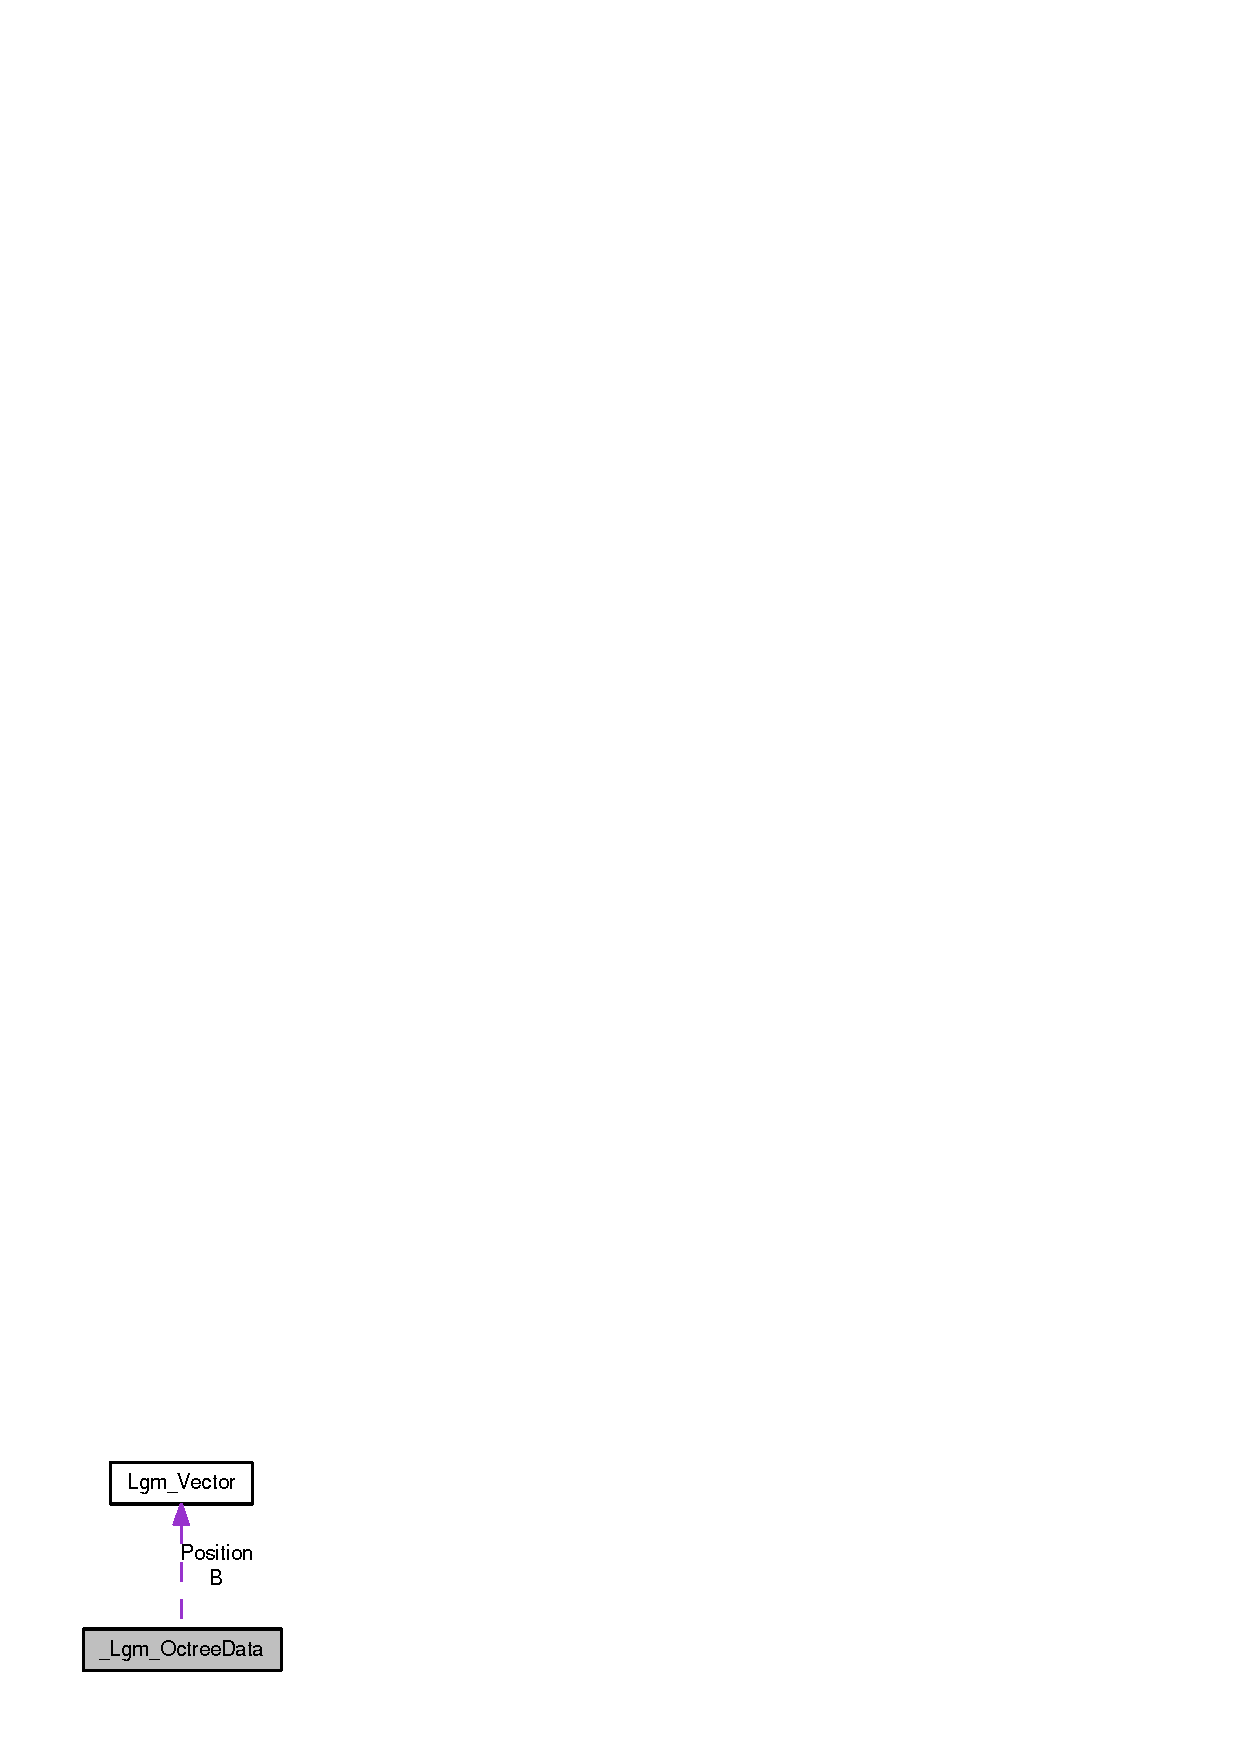
\includegraphics[width=138pt]{struct___lgm___octree_data__coll__graph}
\end{center}
\end{figure}
\subsection*{Data Fields}
\begin{CompactItemize}
\item 
\hyperlink{struct_lgm___vector}{Lgm\_\-Vector} \hyperlink{struct___lgm___octree_data_5dc98779b36676034ccefe5094251c55}{Position}
\item 
\hyperlink{struct_lgm___vector}{Lgm\_\-Vector} \hyperlink{struct___lgm___octree_data_867ec249dee38c139df965aa1611ed2a}{B}
\item 
double \hyperlink{struct___lgm___octree_data_527416adf36035c3ea5799827e7cd8b9}{Dist2}
\end{CompactItemize}


\subsection{Detailed Description}


Definition at line 22 of file Lgm\_\-Octree.h.

\subsection{Field Documentation}
\hypertarget{struct___lgm___octree_data_5dc98779b36676034ccefe5094251c55}{
\index{\_\-Lgm\_\-OctreeData@{\_\-Lgm\_\-OctreeData}!Position@{Position}}
\index{Position@{Position}!_Lgm_OctreeData@{\_\-Lgm\_\-OctreeData}}
\subsubsection[{Position}]{\setlength{\rightskip}{0pt plus 5cm}{\bf Lgm\_\-Vector} {\bf Position}}}
\label{struct___lgm___octree_data_5dc98779b36676034ccefe5094251c55}




Definition at line 24 of file Lgm\_\-Octree.h.\hypertarget{struct___lgm___octree_data_867ec249dee38c139df965aa1611ed2a}{
\index{\_\-Lgm\_\-OctreeData@{\_\-Lgm\_\-OctreeData}!B@{B}}
\index{B@{B}!_Lgm_OctreeData@{\_\-Lgm\_\-OctreeData}}
\subsubsection[{B}]{\setlength{\rightskip}{0pt plus 5cm}{\bf Lgm\_\-Vector} {\bf B}}}
\label{struct___lgm___octree_data_867ec249dee38c139df965aa1611ed2a}




Definition at line 25 of file Lgm\_\-Octree.h.\hypertarget{struct___lgm___octree_data_527416adf36035c3ea5799827e7cd8b9}{
\index{\_\-Lgm\_\-OctreeData@{\_\-Lgm\_\-OctreeData}!Dist2@{Dist2}}
\index{Dist2@{Dist2}!_Lgm_OctreeData@{\_\-Lgm\_\-OctreeData}}
\subsubsection[{Dist2}]{\setlength{\rightskip}{0pt plus 5cm}double {\bf Dist2}}}
\label{struct___lgm___octree_data_527416adf36035c3ea5799827e7cd8b9}




Definition at line 26 of file Lgm\_\-Octree.h.

The documentation for this struct was generated from the following file:\begin{CompactItemize}
\item 
/home/mgh/LanlGeoMag/libLanlGeoMag/Lgm/\hyperlink{_lgm___octree_8h}{Lgm\_\-Octree.h}\end{CompactItemize}

\hypertarget{struct__p_queue}{
\section{\_\-pQueue Struct Reference}
\label{struct__p_queue}\index{\_\-pQueue@{\_\-pQueue}}
}
{\tt \#include $<$Lgm\_\-Octree.h$>$}

Collaboration diagram for \_\-pQueue:\nopagebreak
\begin{figure}[H]
\begin{center}
\leavevmode
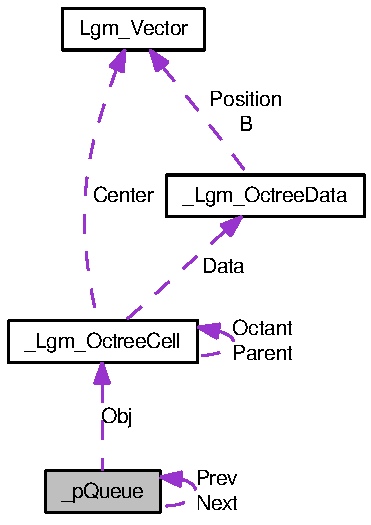
\includegraphics[width=214pt]{struct__p_queue__coll__graph}
\end{center}
\end{figure}
\subsection*{Data Fields}
\begin{CompactItemize}
\item 
\hyperlink{struct___lgm___octree_cell}{Lgm\_\-OctreeCell} $\ast$ \hyperlink{struct__p_queue_7530efafe5945a266bf8383ae47c7228}{Obj}
\item 
double \hyperlink{struct__p_queue_fcb495567b98cde535c5239b17681f62}{MinDist2}
\item 
int \hyperlink{struct__p_queue_270a4dbd002743db25f63825195e4006}{IsPoint}
\item 
int \hyperlink{struct__p_queue_37d972ae0b47b9099e30983131d31916}{j}
\item 
struct \hyperlink{struct__p_queue}{\_\-pQueue} $\ast$ \hyperlink{struct__p_queue_4717220aafe87eeda3986b3a258a2a2a}{Prev}
\item 
struct \hyperlink{struct__p_queue}{\_\-pQueue} $\ast$ \hyperlink{struct__p_queue_3a316f1387f6ede290905c4d79962b17}{Next}
\end{CompactItemize}


\subsection{Detailed Description}


Definition at line 59 of file Lgm\_\-Octree.h.

\subsection{Field Documentation}
\hypertarget{struct__p_queue_7530efafe5945a266bf8383ae47c7228}{
\index{\_\-pQueue@{\_\-pQueue}!Obj@{Obj}}
\index{Obj@{Obj}!_pQueue@{\_\-pQueue}}
\subsubsection[{Obj}]{\setlength{\rightskip}{0pt plus 5cm}{\bf Lgm\_\-OctreeCell}$\ast$ {\bf Obj}}}
\label{struct__p_queue_7530efafe5945a266bf8383ae47c7228}




Definition at line 61 of file Lgm\_\-Octree.h.\hypertarget{struct__p_queue_fcb495567b98cde535c5239b17681f62}{
\index{\_\-pQueue@{\_\-pQueue}!MinDist2@{MinDist2}}
\index{MinDist2@{MinDist2}!_pQueue@{\_\-pQueue}}
\subsubsection[{MinDist2}]{\setlength{\rightskip}{0pt plus 5cm}double {\bf MinDist2}}}
\label{struct__p_queue_fcb495567b98cde535c5239b17681f62}




Definition at line 62 of file Lgm\_\-Octree.h.\hypertarget{struct__p_queue_270a4dbd002743db25f63825195e4006}{
\index{\_\-pQueue@{\_\-pQueue}!IsPoint@{IsPoint}}
\index{IsPoint@{IsPoint}!_pQueue@{\_\-pQueue}}
\subsubsection[{IsPoint}]{\setlength{\rightskip}{0pt plus 5cm}int {\bf IsPoint}}}
\label{struct__p_queue_270a4dbd002743db25f63825195e4006}




Definition at line 65 of file Lgm\_\-Octree.h.\hypertarget{struct__p_queue_37d972ae0b47b9099e30983131d31916}{
\index{\_\-pQueue@{\_\-pQueue}!j@{j}}
\index{j@{j}!_pQueue@{\_\-pQueue}}
\subsubsection[{j}]{\setlength{\rightskip}{0pt plus 5cm}int {\bf j}}}
\label{struct__p_queue_37d972ae0b47b9099e30983131d31916}




Definition at line 67 of file Lgm\_\-Octree.h.\hypertarget{struct__p_queue_4717220aafe87eeda3986b3a258a2a2a}{
\index{\_\-pQueue@{\_\-pQueue}!Prev@{Prev}}
\index{Prev@{Prev}!_pQueue@{\_\-pQueue}}
\subsubsection[{Prev}]{\setlength{\rightskip}{0pt plus 5cm}struct {\bf \_\-pQueue}$\ast$ {\bf Prev}\hspace{0.3cm}{\tt  \mbox{[}read\mbox{]}}}}
\label{struct__p_queue_4717220aafe87eeda3986b3a258a2a2a}




Definition at line 69 of file Lgm\_\-Octree.h.\hypertarget{struct__p_queue_3a316f1387f6ede290905c4d79962b17}{
\index{\_\-pQueue@{\_\-pQueue}!Next@{Next}}
\index{Next@{Next}!_pQueue@{\_\-pQueue}}
\subsubsection[{Next}]{\setlength{\rightskip}{0pt plus 5cm}struct {\bf \_\-pQueue}$\ast$ {\bf Next}\hspace{0.3cm}{\tt  \mbox{[}read\mbox{]}}}}
\label{struct__p_queue_3a316f1387f6ede290905c4d79962b17}




Definition at line 70 of file Lgm\_\-Octree.h.

The documentation for this struct was generated from the following file:\begin{CompactItemize}
\item 
/home/mgh/LanlGeoMag/libLanlGeoMag/Lgm/\hyperlink{_lgm___octree_8h}{Lgm\_\-Octree.h}\end{CompactItemize}

\hypertarget{struct___sgp_info}{
\section{\_\-SgpInfo Struct Reference}
\label{struct___sgp_info}\index{\_\-SgpInfo@{\_\-SgpInfo}}
}
{\tt \#include $<$Lgm\_\-Sgp.h$>$}

\subsection*{Data Fields}
\begin{CompactItemize}
\item 
int \hyperlink{struct___sgp_info_686aa728d7bead181dc3ac3a0832502f}{IFLAG}
\item 
double \hyperlink{struct___sgp_info_b8bbf06d285fc56edffbc353b8e1acf6}{XMO}
\item 
double \hyperlink{struct___sgp_info_19011c821f658fe3d9eb170b9a7d505d}{XNODEO}
\item 
double \hyperlink{struct___sgp_info_06f0e6ec3e46d144a3fc90417308816e}{OMEGAO}
\item 
double \hyperlink{struct___sgp_info_c3b3a39803395c18d0919adaef671344}{EO}
\item 
double \hyperlink{struct___sgp_info_f3ee830bb3dfcd5873b48ac804fcfcfc}{XINCL}
\item 
double \hyperlink{struct___sgp_info_3a911c89d654142a00f0502b3ff5ccae}{XNO}
\item 
double \hyperlink{struct___sgp_info_524a63b4890023f57824dbd323fa4bc8}{XNDT2O}
\item 
double \hyperlink{struct___sgp_info_317e80d6b4bbe1395b92c56947740716}{XNDD6O}
\item 
double \hyperlink{struct___sgp_info_44e631843bf304236d4a37d7ce0ef549}{BSTAR}
\item 
double \hyperlink{struct___sgp_info_3c2788a0eb0527cf6b39bf2efcedc9d8}{XDOT}
\item 
double \hyperlink{struct___sgp_info_63b51d09dc1b7c17d7822ecf0276c303}{YDOT}
\item 
double \hyperlink{struct___sgp_info_0113995221a55c2a324a49b992c3e83e}{ZDOT}
\item 
double \hyperlink{struct___sgp_info_096845c6ff00da184a48b51ea1efde49}{EPOCH}
\item 
double \hyperlink{struct___sgp_info_105c57f6cb86a5a9c93a1454db061841}{DS50}
\item 
double \hyperlink{struct___sgp_info_c9dd4d43db3b68465f53fd7841f2cb96}{argpdot}
\item 
double \hyperlink{struct___sgp_info_48e2d1161d18da867e275aad47a0f2f5}{argpo}
\item 
double \hyperlink{struct___sgp_info_ec7bcb1d46812f966d89f66dc1a399ea}{atime}
\item 
double \hyperlink{struct___sgp_info_73cf6efaf6896931cb677e94a7d95b4a}{aycof}
\item 
double \hyperlink{struct___sgp_info_e385ed1815b61e4a30b2ab3165514f71}{bstar}
\item 
double \hyperlink{struct___sgp_info_d32764e5a4a660af7424fb205e2eca4c}{cc1}
\item 
double \hyperlink{struct___sgp_info_aefb3346680163a2f54c8115c6542e94}{cc4}
\item 
double \hyperlink{struct___sgp_info_02926a7d267c9362ca676c008f4e6c21}{cc5}
\item 
double \hyperlink{struct___sgp_info_77fbcbf60585b0d443d82036a943d947}{con41}
\item 
double \hyperlink{struct___sgp_info_13b4e96542fec65c7a11bc18f5a5439e}{d2}
\item 
double \hyperlink{struct___sgp_info_230a89ad405323f2b9926a19395ec04e}{d2201}
\item 
double \hyperlink{struct___sgp_info_548a2513409777664a0675a48be0c85a}{d2211}
\item 
double \hyperlink{struct___sgp_info_483620916658141a26a261c7a5016910}{d3}
\item 
double \hyperlink{struct___sgp_info_a7e79e7ab67d28da1b1b3dac80810655}{d3210}
\item 
double \hyperlink{struct___sgp_info_01655415f454f2f669b0055791fdd7fb}{d3222}
\item 
double \hyperlink{struct___sgp_info_4bdca1913dad0bca307e04c2c8128100}{d4}
\item 
double \hyperlink{struct___sgp_info_0b8afbe4b3eaca5ad5d895e7e6bb0da3}{d4410}
\item 
double \hyperlink{struct___sgp_info_71ff139b8068f058073bd65be4a038a4}{d4422}
\item 
double \hyperlink{struct___sgp_info_bdd287076f628dd8963e31918c477f27}{d5220}
\item 
double \hyperlink{struct___sgp_info_6029959a3ce7b1deec5862dab9dc928b}{d5232}
\item 
double \hyperlink{struct___sgp_info_27382a4e06e4d963a2e268a4e47eb639}{d5421}
\item 
double \hyperlink{struct___sgp_info_ed583d24183bddfa0eb67ca6653c9a42}{d5433}
\item 
double \hyperlink{struct___sgp_info_6c4a3f7535bef01f2fb7aa8ae65a1a63}{dedt}
\item 
double \hyperlink{struct___sgp_info_8c5ee7600289061b966b0e64ba835e66}{del1}
\item 
double \hyperlink{struct___sgp_info_f52c4e502051877edca1aec48acabd34}{del2}
\item 
double \hyperlink{struct___sgp_info_d460879243bdba4b857df0fe993443fe}{del3}
\item 
double \hyperlink{struct___sgp_info_a4f8567c544bb137f5dc25957c63ac1a}{delmo}
\item 
double \hyperlink{struct___sgp_info_b4f69178e71cb056b53415896f5de48e}{didt}
\item 
double \hyperlink{struct___sgp_info_97de9b0087d69e56ed6d89a5d6caef17}{dmdt}
\item 
double \hyperlink{struct___sgp_info_eb1fbdf7c8b859e1d4d0212ccc5c903c}{dnodt}
\item 
double \hyperlink{struct___sgp_info_17500bc363ef2d910381b0b5999c4aaa}{domdt}
\item 
double \hyperlink{struct___sgp_info_ff99da95c225d58a2c9acf9aa04a267b}{e3}
\item 
double \hyperlink{struct___sgp_info_9c6fbcc6053a01f83f538705162576d1}{ecco}
\item 
double \hyperlink{struct___sgp_info_3907e33c8e58cb154a33174dd8e78179}{ee2}
\item 
double \hyperlink{struct___sgp_info_1ec236df65b93a338aecdf3fa64790f9}{error}
\item 
double \hyperlink{struct___sgp_info_e4f402913d5fc5dd3aebca242ab26019}{eta}
\item 
double \hyperlink{struct___sgp_info_a25f72b7facd9726153a3161507fd71e}{gsto}
\item 
double \hyperlink{struct___sgp_info_fcbd011ce32e4763767d90522dc42e0e}{inclo}
\item 
double \hyperlink{struct___sgp_info_ee90111c98406414a1db98e8c5102e4f}{mdot}
\item 
double \hyperlink{struct___sgp_info_bf05d62d7ad39d494816d23dd19b9325}{mo}
\item 
double \hyperlink{struct___sgp_info_b002ef35361da13209d5bf20414b08b1}{no}
\item 
double \hyperlink{struct___sgp_info_6ec196aa951f2b53cdbfd43947eb2bce}{nodecf}
\item 
double \hyperlink{struct___sgp_info_9a7d9ae35fbeac8903eb8ebf5f9d31cc}{nodedot}
\item 
double \hyperlink{struct___sgp_info_8496b25cf07aff8b5d0944cc2e229778}{nodeo}
\item 
double \hyperlink{struct___sgp_info_9b0060ff74bc3469f158f9d4cfa578ea}{omgcof}
\item 
double \hyperlink{struct___sgp_info_689de6e0b3caffccb68dcee94abb1018}{peo}
\item 
double \hyperlink{struct___sgp_info_f56cf39324cbf2fe295bf84dc69e3e8f}{pgho}
\item 
double \hyperlink{struct___sgp_info_6455bb211516d721115c708d51f5beec}{pho}
\item 
double \hyperlink{struct___sgp_info_3063db50044a10a1805f09ec06904db9}{pinco}
\item 
double \hyperlink{struct___sgp_info_7ad4147f4ca4a74315a064ca7b1817f5}{plo}
\item 
double \hyperlink{struct___sgp_info_5a7f7150e4e1afe1ca272a66d2618936}{se2}
\item 
double \hyperlink{struct___sgp_info_7881e839568571e07c209edcdf9ac468}{se3}
\item 
double \hyperlink{struct___sgp_info_77544b4b59fd16ed1ac93adfee0eb997}{sgh2}
\item 
double \hyperlink{struct___sgp_info_d42d32067016e78f4583075ea03773b2}{sgh3}
\item 
double \hyperlink{struct___sgp_info_8333fff103deda5ec256d39b38beabf3}{sgh4}
\item 
double \hyperlink{struct___sgp_info_f39a6d6ec64bcb919784f1c046a5031d}{sh2}
\item 
double \hyperlink{struct___sgp_info_9081e5546a5c993436dcc994592f0c7a}{sh3}
\item 
double \hyperlink{struct___sgp_info_61a1945bc1d3f4c395b657c4203ceb2a}{si2}
\item 
double \hyperlink{struct___sgp_info_5e144ba52a7d297f9c6dfcd5380e49d1}{si3}
\item 
double \hyperlink{struct___sgp_info_ac6611ed753f0b5e0e50d51f6a8fc3b8}{sinmao}
\item 
double \hyperlink{struct___sgp_info_24aba20cbbf42da0d081954b34834924}{sl2}
\item 
double \hyperlink{struct___sgp_info_18b9a2f918f88752c91b220bf3531d31}{sl3}
\item 
double \hyperlink{struct___sgp_info_234f391445ad2c9894442de5280d0559}{sl4}
\item 
double \hyperlink{struct___sgp_info_87accd1af8e0aff4b818d891374f7cec}{t}
\item 
double \hyperlink{struct___sgp_info_a92271ca6d86502933389f47a9202ab6}{t2cof}
\item 
double \hyperlink{struct___sgp_info_6ead2ed42d4de4759c2a773cbc10d36c}{t3cof}
\item 
double \hyperlink{struct___sgp_info_9fba2bddd10102492866a46693318781}{t4cof}
\item 
double \hyperlink{struct___sgp_info_3770068f50d6a8b4a73dcec1e8967087}{t5cof}
\item 
double \hyperlink{struct___sgp_info_1e0131f4c92de0fd372d35e3b9edb9f4}{x1mth2}
\item 
double \hyperlink{struct___sgp_info_1db2d8883d9dd784b6ae51a031c1266e}{x7thm1}
\item 
double \hyperlink{struct___sgp_info_34389a85dd8a65ed941cc23793d4efbf}{xfact}
\item 
double \hyperlink{struct___sgp_info_12cc589dda276aa5ae735902e6778b7c}{xgh2}
\item 
double \hyperlink{struct___sgp_info_e49feebf68831d39731fa268baba51c1}{xgh3}
\item 
double \hyperlink{struct___sgp_info_c1fc37ddfcd1eb053bb240d30083455d}{xgh4}
\item 
double \hyperlink{struct___sgp_info_1ae6115c362e5b5450b515b208f46764}{xh2}
\item 
double \hyperlink{struct___sgp_info_b8a252c46a5859f5f5f5f7a3bb0ed3b8}{xh3}
\item 
double \hyperlink{struct___sgp_info_c3b4de799b764c0819cffc7166a2df10}{xi2}
\item 
double \hyperlink{struct___sgp_info_90e3204b70e2fc9053c1879656ca4bc7}{xi3}
\item 
double \hyperlink{struct___sgp_info_965576393853e94605542dbd4df08cfe}{xl2}
\item 
double \hyperlink{struct___sgp_info_db2bab7e771a89101eaf1dd3d527fcf3}{xl3}
\item 
double \hyperlink{struct___sgp_info_5233fa6736de1f47b91f58865ea7cb80}{xl4}
\item 
double \hyperlink{struct___sgp_info_53f269b680646e524c0d190ceea30d2d}{xlamo}
\item 
double \hyperlink{struct___sgp_info_0af92c37e7066a1cb310fb71c91ad369}{xlcof}
\item 
double \hyperlink{struct___sgp_info_83e99efa0cbc63cd4bad3b0bff321c80}{xli}
\item 
double \hyperlink{struct___sgp_info_f47d9394629b013547ccd3a29072de44}{xmcof}
\item 
double \hyperlink{struct___sgp_info_cfea2ed90198863a579d0dd9123d2e7b}{xni}
\item 
double \hyperlink{struct___sgp_info_0c8d59633bdce5d61494b16c884903bd}{zmol}
\item 
double \hyperlink{struct___sgp_info_1840b955ac5e5eb7d015f46051df589f}{zmos}
\item 
int \hyperlink{struct___sgp_info_a69491b0e6ccf4560cce706b1e089e24}{GravConst}
\item 
int \hyperlink{struct___sgp_info_2d01b296d1d4611e60cda302675ef46e}{irez}
\item 
char \hyperlink{struct___sgp_info_6a9691d2260a0c4c1a531b79d708520a}{init}
\item 
char \hyperlink{struct___sgp_info_e16a2e07e3ca49c3c4bd592efbf1b5ed}{method}
\item 
char \hyperlink{struct___sgp_info_633c6d59b92dbf5b830ea47a87b9fc96}{isimp}
\item 
double \hyperlink{struct___sgp_info_1059b82f84827fc49ea81b12566b3cdb}{X}
\item 
double \hyperlink{struct___sgp_info_c8d59bf77d5ef21e7c7a88b08f14c825}{Y}
\item 
double \hyperlink{struct___sgp_info_0f16a8f561453187897f0820186da39b}{Z}
\item 
double \hyperlink{struct___sgp_info_7a2579ee60469b7dc5ac77b902d71fa5}{VX}
\item 
double \hyperlink{struct___sgp_info_f7687d7aef9103def7b09bcb5d568e04}{VY}
\item 
double \hyperlink{struct___sgp_info_b9b9161b8168f9424231c7fc59837f88}{VZ}
\end{CompactItemize}


\subsection{Detailed Description}


Definition at line 105 of file Lgm\_\-Sgp.h.

\subsection{Field Documentation}
\hypertarget{struct___sgp_info_686aa728d7bead181dc3ac3a0832502f}{
\index{\_\-SgpInfo@{\_\-SgpInfo}!IFLAG@{IFLAG}}
\index{IFLAG@{IFLAG}!_SgpInfo@{\_\-SgpInfo}}
\subsubsection[{IFLAG}]{\setlength{\rightskip}{0pt plus 5cm}int {\bf IFLAG}}}
\label{struct___sgp_info_686aa728d7bead181dc3ac3a0832502f}




Definition at line 110 of file Lgm\_\-Sgp.h.\hypertarget{struct___sgp_info_b8bbf06d285fc56edffbc353b8e1acf6}{
\index{\_\-SgpInfo@{\_\-SgpInfo}!XMO@{XMO}}
\index{XMO@{XMO}!_SgpInfo@{\_\-SgpInfo}}
\subsubsection[{XMO}]{\setlength{\rightskip}{0pt plus 5cm}double {\bf XMO}}}
\label{struct___sgp_info_b8bbf06d285fc56edffbc353b8e1acf6}




Definition at line 111 of file Lgm\_\-Sgp.h.\hypertarget{struct___sgp_info_19011c821f658fe3d9eb170b9a7d505d}{
\index{\_\-SgpInfo@{\_\-SgpInfo}!XNODEO@{XNODEO}}
\index{XNODEO@{XNODEO}!_SgpInfo@{\_\-SgpInfo}}
\subsubsection[{XNODEO}]{\setlength{\rightskip}{0pt plus 5cm}double {\bf XNODEO}}}
\label{struct___sgp_info_19011c821f658fe3d9eb170b9a7d505d}




Definition at line 112 of file Lgm\_\-Sgp.h.\hypertarget{struct___sgp_info_06f0e6ec3e46d144a3fc90417308816e}{
\index{\_\-SgpInfo@{\_\-SgpInfo}!OMEGAO@{OMEGAO}}
\index{OMEGAO@{OMEGAO}!_SgpInfo@{\_\-SgpInfo}}
\subsubsection[{OMEGAO}]{\setlength{\rightskip}{0pt plus 5cm}double {\bf OMEGAO}}}
\label{struct___sgp_info_06f0e6ec3e46d144a3fc90417308816e}




Definition at line 113 of file Lgm\_\-Sgp.h.\hypertarget{struct___sgp_info_c3b3a39803395c18d0919adaef671344}{
\index{\_\-SgpInfo@{\_\-SgpInfo}!EO@{EO}}
\index{EO@{EO}!_SgpInfo@{\_\-SgpInfo}}
\subsubsection[{EO}]{\setlength{\rightskip}{0pt plus 5cm}double {\bf EO}}}
\label{struct___sgp_info_c3b3a39803395c18d0919adaef671344}




Definition at line 114 of file Lgm\_\-Sgp.h.\hypertarget{struct___sgp_info_f3ee830bb3dfcd5873b48ac804fcfcfc}{
\index{\_\-SgpInfo@{\_\-SgpInfo}!XINCL@{XINCL}}
\index{XINCL@{XINCL}!_SgpInfo@{\_\-SgpInfo}}
\subsubsection[{XINCL}]{\setlength{\rightskip}{0pt plus 5cm}double {\bf XINCL}}}
\label{struct___sgp_info_f3ee830bb3dfcd5873b48ac804fcfcfc}




Definition at line 115 of file Lgm\_\-Sgp.h.\hypertarget{struct___sgp_info_3a911c89d654142a00f0502b3ff5ccae}{
\index{\_\-SgpInfo@{\_\-SgpInfo}!XNO@{XNO}}
\index{XNO@{XNO}!_SgpInfo@{\_\-SgpInfo}}
\subsubsection[{XNO}]{\setlength{\rightskip}{0pt plus 5cm}double {\bf XNO}}}
\label{struct___sgp_info_3a911c89d654142a00f0502b3ff5ccae}




Definition at line 116 of file Lgm\_\-Sgp.h.\hypertarget{struct___sgp_info_524a63b4890023f57824dbd323fa4bc8}{
\index{\_\-SgpInfo@{\_\-SgpInfo}!XNDT2O@{XNDT2O}}
\index{XNDT2O@{XNDT2O}!_SgpInfo@{\_\-SgpInfo}}
\subsubsection[{XNDT2O}]{\setlength{\rightskip}{0pt plus 5cm}double {\bf XNDT2O}}}
\label{struct___sgp_info_524a63b4890023f57824dbd323fa4bc8}




Definition at line 117 of file Lgm\_\-Sgp.h.\hypertarget{struct___sgp_info_317e80d6b4bbe1395b92c56947740716}{
\index{\_\-SgpInfo@{\_\-SgpInfo}!XNDD6O@{XNDD6O}}
\index{XNDD6O@{XNDD6O}!_SgpInfo@{\_\-SgpInfo}}
\subsubsection[{XNDD6O}]{\setlength{\rightskip}{0pt plus 5cm}double {\bf XNDD6O}}}
\label{struct___sgp_info_317e80d6b4bbe1395b92c56947740716}




Definition at line 118 of file Lgm\_\-Sgp.h.\hypertarget{struct___sgp_info_44e631843bf304236d4a37d7ce0ef549}{
\index{\_\-SgpInfo@{\_\-SgpInfo}!BSTAR@{BSTAR}}
\index{BSTAR@{BSTAR}!_SgpInfo@{\_\-SgpInfo}}
\subsubsection[{BSTAR}]{\setlength{\rightskip}{0pt plus 5cm}double {\bf BSTAR}}}
\label{struct___sgp_info_44e631843bf304236d4a37d7ce0ef549}




Definition at line 119 of file Lgm\_\-Sgp.h.\hypertarget{struct___sgp_info_3c2788a0eb0527cf6b39bf2efcedc9d8}{
\index{\_\-SgpInfo@{\_\-SgpInfo}!XDOT@{XDOT}}
\index{XDOT@{XDOT}!_SgpInfo@{\_\-SgpInfo}}
\subsubsection[{XDOT}]{\setlength{\rightskip}{0pt plus 5cm}double {\bf XDOT}}}
\label{struct___sgp_info_3c2788a0eb0527cf6b39bf2efcedc9d8}




Definition at line 123 of file Lgm\_\-Sgp.h.\hypertarget{struct___sgp_info_63b51d09dc1b7c17d7822ecf0276c303}{
\index{\_\-SgpInfo@{\_\-SgpInfo}!YDOT@{YDOT}}
\index{YDOT@{YDOT}!_SgpInfo@{\_\-SgpInfo}}
\subsubsection[{YDOT}]{\setlength{\rightskip}{0pt plus 5cm}double {\bf YDOT}}}
\label{struct___sgp_info_63b51d09dc1b7c17d7822ecf0276c303}




Definition at line 124 of file Lgm\_\-Sgp.h.\hypertarget{struct___sgp_info_0113995221a55c2a324a49b992c3e83e}{
\index{\_\-SgpInfo@{\_\-SgpInfo}!ZDOT@{ZDOT}}
\index{ZDOT@{ZDOT}!_SgpInfo@{\_\-SgpInfo}}
\subsubsection[{ZDOT}]{\setlength{\rightskip}{0pt plus 5cm}double {\bf ZDOT}}}
\label{struct___sgp_info_0113995221a55c2a324a49b992c3e83e}




Definition at line 125 of file Lgm\_\-Sgp.h.\hypertarget{struct___sgp_info_096845c6ff00da184a48b51ea1efde49}{
\index{\_\-SgpInfo@{\_\-SgpInfo}!EPOCH@{EPOCH}}
\index{EPOCH@{EPOCH}!_SgpInfo@{\_\-SgpInfo}}
\subsubsection[{EPOCH}]{\setlength{\rightskip}{0pt plus 5cm}double {\bf EPOCH}}}
\label{struct___sgp_info_096845c6ff00da184a48b51ea1efde49}




Definition at line 126 of file Lgm\_\-Sgp.h.\hypertarget{struct___sgp_info_105c57f6cb86a5a9c93a1454db061841}{
\index{\_\-SgpInfo@{\_\-SgpInfo}!DS50@{DS50}}
\index{DS50@{DS50}!_SgpInfo@{\_\-SgpInfo}}
\subsubsection[{DS50}]{\setlength{\rightskip}{0pt plus 5cm}double {\bf DS50}}}
\label{struct___sgp_info_105c57f6cb86a5a9c93a1454db061841}




Definition at line 127 of file Lgm\_\-Sgp.h.\hypertarget{struct___sgp_info_c9dd4d43db3b68465f53fd7841f2cb96}{
\index{\_\-SgpInfo@{\_\-SgpInfo}!argpdot@{argpdot}}
\index{argpdot@{argpdot}!_SgpInfo@{\_\-SgpInfo}}
\subsubsection[{argpdot}]{\setlength{\rightskip}{0pt plus 5cm}double {\bf argpdot}}}
\label{struct___sgp_info_c9dd4d43db3b68465f53fd7841f2cb96}




Definition at line 132 of file Lgm\_\-Sgp.h.\hypertarget{struct___sgp_info_48e2d1161d18da867e275aad47a0f2f5}{
\index{\_\-SgpInfo@{\_\-SgpInfo}!argpo@{argpo}}
\index{argpo@{argpo}!_SgpInfo@{\_\-SgpInfo}}
\subsubsection[{argpo}]{\setlength{\rightskip}{0pt plus 5cm}double {\bf argpo}}}
\label{struct___sgp_info_48e2d1161d18da867e275aad47a0f2f5}




Definition at line 132 of file Lgm\_\-Sgp.h.\hypertarget{struct___sgp_info_ec7bcb1d46812f966d89f66dc1a399ea}{
\index{\_\-SgpInfo@{\_\-SgpInfo}!atime@{atime}}
\index{atime@{atime}!_SgpInfo@{\_\-SgpInfo}}
\subsubsection[{atime}]{\setlength{\rightskip}{0pt plus 5cm}double {\bf atime}}}
\label{struct___sgp_info_ec7bcb1d46812f966d89f66dc1a399ea}




Definition at line 132 of file Lgm\_\-Sgp.h.\hypertarget{struct___sgp_info_73cf6efaf6896931cb677e94a7d95b4a}{
\index{\_\-SgpInfo@{\_\-SgpInfo}!aycof@{aycof}}
\index{aycof@{aycof}!_SgpInfo@{\_\-SgpInfo}}
\subsubsection[{aycof}]{\setlength{\rightskip}{0pt plus 5cm}double {\bf aycof}}}
\label{struct___sgp_info_73cf6efaf6896931cb677e94a7d95b4a}




Definition at line 132 of file Lgm\_\-Sgp.h.\hypertarget{struct___sgp_info_e385ed1815b61e4a30b2ab3165514f71}{
\index{\_\-SgpInfo@{\_\-SgpInfo}!bstar@{bstar}}
\index{bstar@{bstar}!_SgpInfo@{\_\-SgpInfo}}
\subsubsection[{bstar}]{\setlength{\rightskip}{0pt plus 5cm}double {\bf bstar}}}
\label{struct___sgp_info_e385ed1815b61e4a30b2ab3165514f71}




Definition at line 132 of file Lgm\_\-Sgp.h.\hypertarget{struct___sgp_info_d32764e5a4a660af7424fb205e2eca4c}{
\index{\_\-SgpInfo@{\_\-SgpInfo}!cc1@{cc1}}
\index{cc1@{cc1}!_SgpInfo@{\_\-SgpInfo}}
\subsubsection[{cc1}]{\setlength{\rightskip}{0pt plus 5cm}double {\bf cc1}}}
\label{struct___sgp_info_d32764e5a4a660af7424fb205e2eca4c}




Definition at line 132 of file Lgm\_\-Sgp.h.\hypertarget{struct___sgp_info_aefb3346680163a2f54c8115c6542e94}{
\index{\_\-SgpInfo@{\_\-SgpInfo}!cc4@{cc4}}
\index{cc4@{cc4}!_SgpInfo@{\_\-SgpInfo}}
\subsubsection[{cc4}]{\setlength{\rightskip}{0pt plus 5cm}double {\bf cc4}}}
\label{struct___sgp_info_aefb3346680163a2f54c8115c6542e94}




Definition at line 132 of file Lgm\_\-Sgp.h.\hypertarget{struct___sgp_info_02926a7d267c9362ca676c008f4e6c21}{
\index{\_\-SgpInfo@{\_\-SgpInfo}!cc5@{cc5}}
\index{cc5@{cc5}!_SgpInfo@{\_\-SgpInfo}}
\subsubsection[{cc5}]{\setlength{\rightskip}{0pt plus 5cm}double {\bf cc5}}}
\label{struct___sgp_info_02926a7d267c9362ca676c008f4e6c21}




Definition at line 132 of file Lgm\_\-Sgp.h.\hypertarget{struct___sgp_info_77fbcbf60585b0d443d82036a943d947}{
\index{\_\-SgpInfo@{\_\-SgpInfo}!con41@{con41}}
\index{con41@{con41}!_SgpInfo@{\_\-SgpInfo}}
\subsubsection[{con41}]{\setlength{\rightskip}{0pt plus 5cm}double {\bf con41}}}
\label{struct___sgp_info_77fbcbf60585b0d443d82036a943d947}




Definition at line 132 of file Lgm\_\-Sgp.h.\hypertarget{struct___sgp_info_13b4e96542fec65c7a11bc18f5a5439e}{
\index{\_\-SgpInfo@{\_\-SgpInfo}!d2@{d2}}
\index{d2@{d2}!_SgpInfo@{\_\-SgpInfo}}
\subsubsection[{d2}]{\setlength{\rightskip}{0pt plus 5cm}double {\bf d2}}}
\label{struct___sgp_info_13b4e96542fec65c7a11bc18f5a5439e}




Definition at line 132 of file Lgm\_\-Sgp.h.\hypertarget{struct___sgp_info_230a89ad405323f2b9926a19395ec04e}{
\index{\_\-SgpInfo@{\_\-SgpInfo}!d2201@{d2201}}
\index{d2201@{d2201}!_SgpInfo@{\_\-SgpInfo}}
\subsubsection[{d2201}]{\setlength{\rightskip}{0pt plus 5cm}double {\bf d2201}}}
\label{struct___sgp_info_230a89ad405323f2b9926a19395ec04e}




Definition at line 132 of file Lgm\_\-Sgp.h.\hypertarget{struct___sgp_info_548a2513409777664a0675a48be0c85a}{
\index{\_\-SgpInfo@{\_\-SgpInfo}!d2211@{d2211}}
\index{d2211@{d2211}!_SgpInfo@{\_\-SgpInfo}}
\subsubsection[{d2211}]{\setlength{\rightskip}{0pt plus 5cm}double {\bf d2211}}}
\label{struct___sgp_info_548a2513409777664a0675a48be0c85a}




Definition at line 132 of file Lgm\_\-Sgp.h.\hypertarget{struct___sgp_info_483620916658141a26a261c7a5016910}{
\index{\_\-SgpInfo@{\_\-SgpInfo}!d3@{d3}}
\index{d3@{d3}!_SgpInfo@{\_\-SgpInfo}}
\subsubsection[{d3}]{\setlength{\rightskip}{0pt plus 5cm}double {\bf d3}}}
\label{struct___sgp_info_483620916658141a26a261c7a5016910}




Definition at line 133 of file Lgm\_\-Sgp.h.\hypertarget{struct___sgp_info_a7e79e7ab67d28da1b1b3dac80810655}{
\index{\_\-SgpInfo@{\_\-SgpInfo}!d3210@{d3210}}
\index{d3210@{d3210}!_SgpInfo@{\_\-SgpInfo}}
\subsubsection[{d3210}]{\setlength{\rightskip}{0pt plus 5cm}double {\bf d3210}}}
\label{struct___sgp_info_a7e79e7ab67d28da1b1b3dac80810655}




Definition at line 133 of file Lgm\_\-Sgp.h.\hypertarget{struct___sgp_info_01655415f454f2f669b0055791fdd7fb}{
\index{\_\-SgpInfo@{\_\-SgpInfo}!d3222@{d3222}}
\index{d3222@{d3222}!_SgpInfo@{\_\-SgpInfo}}
\subsubsection[{d3222}]{\setlength{\rightskip}{0pt plus 5cm}double {\bf d3222}}}
\label{struct___sgp_info_01655415f454f2f669b0055791fdd7fb}




Definition at line 133 of file Lgm\_\-Sgp.h.\hypertarget{struct___sgp_info_4bdca1913dad0bca307e04c2c8128100}{
\index{\_\-SgpInfo@{\_\-SgpInfo}!d4@{d4}}
\index{d4@{d4}!_SgpInfo@{\_\-SgpInfo}}
\subsubsection[{d4}]{\setlength{\rightskip}{0pt plus 5cm}double {\bf d4}}}
\label{struct___sgp_info_4bdca1913dad0bca307e04c2c8128100}




Definition at line 133 of file Lgm\_\-Sgp.h.\hypertarget{struct___sgp_info_0b8afbe4b3eaca5ad5d895e7e6bb0da3}{
\index{\_\-SgpInfo@{\_\-SgpInfo}!d4410@{d4410}}
\index{d4410@{d4410}!_SgpInfo@{\_\-SgpInfo}}
\subsubsection[{d4410}]{\setlength{\rightskip}{0pt plus 5cm}double {\bf d4410}}}
\label{struct___sgp_info_0b8afbe4b3eaca5ad5d895e7e6bb0da3}




Definition at line 133 of file Lgm\_\-Sgp.h.\hypertarget{struct___sgp_info_71ff139b8068f058073bd65be4a038a4}{
\index{\_\-SgpInfo@{\_\-SgpInfo}!d4422@{d4422}}
\index{d4422@{d4422}!_SgpInfo@{\_\-SgpInfo}}
\subsubsection[{d4422}]{\setlength{\rightskip}{0pt plus 5cm}double {\bf d4422}}}
\label{struct___sgp_info_71ff139b8068f058073bd65be4a038a4}




Definition at line 133 of file Lgm\_\-Sgp.h.\hypertarget{struct___sgp_info_bdd287076f628dd8963e31918c477f27}{
\index{\_\-SgpInfo@{\_\-SgpInfo}!d5220@{d5220}}
\index{d5220@{d5220}!_SgpInfo@{\_\-SgpInfo}}
\subsubsection[{d5220}]{\setlength{\rightskip}{0pt plus 5cm}double {\bf d5220}}}
\label{struct___sgp_info_bdd287076f628dd8963e31918c477f27}




Definition at line 133 of file Lgm\_\-Sgp.h.\hypertarget{struct___sgp_info_6029959a3ce7b1deec5862dab9dc928b}{
\index{\_\-SgpInfo@{\_\-SgpInfo}!d5232@{d5232}}
\index{d5232@{d5232}!_SgpInfo@{\_\-SgpInfo}}
\subsubsection[{d5232}]{\setlength{\rightskip}{0pt plus 5cm}double {\bf d5232}}}
\label{struct___sgp_info_6029959a3ce7b1deec5862dab9dc928b}




Definition at line 133 of file Lgm\_\-Sgp.h.\hypertarget{struct___sgp_info_27382a4e06e4d963a2e268a4e47eb639}{
\index{\_\-SgpInfo@{\_\-SgpInfo}!d5421@{d5421}}
\index{d5421@{d5421}!_SgpInfo@{\_\-SgpInfo}}
\subsubsection[{d5421}]{\setlength{\rightskip}{0pt plus 5cm}double {\bf d5421}}}
\label{struct___sgp_info_27382a4e06e4d963a2e268a4e47eb639}




Definition at line 133 of file Lgm\_\-Sgp.h.\hypertarget{struct___sgp_info_ed583d24183bddfa0eb67ca6653c9a42}{
\index{\_\-SgpInfo@{\_\-SgpInfo}!d5433@{d5433}}
\index{d5433@{d5433}!_SgpInfo@{\_\-SgpInfo}}
\subsubsection[{d5433}]{\setlength{\rightskip}{0pt plus 5cm}double {\bf d5433}}}
\label{struct___sgp_info_ed583d24183bddfa0eb67ca6653c9a42}




Definition at line 133 of file Lgm\_\-Sgp.h.\hypertarget{struct___sgp_info_6c4a3f7535bef01f2fb7aa8ae65a1a63}{
\index{\_\-SgpInfo@{\_\-SgpInfo}!dedt@{dedt}}
\index{dedt@{dedt}!_SgpInfo@{\_\-SgpInfo}}
\subsubsection[{dedt}]{\setlength{\rightskip}{0pt plus 5cm}double {\bf dedt}}}
\label{struct___sgp_info_6c4a3f7535bef01f2fb7aa8ae65a1a63}




Definition at line 133 of file Lgm\_\-Sgp.h.\hypertarget{struct___sgp_info_8c5ee7600289061b966b0e64ba835e66}{
\index{\_\-SgpInfo@{\_\-SgpInfo}!del1@{del1}}
\index{del1@{del1}!_SgpInfo@{\_\-SgpInfo}}
\subsubsection[{del1}]{\setlength{\rightskip}{0pt plus 5cm}double {\bf del1}}}
\label{struct___sgp_info_8c5ee7600289061b966b0e64ba835e66}




Definition at line 133 of file Lgm\_\-Sgp.h.\hypertarget{struct___sgp_info_f52c4e502051877edca1aec48acabd34}{
\index{\_\-SgpInfo@{\_\-SgpInfo}!del2@{del2}}
\index{del2@{del2}!_SgpInfo@{\_\-SgpInfo}}
\subsubsection[{del2}]{\setlength{\rightskip}{0pt plus 5cm}double {\bf del2}}}
\label{struct___sgp_info_f52c4e502051877edca1aec48acabd34}




Definition at line 134 of file Lgm\_\-Sgp.h.\hypertarget{struct___sgp_info_d460879243bdba4b857df0fe993443fe}{
\index{\_\-SgpInfo@{\_\-SgpInfo}!del3@{del3}}
\index{del3@{del3}!_SgpInfo@{\_\-SgpInfo}}
\subsubsection[{del3}]{\setlength{\rightskip}{0pt plus 5cm}double {\bf del3}}}
\label{struct___sgp_info_d460879243bdba4b857df0fe993443fe}




Definition at line 134 of file Lgm\_\-Sgp.h.\hypertarget{struct___sgp_info_a4f8567c544bb137f5dc25957c63ac1a}{
\index{\_\-SgpInfo@{\_\-SgpInfo}!delmo@{delmo}}
\index{delmo@{delmo}!_SgpInfo@{\_\-SgpInfo}}
\subsubsection[{delmo}]{\setlength{\rightskip}{0pt plus 5cm}double {\bf delmo}}}
\label{struct___sgp_info_a4f8567c544bb137f5dc25957c63ac1a}




Definition at line 134 of file Lgm\_\-Sgp.h.\hypertarget{struct___sgp_info_b4f69178e71cb056b53415896f5de48e}{
\index{\_\-SgpInfo@{\_\-SgpInfo}!didt@{didt}}
\index{didt@{didt}!_SgpInfo@{\_\-SgpInfo}}
\subsubsection[{didt}]{\setlength{\rightskip}{0pt plus 5cm}double {\bf didt}}}
\label{struct___sgp_info_b4f69178e71cb056b53415896f5de48e}




Definition at line 134 of file Lgm\_\-Sgp.h.\hypertarget{struct___sgp_info_97de9b0087d69e56ed6d89a5d6caef17}{
\index{\_\-SgpInfo@{\_\-SgpInfo}!dmdt@{dmdt}}
\index{dmdt@{dmdt}!_SgpInfo@{\_\-SgpInfo}}
\subsubsection[{dmdt}]{\setlength{\rightskip}{0pt plus 5cm}double {\bf dmdt}}}
\label{struct___sgp_info_97de9b0087d69e56ed6d89a5d6caef17}




Definition at line 134 of file Lgm\_\-Sgp.h.\hypertarget{struct___sgp_info_eb1fbdf7c8b859e1d4d0212ccc5c903c}{
\index{\_\-SgpInfo@{\_\-SgpInfo}!dnodt@{dnodt}}
\index{dnodt@{dnodt}!_SgpInfo@{\_\-SgpInfo}}
\subsubsection[{dnodt}]{\setlength{\rightskip}{0pt plus 5cm}double {\bf dnodt}}}
\label{struct___sgp_info_eb1fbdf7c8b859e1d4d0212ccc5c903c}




Definition at line 134 of file Lgm\_\-Sgp.h.\hypertarget{struct___sgp_info_17500bc363ef2d910381b0b5999c4aaa}{
\index{\_\-SgpInfo@{\_\-SgpInfo}!domdt@{domdt}}
\index{domdt@{domdt}!_SgpInfo@{\_\-SgpInfo}}
\subsubsection[{domdt}]{\setlength{\rightskip}{0pt plus 5cm}double {\bf domdt}}}
\label{struct___sgp_info_17500bc363ef2d910381b0b5999c4aaa}




Definition at line 134 of file Lgm\_\-Sgp.h.\hypertarget{struct___sgp_info_ff99da95c225d58a2c9acf9aa04a267b}{
\index{\_\-SgpInfo@{\_\-SgpInfo}!e3@{e3}}
\index{e3@{e3}!_SgpInfo@{\_\-SgpInfo}}
\subsubsection[{e3}]{\setlength{\rightskip}{0pt plus 5cm}double {\bf e3}}}
\label{struct___sgp_info_ff99da95c225d58a2c9acf9aa04a267b}




Definition at line 134 of file Lgm\_\-Sgp.h.\hypertarget{struct___sgp_info_9c6fbcc6053a01f83f538705162576d1}{
\index{\_\-SgpInfo@{\_\-SgpInfo}!ecco@{ecco}}
\index{ecco@{ecco}!_SgpInfo@{\_\-SgpInfo}}
\subsubsection[{ecco}]{\setlength{\rightskip}{0pt plus 5cm}double {\bf ecco}}}
\label{struct___sgp_info_9c6fbcc6053a01f83f538705162576d1}




Definition at line 134 of file Lgm\_\-Sgp.h.\hypertarget{struct___sgp_info_3907e33c8e58cb154a33174dd8e78179}{
\index{\_\-SgpInfo@{\_\-SgpInfo}!ee2@{ee2}}
\index{ee2@{ee2}!_SgpInfo@{\_\-SgpInfo}}
\subsubsection[{ee2}]{\setlength{\rightskip}{0pt plus 5cm}double {\bf ee2}}}
\label{struct___sgp_info_3907e33c8e58cb154a33174dd8e78179}




Definition at line 134 of file Lgm\_\-Sgp.h.\hypertarget{struct___sgp_info_1ec236df65b93a338aecdf3fa64790f9}{
\index{\_\-SgpInfo@{\_\-SgpInfo}!error@{error}}
\index{error@{error}!_SgpInfo@{\_\-SgpInfo}}
\subsubsection[{error}]{\setlength{\rightskip}{0pt plus 5cm}double {\bf error}}}
\label{struct___sgp_info_1ec236df65b93a338aecdf3fa64790f9}




Definition at line 134 of file Lgm\_\-Sgp.h.\hypertarget{struct___sgp_info_e4f402913d5fc5dd3aebca242ab26019}{
\index{\_\-SgpInfo@{\_\-SgpInfo}!eta@{eta}}
\index{eta@{eta}!_SgpInfo@{\_\-SgpInfo}}
\subsubsection[{eta}]{\setlength{\rightskip}{0pt plus 5cm}double {\bf eta}}}
\label{struct___sgp_info_e4f402913d5fc5dd3aebca242ab26019}




Definition at line 134 of file Lgm\_\-Sgp.h.\hypertarget{struct___sgp_info_a25f72b7facd9726153a3161507fd71e}{
\index{\_\-SgpInfo@{\_\-SgpInfo}!gsto@{gsto}}
\index{gsto@{gsto}!_SgpInfo@{\_\-SgpInfo}}
\subsubsection[{gsto}]{\setlength{\rightskip}{0pt plus 5cm}double {\bf gsto}}}
\label{struct___sgp_info_a25f72b7facd9726153a3161507fd71e}




Definition at line 134 of file Lgm\_\-Sgp.h.\hypertarget{struct___sgp_info_fcbd011ce32e4763767d90522dc42e0e}{
\index{\_\-SgpInfo@{\_\-SgpInfo}!inclo@{inclo}}
\index{inclo@{inclo}!_SgpInfo@{\_\-SgpInfo}}
\subsubsection[{inclo}]{\setlength{\rightskip}{0pt plus 5cm}double {\bf inclo}}}
\label{struct___sgp_info_fcbd011ce32e4763767d90522dc42e0e}




Definition at line 135 of file Lgm\_\-Sgp.h.\hypertarget{struct___sgp_info_ee90111c98406414a1db98e8c5102e4f}{
\index{\_\-SgpInfo@{\_\-SgpInfo}!mdot@{mdot}}
\index{mdot@{mdot}!_SgpInfo@{\_\-SgpInfo}}
\subsubsection[{mdot}]{\setlength{\rightskip}{0pt plus 5cm}double {\bf mdot}}}
\label{struct___sgp_info_ee90111c98406414a1db98e8c5102e4f}




Definition at line 135 of file Lgm\_\-Sgp.h.\hypertarget{struct___sgp_info_bf05d62d7ad39d494816d23dd19b9325}{
\index{\_\-SgpInfo@{\_\-SgpInfo}!mo@{mo}}
\index{mo@{mo}!_SgpInfo@{\_\-SgpInfo}}
\subsubsection[{mo}]{\setlength{\rightskip}{0pt plus 5cm}double {\bf mo}}}
\label{struct___sgp_info_bf05d62d7ad39d494816d23dd19b9325}




Definition at line 135 of file Lgm\_\-Sgp.h.\hypertarget{struct___sgp_info_b002ef35361da13209d5bf20414b08b1}{
\index{\_\-SgpInfo@{\_\-SgpInfo}!no@{no}}
\index{no@{no}!_SgpInfo@{\_\-SgpInfo}}
\subsubsection[{no}]{\setlength{\rightskip}{0pt plus 5cm}double {\bf no}}}
\label{struct___sgp_info_b002ef35361da13209d5bf20414b08b1}




Definition at line 135 of file Lgm\_\-Sgp.h.\hypertarget{struct___sgp_info_6ec196aa951f2b53cdbfd43947eb2bce}{
\index{\_\-SgpInfo@{\_\-SgpInfo}!nodecf@{nodecf}}
\index{nodecf@{nodecf}!_SgpInfo@{\_\-SgpInfo}}
\subsubsection[{nodecf}]{\setlength{\rightskip}{0pt plus 5cm}double {\bf nodecf}}}
\label{struct___sgp_info_6ec196aa951f2b53cdbfd43947eb2bce}




Definition at line 135 of file Lgm\_\-Sgp.h.\hypertarget{struct___sgp_info_9a7d9ae35fbeac8903eb8ebf5f9d31cc}{
\index{\_\-SgpInfo@{\_\-SgpInfo}!nodedot@{nodedot}}
\index{nodedot@{nodedot}!_SgpInfo@{\_\-SgpInfo}}
\subsubsection[{nodedot}]{\setlength{\rightskip}{0pt plus 5cm}double {\bf nodedot}}}
\label{struct___sgp_info_9a7d9ae35fbeac8903eb8ebf5f9d31cc}




Definition at line 135 of file Lgm\_\-Sgp.h.\hypertarget{struct___sgp_info_8496b25cf07aff8b5d0944cc2e229778}{
\index{\_\-SgpInfo@{\_\-SgpInfo}!nodeo@{nodeo}}
\index{nodeo@{nodeo}!_SgpInfo@{\_\-SgpInfo}}
\subsubsection[{nodeo}]{\setlength{\rightskip}{0pt plus 5cm}double {\bf nodeo}}}
\label{struct___sgp_info_8496b25cf07aff8b5d0944cc2e229778}




Definition at line 135 of file Lgm\_\-Sgp.h.\hypertarget{struct___sgp_info_9b0060ff74bc3469f158f9d4cfa578ea}{
\index{\_\-SgpInfo@{\_\-SgpInfo}!omgcof@{omgcof}}
\index{omgcof@{omgcof}!_SgpInfo@{\_\-SgpInfo}}
\subsubsection[{omgcof}]{\setlength{\rightskip}{0pt plus 5cm}double {\bf omgcof}}}
\label{struct___sgp_info_9b0060ff74bc3469f158f9d4cfa578ea}




Definition at line 135 of file Lgm\_\-Sgp.h.\hypertarget{struct___sgp_info_689de6e0b3caffccb68dcee94abb1018}{
\index{\_\-SgpInfo@{\_\-SgpInfo}!peo@{peo}}
\index{peo@{peo}!_SgpInfo@{\_\-SgpInfo}}
\subsubsection[{peo}]{\setlength{\rightskip}{0pt plus 5cm}double {\bf peo}}}
\label{struct___sgp_info_689de6e0b3caffccb68dcee94abb1018}




Definition at line 135 of file Lgm\_\-Sgp.h.\hypertarget{struct___sgp_info_f56cf39324cbf2fe295bf84dc69e3e8f}{
\index{\_\-SgpInfo@{\_\-SgpInfo}!pgho@{pgho}}
\index{pgho@{pgho}!_SgpInfo@{\_\-SgpInfo}}
\subsubsection[{pgho}]{\setlength{\rightskip}{0pt plus 5cm}double {\bf pgho}}}
\label{struct___sgp_info_f56cf39324cbf2fe295bf84dc69e3e8f}




Definition at line 136 of file Lgm\_\-Sgp.h.\hypertarget{struct___sgp_info_6455bb211516d721115c708d51f5beec}{
\index{\_\-SgpInfo@{\_\-SgpInfo}!pho@{pho}}
\index{pho@{pho}!_SgpInfo@{\_\-SgpInfo}}
\subsubsection[{pho}]{\setlength{\rightskip}{0pt plus 5cm}double {\bf pho}}}
\label{struct___sgp_info_6455bb211516d721115c708d51f5beec}




Definition at line 136 of file Lgm\_\-Sgp.h.\hypertarget{struct___sgp_info_3063db50044a10a1805f09ec06904db9}{
\index{\_\-SgpInfo@{\_\-SgpInfo}!pinco@{pinco}}
\index{pinco@{pinco}!_SgpInfo@{\_\-SgpInfo}}
\subsubsection[{pinco}]{\setlength{\rightskip}{0pt plus 5cm}double {\bf pinco}}}
\label{struct___sgp_info_3063db50044a10a1805f09ec06904db9}




Definition at line 136 of file Lgm\_\-Sgp.h.\hypertarget{struct___sgp_info_7ad4147f4ca4a74315a064ca7b1817f5}{
\index{\_\-SgpInfo@{\_\-SgpInfo}!plo@{plo}}
\index{plo@{plo}!_SgpInfo@{\_\-SgpInfo}}
\subsubsection[{plo}]{\setlength{\rightskip}{0pt plus 5cm}double {\bf plo}}}
\label{struct___sgp_info_7ad4147f4ca4a74315a064ca7b1817f5}




Definition at line 136 of file Lgm\_\-Sgp.h.\hypertarget{struct___sgp_info_5a7f7150e4e1afe1ca272a66d2618936}{
\index{\_\-SgpInfo@{\_\-SgpInfo}!se2@{se2}}
\index{se2@{se2}!_SgpInfo@{\_\-SgpInfo}}
\subsubsection[{se2}]{\setlength{\rightskip}{0pt plus 5cm}double {\bf se2}}}
\label{struct___sgp_info_5a7f7150e4e1afe1ca272a66d2618936}




Definition at line 136 of file Lgm\_\-Sgp.h.\hypertarget{struct___sgp_info_7881e839568571e07c209edcdf9ac468}{
\index{\_\-SgpInfo@{\_\-SgpInfo}!se3@{se3}}
\index{se3@{se3}!_SgpInfo@{\_\-SgpInfo}}
\subsubsection[{se3}]{\setlength{\rightskip}{0pt plus 5cm}double {\bf se3}}}
\label{struct___sgp_info_7881e839568571e07c209edcdf9ac468}




Definition at line 136 of file Lgm\_\-Sgp.h.\hypertarget{struct___sgp_info_77544b4b59fd16ed1ac93adfee0eb997}{
\index{\_\-SgpInfo@{\_\-SgpInfo}!sgh2@{sgh2}}
\index{sgh2@{sgh2}!_SgpInfo@{\_\-SgpInfo}}
\subsubsection[{sgh2}]{\setlength{\rightskip}{0pt plus 5cm}double {\bf sgh2}}}
\label{struct___sgp_info_77544b4b59fd16ed1ac93adfee0eb997}




Definition at line 136 of file Lgm\_\-Sgp.h.\hypertarget{struct___sgp_info_d42d32067016e78f4583075ea03773b2}{
\index{\_\-SgpInfo@{\_\-SgpInfo}!sgh3@{sgh3}}
\index{sgh3@{sgh3}!_SgpInfo@{\_\-SgpInfo}}
\subsubsection[{sgh3}]{\setlength{\rightskip}{0pt plus 5cm}double {\bf sgh3}}}
\label{struct___sgp_info_d42d32067016e78f4583075ea03773b2}




Definition at line 136 of file Lgm\_\-Sgp.h.\hypertarget{struct___sgp_info_8333fff103deda5ec256d39b38beabf3}{
\index{\_\-SgpInfo@{\_\-SgpInfo}!sgh4@{sgh4}}
\index{sgh4@{sgh4}!_SgpInfo@{\_\-SgpInfo}}
\subsubsection[{sgh4}]{\setlength{\rightskip}{0pt plus 5cm}double {\bf sgh4}}}
\label{struct___sgp_info_8333fff103deda5ec256d39b38beabf3}




Definition at line 136 of file Lgm\_\-Sgp.h.\hypertarget{struct___sgp_info_f39a6d6ec64bcb919784f1c046a5031d}{
\index{\_\-SgpInfo@{\_\-SgpInfo}!sh2@{sh2}}
\index{sh2@{sh2}!_SgpInfo@{\_\-SgpInfo}}
\subsubsection[{sh2}]{\setlength{\rightskip}{0pt plus 5cm}double {\bf sh2}}}
\label{struct___sgp_info_f39a6d6ec64bcb919784f1c046a5031d}




Definition at line 136 of file Lgm\_\-Sgp.h.\hypertarget{struct___sgp_info_9081e5546a5c993436dcc994592f0c7a}{
\index{\_\-SgpInfo@{\_\-SgpInfo}!sh3@{sh3}}
\index{sh3@{sh3}!_SgpInfo@{\_\-SgpInfo}}
\subsubsection[{sh3}]{\setlength{\rightskip}{0pt plus 5cm}double {\bf sh3}}}
\label{struct___sgp_info_9081e5546a5c993436dcc994592f0c7a}




Definition at line 136 of file Lgm\_\-Sgp.h.\hypertarget{struct___sgp_info_61a1945bc1d3f4c395b657c4203ceb2a}{
\index{\_\-SgpInfo@{\_\-SgpInfo}!si2@{si2}}
\index{si2@{si2}!_SgpInfo@{\_\-SgpInfo}}
\subsubsection[{si2}]{\setlength{\rightskip}{0pt plus 5cm}double {\bf si2}}}
\label{struct___sgp_info_61a1945bc1d3f4c395b657c4203ceb2a}




Definition at line 136 of file Lgm\_\-Sgp.h.\hypertarget{struct___sgp_info_5e144ba52a7d297f9c6dfcd5380e49d1}{
\index{\_\-SgpInfo@{\_\-SgpInfo}!si3@{si3}}
\index{si3@{si3}!_SgpInfo@{\_\-SgpInfo}}
\subsubsection[{si3}]{\setlength{\rightskip}{0pt plus 5cm}double {\bf si3}}}
\label{struct___sgp_info_5e144ba52a7d297f9c6dfcd5380e49d1}




Definition at line 136 of file Lgm\_\-Sgp.h.\hypertarget{struct___sgp_info_ac6611ed753f0b5e0e50d51f6a8fc3b8}{
\index{\_\-SgpInfo@{\_\-SgpInfo}!sinmao@{sinmao}}
\index{sinmao@{sinmao}!_SgpInfo@{\_\-SgpInfo}}
\subsubsection[{sinmao}]{\setlength{\rightskip}{0pt plus 5cm}double {\bf sinmao}}}
\label{struct___sgp_info_ac6611ed753f0b5e0e50d51f6a8fc3b8}




Definition at line 136 of file Lgm\_\-Sgp.h.\hypertarget{struct___sgp_info_24aba20cbbf42da0d081954b34834924}{
\index{\_\-SgpInfo@{\_\-SgpInfo}!sl2@{sl2}}
\index{sl2@{sl2}!_SgpInfo@{\_\-SgpInfo}}
\subsubsection[{sl2}]{\setlength{\rightskip}{0pt plus 5cm}double {\bf sl2}}}
\label{struct___sgp_info_24aba20cbbf42da0d081954b34834924}




Definition at line 137 of file Lgm\_\-Sgp.h.\hypertarget{struct___sgp_info_18b9a2f918f88752c91b220bf3531d31}{
\index{\_\-SgpInfo@{\_\-SgpInfo}!sl3@{sl3}}
\index{sl3@{sl3}!_SgpInfo@{\_\-SgpInfo}}
\subsubsection[{sl3}]{\setlength{\rightskip}{0pt plus 5cm}double {\bf sl3}}}
\label{struct___sgp_info_18b9a2f918f88752c91b220bf3531d31}




Definition at line 137 of file Lgm\_\-Sgp.h.\hypertarget{struct___sgp_info_234f391445ad2c9894442de5280d0559}{
\index{\_\-SgpInfo@{\_\-SgpInfo}!sl4@{sl4}}
\index{sl4@{sl4}!_SgpInfo@{\_\-SgpInfo}}
\subsubsection[{sl4}]{\setlength{\rightskip}{0pt plus 5cm}double {\bf sl4}}}
\label{struct___sgp_info_234f391445ad2c9894442de5280d0559}




Definition at line 137 of file Lgm\_\-Sgp.h.\hypertarget{struct___sgp_info_87accd1af8e0aff4b818d891374f7cec}{
\index{\_\-SgpInfo@{\_\-SgpInfo}!t@{t}}
\index{t@{t}!_SgpInfo@{\_\-SgpInfo}}
\subsubsection[{t}]{\setlength{\rightskip}{0pt plus 5cm}double {\bf t}}}
\label{struct___sgp_info_87accd1af8e0aff4b818d891374f7cec}




Definition at line 137 of file Lgm\_\-Sgp.h.\hypertarget{struct___sgp_info_a92271ca6d86502933389f47a9202ab6}{
\index{\_\-SgpInfo@{\_\-SgpInfo}!t2cof@{t2cof}}
\index{t2cof@{t2cof}!_SgpInfo@{\_\-SgpInfo}}
\subsubsection[{t2cof}]{\setlength{\rightskip}{0pt plus 5cm}double {\bf t2cof}}}
\label{struct___sgp_info_a92271ca6d86502933389f47a9202ab6}




Definition at line 137 of file Lgm\_\-Sgp.h.\hypertarget{struct___sgp_info_6ead2ed42d4de4759c2a773cbc10d36c}{
\index{\_\-SgpInfo@{\_\-SgpInfo}!t3cof@{t3cof}}
\index{t3cof@{t3cof}!_SgpInfo@{\_\-SgpInfo}}
\subsubsection[{t3cof}]{\setlength{\rightskip}{0pt plus 5cm}double {\bf t3cof}}}
\label{struct___sgp_info_6ead2ed42d4de4759c2a773cbc10d36c}




Definition at line 137 of file Lgm\_\-Sgp.h.\hypertarget{struct___sgp_info_9fba2bddd10102492866a46693318781}{
\index{\_\-SgpInfo@{\_\-SgpInfo}!t4cof@{t4cof}}
\index{t4cof@{t4cof}!_SgpInfo@{\_\-SgpInfo}}
\subsubsection[{t4cof}]{\setlength{\rightskip}{0pt plus 5cm}double {\bf t4cof}}}
\label{struct___sgp_info_9fba2bddd10102492866a46693318781}




Definition at line 137 of file Lgm\_\-Sgp.h.\hypertarget{struct___sgp_info_3770068f50d6a8b4a73dcec1e8967087}{
\index{\_\-SgpInfo@{\_\-SgpInfo}!t5cof@{t5cof}}
\index{t5cof@{t5cof}!_SgpInfo@{\_\-SgpInfo}}
\subsubsection[{t5cof}]{\setlength{\rightskip}{0pt plus 5cm}double {\bf t5cof}}}
\label{struct___sgp_info_3770068f50d6a8b4a73dcec1e8967087}




Definition at line 137 of file Lgm\_\-Sgp.h.\hypertarget{struct___sgp_info_1e0131f4c92de0fd372d35e3b9edb9f4}{
\index{\_\-SgpInfo@{\_\-SgpInfo}!x1mth2@{x1mth2}}
\index{x1mth2@{x1mth2}!_SgpInfo@{\_\-SgpInfo}}
\subsubsection[{x1mth2}]{\setlength{\rightskip}{0pt plus 5cm}double {\bf x1mth2}}}
\label{struct___sgp_info_1e0131f4c92de0fd372d35e3b9edb9f4}




Definition at line 137 of file Lgm\_\-Sgp.h.\hypertarget{struct___sgp_info_1db2d8883d9dd784b6ae51a031c1266e}{
\index{\_\-SgpInfo@{\_\-SgpInfo}!x7thm1@{x7thm1}}
\index{x7thm1@{x7thm1}!_SgpInfo@{\_\-SgpInfo}}
\subsubsection[{x7thm1}]{\setlength{\rightskip}{0pt plus 5cm}double {\bf x7thm1}}}
\label{struct___sgp_info_1db2d8883d9dd784b6ae51a031c1266e}




Definition at line 137 of file Lgm\_\-Sgp.h.\hypertarget{struct___sgp_info_34389a85dd8a65ed941cc23793d4efbf}{
\index{\_\-SgpInfo@{\_\-SgpInfo}!xfact@{xfact}}
\index{xfact@{xfact}!_SgpInfo@{\_\-SgpInfo}}
\subsubsection[{xfact}]{\setlength{\rightskip}{0pt plus 5cm}double {\bf xfact}}}
\label{struct___sgp_info_34389a85dd8a65ed941cc23793d4efbf}




Definition at line 137 of file Lgm\_\-Sgp.h.\hypertarget{struct___sgp_info_12cc589dda276aa5ae735902e6778b7c}{
\index{\_\-SgpInfo@{\_\-SgpInfo}!xgh2@{xgh2}}
\index{xgh2@{xgh2}!_SgpInfo@{\_\-SgpInfo}}
\subsubsection[{xgh2}]{\setlength{\rightskip}{0pt plus 5cm}double {\bf xgh2}}}
\label{struct___sgp_info_12cc589dda276aa5ae735902e6778b7c}




Definition at line 137 of file Lgm\_\-Sgp.h.\hypertarget{struct___sgp_info_e49feebf68831d39731fa268baba51c1}{
\index{\_\-SgpInfo@{\_\-SgpInfo}!xgh3@{xgh3}}
\index{xgh3@{xgh3}!_SgpInfo@{\_\-SgpInfo}}
\subsubsection[{xgh3}]{\setlength{\rightskip}{0pt plus 5cm}double {\bf xgh3}}}
\label{struct___sgp_info_e49feebf68831d39731fa268baba51c1}




Definition at line 138 of file Lgm\_\-Sgp.h.\hypertarget{struct___sgp_info_c1fc37ddfcd1eb053bb240d30083455d}{
\index{\_\-SgpInfo@{\_\-SgpInfo}!xgh4@{xgh4}}
\index{xgh4@{xgh4}!_SgpInfo@{\_\-SgpInfo}}
\subsubsection[{xgh4}]{\setlength{\rightskip}{0pt plus 5cm}double {\bf xgh4}}}
\label{struct___sgp_info_c1fc37ddfcd1eb053bb240d30083455d}




Definition at line 138 of file Lgm\_\-Sgp.h.\hypertarget{struct___sgp_info_1ae6115c362e5b5450b515b208f46764}{
\index{\_\-SgpInfo@{\_\-SgpInfo}!xh2@{xh2}}
\index{xh2@{xh2}!_SgpInfo@{\_\-SgpInfo}}
\subsubsection[{xh2}]{\setlength{\rightskip}{0pt plus 5cm}double {\bf xh2}}}
\label{struct___sgp_info_1ae6115c362e5b5450b515b208f46764}




Definition at line 138 of file Lgm\_\-Sgp.h.\hypertarget{struct___sgp_info_b8a252c46a5859f5f5f5f7a3bb0ed3b8}{
\index{\_\-SgpInfo@{\_\-SgpInfo}!xh3@{xh3}}
\index{xh3@{xh3}!_SgpInfo@{\_\-SgpInfo}}
\subsubsection[{xh3}]{\setlength{\rightskip}{0pt plus 5cm}double {\bf xh3}}}
\label{struct___sgp_info_b8a252c46a5859f5f5f5f7a3bb0ed3b8}




Definition at line 138 of file Lgm\_\-Sgp.h.\hypertarget{struct___sgp_info_c3b4de799b764c0819cffc7166a2df10}{
\index{\_\-SgpInfo@{\_\-SgpInfo}!xi2@{xi2}}
\index{xi2@{xi2}!_SgpInfo@{\_\-SgpInfo}}
\subsubsection[{xi2}]{\setlength{\rightskip}{0pt plus 5cm}double {\bf xi2}}}
\label{struct___sgp_info_c3b4de799b764c0819cffc7166a2df10}




Definition at line 138 of file Lgm\_\-Sgp.h.\hypertarget{struct___sgp_info_90e3204b70e2fc9053c1879656ca4bc7}{
\index{\_\-SgpInfo@{\_\-SgpInfo}!xi3@{xi3}}
\index{xi3@{xi3}!_SgpInfo@{\_\-SgpInfo}}
\subsubsection[{xi3}]{\setlength{\rightskip}{0pt plus 5cm}double {\bf xi3}}}
\label{struct___sgp_info_90e3204b70e2fc9053c1879656ca4bc7}




Definition at line 138 of file Lgm\_\-Sgp.h.\hypertarget{struct___sgp_info_965576393853e94605542dbd4df08cfe}{
\index{\_\-SgpInfo@{\_\-SgpInfo}!xl2@{xl2}}
\index{xl2@{xl2}!_SgpInfo@{\_\-SgpInfo}}
\subsubsection[{xl2}]{\setlength{\rightskip}{0pt plus 5cm}double {\bf xl2}}}
\label{struct___sgp_info_965576393853e94605542dbd4df08cfe}




Definition at line 138 of file Lgm\_\-Sgp.h.\hypertarget{struct___sgp_info_db2bab7e771a89101eaf1dd3d527fcf3}{
\index{\_\-SgpInfo@{\_\-SgpInfo}!xl3@{xl3}}
\index{xl3@{xl3}!_SgpInfo@{\_\-SgpInfo}}
\subsubsection[{xl3}]{\setlength{\rightskip}{0pt plus 5cm}double {\bf xl3}}}
\label{struct___sgp_info_db2bab7e771a89101eaf1dd3d527fcf3}




Definition at line 138 of file Lgm\_\-Sgp.h.\hypertarget{struct___sgp_info_5233fa6736de1f47b91f58865ea7cb80}{
\index{\_\-SgpInfo@{\_\-SgpInfo}!xl4@{xl4}}
\index{xl4@{xl4}!_SgpInfo@{\_\-SgpInfo}}
\subsubsection[{xl4}]{\setlength{\rightskip}{0pt plus 5cm}double {\bf xl4}}}
\label{struct___sgp_info_5233fa6736de1f47b91f58865ea7cb80}




Definition at line 138 of file Lgm\_\-Sgp.h.\hypertarget{struct___sgp_info_53f269b680646e524c0d190ceea30d2d}{
\index{\_\-SgpInfo@{\_\-SgpInfo}!xlamo@{xlamo}}
\index{xlamo@{xlamo}!_SgpInfo@{\_\-SgpInfo}}
\subsubsection[{xlamo}]{\setlength{\rightskip}{0pt plus 5cm}double {\bf xlamo}}}
\label{struct___sgp_info_53f269b680646e524c0d190ceea30d2d}




Definition at line 138 of file Lgm\_\-Sgp.h.\hypertarget{struct___sgp_info_0af92c37e7066a1cb310fb71c91ad369}{
\index{\_\-SgpInfo@{\_\-SgpInfo}!xlcof@{xlcof}}
\index{xlcof@{xlcof}!_SgpInfo@{\_\-SgpInfo}}
\subsubsection[{xlcof}]{\setlength{\rightskip}{0pt plus 5cm}double {\bf xlcof}}}
\label{struct___sgp_info_0af92c37e7066a1cb310fb71c91ad369}




Definition at line 138 of file Lgm\_\-Sgp.h.\hypertarget{struct___sgp_info_83e99efa0cbc63cd4bad3b0bff321c80}{
\index{\_\-SgpInfo@{\_\-SgpInfo}!xli@{xli}}
\index{xli@{xli}!_SgpInfo@{\_\-SgpInfo}}
\subsubsection[{xli}]{\setlength{\rightskip}{0pt plus 5cm}double {\bf xli}}}
\label{struct___sgp_info_83e99efa0cbc63cd4bad3b0bff321c80}




Definition at line 138 of file Lgm\_\-Sgp.h.\hypertarget{struct___sgp_info_f47d9394629b013547ccd3a29072de44}{
\index{\_\-SgpInfo@{\_\-SgpInfo}!xmcof@{xmcof}}
\index{xmcof@{xmcof}!_SgpInfo@{\_\-SgpInfo}}
\subsubsection[{xmcof}]{\setlength{\rightskip}{0pt plus 5cm}double {\bf xmcof}}}
\label{struct___sgp_info_f47d9394629b013547ccd3a29072de44}




Definition at line 138 of file Lgm\_\-Sgp.h.\hypertarget{struct___sgp_info_cfea2ed90198863a579d0dd9123d2e7b}{
\index{\_\-SgpInfo@{\_\-SgpInfo}!xni@{xni}}
\index{xni@{xni}!_SgpInfo@{\_\-SgpInfo}}
\subsubsection[{xni}]{\setlength{\rightskip}{0pt plus 5cm}double {\bf xni}}}
\label{struct___sgp_info_cfea2ed90198863a579d0dd9123d2e7b}




Definition at line 138 of file Lgm\_\-Sgp.h.\hypertarget{struct___sgp_info_0c8d59633bdce5d61494b16c884903bd}{
\index{\_\-SgpInfo@{\_\-SgpInfo}!zmol@{zmol}}
\index{zmol@{zmol}!_SgpInfo@{\_\-SgpInfo}}
\subsubsection[{zmol}]{\setlength{\rightskip}{0pt plus 5cm}double {\bf zmol}}}
\label{struct___sgp_info_0c8d59633bdce5d61494b16c884903bd}




Definition at line 139 of file Lgm\_\-Sgp.h.\hypertarget{struct___sgp_info_1840b955ac5e5eb7d015f46051df589f}{
\index{\_\-SgpInfo@{\_\-SgpInfo}!zmos@{zmos}}
\index{zmos@{zmos}!_SgpInfo@{\_\-SgpInfo}}
\subsubsection[{zmos}]{\setlength{\rightskip}{0pt plus 5cm}double {\bf zmos}}}
\label{struct___sgp_info_1840b955ac5e5eb7d015f46051df589f}




Definition at line 139 of file Lgm\_\-Sgp.h.\hypertarget{struct___sgp_info_a69491b0e6ccf4560cce706b1e089e24}{
\index{\_\-SgpInfo@{\_\-SgpInfo}!GravConst@{GravConst}}
\index{GravConst@{GravConst}!_SgpInfo@{\_\-SgpInfo}}
\subsubsection[{GravConst}]{\setlength{\rightskip}{0pt plus 5cm}int {\bf GravConst}}}
\label{struct___sgp_info_a69491b0e6ccf4560cce706b1e089e24}




Definition at line 144 of file Lgm\_\-Sgp.h.\hypertarget{struct___sgp_info_2d01b296d1d4611e60cda302675ef46e}{
\index{\_\-SgpInfo@{\_\-SgpInfo}!irez@{irez}}
\index{irez@{irez}!_SgpInfo@{\_\-SgpInfo}}
\subsubsection[{irez}]{\setlength{\rightskip}{0pt plus 5cm}int {\bf irez}}}
\label{struct___sgp_info_2d01b296d1d4611e60cda302675ef46e}




Definition at line 144 of file Lgm\_\-Sgp.h.\hypertarget{struct___sgp_info_6a9691d2260a0c4c1a531b79d708520a}{
\index{\_\-SgpInfo@{\_\-SgpInfo}!init@{init}}
\index{init@{init}!_SgpInfo@{\_\-SgpInfo}}
\subsubsection[{init}]{\setlength{\rightskip}{0pt plus 5cm}char {\bf init}}}
\label{struct___sgp_info_6a9691d2260a0c4c1a531b79d708520a}




Definition at line 145 of file Lgm\_\-Sgp.h.\hypertarget{struct___sgp_info_e16a2e07e3ca49c3c4bd592efbf1b5ed}{
\index{\_\-SgpInfo@{\_\-SgpInfo}!method@{method}}
\index{method@{method}!_SgpInfo@{\_\-SgpInfo}}
\subsubsection[{method}]{\setlength{\rightskip}{0pt plus 5cm}char {\bf method}}}
\label{struct___sgp_info_e16a2e07e3ca49c3c4bd592efbf1b5ed}




Definition at line 145 of file Lgm\_\-Sgp.h.\hypertarget{struct___sgp_info_633c6d59b92dbf5b830ea47a87b9fc96}{
\index{\_\-SgpInfo@{\_\-SgpInfo}!isimp@{isimp}}
\index{isimp@{isimp}!_SgpInfo@{\_\-SgpInfo}}
\subsubsection[{isimp}]{\setlength{\rightskip}{0pt plus 5cm}char {\bf isimp}}}
\label{struct___sgp_info_633c6d59b92dbf5b830ea47a87b9fc96}




Definition at line 145 of file Lgm\_\-Sgp.h.\hypertarget{struct___sgp_info_1059b82f84827fc49ea81b12566b3cdb}{
\index{\_\-SgpInfo@{\_\-SgpInfo}!X@{X}}
\index{X@{X}!_SgpInfo@{\_\-SgpInfo}}
\subsubsection[{X}]{\setlength{\rightskip}{0pt plus 5cm}double {\bf X}}}
\label{struct___sgp_info_1059b82f84827fc49ea81b12566b3cdb}




Definition at line 147 of file Lgm\_\-Sgp.h.\hypertarget{struct___sgp_info_c8d59bf77d5ef21e7c7a88b08f14c825}{
\index{\_\-SgpInfo@{\_\-SgpInfo}!Y@{Y}}
\index{Y@{Y}!_SgpInfo@{\_\-SgpInfo}}
\subsubsection[{Y}]{\setlength{\rightskip}{0pt plus 5cm}double {\bf Y}}}
\label{struct___sgp_info_c8d59bf77d5ef21e7c7a88b08f14c825}




Definition at line 148 of file Lgm\_\-Sgp.h.\hypertarget{struct___sgp_info_0f16a8f561453187897f0820186da39b}{
\index{\_\-SgpInfo@{\_\-SgpInfo}!Z@{Z}}
\index{Z@{Z}!_SgpInfo@{\_\-SgpInfo}}
\subsubsection[{Z}]{\setlength{\rightskip}{0pt plus 5cm}double {\bf Z}}}
\label{struct___sgp_info_0f16a8f561453187897f0820186da39b}




Definition at line 149 of file Lgm\_\-Sgp.h.\hypertarget{struct___sgp_info_7a2579ee60469b7dc5ac77b902d71fa5}{
\index{\_\-SgpInfo@{\_\-SgpInfo}!VX@{VX}}
\index{VX@{VX}!_SgpInfo@{\_\-SgpInfo}}
\subsubsection[{VX}]{\setlength{\rightskip}{0pt plus 5cm}double {\bf VX}}}
\label{struct___sgp_info_7a2579ee60469b7dc5ac77b902d71fa5}




Definition at line 151 of file Lgm\_\-Sgp.h.\hypertarget{struct___sgp_info_f7687d7aef9103def7b09bcb5d568e04}{
\index{\_\-SgpInfo@{\_\-SgpInfo}!VY@{VY}}
\index{VY@{VY}!_SgpInfo@{\_\-SgpInfo}}
\subsubsection[{VY}]{\setlength{\rightskip}{0pt plus 5cm}double {\bf VY}}}
\label{struct___sgp_info_f7687d7aef9103def7b09bcb5d568e04}




Definition at line 152 of file Lgm\_\-Sgp.h.\hypertarget{struct___sgp_info_b9b9161b8168f9424231c7fc59837f88}{
\index{\_\-SgpInfo@{\_\-SgpInfo}!VZ@{VZ}}
\index{VZ@{VZ}!_SgpInfo@{\_\-SgpInfo}}
\subsubsection[{VZ}]{\setlength{\rightskip}{0pt plus 5cm}double {\bf VZ}}}
\label{struct___sgp_info_b9b9161b8168f9424231c7fc59837f88}




Definition at line 153 of file Lgm\_\-Sgp.h.

The documentation for this struct was generated from the following file:\begin{CompactItemize}
\item 
/home/mgh/LanlGeoMag/libLanlGeoMag/Lgm/\hyperlink{_lgm___sgp_8h}{Lgm\_\-Sgp.h}\end{CompactItemize}

\hypertarget{struct___sgp_t_l_e}{
\section{\_\-SgpTLE Struct Reference}
\label{struct___sgp_t_l_e}\index{\_\-SgpTLE@{\_\-SgpTLE}}
}
{\tt \#include $<$Lgm\_\-Sgp.h$>$}

\subsection*{Data Fields}
\begin{CompactItemize}
\item 
char \hyperlink{struct___sgp_t_l_e_e82736c1760be22e457d9d40dbeb39b6}{Line0} \mbox{[}80\mbox{]}
\item 
char \hyperlink{struct___sgp_t_l_e_793987b1643141f9bec4786e272d1244}{Line1} \mbox{[}80\mbox{]}
\item 
char \hyperlink{struct___sgp_t_l_e_05f315119f6d3da73fc77ce525f8d373}{Line2} \mbox{[}80\mbox{]}
\item 
char \hyperlink{struct___sgp_t_l_e_d1f4d8ec802a30593b1aadbaf41aa205}{Name} \mbox{[}80\mbox{]}
\item 
int \hyperlink{struct___sgp_t_l_e_8134db9bcf3428082c18dba769258dfd}{IdNumber}
\item 
char \hyperlink{struct___sgp_t_l_e_27655aa07b94161a7cad6c42562c2fd6}{ElsetClass}
\item 
char \hyperlink{struct___sgp_t_l_e_3a15ad7195fd3d6ea5481548706bf091}{IntDesig} \mbox{[}20\mbox{]}
\item 
double \hyperlink{struct___sgp_t_l_e_9292d9013dff34d350a2dd9bf102eb6d}{ElementSetEpoch}
\item 
double \hyperlink{struct___sgp_t_l_e_0ffa4eb7b3b12cc2c8c51d6c300ca61a}{dMMdT1}
\item 
double \hyperlink{struct___sgp_t_l_e_eaac5f4f09ca804c3373fe4f78e8a96b}{dMMdT2}
\item 
double \hyperlink{struct___sgp_t_l_e_542efb643c91709b678e9a08a27d9e40}{BstarDrag}
\item 
int \hyperlink{struct___sgp_t_l_e_c036ab9b5a5d2885f7739225bdebfe4e}{ElementSetType}
\item 
int \hyperlink{struct___sgp_t_l_e_792ff599d71797b42592d89cc27fa00c}{ElementSetNum}
\item 
int \hyperlink{struct___sgp_t_l_e_43803c19029852338bbb6ec4b9c13381}{Line1CheckSum}
\item 
double \hyperlink{struct___sgp_t_l_e_dc4143d3dcc5a8a32498a8d172e0d394}{Inclination}
\item 
double \hyperlink{struct___sgp_t_l_e_32a0bdaab6be58e1e601ee6c236c681e}{RAofAscNode}
\item 
double \hyperlink{struct___sgp_t_l_e_9e8627236231ee5feff425a382c3cc0d}{Eccentricity}
\item 
double \hyperlink{struct___sgp_t_l_e_faafa77786dcba9c30db49ee397f3bdc}{ArgOfPerigee}
\item 
double \hyperlink{struct___sgp_t_l_e_d3d6acdadbbc8715b238f8f6fbf4d4a8}{MeanAnomaly}
\item 
double \hyperlink{struct___sgp_t_l_e_a8230c8489edeb8a5e009088180c9d12}{MeanMotion}
\item 
int \hyperlink{struct___sgp_t_l_e_f19e71600e08a125e2e15bb43663cb63}{RevNumAtEpoch}
\item 
int \hyperlink{struct___sgp_t_l_e_3630c8fcee279a2fa0698fa9b7748cf3}{Line2CheckSum}
\item 
long int \hyperlink{struct___sgp_t_l_e_8c1b7b17183e48a6fafaf6302e1b1da9}{Date}
\item 
double \hyperlink{struct___sgp_t_l_e_729fdcc4d138ef63b0baba5e9af8da26}{UT}
\item 
int \hyperlink{struct___sgp_t_l_e_42e645110404fbf4f10235789577fa32}{Year}
\item 
int \hyperlink{struct___sgp_t_l_e_530b376ec91a278ac98531d3ea17f148}{Month}
\item 
int \hyperlink{struct___sgp_t_l_e_8f67164de537e3ec2b47e3204ddd3400}{Day}
\item 
int \hyperlink{struct___sgp_t_l_e_72a1d4d4121176f8cf34faa09b5b4982}{Doy}
\item 
char \hyperlink{struct___sgp_t_l_e_2837532bf73f7b76480715042d548d63}{Dow} \mbox{[}5\mbox{]}
\item 
double \hyperlink{struct___sgp_t_l_e_fca64005cd84fa9e811dac5219a618ad}{JD}
\item 
double \hyperlink{struct___sgp_t_l_e_3a64c0f7b4ac76464f9118ce94ad8f3e}{Period}
\item 
char \hyperlink{struct___sgp_t_l_e_37b8c7421d0ac1fad2e300ce2f39d03c}{IntDesig2} \mbox{[}20\mbox{]}
\item 
char \hyperlink{struct___sgp_t_l_e_70ff42494dd6b9ce04f0465a4cecc1bc}{ObjectType} \mbox{[}20\mbox{]}
\item 
char \hyperlink{struct___sgp_t_l_e_b6d6f17aac13c3765520b602f44b21be}{EpochStr} \mbox{[}20\mbox{]}
\item 
double \hyperlink{struct___sgp_t_l_e_f6a8f0b6159c1b5df5c8f6334b4002db}{YYYYDDDdFRAC}
\end{CompactItemize}


\subsection{Detailed Description}


Definition at line 47 of file Lgm\_\-Sgp.h.

\subsection{Field Documentation}
\hypertarget{struct___sgp_t_l_e_e82736c1760be22e457d9d40dbeb39b6}{
\index{\_\-SgpTLE@{\_\-SgpTLE}!Line0@{Line0}}
\index{Line0@{Line0}!_SgpTLE@{\_\-SgpTLE}}
\subsubsection[{Line0}]{\setlength{\rightskip}{0pt plus 5cm}char {\bf Line0}\mbox{[}80\mbox{]}}}
\label{struct___sgp_t_l_e_e82736c1760be22e457d9d40dbeb39b6}




Definition at line 50 of file Lgm\_\-Sgp.h.\hypertarget{struct___sgp_t_l_e_793987b1643141f9bec4786e272d1244}{
\index{\_\-SgpTLE@{\_\-SgpTLE}!Line1@{Line1}}
\index{Line1@{Line1}!_SgpTLE@{\_\-SgpTLE}}
\subsubsection[{Line1}]{\setlength{\rightskip}{0pt plus 5cm}char {\bf Line1}\mbox{[}80\mbox{]}}}
\label{struct___sgp_t_l_e_793987b1643141f9bec4786e272d1244}




Definition at line 51 of file Lgm\_\-Sgp.h.\hypertarget{struct___sgp_t_l_e_05f315119f6d3da73fc77ce525f8d373}{
\index{\_\-SgpTLE@{\_\-SgpTLE}!Line2@{Line2}}
\index{Line2@{Line2}!_SgpTLE@{\_\-SgpTLE}}
\subsubsection[{Line2}]{\setlength{\rightskip}{0pt plus 5cm}char {\bf Line2}\mbox{[}80\mbox{]}}}
\label{struct___sgp_t_l_e_05f315119f6d3da73fc77ce525f8d373}




Definition at line 52 of file Lgm\_\-Sgp.h.\hypertarget{struct___sgp_t_l_e_d1f4d8ec802a30593b1aadbaf41aa205}{
\index{\_\-SgpTLE@{\_\-SgpTLE}!Name@{Name}}
\index{Name@{Name}!_SgpTLE@{\_\-SgpTLE}}
\subsubsection[{Name}]{\setlength{\rightskip}{0pt plus 5cm}char {\bf Name}\mbox{[}80\mbox{]}}}
\label{struct___sgp_t_l_e_d1f4d8ec802a30593b1aadbaf41aa205}




Definition at line 56 of file Lgm\_\-Sgp.h.\hypertarget{struct___sgp_t_l_e_8134db9bcf3428082c18dba769258dfd}{
\index{\_\-SgpTLE@{\_\-SgpTLE}!IdNumber@{IdNumber}}
\index{IdNumber@{IdNumber}!_SgpTLE@{\_\-SgpTLE}}
\subsubsection[{IdNumber}]{\setlength{\rightskip}{0pt plus 5cm}int {\bf IdNumber}}}
\label{struct___sgp_t_l_e_8134db9bcf3428082c18dba769258dfd}




Definition at line 60 of file Lgm\_\-Sgp.h.\hypertarget{struct___sgp_t_l_e_27655aa07b94161a7cad6c42562c2fd6}{
\index{\_\-SgpTLE@{\_\-SgpTLE}!ElsetClass@{ElsetClass}}
\index{ElsetClass@{ElsetClass}!_SgpTLE@{\_\-SgpTLE}}
\subsubsection[{ElsetClass}]{\setlength{\rightskip}{0pt plus 5cm}char {\bf ElsetClass}}}
\label{struct___sgp_t_l_e_27655aa07b94161a7cad6c42562c2fd6}




Definition at line 61 of file Lgm\_\-Sgp.h.\hypertarget{struct___sgp_t_l_e_3a15ad7195fd3d6ea5481548706bf091}{
\index{\_\-SgpTLE@{\_\-SgpTLE}!IntDesig@{IntDesig}}
\index{IntDesig@{IntDesig}!_SgpTLE@{\_\-SgpTLE}}
\subsubsection[{IntDesig}]{\setlength{\rightskip}{0pt plus 5cm}char {\bf IntDesig}\mbox{[}20\mbox{]}}}
\label{struct___sgp_t_l_e_3a15ad7195fd3d6ea5481548706bf091}




Definition at line 62 of file Lgm\_\-Sgp.h.\hypertarget{struct___sgp_t_l_e_9292d9013dff34d350a2dd9bf102eb6d}{
\index{\_\-SgpTLE@{\_\-SgpTLE}!ElementSetEpoch@{ElementSetEpoch}}
\index{ElementSetEpoch@{ElementSetEpoch}!_SgpTLE@{\_\-SgpTLE}}
\subsubsection[{ElementSetEpoch}]{\setlength{\rightskip}{0pt plus 5cm}double {\bf ElementSetEpoch}}}
\label{struct___sgp_t_l_e_9292d9013dff34d350a2dd9bf102eb6d}




Definition at line 63 of file Lgm\_\-Sgp.h.\hypertarget{struct___sgp_t_l_e_0ffa4eb7b3b12cc2c8c51d6c300ca61a}{
\index{\_\-SgpTLE@{\_\-SgpTLE}!dMMdT1@{dMMdT1}}
\index{dMMdT1@{dMMdT1}!_SgpTLE@{\_\-SgpTLE}}
\subsubsection[{dMMdT1}]{\setlength{\rightskip}{0pt plus 5cm}double {\bf dMMdT1}}}
\label{struct___sgp_t_l_e_0ffa4eb7b3b12cc2c8c51d6c300ca61a}




Definition at line 64 of file Lgm\_\-Sgp.h.\hypertarget{struct___sgp_t_l_e_eaac5f4f09ca804c3373fe4f78e8a96b}{
\index{\_\-SgpTLE@{\_\-SgpTLE}!dMMdT2@{dMMdT2}}
\index{dMMdT2@{dMMdT2}!_SgpTLE@{\_\-SgpTLE}}
\subsubsection[{dMMdT2}]{\setlength{\rightskip}{0pt plus 5cm}double {\bf dMMdT2}}}
\label{struct___sgp_t_l_e_eaac5f4f09ca804c3373fe4f78e8a96b}




Definition at line 65 of file Lgm\_\-Sgp.h.\hypertarget{struct___sgp_t_l_e_542efb643c91709b678e9a08a27d9e40}{
\index{\_\-SgpTLE@{\_\-SgpTLE}!BstarDrag@{BstarDrag}}
\index{BstarDrag@{BstarDrag}!_SgpTLE@{\_\-SgpTLE}}
\subsubsection[{BstarDrag}]{\setlength{\rightskip}{0pt plus 5cm}double {\bf BstarDrag}}}
\label{struct___sgp_t_l_e_542efb643c91709b678e9a08a27d9e40}




Definition at line 66 of file Lgm\_\-Sgp.h.\hypertarget{struct___sgp_t_l_e_c036ab9b5a5d2885f7739225bdebfe4e}{
\index{\_\-SgpTLE@{\_\-SgpTLE}!ElementSetType@{ElementSetType}}
\index{ElementSetType@{ElementSetType}!_SgpTLE@{\_\-SgpTLE}}
\subsubsection[{ElementSetType}]{\setlength{\rightskip}{0pt plus 5cm}int {\bf ElementSetType}}}
\label{struct___sgp_t_l_e_c036ab9b5a5d2885f7739225bdebfe4e}




Definition at line 67 of file Lgm\_\-Sgp.h.\hypertarget{struct___sgp_t_l_e_792ff599d71797b42592d89cc27fa00c}{
\index{\_\-SgpTLE@{\_\-SgpTLE}!ElementSetNum@{ElementSetNum}}
\index{ElementSetNum@{ElementSetNum}!_SgpTLE@{\_\-SgpTLE}}
\subsubsection[{ElementSetNum}]{\setlength{\rightskip}{0pt plus 5cm}int {\bf ElementSetNum}}}
\label{struct___sgp_t_l_e_792ff599d71797b42592d89cc27fa00c}




Definition at line 68 of file Lgm\_\-Sgp.h.\hypertarget{struct___sgp_t_l_e_43803c19029852338bbb6ec4b9c13381}{
\index{\_\-SgpTLE@{\_\-SgpTLE}!Line1CheckSum@{Line1CheckSum}}
\index{Line1CheckSum@{Line1CheckSum}!_SgpTLE@{\_\-SgpTLE}}
\subsubsection[{Line1CheckSum}]{\setlength{\rightskip}{0pt plus 5cm}int {\bf Line1CheckSum}}}
\label{struct___sgp_t_l_e_43803c19029852338bbb6ec4b9c13381}




Definition at line 69 of file Lgm\_\-Sgp.h.\hypertarget{struct___sgp_t_l_e_dc4143d3dcc5a8a32498a8d172e0d394}{
\index{\_\-SgpTLE@{\_\-SgpTLE}!Inclination@{Inclination}}
\index{Inclination@{Inclination}!_SgpTLE@{\_\-SgpTLE}}
\subsubsection[{Inclination}]{\setlength{\rightskip}{0pt plus 5cm}double {\bf Inclination}}}
\label{struct___sgp_t_l_e_dc4143d3dcc5a8a32498a8d172e0d394}




Definition at line 73 of file Lgm\_\-Sgp.h.\hypertarget{struct___sgp_t_l_e_32a0bdaab6be58e1e601ee6c236c681e}{
\index{\_\-SgpTLE@{\_\-SgpTLE}!RAofAscNode@{RAofAscNode}}
\index{RAofAscNode@{RAofAscNode}!_SgpTLE@{\_\-SgpTLE}}
\subsubsection[{RAofAscNode}]{\setlength{\rightskip}{0pt plus 5cm}double {\bf RAofAscNode}}}
\label{struct___sgp_t_l_e_32a0bdaab6be58e1e601ee6c236c681e}




Definition at line 74 of file Lgm\_\-Sgp.h.\hypertarget{struct___sgp_t_l_e_9e8627236231ee5feff425a382c3cc0d}{
\index{\_\-SgpTLE@{\_\-SgpTLE}!Eccentricity@{Eccentricity}}
\index{Eccentricity@{Eccentricity}!_SgpTLE@{\_\-SgpTLE}}
\subsubsection[{Eccentricity}]{\setlength{\rightskip}{0pt plus 5cm}double {\bf Eccentricity}}}
\label{struct___sgp_t_l_e_9e8627236231ee5feff425a382c3cc0d}




Definition at line 75 of file Lgm\_\-Sgp.h.\hypertarget{struct___sgp_t_l_e_faafa77786dcba9c30db49ee397f3bdc}{
\index{\_\-SgpTLE@{\_\-SgpTLE}!ArgOfPerigee@{ArgOfPerigee}}
\index{ArgOfPerigee@{ArgOfPerigee}!_SgpTLE@{\_\-SgpTLE}}
\subsubsection[{ArgOfPerigee}]{\setlength{\rightskip}{0pt plus 5cm}double {\bf ArgOfPerigee}}}
\label{struct___sgp_t_l_e_faafa77786dcba9c30db49ee397f3bdc}




Definition at line 76 of file Lgm\_\-Sgp.h.\hypertarget{struct___sgp_t_l_e_d3d6acdadbbc8715b238f8f6fbf4d4a8}{
\index{\_\-SgpTLE@{\_\-SgpTLE}!MeanAnomaly@{MeanAnomaly}}
\index{MeanAnomaly@{MeanAnomaly}!_SgpTLE@{\_\-SgpTLE}}
\subsubsection[{MeanAnomaly}]{\setlength{\rightskip}{0pt plus 5cm}double {\bf MeanAnomaly}}}
\label{struct___sgp_t_l_e_d3d6acdadbbc8715b238f8f6fbf4d4a8}




Definition at line 77 of file Lgm\_\-Sgp.h.\hypertarget{struct___sgp_t_l_e_a8230c8489edeb8a5e009088180c9d12}{
\index{\_\-SgpTLE@{\_\-SgpTLE}!MeanMotion@{MeanMotion}}
\index{MeanMotion@{MeanMotion}!_SgpTLE@{\_\-SgpTLE}}
\subsubsection[{MeanMotion}]{\setlength{\rightskip}{0pt plus 5cm}double {\bf MeanMotion}}}
\label{struct___sgp_t_l_e_a8230c8489edeb8a5e009088180c9d12}




Definition at line 78 of file Lgm\_\-Sgp.h.\hypertarget{struct___sgp_t_l_e_f19e71600e08a125e2e15bb43663cb63}{
\index{\_\-SgpTLE@{\_\-SgpTLE}!RevNumAtEpoch@{RevNumAtEpoch}}
\index{RevNumAtEpoch@{RevNumAtEpoch}!_SgpTLE@{\_\-SgpTLE}}
\subsubsection[{RevNumAtEpoch}]{\setlength{\rightskip}{0pt plus 5cm}int {\bf RevNumAtEpoch}}}
\label{struct___sgp_t_l_e_f19e71600e08a125e2e15bb43663cb63}




Definition at line 79 of file Lgm\_\-Sgp.h.\hypertarget{struct___sgp_t_l_e_3630c8fcee279a2fa0698fa9b7748cf3}{
\index{\_\-SgpTLE@{\_\-SgpTLE}!Line2CheckSum@{Line2CheckSum}}
\index{Line2CheckSum@{Line2CheckSum}!_SgpTLE@{\_\-SgpTLE}}
\subsubsection[{Line2CheckSum}]{\setlength{\rightskip}{0pt plus 5cm}int {\bf Line2CheckSum}}}
\label{struct___sgp_t_l_e_3630c8fcee279a2fa0698fa9b7748cf3}




Definition at line 80 of file Lgm\_\-Sgp.h.\hypertarget{struct___sgp_t_l_e_8c1b7b17183e48a6fafaf6302e1b1da9}{
\index{\_\-SgpTLE@{\_\-SgpTLE}!Date@{Date}}
\index{Date@{Date}!_SgpTLE@{\_\-SgpTLE}}
\subsubsection[{Date}]{\setlength{\rightskip}{0pt plus 5cm}long int {\bf Date}}}
\label{struct___sgp_t_l_e_8c1b7b17183e48a6fafaf6302e1b1da9}




Definition at line 83 of file Lgm\_\-Sgp.h.\hypertarget{struct___sgp_t_l_e_729fdcc4d138ef63b0baba5e9af8da26}{
\index{\_\-SgpTLE@{\_\-SgpTLE}!UT@{UT}}
\index{UT@{UT}!_SgpTLE@{\_\-SgpTLE}}
\subsubsection[{UT}]{\setlength{\rightskip}{0pt plus 5cm}double {\bf UT}}}
\label{struct___sgp_t_l_e_729fdcc4d138ef63b0baba5e9af8da26}




Definition at line 84 of file Lgm\_\-Sgp.h.\hypertarget{struct___sgp_t_l_e_42e645110404fbf4f10235789577fa32}{
\index{\_\-SgpTLE@{\_\-SgpTLE}!Year@{Year}}
\index{Year@{Year}!_SgpTLE@{\_\-SgpTLE}}
\subsubsection[{Year}]{\setlength{\rightskip}{0pt plus 5cm}int {\bf Year}}}
\label{struct___sgp_t_l_e_42e645110404fbf4f10235789577fa32}




Definition at line 85 of file Lgm\_\-Sgp.h.\hypertarget{struct___sgp_t_l_e_530b376ec91a278ac98531d3ea17f148}{
\index{\_\-SgpTLE@{\_\-SgpTLE}!Month@{Month}}
\index{Month@{Month}!_SgpTLE@{\_\-SgpTLE}}
\subsubsection[{Month}]{\setlength{\rightskip}{0pt plus 5cm}int {\bf Month}}}
\label{struct___sgp_t_l_e_530b376ec91a278ac98531d3ea17f148}




Definition at line 86 of file Lgm\_\-Sgp.h.\hypertarget{struct___sgp_t_l_e_8f67164de537e3ec2b47e3204ddd3400}{
\index{\_\-SgpTLE@{\_\-SgpTLE}!Day@{Day}}
\index{Day@{Day}!_SgpTLE@{\_\-SgpTLE}}
\subsubsection[{Day}]{\setlength{\rightskip}{0pt plus 5cm}int {\bf Day}}}
\label{struct___sgp_t_l_e_8f67164de537e3ec2b47e3204ddd3400}




Definition at line 87 of file Lgm\_\-Sgp.h.\hypertarget{struct___sgp_t_l_e_72a1d4d4121176f8cf34faa09b5b4982}{
\index{\_\-SgpTLE@{\_\-SgpTLE}!Doy@{Doy}}
\index{Doy@{Doy}!_SgpTLE@{\_\-SgpTLE}}
\subsubsection[{Doy}]{\setlength{\rightskip}{0pt plus 5cm}int {\bf Doy}}}
\label{struct___sgp_t_l_e_72a1d4d4121176f8cf34faa09b5b4982}




Definition at line 88 of file Lgm\_\-Sgp.h.\hypertarget{struct___sgp_t_l_e_2837532bf73f7b76480715042d548d63}{
\index{\_\-SgpTLE@{\_\-SgpTLE}!Dow@{Dow}}
\index{Dow@{Dow}!_SgpTLE@{\_\-SgpTLE}}
\subsubsection[{Dow}]{\setlength{\rightskip}{0pt plus 5cm}char {\bf Dow}\mbox{[}5\mbox{]}}}
\label{struct___sgp_t_l_e_2837532bf73f7b76480715042d548d63}




Definition at line 89 of file Lgm\_\-Sgp.h.\hypertarget{struct___sgp_t_l_e_fca64005cd84fa9e811dac5219a618ad}{
\index{\_\-SgpTLE@{\_\-SgpTLE}!JD@{JD}}
\index{JD@{JD}!_SgpTLE@{\_\-SgpTLE}}
\subsubsection[{JD}]{\setlength{\rightskip}{0pt plus 5cm}double {\bf JD}}}
\label{struct___sgp_t_l_e_fca64005cd84fa9e811dac5219a618ad}




Definition at line 90 of file Lgm\_\-Sgp.h.\hypertarget{struct___sgp_t_l_e_3a64c0f7b4ac76464f9118ce94ad8f3e}{
\index{\_\-SgpTLE@{\_\-SgpTLE}!Period@{Period}}
\index{Period@{Period}!_SgpTLE@{\_\-SgpTLE}}
\subsubsection[{Period}]{\setlength{\rightskip}{0pt plus 5cm}double {\bf Period}}}
\label{struct___sgp_t_l_e_3a64c0f7b4ac76464f9118ce94ad8f3e}




Definition at line 91 of file Lgm\_\-Sgp.h.\hypertarget{struct___sgp_t_l_e_37b8c7421d0ac1fad2e300ce2f39d03c}{
\index{\_\-SgpTLE@{\_\-SgpTLE}!IntDesig2@{IntDesig2}}
\index{IntDesig2@{IntDesig2}!_SgpTLE@{\_\-SgpTLE}}
\subsubsection[{IntDesig2}]{\setlength{\rightskip}{0pt plus 5cm}char {\bf IntDesig2}\mbox{[}20\mbox{]}}}
\label{struct___sgp_t_l_e_37b8c7421d0ac1fad2e300ce2f39d03c}




Definition at line 92 of file Lgm\_\-Sgp.h.\hypertarget{struct___sgp_t_l_e_70ff42494dd6b9ce04f0465a4cecc1bc}{
\index{\_\-SgpTLE@{\_\-SgpTLE}!ObjectType@{ObjectType}}
\index{ObjectType@{ObjectType}!_SgpTLE@{\_\-SgpTLE}}
\subsubsection[{ObjectType}]{\setlength{\rightskip}{0pt plus 5cm}char {\bf ObjectType}\mbox{[}20\mbox{]}}}
\label{struct___sgp_t_l_e_70ff42494dd6b9ce04f0465a4cecc1bc}




Definition at line 93 of file Lgm\_\-Sgp.h.\hypertarget{struct___sgp_t_l_e_b6d6f17aac13c3765520b602f44b21be}{
\index{\_\-SgpTLE@{\_\-SgpTLE}!EpochStr@{EpochStr}}
\index{EpochStr@{EpochStr}!_SgpTLE@{\_\-SgpTLE}}
\subsubsection[{EpochStr}]{\setlength{\rightskip}{0pt plus 5cm}char {\bf EpochStr}\mbox{[}20\mbox{]}}}
\label{struct___sgp_t_l_e_b6d6f17aac13c3765520b602f44b21be}




Definition at line 94 of file Lgm\_\-Sgp.h.\hypertarget{struct___sgp_t_l_e_f6a8f0b6159c1b5df5c8f6334b4002db}{
\index{\_\-SgpTLE@{\_\-SgpTLE}!YYYYDDDdFRAC@{YYYYDDDdFRAC}}
\index{YYYYDDDdFRAC@{YYYYDDDdFRAC}!_SgpTLE@{\_\-SgpTLE}}
\subsubsection[{YYYYDDDdFRAC}]{\setlength{\rightskip}{0pt plus 5cm}double {\bf YYYYDDDdFRAC}}}
\label{struct___sgp_t_l_e_f6a8f0b6159c1b5df5c8f6334b4002db}




Definition at line 95 of file Lgm\_\-Sgp.h.

The documentation for this struct was generated from the following file:\begin{CompactItemize}
\item 
/home/mgh/LanlGeoMag/libLanlGeoMag/Lgm/\hyperlink{_lgm___sgp_8h}{Lgm\_\-Sgp.h}\end{CompactItemize}

\hypertarget{struct___t_s04_info}{
\section{\_\-TS04Info Struct Reference}
\label{struct___t_s04_info}\index{\_\-TS04Info@{\_\-TS04Info}}
}
\subsection*{Data Fields}
\begin{CompactItemize}
\item 
int \hyperlink{struct___t_s04_info_cd246ede1b8a4a4fd4696653df7ba165}{IOPGEN}
\item 
int \hyperlink{struct___t_s04_info_9a0935747b885ca88e6e635b0ba85be7}{IOPT}
\item 
int \hyperlink{struct___t_s04_info_d288271af02815f7cab79e1d9d16827c}{IOPB}
\item 
int \hyperlink{struct___t_s04_info_6707cabde8b700cd0ded61d69a272960}{IOPR}
\item 
int \hyperlink{struct___t_s04_info_459caca3342bee05a2b76c6df3e085f3}{NTOT}
\item 
double \hyperlink{struct___t_s04_info_8e2788d33afba470d0eaf0adef38d288}{A} \mbox{[}70\mbox{]}
\item 
double \hyperlink{struct___t_s04_info_6b4050a424d9e166a322d335d97ffa85}{PDYN}
\item 
double \hyperlink{struct___t_s04_info_4e71f147ed71b137b574a818a29c5f43}{DST}
\item 
double \hyperlink{struct___t_s04_info_e79afdc213835f23f6c3d9c61149e4e2}{BXIMF}
\item 
double \hyperlink{struct___t_s04_info_821525967f196af580b5f98ff816aae8}{BYIMF}
\item 
double \hyperlink{struct___t_s04_info_f36b8e6d8f3578a7f8274ec30917f4a2}{BZIMF}
\item 
double \hyperlink{struct___t_s04_info_34cbf6576a130ac93a6a2eeb153263b3}{W1}
\item 
double \hyperlink{struct___t_s04_info_63a3207d198302df77e4bb177339f18f}{W2}
\item 
double \hyperlink{struct___t_s04_info_0a5ed99cbecc8835fafcb0bcb8345e5b}{W3}
\item 
double \hyperlink{struct___t_s04_info_6e860cf299bef0c1ccc448ee80760947}{W4}
\item 
double \hyperlink{struct___t_s04_info_73d56f377ea7552b6b64161fe51237f8}{W5}
\item 
double \hyperlink{struct___t_s04_info_866e9e4ccaa55cf04d187988806f1250}{W6}
\item 
double \hyperlink{struct___t_s04_info_a2d39f44b0d0c0b54e9d758deaacada6}{PS}
\item 
double \hyperlink{struct___t_s04_info_1059b82f84827fc49ea81b12566b3cdb}{X}
\item 
double \hyperlink{struct___t_s04_info_c8d59bf77d5ef21e7c7a88b08f14c825}{Y}
\item 
double \hyperlink{struct___t_s04_info_0f16a8f561453187897f0820186da39b}{Z}
\item 
double \hyperlink{struct___t_s04_info_66bc2a288fcf9f7bae6e3993d43c458b}{BXCF}
\item 
double \hyperlink{struct___t_s04_info_721507c5ab1a75d3c249379bed1216a4}{BYCF}
\item 
double \hyperlink{struct___t_s04_info_af933c557e7b42b1650d06a878927f39}{BZCF}
\item 
double \hyperlink{struct___t_s04_info_a011d036e79b3e14b9894501557ceb2e}{BXT1}
\item 
double \hyperlink{struct___t_s04_info_bed0b3a68e5e58be6d03ec0d6b2d4bac}{BYT1}
\item 
double \hyperlink{struct___t_s04_info_93a85c3a80b04297d6f27ec8f101a492}{BZT1}
\item 
double \hyperlink{struct___t_s04_info_da5892db5a6efc3833cea1ea6d11038b}{BXT2}
\item 
double \hyperlink{struct___t_s04_info_95a5d798af13bd1b13588f7ca9dd5469}{BYT2}
\item 
double \hyperlink{struct___t_s04_info_d575bebb4a1cdd837964550ff8aa5eee}{BZT2}
\item 
double \hyperlink{struct___t_s04_info_af2e403c9b140104188d1eef09cca4a6}{BXSRC}
\item 
double \hyperlink{struct___t_s04_info_32f55c83dc6f14a4cbdb08ce786d5c09}{BYSRC}
\item 
double \hyperlink{struct___t_s04_info_4d8bb430b345437be7bdcdab9f669a83}{BZSRC}
\item 
double \hyperlink{struct___t_s04_info_56d8d2c3e40e106b3e7bbc3fc834460a}{BXPRC}
\item 
double \hyperlink{struct___t_s04_info_5f4117e80f0ac1412d3ce2159ff02138}{BYPRC}
\item 
double \hyperlink{struct___t_s04_info_f988231e05be0d94639c1b8ba1ce76a5}{BZPRC}
\item 
double \hyperlink{struct___t_s04_info_d8d0d299f1a439a463f83df71dbc5f44}{BXR11}
\item 
double \hyperlink{struct___t_s04_info_9485aa9f5abaefd62d2f430c82acb65b}{BYR11}
\item 
double \hyperlink{struct___t_s04_info_dde08ef0abaed458dfa0b797e4dbb5bf}{BZR11}
\item 
double \hyperlink{struct___t_s04_info_f458e0735f7ff015dca398deb8590923}{BXR12}
\item 
double \hyperlink{struct___t_s04_info_d23df4618743e8dc55c84f391e76fe8e}{BYR12}
\item 
double \hyperlink{struct___t_s04_info_23500101452343c6ceff7f5d0acdfced}{BZR12}
\item 
double \hyperlink{struct___t_s04_info_a508ffc6a962d5f93b1084c889cb0fb5}{BXR21}
\item 
double \hyperlink{struct___t_s04_info_93d072e6ba972405e72ac04b6cbe06a4}{BYR21}
\item 
double \hyperlink{struct___t_s04_info_cf104617807d9c28716d97945d8bdda9}{BZR21}
\item 
double \hyperlink{struct___t_s04_info_2e25e21de5a89d9a9cf3f39a9cdbf6e6}{BXR22}
\item 
double \hyperlink{struct___t_s04_info_fe8d51a2854838075c65ba5f9453d068}{BYR22}
\item 
double \hyperlink{struct___t_s04_info_417f542193c123afb851fb9ae24759d1}{BZR22}
\item 
double \hyperlink{struct___t_s04_info_8b072a2e8afac1c3e168f081f7f29907}{HXIMF}
\item 
double \hyperlink{struct___t_s04_info_badd0ee294949123f5a7481e23ec4f5e}{HYIMF}
\item 
double \hyperlink{struct___t_s04_info_33e244d5c4043dd47a4c55a6fcdab2e3}{HZIMF}
\item 
double \hyperlink{struct___t_s04_info_0b9b0532b448223253b5d5fefc28ddef}{BX}
\item 
double \hyperlink{struct___t_s04_info_c2f197c29d02f4b0e2b15cbaaf5d8438}{BY}
\item 
double \hyperlink{struct___t_s04_info_361205dbe12b66613d8b2b0036a775f3}{BZ}
\end{CompactItemize}


\subsection{Detailed Description}


Definition at line 161 of file Tsyg2004.c.

\subsection{Field Documentation}
\hypertarget{struct___t_s04_info_cd246ede1b8a4a4fd4696653df7ba165}{
\index{\_\-TS04Info@{\_\-TS04Info}!IOPGEN@{IOPGEN}}
\index{IOPGEN@{IOPGEN}!_TS04Info@{\_\-TS04Info}}
\subsubsection[{IOPGEN}]{\setlength{\rightskip}{0pt plus 5cm}int {\bf IOPGEN}}}
\label{struct___t_s04_info_cd246ede1b8a4a4fd4696653df7ba165}




Definition at line 163 of file Tsyg2004.c.\hypertarget{struct___t_s04_info_9a0935747b885ca88e6e635b0ba85be7}{
\index{\_\-TS04Info@{\_\-TS04Info}!IOPT@{IOPT}}
\index{IOPT@{IOPT}!_TS04Info@{\_\-TS04Info}}
\subsubsection[{IOPT}]{\setlength{\rightskip}{0pt plus 5cm}int {\bf IOPT}}}
\label{struct___t_s04_info_9a0935747b885ca88e6e635b0ba85be7}




Definition at line 163 of file Tsyg2004.c.\hypertarget{struct___t_s04_info_d288271af02815f7cab79e1d9d16827c}{
\index{\_\-TS04Info@{\_\-TS04Info}!IOPB@{IOPB}}
\index{IOPB@{IOPB}!_TS04Info@{\_\-TS04Info}}
\subsubsection[{IOPB}]{\setlength{\rightskip}{0pt plus 5cm}int {\bf IOPB}}}
\label{struct___t_s04_info_d288271af02815f7cab79e1d9d16827c}




Definition at line 163 of file Tsyg2004.c.\hypertarget{struct___t_s04_info_6707cabde8b700cd0ded61d69a272960}{
\index{\_\-TS04Info@{\_\-TS04Info}!IOPR@{IOPR}}
\index{IOPR@{IOPR}!_TS04Info@{\_\-TS04Info}}
\subsubsection[{IOPR}]{\setlength{\rightskip}{0pt plus 5cm}int {\bf IOPR}}}
\label{struct___t_s04_info_6707cabde8b700cd0ded61d69a272960}




Definition at line 163 of file Tsyg2004.c.\hypertarget{struct___t_s04_info_459caca3342bee05a2b76c6df3e085f3}{
\index{\_\-TS04Info@{\_\-TS04Info}!NTOT@{NTOT}}
\index{NTOT@{NTOT}!_TS04Info@{\_\-TS04Info}}
\subsubsection[{NTOT}]{\setlength{\rightskip}{0pt plus 5cm}int {\bf NTOT}}}
\label{struct___t_s04_info_459caca3342bee05a2b76c6df3e085f3}




Definition at line 164 of file Tsyg2004.c.\hypertarget{struct___t_s04_info_8e2788d33afba470d0eaf0adef38d288}{
\index{\_\-TS04Info@{\_\-TS04Info}!A@{A}}
\index{A@{A}!_TS04Info@{\_\-TS04Info}}
\subsubsection[{A}]{\setlength{\rightskip}{0pt plus 5cm}double {\bf A}\mbox{[}70\mbox{]}}}
\label{struct___t_s04_info_8e2788d33afba470d0eaf0adef38d288}




Definition at line 165 of file Tsyg2004.c.\hypertarget{struct___t_s04_info_6b4050a424d9e166a322d335d97ffa85}{
\index{\_\-TS04Info@{\_\-TS04Info}!PDYN@{PDYN}}
\index{PDYN@{PDYN}!_TS04Info@{\_\-TS04Info}}
\subsubsection[{PDYN}]{\setlength{\rightskip}{0pt plus 5cm}double {\bf PDYN}}}
\label{struct___t_s04_info_6b4050a424d9e166a322d335d97ffa85}




Definition at line 166 of file Tsyg2004.c.\hypertarget{struct___t_s04_info_4e71f147ed71b137b574a818a29c5f43}{
\index{\_\-TS04Info@{\_\-TS04Info}!DST@{DST}}
\index{DST@{DST}!_TS04Info@{\_\-TS04Info}}
\subsubsection[{DST}]{\setlength{\rightskip}{0pt plus 5cm}double {\bf DST}}}
\label{struct___t_s04_info_4e71f147ed71b137b574a818a29c5f43}




Definition at line 166 of file Tsyg2004.c.\hypertarget{struct___t_s04_info_e79afdc213835f23f6c3d9c61149e4e2}{
\index{\_\-TS04Info@{\_\-TS04Info}!BXIMF@{BXIMF}}
\index{BXIMF@{BXIMF}!_TS04Info@{\_\-TS04Info}}
\subsubsection[{BXIMF}]{\setlength{\rightskip}{0pt plus 5cm}double {\bf BXIMF}}}
\label{struct___t_s04_info_e79afdc213835f23f6c3d9c61149e4e2}




Definition at line 166 of file Tsyg2004.c.\hypertarget{struct___t_s04_info_821525967f196af580b5f98ff816aae8}{
\index{\_\-TS04Info@{\_\-TS04Info}!BYIMF@{BYIMF}}
\index{BYIMF@{BYIMF}!_TS04Info@{\_\-TS04Info}}
\subsubsection[{BYIMF}]{\setlength{\rightskip}{0pt plus 5cm}double {\bf BYIMF}}}
\label{struct___t_s04_info_821525967f196af580b5f98ff816aae8}




Definition at line 166 of file Tsyg2004.c.\hypertarget{struct___t_s04_info_f36b8e6d8f3578a7f8274ec30917f4a2}{
\index{\_\-TS04Info@{\_\-TS04Info}!BZIMF@{BZIMF}}
\index{BZIMF@{BZIMF}!_TS04Info@{\_\-TS04Info}}
\subsubsection[{BZIMF}]{\setlength{\rightskip}{0pt plus 5cm}double {\bf BZIMF}}}
\label{struct___t_s04_info_f36b8e6d8f3578a7f8274ec30917f4a2}




Definition at line 166 of file Tsyg2004.c.\hypertarget{struct___t_s04_info_34cbf6576a130ac93a6a2eeb153263b3}{
\index{\_\-TS04Info@{\_\-TS04Info}!W1@{W1}}
\index{W1@{W1}!_TS04Info@{\_\-TS04Info}}
\subsubsection[{W1}]{\setlength{\rightskip}{0pt plus 5cm}double {\bf W1}}}
\label{struct___t_s04_info_34cbf6576a130ac93a6a2eeb153263b3}




Definition at line 167 of file Tsyg2004.c.\hypertarget{struct___t_s04_info_63a3207d198302df77e4bb177339f18f}{
\index{\_\-TS04Info@{\_\-TS04Info}!W2@{W2}}
\index{W2@{W2}!_TS04Info@{\_\-TS04Info}}
\subsubsection[{W2}]{\setlength{\rightskip}{0pt plus 5cm}double {\bf W2}}}
\label{struct___t_s04_info_63a3207d198302df77e4bb177339f18f}




Definition at line 167 of file Tsyg2004.c.\hypertarget{struct___t_s04_info_0a5ed99cbecc8835fafcb0bcb8345e5b}{
\index{\_\-TS04Info@{\_\-TS04Info}!W3@{W3}}
\index{W3@{W3}!_TS04Info@{\_\-TS04Info}}
\subsubsection[{W3}]{\setlength{\rightskip}{0pt plus 5cm}double {\bf W3}}}
\label{struct___t_s04_info_0a5ed99cbecc8835fafcb0bcb8345e5b}




Definition at line 167 of file Tsyg2004.c.\hypertarget{struct___t_s04_info_6e860cf299bef0c1ccc448ee80760947}{
\index{\_\-TS04Info@{\_\-TS04Info}!W4@{W4}}
\index{W4@{W4}!_TS04Info@{\_\-TS04Info}}
\subsubsection[{W4}]{\setlength{\rightskip}{0pt plus 5cm}double {\bf W4}}}
\label{struct___t_s04_info_6e860cf299bef0c1ccc448ee80760947}




Definition at line 167 of file Tsyg2004.c.\hypertarget{struct___t_s04_info_73d56f377ea7552b6b64161fe51237f8}{
\index{\_\-TS04Info@{\_\-TS04Info}!W5@{W5}}
\index{W5@{W5}!_TS04Info@{\_\-TS04Info}}
\subsubsection[{W5}]{\setlength{\rightskip}{0pt plus 5cm}double {\bf W5}}}
\label{struct___t_s04_info_73d56f377ea7552b6b64161fe51237f8}




Definition at line 167 of file Tsyg2004.c.\hypertarget{struct___t_s04_info_866e9e4ccaa55cf04d187988806f1250}{
\index{\_\-TS04Info@{\_\-TS04Info}!W6@{W6}}
\index{W6@{W6}!_TS04Info@{\_\-TS04Info}}
\subsubsection[{W6}]{\setlength{\rightskip}{0pt plus 5cm}double {\bf W6}}}
\label{struct___t_s04_info_866e9e4ccaa55cf04d187988806f1250}




Definition at line 167 of file Tsyg2004.c.\hypertarget{struct___t_s04_info_a2d39f44b0d0c0b54e9d758deaacada6}{
\index{\_\-TS04Info@{\_\-TS04Info}!PS@{PS}}
\index{PS@{PS}!_TS04Info@{\_\-TS04Info}}
\subsubsection[{PS}]{\setlength{\rightskip}{0pt plus 5cm}double {\bf PS}}}
\label{struct___t_s04_info_a2d39f44b0d0c0b54e9d758deaacada6}




Definition at line 168 of file Tsyg2004.c.\hypertarget{struct___t_s04_info_1059b82f84827fc49ea81b12566b3cdb}{
\index{\_\-TS04Info@{\_\-TS04Info}!X@{X}}
\index{X@{X}!_TS04Info@{\_\-TS04Info}}
\subsubsection[{X}]{\setlength{\rightskip}{0pt plus 5cm}double {\bf X}}}
\label{struct___t_s04_info_1059b82f84827fc49ea81b12566b3cdb}




Definition at line 169 of file Tsyg2004.c.\hypertarget{struct___t_s04_info_c8d59bf77d5ef21e7c7a88b08f14c825}{
\index{\_\-TS04Info@{\_\-TS04Info}!Y@{Y}}
\index{Y@{Y}!_TS04Info@{\_\-TS04Info}}
\subsubsection[{Y}]{\setlength{\rightskip}{0pt plus 5cm}double {\bf Y}}}
\label{struct___t_s04_info_c8d59bf77d5ef21e7c7a88b08f14c825}




Definition at line 169 of file Tsyg2004.c.\hypertarget{struct___t_s04_info_0f16a8f561453187897f0820186da39b}{
\index{\_\-TS04Info@{\_\-TS04Info}!Z@{Z}}
\index{Z@{Z}!_TS04Info@{\_\-TS04Info}}
\subsubsection[{Z}]{\setlength{\rightskip}{0pt plus 5cm}double {\bf Z}}}
\label{struct___t_s04_info_0f16a8f561453187897f0820186da39b}




Definition at line 169 of file Tsyg2004.c.\hypertarget{struct___t_s04_info_66bc2a288fcf9f7bae6e3993d43c458b}{
\index{\_\-TS04Info@{\_\-TS04Info}!BXCF@{BXCF}}
\index{BXCF@{BXCF}!_TS04Info@{\_\-TS04Info}}
\subsubsection[{BXCF}]{\setlength{\rightskip}{0pt plus 5cm}double {\bf BXCF}}}
\label{struct___t_s04_info_66bc2a288fcf9f7bae6e3993d43c458b}




Definition at line 170 of file Tsyg2004.c.\hypertarget{struct___t_s04_info_721507c5ab1a75d3c249379bed1216a4}{
\index{\_\-TS04Info@{\_\-TS04Info}!BYCF@{BYCF}}
\index{BYCF@{BYCF}!_TS04Info@{\_\-TS04Info}}
\subsubsection[{BYCF}]{\setlength{\rightskip}{0pt plus 5cm}double {\bf BYCF}}}
\label{struct___t_s04_info_721507c5ab1a75d3c249379bed1216a4}




Definition at line 170 of file Tsyg2004.c.\hypertarget{struct___t_s04_info_af933c557e7b42b1650d06a878927f39}{
\index{\_\-TS04Info@{\_\-TS04Info}!BZCF@{BZCF}}
\index{BZCF@{BZCF}!_TS04Info@{\_\-TS04Info}}
\subsubsection[{BZCF}]{\setlength{\rightskip}{0pt plus 5cm}double {\bf BZCF}}}
\label{struct___t_s04_info_af933c557e7b42b1650d06a878927f39}




Definition at line 170 of file Tsyg2004.c.\hypertarget{struct___t_s04_info_a011d036e79b3e14b9894501557ceb2e}{
\index{\_\-TS04Info@{\_\-TS04Info}!BXT1@{BXT1}}
\index{BXT1@{BXT1}!_TS04Info@{\_\-TS04Info}}
\subsubsection[{BXT1}]{\setlength{\rightskip}{0pt plus 5cm}double {\bf BXT1}}}
\label{struct___t_s04_info_a011d036e79b3e14b9894501557ceb2e}




Definition at line 171 of file Tsyg2004.c.\hypertarget{struct___t_s04_info_bed0b3a68e5e58be6d03ec0d6b2d4bac}{
\index{\_\-TS04Info@{\_\-TS04Info}!BYT1@{BYT1}}
\index{BYT1@{BYT1}!_TS04Info@{\_\-TS04Info}}
\subsubsection[{BYT1}]{\setlength{\rightskip}{0pt plus 5cm}double {\bf BYT1}}}
\label{struct___t_s04_info_bed0b3a68e5e58be6d03ec0d6b2d4bac}




Definition at line 171 of file Tsyg2004.c.\hypertarget{struct___t_s04_info_93a85c3a80b04297d6f27ec8f101a492}{
\index{\_\-TS04Info@{\_\-TS04Info}!BZT1@{BZT1}}
\index{BZT1@{BZT1}!_TS04Info@{\_\-TS04Info}}
\subsubsection[{BZT1}]{\setlength{\rightskip}{0pt plus 5cm}double {\bf BZT1}}}
\label{struct___t_s04_info_93a85c3a80b04297d6f27ec8f101a492}




Definition at line 171 of file Tsyg2004.c.\hypertarget{struct___t_s04_info_da5892db5a6efc3833cea1ea6d11038b}{
\index{\_\-TS04Info@{\_\-TS04Info}!BXT2@{BXT2}}
\index{BXT2@{BXT2}!_TS04Info@{\_\-TS04Info}}
\subsubsection[{BXT2}]{\setlength{\rightskip}{0pt plus 5cm}double {\bf BXT2}}}
\label{struct___t_s04_info_da5892db5a6efc3833cea1ea6d11038b}




Definition at line 172 of file Tsyg2004.c.\hypertarget{struct___t_s04_info_95a5d798af13bd1b13588f7ca9dd5469}{
\index{\_\-TS04Info@{\_\-TS04Info}!BYT2@{BYT2}}
\index{BYT2@{BYT2}!_TS04Info@{\_\-TS04Info}}
\subsubsection[{BYT2}]{\setlength{\rightskip}{0pt plus 5cm}double {\bf BYT2}}}
\label{struct___t_s04_info_95a5d798af13bd1b13588f7ca9dd5469}




Definition at line 172 of file Tsyg2004.c.\hypertarget{struct___t_s04_info_d575bebb4a1cdd837964550ff8aa5eee}{
\index{\_\-TS04Info@{\_\-TS04Info}!BZT2@{BZT2}}
\index{BZT2@{BZT2}!_TS04Info@{\_\-TS04Info}}
\subsubsection[{BZT2}]{\setlength{\rightskip}{0pt plus 5cm}double {\bf BZT2}}}
\label{struct___t_s04_info_d575bebb4a1cdd837964550ff8aa5eee}




Definition at line 172 of file Tsyg2004.c.\hypertarget{struct___t_s04_info_af2e403c9b140104188d1eef09cca4a6}{
\index{\_\-TS04Info@{\_\-TS04Info}!BXSRC@{BXSRC}}
\index{BXSRC@{BXSRC}!_TS04Info@{\_\-TS04Info}}
\subsubsection[{BXSRC}]{\setlength{\rightskip}{0pt plus 5cm}double {\bf BXSRC}}}
\label{struct___t_s04_info_af2e403c9b140104188d1eef09cca4a6}




Definition at line 173 of file Tsyg2004.c.\hypertarget{struct___t_s04_info_32f55c83dc6f14a4cbdb08ce786d5c09}{
\index{\_\-TS04Info@{\_\-TS04Info}!BYSRC@{BYSRC}}
\index{BYSRC@{BYSRC}!_TS04Info@{\_\-TS04Info}}
\subsubsection[{BYSRC}]{\setlength{\rightskip}{0pt plus 5cm}double {\bf BYSRC}}}
\label{struct___t_s04_info_32f55c83dc6f14a4cbdb08ce786d5c09}




Definition at line 173 of file Tsyg2004.c.\hypertarget{struct___t_s04_info_4d8bb430b345437be7bdcdab9f669a83}{
\index{\_\-TS04Info@{\_\-TS04Info}!BZSRC@{BZSRC}}
\index{BZSRC@{BZSRC}!_TS04Info@{\_\-TS04Info}}
\subsubsection[{BZSRC}]{\setlength{\rightskip}{0pt plus 5cm}double {\bf BZSRC}}}
\label{struct___t_s04_info_4d8bb430b345437be7bdcdab9f669a83}




Definition at line 173 of file Tsyg2004.c.\hypertarget{struct___t_s04_info_56d8d2c3e40e106b3e7bbc3fc834460a}{
\index{\_\-TS04Info@{\_\-TS04Info}!BXPRC@{BXPRC}}
\index{BXPRC@{BXPRC}!_TS04Info@{\_\-TS04Info}}
\subsubsection[{BXPRC}]{\setlength{\rightskip}{0pt plus 5cm}double {\bf BXPRC}}}
\label{struct___t_s04_info_56d8d2c3e40e106b3e7bbc3fc834460a}




Definition at line 174 of file Tsyg2004.c.\hypertarget{struct___t_s04_info_5f4117e80f0ac1412d3ce2159ff02138}{
\index{\_\-TS04Info@{\_\-TS04Info}!BYPRC@{BYPRC}}
\index{BYPRC@{BYPRC}!_TS04Info@{\_\-TS04Info}}
\subsubsection[{BYPRC}]{\setlength{\rightskip}{0pt plus 5cm}double {\bf BYPRC}}}
\label{struct___t_s04_info_5f4117e80f0ac1412d3ce2159ff02138}




Definition at line 174 of file Tsyg2004.c.\hypertarget{struct___t_s04_info_f988231e05be0d94639c1b8ba1ce76a5}{
\index{\_\-TS04Info@{\_\-TS04Info}!BZPRC@{BZPRC}}
\index{BZPRC@{BZPRC}!_TS04Info@{\_\-TS04Info}}
\subsubsection[{BZPRC}]{\setlength{\rightskip}{0pt plus 5cm}double {\bf BZPRC}}}
\label{struct___t_s04_info_f988231e05be0d94639c1b8ba1ce76a5}




Definition at line 174 of file Tsyg2004.c.\hypertarget{struct___t_s04_info_d8d0d299f1a439a463f83df71dbc5f44}{
\index{\_\-TS04Info@{\_\-TS04Info}!BXR11@{BXR11}}
\index{BXR11@{BXR11}!_TS04Info@{\_\-TS04Info}}
\subsubsection[{BXR11}]{\setlength{\rightskip}{0pt plus 5cm}double {\bf BXR11}}}
\label{struct___t_s04_info_d8d0d299f1a439a463f83df71dbc5f44}




Definition at line 175 of file Tsyg2004.c.\hypertarget{struct___t_s04_info_9485aa9f5abaefd62d2f430c82acb65b}{
\index{\_\-TS04Info@{\_\-TS04Info}!BYR11@{BYR11}}
\index{BYR11@{BYR11}!_TS04Info@{\_\-TS04Info}}
\subsubsection[{BYR11}]{\setlength{\rightskip}{0pt plus 5cm}double {\bf BYR11}}}
\label{struct___t_s04_info_9485aa9f5abaefd62d2f430c82acb65b}




Definition at line 175 of file Tsyg2004.c.\hypertarget{struct___t_s04_info_dde08ef0abaed458dfa0b797e4dbb5bf}{
\index{\_\-TS04Info@{\_\-TS04Info}!BZR11@{BZR11}}
\index{BZR11@{BZR11}!_TS04Info@{\_\-TS04Info}}
\subsubsection[{BZR11}]{\setlength{\rightskip}{0pt plus 5cm}double {\bf BZR11}}}
\label{struct___t_s04_info_dde08ef0abaed458dfa0b797e4dbb5bf}




Definition at line 175 of file Tsyg2004.c.\hypertarget{struct___t_s04_info_f458e0735f7ff015dca398deb8590923}{
\index{\_\-TS04Info@{\_\-TS04Info}!BXR12@{BXR12}}
\index{BXR12@{BXR12}!_TS04Info@{\_\-TS04Info}}
\subsubsection[{BXR12}]{\setlength{\rightskip}{0pt plus 5cm}double {\bf BXR12}}}
\label{struct___t_s04_info_f458e0735f7ff015dca398deb8590923}




Definition at line 176 of file Tsyg2004.c.\hypertarget{struct___t_s04_info_d23df4618743e8dc55c84f391e76fe8e}{
\index{\_\-TS04Info@{\_\-TS04Info}!BYR12@{BYR12}}
\index{BYR12@{BYR12}!_TS04Info@{\_\-TS04Info}}
\subsubsection[{BYR12}]{\setlength{\rightskip}{0pt plus 5cm}double {\bf BYR12}}}
\label{struct___t_s04_info_d23df4618743e8dc55c84f391e76fe8e}




Definition at line 176 of file Tsyg2004.c.\hypertarget{struct___t_s04_info_23500101452343c6ceff7f5d0acdfced}{
\index{\_\-TS04Info@{\_\-TS04Info}!BZR12@{BZR12}}
\index{BZR12@{BZR12}!_TS04Info@{\_\-TS04Info}}
\subsubsection[{BZR12}]{\setlength{\rightskip}{0pt plus 5cm}double {\bf BZR12}}}
\label{struct___t_s04_info_23500101452343c6ceff7f5d0acdfced}




Definition at line 176 of file Tsyg2004.c.\hypertarget{struct___t_s04_info_a508ffc6a962d5f93b1084c889cb0fb5}{
\index{\_\-TS04Info@{\_\-TS04Info}!BXR21@{BXR21}}
\index{BXR21@{BXR21}!_TS04Info@{\_\-TS04Info}}
\subsubsection[{BXR21}]{\setlength{\rightskip}{0pt plus 5cm}double {\bf BXR21}}}
\label{struct___t_s04_info_a508ffc6a962d5f93b1084c889cb0fb5}




Definition at line 177 of file Tsyg2004.c.\hypertarget{struct___t_s04_info_93d072e6ba972405e72ac04b6cbe06a4}{
\index{\_\-TS04Info@{\_\-TS04Info}!BYR21@{BYR21}}
\index{BYR21@{BYR21}!_TS04Info@{\_\-TS04Info}}
\subsubsection[{BYR21}]{\setlength{\rightskip}{0pt plus 5cm}double {\bf BYR21}}}
\label{struct___t_s04_info_93d072e6ba972405e72ac04b6cbe06a4}




Definition at line 177 of file Tsyg2004.c.\hypertarget{struct___t_s04_info_cf104617807d9c28716d97945d8bdda9}{
\index{\_\-TS04Info@{\_\-TS04Info}!BZR21@{BZR21}}
\index{BZR21@{BZR21}!_TS04Info@{\_\-TS04Info}}
\subsubsection[{BZR21}]{\setlength{\rightskip}{0pt plus 5cm}double {\bf BZR21}}}
\label{struct___t_s04_info_cf104617807d9c28716d97945d8bdda9}




Definition at line 177 of file Tsyg2004.c.\hypertarget{struct___t_s04_info_2e25e21de5a89d9a9cf3f39a9cdbf6e6}{
\index{\_\-TS04Info@{\_\-TS04Info}!BXR22@{BXR22}}
\index{BXR22@{BXR22}!_TS04Info@{\_\-TS04Info}}
\subsubsection[{BXR22}]{\setlength{\rightskip}{0pt plus 5cm}double {\bf BXR22}}}
\label{struct___t_s04_info_2e25e21de5a89d9a9cf3f39a9cdbf6e6}




Definition at line 178 of file Tsyg2004.c.\hypertarget{struct___t_s04_info_fe8d51a2854838075c65ba5f9453d068}{
\index{\_\-TS04Info@{\_\-TS04Info}!BYR22@{BYR22}}
\index{BYR22@{BYR22}!_TS04Info@{\_\-TS04Info}}
\subsubsection[{BYR22}]{\setlength{\rightskip}{0pt plus 5cm}double {\bf BYR22}}}
\label{struct___t_s04_info_fe8d51a2854838075c65ba5f9453d068}




Definition at line 178 of file Tsyg2004.c.\hypertarget{struct___t_s04_info_417f542193c123afb851fb9ae24759d1}{
\index{\_\-TS04Info@{\_\-TS04Info}!BZR22@{BZR22}}
\index{BZR22@{BZR22}!_TS04Info@{\_\-TS04Info}}
\subsubsection[{BZR22}]{\setlength{\rightskip}{0pt plus 5cm}double {\bf BZR22}}}
\label{struct___t_s04_info_417f542193c123afb851fb9ae24759d1}




Definition at line 178 of file Tsyg2004.c.\hypertarget{struct___t_s04_info_8b072a2e8afac1c3e168f081f7f29907}{
\index{\_\-TS04Info@{\_\-TS04Info}!HXIMF@{HXIMF}}
\index{HXIMF@{HXIMF}!_TS04Info@{\_\-TS04Info}}
\subsubsection[{HXIMF}]{\setlength{\rightskip}{0pt plus 5cm}double {\bf HXIMF}}}
\label{struct___t_s04_info_8b072a2e8afac1c3e168f081f7f29907}




Definition at line 179 of file Tsyg2004.c.\hypertarget{struct___t_s04_info_badd0ee294949123f5a7481e23ec4f5e}{
\index{\_\-TS04Info@{\_\-TS04Info}!HYIMF@{HYIMF}}
\index{HYIMF@{HYIMF}!_TS04Info@{\_\-TS04Info}}
\subsubsection[{HYIMF}]{\setlength{\rightskip}{0pt plus 5cm}double {\bf HYIMF}}}
\label{struct___t_s04_info_badd0ee294949123f5a7481e23ec4f5e}




Definition at line 179 of file Tsyg2004.c.\hypertarget{struct___t_s04_info_33e244d5c4043dd47a4c55a6fcdab2e3}{
\index{\_\-TS04Info@{\_\-TS04Info}!HZIMF@{HZIMF}}
\index{HZIMF@{HZIMF}!_TS04Info@{\_\-TS04Info}}
\subsubsection[{HZIMF}]{\setlength{\rightskip}{0pt plus 5cm}double {\bf HZIMF}}}
\label{struct___t_s04_info_33e244d5c4043dd47a4c55a6fcdab2e3}




Definition at line 179 of file Tsyg2004.c.\hypertarget{struct___t_s04_info_0b9b0532b448223253b5d5fefc28ddef}{
\index{\_\-TS04Info@{\_\-TS04Info}!BX@{BX}}
\index{BX@{BX}!_TS04Info@{\_\-TS04Info}}
\subsubsection[{BX}]{\setlength{\rightskip}{0pt plus 5cm}double {\bf BX}}}
\label{struct___t_s04_info_0b9b0532b448223253b5d5fefc28ddef}




Definition at line 180 of file Tsyg2004.c.\hypertarget{struct___t_s04_info_c2f197c29d02f4b0e2b15cbaaf5d8438}{
\index{\_\-TS04Info@{\_\-TS04Info}!BY@{BY}}
\index{BY@{BY}!_TS04Info@{\_\-TS04Info}}
\subsubsection[{BY}]{\setlength{\rightskip}{0pt plus 5cm}double {\bf BY}}}
\label{struct___t_s04_info_c2f197c29d02f4b0e2b15cbaaf5d8438}




Definition at line 180 of file Tsyg2004.c.\hypertarget{struct___t_s04_info_361205dbe12b66613d8b2b0036a775f3}{
\index{\_\-TS04Info@{\_\-TS04Info}!BZ@{BZ}}
\index{BZ@{BZ}!_TS04Info@{\_\-TS04Info}}
\subsubsection[{BZ}]{\setlength{\rightskip}{0pt plus 5cm}double {\bf BZ}}}
\label{struct___t_s04_info_361205dbe12b66613d8b2b0036a775f3}




Definition at line 180 of file Tsyg2004.c.

The documentation for this struct was generated from the following file:\begin{CompactItemize}
\item 
/home/mgh/LanlGeoMag/libLanlGeoMag/\hyperlink{_tsyg2004_8c}{Tsyg2004.c}\end{CompactItemize}

\hypertarget{struct_lgm___c_trans}{
\section{Lgm\_\-CTrans Struct Reference}
\label{struct_lgm___c_trans}\index{Lgm\_\-CTrans@{Lgm\_\-CTrans}}
}
{\tt \#include $<$Lgm\_\-CTrans.h$>$}

Collaboration diagram for Lgm\_\-CTrans:\nopagebreak
\begin{figure}[H]
\begin{center}
\leavevmode
\includegraphics[width=328pt]{struct_lgm___c_trans__coll__graph}
\end{center}
\end{figure}
\subsection*{Data Fields}
\begin{CompactItemize}
\item 
int \hyperlink{struct_lgm___c_trans_95f627d7054b1abbffa2c6ea19bf05db}{Verbose}
\item 
\hyperlink{struct_lgm___leap_seconds}{Lgm\_\-LeapSeconds} \hyperlink{struct_lgm___c_trans_0228728c0f932a0af4566cdf20868cd4}{l}
\begin{CompactList}\small\item\em Structure containing Leap Second Info. \item\end{CompactList}\item 
\hyperlink{struct_lgm___date_time}{Lgm\_\-DateTime} \hyperlink{struct_lgm___c_trans_962e9f1b4229ffbb70a070090d8a021e}{UT1}
\begin{CompactList}\small\item\em UT is the mean solar time at Greenwich. \item\end{CompactList}\item 
\hyperlink{struct_lgm___date_time}{Lgm\_\-DateTime} \hyperlink{struct_lgm___c_trans_ffd6d677453dac5266c9172c6ff2d9b7}{UTC}
\begin{CompactList}\small\item\em Universal Time Coordinated. \item\end{CompactList}\item 
double \hyperlink{struct_lgm___c_trans_3711c22856595eb27022ddb8680cec06}{DUT1}
\begin{CompactList}\small\item\em Difference between UT1 and UTC. \item\end{CompactList}\item 
double \hyperlink{struct_lgm___c_trans_190ed8b9906021fb489dc2ee35881d8b}{LOD}
\begin{CompactList}\small\item\em Length Of Day (LOD). \item\end{CompactList}\item 
\hyperlink{struct_lgm___date_time}{Lgm\_\-DateTime} \hyperlink{struct_lgm___c_trans_c12a11b923b2dd78320f3b222f5b4b7c}{TAI}
\begin{CompactList}\small\item\em International Atomic Time. \item\end{CompactList}\item 
\hyperlink{struct_lgm___date_time}{Lgm\_\-DateTime} \hyperlink{struct_lgm___c_trans_ab5a2a9aa455c2df8b4d45a5b06d85c1}{GPS}
\begin{CompactList}\small\item\em GPS time GPS = TAI - 19s. \item\end{CompactList}\item 
double \hyperlink{struct_lgm___c_trans_e588c8af37ba03583b88718e40df15f2}{DAT}
\begin{CompactList}\small\item\em Difference between UTC and TAI. \item\end{CompactList}\item 
\hyperlink{struct_lgm___date_time}{Lgm\_\-DateTime} \hyperlink{struct_lgm___c_trans_a4afe0bafc4dfef674b987e38ab8d80e}{TT}
\begin{CompactList}\small\item\em Terestrial Time (TT). \item\end{CompactList}\item 
\hyperlink{struct_lgm___date_time}{Lgm\_\-DateTime} \hyperlink{struct_lgm___c_trans_3c24ba5a6818123e311c951847bb90c9}{TDB}
\begin{CompactList}\small\item\em Barycentric Dynamical Time. \item\end{CompactList}\item 
\hyperlink{struct_lgm___date_time}{Lgm\_\-DateTime} \hyperlink{struct_lgm___c_trans_dcdd22f97d548861fcdd7f6912e39ecf}{TCG}
\begin{CompactList}\small\item\em Geocentric Coordinate Time. \item\end{CompactList}\item 
double \hyperlink{struct_lgm___c_trans_ba7b3bce77fb692f5e3119488e703c8c}{gmst}
\begin{CompactList}\small\item\em Greenwich Mean Sidereal Time units: in radians. \item\end{CompactList}\item 
double \hyperlink{struct_lgm___c_trans_ada0c250aaba2d37baa06b1363b2adf7}{gast}
\begin{CompactList}\small\item\em Greenwich Apparent Sidereal Time Units: in radians. \item\end{CompactList}\item 
double \hyperlink{struct_lgm___c_trans_f649efec4c4f51f4db0ebb935a83d015}{xp}
\item 
double \hyperlink{struct_lgm___c_trans_7841edcbdbfea2b400dea7753dcfac9e}{yp}
\begin{CompactList}\small\item\em Pole wander parameters. \item\end{CompactList}\item 
double \hyperlink{struct_lgm___c_trans_4904cc82627458fdf6672ccc0b2802c7}{epsilon}
\begin{CompactList}\small\item\em Mean Obliquity of the Ecliptic (in radians). \item\end{CompactList}\item 
double \hyperlink{struct_lgm___c_trans_a8bf1178f8d7700b7ba6752dd3a0fe0d}{epsilon\_\-true}
\begin{CompactList}\small\item\em True Obliquity of the Ecliptic $\epsilon_{true} = \epsilon + dEps$ (in radians). \item\end{CompactList}\item 
double \hyperlink{struct_lgm___c_trans_4daf524c969da993dc09f2b3c8d56173}{eccentricity}
\begin{CompactList}\small\item\em Eccentricity of Earth-Sun orbit. \item\end{CompactList}\item 
double \hyperlink{struct_lgm___c_trans_bfeab9ab1ea1f52c6b33a0794809d62a}{lambda\_\-sun}
\begin{CompactList}\small\item\em Ecliptic Long. \item\end{CompactList}\item 
double \hyperlink{struct_lgm___c_trans_25ad562558907e5ad4aad47740092522}{earth\_\-sun\_\-dist}
\begin{CompactList}\small\item\em Earth-Sun distance (in units of earth radii). \item\end{CompactList}\item 
double \hyperlink{struct_lgm___c_trans_ebb1769343863f3c66a44cc6f97ea836}{RA\_\-sun}
\begin{CompactList}\small\item\em Right Ascention of Sun (in degrees). \item\end{CompactList}\item 
double \hyperlink{struct_lgm___c_trans_b19a9ee35ac020d246368a77d45f24fc}{DEC\_\-sun}
\begin{CompactList}\small\item\em Declination of Sun (in degrees). \item\end{CompactList}\item 
double \hyperlink{struct_lgm___c_trans_7ffa9e1f08f4d0cb1e671f68a3e02795}{lambda\_\-sun\_\-ha}
\begin{CompactList}\small\item\em high accuracy eccliptic coords of sun \item\end{CompactList}\item 
double \hyperlink{struct_lgm___c_trans_6a356ec9b9109cc0b9839cd61cffab28}{r\_\-sun\_\-ha}
\begin{CompactList}\small\item\em high accuracy eccliptic coords of sun \item\end{CompactList}\item 
double \hyperlink{struct_lgm___c_trans_68c9bad85ddaa182e024fb793c0cf7a2}{beta\_\-sun\_\-ha}
\begin{CompactList}\small\item\em high accuracy eccliptic coords of sun \item\end{CompactList}\item 
double \hyperlink{struct_lgm___c_trans_82cbad2cb80fd7db9be45cd4c1044587}{RA\_\-sun\_\-ha}
\begin{CompactList}\small\item\em high accuracy Right Ascention of Sun (in degrees) \item\end{CompactList}\item 
double \hyperlink{struct_lgm___c_trans_970dd30b9acfc69613ebe93c102ccdc7}{DEC\_\-sun\_\-ha}
\begin{CompactList}\small\item\em high accuracy Declination of Sun (in degrees) \item\end{CompactList}\item 
\hyperlink{struct_lgm___vector}{Lgm\_\-Vector} \hyperlink{struct_lgm___c_trans_ba9ef9d70bc79513848a5fe50faed070}{Sun}
\begin{CompactList}\small\item\em direction of Sun in GEI system (unit vector) \item\end{CompactList}\item 
\hyperlink{struct_lgm___vector}{Lgm\_\-Vector} \hyperlink{struct_lgm___c_trans_f0671f5d9fb2088ea9c46adfe6e1b7e5}{EcPole}
\begin{CompactList}\small\item\em direction of Ecliptic Pole in GEI system (unit vector) \item\end{CompactList}\item 
double \hyperlink{struct_lgm___c_trans_8614e82343ef042e83a6021f3a2ccd16}{psi}
\begin{CompactList}\small\item\em Geodipole tilt angle, $\psi$ (in radians). \item\end{CompactList}\item 
double \hyperlink{struct_lgm___c_trans_5b35fcda1a15310fa7b7e3e242431de3}{sin\_\-psi}
\begin{CompactList}\small\item\em $\sin(\psi)$ \item\end{CompactList}\item 
double \hyperlink{struct_lgm___c_trans_98e0e08bb8a65f90813e5adb482aeb2c}{cos\_\-psi}
\begin{CompactList}\small\item\em $\cos(\psi)$ \item\end{CompactList}\item 
double \hyperlink{struct_lgm___c_trans_94023304f56c47803d512bd9f0bd1f22}{tan\_\-psi}
\begin{CompactList}\small\item\em $\tan(\psi)$ \item\end{CompactList}\item 
double \hyperlink{struct_lgm___c_trans_15c641f1f3d1a34127f85cef01bb9a75}{RA\_\-moon}
\begin{CompactList}\small\item\em Right Ascention of Moon (in degrees). \item\end{CompactList}\item 
double \hyperlink{struct_lgm___c_trans_cda12dde2cd80008120d44f6738b3d64}{DEC\_\-moon}
\begin{CompactList}\small\item\em Declination of Moon (in degrees). \item\end{CompactList}\item 
double \hyperlink{struct_lgm___c_trans_830a6cb034c6c685051715f4170252db}{MoonPhase}
\begin{CompactList}\small\item\em The Phase of the Moon (in days). \item\end{CompactList}\item 
double \hyperlink{struct_lgm___c_trans_cf0375085710ac389d2bec865d0fe059}{EarthMoonDistance}
\begin{CompactList}\small\item\em Distance between the Earth and Moon (in earth-radii). \item\end{CompactList}\item 
double \hyperlink{struct_lgm___c_trans_f70c8accde2f7cb1977db97dc8f3ad9e}{M\_\-cd}
\begin{CompactList}\small\item\em centered dipole Magnetic moment. \item\end{CompactList}\item 
double \hyperlink{struct_lgm___c_trans_2cfdfbacf9fe8b4ab1ad122903c54619}{M\_\-cd\_\-McIllwain}
\begin{CompactList}\small\item\em magnetic dipole moment used by McIllwain to compute L. \item\end{CompactList}\item 
double \hyperlink{struct_lgm___c_trans_d1dc347c863f31e708763ed3f8731173}{CD\_\-gcolat}
\begin{CompactList}\small\item\em Geographic colat of centered dipole axis (deg. \item\end{CompactList}\item 
double \hyperlink{struct_lgm___c_trans_3ce26131d2fbc511d6d6d5ac0efd5261}{CD\_\-glon}
\begin{CompactList}\small\item\em Geographic long. \item\end{CompactList}\item 
double \hyperlink{struct_lgm___c_trans_7adca911ad76a7b1b97969e38e9852ba}{ED\_\-x0}
\begin{CompactList}\small\item\em x-comp of dipole displacement from center. \item\end{CompactList}\item 
double \hyperlink{struct_lgm___c_trans_0365c6b352177b9f923ea9f3dedd5163}{ED\_\-y0}
\begin{CompactList}\small\item\em y-comp of dipole displacement from center. \item\end{CompactList}\item 
double \hyperlink{struct_lgm___c_trans_2ef284be0af92b46e986d8842790143c}{ED\_\-z0}
\begin{CompactList}\small\item\em z-comp of dipole displacement from center. \item\end{CompactList}\item 
double \hyperlink{struct_lgm___c_trans_7e97ac28698cae83ebf4b304dbbae40a}{Zeta}
\begin{CompactList}\small\item\em Precession angle, $\zeta$. \item\end{CompactList}\item 
double \hyperlink{struct_lgm___c_trans_1f9ad133d6f1c336ecc4b50959393dde}{Theta}
\begin{CompactList}\small\item\em Precession angle, $\theta$. \item\end{CompactList}\item 
double \hyperlink{struct_lgm___c_trans_913357aae0e0cb66e4bae0969b0855c4}{Zee}
\begin{CompactList}\small\item\em Precession angle, $z$. \item\end{CompactList}\item 
int \hyperlink{struct_lgm___c_trans_dc45647f0571d420274eddb4f11aa358}{nNutationTerms}
\begin{CompactList}\small\item\em number of terms to usek in the dPsi/dEps Nutation series. \item\end{CompactList}\item 
double \hyperlink{struct_lgm___c_trans_bdbb574b7039f3276386228756be3072}{dPsi}
\item 
double \hyperlink{struct_lgm___c_trans_da0088f7b27e9da12e8e3bf8e9cf61b7}{dEps}
\item 
double \hyperlink{struct_lgm___c_trans_294c5492f2739575636f91a5170f9b19}{dPsiCosEps}
\item 
double \hyperlink{struct_lgm___c_trans_693724f063518972e1b52489e9b950b6}{dPsiSinEps}
\item 
double \hyperlink{struct_lgm___c_trans_437c2ba595193e711cf05a936202ff7c}{ddPsi}
\begin{CompactList}\small\item\em radians additional corrections to dPsi -- part of EOP data \item\end{CompactList}\item 
double \hyperlink{struct_lgm___c_trans_b89becceff8337966d19fd8009f67e8a}{ddEps}
\begin{CompactList}\small\item\em radians additional corrections to dEps -- part of EOP data \item\end{CompactList}\item 
double \hyperlink{struct_lgm___c_trans_c6f3be420027cbc3b4eb413d913b98d1}{EQ\_\-Eq}
\begin{CompactList}\small\item\em Equation of the equinoxes. \item\end{CompactList}\item 
double \hyperlink{struct_lgm___c_trans_7f6ddff92744a285390dfa690098f1a6}{OmegaMoon}
\begin{CompactList}\small\item\em Ascending node of Moon. \item\end{CompactList}\item 
double \hyperlink{struct_lgm___c_trans_5559d17f092df97e1797a76209e0caa0}{dX}
\begin{CompactList}\small\item\em for IUA-2000A reduction (not used yet) \item\end{CompactList}\item 
double \hyperlink{struct_lgm___c_trans_5b69e4344b7089d8a3c6db32a3c38551}{dY}
\begin{CompactList}\small\item\em for IUA-2000A reduction (not used yet) \item\end{CompactList}\item 
double \hyperlink{struct_lgm___c_trans_88dca0b548d541262ee03936690683fb}{Agei\_\-to\_\-mod} \mbox{[}3\mbox{]}\mbox{[}3\mbox{]}
\item 
double \hyperlink{struct_lgm___c_trans_79800e94dbb4535121f274facd8b6934}{Amod\_\-to\_\-gei} \mbox{[}3\mbox{]}\mbox{[}3\mbox{]}
\item 
double \hyperlink{struct_lgm___c_trans_0e3054fe310e108d1ba7eb105157bfe4}{Amod\_\-to\_\-tod} \mbox{[}3\mbox{]}\mbox{[}3\mbox{]}
\item 
double \hyperlink{struct_lgm___c_trans_cc69117b82eb049717039242959205ec}{Atod\_\-to\_\-mod} \mbox{[}3\mbox{]}\mbox{[}3\mbox{]}
\item 
double \hyperlink{struct_lgm___c_trans_8d8bb9c7bf109ce43279c3cc26cf0c1c}{Ateme\_\-to\_\-pef} \mbox{[}3\mbox{]}\mbox{[}3\mbox{]}
\item 
double \hyperlink{struct_lgm___c_trans_9949aa9d5838e2e3a6b46c94d772dd59}{Apef\_\-to\_\-teme} \mbox{[}3\mbox{]}\mbox{[}3\mbox{]}
\item 
double \hyperlink{struct_lgm___c_trans_82510707db95aee065a6a529b22f4792}{Apef\_\-to\_\-tod} \mbox{[}3\mbox{]}\mbox{[}3\mbox{]}
\item 
double \hyperlink{struct_lgm___c_trans_1104a01831f9fe60ee88ddc9d7b5c15d}{Atod\_\-to\_\-pef} \mbox{[}3\mbox{]}\mbox{[}3\mbox{]}
\item 
double \hyperlink{struct_lgm___c_trans_5e570327e8c4ba164727c5831cdda367}{Awgs84\_\-to\_\-pef} \mbox{[}3\mbox{]}\mbox{[}3\mbox{]}
\item 
double \hyperlink{struct_lgm___c_trans_de0af2bce4c3134f0b09cc1a13b74733}{Apef\_\-to\_\-wgs84} \mbox{[}3\mbox{]}\mbox{[}3\mbox{]}
\item 
double \hyperlink{struct_lgm___c_trans_88dce682aa4e24179457f6616bb847c8}{Agse\_\-to\_\-mod} \mbox{[}3\mbox{]}\mbox{[}3\mbox{]}
\item 
double \hyperlink{struct_lgm___c_trans_346796db2e332c3bb5a1a565ade74e2e}{Amod\_\-to\_\-gse} \mbox{[}3\mbox{]}\mbox{[}3\mbox{]}
\item 
double \hyperlink{struct_lgm___c_trans_d060a87c222bb9f364f1196fc89ac03c}{Asm\_\-to\_\-gsm} \mbox{[}3\mbox{]}\mbox{[}3\mbox{]}
\item 
double \hyperlink{struct_lgm___c_trans_63d0ecd0a47f3ec17a7858304cd1cf99}{Agsm\_\-to\_\-sm} \mbox{[}3\mbox{]}\mbox{[}3\mbox{]}
\item 
double \hyperlink{struct_lgm___c_trans_35b300d0ecae5fa95f9a161a04a76c68}{Agsm\_\-to\_\-mod} \mbox{[}3\mbox{]}\mbox{[}3\mbox{]}
\item 
double \hyperlink{struct_lgm___c_trans_44ebaf4525593898cbabcea6c05cad3e}{Amod\_\-to\_\-gsm} \mbox{[}3\mbox{]}\mbox{[}3\mbox{]}
\item 
double \hyperlink{struct_lgm___c_trans_37da7699c286f0a4542396aaab17bb36}{Agsm\_\-to\_\-gse} \mbox{[}3\mbox{]}\mbox{[}3\mbox{]}
\item 
double \hyperlink{struct_lgm___c_trans_568504cf16f5e31c68e955235b19f883}{Agse\_\-to\_\-gsm} \mbox{[}3\mbox{]}\mbox{[}3\mbox{]}
\item 
double \hyperlink{struct_lgm___c_trans_3bde4bf5f61bc97b0c2984ea06677989}{Awgs84\_\-to\_\-mod} \mbox{[}3\mbox{]}\mbox{[}3\mbox{]}
\item 
double \hyperlink{struct_lgm___c_trans_7fb70629ed011b03df0429787e1b9ad4}{Amod\_\-to\_\-wgs84} \mbox{[}3\mbox{]}\mbox{[}3\mbox{]}
\item 
double \hyperlink{struct_lgm___c_trans_13ae99230c1a3caec0d3b78ad714de4b}{Awgs84\_\-to\_\-gei} \mbox{[}3\mbox{]}\mbox{[}3\mbox{]}
\item 
double \hyperlink{struct_lgm___c_trans_e70d75fd4a8b4ef9a3271f875183b402}{Agei\_\-to\_\-wgs84} \mbox{[}3\mbox{]}\mbox{[}3\mbox{]}
\item 
double \hyperlink{struct_lgm___c_trans_6322719ffe580e8f5b206972478e1c41}{Agsm\_\-to\_\-wgs84} \mbox{[}3\mbox{]}\mbox{[}3\mbox{]}
\item 
double \hyperlink{struct_lgm___c_trans_88eb2b4dca5ab35213cadf57cf09de4c}{Awgs84\_\-to\_\-gsm} \mbox{[}3\mbox{]}\mbox{[}3\mbox{]}
\item 
double \hyperlink{struct_lgm___c_trans_3c3703af84212fe400ea4de85746f86c}{Awgs84\_\-to\_\-cdmag} \mbox{[}3\mbox{]}\mbox{[}3\mbox{]}
\item 
double \hyperlink{struct_lgm___c_trans_1f66bf8da027bcc6ac0535710e14027f}{Acdmag\_\-to\_\-wgs84} \mbox{[}3\mbox{]}\mbox{[}3\mbox{]}
\item 
int \hyperlink{struct_lgm___c_trans_4ed10c5333f6674ca1574d00c56ae3da}{Lgm\_\-IGRF\_\-FirstCall}
\item 
double \hyperlink{struct_lgm___c_trans_fecd660b4543de5ef4d7313ab481d28c}{Lgm\_\-IGRF\_\-OldYear}
\item 
double \hyperlink{struct_lgm___c_trans_2f34dac1bc690a7daee26931f3035a4b}{Lgm\_\-IGRF\_\-g} \mbox{[}13\mbox{]}\mbox{[}13\mbox{]}
\item 
double \hyperlink{struct_lgm___c_trans_fcef05c35f42f86c066479ae8ebef3a4}{Lgm\_\-IGRF\_\-h} \mbox{[}13\mbox{]}\mbox{[}13\mbox{]}
\item 
double \hyperlink{struct_lgm___c_trans_62099f52bc9f00a420106275ee55dacb}{Lgm\_\-IGRF\_\-R} \mbox{[}13\mbox{]}\mbox{[}13\mbox{]}
\item 
double \hyperlink{struct_lgm___c_trans_50a4c2c4f015a684f40fe14a3d4dcc80}{Lgm\_\-IGRF\_\-K} \mbox{[}13\mbox{]}\mbox{[}13\mbox{]}
\item 
double \hyperlink{struct_lgm___c_trans_6c8cb5804769345f93dc684349e5232f}{Lgm\_\-IGRF\_\-S} \mbox{[}13\mbox{]}\mbox{[}13\mbox{]}
\item 
double \hyperlink{struct_lgm___c_trans_c6a0474a9ba424b11192a468df4b71bf}{Lgm\_\-IGRF\_\-TwoNm1\_\-Over\_\-NmM} \mbox{[}13\mbox{]}\mbox{[}13\mbox{]}
\item 
double \hyperlink{struct_lgm___c_trans_96a1803f9964fff5d9095953e098437f}{Lgm\_\-IGRF\_\-NpMm1\_\-Over\_\-NmM} \mbox{[}13\mbox{]}\mbox{[}13\mbox{]}
\item 
double \hyperlink{struct_lgm___c_trans_447bb9f7fa254244901964f96c0ccf2f}{Lgm\_\-IGRF\_\-SqrtNM1} \mbox{[}13\mbox{]}\mbox{[}13\mbox{]}
\item 
double \hyperlink{struct_lgm___c_trans_fbdaf18ce038d57df3465a30a2a72b11}{Lgm\_\-IGRF\_\-SqrtNM2} \mbox{[}13\mbox{]}\mbox{[}13\mbox{]}
\end{CompactItemize}


\subsection{Detailed Description}


Definition at line 475 of file Lgm\_\-CTrans.h.

\subsection{Field Documentation}
\hypertarget{struct_lgm___c_trans_95f627d7054b1abbffa2c6ea19bf05db}{
\index{Lgm\_\-CTrans@{Lgm\_\-CTrans}!Verbose@{Verbose}}
\index{Verbose@{Verbose}!Lgm_CTrans@{Lgm\_\-CTrans}}
\subsubsection[{Verbose}]{\setlength{\rightskip}{0pt plus 5cm}int {\bf Verbose}}}
\label{struct_lgm___c_trans_95f627d7054b1abbffa2c6ea19bf05db}




Definition at line 477 of file Lgm\_\-CTrans.h.\hypertarget{struct_lgm___c_trans_0228728c0f932a0af4566cdf20868cd4}{
\index{Lgm\_\-CTrans@{Lgm\_\-CTrans}!l@{l}}
\index{l@{l}!Lgm_CTrans@{Lgm\_\-CTrans}}
\subsubsection[{l}]{\setlength{\rightskip}{0pt plus 5cm}{\bf Lgm\_\-LeapSeconds} {\bf l}}}
\label{struct_lgm___c_trans_0228728c0f932a0af4566cdf20868cd4}


Structure containing Leap Second Info. 



Definition at line 479 of file Lgm\_\-CTrans.h.\hypertarget{struct_lgm___c_trans_962e9f1b4229ffbb70a070090d8a021e}{
\index{Lgm\_\-CTrans@{Lgm\_\-CTrans}!UT1@{UT1}}
\index{UT1@{UT1}!Lgm_CTrans@{Lgm\_\-CTrans}}
\subsubsection[{UT1}]{\setlength{\rightskip}{0pt plus 5cm}{\bf Lgm\_\-DateTime} {\bf UT1}}}
\label{struct_lgm___c_trans_962e9f1b4229ffbb70a070090d8a021e}


UT is the mean solar time at Greenwich. 

UT0 is a version of UT that uses data from many different ground stations. UT1 is a version of UT0 in which corrections for polar motion have been made so that time is independant of observing location. There is also a UT2, but we wont use UT0 or UT2 here. Units: Decimal hours 

Definition at line 483 of file Lgm\_\-CTrans.h.\hypertarget{struct_lgm___c_trans_ffd6d677453dac5266c9172c6ff2d9b7}{
\index{Lgm\_\-CTrans@{Lgm\_\-CTrans}!UTC@{UTC}}
\index{UTC@{UTC}!Lgm_CTrans@{Lgm\_\-CTrans}}
\subsubsection[{UTC}]{\setlength{\rightskip}{0pt plus 5cm}{\bf Lgm\_\-DateTime} {\bf UTC}}}
\label{struct_lgm___c_trans_ffd6d677453dac5266c9172c6ff2d9b7}


Universal Time Coordinated. 

Most commonly used time system. Derived from atomic time. It is maintained to be within +/- 0.9s of UT1 (via addition or subtraction(?) of leap seconds). Units: Decimal hours 

Definition at line 495 of file Lgm\_\-CTrans.h.\hypertarget{struct_lgm___c_trans_3711c22856595eb27022ddb8680cec06}{
\index{Lgm\_\-CTrans@{Lgm\_\-CTrans}!DUT1@{DUT1}}
\index{DUT1@{DUT1}!Lgm_CTrans@{Lgm\_\-CTrans}}
\subsubsection[{DUT1}]{\setlength{\rightskip}{0pt plus 5cm}double {\bf DUT1}}}
\label{struct_lgm___c_trans_3711c22856595eb27022ddb8680cec06}


Difference between UT1 and UTC. 

DUT1 = UT1 - UTC. This is monitored and reported as part of the Earth Orientation Parameters (EOP). Can be predicted a short time into the future, but definitive values only available retrospectively. We set this value to 0.0 by default. Thus in the absence of EOP data, we assume its initial value. Units: Decimal seconds 

Definition at line 504 of file Lgm\_\-CTrans.h.\hypertarget{struct_lgm___c_trans_190ed8b9906021fb489dc2ee35881d8b}{
\index{Lgm\_\-CTrans@{Lgm\_\-CTrans}!LOD@{LOD}}
\index{LOD@{LOD}!Lgm_CTrans@{Lgm\_\-CTrans}}
\subsubsection[{LOD}]{\setlength{\rightskip}{0pt plus 5cm}double {\bf LOD}}}
\label{struct_lgm___c_trans_190ed8b9906021fb489dc2ee35881d8b}


Length Of Day (LOD). 

Its the amount of extra time in seconds that the current day has. Not predictable. Part of EOP values. 

Definition at line 518 of file Lgm\_\-CTrans.h.\hypertarget{struct_lgm___c_trans_c12a11b923b2dd78320f3b222f5b4b7c}{
\index{Lgm\_\-CTrans@{Lgm\_\-CTrans}!TAI@{TAI}}
\index{TAI@{TAI}!Lgm_CTrans@{Lgm\_\-CTrans}}
\subsubsection[{TAI}]{\setlength{\rightskip}{0pt plus 5cm}{\bf Lgm\_\-DateTime} {\bf TAI}}}
\label{struct_lgm___c_trans_c12a11b923b2dd78320f3b222f5b4b7c}


International Atomic Time. 

TAI = UTC + DAT 

Definition at line 524 of file Lgm\_\-CTrans.h.\hypertarget{struct_lgm___c_trans_ab5a2a9aa455c2df8b4d45a5b06d85c1}{
\index{Lgm\_\-CTrans@{Lgm\_\-CTrans}!GPS@{GPS}}
\index{GPS@{GPS}!Lgm_CTrans@{Lgm\_\-CTrans}}
\subsubsection[{GPS}]{\setlength{\rightskip}{0pt plus 5cm}{\bf Lgm\_\-DateTime} {\bf GPS}}}
\label{struct_lgm___c_trans_ab5a2a9aa455c2df8b4d45a5b06d85c1}


GPS time GPS = TAI - 19s. 



Definition at line 529 of file Lgm\_\-CTrans.h.\hypertarget{struct_lgm___c_trans_e588c8af37ba03583b88718e40df15f2}{
\index{Lgm\_\-CTrans@{Lgm\_\-CTrans}!DAT@{DAT}}
\index{DAT@{DAT}!Lgm_CTrans@{Lgm\_\-CTrans}}
\subsubsection[{DAT}]{\setlength{\rightskip}{0pt plus 5cm}double {\bf DAT}}}
\label{struct_lgm___c_trans_e588c8af37ba03583b88718e40df15f2}


Difference between UTC and TAI. 

DAT = TAI - UTC DAT is essentially the number of leap seconds and are an integral number of whole seconds. Units: Decimal seconds. 

Definition at line 534 of file Lgm\_\-CTrans.h.\hypertarget{struct_lgm___c_trans_a4afe0bafc4dfef674b987e38ab8d80e}{
\index{Lgm\_\-CTrans@{Lgm\_\-CTrans}!TT@{TT}}
\index{TT@{TT}!Lgm_CTrans@{Lgm\_\-CTrans}}
\subsubsection[{TT}]{\setlength{\rightskip}{0pt plus 5cm}{\bf Lgm\_\-DateTime} {\bf TT}}}
\label{struct_lgm___c_trans_a4afe0bafc4dfef674b987e38ab8d80e}


Terestrial Time (TT). 

Essentially the same thing as \char`\"{}Terrestrial Dynamical Time (TDT) or Ephmeris Time (ET). Its defined to be, TT = TAI + 32.184s Units: Decimal hours. 

Definition at line 542 of file Lgm\_\-CTrans.h.\hypertarget{struct_lgm___c_trans_3c24ba5a6818123e311c951847bb90c9}{
\index{Lgm\_\-CTrans@{Lgm\_\-CTrans}!TDB@{TDB}}
\index{TDB@{TDB}!Lgm_CTrans@{Lgm\_\-CTrans}}
\subsubsection[{TDB}]{\setlength{\rightskip}{0pt plus 5cm}{\bf Lgm\_\-DateTime} {\bf TDB}}}
\label{struct_lgm___c_trans_3c24ba5a6818123e311c951847bb90c9}


Barycentric Dynamical Time. 

Not used here. Units: Decimal hours 

Definition at line 551 of file Lgm\_\-CTrans.h.\hypertarget{struct_lgm___c_trans_dcdd22f97d548861fcdd7f6912e39ecf}{
\index{Lgm\_\-CTrans@{Lgm\_\-CTrans}!TCG@{TCG}}
\index{TCG@{TCG}!Lgm_CTrans@{Lgm\_\-CTrans}}
\subsubsection[{TCG}]{\setlength{\rightskip}{0pt plus 5cm}{\bf Lgm\_\-DateTime} {\bf TCG}}}
\label{struct_lgm___c_trans_dcdd22f97d548861fcdd7f6912e39ecf}


Geocentric Coordinate Time. 

Not used here. Units: Decimal hours 

Definition at line 557 of file Lgm\_\-CTrans.h.\hypertarget{struct_lgm___c_trans_ba7b3bce77fb692f5e3119488e703c8c}{
\index{Lgm\_\-CTrans@{Lgm\_\-CTrans}!gmst@{gmst}}
\index{gmst@{gmst}!Lgm_CTrans@{Lgm\_\-CTrans}}
\subsubsection[{gmst}]{\setlength{\rightskip}{0pt plus 5cm}double {\bf gmst}}}
\label{struct_lgm___c_trans_ba7b3bce77fb692f5e3119488e703c8c}


Greenwich Mean Sidereal Time units: in radians. 



Definition at line 564 of file Lgm\_\-CTrans.h.\hypertarget{struct_lgm___c_trans_ada0c250aaba2d37baa06b1363b2adf7}{
\index{Lgm\_\-CTrans@{Lgm\_\-CTrans}!gast@{gast}}
\index{gast@{gast}!Lgm_CTrans@{Lgm\_\-CTrans}}
\subsubsection[{gast}]{\setlength{\rightskip}{0pt plus 5cm}double {\bf gast}}}
\label{struct_lgm___c_trans_ada0c250aaba2d37baa06b1363b2adf7}


Greenwich Apparent Sidereal Time Units: in radians. 



Definition at line 569 of file Lgm\_\-CTrans.h.\hypertarget{struct_lgm___c_trans_f649efec4c4f51f4db0ebb935a83d015}{
\index{Lgm\_\-CTrans@{Lgm\_\-CTrans}!xp@{xp}}
\index{xp@{xp}!Lgm_CTrans@{Lgm\_\-CTrans}}
\subsubsection[{xp}]{\setlength{\rightskip}{0pt plus 5cm}double {\bf xp}}}
\label{struct_lgm___c_trans_f649efec4c4f51f4db0ebb935a83d015}




Definition at line 575 of file Lgm\_\-CTrans.h.\hypertarget{struct_lgm___c_trans_7841edcbdbfea2b400dea7753dcfac9e}{
\index{Lgm\_\-CTrans@{Lgm\_\-CTrans}!yp@{yp}}
\index{yp@{yp}!Lgm_CTrans@{Lgm\_\-CTrans}}
\subsubsection[{yp}]{\setlength{\rightskip}{0pt plus 5cm}double {\bf yp}}}
\label{struct_lgm___c_trans_7841edcbdbfea2b400dea7753dcfac9e}


Pole wander parameters. 

part of EOP data. Units: radians 

Definition at line 575 of file Lgm\_\-CTrans.h.\hypertarget{struct_lgm___c_trans_4904cc82627458fdf6672ccc0b2802c7}{
\index{Lgm\_\-CTrans@{Lgm\_\-CTrans}!epsilon@{epsilon}}
\index{epsilon@{epsilon}!Lgm_CTrans@{Lgm\_\-CTrans}}
\subsubsection[{epsilon}]{\setlength{\rightskip}{0pt plus 5cm}double {\bf epsilon}}}
\label{struct_lgm___c_trans_4904cc82627458fdf6672ccc0b2802c7}


Mean Obliquity of the Ecliptic (in radians). 



Definition at line 581 of file Lgm\_\-CTrans.h.\hypertarget{struct_lgm___c_trans_a8bf1178f8d7700b7ba6752dd3a0fe0d}{
\index{Lgm\_\-CTrans@{Lgm\_\-CTrans}!epsilon\_\-true@{epsilon\_\-true}}
\index{epsilon\_\-true@{epsilon\_\-true}!Lgm_CTrans@{Lgm\_\-CTrans}}
\subsubsection[{epsilon\_\-true}]{\setlength{\rightskip}{0pt plus 5cm}double {\bf epsilon\_\-true}}}
\label{struct_lgm___c_trans_a8bf1178f8d7700b7ba6752dd3a0fe0d}


True Obliquity of the Ecliptic $\epsilon_{true} = \epsilon + dEps$ (in radians). 



Definition at line 586 of file Lgm\_\-CTrans.h.\hypertarget{struct_lgm___c_trans_4daf524c969da993dc09f2b3c8d56173}{
\index{Lgm\_\-CTrans@{Lgm\_\-CTrans}!eccentricity@{eccentricity}}
\index{eccentricity@{eccentricity}!Lgm_CTrans@{Lgm\_\-CTrans}}
\subsubsection[{eccentricity}]{\setlength{\rightskip}{0pt plus 5cm}double {\bf eccentricity}}}
\label{struct_lgm___c_trans_4daf524c969da993dc09f2b3c8d56173}


Eccentricity of Earth-Sun orbit. 



Definition at line 592 of file Lgm\_\-CTrans.h.\hypertarget{struct_lgm___c_trans_bfeab9ab1ea1f52c6b33a0794809d62a}{
\index{Lgm\_\-CTrans@{Lgm\_\-CTrans}!lambda\_\-sun@{lambda\_\-sun}}
\index{lambda\_\-sun@{lambda\_\-sun}!Lgm_CTrans@{Lgm\_\-CTrans}}
\subsubsection[{lambda\_\-sun}]{\setlength{\rightskip}{0pt plus 5cm}double {\bf lambda\_\-sun}}}
\label{struct_lgm___c_trans_bfeab9ab1ea1f52c6b33a0794809d62a}


Ecliptic Long. 

of Sun (in radians) 

Definition at line 594 of file Lgm\_\-CTrans.h.\hypertarget{struct_lgm___c_trans_25ad562558907e5ad4aad47740092522}{
\index{Lgm\_\-CTrans@{Lgm\_\-CTrans}!earth\_\-sun\_\-dist@{earth\_\-sun\_\-dist}}
\index{earth\_\-sun\_\-dist@{earth\_\-sun\_\-dist}!Lgm_CTrans@{Lgm\_\-CTrans}}
\subsubsection[{earth\_\-sun\_\-dist}]{\setlength{\rightskip}{0pt plus 5cm}double {\bf earth\_\-sun\_\-dist}}}
\label{struct_lgm___c_trans_25ad562558907e5ad4aad47740092522}


Earth-Sun distance (in units of earth radii). 



Definition at line 595 of file Lgm\_\-CTrans.h.\hypertarget{struct_lgm___c_trans_ebb1769343863f3c66a44cc6f97ea836}{
\index{Lgm\_\-CTrans@{Lgm\_\-CTrans}!RA\_\-sun@{RA\_\-sun}}
\index{RA\_\-sun@{RA\_\-sun}!Lgm_CTrans@{Lgm\_\-CTrans}}
\subsubsection[{RA\_\-sun}]{\setlength{\rightskip}{0pt plus 5cm}double {\bf RA\_\-sun}}}
\label{struct_lgm___c_trans_ebb1769343863f3c66a44cc6f97ea836}


Right Ascention of Sun (in degrees). 



Definition at line 596 of file Lgm\_\-CTrans.h.\hypertarget{struct_lgm___c_trans_b19a9ee35ac020d246368a77d45f24fc}{
\index{Lgm\_\-CTrans@{Lgm\_\-CTrans}!DEC\_\-sun@{DEC\_\-sun}}
\index{DEC\_\-sun@{DEC\_\-sun}!Lgm_CTrans@{Lgm\_\-CTrans}}
\subsubsection[{DEC\_\-sun}]{\setlength{\rightskip}{0pt plus 5cm}double {\bf DEC\_\-sun}}}
\label{struct_lgm___c_trans_b19a9ee35ac020d246368a77d45f24fc}


Declination of Sun (in degrees). 



Definition at line 597 of file Lgm\_\-CTrans.h.\hypertarget{struct_lgm___c_trans_7ffa9e1f08f4d0cb1e671f68a3e02795}{
\index{Lgm\_\-CTrans@{Lgm\_\-CTrans}!lambda\_\-sun\_\-ha@{lambda\_\-sun\_\-ha}}
\index{lambda\_\-sun\_\-ha@{lambda\_\-sun\_\-ha}!Lgm_CTrans@{Lgm\_\-CTrans}}
\subsubsection[{lambda\_\-sun\_\-ha}]{\setlength{\rightskip}{0pt plus 5cm}double {\bf lambda\_\-sun\_\-ha}}}
\label{struct_lgm___c_trans_7ffa9e1f08f4d0cb1e671f68a3e02795}


high accuracy eccliptic coords of sun 



Definition at line 599 of file Lgm\_\-CTrans.h.\hypertarget{struct_lgm___c_trans_6a356ec9b9109cc0b9839cd61cffab28}{
\index{Lgm\_\-CTrans@{Lgm\_\-CTrans}!r\_\-sun\_\-ha@{r\_\-sun\_\-ha}}
\index{r\_\-sun\_\-ha@{r\_\-sun\_\-ha}!Lgm_CTrans@{Lgm\_\-CTrans}}
\subsubsection[{r\_\-sun\_\-ha}]{\setlength{\rightskip}{0pt plus 5cm}double {\bf r\_\-sun\_\-ha}}}
\label{struct_lgm___c_trans_6a356ec9b9109cc0b9839cd61cffab28}


high accuracy eccliptic coords of sun 



Definition at line 600 of file Lgm\_\-CTrans.h.\hypertarget{struct_lgm___c_trans_68c9bad85ddaa182e024fb793c0cf7a2}{
\index{Lgm\_\-CTrans@{Lgm\_\-CTrans}!beta\_\-sun\_\-ha@{beta\_\-sun\_\-ha}}
\index{beta\_\-sun\_\-ha@{beta\_\-sun\_\-ha}!Lgm_CTrans@{Lgm\_\-CTrans}}
\subsubsection[{beta\_\-sun\_\-ha}]{\setlength{\rightskip}{0pt plus 5cm}double {\bf beta\_\-sun\_\-ha}}}
\label{struct_lgm___c_trans_68c9bad85ddaa182e024fb793c0cf7a2}


high accuracy eccliptic coords of sun 



Definition at line 601 of file Lgm\_\-CTrans.h.\hypertarget{struct_lgm___c_trans_82cbad2cb80fd7db9be45cd4c1044587}{
\index{Lgm\_\-CTrans@{Lgm\_\-CTrans}!RA\_\-sun\_\-ha@{RA\_\-sun\_\-ha}}
\index{RA\_\-sun\_\-ha@{RA\_\-sun\_\-ha}!Lgm_CTrans@{Lgm\_\-CTrans}}
\subsubsection[{RA\_\-sun\_\-ha}]{\setlength{\rightskip}{0pt plus 5cm}double {\bf RA\_\-sun\_\-ha}}}
\label{struct_lgm___c_trans_82cbad2cb80fd7db9be45cd4c1044587}


high accuracy Right Ascention of Sun (in degrees) 



Definition at line 602 of file Lgm\_\-CTrans.h.\hypertarget{struct_lgm___c_trans_970dd30b9acfc69613ebe93c102ccdc7}{
\index{Lgm\_\-CTrans@{Lgm\_\-CTrans}!DEC\_\-sun\_\-ha@{DEC\_\-sun\_\-ha}}
\index{DEC\_\-sun\_\-ha@{DEC\_\-sun\_\-ha}!Lgm_CTrans@{Lgm\_\-CTrans}}
\subsubsection[{DEC\_\-sun\_\-ha}]{\setlength{\rightskip}{0pt plus 5cm}double {\bf DEC\_\-sun\_\-ha}}}
\label{struct_lgm___c_trans_970dd30b9acfc69613ebe93c102ccdc7}


high accuracy Declination of Sun (in degrees) 



Definition at line 603 of file Lgm\_\-CTrans.h.\hypertarget{struct_lgm___c_trans_ba9ef9d70bc79513848a5fe50faed070}{
\index{Lgm\_\-CTrans@{Lgm\_\-CTrans}!Sun@{Sun}}
\index{Sun@{Sun}!Lgm_CTrans@{Lgm\_\-CTrans}}
\subsubsection[{Sun}]{\setlength{\rightskip}{0pt plus 5cm}{\bf Lgm\_\-Vector} {\bf Sun}}}
\label{struct_lgm___c_trans_ba9ef9d70bc79513848a5fe50faed070}


direction of Sun in GEI system (unit vector) 



Definition at line 605 of file Lgm\_\-CTrans.h.\hypertarget{struct_lgm___c_trans_f0671f5d9fb2088ea9c46adfe6e1b7e5}{
\index{Lgm\_\-CTrans@{Lgm\_\-CTrans}!EcPole@{EcPole}}
\index{EcPole@{EcPole}!Lgm_CTrans@{Lgm\_\-CTrans}}
\subsubsection[{EcPole}]{\setlength{\rightskip}{0pt plus 5cm}{\bf Lgm\_\-Vector} {\bf EcPole}}}
\label{struct_lgm___c_trans_f0671f5d9fb2088ea9c46adfe6e1b7e5}


direction of Ecliptic Pole in GEI system (unit vector) 



Definition at line 606 of file Lgm\_\-CTrans.h.\hypertarget{struct_lgm___c_trans_8614e82343ef042e83a6021f3a2ccd16}{
\index{Lgm\_\-CTrans@{Lgm\_\-CTrans}!psi@{psi}}
\index{psi@{psi}!Lgm_CTrans@{Lgm\_\-CTrans}}
\subsubsection[{psi}]{\setlength{\rightskip}{0pt plus 5cm}double {\bf psi}}}
\label{struct_lgm___c_trans_8614e82343ef042e83a6021f3a2ccd16}


Geodipole tilt angle, $\psi$ (in radians). 



Definition at line 607 of file Lgm\_\-CTrans.h.\hypertarget{struct_lgm___c_trans_5b35fcda1a15310fa7b7e3e242431de3}{
\index{Lgm\_\-CTrans@{Lgm\_\-CTrans}!sin\_\-psi@{sin\_\-psi}}
\index{sin\_\-psi@{sin\_\-psi}!Lgm_CTrans@{Lgm\_\-CTrans}}
\subsubsection[{sin\_\-psi}]{\setlength{\rightskip}{0pt plus 5cm}double {\bf sin\_\-psi}}}
\label{struct_lgm___c_trans_5b35fcda1a15310fa7b7e3e242431de3}


$\sin(\psi)$ 



Definition at line 608 of file Lgm\_\-CTrans.h.\hypertarget{struct_lgm___c_trans_98e0e08bb8a65f90813e5adb482aeb2c}{
\index{Lgm\_\-CTrans@{Lgm\_\-CTrans}!cos\_\-psi@{cos\_\-psi}}
\index{cos\_\-psi@{cos\_\-psi}!Lgm_CTrans@{Lgm\_\-CTrans}}
\subsubsection[{cos\_\-psi}]{\setlength{\rightskip}{0pt plus 5cm}double {\bf cos\_\-psi}}}
\label{struct_lgm___c_trans_98e0e08bb8a65f90813e5adb482aeb2c}


$\cos(\psi)$ 



Definition at line 609 of file Lgm\_\-CTrans.h.\hypertarget{struct_lgm___c_trans_94023304f56c47803d512bd9f0bd1f22}{
\index{Lgm\_\-CTrans@{Lgm\_\-CTrans}!tan\_\-psi@{tan\_\-psi}}
\index{tan\_\-psi@{tan\_\-psi}!Lgm_CTrans@{Lgm\_\-CTrans}}
\subsubsection[{tan\_\-psi}]{\setlength{\rightskip}{0pt plus 5cm}double {\bf tan\_\-psi}}}
\label{struct_lgm___c_trans_94023304f56c47803d512bd9f0bd1f22}


$\tan(\psi)$ 



Definition at line 610 of file Lgm\_\-CTrans.h.\hypertarget{struct_lgm___c_trans_15c641f1f3d1a34127f85cef01bb9a75}{
\index{Lgm\_\-CTrans@{Lgm\_\-CTrans}!RA\_\-moon@{RA\_\-moon}}
\index{RA\_\-moon@{RA\_\-moon}!Lgm_CTrans@{Lgm\_\-CTrans}}
\subsubsection[{RA\_\-moon}]{\setlength{\rightskip}{0pt plus 5cm}double {\bf RA\_\-moon}}}
\label{struct_lgm___c_trans_15c641f1f3d1a34127f85cef01bb9a75}


Right Ascention of Moon (in degrees). 



Definition at line 611 of file Lgm\_\-CTrans.h.\hypertarget{struct_lgm___c_trans_cda12dde2cd80008120d44f6738b3d64}{
\index{Lgm\_\-CTrans@{Lgm\_\-CTrans}!DEC\_\-moon@{DEC\_\-moon}}
\index{DEC\_\-moon@{DEC\_\-moon}!Lgm_CTrans@{Lgm\_\-CTrans}}
\subsubsection[{DEC\_\-moon}]{\setlength{\rightskip}{0pt plus 5cm}double {\bf DEC\_\-moon}}}
\label{struct_lgm___c_trans_cda12dde2cd80008120d44f6738b3d64}


Declination of Moon (in degrees). 



Definition at line 612 of file Lgm\_\-CTrans.h.\hypertarget{struct_lgm___c_trans_830a6cb034c6c685051715f4170252db}{
\index{Lgm\_\-CTrans@{Lgm\_\-CTrans}!MoonPhase@{MoonPhase}}
\index{MoonPhase@{MoonPhase}!Lgm_CTrans@{Lgm\_\-CTrans}}
\subsubsection[{MoonPhase}]{\setlength{\rightskip}{0pt plus 5cm}double {\bf MoonPhase}}}
\label{struct_lgm___c_trans_830a6cb034c6c685051715f4170252db}


The Phase of the Moon (in days). 



Definition at line 613 of file Lgm\_\-CTrans.h.\hypertarget{struct_lgm___c_trans_cf0375085710ac389d2bec865d0fe059}{
\index{Lgm\_\-CTrans@{Lgm\_\-CTrans}!EarthMoonDistance@{EarthMoonDistance}}
\index{EarthMoonDistance@{EarthMoonDistance}!Lgm_CTrans@{Lgm\_\-CTrans}}
\subsubsection[{EarthMoonDistance}]{\setlength{\rightskip}{0pt plus 5cm}double {\bf EarthMoonDistance}}}
\label{struct_lgm___c_trans_cf0375085710ac389d2bec865d0fe059}


Distance between the Earth and Moon (in earth-radii). 



Definition at line 614 of file Lgm\_\-CTrans.h.\hypertarget{struct_lgm___c_trans_f70c8accde2f7cb1977db97dc8f3ad9e}{
\index{Lgm\_\-CTrans@{Lgm\_\-CTrans}!M\_\-cd@{M\_\-cd}}
\index{M\_\-cd@{M\_\-cd}!Lgm_CTrans@{Lgm\_\-CTrans}}
\subsubsection[{M\_\-cd}]{\setlength{\rightskip}{0pt plus 5cm}double {\bf M\_\-cd}}}
\label{struct_lgm___c_trans_f70c8accde2f7cb1977db97dc8f3ad9e}


centered dipole Magnetic moment. 

(nT Re$^\wedge$3) 

Definition at line 622 of file Lgm\_\-CTrans.h.\hypertarget{struct_lgm___c_trans_2cfdfbacf9fe8b4ab1ad122903c54619}{
\index{Lgm\_\-CTrans@{Lgm\_\-CTrans}!M\_\-cd\_\-McIllwain@{M\_\-cd\_\-McIllwain}}
\index{M\_\-cd\_\-McIllwain@{M\_\-cd\_\-McIllwain}!Lgm_CTrans@{Lgm\_\-CTrans}}
\subsubsection[{M\_\-cd\_\-McIllwain}]{\setlength{\rightskip}{0pt plus 5cm}double {\bf M\_\-cd\_\-McIllwain}}}
\label{struct_lgm___c_trans_2cfdfbacf9fe8b4ab1ad122903c54619}


magnetic dipole moment used by McIllwain to compute L. 

Sometimes want to use this for consistency? 

Definition at line 623 of file Lgm\_\-CTrans.h.\hypertarget{struct_lgm___c_trans_d1dc347c863f31e708763ed3f8731173}{
\index{Lgm\_\-CTrans@{Lgm\_\-CTrans}!CD\_\-gcolat@{CD\_\-gcolat}}
\index{CD\_\-gcolat@{CD\_\-gcolat}!Lgm_CTrans@{Lgm\_\-CTrans}}
\subsubsection[{CD\_\-gcolat}]{\setlength{\rightskip}{0pt plus 5cm}double {\bf CD\_\-gcolat}}}
\label{struct_lgm___c_trans_d1dc347c863f31e708763ed3f8731173}


Geographic colat of centered dipole axis (deg. 

) 

Definition at line 624 of file Lgm\_\-CTrans.h.\hypertarget{struct_lgm___c_trans_3ce26131d2fbc511d6d6d5ac0efd5261}{
\index{Lgm\_\-CTrans@{Lgm\_\-CTrans}!CD\_\-glon@{CD\_\-glon}}
\index{CD\_\-glon@{CD\_\-glon}!Lgm_CTrans@{Lgm\_\-CTrans}}
\subsubsection[{CD\_\-glon}]{\setlength{\rightskip}{0pt plus 5cm}double {\bf CD\_\-glon}}}
\label{struct_lgm___c_trans_3ce26131d2fbc511d6d6d5ac0efd5261}


Geographic long. 

of centered dipole axis (deg.) 

Definition at line 625 of file Lgm\_\-CTrans.h.\hypertarget{struct_lgm___c_trans_7adca911ad76a7b1b97969e38e9852ba}{
\index{Lgm\_\-CTrans@{Lgm\_\-CTrans}!ED\_\-x0@{ED\_\-x0}}
\index{ED\_\-x0@{ED\_\-x0}!Lgm_CTrans@{Lgm\_\-CTrans}}
\subsubsection[{ED\_\-x0}]{\setlength{\rightskip}{0pt plus 5cm}double {\bf ED\_\-x0}}}
\label{struct_lgm___c_trans_7adca911ad76a7b1b97969e38e9852ba}


x-comp of dipole displacement from center. 

Used in eccentric dipole field. 

Definition at line 626 of file Lgm\_\-CTrans.h.\hypertarget{struct_lgm___c_trans_0365c6b352177b9f923ea9f3dedd5163}{
\index{Lgm\_\-CTrans@{Lgm\_\-CTrans}!ED\_\-y0@{ED\_\-y0}}
\index{ED\_\-y0@{ED\_\-y0}!Lgm_CTrans@{Lgm\_\-CTrans}}
\subsubsection[{ED\_\-y0}]{\setlength{\rightskip}{0pt plus 5cm}double {\bf ED\_\-y0}}}
\label{struct_lgm___c_trans_0365c6b352177b9f923ea9f3dedd5163}


y-comp of dipole displacement from center. 

Used in eccentric dipole field. 

Definition at line 627 of file Lgm\_\-CTrans.h.\hypertarget{struct_lgm___c_trans_2ef284be0af92b46e986d8842790143c}{
\index{Lgm\_\-CTrans@{Lgm\_\-CTrans}!ED\_\-z0@{ED\_\-z0}}
\index{ED\_\-z0@{ED\_\-z0}!Lgm_CTrans@{Lgm\_\-CTrans}}
\subsubsection[{ED\_\-z0}]{\setlength{\rightskip}{0pt plus 5cm}double {\bf ED\_\-z0}}}
\label{struct_lgm___c_trans_2ef284be0af92b46e986d8842790143c}


z-comp of dipole displacement from center. 

Used in eccentric dipole field. 

Definition at line 628 of file Lgm\_\-CTrans.h.\hypertarget{struct_lgm___c_trans_7e97ac28698cae83ebf4b304dbbae40a}{
\index{Lgm\_\-CTrans@{Lgm\_\-CTrans}!Zeta@{Zeta}}
\index{Zeta@{Zeta}!Lgm_CTrans@{Lgm\_\-CTrans}}
\subsubsection[{Zeta}]{\setlength{\rightskip}{0pt plus 5cm}double {\bf Zeta}}}
\label{struct_lgm___c_trans_7e97ac28698cae83ebf4b304dbbae40a}


Precession angle, $\zeta$. 



Definition at line 634 of file Lgm\_\-CTrans.h.\hypertarget{struct_lgm___c_trans_1f9ad133d6f1c336ecc4b50959393dde}{
\index{Lgm\_\-CTrans@{Lgm\_\-CTrans}!Theta@{Theta}}
\index{Theta@{Theta}!Lgm_CTrans@{Lgm\_\-CTrans}}
\subsubsection[{Theta}]{\setlength{\rightskip}{0pt plus 5cm}double {\bf Theta}}}
\label{struct_lgm___c_trans_1f9ad133d6f1c336ecc4b50959393dde}


Precession angle, $\theta$. 



Definition at line 635 of file Lgm\_\-CTrans.h.\hypertarget{struct_lgm___c_trans_913357aae0e0cb66e4bae0969b0855c4}{
\index{Lgm\_\-CTrans@{Lgm\_\-CTrans}!Zee@{Zee}}
\index{Zee@{Zee}!Lgm_CTrans@{Lgm\_\-CTrans}}
\subsubsection[{Zee}]{\setlength{\rightskip}{0pt plus 5cm}double {\bf Zee}}}
\label{struct_lgm___c_trans_913357aae0e0cb66e4bae0969b0855c4}


Precession angle, $z$. 



Definition at line 636 of file Lgm\_\-CTrans.h.\hypertarget{struct_lgm___c_trans_dc45647f0571d420274eddb4f11aa358}{
\index{Lgm\_\-CTrans@{Lgm\_\-CTrans}!nNutationTerms@{nNutationTerms}}
\index{nNutationTerms@{nNutationTerms}!Lgm_CTrans@{Lgm\_\-CTrans}}
\subsubsection[{nNutationTerms}]{\setlength{\rightskip}{0pt plus 5cm}int {\bf nNutationTerms}}}
\label{struct_lgm___c_trans_dc45647f0571d420274eddb4f11aa358}


number of terms to usek in the dPsi/dEps Nutation series. 



Definition at line 641 of file Lgm\_\-CTrans.h.\hypertarget{struct_lgm___c_trans_bdbb574b7039f3276386228756be3072}{
\index{Lgm\_\-CTrans@{Lgm\_\-CTrans}!dPsi@{dPsi}}
\index{dPsi@{dPsi}!Lgm_CTrans@{Lgm\_\-CTrans}}
\subsubsection[{dPsi}]{\setlength{\rightskip}{0pt plus 5cm}double {\bf dPsi}}}
\label{struct_lgm___c_trans_bdbb574b7039f3276386228756be3072}




Definition at line 642 of file Lgm\_\-CTrans.h.\hypertarget{struct_lgm___c_trans_da0088f7b27e9da12e8e3bf8e9cf61b7}{
\index{Lgm\_\-CTrans@{Lgm\_\-CTrans}!dEps@{dEps}}
\index{dEps@{dEps}!Lgm_CTrans@{Lgm\_\-CTrans}}
\subsubsection[{dEps}]{\setlength{\rightskip}{0pt plus 5cm}double {\bf dEps}}}
\label{struct_lgm___c_trans_da0088f7b27e9da12e8e3bf8e9cf61b7}




Definition at line 643 of file Lgm\_\-CTrans.h.\hypertarget{struct_lgm___c_trans_294c5492f2739575636f91a5170f9b19}{
\index{Lgm\_\-CTrans@{Lgm\_\-CTrans}!dPsiCosEps@{dPsiCosEps}}
\index{dPsiCosEps@{dPsiCosEps}!Lgm_CTrans@{Lgm\_\-CTrans}}
\subsubsection[{dPsiCosEps}]{\setlength{\rightskip}{0pt plus 5cm}double {\bf dPsiCosEps}}}
\label{struct_lgm___c_trans_294c5492f2739575636f91a5170f9b19}




Definition at line 644 of file Lgm\_\-CTrans.h.\hypertarget{struct_lgm___c_trans_693724f063518972e1b52489e9b950b6}{
\index{Lgm\_\-CTrans@{Lgm\_\-CTrans}!dPsiSinEps@{dPsiSinEps}}
\index{dPsiSinEps@{dPsiSinEps}!Lgm_CTrans@{Lgm\_\-CTrans}}
\subsubsection[{dPsiSinEps}]{\setlength{\rightskip}{0pt plus 5cm}double {\bf dPsiSinEps}}}
\label{struct_lgm___c_trans_693724f063518972e1b52489e9b950b6}




Definition at line 645 of file Lgm\_\-CTrans.h.\hypertarget{struct_lgm___c_trans_437c2ba595193e711cf05a936202ff7c}{
\index{Lgm\_\-CTrans@{Lgm\_\-CTrans}!ddPsi@{ddPsi}}
\index{ddPsi@{ddPsi}!Lgm_CTrans@{Lgm\_\-CTrans}}
\subsubsection[{ddPsi}]{\setlength{\rightskip}{0pt plus 5cm}double {\bf ddPsi}}}
\label{struct_lgm___c_trans_437c2ba595193e711cf05a936202ff7c}


radians additional corrections to dPsi -- part of EOP data 



Definition at line 646 of file Lgm\_\-CTrans.h.\hypertarget{struct_lgm___c_trans_b89becceff8337966d19fd8009f67e8a}{
\index{Lgm\_\-CTrans@{Lgm\_\-CTrans}!ddEps@{ddEps}}
\index{ddEps@{ddEps}!Lgm_CTrans@{Lgm\_\-CTrans}}
\subsubsection[{ddEps}]{\setlength{\rightskip}{0pt plus 5cm}double {\bf ddEps}}}
\label{struct_lgm___c_trans_b89becceff8337966d19fd8009f67e8a}


radians additional corrections to dEps -- part of EOP data 



Definition at line 647 of file Lgm\_\-CTrans.h.\hypertarget{struct_lgm___c_trans_c6f3be420027cbc3b4eb413d913b98d1}{
\index{Lgm\_\-CTrans@{Lgm\_\-CTrans}!EQ\_\-Eq@{EQ\_\-Eq}}
\index{EQ\_\-Eq@{EQ\_\-Eq}!Lgm_CTrans@{Lgm\_\-CTrans}}
\subsubsection[{EQ\_\-Eq}]{\setlength{\rightskip}{0pt plus 5cm}double {\bf EQ\_\-Eq}}}
\label{struct_lgm___c_trans_c6f3be420027cbc3b4eb413d913b98d1}


Equation of the equinoxes. 



Definition at line 648 of file Lgm\_\-CTrans.h.\hypertarget{struct_lgm___c_trans_7f6ddff92744a285390dfa690098f1a6}{
\index{Lgm\_\-CTrans@{Lgm\_\-CTrans}!OmegaMoon@{OmegaMoon}}
\index{OmegaMoon@{OmegaMoon}!Lgm_CTrans@{Lgm\_\-CTrans}}
\subsubsection[{OmegaMoon}]{\setlength{\rightskip}{0pt plus 5cm}double {\bf OmegaMoon}}}
\label{struct_lgm___c_trans_7f6ddff92744a285390dfa690098f1a6}


Ascending node of Moon. 



Definition at line 649 of file Lgm\_\-CTrans.h.\hypertarget{struct_lgm___c_trans_5559d17f092df97e1797a76209e0caa0}{
\index{Lgm\_\-CTrans@{Lgm\_\-CTrans}!dX@{dX}}
\index{dX@{dX}!Lgm_CTrans@{Lgm\_\-CTrans}}
\subsubsection[{dX}]{\setlength{\rightskip}{0pt plus 5cm}double {\bf dX}}}
\label{struct_lgm___c_trans_5559d17f092df97e1797a76209e0caa0}


for IUA-2000A reduction (not used yet) 



Definition at line 650 of file Lgm\_\-CTrans.h.\hypertarget{struct_lgm___c_trans_5b69e4344b7089d8a3c6db32a3c38551}{
\index{Lgm\_\-CTrans@{Lgm\_\-CTrans}!dY@{dY}}
\index{dY@{dY}!Lgm_CTrans@{Lgm\_\-CTrans}}
\subsubsection[{dY}]{\setlength{\rightskip}{0pt plus 5cm}double {\bf dY}}}
\label{struct_lgm___c_trans_5b69e4344b7089d8a3c6db32a3c38551}


for IUA-2000A reduction (not used yet) 



Definition at line 651 of file Lgm\_\-CTrans.h.\hypertarget{struct_lgm___c_trans_88dca0b548d541262ee03936690683fb}{
\index{Lgm\_\-CTrans@{Lgm\_\-CTrans}!Agei\_\-to\_\-mod@{Agei\_\-to\_\-mod}}
\index{Agei\_\-to\_\-mod@{Agei\_\-to\_\-mod}!Lgm_CTrans@{Lgm\_\-CTrans}}
\subsubsection[{Agei\_\-to\_\-mod}]{\setlength{\rightskip}{0pt plus 5cm}double {\bf Agei\_\-to\_\-mod}\mbox{[}3\mbox{]}\mbox{[}3\mbox{]}}}
\label{struct_lgm___c_trans_88dca0b548d541262ee03936690683fb}




Definition at line 658 of file Lgm\_\-CTrans.h.\hypertarget{struct_lgm___c_trans_79800e94dbb4535121f274facd8b6934}{
\index{Lgm\_\-CTrans@{Lgm\_\-CTrans}!Amod\_\-to\_\-gei@{Amod\_\-to\_\-gei}}
\index{Amod\_\-to\_\-gei@{Amod\_\-to\_\-gei}!Lgm_CTrans@{Lgm\_\-CTrans}}
\subsubsection[{Amod\_\-to\_\-gei}]{\setlength{\rightskip}{0pt plus 5cm}double {\bf Amod\_\-to\_\-gei}\mbox{[}3\mbox{]}\mbox{[}3\mbox{]}}}
\label{struct_lgm___c_trans_79800e94dbb4535121f274facd8b6934}




Definition at line 659 of file Lgm\_\-CTrans.h.\hypertarget{struct_lgm___c_trans_0e3054fe310e108d1ba7eb105157bfe4}{
\index{Lgm\_\-CTrans@{Lgm\_\-CTrans}!Amod\_\-to\_\-tod@{Amod\_\-to\_\-tod}}
\index{Amod\_\-to\_\-tod@{Amod\_\-to\_\-tod}!Lgm_CTrans@{Lgm\_\-CTrans}}
\subsubsection[{Amod\_\-to\_\-tod}]{\setlength{\rightskip}{0pt plus 5cm}double {\bf Amod\_\-to\_\-tod}\mbox{[}3\mbox{]}\mbox{[}3\mbox{]}}}
\label{struct_lgm___c_trans_0e3054fe310e108d1ba7eb105157bfe4}




Definition at line 660 of file Lgm\_\-CTrans.h.\hypertarget{struct_lgm___c_trans_cc69117b82eb049717039242959205ec}{
\index{Lgm\_\-CTrans@{Lgm\_\-CTrans}!Atod\_\-to\_\-mod@{Atod\_\-to\_\-mod}}
\index{Atod\_\-to\_\-mod@{Atod\_\-to\_\-mod}!Lgm_CTrans@{Lgm\_\-CTrans}}
\subsubsection[{Atod\_\-to\_\-mod}]{\setlength{\rightskip}{0pt plus 5cm}double {\bf Atod\_\-to\_\-mod}\mbox{[}3\mbox{]}\mbox{[}3\mbox{]}}}
\label{struct_lgm___c_trans_cc69117b82eb049717039242959205ec}




Definition at line 661 of file Lgm\_\-CTrans.h.\hypertarget{struct_lgm___c_trans_8d8bb9c7bf109ce43279c3cc26cf0c1c}{
\index{Lgm\_\-CTrans@{Lgm\_\-CTrans}!Ateme\_\-to\_\-pef@{Ateme\_\-to\_\-pef}}
\index{Ateme\_\-to\_\-pef@{Ateme\_\-to\_\-pef}!Lgm_CTrans@{Lgm\_\-CTrans}}
\subsubsection[{Ateme\_\-to\_\-pef}]{\setlength{\rightskip}{0pt plus 5cm}double {\bf Ateme\_\-to\_\-pef}\mbox{[}3\mbox{]}\mbox{[}3\mbox{]}}}
\label{struct_lgm___c_trans_8d8bb9c7bf109ce43279c3cc26cf0c1c}




Definition at line 662 of file Lgm\_\-CTrans.h.\hypertarget{struct_lgm___c_trans_9949aa9d5838e2e3a6b46c94d772dd59}{
\index{Lgm\_\-CTrans@{Lgm\_\-CTrans}!Apef\_\-to\_\-teme@{Apef\_\-to\_\-teme}}
\index{Apef\_\-to\_\-teme@{Apef\_\-to\_\-teme}!Lgm_CTrans@{Lgm\_\-CTrans}}
\subsubsection[{Apef\_\-to\_\-teme}]{\setlength{\rightskip}{0pt plus 5cm}double {\bf Apef\_\-to\_\-teme}\mbox{[}3\mbox{]}\mbox{[}3\mbox{]}}}
\label{struct_lgm___c_trans_9949aa9d5838e2e3a6b46c94d772dd59}




Definition at line 663 of file Lgm\_\-CTrans.h.\hypertarget{struct_lgm___c_trans_82510707db95aee065a6a529b22f4792}{
\index{Lgm\_\-CTrans@{Lgm\_\-CTrans}!Apef\_\-to\_\-tod@{Apef\_\-to\_\-tod}}
\index{Apef\_\-to\_\-tod@{Apef\_\-to\_\-tod}!Lgm_CTrans@{Lgm\_\-CTrans}}
\subsubsection[{Apef\_\-to\_\-tod}]{\setlength{\rightskip}{0pt plus 5cm}double {\bf Apef\_\-to\_\-tod}\mbox{[}3\mbox{]}\mbox{[}3\mbox{]}}}
\label{struct_lgm___c_trans_82510707db95aee065a6a529b22f4792}




Definition at line 664 of file Lgm\_\-CTrans.h.\hypertarget{struct_lgm___c_trans_1104a01831f9fe60ee88ddc9d7b5c15d}{
\index{Lgm\_\-CTrans@{Lgm\_\-CTrans}!Atod\_\-to\_\-pef@{Atod\_\-to\_\-pef}}
\index{Atod\_\-to\_\-pef@{Atod\_\-to\_\-pef}!Lgm_CTrans@{Lgm\_\-CTrans}}
\subsubsection[{Atod\_\-to\_\-pef}]{\setlength{\rightskip}{0pt plus 5cm}double {\bf Atod\_\-to\_\-pef}\mbox{[}3\mbox{]}\mbox{[}3\mbox{]}}}
\label{struct_lgm___c_trans_1104a01831f9fe60ee88ddc9d7b5c15d}




Definition at line 665 of file Lgm\_\-CTrans.h.\hypertarget{struct_lgm___c_trans_5e570327e8c4ba164727c5831cdda367}{
\index{Lgm\_\-CTrans@{Lgm\_\-CTrans}!Awgs84\_\-to\_\-pef@{Awgs84\_\-to\_\-pef}}
\index{Awgs84\_\-to\_\-pef@{Awgs84\_\-to\_\-pef}!Lgm_CTrans@{Lgm\_\-CTrans}}
\subsubsection[{Awgs84\_\-to\_\-pef}]{\setlength{\rightskip}{0pt plus 5cm}double {\bf Awgs84\_\-to\_\-pef}\mbox{[}3\mbox{]}\mbox{[}3\mbox{]}}}
\label{struct_lgm___c_trans_5e570327e8c4ba164727c5831cdda367}




Definition at line 666 of file Lgm\_\-CTrans.h.\hypertarget{struct_lgm___c_trans_de0af2bce4c3134f0b09cc1a13b74733}{
\index{Lgm\_\-CTrans@{Lgm\_\-CTrans}!Apef\_\-to\_\-wgs84@{Apef\_\-to\_\-wgs84}}
\index{Apef\_\-to\_\-wgs84@{Apef\_\-to\_\-wgs84}!Lgm_CTrans@{Lgm\_\-CTrans}}
\subsubsection[{Apef\_\-to\_\-wgs84}]{\setlength{\rightskip}{0pt plus 5cm}double {\bf Apef\_\-to\_\-wgs84}\mbox{[}3\mbox{]}\mbox{[}3\mbox{]}}}
\label{struct_lgm___c_trans_de0af2bce4c3134f0b09cc1a13b74733}




Definition at line 667 of file Lgm\_\-CTrans.h.\hypertarget{struct_lgm___c_trans_88dce682aa4e24179457f6616bb847c8}{
\index{Lgm\_\-CTrans@{Lgm\_\-CTrans}!Agse\_\-to\_\-mod@{Agse\_\-to\_\-mod}}
\index{Agse\_\-to\_\-mod@{Agse\_\-to\_\-mod}!Lgm_CTrans@{Lgm\_\-CTrans}}
\subsubsection[{Agse\_\-to\_\-mod}]{\setlength{\rightskip}{0pt plus 5cm}double {\bf Agse\_\-to\_\-mod}\mbox{[}3\mbox{]}\mbox{[}3\mbox{]}}}
\label{struct_lgm___c_trans_88dce682aa4e24179457f6616bb847c8}




Definition at line 668 of file Lgm\_\-CTrans.h.\hypertarget{struct_lgm___c_trans_346796db2e332c3bb5a1a565ade74e2e}{
\index{Lgm\_\-CTrans@{Lgm\_\-CTrans}!Amod\_\-to\_\-gse@{Amod\_\-to\_\-gse}}
\index{Amod\_\-to\_\-gse@{Amod\_\-to\_\-gse}!Lgm_CTrans@{Lgm\_\-CTrans}}
\subsubsection[{Amod\_\-to\_\-gse}]{\setlength{\rightskip}{0pt plus 5cm}double {\bf Amod\_\-to\_\-gse}\mbox{[}3\mbox{]}\mbox{[}3\mbox{]}}}
\label{struct_lgm___c_trans_346796db2e332c3bb5a1a565ade74e2e}




Definition at line 669 of file Lgm\_\-CTrans.h.\hypertarget{struct_lgm___c_trans_d060a87c222bb9f364f1196fc89ac03c}{
\index{Lgm\_\-CTrans@{Lgm\_\-CTrans}!Asm\_\-to\_\-gsm@{Asm\_\-to\_\-gsm}}
\index{Asm\_\-to\_\-gsm@{Asm\_\-to\_\-gsm}!Lgm_CTrans@{Lgm\_\-CTrans}}
\subsubsection[{Asm\_\-to\_\-gsm}]{\setlength{\rightskip}{0pt plus 5cm}double {\bf Asm\_\-to\_\-gsm}\mbox{[}3\mbox{]}\mbox{[}3\mbox{]}}}
\label{struct_lgm___c_trans_d060a87c222bb9f364f1196fc89ac03c}




Definition at line 670 of file Lgm\_\-CTrans.h.\hypertarget{struct_lgm___c_trans_63d0ecd0a47f3ec17a7858304cd1cf99}{
\index{Lgm\_\-CTrans@{Lgm\_\-CTrans}!Agsm\_\-to\_\-sm@{Agsm\_\-to\_\-sm}}
\index{Agsm\_\-to\_\-sm@{Agsm\_\-to\_\-sm}!Lgm_CTrans@{Lgm\_\-CTrans}}
\subsubsection[{Agsm\_\-to\_\-sm}]{\setlength{\rightskip}{0pt plus 5cm}double {\bf Agsm\_\-to\_\-sm}\mbox{[}3\mbox{]}\mbox{[}3\mbox{]}}}
\label{struct_lgm___c_trans_63d0ecd0a47f3ec17a7858304cd1cf99}




Definition at line 671 of file Lgm\_\-CTrans.h.\hypertarget{struct_lgm___c_trans_35b300d0ecae5fa95f9a161a04a76c68}{
\index{Lgm\_\-CTrans@{Lgm\_\-CTrans}!Agsm\_\-to\_\-mod@{Agsm\_\-to\_\-mod}}
\index{Agsm\_\-to\_\-mod@{Agsm\_\-to\_\-mod}!Lgm_CTrans@{Lgm\_\-CTrans}}
\subsubsection[{Agsm\_\-to\_\-mod}]{\setlength{\rightskip}{0pt plus 5cm}double {\bf Agsm\_\-to\_\-mod}\mbox{[}3\mbox{]}\mbox{[}3\mbox{]}}}
\label{struct_lgm___c_trans_35b300d0ecae5fa95f9a161a04a76c68}




Definition at line 672 of file Lgm\_\-CTrans.h.\hypertarget{struct_lgm___c_trans_44ebaf4525593898cbabcea6c05cad3e}{
\index{Lgm\_\-CTrans@{Lgm\_\-CTrans}!Amod\_\-to\_\-gsm@{Amod\_\-to\_\-gsm}}
\index{Amod\_\-to\_\-gsm@{Amod\_\-to\_\-gsm}!Lgm_CTrans@{Lgm\_\-CTrans}}
\subsubsection[{Amod\_\-to\_\-gsm}]{\setlength{\rightskip}{0pt plus 5cm}double {\bf Amod\_\-to\_\-gsm}\mbox{[}3\mbox{]}\mbox{[}3\mbox{]}}}
\label{struct_lgm___c_trans_44ebaf4525593898cbabcea6c05cad3e}




Definition at line 673 of file Lgm\_\-CTrans.h.\hypertarget{struct_lgm___c_trans_37da7699c286f0a4542396aaab17bb36}{
\index{Lgm\_\-CTrans@{Lgm\_\-CTrans}!Agsm\_\-to\_\-gse@{Agsm\_\-to\_\-gse}}
\index{Agsm\_\-to\_\-gse@{Agsm\_\-to\_\-gse}!Lgm_CTrans@{Lgm\_\-CTrans}}
\subsubsection[{Agsm\_\-to\_\-gse}]{\setlength{\rightskip}{0pt plus 5cm}double {\bf Agsm\_\-to\_\-gse}\mbox{[}3\mbox{]}\mbox{[}3\mbox{]}}}
\label{struct_lgm___c_trans_37da7699c286f0a4542396aaab17bb36}




Definition at line 674 of file Lgm\_\-CTrans.h.\hypertarget{struct_lgm___c_trans_568504cf16f5e31c68e955235b19f883}{
\index{Lgm\_\-CTrans@{Lgm\_\-CTrans}!Agse\_\-to\_\-gsm@{Agse\_\-to\_\-gsm}}
\index{Agse\_\-to\_\-gsm@{Agse\_\-to\_\-gsm}!Lgm_CTrans@{Lgm\_\-CTrans}}
\subsubsection[{Agse\_\-to\_\-gsm}]{\setlength{\rightskip}{0pt plus 5cm}double {\bf Agse\_\-to\_\-gsm}\mbox{[}3\mbox{]}\mbox{[}3\mbox{]}}}
\label{struct_lgm___c_trans_568504cf16f5e31c68e955235b19f883}




Definition at line 675 of file Lgm\_\-CTrans.h.\hypertarget{struct_lgm___c_trans_3bde4bf5f61bc97b0c2984ea06677989}{
\index{Lgm\_\-CTrans@{Lgm\_\-CTrans}!Awgs84\_\-to\_\-mod@{Awgs84\_\-to\_\-mod}}
\index{Awgs84\_\-to\_\-mod@{Awgs84\_\-to\_\-mod}!Lgm_CTrans@{Lgm\_\-CTrans}}
\subsubsection[{Awgs84\_\-to\_\-mod}]{\setlength{\rightskip}{0pt plus 5cm}double {\bf Awgs84\_\-to\_\-mod}\mbox{[}3\mbox{]}\mbox{[}3\mbox{]}}}
\label{struct_lgm___c_trans_3bde4bf5f61bc97b0c2984ea06677989}




Definition at line 676 of file Lgm\_\-CTrans.h.\hypertarget{struct_lgm___c_trans_7fb70629ed011b03df0429787e1b9ad4}{
\index{Lgm\_\-CTrans@{Lgm\_\-CTrans}!Amod\_\-to\_\-wgs84@{Amod\_\-to\_\-wgs84}}
\index{Amod\_\-to\_\-wgs84@{Amod\_\-to\_\-wgs84}!Lgm_CTrans@{Lgm\_\-CTrans}}
\subsubsection[{Amod\_\-to\_\-wgs84}]{\setlength{\rightskip}{0pt plus 5cm}double {\bf Amod\_\-to\_\-wgs84}\mbox{[}3\mbox{]}\mbox{[}3\mbox{]}}}
\label{struct_lgm___c_trans_7fb70629ed011b03df0429787e1b9ad4}




Definition at line 677 of file Lgm\_\-CTrans.h.\hypertarget{struct_lgm___c_trans_13ae99230c1a3caec0d3b78ad714de4b}{
\index{Lgm\_\-CTrans@{Lgm\_\-CTrans}!Awgs84\_\-to\_\-gei@{Awgs84\_\-to\_\-gei}}
\index{Awgs84\_\-to\_\-gei@{Awgs84\_\-to\_\-gei}!Lgm_CTrans@{Lgm\_\-CTrans}}
\subsubsection[{Awgs84\_\-to\_\-gei}]{\setlength{\rightskip}{0pt plus 5cm}double {\bf Awgs84\_\-to\_\-gei}\mbox{[}3\mbox{]}\mbox{[}3\mbox{]}}}
\label{struct_lgm___c_trans_13ae99230c1a3caec0d3b78ad714de4b}




Definition at line 678 of file Lgm\_\-CTrans.h.\hypertarget{struct_lgm___c_trans_e70d75fd4a8b4ef9a3271f875183b402}{
\index{Lgm\_\-CTrans@{Lgm\_\-CTrans}!Agei\_\-to\_\-wgs84@{Agei\_\-to\_\-wgs84}}
\index{Agei\_\-to\_\-wgs84@{Agei\_\-to\_\-wgs84}!Lgm_CTrans@{Lgm\_\-CTrans}}
\subsubsection[{Agei\_\-to\_\-wgs84}]{\setlength{\rightskip}{0pt plus 5cm}double {\bf Agei\_\-to\_\-wgs84}\mbox{[}3\mbox{]}\mbox{[}3\mbox{]}}}
\label{struct_lgm___c_trans_e70d75fd4a8b4ef9a3271f875183b402}




Definition at line 679 of file Lgm\_\-CTrans.h.\hypertarget{struct_lgm___c_trans_6322719ffe580e8f5b206972478e1c41}{
\index{Lgm\_\-CTrans@{Lgm\_\-CTrans}!Agsm\_\-to\_\-wgs84@{Agsm\_\-to\_\-wgs84}}
\index{Agsm\_\-to\_\-wgs84@{Agsm\_\-to\_\-wgs84}!Lgm_CTrans@{Lgm\_\-CTrans}}
\subsubsection[{Agsm\_\-to\_\-wgs84}]{\setlength{\rightskip}{0pt plus 5cm}double {\bf Agsm\_\-to\_\-wgs84}\mbox{[}3\mbox{]}\mbox{[}3\mbox{]}}}
\label{struct_lgm___c_trans_6322719ffe580e8f5b206972478e1c41}




Definition at line 680 of file Lgm\_\-CTrans.h.\hypertarget{struct_lgm___c_trans_88eb2b4dca5ab35213cadf57cf09de4c}{
\index{Lgm\_\-CTrans@{Lgm\_\-CTrans}!Awgs84\_\-to\_\-gsm@{Awgs84\_\-to\_\-gsm}}
\index{Awgs84\_\-to\_\-gsm@{Awgs84\_\-to\_\-gsm}!Lgm_CTrans@{Lgm\_\-CTrans}}
\subsubsection[{Awgs84\_\-to\_\-gsm}]{\setlength{\rightskip}{0pt plus 5cm}double {\bf Awgs84\_\-to\_\-gsm}\mbox{[}3\mbox{]}\mbox{[}3\mbox{]}}}
\label{struct_lgm___c_trans_88eb2b4dca5ab35213cadf57cf09de4c}




Definition at line 681 of file Lgm\_\-CTrans.h.\hypertarget{struct_lgm___c_trans_3c3703af84212fe400ea4de85746f86c}{
\index{Lgm\_\-CTrans@{Lgm\_\-CTrans}!Awgs84\_\-to\_\-cdmag@{Awgs84\_\-to\_\-cdmag}}
\index{Awgs84\_\-to\_\-cdmag@{Awgs84\_\-to\_\-cdmag}!Lgm_CTrans@{Lgm\_\-CTrans}}
\subsubsection[{Awgs84\_\-to\_\-cdmag}]{\setlength{\rightskip}{0pt plus 5cm}double {\bf Awgs84\_\-to\_\-cdmag}\mbox{[}3\mbox{]}\mbox{[}3\mbox{]}}}
\label{struct_lgm___c_trans_3c3703af84212fe400ea4de85746f86c}




Definition at line 682 of file Lgm\_\-CTrans.h.\hypertarget{struct_lgm___c_trans_1f66bf8da027bcc6ac0535710e14027f}{
\index{Lgm\_\-CTrans@{Lgm\_\-CTrans}!Acdmag\_\-to\_\-wgs84@{Acdmag\_\-to\_\-wgs84}}
\index{Acdmag\_\-to\_\-wgs84@{Acdmag\_\-to\_\-wgs84}!Lgm_CTrans@{Lgm\_\-CTrans}}
\subsubsection[{Acdmag\_\-to\_\-wgs84}]{\setlength{\rightskip}{0pt plus 5cm}double {\bf Acdmag\_\-to\_\-wgs84}\mbox{[}3\mbox{]}\mbox{[}3\mbox{]}}}
\label{struct_lgm___c_trans_1f66bf8da027bcc6ac0535710e14027f}




Definition at line 683 of file Lgm\_\-CTrans.h.\hypertarget{struct_lgm___c_trans_4ed10c5333f6674ca1574d00c56ae3da}{
\index{Lgm\_\-CTrans@{Lgm\_\-CTrans}!Lgm\_\-IGRF\_\-FirstCall@{Lgm\_\-IGRF\_\-FirstCall}}
\index{Lgm\_\-IGRF\_\-FirstCall@{Lgm\_\-IGRF\_\-FirstCall}!Lgm_CTrans@{Lgm\_\-CTrans}}
\subsubsection[{Lgm\_\-IGRF\_\-FirstCall}]{\setlength{\rightskip}{0pt plus 5cm}int {\bf Lgm\_\-IGRF\_\-FirstCall}}}
\label{struct_lgm___c_trans_4ed10c5333f6674ca1574d00c56ae3da}




Definition at line 690 of file Lgm\_\-CTrans.h.\hypertarget{struct_lgm___c_trans_fecd660b4543de5ef4d7313ab481d28c}{
\index{Lgm\_\-CTrans@{Lgm\_\-CTrans}!Lgm\_\-IGRF\_\-OldYear@{Lgm\_\-IGRF\_\-OldYear}}
\index{Lgm\_\-IGRF\_\-OldYear@{Lgm\_\-IGRF\_\-OldYear}!Lgm_CTrans@{Lgm\_\-CTrans}}
\subsubsection[{Lgm\_\-IGRF\_\-OldYear}]{\setlength{\rightskip}{0pt plus 5cm}double {\bf Lgm\_\-IGRF\_\-OldYear}}}
\label{struct_lgm___c_trans_fecd660b4543de5ef4d7313ab481d28c}




Definition at line 691 of file Lgm\_\-CTrans.h.\hypertarget{struct_lgm___c_trans_2f34dac1bc690a7daee26931f3035a4b}{
\index{Lgm\_\-CTrans@{Lgm\_\-CTrans}!Lgm\_\-IGRF\_\-g@{Lgm\_\-IGRF\_\-g}}
\index{Lgm\_\-IGRF\_\-g@{Lgm\_\-IGRF\_\-g}!Lgm_CTrans@{Lgm\_\-CTrans}}
\subsubsection[{Lgm\_\-IGRF\_\-g}]{\setlength{\rightskip}{0pt plus 5cm}double {\bf Lgm\_\-IGRF\_\-g}\mbox{[}13\mbox{]}\mbox{[}13\mbox{]}}}
\label{struct_lgm___c_trans_2f34dac1bc690a7daee26931f3035a4b}




Definition at line 692 of file Lgm\_\-CTrans.h.\hypertarget{struct_lgm___c_trans_fcef05c35f42f86c066479ae8ebef3a4}{
\index{Lgm\_\-CTrans@{Lgm\_\-CTrans}!Lgm\_\-IGRF\_\-h@{Lgm\_\-IGRF\_\-h}}
\index{Lgm\_\-IGRF\_\-h@{Lgm\_\-IGRF\_\-h}!Lgm_CTrans@{Lgm\_\-CTrans}}
\subsubsection[{Lgm\_\-IGRF\_\-h}]{\setlength{\rightskip}{0pt plus 5cm}double {\bf Lgm\_\-IGRF\_\-h}\mbox{[}13\mbox{]}\mbox{[}13\mbox{]}}}
\label{struct_lgm___c_trans_fcef05c35f42f86c066479ae8ebef3a4}




Definition at line 693 of file Lgm\_\-CTrans.h.\hypertarget{struct_lgm___c_trans_62099f52bc9f00a420106275ee55dacb}{
\index{Lgm\_\-CTrans@{Lgm\_\-CTrans}!Lgm\_\-IGRF\_\-R@{Lgm\_\-IGRF\_\-R}}
\index{Lgm\_\-IGRF\_\-R@{Lgm\_\-IGRF\_\-R}!Lgm_CTrans@{Lgm\_\-CTrans}}
\subsubsection[{Lgm\_\-IGRF\_\-R}]{\setlength{\rightskip}{0pt plus 5cm}double {\bf Lgm\_\-IGRF\_\-R}\mbox{[}13\mbox{]}\mbox{[}13\mbox{]}}}
\label{struct_lgm___c_trans_62099f52bc9f00a420106275ee55dacb}




Definition at line 694 of file Lgm\_\-CTrans.h.\hypertarget{struct_lgm___c_trans_50a4c2c4f015a684f40fe14a3d4dcc80}{
\index{Lgm\_\-CTrans@{Lgm\_\-CTrans}!Lgm\_\-IGRF\_\-K@{Lgm\_\-IGRF\_\-K}}
\index{Lgm\_\-IGRF\_\-K@{Lgm\_\-IGRF\_\-K}!Lgm_CTrans@{Lgm\_\-CTrans}}
\subsubsection[{Lgm\_\-IGRF\_\-K}]{\setlength{\rightskip}{0pt plus 5cm}double {\bf Lgm\_\-IGRF\_\-K}\mbox{[}13\mbox{]}\mbox{[}13\mbox{]}}}
\label{struct_lgm___c_trans_50a4c2c4f015a684f40fe14a3d4dcc80}




Definition at line 695 of file Lgm\_\-CTrans.h.\hypertarget{struct_lgm___c_trans_6c8cb5804769345f93dc684349e5232f}{
\index{Lgm\_\-CTrans@{Lgm\_\-CTrans}!Lgm\_\-IGRF\_\-S@{Lgm\_\-IGRF\_\-S}}
\index{Lgm\_\-IGRF\_\-S@{Lgm\_\-IGRF\_\-S}!Lgm_CTrans@{Lgm\_\-CTrans}}
\subsubsection[{Lgm\_\-IGRF\_\-S}]{\setlength{\rightskip}{0pt plus 5cm}double {\bf Lgm\_\-IGRF\_\-S}\mbox{[}13\mbox{]}\mbox{[}13\mbox{]}}}
\label{struct_lgm___c_trans_6c8cb5804769345f93dc684349e5232f}




Definition at line 696 of file Lgm\_\-CTrans.h.\hypertarget{struct_lgm___c_trans_c6a0474a9ba424b11192a468df4b71bf}{
\index{Lgm\_\-CTrans@{Lgm\_\-CTrans}!Lgm\_\-IGRF\_\-TwoNm1\_\-Over\_\-NmM@{Lgm\_\-IGRF\_\-TwoNm1\_\-Over\_\-NmM}}
\index{Lgm\_\-IGRF\_\-TwoNm1\_\-Over\_\-NmM@{Lgm\_\-IGRF\_\-TwoNm1\_\-Over\_\-NmM}!Lgm_CTrans@{Lgm\_\-CTrans}}
\subsubsection[{Lgm\_\-IGRF\_\-TwoNm1\_\-Over\_\-NmM}]{\setlength{\rightskip}{0pt plus 5cm}double {\bf Lgm\_\-IGRF\_\-TwoNm1\_\-Over\_\-NmM}\mbox{[}13\mbox{]}\mbox{[}13\mbox{]}}}
\label{struct_lgm___c_trans_c6a0474a9ba424b11192a468df4b71bf}




Definition at line 697 of file Lgm\_\-CTrans.h.\hypertarget{struct_lgm___c_trans_96a1803f9964fff5d9095953e098437f}{
\index{Lgm\_\-CTrans@{Lgm\_\-CTrans}!Lgm\_\-IGRF\_\-NpMm1\_\-Over\_\-NmM@{Lgm\_\-IGRF\_\-NpMm1\_\-Over\_\-NmM}}
\index{Lgm\_\-IGRF\_\-NpMm1\_\-Over\_\-NmM@{Lgm\_\-IGRF\_\-NpMm1\_\-Over\_\-NmM}!Lgm_CTrans@{Lgm\_\-CTrans}}
\subsubsection[{Lgm\_\-IGRF\_\-NpMm1\_\-Over\_\-NmM}]{\setlength{\rightskip}{0pt plus 5cm}double {\bf Lgm\_\-IGRF\_\-NpMm1\_\-Over\_\-NmM}\mbox{[}13\mbox{]}\mbox{[}13\mbox{]}}}
\label{struct_lgm___c_trans_96a1803f9964fff5d9095953e098437f}




Definition at line 698 of file Lgm\_\-CTrans.h.\hypertarget{struct_lgm___c_trans_447bb9f7fa254244901964f96c0ccf2f}{
\index{Lgm\_\-CTrans@{Lgm\_\-CTrans}!Lgm\_\-IGRF\_\-SqrtNM1@{Lgm\_\-IGRF\_\-SqrtNM1}}
\index{Lgm\_\-IGRF\_\-SqrtNM1@{Lgm\_\-IGRF\_\-SqrtNM1}!Lgm_CTrans@{Lgm\_\-CTrans}}
\subsubsection[{Lgm\_\-IGRF\_\-SqrtNM1}]{\setlength{\rightskip}{0pt plus 5cm}double {\bf Lgm\_\-IGRF\_\-SqrtNM1}\mbox{[}13\mbox{]}\mbox{[}13\mbox{]}}}
\label{struct_lgm___c_trans_447bb9f7fa254244901964f96c0ccf2f}




Definition at line 699 of file Lgm\_\-CTrans.h.\hypertarget{struct_lgm___c_trans_fbdaf18ce038d57df3465a30a2a72b11}{
\index{Lgm\_\-CTrans@{Lgm\_\-CTrans}!Lgm\_\-IGRF\_\-SqrtNM2@{Lgm\_\-IGRF\_\-SqrtNM2}}
\index{Lgm\_\-IGRF\_\-SqrtNM2@{Lgm\_\-IGRF\_\-SqrtNM2}!Lgm_CTrans@{Lgm\_\-CTrans}}
\subsubsection[{Lgm\_\-IGRF\_\-SqrtNM2}]{\setlength{\rightskip}{0pt plus 5cm}double {\bf Lgm\_\-IGRF\_\-SqrtNM2}\mbox{[}13\mbox{]}\mbox{[}13\mbox{]}}}
\label{struct_lgm___c_trans_fbdaf18ce038d57df3465a30a2a72b11}




Definition at line 700 of file Lgm\_\-CTrans.h.

The documentation for this struct was generated from the following file:\begin{CompactItemize}
\item 
/home/mgh/LanlGeoMag/libLanlGeoMag/Lgm/\hyperlink{_lgm___c_trans_8h}{Lgm\_\-CTrans.h}\end{CompactItemize}

\hypertarget{struct_lgm___date_time}{
\section{Lgm\_\-DateTime Struct Reference}
\label{struct_lgm___date_time}\index{Lgm\_\-DateTime@{Lgm\_\-DateTime}}
}
{\tt \#include $<$Lgm\_\-CTrans.h$>$}

\subsection*{Data Fields}
\begin{CompactItemize}
\item 
long int \hyperlink{struct_lgm___date_time_8c1b7b17183e48a6fafaf6302e1b1da9}{Date}
\begin{CompactList}\small\item\em In basic ISO format (YYYYMMDD or YYYYDDD) Represented as a single long int. \item\end{CompactList}\item 
int \hyperlink{struct_lgm___date_time_42e645110404fbf4f10235789577fa32}{Year}
\begin{CompactList}\small\item\em 4-digit year \item\end{CompactList}\item 
int \hyperlink{struct_lgm___date_time_530b376ec91a278ac98531d3ea17f148}{Month}
\begin{CompactList}\small\item\em \mbox{[}1-12\mbox{]} \item\end{CompactList}\item 
int \hyperlink{struct_lgm___date_time_8f67164de537e3ec2b47e3204ddd3400}{Day}
\begin{CompactList}\small\item\em Day Of Month \mbox{[}1-31\mbox{]}. \item\end{CompactList}\item 
int \hyperlink{struct_lgm___date_time_72a1d4d4121176f8cf34faa09b5b4982}{Doy}
\begin{CompactList}\small\item\em Day Of Year \mbox{[}1-31\mbox{]}. \item\end{CompactList}\item 
double \hyperlink{struct_lgm___date_time_f51ff88ae9c6c4b9907f516c09ebf68f}{Time}
\begin{CompactList}\small\item\em Decimal value of time in hours. \item\end{CompactList}\item 
int \hyperlink{struct_lgm___date_time_9a7e982c278ab66497180395ad975b4b}{Hour}
\begin{CompactList}\small\item\em Hours \mbox{[}0-23\mbox{]}. \item\end{CompactList}\item 
int \hyperlink{struct_lgm___date_time_361937b5d839c9e24d045e2fb21933ad}{Minute}
\begin{CompactList}\small\item\em Minutes \mbox{[}0-59\mbox{]}. \item\end{CompactList}\item 
double \hyperlink{struct_lgm___date_time_660f6df0b5fa2dc75579df0b3980c938}{Second}
\begin{CompactList}\small\item\em Seconds \mbox{[}0-60\mbox{]} (the 60 accommodates leap seconds). \item\end{CompactList}\item 
int \hyperlink{struct_lgm___date_time_7fde89b8485dba1a7ec38f217d8461da}{Week}
\begin{CompactList}\small\item\em ISO Week number \mbox{[}1-53\mbox{]}. \item\end{CompactList}\item 
int \hyperlink{struct_lgm___date_time_2f05d5502c47709f6d167b3089fe0cb5}{Dow}
\begin{CompactList}\small\item\em ISO Day Of Week number \mbox{[}1-7\mbox{]}. \item\end{CompactList}\item 
char \hyperlink{struct_lgm___date_time_a1b057d9abe7b7bf59bc5fed9ce73149}{DowStr} \mbox{[}10\mbox{]}
\begin{CompactList}\small\item\em ISO Day Of Week number \mbox{[}1-7\mbox{]}. \item\end{CompactList}\item 
double \hyperlink{struct_lgm___date_time_808a323a95585d70c244f1e742061ae4}{fYear}
\begin{CompactList}\small\item\em Decimal year (e.g. 2004.2345). \item\end{CompactList}\item 
double \hyperlink{struct_lgm___date_time_fca64005cd84fa9e811dac5219a618ad}{JD}
\begin{CompactList}\small\item\em Julian Date. \item\end{CompactList}\item 
double \hyperlink{struct_lgm___date_time_c94a6e5794c2d7b59588b14025cfba20}{T}
\begin{CompactList}\small\item\em Julian Centuries since J2000 for this time system. \item\end{CompactList}\item 
double \hyperlink{struct_lgm___date_time_4d93ea1d3c17e97bcb29061f1b349a2d}{DaySeconds}
\begin{CompactList}\small\item\em Number of seconds in the day. \item\end{CompactList}\item 
int \hyperlink{struct_lgm___date_time_1d23811e336d585ee5dd39f311f13f92}{TimeSystem}
\begin{CompactList}\small\item\em e.g. LGM\_\-UTC, LGM\_\-UT1, LGM\_\-TAI, LGM\_\-GPS, LGM\_\-TT, LGM\_\-TDB, LGM\_\-TCG, etc.. \item\end{CompactList}\end{CompactItemize}


\subsection{Detailed Description}


Definition at line 434 of file Lgm\_\-CTrans.h.

\subsection{Field Documentation}
\hypertarget{struct_lgm___date_time_8c1b7b17183e48a6fafaf6302e1b1da9}{
\index{Lgm\_\-DateTime@{Lgm\_\-DateTime}!Date@{Date}}
\index{Date@{Date}!Lgm_DateTime@{Lgm\_\-DateTime}}
\subsubsection[{Date}]{\setlength{\rightskip}{0pt plus 5cm}long int {\bf Date}}}
\label{struct_lgm___date_time_8c1b7b17183e48a6fafaf6302e1b1da9}


In basic ISO format (YYYYMMDD or YYYYDDD) Represented as a single long int. 



Definition at line 436 of file Lgm\_\-CTrans.h.\hypertarget{struct_lgm___date_time_42e645110404fbf4f10235789577fa32}{
\index{Lgm\_\-DateTime@{Lgm\_\-DateTime}!Year@{Year}}
\index{Year@{Year}!Lgm_DateTime@{Lgm\_\-DateTime}}
\subsubsection[{Year}]{\setlength{\rightskip}{0pt plus 5cm}int {\bf Year}}}
\label{struct_lgm___date_time_42e645110404fbf4f10235789577fa32}


4-digit year 



Definition at line 438 of file Lgm\_\-CTrans.h.\hypertarget{struct_lgm___date_time_530b376ec91a278ac98531d3ea17f148}{
\index{Lgm\_\-DateTime@{Lgm\_\-DateTime}!Month@{Month}}
\index{Month@{Month}!Lgm_DateTime@{Lgm\_\-DateTime}}
\subsubsection[{Month}]{\setlength{\rightskip}{0pt plus 5cm}int {\bf Month}}}
\label{struct_lgm___date_time_530b376ec91a278ac98531d3ea17f148}


\mbox{[}1-12\mbox{]} 



Definition at line 440 of file Lgm\_\-CTrans.h.\hypertarget{struct_lgm___date_time_8f67164de537e3ec2b47e3204ddd3400}{
\index{Lgm\_\-DateTime@{Lgm\_\-DateTime}!Day@{Day}}
\index{Day@{Day}!Lgm_DateTime@{Lgm\_\-DateTime}}
\subsubsection[{Day}]{\setlength{\rightskip}{0pt plus 5cm}int {\bf Day}}}
\label{struct_lgm___date_time_8f67164de537e3ec2b47e3204ddd3400}


Day Of Month \mbox{[}1-31\mbox{]}. 



Definition at line 442 of file Lgm\_\-CTrans.h.\hypertarget{struct_lgm___date_time_72a1d4d4121176f8cf34faa09b5b4982}{
\index{Lgm\_\-DateTime@{Lgm\_\-DateTime}!Doy@{Doy}}
\index{Doy@{Doy}!Lgm_DateTime@{Lgm\_\-DateTime}}
\subsubsection[{Doy}]{\setlength{\rightskip}{0pt plus 5cm}int {\bf Doy}}}
\label{struct_lgm___date_time_72a1d4d4121176f8cf34faa09b5b4982}


Day Of Year \mbox{[}1-31\mbox{]}. 



Definition at line 444 of file Lgm\_\-CTrans.h.\hypertarget{struct_lgm___date_time_f51ff88ae9c6c4b9907f516c09ebf68f}{
\index{Lgm\_\-DateTime@{Lgm\_\-DateTime}!Time@{Time}}
\index{Time@{Time}!Lgm_DateTime@{Lgm\_\-DateTime}}
\subsubsection[{Time}]{\setlength{\rightskip}{0pt plus 5cm}double {\bf Time}}}
\label{struct_lgm___date_time_f51ff88ae9c6c4b9907f516c09ebf68f}


Decimal value of time in hours. 



Definition at line 446 of file Lgm\_\-CTrans.h.\hypertarget{struct_lgm___date_time_9a7e982c278ab66497180395ad975b4b}{
\index{Lgm\_\-DateTime@{Lgm\_\-DateTime}!Hour@{Hour}}
\index{Hour@{Hour}!Lgm_DateTime@{Lgm\_\-DateTime}}
\subsubsection[{Hour}]{\setlength{\rightskip}{0pt plus 5cm}int {\bf Hour}}}
\label{struct_lgm___date_time_9a7e982c278ab66497180395ad975b4b}


Hours \mbox{[}0-23\mbox{]}. 



Definition at line 448 of file Lgm\_\-CTrans.h.\hypertarget{struct_lgm___date_time_361937b5d839c9e24d045e2fb21933ad}{
\index{Lgm\_\-DateTime@{Lgm\_\-DateTime}!Minute@{Minute}}
\index{Minute@{Minute}!Lgm_DateTime@{Lgm\_\-DateTime}}
\subsubsection[{Minute}]{\setlength{\rightskip}{0pt plus 5cm}int {\bf Minute}}}
\label{struct_lgm___date_time_361937b5d839c9e24d045e2fb21933ad}


Minutes \mbox{[}0-59\mbox{]}. 



Definition at line 450 of file Lgm\_\-CTrans.h.\hypertarget{struct_lgm___date_time_660f6df0b5fa2dc75579df0b3980c938}{
\index{Lgm\_\-DateTime@{Lgm\_\-DateTime}!Second@{Second}}
\index{Second@{Second}!Lgm_DateTime@{Lgm\_\-DateTime}}
\subsubsection[{Second}]{\setlength{\rightskip}{0pt plus 5cm}double {\bf Second}}}
\label{struct_lgm___date_time_660f6df0b5fa2dc75579df0b3980c938}


Seconds \mbox{[}0-60\mbox{]} (the 60 accommodates leap seconds). 



Definition at line 452 of file Lgm\_\-CTrans.h.\hypertarget{struct_lgm___date_time_7fde89b8485dba1a7ec38f217d8461da}{
\index{Lgm\_\-DateTime@{Lgm\_\-DateTime}!Week@{Week}}
\index{Week@{Week}!Lgm_DateTime@{Lgm\_\-DateTime}}
\subsubsection[{Week}]{\setlength{\rightskip}{0pt plus 5cm}int {\bf Week}}}
\label{struct_lgm___date_time_7fde89b8485dba1a7ec38f217d8461da}


ISO Week number \mbox{[}1-53\mbox{]}. 



Definition at line 454 of file Lgm\_\-CTrans.h.\hypertarget{struct_lgm___date_time_2f05d5502c47709f6d167b3089fe0cb5}{
\index{Lgm\_\-DateTime@{Lgm\_\-DateTime}!Dow@{Dow}}
\index{Dow@{Dow}!Lgm_DateTime@{Lgm\_\-DateTime}}
\subsubsection[{Dow}]{\setlength{\rightskip}{0pt plus 5cm}int {\bf Dow}}}
\label{struct_lgm___date_time_2f05d5502c47709f6d167b3089fe0cb5}


ISO Day Of Week number \mbox{[}1-7\mbox{]}. 



Definition at line 456 of file Lgm\_\-CTrans.h.\hypertarget{struct_lgm___date_time_a1b057d9abe7b7bf59bc5fed9ce73149}{
\index{Lgm\_\-DateTime@{Lgm\_\-DateTime}!DowStr@{DowStr}}
\index{DowStr@{DowStr}!Lgm_DateTime@{Lgm\_\-DateTime}}
\subsubsection[{DowStr}]{\setlength{\rightskip}{0pt plus 5cm}char {\bf DowStr}\mbox{[}10\mbox{]}}}
\label{struct_lgm___date_time_a1b057d9abe7b7bf59bc5fed9ce73149}


ISO Day Of Week number \mbox{[}1-7\mbox{]}. 



Definition at line 458 of file Lgm\_\-CTrans.h.\hypertarget{struct_lgm___date_time_808a323a95585d70c244f1e742061ae4}{
\index{Lgm\_\-DateTime@{Lgm\_\-DateTime}!fYear@{fYear}}
\index{fYear@{fYear}!Lgm_DateTime@{Lgm\_\-DateTime}}
\subsubsection[{fYear}]{\setlength{\rightskip}{0pt plus 5cm}double {\bf fYear}}}
\label{struct_lgm___date_time_808a323a95585d70c244f1e742061ae4}


Decimal year (e.g. 2004.2345). 



Definition at line 460 of file Lgm\_\-CTrans.h.\hypertarget{struct_lgm___date_time_fca64005cd84fa9e811dac5219a618ad}{
\index{Lgm\_\-DateTime@{Lgm\_\-DateTime}!JD@{JD}}
\index{JD@{JD}!Lgm_DateTime@{Lgm\_\-DateTime}}
\subsubsection[{JD}]{\setlength{\rightskip}{0pt plus 5cm}double {\bf JD}}}
\label{struct_lgm___date_time_fca64005cd84fa9e811dac5219a618ad}


Julian Date. 



Definition at line 462 of file Lgm\_\-CTrans.h.\hypertarget{struct_lgm___date_time_c94a6e5794c2d7b59588b14025cfba20}{
\index{Lgm\_\-DateTime@{Lgm\_\-DateTime}!T@{T}}
\index{T@{T}!Lgm_DateTime@{Lgm\_\-DateTime}}
\subsubsection[{T}]{\setlength{\rightskip}{0pt plus 5cm}double {\bf T}}}
\label{struct_lgm___date_time_c94a6e5794c2d7b59588b14025cfba20}


Julian Centuries since J2000 for this time system. 



Definition at line 464 of file Lgm\_\-CTrans.h.\hypertarget{struct_lgm___date_time_4d93ea1d3c17e97bcb29061f1b349a2d}{
\index{Lgm\_\-DateTime@{Lgm\_\-DateTime}!DaySeconds@{DaySeconds}}
\index{DaySeconds@{DaySeconds}!Lgm_DateTime@{Lgm\_\-DateTime}}
\subsubsection[{DaySeconds}]{\setlength{\rightskip}{0pt plus 5cm}double {\bf DaySeconds}}}
\label{struct_lgm___date_time_4d93ea1d3c17e97bcb29061f1b349a2d}


Number of seconds in the day. 



Definition at line 467 of file Lgm\_\-CTrans.h.\hypertarget{struct_lgm___date_time_1d23811e336d585ee5dd39f311f13f92}{
\index{Lgm\_\-DateTime@{Lgm\_\-DateTime}!TimeSystem@{TimeSystem}}
\index{TimeSystem@{TimeSystem}!Lgm_DateTime@{Lgm\_\-DateTime}}
\subsubsection[{TimeSystem}]{\setlength{\rightskip}{0pt plus 5cm}int {\bf TimeSystem}}}
\label{struct_lgm___date_time_1d23811e336d585ee5dd39f311f13f92}


e.g. LGM\_\-UTC, LGM\_\-UT1, LGM\_\-TAI, LGM\_\-GPS, LGM\_\-TT, LGM\_\-TDB, LGM\_\-TCG, etc.. 



Definition at line 469 of file Lgm\_\-CTrans.h.

The documentation for this struct was generated from the following file:\begin{CompactItemize}
\item 
/home/mgh/LanlGeoMag/libLanlGeoMag/Lgm/\hyperlink{_lgm___c_trans_8h}{Lgm\_\-CTrans.h}\end{CompactItemize}

\hypertarget{struct_lgm___eop}{
\section{Lgm\_\-Eop Struct Reference}
\label{struct_lgm___eop}\index{Lgm\_\-Eop@{Lgm\_\-Eop}}
}
{\tt \#include $<$Lgm\_\-Eop.h$>$}

\subsection*{Data Fields}
\begin{CompactItemize}
\item 
long int \hyperlink{struct_lgm___eop_df3e4152cca72754e6f609e8b6804815}{Size}
\item 
long int \hyperlink{struct_lgm___eop_09c8bc9f75b8c57858e440f78d54e1ed}{nEopVals}
\item 
int \hyperlink{struct_lgm___eop_b00944552a5ef41ef0c18de744dd8207}{Verbosity}
\item 
long int $\ast$ \hyperlink{struct_lgm___eop_8883a8c4c898cf0f1a1975081bc3974d}{Date}
\item 
double $\ast$ \hyperlink{struct_lgm___eop_fc3345d3a68ac61c1f7f989d70fbfd49}{MJD}
\item 
double $\ast$ \hyperlink{struct_lgm___eop_7df365c58843453a02cae2d62640973b}{xp}
\item 
double $\ast$ \hyperlink{struct_lgm___eop_ac4115a8887b9279e971e048bfb884cf}{yp}
\item 
double $\ast$ \hyperlink{struct_lgm___eop_d6fc3c97f5535af67f2197e9d52ea69a}{DUT1}
\item 
double $\ast$ \hyperlink{struct_lgm___eop_91322cde3538911ebb7cf286c4ef7820}{LOD}
\item 
double $\ast$ \hyperlink{struct_lgm___eop_dd3e57915cc3b1840af16e8c18f1d17f}{dPsi}
\item 
double $\ast$ \hyperlink{struct_lgm___eop_465a734a94263632e10d3a896a4a9f7c}{dEps}
\item 
double $\ast$ \hyperlink{struct_lgm___eop_0087eb05b233aa7acf75393dc834f714}{dX}
\item 
double $\ast$ \hyperlink{struct_lgm___eop_2bc7a161be9eb4c71afcd0985fe31f13}{dY}
\item 
double $\ast$ \hyperlink{struct_lgm___eop_ca841ff617939856d783aa63d835b31c}{DAT}
\end{CompactItemize}


\subsection{Detailed Description}


Definition at line 28 of file Lgm\_\-Eop.h.

\subsection{Field Documentation}
\hypertarget{struct_lgm___eop_df3e4152cca72754e6f609e8b6804815}{
\index{Lgm\_\-Eop@{Lgm\_\-Eop}!Size@{Size}}
\index{Size@{Size}!Lgm_Eop@{Lgm\_\-Eop}}
\subsubsection[{Size}]{\setlength{\rightskip}{0pt plus 5cm}long int {\bf Size}}}
\label{struct_lgm___eop_df3e4152cca72754e6f609e8b6804815}




Definition at line 30 of file Lgm\_\-Eop.h.\hypertarget{struct_lgm___eop_09c8bc9f75b8c57858e440f78d54e1ed}{
\index{Lgm\_\-Eop@{Lgm\_\-Eop}!nEopVals@{nEopVals}}
\index{nEopVals@{nEopVals}!Lgm_Eop@{Lgm\_\-Eop}}
\subsubsection[{nEopVals}]{\setlength{\rightskip}{0pt plus 5cm}long int {\bf nEopVals}}}
\label{struct_lgm___eop_09c8bc9f75b8c57858e440f78d54e1ed}




Definition at line 31 of file Lgm\_\-Eop.h.\hypertarget{struct_lgm___eop_b00944552a5ef41ef0c18de744dd8207}{
\index{Lgm\_\-Eop@{Lgm\_\-Eop}!Verbosity@{Verbosity}}
\index{Verbosity@{Verbosity}!Lgm_Eop@{Lgm\_\-Eop}}
\subsubsection[{Verbosity}]{\setlength{\rightskip}{0pt plus 5cm}int {\bf Verbosity}}}
\label{struct_lgm___eop_b00944552a5ef41ef0c18de744dd8207}




Definition at line 32 of file Lgm\_\-Eop.h.\hypertarget{struct_lgm___eop_8883a8c4c898cf0f1a1975081bc3974d}{
\index{Lgm\_\-Eop@{Lgm\_\-Eop}!Date@{Date}}
\index{Date@{Date}!Lgm_Eop@{Lgm\_\-Eop}}
\subsubsection[{Date}]{\setlength{\rightskip}{0pt plus 5cm}long int$\ast$ {\bf Date}}}
\label{struct_lgm___eop_8883a8c4c898cf0f1a1975081bc3974d}




Definition at line 33 of file Lgm\_\-Eop.h.\hypertarget{struct_lgm___eop_fc3345d3a68ac61c1f7f989d70fbfd49}{
\index{Lgm\_\-Eop@{Lgm\_\-Eop}!MJD@{MJD}}
\index{MJD@{MJD}!Lgm_Eop@{Lgm\_\-Eop}}
\subsubsection[{MJD}]{\setlength{\rightskip}{0pt plus 5cm}double$\ast$ {\bf MJD}}}
\label{struct_lgm___eop_fc3345d3a68ac61c1f7f989d70fbfd49}




Definition at line 34 of file Lgm\_\-Eop.h.\hypertarget{struct_lgm___eop_7df365c58843453a02cae2d62640973b}{
\index{Lgm\_\-Eop@{Lgm\_\-Eop}!xp@{xp}}
\index{xp@{xp}!Lgm_Eop@{Lgm\_\-Eop}}
\subsubsection[{xp}]{\setlength{\rightskip}{0pt plus 5cm}double$\ast$ {\bf xp}}}
\label{struct_lgm___eop_7df365c58843453a02cae2d62640973b}




Definition at line 35 of file Lgm\_\-Eop.h.\hypertarget{struct_lgm___eop_ac4115a8887b9279e971e048bfb884cf}{
\index{Lgm\_\-Eop@{Lgm\_\-Eop}!yp@{yp}}
\index{yp@{yp}!Lgm_Eop@{Lgm\_\-Eop}}
\subsubsection[{yp}]{\setlength{\rightskip}{0pt plus 5cm}double$\ast$ {\bf yp}}}
\label{struct_lgm___eop_ac4115a8887b9279e971e048bfb884cf}




Definition at line 36 of file Lgm\_\-Eop.h.\hypertarget{struct_lgm___eop_d6fc3c97f5535af67f2197e9d52ea69a}{
\index{Lgm\_\-Eop@{Lgm\_\-Eop}!DUT1@{DUT1}}
\index{DUT1@{DUT1}!Lgm_Eop@{Lgm\_\-Eop}}
\subsubsection[{DUT1}]{\setlength{\rightskip}{0pt plus 5cm}double$\ast$ {\bf DUT1}}}
\label{struct_lgm___eop_d6fc3c97f5535af67f2197e9d52ea69a}




Definition at line 37 of file Lgm\_\-Eop.h.\hypertarget{struct_lgm___eop_91322cde3538911ebb7cf286c4ef7820}{
\index{Lgm\_\-Eop@{Lgm\_\-Eop}!LOD@{LOD}}
\index{LOD@{LOD}!Lgm_Eop@{Lgm\_\-Eop}}
\subsubsection[{LOD}]{\setlength{\rightskip}{0pt plus 5cm}double$\ast$ {\bf LOD}}}
\label{struct_lgm___eop_91322cde3538911ebb7cf286c4ef7820}




Definition at line 38 of file Lgm\_\-Eop.h.\hypertarget{struct_lgm___eop_dd3e57915cc3b1840af16e8c18f1d17f}{
\index{Lgm\_\-Eop@{Lgm\_\-Eop}!dPsi@{dPsi}}
\index{dPsi@{dPsi}!Lgm_Eop@{Lgm\_\-Eop}}
\subsubsection[{dPsi}]{\setlength{\rightskip}{0pt plus 5cm}double$\ast$ {\bf dPsi}}}
\label{struct_lgm___eop_dd3e57915cc3b1840af16e8c18f1d17f}




Definition at line 39 of file Lgm\_\-Eop.h.\hypertarget{struct_lgm___eop_465a734a94263632e10d3a896a4a9f7c}{
\index{Lgm\_\-Eop@{Lgm\_\-Eop}!dEps@{dEps}}
\index{dEps@{dEps}!Lgm_Eop@{Lgm\_\-Eop}}
\subsubsection[{dEps}]{\setlength{\rightskip}{0pt plus 5cm}double$\ast$ {\bf dEps}}}
\label{struct_lgm___eop_465a734a94263632e10d3a896a4a9f7c}




Definition at line 40 of file Lgm\_\-Eop.h.\hypertarget{struct_lgm___eop_0087eb05b233aa7acf75393dc834f714}{
\index{Lgm\_\-Eop@{Lgm\_\-Eop}!dX@{dX}}
\index{dX@{dX}!Lgm_Eop@{Lgm\_\-Eop}}
\subsubsection[{dX}]{\setlength{\rightskip}{0pt plus 5cm}double$\ast$ {\bf dX}}}
\label{struct_lgm___eop_0087eb05b233aa7acf75393dc834f714}




Definition at line 41 of file Lgm\_\-Eop.h.\hypertarget{struct_lgm___eop_2bc7a161be9eb4c71afcd0985fe31f13}{
\index{Lgm\_\-Eop@{Lgm\_\-Eop}!dY@{dY}}
\index{dY@{dY}!Lgm_Eop@{Lgm\_\-Eop}}
\subsubsection[{dY}]{\setlength{\rightskip}{0pt plus 5cm}double$\ast$ {\bf dY}}}
\label{struct_lgm___eop_2bc7a161be9eb4c71afcd0985fe31f13}




Definition at line 42 of file Lgm\_\-Eop.h.\hypertarget{struct_lgm___eop_ca841ff617939856d783aa63d835b31c}{
\index{Lgm\_\-Eop@{Lgm\_\-Eop}!DAT@{DAT}}
\index{DAT@{DAT}!Lgm_Eop@{Lgm\_\-Eop}}
\subsubsection[{DAT}]{\setlength{\rightskip}{0pt plus 5cm}double$\ast$ {\bf DAT}}}
\label{struct_lgm___eop_ca841ff617939856d783aa63d835b31c}




Definition at line 43 of file Lgm\_\-Eop.h.

The documentation for this struct was generated from the following file:\begin{CompactItemize}
\item 
/home/mgh/LanlGeoMag/libLanlGeoMag/Lgm/\hyperlink{_lgm___eop_8h}{Lgm\_\-Eop.h}\end{CompactItemize}

\hypertarget{struct_lgm___eop_one}{
\section{Lgm\_\-EopOne Struct Reference}
\label{struct_lgm___eop_one}\index{Lgm\_\-EopOne@{Lgm\_\-EopOne}}
}
{\tt \#include $<$Lgm\_\-Eop.h$>$}

\subsection*{Data Fields}
\begin{CompactItemize}
\item 
long int \hyperlink{struct_lgm___eop_one_8c1b7b17183e48a6fafaf6302e1b1da9}{Date}
\item 
double \hyperlink{struct_lgm___eop_one_fca64005cd84fa9e811dac5219a618ad}{JD}
\item 
double \hyperlink{struct_lgm___eop_one_38c1b91ef6994f7a99c5b3eccd97d1e8}{MJD}
\item 
double \hyperlink{struct_lgm___eop_one_4eccefabe940625eb9277991aa138a38}{UTC}
\item 
double \hyperlink{struct_lgm___eop_one_f649efec4c4f51f4db0ebb935a83d015}{xp}
\item 
double \hyperlink{struct_lgm___eop_one_7841edcbdbfea2b400dea7753dcfac9e}{yp}
\item 
double \hyperlink{struct_lgm___eop_one_3711c22856595eb27022ddb8680cec06}{DUT1}
\item 
double \hyperlink{struct_lgm___eop_one_190ed8b9906021fb489dc2ee35881d8b}{LOD}
\item 
double \hyperlink{struct_lgm___eop_one_bdbb574b7039f3276386228756be3072}{dPsi}
\item 
double \hyperlink{struct_lgm___eop_one_da0088f7b27e9da12e8e3bf8e9cf61b7}{dEps}
\item 
double \hyperlink{struct_lgm___eop_one_5559d17f092df97e1797a76209e0caa0}{dX}
\item 
double \hyperlink{struct_lgm___eop_one_5b69e4344b7089d8a3c6db32a3c38551}{dY}
\item 
double \hyperlink{struct_lgm___eop_one_e588c8af37ba03583b88718e40df15f2}{DAT}
\end{CompactItemize}


\subsection{Detailed Description}


Definition at line 47 of file Lgm\_\-Eop.h.

\subsection{Field Documentation}
\hypertarget{struct_lgm___eop_one_8c1b7b17183e48a6fafaf6302e1b1da9}{
\index{Lgm\_\-EopOne@{Lgm\_\-EopOne}!Date@{Date}}
\index{Date@{Date}!Lgm_EopOne@{Lgm\_\-EopOne}}
\subsubsection[{Date}]{\setlength{\rightskip}{0pt plus 5cm}long int {\bf Date}}}
\label{struct_lgm___eop_one_8c1b7b17183e48a6fafaf6302e1b1da9}




Definition at line 49 of file Lgm\_\-Eop.h.\hypertarget{struct_lgm___eop_one_fca64005cd84fa9e811dac5219a618ad}{
\index{Lgm\_\-EopOne@{Lgm\_\-EopOne}!JD@{JD}}
\index{JD@{JD}!Lgm_EopOne@{Lgm\_\-EopOne}}
\subsubsection[{JD}]{\setlength{\rightskip}{0pt plus 5cm}double {\bf JD}}}
\label{struct_lgm___eop_one_fca64005cd84fa9e811dac5219a618ad}




Definition at line 50 of file Lgm\_\-Eop.h.\hypertarget{struct_lgm___eop_one_38c1b91ef6994f7a99c5b3eccd97d1e8}{
\index{Lgm\_\-EopOne@{Lgm\_\-EopOne}!MJD@{MJD}}
\index{MJD@{MJD}!Lgm_EopOne@{Lgm\_\-EopOne}}
\subsubsection[{MJD}]{\setlength{\rightskip}{0pt plus 5cm}double {\bf MJD}}}
\label{struct_lgm___eop_one_38c1b91ef6994f7a99c5b3eccd97d1e8}




Definition at line 51 of file Lgm\_\-Eop.h.\hypertarget{struct_lgm___eop_one_4eccefabe940625eb9277991aa138a38}{
\index{Lgm\_\-EopOne@{Lgm\_\-EopOne}!UTC@{UTC}}
\index{UTC@{UTC}!Lgm_EopOne@{Lgm\_\-EopOne}}
\subsubsection[{UTC}]{\setlength{\rightskip}{0pt plus 5cm}double {\bf UTC}}}
\label{struct_lgm___eop_one_4eccefabe940625eb9277991aa138a38}




Definition at line 52 of file Lgm\_\-Eop.h.\hypertarget{struct_lgm___eop_one_f649efec4c4f51f4db0ebb935a83d015}{
\index{Lgm\_\-EopOne@{Lgm\_\-EopOne}!xp@{xp}}
\index{xp@{xp}!Lgm_EopOne@{Lgm\_\-EopOne}}
\subsubsection[{xp}]{\setlength{\rightskip}{0pt plus 5cm}double {\bf xp}}}
\label{struct_lgm___eop_one_f649efec4c4f51f4db0ebb935a83d015}




Definition at line 53 of file Lgm\_\-Eop.h.\hypertarget{struct_lgm___eop_one_7841edcbdbfea2b400dea7753dcfac9e}{
\index{Lgm\_\-EopOne@{Lgm\_\-EopOne}!yp@{yp}}
\index{yp@{yp}!Lgm_EopOne@{Lgm\_\-EopOne}}
\subsubsection[{yp}]{\setlength{\rightskip}{0pt plus 5cm}double {\bf yp}}}
\label{struct_lgm___eop_one_7841edcbdbfea2b400dea7753dcfac9e}




Definition at line 54 of file Lgm\_\-Eop.h.\hypertarget{struct_lgm___eop_one_3711c22856595eb27022ddb8680cec06}{
\index{Lgm\_\-EopOne@{Lgm\_\-EopOne}!DUT1@{DUT1}}
\index{DUT1@{DUT1}!Lgm_EopOne@{Lgm\_\-EopOne}}
\subsubsection[{DUT1}]{\setlength{\rightskip}{0pt plus 5cm}double {\bf DUT1}}}
\label{struct_lgm___eop_one_3711c22856595eb27022ddb8680cec06}




Definition at line 55 of file Lgm\_\-Eop.h.\hypertarget{struct_lgm___eop_one_190ed8b9906021fb489dc2ee35881d8b}{
\index{Lgm\_\-EopOne@{Lgm\_\-EopOne}!LOD@{LOD}}
\index{LOD@{LOD}!Lgm_EopOne@{Lgm\_\-EopOne}}
\subsubsection[{LOD}]{\setlength{\rightskip}{0pt plus 5cm}double {\bf LOD}}}
\label{struct_lgm___eop_one_190ed8b9906021fb489dc2ee35881d8b}




Definition at line 56 of file Lgm\_\-Eop.h.\hypertarget{struct_lgm___eop_one_bdbb574b7039f3276386228756be3072}{
\index{Lgm\_\-EopOne@{Lgm\_\-EopOne}!dPsi@{dPsi}}
\index{dPsi@{dPsi}!Lgm_EopOne@{Lgm\_\-EopOne}}
\subsubsection[{dPsi}]{\setlength{\rightskip}{0pt plus 5cm}double {\bf dPsi}}}
\label{struct_lgm___eop_one_bdbb574b7039f3276386228756be3072}




Definition at line 57 of file Lgm\_\-Eop.h.\hypertarget{struct_lgm___eop_one_da0088f7b27e9da12e8e3bf8e9cf61b7}{
\index{Lgm\_\-EopOne@{Lgm\_\-EopOne}!dEps@{dEps}}
\index{dEps@{dEps}!Lgm_EopOne@{Lgm\_\-EopOne}}
\subsubsection[{dEps}]{\setlength{\rightskip}{0pt plus 5cm}double {\bf dEps}}}
\label{struct_lgm___eop_one_da0088f7b27e9da12e8e3bf8e9cf61b7}




Definition at line 58 of file Lgm\_\-Eop.h.\hypertarget{struct_lgm___eop_one_5559d17f092df97e1797a76209e0caa0}{
\index{Lgm\_\-EopOne@{Lgm\_\-EopOne}!dX@{dX}}
\index{dX@{dX}!Lgm_EopOne@{Lgm\_\-EopOne}}
\subsubsection[{dX}]{\setlength{\rightskip}{0pt plus 5cm}double {\bf dX}}}
\label{struct_lgm___eop_one_5559d17f092df97e1797a76209e0caa0}




Definition at line 59 of file Lgm\_\-Eop.h.\hypertarget{struct_lgm___eop_one_5b69e4344b7089d8a3c6db32a3c38551}{
\index{Lgm\_\-EopOne@{Lgm\_\-EopOne}!dY@{dY}}
\index{dY@{dY}!Lgm_EopOne@{Lgm\_\-EopOne}}
\subsubsection[{dY}]{\setlength{\rightskip}{0pt plus 5cm}double {\bf dY}}}
\label{struct_lgm___eop_one_5b69e4344b7089d8a3c6db32a3c38551}




Definition at line 60 of file Lgm\_\-Eop.h.\hypertarget{struct_lgm___eop_one_e588c8af37ba03583b88718e40df15f2}{
\index{Lgm\_\-EopOne@{Lgm\_\-EopOne}!DAT@{DAT}}
\index{DAT@{DAT}!Lgm_EopOne@{Lgm\_\-EopOne}}
\subsubsection[{DAT}]{\setlength{\rightskip}{0pt plus 5cm}double {\bf DAT}}}
\label{struct_lgm___eop_one_e588c8af37ba03583b88718e40df15f2}




Definition at line 61 of file Lgm\_\-Eop.h.

The documentation for this struct was generated from the following file:\begin{CompactItemize}
\item 
/home/mgh/LanlGeoMag/libLanlGeoMag/Lgm/\hyperlink{_lgm___eop_8h}{Lgm\_\-Eop.h}\end{CompactItemize}

\hypertarget{struct_lgm___field_int_info}{
\section{Lgm\_\-FieldIntInfo Struct Reference}
\label{struct_lgm___field_int_info}\index{Lgm\_\-FieldIntInfo@{Lgm\_\-FieldIntInfo}}
}
{\tt \#include $<$Lgm\_\-FieldIntInfo.h$>$}

Collaboration diagram for Lgm\_\-FieldIntInfo:\nopagebreak
\begin{figure}[H]
\begin{center}
\leavevmode
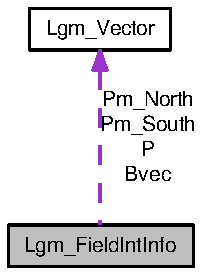
\includegraphics[width=134pt]{struct_lgm___field_int_info__coll__graph}
\end{center}
\end{figure}
\subsection*{Data Fields}
\begin{CompactItemize}
\item 
double \hyperlink{struct_lgm___field_int_info_869c8a1c2af0f48c6e871b08c13d2852}{KineticEnergy}
\item 
double \hyperlink{struct_lgm___field_int_info_c33418187547ea28dda7063924f34df6}{Mass}
\item 
double \hyperlink{struct_lgm___field_int_info_86da8321817d74036d3ff23e8643dc68}{PitchAngle}
\item 
\hyperlink{struct_lgm___vector}{Lgm\_\-Vector} \hyperlink{struct_lgm___field_int_info_a6b4371f4272ea673b10df3806973a78}{Pm\_\-South}
\item 
\hyperlink{struct_lgm___vector}{Lgm\_\-Vector} \hyperlink{struct_lgm___field_int_info_680815020ea7ef4edf84c04a0d7f1f20}{Pm\_\-North}
\item 
double \hyperlink{struct_lgm___field_int_info_8e90af044e680fe06a5f4745ead8b8d7}{Bm}
\item 
double \hyperlink{struct_lgm___field_int_info_91d445e45d4679505b1a9b5b7cde690c}{Sm\_\-South}
\item 
double \hyperlink{struct_lgm___field_int_info_e133118dcb4b4b581ae49086e9d16be3}{Sm\_\-North}
\item 
int \hyperlink{struct_lgm___field_int_info_52587930b11ea1eb053f0306dbc7973e}{FirstCall}
\item 
int \hyperlink{struct_lgm___field_int_info_5c3c9425f92b88e4cb8d1ee9129761d8}{n\_\-I\_\-integrand\_\-Calls}
\item 
int \hyperlink{struct_lgm___field_int_info_1f89d256729806dd1da1e84501e8d036}{n\_\-Sb\_\-integrand\_\-Calls}
\item 
double \hyperlink{struct_lgm___field_int_info_6aa234e3efbe6cefea9099de9f303f49}{epsabs}
\item 
double \hyperlink{struct_lgm___field_int_info_15d3900b8e4e4f00f7ae7d806828dd17}{epsrel}
\item 
double \hyperlink{struct_lgm___field_int_info_ceb7ba559344361c1beb271fc337896e}{s} \mbox{[}1000\mbox{]}
\item 
\hyperlink{struct_lgm___vector}{Lgm\_\-Vector} \hyperlink{struct_lgm___field_int_info_5ba0c6b33b6c0cb721daa1a92f0fdba2}{P} \mbox{[}1000\mbox{]}
\item 
\hyperlink{struct_lgm___vector}{Lgm\_\-Vector} \hyperlink{struct_lgm___field_int_info_861cd8f26a851c335b39a0f42a644bd8}{Bvec} \mbox{[}1000\mbox{]}
\item 
double \hyperlink{struct_lgm___field_int_info_6abcff3fdb33e77737583c51c10132e2}{Bmag} \mbox{[}1000\mbox{]}
\item 
int \hyperlink{struct_lgm___field_int_info_e64e724dd0713b2ba2fca5aedab3fd34}{nPnts}
\item 
int \hyperlink{struct_lgm___field_int_info_ef3011234df74566b679b46e01273bb7}{VerbosityLevel}
\end{CompactItemize}


\subsection{Detailed Description}


Definition at line 18 of file Lgm\_\-FieldIntInfo.h.

\subsection{Field Documentation}
\hypertarget{struct_lgm___field_int_info_869c8a1c2af0f48c6e871b08c13d2852}{
\index{Lgm\_\-FieldIntInfo@{Lgm\_\-FieldIntInfo}!KineticEnergy@{KineticEnergy}}
\index{KineticEnergy@{KineticEnergy}!Lgm_FieldIntInfo@{Lgm\_\-FieldIntInfo}}
\subsubsection[{KineticEnergy}]{\setlength{\rightskip}{0pt plus 5cm}double {\bf KineticEnergy}}}
\label{struct_lgm___field_int_info_869c8a1c2af0f48c6e871b08c13d2852}




Definition at line 20 of file Lgm\_\-FieldIntInfo.h.\hypertarget{struct_lgm___field_int_info_c33418187547ea28dda7063924f34df6}{
\index{Lgm\_\-FieldIntInfo@{Lgm\_\-FieldIntInfo}!Mass@{Mass}}
\index{Mass@{Mass}!Lgm_FieldIntInfo@{Lgm\_\-FieldIntInfo}}
\subsubsection[{Mass}]{\setlength{\rightskip}{0pt plus 5cm}double {\bf Mass}}}
\label{struct_lgm___field_int_info_c33418187547ea28dda7063924f34df6}




Definition at line 21 of file Lgm\_\-FieldIntInfo.h.\hypertarget{struct_lgm___field_int_info_86da8321817d74036d3ff23e8643dc68}{
\index{Lgm\_\-FieldIntInfo@{Lgm\_\-FieldIntInfo}!PitchAngle@{PitchAngle}}
\index{PitchAngle@{PitchAngle}!Lgm_FieldIntInfo@{Lgm\_\-FieldIntInfo}}
\subsubsection[{PitchAngle}]{\setlength{\rightskip}{0pt plus 5cm}double {\bf PitchAngle}}}
\label{struct_lgm___field_int_info_86da8321817d74036d3ff23e8643dc68}




Definition at line 22 of file Lgm\_\-FieldIntInfo.h.\hypertarget{struct_lgm___field_int_info_a6b4371f4272ea673b10df3806973a78}{
\index{Lgm\_\-FieldIntInfo@{Lgm\_\-FieldIntInfo}!Pm\_\-South@{Pm\_\-South}}
\index{Pm\_\-South@{Pm\_\-South}!Lgm_FieldIntInfo@{Lgm\_\-FieldIntInfo}}
\subsubsection[{Pm\_\-South}]{\setlength{\rightskip}{0pt plus 5cm}{\bf Lgm\_\-Vector} {\bf Pm\_\-South}}}
\label{struct_lgm___field_int_info_a6b4371f4272ea673b10df3806973a78}




Definition at line 24 of file Lgm\_\-FieldIntInfo.h.\hypertarget{struct_lgm___field_int_info_680815020ea7ef4edf84c04a0d7f1f20}{
\index{Lgm\_\-FieldIntInfo@{Lgm\_\-FieldIntInfo}!Pm\_\-North@{Pm\_\-North}}
\index{Pm\_\-North@{Pm\_\-North}!Lgm_FieldIntInfo@{Lgm\_\-FieldIntInfo}}
\subsubsection[{Pm\_\-North}]{\setlength{\rightskip}{0pt plus 5cm}{\bf Lgm\_\-Vector} {\bf Pm\_\-North}}}
\label{struct_lgm___field_int_info_680815020ea7ef4edf84c04a0d7f1f20}




Definition at line 25 of file Lgm\_\-FieldIntInfo.h.\hypertarget{struct_lgm___field_int_info_8e90af044e680fe06a5f4745ead8b8d7}{
\index{Lgm\_\-FieldIntInfo@{Lgm\_\-FieldIntInfo}!Bm@{Bm}}
\index{Bm@{Bm}!Lgm_FieldIntInfo@{Lgm\_\-FieldIntInfo}}
\subsubsection[{Bm}]{\setlength{\rightskip}{0pt plus 5cm}double {\bf Bm}}}
\label{struct_lgm___field_int_info_8e90af044e680fe06a5f4745ead8b8d7}




Definition at line 26 of file Lgm\_\-FieldIntInfo.h.\hypertarget{struct_lgm___field_int_info_91d445e45d4679505b1a9b5b7cde690c}{
\index{Lgm\_\-FieldIntInfo@{Lgm\_\-FieldIntInfo}!Sm\_\-South@{Sm\_\-South}}
\index{Sm\_\-South@{Sm\_\-South}!Lgm_FieldIntInfo@{Lgm\_\-FieldIntInfo}}
\subsubsection[{Sm\_\-South}]{\setlength{\rightskip}{0pt plus 5cm}double {\bf Sm\_\-South}}}
\label{struct_lgm___field_int_info_91d445e45d4679505b1a9b5b7cde690c}




Definition at line 26 of file Lgm\_\-FieldIntInfo.h.\hypertarget{struct_lgm___field_int_info_e133118dcb4b4b581ae49086e9d16be3}{
\index{Lgm\_\-FieldIntInfo@{Lgm\_\-FieldIntInfo}!Sm\_\-North@{Sm\_\-North}}
\index{Sm\_\-North@{Sm\_\-North}!Lgm_FieldIntInfo@{Lgm\_\-FieldIntInfo}}
\subsubsection[{Sm\_\-North}]{\setlength{\rightskip}{0pt plus 5cm}double {\bf Sm\_\-North}}}
\label{struct_lgm___field_int_info_e133118dcb4b4b581ae49086e9d16be3}




Definition at line 26 of file Lgm\_\-FieldIntInfo.h.\hypertarget{struct_lgm___field_int_info_52587930b11ea1eb053f0306dbc7973e}{
\index{Lgm\_\-FieldIntInfo@{Lgm\_\-FieldIntInfo}!FirstCall@{FirstCall}}
\index{FirstCall@{FirstCall}!Lgm_FieldIntInfo@{Lgm\_\-FieldIntInfo}}
\subsubsection[{FirstCall}]{\setlength{\rightskip}{0pt plus 5cm}int {\bf FirstCall}}}
\label{struct_lgm___field_int_info_52587930b11ea1eb053f0306dbc7973e}




Definition at line 27 of file Lgm\_\-FieldIntInfo.h.\hypertarget{struct_lgm___field_int_info_5c3c9425f92b88e4cb8d1ee9129761d8}{
\index{Lgm\_\-FieldIntInfo@{Lgm\_\-FieldIntInfo}!n\_\-I\_\-integrand\_\-Calls@{n\_\-I\_\-integrand\_\-Calls}}
\index{n\_\-I\_\-integrand\_\-Calls@{n\_\-I\_\-integrand\_\-Calls}!Lgm_FieldIntInfo@{Lgm\_\-FieldIntInfo}}
\subsubsection[{n\_\-I\_\-integrand\_\-Calls}]{\setlength{\rightskip}{0pt plus 5cm}int {\bf n\_\-I\_\-integrand\_\-Calls}}}
\label{struct_lgm___field_int_info_5c3c9425f92b88e4cb8d1ee9129761d8}




Definition at line 28 of file Lgm\_\-FieldIntInfo.h.\hypertarget{struct_lgm___field_int_info_1f89d256729806dd1da1e84501e8d036}{
\index{Lgm\_\-FieldIntInfo@{Lgm\_\-FieldIntInfo}!n\_\-Sb\_\-integrand\_\-Calls@{n\_\-Sb\_\-integrand\_\-Calls}}
\index{n\_\-Sb\_\-integrand\_\-Calls@{n\_\-Sb\_\-integrand\_\-Calls}!Lgm_FieldIntInfo@{Lgm\_\-FieldIntInfo}}
\subsubsection[{n\_\-Sb\_\-integrand\_\-Calls}]{\setlength{\rightskip}{0pt plus 5cm}int {\bf n\_\-Sb\_\-integrand\_\-Calls}}}
\label{struct_lgm___field_int_info_1f89d256729806dd1da1e84501e8d036}




Definition at line 29 of file Lgm\_\-FieldIntInfo.h.\hypertarget{struct_lgm___field_int_info_6aa234e3efbe6cefea9099de9f303f49}{
\index{Lgm\_\-FieldIntInfo@{Lgm\_\-FieldIntInfo}!epsabs@{epsabs}}
\index{epsabs@{epsabs}!Lgm_FieldIntInfo@{Lgm\_\-FieldIntInfo}}
\subsubsection[{epsabs}]{\setlength{\rightskip}{0pt plus 5cm}double {\bf epsabs}}}
\label{struct_lgm___field_int_info_6aa234e3efbe6cefea9099de9f303f49}




Definition at line 30 of file Lgm\_\-FieldIntInfo.h.\hypertarget{struct_lgm___field_int_info_15d3900b8e4e4f00f7ae7d806828dd17}{
\index{Lgm\_\-FieldIntInfo@{Lgm\_\-FieldIntInfo}!epsrel@{epsrel}}
\index{epsrel@{epsrel}!Lgm_FieldIntInfo@{Lgm\_\-FieldIntInfo}}
\subsubsection[{epsrel}]{\setlength{\rightskip}{0pt plus 5cm}double {\bf epsrel}}}
\label{struct_lgm___field_int_info_15d3900b8e4e4f00f7ae7d806828dd17}




Definition at line 30 of file Lgm\_\-FieldIntInfo.h.\hypertarget{struct_lgm___field_int_info_ceb7ba559344361c1beb271fc337896e}{
\index{Lgm\_\-FieldIntInfo@{Lgm\_\-FieldIntInfo}!s@{s}}
\index{s@{s}!Lgm_FieldIntInfo@{Lgm\_\-FieldIntInfo}}
\subsubsection[{s}]{\setlength{\rightskip}{0pt plus 5cm}double {\bf s}\mbox{[}1000\mbox{]}}}
\label{struct_lgm___field_int_info_ceb7ba559344361c1beb271fc337896e}




Definition at line 35 of file Lgm\_\-FieldIntInfo.h.\hypertarget{struct_lgm___field_int_info_5ba0c6b33b6c0cb721daa1a92f0fdba2}{
\index{Lgm\_\-FieldIntInfo@{Lgm\_\-FieldIntInfo}!P@{P}}
\index{P@{P}!Lgm_FieldIntInfo@{Lgm\_\-FieldIntInfo}}
\subsubsection[{P}]{\setlength{\rightskip}{0pt plus 5cm}{\bf Lgm\_\-Vector} {\bf P}\mbox{[}1000\mbox{]}}}
\label{struct_lgm___field_int_info_5ba0c6b33b6c0cb721daa1a92f0fdba2}




Definition at line 36 of file Lgm\_\-FieldIntInfo.h.\hypertarget{struct_lgm___field_int_info_861cd8f26a851c335b39a0f42a644bd8}{
\index{Lgm\_\-FieldIntInfo@{Lgm\_\-FieldIntInfo}!Bvec@{Bvec}}
\index{Bvec@{Bvec}!Lgm_FieldIntInfo@{Lgm\_\-FieldIntInfo}}
\subsubsection[{Bvec}]{\setlength{\rightskip}{0pt plus 5cm}{\bf Lgm\_\-Vector} {\bf Bvec}\mbox{[}1000\mbox{]}}}
\label{struct_lgm___field_int_info_861cd8f26a851c335b39a0f42a644bd8}




Definition at line 37 of file Lgm\_\-FieldIntInfo.h.\hypertarget{struct_lgm___field_int_info_6abcff3fdb33e77737583c51c10132e2}{
\index{Lgm\_\-FieldIntInfo@{Lgm\_\-FieldIntInfo}!Bmag@{Bmag}}
\index{Bmag@{Bmag}!Lgm_FieldIntInfo@{Lgm\_\-FieldIntInfo}}
\subsubsection[{Bmag}]{\setlength{\rightskip}{0pt plus 5cm}double {\bf Bmag}\mbox{[}1000\mbox{]}}}
\label{struct_lgm___field_int_info_6abcff3fdb33e77737583c51c10132e2}




Definition at line 38 of file Lgm\_\-FieldIntInfo.h.\hypertarget{struct_lgm___field_int_info_e64e724dd0713b2ba2fca5aedab3fd34}{
\index{Lgm\_\-FieldIntInfo@{Lgm\_\-FieldIntInfo}!nPnts@{nPnts}}
\index{nPnts@{nPnts}!Lgm_FieldIntInfo@{Lgm\_\-FieldIntInfo}}
\subsubsection[{nPnts}]{\setlength{\rightskip}{0pt plus 5cm}int {\bf nPnts}}}
\label{struct_lgm___field_int_info_e64e724dd0713b2ba2fca5aedab3fd34}




Definition at line 39 of file Lgm\_\-FieldIntInfo.h.\hypertarget{struct_lgm___field_int_info_ef3011234df74566b679b46e01273bb7}{
\index{Lgm\_\-FieldIntInfo@{Lgm\_\-FieldIntInfo}!VerbosityLevel@{VerbosityLevel}}
\index{VerbosityLevel@{VerbosityLevel}!Lgm_FieldIntInfo@{Lgm\_\-FieldIntInfo}}
\subsubsection[{VerbosityLevel}]{\setlength{\rightskip}{0pt plus 5cm}int {\bf VerbosityLevel}}}
\label{struct_lgm___field_int_info_ef3011234df74566b679b46e01273bb7}




Definition at line 45 of file Lgm\_\-FieldIntInfo.h.

The documentation for this struct was generated from the following file:\begin{CompactItemize}
\item 
/home/mgh/LanlGeoMag/libLanlGeoMag/Lgm/\hyperlink{_lgm___field_int_info_8h}{Lgm\_\-FieldIntInfo.h}\end{CompactItemize}

\hypertarget{struct_lgm___leap_seconds}{
\section{Lgm\_\-LeapSeconds Struct Reference}
\label{struct_lgm___leap_seconds}\index{Lgm\_\-LeapSeconds@{Lgm\_\-LeapSeconds}}
}
{\tt \#include $<$Lgm\_\-CTrans.h$>$}

\subsection*{Data Fields}
\begin{CompactItemize}
\item 
int \hyperlink{struct_lgm___leap_seconds_a3dde6cfdaff24850ad827b07a0730d7}{nLeapSecondDates}
\begin{CompactList}\small\item\em Number of leap second dates. \item\end{CompactList}\item 
long int $\ast$ \hyperlink{struct_lgm___leap_seconds_4369aebda8e4aea18cba6dc90d539dc7}{LeapSecondDates}
\begin{CompactList}\small\item\em Array for holdin the Dates on which leap seconds were added. \item\end{CompactList}\item 
double $\ast$ \hyperlink{struct_lgm___leap_seconds_e2bc1c43d2bc9b92f9558233db952daf}{LeapSecondJDs}
\begin{CompactList}\small\item\em Array for holdin the Julian Dates on which leap seconds were added. \item\end{CompactList}\item 
double $\ast$ \hyperlink{struct_lgm___leap_seconds_47824494de1cdaafed7bee00b27b27af}{LeapSeconds}
\begin{CompactList}\small\item\em The actual number of leap seconds that went into effect on the given date. \item\end{CompactList}\end{CompactItemize}


\subsection{Detailed Description}


Definition at line 420 of file Lgm\_\-CTrans.h.

\subsection{Field Documentation}
\hypertarget{struct_lgm___leap_seconds_a3dde6cfdaff24850ad827b07a0730d7}{
\index{Lgm\_\-LeapSeconds@{Lgm\_\-LeapSeconds}!nLeapSecondDates@{nLeapSecondDates}}
\index{nLeapSecondDates@{nLeapSecondDates}!Lgm_LeapSeconds@{Lgm\_\-LeapSeconds}}
\subsubsection[{nLeapSecondDates}]{\setlength{\rightskip}{0pt plus 5cm}int {\bf nLeapSecondDates}}}
\label{struct_lgm___leap_seconds_a3dde6cfdaff24850ad827b07a0730d7}


Number of leap second dates. 



Definition at line 422 of file Lgm\_\-CTrans.h.\hypertarget{struct_lgm___leap_seconds_4369aebda8e4aea18cba6dc90d539dc7}{
\index{Lgm\_\-LeapSeconds@{Lgm\_\-LeapSeconds}!LeapSecondDates@{LeapSecondDates}}
\index{LeapSecondDates@{LeapSecondDates}!Lgm_LeapSeconds@{Lgm\_\-LeapSeconds}}
\subsubsection[{LeapSecondDates}]{\setlength{\rightskip}{0pt plus 5cm}long int $\ast$ {\bf LeapSecondDates}}}
\label{struct_lgm___leap_seconds_4369aebda8e4aea18cba6dc90d539dc7}


Array for holdin the Dates on which leap seconds were added. 



Definition at line 424 of file Lgm\_\-CTrans.h.\hypertarget{struct_lgm___leap_seconds_e2bc1c43d2bc9b92f9558233db952daf}{
\index{Lgm\_\-LeapSeconds@{Lgm\_\-LeapSeconds}!LeapSecondJDs@{LeapSecondJDs}}
\index{LeapSecondJDs@{LeapSecondJDs}!Lgm_LeapSeconds@{Lgm\_\-LeapSeconds}}
\subsubsection[{LeapSecondJDs}]{\setlength{\rightskip}{0pt plus 5cm}double $\ast$ {\bf LeapSecondJDs}}}
\label{struct_lgm___leap_seconds_e2bc1c43d2bc9b92f9558233db952daf}


Array for holdin the Julian Dates on which leap seconds were added. 



Definition at line 426 of file Lgm\_\-CTrans.h.\hypertarget{struct_lgm___leap_seconds_47824494de1cdaafed7bee00b27b27af}{
\index{Lgm\_\-LeapSeconds@{Lgm\_\-LeapSeconds}!LeapSeconds@{LeapSeconds}}
\index{LeapSeconds@{LeapSeconds}!Lgm_LeapSeconds@{Lgm\_\-LeapSeconds}}
\subsubsection[{LeapSeconds}]{\setlength{\rightskip}{0pt plus 5cm}double $\ast$ {\bf LeapSeconds}}}
\label{struct_lgm___leap_seconds_47824494de1cdaafed7bee00b27b27af}


The actual number of leap seconds that went into effect on the given date. 



Definition at line 428 of file Lgm\_\-CTrans.h.

The documentation for this struct was generated from the following files:\begin{CompactItemize}
\item 
/home/mgh/LanlGeoMag/libLanlGeoMag/Lgm/\hyperlink{_lgm___c_trans_8h}{Lgm\_\-CTrans.h}\item 
/home/mgh/LanlGeoMag/libLanlGeoMag/Lgm/\hyperlink{_lgm___leap_seconds_8h}{Lgm\_\-LeapSeconds.h}\end{CompactItemize}

\hypertarget{struct_lgm___lstar_info}{
\section{Lgm\_\-LstarInfo Struct Reference}
\label{struct_lgm___lstar_info}\index{Lgm\_\-LstarInfo@{Lgm\_\-LstarInfo}}
}
{\tt \#include $<$Lgm\_\-LstarInfo.h$>$}

Collaboration diagram for Lgm\_\-LstarInfo:\nopagebreak
\begin{figure}[H]
\begin{center}
\leavevmode
\includegraphics[width=400pt]{struct_lgm___lstar_info__coll__graph}
\end{center}
\end{figure}
\subsection*{Data Fields}
\begin{CompactItemize}
\item 
double \hyperlink{struct_lgm___lstar_info_869c8a1c2af0f48c6e871b08c13d2852}{KineticEnergy}
\item 
double \hyperlink{struct_lgm___lstar_info_c33418187547ea28dda7063924f34df6}{Mass}
\item 
double \hyperlink{struct_lgm___lstar_info_86da8321817d74036d3ff23e8643dc68}{PitchAngle}
\item 
double \hyperlink{struct_lgm___lstar_info_5d743063aa757414e17e949240d3c85b}{LSimpleMax}
\item 
\hyperlink{struct_lgm___mag_model_info}{Lgm\_\-MagModelInfo} $\ast$ \hyperlink{struct_lgm___lstar_info_c8b439eddbb4183c79fe090c634587a5}{mInfo}
\item 
int \hyperlink{struct_lgm___lstar_info_5e915118a580b5fdd3fc46cb0a09d618}{SaveShellLines}
\item 
int \hyperlink{struct_lgm___lstar_info_09227be97e257b54115370b3a6a7068d}{nFieldPnts} \mbox{[}100\mbox{]}
\item 
double \hyperlink{struct_lgm___lstar_info_1afc9fdd1806999a43e3c0ca0e6f7439}{s\_\-gsm} \mbox{[}100\mbox{]}\mbox{[}1000\mbox{]}
\item 
double \hyperlink{struct_lgm___lstar_info_7863fc2c379717c21a5bb5e3f217a74b}{Bmag} \mbox{[}100\mbox{]}\mbox{[}1000\mbox{]}
\item 
double \hyperlink{struct_lgm___lstar_info_fc2724b1c578713a685b87b9e12ea4b0}{x\_\-gsm} \mbox{[}100\mbox{]}\mbox{[}1000\mbox{]}
\item 
double \hyperlink{struct_lgm___lstar_info_713bca9193697dece782322446d6bf4f}{y\_\-gsm} \mbox{[}100\mbox{]}\mbox{[}1000\mbox{]}
\item 
double \hyperlink{struct_lgm___lstar_info_42b27005ed6595929e25c1e9ca6b9f8d}{z\_\-gsm} \mbox{[}100\mbox{]}\mbox{[}1000\mbox{]}
\item 
int \hyperlink{struct_lgm___lstar_info_e64e724dd0713b2ba2fca5aedab3fd34}{nPnts}
\item 
double \hyperlink{struct_lgm___lstar_info_81220a2a156b6eaf6e17f742e55648e0}{MLT} \mbox{[}100\mbox{]}
\item 
double \hyperlink{struct_lgm___lstar_info_34853551c7862f1bca3adc0be7482483}{mlat} \mbox{[}100\mbox{]}
\item 
\hyperlink{struct_lgm___vector}{Lgm\_\-Vector} \hyperlink{struct_lgm___lstar_info_9548ca1b43dee446afddb58200852ac4}{Footprint\_\-Pn} \mbox{[}100\mbox{]}
\item 
\hyperlink{struct_lgm___vector}{Lgm\_\-Vector} \hyperlink{struct_lgm___lstar_info_cab1b2b38cdcb108925a62d5776ea71c}{Mirror\_\-Pn} \mbox{[}100\mbox{]}
\item 
\hyperlink{struct_lgm___vector}{Lgm\_\-Vector} \hyperlink{struct_lgm___lstar_info_ade743fcc24633af3a5485dc7a9d5147}{Footprint\_\-Ps} \mbox{[}100\mbox{]}
\item 
\hyperlink{struct_lgm___vector}{Lgm\_\-Vector} \hyperlink{struct_lgm___lstar_info_3b9e030b6e119c8e96b971ff682288c9}{Mirror\_\-Ps} \mbox{[}100\mbox{]}
\item 
double \hyperlink{struct_lgm___lstar_info_04ec246114a405539c0accd9be478347}{PhiVal} \mbox{[}100\mbox{]}
\item 
double \hyperlink{struct_lgm___lstar_info_d76bd4e5f331d6a1ddcaa1639fd68496}{AngularVelocity} \mbox{[}100\mbox{]}
\item 
double \hyperlink{struct_lgm___lstar_info_41ab61f1b0e2b2ebe5247fbbbdd57b0b}{I} \mbox{[}100\mbox{]}
\item 
int \hyperlink{struct_lgm___lstar_info_11528df252ee43e0e82ac6490020181f}{nSplnPnts}
\item 
double \hyperlink{struct_lgm___lstar_info_501f2c063215b27203462b91f615f570}{xa} \mbox{[}500\mbox{]}
\item 
double \hyperlink{struct_lgm___lstar_info_2186b66c32c372f89e9cd85d4e0e5bea}{ya} \mbox{[}500\mbox{]}
\item 
double \hyperlink{struct_lgm___lstar_info_4e6e2ef6cbd430bce10cbd07a1e6c045}{y2} \mbox{[}500\mbox{]}
\item 
double \hyperlink{struct_lgm___lstar_info_0701272ef4e36f8d410e1a99161361fe}{Phi}
\item 
gsl\_\-interp\_\-accel $\ast$ \hyperlink{struct_lgm___lstar_info_7c9a9e6523a7a6e67a5b349e772e3765}{acc}
\item 
gsl\_\-interp $\ast$ \hyperlink{struct_lgm___lstar_info_e44485025e16910b09a8c4e37b519bb1}{pspline}
\item 
int \hyperlink{struct_lgm___lstar_info_ef3011234df74566b679b46e01273bb7}{VerbosityLevel}
\item 
char \hyperlink{struct_lgm___lstar_info_4f91fd49adec5f649e536a8d0c61f15f}{PreStr} \mbox{[}64\mbox{]}
\item 
char \hyperlink{struct_lgm___lstar_info_450023a7fe05d37b7b67d03dc1efc7ba}{PostStr} \mbox{[}64\mbox{]}
\item 
double \hyperlink{struct_lgm___lstar_info_6ad8261bf3a41eb108787d3d924f5c45}{LS}
\item 
double \hyperlink{struct_lgm___lstar_info_c11d4471d4e71707da1bbfdce47da54c}{LS\_\-dip\_\-approx}
\item 
double \hyperlink{struct_lgm___lstar_info_881b139aff4cc429e41c7ec564d32840}{LS\_\-McIlwain\_\-M}
\item 
int \hyperlink{struct_lgm___lstar_info_742204794ea328ba293fe59cec79b990}{m}
\item 
double \hyperlink{struct_lgm___lstar_info_7b60b67e8a8714de350f686c14a6866e}{xma} \mbox{[}500\mbox{]}
\item 
double \hyperlink{struct_lgm___lstar_info_911c5b5fff6eb68546281d9a63610f81}{yma} \mbox{[}500\mbox{]}
\item 
double \hyperlink{struct_lgm___lstar_info_33c7d04ab4147ef8853fb6621a6a7456}{ym2} \mbox{[}500\mbox{]}
\item 
int \hyperlink{struct_lgm___lstar_info_9e239b576529625f9b2f05c84b12b4a9}{nParticles}
\item 
\hyperlink{struct_lgm___vector}{Lgm\_\-Vector} \hyperlink{struct_lgm___lstar_info_5ff4824ef9c331c0e8a9683e62de9e98}{Particles} \mbox{[}5000\mbox{]}
\end{CompactItemize}


\subsection{Detailed Description}


Definition at line 22 of file Lgm\_\-LstarInfo.h.

\subsection{Field Documentation}
\hypertarget{struct_lgm___lstar_info_869c8a1c2af0f48c6e871b08c13d2852}{
\index{Lgm\_\-LstarInfo@{Lgm\_\-LstarInfo}!KineticEnergy@{KineticEnergy}}
\index{KineticEnergy@{KineticEnergy}!Lgm_LstarInfo@{Lgm\_\-LstarInfo}}
\subsubsection[{KineticEnergy}]{\setlength{\rightskip}{0pt plus 5cm}double {\bf KineticEnergy}}}
\label{struct_lgm___lstar_info_869c8a1c2af0f48c6e871b08c13d2852}




Definition at line 24 of file Lgm\_\-LstarInfo.h.\hypertarget{struct_lgm___lstar_info_c33418187547ea28dda7063924f34df6}{
\index{Lgm\_\-LstarInfo@{Lgm\_\-LstarInfo}!Mass@{Mass}}
\index{Mass@{Mass}!Lgm_LstarInfo@{Lgm\_\-LstarInfo}}
\subsubsection[{Mass}]{\setlength{\rightskip}{0pt plus 5cm}double {\bf Mass}}}
\label{struct_lgm___lstar_info_c33418187547ea28dda7063924f34df6}




Definition at line 25 of file Lgm\_\-LstarInfo.h.\hypertarget{struct_lgm___lstar_info_86da8321817d74036d3ff23e8643dc68}{
\index{Lgm\_\-LstarInfo@{Lgm\_\-LstarInfo}!PitchAngle@{PitchAngle}}
\index{PitchAngle@{PitchAngle}!Lgm_LstarInfo@{Lgm\_\-LstarInfo}}
\subsubsection[{PitchAngle}]{\setlength{\rightskip}{0pt plus 5cm}double {\bf PitchAngle}}}
\label{struct_lgm___lstar_info_86da8321817d74036d3ff23e8643dc68}




Definition at line 26 of file Lgm\_\-LstarInfo.h.\hypertarget{struct_lgm___lstar_info_5d743063aa757414e17e949240d3c85b}{
\index{Lgm\_\-LstarInfo@{Lgm\_\-LstarInfo}!LSimpleMax@{LSimpleMax}}
\index{LSimpleMax@{LSimpleMax}!Lgm_LstarInfo@{Lgm\_\-LstarInfo}}
\subsubsection[{LSimpleMax}]{\setlength{\rightskip}{0pt plus 5cm}double {\bf LSimpleMax}}}
\label{struct_lgm___lstar_info_5d743063aa757414e17e949240d3c85b}




Definition at line 27 of file Lgm\_\-LstarInfo.h.\hypertarget{struct_lgm___lstar_info_c8b439eddbb4183c79fe090c634587a5}{
\index{Lgm\_\-LstarInfo@{Lgm\_\-LstarInfo}!mInfo@{mInfo}}
\index{mInfo@{mInfo}!Lgm_LstarInfo@{Lgm\_\-LstarInfo}}
\subsubsection[{mInfo}]{\setlength{\rightskip}{0pt plus 5cm}{\bf Lgm\_\-MagModelInfo}$\ast$ {\bf mInfo}}}
\label{struct_lgm___lstar_info_c8b439eddbb4183c79fe090c634587a5}




Definition at line 30 of file Lgm\_\-LstarInfo.h.\hypertarget{struct_lgm___lstar_info_5e915118a580b5fdd3fc46cb0a09d618}{
\index{Lgm\_\-LstarInfo@{Lgm\_\-LstarInfo}!SaveShellLines@{SaveShellLines}}
\index{SaveShellLines@{SaveShellLines}!Lgm_LstarInfo@{Lgm\_\-LstarInfo}}
\subsubsection[{SaveShellLines}]{\setlength{\rightskip}{0pt plus 5cm}int {\bf SaveShellLines}}}
\label{struct_lgm___lstar_info_5e915118a580b5fdd3fc46cb0a09d618}




Definition at line 35 of file Lgm\_\-LstarInfo.h.\hypertarget{struct_lgm___lstar_info_09227be97e257b54115370b3a6a7068d}{
\index{Lgm\_\-LstarInfo@{Lgm\_\-LstarInfo}!nFieldPnts@{nFieldPnts}}
\index{nFieldPnts@{nFieldPnts}!Lgm_LstarInfo@{Lgm\_\-LstarInfo}}
\subsubsection[{nFieldPnts}]{\setlength{\rightskip}{0pt plus 5cm}int {\bf nFieldPnts}\mbox{[}100\mbox{]}}}
\label{struct_lgm___lstar_info_09227be97e257b54115370b3a6a7068d}




Definition at line 36 of file Lgm\_\-LstarInfo.h.\hypertarget{struct_lgm___lstar_info_1afc9fdd1806999a43e3c0ca0e6f7439}{
\index{Lgm\_\-LstarInfo@{Lgm\_\-LstarInfo}!s\_\-gsm@{s\_\-gsm}}
\index{s\_\-gsm@{s\_\-gsm}!Lgm_LstarInfo@{Lgm\_\-LstarInfo}}
\subsubsection[{s\_\-gsm}]{\setlength{\rightskip}{0pt plus 5cm}double {\bf s\_\-gsm}\mbox{[}100\mbox{]}\mbox{[}1000\mbox{]}}}
\label{struct_lgm___lstar_info_1afc9fdd1806999a43e3c0ca0e6f7439}




Definition at line 37 of file Lgm\_\-LstarInfo.h.\hypertarget{struct_lgm___lstar_info_7863fc2c379717c21a5bb5e3f217a74b}{
\index{Lgm\_\-LstarInfo@{Lgm\_\-LstarInfo}!Bmag@{Bmag}}
\index{Bmag@{Bmag}!Lgm_LstarInfo@{Lgm\_\-LstarInfo}}
\subsubsection[{Bmag}]{\setlength{\rightskip}{0pt plus 5cm}double {\bf Bmag}\mbox{[}100\mbox{]}\mbox{[}1000\mbox{]}}}
\label{struct_lgm___lstar_info_7863fc2c379717c21a5bb5e3f217a74b}




Definition at line 38 of file Lgm\_\-LstarInfo.h.\hypertarget{struct_lgm___lstar_info_fc2724b1c578713a685b87b9e12ea4b0}{
\index{Lgm\_\-LstarInfo@{Lgm\_\-LstarInfo}!x\_\-gsm@{x\_\-gsm}}
\index{x\_\-gsm@{x\_\-gsm}!Lgm_LstarInfo@{Lgm\_\-LstarInfo}}
\subsubsection[{x\_\-gsm}]{\setlength{\rightskip}{0pt plus 5cm}double {\bf x\_\-gsm}\mbox{[}100\mbox{]}\mbox{[}1000\mbox{]}}}
\label{struct_lgm___lstar_info_fc2724b1c578713a685b87b9e12ea4b0}




Definition at line 39 of file Lgm\_\-LstarInfo.h.\hypertarget{struct_lgm___lstar_info_713bca9193697dece782322446d6bf4f}{
\index{Lgm\_\-LstarInfo@{Lgm\_\-LstarInfo}!y\_\-gsm@{y\_\-gsm}}
\index{y\_\-gsm@{y\_\-gsm}!Lgm_LstarInfo@{Lgm\_\-LstarInfo}}
\subsubsection[{y\_\-gsm}]{\setlength{\rightskip}{0pt plus 5cm}double {\bf y\_\-gsm}\mbox{[}100\mbox{]}\mbox{[}1000\mbox{]}}}
\label{struct_lgm___lstar_info_713bca9193697dece782322446d6bf4f}




Definition at line 40 of file Lgm\_\-LstarInfo.h.\hypertarget{struct_lgm___lstar_info_42b27005ed6595929e25c1e9ca6b9f8d}{
\index{Lgm\_\-LstarInfo@{Lgm\_\-LstarInfo}!z\_\-gsm@{z\_\-gsm}}
\index{z\_\-gsm@{z\_\-gsm}!Lgm_LstarInfo@{Lgm\_\-LstarInfo}}
\subsubsection[{z\_\-gsm}]{\setlength{\rightskip}{0pt plus 5cm}double {\bf z\_\-gsm}\mbox{[}100\mbox{]}\mbox{[}1000\mbox{]}}}
\label{struct_lgm___lstar_info_42b27005ed6595929e25c1e9ca6b9f8d}




Definition at line 41 of file Lgm\_\-LstarInfo.h.\hypertarget{struct_lgm___lstar_info_e64e724dd0713b2ba2fca5aedab3fd34}{
\index{Lgm\_\-LstarInfo@{Lgm\_\-LstarInfo}!nPnts@{nPnts}}
\index{nPnts@{nPnts}!Lgm_LstarInfo@{Lgm\_\-LstarInfo}}
\subsubsection[{nPnts}]{\setlength{\rightskip}{0pt plus 5cm}int {\bf nPnts}}}
\label{struct_lgm___lstar_info_e64e724dd0713b2ba2fca5aedab3fd34}




Definition at line 47 of file Lgm\_\-LstarInfo.h.\hypertarget{struct_lgm___lstar_info_81220a2a156b6eaf6e17f742e55648e0}{
\index{Lgm\_\-LstarInfo@{Lgm\_\-LstarInfo}!MLT@{MLT}}
\index{MLT@{MLT}!Lgm_LstarInfo@{Lgm\_\-LstarInfo}}
\subsubsection[{MLT}]{\setlength{\rightskip}{0pt plus 5cm}double {\bf MLT}\mbox{[}100\mbox{]}}}
\label{struct_lgm___lstar_info_81220a2a156b6eaf6e17f742e55648e0}




Definition at line 48 of file Lgm\_\-LstarInfo.h.\hypertarget{struct_lgm___lstar_info_34853551c7862f1bca3adc0be7482483}{
\index{Lgm\_\-LstarInfo@{Lgm\_\-LstarInfo}!mlat@{mlat}}
\index{mlat@{mlat}!Lgm_LstarInfo@{Lgm\_\-LstarInfo}}
\subsubsection[{mlat}]{\setlength{\rightskip}{0pt plus 5cm}double {\bf mlat}\mbox{[}100\mbox{]}}}
\label{struct_lgm___lstar_info_34853551c7862f1bca3adc0be7482483}




Definition at line 48 of file Lgm\_\-LstarInfo.h.\hypertarget{struct_lgm___lstar_info_9548ca1b43dee446afddb58200852ac4}{
\index{Lgm\_\-LstarInfo@{Lgm\_\-LstarInfo}!Footprint\_\-Pn@{Footprint\_\-Pn}}
\index{Footprint\_\-Pn@{Footprint\_\-Pn}!Lgm_LstarInfo@{Lgm\_\-LstarInfo}}
\subsubsection[{Footprint\_\-Pn}]{\setlength{\rightskip}{0pt plus 5cm}{\bf Lgm\_\-Vector} {\bf Footprint\_\-Pn}\mbox{[}100\mbox{]}}}
\label{struct_lgm___lstar_info_9548ca1b43dee446afddb58200852ac4}




Definition at line 49 of file Lgm\_\-LstarInfo.h.\hypertarget{struct_lgm___lstar_info_cab1b2b38cdcb108925a62d5776ea71c}{
\index{Lgm\_\-LstarInfo@{Lgm\_\-LstarInfo}!Mirror\_\-Pn@{Mirror\_\-Pn}}
\index{Mirror\_\-Pn@{Mirror\_\-Pn}!Lgm_LstarInfo@{Lgm\_\-LstarInfo}}
\subsubsection[{Mirror\_\-Pn}]{\setlength{\rightskip}{0pt plus 5cm}{\bf Lgm\_\-Vector} {\bf Mirror\_\-Pn}\mbox{[}100\mbox{]}}}
\label{struct_lgm___lstar_info_cab1b2b38cdcb108925a62d5776ea71c}




Definition at line 50 of file Lgm\_\-LstarInfo.h.\hypertarget{struct_lgm___lstar_info_ade743fcc24633af3a5485dc7a9d5147}{
\index{Lgm\_\-LstarInfo@{Lgm\_\-LstarInfo}!Footprint\_\-Ps@{Footprint\_\-Ps}}
\index{Footprint\_\-Ps@{Footprint\_\-Ps}!Lgm_LstarInfo@{Lgm\_\-LstarInfo}}
\subsubsection[{Footprint\_\-Ps}]{\setlength{\rightskip}{0pt plus 5cm}{\bf Lgm\_\-Vector} {\bf Footprint\_\-Ps}\mbox{[}100\mbox{]}}}
\label{struct_lgm___lstar_info_ade743fcc24633af3a5485dc7a9d5147}




Definition at line 51 of file Lgm\_\-LstarInfo.h.\hypertarget{struct_lgm___lstar_info_3b9e030b6e119c8e96b971ff682288c9}{
\index{Lgm\_\-LstarInfo@{Lgm\_\-LstarInfo}!Mirror\_\-Ps@{Mirror\_\-Ps}}
\index{Mirror\_\-Ps@{Mirror\_\-Ps}!Lgm_LstarInfo@{Lgm\_\-LstarInfo}}
\subsubsection[{Mirror\_\-Ps}]{\setlength{\rightskip}{0pt plus 5cm}{\bf Lgm\_\-Vector} {\bf Mirror\_\-Ps}\mbox{[}100\mbox{]}}}
\label{struct_lgm___lstar_info_3b9e030b6e119c8e96b971ff682288c9}




Definition at line 52 of file Lgm\_\-LstarInfo.h.\hypertarget{struct_lgm___lstar_info_04ec246114a405539c0accd9be478347}{
\index{Lgm\_\-LstarInfo@{Lgm\_\-LstarInfo}!PhiVal@{PhiVal}}
\index{PhiVal@{PhiVal}!Lgm_LstarInfo@{Lgm\_\-LstarInfo}}
\subsubsection[{PhiVal}]{\setlength{\rightskip}{0pt plus 5cm}double {\bf PhiVal}\mbox{[}100\mbox{]}}}
\label{struct_lgm___lstar_info_04ec246114a405539c0accd9be478347}




Definition at line 53 of file Lgm\_\-LstarInfo.h.\hypertarget{struct_lgm___lstar_info_d76bd4e5f331d6a1ddcaa1639fd68496}{
\index{Lgm\_\-LstarInfo@{Lgm\_\-LstarInfo}!AngularVelocity@{AngularVelocity}}
\index{AngularVelocity@{AngularVelocity}!Lgm_LstarInfo@{Lgm\_\-LstarInfo}}
\subsubsection[{AngularVelocity}]{\setlength{\rightskip}{0pt plus 5cm}double {\bf AngularVelocity}\mbox{[}100\mbox{]}}}
\label{struct_lgm___lstar_info_d76bd4e5f331d6a1ddcaa1639fd68496}




Definition at line 53 of file Lgm\_\-LstarInfo.h.\hypertarget{struct_lgm___lstar_info_41ab61f1b0e2b2ebe5247fbbbdd57b0b}{
\index{Lgm\_\-LstarInfo@{Lgm\_\-LstarInfo}!I@{I}}
\index{I@{I}!Lgm_LstarInfo@{Lgm\_\-LstarInfo}}
\subsubsection[{I}]{\setlength{\rightskip}{0pt plus 5cm}double {\bf I}\mbox{[}100\mbox{]}}}
\label{struct_lgm___lstar_info_41ab61f1b0e2b2ebe5247fbbbdd57b0b}




Definition at line 54 of file Lgm\_\-LstarInfo.h.\hypertarget{struct_lgm___lstar_info_11528df252ee43e0e82ac6490020181f}{
\index{Lgm\_\-LstarInfo@{Lgm\_\-LstarInfo}!nSplnPnts@{nSplnPnts}}
\index{nSplnPnts@{nSplnPnts}!Lgm_LstarInfo@{Lgm\_\-LstarInfo}}
\subsubsection[{nSplnPnts}]{\setlength{\rightskip}{0pt plus 5cm}int {\bf nSplnPnts}}}
\label{struct_lgm___lstar_info_11528df252ee43e0e82ac6490020181f}




Definition at line 56 of file Lgm\_\-LstarInfo.h.\hypertarget{struct_lgm___lstar_info_501f2c063215b27203462b91f615f570}{
\index{Lgm\_\-LstarInfo@{Lgm\_\-LstarInfo}!xa@{xa}}
\index{xa@{xa}!Lgm_LstarInfo@{Lgm\_\-LstarInfo}}
\subsubsection[{xa}]{\setlength{\rightskip}{0pt plus 5cm}double {\bf xa}\mbox{[}500\mbox{]}}}
\label{struct_lgm___lstar_info_501f2c063215b27203462b91f615f570}




Definition at line 57 of file Lgm\_\-LstarInfo.h.\hypertarget{struct_lgm___lstar_info_2186b66c32c372f89e9cd85d4e0e5bea}{
\index{Lgm\_\-LstarInfo@{Lgm\_\-LstarInfo}!ya@{ya}}
\index{ya@{ya}!Lgm_LstarInfo@{Lgm\_\-LstarInfo}}
\subsubsection[{ya}]{\setlength{\rightskip}{0pt plus 5cm}double {\bf ya}\mbox{[}500\mbox{]}}}
\label{struct_lgm___lstar_info_2186b66c32c372f89e9cd85d4e0e5bea}




Definition at line 57 of file Lgm\_\-LstarInfo.h.\hypertarget{struct_lgm___lstar_info_4e6e2ef6cbd430bce10cbd07a1e6c045}{
\index{Lgm\_\-LstarInfo@{Lgm\_\-LstarInfo}!y2@{y2}}
\index{y2@{y2}!Lgm_LstarInfo@{Lgm\_\-LstarInfo}}
\subsubsection[{y2}]{\setlength{\rightskip}{0pt plus 5cm}double {\bf y2}\mbox{[}500\mbox{]}}}
\label{struct_lgm___lstar_info_4e6e2ef6cbd430bce10cbd07a1e6c045}




Definition at line 57 of file Lgm\_\-LstarInfo.h.\hypertarget{struct_lgm___lstar_info_0701272ef4e36f8d410e1a99161361fe}{
\index{Lgm\_\-LstarInfo@{Lgm\_\-LstarInfo}!Phi@{Phi}}
\index{Phi@{Phi}!Lgm_LstarInfo@{Lgm\_\-LstarInfo}}
\subsubsection[{Phi}]{\setlength{\rightskip}{0pt plus 5cm}double {\bf Phi}}}
\label{struct_lgm___lstar_info_0701272ef4e36f8d410e1a99161361fe}




Definition at line 59 of file Lgm\_\-LstarInfo.h.\hypertarget{struct_lgm___lstar_info_7c9a9e6523a7a6e67a5b349e772e3765}{
\index{Lgm\_\-LstarInfo@{Lgm\_\-LstarInfo}!acc@{acc}}
\index{acc@{acc}!Lgm_LstarInfo@{Lgm\_\-LstarInfo}}
\subsubsection[{acc}]{\setlength{\rightskip}{0pt plus 5cm}gsl\_\-interp\_\-accel$\ast$ {\bf acc}}}
\label{struct_lgm___lstar_info_7c9a9e6523a7a6e67a5b349e772e3765}




Definition at line 61 of file Lgm\_\-LstarInfo.h.\hypertarget{struct_lgm___lstar_info_e44485025e16910b09a8c4e37b519bb1}{
\index{Lgm\_\-LstarInfo@{Lgm\_\-LstarInfo}!pspline@{pspline}}
\index{pspline@{pspline}!Lgm_LstarInfo@{Lgm\_\-LstarInfo}}
\subsubsection[{pspline}]{\setlength{\rightskip}{0pt plus 5cm}gsl\_\-interp$\ast$ {\bf pspline}}}
\label{struct_lgm___lstar_info_e44485025e16910b09a8c4e37b519bb1}




Definition at line 62 of file Lgm\_\-LstarInfo.h.\hypertarget{struct_lgm___lstar_info_ef3011234df74566b679b46e01273bb7}{
\index{Lgm\_\-LstarInfo@{Lgm\_\-LstarInfo}!VerbosityLevel@{VerbosityLevel}}
\index{VerbosityLevel@{VerbosityLevel}!Lgm_LstarInfo@{Lgm\_\-LstarInfo}}
\subsubsection[{VerbosityLevel}]{\setlength{\rightskip}{0pt plus 5cm}int {\bf VerbosityLevel}}}
\label{struct_lgm___lstar_info_ef3011234df74566b679b46e01273bb7}




Definition at line 69 of file Lgm\_\-LstarInfo.h.\hypertarget{struct_lgm___lstar_info_4f91fd49adec5f649e536a8d0c61f15f}{
\index{Lgm\_\-LstarInfo@{Lgm\_\-LstarInfo}!PreStr@{PreStr}}
\index{PreStr@{PreStr}!Lgm_LstarInfo@{Lgm\_\-LstarInfo}}
\subsubsection[{PreStr}]{\setlength{\rightskip}{0pt plus 5cm}char {\bf PreStr}\mbox{[}64\mbox{]}}}
\label{struct_lgm___lstar_info_4f91fd49adec5f649e536a8d0c61f15f}




Definition at line 70 of file Lgm\_\-LstarInfo.h.\hypertarget{struct_lgm___lstar_info_450023a7fe05d37b7b67d03dc1efc7ba}{
\index{Lgm\_\-LstarInfo@{Lgm\_\-LstarInfo}!PostStr@{PostStr}}
\index{PostStr@{PostStr}!Lgm_LstarInfo@{Lgm\_\-LstarInfo}}
\subsubsection[{PostStr}]{\setlength{\rightskip}{0pt plus 5cm}char {\bf PostStr}\mbox{[}64\mbox{]}}}
\label{struct_lgm___lstar_info_450023a7fe05d37b7b67d03dc1efc7ba}




Definition at line 70 of file Lgm\_\-LstarInfo.h.\hypertarget{struct_lgm___lstar_info_6ad8261bf3a41eb108787d3d924f5c45}{
\index{Lgm\_\-LstarInfo@{Lgm\_\-LstarInfo}!LS@{LS}}
\index{LS@{LS}!Lgm_LstarInfo@{Lgm\_\-LstarInfo}}
\subsubsection[{LS}]{\setlength{\rightskip}{0pt plus 5cm}double {\bf LS}}}
\label{struct_lgm___lstar_info_6ad8261bf3a41eb108787d3d924f5c45}




Definition at line 72 of file Lgm\_\-LstarInfo.h.\hypertarget{struct_lgm___lstar_info_c11d4471d4e71707da1bbfdce47da54c}{
\index{Lgm\_\-LstarInfo@{Lgm\_\-LstarInfo}!LS\_\-dip\_\-approx@{LS\_\-dip\_\-approx}}
\index{LS\_\-dip\_\-approx@{LS\_\-dip\_\-approx}!Lgm_LstarInfo@{Lgm\_\-LstarInfo}}
\subsubsection[{LS\_\-dip\_\-approx}]{\setlength{\rightskip}{0pt plus 5cm}double {\bf LS\_\-dip\_\-approx}}}
\label{struct_lgm___lstar_info_c11d4471d4e71707da1bbfdce47da54c}




Definition at line 73 of file Lgm\_\-LstarInfo.h.\hypertarget{struct_lgm___lstar_info_881b139aff4cc429e41c7ec564d32840}{
\index{Lgm\_\-LstarInfo@{Lgm\_\-LstarInfo}!LS\_\-McIlwain\_\-M@{LS\_\-McIlwain\_\-M}}
\index{LS\_\-McIlwain\_\-M@{LS\_\-McIlwain\_\-M}!Lgm_LstarInfo@{Lgm\_\-LstarInfo}}
\subsubsection[{LS\_\-McIlwain\_\-M}]{\setlength{\rightskip}{0pt plus 5cm}double {\bf LS\_\-McIlwain\_\-M}}}
\label{struct_lgm___lstar_info_881b139aff4cc429e41c7ec564d32840}




Definition at line 74 of file Lgm\_\-LstarInfo.h.\hypertarget{struct_lgm___lstar_info_742204794ea328ba293fe59cec79b990}{
\index{Lgm\_\-LstarInfo@{Lgm\_\-LstarInfo}!m@{m}}
\index{m@{m}!Lgm_LstarInfo@{Lgm\_\-LstarInfo}}
\subsubsection[{m}]{\setlength{\rightskip}{0pt plus 5cm}int {\bf m}}}
\label{struct_lgm___lstar_info_742204794ea328ba293fe59cec79b990}




Definition at line 76 of file Lgm\_\-LstarInfo.h.\hypertarget{struct_lgm___lstar_info_7b60b67e8a8714de350f686c14a6866e}{
\index{Lgm\_\-LstarInfo@{Lgm\_\-LstarInfo}!xma@{xma}}
\index{xma@{xma}!Lgm_LstarInfo@{Lgm\_\-LstarInfo}}
\subsubsection[{xma}]{\setlength{\rightskip}{0pt plus 5cm}double {\bf xma}\mbox{[}500\mbox{]}}}
\label{struct_lgm___lstar_info_7b60b67e8a8714de350f686c14a6866e}




Definition at line 77 of file Lgm\_\-LstarInfo.h.\hypertarget{struct_lgm___lstar_info_911c5b5fff6eb68546281d9a63610f81}{
\index{Lgm\_\-LstarInfo@{Lgm\_\-LstarInfo}!yma@{yma}}
\index{yma@{yma}!Lgm_LstarInfo@{Lgm\_\-LstarInfo}}
\subsubsection[{yma}]{\setlength{\rightskip}{0pt plus 5cm}double {\bf yma}\mbox{[}500\mbox{]}}}
\label{struct_lgm___lstar_info_911c5b5fff6eb68546281d9a63610f81}




Definition at line 77 of file Lgm\_\-LstarInfo.h.\hypertarget{struct_lgm___lstar_info_33c7d04ab4147ef8853fb6621a6a7456}{
\index{Lgm\_\-LstarInfo@{Lgm\_\-LstarInfo}!ym2@{ym2}}
\index{ym2@{ym2}!Lgm_LstarInfo@{Lgm\_\-LstarInfo}}
\subsubsection[{ym2}]{\setlength{\rightskip}{0pt plus 5cm}double {\bf ym2}\mbox{[}500\mbox{]}}}
\label{struct_lgm___lstar_info_33c7d04ab4147ef8853fb6621a6a7456}




Definition at line 77 of file Lgm\_\-LstarInfo.h.\hypertarget{struct_lgm___lstar_info_9e239b576529625f9b2f05c84b12b4a9}{
\index{Lgm\_\-LstarInfo@{Lgm\_\-LstarInfo}!nParticles@{nParticles}}
\index{nParticles@{nParticles}!Lgm_LstarInfo@{Lgm\_\-LstarInfo}}
\subsubsection[{nParticles}]{\setlength{\rightskip}{0pt plus 5cm}int {\bf nParticles}}}
\label{struct_lgm___lstar_info_9e239b576529625f9b2f05c84b12b4a9}




Definition at line 84 of file Lgm\_\-LstarInfo.h.\hypertarget{struct_lgm___lstar_info_5ff4824ef9c331c0e8a9683e62de9e98}{
\index{Lgm\_\-LstarInfo@{Lgm\_\-LstarInfo}!Particles@{Particles}}
\index{Particles@{Particles}!Lgm_LstarInfo@{Lgm\_\-LstarInfo}}
\subsubsection[{Particles}]{\setlength{\rightskip}{0pt plus 5cm}{\bf Lgm\_\-Vector} {\bf Particles}\mbox{[}5000\mbox{]}}}
\label{struct_lgm___lstar_info_5ff4824ef9c331c0e8a9683e62de9e98}




Definition at line 85 of file Lgm\_\-LstarInfo.h.

The documentation for this struct was generated from the following file:\begin{CompactItemize}
\item 
/home/mgh/LanlGeoMag/libLanlGeoMag/Lgm/\hyperlink{_lgm___lstar_info_8h}{Lgm\_\-LstarInfo.h}\end{CompactItemize}

\hypertarget{struct_lgm___mag_ephem_info}{
\section{Lgm\_\-MagEphemInfo Struct Reference}
\label{struct_lgm___mag_ephem_info}\index{Lgm\_\-MagEphemInfo@{Lgm\_\-MagEphemInfo}}
}
{\tt \#include $<$Lgm\_\-MagEphemInfo.h$>$}

Collaboration diagram for Lgm\_\-MagEphemInfo:\nopagebreak
\begin{figure}[H]
\begin{center}
\leavevmode
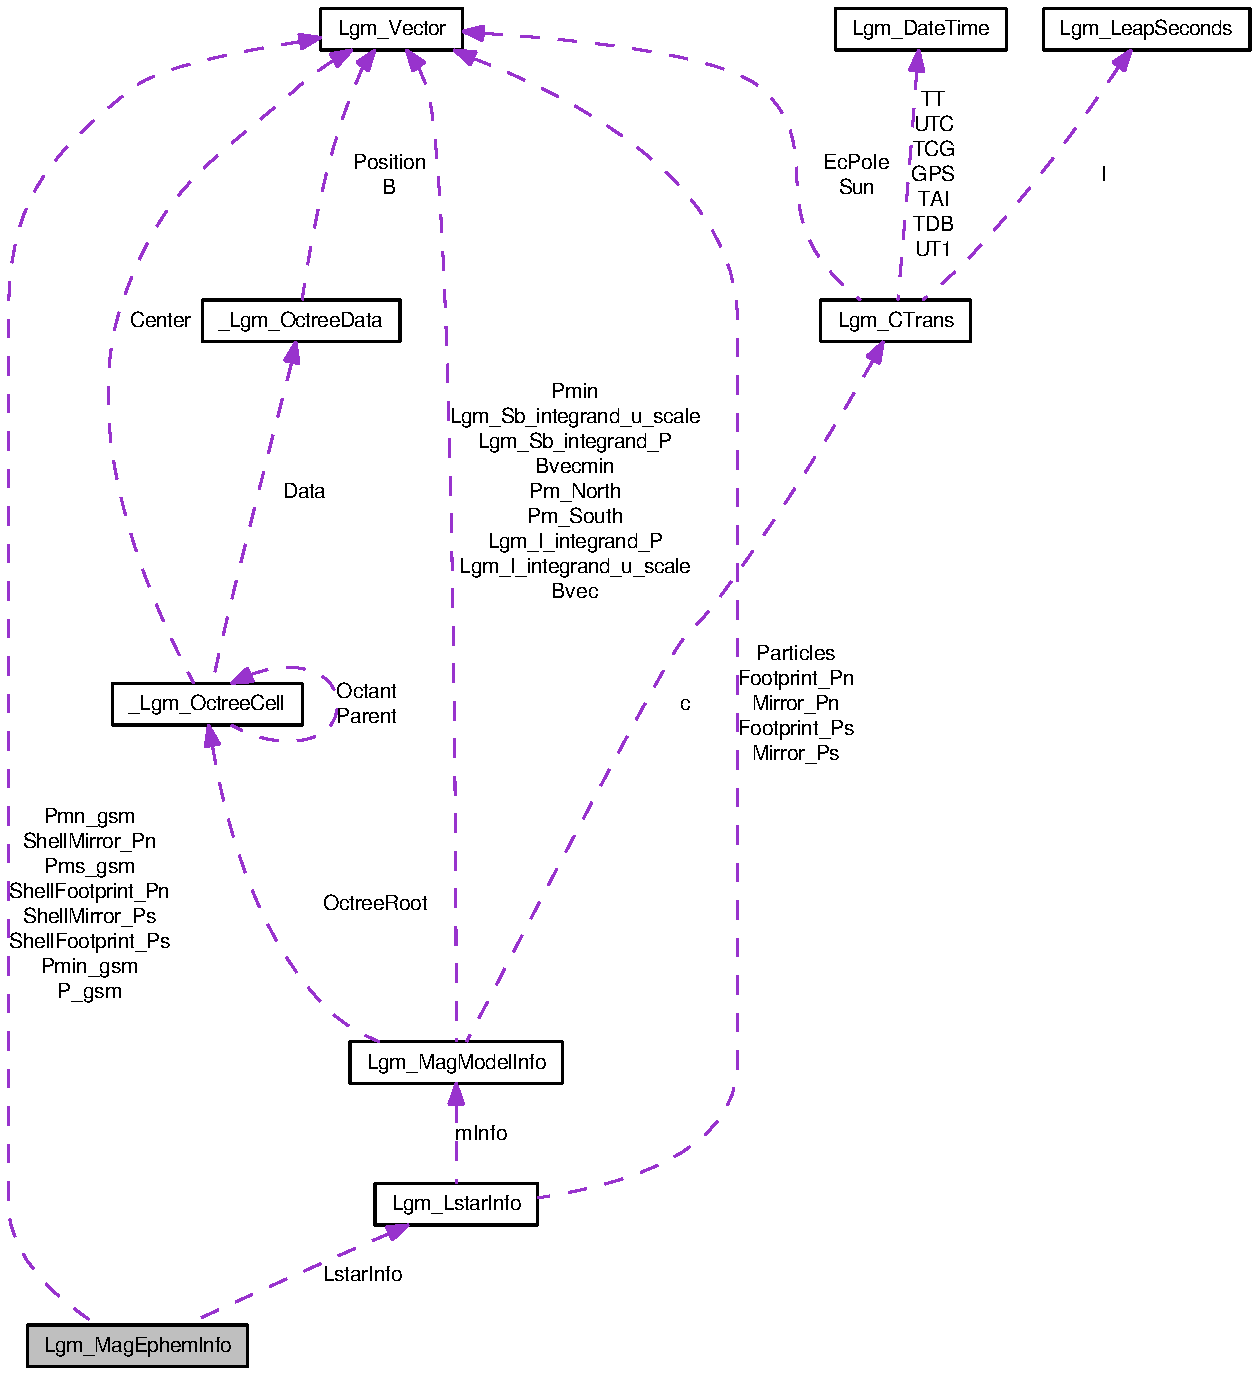
\includegraphics[width=400pt]{struct_lgm___mag_ephem_info__coll__graph}
\end{center}
\end{figure}
\subsection*{Data Fields}
\begin{CompactItemize}
\item 
\hyperlink{struct_lgm___lstar_info}{Lgm\_\-LstarInfo} $\ast$ \hyperlink{struct_lgm___mag_ephem_info_e0b196f79d448339982446d78890b87f}{LstarInfo}
\item 
int \hyperlink{struct_lgm___mag_ephem_info_8a900c463a0e976afa63d5736adbe8df}{LstarQuality}
\item 
int \hyperlink{struct_lgm___mag_ephem_info_5e915118a580b5fdd3fc46cb0a09d618}{SaveShellLines}
\item 
long int \hyperlink{struct_lgm___mag_ephem_info_8c1b7b17183e48a6fafaf6302e1b1da9}{Date}
\item 
double \hyperlink{struct_lgm___mag_ephem_info_4eccefabe940625eb9277991aa138a38}{UTC}
\item 
double \hyperlink{struct_lgm___mag_ephem_info_0db4289c0b4f63b151634b17a1718879}{Lat}
\item 
double \hyperlink{struct_lgm___mag_ephem_info_19c0faefc29efbada475c057d15844d6}{Lon}
\item 
double \hyperlink{struct_lgm___mag_ephem_info_860bef50013f57ab1a6437b7986a9487}{Rad}
\item 
\hyperlink{struct_lgm___vector}{Lgm\_\-Vector} \hyperlink{struct_lgm___mag_ephem_info_8a1a3f856fc793f9b4289bbf1d4c7f2f}{P\_\-gsm}
\item 
double \hyperlink{struct_lgm___mag_ephem_info_df085adbf76beb194ac436d42cd1d725}{B}
\item 
\hyperlink{struct_lgm___vector}{Lgm\_\-Vector} \hyperlink{struct_lgm___mag_ephem_info_da6476a5f53c9e2d9ac6f1b1b28a37b3}{Pmin\_\-gsm}
\item 
double \hyperlink{struct_lgm___mag_ephem_info_2ac3a99381d281d4caabf024a33f0b31}{Bmin}
\item 
int \hyperlink{struct_lgm___mag_ephem_info_beeccfbf7295d0c631353a9159972a74}{UseInterpRoutines}
\item 
int \hyperlink{struct_lgm___mag_ephem_info_b434059765e60f2934e7de8fe5eb50db}{nAlpha}
\item 
double \hyperlink{struct_lgm___mag_ephem_info_0083768551a2459ebaafb84f97c4decd}{Alpha} \mbox{[}MAX\_\-PITCH\_\-ANGLES\mbox{]}
\item 
\hyperlink{struct_lgm___vector}{Lgm\_\-Vector} \hyperlink{struct_lgm___mag_ephem_info_07d64e5d5028ce92c07e7b9f8a62aed0}{Pmn\_\-gsm} \mbox{[}MAX\_\-PITCH\_\-ANGLES\mbox{]}
\item 
\hyperlink{struct_lgm___vector}{Lgm\_\-Vector} \hyperlink{struct_lgm___mag_ephem_info_1d78a2b78227bd683d37e3b7eee614e9}{Pms\_\-gsm} \mbox{[}MAX\_\-PITCH\_\-ANGLES\mbox{]}
\item 
double \hyperlink{struct_lgm___mag_ephem_info_58b19efd51438b84ace93c628b985f64}{Bm} \mbox{[}MAX\_\-PITCH\_\-ANGLES\mbox{]}
\item 
double \hyperlink{struct_lgm___mag_ephem_info_f7c4c1569cb66f578b4bdef738b7e920}{I} \mbox{[}MAX\_\-PITCH\_\-ANGLES\mbox{]}
\item 
double \hyperlink{struct_lgm___mag_ephem_info_b7e342e135c0c1f98b60578a6accaa87}{Sb} \mbox{[}MAX\_\-PITCH\_\-ANGLES\mbox{]}
\item 
double \hyperlink{struct_lgm___mag_ephem_info_002672c07e6566f1824fb7d9f81228a2}{Tb} \mbox{[}MAX\_\-PITCH\_\-ANGLES\mbox{]}
\item 
double \hyperlink{struct_lgm___mag_ephem_info_2fc48ca4fe570dffe16ef8e235b572a2}{K} \mbox{[}MAX\_\-PITCH\_\-ANGLES\mbox{]}
\item 
int \hyperlink{struct_lgm___mag_ephem_info_7209f8815fcdddcb3100909e58729ae7}{nShellPoints} \mbox{[}MAX\_\-PITCH\_\-ANGLES\mbox{]}
\item 
\hyperlink{struct_lgm___vector}{Lgm\_\-Vector} \hyperlink{struct_lgm___mag_ephem_info_6476b5f20fa612531c2feca70655d947}{ShellFootprint\_\-Pn} \mbox{[}MAX\_\-PITCH\_\-ANGLES\mbox{]}\mbox{[}100\mbox{]}
\item 
\hyperlink{struct_lgm___vector}{Lgm\_\-Vector} \hyperlink{struct_lgm___mag_ephem_info_df864bbb783467664daaa3f072931827}{ShellFootprint\_\-Ps} \mbox{[}MAX\_\-PITCH\_\-ANGLES\mbox{]}\mbox{[}100\mbox{]}
\item 
\hyperlink{struct_lgm___vector}{Lgm\_\-Vector} \hyperlink{struct_lgm___mag_ephem_info_77f62c23ad73c46d65a58f3bd4df0007}{ShellMirror\_\-Pn} \mbox{[}MAX\_\-PITCH\_\-ANGLES\mbox{]}\mbox{[}100\mbox{]}
\item 
\hyperlink{struct_lgm___vector}{Lgm\_\-Vector} \hyperlink{struct_lgm___mag_ephem_info_f553d1e4efe198e474d5a38de0c6da91}{ShellMirror\_\-Ps} \mbox{[}MAX\_\-PITCH\_\-ANGLES\mbox{]}\mbox{[}100\mbox{]}
\item 
double \hyperlink{struct_lgm___mag_ephem_info_73c4025c84afef4f83812e9a70b69a72}{ShellMirror\_\-Sn} \mbox{[}MAX\_\-PITCH\_\-ANGLES\mbox{]}\mbox{[}100\mbox{]}
\item 
double \hyperlink{struct_lgm___mag_ephem_info_79d06251c694db0e26c64222f2078419}{ShellMirror\_\-Ss} \mbox{[}MAX\_\-PITCH\_\-ANGLES\mbox{]}\mbox{[}100\mbox{]}
\item 
double \hyperlink{struct_lgm___mag_ephem_info_9a29671c7d92f4a6fbbbf4caf6350b62}{ShellI} \mbox{[}MAX\_\-PITCH\_\-ANGLES\mbox{]}\mbox{[}100\mbox{]}
\item 
int \hyperlink{struct_lgm___mag_ephem_info_29cbea496fb314d5b004dd444cbe23a8}{nFieldPnts} \mbox{[}MAX\_\-PITCH\_\-ANGLES\mbox{]}\mbox{[}48\mbox{]}
\item 
double \hyperlink{struct_lgm___mag_ephem_info_fbd0f4250a5230950a688aa5fde2b8bc}{s\_\-gsm} \mbox{[}MAX\_\-PITCH\_\-ANGLES\mbox{]}\mbox{[}48\mbox{]}\mbox{[}1000\mbox{]}
\item 
double \hyperlink{struct_lgm___mag_ephem_info_8b01c6142170f19b03a8dc496b9a3678}{Bmag} \mbox{[}MAX\_\-PITCH\_\-ANGLES\mbox{]}\mbox{[}48\mbox{]}\mbox{[}1000\mbox{]}
\item 
double \hyperlink{struct_lgm___mag_ephem_info_59fdcbbc8f28e0dca963bdd893643827}{x\_\-gsm} \mbox{[}MAX\_\-PITCH\_\-ANGLES\mbox{]}\mbox{[}48\mbox{]}\mbox{[}1000\mbox{]}
\item 
double \hyperlink{struct_lgm___mag_ephem_info_2f086d0ae7b5e1afb9e95b5194ea3d84}{y\_\-gsm} \mbox{[}MAX\_\-PITCH\_\-ANGLES\mbox{]}\mbox{[}48\mbox{]}\mbox{[}1000\mbox{]}
\item 
double \hyperlink{struct_lgm___mag_ephem_info_604bb35325e4cdfd52be2d5d96fedc49}{z\_\-gsm} \mbox{[}MAX\_\-PITCH\_\-ANGLES\mbox{]}\mbox{[}48\mbox{]}\mbox{[}1000\mbox{]}
\item 
double \hyperlink{struct_lgm___mag_ephem_info_a63b377115bfe79515e2097f32738f8b}{Mcurr}
\item 
double \hyperlink{struct_lgm___mag_ephem_info_48f2de795abc764c809248272a03adbf}{Mref}
\item 
double \hyperlink{struct_lgm___mag_ephem_info_8cd747b5ee4d9da03a9ff039258c4df6}{Mused}
\item 
double \hyperlink{struct_lgm___mag_ephem_info_0c60b8e8cbed91a6659e978d407946c6}{LHilton} \mbox{[}MAX\_\-PITCH\_\-ANGLES\mbox{]}
\item 
double \hyperlink{struct_lgm___mag_ephem_info_ef38c562bbdfde054d2171e8183bac95}{LMcIlwain} \mbox{[}MAX\_\-PITCH\_\-ANGLES\mbox{]}
\item 
double \hyperlink{struct_lgm___mag_ephem_info_eb65115ebb3c6fc78a0250c76c345475}{Lstar} \mbox{[}MAX\_\-PITCH\_\-ANGLES\mbox{]}
\end{CompactItemize}


\subsection{Detailed Description}


Definition at line 15 of file Lgm\_\-MagEphemInfo.h.

\subsection{Field Documentation}
\hypertarget{struct_lgm___mag_ephem_info_e0b196f79d448339982446d78890b87f}{
\index{Lgm\_\-MagEphemInfo@{Lgm\_\-MagEphemInfo}!LstarInfo@{LstarInfo}}
\index{LstarInfo@{LstarInfo}!Lgm_MagEphemInfo@{Lgm\_\-MagEphemInfo}}
\subsubsection[{LstarInfo}]{\setlength{\rightskip}{0pt plus 5cm}{\bf Lgm\_\-LstarInfo}$\ast$ {\bf LstarInfo}}}
\label{struct_lgm___mag_ephem_info_e0b196f79d448339982446d78890b87f}




Definition at line 17 of file Lgm\_\-MagEphemInfo.h.\hypertarget{struct_lgm___mag_ephem_info_8a900c463a0e976afa63d5736adbe8df}{
\index{Lgm\_\-MagEphemInfo@{Lgm\_\-MagEphemInfo}!LstarQuality@{LstarQuality}}
\index{LstarQuality@{LstarQuality}!Lgm_MagEphemInfo@{Lgm\_\-MagEphemInfo}}
\subsubsection[{LstarQuality}]{\setlength{\rightskip}{0pt plus 5cm}int {\bf LstarQuality}}}
\label{struct_lgm___mag_ephem_info_8a900c463a0e976afa63d5736adbe8df}




Definition at line 18 of file Lgm\_\-MagEphemInfo.h.\hypertarget{struct_lgm___mag_ephem_info_5e915118a580b5fdd3fc46cb0a09d618}{
\index{Lgm\_\-MagEphemInfo@{Lgm\_\-MagEphemInfo}!SaveShellLines@{SaveShellLines}}
\index{SaveShellLines@{SaveShellLines}!Lgm_MagEphemInfo@{Lgm\_\-MagEphemInfo}}
\subsubsection[{SaveShellLines}]{\setlength{\rightskip}{0pt plus 5cm}int {\bf SaveShellLines}}}
\label{struct_lgm___mag_ephem_info_5e915118a580b5fdd3fc46cb0a09d618}




Definition at line 19 of file Lgm\_\-MagEphemInfo.h.\hypertarget{struct_lgm___mag_ephem_info_8c1b7b17183e48a6fafaf6302e1b1da9}{
\index{Lgm\_\-MagEphemInfo@{Lgm\_\-MagEphemInfo}!Date@{Date}}
\index{Date@{Date}!Lgm_MagEphemInfo@{Lgm\_\-MagEphemInfo}}
\subsubsection[{Date}]{\setlength{\rightskip}{0pt plus 5cm}long int {\bf Date}}}
\label{struct_lgm___mag_ephem_info_8c1b7b17183e48a6fafaf6302e1b1da9}




Definition at line 21 of file Lgm\_\-MagEphemInfo.h.\hypertarget{struct_lgm___mag_ephem_info_4eccefabe940625eb9277991aa138a38}{
\index{Lgm\_\-MagEphemInfo@{Lgm\_\-MagEphemInfo}!UTC@{UTC}}
\index{UTC@{UTC}!Lgm_MagEphemInfo@{Lgm\_\-MagEphemInfo}}
\subsubsection[{UTC}]{\setlength{\rightskip}{0pt plus 5cm}double {\bf UTC}}}
\label{struct_lgm___mag_ephem_info_4eccefabe940625eb9277991aa138a38}




Definition at line 22 of file Lgm\_\-MagEphemInfo.h.\hypertarget{struct_lgm___mag_ephem_info_0db4289c0b4f63b151634b17a1718879}{
\index{Lgm\_\-MagEphemInfo@{Lgm\_\-MagEphemInfo}!Lat@{Lat}}
\index{Lat@{Lat}!Lgm_MagEphemInfo@{Lgm\_\-MagEphemInfo}}
\subsubsection[{Lat}]{\setlength{\rightskip}{0pt plus 5cm}double {\bf Lat}}}
\label{struct_lgm___mag_ephem_info_0db4289c0b4f63b151634b17a1718879}




Definition at line 23 of file Lgm\_\-MagEphemInfo.h.\hypertarget{struct_lgm___mag_ephem_info_19c0faefc29efbada475c057d15844d6}{
\index{Lgm\_\-MagEphemInfo@{Lgm\_\-MagEphemInfo}!Lon@{Lon}}
\index{Lon@{Lon}!Lgm_MagEphemInfo@{Lgm\_\-MagEphemInfo}}
\subsubsection[{Lon}]{\setlength{\rightskip}{0pt plus 5cm}double {\bf Lon}}}
\label{struct_lgm___mag_ephem_info_19c0faefc29efbada475c057d15844d6}




Definition at line 24 of file Lgm\_\-MagEphemInfo.h.\hypertarget{struct_lgm___mag_ephem_info_860bef50013f57ab1a6437b7986a9487}{
\index{Lgm\_\-MagEphemInfo@{Lgm\_\-MagEphemInfo}!Rad@{Rad}}
\index{Rad@{Rad}!Lgm_MagEphemInfo@{Lgm\_\-MagEphemInfo}}
\subsubsection[{Rad}]{\setlength{\rightskip}{0pt plus 5cm}double {\bf Rad}}}
\label{struct_lgm___mag_ephem_info_860bef50013f57ab1a6437b7986a9487}




Definition at line 25 of file Lgm\_\-MagEphemInfo.h.\hypertarget{struct_lgm___mag_ephem_info_8a1a3f856fc793f9b4289bbf1d4c7f2f}{
\index{Lgm\_\-MagEphemInfo@{Lgm\_\-MagEphemInfo}!P\_\-gsm@{P\_\-gsm}}
\index{P\_\-gsm@{P\_\-gsm}!Lgm_MagEphemInfo@{Lgm\_\-MagEphemInfo}}
\subsubsection[{P\_\-gsm}]{\setlength{\rightskip}{0pt plus 5cm}{\bf Lgm\_\-Vector} {\bf P\_\-gsm}}}
\label{struct_lgm___mag_ephem_info_8a1a3f856fc793f9b4289bbf1d4c7f2f}




Definition at line 27 of file Lgm\_\-MagEphemInfo.h.\hypertarget{struct_lgm___mag_ephem_info_df085adbf76beb194ac436d42cd1d725}{
\index{Lgm\_\-MagEphemInfo@{Lgm\_\-MagEphemInfo}!B@{B}}
\index{B@{B}!Lgm_MagEphemInfo@{Lgm\_\-MagEphemInfo}}
\subsubsection[{B}]{\setlength{\rightskip}{0pt plus 5cm}double {\bf B}}}
\label{struct_lgm___mag_ephem_info_df085adbf76beb194ac436d42cd1d725}




Definition at line 28 of file Lgm\_\-MagEphemInfo.h.\hypertarget{struct_lgm___mag_ephem_info_da6476a5f53c9e2d9ac6f1b1b28a37b3}{
\index{Lgm\_\-MagEphemInfo@{Lgm\_\-MagEphemInfo}!Pmin\_\-gsm@{Pmin\_\-gsm}}
\index{Pmin\_\-gsm@{Pmin\_\-gsm}!Lgm_MagEphemInfo@{Lgm\_\-MagEphemInfo}}
\subsubsection[{Pmin\_\-gsm}]{\setlength{\rightskip}{0pt plus 5cm}{\bf Lgm\_\-Vector} {\bf Pmin\_\-gsm}}}
\label{struct_lgm___mag_ephem_info_da6476a5f53c9e2d9ac6f1b1b28a37b3}




Definition at line 30 of file Lgm\_\-MagEphemInfo.h.\hypertarget{struct_lgm___mag_ephem_info_2ac3a99381d281d4caabf024a33f0b31}{
\index{Lgm\_\-MagEphemInfo@{Lgm\_\-MagEphemInfo}!Bmin@{Bmin}}
\index{Bmin@{Bmin}!Lgm_MagEphemInfo@{Lgm\_\-MagEphemInfo}}
\subsubsection[{Bmin}]{\setlength{\rightskip}{0pt plus 5cm}double {\bf Bmin}}}
\label{struct_lgm___mag_ephem_info_2ac3a99381d281d4caabf024a33f0b31}




Definition at line 31 of file Lgm\_\-MagEphemInfo.h.\hypertarget{struct_lgm___mag_ephem_info_beeccfbf7295d0c631353a9159972a74}{
\index{Lgm\_\-MagEphemInfo@{Lgm\_\-MagEphemInfo}!UseInterpRoutines@{UseInterpRoutines}}
\index{UseInterpRoutines@{UseInterpRoutines}!Lgm_MagEphemInfo@{Lgm\_\-MagEphemInfo}}
\subsubsection[{UseInterpRoutines}]{\setlength{\rightskip}{0pt plus 5cm}int {\bf UseInterpRoutines}}}
\label{struct_lgm___mag_ephem_info_beeccfbf7295d0c631353a9159972a74}




Definition at line 36 of file Lgm\_\-MagEphemInfo.h.\hypertarget{struct_lgm___mag_ephem_info_b434059765e60f2934e7de8fe5eb50db}{
\index{Lgm\_\-MagEphemInfo@{Lgm\_\-MagEphemInfo}!nAlpha@{nAlpha}}
\index{nAlpha@{nAlpha}!Lgm_MagEphemInfo@{Lgm\_\-MagEphemInfo}}
\subsubsection[{nAlpha}]{\setlength{\rightskip}{0pt plus 5cm}int {\bf nAlpha}}}
\label{struct_lgm___mag_ephem_info_b434059765e60f2934e7de8fe5eb50db}




Definition at line 41 of file Lgm\_\-MagEphemInfo.h.\hypertarget{struct_lgm___mag_ephem_info_0083768551a2459ebaafb84f97c4decd}{
\index{Lgm\_\-MagEphemInfo@{Lgm\_\-MagEphemInfo}!Alpha@{Alpha}}
\index{Alpha@{Alpha}!Lgm_MagEphemInfo@{Lgm\_\-MagEphemInfo}}
\subsubsection[{Alpha}]{\setlength{\rightskip}{0pt plus 5cm}double {\bf Alpha}\mbox{[}MAX\_\-PITCH\_\-ANGLES\mbox{]}}}
\label{struct_lgm___mag_ephem_info_0083768551a2459ebaafb84f97c4decd}




Definition at line 42 of file Lgm\_\-MagEphemInfo.h.\hypertarget{struct_lgm___mag_ephem_info_07d64e5d5028ce92c07e7b9f8a62aed0}{
\index{Lgm\_\-MagEphemInfo@{Lgm\_\-MagEphemInfo}!Pmn\_\-gsm@{Pmn\_\-gsm}}
\index{Pmn\_\-gsm@{Pmn\_\-gsm}!Lgm_MagEphemInfo@{Lgm\_\-MagEphemInfo}}
\subsubsection[{Pmn\_\-gsm}]{\setlength{\rightskip}{0pt plus 5cm}{\bf Lgm\_\-Vector} {\bf Pmn\_\-gsm}\mbox{[}MAX\_\-PITCH\_\-ANGLES\mbox{]}}}
\label{struct_lgm___mag_ephem_info_07d64e5d5028ce92c07e7b9f8a62aed0}




Definition at line 43 of file Lgm\_\-MagEphemInfo.h.\hypertarget{struct_lgm___mag_ephem_info_1d78a2b78227bd683d37e3b7eee614e9}{
\index{Lgm\_\-MagEphemInfo@{Lgm\_\-MagEphemInfo}!Pms\_\-gsm@{Pms\_\-gsm}}
\index{Pms\_\-gsm@{Pms\_\-gsm}!Lgm_MagEphemInfo@{Lgm\_\-MagEphemInfo}}
\subsubsection[{Pms\_\-gsm}]{\setlength{\rightskip}{0pt plus 5cm}{\bf Lgm\_\-Vector} {\bf Pms\_\-gsm}\mbox{[}MAX\_\-PITCH\_\-ANGLES\mbox{]}}}
\label{struct_lgm___mag_ephem_info_1d78a2b78227bd683d37e3b7eee614e9}




Definition at line 44 of file Lgm\_\-MagEphemInfo.h.\hypertarget{struct_lgm___mag_ephem_info_58b19efd51438b84ace93c628b985f64}{
\index{Lgm\_\-MagEphemInfo@{Lgm\_\-MagEphemInfo}!Bm@{Bm}}
\index{Bm@{Bm}!Lgm_MagEphemInfo@{Lgm\_\-MagEphemInfo}}
\subsubsection[{Bm}]{\setlength{\rightskip}{0pt plus 5cm}double {\bf Bm}\mbox{[}MAX\_\-PITCH\_\-ANGLES\mbox{]}}}
\label{struct_lgm___mag_ephem_info_58b19efd51438b84ace93c628b985f64}




Definition at line 45 of file Lgm\_\-MagEphemInfo.h.\hypertarget{struct_lgm___mag_ephem_info_f7c4c1569cb66f578b4bdef738b7e920}{
\index{Lgm\_\-MagEphemInfo@{Lgm\_\-MagEphemInfo}!I@{I}}
\index{I@{I}!Lgm_MagEphemInfo@{Lgm\_\-MagEphemInfo}}
\subsubsection[{I}]{\setlength{\rightskip}{0pt plus 5cm}double {\bf I}\mbox{[}MAX\_\-PITCH\_\-ANGLES\mbox{]}}}
\label{struct_lgm___mag_ephem_info_f7c4c1569cb66f578b4bdef738b7e920}




Definition at line 46 of file Lgm\_\-MagEphemInfo.h.\hypertarget{struct_lgm___mag_ephem_info_b7e342e135c0c1f98b60578a6accaa87}{
\index{Lgm\_\-MagEphemInfo@{Lgm\_\-MagEphemInfo}!Sb@{Sb}}
\index{Sb@{Sb}!Lgm_MagEphemInfo@{Lgm\_\-MagEphemInfo}}
\subsubsection[{Sb}]{\setlength{\rightskip}{0pt plus 5cm}double {\bf Sb}\mbox{[}MAX\_\-PITCH\_\-ANGLES\mbox{]}}}
\label{struct_lgm___mag_ephem_info_b7e342e135c0c1f98b60578a6accaa87}




Definition at line 47 of file Lgm\_\-MagEphemInfo.h.\hypertarget{struct_lgm___mag_ephem_info_002672c07e6566f1824fb7d9f81228a2}{
\index{Lgm\_\-MagEphemInfo@{Lgm\_\-MagEphemInfo}!Tb@{Tb}}
\index{Tb@{Tb}!Lgm_MagEphemInfo@{Lgm\_\-MagEphemInfo}}
\subsubsection[{Tb}]{\setlength{\rightskip}{0pt plus 5cm}double {\bf Tb}\mbox{[}MAX\_\-PITCH\_\-ANGLES\mbox{]}}}
\label{struct_lgm___mag_ephem_info_002672c07e6566f1824fb7d9f81228a2}




Definition at line 48 of file Lgm\_\-MagEphemInfo.h.\hypertarget{struct_lgm___mag_ephem_info_2fc48ca4fe570dffe16ef8e235b572a2}{
\index{Lgm\_\-MagEphemInfo@{Lgm\_\-MagEphemInfo}!K@{K}}
\index{K@{K}!Lgm_MagEphemInfo@{Lgm\_\-MagEphemInfo}}
\subsubsection[{K}]{\setlength{\rightskip}{0pt plus 5cm}double {\bf K}\mbox{[}MAX\_\-PITCH\_\-ANGLES\mbox{]}}}
\label{struct_lgm___mag_ephem_info_2fc48ca4fe570dffe16ef8e235b572a2}




Definition at line 49 of file Lgm\_\-MagEphemInfo.h.\hypertarget{struct_lgm___mag_ephem_info_7209f8815fcdddcb3100909e58729ae7}{
\index{Lgm\_\-MagEphemInfo@{Lgm\_\-MagEphemInfo}!nShellPoints@{nShellPoints}}
\index{nShellPoints@{nShellPoints}!Lgm_MagEphemInfo@{Lgm\_\-MagEphemInfo}}
\subsubsection[{nShellPoints}]{\setlength{\rightskip}{0pt plus 5cm}int {\bf nShellPoints}\mbox{[}MAX\_\-PITCH\_\-ANGLES\mbox{]}}}
\label{struct_lgm___mag_ephem_info_7209f8815fcdddcb3100909e58729ae7}




Definition at line 51 of file Lgm\_\-MagEphemInfo.h.\hypertarget{struct_lgm___mag_ephem_info_6476b5f20fa612531c2feca70655d947}{
\index{Lgm\_\-MagEphemInfo@{Lgm\_\-MagEphemInfo}!ShellFootprint\_\-Pn@{ShellFootprint\_\-Pn}}
\index{ShellFootprint\_\-Pn@{ShellFootprint\_\-Pn}!Lgm_MagEphemInfo@{Lgm\_\-MagEphemInfo}}
\subsubsection[{ShellFootprint\_\-Pn}]{\setlength{\rightskip}{0pt plus 5cm}{\bf Lgm\_\-Vector} {\bf ShellFootprint\_\-Pn}\mbox{[}MAX\_\-PITCH\_\-ANGLES\mbox{]}\mbox{[}100\mbox{]}}}
\label{struct_lgm___mag_ephem_info_6476b5f20fa612531c2feca70655d947}




Definition at line 52 of file Lgm\_\-MagEphemInfo.h.\hypertarget{struct_lgm___mag_ephem_info_df864bbb783467664daaa3f072931827}{
\index{Lgm\_\-MagEphemInfo@{Lgm\_\-MagEphemInfo}!ShellFootprint\_\-Ps@{ShellFootprint\_\-Ps}}
\index{ShellFootprint\_\-Ps@{ShellFootprint\_\-Ps}!Lgm_MagEphemInfo@{Lgm\_\-MagEphemInfo}}
\subsubsection[{ShellFootprint\_\-Ps}]{\setlength{\rightskip}{0pt plus 5cm}{\bf Lgm\_\-Vector} {\bf ShellFootprint\_\-Ps}\mbox{[}MAX\_\-PITCH\_\-ANGLES\mbox{]}\mbox{[}100\mbox{]}}}
\label{struct_lgm___mag_ephem_info_df864bbb783467664daaa3f072931827}




Definition at line 53 of file Lgm\_\-MagEphemInfo.h.\hypertarget{struct_lgm___mag_ephem_info_77f62c23ad73c46d65a58f3bd4df0007}{
\index{Lgm\_\-MagEphemInfo@{Lgm\_\-MagEphemInfo}!ShellMirror\_\-Pn@{ShellMirror\_\-Pn}}
\index{ShellMirror\_\-Pn@{ShellMirror\_\-Pn}!Lgm_MagEphemInfo@{Lgm\_\-MagEphemInfo}}
\subsubsection[{ShellMirror\_\-Pn}]{\setlength{\rightskip}{0pt plus 5cm}{\bf Lgm\_\-Vector} {\bf ShellMirror\_\-Pn}\mbox{[}MAX\_\-PITCH\_\-ANGLES\mbox{]}\mbox{[}100\mbox{]}}}
\label{struct_lgm___mag_ephem_info_77f62c23ad73c46d65a58f3bd4df0007}




Definition at line 54 of file Lgm\_\-MagEphemInfo.h.\hypertarget{struct_lgm___mag_ephem_info_f553d1e4efe198e474d5a38de0c6da91}{
\index{Lgm\_\-MagEphemInfo@{Lgm\_\-MagEphemInfo}!ShellMirror\_\-Ps@{ShellMirror\_\-Ps}}
\index{ShellMirror\_\-Ps@{ShellMirror\_\-Ps}!Lgm_MagEphemInfo@{Lgm\_\-MagEphemInfo}}
\subsubsection[{ShellMirror\_\-Ps}]{\setlength{\rightskip}{0pt plus 5cm}{\bf Lgm\_\-Vector} {\bf ShellMirror\_\-Ps}\mbox{[}MAX\_\-PITCH\_\-ANGLES\mbox{]}\mbox{[}100\mbox{]}}}
\label{struct_lgm___mag_ephem_info_f553d1e4efe198e474d5a38de0c6da91}




Definition at line 55 of file Lgm\_\-MagEphemInfo.h.\hypertarget{struct_lgm___mag_ephem_info_73c4025c84afef4f83812e9a70b69a72}{
\index{Lgm\_\-MagEphemInfo@{Lgm\_\-MagEphemInfo}!ShellMirror\_\-Sn@{ShellMirror\_\-Sn}}
\index{ShellMirror\_\-Sn@{ShellMirror\_\-Sn}!Lgm_MagEphemInfo@{Lgm\_\-MagEphemInfo}}
\subsubsection[{ShellMirror\_\-Sn}]{\setlength{\rightskip}{0pt plus 5cm}double {\bf ShellMirror\_\-Sn}\mbox{[}MAX\_\-PITCH\_\-ANGLES\mbox{]}\mbox{[}100\mbox{]}}}
\label{struct_lgm___mag_ephem_info_73c4025c84afef4f83812e9a70b69a72}




Definition at line 56 of file Lgm\_\-MagEphemInfo.h.\hypertarget{struct_lgm___mag_ephem_info_79d06251c694db0e26c64222f2078419}{
\index{Lgm\_\-MagEphemInfo@{Lgm\_\-MagEphemInfo}!ShellMirror\_\-Ss@{ShellMirror\_\-Ss}}
\index{ShellMirror\_\-Ss@{ShellMirror\_\-Ss}!Lgm_MagEphemInfo@{Lgm\_\-MagEphemInfo}}
\subsubsection[{ShellMirror\_\-Ss}]{\setlength{\rightskip}{0pt plus 5cm}double {\bf ShellMirror\_\-Ss}\mbox{[}MAX\_\-PITCH\_\-ANGLES\mbox{]}\mbox{[}100\mbox{]}}}
\label{struct_lgm___mag_ephem_info_79d06251c694db0e26c64222f2078419}




Definition at line 57 of file Lgm\_\-MagEphemInfo.h.\hypertarget{struct_lgm___mag_ephem_info_9a29671c7d92f4a6fbbbf4caf6350b62}{
\index{Lgm\_\-MagEphemInfo@{Lgm\_\-MagEphemInfo}!ShellI@{ShellI}}
\index{ShellI@{ShellI}!Lgm_MagEphemInfo@{Lgm\_\-MagEphemInfo}}
\subsubsection[{ShellI}]{\setlength{\rightskip}{0pt plus 5cm}double {\bf ShellI}\mbox{[}MAX\_\-PITCH\_\-ANGLES\mbox{]}\mbox{[}100\mbox{]}}}
\label{struct_lgm___mag_ephem_info_9a29671c7d92f4a6fbbbf4caf6350b62}




Definition at line 58 of file Lgm\_\-MagEphemInfo.h.\hypertarget{struct_lgm___mag_ephem_info_29cbea496fb314d5b004dd444cbe23a8}{
\index{Lgm\_\-MagEphemInfo@{Lgm\_\-MagEphemInfo}!nFieldPnts@{nFieldPnts}}
\index{nFieldPnts@{nFieldPnts}!Lgm_MagEphemInfo@{Lgm\_\-MagEphemInfo}}
\subsubsection[{nFieldPnts}]{\setlength{\rightskip}{0pt plus 5cm}int {\bf nFieldPnts}\mbox{[}MAX\_\-PITCH\_\-ANGLES\mbox{]}\mbox{[}48\mbox{]}}}
\label{struct_lgm___mag_ephem_info_29cbea496fb314d5b004dd444cbe23a8}




Definition at line 64 of file Lgm\_\-MagEphemInfo.h.\hypertarget{struct_lgm___mag_ephem_info_fbd0f4250a5230950a688aa5fde2b8bc}{
\index{Lgm\_\-MagEphemInfo@{Lgm\_\-MagEphemInfo}!s\_\-gsm@{s\_\-gsm}}
\index{s\_\-gsm@{s\_\-gsm}!Lgm_MagEphemInfo@{Lgm\_\-MagEphemInfo}}
\subsubsection[{s\_\-gsm}]{\setlength{\rightskip}{0pt plus 5cm}double {\bf s\_\-gsm}\mbox{[}MAX\_\-PITCH\_\-ANGLES\mbox{]}\mbox{[}48\mbox{]}\mbox{[}1000\mbox{]}}}
\label{struct_lgm___mag_ephem_info_fbd0f4250a5230950a688aa5fde2b8bc}




Definition at line 65 of file Lgm\_\-MagEphemInfo.h.\hypertarget{struct_lgm___mag_ephem_info_8b01c6142170f19b03a8dc496b9a3678}{
\index{Lgm\_\-MagEphemInfo@{Lgm\_\-MagEphemInfo}!Bmag@{Bmag}}
\index{Bmag@{Bmag}!Lgm_MagEphemInfo@{Lgm\_\-MagEphemInfo}}
\subsubsection[{Bmag}]{\setlength{\rightskip}{0pt plus 5cm}double {\bf Bmag}\mbox{[}MAX\_\-PITCH\_\-ANGLES\mbox{]}\mbox{[}48\mbox{]}\mbox{[}1000\mbox{]}}}
\label{struct_lgm___mag_ephem_info_8b01c6142170f19b03a8dc496b9a3678}




Definition at line 66 of file Lgm\_\-MagEphemInfo.h.\hypertarget{struct_lgm___mag_ephem_info_59fdcbbc8f28e0dca963bdd893643827}{
\index{Lgm\_\-MagEphemInfo@{Lgm\_\-MagEphemInfo}!x\_\-gsm@{x\_\-gsm}}
\index{x\_\-gsm@{x\_\-gsm}!Lgm_MagEphemInfo@{Lgm\_\-MagEphemInfo}}
\subsubsection[{x\_\-gsm}]{\setlength{\rightskip}{0pt plus 5cm}double {\bf x\_\-gsm}\mbox{[}MAX\_\-PITCH\_\-ANGLES\mbox{]}\mbox{[}48\mbox{]}\mbox{[}1000\mbox{]}}}
\label{struct_lgm___mag_ephem_info_59fdcbbc8f28e0dca963bdd893643827}




Definition at line 67 of file Lgm\_\-MagEphemInfo.h.\hypertarget{struct_lgm___mag_ephem_info_2f086d0ae7b5e1afb9e95b5194ea3d84}{
\index{Lgm\_\-MagEphemInfo@{Lgm\_\-MagEphemInfo}!y\_\-gsm@{y\_\-gsm}}
\index{y\_\-gsm@{y\_\-gsm}!Lgm_MagEphemInfo@{Lgm\_\-MagEphemInfo}}
\subsubsection[{y\_\-gsm}]{\setlength{\rightskip}{0pt plus 5cm}double {\bf y\_\-gsm}\mbox{[}MAX\_\-PITCH\_\-ANGLES\mbox{]}\mbox{[}48\mbox{]}\mbox{[}1000\mbox{]}}}
\label{struct_lgm___mag_ephem_info_2f086d0ae7b5e1afb9e95b5194ea3d84}




Definition at line 68 of file Lgm\_\-MagEphemInfo.h.\hypertarget{struct_lgm___mag_ephem_info_604bb35325e4cdfd52be2d5d96fedc49}{
\index{Lgm\_\-MagEphemInfo@{Lgm\_\-MagEphemInfo}!z\_\-gsm@{z\_\-gsm}}
\index{z\_\-gsm@{z\_\-gsm}!Lgm_MagEphemInfo@{Lgm\_\-MagEphemInfo}}
\subsubsection[{z\_\-gsm}]{\setlength{\rightskip}{0pt plus 5cm}double {\bf z\_\-gsm}\mbox{[}MAX\_\-PITCH\_\-ANGLES\mbox{]}\mbox{[}48\mbox{]}\mbox{[}1000\mbox{]}}}
\label{struct_lgm___mag_ephem_info_604bb35325e4cdfd52be2d5d96fedc49}




Definition at line 69 of file Lgm\_\-MagEphemInfo.h.\hypertarget{struct_lgm___mag_ephem_info_a63b377115bfe79515e2097f32738f8b}{
\index{Lgm\_\-MagEphemInfo@{Lgm\_\-MagEphemInfo}!Mcurr@{Mcurr}}
\index{Mcurr@{Mcurr}!Lgm_MagEphemInfo@{Lgm\_\-MagEphemInfo}}
\subsubsection[{Mcurr}]{\setlength{\rightskip}{0pt plus 5cm}double {\bf Mcurr}}}
\label{struct_lgm___mag_ephem_info_a63b377115bfe79515e2097f32738f8b}




Definition at line 71 of file Lgm\_\-MagEphemInfo.h.\hypertarget{struct_lgm___mag_ephem_info_48f2de795abc764c809248272a03adbf}{
\index{Lgm\_\-MagEphemInfo@{Lgm\_\-MagEphemInfo}!Mref@{Mref}}
\index{Mref@{Mref}!Lgm_MagEphemInfo@{Lgm\_\-MagEphemInfo}}
\subsubsection[{Mref}]{\setlength{\rightskip}{0pt plus 5cm}double {\bf Mref}}}
\label{struct_lgm___mag_ephem_info_48f2de795abc764c809248272a03adbf}




Definition at line 72 of file Lgm\_\-MagEphemInfo.h.\hypertarget{struct_lgm___mag_ephem_info_8cd747b5ee4d9da03a9ff039258c4df6}{
\index{Lgm\_\-MagEphemInfo@{Lgm\_\-MagEphemInfo}!Mused@{Mused}}
\index{Mused@{Mused}!Lgm_MagEphemInfo@{Lgm\_\-MagEphemInfo}}
\subsubsection[{Mused}]{\setlength{\rightskip}{0pt plus 5cm}double {\bf Mused}}}
\label{struct_lgm___mag_ephem_info_8cd747b5ee4d9da03a9ff039258c4df6}




Definition at line 73 of file Lgm\_\-MagEphemInfo.h.\hypertarget{struct_lgm___mag_ephem_info_0c60b8e8cbed91a6659e978d407946c6}{
\index{Lgm\_\-MagEphemInfo@{Lgm\_\-MagEphemInfo}!LHilton@{LHilton}}
\index{LHilton@{LHilton}!Lgm_MagEphemInfo@{Lgm\_\-MagEphemInfo}}
\subsubsection[{LHilton}]{\setlength{\rightskip}{0pt plus 5cm}double {\bf LHilton}\mbox{[}MAX\_\-PITCH\_\-ANGLES\mbox{]}}}
\label{struct_lgm___mag_ephem_info_0c60b8e8cbed91a6659e978d407946c6}




Definition at line 74 of file Lgm\_\-MagEphemInfo.h.\hypertarget{struct_lgm___mag_ephem_info_ef38c562bbdfde054d2171e8183bac95}{
\index{Lgm\_\-MagEphemInfo@{Lgm\_\-MagEphemInfo}!LMcIlwain@{LMcIlwain}}
\index{LMcIlwain@{LMcIlwain}!Lgm_MagEphemInfo@{Lgm\_\-MagEphemInfo}}
\subsubsection[{LMcIlwain}]{\setlength{\rightskip}{0pt plus 5cm}double {\bf LMcIlwain}\mbox{[}MAX\_\-PITCH\_\-ANGLES\mbox{]}}}
\label{struct_lgm___mag_ephem_info_ef38c562bbdfde054d2171e8183bac95}




Definition at line 75 of file Lgm\_\-MagEphemInfo.h.\hypertarget{struct_lgm___mag_ephem_info_eb65115ebb3c6fc78a0250c76c345475}{
\index{Lgm\_\-MagEphemInfo@{Lgm\_\-MagEphemInfo}!Lstar@{Lstar}}
\index{Lstar@{Lstar}!Lgm_MagEphemInfo@{Lgm\_\-MagEphemInfo}}
\subsubsection[{Lstar}]{\setlength{\rightskip}{0pt plus 5cm}double {\bf Lstar}\mbox{[}MAX\_\-PITCH\_\-ANGLES\mbox{]}}}
\label{struct_lgm___mag_ephem_info_eb65115ebb3c6fc78a0250c76c345475}




Definition at line 76 of file Lgm\_\-MagEphemInfo.h.

The documentation for this struct was generated from the following file:\begin{CompactItemize}
\item 
/home/mgh/LanlGeoMag/libLanlGeoMag/Lgm/\hyperlink{_lgm___mag_ephem_info_8h}{Lgm\_\-MagEphemInfo.h}\end{CompactItemize}

\hypertarget{struct_lgm___mag_model_info}{
\section{Lgm\_\-MagModelInfo Struct Reference}
\label{struct_lgm___mag_model_info}\index{Lgm\_\-MagModelInfo@{Lgm\_\-MagModelInfo}}
}
{\tt \#include $<$Lgm\_\-MagModelInfo.h$>$}

Collaboration diagram for Lgm\_\-MagModelInfo:\nopagebreak
\begin{figure}[H]
\begin{center}
\leavevmode
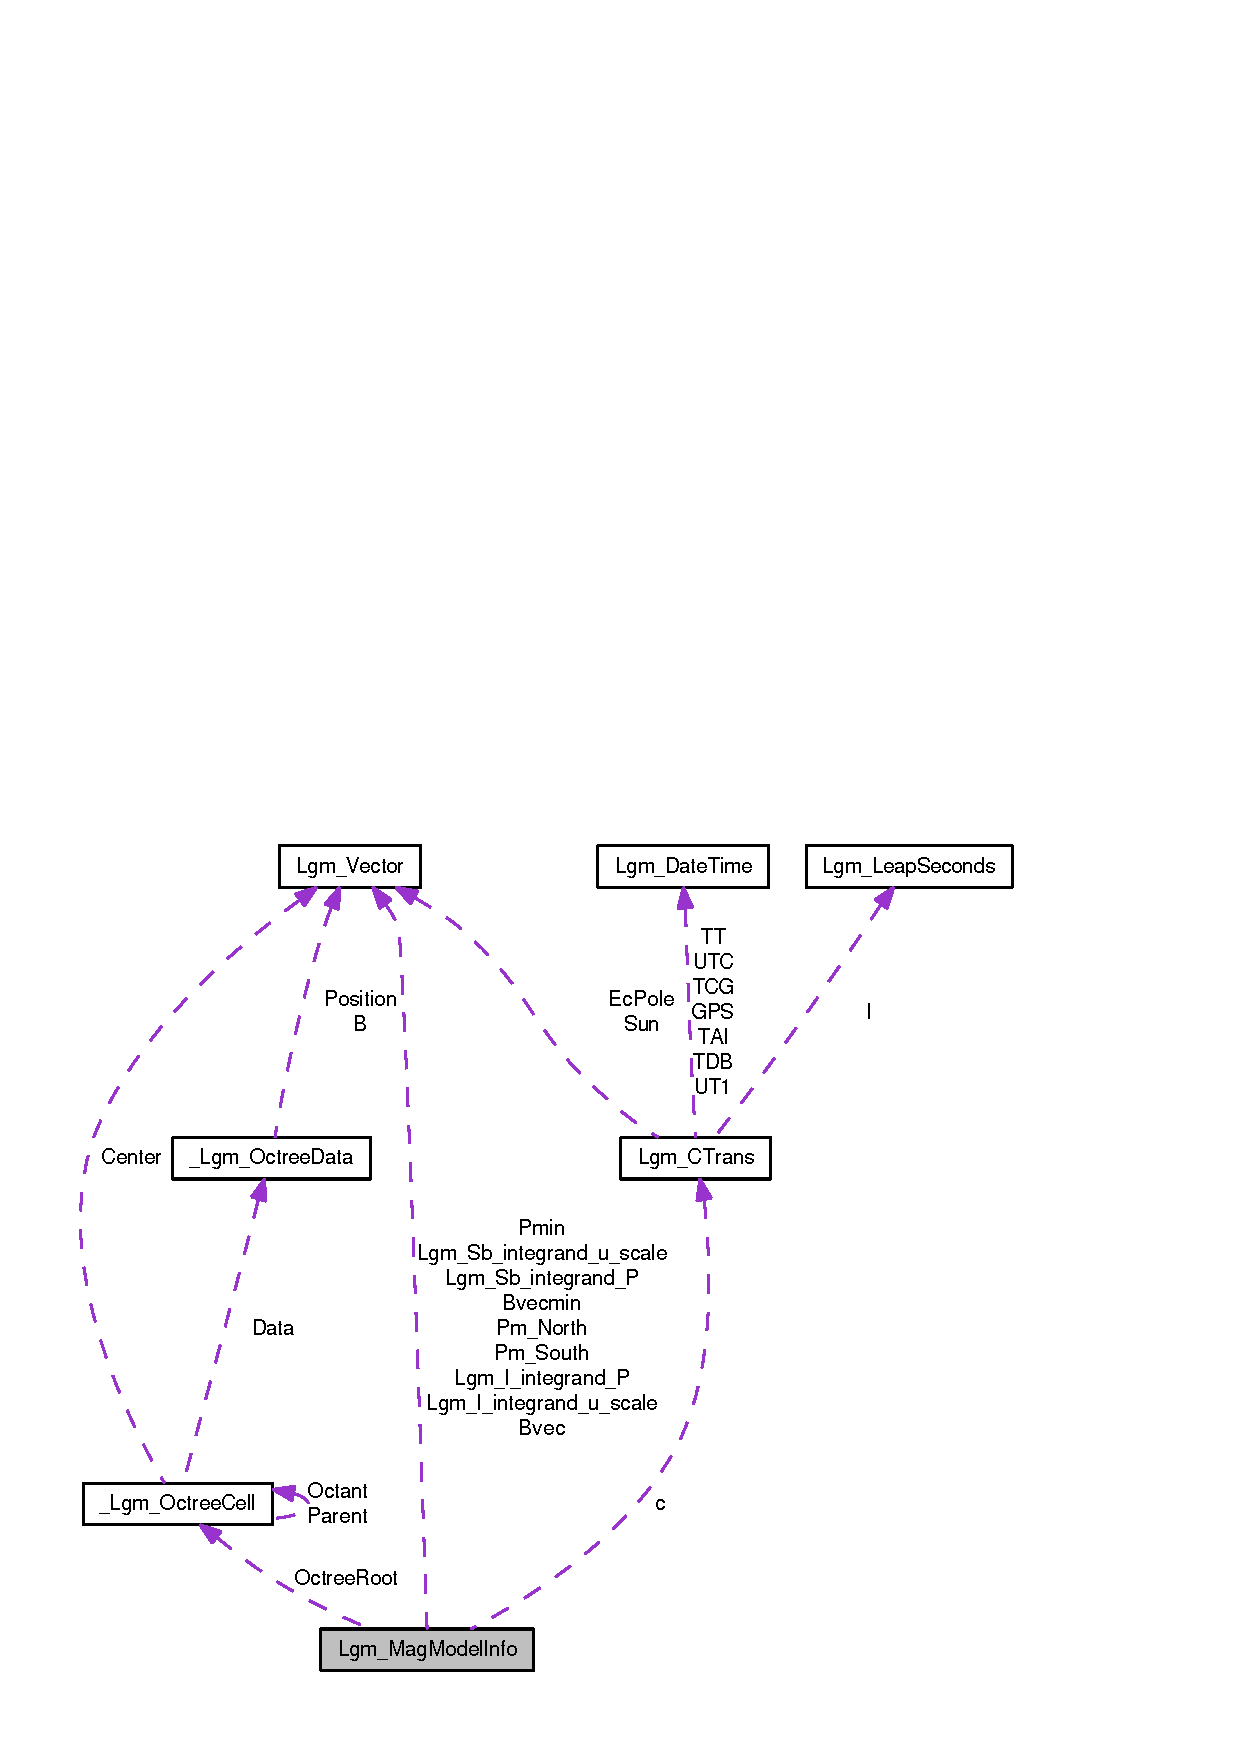
\includegraphics[width=400pt]{struct_lgm___mag_model_info__coll__graph}
\end{center}
\end{figure}
\subsection*{Data Fields}
\begin{CompactItemize}
\item 
\hyperlink{struct_lgm___c_trans}{Lgm\_\-CTrans} $\ast$ \hyperlink{struct_lgm___mag_model_info_db73b2e3eecb2b5b5d8a8d278fd592e7}{c}
\item 
long int \hyperlink{struct_lgm___mag_model_info_86d7303c776d4ec954324d5c477c79a2}{nFunc}
\item 
int($\ast$ \hyperlink{struct_lgm___mag_model_info_b0506253f98bbfee0c9a097ca2bc52fe}{Bfield} )()
\item 
int \hyperlink{struct_lgm___mag_model_info_947337af07b4114cc9f9706bfcb809de}{SavePoints}
\item 
double \hyperlink{struct_lgm___mag_model_info_d8e5a89709cc62b7538c1429c0bea670}{Hmax}
\item 
FILE $\ast$ \hyperlink{struct_lgm___mag_model_info_a065f30aa9f5f9a42132c82c787ee70b}{fp}
\item 
double \hyperlink{struct_lgm___mag_model_info_c186dbd58445ff8691db0f437f862a54}{W} \mbox{[}6\mbox{]}
\item 
int \hyperlink{struct_lgm___mag_model_info_c660713cdd5b69708fe7c4866be48b53}{Kp}
\item 
double \hyperlink{struct_lgm___mag_model_info_521a6affefa837861b71a21b021b109b}{Dst}
\item 
double \hyperlink{struct_lgm___mag_model_info_8019aa9167c19c810aefa4cd5c0b0ab5}{P}
\item 
double \hyperlink{struct_lgm___mag_model_info_5fa1384b59affe6ed504db99bba961fe}{Bx}
\item 
double \hyperlink{struct_lgm___mag_model_info_01b195b7d857f35425ee41d84eea6a1a}{By}
\item 
double \hyperlink{struct_lgm___mag_model_info_cf4e512cfc2056dc67f7f73aeb07ea3b}{Bz}
\item 
double \hyperlink{struct_lgm___mag_model_info_bc39a5f9f3bf06b9ae46dd8588d3bd79}{T96MOD\_\-V} \mbox{[}11\mbox{]}
\item 
double \hyperlink{struct_lgm___mag_model_info_d543ac40b07dbe5a76060b7f56b90094}{Trace\_\-s}
\item 
double \hyperlink{struct_lgm___mag_model_info_f8c1a0342c71ca07cc809e7e808ec81e}{B0}
\item 
double \hyperlink{struct_lgm___mag_model_info_612bfe392d6bf2d2e1a2f6e65a003f5e}{B1}
\item 
double \hyperlink{struct_lgm___mag_model_info_c25028524f0b3bb1e35a6f5b62bc4f47}{B2}
\item 
int \hyperlink{struct_lgm___mag_model_info_02a6418c4d27275421dd73a5bbb65f8c}{InternalModel}
\item 
double \hyperlink{struct_lgm___mag_model_info_869c8a1c2af0f48c6e871b08c13d2852}{KineticEnergy}
\item 
double \hyperlink{struct_lgm___mag_model_info_c33418187547ea28dda7063924f34df6}{Mass}
\item 
double \hyperlink{struct_lgm___mag_model_info_86da8321817d74036d3ff23e8643dc68}{PitchAngle}
\item 
\hyperlink{struct_lgm___vector}{Lgm\_\-Vector} \hyperlink{struct_lgm___mag_model_info_a6b4371f4272ea673b10df3806973a78}{Pm\_\-South}
\item 
\hyperlink{struct_lgm___vector}{Lgm\_\-Vector} \hyperlink{struct_lgm___mag_model_info_680815020ea7ef4edf84c04a0d7f1f20}{Pm\_\-North}
\item 
double \hyperlink{struct_lgm___mag_model_info_8e90af044e680fe06a5f4745ead8b8d7}{Bm}
\item 
double \hyperlink{struct_lgm___mag_model_info_91d445e45d4679505b1a9b5b7cde690c}{Sm\_\-South}
\item 
double \hyperlink{struct_lgm___mag_model_info_e133118dcb4b4b581ae49086e9d16be3}{Sm\_\-North}
\item 
double \hyperlink{struct_lgm___mag_model_info_3c9886361e1ccd93a330528121ebe6d3}{Blocal}
\item 
int \hyperlink{struct_lgm___mag_model_info_52587930b11ea1eb053f0306dbc7973e}{FirstCall}
\item 
double \hyperlink{struct_lgm___mag_model_info_cf41bfa63c25a6466792c68b7b483bed}{s} \mbox{[}LGM\_\-MAX\_\-INTERP\_\-PNTS\mbox{]}
\item 
double \hyperlink{struct_lgm___mag_model_info_dd03b0d5df37a9e1074dec8d2b370a2d}{Px} \mbox{[}LGM\_\-MAX\_\-INTERP\_\-PNTS\mbox{]}
\item 
double \hyperlink{struct_lgm___mag_model_info_8a91bcce4c333afd8126b6a186dd59d7}{Py} \mbox{[}LGM\_\-MAX\_\-INTERP\_\-PNTS\mbox{]}
\item 
double \hyperlink{struct_lgm___mag_model_info_042f2ba75b091726dca685c45f9be927}{Pz} \mbox{[}LGM\_\-MAX\_\-INTERP\_\-PNTS\mbox{]}
\item 
\hyperlink{struct_lgm___vector}{Lgm\_\-Vector} \hyperlink{struct_lgm___mag_model_info_ee6c1c35a439c2b6b3d968446dffb31a}{Bvec} \mbox{[}LGM\_\-MAX\_\-INTERP\_\-PNTS\mbox{]}
\item 
double \hyperlink{struct_lgm___mag_model_info_7d9e308c1b0c6e09a52f4c3c2d93b6cb}{Bmag} \mbox{[}LGM\_\-MAX\_\-INTERP\_\-PNTS\mbox{]}
\item 
double \hyperlink{struct_lgm___mag_model_info_d3f3c09afc338a28ddb1213be42a4ca7}{BminusBcdip} \mbox{[}LGM\_\-MAX\_\-INTERP\_\-PNTS\mbox{]}
\item 
int \hyperlink{struct_lgm___mag_model_info_e64e724dd0713b2ba2fca5aedab3fd34}{nPnts}
\item 
double \hyperlink{struct_lgm___mag_model_info_ac2192aa882430a630cad1a1b5131a29}{ds}
\item 
double \hyperlink{struct_lgm___mag_model_info_588dcb85c838ec933ddca7fd85319356}{smin}
\item 
double \hyperlink{struct_lgm___mag_model_info_2ac3a99381d281d4caabf024a33f0b31}{Bmin}
\item 
\hyperlink{struct_lgm___vector}{Lgm\_\-Vector} \hyperlink{struct_lgm___mag_model_info_2331552c154915274f41a4113148557b}{Bvecmin}
\item 
\hyperlink{struct_lgm___vector}{Lgm\_\-Vector} \hyperlink{struct_lgm___mag_model_info_5bafc8f6aad6cc63366225b1a7c42901}{Pmin}
\item 
double \hyperlink{struct_lgm___mag_model_info_4cfe25e04c92794254faa1a0abb4d817}{d2B\_\-ds2}
\item 
double \hyperlink{struct_lgm___mag_model_info_42a3a606a80dbe9a94436854fdef0516}{Sb0}
\item 
int \hyperlink{struct_lgm___mag_model_info_7398fdf92dfab0dfd2d5ac11eaa570bc}{imin1}
\item 
int \hyperlink{struct_lgm___mag_model_info_b38a4f405262c1ee308e925285be06c2}{imin2}
\item 
gsl\_\-interp\_\-accel $\ast$ \hyperlink{struct_lgm___mag_model_info_7c9a9e6523a7a6e67a5b349e772e3765}{acc}
\item 
gsl\_\-interp\_\-accel $\ast$ \hyperlink{struct_lgm___mag_model_info_b695ec5d60e2b6c19e995ada21303a66}{accPx}
\item 
gsl\_\-interp\_\-accel $\ast$ \hyperlink{struct_lgm___mag_model_info_debd817de2dd24802efd42e4d61248bd}{accPy}
\item 
gsl\_\-interp\_\-accel $\ast$ \hyperlink{struct_lgm___mag_model_info_3f81b52b8e022a147d3ded46c8eae116}{accPz}
\item 
gsl\_\-spline $\ast$ \hyperlink{struct_lgm___mag_model_info_a4a622517a6af76ad0ff2c6f10465fdd}{spline}
\item 
gsl\_\-spline $\ast$ \hyperlink{struct_lgm___mag_model_info_7780e74c82195c308a42a01d815e05f9}{splinePx}
\item 
gsl\_\-spline $\ast$ \hyperlink{struct_lgm___mag_model_info_1122f71b0439cefad84c3d362409af9e}{splinePy}
\item 
gsl\_\-spline $\ast$ \hyperlink{struct_lgm___mag_model_info_5463eef92d8b039ea695f0666c59c69f}{splinePz}
\item 
int \hyperlink{struct_lgm___mag_model_info_ef3011234df74566b679b46e01273bb7}{VerbosityLevel}
\item 
int \hyperlink{struct_lgm___mag_model_info_beeccfbf7295d0c631353a9159972a74}{UseInterpRoutines}
\item 
double \hyperlink{struct_lgm___mag_model_info_cbad03b970a668a0beb805a283fa01cf}{Lgm\_\-MagStep\_\-eps\_\-old}
\item 
int \hyperlink{struct_lgm___mag_model_info_fa214459195ced041bebfae2220e17c2}{Lgm\_\-MagStep\_\-FirstTimeThrough}
\item 
int \hyperlink{struct_lgm___mag_model_info_dbca9048683a6b46691f16bbc6badc91}{Lgm\_\-MagStep\_\-kmax}
\item 
int \hyperlink{struct_lgm___mag_model_info_9074ef2a6a61faf148f617fc02a8f9df}{Lgm\_\-MagStep\_\-kopt}
\item 
double \hyperlink{struct_lgm___mag_model_info_289830ee3ee42ca423ae557a9417fb90}{Lgm\_\-MagStep\_\-snew}
\item 
double \hyperlink{struct_lgm___mag_model_info_33ce6893a0952ee0bcf577a9f9f802ff}{Lgm\_\-MagStep\_\-A} \mbox{[}LGM\_\-MAGSTEP\_\-JMAX+1\mbox{]}
\item 
double \hyperlink{struct_lgm___mag_model_info_62bf5ca4d843811f15f1592223b72c79}{Lgm\_\-MagStep\_\-alpha} \mbox{[}LGM\_\-MAGSTEP\_\-IMAX+1\mbox{]}\mbox{[}LGM\_\-MAGSTEP\_\-IMAX+1\mbox{]}
\item 
double \hyperlink{struct_lgm___mag_model_info_7e69c8ba64e1329002344adc94aa6594}{Lgm\_\-MagStep\_\-d} \mbox{[}LGM\_\-MAGSTEP\_\-JMAX\mbox{]}\mbox{[}LGM\_\-MAGSTEP\_\-JMAX\mbox{]}
\item 
double \hyperlink{struct_lgm___mag_model_info_d2c62978bb8693b682121af1a5e57779}{Lgm\_\-MagStep\_\-x} \mbox{[}LGM\_\-MAGSTEP\_\-JMAX\mbox{]}
\item 
int \hyperlink{struct_lgm___mag_model_info_702cb79ba0ac9c88d1038676a4db833f}{Lgm\_\-I\_\-integrand\_\-FirstCall}
\item 
int \hyperlink{struct_lgm___mag_model_info_c3c19bdf192ad5db270e70441bfa3392}{Lgm\_\-I\_\-integrand\_\-JumpMethod}
\item 
double \hyperlink{struct_lgm___mag_model_info_bd9305e3ff7eac184a3f651ae47ae5bc}{Lgm\_\-I\_\-integrand\_\-S}
\item 
\hyperlink{struct_lgm___vector}{Lgm\_\-Vector} \hyperlink{struct_lgm___mag_model_info_a3ad9c4b833001273b79b67cb2a86d49}{Lgm\_\-I\_\-integrand\_\-P}
\item 
\hyperlink{struct_lgm___vector}{Lgm\_\-Vector} \hyperlink{struct_lgm___mag_model_info_e7d44a46b9d0110bafb9f5c47f1b047c}{Lgm\_\-I\_\-integrand\_\-u\_\-scale}
\item 
int \hyperlink{struct_lgm___mag_model_info_0b40445e52e091e26fb821e573c41ba0}{Lgm\_\-n\_\-I\_\-integrand\_\-Calls}
\item 
int \hyperlink{struct_lgm___mag_model_info_22a0997163992fbc3d980522be2fd613}{Lgm\_\-I\_\-Integrator}
\item 
double \hyperlink{struct_lgm___mag_model_info_1be8f828cb392cad59b8c27918f7862f}{Lgm\_\-I\_\-Integrator\_\-epsrel}
\item 
double \hyperlink{struct_lgm___mag_model_info_84d1542c6975c366a6b0387d6497c86b}{Lgm\_\-I\_\-Integrator\_\-epsabs}
\item 
int \hyperlink{struct_lgm___mag_model_info_53c05ef170d36948f85a32ca0f5a6912}{Lgm\_\-Sb\_\-integrand\_\-FirstCall}
\item 
double \hyperlink{struct_lgm___mag_model_info_ba782efaf640472be322e8290acac370}{Lgm\_\-Sb\_\-integrand\_\-S}
\item 
\hyperlink{struct_lgm___vector}{Lgm\_\-Vector} \hyperlink{struct_lgm___mag_model_info_64ea881b31763fe2b1c1fc78d589dd84}{Lgm\_\-Sb\_\-integrand\_\-P}
\item 
\hyperlink{struct_lgm___vector}{Lgm\_\-Vector} \hyperlink{struct_lgm___mag_model_info_fc1c449cd255aa38568f885b3732a699}{Lgm\_\-Sb\_\-integrand\_\-u\_\-scale}
\item 
int \hyperlink{struct_lgm___mag_model_info_e1edd10efda316240fd228a9bab0cc24}{Lgm\_\-n\_\-Sb\_\-integrand\_\-Calls}
\item 
int \hyperlink{struct_lgm___mag_model_info_713978104b56d5edd790199e13ee10fd}{Lgm\_\-Sb\_\-Integrator}
\item 
double \hyperlink{struct_lgm___mag_model_info_f26880c2615c83b542f39feab78bf592}{Lgm\_\-Sb\_\-Integrator\_\-epsrel}
\item 
double \hyperlink{struct_lgm___mag_model_info_128e371c7ac1d69077ca45eb79cc094e}{Lgm\_\-Sb\_\-Integrator\_\-epsabs}
\item 
int \hyperlink{struct_lgm___mag_model_info_0ba66db9846f0a3c1c41abe473719dcb}{Lgm\_\-MagFlux\_\-Integrator}
\item 
double \hyperlink{struct_lgm___mag_model_info_c15192e0cdb8a093d53b3aed95fd5899}{Lgm\_\-MagFlux\_\-Integrator\_\-epsrel}
\item 
double \hyperlink{struct_lgm___mag_model_info_2659eea0c59fae87e7ac738542e00128}{Lgm\_\-MagFlux\_\-Integrator\_\-epsabs}
\item 
int \hyperlink{struct_lgm___mag_model_info_a3ec6fe0176592c49bb9f25f9fd05a71}{Lgm\_\-LambdaIntegral\_\-Integrator}
\item 
double \hyperlink{struct_lgm___mag_model_info_c2e550303cccbc0f08c3d46975f79111}{Lgm\_\-LambdaIntegral\_\-Integrator\_\-epsrel}
\item 
double \hyperlink{struct_lgm___mag_model_info_84e45c331b0974d7470a7c5796550069}{Lgm\_\-LambdaIntegral\_\-Integrator\_\-epsabs}
\item 
double \hyperlink{struct_lgm___mag_model_info_87d9547dc23285cacd4e7eb0a4fa81c8}{Lgm\_\-FindBmRadius\_\-Tol}
\item 
double \hyperlink{struct_lgm___mag_model_info_aa3a6471b016a88d0c199e4689b5115b}{Lgm\_\-FindShellLine\_\-I\_\-Tol}
\item 
double \hyperlink{struct_lgm___mag_model_info_371678dd73a628d7a7e92195a977f2ab}{Lgm\_\-TraceToMirrorPoint\_\-Tol}
\item 
\hyperlink{struct___lgm___octree_cell}{Lgm\_\-OctreeCell} $\ast$ \hyperlink{struct_lgm___mag_model_info_3c296eee871865d5eb14f0e46f242d52}{OctreeRoot}
\item 
int \hyperlink{struct_lgm___mag_model_info_99cfcbf0b2cc678489e5610f95ba444f}{Octree\_\-kNN\_\-k}
\item 
int \hyperlink{struct_lgm___mag_model_info_5f46c646591dc34aa1dd15ae784de211}{Octree\_\-kNN\_\-InterpMethod}
\item 
double \hyperlink{struct_lgm___mag_model_info_8bb4098863c80f1488ba2210a992c1c7}{Octree\_\-kNN\_\-MaxDist}
\item 
double \hyperlink{struct_lgm___mag_model_info_010feefec439ccf0a4dbb5b3d1599e36}{OctreeScaleMin}
\item 
double \hyperlink{struct_lgm___mag_model_info_0310164485c1dbf6298b11f23531d42f}{OctreeScaleMax}
\item 
double \hyperlink{struct_lgm___mag_model_info_593eb3c7aeb022b668650a364f4a436e}{OctreeScaleDiff}
\item 
double \hyperlink{struct_lgm___mag_model_info_7d6b092f69ab45a5532b1bbc137afd0c}{OpenLimit\_\-xMin}
\item 
double \hyperlink{struct_lgm___mag_model_info_f97947f7418eed4c17c0668e8bc3cd4e}{OpenLimit\_\-xMax}
\item 
double \hyperlink{struct_lgm___mag_model_info_97e8920e1c6dd24c5cff164113bf05b3}{OpenLimit\_\-yMin}
\item 
double \hyperlink{struct_lgm___mag_model_info_abc524710dd7b86daa257d70347b2c23}{OpenLimit\_\-yMax}
\item 
double \hyperlink{struct_lgm___mag_model_info_f657d5c81e259de821321d7247c0a36d}{OpenLimit\_\-zMin}
\item 
double \hyperlink{struct_lgm___mag_model_info_8872d2067eaccc17854b021eb2db82a1}{OpenLimit\_\-zMax}
\end{CompactItemize}


\subsection{Detailed Description}


Definition at line 75 of file Lgm\_\-MagModelInfo.h.

\subsection{Field Documentation}
\hypertarget{struct_lgm___mag_model_info_db73b2e3eecb2b5b5d8a8d278fd592e7}{
\index{Lgm\_\-MagModelInfo@{Lgm\_\-MagModelInfo}!c@{c}}
\index{c@{c}!Lgm_MagModelInfo@{Lgm\_\-MagModelInfo}}
\subsubsection[{c}]{\setlength{\rightskip}{0pt plus 5cm}{\bf Lgm\_\-CTrans}$\ast$ {\bf c}}}
\label{struct_lgm___mag_model_info_db73b2e3eecb2b5b5d8a8d278fd592e7}




Definition at line 77 of file Lgm\_\-MagModelInfo.h.\hypertarget{struct_lgm___mag_model_info_86d7303c776d4ec954324d5c477c79a2}{
\index{Lgm\_\-MagModelInfo@{Lgm\_\-MagModelInfo}!nFunc@{nFunc}}
\index{nFunc@{nFunc}!Lgm_MagModelInfo@{Lgm\_\-MagModelInfo}}
\subsubsection[{nFunc}]{\setlength{\rightskip}{0pt plus 5cm}long int {\bf nFunc}}}
\label{struct_lgm___mag_model_info_86d7303c776d4ec954324d5c477c79a2}




Definition at line 78 of file Lgm\_\-MagModelInfo.h.\hypertarget{struct_lgm___mag_model_info_b0506253f98bbfee0c9a097ca2bc52fe}{
\index{Lgm\_\-MagModelInfo@{Lgm\_\-MagModelInfo}!Bfield@{Bfield}}
\index{Bfield@{Bfield}!Lgm_MagModelInfo@{Lgm\_\-MagModelInfo}}
\subsubsection[{Bfield}]{\setlength{\rightskip}{0pt plus 5cm}int($\ast$ {\bf Bfield})()}}
\label{struct_lgm___mag_model_info_b0506253f98bbfee0c9a097ca2bc52fe}


\hypertarget{struct_lgm___mag_model_info_947337af07b4114cc9f9706bfcb809de}{
\index{Lgm\_\-MagModelInfo@{Lgm\_\-MagModelInfo}!SavePoints@{SavePoints}}
\index{SavePoints@{SavePoints}!Lgm_MagModelInfo@{Lgm\_\-MagModelInfo}}
\subsubsection[{SavePoints}]{\setlength{\rightskip}{0pt plus 5cm}int {\bf SavePoints}}}
\label{struct_lgm___mag_model_info_947337af07b4114cc9f9706bfcb809de}




Definition at line 80 of file Lgm\_\-MagModelInfo.h.\hypertarget{struct_lgm___mag_model_info_d8e5a89709cc62b7538c1429c0bea670}{
\index{Lgm\_\-MagModelInfo@{Lgm\_\-MagModelInfo}!Hmax@{Hmax}}
\index{Hmax@{Hmax}!Lgm_MagModelInfo@{Lgm\_\-MagModelInfo}}
\subsubsection[{Hmax}]{\setlength{\rightskip}{0pt plus 5cm}double {\bf Hmax}}}
\label{struct_lgm___mag_model_info_d8e5a89709cc62b7538c1429c0bea670}




Definition at line 81 of file Lgm\_\-MagModelInfo.h.\hypertarget{struct_lgm___mag_model_info_a065f30aa9f5f9a42132c82c787ee70b}{
\index{Lgm\_\-MagModelInfo@{Lgm\_\-MagModelInfo}!fp@{fp}}
\index{fp@{fp}!Lgm_MagModelInfo@{Lgm\_\-MagModelInfo}}
\subsubsection[{fp}]{\setlength{\rightskip}{0pt plus 5cm}FILE$\ast$ {\bf fp}}}
\label{struct_lgm___mag_model_info_a065f30aa9f5f9a42132c82c787ee70b}




Definition at line 82 of file Lgm\_\-MagModelInfo.h.\hypertarget{struct_lgm___mag_model_info_c186dbd58445ff8691db0f437f862a54}{
\index{Lgm\_\-MagModelInfo@{Lgm\_\-MagModelInfo}!W@{W}}
\index{W@{W}!Lgm_MagModelInfo@{Lgm\_\-MagModelInfo}}
\subsubsection[{W}]{\setlength{\rightskip}{0pt plus 5cm}double {\bf W}\mbox{[}6\mbox{]}}}
\label{struct_lgm___mag_model_info_c186dbd58445ff8691db0f437f862a54}




Definition at line 83 of file Lgm\_\-MagModelInfo.h.\hypertarget{struct_lgm___mag_model_info_c660713cdd5b69708fe7c4866be48b53}{
\index{Lgm\_\-MagModelInfo@{Lgm\_\-MagModelInfo}!Kp@{Kp}}
\index{Kp@{Kp}!Lgm_MagModelInfo@{Lgm\_\-MagModelInfo}}
\subsubsection[{Kp}]{\setlength{\rightskip}{0pt plus 5cm}int {\bf Kp}}}
\label{struct_lgm___mag_model_info_c660713cdd5b69708fe7c4866be48b53}




Definition at line 84 of file Lgm\_\-MagModelInfo.h.\hypertarget{struct_lgm___mag_model_info_521a6affefa837861b71a21b021b109b}{
\index{Lgm\_\-MagModelInfo@{Lgm\_\-MagModelInfo}!Dst@{Dst}}
\index{Dst@{Dst}!Lgm_MagModelInfo@{Lgm\_\-MagModelInfo}}
\subsubsection[{Dst}]{\setlength{\rightskip}{0pt plus 5cm}double {\bf Dst}}}
\label{struct_lgm___mag_model_info_521a6affefa837861b71a21b021b109b}




Definition at line 85 of file Lgm\_\-MagModelInfo.h.\hypertarget{struct_lgm___mag_model_info_8019aa9167c19c810aefa4cd5c0b0ab5}{
\index{Lgm\_\-MagModelInfo@{Lgm\_\-MagModelInfo}!P@{P}}
\index{P@{P}!Lgm_MagModelInfo@{Lgm\_\-MagModelInfo}}
\subsubsection[{P}]{\setlength{\rightskip}{0pt plus 5cm}double {\bf P}}}
\label{struct_lgm___mag_model_info_8019aa9167c19c810aefa4cd5c0b0ab5}




Definition at line 86 of file Lgm\_\-MagModelInfo.h.\hypertarget{struct_lgm___mag_model_info_5fa1384b59affe6ed504db99bba961fe}{
\index{Lgm\_\-MagModelInfo@{Lgm\_\-MagModelInfo}!Bx@{Bx}}
\index{Bx@{Bx}!Lgm_MagModelInfo@{Lgm\_\-MagModelInfo}}
\subsubsection[{Bx}]{\setlength{\rightskip}{0pt plus 5cm}double {\bf Bx}}}
\label{struct_lgm___mag_model_info_5fa1384b59affe6ed504db99bba961fe}




Definition at line 87 of file Lgm\_\-MagModelInfo.h.\hypertarget{struct_lgm___mag_model_info_01b195b7d857f35425ee41d84eea6a1a}{
\index{Lgm\_\-MagModelInfo@{Lgm\_\-MagModelInfo}!By@{By}}
\index{By@{By}!Lgm_MagModelInfo@{Lgm\_\-MagModelInfo}}
\subsubsection[{By}]{\setlength{\rightskip}{0pt plus 5cm}double {\bf By}}}
\label{struct_lgm___mag_model_info_01b195b7d857f35425ee41d84eea6a1a}




Definition at line 87 of file Lgm\_\-MagModelInfo.h.\hypertarget{struct_lgm___mag_model_info_cf4e512cfc2056dc67f7f73aeb07ea3b}{
\index{Lgm\_\-MagModelInfo@{Lgm\_\-MagModelInfo}!Bz@{Bz}}
\index{Bz@{Bz}!Lgm_MagModelInfo@{Lgm\_\-MagModelInfo}}
\subsubsection[{Bz}]{\setlength{\rightskip}{0pt plus 5cm}double {\bf Bz}}}
\label{struct_lgm___mag_model_info_cf4e512cfc2056dc67f7f73aeb07ea3b}




Definition at line 87 of file Lgm\_\-MagModelInfo.h.\hypertarget{struct_lgm___mag_model_info_bc39a5f9f3bf06b9ae46dd8588d3bd79}{
\index{Lgm\_\-MagModelInfo@{Lgm\_\-MagModelInfo}!T96MOD\_\-V@{T96MOD\_\-V}}
\index{T96MOD\_\-V@{T96MOD\_\-V}!Lgm_MagModelInfo@{Lgm\_\-MagModelInfo}}
\subsubsection[{T96MOD\_\-V}]{\setlength{\rightskip}{0pt plus 5cm}double {\bf T96MOD\_\-V}\mbox{[}11\mbox{]}}}
\label{struct_lgm___mag_model_info_bc39a5f9f3bf06b9ae46dd8588d3bd79}




Definition at line 88 of file Lgm\_\-MagModelInfo.h.\hypertarget{struct_lgm___mag_model_info_d543ac40b07dbe5a76060b7f56b90094}{
\index{Lgm\_\-MagModelInfo@{Lgm\_\-MagModelInfo}!Trace\_\-s@{Trace\_\-s}}
\index{Trace\_\-s@{Trace\_\-s}!Lgm_MagModelInfo@{Lgm\_\-MagModelInfo}}
\subsubsection[{Trace\_\-s}]{\setlength{\rightskip}{0pt plus 5cm}double {\bf Trace\_\-s}}}
\label{struct_lgm___mag_model_info_d543ac40b07dbe5a76060b7f56b90094}




Definition at line 90 of file Lgm\_\-MagModelInfo.h.\hypertarget{struct_lgm___mag_model_info_f8c1a0342c71ca07cc809e7e808ec81e}{
\index{Lgm\_\-MagModelInfo@{Lgm\_\-MagModelInfo}!B0@{B0}}
\index{B0@{B0}!Lgm_MagModelInfo@{Lgm\_\-MagModelInfo}}
\subsubsection[{B0}]{\setlength{\rightskip}{0pt plus 5cm}double {\bf B0}}}
\label{struct_lgm___mag_model_info_f8c1a0342c71ca07cc809e7e808ec81e}




Definition at line 92 of file Lgm\_\-MagModelInfo.h.\hypertarget{struct_lgm___mag_model_info_612bfe392d6bf2d2e1a2f6e65a003f5e}{
\index{Lgm\_\-MagModelInfo@{Lgm\_\-MagModelInfo}!B1@{B1}}
\index{B1@{B1}!Lgm_MagModelInfo@{Lgm\_\-MagModelInfo}}
\subsubsection[{B1}]{\setlength{\rightskip}{0pt plus 5cm}double {\bf B1}}}
\label{struct_lgm___mag_model_info_612bfe392d6bf2d2e1a2f6e65a003f5e}




Definition at line 92 of file Lgm\_\-MagModelInfo.h.\hypertarget{struct_lgm___mag_model_info_c25028524f0b3bb1e35a6f5b62bc4f47}{
\index{Lgm\_\-MagModelInfo@{Lgm\_\-MagModelInfo}!B2@{B2}}
\index{B2@{B2}!Lgm_MagModelInfo@{Lgm\_\-MagModelInfo}}
\subsubsection[{B2}]{\setlength{\rightskip}{0pt plus 5cm}double {\bf B2}}}
\label{struct_lgm___mag_model_info_c25028524f0b3bb1e35a6f5b62bc4f47}




Definition at line 92 of file Lgm\_\-MagModelInfo.h.\hypertarget{struct_lgm___mag_model_info_02a6418c4d27275421dd73a5bbb65f8c}{
\index{Lgm\_\-MagModelInfo@{Lgm\_\-MagModelInfo}!InternalModel@{InternalModel}}
\index{InternalModel@{InternalModel}!Lgm_MagModelInfo@{Lgm\_\-MagModelInfo}}
\subsubsection[{InternalModel}]{\setlength{\rightskip}{0pt plus 5cm}int {\bf InternalModel}}}
\label{struct_lgm___mag_model_info_02a6418c4d27275421dd73a5bbb65f8c}




Definition at line 98 of file Lgm\_\-MagModelInfo.h.\hypertarget{struct_lgm___mag_model_info_869c8a1c2af0f48c6e871b08c13d2852}{
\index{Lgm\_\-MagModelInfo@{Lgm\_\-MagModelInfo}!KineticEnergy@{KineticEnergy}}
\index{KineticEnergy@{KineticEnergy}!Lgm_MagModelInfo@{Lgm\_\-MagModelInfo}}
\subsubsection[{KineticEnergy}]{\setlength{\rightskip}{0pt plus 5cm}double {\bf KineticEnergy}}}
\label{struct_lgm___mag_model_info_869c8a1c2af0f48c6e871b08c13d2852}




Definition at line 105 of file Lgm\_\-MagModelInfo.h.\hypertarget{struct_lgm___mag_model_info_c33418187547ea28dda7063924f34df6}{
\index{Lgm\_\-MagModelInfo@{Lgm\_\-MagModelInfo}!Mass@{Mass}}
\index{Mass@{Mass}!Lgm_MagModelInfo@{Lgm\_\-MagModelInfo}}
\subsubsection[{Mass}]{\setlength{\rightskip}{0pt plus 5cm}double {\bf Mass}}}
\label{struct_lgm___mag_model_info_c33418187547ea28dda7063924f34df6}




Definition at line 106 of file Lgm\_\-MagModelInfo.h.\hypertarget{struct_lgm___mag_model_info_86da8321817d74036d3ff23e8643dc68}{
\index{Lgm\_\-MagModelInfo@{Lgm\_\-MagModelInfo}!PitchAngle@{PitchAngle}}
\index{PitchAngle@{PitchAngle}!Lgm_MagModelInfo@{Lgm\_\-MagModelInfo}}
\subsubsection[{PitchAngle}]{\setlength{\rightskip}{0pt plus 5cm}double {\bf PitchAngle}}}
\label{struct_lgm___mag_model_info_86da8321817d74036d3ff23e8643dc68}




Definition at line 107 of file Lgm\_\-MagModelInfo.h.\hypertarget{struct_lgm___mag_model_info_a6b4371f4272ea673b10df3806973a78}{
\index{Lgm\_\-MagModelInfo@{Lgm\_\-MagModelInfo}!Pm\_\-South@{Pm\_\-South}}
\index{Pm\_\-South@{Pm\_\-South}!Lgm_MagModelInfo@{Lgm\_\-MagModelInfo}}
\subsubsection[{Pm\_\-South}]{\setlength{\rightskip}{0pt plus 5cm}{\bf Lgm\_\-Vector} {\bf Pm\_\-South}}}
\label{struct_lgm___mag_model_info_a6b4371f4272ea673b10df3806973a78}




Definition at line 109 of file Lgm\_\-MagModelInfo.h.\hypertarget{struct_lgm___mag_model_info_680815020ea7ef4edf84c04a0d7f1f20}{
\index{Lgm\_\-MagModelInfo@{Lgm\_\-MagModelInfo}!Pm\_\-North@{Pm\_\-North}}
\index{Pm\_\-North@{Pm\_\-North}!Lgm_MagModelInfo@{Lgm\_\-MagModelInfo}}
\subsubsection[{Pm\_\-North}]{\setlength{\rightskip}{0pt plus 5cm}{\bf Lgm\_\-Vector} {\bf Pm\_\-North}}}
\label{struct_lgm___mag_model_info_680815020ea7ef4edf84c04a0d7f1f20}




Definition at line 110 of file Lgm\_\-MagModelInfo.h.\hypertarget{struct_lgm___mag_model_info_8e90af044e680fe06a5f4745ead8b8d7}{
\index{Lgm\_\-MagModelInfo@{Lgm\_\-MagModelInfo}!Bm@{Bm}}
\index{Bm@{Bm}!Lgm_MagModelInfo@{Lgm\_\-MagModelInfo}}
\subsubsection[{Bm}]{\setlength{\rightskip}{0pt plus 5cm}double {\bf Bm}}}
\label{struct_lgm___mag_model_info_8e90af044e680fe06a5f4745ead8b8d7}




Definition at line 111 of file Lgm\_\-MagModelInfo.h.\hypertarget{struct_lgm___mag_model_info_91d445e45d4679505b1a9b5b7cde690c}{
\index{Lgm\_\-MagModelInfo@{Lgm\_\-MagModelInfo}!Sm\_\-South@{Sm\_\-South}}
\index{Sm\_\-South@{Sm\_\-South}!Lgm_MagModelInfo@{Lgm\_\-MagModelInfo}}
\subsubsection[{Sm\_\-South}]{\setlength{\rightskip}{0pt plus 5cm}double {\bf Sm\_\-South}}}
\label{struct_lgm___mag_model_info_91d445e45d4679505b1a9b5b7cde690c}




Definition at line 111 of file Lgm\_\-MagModelInfo.h.\hypertarget{struct_lgm___mag_model_info_e133118dcb4b4b581ae49086e9d16be3}{
\index{Lgm\_\-MagModelInfo@{Lgm\_\-MagModelInfo}!Sm\_\-North@{Sm\_\-North}}
\index{Sm\_\-North@{Sm\_\-North}!Lgm_MagModelInfo@{Lgm\_\-MagModelInfo}}
\subsubsection[{Sm\_\-North}]{\setlength{\rightskip}{0pt plus 5cm}double {\bf Sm\_\-North}}}
\label{struct_lgm___mag_model_info_e133118dcb4b4b581ae49086e9d16be3}




Definition at line 111 of file Lgm\_\-MagModelInfo.h.\hypertarget{struct_lgm___mag_model_info_3c9886361e1ccd93a330528121ebe6d3}{
\index{Lgm\_\-MagModelInfo@{Lgm\_\-MagModelInfo}!Blocal@{Blocal}}
\index{Blocal@{Blocal}!Lgm_MagModelInfo@{Lgm\_\-MagModelInfo}}
\subsubsection[{Blocal}]{\setlength{\rightskip}{0pt plus 5cm}double {\bf Blocal}}}
\label{struct_lgm___mag_model_info_3c9886361e1ccd93a330528121ebe6d3}




Definition at line 111 of file Lgm\_\-MagModelInfo.h.\hypertarget{struct_lgm___mag_model_info_52587930b11ea1eb053f0306dbc7973e}{
\index{Lgm\_\-MagModelInfo@{Lgm\_\-MagModelInfo}!FirstCall@{FirstCall}}
\index{FirstCall@{FirstCall}!Lgm_MagModelInfo@{Lgm\_\-MagModelInfo}}
\subsubsection[{FirstCall}]{\setlength{\rightskip}{0pt plus 5cm}int {\bf FirstCall}}}
\label{struct_lgm___mag_model_info_52587930b11ea1eb053f0306dbc7973e}




Definition at line 112 of file Lgm\_\-MagModelInfo.h.\hypertarget{struct_lgm___mag_model_info_cf41bfa63c25a6466792c68b7b483bed}{
\index{Lgm\_\-MagModelInfo@{Lgm\_\-MagModelInfo}!s@{s}}
\index{s@{s}!Lgm_MagModelInfo@{Lgm\_\-MagModelInfo}}
\subsubsection[{s}]{\setlength{\rightskip}{0pt plus 5cm}double {\bf s}\mbox{[}LGM\_\-MAX\_\-INTERP\_\-PNTS\mbox{]}}}
\label{struct_lgm___mag_model_info_cf41bfa63c25a6466792c68b7b483bed}




Definition at line 118 of file Lgm\_\-MagModelInfo.h.\hypertarget{struct_lgm___mag_model_info_dd03b0d5df37a9e1074dec8d2b370a2d}{
\index{Lgm\_\-MagModelInfo@{Lgm\_\-MagModelInfo}!Px@{Px}}
\index{Px@{Px}!Lgm_MagModelInfo@{Lgm\_\-MagModelInfo}}
\subsubsection[{Px}]{\setlength{\rightskip}{0pt plus 5cm}double {\bf Px}\mbox{[}LGM\_\-MAX\_\-INTERP\_\-PNTS\mbox{]}}}
\label{struct_lgm___mag_model_info_dd03b0d5df37a9e1074dec8d2b370a2d}




Definition at line 119 of file Lgm\_\-MagModelInfo.h.\hypertarget{struct_lgm___mag_model_info_8a91bcce4c333afd8126b6a186dd59d7}{
\index{Lgm\_\-MagModelInfo@{Lgm\_\-MagModelInfo}!Py@{Py}}
\index{Py@{Py}!Lgm_MagModelInfo@{Lgm\_\-MagModelInfo}}
\subsubsection[{Py}]{\setlength{\rightskip}{0pt plus 5cm}double {\bf Py}\mbox{[}LGM\_\-MAX\_\-INTERP\_\-PNTS\mbox{]}}}
\label{struct_lgm___mag_model_info_8a91bcce4c333afd8126b6a186dd59d7}




Definition at line 120 of file Lgm\_\-MagModelInfo.h.\hypertarget{struct_lgm___mag_model_info_042f2ba75b091726dca685c45f9be927}{
\index{Lgm\_\-MagModelInfo@{Lgm\_\-MagModelInfo}!Pz@{Pz}}
\index{Pz@{Pz}!Lgm_MagModelInfo@{Lgm\_\-MagModelInfo}}
\subsubsection[{Pz}]{\setlength{\rightskip}{0pt plus 5cm}double {\bf Pz}\mbox{[}LGM\_\-MAX\_\-INTERP\_\-PNTS\mbox{]}}}
\label{struct_lgm___mag_model_info_042f2ba75b091726dca685c45f9be927}




Definition at line 121 of file Lgm\_\-MagModelInfo.h.\hypertarget{struct_lgm___mag_model_info_ee6c1c35a439c2b6b3d968446dffb31a}{
\index{Lgm\_\-MagModelInfo@{Lgm\_\-MagModelInfo}!Bvec@{Bvec}}
\index{Bvec@{Bvec}!Lgm_MagModelInfo@{Lgm\_\-MagModelInfo}}
\subsubsection[{Bvec}]{\setlength{\rightskip}{0pt plus 5cm}{\bf Lgm\_\-Vector} {\bf Bvec}\mbox{[}LGM\_\-MAX\_\-INTERP\_\-PNTS\mbox{]}}}
\label{struct_lgm___mag_model_info_ee6c1c35a439c2b6b3d968446dffb31a}




Definition at line 122 of file Lgm\_\-MagModelInfo.h.\hypertarget{struct_lgm___mag_model_info_7d9e308c1b0c6e09a52f4c3c2d93b6cb}{
\index{Lgm\_\-MagModelInfo@{Lgm\_\-MagModelInfo}!Bmag@{Bmag}}
\index{Bmag@{Bmag}!Lgm_MagModelInfo@{Lgm\_\-MagModelInfo}}
\subsubsection[{Bmag}]{\setlength{\rightskip}{0pt plus 5cm}double {\bf Bmag}\mbox{[}LGM\_\-MAX\_\-INTERP\_\-PNTS\mbox{]}}}
\label{struct_lgm___mag_model_info_7d9e308c1b0c6e09a52f4c3c2d93b6cb}




Definition at line 123 of file Lgm\_\-MagModelInfo.h.\hypertarget{struct_lgm___mag_model_info_d3f3c09afc338a28ddb1213be42a4ca7}{
\index{Lgm\_\-MagModelInfo@{Lgm\_\-MagModelInfo}!BminusBcdip@{BminusBcdip}}
\index{BminusBcdip@{BminusBcdip}!Lgm_MagModelInfo@{Lgm\_\-MagModelInfo}}
\subsubsection[{BminusBcdip}]{\setlength{\rightskip}{0pt plus 5cm}double {\bf BminusBcdip}\mbox{[}LGM\_\-MAX\_\-INTERP\_\-PNTS\mbox{]}}}
\label{struct_lgm___mag_model_info_d3f3c09afc338a28ddb1213be42a4ca7}




Definition at line 124 of file Lgm\_\-MagModelInfo.h.\hypertarget{struct_lgm___mag_model_info_e64e724dd0713b2ba2fca5aedab3fd34}{
\index{Lgm\_\-MagModelInfo@{Lgm\_\-MagModelInfo}!nPnts@{nPnts}}
\index{nPnts@{nPnts}!Lgm_MagModelInfo@{Lgm\_\-MagModelInfo}}
\subsubsection[{nPnts}]{\setlength{\rightskip}{0pt plus 5cm}int {\bf nPnts}}}
\label{struct_lgm___mag_model_info_e64e724dd0713b2ba2fca5aedab3fd34}




Definition at line 125 of file Lgm\_\-MagModelInfo.h.\hypertarget{struct_lgm___mag_model_info_ac2192aa882430a630cad1a1b5131a29}{
\index{Lgm\_\-MagModelInfo@{Lgm\_\-MagModelInfo}!ds@{ds}}
\index{ds@{ds}!Lgm_MagModelInfo@{Lgm\_\-MagModelInfo}}
\subsubsection[{ds}]{\setlength{\rightskip}{0pt plus 5cm}double {\bf ds}}}
\label{struct_lgm___mag_model_info_ac2192aa882430a630cad1a1b5131a29}




Definition at line 126 of file Lgm\_\-MagModelInfo.h.\hypertarget{struct_lgm___mag_model_info_588dcb85c838ec933ddca7fd85319356}{
\index{Lgm\_\-MagModelInfo@{Lgm\_\-MagModelInfo}!smin@{smin}}
\index{smin@{smin}!Lgm_MagModelInfo@{Lgm\_\-MagModelInfo}}
\subsubsection[{smin}]{\setlength{\rightskip}{0pt plus 5cm}double {\bf smin}}}
\label{struct_lgm___mag_model_info_588dcb85c838ec933ddca7fd85319356}




Definition at line 129 of file Lgm\_\-MagModelInfo.h.\hypertarget{struct_lgm___mag_model_info_2ac3a99381d281d4caabf024a33f0b31}{
\index{Lgm\_\-MagModelInfo@{Lgm\_\-MagModelInfo}!Bmin@{Bmin}}
\index{Bmin@{Bmin}!Lgm_MagModelInfo@{Lgm\_\-MagModelInfo}}
\subsubsection[{Bmin}]{\setlength{\rightskip}{0pt plus 5cm}double {\bf Bmin}}}
\label{struct_lgm___mag_model_info_2ac3a99381d281d4caabf024a33f0b31}




Definition at line 130 of file Lgm\_\-MagModelInfo.h.\hypertarget{struct_lgm___mag_model_info_2331552c154915274f41a4113148557b}{
\index{Lgm\_\-MagModelInfo@{Lgm\_\-MagModelInfo}!Bvecmin@{Bvecmin}}
\index{Bvecmin@{Bvecmin}!Lgm_MagModelInfo@{Lgm\_\-MagModelInfo}}
\subsubsection[{Bvecmin}]{\setlength{\rightskip}{0pt plus 5cm}{\bf Lgm\_\-Vector} {\bf Bvecmin}}}
\label{struct_lgm___mag_model_info_2331552c154915274f41a4113148557b}




Definition at line 131 of file Lgm\_\-MagModelInfo.h.\hypertarget{struct_lgm___mag_model_info_5bafc8f6aad6cc63366225b1a7c42901}{
\index{Lgm\_\-MagModelInfo@{Lgm\_\-MagModelInfo}!Pmin@{Pmin}}
\index{Pmin@{Pmin}!Lgm_MagModelInfo@{Lgm\_\-MagModelInfo}}
\subsubsection[{Pmin}]{\setlength{\rightskip}{0pt plus 5cm}{\bf Lgm\_\-Vector} {\bf Pmin}}}
\label{struct_lgm___mag_model_info_5bafc8f6aad6cc63366225b1a7c42901}




Definition at line 132 of file Lgm\_\-MagModelInfo.h.\hypertarget{struct_lgm___mag_model_info_4cfe25e04c92794254faa1a0abb4d817}{
\index{Lgm\_\-MagModelInfo@{Lgm\_\-MagModelInfo}!d2B\_\-ds2@{d2B\_\-ds2}}
\index{d2B\_\-ds2@{d2B\_\-ds2}!Lgm_MagModelInfo@{Lgm\_\-MagModelInfo}}
\subsubsection[{d2B\_\-ds2}]{\setlength{\rightskip}{0pt plus 5cm}double {\bf d2B\_\-ds2}}}
\label{struct_lgm___mag_model_info_4cfe25e04c92794254faa1a0abb4d817}




Definition at line 133 of file Lgm\_\-MagModelInfo.h.\hypertarget{struct_lgm___mag_model_info_42a3a606a80dbe9a94436854fdef0516}{
\index{Lgm\_\-MagModelInfo@{Lgm\_\-MagModelInfo}!Sb0@{Sb0}}
\index{Sb0@{Sb0}!Lgm_MagModelInfo@{Lgm\_\-MagModelInfo}}
\subsubsection[{Sb0}]{\setlength{\rightskip}{0pt plus 5cm}double {\bf Sb0}}}
\label{struct_lgm___mag_model_info_42a3a606a80dbe9a94436854fdef0516}




Definition at line 134 of file Lgm\_\-MagModelInfo.h.\hypertarget{struct_lgm___mag_model_info_7398fdf92dfab0dfd2d5ac11eaa570bc}{
\index{Lgm\_\-MagModelInfo@{Lgm\_\-MagModelInfo}!imin1@{imin1}}
\index{imin1@{imin1}!Lgm_MagModelInfo@{Lgm\_\-MagModelInfo}}
\subsubsection[{imin1}]{\setlength{\rightskip}{0pt plus 5cm}int {\bf imin1}}}
\label{struct_lgm___mag_model_info_7398fdf92dfab0dfd2d5ac11eaa570bc}




Definition at line 135 of file Lgm\_\-MagModelInfo.h.\hypertarget{struct_lgm___mag_model_info_b38a4f405262c1ee308e925285be06c2}{
\index{Lgm\_\-MagModelInfo@{Lgm\_\-MagModelInfo}!imin2@{imin2}}
\index{imin2@{imin2}!Lgm_MagModelInfo@{Lgm\_\-MagModelInfo}}
\subsubsection[{imin2}]{\setlength{\rightskip}{0pt plus 5cm}int {\bf imin2}}}
\label{struct_lgm___mag_model_info_b38a4f405262c1ee308e925285be06c2}




Definition at line 136 of file Lgm\_\-MagModelInfo.h.\hypertarget{struct_lgm___mag_model_info_7c9a9e6523a7a6e67a5b349e772e3765}{
\index{Lgm\_\-MagModelInfo@{Lgm\_\-MagModelInfo}!acc@{acc}}
\index{acc@{acc}!Lgm_MagModelInfo@{Lgm\_\-MagModelInfo}}
\subsubsection[{acc}]{\setlength{\rightskip}{0pt plus 5cm}gsl\_\-interp\_\-accel$\ast$ {\bf acc}}}
\label{struct_lgm___mag_model_info_7c9a9e6523a7a6e67a5b349e772e3765}




Definition at line 141 of file Lgm\_\-MagModelInfo.h.\hypertarget{struct_lgm___mag_model_info_b695ec5d60e2b6c19e995ada21303a66}{
\index{Lgm\_\-MagModelInfo@{Lgm\_\-MagModelInfo}!accPx@{accPx}}
\index{accPx@{accPx}!Lgm_MagModelInfo@{Lgm\_\-MagModelInfo}}
\subsubsection[{accPx}]{\setlength{\rightskip}{0pt plus 5cm}gsl\_\-interp\_\-accel$\ast$ {\bf accPx}}}
\label{struct_lgm___mag_model_info_b695ec5d60e2b6c19e995ada21303a66}




Definition at line 142 of file Lgm\_\-MagModelInfo.h.\hypertarget{struct_lgm___mag_model_info_debd817de2dd24802efd42e4d61248bd}{
\index{Lgm\_\-MagModelInfo@{Lgm\_\-MagModelInfo}!accPy@{accPy}}
\index{accPy@{accPy}!Lgm_MagModelInfo@{Lgm\_\-MagModelInfo}}
\subsubsection[{accPy}]{\setlength{\rightskip}{0pt plus 5cm}gsl\_\-interp\_\-accel$\ast$ {\bf accPy}}}
\label{struct_lgm___mag_model_info_debd817de2dd24802efd42e4d61248bd}




Definition at line 143 of file Lgm\_\-MagModelInfo.h.\hypertarget{struct_lgm___mag_model_info_3f81b52b8e022a147d3ded46c8eae116}{
\index{Lgm\_\-MagModelInfo@{Lgm\_\-MagModelInfo}!accPz@{accPz}}
\index{accPz@{accPz}!Lgm_MagModelInfo@{Lgm\_\-MagModelInfo}}
\subsubsection[{accPz}]{\setlength{\rightskip}{0pt plus 5cm}gsl\_\-interp\_\-accel$\ast$ {\bf accPz}}}
\label{struct_lgm___mag_model_info_3f81b52b8e022a147d3ded46c8eae116}




Definition at line 144 of file Lgm\_\-MagModelInfo.h.\hypertarget{struct_lgm___mag_model_info_a4a622517a6af76ad0ff2c6f10465fdd}{
\index{Lgm\_\-MagModelInfo@{Lgm\_\-MagModelInfo}!spline@{spline}}
\index{spline@{spline}!Lgm_MagModelInfo@{Lgm\_\-MagModelInfo}}
\subsubsection[{spline}]{\setlength{\rightskip}{0pt plus 5cm}gsl\_\-spline$\ast$ {\bf spline}}}
\label{struct_lgm___mag_model_info_a4a622517a6af76ad0ff2c6f10465fdd}




Definition at line 145 of file Lgm\_\-MagModelInfo.h.\hypertarget{struct_lgm___mag_model_info_7780e74c82195c308a42a01d815e05f9}{
\index{Lgm\_\-MagModelInfo@{Lgm\_\-MagModelInfo}!splinePx@{splinePx}}
\index{splinePx@{splinePx}!Lgm_MagModelInfo@{Lgm\_\-MagModelInfo}}
\subsubsection[{splinePx}]{\setlength{\rightskip}{0pt plus 5cm}gsl\_\-spline$\ast$ {\bf splinePx}}}
\label{struct_lgm___mag_model_info_7780e74c82195c308a42a01d815e05f9}




Definition at line 146 of file Lgm\_\-MagModelInfo.h.\hypertarget{struct_lgm___mag_model_info_1122f71b0439cefad84c3d362409af9e}{
\index{Lgm\_\-MagModelInfo@{Lgm\_\-MagModelInfo}!splinePy@{splinePy}}
\index{splinePy@{splinePy}!Lgm_MagModelInfo@{Lgm\_\-MagModelInfo}}
\subsubsection[{splinePy}]{\setlength{\rightskip}{0pt plus 5cm}gsl\_\-spline$\ast$ {\bf splinePy}}}
\label{struct_lgm___mag_model_info_1122f71b0439cefad84c3d362409af9e}




Definition at line 147 of file Lgm\_\-MagModelInfo.h.\hypertarget{struct_lgm___mag_model_info_5463eef92d8b039ea695f0666c59c69f}{
\index{Lgm\_\-MagModelInfo@{Lgm\_\-MagModelInfo}!splinePz@{splinePz}}
\index{splinePz@{splinePz}!Lgm_MagModelInfo@{Lgm\_\-MagModelInfo}}
\subsubsection[{splinePz}]{\setlength{\rightskip}{0pt plus 5cm}gsl\_\-spline$\ast$ {\bf splinePz}}}
\label{struct_lgm___mag_model_info_5463eef92d8b039ea695f0666c59c69f}




Definition at line 148 of file Lgm\_\-MagModelInfo.h.\hypertarget{struct_lgm___mag_model_info_ef3011234df74566b679b46e01273bb7}{
\index{Lgm\_\-MagModelInfo@{Lgm\_\-MagModelInfo}!VerbosityLevel@{VerbosityLevel}}
\index{VerbosityLevel@{VerbosityLevel}!Lgm_MagModelInfo@{Lgm\_\-MagModelInfo}}
\subsubsection[{VerbosityLevel}]{\setlength{\rightskip}{0pt plus 5cm}int {\bf VerbosityLevel}}}
\label{struct_lgm___mag_model_info_ef3011234df74566b679b46e01273bb7}




Definition at line 155 of file Lgm\_\-MagModelInfo.h.\hypertarget{struct_lgm___mag_model_info_beeccfbf7295d0c631353a9159972a74}{
\index{Lgm\_\-MagModelInfo@{Lgm\_\-MagModelInfo}!UseInterpRoutines@{UseInterpRoutines}}
\index{UseInterpRoutines@{UseInterpRoutines}!Lgm_MagModelInfo@{Lgm\_\-MagModelInfo}}
\subsubsection[{UseInterpRoutines}]{\setlength{\rightskip}{0pt plus 5cm}int {\bf UseInterpRoutines}}}
\label{struct_lgm___mag_model_info_beeccfbf7295d0c631353a9159972a74}




Definition at line 156 of file Lgm\_\-MagModelInfo.h.\hypertarget{struct_lgm___mag_model_info_cbad03b970a668a0beb805a283fa01cf}{
\index{Lgm\_\-MagModelInfo@{Lgm\_\-MagModelInfo}!Lgm\_\-MagStep\_\-eps\_\-old@{Lgm\_\-MagStep\_\-eps\_\-old}}
\index{Lgm\_\-MagStep\_\-eps\_\-old@{Lgm\_\-MagStep\_\-eps\_\-old}!Lgm_MagModelInfo@{Lgm\_\-MagModelInfo}}
\subsubsection[{Lgm\_\-MagStep\_\-eps\_\-old}]{\setlength{\rightskip}{0pt plus 5cm}double {\bf Lgm\_\-MagStep\_\-eps\_\-old}}}
\label{struct_lgm___mag_model_info_cbad03b970a668a0beb805a283fa01cf}




Definition at line 163 of file Lgm\_\-MagModelInfo.h.\hypertarget{struct_lgm___mag_model_info_fa214459195ced041bebfae2220e17c2}{
\index{Lgm\_\-MagModelInfo@{Lgm\_\-MagModelInfo}!Lgm\_\-MagStep\_\-FirstTimeThrough@{Lgm\_\-MagStep\_\-FirstTimeThrough}}
\index{Lgm\_\-MagStep\_\-FirstTimeThrough@{Lgm\_\-MagStep\_\-FirstTimeThrough}!Lgm_MagModelInfo@{Lgm\_\-MagModelInfo}}
\subsubsection[{Lgm\_\-MagStep\_\-FirstTimeThrough}]{\setlength{\rightskip}{0pt plus 5cm}int {\bf Lgm\_\-MagStep\_\-FirstTimeThrough}}}
\label{struct_lgm___mag_model_info_fa214459195ced041bebfae2220e17c2}




Definition at line 164 of file Lgm\_\-MagModelInfo.h.\hypertarget{struct_lgm___mag_model_info_dbca9048683a6b46691f16bbc6badc91}{
\index{Lgm\_\-MagModelInfo@{Lgm\_\-MagModelInfo}!Lgm\_\-MagStep\_\-kmax@{Lgm\_\-MagStep\_\-kmax}}
\index{Lgm\_\-MagStep\_\-kmax@{Lgm\_\-MagStep\_\-kmax}!Lgm_MagModelInfo@{Lgm\_\-MagModelInfo}}
\subsubsection[{Lgm\_\-MagStep\_\-kmax}]{\setlength{\rightskip}{0pt plus 5cm}int {\bf Lgm\_\-MagStep\_\-kmax}}}
\label{struct_lgm___mag_model_info_dbca9048683a6b46691f16bbc6badc91}




Definition at line 165 of file Lgm\_\-MagModelInfo.h.\hypertarget{struct_lgm___mag_model_info_9074ef2a6a61faf148f617fc02a8f9df}{
\index{Lgm\_\-MagModelInfo@{Lgm\_\-MagModelInfo}!Lgm\_\-MagStep\_\-kopt@{Lgm\_\-MagStep\_\-kopt}}
\index{Lgm\_\-MagStep\_\-kopt@{Lgm\_\-MagStep\_\-kopt}!Lgm_MagModelInfo@{Lgm\_\-MagModelInfo}}
\subsubsection[{Lgm\_\-MagStep\_\-kopt}]{\setlength{\rightskip}{0pt plus 5cm}int {\bf Lgm\_\-MagStep\_\-kopt}}}
\label{struct_lgm___mag_model_info_9074ef2a6a61faf148f617fc02a8f9df}




Definition at line 166 of file Lgm\_\-MagModelInfo.h.\hypertarget{struct_lgm___mag_model_info_289830ee3ee42ca423ae557a9417fb90}{
\index{Lgm\_\-MagModelInfo@{Lgm\_\-MagModelInfo}!Lgm\_\-MagStep\_\-snew@{Lgm\_\-MagStep\_\-snew}}
\index{Lgm\_\-MagStep\_\-snew@{Lgm\_\-MagStep\_\-snew}!Lgm_MagModelInfo@{Lgm\_\-MagModelInfo}}
\subsubsection[{Lgm\_\-MagStep\_\-snew}]{\setlength{\rightskip}{0pt plus 5cm}double {\bf Lgm\_\-MagStep\_\-snew}}}
\label{struct_lgm___mag_model_info_289830ee3ee42ca423ae557a9417fb90}




Definition at line 167 of file Lgm\_\-MagModelInfo.h.\hypertarget{struct_lgm___mag_model_info_33ce6893a0952ee0bcf577a9f9f802ff}{
\index{Lgm\_\-MagModelInfo@{Lgm\_\-MagModelInfo}!Lgm\_\-MagStep\_\-A@{Lgm\_\-MagStep\_\-A}}
\index{Lgm\_\-MagStep\_\-A@{Lgm\_\-MagStep\_\-A}!Lgm_MagModelInfo@{Lgm\_\-MagModelInfo}}
\subsubsection[{Lgm\_\-MagStep\_\-A}]{\setlength{\rightskip}{0pt plus 5cm}double {\bf Lgm\_\-MagStep\_\-A}\mbox{[}LGM\_\-MAGSTEP\_\-JMAX+1\mbox{]}}}
\label{struct_lgm___mag_model_info_33ce6893a0952ee0bcf577a9f9f802ff}




Definition at line 168 of file Lgm\_\-MagModelInfo.h.\hypertarget{struct_lgm___mag_model_info_62bf5ca4d843811f15f1592223b72c79}{
\index{Lgm\_\-MagModelInfo@{Lgm\_\-MagModelInfo}!Lgm\_\-MagStep\_\-alpha@{Lgm\_\-MagStep\_\-alpha}}
\index{Lgm\_\-MagStep\_\-alpha@{Lgm\_\-MagStep\_\-alpha}!Lgm_MagModelInfo@{Lgm\_\-MagModelInfo}}
\subsubsection[{Lgm\_\-MagStep\_\-alpha}]{\setlength{\rightskip}{0pt plus 5cm}double {\bf Lgm\_\-MagStep\_\-alpha}\mbox{[}LGM\_\-MAGSTEP\_\-IMAX+1\mbox{]}\mbox{[}LGM\_\-MAGSTEP\_\-IMAX+1\mbox{]}}}
\label{struct_lgm___mag_model_info_62bf5ca4d843811f15f1592223b72c79}




Definition at line 169 of file Lgm\_\-MagModelInfo.h.\hypertarget{struct_lgm___mag_model_info_7e69c8ba64e1329002344adc94aa6594}{
\index{Lgm\_\-MagModelInfo@{Lgm\_\-MagModelInfo}!Lgm\_\-MagStep\_\-d@{Lgm\_\-MagStep\_\-d}}
\index{Lgm\_\-MagStep\_\-d@{Lgm\_\-MagStep\_\-d}!Lgm_MagModelInfo@{Lgm\_\-MagModelInfo}}
\subsubsection[{Lgm\_\-MagStep\_\-d}]{\setlength{\rightskip}{0pt plus 5cm}double {\bf Lgm\_\-MagStep\_\-d}\mbox{[}LGM\_\-MAGSTEP\_\-JMAX\mbox{]}\mbox{[}LGM\_\-MAGSTEP\_\-JMAX\mbox{]}}}
\label{struct_lgm___mag_model_info_7e69c8ba64e1329002344adc94aa6594}




Definition at line 170 of file Lgm\_\-MagModelInfo.h.\hypertarget{struct_lgm___mag_model_info_d2c62978bb8693b682121af1a5e57779}{
\index{Lgm\_\-MagModelInfo@{Lgm\_\-MagModelInfo}!Lgm\_\-MagStep\_\-x@{Lgm\_\-MagStep\_\-x}}
\index{Lgm\_\-MagStep\_\-x@{Lgm\_\-MagStep\_\-x}!Lgm_MagModelInfo@{Lgm\_\-MagModelInfo}}
\subsubsection[{Lgm\_\-MagStep\_\-x}]{\setlength{\rightskip}{0pt plus 5cm}double {\bf Lgm\_\-MagStep\_\-x}\mbox{[}LGM\_\-MAGSTEP\_\-JMAX\mbox{]}}}
\label{struct_lgm___mag_model_info_d2c62978bb8693b682121af1a5e57779}




Definition at line 171 of file Lgm\_\-MagModelInfo.h.\hypertarget{struct_lgm___mag_model_info_702cb79ba0ac9c88d1038676a4db833f}{
\index{Lgm\_\-MagModelInfo@{Lgm\_\-MagModelInfo}!Lgm\_\-I\_\-integrand\_\-FirstCall@{Lgm\_\-I\_\-integrand\_\-FirstCall}}
\index{Lgm\_\-I\_\-integrand\_\-FirstCall@{Lgm\_\-I\_\-integrand\_\-FirstCall}!Lgm_MagModelInfo@{Lgm\_\-MagModelInfo}}
\subsubsection[{Lgm\_\-I\_\-integrand\_\-FirstCall}]{\setlength{\rightskip}{0pt plus 5cm}int {\bf Lgm\_\-I\_\-integrand\_\-FirstCall}}}
\label{struct_lgm___mag_model_info_702cb79ba0ac9c88d1038676a4db833f}




Definition at line 178 of file Lgm\_\-MagModelInfo.h.\hypertarget{struct_lgm___mag_model_info_c3c19bdf192ad5db270e70441bfa3392}{
\index{Lgm\_\-MagModelInfo@{Lgm\_\-MagModelInfo}!Lgm\_\-I\_\-integrand\_\-JumpMethod@{Lgm\_\-I\_\-integrand\_\-JumpMethod}}
\index{Lgm\_\-I\_\-integrand\_\-JumpMethod@{Lgm\_\-I\_\-integrand\_\-JumpMethod}!Lgm_MagModelInfo@{Lgm\_\-MagModelInfo}}
\subsubsection[{Lgm\_\-I\_\-integrand\_\-JumpMethod}]{\setlength{\rightskip}{0pt plus 5cm}int {\bf Lgm\_\-I\_\-integrand\_\-JumpMethod}}}
\label{struct_lgm___mag_model_info_c3c19bdf192ad5db270e70441bfa3392}




Definition at line 179 of file Lgm\_\-MagModelInfo.h.\hypertarget{struct_lgm___mag_model_info_bd9305e3ff7eac184a3f651ae47ae5bc}{
\index{Lgm\_\-MagModelInfo@{Lgm\_\-MagModelInfo}!Lgm\_\-I\_\-integrand\_\-S@{Lgm\_\-I\_\-integrand\_\-S}}
\index{Lgm\_\-I\_\-integrand\_\-S@{Lgm\_\-I\_\-integrand\_\-S}!Lgm_MagModelInfo@{Lgm\_\-MagModelInfo}}
\subsubsection[{Lgm\_\-I\_\-integrand\_\-S}]{\setlength{\rightskip}{0pt plus 5cm}double {\bf Lgm\_\-I\_\-integrand\_\-S}}}
\label{struct_lgm___mag_model_info_bd9305e3ff7eac184a3f651ae47ae5bc}




Definition at line 180 of file Lgm\_\-MagModelInfo.h.\hypertarget{struct_lgm___mag_model_info_a3ad9c4b833001273b79b67cb2a86d49}{
\index{Lgm\_\-MagModelInfo@{Lgm\_\-MagModelInfo}!Lgm\_\-I\_\-integrand\_\-P@{Lgm\_\-I\_\-integrand\_\-P}}
\index{Lgm\_\-I\_\-integrand\_\-P@{Lgm\_\-I\_\-integrand\_\-P}!Lgm_MagModelInfo@{Lgm\_\-MagModelInfo}}
\subsubsection[{Lgm\_\-I\_\-integrand\_\-P}]{\setlength{\rightskip}{0pt plus 5cm}{\bf Lgm\_\-Vector} {\bf Lgm\_\-I\_\-integrand\_\-P}}}
\label{struct_lgm___mag_model_info_a3ad9c4b833001273b79b67cb2a86d49}




Definition at line 181 of file Lgm\_\-MagModelInfo.h.\hypertarget{struct_lgm___mag_model_info_e7d44a46b9d0110bafb9f5c47f1b047c}{
\index{Lgm\_\-MagModelInfo@{Lgm\_\-MagModelInfo}!Lgm\_\-I\_\-integrand\_\-u\_\-scale@{Lgm\_\-I\_\-integrand\_\-u\_\-scale}}
\index{Lgm\_\-I\_\-integrand\_\-u\_\-scale@{Lgm\_\-I\_\-integrand\_\-u\_\-scale}!Lgm_MagModelInfo@{Lgm\_\-MagModelInfo}}
\subsubsection[{Lgm\_\-I\_\-integrand\_\-u\_\-scale}]{\setlength{\rightskip}{0pt plus 5cm}{\bf Lgm\_\-Vector} {\bf Lgm\_\-I\_\-integrand\_\-u\_\-scale}}}
\label{struct_lgm___mag_model_info_e7d44a46b9d0110bafb9f5c47f1b047c}




Definition at line 182 of file Lgm\_\-MagModelInfo.h.\hypertarget{struct_lgm___mag_model_info_0b40445e52e091e26fb821e573c41ba0}{
\index{Lgm\_\-MagModelInfo@{Lgm\_\-MagModelInfo}!Lgm\_\-n\_\-I\_\-integrand\_\-Calls@{Lgm\_\-n\_\-I\_\-integrand\_\-Calls}}
\index{Lgm\_\-n\_\-I\_\-integrand\_\-Calls@{Lgm\_\-n\_\-I\_\-integrand\_\-Calls}!Lgm_MagModelInfo@{Lgm\_\-MagModelInfo}}
\subsubsection[{Lgm\_\-n\_\-I\_\-integrand\_\-Calls}]{\setlength{\rightskip}{0pt plus 5cm}int {\bf Lgm\_\-n\_\-I\_\-integrand\_\-Calls}}}
\label{struct_lgm___mag_model_info_0b40445e52e091e26fb821e573c41ba0}




Definition at line 183 of file Lgm\_\-MagModelInfo.h.\hypertarget{struct_lgm___mag_model_info_22a0997163992fbc3d980522be2fd613}{
\index{Lgm\_\-MagModelInfo@{Lgm\_\-MagModelInfo}!Lgm\_\-I\_\-Integrator@{Lgm\_\-I\_\-Integrator}}
\index{Lgm\_\-I\_\-Integrator@{Lgm\_\-I\_\-Integrator}!Lgm_MagModelInfo@{Lgm\_\-MagModelInfo}}
\subsubsection[{Lgm\_\-I\_\-Integrator}]{\setlength{\rightskip}{0pt plus 5cm}int {\bf Lgm\_\-I\_\-Integrator}}}
\label{struct_lgm___mag_model_info_22a0997163992fbc3d980522be2fd613}




Definition at line 184 of file Lgm\_\-MagModelInfo.h.\hypertarget{struct_lgm___mag_model_info_1be8f828cb392cad59b8c27918f7862f}{
\index{Lgm\_\-MagModelInfo@{Lgm\_\-MagModelInfo}!Lgm\_\-I\_\-Integrator\_\-epsrel@{Lgm\_\-I\_\-Integrator\_\-epsrel}}
\index{Lgm\_\-I\_\-Integrator\_\-epsrel@{Lgm\_\-I\_\-Integrator\_\-epsrel}!Lgm_MagModelInfo@{Lgm\_\-MagModelInfo}}
\subsubsection[{Lgm\_\-I\_\-Integrator\_\-epsrel}]{\setlength{\rightskip}{0pt plus 5cm}double {\bf Lgm\_\-I\_\-Integrator\_\-epsrel}}}
\label{struct_lgm___mag_model_info_1be8f828cb392cad59b8c27918f7862f}




Definition at line 185 of file Lgm\_\-MagModelInfo.h.\hypertarget{struct_lgm___mag_model_info_84d1542c6975c366a6b0387d6497c86b}{
\index{Lgm\_\-MagModelInfo@{Lgm\_\-MagModelInfo}!Lgm\_\-I\_\-Integrator\_\-epsabs@{Lgm\_\-I\_\-Integrator\_\-epsabs}}
\index{Lgm\_\-I\_\-Integrator\_\-epsabs@{Lgm\_\-I\_\-Integrator\_\-epsabs}!Lgm_MagModelInfo@{Lgm\_\-MagModelInfo}}
\subsubsection[{Lgm\_\-I\_\-Integrator\_\-epsabs}]{\setlength{\rightskip}{0pt plus 5cm}double {\bf Lgm\_\-I\_\-Integrator\_\-epsabs}}}
\label{struct_lgm___mag_model_info_84d1542c6975c366a6b0387d6497c86b}




Definition at line 186 of file Lgm\_\-MagModelInfo.h.\hypertarget{struct_lgm___mag_model_info_53c05ef170d36948f85a32ca0f5a6912}{
\index{Lgm\_\-MagModelInfo@{Lgm\_\-MagModelInfo}!Lgm\_\-Sb\_\-integrand\_\-FirstCall@{Lgm\_\-Sb\_\-integrand\_\-FirstCall}}
\index{Lgm\_\-Sb\_\-integrand\_\-FirstCall@{Lgm\_\-Sb\_\-integrand\_\-FirstCall}!Lgm_MagModelInfo@{Lgm\_\-MagModelInfo}}
\subsubsection[{Lgm\_\-Sb\_\-integrand\_\-FirstCall}]{\setlength{\rightskip}{0pt plus 5cm}int {\bf Lgm\_\-Sb\_\-integrand\_\-FirstCall}}}
\label{struct_lgm___mag_model_info_53c05ef170d36948f85a32ca0f5a6912}




Definition at line 192 of file Lgm\_\-MagModelInfo.h.\hypertarget{struct_lgm___mag_model_info_ba782efaf640472be322e8290acac370}{
\index{Lgm\_\-MagModelInfo@{Lgm\_\-MagModelInfo}!Lgm\_\-Sb\_\-integrand\_\-S@{Lgm\_\-Sb\_\-integrand\_\-S}}
\index{Lgm\_\-Sb\_\-integrand\_\-S@{Lgm\_\-Sb\_\-integrand\_\-S}!Lgm_MagModelInfo@{Lgm\_\-MagModelInfo}}
\subsubsection[{Lgm\_\-Sb\_\-integrand\_\-S}]{\setlength{\rightskip}{0pt plus 5cm}double {\bf Lgm\_\-Sb\_\-integrand\_\-S}}}
\label{struct_lgm___mag_model_info_ba782efaf640472be322e8290acac370}




Definition at line 193 of file Lgm\_\-MagModelInfo.h.\hypertarget{struct_lgm___mag_model_info_64ea881b31763fe2b1c1fc78d589dd84}{
\index{Lgm\_\-MagModelInfo@{Lgm\_\-MagModelInfo}!Lgm\_\-Sb\_\-integrand\_\-P@{Lgm\_\-Sb\_\-integrand\_\-P}}
\index{Lgm\_\-Sb\_\-integrand\_\-P@{Lgm\_\-Sb\_\-integrand\_\-P}!Lgm_MagModelInfo@{Lgm\_\-MagModelInfo}}
\subsubsection[{Lgm\_\-Sb\_\-integrand\_\-P}]{\setlength{\rightskip}{0pt plus 5cm}{\bf Lgm\_\-Vector} {\bf Lgm\_\-Sb\_\-integrand\_\-P}}}
\label{struct_lgm___mag_model_info_64ea881b31763fe2b1c1fc78d589dd84}




Definition at line 194 of file Lgm\_\-MagModelInfo.h.\hypertarget{struct_lgm___mag_model_info_fc1c449cd255aa38568f885b3732a699}{
\index{Lgm\_\-MagModelInfo@{Lgm\_\-MagModelInfo}!Lgm\_\-Sb\_\-integrand\_\-u\_\-scale@{Lgm\_\-Sb\_\-integrand\_\-u\_\-scale}}
\index{Lgm\_\-Sb\_\-integrand\_\-u\_\-scale@{Lgm\_\-Sb\_\-integrand\_\-u\_\-scale}!Lgm_MagModelInfo@{Lgm\_\-MagModelInfo}}
\subsubsection[{Lgm\_\-Sb\_\-integrand\_\-u\_\-scale}]{\setlength{\rightskip}{0pt plus 5cm}{\bf Lgm\_\-Vector} {\bf Lgm\_\-Sb\_\-integrand\_\-u\_\-scale}}}
\label{struct_lgm___mag_model_info_fc1c449cd255aa38568f885b3732a699}




Definition at line 195 of file Lgm\_\-MagModelInfo.h.\hypertarget{struct_lgm___mag_model_info_e1edd10efda316240fd228a9bab0cc24}{
\index{Lgm\_\-MagModelInfo@{Lgm\_\-MagModelInfo}!Lgm\_\-n\_\-Sb\_\-integrand\_\-Calls@{Lgm\_\-n\_\-Sb\_\-integrand\_\-Calls}}
\index{Lgm\_\-n\_\-Sb\_\-integrand\_\-Calls@{Lgm\_\-n\_\-Sb\_\-integrand\_\-Calls}!Lgm_MagModelInfo@{Lgm\_\-MagModelInfo}}
\subsubsection[{Lgm\_\-n\_\-Sb\_\-integrand\_\-Calls}]{\setlength{\rightskip}{0pt plus 5cm}int {\bf Lgm\_\-n\_\-Sb\_\-integrand\_\-Calls}}}
\label{struct_lgm___mag_model_info_e1edd10efda316240fd228a9bab0cc24}




Definition at line 196 of file Lgm\_\-MagModelInfo.h.\hypertarget{struct_lgm___mag_model_info_713978104b56d5edd790199e13ee10fd}{
\index{Lgm\_\-MagModelInfo@{Lgm\_\-MagModelInfo}!Lgm\_\-Sb\_\-Integrator@{Lgm\_\-Sb\_\-Integrator}}
\index{Lgm\_\-Sb\_\-Integrator@{Lgm\_\-Sb\_\-Integrator}!Lgm_MagModelInfo@{Lgm\_\-MagModelInfo}}
\subsubsection[{Lgm\_\-Sb\_\-Integrator}]{\setlength{\rightskip}{0pt plus 5cm}int {\bf Lgm\_\-Sb\_\-Integrator}}}
\label{struct_lgm___mag_model_info_713978104b56d5edd790199e13ee10fd}




Definition at line 197 of file Lgm\_\-MagModelInfo.h.\hypertarget{struct_lgm___mag_model_info_f26880c2615c83b542f39feab78bf592}{
\index{Lgm\_\-MagModelInfo@{Lgm\_\-MagModelInfo}!Lgm\_\-Sb\_\-Integrator\_\-epsrel@{Lgm\_\-Sb\_\-Integrator\_\-epsrel}}
\index{Lgm\_\-Sb\_\-Integrator\_\-epsrel@{Lgm\_\-Sb\_\-Integrator\_\-epsrel}!Lgm_MagModelInfo@{Lgm\_\-MagModelInfo}}
\subsubsection[{Lgm\_\-Sb\_\-Integrator\_\-epsrel}]{\setlength{\rightskip}{0pt plus 5cm}double {\bf Lgm\_\-Sb\_\-Integrator\_\-epsrel}}}
\label{struct_lgm___mag_model_info_f26880c2615c83b542f39feab78bf592}




Definition at line 199 of file Lgm\_\-MagModelInfo.h.\hypertarget{struct_lgm___mag_model_info_128e371c7ac1d69077ca45eb79cc094e}{
\index{Lgm\_\-MagModelInfo@{Lgm\_\-MagModelInfo}!Lgm\_\-Sb\_\-Integrator\_\-epsabs@{Lgm\_\-Sb\_\-Integrator\_\-epsabs}}
\index{Lgm\_\-Sb\_\-Integrator\_\-epsabs@{Lgm\_\-Sb\_\-Integrator\_\-epsabs}!Lgm_MagModelInfo@{Lgm\_\-MagModelInfo}}
\subsubsection[{Lgm\_\-Sb\_\-Integrator\_\-epsabs}]{\setlength{\rightskip}{0pt plus 5cm}double {\bf Lgm\_\-Sb\_\-Integrator\_\-epsabs}}}
\label{struct_lgm___mag_model_info_128e371c7ac1d69077ca45eb79cc094e}




Definition at line 200 of file Lgm\_\-MagModelInfo.h.\hypertarget{struct_lgm___mag_model_info_0ba66db9846f0a3c1c41abe473719dcb}{
\index{Lgm\_\-MagModelInfo@{Lgm\_\-MagModelInfo}!Lgm\_\-MagFlux\_\-Integrator@{Lgm\_\-MagFlux\_\-Integrator}}
\index{Lgm\_\-MagFlux\_\-Integrator@{Lgm\_\-MagFlux\_\-Integrator}!Lgm_MagModelInfo@{Lgm\_\-MagModelInfo}}
\subsubsection[{Lgm\_\-MagFlux\_\-Integrator}]{\setlength{\rightskip}{0pt plus 5cm}int {\bf Lgm\_\-MagFlux\_\-Integrator}}}
\label{struct_lgm___mag_model_info_0ba66db9846f0a3c1c41abe473719dcb}




Definition at line 206 of file Lgm\_\-MagModelInfo.h.\hypertarget{struct_lgm___mag_model_info_c15192e0cdb8a093d53b3aed95fd5899}{
\index{Lgm\_\-MagModelInfo@{Lgm\_\-MagModelInfo}!Lgm\_\-MagFlux\_\-Integrator\_\-epsrel@{Lgm\_\-MagFlux\_\-Integrator\_\-epsrel}}
\index{Lgm\_\-MagFlux\_\-Integrator\_\-epsrel@{Lgm\_\-MagFlux\_\-Integrator\_\-epsrel}!Lgm_MagModelInfo@{Lgm\_\-MagModelInfo}}
\subsubsection[{Lgm\_\-MagFlux\_\-Integrator\_\-epsrel}]{\setlength{\rightskip}{0pt plus 5cm}double {\bf Lgm\_\-MagFlux\_\-Integrator\_\-epsrel}}}
\label{struct_lgm___mag_model_info_c15192e0cdb8a093d53b3aed95fd5899}




Definition at line 208 of file Lgm\_\-MagModelInfo.h.\hypertarget{struct_lgm___mag_model_info_2659eea0c59fae87e7ac738542e00128}{
\index{Lgm\_\-MagModelInfo@{Lgm\_\-MagModelInfo}!Lgm\_\-MagFlux\_\-Integrator\_\-epsabs@{Lgm\_\-MagFlux\_\-Integrator\_\-epsabs}}
\index{Lgm\_\-MagFlux\_\-Integrator\_\-epsabs@{Lgm\_\-MagFlux\_\-Integrator\_\-epsabs}!Lgm_MagModelInfo@{Lgm\_\-MagModelInfo}}
\subsubsection[{Lgm\_\-MagFlux\_\-Integrator\_\-epsabs}]{\setlength{\rightskip}{0pt plus 5cm}double {\bf Lgm\_\-MagFlux\_\-Integrator\_\-epsabs}}}
\label{struct_lgm___mag_model_info_2659eea0c59fae87e7ac738542e00128}




Definition at line 209 of file Lgm\_\-MagModelInfo.h.\hypertarget{struct_lgm___mag_model_info_a3ec6fe0176592c49bb9f25f9fd05a71}{
\index{Lgm\_\-MagModelInfo@{Lgm\_\-MagModelInfo}!Lgm\_\-LambdaIntegral\_\-Integrator@{Lgm\_\-LambdaIntegral\_\-Integrator}}
\index{Lgm\_\-LambdaIntegral\_\-Integrator@{Lgm\_\-LambdaIntegral\_\-Integrator}!Lgm_MagModelInfo@{Lgm\_\-MagModelInfo}}
\subsubsection[{Lgm\_\-LambdaIntegral\_\-Integrator}]{\setlength{\rightskip}{0pt plus 5cm}int {\bf Lgm\_\-LambdaIntegral\_\-Integrator}}}
\label{struct_lgm___mag_model_info_a3ec6fe0176592c49bb9f25f9fd05a71}




Definition at line 215 of file Lgm\_\-MagModelInfo.h.\hypertarget{struct_lgm___mag_model_info_c2e550303cccbc0f08c3d46975f79111}{
\index{Lgm\_\-MagModelInfo@{Lgm\_\-MagModelInfo}!Lgm\_\-LambdaIntegral\_\-Integrator\_\-epsrel@{Lgm\_\-LambdaIntegral\_\-Integrator\_\-epsrel}}
\index{Lgm\_\-LambdaIntegral\_\-Integrator\_\-epsrel@{Lgm\_\-LambdaIntegral\_\-Integrator\_\-epsrel}!Lgm_MagModelInfo@{Lgm\_\-MagModelInfo}}
\subsubsection[{Lgm\_\-LambdaIntegral\_\-Integrator\_\-epsrel}]{\setlength{\rightskip}{0pt plus 5cm}double {\bf Lgm\_\-LambdaIntegral\_\-Integrator\_\-epsrel}}}
\label{struct_lgm___mag_model_info_c2e550303cccbc0f08c3d46975f79111}




Definition at line 217 of file Lgm\_\-MagModelInfo.h.\hypertarget{struct_lgm___mag_model_info_84e45c331b0974d7470a7c5796550069}{
\index{Lgm\_\-MagModelInfo@{Lgm\_\-MagModelInfo}!Lgm\_\-LambdaIntegral\_\-Integrator\_\-epsabs@{Lgm\_\-LambdaIntegral\_\-Integrator\_\-epsabs}}
\index{Lgm\_\-LambdaIntegral\_\-Integrator\_\-epsabs@{Lgm\_\-LambdaIntegral\_\-Integrator\_\-epsabs}!Lgm_MagModelInfo@{Lgm\_\-MagModelInfo}}
\subsubsection[{Lgm\_\-LambdaIntegral\_\-Integrator\_\-epsabs}]{\setlength{\rightskip}{0pt plus 5cm}double {\bf Lgm\_\-LambdaIntegral\_\-Integrator\_\-epsabs}}}
\label{struct_lgm___mag_model_info_84e45c331b0974d7470a7c5796550069}




Definition at line 218 of file Lgm\_\-MagModelInfo.h.\hypertarget{struct_lgm___mag_model_info_87d9547dc23285cacd4e7eb0a4fa81c8}{
\index{Lgm\_\-MagModelInfo@{Lgm\_\-MagModelInfo}!Lgm\_\-FindBmRadius\_\-Tol@{Lgm\_\-FindBmRadius\_\-Tol}}
\index{Lgm\_\-FindBmRadius\_\-Tol@{Lgm\_\-FindBmRadius\_\-Tol}!Lgm_MagModelInfo@{Lgm\_\-MagModelInfo}}
\subsubsection[{Lgm\_\-FindBmRadius\_\-Tol}]{\setlength{\rightskip}{0pt plus 5cm}double {\bf Lgm\_\-FindBmRadius\_\-Tol}}}
\label{struct_lgm___mag_model_info_87d9547dc23285cacd4e7eb0a4fa81c8}




Definition at line 224 of file Lgm\_\-MagModelInfo.h.\hypertarget{struct_lgm___mag_model_info_aa3a6471b016a88d0c199e4689b5115b}{
\index{Lgm\_\-MagModelInfo@{Lgm\_\-MagModelInfo}!Lgm\_\-FindShellLine\_\-I\_\-Tol@{Lgm\_\-FindShellLine\_\-I\_\-Tol}}
\index{Lgm\_\-FindShellLine\_\-I\_\-Tol@{Lgm\_\-FindShellLine\_\-I\_\-Tol}!Lgm_MagModelInfo@{Lgm\_\-MagModelInfo}}
\subsubsection[{Lgm\_\-FindShellLine\_\-I\_\-Tol}]{\setlength{\rightskip}{0pt plus 5cm}double {\bf Lgm\_\-FindShellLine\_\-I\_\-Tol}}}
\label{struct_lgm___mag_model_info_aa3a6471b016a88d0c199e4689b5115b}




Definition at line 225 of file Lgm\_\-MagModelInfo.h.\hypertarget{struct_lgm___mag_model_info_371678dd73a628d7a7e92195a977f2ab}{
\index{Lgm\_\-MagModelInfo@{Lgm\_\-MagModelInfo}!Lgm\_\-TraceToMirrorPoint\_\-Tol@{Lgm\_\-TraceToMirrorPoint\_\-Tol}}
\index{Lgm\_\-TraceToMirrorPoint\_\-Tol@{Lgm\_\-TraceToMirrorPoint\_\-Tol}!Lgm_MagModelInfo@{Lgm\_\-MagModelInfo}}
\subsubsection[{Lgm\_\-TraceToMirrorPoint\_\-Tol}]{\setlength{\rightskip}{0pt plus 5cm}double {\bf Lgm\_\-TraceToMirrorPoint\_\-Tol}}}
\label{struct_lgm___mag_model_info_371678dd73a628d7a7e92195a977f2ab}




Definition at line 226 of file Lgm\_\-MagModelInfo.h.\hypertarget{struct_lgm___mag_model_info_3c296eee871865d5eb14f0e46f242d52}{
\index{Lgm\_\-MagModelInfo@{Lgm\_\-MagModelInfo}!OctreeRoot@{OctreeRoot}}
\index{OctreeRoot@{OctreeRoot}!Lgm_MagModelInfo@{Lgm\_\-MagModelInfo}}
\subsubsection[{OctreeRoot}]{\setlength{\rightskip}{0pt plus 5cm}{\bf Lgm\_\-OctreeCell}$\ast$ {\bf OctreeRoot}}}
\label{struct_lgm___mag_model_info_3c296eee871865d5eb14f0e46f242d52}




Definition at line 233 of file Lgm\_\-MagModelInfo.h.\hypertarget{struct_lgm___mag_model_info_99cfcbf0b2cc678489e5610f95ba444f}{
\index{Lgm\_\-MagModelInfo@{Lgm\_\-MagModelInfo}!Octree\_\-kNN\_\-k@{Octree\_\-kNN\_\-k}}
\index{Octree\_\-kNN\_\-k@{Octree\_\-kNN\_\-k}!Lgm_MagModelInfo@{Lgm\_\-MagModelInfo}}
\subsubsection[{Octree\_\-kNN\_\-k}]{\setlength{\rightskip}{0pt plus 5cm}int {\bf Octree\_\-kNN\_\-k}}}
\label{struct_lgm___mag_model_info_99cfcbf0b2cc678489e5610f95ba444f}




Definition at line 234 of file Lgm\_\-MagModelInfo.h.\hypertarget{struct_lgm___mag_model_info_5f46c646591dc34aa1dd15ae784de211}{
\index{Lgm\_\-MagModelInfo@{Lgm\_\-MagModelInfo}!Octree\_\-kNN\_\-InterpMethod@{Octree\_\-kNN\_\-InterpMethod}}
\index{Octree\_\-kNN\_\-InterpMethod@{Octree\_\-kNN\_\-InterpMethod}!Lgm_MagModelInfo@{Lgm\_\-MagModelInfo}}
\subsubsection[{Octree\_\-kNN\_\-InterpMethod}]{\setlength{\rightskip}{0pt plus 5cm}int {\bf Octree\_\-kNN\_\-InterpMethod}}}
\label{struct_lgm___mag_model_info_5f46c646591dc34aa1dd15ae784de211}




Definition at line 235 of file Lgm\_\-MagModelInfo.h.\hypertarget{struct_lgm___mag_model_info_8bb4098863c80f1488ba2210a992c1c7}{
\index{Lgm\_\-MagModelInfo@{Lgm\_\-MagModelInfo}!Octree\_\-kNN\_\-MaxDist@{Octree\_\-kNN\_\-MaxDist}}
\index{Octree\_\-kNN\_\-MaxDist@{Octree\_\-kNN\_\-MaxDist}!Lgm_MagModelInfo@{Lgm\_\-MagModelInfo}}
\subsubsection[{Octree\_\-kNN\_\-MaxDist}]{\setlength{\rightskip}{0pt plus 5cm}double {\bf Octree\_\-kNN\_\-MaxDist}}}
\label{struct_lgm___mag_model_info_8bb4098863c80f1488ba2210a992c1c7}




Definition at line 236 of file Lgm\_\-MagModelInfo.h.\hypertarget{struct_lgm___mag_model_info_010feefec439ccf0a4dbb5b3d1599e36}{
\index{Lgm\_\-MagModelInfo@{Lgm\_\-MagModelInfo}!OctreeScaleMin@{OctreeScaleMin}}
\index{OctreeScaleMin@{OctreeScaleMin}!Lgm_MagModelInfo@{Lgm\_\-MagModelInfo}}
\subsubsection[{OctreeScaleMin}]{\setlength{\rightskip}{0pt plus 5cm}double {\bf OctreeScaleMin}}}
\label{struct_lgm___mag_model_info_010feefec439ccf0a4dbb5b3d1599e36}




Definition at line 237 of file Lgm\_\-MagModelInfo.h.\hypertarget{struct_lgm___mag_model_info_0310164485c1dbf6298b11f23531d42f}{
\index{Lgm\_\-MagModelInfo@{Lgm\_\-MagModelInfo}!OctreeScaleMax@{OctreeScaleMax}}
\index{OctreeScaleMax@{OctreeScaleMax}!Lgm_MagModelInfo@{Lgm\_\-MagModelInfo}}
\subsubsection[{OctreeScaleMax}]{\setlength{\rightskip}{0pt plus 5cm}double {\bf OctreeScaleMax}}}
\label{struct_lgm___mag_model_info_0310164485c1dbf6298b11f23531d42f}




Definition at line 238 of file Lgm\_\-MagModelInfo.h.\hypertarget{struct_lgm___mag_model_info_593eb3c7aeb022b668650a364f4a436e}{
\index{Lgm\_\-MagModelInfo@{Lgm\_\-MagModelInfo}!OctreeScaleDiff@{OctreeScaleDiff}}
\index{OctreeScaleDiff@{OctreeScaleDiff}!Lgm_MagModelInfo@{Lgm\_\-MagModelInfo}}
\subsubsection[{OctreeScaleDiff}]{\setlength{\rightskip}{0pt plus 5cm}double {\bf OctreeScaleDiff}}}
\label{struct_lgm___mag_model_info_593eb3c7aeb022b668650a364f4a436e}




Definition at line 239 of file Lgm\_\-MagModelInfo.h.\hypertarget{struct_lgm___mag_model_info_7d6b092f69ab45a5532b1bbc137afd0c}{
\index{Lgm\_\-MagModelInfo@{Lgm\_\-MagModelInfo}!OpenLimit\_\-xMin@{OpenLimit\_\-xMin}}
\index{OpenLimit\_\-xMin@{OpenLimit\_\-xMin}!Lgm_MagModelInfo@{Lgm\_\-MagModelInfo}}
\subsubsection[{OpenLimit\_\-xMin}]{\setlength{\rightskip}{0pt plus 5cm}double {\bf OpenLimit\_\-xMin}}}
\label{struct_lgm___mag_model_info_7d6b092f69ab45a5532b1bbc137afd0c}




Definition at line 245 of file Lgm\_\-MagModelInfo.h.\hypertarget{struct_lgm___mag_model_info_f97947f7418eed4c17c0668e8bc3cd4e}{
\index{Lgm\_\-MagModelInfo@{Lgm\_\-MagModelInfo}!OpenLimit\_\-xMax@{OpenLimit\_\-xMax}}
\index{OpenLimit\_\-xMax@{OpenLimit\_\-xMax}!Lgm_MagModelInfo@{Lgm\_\-MagModelInfo}}
\subsubsection[{OpenLimit\_\-xMax}]{\setlength{\rightskip}{0pt plus 5cm}double {\bf OpenLimit\_\-xMax}}}
\label{struct_lgm___mag_model_info_f97947f7418eed4c17c0668e8bc3cd4e}




Definition at line 246 of file Lgm\_\-MagModelInfo.h.\hypertarget{struct_lgm___mag_model_info_97e8920e1c6dd24c5cff164113bf05b3}{
\index{Lgm\_\-MagModelInfo@{Lgm\_\-MagModelInfo}!OpenLimit\_\-yMin@{OpenLimit\_\-yMin}}
\index{OpenLimit\_\-yMin@{OpenLimit\_\-yMin}!Lgm_MagModelInfo@{Lgm\_\-MagModelInfo}}
\subsubsection[{OpenLimit\_\-yMin}]{\setlength{\rightskip}{0pt plus 5cm}double {\bf OpenLimit\_\-yMin}}}
\label{struct_lgm___mag_model_info_97e8920e1c6dd24c5cff164113bf05b3}




Definition at line 247 of file Lgm\_\-MagModelInfo.h.\hypertarget{struct_lgm___mag_model_info_abc524710dd7b86daa257d70347b2c23}{
\index{Lgm\_\-MagModelInfo@{Lgm\_\-MagModelInfo}!OpenLimit\_\-yMax@{OpenLimit\_\-yMax}}
\index{OpenLimit\_\-yMax@{OpenLimit\_\-yMax}!Lgm_MagModelInfo@{Lgm\_\-MagModelInfo}}
\subsubsection[{OpenLimit\_\-yMax}]{\setlength{\rightskip}{0pt plus 5cm}double {\bf OpenLimit\_\-yMax}}}
\label{struct_lgm___mag_model_info_abc524710dd7b86daa257d70347b2c23}




Definition at line 248 of file Lgm\_\-MagModelInfo.h.\hypertarget{struct_lgm___mag_model_info_f657d5c81e259de821321d7247c0a36d}{
\index{Lgm\_\-MagModelInfo@{Lgm\_\-MagModelInfo}!OpenLimit\_\-zMin@{OpenLimit\_\-zMin}}
\index{OpenLimit\_\-zMin@{OpenLimit\_\-zMin}!Lgm_MagModelInfo@{Lgm\_\-MagModelInfo}}
\subsubsection[{OpenLimit\_\-zMin}]{\setlength{\rightskip}{0pt plus 5cm}double {\bf OpenLimit\_\-zMin}}}
\label{struct_lgm___mag_model_info_f657d5c81e259de821321d7247c0a36d}




Definition at line 249 of file Lgm\_\-MagModelInfo.h.\hypertarget{struct_lgm___mag_model_info_8872d2067eaccc17854b021eb2db82a1}{
\index{Lgm\_\-MagModelInfo@{Lgm\_\-MagModelInfo}!OpenLimit\_\-zMax@{OpenLimit\_\-zMax}}
\index{OpenLimit\_\-zMax@{OpenLimit\_\-zMax}!Lgm_MagModelInfo@{Lgm\_\-MagModelInfo}}
\subsubsection[{OpenLimit\_\-zMax}]{\setlength{\rightskip}{0pt plus 5cm}double {\bf OpenLimit\_\-zMax}}}
\label{struct_lgm___mag_model_info_8872d2067eaccc17854b021eb2db82a1}




Definition at line 250 of file Lgm\_\-MagModelInfo.h.

The documentation for this struct was generated from the following file:\begin{CompactItemize}
\item 
/home/mgh/LanlGeoMag/libLanlGeoMag/Lgm/\hyperlink{_lgm___mag_model_info_8h}{Lgm\_\-MagModelInfo.h}\end{CompactItemize}

\hypertarget{struct_lgm___nga_eopp}{
\section{Lgm\_\-NgaEopp Struct Reference}
\label{struct_lgm___nga_eopp}\index{Lgm\_\-NgaEopp@{Lgm\_\-NgaEopp}}
}
{\tt \#include $<$Lgm\_\-Eop.h$>$}

\subsection*{Data Fields}
\begin{CompactItemize}
\item 
double \hyperlink{struct_lgm___nga_eopp_dca44f25fa586684a49891f7d5b58ca1}{ta}
\item 
double \hyperlink{struct_lgm___nga_eopp_2941385b1be5280d3b1f546356f7ec99}{A}
\item 
double \hyperlink{struct_lgm___nga_eopp_df085adbf76beb194ac436d42cd1d725}{B}
\item 
double \hyperlink{struct_lgm___nga_eopp_d69d2b382d336189251f264999f56bfa}{C1}
\item 
double \hyperlink{struct_lgm___nga_eopp_666af5280f39c3ddcafb7c01e55192a2}{C2}
\item 
double \hyperlink{struct_lgm___nga_eopp_98190861f5c5ac1bb59aaf713ede0023}{D1}
\item 
double \hyperlink{struct_lgm___nga_eopp_09d4b3eb759f7ace4ea7b734751de4d5}{D2}
\item 
double \hyperlink{struct_lgm___nga_eopp_4c5be5bc2ea5a16617dd95b7d38d288d}{P1}
\item 
double \hyperlink{struct_lgm___nga_eopp_852164d2426de96766457e8d648911d4}{P2}
\item 
double \hyperlink{struct_lgm___nga_eopp_1eb62b8cb1f5e5f571d51179718e7d4c}{E}
\item 
double \hyperlink{struct_lgm___nga_eopp_e3520ebb3ff8d6feab3e6afb47ed4040}{F}
\item 
double \hyperlink{struct_lgm___nga_eopp_f7e0bafaf7137cdfe22fad3458770bbc}{G1}
\item 
double \hyperlink{struct_lgm___nga_eopp_0039b6c763d839473c0f91c2d3fb1586}{G2}
\item 
double \hyperlink{struct_lgm___nga_eopp_fa5f25beeda3aece1803a92b64262dab}{H1}
\item 
double \hyperlink{struct_lgm___nga_eopp_ab6041131b2e33076efab27de0a33da9}{H2}
\item 
double \hyperlink{struct_lgm___nga_eopp_ec6b688f140cf83474744af7c64ea797}{Q1}
\item 
double \hyperlink{struct_lgm___nga_eopp_0bb5cae858fc5029a6d950063227934f}{Q2}
\item 
double \hyperlink{struct_lgm___nga_eopp_4bc6ff5e2b9663d2ceb6619b60b3908e}{tb}
\item 
double \hyperlink{struct_lgm___nga_eopp_07eb382f5743a852ab6f175e5db993f9}{I}
\item 
double \hyperlink{struct_lgm___nga_eopp_229fe836529a54bc8a7d390148d7a488}{J}
\item 
double \hyperlink{struct_lgm___nga_eopp_9f00f56b6145687842cf478b182b8f36}{K1}
\item 
double \hyperlink{struct_lgm___nga_eopp_2e65f840fe090660c4e720b3734e6097}{K2}
\item 
double \hyperlink{struct_lgm___nga_eopp_bdb2b6a7192df636bda8c1f9fd81d55e}{K3}
\item 
double \hyperlink{struct_lgm___nga_eopp_d79fd8b5247c7e4ff95b48d8021c0791}{K4}
\item 
double \hyperlink{struct_lgm___nga_eopp_04e228860c09a4173c44af849a8b878f}{L1}
\item 
double \hyperlink{struct_lgm___nga_eopp_cd277e5dc13a99d961be4cfe051cfa9a}{L2}
\item 
double \hyperlink{struct_lgm___nga_eopp_613253fbbc937149391f83cefec8e022}{L3}
\item 
double \hyperlink{struct_lgm___nga_eopp_81588e63425dc1795208aafbb8095e5e}{L4}
\item 
double \hyperlink{struct_lgm___nga_eopp_f404f6d9a332838b9707056c27a4f21a}{R1}
\item 
double \hyperlink{struct_lgm___nga_eopp_6e4ea5fe1993f05924fa4d457def2aa3}{R2}
\item 
double \hyperlink{struct_lgm___nga_eopp_6752016f7a02ff6ff1b749623be15dbb}{R3}
\item 
double \hyperlink{struct_lgm___nga_eopp_f6474ec4ce3b123a435f2b0f453d0aba}{R4}
\item 
int \hyperlink{struct_lgm___nga_eopp_83c4f9536e205d6be81cfeef517a3ab2}{dat}
\item 
int \hyperlink{struct_lgm___nga_eopp_7501e808549be41d41d0be07160bab87}{EOPPWk}
\item 
int \hyperlink{struct_lgm___nga_eopp_fb6dbc9814ae0e9f6a3147a5de51e70f}{teff}
\end{CompactItemize}


\subsection{Detailed Description}


Definition at line 18 of file Lgm\_\-Eop.h.

\subsection{Field Documentation}
\hypertarget{struct_lgm___nga_eopp_dca44f25fa586684a49891f7d5b58ca1}{
\index{Lgm\_\-NgaEopp@{Lgm\_\-NgaEopp}!ta@{ta}}
\index{ta@{ta}!Lgm_NgaEopp@{Lgm\_\-NgaEopp}}
\subsubsection[{ta}]{\setlength{\rightskip}{0pt plus 5cm}double {\bf ta}}}
\label{struct_lgm___nga_eopp_dca44f25fa586684a49891f7d5b58ca1}




Definition at line 20 of file Lgm\_\-Eop.h.\hypertarget{struct_lgm___nga_eopp_2941385b1be5280d3b1f546356f7ec99}{
\index{Lgm\_\-NgaEopp@{Lgm\_\-NgaEopp}!A@{A}}
\index{A@{A}!Lgm_NgaEopp@{Lgm\_\-NgaEopp}}
\subsubsection[{A}]{\setlength{\rightskip}{0pt plus 5cm}double {\bf A}}}
\label{struct_lgm___nga_eopp_2941385b1be5280d3b1f546356f7ec99}




Definition at line 20 of file Lgm\_\-Eop.h.\hypertarget{struct_lgm___nga_eopp_df085adbf76beb194ac436d42cd1d725}{
\index{Lgm\_\-NgaEopp@{Lgm\_\-NgaEopp}!B@{B}}
\index{B@{B}!Lgm_NgaEopp@{Lgm\_\-NgaEopp}}
\subsubsection[{B}]{\setlength{\rightskip}{0pt plus 5cm}double {\bf B}}}
\label{struct_lgm___nga_eopp_df085adbf76beb194ac436d42cd1d725}




Definition at line 20 of file Lgm\_\-Eop.h.\hypertarget{struct_lgm___nga_eopp_d69d2b382d336189251f264999f56bfa}{
\index{Lgm\_\-NgaEopp@{Lgm\_\-NgaEopp}!C1@{C1}}
\index{C1@{C1}!Lgm_NgaEopp@{Lgm\_\-NgaEopp}}
\subsubsection[{C1}]{\setlength{\rightskip}{0pt plus 5cm}double {\bf C1}}}
\label{struct_lgm___nga_eopp_d69d2b382d336189251f264999f56bfa}




Definition at line 20 of file Lgm\_\-Eop.h.\hypertarget{struct_lgm___nga_eopp_666af5280f39c3ddcafb7c01e55192a2}{
\index{Lgm\_\-NgaEopp@{Lgm\_\-NgaEopp}!C2@{C2}}
\index{C2@{C2}!Lgm_NgaEopp@{Lgm\_\-NgaEopp}}
\subsubsection[{C2}]{\setlength{\rightskip}{0pt plus 5cm}double {\bf C2}}}
\label{struct_lgm___nga_eopp_666af5280f39c3ddcafb7c01e55192a2}




Definition at line 20 of file Lgm\_\-Eop.h.\hypertarget{struct_lgm___nga_eopp_98190861f5c5ac1bb59aaf713ede0023}{
\index{Lgm\_\-NgaEopp@{Lgm\_\-NgaEopp}!D1@{D1}}
\index{D1@{D1}!Lgm_NgaEopp@{Lgm\_\-NgaEopp}}
\subsubsection[{D1}]{\setlength{\rightskip}{0pt plus 5cm}double {\bf D1}}}
\label{struct_lgm___nga_eopp_98190861f5c5ac1bb59aaf713ede0023}




Definition at line 20 of file Lgm\_\-Eop.h.\hypertarget{struct_lgm___nga_eopp_09d4b3eb759f7ace4ea7b734751de4d5}{
\index{Lgm\_\-NgaEopp@{Lgm\_\-NgaEopp}!D2@{D2}}
\index{D2@{D2}!Lgm_NgaEopp@{Lgm\_\-NgaEopp}}
\subsubsection[{D2}]{\setlength{\rightskip}{0pt plus 5cm}double {\bf D2}}}
\label{struct_lgm___nga_eopp_09d4b3eb759f7ace4ea7b734751de4d5}




Definition at line 20 of file Lgm\_\-Eop.h.\hypertarget{struct_lgm___nga_eopp_4c5be5bc2ea5a16617dd95b7d38d288d}{
\index{Lgm\_\-NgaEopp@{Lgm\_\-NgaEopp}!P1@{P1}}
\index{P1@{P1}!Lgm_NgaEopp@{Lgm\_\-NgaEopp}}
\subsubsection[{P1}]{\setlength{\rightskip}{0pt plus 5cm}double {\bf P1}}}
\label{struct_lgm___nga_eopp_4c5be5bc2ea5a16617dd95b7d38d288d}




Definition at line 20 of file Lgm\_\-Eop.h.\hypertarget{struct_lgm___nga_eopp_852164d2426de96766457e8d648911d4}{
\index{Lgm\_\-NgaEopp@{Lgm\_\-NgaEopp}!P2@{P2}}
\index{P2@{P2}!Lgm_NgaEopp@{Lgm\_\-NgaEopp}}
\subsubsection[{P2}]{\setlength{\rightskip}{0pt plus 5cm}double {\bf P2}}}
\label{struct_lgm___nga_eopp_852164d2426de96766457e8d648911d4}




Definition at line 21 of file Lgm\_\-Eop.h.\hypertarget{struct_lgm___nga_eopp_1eb62b8cb1f5e5f571d51179718e7d4c}{
\index{Lgm\_\-NgaEopp@{Lgm\_\-NgaEopp}!E@{E}}
\index{E@{E}!Lgm_NgaEopp@{Lgm\_\-NgaEopp}}
\subsubsection[{E}]{\setlength{\rightskip}{0pt plus 5cm}double {\bf E}}}
\label{struct_lgm___nga_eopp_1eb62b8cb1f5e5f571d51179718e7d4c}




Definition at line 21 of file Lgm\_\-Eop.h.\hypertarget{struct_lgm___nga_eopp_e3520ebb3ff8d6feab3e6afb47ed4040}{
\index{Lgm\_\-NgaEopp@{Lgm\_\-NgaEopp}!F@{F}}
\index{F@{F}!Lgm_NgaEopp@{Lgm\_\-NgaEopp}}
\subsubsection[{F}]{\setlength{\rightskip}{0pt plus 5cm}double {\bf F}}}
\label{struct_lgm___nga_eopp_e3520ebb3ff8d6feab3e6afb47ed4040}




Definition at line 21 of file Lgm\_\-Eop.h.\hypertarget{struct_lgm___nga_eopp_f7e0bafaf7137cdfe22fad3458770bbc}{
\index{Lgm\_\-NgaEopp@{Lgm\_\-NgaEopp}!G1@{G1}}
\index{G1@{G1}!Lgm_NgaEopp@{Lgm\_\-NgaEopp}}
\subsubsection[{G1}]{\setlength{\rightskip}{0pt plus 5cm}double {\bf G1}}}
\label{struct_lgm___nga_eopp_f7e0bafaf7137cdfe22fad3458770bbc}




Definition at line 21 of file Lgm\_\-Eop.h.\hypertarget{struct_lgm___nga_eopp_0039b6c763d839473c0f91c2d3fb1586}{
\index{Lgm\_\-NgaEopp@{Lgm\_\-NgaEopp}!G2@{G2}}
\index{G2@{G2}!Lgm_NgaEopp@{Lgm\_\-NgaEopp}}
\subsubsection[{G2}]{\setlength{\rightskip}{0pt plus 5cm}double {\bf G2}}}
\label{struct_lgm___nga_eopp_0039b6c763d839473c0f91c2d3fb1586}




Definition at line 21 of file Lgm\_\-Eop.h.\hypertarget{struct_lgm___nga_eopp_fa5f25beeda3aece1803a92b64262dab}{
\index{Lgm\_\-NgaEopp@{Lgm\_\-NgaEopp}!H1@{H1}}
\index{H1@{H1}!Lgm_NgaEopp@{Lgm\_\-NgaEopp}}
\subsubsection[{H1}]{\setlength{\rightskip}{0pt plus 5cm}double {\bf H1}}}
\label{struct_lgm___nga_eopp_fa5f25beeda3aece1803a92b64262dab}




Definition at line 21 of file Lgm\_\-Eop.h.\hypertarget{struct_lgm___nga_eopp_ab6041131b2e33076efab27de0a33da9}{
\index{Lgm\_\-NgaEopp@{Lgm\_\-NgaEopp}!H2@{H2}}
\index{H2@{H2}!Lgm_NgaEopp@{Lgm\_\-NgaEopp}}
\subsubsection[{H2}]{\setlength{\rightskip}{0pt plus 5cm}double {\bf H2}}}
\label{struct_lgm___nga_eopp_ab6041131b2e33076efab27de0a33da9}




Definition at line 21 of file Lgm\_\-Eop.h.\hypertarget{struct_lgm___nga_eopp_ec6b688f140cf83474744af7c64ea797}{
\index{Lgm\_\-NgaEopp@{Lgm\_\-NgaEopp}!Q1@{Q1}}
\index{Q1@{Q1}!Lgm_NgaEopp@{Lgm\_\-NgaEopp}}
\subsubsection[{Q1}]{\setlength{\rightskip}{0pt plus 5cm}double {\bf Q1}}}
\label{struct_lgm___nga_eopp_ec6b688f140cf83474744af7c64ea797}




Definition at line 21 of file Lgm\_\-Eop.h.\hypertarget{struct_lgm___nga_eopp_0bb5cae858fc5029a6d950063227934f}{
\index{Lgm\_\-NgaEopp@{Lgm\_\-NgaEopp}!Q2@{Q2}}
\index{Q2@{Q2}!Lgm_NgaEopp@{Lgm\_\-NgaEopp}}
\subsubsection[{Q2}]{\setlength{\rightskip}{0pt plus 5cm}double {\bf Q2}}}
\label{struct_lgm___nga_eopp_0bb5cae858fc5029a6d950063227934f}




Definition at line 21 of file Lgm\_\-Eop.h.\hypertarget{struct_lgm___nga_eopp_4bc6ff5e2b9663d2ceb6619b60b3908e}{
\index{Lgm\_\-NgaEopp@{Lgm\_\-NgaEopp}!tb@{tb}}
\index{tb@{tb}!Lgm_NgaEopp@{Lgm\_\-NgaEopp}}
\subsubsection[{tb}]{\setlength{\rightskip}{0pt plus 5cm}double {\bf tb}}}
\label{struct_lgm___nga_eopp_4bc6ff5e2b9663d2ceb6619b60b3908e}




Definition at line 22 of file Lgm\_\-Eop.h.\hypertarget{struct_lgm___nga_eopp_07eb382f5743a852ab6f175e5db993f9}{
\index{Lgm\_\-NgaEopp@{Lgm\_\-NgaEopp}!I@{I}}
\index{I@{I}!Lgm_NgaEopp@{Lgm\_\-NgaEopp}}
\subsubsection[{I}]{\setlength{\rightskip}{0pt plus 5cm}double {\bf I}}}
\label{struct_lgm___nga_eopp_07eb382f5743a852ab6f175e5db993f9}




Definition at line 22 of file Lgm\_\-Eop.h.\hypertarget{struct_lgm___nga_eopp_229fe836529a54bc8a7d390148d7a488}{
\index{Lgm\_\-NgaEopp@{Lgm\_\-NgaEopp}!J@{J}}
\index{J@{J}!Lgm_NgaEopp@{Lgm\_\-NgaEopp}}
\subsubsection[{J}]{\setlength{\rightskip}{0pt plus 5cm}double {\bf J}}}
\label{struct_lgm___nga_eopp_229fe836529a54bc8a7d390148d7a488}




Definition at line 22 of file Lgm\_\-Eop.h.\hypertarget{struct_lgm___nga_eopp_9f00f56b6145687842cf478b182b8f36}{
\index{Lgm\_\-NgaEopp@{Lgm\_\-NgaEopp}!K1@{K1}}
\index{K1@{K1}!Lgm_NgaEopp@{Lgm\_\-NgaEopp}}
\subsubsection[{K1}]{\setlength{\rightskip}{0pt plus 5cm}double {\bf K1}}}
\label{struct_lgm___nga_eopp_9f00f56b6145687842cf478b182b8f36}




Definition at line 22 of file Lgm\_\-Eop.h.\hypertarget{struct_lgm___nga_eopp_2e65f840fe090660c4e720b3734e6097}{
\index{Lgm\_\-NgaEopp@{Lgm\_\-NgaEopp}!K2@{K2}}
\index{K2@{K2}!Lgm_NgaEopp@{Lgm\_\-NgaEopp}}
\subsubsection[{K2}]{\setlength{\rightskip}{0pt plus 5cm}double {\bf K2}}}
\label{struct_lgm___nga_eopp_2e65f840fe090660c4e720b3734e6097}




Definition at line 22 of file Lgm\_\-Eop.h.\hypertarget{struct_lgm___nga_eopp_bdb2b6a7192df636bda8c1f9fd81d55e}{
\index{Lgm\_\-NgaEopp@{Lgm\_\-NgaEopp}!K3@{K3}}
\index{K3@{K3}!Lgm_NgaEopp@{Lgm\_\-NgaEopp}}
\subsubsection[{K3}]{\setlength{\rightskip}{0pt plus 5cm}double {\bf K3}}}
\label{struct_lgm___nga_eopp_bdb2b6a7192df636bda8c1f9fd81d55e}




Definition at line 22 of file Lgm\_\-Eop.h.\hypertarget{struct_lgm___nga_eopp_d79fd8b5247c7e4ff95b48d8021c0791}{
\index{Lgm\_\-NgaEopp@{Lgm\_\-NgaEopp}!K4@{K4}}
\index{K4@{K4}!Lgm_NgaEopp@{Lgm\_\-NgaEopp}}
\subsubsection[{K4}]{\setlength{\rightskip}{0pt plus 5cm}double {\bf K4}}}
\label{struct_lgm___nga_eopp_d79fd8b5247c7e4ff95b48d8021c0791}




Definition at line 22 of file Lgm\_\-Eop.h.\hypertarget{struct_lgm___nga_eopp_04e228860c09a4173c44af849a8b878f}{
\index{Lgm\_\-NgaEopp@{Lgm\_\-NgaEopp}!L1@{L1}}
\index{L1@{L1}!Lgm_NgaEopp@{Lgm\_\-NgaEopp}}
\subsubsection[{L1}]{\setlength{\rightskip}{0pt plus 5cm}double {\bf L1}}}
\label{struct_lgm___nga_eopp_04e228860c09a4173c44af849a8b878f}




Definition at line 23 of file Lgm\_\-Eop.h.\hypertarget{struct_lgm___nga_eopp_cd277e5dc13a99d961be4cfe051cfa9a}{
\index{Lgm\_\-NgaEopp@{Lgm\_\-NgaEopp}!L2@{L2}}
\index{L2@{L2}!Lgm_NgaEopp@{Lgm\_\-NgaEopp}}
\subsubsection[{L2}]{\setlength{\rightskip}{0pt plus 5cm}double {\bf L2}}}
\label{struct_lgm___nga_eopp_cd277e5dc13a99d961be4cfe051cfa9a}




Definition at line 23 of file Lgm\_\-Eop.h.\hypertarget{struct_lgm___nga_eopp_613253fbbc937149391f83cefec8e022}{
\index{Lgm\_\-NgaEopp@{Lgm\_\-NgaEopp}!L3@{L3}}
\index{L3@{L3}!Lgm_NgaEopp@{Lgm\_\-NgaEopp}}
\subsubsection[{L3}]{\setlength{\rightskip}{0pt plus 5cm}double {\bf L3}}}
\label{struct_lgm___nga_eopp_613253fbbc937149391f83cefec8e022}




Definition at line 23 of file Lgm\_\-Eop.h.\hypertarget{struct_lgm___nga_eopp_81588e63425dc1795208aafbb8095e5e}{
\index{Lgm\_\-NgaEopp@{Lgm\_\-NgaEopp}!L4@{L4}}
\index{L4@{L4}!Lgm_NgaEopp@{Lgm\_\-NgaEopp}}
\subsubsection[{L4}]{\setlength{\rightskip}{0pt plus 5cm}double {\bf L4}}}
\label{struct_lgm___nga_eopp_81588e63425dc1795208aafbb8095e5e}




Definition at line 23 of file Lgm\_\-Eop.h.\hypertarget{struct_lgm___nga_eopp_f404f6d9a332838b9707056c27a4f21a}{
\index{Lgm\_\-NgaEopp@{Lgm\_\-NgaEopp}!R1@{R1}}
\index{R1@{R1}!Lgm_NgaEopp@{Lgm\_\-NgaEopp}}
\subsubsection[{R1}]{\setlength{\rightskip}{0pt plus 5cm}double {\bf R1}}}
\label{struct_lgm___nga_eopp_f404f6d9a332838b9707056c27a4f21a}




Definition at line 23 of file Lgm\_\-Eop.h.\hypertarget{struct_lgm___nga_eopp_6e4ea5fe1993f05924fa4d457def2aa3}{
\index{Lgm\_\-NgaEopp@{Lgm\_\-NgaEopp}!R2@{R2}}
\index{R2@{R2}!Lgm_NgaEopp@{Lgm\_\-NgaEopp}}
\subsubsection[{R2}]{\setlength{\rightskip}{0pt plus 5cm}double {\bf R2}}}
\label{struct_lgm___nga_eopp_6e4ea5fe1993f05924fa4d457def2aa3}




Definition at line 23 of file Lgm\_\-Eop.h.\hypertarget{struct_lgm___nga_eopp_6752016f7a02ff6ff1b749623be15dbb}{
\index{Lgm\_\-NgaEopp@{Lgm\_\-NgaEopp}!R3@{R3}}
\index{R3@{R3}!Lgm_NgaEopp@{Lgm\_\-NgaEopp}}
\subsubsection[{R3}]{\setlength{\rightskip}{0pt plus 5cm}double {\bf R3}}}
\label{struct_lgm___nga_eopp_6752016f7a02ff6ff1b749623be15dbb}




Definition at line 23 of file Lgm\_\-Eop.h.\hypertarget{struct_lgm___nga_eopp_f6474ec4ce3b123a435f2b0f453d0aba}{
\index{Lgm\_\-NgaEopp@{Lgm\_\-NgaEopp}!R4@{R4}}
\index{R4@{R4}!Lgm_NgaEopp@{Lgm\_\-NgaEopp}}
\subsubsection[{R4}]{\setlength{\rightskip}{0pt plus 5cm}double {\bf R4}}}
\label{struct_lgm___nga_eopp_f6474ec4ce3b123a435f2b0f453d0aba}




Definition at line 23 of file Lgm\_\-Eop.h.\hypertarget{struct_lgm___nga_eopp_83c4f9536e205d6be81cfeef517a3ab2}{
\index{Lgm\_\-NgaEopp@{Lgm\_\-NgaEopp}!dat@{dat}}
\index{dat@{dat}!Lgm_NgaEopp@{Lgm\_\-NgaEopp}}
\subsubsection[{dat}]{\setlength{\rightskip}{0pt plus 5cm}int {\bf dat}}}
\label{struct_lgm___nga_eopp_83c4f9536e205d6be81cfeef517a3ab2}




Definition at line 24 of file Lgm\_\-Eop.h.\hypertarget{struct_lgm___nga_eopp_7501e808549be41d41d0be07160bab87}{
\index{Lgm\_\-NgaEopp@{Lgm\_\-NgaEopp}!EOPPWk@{EOPPWk}}
\index{EOPPWk@{EOPPWk}!Lgm_NgaEopp@{Lgm\_\-NgaEopp}}
\subsubsection[{EOPPWk}]{\setlength{\rightskip}{0pt plus 5cm}int {\bf EOPPWk}}}
\label{struct_lgm___nga_eopp_7501e808549be41d41d0be07160bab87}




Definition at line 24 of file Lgm\_\-Eop.h.\hypertarget{struct_lgm___nga_eopp_fb6dbc9814ae0e9f6a3147a5de51e70f}{
\index{Lgm\_\-NgaEopp@{Lgm\_\-NgaEopp}!teff@{teff}}
\index{teff@{teff}!Lgm_NgaEopp@{Lgm\_\-NgaEopp}}
\subsubsection[{teff}]{\setlength{\rightskip}{0pt plus 5cm}int {\bf teff}}}
\label{struct_lgm___nga_eopp_fb6dbc9814ae0e9f6a3147a5de51e70f}




Definition at line 24 of file Lgm\_\-Eop.h.

The documentation for this struct was generated from the following file:\begin{CompactItemize}
\item 
/home/mgh/LanlGeoMag/libLanlGeoMag/Lgm/\hyperlink{_lgm___eop_8h}{Lgm\_\-Eop.h}\end{CompactItemize}

\hypertarget{struct_lgm___vector}{
\section{Lgm\_\-Vector Struct Reference}
\label{struct_lgm___vector}\index{Lgm\_\-Vector@{Lgm\_\-Vector}}
}
{\tt \#include $<$Lgm\_\-Vec.h$>$}

\subsection*{Data Fields}
\begin{CompactItemize}
\item 
double \hyperlink{struct_lgm___vector_f88b946fb90d5f08b5fb740c70e98c10}{x}
\item 
double \hyperlink{struct_lgm___vector_b927965981178aa1fba979a37168db2a}{y}
\item 
double \hyperlink{struct_lgm___vector_b3e6ed577a7c669c19de1f9c1b46c872}{z}
\end{CompactItemize}


\subsection{Detailed Description}


Definition at line 3 of file Lgm\_\-Vec.h.

\subsection{Field Documentation}
\hypertarget{struct_lgm___vector_f88b946fb90d5f08b5fb740c70e98c10}{
\index{Lgm\_\-Vector@{Lgm\_\-Vector}!x@{x}}
\index{x@{x}!Lgm_Vector@{Lgm\_\-Vector}}
\subsubsection[{x}]{\setlength{\rightskip}{0pt plus 5cm}double {\bf x}}}
\label{struct_lgm___vector_f88b946fb90d5f08b5fb740c70e98c10}




Definition at line 4 of file Lgm\_\-Vec.h.\hypertarget{struct_lgm___vector_b927965981178aa1fba979a37168db2a}{
\index{Lgm\_\-Vector@{Lgm\_\-Vector}!y@{y}}
\index{y@{y}!Lgm_Vector@{Lgm\_\-Vector}}
\subsubsection[{y}]{\setlength{\rightskip}{0pt plus 5cm}double {\bf y}}}
\label{struct_lgm___vector_b927965981178aa1fba979a37168db2a}




Definition at line 5 of file Lgm\_\-Vec.h.\hypertarget{struct_lgm___vector_b3e6ed577a7c669c19de1f9c1b46c872}{
\index{Lgm\_\-Vector@{Lgm\_\-Vector}!z@{z}}
\index{z@{z}!Lgm_Vector@{Lgm\_\-Vector}}
\subsubsection[{z}]{\setlength{\rightskip}{0pt plus 5cm}double {\bf z}}}
\label{struct_lgm___vector_b3e6ed577a7c669c19de1f9c1b46c872}




Definition at line 6 of file Lgm\_\-Vec.h.

The documentation for this struct was generated from the following file:\begin{CompactItemize}
\item 
/home/mgh/LanlGeoMag/libLanlGeoMag/Lgm/\hyperlink{_lgm___vec_8h}{Lgm\_\-Vec.h}\end{CompactItemize}

\hypertarget{struct_lgm_position}{
\section{LgmPosition Struct Reference}
\label{struct_lgm_position}\index{LgmPosition@{LgmPosition}}
}
{\tt \#include $<$Lgm\_\-Vec.h$>$}

\subsection*{Data Fields}
\begin{CompactItemize}
\item 
double \hyperlink{struct_lgm_position_f88b946fb90d5f08b5fb740c70e98c10}{x}
\item 
double \hyperlink{struct_lgm_position_b927965981178aa1fba979a37168db2a}{y}
\item 
double \hyperlink{struct_lgm_position_b3e6ed577a7c669c19de1f9c1b46c872}{z}
\end{CompactItemize}


\subsection{Detailed Description}


Definition at line 9 of file Lgm\_\-Vec.h.

\subsection{Field Documentation}
\hypertarget{struct_lgm_position_f88b946fb90d5f08b5fb740c70e98c10}{
\index{LgmPosition@{LgmPosition}!x@{x}}
\index{x@{x}!LgmPosition@{LgmPosition}}
\subsubsection[{x}]{\setlength{\rightskip}{0pt plus 5cm}double {\bf x}}}
\label{struct_lgm_position_f88b946fb90d5f08b5fb740c70e98c10}




Definition at line 10 of file Lgm\_\-Vec.h.\hypertarget{struct_lgm_position_b927965981178aa1fba979a37168db2a}{
\index{LgmPosition@{LgmPosition}!y@{y}}
\index{y@{y}!LgmPosition@{LgmPosition}}
\subsubsection[{y}]{\setlength{\rightskip}{0pt plus 5cm}double {\bf y}}}
\label{struct_lgm_position_b927965981178aa1fba979a37168db2a}




Definition at line 11 of file Lgm\_\-Vec.h.\hypertarget{struct_lgm_position_b3e6ed577a7c669c19de1f9c1b46c872}{
\index{LgmPosition@{LgmPosition}!z@{z}}
\index{z@{z}!LgmPosition@{LgmPosition}}
\subsubsection[{z}]{\setlength{\rightskip}{0pt plus 5cm}double {\bf z}}}
\label{struct_lgm_position_b3e6ed577a7c669c19de1f9c1b46c872}




Definition at line 12 of file Lgm\_\-Vec.h.

The documentation for this struct was generated from the following file:\begin{CompactItemize}
\item 
/home/mgh/LanlGeoMag/libLanlGeoMag/Lgm/\hyperlink{_lgm___vec_8h}{Lgm\_\-Vec.h}\end{CompactItemize}

\hypertarget{struct_py_swig_client_data}{
\section{PySwigClientData Struct Reference}
\label{struct_py_swig_client_data}\index{PySwigClientData@{PySwigClientData}}
}
\subsection*{Data Fields}
\begin{CompactItemize}
\item 
PyObject $\ast$ \hyperlink{struct_py_swig_client_data_74cf66d18e3e059f7dcc41a53729e84c}{klass}
\item 
PyObject $\ast$ \hyperlink{struct_py_swig_client_data_c343cdc04c579bb3d46e9be516791975}{newraw}
\item 
PyObject $\ast$ \hyperlink{struct_py_swig_client_data_3f965a13b63b1a28ab3880b8852f89d0}{newargs}
\item 
PyObject $\ast$ \hyperlink{struct_py_swig_client_data_16b3d2144ed476f6f20f3897a874c430}{destroy}
\item 
int \hyperlink{struct_py_swig_client_data_cb70a26b5c3b873ee8492f96d6f04722}{delargs}
\item 
int \hyperlink{struct_py_swig_client_data_efc03bc0f3c3a18125653ab9f5c5486e}{implicitconv}
\end{CompactItemize}


\subsection{Detailed Description}


Definition at line 1218 of file Lgm\_\-CTrans\_\-wrap.c.

\subsection{Field Documentation}
\hypertarget{struct_py_swig_client_data_74cf66d18e3e059f7dcc41a53729e84c}{
\index{PySwigClientData@{PySwigClientData}!klass@{klass}}
\index{klass@{klass}!PySwigClientData@{PySwigClientData}}
\subsubsection[{klass}]{\setlength{\rightskip}{0pt plus 5cm}PyObject$\ast$ {\bf klass}}}
\label{struct_py_swig_client_data_74cf66d18e3e059f7dcc41a53729e84c}




Definition at line 1219 of file Lgm\_\-CTrans\_\-wrap.c.\hypertarget{struct_py_swig_client_data_c343cdc04c579bb3d46e9be516791975}{
\index{PySwigClientData@{PySwigClientData}!newraw@{newraw}}
\index{newraw@{newraw}!PySwigClientData@{PySwigClientData}}
\subsubsection[{newraw}]{\setlength{\rightskip}{0pt plus 5cm}PyObject$\ast$ {\bf newraw}}}
\label{struct_py_swig_client_data_c343cdc04c579bb3d46e9be516791975}




Definition at line 1220 of file Lgm\_\-CTrans\_\-wrap.c.\hypertarget{struct_py_swig_client_data_3f965a13b63b1a28ab3880b8852f89d0}{
\index{PySwigClientData@{PySwigClientData}!newargs@{newargs}}
\index{newargs@{newargs}!PySwigClientData@{PySwigClientData}}
\subsubsection[{newargs}]{\setlength{\rightskip}{0pt plus 5cm}PyObject$\ast$ {\bf newargs}}}
\label{struct_py_swig_client_data_3f965a13b63b1a28ab3880b8852f89d0}




Definition at line 1221 of file Lgm\_\-CTrans\_\-wrap.c.\hypertarget{struct_py_swig_client_data_16b3d2144ed476f6f20f3897a874c430}{
\index{PySwigClientData@{PySwigClientData}!destroy@{destroy}}
\index{destroy@{destroy}!PySwigClientData@{PySwigClientData}}
\subsubsection[{destroy}]{\setlength{\rightskip}{0pt plus 5cm}PyObject$\ast$ {\bf destroy}}}
\label{struct_py_swig_client_data_16b3d2144ed476f6f20f3897a874c430}




Definition at line 1222 of file Lgm\_\-CTrans\_\-wrap.c.\hypertarget{struct_py_swig_client_data_cb70a26b5c3b873ee8492f96d6f04722}{
\index{PySwigClientData@{PySwigClientData}!delargs@{delargs}}
\index{delargs@{delargs}!PySwigClientData@{PySwigClientData}}
\subsubsection[{delargs}]{\setlength{\rightskip}{0pt plus 5cm}int {\bf delargs}}}
\label{struct_py_swig_client_data_cb70a26b5c3b873ee8492f96d6f04722}




Definition at line 1223 of file Lgm\_\-CTrans\_\-wrap.c.\hypertarget{struct_py_swig_client_data_efc03bc0f3c3a18125653ab9f5c5486e}{
\index{PySwigClientData@{PySwigClientData}!implicitconv@{implicitconv}}
\index{implicitconv@{implicitconv}!PySwigClientData@{PySwigClientData}}
\subsubsection[{implicitconv}]{\setlength{\rightskip}{0pt plus 5cm}int {\bf implicitconv}}}
\label{struct_py_swig_client_data_efc03bc0f3c3a18125653ab9f5c5486e}




Definition at line 1224 of file Lgm\_\-CTrans\_\-wrap.c.

The documentation for this struct was generated from the following file:\begin{CompactItemize}
\item 
/home/mgh/LanlGeoMag/libLanlGeoMag/\hyperlink{_lgm___c_trans__wrap_8c}{Lgm\_\-CTrans\_\-wrap.c}\end{CompactItemize}

\hypertarget{struct_py_swig_object}{
\section{PySwigObject Struct Reference}
\label{struct_py_swig_object}\index{PySwigObject@{PySwigObject}}
}
Collaboration diagram for PySwigObject:\nopagebreak
\begin{figure}[H]
\begin{center}
\leavevmode
\includegraphics[width=257pt]{struct_py_swig_object__coll__graph}
\end{center}
\end{figure}
\subsection*{Data Fields}
\begin{CompactItemize}
\item 
PyObject\_\-HEAD void $\ast$ \hyperlink{struct_py_swig_object_43cee60913250bcaf1ed538ea443a0a7}{ptr}
\item 
\hyperlink{structswig__type__info}{swig\_\-type\_\-info} $\ast$ \hyperlink{struct_py_swig_object_6b6270e5da3083fb1e9476b22a0611ad}{ty}
\item 
int \hyperlink{struct_py_swig_object_4047a08438f6fec73854d5e936100de0}{own}
\item 
PyObject $\ast$ \hyperlink{struct_py_swig_object_6ff221eaf6fa7553a0d69c6caad8c815}{next}
\end{CompactItemize}


\subsection{Detailed Description}


Definition at line 1305 of file Lgm\_\-CTrans\_\-wrap.c.

\subsection{Field Documentation}
\hypertarget{struct_py_swig_object_43cee60913250bcaf1ed538ea443a0a7}{
\index{PySwigObject@{PySwigObject}!ptr@{ptr}}
\index{ptr@{ptr}!PySwigObject@{PySwigObject}}
\subsubsection[{ptr}]{\setlength{\rightskip}{0pt plus 5cm}PyObject\_\-HEAD void$\ast$ {\bf ptr}}}
\label{struct_py_swig_object_43cee60913250bcaf1ed538ea443a0a7}




Definition at line 1307 of file Lgm\_\-CTrans\_\-wrap.c.\hypertarget{struct_py_swig_object_6b6270e5da3083fb1e9476b22a0611ad}{
\index{PySwigObject@{PySwigObject}!ty@{ty}}
\index{ty@{ty}!PySwigObject@{PySwigObject}}
\subsubsection[{ty}]{\setlength{\rightskip}{0pt plus 5cm}{\bf swig\_\-type\_\-info}$\ast$ {\bf ty}}}
\label{struct_py_swig_object_6b6270e5da3083fb1e9476b22a0611ad}




Definition at line 1308 of file Lgm\_\-CTrans\_\-wrap.c.\hypertarget{struct_py_swig_object_4047a08438f6fec73854d5e936100de0}{
\index{PySwigObject@{PySwigObject}!own@{own}}
\index{own@{own}!PySwigObject@{PySwigObject}}
\subsubsection[{own}]{\setlength{\rightskip}{0pt plus 5cm}int {\bf own}}}
\label{struct_py_swig_object_4047a08438f6fec73854d5e936100de0}




Definition at line 1309 of file Lgm\_\-CTrans\_\-wrap.c.\hypertarget{struct_py_swig_object_6ff221eaf6fa7553a0d69c6caad8c815}{
\index{PySwigObject@{PySwigObject}!next@{next}}
\index{next@{next}!PySwigObject@{PySwigObject}}
\subsubsection[{next}]{\setlength{\rightskip}{0pt plus 5cm}PyObject$\ast$ {\bf next}}}
\label{struct_py_swig_object_6ff221eaf6fa7553a0d69c6caad8c815}




Definition at line 1310 of file Lgm\_\-CTrans\_\-wrap.c.

The documentation for this struct was generated from the following file:\begin{CompactItemize}
\item 
/home/mgh/LanlGeoMag/libLanlGeoMag/\hyperlink{_lgm___c_trans__wrap_8c}{Lgm\_\-CTrans\_\-wrap.c}\end{CompactItemize}

\hypertarget{struct_py_swig_packed}{
\section{PySwigPacked Struct Reference}
\label{struct_py_swig_packed}\index{PySwigPacked@{PySwigPacked}}
}
Collaboration diagram for PySwigPacked:\nopagebreak
\begin{figure}[H]
\begin{center}
\leavevmode
\includegraphics[width=261pt]{struct_py_swig_packed__coll__graph}
\end{center}
\end{figure}
\subsection*{Data Fields}
\begin{CompactItemize}
\item 
PyObject\_\-HEAD void $\ast$ \hyperlink{struct_py_swig_packed_c20a1b03d60c73f985a7f11d841cbf23}{pack}
\item 
\hyperlink{structswig__type__info}{swig\_\-type\_\-info} $\ast$ \hyperlink{struct_py_swig_packed_6b6270e5da3083fb1e9476b22a0611ad}{ty}
\item 
size\_\-t \hyperlink{struct_py_swig_packed_854352f53b148adc24983a58a1866d66}{size}
\end{CompactItemize}


\subsection{Detailed Description}


Definition at line 1705 of file Lgm\_\-CTrans\_\-wrap.c.

\subsection{Field Documentation}
\hypertarget{struct_py_swig_packed_c20a1b03d60c73f985a7f11d841cbf23}{
\index{PySwigPacked@{PySwigPacked}!pack@{pack}}
\index{pack@{pack}!PySwigPacked@{PySwigPacked}}
\subsubsection[{pack}]{\setlength{\rightskip}{0pt plus 5cm}PyObject\_\-HEAD void$\ast$ {\bf pack}}}
\label{struct_py_swig_packed_c20a1b03d60c73f985a7f11d841cbf23}




Definition at line 1707 of file Lgm\_\-CTrans\_\-wrap.c.\hypertarget{struct_py_swig_packed_6b6270e5da3083fb1e9476b22a0611ad}{
\index{PySwigPacked@{PySwigPacked}!ty@{ty}}
\index{ty@{ty}!PySwigPacked@{PySwigPacked}}
\subsubsection[{ty}]{\setlength{\rightskip}{0pt plus 5cm}{\bf swig\_\-type\_\-info}$\ast$ {\bf ty}}}
\label{struct_py_swig_packed_6b6270e5da3083fb1e9476b22a0611ad}




Definition at line 1708 of file Lgm\_\-CTrans\_\-wrap.c.\hypertarget{struct_py_swig_packed_854352f53b148adc24983a58a1866d66}{
\index{PySwigPacked@{PySwigPacked}!size@{size}}
\index{size@{size}!PySwigPacked@{PySwigPacked}}
\subsubsection[{size}]{\setlength{\rightskip}{0pt plus 5cm}size\_\-t {\bf size}}}
\label{struct_py_swig_packed_854352f53b148adc24983a58a1866d66}




Definition at line 1709 of file Lgm\_\-CTrans\_\-wrap.c.

The documentation for this struct was generated from the following file:\begin{CompactItemize}
\item 
/home/mgh/LanlGeoMag/libLanlGeoMag/\hyperlink{_lgm___c_trans__wrap_8c}{Lgm\_\-CTrans\_\-wrap.c}\end{CompactItemize}

\hypertarget{structswig__cast__info}{
\section{swig\_\-cast\_\-info Struct Reference}
\label{structswig__cast__info}\index{swig\_\-cast\_\-info@{swig\_\-cast\_\-info}}
}
Collaboration diagram for swig\_\-cast\_\-info:\nopagebreak
\begin{figure}[H]
\begin{center}
\leavevmode
\includegraphics[width=166pt]{structswig__cast__info__coll__graph}
\end{center}
\end{figure}
\subsection*{Data Fields}
\begin{CompactItemize}
\item 
\hyperlink{structswig__type__info}{swig\_\-type\_\-info} $\ast$ \hyperlink{structswig__cast__info_a19bc251346ad9ae4ecb3b4e34545a5d}{type}
\item 
\hyperlink{_lgm___c_trans__wrap_8c_2c314f22b391bfcaff5a11f4b76f66ec}{swig\_\-converter\_\-func} \hyperlink{structswig__cast__info_b0c02ae209c86c1a920b1a6cbec7ec52}{converter}
\item 
struct \hyperlink{structswig__cast__info}{swig\_\-cast\_\-info} $\ast$ \hyperlink{structswig__cast__info_f4349454713002040fd3799016337b36}{next}
\item 
struct \hyperlink{structswig__cast__info}{swig\_\-cast\_\-info} $\ast$ \hyperlink{structswig__cast__info_d21cc20a49152bc851275a6747e89493}{prev}
\end{CompactItemize}


\subsection{Detailed Description}


Definition at line 325 of file Lgm\_\-CTrans\_\-wrap.c.

\subsection{Field Documentation}
\hypertarget{structswig__cast__info_a19bc251346ad9ae4ecb3b4e34545a5d}{
\index{swig\_\-cast\_\-info@{swig\_\-cast\_\-info}!type@{type}}
\index{type@{type}!swig_cast_info@{swig\_\-cast\_\-info}}
\subsubsection[{type}]{\setlength{\rightskip}{0pt plus 5cm}{\bf swig\_\-type\_\-info}$\ast$ {\bf type}}}
\label{structswig__cast__info_a19bc251346ad9ae4ecb3b4e34545a5d}




Definition at line 326 of file Lgm\_\-CTrans\_\-wrap.c.\hypertarget{structswig__cast__info_b0c02ae209c86c1a920b1a6cbec7ec52}{
\index{swig\_\-cast\_\-info@{swig\_\-cast\_\-info}!converter@{converter}}
\index{converter@{converter}!swig_cast_info@{swig\_\-cast\_\-info}}
\subsubsection[{converter}]{\setlength{\rightskip}{0pt plus 5cm}{\bf swig\_\-converter\_\-func} {\bf converter}}}
\label{structswig__cast__info_b0c02ae209c86c1a920b1a6cbec7ec52}




Definition at line 327 of file Lgm\_\-CTrans\_\-wrap.c.\hypertarget{structswig__cast__info_f4349454713002040fd3799016337b36}{
\index{swig\_\-cast\_\-info@{swig\_\-cast\_\-info}!next@{next}}
\index{next@{next}!swig_cast_info@{swig\_\-cast\_\-info}}
\subsubsection[{next}]{\setlength{\rightskip}{0pt plus 5cm}struct {\bf swig\_\-cast\_\-info}$\ast$ {\bf next}\hspace{0.3cm}{\tt  \mbox{[}read\mbox{]}}}}
\label{structswig__cast__info_f4349454713002040fd3799016337b36}




Definition at line 328 of file Lgm\_\-CTrans\_\-wrap.c.\hypertarget{structswig__cast__info_d21cc20a49152bc851275a6747e89493}{
\index{swig\_\-cast\_\-info@{swig\_\-cast\_\-info}!prev@{prev}}
\index{prev@{prev}!swig_cast_info@{swig\_\-cast\_\-info}}
\subsubsection[{prev}]{\setlength{\rightskip}{0pt plus 5cm}struct {\bf swig\_\-cast\_\-info}$\ast$ {\bf prev}\hspace{0.3cm}{\tt  \mbox{[}read\mbox{]}}}}
\label{structswig__cast__info_d21cc20a49152bc851275a6747e89493}




Definition at line 329 of file Lgm\_\-CTrans\_\-wrap.c.

The documentation for this struct was generated from the following file:\begin{CompactItemize}
\item 
/home/mgh/LanlGeoMag/libLanlGeoMag/\hyperlink{_lgm___c_trans__wrap_8c}{Lgm\_\-CTrans\_\-wrap.c}\end{CompactItemize}

\hypertarget{structswig__const__info}{
\section{swig\_\-const\_\-info Struct Reference}
\label{structswig__const__info}\index{swig\_\-const\_\-info@{swig\_\-const\_\-info}}
}
Collaboration diagram for swig\_\-const\_\-info:\nopagebreak
\begin{figure}[H]
\begin{center}
\leavevmode
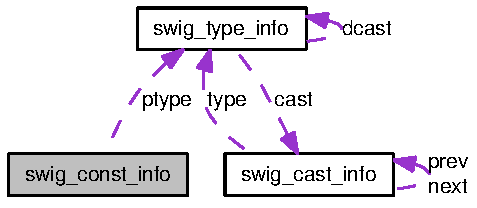
\includegraphics[width=265pt]{structswig__const__info__coll__graph}
\end{center}
\end{figure}
\subsection*{Data Fields}
\begin{CompactItemize}
\item 
int \hyperlink{structswig__const__info_c765329451135abec74c45e1897abf26}{type}
\item 
char $\ast$ \hyperlink{structswig__const__info_5ac083a645d964373f022d03df4849c8}{name}
\item 
long \hyperlink{structswig__const__info_d27f45c6331d8b6ac603e0cae235fb61}{lvalue}
\item 
double \hyperlink{structswig__const__info_b88920172b5a32b077bd95bb1f3d6f8e}{dvalue}
\item 
void $\ast$ \hyperlink{structswig__const__info_728d7ae5aaef6e9bdb0ec8a4e5c429b7}{pvalue}
\item 
\hyperlink{structswig__type__info}{swig\_\-type\_\-info} $\ast$$\ast$ \hyperlink{structswig__const__info_d55d59eb3cf7a2bb1fa92d92d42e782b}{ptype}
\end{CompactItemize}


\subsection{Detailed Description}


Definition at line 959 of file Lgm\_\-CTrans\_\-wrap.c.

\subsection{Field Documentation}
\hypertarget{structswig__const__info_c765329451135abec74c45e1897abf26}{
\index{swig\_\-const\_\-info@{swig\_\-const\_\-info}!type@{type}}
\index{type@{type}!swig_const_info@{swig\_\-const\_\-info}}
\subsubsection[{type}]{\setlength{\rightskip}{0pt plus 5cm}int {\bf type}}}
\label{structswig__const__info_c765329451135abec74c45e1897abf26}




Definition at line 960 of file Lgm\_\-CTrans\_\-wrap.c.\hypertarget{structswig__const__info_5ac083a645d964373f022d03df4849c8}{
\index{swig\_\-const\_\-info@{swig\_\-const\_\-info}!name@{name}}
\index{name@{name}!swig_const_info@{swig\_\-const\_\-info}}
\subsubsection[{name}]{\setlength{\rightskip}{0pt plus 5cm}char$\ast$ {\bf name}}}
\label{structswig__const__info_5ac083a645d964373f022d03df4849c8}




Definition at line 961 of file Lgm\_\-CTrans\_\-wrap.c.\hypertarget{structswig__const__info_d27f45c6331d8b6ac603e0cae235fb61}{
\index{swig\_\-const\_\-info@{swig\_\-const\_\-info}!lvalue@{lvalue}}
\index{lvalue@{lvalue}!swig_const_info@{swig\_\-const\_\-info}}
\subsubsection[{lvalue}]{\setlength{\rightskip}{0pt plus 5cm}long {\bf lvalue}}}
\label{structswig__const__info_d27f45c6331d8b6ac603e0cae235fb61}




Definition at line 962 of file Lgm\_\-CTrans\_\-wrap.c.\hypertarget{structswig__const__info_b88920172b5a32b077bd95bb1f3d6f8e}{
\index{swig\_\-const\_\-info@{swig\_\-const\_\-info}!dvalue@{dvalue}}
\index{dvalue@{dvalue}!swig_const_info@{swig\_\-const\_\-info}}
\subsubsection[{dvalue}]{\setlength{\rightskip}{0pt plus 5cm}double {\bf dvalue}}}
\label{structswig__const__info_b88920172b5a32b077bd95bb1f3d6f8e}




Definition at line 963 of file Lgm\_\-CTrans\_\-wrap.c.\hypertarget{structswig__const__info_728d7ae5aaef6e9bdb0ec8a4e5c429b7}{
\index{swig\_\-const\_\-info@{swig\_\-const\_\-info}!pvalue@{pvalue}}
\index{pvalue@{pvalue}!swig_const_info@{swig\_\-const\_\-info}}
\subsubsection[{pvalue}]{\setlength{\rightskip}{0pt plus 5cm}void$\ast$ {\bf pvalue}}}
\label{structswig__const__info_728d7ae5aaef6e9bdb0ec8a4e5c429b7}




Definition at line 964 of file Lgm\_\-CTrans\_\-wrap.c.\hypertarget{structswig__const__info_d55d59eb3cf7a2bb1fa92d92d42e782b}{
\index{swig\_\-const\_\-info@{swig\_\-const\_\-info}!ptype@{ptype}}
\index{ptype@{ptype}!swig_const_info@{swig\_\-const\_\-info}}
\subsubsection[{ptype}]{\setlength{\rightskip}{0pt plus 5cm}{\bf swig\_\-type\_\-info}$\ast$$\ast$ {\bf ptype}}}
\label{structswig__const__info_d55d59eb3cf7a2bb1fa92d92d42e782b}




Definition at line 965 of file Lgm\_\-CTrans\_\-wrap.c.

The documentation for this struct was generated from the following file:\begin{CompactItemize}
\item 
/home/mgh/LanlGeoMag/libLanlGeoMag/\hyperlink{_lgm___c_trans__wrap_8c}{Lgm\_\-CTrans\_\-wrap.c}\end{CompactItemize}

\hypertarget{structswig__globalvar}{
\section{swig\_\-globalvar Struct Reference}
\label{structswig__globalvar}\index{swig\_\-globalvar@{swig\_\-globalvar}}
}
Collaboration diagram for swig\_\-globalvar:\nopagebreak
\begin{figure}[H]
\begin{center}
\leavevmode
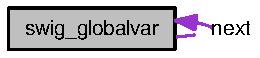
\includegraphics[width=161pt]{structswig__globalvar__coll__graph}
\end{center}
\end{figure}
\subsection*{Data Fields}
\begin{CompactItemize}
\item 
char $\ast$ \hyperlink{structswig__globalvar_5ac083a645d964373f022d03df4849c8}{name}
\item 
PyObject $\ast$($\ast$ \hyperlink{structswig__globalvar_0879d4d584d1ffda2ef5f917dc5a6f0a}{get\_\-attr} )(void)
\item 
int($\ast$ \hyperlink{structswig__globalvar_a452f906a54c91621799831e4280478f}{set\_\-attr} )(PyObject $\ast$)
\item 
struct \hyperlink{structswig__globalvar}{swig\_\-globalvar} $\ast$ \hyperlink{structswig__globalvar_caa8d5ee0bdeaf2c6975b8751dc580fa}{next}
\end{CompactItemize}


\subsection{Detailed Description}


Definition at line 12862 of file Lgm\_\-CTrans\_\-wrap.c.

\subsection{Field Documentation}
\hypertarget{structswig__globalvar_5ac083a645d964373f022d03df4849c8}{
\index{swig\_\-globalvar@{swig\_\-globalvar}!name@{name}}
\index{name@{name}!swig_globalvar@{swig\_\-globalvar}}
\subsubsection[{name}]{\setlength{\rightskip}{0pt plus 5cm}char$\ast$ {\bf name}}}
\label{structswig__globalvar_5ac083a645d964373f022d03df4849c8}




Definition at line 12863 of file Lgm\_\-CTrans\_\-wrap.c.\hypertarget{structswig__globalvar_0879d4d584d1ffda2ef5f917dc5a6f0a}{
\index{swig\_\-globalvar@{swig\_\-globalvar}!get\_\-attr@{get\_\-attr}}
\index{get\_\-attr@{get\_\-attr}!swig_globalvar@{swig\_\-globalvar}}
\subsubsection[{get\_\-attr}]{\setlength{\rightskip}{0pt plus 5cm}PyObject$\ast$($\ast$ {\bf get\_\-attr})(void)}}
\label{structswig__globalvar_0879d4d584d1ffda2ef5f917dc5a6f0a}


\hypertarget{structswig__globalvar_a452f906a54c91621799831e4280478f}{
\index{swig\_\-globalvar@{swig\_\-globalvar}!set\_\-attr@{set\_\-attr}}
\index{set\_\-attr@{set\_\-attr}!swig_globalvar@{swig\_\-globalvar}}
\subsubsection[{set\_\-attr}]{\setlength{\rightskip}{0pt plus 5cm}int($\ast$ {\bf set\_\-attr})(PyObject $\ast$)}}
\label{structswig__globalvar_a452f906a54c91621799831e4280478f}


\hypertarget{structswig__globalvar_caa8d5ee0bdeaf2c6975b8751dc580fa}{
\index{swig\_\-globalvar@{swig\_\-globalvar}!next@{next}}
\index{next@{next}!swig_globalvar@{swig\_\-globalvar}}
\subsubsection[{next}]{\setlength{\rightskip}{0pt plus 5cm}struct {\bf swig\_\-globalvar}$\ast$ {\bf next}\hspace{0.3cm}{\tt  \mbox{[}read\mbox{]}}}}
\label{structswig__globalvar_caa8d5ee0bdeaf2c6975b8751dc580fa}




Definition at line 12866 of file Lgm\_\-CTrans\_\-wrap.c.

The documentation for this struct was generated from the following file:\begin{CompactItemize}
\item 
/home/mgh/LanlGeoMag/libLanlGeoMag/\hyperlink{_lgm___c_trans__wrap_8c}{Lgm\_\-CTrans\_\-wrap.c}\end{CompactItemize}

\hypertarget{structswig__module__info}{
\section{swig\_\-module\_\-info Struct Reference}
\label{structswig__module__info}\index{swig\_\-module\_\-info@{swig\_\-module\_\-info}}
}
Collaboration diagram for swig\_\-module\_\-info:\nopagebreak
\begin{figure}[H]
\begin{center}
\leavevmode
\includegraphics[width=238pt]{structswig__module__info__coll__graph}
\end{center}
\end{figure}
\subsection*{Data Fields}
\begin{CompactItemize}
\item 
\hyperlink{structswig__type__info}{swig\_\-type\_\-info} $\ast$$\ast$ \hyperlink{structswig__module__info_b3f7a3650d62b94bd66b389d74eec755}{types}
\item 
size\_\-t \hyperlink{structswig__module__info_854352f53b148adc24983a58a1866d66}{size}
\item 
struct \hyperlink{structswig__module__info}{swig\_\-module\_\-info} $\ast$ \hyperlink{structswig__module__info_f0954fbff8a3ad66e8e856a4f544a3d9}{next}
\item 
\hyperlink{structswig__type__info}{swig\_\-type\_\-info} $\ast$$\ast$ \hyperlink{structswig__module__info_54e7d318722d57d376b4d394d254228f}{type\_\-initial}
\item 
\hyperlink{structswig__cast__info}{swig\_\-cast\_\-info} $\ast$$\ast$ \hyperlink{structswig__module__info_4185798e8e6242699bc018f9183a674c}{cast\_\-initial}
\item 
void $\ast$ \hyperlink{structswig__module__info_e60177f52d83fcd32268d79f2aa8012f}{clientdata}
\end{CompactItemize}


\subsection{Detailed Description}


Definition at line 335 of file Lgm\_\-CTrans\_\-wrap.c.

\subsection{Field Documentation}
\hypertarget{structswig__module__info_b3f7a3650d62b94bd66b389d74eec755}{
\index{swig\_\-module\_\-info@{swig\_\-module\_\-info}!types@{types}}
\index{types@{types}!swig_module_info@{swig\_\-module\_\-info}}
\subsubsection[{types}]{\setlength{\rightskip}{0pt plus 5cm}{\bf swig\_\-type\_\-info}$\ast$$\ast$ {\bf types}}}
\label{structswig__module__info_b3f7a3650d62b94bd66b389d74eec755}




Definition at line 336 of file Lgm\_\-CTrans\_\-wrap.c.\hypertarget{structswig__module__info_854352f53b148adc24983a58a1866d66}{
\index{swig\_\-module\_\-info@{swig\_\-module\_\-info}!size@{size}}
\index{size@{size}!swig_module_info@{swig\_\-module\_\-info}}
\subsubsection[{size}]{\setlength{\rightskip}{0pt plus 5cm}size\_\-t {\bf size}}}
\label{structswig__module__info_854352f53b148adc24983a58a1866d66}




Definition at line 337 of file Lgm\_\-CTrans\_\-wrap.c.\hypertarget{structswig__module__info_f0954fbff8a3ad66e8e856a4f544a3d9}{
\index{swig\_\-module\_\-info@{swig\_\-module\_\-info}!next@{next}}
\index{next@{next}!swig_module_info@{swig\_\-module\_\-info}}
\subsubsection[{next}]{\setlength{\rightskip}{0pt plus 5cm}struct {\bf swig\_\-module\_\-info}$\ast$ {\bf next}\hspace{0.3cm}{\tt  \mbox{[}read\mbox{]}}}}
\label{structswig__module__info_f0954fbff8a3ad66e8e856a4f544a3d9}




Definition at line 338 of file Lgm\_\-CTrans\_\-wrap.c.\hypertarget{structswig__module__info_54e7d318722d57d376b4d394d254228f}{
\index{swig\_\-module\_\-info@{swig\_\-module\_\-info}!type\_\-initial@{type\_\-initial}}
\index{type\_\-initial@{type\_\-initial}!swig_module_info@{swig\_\-module\_\-info}}
\subsubsection[{type\_\-initial}]{\setlength{\rightskip}{0pt plus 5cm}{\bf swig\_\-type\_\-info}$\ast$$\ast$ {\bf type\_\-initial}}}
\label{structswig__module__info_54e7d318722d57d376b4d394d254228f}




Definition at line 339 of file Lgm\_\-CTrans\_\-wrap.c.\hypertarget{structswig__module__info_4185798e8e6242699bc018f9183a674c}{
\index{swig\_\-module\_\-info@{swig\_\-module\_\-info}!cast\_\-initial@{cast\_\-initial}}
\index{cast\_\-initial@{cast\_\-initial}!swig_module_info@{swig\_\-module\_\-info}}
\subsubsection[{cast\_\-initial}]{\setlength{\rightskip}{0pt plus 5cm}{\bf swig\_\-cast\_\-info}$\ast$$\ast$ {\bf cast\_\-initial}}}
\label{structswig__module__info_4185798e8e6242699bc018f9183a674c}




Definition at line 340 of file Lgm\_\-CTrans\_\-wrap.c.\hypertarget{structswig__module__info_e60177f52d83fcd32268d79f2aa8012f}{
\index{swig\_\-module\_\-info@{swig\_\-module\_\-info}!clientdata@{clientdata}}
\index{clientdata@{clientdata}!swig_module_info@{swig\_\-module\_\-info}}
\subsubsection[{clientdata}]{\setlength{\rightskip}{0pt plus 5cm}void$\ast$ {\bf clientdata}}}
\label{structswig__module__info_e60177f52d83fcd32268d79f2aa8012f}




Definition at line 341 of file Lgm\_\-CTrans\_\-wrap.c.

The documentation for this struct was generated from the following file:\begin{CompactItemize}
\item 
/home/mgh/LanlGeoMag/libLanlGeoMag/\hyperlink{_lgm___c_trans__wrap_8c}{Lgm\_\-CTrans\_\-wrap.c}\end{CompactItemize}

\hypertarget{structswig__type__info}{
\section{swig\_\-type\_\-info Struct Reference}
\label{structswig__type__info}\index{swig\_\-type\_\-info@{swig\_\-type\_\-info}}
}
Collaboration diagram for swig\_\-type\_\-info:\nopagebreak
\begin{figure}[H]
\begin{center}
\leavevmode
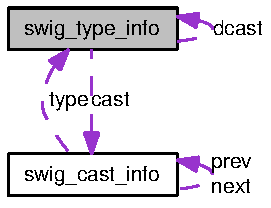
\includegraphics[width=166pt]{structswig__type__info__coll__graph}
\end{center}
\end{figure}
\subsection*{Data Fields}
\begin{CompactItemize}
\item 
const char $\ast$ \hyperlink{structswig__type__info_8f8f80d37794cde9472343e4487ba3eb}{name}
\item 
const char $\ast$ \hyperlink{structswig__type__info_f25d6dc49269fa2003ac7c7fa6f13915}{str}
\item 
\hyperlink{_lgm___c_trans__wrap_8c_d9f16e529633c78df7a780b9749395ce}{swig\_\-dycast\_\-func} \hyperlink{structswig__type__info_f97c463eb56e4061bd472750f8f501d3}{dcast}
\item 
struct \hyperlink{structswig__cast__info}{swig\_\-cast\_\-info} $\ast$ \hyperlink{structswig__type__info_ed90935b91e98b8de705d24f1b6facb0}{cast}
\item 
void $\ast$ \hyperlink{structswig__type__info_e60177f52d83fcd32268d79f2aa8012f}{clientdata}
\item 
int \hyperlink{structswig__type__info_25f6d5be66f731f527b185e361b06509}{owndata}
\end{CompactItemize}


\subsection{Detailed Description}


Definition at line 315 of file Lgm\_\-CTrans\_\-wrap.c.

\subsection{Field Documentation}
\hypertarget{structswig__type__info_8f8f80d37794cde9472343e4487ba3eb}{
\index{swig\_\-type\_\-info@{swig\_\-type\_\-info}!name@{name}}
\index{name@{name}!swig_type_info@{swig\_\-type\_\-info}}
\subsubsection[{name}]{\setlength{\rightskip}{0pt plus 5cm}const char$\ast$ {\bf name}}}
\label{structswig__type__info_8f8f80d37794cde9472343e4487ba3eb}




Definition at line 316 of file Lgm\_\-CTrans\_\-wrap.c.\hypertarget{structswig__type__info_f25d6dc49269fa2003ac7c7fa6f13915}{
\index{swig\_\-type\_\-info@{swig\_\-type\_\-info}!str@{str}}
\index{str@{str}!swig_type_info@{swig\_\-type\_\-info}}
\subsubsection[{str}]{\setlength{\rightskip}{0pt plus 5cm}const char$\ast$ {\bf str}}}
\label{structswig__type__info_f25d6dc49269fa2003ac7c7fa6f13915}




Definition at line 317 of file Lgm\_\-CTrans\_\-wrap.c.\hypertarget{structswig__type__info_f97c463eb56e4061bd472750f8f501d3}{
\index{swig\_\-type\_\-info@{swig\_\-type\_\-info}!dcast@{dcast}}
\index{dcast@{dcast}!swig_type_info@{swig\_\-type\_\-info}}
\subsubsection[{dcast}]{\setlength{\rightskip}{0pt plus 5cm}{\bf swig\_\-dycast\_\-func} {\bf dcast}}}
\label{structswig__type__info_f97c463eb56e4061bd472750f8f501d3}




Definition at line 318 of file Lgm\_\-CTrans\_\-wrap.c.\hypertarget{structswig__type__info_ed90935b91e98b8de705d24f1b6facb0}{
\index{swig\_\-type\_\-info@{swig\_\-type\_\-info}!cast@{cast}}
\index{cast@{cast}!swig_type_info@{swig\_\-type\_\-info}}
\subsubsection[{cast}]{\setlength{\rightskip}{0pt plus 5cm}struct {\bf swig\_\-cast\_\-info}$\ast$ {\bf cast}\hspace{0.3cm}{\tt  \mbox{[}read\mbox{]}}}}
\label{structswig__type__info_ed90935b91e98b8de705d24f1b6facb0}




Definition at line 319 of file Lgm\_\-CTrans\_\-wrap.c.\hypertarget{structswig__type__info_e60177f52d83fcd32268d79f2aa8012f}{
\index{swig\_\-type\_\-info@{swig\_\-type\_\-info}!clientdata@{clientdata}}
\index{clientdata@{clientdata}!swig_type_info@{swig\_\-type\_\-info}}
\subsubsection[{clientdata}]{\setlength{\rightskip}{0pt plus 5cm}void$\ast$ {\bf clientdata}}}
\label{structswig__type__info_e60177f52d83fcd32268d79f2aa8012f}




Definition at line 320 of file Lgm\_\-CTrans\_\-wrap.c.\hypertarget{structswig__type__info_25f6d5be66f731f527b185e361b06509}{
\index{swig\_\-type\_\-info@{swig\_\-type\_\-info}!owndata@{owndata}}
\index{owndata@{owndata}!swig_type_info@{swig\_\-type\_\-info}}
\subsubsection[{owndata}]{\setlength{\rightskip}{0pt plus 5cm}int {\bf owndata}}}
\label{structswig__type__info_25f6d5be66f731f527b185e361b06509}




Definition at line 321 of file Lgm\_\-CTrans\_\-wrap.c.

The documentation for this struct was generated from the following file:\begin{CompactItemize}
\item 
/home/mgh/LanlGeoMag/libLanlGeoMag/\hyperlink{_lgm___c_trans__wrap_8c}{Lgm\_\-CTrans\_\-wrap.c}\end{CompactItemize}

\hypertarget{structswig__varlinkobject}{
\section{swig\_\-varlinkobject Struct Reference}
\label{structswig__varlinkobject}\index{swig\_\-varlinkobject@{swig\_\-varlinkobject}}
}
Collaboration diagram for swig\_\-varlinkobject:\nopagebreak
\begin{figure}[H]
\begin{center}
\leavevmode
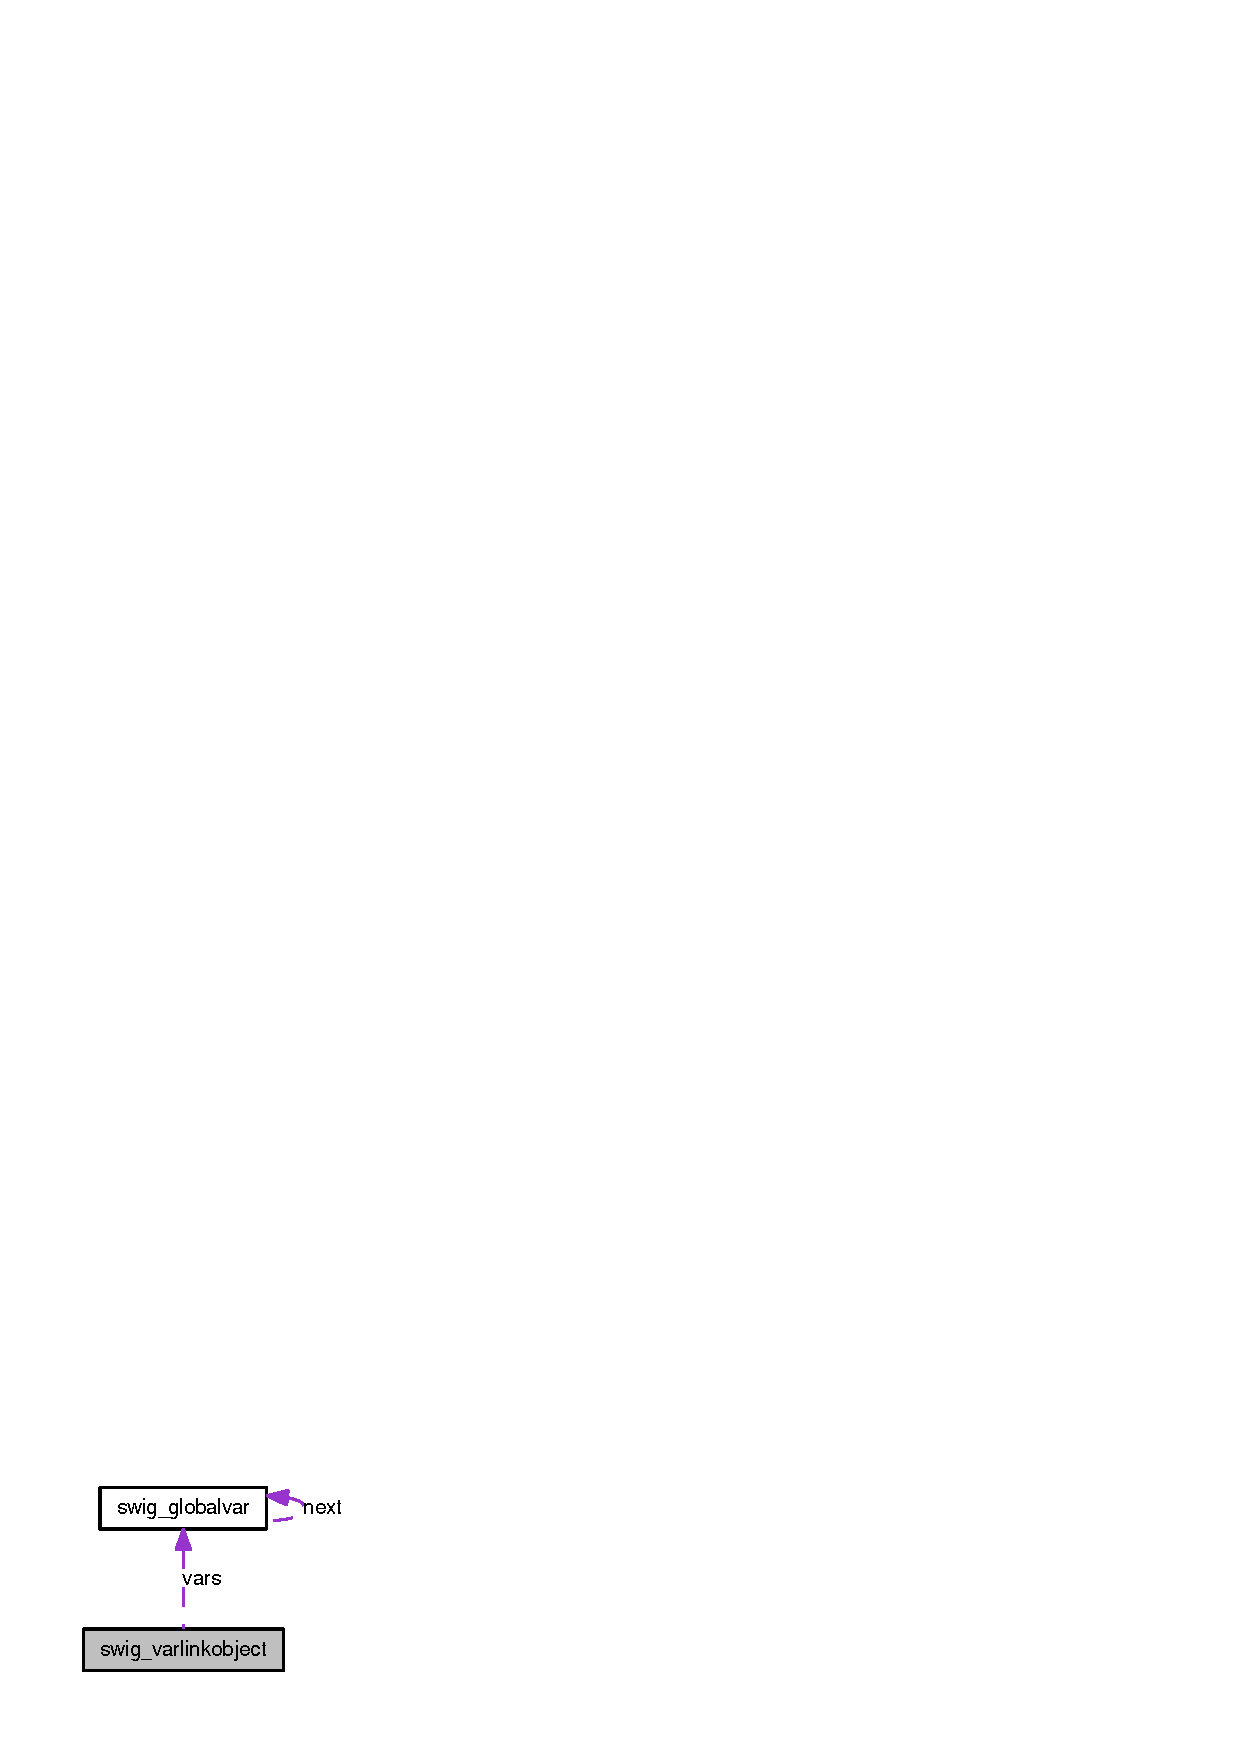
\includegraphics[width=169pt]{structswig__varlinkobject__coll__graph}
\end{center}
\end{figure}
\subsection*{Data Fields}
\begin{CompactItemize}
\item 
PyObject\_\-HEAD \hyperlink{structswig__globalvar}{swig\_\-globalvar} $\ast$ \hyperlink{structswig__varlinkobject_64a30a7c2383b2e2a7bd8aeb3e492449}{vars}
\end{CompactItemize}


\subsection{Detailed Description}


Definition at line 12869 of file Lgm\_\-CTrans\_\-wrap.c.

\subsection{Field Documentation}
\hypertarget{structswig__varlinkobject_64a30a7c2383b2e2a7bd8aeb3e492449}{
\index{swig\_\-varlinkobject@{swig\_\-varlinkobject}!vars@{vars}}
\index{vars@{vars}!swig_varlinkobject@{swig\_\-varlinkobject}}
\subsubsection[{vars}]{\setlength{\rightskip}{0pt plus 5cm}PyObject\_\-HEAD {\bf swig\_\-globalvar}$\ast$ {\bf vars}}}
\label{structswig__varlinkobject_64a30a7c2383b2e2a7bd8aeb3e492449}




Definition at line 12871 of file Lgm\_\-CTrans\_\-wrap.c.

The documentation for this struct was generated from the following file:\begin{CompactItemize}
\item 
/home/mgh/LanlGeoMag/libLanlGeoMag/\hyperlink{_lgm___c_trans__wrap_8c}{Lgm\_\-CTrans\_\-wrap.c}\end{CompactItemize}

\chapter{File Documentation}
\hypertarget{_alpha_of_k_8c}{
\section{/home/mgh/LanlGeoMag/libLanlGeoMag/AlphaOfK.c File Reference}
\label{_alpha_of_k_8c}\index{/home/mgh/LanlGeoMag/libLanlGeoMag/AlphaOfK.c@{/home/mgh/LanlGeoMag/libLanlGeoMag/AlphaOfK.c}}
}
{\tt \#include $<$stdio.h$>$}\par
{\tt \#include $<$math.h$>$}\par
{\tt \#include \char`\"{}Lgm/Lgm\_\-QuadPack.h\char`\"{}}\par
{\tt \#include \char`\"{}Lgm/Lgm\_\-MagModelInfo.h\char`\"{}}\par
{\tt \#include \char`\"{}Lgm/Lgm\_\-LstarInfo.h\char`\"{}}\par
{\tt \#include $<$gsl/gsl\_\-errno.h$>$}\par
{\tt \#include $<$gsl/gsl\_\-spline.h$>$}\par
{\tt \#include $<$string.h$>$}\par


Include dependency graph for AlphaOfK.c:\nopagebreak
\begin{figure}[H]
\begin{center}
\leavevmode
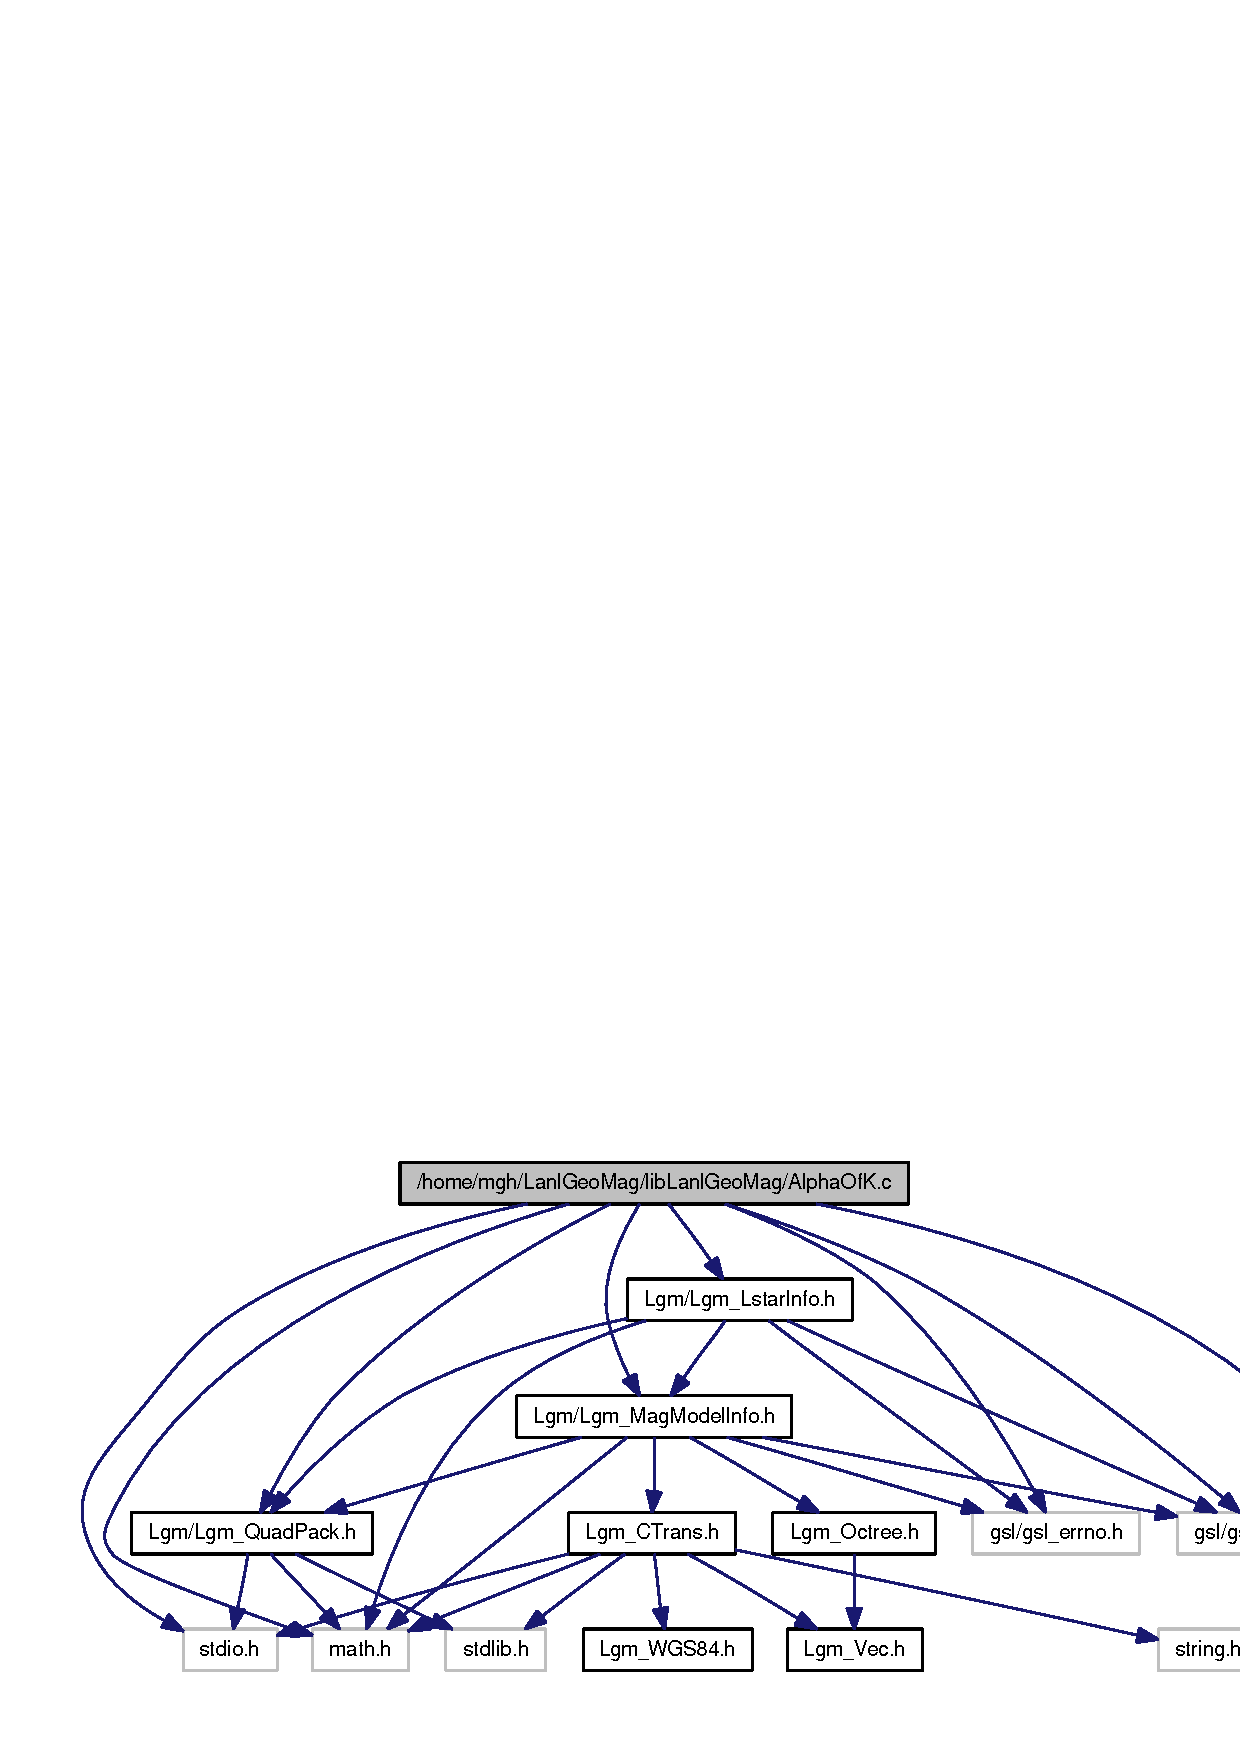
\includegraphics[width=331pt]{_alpha_of_k_8c__incl}
\end{center}
\end{figure}
\subsection*{Defines}
\begin{CompactItemize}
\item 
\#define \hyperlink{_alpha_of_k_8c_5ce702bb9d0edd19fbb1d576cfaf7010}{TRACE\_\-TOL}~1e-7
\item 
\#define \hyperlink{_alpha_of_k_8c_f468028083c9e52aa2c94ef3b9940450}{GOLD}~0.38197
\end{CompactItemize}
\subsection*{Functions}
\begin{CompactItemize}
\item 
double \hyperlink{_alpha_of_k_8c_8c0c461cb66bea86f5c7703017a24dde}{Func} (double Kt, double Alpha, \hyperlink{struct_lgm___lstar_info}{Lgm\_\-LstarInfo} $\ast$LstarInfo)
\item 
double \hyperlink{_alpha_of_k_8c_a9a43909d59850c622768267ce73421c}{AlphaOfK} (double K, \hyperlink{struct_lgm___lstar_info}{Lgm\_\-LstarInfo} $\ast$LstarInfo)
\end{CompactItemize}


\subsection{Define Documentation}
\hypertarget{_alpha_of_k_8c_5ce702bb9d0edd19fbb1d576cfaf7010}{
\index{AlphaOfK.c@{AlphaOfK.c}!TRACE\_\-TOL@{TRACE\_\-TOL}}
\index{TRACE\_\-TOL@{TRACE\_\-TOL}!AlphaOfK.c@{AlphaOfK.c}}
\subsubsection[{TRACE\_\-TOL}]{\setlength{\rightskip}{0pt plus 5cm}\#define TRACE\_\-TOL~1e-7}}
\label{_alpha_of_k_8c_5ce702bb9d0edd19fbb1d576cfaf7010}




Definition at line 10 of file AlphaOfK.c.\hypertarget{_alpha_of_k_8c_f468028083c9e52aa2c94ef3b9940450}{
\index{AlphaOfK.c@{AlphaOfK.c}!GOLD@{GOLD}}
\index{GOLD@{GOLD}!AlphaOfK.c@{AlphaOfK.c}}
\subsubsection[{GOLD}]{\setlength{\rightskip}{0pt plus 5cm}\#define GOLD~0.38197}}
\label{_alpha_of_k_8c_f468028083c9e52aa2c94ef3b9940450}




Definition at line 11 of file AlphaOfK.c.

\subsection{Function Documentation}
\hypertarget{_alpha_of_k_8c_8c0c461cb66bea86f5c7703017a24dde}{
\index{AlphaOfK.c@{AlphaOfK.c}!Func@{Func}}
\index{Func@{Func}!AlphaOfK.c@{AlphaOfK.c}}
\subsubsection[{Func}]{\setlength{\rightskip}{0pt plus 5cm}double Func (double {\em Kt}, \/  double {\em Alpha}, \/  {\bf Lgm\_\-LstarInfo} $\ast$ {\em LstarInfo})}}
\label{_alpha_of_k_8c_8c0c461cb66bea86f5c7703017a24dde}




Definition at line 109 of file AlphaOfK.c.

Here is the call graph for this function:\nopagebreak
\begin{figure}[H]
\begin{center}
\leavevmode
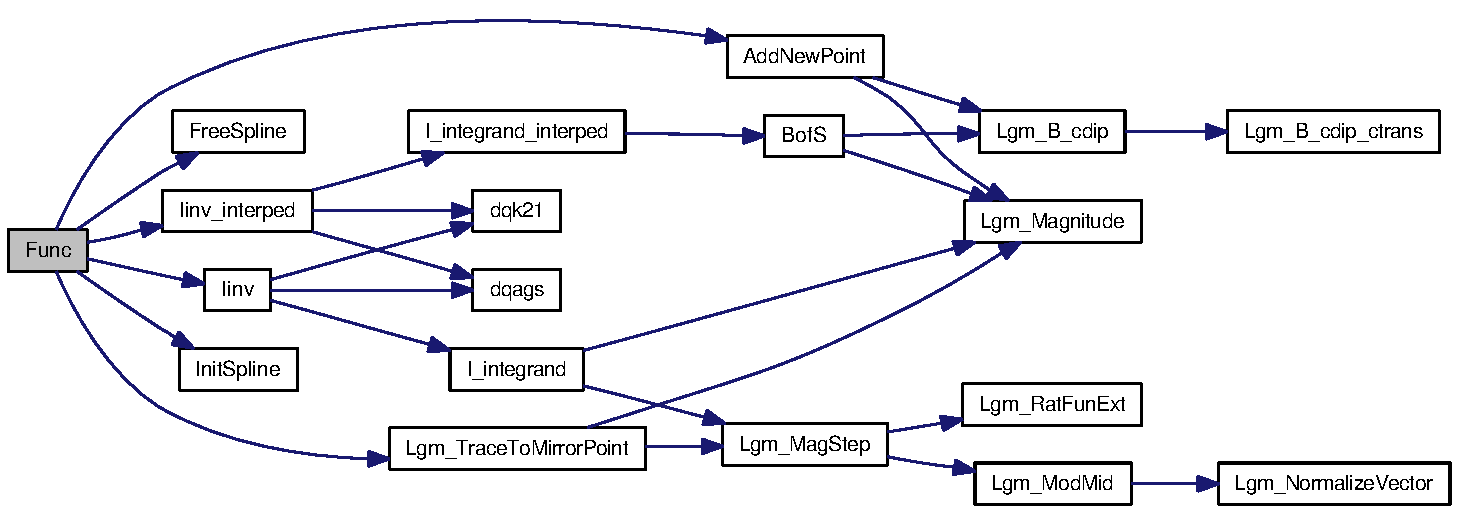
\includegraphics[width=368pt]{_alpha_of_k_8c_8c0c461cb66bea86f5c7703017a24dde_cgraph}
\end{center}
\end{figure}


Here is the caller graph for this function:\nopagebreak
\begin{figure}[H]
\begin{center}
\leavevmode
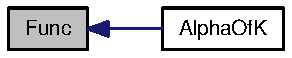
\includegraphics[width=88pt]{_alpha_of_k_8c_8c0c461cb66bea86f5c7703017a24dde_icgraph}
\end{center}
\end{figure}
\hypertarget{_alpha_of_k_8c_a9a43909d59850c622768267ce73421c}{
\index{AlphaOfK.c@{AlphaOfK.c}!AlphaOfK@{AlphaOfK}}
\index{AlphaOfK@{AlphaOfK}!AlphaOfK.c@{AlphaOfK.c}}
\subsubsection[{AlphaOfK}]{\setlength{\rightskip}{0pt plus 5cm}double AlphaOfK (double {\em K}, \/  {\bf Lgm\_\-LstarInfo} $\ast$ {\em LstarInfo})}}
\label{_alpha_of_k_8c_a9a43909d59850c622768267ce73421c}




Definition at line 24 of file AlphaOfK.c.

Here is the call graph for this function:\nopagebreak
\begin{figure}[H]
\begin{center}
\leavevmode
\includegraphics[width=415pt]{_alpha_of_k_8c_a9a43909d59850c622768267ce73421c_cgraph}
\end{center}
\end{figure}

\hypertarget{_b___from_scattered_data_8c}{
\section{/home/mgh/LanlGeoMag/libLanlGeoMag/B\_\-FromScatteredData.c File Reference}
\label{_b___from_scattered_data_8c}\index{/home/mgh/LanlGeoMag/libLanlGeoMag/B\_\-FromScatteredData.c@{/home/mgh/LanlGeoMag/libLanlGeoMag/B\_\-FromScatteredData.c}}
}
{\tt \#include \char`\"{}Lgm/Lgm\_\-MagModelInfo.h\char`\"{}}\par
{\tt \#include \char`\"{}Lgm/Lgm\_\-Octree.h\char`\"{}}\par
{\tt \#include $<$stdlib.h$>$}\par
{\tt \#include $<$gsl/gsl\_\-matrix.h$>$}\par
{\tt \#include $<$gsl/gsl\_\-linalg.h$>$}\par


Include dependency graph for B\_\-FromScatteredData.c:\nopagebreak
\begin{figure}[H]
\begin{center}
\leavevmode
\includegraphics[width=420pt]{_b___from_scattered_data_8c__incl}
\end{center}
\end{figure}
\subsection*{Functions}
\begin{CompactItemize}
\item 
void \hyperlink{_b___from_scattered_data_8c_471b3b6d51257ae76e4a22fa1d2e6f67}{DFI\_\-BasisFuncLin} (double $\ast$b, \hyperlink{struct_lgm___vector}{Lgm\_\-Vector} $\ast$P)
\item 
void \hyperlink{_b___from_scattered_data_8c_373301cb1510ec76bf04e60f44cc26fa}{DFI\_\-FuncLin} (\hyperlink{struct_lgm___vector}{Lgm\_\-Vector} $\ast$P, gsl\_\-vector $\ast$C, \hyperlink{struct_lgm___vector}{Lgm\_\-Vector} $\ast$V)
\item 
void \hyperlink{_b___from_scattered_data_8c_63e1b24396d764119a3d822773af07cb}{DFI\_\-DivBasisFuncLin} (double $\ast$bdiv, \hyperlink{struct_lgm___vector}{Lgm\_\-Vector} $\ast$P)
\item 
void \hyperlink{_b___from_scattered_data_8c_9133efa4bdfaeed11bba2e75d25f29cf}{DFI\_\-BasisFunc} (double $\ast$b, \hyperlink{struct_lgm___vector}{Lgm\_\-Vector} $\ast$P)
\item 
void \hyperlink{_b___from_scattered_data_8c_3b380e0805c4cf987f1c07da8759ff86}{DFI\_\-Func} (\hyperlink{struct_lgm___vector}{Lgm\_\-Vector} $\ast$P, gsl\_\-vector $\ast$C, \hyperlink{struct_lgm___vector}{Lgm\_\-Vector} $\ast$V)
\item 
void \hyperlink{_b___from_scattered_data_8c_f267e6c987d5ca7607b0ad4af4d1b783}{DFI\_\-DivBasisFunc} (double $\ast$bdiv, \hyperlink{struct_lgm___vector}{Lgm\_\-Vector} $\ast$P)
\item 
int \hyperlink{_b___from_scattered_data_8c_d11ba2ce714d9d6e4b6dc532fabe87c9}{Lgm\_\-DivFreeInterp} (\hyperlink{struct_lgm___vector}{Lgm\_\-Vector} $\ast$q, \hyperlink{struct___lgm___octree_data}{Lgm\_\-OctreeData} $\ast$kNN, int K, \hyperlink{struct_lgm___vector}{Lgm\_\-Vector} $\ast$v)
\item 
int \hyperlink{_b___from_scattered_data_8c_b67853a5a2e18a5e252ffbe4ac3c9ea6}{Lgm\_\-DivFreeInterp2} (\hyperlink{struct_lgm___vector}{Lgm\_\-Vector} $\ast$q, \hyperlink{struct___lgm___octree_data}{Lgm\_\-OctreeData} $\ast$kNN, int K, \hyperlink{struct_lgm___vector}{Lgm\_\-Vector} $\ast$v)
\item 
int \hyperlink{_b___from_scattered_data_8c_5138e7f3fa8a67aa8ab528ba9cd606d2}{Lgm\_\-B\_\-FromScatteredData} (\hyperlink{struct_lgm___vector}{Lgm\_\-Vector} $\ast$v, \hyperlink{struct_lgm___vector}{Lgm\_\-Vector} $\ast$B, \hyperlink{struct_lgm___mag_model_info}{Lgm\_\-MagModelInfo} $\ast$Info)
\end{CompactItemize}


\subsection{Function Documentation}
\hypertarget{_b___from_scattered_data_8c_471b3b6d51257ae76e4a22fa1d2e6f67}{
\index{B\_\-FromScatteredData.c@{B\_\-FromScatteredData.c}!DFI\_\-BasisFuncLin@{DFI\_\-BasisFuncLin}}
\index{DFI\_\-BasisFuncLin@{DFI\_\-BasisFuncLin}!B_FromScatteredData.c@{B\_\-FromScatteredData.c}}
\subsubsection[{DFI\_\-BasisFuncLin}]{\setlength{\rightskip}{0pt plus 5cm}void DFI\_\-BasisFuncLin (double $\ast$ {\em b}, \/  {\bf Lgm\_\-Vector} $\ast$ {\em P})}}
\label{_b___from_scattered_data_8c_471b3b6d51257ae76e4a22fa1d2e6f67}




Definition at line 28 of file B\_\-FromScatteredData.c.

Here is the caller graph for this function:\nopagebreak
\begin{figure}[H]
\begin{center}
\leavevmode
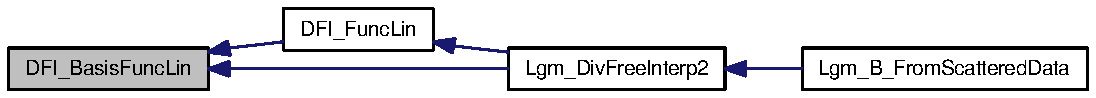
\includegraphics[width=281pt]{_b___from_scattered_data_8c_471b3b6d51257ae76e4a22fa1d2e6f67_icgraph}
\end{center}
\end{figure}
\hypertarget{_b___from_scattered_data_8c_373301cb1510ec76bf04e60f44cc26fa}{
\index{B\_\-FromScatteredData.c@{B\_\-FromScatteredData.c}!DFI\_\-FuncLin@{DFI\_\-FuncLin}}
\index{DFI\_\-FuncLin@{DFI\_\-FuncLin}!B_FromScatteredData.c@{B\_\-FromScatteredData.c}}
\subsubsection[{DFI\_\-FuncLin}]{\setlength{\rightskip}{0pt plus 5cm}void DFI\_\-FuncLin ({\bf Lgm\_\-Vector} $\ast$ {\em P}, \/  gsl\_\-vector $\ast$ {\em C}, \/  {\bf Lgm\_\-Vector} $\ast$ {\em V})}}
\label{_b___from_scattered_data_8c_373301cb1510ec76bf04e60f44cc26fa}




Definition at line 32 of file B\_\-FromScatteredData.c.

Here is the call graph for this function:\nopagebreak
\begin{figure}[H]
\begin{center}
\leavevmode
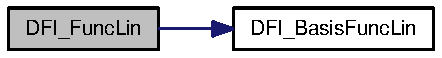
\includegraphics[width=124pt]{_b___from_scattered_data_8c_373301cb1510ec76bf04e60f44cc26fa_cgraph}
\end{center}
\end{figure}


Here is the caller graph for this function:\nopagebreak
\begin{figure}[H]
\begin{center}
\leavevmode
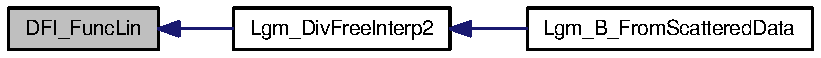
\includegraphics[width=215pt]{_b___from_scattered_data_8c_373301cb1510ec76bf04e60f44cc26fa_icgraph}
\end{center}
\end{figure}
\hypertarget{_b___from_scattered_data_8c_63e1b24396d764119a3d822773af07cb}{
\index{B\_\-FromScatteredData.c@{B\_\-FromScatteredData.c}!DFI\_\-DivBasisFuncLin@{DFI\_\-DivBasisFuncLin}}
\index{DFI\_\-DivBasisFuncLin@{DFI\_\-DivBasisFuncLin}!B_FromScatteredData.c@{B\_\-FromScatteredData.c}}
\subsubsection[{DFI\_\-DivBasisFuncLin}]{\setlength{\rightskip}{0pt plus 5cm}void DFI\_\-DivBasisFuncLin (double $\ast$ {\em bdiv}, \/  {\bf Lgm\_\-Vector} $\ast$ {\em P})}}
\label{_b___from_scattered_data_8c_63e1b24396d764119a3d822773af07cb}




Definition at line 42 of file B\_\-FromScatteredData.c.

Here is the caller graph for this function:\nopagebreak
\begin{figure}[H]
\begin{center}
\leavevmode
\includegraphics[width=235pt]{_b___from_scattered_data_8c_63e1b24396d764119a3d822773af07cb_icgraph}
\end{center}
\end{figure}
\hypertarget{_b___from_scattered_data_8c_9133efa4bdfaeed11bba2e75d25f29cf}{
\index{B\_\-FromScatteredData.c@{B\_\-FromScatteredData.c}!DFI\_\-BasisFunc@{DFI\_\-BasisFunc}}
\index{DFI\_\-BasisFunc@{DFI\_\-BasisFunc}!B_FromScatteredData.c@{B\_\-FromScatteredData.c}}
\subsubsection[{DFI\_\-BasisFunc}]{\setlength{\rightskip}{0pt plus 5cm}void DFI\_\-BasisFunc (double $\ast$ {\em b}, \/  {\bf Lgm\_\-Vector} $\ast$ {\em P})}}
\label{_b___from_scattered_data_8c_9133efa4bdfaeed11bba2e75d25f29cf}




Definition at line 58 of file B\_\-FromScatteredData.c.

Here is the caller graph for this function:\nopagebreak
\begin{figure}[H]
\begin{center}
\leavevmode
\includegraphics[width=267pt]{_b___from_scattered_data_8c_9133efa4bdfaeed11bba2e75d25f29cf_icgraph}
\end{center}
\end{figure}
\hypertarget{_b___from_scattered_data_8c_3b380e0805c4cf987f1c07da8759ff86}{
\index{B\_\-FromScatteredData.c@{B\_\-FromScatteredData.c}!DFI\_\-Func@{DFI\_\-Func}}
\index{DFI\_\-Func@{DFI\_\-Func}!B_FromScatteredData.c@{B\_\-FromScatteredData.c}}
\subsubsection[{DFI\_\-Func}]{\setlength{\rightskip}{0pt plus 5cm}void DFI\_\-Func ({\bf Lgm\_\-Vector} $\ast$ {\em P}, \/  gsl\_\-vector $\ast$ {\em C}, \/  {\bf Lgm\_\-Vector} $\ast$ {\em V})}}
\label{_b___from_scattered_data_8c_3b380e0805c4cf987f1c07da8759ff86}




Definition at line 65 of file B\_\-FromScatteredData.c.

Here is the call graph for this function:\nopagebreak
\begin{figure}[H]
\begin{center}
\leavevmode
\includegraphics[width=112pt]{_b___from_scattered_data_8c_3b380e0805c4cf987f1c07da8759ff86_cgraph}
\end{center}
\end{figure}


Here is the caller graph for this function:\nopagebreak
\begin{figure}[H]
\begin{center}
\leavevmode
\includegraphics[width=207pt]{_b___from_scattered_data_8c_3b380e0805c4cf987f1c07da8759ff86_icgraph}
\end{center}
\end{figure}
\hypertarget{_b___from_scattered_data_8c_f267e6c987d5ca7607b0ad4af4d1b783}{
\index{B\_\-FromScatteredData.c@{B\_\-FromScatteredData.c}!DFI\_\-DivBasisFunc@{DFI\_\-DivBasisFunc}}
\index{DFI\_\-DivBasisFunc@{DFI\_\-DivBasisFunc}!B_FromScatteredData.c@{B\_\-FromScatteredData.c}}
\subsubsection[{DFI\_\-DivBasisFunc}]{\setlength{\rightskip}{0pt plus 5cm}void DFI\_\-DivBasisFunc (double $\ast$ {\em bdiv}, \/  {\bf Lgm\_\-Vector} $\ast$ {\em P})}}
\label{_b___from_scattered_data_8c_f267e6c987d5ca7607b0ad4af4d1b783}




Definition at line 79 of file B\_\-FromScatteredData.c.\hypertarget{_b___from_scattered_data_8c_d11ba2ce714d9d6e4b6dc532fabe87c9}{
\index{B\_\-FromScatteredData.c@{B\_\-FromScatteredData.c}!Lgm\_\-DivFreeInterp@{Lgm\_\-DivFreeInterp}}
\index{Lgm\_\-DivFreeInterp@{Lgm\_\-DivFreeInterp}!B_FromScatteredData.c@{B\_\-FromScatteredData.c}}
\subsubsection[{Lgm\_\-DivFreeInterp}]{\setlength{\rightskip}{0pt plus 5cm}int Lgm\_\-DivFreeInterp ({\bf Lgm\_\-Vector} $\ast$ {\em q}, \/  {\bf Lgm\_\-OctreeData} $\ast$ {\em kNN}, \/  int {\em K}, \/  {\bf Lgm\_\-Vector} $\ast$ {\em v})}}
\label{_b___from_scattered_data_8c_d11ba2ce714d9d6e4b6dc532fabe87c9}




Definition at line 93 of file B\_\-FromScatteredData.c.

Here is the call graph for this function:\nopagebreak
\begin{figure}[H]
\begin{center}
\leavevmode
\includegraphics[width=180pt]{_b___from_scattered_data_8c_d11ba2ce714d9d6e4b6dc532fabe87c9_cgraph}
\end{center}
\end{figure}


Here is the caller graph for this function:\nopagebreak
\begin{figure}[H]
\begin{center}
\leavevmode
\includegraphics[width=159pt]{_b___from_scattered_data_8c_d11ba2ce714d9d6e4b6dc532fabe87c9_icgraph}
\end{center}
\end{figure}
\hypertarget{_b___from_scattered_data_8c_b67853a5a2e18a5e252ffbe4ac3c9ea6}{
\index{B\_\-FromScatteredData.c@{B\_\-FromScatteredData.c}!Lgm\_\-DivFreeInterp2@{Lgm\_\-DivFreeInterp2}}
\index{Lgm\_\-DivFreeInterp2@{Lgm\_\-DivFreeInterp2}!B_FromScatteredData.c@{B\_\-FromScatteredData.c}}
\subsubsection[{Lgm\_\-DivFreeInterp2}]{\setlength{\rightskip}{0pt plus 5cm}int Lgm\_\-DivFreeInterp2 ({\bf Lgm\_\-Vector} $\ast$ {\em q}, \/  {\bf Lgm\_\-OctreeData} $\ast$ {\em kNN}, \/  int {\em K}, \/  {\bf Lgm\_\-Vector} $\ast$ {\em v})}}
\label{_b___from_scattered_data_8c_b67853a5a2e18a5e252ffbe4ac3c9ea6}




Definition at line 294 of file B\_\-FromScatteredData.c.

Here is the call graph for this function:\nopagebreak
\begin{figure}[H]
\begin{center}
\leavevmode
\includegraphics[width=214pt]{_b___from_scattered_data_8c_b67853a5a2e18a5e252ffbe4ac3c9ea6_cgraph}
\end{center}
\end{figure}


Here is the caller graph for this function:\nopagebreak
\begin{figure}[H]
\begin{center}
\leavevmode
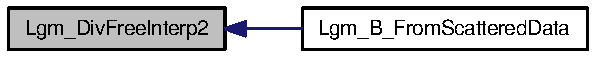
\includegraphics[width=161pt]{_b___from_scattered_data_8c_b67853a5a2e18a5e252ffbe4ac3c9ea6_icgraph}
\end{center}
\end{figure}
\hypertarget{_b___from_scattered_data_8c_5138e7f3fa8a67aa8ab528ba9cd606d2}{
\index{B\_\-FromScatteredData.c@{B\_\-FromScatteredData.c}!Lgm\_\-B\_\-FromScatteredData@{Lgm\_\-B\_\-FromScatteredData}}
\index{Lgm\_\-B\_\-FromScatteredData@{Lgm\_\-B\_\-FromScatteredData}!B_FromScatteredData.c@{B\_\-FromScatteredData.c}}
\subsubsection[{Lgm\_\-B\_\-FromScatteredData}]{\setlength{\rightskip}{0pt plus 5cm}int Lgm\_\-B\_\-FromScatteredData ({\bf Lgm\_\-Vector} $\ast$ {\em v}, \/  {\bf Lgm\_\-Vector} $\ast$ {\em B}, \/  {\bf Lgm\_\-MagModelInfo} $\ast$ {\em Info})}}
\label{_b___from_scattered_data_8c_5138e7f3fa8a67aa8ab528ba9cd606d2}




Definition at line 448 of file B\_\-FromScatteredData.c.

Here is the call graph for this function:\nopagebreak
\begin{figure}[H]
\begin{center}
\leavevmode
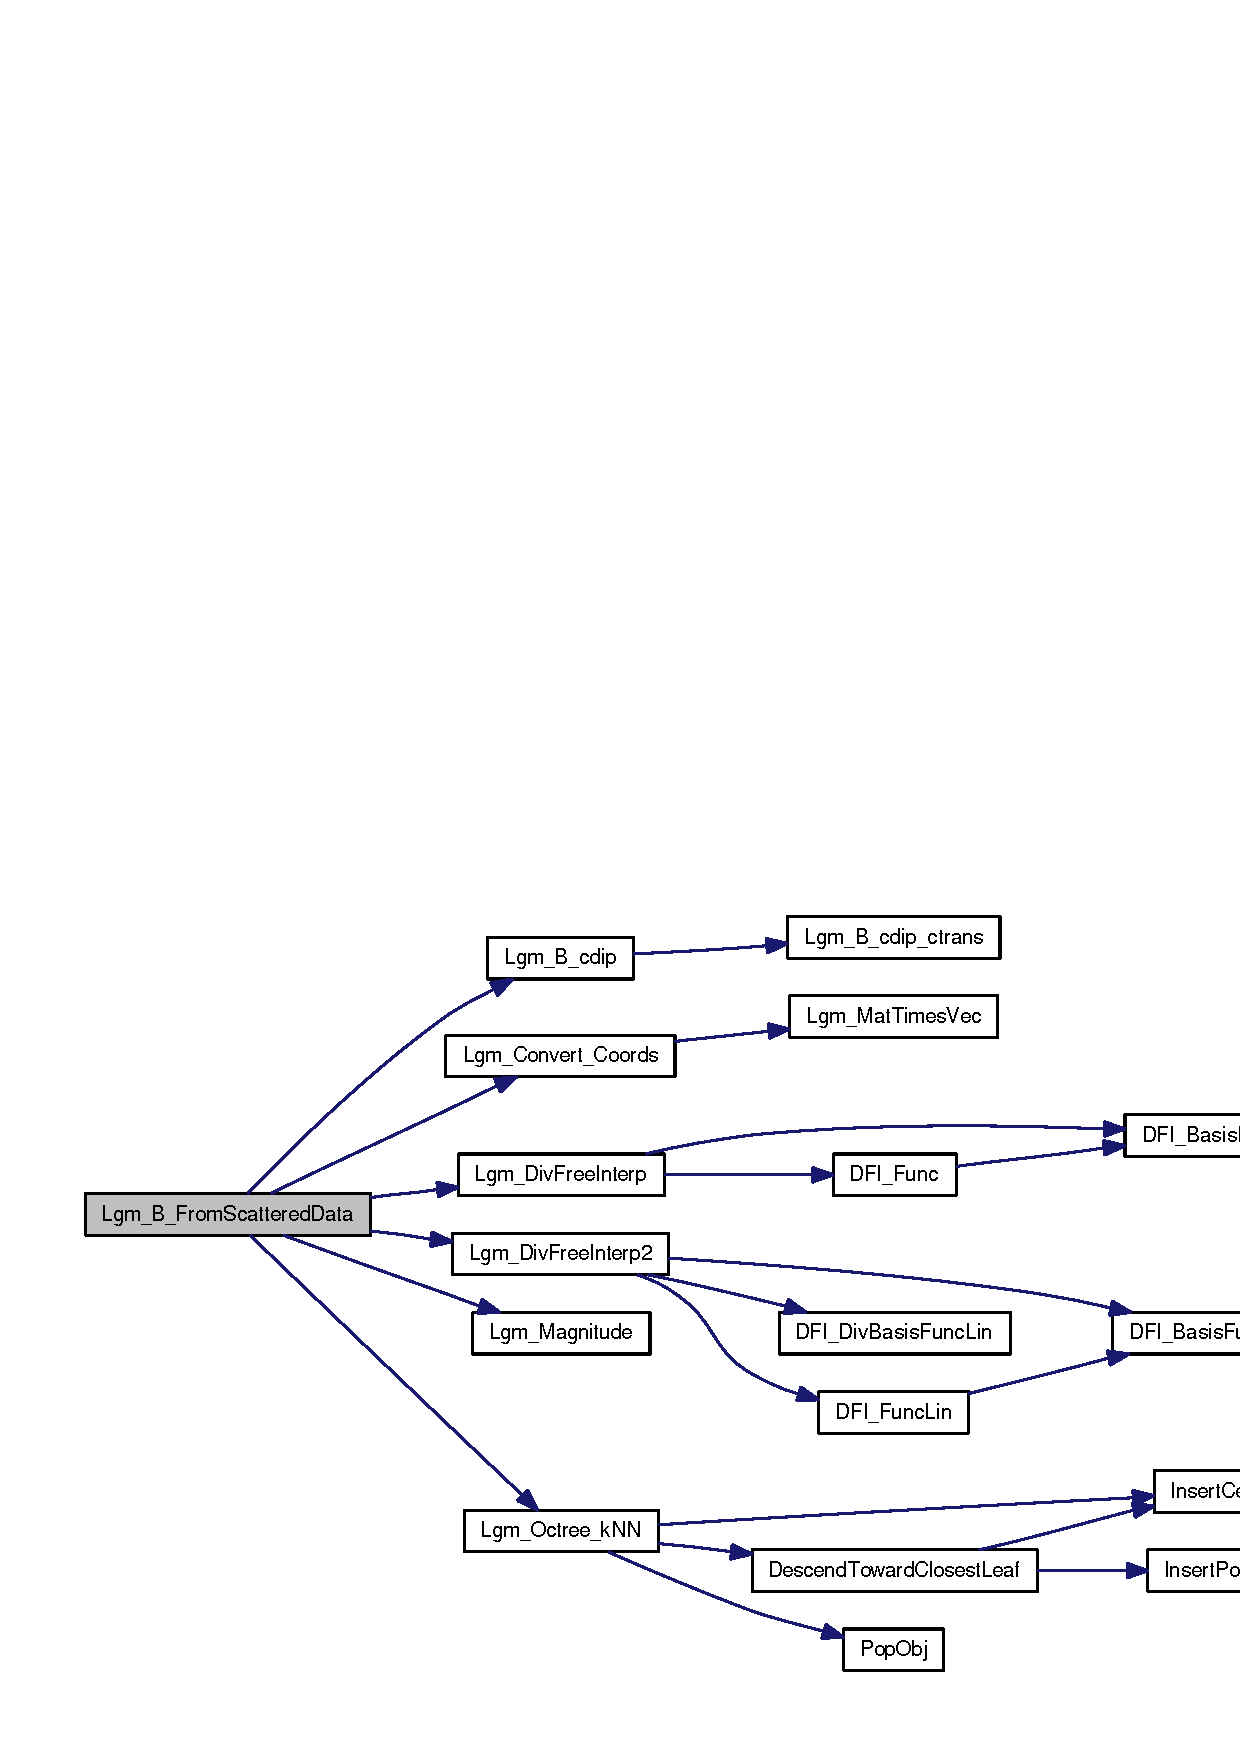
\includegraphics[width=360pt]{_b___from_scattered_data_8c_5138e7f3fa8a67aa8ab528ba9cd606d2_cgraph}
\end{center}
\end{figure}

\hypertarget{_compute_lstar_8c}{
\section{/home/mgh/LanlGeoMag/libLanlGeoMag/ComputeLstar.c File Reference}
\label{_compute_lstar_8c}\index{/home/mgh/LanlGeoMag/libLanlGeoMag/ComputeLstar.c@{/home/mgh/LanlGeoMag/libLanlGeoMag/ComputeLstar.c}}
}
{\tt \#include $<$stdio.h$>$}\par
{\tt \#include $<$math.h$>$}\par
{\tt \#include \char`\"{}Lgm/Lgm\_\-QuadPack.h\char`\"{}}\par
{\tt \#include \char`\"{}Lgm/Lgm\_\-MagModelInfo.h\char`\"{}}\par
{\tt \#include \char`\"{}Lgm/Lgm\_\-LstarInfo.h\char`\"{}}\par
{\tt \#include $<$gsl/gsl\_\-errno.h$>$}\par
{\tt \#include $<$gsl/gsl\_\-spline.h$>$}\par
{\tt \#include $<$string.h$>$}\par


Include dependency graph for ComputeLstar.c:\nopagebreak
\begin{figure}[H]
\begin{center}
\leavevmode
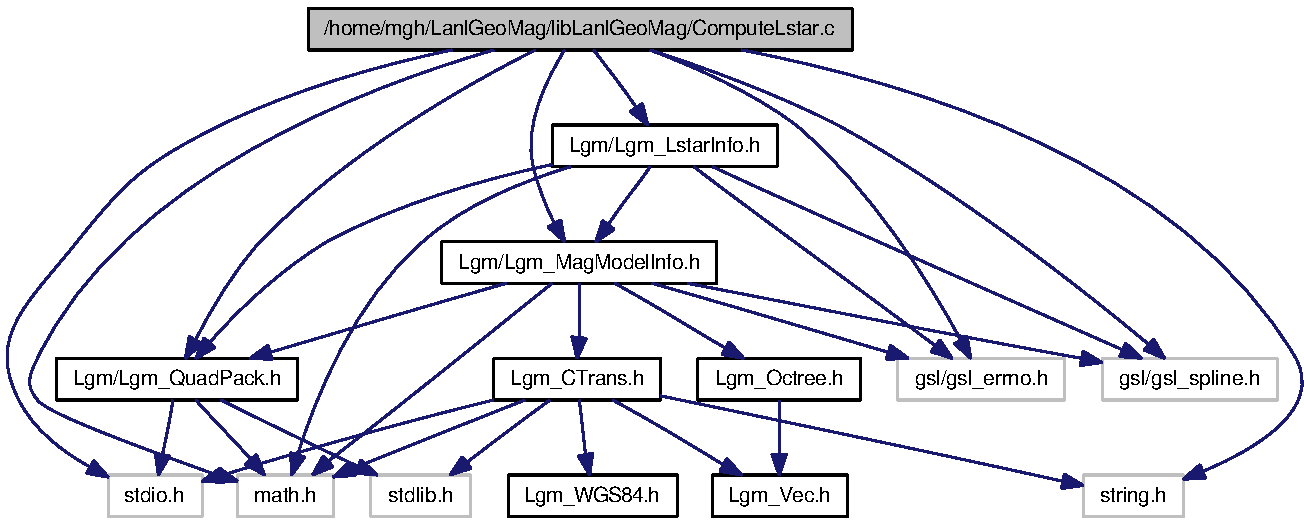
\includegraphics[width=331pt]{_compute_lstar_8c__incl}
\end{center}
\end{figure}
\subsection*{Defines}
\begin{CompactItemize}
\item 
\#define \hyperlink{_compute_lstar_8c_792d250cb395f0b2a568f17662b50b30}{DeltaMLT}~1.0
\end{CompactItemize}
\subsection*{Functions}
\begin{CompactItemize}
\item 
void \hyperlink{_compute_lstar_8c_6b9a47796fc6ddf11d42d91a9885e771}{PredictMlat1} (double $\ast$MirrorMLT, double $\ast$MirrorMlat, int k, double MLT, double $\ast$pred\_\-mlat, double $\ast$pred\_\-delta\_\-mlat, double $\ast$delta)
\item 
void \hyperlink{_compute_lstar_8c_7aae1b668ec7bda0f93ead3c5ecd5429}{PredictMlat2} (double $\ast$MirrorMLT, double $\ast$MirrorMlat, int k, double MLT, double $\ast$pred\_\-mlat, double $\ast$pred\_\-delta\_\-mlat, double $\ast$delta, \hyperlink{struct_lgm___lstar_info}{Lgm\_\-LstarInfo} $\ast$LstarInfo)
\item 
void \hyperlink{_compute_lstar_8c_fbfbd938470e255f3267132c6f96bc48}{SetLstarTolerances} (int Quality, \hyperlink{struct_lgm___lstar_info}{Lgm\_\-LstarInfo} $\ast$s)
\item 
\hyperlink{struct_lgm___lstar_info}{Lgm\_\-LstarInfo} $\ast$ \hyperlink{_compute_lstar_8c_d7d999fbe5d3b065fe808bb3e7ceab0b}{InitLstarInfo} (int VerbosityLevel)
\item 
void \hyperlink{_compute_lstar_8c_a7343c731e76ee9f5190b30a318656f6}{FreeLstarInfo} (\hyperlink{struct_lgm___lstar_info}{Lgm\_\-LstarInfo} $\ast$s)
\item 
\hyperlink{struct_lgm___lstar_info}{Lgm\_\-LstarInfo} $\ast$ \hyperlink{_compute_lstar_8c_84a1ec912704573c21c1e506b72d6f01}{Lgm\_\-CopyLstarInfo} (\hyperlink{struct_lgm___lstar_info}{Lgm\_\-LstarInfo} $\ast$s)
\item 
void \hyperlink{_compute_lstar_8c_68ec464c1b33f0b437d856629f0dd901}{NewTimeLstarInfo} (long int Date, double UT, double PitchAngle, int($\ast$Mag)(\hyperlink{struct_lgm___vector}{Lgm\_\-Vector} $\ast$, \hyperlink{struct_lgm___vector}{Lgm\_\-Vector} $\ast$, \hyperlink{struct_lgm___mag_model_info}{Lgm\_\-MagModelInfo} $\ast$), \hyperlink{struct_lgm___lstar_info}{Lgm\_\-LstarInfo} $\ast$LstarInfo)
\item 
int \hyperlink{_compute_lstar_8c_957a4d60eb4025656b3c2557b402523e}{Lstar} (\hyperlink{struct_lgm___vector}{Lgm\_\-Vector} $\ast$vin, \hyperlink{struct_lgm___lstar_info}{Lgm\_\-LstarInfo} $\ast$LstarInfo)
\item 
double \hyperlink{_compute_lstar_8c_5f75b0909329fb6260c63bc551c29acb}{MagFluxIntegrand} (double Phi, \hyperlink{_lgm___quad_pack_8h_01be5a7db8d2fc2ba26ce793d73b6472}{\_\-qpInfo} $\ast$qpInfo)
\item 
double \hyperlink{_compute_lstar_8c_871565dbd20b1df061fb2e706bd724db}{MagFlux} (\hyperlink{struct_lgm___lstar_info}{Lgm\_\-LstarInfo} $\ast$LstarInfo)
\item 
double \hyperlink{_compute_lstar_8c_fb4cfc3e9728d5ec4867d39f1384dc38}{LambdaIntegrand} (double Lambda, \hyperlink{_lgm___quad_pack_8h_01be5a7db8d2fc2ba26ce793d73b6472}{\_\-qpInfo} $\ast$qpInfo)
\item 
double \hyperlink{_compute_lstar_8c_593bd0ac5cd8b137cbc401b58219df31}{LambdaIntegral} (\hyperlink{struct_lgm___lstar_info}{Lgm\_\-LstarInfo} $\ast$LstarInfo)
\item 
double \hyperlink{_compute_lstar_8c_0f767b7206b1928b2f36fa7c5a26ca33}{MagFluxIntegrand2} (double Phi, \hyperlink{_lgm___quad_pack_8h_01be5a7db8d2fc2ba26ce793d73b6472}{\_\-qpInfo} $\ast$qpInfo)
\item 
double \hyperlink{_compute_lstar_8c_7da6f58b128b4aef809400ada95767d4}{MagFlux2} (\hyperlink{struct_lgm___lstar_info}{Lgm\_\-LstarInfo} $\ast$LstarInfo)
\end{CompactItemize}


\subsection{Define Documentation}
\hypertarget{_compute_lstar_8c_792d250cb395f0b2a568f17662b50b30}{
\index{ComputeLstar.c@{ComputeLstar.c}!DeltaMLT@{DeltaMLT}}
\index{DeltaMLT@{DeltaMLT}!ComputeLstar.c@{ComputeLstar.c}}
\subsubsection[{DeltaMLT}]{\setlength{\rightskip}{0pt plus 5cm}\#define DeltaMLT~1.0}}
\label{_compute_lstar_8c_792d250cb395f0b2a568f17662b50b30}




Definition at line 10 of file ComputeLstar.c.

\subsection{Function Documentation}
\hypertarget{_compute_lstar_8c_6b9a47796fc6ddf11d42d91a9885e771}{
\index{ComputeLstar.c@{ComputeLstar.c}!PredictMlat1@{PredictMlat1}}
\index{PredictMlat1@{PredictMlat1}!ComputeLstar.c@{ComputeLstar.c}}
\subsubsection[{PredictMlat1}]{\setlength{\rightskip}{0pt plus 5cm}void PredictMlat1 (double $\ast$ {\em MirrorMLT}, \/  double $\ast$ {\em MirrorMlat}, \/  int {\em k}, \/  double {\em MLT}, \/  double $\ast$ {\em pred\_\-mlat}, \/  double $\ast$ {\em pred\_\-delta\_\-mlat}, \/  double $\ast$ {\em delta})}}
\label{_compute_lstar_8c_6b9a47796fc6ddf11d42d91a9885e771}




Definition at line 1072 of file ComputeLstar.c.

Here is the call graph for this function:\nopagebreak
\begin{figure}[H]
\begin{center}
\leavevmode
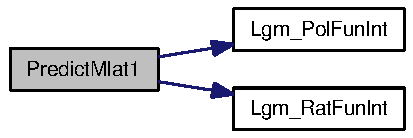
\includegraphics[width=117pt]{_compute_lstar_8c_6b9a47796fc6ddf11d42d91a9885e771_cgraph}
\end{center}
\end{figure}


Here is the caller graph for this function:\nopagebreak
\begin{figure}[H]
\begin{center}
\leavevmode
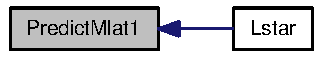
\includegraphics[width=95pt]{_compute_lstar_8c_6b9a47796fc6ddf11d42d91a9885e771_icgraph}
\end{center}
\end{figure}
\hypertarget{_compute_lstar_8c_7aae1b668ec7bda0f93ead3c5ecd5429}{
\index{ComputeLstar.c@{ComputeLstar.c}!PredictMlat2@{PredictMlat2}}
\index{PredictMlat2@{PredictMlat2}!ComputeLstar.c@{ComputeLstar.c}}
\subsubsection[{PredictMlat2}]{\setlength{\rightskip}{0pt plus 5cm}void PredictMlat2 (double $\ast$ {\em MirrorMLT}, \/  double $\ast$ {\em MirrorMlat}, \/  int {\em k}, \/  double {\em MLT}, \/  double $\ast$ {\em pred\_\-mlat}, \/  double $\ast$ {\em pred\_\-delta\_\-mlat}, \/  double $\ast$ {\em delta}, \/  {\bf Lgm\_\-LstarInfo} $\ast$ {\em LstarInfo})}}
\label{_compute_lstar_8c_7aae1b668ec7bda0f93ead3c5ecd5429}




Definition at line 1151 of file ComputeLstar.c.

Here is the call graph for this function:\nopagebreak
\begin{figure}[H]
\begin{center}
\leavevmode
\includegraphics[width=107pt]{_compute_lstar_8c_7aae1b668ec7bda0f93ead3c5ecd5429_cgraph}
\end{center}
\end{figure}


Here is the caller graph for this function:\nopagebreak
\begin{figure}[H]
\begin{center}
\leavevmode
\includegraphics[width=95pt]{_compute_lstar_8c_7aae1b668ec7bda0f93ead3c5ecd5429_icgraph}
\end{center}
\end{figure}
\hypertarget{_compute_lstar_8c_fbfbd938470e255f3267132c6f96bc48}{
\index{ComputeLstar.c@{ComputeLstar.c}!SetLstarTolerances@{SetLstarTolerances}}
\index{SetLstarTolerances@{SetLstarTolerances}!ComputeLstar.c@{ComputeLstar.c}}
\subsubsection[{SetLstarTolerances}]{\setlength{\rightskip}{0pt plus 5cm}void SetLstarTolerances (int {\em Quality}, \/  {\bf Lgm\_\-LstarInfo} $\ast$ {\em s})}}
\label{_compute_lstar_8c_fbfbd938470e255f3267132c6f96bc48}




Definition at line 21 of file ComputeLstar.c.\hypertarget{_compute_lstar_8c_d7d999fbe5d3b065fe808bb3e7ceab0b}{
\index{ComputeLstar.c@{ComputeLstar.c}!InitLstarInfo@{InitLstarInfo}}
\index{InitLstarInfo@{InitLstarInfo}!ComputeLstar.c@{ComputeLstar.c}}
\subsubsection[{InitLstarInfo}]{\setlength{\rightskip}{0pt plus 5cm}{\bf Lgm\_\-LstarInfo}$\ast$ InitLstarInfo (int {\em VerbosityLevel})}}
\label{_compute_lstar_8c_d7d999fbe5d3b065fe808bb3e7ceab0b}




Definition at line 189 of file ComputeLstar.c.

Here is the call graph for this function:\nopagebreak
\begin{figure}[H]
\begin{center}
\leavevmode
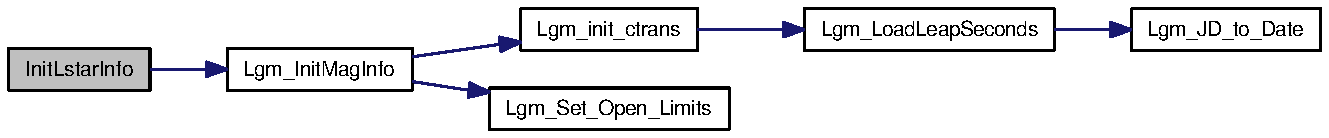
\includegraphics[width=337pt]{_compute_lstar_8c_d7d999fbe5d3b065fe808bb3e7ceab0b_cgraph}
\end{center}
\end{figure}


Here is the caller graph for this function:\nopagebreak
\begin{figure}[H]
\begin{center}
\leavevmode
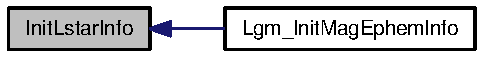
\includegraphics[width=134pt]{_compute_lstar_8c_d7d999fbe5d3b065fe808bb3e7ceab0b_icgraph}
\end{center}
\end{figure}
\hypertarget{_compute_lstar_8c_a7343c731e76ee9f5190b30a318656f6}{
\index{ComputeLstar.c@{ComputeLstar.c}!FreeLstarInfo@{FreeLstarInfo}}
\index{FreeLstarInfo@{FreeLstarInfo}!ComputeLstar.c@{ComputeLstar.c}}
\subsubsection[{FreeLstarInfo}]{\setlength{\rightskip}{0pt plus 5cm}void FreeLstarInfo ({\bf Lgm\_\-LstarInfo} $\ast$ {\em s})}}
\label{_compute_lstar_8c_a7343c731e76ee9f5190b30a318656f6}




Definition at line 221 of file ComputeLstar.c.

Here is the call graph for this function:\nopagebreak
\begin{figure}[H]
\begin{center}
\leavevmode
\includegraphics[width=188pt]{_compute_lstar_8c_a7343c731e76ee9f5190b30a318656f6_cgraph}
\end{center}
\end{figure}


Here is the caller graph for this function:\nopagebreak
\begin{figure}[H]
\begin{center}
\leavevmode
\includegraphics[width=140pt]{_compute_lstar_8c_a7343c731e76ee9f5190b30a318656f6_icgraph}
\end{center}
\end{figure}
\hypertarget{_compute_lstar_8c_84a1ec912704573c21c1e506b72d6f01}{
\index{ComputeLstar.c@{ComputeLstar.c}!Lgm\_\-CopyLstarInfo@{Lgm\_\-CopyLstarInfo}}
\index{Lgm\_\-CopyLstarInfo@{Lgm\_\-CopyLstarInfo}!ComputeLstar.c@{ComputeLstar.c}}
\subsubsection[{Lgm\_\-CopyLstarInfo}]{\setlength{\rightskip}{0pt plus 5cm}{\bf Lgm\_\-LstarInfo}$\ast$ Lgm\_\-CopyLstarInfo ({\bf Lgm\_\-LstarInfo} $\ast$ {\em s})}}
\label{_compute_lstar_8c_84a1ec912704573c21c1e506b72d6f01}




Definition at line 235 of file ComputeLstar.c.

Here is the call graph for this function:\nopagebreak
\begin{figure}[H]
\begin{center}
\leavevmode
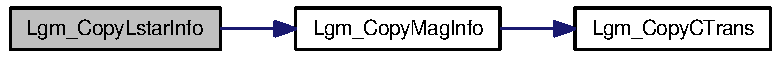
\includegraphics[width=205pt]{_compute_lstar_8c_84a1ec912704573c21c1e506b72d6f01_cgraph}
\end{center}
\end{figure}
\hypertarget{_compute_lstar_8c_68ec464c1b33f0b437d856629f0dd901}{
\index{ComputeLstar.c@{ComputeLstar.c}!NewTimeLstarInfo@{NewTimeLstarInfo}}
\index{NewTimeLstarInfo@{NewTimeLstarInfo}!ComputeLstar.c@{ComputeLstar.c}}
\subsubsection[{NewTimeLstarInfo}]{\setlength{\rightskip}{0pt plus 5cm}void NewTimeLstarInfo (long int {\em Date}, \/  double {\em UT}, \/  double {\em PitchAngle}, \/  int($\ast$)({\bf Lgm\_\-Vector} $\ast$, {\bf Lgm\_\-Vector} $\ast$, {\bf Lgm\_\-MagModelInfo} $\ast$) {\em Mag}, \/  {\bf Lgm\_\-LstarInfo} $\ast$ {\em LstarInfo})}}
\label{_compute_lstar_8c_68ec464c1b33f0b437d856629f0dd901}




Definition at line 281 of file ComputeLstar.c.

Here is the call graph for this function:\nopagebreak
\begin{figure}[H]
\begin{center}
\leavevmode
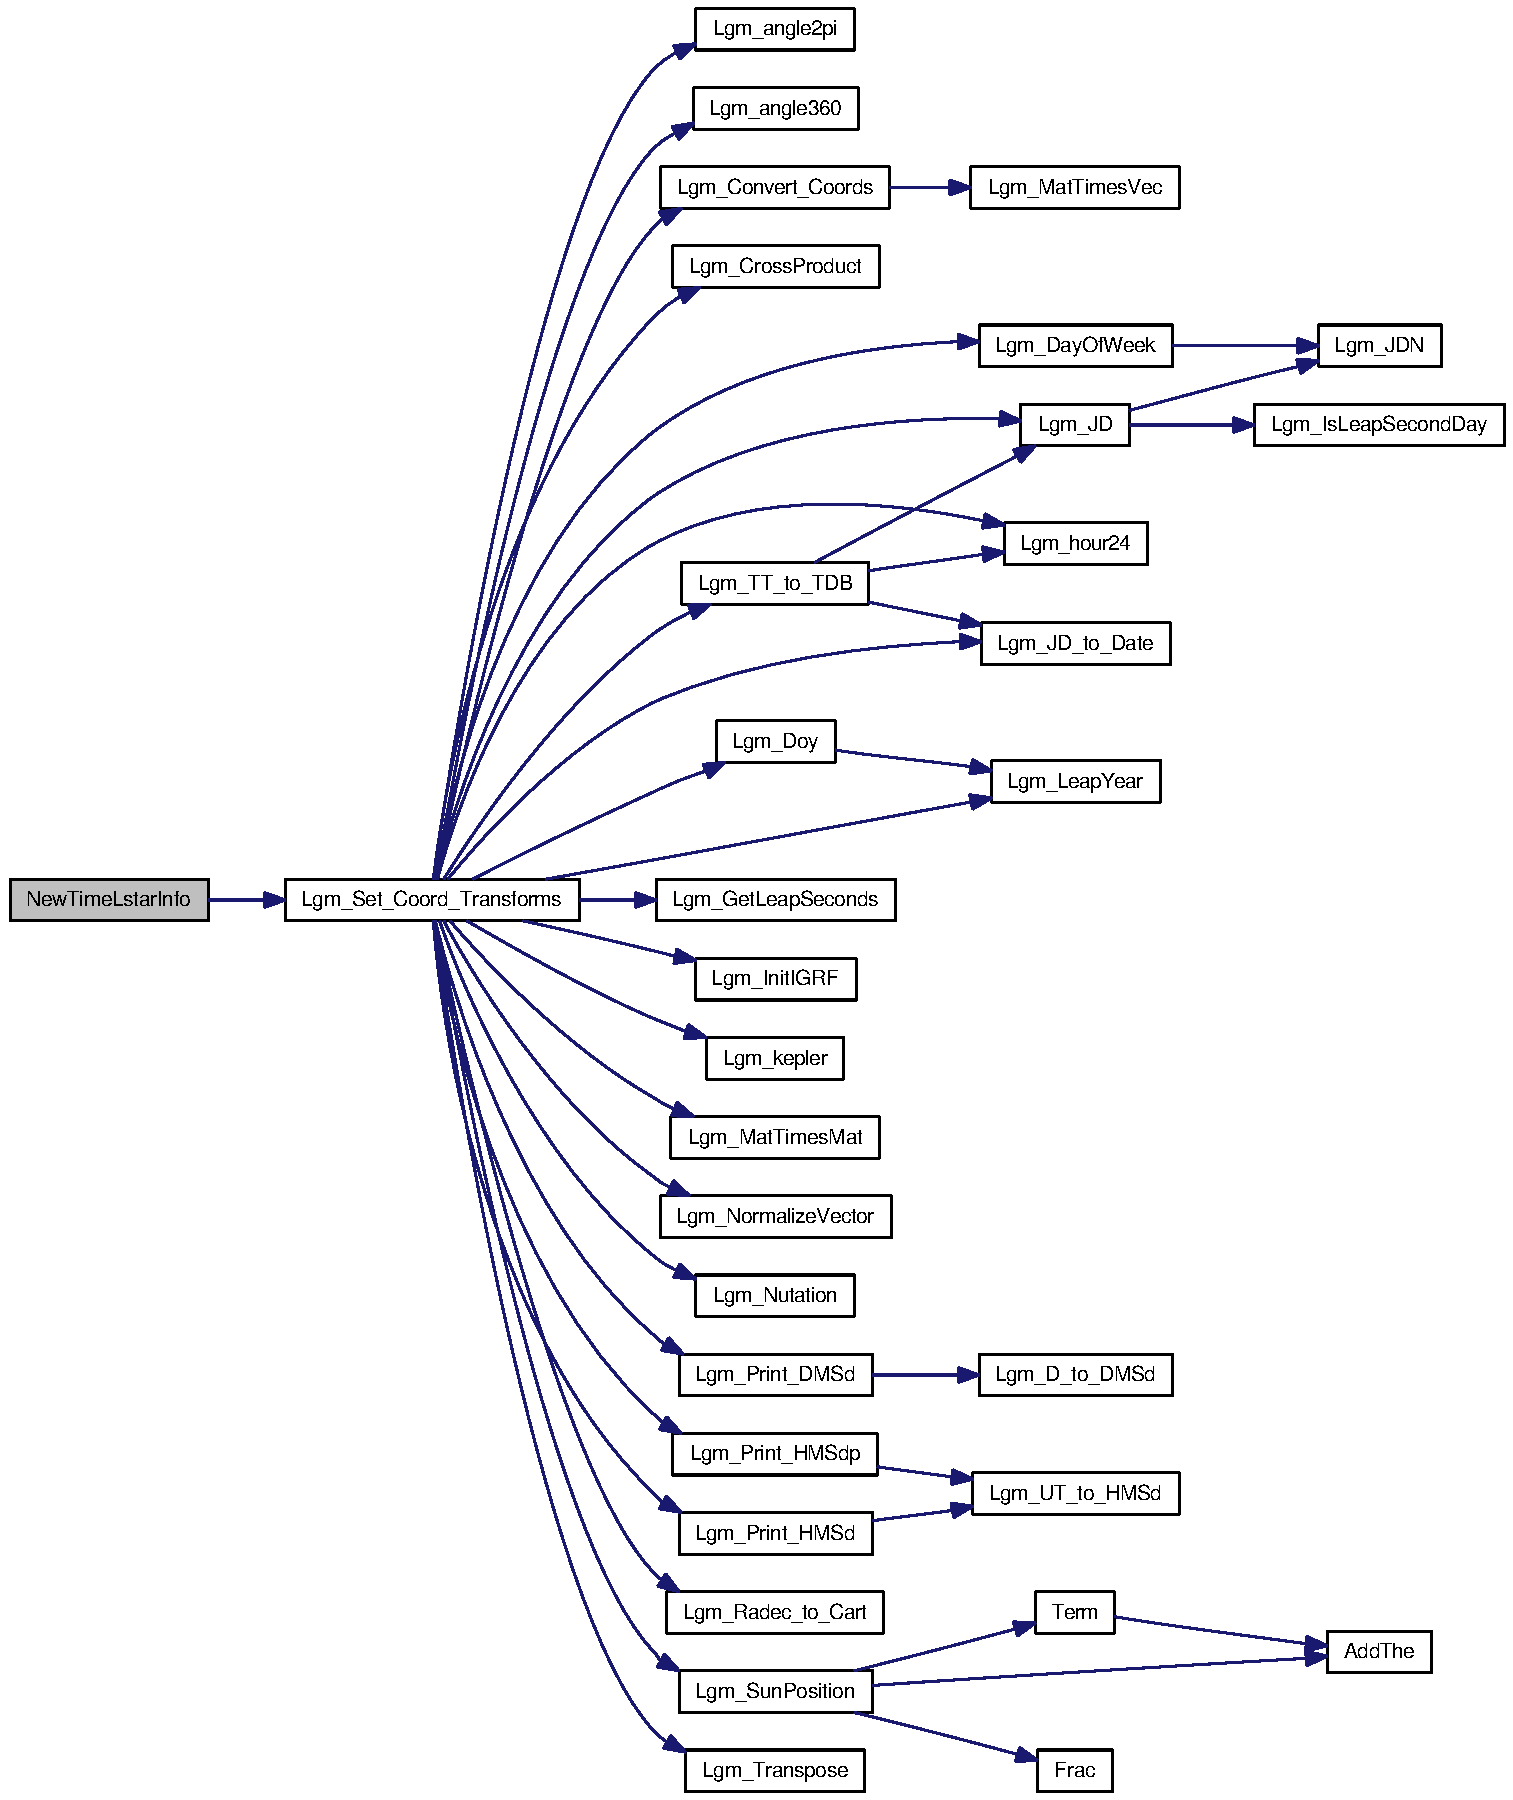
\includegraphics[width=381pt]{_compute_lstar_8c_68ec464c1b33f0b437d856629f0dd901_cgraph}
\end{center}
\end{figure}
\hypertarget{_compute_lstar_8c_957a4d60eb4025656b3c2557b402523e}{
\index{ComputeLstar.c@{ComputeLstar.c}!Lstar@{Lstar}}
\index{Lstar@{Lstar}!ComputeLstar.c@{ComputeLstar.c}}
\subsubsection[{Lstar}]{\setlength{\rightskip}{0pt plus 5cm}int Lstar ({\bf Lgm\_\-Vector} $\ast$ {\em vin}, \/  {\bf Lgm\_\-LstarInfo} $\ast$ {\em LstarInfo})}}
\label{_compute_lstar_8c_957a4d60eb4025656b3c2557b402523e}




Definition at line 307 of file ComputeLstar.c.

Here is the call graph for this function:\nopagebreak
\begin{figure}[H]
\begin{center}
\leavevmode
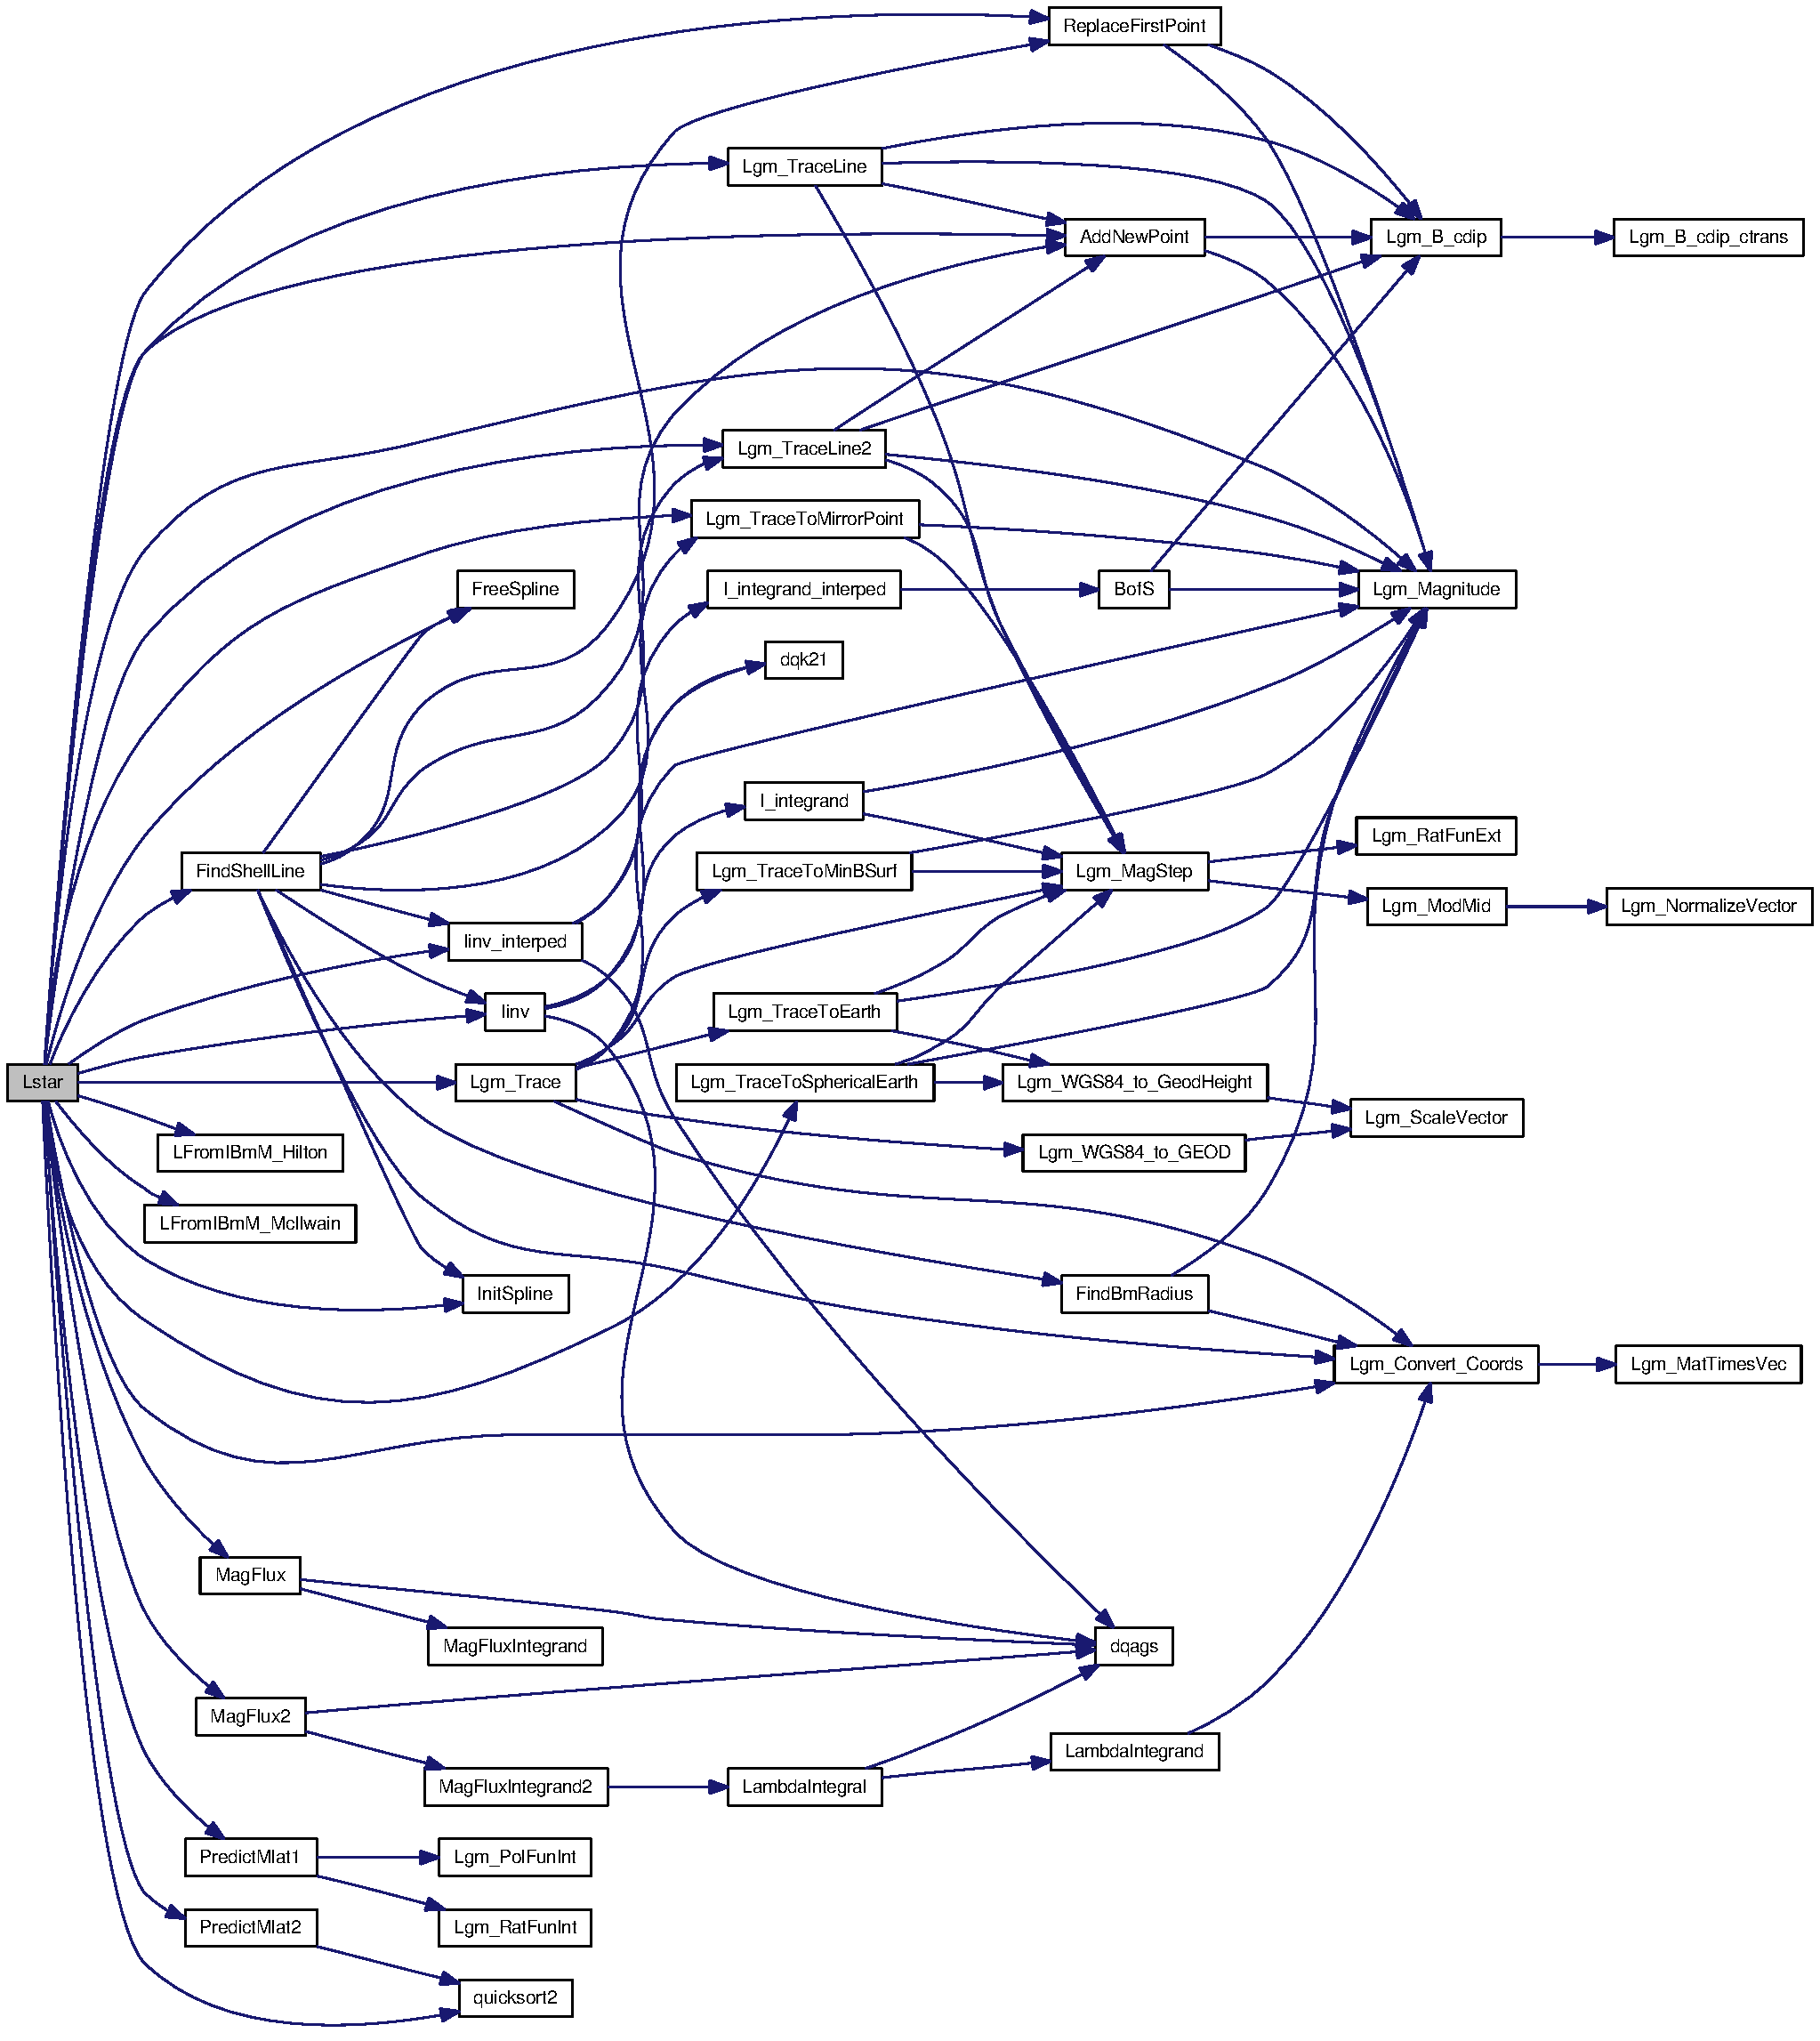
\includegraphics[width=420pt]{_compute_lstar_8c_957a4d60eb4025656b3c2557b402523e_cgraph}
\end{center}
\end{figure}
\hypertarget{_compute_lstar_8c_5f75b0909329fb6260c63bc551c29acb}{
\index{ComputeLstar.c@{ComputeLstar.c}!MagFluxIntegrand@{MagFluxIntegrand}}
\index{MagFluxIntegrand@{MagFluxIntegrand}!ComputeLstar.c@{ComputeLstar.c}}
\subsubsection[{MagFluxIntegrand}]{\setlength{\rightskip}{0pt plus 5cm}double MagFluxIntegrand (double {\em Phi}, \/  {\bf \_\-qpInfo} $\ast$ {\em qpInfo})}}
\label{_compute_lstar_8c_5f75b0909329fb6260c63bc551c29acb}




Definition at line 815 of file ComputeLstar.c.

Here is the caller graph for this function:\nopagebreak
\begin{figure}[H]
\begin{center}
\leavevmode
\includegraphics[width=151pt]{_compute_lstar_8c_5f75b0909329fb6260c63bc551c29acb_icgraph}
\end{center}
\end{figure}
\hypertarget{_compute_lstar_8c_871565dbd20b1df061fb2e706bd724db}{
\index{ComputeLstar.c@{ComputeLstar.c}!MagFlux@{MagFlux}}
\index{MagFlux@{MagFlux}!ComputeLstar.c@{ComputeLstar.c}}
\subsubsection[{MagFlux}]{\setlength{\rightskip}{0pt plus 5cm}double MagFlux ({\bf Lgm\_\-LstarInfo} $\ast$ {\em LstarInfo})}}
\label{_compute_lstar_8c_871565dbd20b1df061fb2e706bd724db}




Definition at line 842 of file ComputeLstar.c.

Here is the call graph for this function:\nopagebreak
\begin{figure}[H]
\begin{center}
\leavevmode
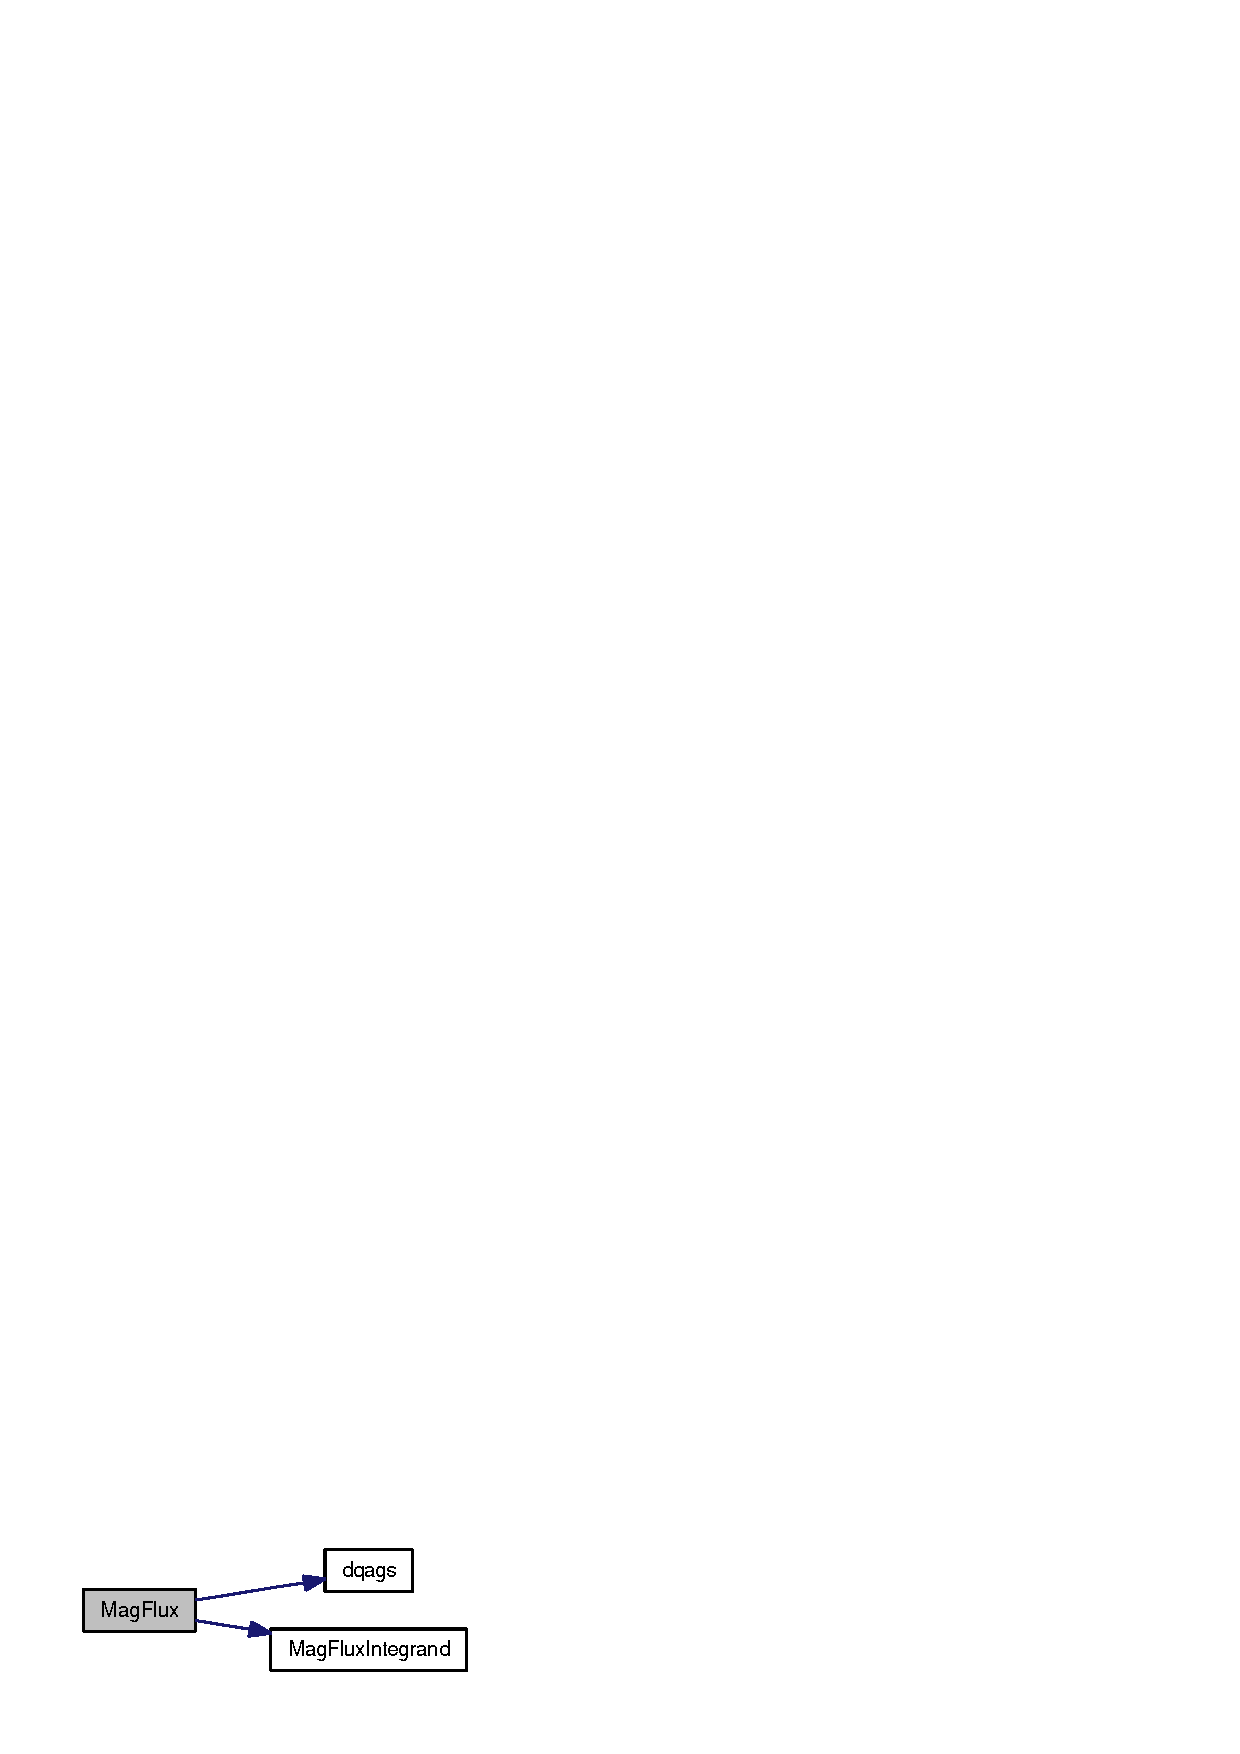
\includegraphics[width=114pt]{_compute_lstar_8c_871565dbd20b1df061fb2e706bd724db_cgraph}
\end{center}
\end{figure}


Here is the caller graph for this function:\nopagebreak
\begin{figure}[H]
\begin{center}
\leavevmode
\includegraphics[width=86pt]{_compute_lstar_8c_871565dbd20b1df061fb2e706bd724db_icgraph}
\end{center}
\end{figure}
\hypertarget{_compute_lstar_8c_fb4cfc3e9728d5ec4867d39f1384dc38}{
\index{ComputeLstar.c@{ComputeLstar.c}!LambdaIntegrand@{LambdaIntegrand}}
\index{LambdaIntegrand@{LambdaIntegrand}!ComputeLstar.c@{ComputeLstar.c}}
\subsubsection[{LambdaIntegrand}]{\setlength{\rightskip}{0pt plus 5cm}double LambdaIntegrand (double {\em Lambda}, \/  {\bf \_\-qpInfo} $\ast$ {\em qpInfo})}}
\label{_compute_lstar_8c_fb4cfc3e9728d5ec4867d39f1384dc38}




Definition at line 909 of file ComputeLstar.c.

Here is the call graph for this function:\nopagebreak
\begin{figure}[H]
\begin{center}
\leavevmode
\includegraphics[width=209pt]{_compute_lstar_8c_fb4cfc3e9728d5ec4867d39f1384dc38_cgraph}
\end{center}
\end{figure}


Here is the caller graph for this function:\nopagebreak
\begin{figure}[H]
\begin{center}
\leavevmode
\includegraphics[width=281pt]{_compute_lstar_8c_fb4cfc3e9728d5ec4867d39f1384dc38_icgraph}
\end{center}
\end{figure}
\hypertarget{_compute_lstar_8c_593bd0ac5cd8b137cbc401b58219df31}{
\index{ComputeLstar.c@{ComputeLstar.c}!LambdaIntegral@{LambdaIntegral}}
\index{LambdaIntegral@{LambdaIntegral}!ComputeLstar.c@{ComputeLstar.c}}
\subsubsection[{LambdaIntegral}]{\setlength{\rightskip}{0pt plus 5cm}double LambdaIntegral ({\bf Lgm\_\-LstarInfo} $\ast$ {\em LstarInfo})}}
\label{_compute_lstar_8c_593bd0ac5cd8b137cbc401b58219df31}




Definition at line 945 of file ComputeLstar.c.

Here is the call graph for this function:\nopagebreak
\begin{figure}[H]
\begin{center}
\leavevmode
\includegraphics[width=269pt]{_compute_lstar_8c_593bd0ac5cd8b137cbc401b58219df31_cgraph}
\end{center}
\end{figure}


Here is the caller graph for this function:\nopagebreak
\begin{figure}[H]
\begin{center}
\leavevmode
\includegraphics[width=217pt]{_compute_lstar_8c_593bd0ac5cd8b137cbc401b58219df31_icgraph}
\end{center}
\end{figure}
\hypertarget{_compute_lstar_8c_0f767b7206b1928b2f36fa7c5a26ca33}{
\index{ComputeLstar.c@{ComputeLstar.c}!MagFluxIntegrand2@{MagFluxIntegrand2}}
\index{MagFluxIntegrand2@{MagFluxIntegrand2}!ComputeLstar.c@{ComputeLstar.c}}
\subsubsection[{MagFluxIntegrand2}]{\setlength{\rightskip}{0pt plus 5cm}double MagFluxIntegrand2 (double {\em Phi}, \/  {\bf \_\-qpInfo} $\ast$ {\em qpInfo})}}
\label{_compute_lstar_8c_0f767b7206b1928b2f36fa7c5a26ca33}




Definition at line 1005 of file ComputeLstar.c.

Here is the call graph for this function:\nopagebreak
\begin{figure}[H]
\begin{center}
\leavevmode
\includegraphics[width=337pt]{_compute_lstar_8c_0f767b7206b1928b2f36fa7c5a26ca33_cgraph}
\end{center}
\end{figure}


Here is the caller graph for this function:\nopagebreak
\begin{figure}[H]
\begin{center}
\leavevmode
\includegraphics[width=157pt]{_compute_lstar_8c_0f767b7206b1928b2f36fa7c5a26ca33_icgraph}
\end{center}
\end{figure}
\hypertarget{_compute_lstar_8c_7da6f58b128b4aef809400ada95767d4}{
\index{ComputeLstar.c@{ComputeLstar.c}!MagFlux2@{MagFlux2}}
\index{MagFlux2@{MagFlux2}!ComputeLstar.c@{ComputeLstar.c}}
\subsubsection[{MagFlux2}]{\setlength{\rightskip}{0pt plus 5cm}double MagFlux2 ({\bf Lgm\_\-LstarInfo} $\ast$ {\em LstarInfo})}}
\label{_compute_lstar_8c_7da6f58b128b4aef809400ada95767d4}




Definition at line 1023 of file ComputeLstar.c.

Here is the call graph for this function:\nopagebreak
\begin{figure}[H]
\begin{center}
\leavevmode
\includegraphics[width=385pt]{_compute_lstar_8c_7da6f58b128b4aef809400ada95767d4_cgraph}
\end{center}
\end{figure}


Here is the caller graph for this function:\nopagebreak
\begin{figure}[H]
\begin{center}
\leavevmode
\includegraphics[width=89pt]{_compute_lstar_8c_7da6f58b128b4aef809400ada95767d4_icgraph}
\end{center}
\end{figure}

\hypertarget{dqagi_8f}{
\section{/home/mgh/LanlGeoMag/libLanlGeoMag/dqagi.f File Reference}
\label{dqagi_8f}\index{/home/mgh/LanlGeoMag/libLanlGeoMag/dqagi.f@{/home/mgh/LanlGeoMag/libLanlGeoMag/dqagi.f}}
}
\subsection*{Functions}
\begin{CompactItemize}
\item 
subroutine \hyperlink{dqagi_8f_26b0258ec25eb3725ba606146dc6c364}{DQAGI} (F, BOUND, INF, EPSABS, EPSREL, RESULT, ABSERR, NEVAL, IER, LIMIT, LENW, LAST, IWORK, WORK)
\end{CompactItemize}


\subsection{Function Documentation}
\hypertarget{dqagi_8f_26b0258ec25eb3725ba606146dc6c364}{
\index{dqagi.f@{dqagi.f}!DQAGI@{DQAGI}}
\index{DQAGI@{DQAGI}!dqagi.f@{dqagi.f}}
\subsubsection[{DQAGI}]{\setlength{\rightskip}{0pt plus 5cm}subroutine DQAGI (DOUBLE PRECISION,external {\em F}, \/  DOUBLE PRECISION {\em BOUND}, \/  INTEGER {\em INF}, \/  DOUBLE PRECISION {\em EPSABS}, \/  DOUBLE PRECISION {\em EPSREL}, \/  DOUBLE PRECISION {\em RESULT}, \/  DOUBLE PRECISION {\em ABSERR}, \/  INTEGER {\em NEVAL}, \/  INTEGER {\em IER}, \/  INTEGER {\em LIMIT}, \/  INTEGER {\em LENW}, \/  INTEGER {\em LAST}, \/  INTEGER,dimension($\ast$),dimension {\em IWORK}, \/  DOUBLE PRECISION,dimension($\ast$),dimension {\em WORK})}}
\label{dqagi_8f_26b0258ec25eb3725ba606146dc6c364}




Definition at line 2 of file dqagi.f.

Here is the call graph for this function:\nopagebreak
\begin{figure}[H]
\begin{center}
\leavevmode
\includegraphics[width=91pt]{dqagi_8f_26b0258ec25eb3725ba606146dc6c364_cgraph}
\end{center}
\end{figure}

\hypertarget{dqagie_8f}{
\section{/home/mgh/LanlGeoMag/libLanlGeoMag/dqagie.f File Reference}
\label{dqagie_8f}\index{/home/mgh/LanlGeoMag/libLanlGeoMag/dqagie.f@{/home/mgh/LanlGeoMag/libLanlGeoMag/dqagie.f}}
}
\subsection*{Functions}
\begin{CompactItemize}
\item 
subroutine \hyperlink{dqagie_8f_9224a43ef38ca8c3dfe37ad1646d9ab4}{DQAGIE} (F, BOUND, INF, EPSABS, EPSREL, LIMIT, RESULT, ABSERR, NEVAL, IER, ALIST, BLIST, RLIST, ELIST, IORD, LAST)
\end{CompactItemize}


\subsection{Function Documentation}
\hypertarget{dqagie_8f_9224a43ef38ca8c3dfe37ad1646d9ab4}{
\index{dqagie.f@{dqagie.f}!DQAGIE@{DQAGIE}}
\index{DQAGIE@{DQAGIE}!dqagie.f@{dqagie.f}}
\subsubsection[{DQAGIE}]{\setlength{\rightskip}{0pt plus 5cm}subroutine DQAGIE (DOUBLE PRECISION,external {\em F}, \/  DOUBLE PRECISION {\em BOUND}, \/  INTEGER {\em INF}, \/  DOUBLE PRECISION {\em EPSABS}, \/  DOUBLE PRECISION {\em EPSREL}, \/  INTEGER {\em LIMIT}, \/  DOUBLE PRECISION {\em RESULT}, \/  DOUBLE PRECISION {\em ABSERR}, \/  INTEGER {\em NEVAL}, \/  INTEGER {\em IER}, \/  DOUBLE PRECISION,dimension($\ast$),dimension {\em ALIST}, \/  DOUBLE PRECISION,dimension($\ast$),dimension {\em BLIST}, \/  DOUBLE PRECISION,dimension($\ast$),dimension {\em RLIST}, \/  DOUBLE PRECISION,dimension($\ast$),dimension {\em ELIST}, \/  INTEGER,dimension($\ast$),dimension {\em IORD}, \/  INTEGER {\em LAST})}}
\label{dqagie_8f_9224a43ef38ca8c3dfe37ad1646d9ab4}




Definition at line 2 of file dqagie.f.

Here is the caller graph for this function:\nopagebreak
\begin{figure}[H]
\begin{center}
\leavevmode
\includegraphics[width=91pt]{dqagie_8f_9224a43ef38ca8c3dfe37ad1646d9ab4_icgraph}
\end{center}
\end{figure}

\hypertarget{dqagp_8f}{
\section{/home/mgh/LanlGeoMag/libLanlGeoMag/dqagp.f File Reference}
\label{dqagp_8f}\index{/home/mgh/LanlGeoMag/libLanlGeoMag/dqagp.f@{/home/mgh/LanlGeoMag/libLanlGeoMag/dqagp.f}}
}
\subsection*{Functions}
\begin{CompactItemize}
\item 
subroutine \hyperlink{dqagp_8f_3809d8d2a43b03d1f3c0f7833c0d82c8}{DQAGP} (F, A, B, NPTS2, POINTS, EPSABS, EPSREL, RESULT, ABSERR, NEVAL, IER, LENIW, LENW, LAST, IWORK, WORK)
\end{CompactItemize}


\subsection{Function Documentation}
\hypertarget{dqagp_8f_3809d8d2a43b03d1f3c0f7833c0d82c8}{
\index{dqagp.f@{dqagp.f}!DQAGP@{DQAGP}}
\index{DQAGP@{DQAGP}!dqagp.f@{dqagp.f}}
\subsubsection[{DQAGP}]{\setlength{\rightskip}{0pt plus 5cm}subroutine DQAGP (DOUBLE PRECISION,external {\em F}, \/  DOUBLE PRECISION {\em A}, \/  DOUBLE PRECISION {\em B}, \/  INTEGER {\em NPTS2}, \/  DOUBLE PRECISION,dimension($\ast$),dimension {\em POINTS}, \/  DOUBLE PRECISION {\em EPSABS}, \/  DOUBLE PRECISION {\em EPSREL}, \/  DOUBLE PRECISION {\em RESULT}, \/  DOUBLE PRECISION {\em ABSERR}, \/  INTEGER {\em NEVAL}, \/  INTEGER {\em IER}, \/  INTEGER {\em LENIW}, \/  INTEGER {\em LENW}, \/  INTEGER {\em LAST}, \/  INTEGER,dimension($\ast$),dimension {\em IWORK}, \/  DOUBLE PRECISION,dimension($\ast$),dimension {\em WORK})}}
\label{dqagp_8f_3809d8d2a43b03d1f3c0f7833c0d82c8}




Definition at line 2 of file dqagp.f.

Here is the call graph for this function:\nopagebreak
\begin{figure}[H]
\begin{center}
\leavevmode
\includegraphics[width=95pt]{dqagp_8f_3809d8d2a43b03d1f3c0f7833c0d82c8_cgraph}
\end{center}
\end{figure}

\hypertarget{dqagpe_8f}{
\section{/home/mgh/LanlGeoMag/libLanlGeoMag/dqagpe.f File Reference}
\label{dqagpe_8f}\index{/home/mgh/LanlGeoMag/libLanlGeoMag/dqagpe.f@{/home/mgh/LanlGeoMag/libLanlGeoMag/dqagpe.f}}
}
\subsection*{Functions}
\begin{CompactItemize}
\item 
subroutine \hyperlink{dqagpe_8f_8e4f830cdfce930181f12c0775ecfc49}{DQAGPE} (F, A, B, NPTS2, POINTS, EPSABS, EPSREL, LIMIT, RESULT, ABSERR, NEVAL, IER, ALIST, BLIST, RLIST, ELIST, PTS, IORD, LEVEL, NDIN, LAST)
\end{CompactItemize}


\subsection{Function Documentation}
\hypertarget{dqagpe_8f_8e4f830cdfce930181f12c0775ecfc49}{
\index{dqagpe.f@{dqagpe.f}!DQAGPE@{DQAGPE}}
\index{DQAGPE@{DQAGPE}!dqagpe.f@{dqagpe.f}}
\subsubsection[{DQAGPE}]{\setlength{\rightskip}{0pt plus 5cm}subroutine DQAGPE (DOUBLE PRECISION,external {\em F}, \/  DOUBLE PRECISION {\em A}, \/  DOUBLE PRECISION {\em B}, \/  INTEGER {\em NPTS2}, \/  DOUBLE PRECISION,dimension($\ast$),dimension {\em POINTS}, \/  DOUBLE PRECISION {\em EPSABS}, \/  DOUBLE PRECISION {\em EPSREL}, \/  INTEGER {\em LIMIT}, \/  DOUBLE PRECISION {\em RESULT}, \/  DOUBLE PRECISION {\em ABSERR}, \/  INTEGER {\em NEVAL}, \/  INTEGER {\em IER}, \/  DOUBLE PRECISION,dimension($\ast$),dimension {\em ALIST}, \/  DOUBLE PRECISION,dimension($\ast$),dimension {\em BLIST}, \/  DOUBLE PRECISION,dimension($\ast$),dimension {\em RLIST}, \/  DOUBLE PRECISION,dimension($\ast$),dimension {\em ELIST}, \/  DOUBLE PRECISION,dimension($\ast$),dimension {\em PTS}, \/  INTEGER,dimension($\ast$),dimension {\em IORD}, \/  INTEGER,dimension($\ast$),dimension {\em LEVEL}, \/  INTEGER,dimension($\ast$),dimension {\em NDIN}, \/  INTEGER {\em LAST})}}
\label{dqagpe_8f_8e4f830cdfce930181f12c0775ecfc49}




Definition at line 2 of file dqagpe.f.

Here is the caller graph for this function:\nopagebreak
\begin{figure}[H]
\begin{center}
\leavevmode
\includegraphics[width=95pt]{dqagpe_8f_8e4f830cdfce930181f12c0775ecfc49_icgraph}
\end{center}
\end{figure}

\hypertarget{_drift_shell_8c}{
\section{/home/mgh/LanlGeoMag/libLanlGeoMag/DriftShell.c File Reference}
\label{_drift_shell_8c}\index{/home/mgh/LanlGeoMag/libLanlGeoMag/DriftShell.c@{/home/mgh/LanlGeoMag/libLanlGeoMag/DriftShell.c}}
}
{\tt \#include \char`\"{}Lgm/Lgm\_\-MagModelInfo.h\char`\"{}}\par
{\tt \#include \char`\"{}Lgm/Lgm\_\-LstarInfo.h\char`\"{}}\par


Include dependency graph for DriftShell.c:\nopagebreak
\begin{figure}[H]
\begin{center}
\leavevmode
\includegraphics[width=326pt]{_drift_shell_8c__incl}
\end{center}
\end{figure}
\subsection*{Functions}
\begin{CompactItemize}
\item 
int \hyperlink{_drift_shell_8c_e79603e88bcb7860ca33e8fe4fbdf37f}{FindShellLine} (double I0, double $\ast$Ifound, double Bm, double MLT, double $\ast$mlat, double $\ast$rad, double mlat0, double mlat1, \hyperlink{struct_lgm___lstar_info}{Lgm\_\-LstarInfo} $\ast$LstarInfo)
\item 
int \hyperlink{_drift_shell_8c_15d887d6b99cb83ce58b5a04a171ec67}{FindBmRadius} (double Bm, double MLT, double mlat, double $\ast$r, double tol, \hyperlink{struct_lgm___lstar_info}{Lgm\_\-LstarInfo} $\ast$LstarInfo)
\end{CompactItemize}


\subsection{Function Documentation}
\hypertarget{_drift_shell_8c_e79603e88bcb7860ca33e8fe4fbdf37f}{
\index{DriftShell.c@{DriftShell.c}!FindShellLine@{FindShellLine}}
\index{FindShellLine@{FindShellLine}!DriftShell.c@{DriftShell.c}}
\subsubsection[{FindShellLine}]{\setlength{\rightskip}{0pt plus 5cm}int FindShellLine (double {\em I0}, \/  double $\ast$ {\em Ifound}, \/  double {\em Bm}, \/  double {\em MLT}, \/  double $\ast$ {\em mlat}, \/  double $\ast$ {\em rad}, \/  double {\em mlat0}, \/  double {\em mlat1}, \/  {\bf Lgm\_\-LstarInfo} $\ast$ {\em LstarInfo})}}
\label{_drift_shell_8c_e79603e88bcb7860ca33e8fe4fbdf37f}




Definition at line 36 of file DriftShell.c.

Here is the call graph for this function:\nopagebreak
\begin{figure}[H]
\begin{center}
\leavevmode
\includegraphics[width=401pt]{_drift_shell_8c_e79603e88bcb7860ca33e8fe4fbdf37f_cgraph}
\end{center}
\end{figure}


Here is the caller graph for this function:\nopagebreak
\begin{figure}[H]
\begin{center}
\leavevmode
\includegraphics[width=97pt]{_drift_shell_8c_e79603e88bcb7860ca33e8fe4fbdf37f_icgraph}
\end{center}
\end{figure}
\hypertarget{_drift_shell_8c_15d887d6b99cb83ce58b5a04a171ec67}{
\index{DriftShell.c@{DriftShell.c}!FindBmRadius@{FindBmRadius}}
\index{FindBmRadius@{FindBmRadius}!DriftShell.c@{DriftShell.c}}
\subsubsection[{FindBmRadius}]{\setlength{\rightskip}{0pt plus 5cm}int FindBmRadius (double {\em Bm}, \/  double {\em MLT}, \/  double {\em mlat}, \/  double $\ast$ {\em r}, \/  double {\em tol}, \/  {\bf Lgm\_\-LstarInfo} $\ast$ {\em LstarInfo})}}
\label{_drift_shell_8c_15d887d6b99cb83ce58b5a04a171ec67}




Definition at line 344 of file DriftShell.c.

Here is the call graph for this function:\nopagebreak
\begin{figure}[H]
\begin{center}
\leavevmode
\includegraphics[width=203pt]{_drift_shell_8c_15d887d6b99cb83ce58b5a04a171ec67_cgraph}
\end{center}
\end{figure}


Here is the caller graph for this function:\nopagebreak
\begin{figure}[H]
\begin{center}
\leavevmode
\includegraphics[width=155pt]{_drift_shell_8c_15d887d6b99cb83ce58b5a04a171ec67_icgraph}
\end{center}
\end{figure}

\hypertarget{field__t96mod___m_g_h_8f}{
\section{/home/mgh/LanlGeoMag/libLanlGeoMag/field\_\-t96mod\_\-MGH.f File Reference}
\label{field__t96mod___m_g_h_8f}\index{/home/mgh/LanlGeoMag/libLanlGeoMag/field\_\-t96mod\_\-MGH.f@{/home/mgh/LanlGeoMag/libLanlGeoMag/field\_\-t96mod\_\-MGH.f}}
}
\subsection*{Functions}
\begin{CompactItemize}
\item 
subroutine \hyperlink{field__t96mod___m_g_h_8f_5a732b256b81c865c31b7f742ed6f797}{LGM\_\-FIELD\_\-T96MOD\_\-MGH} (PARMOD, AMDFIN, IYEAR, IDAY, IH, IM,$\ast$SEC, X, Y, Z, BX, BY, BZ)
\end{CompactItemize}


\subsection{Function Documentation}
\hypertarget{field__t96mod___m_g_h_8f_5a732b256b81c865c31b7f742ed6f797}{
\index{field\_\-t96mod\_\-MGH.f@{field\_\-t96mod\_\-MGH.f}!LGM\_\-FIELD\_\-T96MOD\_\-MGH@{LGM\_\-FIELD\_\-T96MOD\_\-MGH}}
\index{LGM\_\-FIELD\_\-T96MOD\_\-MGH@{LGM\_\-FIELD\_\-T96MOD\_\-MGH}!field_t96mod_MGH.f@{field\_\-t96mod\_\-MGH.f}}
\subsubsection[{LGM\_\-FIELD\_\-T96MOD\_\-MGH}]{\setlength{\rightskip}{0pt plus 5cm}subroutine LGM\_\-FIELD\_\-T96MOD\_\-MGH (REAL$\ast$8,dimension(10) {\em PARMOD}, \/  REAL$\ast$8,dimension(10) {\em AMDFIN}, \/  IYEAR, \/  IDAY, \/  IH, \/  IM, \/  $\ast$ {\em SEC}, \/  X, \/  Y, \/  Z, \/  BX, \/  BY, \/  BZ)}}
\label{field__t96mod___m_g_h_8f_5a732b256b81c865c31b7f742ed6f797}




Definition at line 1 of file field\_\-t96mod\_\-MGH.f.

Here is the call graph for this function:\nopagebreak
\begin{figure}[H]
\begin{center}
\leavevmode
\includegraphics[width=420pt]{field__t96mod___m_g_h_8f_5a732b256b81c865c31b7f742ed6f797_cgraph}
\end{center}
\end{figure}

\hypertarget{_geopack__2003_8f}{
\section{/home/mgh/LanlGeoMag/libLanlGeoMag/Geopack\_\-2003.f File Reference}
\label{_geopack__2003_8f}\index{/home/mgh/LanlGeoMag/libLanlGeoMag/Geopack\_\-2003.f@{/home/mgh/LanlGeoMag/libLanlGeoMag/Geopack\_\-2003.f}}
}
\subsection*{Functions}
\begin{CompactItemize}
\item 
subroutine \hyperlink{_geopack__2003_8f_7ed9719f68132703108e5b59d36d7c03}{IGRF\_\-GSM} (XGSM, YGSM, ZGSM, HXGSM, HYGSM, HZGSM)
\item 
subroutine \hyperlink{_geopack__2003_8f_d3225aa14c76ab4531fcf76deb3c15e0}{IGRF\_\-GEO} (R, THETA, PHI, BR, BTHETA, BPHI)
\item 
subroutine \hyperlink{_geopack__2003_8f_a4095b06f000636e34e2581a92ed28f0}{DIP} (XGSM, YGSM, ZGSM, BXGSM, BYGSM, BZGSM)
\item 
subroutine \hyperlink{_geopack__2003_8f_59da55e19c09037b70bd65ec97a3567a}{SUN} (IYEAR, IDAY, IHOUR, MINUTE, ISEC, GST, SLONG, SRASN, SDEC)
\item 
subroutine \hyperlink{_geopack__2003_8f_51cbeafec4591bc974f865375cec3975}{SPHCAR} (R, THETA, PHI, X, Y, Z, J)
\item 
subroutine \hyperlink{_geopack__2003_8f_39f847a454b8691795bb0b0421de3a70}{BSPCAR} (THETA, PHI, BR, BTHETA, BPHI, BX, BY, BZ)
\item 
subroutine \hyperlink{_geopack__2003_8f_96aa3aaadaaa8312679747d9c48e3b51}{BCARSP} (X, Y, Z, BX, BY, BZ, BR, BTHETA, BPHI)
\item 
subroutine \hyperlink{_geopack__2003_8f_57fa81f55e16b42ac170dbf64e99a5b4}{RECALC} (IYEAR, IDAY, IHOUR, MINUTE, ISEC)
\item 
subroutine \hyperlink{_geopack__2003_8f_e0b60382c97039de9f797a776af33eb7}{GEOMAG} (XGEO, YGEO, ZGEO, XMAG, YMAG, ZMAG, J)
\item 
subroutine \hyperlink{_geopack__2003_8f_eacac87be2a894945521bf5ef2f9ef56}{GEIGEO} (XGEI, YGEI, ZGEI, XGEO, YGEO, ZGEO, J)
\item 
subroutine \hyperlink{_geopack__2003_8f_f5577c4fb7c2ae0b88ab96b884780760}{MAGSM} (XMAG, YMAG, ZMAG, XSM, YSM, ZSM, J)
\item 
subroutine \hyperlink{_geopack__2003_8f_44cb43398834cd0273a73264ea6e7057}{GSMGSE} (XGSM, YGSM, ZGSM, XGSE, YGSE, ZGSE, J)
\item 
subroutine \hyperlink{_geopack__2003_8f_3c1b6bd041138ad15b19a284572c0283}{SMGSM} (XSM, YSM, ZSM, XGSM, YGSM, ZGSM, J)
\item 
subroutine \hyperlink{_geopack__2003_8f_a724192dda005c0ef8d4e8cb9d5465dd}{GEOGSM} (XGEO, YGEO, ZGEO, XGSM, YGSM, ZGSM, J)
\item 
subroutine \hyperlink{_geopack__2003_8f_964ce3d6c1eb16a70ec41d33544e4d07}{RHAND} (X, Y, Z, R1, R2, R3, IOPT, PARMOD, EXNAME, INNAME)
\item 
subroutine \hyperlink{_geopack__2003_8f_4b84b9909d3de37b1cbfd0e8ef98d2af}{STEP} (X, Y, Z, DS, ERRIN, IOPT, PARMOD, EXNAME, INNAME)
\item 
subroutine \hyperlink{_geopack__2003_8f_e88b362d0d3c99ad9c733e9fc088b731}{TRACE} (XI, YI, ZI, DIR, RLIM, R0, IOPT, PARMOD, EXNAME, INNAME,$\ast$XF, YF, ZF, XX, YY, ZZ, L)
\item 
subroutine \hyperlink{_geopack__2003_8f_3bab20b0a7497f74438bdbad9bd01271}{SHUETAL\_\-MGNP} (XN\_\-PD, VEL, BZIMF, XGSM, YGSM, ZGSM,$\ast$XMGNP, YMGNP, ZMGNP, DIST, ID)
\item 
subroutine \hyperlink{_geopack__2003_8f_eb78a92a9deaca0077c026b5adf32cad}{T96\_\-MGNP} (XN\_\-PD, VEL, XGSM, YGSM, ZGSM, XMGNP, YMGNP, ZMGNP,$\ast$DIST, ID)
\end{CompactItemize}


\subsection{Function Documentation}
\hypertarget{_geopack__2003_8f_7ed9719f68132703108e5b59d36d7c03}{
\index{Geopack\_\-2003.f@{Geopack\_\-2003.f}!IGRF\_\-GSM@{IGRF\_\-GSM}}
\index{IGRF\_\-GSM@{IGRF\_\-GSM}!Geopack_2003.f@{Geopack\_\-2003.f}}
\subsubsection[{IGRF\_\-GSM}]{\setlength{\rightskip}{0pt plus 5cm}subroutine IGRF\_\-GSM (XGSM, \/  YGSM, \/  ZGSM, \/  HXGSM, \/  HYGSM, \/  HZGSM)}}
\label{_geopack__2003_8f_7ed9719f68132703108e5b59d36d7c03}




Definition at line 87 of file Geopack\_\-2003.f.

Here is the call graph for this function:\nopagebreak
\begin{figure}[H]
\begin{center}
\leavevmode
\includegraphics[width=104pt]{_geopack__2003_8f_7ed9719f68132703108e5b59d36d7c03_cgraph}
\end{center}
\end{figure}
\hypertarget{_geopack__2003_8f_d3225aa14c76ab4531fcf76deb3c15e0}{
\index{Geopack\_\-2003.f@{Geopack\_\-2003.f}!IGRF\_\-GEO@{IGRF\_\-GEO}}
\index{IGRF\_\-GEO@{IGRF\_\-GEO}!Geopack_2003.f@{Geopack\_\-2003.f}}
\subsubsection[{IGRF\_\-GEO}]{\setlength{\rightskip}{0pt plus 5cm}subroutine IGRF\_\-GEO (R, \/  THETA, \/  PHI, \/  BR, \/  BTHETA, \/  BPHI)}}
\label{_geopack__2003_8f_d3225aa14c76ab4531fcf76deb3c15e0}




Definition at line 214 of file Geopack\_\-2003.f.\hypertarget{_geopack__2003_8f_a4095b06f000636e34e2581a92ed28f0}{
\index{Geopack\_\-2003.f@{Geopack\_\-2003.f}!DIP@{DIP}}
\index{DIP@{DIP}!Geopack_2003.f@{Geopack\_\-2003.f}}
\subsubsection[{DIP}]{\setlength{\rightskip}{0pt plus 5cm}subroutine DIP (XGSM, \/  YGSM, \/  ZGSM, \/  BXGSM, \/  BYGSM, \/  BZGSM)}}
\label{_geopack__2003_8f_a4095b06f000636e34e2581a92ed28f0}




Definition at line 325 of file Geopack\_\-2003.f.\hypertarget{_geopack__2003_8f_59da55e19c09037b70bd65ec97a3567a}{
\index{Geopack\_\-2003.f@{Geopack\_\-2003.f}!SUN@{SUN}}
\index{SUN@{SUN}!Geopack_2003.f@{Geopack\_\-2003.f}}
\subsubsection[{SUN}]{\setlength{\rightskip}{0pt plus 5cm}subroutine SUN (IYEAR, \/  IDAY, \/  IHOUR, \/  MINUTE, \/  ISEC, \/  GST, \/  SLONG, \/  SRASN, \/  SDEC)}}
\label{_geopack__2003_8f_59da55e19c09037b70bd65ec97a3567a}




Definition at line 358 of file Geopack\_\-2003.f.

Here is the caller graph for this function:\nopagebreak
\begin{figure}[H]
\begin{center}
\leavevmode
\includegraphics[width=174pt]{_geopack__2003_8f_59da55e19c09037b70bd65ec97a3567a_icgraph}
\end{center}
\end{figure}
\hypertarget{_geopack__2003_8f_51cbeafec4591bc974f865375cec3975}{
\index{Geopack\_\-2003.f@{Geopack\_\-2003.f}!SPHCAR@{SPHCAR}}
\index{SPHCAR@{SPHCAR}!Geopack_2003.f@{Geopack\_\-2003.f}}
\subsubsection[{SPHCAR}]{\setlength{\rightskip}{0pt plus 5cm}subroutine SPHCAR (R, \/  THETA, \/  PHI, \/  X, \/  Y, \/  Z, \/  J)}}
\label{_geopack__2003_8f_51cbeafec4591bc974f865375cec3975}




Definition at line 408 of file Geopack\_\-2003.f.\hypertarget{_geopack__2003_8f_39f847a454b8691795bb0b0421de3a70}{
\index{Geopack\_\-2003.f@{Geopack\_\-2003.f}!BSPCAR@{BSPCAR}}
\index{BSPCAR@{BSPCAR}!Geopack_2003.f@{Geopack\_\-2003.f}}
\subsubsection[{BSPCAR}]{\setlength{\rightskip}{0pt plus 5cm}subroutine BSPCAR (THETA, \/  PHI, \/  BR, \/  BTHETA, \/  BPHI, \/  BX, \/  BY, \/  BZ)}}
\label{_geopack__2003_8f_39f847a454b8691795bb0b0421de3a70}




Definition at line 450 of file Geopack\_\-2003.f.\hypertarget{_geopack__2003_8f_96aa3aaadaaa8312679747d9c48e3b51}{
\index{Geopack\_\-2003.f@{Geopack\_\-2003.f}!BCARSP@{BCARSP}}
\index{BCARSP@{BCARSP}!Geopack_2003.f@{Geopack\_\-2003.f}}
\subsubsection[{BCARSP}]{\setlength{\rightskip}{0pt plus 5cm}subroutine BCARSP (X, \/  Y, \/  Z, \/  BX, \/  BY, \/  BZ, \/  BR, \/  BTHETA, \/  BPHI)}}
\label{_geopack__2003_8f_96aa3aaadaaa8312679747d9c48e3b51}




Definition at line 475 of file Geopack\_\-2003.f.\hypertarget{_geopack__2003_8f_57fa81f55e16b42ac170dbf64e99a5b4}{
\index{Geopack\_\-2003.f@{Geopack\_\-2003.f}!RECALC@{RECALC}}
\index{RECALC@{RECALC}!Geopack_2003.f@{Geopack\_\-2003.f}}
\subsubsection[{RECALC}]{\setlength{\rightskip}{0pt plus 5cm}subroutine RECALC (IYEAR, \/  IDAY, \/  IHOUR, \/  MINUTE, \/  ISEC)}}
\label{_geopack__2003_8f_57fa81f55e16b42ac170dbf64e99a5b4}




Definition at line 514 of file Geopack\_\-2003.f.

Here is the call graph for this function:\nopagebreak
\begin{figure}[H]
\begin{center}
\leavevmode
\includegraphics[width=85pt]{_geopack__2003_8f_57fa81f55e16b42ac170dbf64e99a5b4_cgraph}
\end{center}
\end{figure}


Here is the caller graph for this function:\nopagebreak
\begin{figure}[H]
\begin{center}
\leavevmode
\includegraphics[width=138pt]{_geopack__2003_8f_57fa81f55e16b42ac170dbf64e99a5b4_icgraph}
\end{center}
\end{figure}
\hypertarget{_geopack__2003_8f_e0b60382c97039de9f797a776af33eb7}{
\index{Geopack\_\-2003.f@{Geopack\_\-2003.f}!GEOMAG@{GEOMAG}}
\index{GEOMAG@{GEOMAG}!Geopack_2003.f@{Geopack\_\-2003.f}}
\subsubsection[{GEOMAG}]{\setlength{\rightskip}{0pt plus 5cm}subroutine GEOMAG (XGEO, \/  YGEO, \/  ZGEO, \/  XMAG, \/  YMAG, \/  ZMAG, \/  J)}}
\label{_geopack__2003_8f_e0b60382c97039de9f797a776af33eb7}




Definition at line 981 of file Geopack\_\-2003.f.\hypertarget{_geopack__2003_8f_eacac87be2a894945521bf5ef2f9ef56}{
\index{Geopack\_\-2003.f@{Geopack\_\-2003.f}!GEIGEO@{GEIGEO}}
\index{GEIGEO@{GEIGEO}!Geopack_2003.f@{Geopack\_\-2003.f}}
\subsubsection[{GEIGEO}]{\setlength{\rightskip}{0pt plus 5cm}subroutine GEIGEO (XGEI, \/  YGEI, \/  ZGEI, \/  XGEO, \/  YGEO, \/  ZGEO, \/  J)}}
\label{_geopack__2003_8f_eacac87be2a894945521bf5ef2f9ef56}




Definition at line 1017 of file Geopack\_\-2003.f.\hypertarget{_geopack__2003_8f_f5577c4fb7c2ae0b88ab96b884780760}{
\index{Geopack\_\-2003.f@{Geopack\_\-2003.f}!MAGSM@{MAGSM}}
\index{MAGSM@{MAGSM}!Geopack_2003.f@{Geopack\_\-2003.f}}
\subsubsection[{MAGSM}]{\setlength{\rightskip}{0pt plus 5cm}subroutine MAGSM (XMAG, \/  YMAG, \/  ZMAG, \/  XSM, \/  YSM, \/  ZSM, \/  J)}}
\label{_geopack__2003_8f_f5577c4fb7c2ae0b88ab96b884780760}




Definition at line 1051 of file Geopack\_\-2003.f.\hypertarget{_geopack__2003_8f_44cb43398834cd0273a73264ea6e7057}{
\index{Geopack\_\-2003.f@{Geopack\_\-2003.f}!GSMGSE@{GSMGSE}}
\index{GSMGSE@{GSMGSE}!Geopack_2003.f@{Geopack\_\-2003.f}}
\subsubsection[{GSMGSE}]{\setlength{\rightskip}{0pt plus 5cm}subroutine GSMGSE (XGSM, \/  YGSM, \/  ZGSM, \/  XGSE, \/  YGSE, \/  ZGSE, \/  J)}}
\label{_geopack__2003_8f_44cb43398834cd0273a73264ea6e7057}




Definition at line 1085 of file Geopack\_\-2003.f.\hypertarget{_geopack__2003_8f_3c1b6bd041138ad15b19a284572c0283}{
\index{Geopack\_\-2003.f@{Geopack\_\-2003.f}!SMGSM@{SMGSM}}
\index{SMGSM@{SMGSM}!Geopack_2003.f@{Geopack\_\-2003.f}}
\subsubsection[{SMGSM}]{\setlength{\rightskip}{0pt plus 5cm}subroutine SMGSM (XSM, \/  YSM, \/  ZSM, \/  XGSM, \/  YGSM, \/  ZGSM, \/  J)}}
\label{_geopack__2003_8f_3c1b6bd041138ad15b19a284572c0283}




Definition at line 1119 of file Geopack\_\-2003.f.\hypertarget{_geopack__2003_8f_a724192dda005c0ef8d4e8cb9d5465dd}{
\index{Geopack\_\-2003.f@{Geopack\_\-2003.f}!GEOGSM@{GEOGSM}}
\index{GEOGSM@{GEOGSM}!Geopack_2003.f@{Geopack\_\-2003.f}}
\subsubsection[{GEOGSM}]{\setlength{\rightskip}{0pt plus 5cm}subroutine GEOGSM (XGEO, \/  YGEO, \/  ZGEO, \/  XGSM, \/  YGSM, \/  ZGSM, \/  J)}}
\label{_geopack__2003_8f_a724192dda005c0ef8d4e8cb9d5465dd}




Definition at line 1153 of file Geopack\_\-2003.f.

Here is the caller graph for this function:\nopagebreak
\begin{figure}[H]
\begin{center}
\leavevmode
\includegraphics[width=104pt]{_geopack__2003_8f_a724192dda005c0ef8d4e8cb9d5465dd_icgraph}
\end{center}
\end{figure}
\hypertarget{_geopack__2003_8f_964ce3d6c1eb16a70ec41d33544e4d07}{
\index{Geopack\_\-2003.f@{Geopack\_\-2003.f}!RHAND@{RHAND}}
\index{RHAND@{RHAND}!Geopack_2003.f@{Geopack\_\-2003.f}}
\subsubsection[{RHAND}]{\setlength{\rightskip}{0pt plus 5cm}subroutine RHAND (X, \/  Y, \/  Z, \/  R1, \/  R2, \/  R3, \/  IOPT, \/  PARMOD, \/  EXNAME, \/  INNAME)}}
\label{_geopack__2003_8f_964ce3d6c1eb16a70ec41d33544e4d07}




Definition at line 1188 of file Geopack\_\-2003.f.

Here is the caller graph for this function:\nopagebreak
\begin{figure}[H]
\begin{center}
\leavevmode
\includegraphics[width=129pt]{_geopack__2003_8f_964ce3d6c1eb16a70ec41d33544e4d07_icgraph}
\end{center}
\end{figure}
\hypertarget{_geopack__2003_8f_4b84b9909d3de37b1cbfd0e8ef98d2af}{
\index{Geopack\_\-2003.f@{Geopack\_\-2003.f}!STEP@{STEP}}
\index{STEP@{STEP}!Geopack_2003.f@{Geopack\_\-2003.f}}
\subsubsection[{STEP}]{\setlength{\rightskip}{0pt plus 5cm}subroutine STEP (X, \/  Y, \/  Z, \/  DS, \/  ERRIN, \/  IOPT, \/  PARMOD, \/  EXNAME, \/  INNAME)}}
\label{_geopack__2003_8f_4b84b9909d3de37b1cbfd0e8ef98d2af}




Definition at line 1220 of file Geopack\_\-2003.f.

Here is the call graph for this function:\nopagebreak
\begin{figure}[H]
\begin{center}
\leavevmode
\includegraphics[width=86pt]{_geopack__2003_8f_4b84b9909d3de37b1cbfd0e8ef98d2af_cgraph}
\end{center}
\end{figure}


Here is the caller graph for this function:\nopagebreak
\begin{figure}[H]
\begin{center}
\leavevmode
\includegraphics[width=86pt]{_geopack__2003_8f_4b84b9909d3de37b1cbfd0e8ef98d2af_icgraph}
\end{center}
\end{figure}
\hypertarget{_geopack__2003_8f_e88b362d0d3c99ad9c733e9fc088b731}{
\index{Geopack\_\-2003.f@{Geopack\_\-2003.f}!TRACE@{TRACE}}
\index{TRACE@{TRACE}!Geopack_2003.f@{Geopack\_\-2003.f}}
\subsubsection[{TRACE}]{\setlength{\rightskip}{0pt plus 5cm}subroutine TRACE (XI, \/  YI, \/  ZI, \/  DIR, \/  RLIM, \/  R0, \/  IOPT, \/  PARMOD, \/  EXNAME, \/  INNAME, \/  $\ast$ {\em XF}, \/  YF, \/  ZF, \/  XX, \/  YY, \/  ZZ, \/  L)}}
\label{_geopack__2003_8f_e88b362d0d3c99ad9c733e9fc088b731}




Definition at line 1264 of file Geopack\_\-2003.f.

Here is the call graph for this function:\nopagebreak
\begin{figure}[H]
\begin{center}
\leavevmode
\includegraphics[width=129pt]{_geopack__2003_8f_e88b362d0d3c99ad9c733e9fc088b731_cgraph}
\end{center}
\end{figure}
\hypertarget{_geopack__2003_8f_3bab20b0a7497f74438bdbad9bd01271}{
\index{Geopack\_\-2003.f@{Geopack\_\-2003.f}!SHUETAL\_\-MGNP@{SHUETAL\_\-MGNP}}
\index{SHUETAL\_\-MGNP@{SHUETAL\_\-MGNP}!Geopack_2003.f@{Geopack\_\-2003.f}}
\subsubsection[{SHUETAL\_\-MGNP}]{\setlength{\rightskip}{0pt plus 5cm}subroutine SHUETAL\_\-MGNP (XN\_\-PD, \/  VEL, \/  BZIMF, \/  XGSM, \/  YGSM, \/  ZGSM, \/  $\ast$ {\em XMGNP}, \/  YMGNP, \/  ZMGNP, \/  DIST, \/  ID)}}
\label{_geopack__2003_8f_3bab20b0a7497f74438bdbad9bd01271}




Definition at line 1416 of file Geopack\_\-2003.f.

Here is the call graph for this function:\nopagebreak
\begin{figure}[H]
\begin{center}
\leavevmode
\includegraphics[width=160pt]{_geopack__2003_8f_3bab20b0a7497f74438bdbad9bd01271_cgraph}
\end{center}
\end{figure}
\hypertarget{_geopack__2003_8f_eb78a92a9deaca0077c026b5adf32cad}{
\index{Geopack\_\-2003.f@{Geopack\_\-2003.f}!T96\_\-MGNP@{T96\_\-MGNP}}
\index{T96\_\-MGNP@{T96\_\-MGNP}!Geopack_2003.f@{Geopack\_\-2003.f}}
\subsubsection[{T96\_\-MGNP}]{\setlength{\rightskip}{0pt plus 5cm}subroutine T96\_\-MGNP (XN\_\-PD, \/  VEL, \/  XGSM, \/  YGSM, \/  ZGSM, \/  XMGNP, \/  YMGNP, \/  ZMGNP, \/  $\ast$ {\em DIST}, \/  ID)}}
\label{_geopack__2003_8f_eb78a92a9deaca0077c026b5adf32cad}




Definition at line 1535 of file Geopack\_\-2003.f.

Here is the call graph for this function:\nopagebreak
\begin{figure}[H]
\begin{center}
\leavevmode
\includegraphics[width=94pt]{_geopack__2003_8f_eb78a92a9deaca0077c026b5adf32cad_cgraph}
\end{center}
\end{figure}


Here is the caller graph for this function:\nopagebreak
\begin{figure}[H]
\begin{center}
\leavevmode
\includegraphics[width=122pt]{_geopack__2003_8f_eb78a92a9deaca0077c026b5adf32cad_icgraph}
\end{center}
\end{figure}

\hypertarget{_integral_invariant_8c}{
\section{/home/mgh/LanlGeoMag/libLanlGeoMag/IntegralInvariant.c File Reference}
\label{_integral_invariant_8c}\index{/home/mgh/LanlGeoMag/libLanlGeoMag/IntegralInvariant.c@{/home/mgh/LanlGeoMag/libLanlGeoMag/IntegralInvariant.c}}
}
{\tt \#include \char`\"{}Lgm/Lgm\_\-MagModelInfo.h\char`\"{}}\par


Include dependency graph for IntegralInvariant.c:\nopagebreak
\begin{figure}[H]
\begin{center}
\leavevmode
\includegraphics[width=291pt]{_integral_invariant_8c__incl}
\end{center}
\end{figure}
\subsection*{Defines}
\begin{CompactItemize}
\item 
\#define \hyperlink{_integral_invariant_8c_478cd83265b9c9a6b181dab783cb6fb8}{JUMP\_\-METHOD}~0
\item 
\#define \hyperlink{_integral_invariant_8c_77e2052ddd305972b5edf46998bde95b}{USE\_\-SIX\_\-POINT}~0
\item 
\#define \hyperlink{_integral_invariant_8c_9206839790faf94ac5c43e739b665505}{USE\_\-FOUR\_\-POINT}~1
\item 
\#define \hyperlink{_integral_invariant_8c_9b25b0c0eded8d7f0a08d985a2adb83c}{USE\_\-TWO\_\-POINT}~2
\item 
\#define \hyperlink{_integral_invariant_8c_c4ffbdb2f89837ddd347e7b6af16362f}{DIFF\_\-SCHEME}~USE\_\-TWO\_\-POINT
\end{CompactItemize}
\subsection*{Functions}
\begin{CompactItemize}
\item 
double \hyperlink{_integral_invariant_8c_f6e6b0cd75ad626d41e0ce06cbec7320}{Iinv} (\hyperlink{struct_lgm___mag_model_info}{Lgm\_\-MagModelInfo} $\ast$fInfo)
\item 
double \hyperlink{_integral_invariant_8c_ea31055ca3f80f4519c263c09ac3e832}{Iinv\_\-interped} (\hyperlink{struct_lgm___mag_model_info}{Lgm\_\-MagModelInfo} $\ast$fInfo)
\item 
double \hyperlink{_integral_invariant_8c_9a3dcc288db0c9c8153abd181494514e}{I\_\-integrand\_\-interped} (double s, \hyperlink{_lgm___quad_pack_8h_01be5a7db8d2fc2ba26ce793d73b6472}{\_\-qpInfo} $\ast$qpInfo)
\item 
double \hyperlink{_integral_invariant_8c_9378a29574f93271ed37929e9910f6c6}{I\_\-integrand} (double s, \hyperlink{_lgm___quad_pack_8h_01be5a7db8d2fc2ba26ce793d73b6472}{\_\-qpInfo} $\ast$qpInfo)
\item 
int \hyperlink{_integral_invariant_8c_daf0aa9fb80fcc0aa8addc079df7ac7c}{Grad\_\-I} (\hyperlink{struct_lgm___vector}{Lgm\_\-Vector} $\ast$v0, \hyperlink{struct_lgm___vector}{Lgm\_\-Vector} $\ast$GradI, \hyperlink{struct_lgm___mag_model_info}{Lgm\_\-MagModelInfo} $\ast$fInfo)
\end{CompactItemize}


\subsection{Define Documentation}
\hypertarget{_integral_invariant_8c_478cd83265b9c9a6b181dab783cb6fb8}{
\index{IntegralInvariant.c@{IntegralInvariant.c}!JUMP\_\-METHOD@{JUMP\_\-METHOD}}
\index{JUMP\_\-METHOD@{JUMP\_\-METHOD}!IntegralInvariant.c@{IntegralInvariant.c}}
\subsubsection[{JUMP\_\-METHOD}]{\setlength{\rightskip}{0pt plus 5cm}\#define JUMP\_\-METHOD~0}}
\label{_integral_invariant_8c_478cd83265b9c9a6b181dab783cb6fb8}




Definition at line 4 of file IntegralInvariant.c.\hypertarget{_integral_invariant_8c_77e2052ddd305972b5edf46998bde95b}{
\index{IntegralInvariant.c@{IntegralInvariant.c}!USE\_\-SIX\_\-POINT@{USE\_\-SIX\_\-POINT}}
\index{USE\_\-SIX\_\-POINT@{USE\_\-SIX\_\-POINT}!IntegralInvariant.c@{IntegralInvariant.c}}
\subsubsection[{USE\_\-SIX\_\-POINT}]{\setlength{\rightskip}{0pt plus 5cm}\#define USE\_\-SIX\_\-POINT~0}}
\label{_integral_invariant_8c_77e2052ddd305972b5edf46998bde95b}




Definition at line 6 of file IntegralInvariant.c.\hypertarget{_integral_invariant_8c_9206839790faf94ac5c43e739b665505}{
\index{IntegralInvariant.c@{IntegralInvariant.c}!USE\_\-FOUR\_\-POINT@{USE\_\-FOUR\_\-POINT}}
\index{USE\_\-FOUR\_\-POINT@{USE\_\-FOUR\_\-POINT}!IntegralInvariant.c@{IntegralInvariant.c}}
\subsubsection[{USE\_\-FOUR\_\-POINT}]{\setlength{\rightskip}{0pt plus 5cm}\#define USE\_\-FOUR\_\-POINT~1}}
\label{_integral_invariant_8c_9206839790faf94ac5c43e739b665505}




Definition at line 7 of file IntegralInvariant.c.\hypertarget{_integral_invariant_8c_9b25b0c0eded8d7f0a08d985a2adb83c}{
\index{IntegralInvariant.c@{IntegralInvariant.c}!USE\_\-TWO\_\-POINT@{USE\_\-TWO\_\-POINT}}
\index{USE\_\-TWO\_\-POINT@{USE\_\-TWO\_\-POINT}!IntegralInvariant.c@{IntegralInvariant.c}}
\subsubsection[{USE\_\-TWO\_\-POINT}]{\setlength{\rightskip}{0pt plus 5cm}\#define USE\_\-TWO\_\-POINT~2}}
\label{_integral_invariant_8c_9b25b0c0eded8d7f0a08d985a2adb83c}




Definition at line 8 of file IntegralInvariant.c.\hypertarget{_integral_invariant_8c_c4ffbdb2f89837ddd347e7b6af16362f}{
\index{IntegralInvariant.c@{IntegralInvariant.c}!DIFF\_\-SCHEME@{DIFF\_\-SCHEME}}
\index{DIFF\_\-SCHEME@{DIFF\_\-SCHEME}!IntegralInvariant.c@{IntegralInvariant.c}}
\subsubsection[{DIFF\_\-SCHEME}]{\setlength{\rightskip}{0pt plus 5cm}\#define DIFF\_\-SCHEME~USE\_\-TWO\_\-POINT}}
\label{_integral_invariant_8c_c4ffbdb2f89837ddd347e7b6af16362f}




Definition at line 10 of file IntegralInvariant.c.

\subsection{Function Documentation}
\hypertarget{_integral_invariant_8c_f6e6b0cd75ad626d41e0ce06cbec7320}{
\index{IntegralInvariant.c@{IntegralInvariant.c}!Iinv@{Iinv}}
\index{Iinv@{Iinv}!IntegralInvariant.c@{IntegralInvariant.c}}
\subsubsection[{Iinv}]{\setlength{\rightskip}{0pt plus 5cm}double Iinv ({\bf Lgm\_\-MagModelInfo} $\ast$ {\em fInfo})}}
\label{_integral_invariant_8c_f6e6b0cd75ad626d41e0ce06cbec7320}




Definition at line 42 of file IntegralInvariant.c.

Here is the call graph for this function:\nopagebreak
\begin{figure}[H]
\begin{center}
\leavevmode
\includegraphics[width=284pt]{_integral_invariant_8c_f6e6b0cd75ad626d41e0ce06cbec7320_cgraph}
\end{center}
\end{figure}


Here is the caller graph for this function:\nopagebreak
\begin{figure}[H]
\begin{center}
\leavevmode
\includegraphics[width=141pt]{_integral_invariant_8c_f6e6b0cd75ad626d41e0ce06cbec7320_icgraph}
\end{center}
\end{figure}
\hypertarget{_integral_invariant_8c_ea31055ca3f80f4519c263c09ac3e832}{
\index{IntegralInvariant.c@{IntegralInvariant.c}!Iinv\_\-interped@{Iinv\_\-interped}}
\index{Iinv\_\-interped@{Iinv\_\-interped}!IntegralInvariant.c@{IntegralInvariant.c}}
\subsubsection[{Iinv\_\-interped}]{\setlength{\rightskip}{0pt plus 5cm}double Iinv\_\-interped ({\bf Lgm\_\-MagModelInfo} $\ast$ {\em fInfo})}}
\label{_integral_invariant_8c_ea31055ca3f80f4519c263c09ac3e832}




Definition at line 119 of file IntegralInvariant.c.

Here is the call graph for this function:\nopagebreak
\begin{figure}[H]
\begin{center}
\leavevmode
\includegraphics[width=295pt]{_integral_invariant_8c_ea31055ca3f80f4519c263c09ac3e832_cgraph}
\end{center}
\end{figure}


Here is the caller graph for this function:\nopagebreak
\begin{figure}[H]
\begin{center}
\leavevmode
\includegraphics[width=161pt]{_integral_invariant_8c_ea31055ca3f80f4519c263c09ac3e832_icgraph}
\end{center}
\end{figure}
\hypertarget{_integral_invariant_8c_9a3dcc288db0c9c8153abd181494514e}{
\index{IntegralInvariant.c@{IntegralInvariant.c}!I\_\-integrand\_\-interped@{I\_\-integrand\_\-interped}}
\index{I\_\-integrand\_\-interped@{I\_\-integrand\_\-interped}!IntegralInvariant.c@{IntegralInvariant.c}}
\subsubsection[{I\_\-integrand\_\-interped}]{\setlength{\rightskip}{0pt plus 5cm}double I\_\-integrand\_\-interped (double {\em s}, \/  {\bf \_\-qpInfo} $\ast$ {\em qpInfo})}}
\label{_integral_invariant_8c_9a3dcc288db0c9c8153abd181494514e}




Definition at line 189 of file IntegralInvariant.c.

Here is the call graph for this function:\nopagebreak
\begin{figure}[H]
\begin{center}
\leavevmode
\includegraphics[width=241pt]{_integral_invariant_8c_9a3dcc288db0c9c8153abd181494514e_cgraph}
\end{center}
\end{figure}


Here is the caller graph for this function:\nopagebreak
\begin{figure}[H]
\begin{center}
\leavevmode
\includegraphics[width=231pt]{_integral_invariant_8c_9a3dcc288db0c9c8153abd181494514e_icgraph}
\end{center}
\end{figure}
\hypertarget{_integral_invariant_8c_9378a29574f93271ed37929e9910f6c6}{
\index{IntegralInvariant.c@{IntegralInvariant.c}!I\_\-integrand@{I\_\-integrand}}
\index{I\_\-integrand@{I\_\-integrand}!IntegralInvariant.c@{IntegralInvariant.c}}
\subsubsection[{I\_\-integrand}]{\setlength{\rightskip}{0pt plus 5cm}double I\_\-integrand (double {\em s}, \/  {\bf \_\-qpInfo} $\ast$ {\em qpInfo})}}
\label{_integral_invariant_8c_9378a29574f93271ed37929e9910f6c6}




Definition at line 217 of file IntegralInvariant.c.

Here is the call graph for this function:\nopagebreak
\begin{figure}[H]
\begin{center}
\leavevmode
\includegraphics[width=250pt]{_integral_invariant_8c_9378a29574f93271ed37929e9910f6c6_cgraph}
\end{center}
\end{figure}


Here is the caller graph for this function:\nopagebreak
\begin{figure}[H]
\begin{center}
\leavevmode
\includegraphics[width=191pt]{_integral_invariant_8c_9378a29574f93271ed37929e9910f6c6_icgraph}
\end{center}
\end{figure}
\hypertarget{_integral_invariant_8c_daf0aa9fb80fcc0aa8addc079df7ac7c}{
\index{IntegralInvariant.c@{IntegralInvariant.c}!Grad\_\-I@{Grad\_\-I}}
\index{Grad\_\-I@{Grad\_\-I}!IntegralInvariant.c@{IntegralInvariant.c}}
\subsubsection[{Grad\_\-I}]{\setlength{\rightskip}{0pt plus 5cm}int Grad\_\-I ({\bf Lgm\_\-Vector} $\ast$ {\em v0}, \/  {\bf Lgm\_\-Vector} $\ast$ {\em GradI}, \/  {\bf Lgm\_\-MagModelInfo} $\ast$ {\em fInfo})}}
\label{_integral_invariant_8c_daf0aa9fb80fcc0aa8addc079df7ac7c}




Definition at line 336 of file IntegralInvariant.c.

Here is the call graph for this function:\nopagebreak
\begin{figure}[H]
\begin{center}
\leavevmode
\includegraphics[width=355pt]{_integral_invariant_8c_daf0aa9fb80fcc0aa8addc079df7ac7c_cgraph}
\end{center}
\end{figure}

\hypertarget{_l_from_i_bm_m_8c}{
\section{/home/mgh/LanlGeoMag/libLanlGeoMag/LFromIBmM.c File Reference}
\label{_l_from_i_bm_m_8c}\index{/home/mgh/LanlGeoMag/libLanlGeoMag/LFromIBmM.c@{/home/mgh/LanlGeoMag/libLanlGeoMag/LFromIBmM.c}}
}
{\tt \#include $<$stdio.h$>$}\par
{\tt \#include $<$math.h$>$}\par


Include dependency graph for LFromIBmM.c:\nopagebreak
\begin{figure}[H]
\begin{center}
\leavevmode
\includegraphics[width=149pt]{_l_from_i_bm_m_8c__incl}
\end{center}
\end{figure}
\subsection*{Functions}
\begin{CompactItemize}
\item 
double \hyperlink{_l_from_i_bm_m_8c_ce6dc7c926ea34e07011fb1167c2d5d0}{LFromIBmM\_\-Hilton} (double I, double Bm, double M)
\item 
double \hyperlink{_l_from_i_bm_m_8c_3daa38ea6b532d0a030fccd7e8f4d79c}{IFromLBmM\_\-Hilton} (double L, double Bm, double M)
\item 
double \hyperlink{_l_from_i_bm_m_8c_4ee011826916a15076f0efa631ec5e77}{LFromIBmM\_\-McIlwain} (double I, double Bm, double M)
\item 
double \hyperlink{_l_from_i_bm_m_8c_7a35eef2fbb725aae4d03d56ba905dcc}{IFromLBmM\_\-McIlwain} (double L, double Bm, double M)
\end{CompactItemize}


\subsection{Function Documentation}
\hypertarget{_l_from_i_bm_m_8c_ce6dc7c926ea34e07011fb1167c2d5d0}{
\index{LFromIBmM.c@{LFromIBmM.c}!LFromIBmM\_\-Hilton@{LFromIBmM\_\-Hilton}}
\index{LFromIBmM\_\-Hilton@{LFromIBmM\_\-Hilton}!LFromIBmM.c@{LFromIBmM.c}}
\subsubsection[{LFromIBmM\_\-Hilton}]{\setlength{\rightskip}{0pt plus 5cm}double LFromIBmM\_\-Hilton (double {\em I}, \/  double {\em Bm}, \/  double {\em M})}}
\label{_l_from_i_bm_m_8c_ce6dc7c926ea34e07011fb1167c2d5d0}




Definition at line 13 of file LFromIBmM.c.

Here is the caller graph for this function:\nopagebreak
\begin{figure}[H]
\begin{center}
\leavevmode
\includegraphics[width=109pt]{_l_from_i_bm_m_8c_ce6dc7c926ea34e07011fb1167c2d5d0_icgraph}
\end{center}
\end{figure}
\hypertarget{_l_from_i_bm_m_8c_3daa38ea6b532d0a030fccd7e8f4d79c}{
\index{LFromIBmM.c@{LFromIBmM.c}!IFromLBmM\_\-Hilton@{IFromLBmM\_\-Hilton}}
\index{IFromLBmM\_\-Hilton@{IFromLBmM\_\-Hilton}!LFromIBmM.c@{LFromIBmM.c}}
\subsubsection[{IFromLBmM\_\-Hilton}]{\setlength{\rightskip}{0pt plus 5cm}double IFromLBmM\_\-Hilton (double {\em L}, \/  double {\em Bm}, \/  double {\em M})}}
\label{_l_from_i_bm_m_8c_3daa38ea6b532d0a030fccd7e8f4d79c}




Definition at line 38 of file LFromIBmM.c.\hypertarget{_l_from_i_bm_m_8c_4ee011826916a15076f0efa631ec5e77}{
\index{LFromIBmM.c@{LFromIBmM.c}!LFromIBmM\_\-McIlwain@{LFromIBmM\_\-McIlwain}}
\index{LFromIBmM\_\-McIlwain@{LFromIBmM\_\-McIlwain}!LFromIBmM.c@{LFromIBmM.c}}
\subsubsection[{LFromIBmM\_\-McIlwain}]{\setlength{\rightskip}{0pt plus 5cm}double LFromIBmM\_\-McIlwain (double {\em I}, \/  double {\em Bm}, \/  double {\em M})}}
\label{_l_from_i_bm_m_8c_4ee011826916a15076f0efa631ec5e77}




Definition at line 126 of file LFromIBmM.c.

Here is the caller graph for this function:\nopagebreak
\begin{figure}[H]
\begin{center}
\leavevmode
\includegraphics[width=116pt]{_l_from_i_bm_m_8c_4ee011826916a15076f0efa631ec5e77_icgraph}
\end{center}
\end{figure}
\hypertarget{_l_from_i_bm_m_8c_7a35eef2fbb725aae4d03d56ba905dcc}{
\index{LFromIBmM.c@{LFromIBmM.c}!IFromLBmM\_\-McIlwain@{IFromLBmM\_\-McIlwain}}
\index{IFromLBmM\_\-McIlwain@{IFromLBmM\_\-McIlwain}!LFromIBmM.c@{LFromIBmM.c}}
\subsubsection[{IFromLBmM\_\-McIlwain}]{\setlength{\rightskip}{0pt plus 5cm}double IFromLBmM\_\-McIlwain (double {\em L}, \/  double {\em Bm}, \/  double {\em M})}}
\label{_l_from_i_bm_m_8c_7a35eef2fbb725aae4d03d56ba905dcc}




Definition at line 175 of file LFromIBmM.c.
\hypertarget{_lgm___a_e8___a_p8_8h}{
\section{/home/mgh/LanlGeoMag/libLanlGeoMag/Lgm/Lgm\_\-AE8\_\-AP8.h File Reference}
\label{_lgm___a_e8___a_p8_8h}\index{/home/mgh/LanlGeoMag/libLanlGeoMag/Lgm/Lgm\_\-AE8\_\-AP8.h@{/home/mgh/LanlGeoMag/libLanlGeoMag/Lgm/Lgm\_\-AE8\_\-AP8.h}}
}


This graph shows which files directly or indirectly include this file:\nopagebreak
\begin{figure}[H]
\begin{center}
\leavevmode
\includegraphics[width=167pt]{_lgm___a_e8___a_p8_8h__dep__incl}
\end{center}
\end{figure}
\subsection*{Defines}
\begin{CompactItemize}
\item 
\#define \hyperlink{_lgm___a_e8___a_p8_8h_f6fe3539bc85b26cfe03c522ae9a8c4a}{LGM\_\-AP8MAX}~1
\item 
\#define \hyperlink{_lgm___a_e8___a_p8_8h_ff4d10b0921ebff1fe69c04d4e54e14b}{LGM\_\-AP8MIN}~2
\item 
\#define \hyperlink{_lgm___a_e8___a_p8_8h_c6e048f3900fcc35c59bb8e9af0efd3f}{LGM\_\-AE8MAX}~7
\item 
\#define \hyperlink{_lgm___a_e8___a_p8_8h_4cbd010f780cb1d6137b51dc660eef49}{LGM\_\-AE8MIN}~8
\item 
\#define \hyperlink{_lgm___a_e8___a_p8_8h_387b8fb01026b7f305e3fa12b645f1fa}{LGM\_\-INTEGRAL\_\-FLUX}~1
\item 
\#define \hyperlink{_lgm___a_e8___a_p8_8h_c88bd45be8a1fcc073fbf7b21a92c1a5}{LGM\_\-DIFFERENTIAL\_\-FLUX}~2
\end{CompactItemize}
\subsection*{Functions}
\begin{CompactItemize}
\item 
void \hyperlink{_lgm___a_e8___a_p8_8h_c2047b8474f525b0c563986fb269a80a}{TRARA1} (int DESCR\mbox{[}$\,$\mbox{]}, int MAP\mbox{[}$\,$\mbox{]}, double FL, double BB0, double E\mbox{[}$\,$\mbox{]}, double F\mbox{[}$\,$\mbox{]}, int N)
\item 
double \hyperlink{_lgm___a_e8___a_p8_8h_2fe398897be76d62798262cceed6a432}{TRARA2} (int MAP\mbox{[}$\,$\mbox{]}, int IL, int IB, double FISTEP)
\item 
double \hyperlink{_lgm___a_e8___a_p8_8h_608555319590586b9fa28802d7a51628}{Lgm\_\-AE8\_\-AP8\_\-Flux} (double L, double BB0, int MODEL, int FLUXTYPE, double E1, double E2)
\item 
double \hyperlink{_lgm___a_e8___a_p8_8h_808d4c429cd0ffef1b3650491f20cc72}{Lgm\_\-AE8\_\-AP8\_\-FluxFromPos} (\hyperlink{struct_lgm___vector}{Lgm\_\-Vector} $\ast$u, int MODEL, int FLUXTYPE, double E1, double E2, \hyperlink{struct_lgm___mag_model_info}{Lgm\_\-MagModelInfo} $\ast$m)
\end{CompactItemize}


\subsection{Define Documentation}
\hypertarget{_lgm___a_e8___a_p8_8h_f6fe3539bc85b26cfe03c522ae9a8c4a}{
\index{Lgm\_\-AE8\_\-AP8.h@{Lgm\_\-AE8\_\-AP8.h}!LGM\_\-AP8MAX@{LGM\_\-AP8MAX}}
\index{LGM\_\-AP8MAX@{LGM\_\-AP8MAX}!Lgm_AE8_AP8.h@{Lgm\_\-AE8\_\-AP8.h}}
\subsubsection[{LGM\_\-AP8MAX}]{\setlength{\rightskip}{0pt plus 5cm}\#define LGM\_\-AP8MAX~1}}
\label{_lgm___a_e8___a_p8_8h_f6fe3539bc85b26cfe03c522ae9a8c4a}




Definition at line 16 of file Lgm\_\-AE8\_\-AP8.h.\hypertarget{_lgm___a_e8___a_p8_8h_ff4d10b0921ebff1fe69c04d4e54e14b}{
\index{Lgm\_\-AE8\_\-AP8.h@{Lgm\_\-AE8\_\-AP8.h}!LGM\_\-AP8MIN@{LGM\_\-AP8MIN}}
\index{LGM\_\-AP8MIN@{LGM\_\-AP8MIN}!Lgm_AE8_AP8.h@{Lgm\_\-AE8\_\-AP8.h}}
\subsubsection[{LGM\_\-AP8MIN}]{\setlength{\rightskip}{0pt plus 5cm}\#define LGM\_\-AP8MIN~2}}
\label{_lgm___a_e8___a_p8_8h_ff4d10b0921ebff1fe69c04d4e54e14b}




Definition at line 17 of file Lgm\_\-AE8\_\-AP8.h.\hypertarget{_lgm___a_e8___a_p8_8h_c6e048f3900fcc35c59bb8e9af0efd3f}{
\index{Lgm\_\-AE8\_\-AP8.h@{Lgm\_\-AE8\_\-AP8.h}!LGM\_\-AE8MAX@{LGM\_\-AE8MAX}}
\index{LGM\_\-AE8MAX@{LGM\_\-AE8MAX}!Lgm_AE8_AP8.h@{Lgm\_\-AE8\_\-AP8.h}}
\subsubsection[{LGM\_\-AE8MAX}]{\setlength{\rightskip}{0pt plus 5cm}\#define LGM\_\-AE8MAX~7}}
\label{_lgm___a_e8___a_p8_8h_c6e048f3900fcc35c59bb8e9af0efd3f}




Definition at line 18 of file Lgm\_\-AE8\_\-AP8.h.\hypertarget{_lgm___a_e8___a_p8_8h_4cbd010f780cb1d6137b51dc660eef49}{
\index{Lgm\_\-AE8\_\-AP8.h@{Lgm\_\-AE8\_\-AP8.h}!LGM\_\-AE8MIN@{LGM\_\-AE8MIN}}
\index{LGM\_\-AE8MIN@{LGM\_\-AE8MIN}!Lgm_AE8_AP8.h@{Lgm\_\-AE8\_\-AP8.h}}
\subsubsection[{LGM\_\-AE8MIN}]{\setlength{\rightskip}{0pt plus 5cm}\#define LGM\_\-AE8MIN~8}}
\label{_lgm___a_e8___a_p8_8h_4cbd010f780cb1d6137b51dc660eef49}




Definition at line 19 of file Lgm\_\-AE8\_\-AP8.h.\hypertarget{_lgm___a_e8___a_p8_8h_387b8fb01026b7f305e3fa12b645f1fa}{
\index{Lgm\_\-AE8\_\-AP8.h@{Lgm\_\-AE8\_\-AP8.h}!LGM\_\-INTEGRAL\_\-FLUX@{LGM\_\-INTEGRAL\_\-FLUX}}
\index{LGM\_\-INTEGRAL\_\-FLUX@{LGM\_\-INTEGRAL\_\-FLUX}!Lgm_AE8_AP8.h@{Lgm\_\-AE8\_\-AP8.h}}
\subsubsection[{LGM\_\-INTEGRAL\_\-FLUX}]{\setlength{\rightskip}{0pt plus 5cm}\#define LGM\_\-INTEGRAL\_\-FLUX~1}}
\label{_lgm___a_e8___a_p8_8h_387b8fb01026b7f305e3fa12b645f1fa}




Definition at line 20 of file Lgm\_\-AE8\_\-AP8.h.\hypertarget{_lgm___a_e8___a_p8_8h_c88bd45be8a1fcc073fbf7b21a92c1a5}{
\index{Lgm\_\-AE8\_\-AP8.h@{Lgm\_\-AE8\_\-AP8.h}!LGM\_\-DIFFERENTIAL\_\-FLUX@{LGM\_\-DIFFERENTIAL\_\-FLUX}}
\index{LGM\_\-DIFFERENTIAL\_\-FLUX@{LGM\_\-DIFFERENTIAL\_\-FLUX}!Lgm_AE8_AP8.h@{Lgm\_\-AE8\_\-AP8.h}}
\subsubsection[{LGM\_\-DIFFERENTIAL\_\-FLUX}]{\setlength{\rightskip}{0pt plus 5cm}\#define LGM\_\-DIFFERENTIAL\_\-FLUX~2}}
\label{_lgm___a_e8___a_p8_8h_c88bd45be8a1fcc073fbf7b21a92c1a5}




Definition at line 21 of file Lgm\_\-AE8\_\-AP8.h.

\subsection{Function Documentation}
\hypertarget{_lgm___a_e8___a_p8_8h_c2047b8474f525b0c563986fb269a80a}{
\index{Lgm\_\-AE8\_\-AP8.h@{Lgm\_\-AE8\_\-AP8.h}!TRARA1@{TRARA1}}
\index{TRARA1@{TRARA1}!Lgm_AE8_AP8.h@{Lgm\_\-AE8\_\-AP8.h}}
\subsubsection[{TRARA1}]{\setlength{\rightskip}{0pt plus 5cm}void TRARA1 (int {\em DESCR}\mbox{[}$\,$\mbox{]}, \/  int {\em MAP}\mbox{[}$\,$\mbox{]}, \/  double {\em FL}, \/  double {\em BB0}, \/  double {\em E}\mbox{[}$\,$\mbox{]}, \/  double {\em F}\mbox{[}$\,$\mbox{]}, \/  int {\em N})}}
\label{_lgm___a_e8___a_p8_8h_c2047b8474f525b0c563986fb269a80a}




Definition at line 5357 of file Lgm\_\-AE8\_\-AP8.c.

Here is the call graph for this function:\nopagebreak
\begin{figure}[H]
\begin{center}
\leavevmode
\includegraphics[width=94pt]{_lgm___a_e8___a_p8_8h_c2047b8474f525b0c563986fb269a80a_cgraph}
\end{center}
\end{figure}


Here is the caller graph for this function:\nopagebreak
\begin{figure}[H]
\begin{center}
\leavevmode
\includegraphics[width=213pt]{_lgm___a_e8___a_p8_8h_c2047b8474f525b0c563986fb269a80a_icgraph}
\end{center}
\end{figure}
\hypertarget{_lgm___a_e8___a_p8_8h_2fe398897be76d62798262cceed6a432}{
\index{Lgm\_\-AE8\_\-AP8.h@{Lgm\_\-AE8\_\-AP8.h}!TRARA2@{TRARA2}}
\index{TRARA2@{TRARA2}!Lgm_AE8_AP8.h@{Lgm\_\-AE8\_\-AP8.h}}
\subsubsection[{TRARA2}]{\setlength{\rightskip}{0pt plus 5cm}double TRARA2 (int {\em MAP}\mbox{[}$\,$\mbox{]}, \/  int {\em IL}, \/  int {\em IB}, \/  double {\em FISTEP})}}
\label{_lgm___a_e8___a_p8_8h_2fe398897be76d62798262cceed6a432}




Definition at line 5464 of file Lgm\_\-AE8\_\-AP8.c.

Here is the caller graph for this function:\nopagebreak
\begin{figure}[H]
\begin{center}
\leavevmode
\includegraphics[width=258pt]{_lgm___a_e8___a_p8_8h_2fe398897be76d62798262cceed6a432_icgraph}
\end{center}
\end{figure}
\hypertarget{_lgm___a_e8___a_p8_8h_608555319590586b9fa28802d7a51628}{
\index{Lgm\_\-AE8\_\-AP8.h@{Lgm\_\-AE8\_\-AP8.h}!Lgm\_\-AE8\_\-AP8\_\-Flux@{Lgm\_\-AE8\_\-AP8\_\-Flux}}
\index{Lgm\_\-AE8\_\-AP8\_\-Flux@{Lgm\_\-AE8\_\-AP8\_\-Flux}!Lgm_AE8_AP8.h@{Lgm\_\-AE8\_\-AP8.h}}
\subsubsection[{Lgm\_\-AE8\_\-AP8\_\-Flux}]{\setlength{\rightskip}{0pt plus 5cm}double Lgm\_\-AE8\_\-AP8\_\-Flux (double {\em L}, \/  double {\em BB0}, \/  int {\em MODEL}, \/  int {\em FLUXTYPE}, \/  double {\em E1}, \/  double {\em E2})}}
\label{_lgm___a_e8___a_p8_8h_608555319590586b9fa28802d7a51628}




Definition at line 5155 of file Lgm\_\-AE8\_\-AP8.c.

Here is the call graph for this function:\nopagebreak
\begin{figure}[H]
\begin{center}
\leavevmode
\includegraphics[width=166pt]{_lgm___a_e8___a_p8_8h_608555319590586b9fa28802d7a51628_cgraph}
\end{center}
\end{figure}


Here is the caller graph for this function:\nopagebreak
\begin{figure}[H]
\begin{center}
\leavevmode
\includegraphics[width=168pt]{_lgm___a_e8___a_p8_8h_608555319590586b9fa28802d7a51628_icgraph}
\end{center}
\end{figure}
\hypertarget{_lgm___a_e8___a_p8_8h_808d4c429cd0ffef1b3650491f20cc72}{
\index{Lgm\_\-AE8\_\-AP8.h@{Lgm\_\-AE8\_\-AP8.h}!Lgm\_\-AE8\_\-AP8\_\-FluxFromPos@{Lgm\_\-AE8\_\-AP8\_\-FluxFromPos}}
\index{Lgm\_\-AE8\_\-AP8\_\-FluxFromPos@{Lgm\_\-AE8\_\-AP8\_\-FluxFromPos}!Lgm_AE8_AP8.h@{Lgm\_\-AE8\_\-AP8.h}}
\subsubsection[{Lgm\_\-AE8\_\-AP8\_\-FluxFromPos}]{\setlength{\rightskip}{0pt plus 5cm}double Lgm\_\-AE8\_\-AP8\_\-FluxFromPos ({\bf Lgm\_\-Vector} $\ast$ {\em u}, \/  int {\em MODEL}, \/  int {\em FLUXTYPE}, \/  double {\em E1}, \/  double {\em E2}, \/  {\bf Lgm\_\-MagModelInfo} $\ast$ {\em m})}}
\label{_lgm___a_e8___a_p8_8h_808d4c429cd0ffef1b3650491f20cc72}




Definition at line 5701 of file Lgm\_\-AE8\_\-AP8.c.

Here is the call graph for this function:\nopagebreak
\begin{figure}[H]
\begin{center}
\leavevmode
\includegraphics[width=420pt]{_lgm___a_e8___a_p8_8h_808d4c429cd0ffef1b3650491f20cc72_cgraph}
\end{center}
\end{figure}

\hypertarget{_lgm___c_trans_8h}{
\section{/home/mgh/LanlGeoMag/libLanlGeoMag/Lgm/Lgm\_\-CTrans.h File Reference}
\label{_lgm___c_trans_8h}\index{/home/mgh/LanlGeoMag/libLanlGeoMag/Lgm/Lgm\_\-CTrans.h@{/home/mgh/LanlGeoMag/libLanlGeoMag/Lgm/Lgm\_\-CTrans.h}}
}
{\tt \#include $<$stdio.h$>$}\par
{\tt \#include $<$stdlib.h$>$}\par
{\tt \#include $<$string.h$>$}\par
{\tt \#include $<$math.h$>$}\par
{\tt \#include \char`\"{}Lgm\_\-Vec.h\char`\"{}}\par
{\tt \#include \char`\"{}Lgm\_\-WGS84.h\char`\"{}}\par


Include dependency graph for Lgm\_\-CTrans.h:\nopagebreak
\begin{figure}[H]
\begin{center}
\leavevmode
\includegraphics[width=232pt]{_lgm___c_trans_8h__incl}
\end{center}
\end{figure}


This graph shows which files directly or indirectly include this file:\nopagebreak
\begin{figure}[H]
\begin{center}
\leavevmode
\includegraphics[width=420pt]{_lgm___c_trans_8h__dep__incl}
\end{center}
\end{figure}
\subsection*{Data Structures}
\begin{CompactItemize}
\item 
struct \hyperlink{struct_lgm___leap_seconds}{Lgm\_\-LeapSeconds}
\item 
struct \hyperlink{struct_lgm___date_time}{Lgm\_\-DateTime}
\item 
struct \hyperlink{struct_lgm___c_trans}{Lgm\_\-CTrans}
\end{CompactItemize}
\subsection*{Defines}
\begin{CompactItemize}
\item 
\#define \hyperlink{_lgm___c_trans_8h_6df1d22fb5f09eccc23b9f399670cfd7}{STRINGIFY}(x)~\#x
\item 
\#define \hyperlink{_lgm___c_trans_8h_e4b532a93c757194ec73b6790a3e6b1f}{EXPAND}(x)~STRINGIFY(x)
\item 
\#define \hyperlink{_lgm___c_trans_8h_37442a40a92de191667acdd7581f324d}{DegPerRad}~57.295779513082320876798154814105
\item 
\#define \hyperlink{_lgm___c_trans_8h_acd8f33aa62fd4834ef91271770c8090}{RadPerDeg}~0.017453292519943295769236907568
\item 
\#define \hyperlink{_lgm___c_trans_8h_f2c38c153e60e2805d4b104c0e23b009}{RadPerArcSec}~4.848136811095359935899141023579e-6
\item 
\#define \hyperlink{_lgm___c_trans_8h_038b1a0fa919904840281cdab8e09211}{M\_\-SQRTPI}~1.772453850905516027298167483341
\item 
\#define \hyperlink{_lgm___c_trans_8h_71c4ad11f5b22e942310f90b55185b31}{M\_\-SQRTPI\_\-2}~0.886226925452758013649083741671
\item 
\#define \hyperlink{_lgm___c_trans_8h_b4c9368417bf8d2db0dd182facfbf86c}{M\_\-1\_\-SQRTPI}~0.564189583547756286948079451561
\item 
\#define \hyperlink{_lgm___c_trans_8h_4aa2c43b09c1300c334821f5507d6f71}{M\_\-2PI}~6.283185307179586476925286766559
\item 
\#define \hyperlink{_lgm___c_trans_8h_7e02c9ae43f65e44fd907fbb0d1e970c}{M\_\-OneThird}~0.333333333333333333333333333333
\item 
\#define \hyperlink{_lgm___c_trans_8h_a93f0eb578d23995850d61f7d61c55c1}{FALSE}~0
\item 
\#define \hyperlink{_lgm___c_trans_8h_a8cecfc5c5c054d2875c03e77b7be15d}{TRUE}~1
\item 
\#define \hyperlink{_lgm___c_trans_8h_33d8ab1b565d14ecc7933cfc7ebede17}{Re}~6378.137
\item 
\#define \hyperlink{_lgm___c_trans_8h_e992e5b7e1e6bc540e74aa4d3f63a269}{AU}~149.5978700e6
\item 
\#define \hyperlink{_lgm___c_trans_8h_28106b07d0bb5cdc627c3427d671334a}{LGM\_\-GOLD}~1.61803398874989484820
\item 
\#define \hyperlink{_lgm___c_trans_8h_cc7f686de6eeae3353e5e327abf6b62b}{LGM\_\-1O\_\-GOLD}~0.61803398874989484820
\item 
\#define \hyperlink{_lgm___c_trans_8h_eda4edbeba42b8a1f625654f4a532e07}{LGM\_\-1M\_\-1O\_\-GOLD}~0.38196601125010515180
\item 
\#define \hyperlink{_lgm___c_trans_8h_a0e9cbde206df5146811c6f8ffb4afb7}{LGM\_\-ERROR}~-1
\item 
\#define \hyperlink{_lgm___c_trans_8h_940bf488eaebb2913a4ab67f24ecb41d}{LGM\_\-JD\_\-J2000}~2451545.0
\item 
\#define \hyperlink{_lgm___c_trans_8h_26a30e19029f723526d0bb23d8bb9318}{LGM\_\-JD\_\-GPS0}~2444245.0
\item 
\#define \hyperlink{_lgm___c_trans_8h_da8988787d3b0ea1dd8a72eab72fd0fc}{LGM\_\-JD\_\-TAI0}~2436205.0
\item 
\#define \hyperlink{_lgm___c_trans_8h_b437ee7a4acdc0a259414f0dc24151ec}{LGM\_\-TIME\_\-SYS\_\-UTC}~0
\item 
\#define \hyperlink{_lgm___c_trans_8h_30a1a55c9ccbb643d758c7eb1184fd1b}{LGM\_\-TIME\_\-SYS\_\-TAI}~1
\item 
\#define \hyperlink{_lgm___c_trans_8h_5972857c5bffb92eb2c603ac011fc100}{LGM\_\-TIME\_\-SYS\_\-GPS}~2
\item 
\#define \hyperlink{_lgm___c_trans_8h_ff70d8abf8c94539b60509c7a6219e5c}{LGM\_\-TIME\_\-SYS\_\-TT}~3
\item 
\#define \hyperlink{_lgm___c_trans_8h_e004d8380a13b74aaa3a2fc56918a732}{LGM\_\-TIME\_\-SYS\_\-TDB}~4
\item 
\#define \hyperlink{_lgm___c_trans_8h_25f17b3f9ddbcdcc14f5157ec49a7b27}{LGM\_\-TIME\_\-SYS\_\-UT1}~5
\item 
\#define \hyperlink{_lgm___c_trans_8h_915c8d1d781fddf46668b0347567e606}{EME2000\_\-COORDS}~1
\begin{CompactList}\small\item\em Earth Mean Equator and Equinox of Epoch J2000 (EME2000 system). \item\end{CompactList}\item 
\#define \hyperlink{_lgm___c_trans_8h_622b85c77a9e72726e2be45c0de73d80}{ICRF2000\_\-COORDS}~1
\begin{CompactList}\small\item\em aka International Celestial Reference Frame (ICRF) \item\end{CompactList}\item 
\#define \hyperlink{_lgm___c_trans_8h_efc92f1f63b2f66b113c4fbbdc8acfb2}{GEI2000\_\-COORDS}~1
\begin{CompactList}\small\item\em aka GEI (Geocentric Equatorial Inertial) at Epoch J2000 \item\end{CompactList}\item 
\#define \hyperlink{_lgm___c_trans_8h_8716078d45bb55bc5b0c1ae83509ba5e}{MOD\_\-COORDS}~2
\begin{CompactList}\small\item\em Mean Of Date (MOD) system. \item\end{CompactList}\item 
\#define \hyperlink{_lgm___c_trans_8h_ac98250f0a239676cabccf2fdad7cc20}{TOD\_\-COORDS}~3
\begin{CompactList}\small\item\em True Of Date (TOD) system. \item\end{CompactList}\item 
\#define \hyperlink{_lgm___c_trans_8h_811569e22f5a7ca3cd27fc1a3df49b25}{TEME\_\-COORDS}~4
\begin{CompactList}\small\item\em True Equator, Mean Equinox (of Date). \item\end{CompactList}\item 
\#define \hyperlink{_lgm___c_trans_8h_8ad451e077a02afd86cbcb0d64d99b66}{PEF\_\-COORDS}~5
\begin{CompactList}\small\item\em Pseudo Earth Fixed (PEF) system. \item\end{CompactList}\item 
\#define \hyperlink{_lgm___c_trans_8h_ff26b160eee8f9192cdb326cfa6bdc12}{WGS84\_\-COORDS}~6
\item 
\#define \hyperlink{_lgm___c_trans_8h_80a36b56e42d37ff19626d47ff54f153}{IRTF\_\-COORDS}~6
\item 
\#define \hyperlink{_lgm___c_trans_8h_3ab1376988e41a7183348c12f0c50342}{GEO\_\-COORDS}~6
\item 
\#define \hyperlink{_lgm___c_trans_8h_a9a5dcbcc77b755fe0f1584fee0381c7}{GSE\_\-COORDS}~7
\item 
\#define \hyperlink{_lgm___c_trans_8h_e70bb2d2efe591090f858bcf63c8ca6a}{GSM\_\-COORDS}~8
\item 
\#define \hyperlink{_lgm___c_trans_8h_ef3129897d97ba142249fea530b5a137}{SM\_\-COORDS}~9
\item 
\#define \hyperlink{_lgm___c_trans_8h_bae03b97e0a077e740d0d2a370f4f13d}{EDMAG\_\-COORDS}~10
\item 
\#define \hyperlink{_lgm___c_trans_8h_ba21ba0e51c999169b985adff447c61b}{CDMAG\_\-COORDS}~11
\item 
\#define \hyperlink{_lgm___c_trans_8h_b39e50d140e910c3babb18558a76ef44}{EME2000\_\-TO\_\-EME2000}~101
\item 
\#define \hyperlink{_lgm___c_trans_8h_353e5faefb973df9ff5cb070cafa99bc}{EME2000\_\-TO\_\-ICRF2000}~101
\item 
\#define \hyperlink{_lgm___c_trans_8h_5b8e2b923e76438d6bb69fbf891dd2aa}{EME2000\_\-TO\_\-GEI2000}~101
\item 
\#define \hyperlink{_lgm___c_trans_8h_8fb1b7462e1ba0f1e3e7623c7213d188}{EME2000\_\-TO\_\-MOD}~102
\item 
\#define \hyperlink{_lgm___c_trans_8h_5328741e7fba2bb549d7f92724dc463d}{EME2000\_\-TO\_\-TOD}~103
\item 
\#define \hyperlink{_lgm___c_trans_8h_bb04df68e69e750506dc6db45debafe8}{EME2000\_\-TO\_\-TEME}~104
\item 
\#define \hyperlink{_lgm___c_trans_8h_07c67eb4c13cbdd32f17d126ea7a416f}{EME2000\_\-TO\_\-PEF}~105
\item 
\#define \hyperlink{_lgm___c_trans_8h_557b78dedc5c72878250d1dda9582f2d}{EME2000\_\-TO\_\-WGS84}~106
\item 
\#define \hyperlink{_lgm___c_trans_8h_4b829cf2a5ae2217be62517ebf382a79}{EME2000\_\-TO\_\-ITRF}~106
\item 
\#define \hyperlink{_lgm___c_trans_8h_6541214c6e0bdfeabea5f49c937b558e}{EME2000\_\-TO\_\-GEO}~106
\item 
\#define \hyperlink{_lgm___c_trans_8h_97535ed580588e97ede34a583c03fe11}{EME2000\_\-TO\_\-GSE}~107
\item 
\#define \hyperlink{_lgm___c_trans_8h_e313358388b14f2e66a8efc81d00ed77}{EME2000\_\-TO\_\-GSM}~108
\item 
\#define \hyperlink{_lgm___c_trans_8h_52aea2fce338d9536a4371a279ac0b5f}{EME2000\_\-TO\_\-SM}~109
\item 
\#define \hyperlink{_lgm___c_trans_8h_079a9a6fc4f2fee66459d2733f666336}{EME2000\_\-TO\_\-EDMAG}~110
\item 
\#define \hyperlink{_lgm___c_trans_8h_7b95247e2db4b13541da5fee2bd6dd07}{EME2000\_\-TO\_\-CDMAG}~111
\item 
\#define \hyperlink{_lgm___c_trans_8h_282300b5b5aa4248b2ead635b1f08542}{ICRF2000\_\-TO\_\-EME2000}~101
\item 
\#define \hyperlink{_lgm___c_trans_8h_c47074f822a423e426b989d7634f0a4a}{ICRF2000\_\-TO\_\-ICRF2000}~101
\item 
\#define \hyperlink{_lgm___c_trans_8h_b3963764b98fcda2cd7ef032875b374b}{ICRF2000\_\-TO\_\-GEI2000}~101
\item 
\#define \hyperlink{_lgm___c_trans_8h_af8f0b4b3f2bf8e3edf60a267bf6685e}{ICRF2000\_\-TO\_\-MOD}~102
\item 
\#define \hyperlink{_lgm___c_trans_8h_d15808751ecf40332d1ac07bc67b271c}{ICRF2000\_\-TO\_\-TOD}~103
\item 
\#define \hyperlink{_lgm___c_trans_8h_5a3e20e5857c40d3fba1199ee4c96089}{ICRF2000\_\-TO\_\-TEME}~104
\item 
\#define \hyperlink{_lgm___c_trans_8h_7c4c54c33ae3ef19057ff4029db651d0}{ICRF2000\_\-TO\_\-PEF}~105
\item 
\#define \hyperlink{_lgm___c_trans_8h_90ff5c4109c059b17d16a07b9abd7f6e}{ICRF2000\_\-TO\_\-WGS84}~106
\item 
\#define \hyperlink{_lgm___c_trans_8h_7caedc35b9063a1463417ec2563d3eef}{ICRF2000\_\-TO\_\-ITRF}~106
\item 
\#define \hyperlink{_lgm___c_trans_8h_c25373c101d391c17a9b8cbd2b4f4548}{ICRF2000\_\-TO\_\-GEO}~106
\item 
\#define \hyperlink{_lgm___c_trans_8h_c429a2620817904741c2027a8ee84472}{ICRF2000\_\-TO\_\-GSE}~107
\item 
\#define \hyperlink{_lgm___c_trans_8h_cb1339cddf149071a58a7ae330ac5b2d}{ICRF2000\_\-TO\_\-GSM}~108
\item 
\#define \hyperlink{_lgm___c_trans_8h_7c948d48848c344498eefb796ffc4521}{ICRF2000\_\-TO\_\-SM}~109
\item 
\#define \hyperlink{_lgm___c_trans_8h_130abe61fc3eca786cc0558a42653099}{ICRF2000\_\-TO\_\-EDMAG}~110
\item 
\#define \hyperlink{_lgm___c_trans_8h_5b4ea4a59788805c51911f4c119d6d4c}{ICRF2000\_\-TO\_\-CDMAG}~111
\item 
\#define \hyperlink{_lgm___c_trans_8h_82a4484f90636bcc4c680b4df76324cb}{GEI2000\_\-TO\_\-EME2000}~101
\item 
\#define \hyperlink{_lgm___c_trans_8h_a4c69662958a1e1226ecff10480842a4}{GEI2000\_\-TO\_\-ICRF2000}~101
\item 
\#define \hyperlink{_lgm___c_trans_8h_04544f0b4f4db393933e1e7532cb6f3e}{GEI2000\_\-TO\_\-GEI2000}~101
\item 
\#define \hyperlink{_lgm___c_trans_8h_862a5bf0c862d951593d13ab95c2dabf}{GEI2000\_\-TO\_\-MOD}~102
\item 
\#define \hyperlink{_lgm___c_trans_8h_ea8db3e0cfe1c289056f44fcb1b7753f}{GEI2000\_\-TO\_\-TOD}~103
\item 
\#define \hyperlink{_lgm___c_trans_8h_e8ff91bf367723efef54132f7c4a0b81}{GEI2000\_\-TO\_\-TEME}~104
\item 
\#define \hyperlink{_lgm___c_trans_8h_9312815de55e1ae18a2643580f528137}{GEI2000\_\-TO\_\-PEF}~105
\item 
\#define \hyperlink{_lgm___c_trans_8h_fa58894fd7fdfde345cc88903ab184aa}{GEI2000\_\-TO\_\-WGS84}~106
\item 
\#define \hyperlink{_lgm___c_trans_8h_13430dcc774383ec0ede70119096cdb8}{GEI2000\_\-TO\_\-ITRF}~106
\item 
\#define \hyperlink{_lgm___c_trans_8h_7ccf62ac4dd0256658e52b7b33302236}{GEI2000\_\-TO\_\-GEO}~106
\item 
\#define \hyperlink{_lgm___c_trans_8h_dfcb9bb4cff6ac104dea4a770a098b17}{GEI2000\_\-TO\_\-GSE}~107
\item 
\#define \hyperlink{_lgm___c_trans_8h_79aa4a92ca7d98918baa561d123ba0a2}{GEI2000\_\-TO\_\-GSM}~108
\item 
\#define \hyperlink{_lgm___c_trans_8h_dca5a8fc1c3119037a1a0413e30bc2af}{GEI2000\_\-TO\_\-SM}~109
\item 
\#define \hyperlink{_lgm___c_trans_8h_382d225246e2b2dbd4feb69508143f64}{GEI2000\_\-TO\_\-EDMAG}~110
\item 
\#define \hyperlink{_lgm___c_trans_8h_efc15ce48220f2d54c1680eb15e2c31f}{GEI2000\_\-TO\_\-CDMAG}~111
\item 
\#define \hyperlink{_lgm___c_trans_8h_8768749533891b02b79181d75a9a6397}{MOD\_\-TO\_\-EME2000}~201
\item 
\#define \hyperlink{_lgm___c_trans_8h_1f2b7ccdfc0068021663436d63a2968b}{MOD\_\-TO\_\-ICRF2000}~201
\item 
\#define \hyperlink{_lgm___c_trans_8h_c7180aa28b8972bb969ba741681f37fb}{MOD\_\-TO\_\-GEI2000}~201
\item 
\#define \hyperlink{_lgm___c_trans_8h_e603a165b00a44138c711a2205804e90}{MOD\_\-TO\_\-MOD}~202
\item 
\#define \hyperlink{_lgm___c_trans_8h_6e2d2ec97585cb788862396a6234bf83}{MOD\_\-TO\_\-TOD}~203
\item 
\#define \hyperlink{_lgm___c_trans_8h_954939fda5f4df8a33ea2a0abe8ff626}{MOD\_\-TO\_\-TEME}~204
\item 
\#define \hyperlink{_lgm___c_trans_8h_40da9a49d1231baf4807a2e3e3e3d196}{MOD\_\-TO\_\-PEF}~205
\item 
\#define \hyperlink{_lgm___c_trans_8h_2492f227b710742a32bc6c409ca5dd62}{MOD\_\-TO\_\-WGS84}~206
\item 
\#define \hyperlink{_lgm___c_trans_8h_e0df695863f42fa29a1472959562262d}{MOD\_\-TO\_\-ITRF}~206
\item 
\#define \hyperlink{_lgm___c_trans_8h_73ae867b928f0fa018afa1ded193fbe2}{MOD\_\-TO\_\-GEO}~206
\item 
\#define \hyperlink{_lgm___c_trans_8h_a97b8a753a7f586630b4b593adba4fde}{MOD\_\-TO\_\-GSE}~207
\item 
\#define \hyperlink{_lgm___c_trans_8h_8e51714317597ac9b65c169561f36528}{MOD\_\-TO\_\-GSM}~208
\item 
\#define \hyperlink{_lgm___c_trans_8h_66bb8692a3aaa71a9b69b163cd809119}{MOD\_\-TO\_\-SM}~209
\item 
\#define \hyperlink{_lgm___c_trans_8h_e491c652930b8fa3bf669f8d0d867c6d}{MOD\_\-TO\_\-EDMAG}~210
\item 
\#define \hyperlink{_lgm___c_trans_8h_a0c409a288e112821c43114fd09a71c5}{MOD\_\-TO\_\-CDMAG}~211
\item 
\#define \hyperlink{_lgm___c_trans_8h_9292b21a62b1a794d326641ea76f5c14}{TOD\_\-TO\_\-EME2000}~301
\item 
\#define \hyperlink{_lgm___c_trans_8h_0493a28e8b4808cd546aed72dab1ff25}{TOD\_\-TO\_\-ICRF2000}~301
\item 
\#define \hyperlink{_lgm___c_trans_8h_bc732e3f9f2e0f410d2098287fd1581b}{TOD\_\-TO\_\-GEI2000}~301
\item 
\#define \hyperlink{_lgm___c_trans_8h_f04d5847e0eb4e3786e98a033d8f3f6e}{TOD\_\-TO\_\-MOD}~302
\item 
\#define \hyperlink{_lgm___c_trans_8h_5d3850c64d8c99d8127ad4d66584b8de}{TOD\_\-TO\_\-TOD}~303
\item 
\#define \hyperlink{_lgm___c_trans_8h_51b65903a3fd16917d0139771ff8312e}{TOD\_\-TO\_\-TEME}~304
\item 
\#define \hyperlink{_lgm___c_trans_8h_f0103fe9e58683c6a07952505d1e01f7}{TOD\_\-TO\_\-PEF}~305
\item 
\#define \hyperlink{_lgm___c_trans_8h_a1fd8a9a6486ea30ebb9c0506508351f}{TOD\_\-TO\_\-WGS84}~306
\item 
\#define \hyperlink{_lgm___c_trans_8h_9d767e7872453d78ea9474f2fde5e572}{TOD\_\-TO\_\-ITRF}~306
\item 
\#define \hyperlink{_lgm___c_trans_8h_5e409177776d31defd6a6c2e37bb67d6}{TOD\_\-TO\_\-GEO}~306
\item 
\#define \hyperlink{_lgm___c_trans_8h_f4f69e80d28896a39208fe77a41cd9e7}{TOD\_\-TO\_\-GSE}~307
\item 
\#define \hyperlink{_lgm___c_trans_8h_3b32c14905226958d222425b92c106bc}{TOD\_\-TO\_\-GSM}~308
\item 
\#define \hyperlink{_lgm___c_trans_8h_488283358cf314b5c1d3a9547187baba}{TOD\_\-TO\_\-SM}~309
\item 
\#define \hyperlink{_lgm___c_trans_8h_8fca57d84cbd4d1115b81e801767117c}{TOD\_\-TO\_\-EDMAG}~310
\item 
\#define \hyperlink{_lgm___c_trans_8h_7f9968c0b2a850a8c8334b27dabad4a6}{TOD\_\-TO\_\-CDMAG}~311
\item 
\#define \hyperlink{_lgm___c_trans_8h_a428272488c1e7a311ec013c360ce9ad}{TEME\_\-TO\_\-EME2000}~401
\item 
\#define \hyperlink{_lgm___c_trans_8h_da0d4be93747e1ced029ef6051dc5a21}{TEME\_\-TO\_\-ICRF2000}~401
\item 
\#define \hyperlink{_lgm___c_trans_8h_862d7eb197d5bea8c0ad532e158ef0e6}{TEME\_\-TO\_\-GEI2000}~401
\item 
\#define \hyperlink{_lgm___c_trans_8h_8345bfc475cc4038fbbb18c511ea561d}{TEME\_\-TO\_\-MOD}~402
\item 
\#define \hyperlink{_lgm___c_trans_8h_9546750e74ed792bf115a32067649844}{TEME\_\-TO\_\-TOD}~403
\item 
\#define \hyperlink{_lgm___c_trans_8h_7d841357a1e02a0b793fa84f495824ed}{TEME\_\-TO\_\-TEME}~404
\item 
\#define \hyperlink{_lgm___c_trans_8h_f01be0a04183912157f927a825270890}{TEME\_\-TO\_\-PEF}~405
\item 
\#define \hyperlink{_lgm___c_trans_8h_ec48860bb8f0697996dace69cceb0e9c}{TEME\_\-TO\_\-WGS84}~406
\item 
\#define \hyperlink{_lgm___c_trans_8h_42249fca0969ef28ed7ccbd915f4fb49}{TEME\_\-TO\_\-ITRF}~406
\item 
\#define \hyperlink{_lgm___c_trans_8h_2b7dea2f669e15c63ee4fbdee483c2dc}{TEME\_\-TO\_\-GEO}~406
\item 
\#define \hyperlink{_lgm___c_trans_8h_bc5ac8a961c6dcd8649792571024a788}{TEME\_\-TO\_\-GSE}~407
\item 
\#define \hyperlink{_lgm___c_trans_8h_da0a025d5ccf9a9dc410001c467c2cc9}{TEME\_\-TO\_\-GSM}~408
\item 
\#define \hyperlink{_lgm___c_trans_8h_0c04c43d351ec6a6d349b7f8dc53960d}{TEME\_\-TO\_\-SM}~409
\item 
\#define \hyperlink{_lgm___c_trans_8h_f96c1f881bd326d1151ad5d8b5c3231b}{TEME\_\-TO\_\-EDMAG}~410
\item 
\#define \hyperlink{_lgm___c_trans_8h_3a140beac7aa43e3087ca92e7253187f}{TEME\_\-TO\_\-CDMAG}~411
\item 
\#define \hyperlink{_lgm___c_trans_8h_f5a0d576f769c2c7a2092dcfb5c1952e}{PEF\_\-TO\_\-EME2000}~501
\item 
\#define \hyperlink{_lgm___c_trans_8h_140292ab5936a1c36c70af72e56f9a99}{PEF\_\-TO\_\-ICRF2000}~501
\item 
\#define \hyperlink{_lgm___c_trans_8h_6ea2f7fe76bdbb4aa3938d37822dbf40}{PEF\_\-TO\_\-GEI2000}~501
\item 
\#define \hyperlink{_lgm___c_trans_8h_de26ba4a86a18b74e24a64ff923f8e1c}{PEF\_\-TO\_\-MOD}~502
\item 
\#define \hyperlink{_lgm___c_trans_8h_f2c82304f6952e8fae107bb6640d5905}{PEF\_\-TO\_\-TOD}~503
\item 
\#define \hyperlink{_lgm___c_trans_8h_3ac6c46b84f54006b6af3a1690c25255}{PEF\_\-TO\_\-TEME}~504
\item 
\#define \hyperlink{_lgm___c_trans_8h_1e3401a583055f97c03694a556996e48}{PEF\_\-TO\_\-PEF}~505
\item 
\#define \hyperlink{_lgm___c_trans_8h_24688047236cc190dddbb7541a9455f6}{PEF\_\-TO\_\-WGS84}~506
\item 
\#define \hyperlink{_lgm___c_trans_8h_e3374e87411e3e35b77322097267d50b}{PEF\_\-TO\_\-ITRF}~506
\item 
\#define \hyperlink{_lgm___c_trans_8h_950411c0ec8702036c656aedf877fc92}{PEF\_\-TO\_\-GEO}~506
\item 
\#define \hyperlink{_lgm___c_trans_8h_08238af0f14913f6f3d01d1ea91cae62}{PEF\_\-TO\_\-GSE}~507
\item 
\#define \hyperlink{_lgm___c_trans_8h_6cec53e6545de8d6b25b43aab578a9c0}{PEF\_\-TO\_\-GSM}~508
\item 
\#define \hyperlink{_lgm___c_trans_8h_90f5dd0266d60a827a7781b88dab946c}{PEF\_\-TO\_\-SM}~509
\item 
\#define \hyperlink{_lgm___c_trans_8h_ae69cbb583eb315d46749956f9413801}{PEF\_\-TO\_\-EDMAG}~510
\item 
\#define \hyperlink{_lgm___c_trans_8h_3339aca67c1645b2b7a7ba5bde98a3a0}{PEF\_\-TO\_\-CDMAG}~511
\item 
\#define \hyperlink{_lgm___c_trans_8h_f43d3e3dc0829422aec281af5e1eee2d}{WGS84\_\-TO\_\-EME2000}~601
\item 
\#define \hyperlink{_lgm___c_trans_8h_aec15297ff1e2e7b75d5d476b16ff946}{WGS84\_\-TO\_\-ICRF2000}~601
\item 
\#define \hyperlink{_lgm___c_trans_8h_fc38e1b7ec4ace095d6a23dbd241db5a}{WGS84\_\-TO\_\-GEI2000}~601
\item 
\#define \hyperlink{_lgm___c_trans_8h_b9ad6414db78149b492a4e1fff20210f}{WGS84\_\-TO\_\-MOD}~602
\item 
\#define \hyperlink{_lgm___c_trans_8h_42f2faa80ce6f06e03b8e70dcd8554c5}{WGS84\_\-TO\_\-TOD}~603
\item 
\#define \hyperlink{_lgm___c_trans_8h_615369c6864128490de4ce031756dc78}{WGS84\_\-TO\_\-TEME}~604
\item 
\#define \hyperlink{_lgm___c_trans_8h_98012e1a7a681f44de9d10d40919cbd8}{WGS84\_\-TO\_\-PEF}~605
\item 
\#define \hyperlink{_lgm___c_trans_8h_347a281c76db17205bf08492a0a3fc5e}{WGS84\_\-TO\_\-WGS84}~606
\item 
\#define \hyperlink{_lgm___c_trans_8h_7b193747a731ab259b16e8c2eb4fadd1}{WGS84\_\-TO\_\-ITRF}~606
\item 
\#define \hyperlink{_lgm___c_trans_8h_7380070ea36066688f6086d73c92e752}{WGS84\_\-TO\_\-GEO}~606
\item 
\#define \hyperlink{_lgm___c_trans_8h_165d7c5ef30697f3386ca6f48aca47bc}{WGS84\_\-TO\_\-GSE}~607
\item 
\#define \hyperlink{_lgm___c_trans_8h_f4beebe762632f3c80c11ae2013d5702}{WGS84\_\-TO\_\-GSM}~608
\item 
\#define \hyperlink{_lgm___c_trans_8h_36eddc28a844d0d85ba139319207e527}{WGS84\_\-TO\_\-SM}~609
\item 
\#define \hyperlink{_lgm___c_trans_8h_7dea7ce450f291d1c5edc806ee628355}{WGS84\_\-TO\_\-EDMAG}~610
\item 
\#define \hyperlink{_lgm___c_trans_8h_f5c062367015e6cd5e709a718b6df950}{WGS84\_\-TO\_\-CDMAG}~611
\item 
\#define \hyperlink{_lgm___c_trans_8h_6a0910d6e2f89ed33fa340c959391200}{ITRF\_\-TO\_\-EME2000}~601
\item 
\#define \hyperlink{_lgm___c_trans_8h_7ce427c748f187b40b80e007c5a5e9ac}{ITRF\_\-TO\_\-ICRF2000}~601
\item 
\#define \hyperlink{_lgm___c_trans_8h_00dc40d6f7350b6625be87790e33df8e}{ITRF\_\-TO\_\-GEI2000}~601
\item 
\#define \hyperlink{_lgm___c_trans_8h_3bd2e706fbe4776be9f758637a7d2673}{ITRF\_\-TO\_\-MOD}~602
\item 
\#define \hyperlink{_lgm___c_trans_8h_7ae5386be1f12371dfdc4dfa1d0d4957}{ITRF\_\-TO\_\-TOD}~603
\item 
\#define \hyperlink{_lgm___c_trans_8h_f8c46a616a0e3a92a23a34447c3d2c52}{ITRF\_\-TO\_\-TEME}~604
\item 
\#define \hyperlink{_lgm___c_trans_8h_427c111987b23cff37da491eb1aec0f6}{ITRF\_\-TO\_\-PEF}~605
\item 
\#define \hyperlink{_lgm___c_trans_8h_1c40c5cce6377f6c6e854020eb4ca541}{ITRF\_\-TO\_\-WGS84}~606
\item 
\#define \hyperlink{_lgm___c_trans_8h_848059db995e4c578fcfc26ebb44777b}{ITRF\_\-TO\_\-ITRF}~606
\item 
\#define \hyperlink{_lgm___c_trans_8h_eaa83210209af3e391b9d676743ff17e}{ITRF\_\-TO\_\-GEO}~606
\item 
\#define \hyperlink{_lgm___c_trans_8h_94b061b29c776959c7ffc6ed9b91075e}{ITRF\_\-TO\_\-GSE}~607
\item 
\#define \hyperlink{_lgm___c_trans_8h_459aae00579489da41f940c9343fec32}{ITRF\_\-TO\_\-GSM}~608
\item 
\#define \hyperlink{_lgm___c_trans_8h_9d36fe418c2d067d59a7a29ff50b2c7f}{ITRF\_\-TO\_\-SM}~609
\item 
\#define \hyperlink{_lgm___c_trans_8h_4bafb28cccf877a805a8d1d207d9d9ed}{ITRF\_\-TO\_\-EDMAG}~610
\item 
\#define \hyperlink{_lgm___c_trans_8h_496801c88626fce9539581ece2eb238f}{ITRF\_\-TO\_\-CDMAG}~611
\item 
\#define \hyperlink{_lgm___c_trans_8h_5bf3279c8d06d1e6a012566901a4295c}{GEO\_\-TO\_\-EME2000}~601
\item 
\#define \hyperlink{_lgm___c_trans_8h_a1a79a5e9f51d0479515c22c1d8a1ded}{GEO\_\-TO\_\-ICRF2000}~601
\item 
\#define \hyperlink{_lgm___c_trans_8h_53399a15d76454fb5f4873c99b3f6c67}{GEO\_\-TO\_\-GEI2000}~601
\item 
\#define \hyperlink{_lgm___c_trans_8h_1e430e4f7da187fd3c79adf6250f2b52}{GEO\_\-TO\_\-MOD}~602
\item 
\#define \hyperlink{_lgm___c_trans_8h_a159ae0b8656dc0440f0e06bda264b2d}{GEO\_\-TO\_\-TOD}~603
\item 
\#define \hyperlink{_lgm___c_trans_8h_1ad50967afb30a3ebc519a5c4be1cdf6}{GEO\_\-TO\_\-TEME}~604
\item 
\#define \hyperlink{_lgm___c_trans_8h_32231a84193d3adb03c4e645ac8307c2}{GEO\_\-TO\_\-PEF}~605
\item 
\#define \hyperlink{_lgm___c_trans_8h_6167a5392a2ad0231fb1dc2edaca91eb}{GEO\_\-TO\_\-WGS84}~606
\item 
\#define \hyperlink{_lgm___c_trans_8h_2726a7501bdecd1fe1ad2a55d989bfe4}{GEO\_\-TO\_\-ITRF}~606
\item 
\#define \hyperlink{_lgm___c_trans_8h_38b3587f8a5890331644a2d7f1da5f82}{GEO\_\-TO\_\-GEO}~606
\item 
\#define \hyperlink{_lgm___c_trans_8h_c4b270d66cb41ecc528f81d1950a313e}{GEO\_\-TO\_\-GSE}~607
\item 
\#define \hyperlink{_lgm___c_trans_8h_16a7004733b2792854ef9b7c8953a6da}{GEO\_\-TO\_\-GSM}~608
\item 
\#define \hyperlink{_lgm___c_trans_8h_09ae280f82f6cc189200346893ed433e}{GEO\_\-TO\_\-SM}~609
\item 
\#define \hyperlink{_lgm___c_trans_8h_b85f0d470f59c117fdba55eb3a7303bc}{GEO\_\-TO\_\-EDMAG}~610
\item 
\#define \hyperlink{_lgm___c_trans_8h_3be1de5c31f02bad99b9f4a810bbfc1a}{GEO\_\-TO\_\-CDMAG}~611
\item 
\#define \hyperlink{_lgm___c_trans_8h_790787eba69cf75266a204f3505674cf}{GSE\_\-TO\_\-EME2000}~701
\item 
\#define \hyperlink{_lgm___c_trans_8h_d8a71cf53dcd27ae09ef45216c498dcd}{GSE\_\-TO\_\-ICRF2000}~701
\item 
\#define \hyperlink{_lgm___c_trans_8h_cf05a9deb270f477370040323ae515fd}{GSE\_\-TO\_\-GEI2000}~701
\item 
\#define \hyperlink{_lgm___c_trans_8h_355249e60867e3309ee5c3697171e006}{GSE\_\-TO\_\-MOD}~702
\item 
\#define \hyperlink{_lgm___c_trans_8h_4f9ec2f585293fe26d50fdf929fda53c}{GSE\_\-TO\_\-TOD}~703
\item 
\#define \hyperlink{_lgm___c_trans_8h_e4465f04465aa69ee698899d57fd33da}{GSE\_\-TO\_\-TEME}~704
\item 
\#define \hyperlink{_lgm___c_trans_8h_2b8ecf059068ddf955114e1bb64db9a2}{GSE\_\-TO\_\-PEF}~705
\item 
\#define \hyperlink{_lgm___c_trans_8h_951111cf0c559cef4a4d3ba97233b5e5}{GSE\_\-TO\_\-WGS84}~706
\item 
\#define \hyperlink{_lgm___c_trans_8h_0c6ed1aa17c9953447d66949b7ec7aa2}{GSE\_\-TO\_\-ITRF}~706
\item 
\#define \hyperlink{_lgm___c_trans_8h_23c3b5184f525b48b5e0eca0d42f8d9c}{GSE\_\-TO\_\-GEO}~706
\item 
\#define \hyperlink{_lgm___c_trans_8h_8cc75a266d9684c57eea0aae358a2321}{GSE\_\-TO\_\-GSE}~707
\item 
\#define \hyperlink{_lgm___c_trans_8h_51af538d0ecf00e35a88a218b2b77cc7}{GSE\_\-TO\_\-GSM}~708
\item 
\#define \hyperlink{_lgm___c_trans_8h_6143bed746e73f68a808d15e76144afe}{GSE\_\-TO\_\-SM}~709
\item 
\#define \hyperlink{_lgm___c_trans_8h_d84a6c5a35552db630ddc764cdc4b80d}{GSE\_\-TO\_\-EDMAG}~710
\item 
\#define \hyperlink{_lgm___c_trans_8h_2fbc2dd86c6d7ca215bb90d335e17d61}{GSE\_\-TO\_\-CDMAG}~711
\item 
\#define \hyperlink{_lgm___c_trans_8h_4c7eef373549bca7e0c671153567dc40}{GSM\_\-TO\_\-EME2000}~801
\item 
\#define \hyperlink{_lgm___c_trans_8h_5e9747eb86adddfa1cca7d00560d7320}{GSM\_\-TO\_\-ICRF2000}~801
\item 
\#define \hyperlink{_lgm___c_trans_8h_a796c7e1834da4275939e72f570dec55}{GSM\_\-TO\_\-GEI2000}~801
\item 
\#define \hyperlink{_lgm___c_trans_8h_5d20715ac8a512e11e4513ffd0a33b0f}{GSM\_\-TO\_\-MOD}~802
\item 
\#define \hyperlink{_lgm___c_trans_8h_710c92b580ce52c4c3d24b0626b59b4a}{GSM\_\-TO\_\-TOD}~803
\item 
\#define \hyperlink{_lgm___c_trans_8h_ee3700737716f4c2e8727b6fe3da4404}{GSM\_\-TO\_\-TEME}~804
\item 
\#define \hyperlink{_lgm___c_trans_8h_5d10a498f0d926b1e652f7d2b7e18d41}{GSM\_\-TO\_\-PEF}~805
\item 
\#define \hyperlink{_lgm___c_trans_8h_e70088a861ff4f3f476f79f34b0a2535}{GSM\_\-TO\_\-WGS84}~806
\item 
\#define \hyperlink{_lgm___c_trans_8h_83251d1e539c9b2b7a9123cb003392bc}{GSM\_\-TO\_\-ITRF}~806
\item 
\#define \hyperlink{_lgm___c_trans_8h_7b5858f754c96ceddb5b967acf51360d}{GSM\_\-TO\_\-GEO}~806
\item 
\#define \hyperlink{_lgm___c_trans_8h_03ea8b3178dbac51340c4ddb1cf17ed3}{GSM\_\-TO\_\-GSE}~807
\item 
\#define \hyperlink{_lgm___c_trans_8h_6b91df90958dd868281081adc415d720}{GSM\_\-TO\_\-GSM}~808
\item 
\#define \hyperlink{_lgm___c_trans_8h_bcb8734cddd51cb6354f3200df8d66c1}{GSM\_\-TO\_\-SM}~809
\item 
\#define \hyperlink{_lgm___c_trans_8h_fd0d2c157a955f9fc9d5c4d34b7aa62d}{GSM\_\-TO\_\-EDMAG}~810
\item 
\#define \hyperlink{_lgm___c_trans_8h_3c4a643ef5cdfc100c02208c6d305711}{GSM\_\-TO\_\-CDMAG}~811
\item 
\#define \hyperlink{_lgm___c_trans_8h_828f553b4b8ae6b7fced65d53ba7310e}{SM\_\-TO\_\-EME2000}~901
\item 
\#define \hyperlink{_lgm___c_trans_8h_cac11155e8e3ce17dc94bf3f78ebb446}{SM\_\-TO\_\-ICRF2000}~901
\item 
\#define \hyperlink{_lgm___c_trans_8h_5f0249b4258a1b44d8c5bdae34c7a40b}{SM\_\-TO\_\-GEI2000}~901
\item 
\#define \hyperlink{_lgm___c_trans_8h_aa0c06b963f9b4ac7b015607f1395046}{SM\_\-TO\_\-MOD}~902
\item 
\#define \hyperlink{_lgm___c_trans_8h_92b71f221fc3c83abbe6db513ec168b6}{SM\_\-TO\_\-TOD}~903
\item 
\#define \hyperlink{_lgm___c_trans_8h_a9ec2b01b62b71289db8be64aba629ca}{SM\_\-TO\_\-TEME}~904
\item 
\#define \hyperlink{_lgm___c_trans_8h_e8d4e359b001aea1f41ff2ba4d2d6b7a}{SM\_\-TO\_\-PEF}~905
\item 
\#define \hyperlink{_lgm___c_trans_8h_d17c568bfb6c7c49183c88702d16f073}{SM\_\-TO\_\-WGS84}~906
\item 
\#define \hyperlink{_lgm___c_trans_8h_6b978c33fb17770739c3852f071a5a1c}{SM\_\-TO\_\-ITRF}~906
\item 
\#define \hyperlink{_lgm___c_trans_8h_614912d8aba7a84d776dd3e22d92beee}{SM\_\-TO\_\-GEO}~906
\item 
\#define \hyperlink{_lgm___c_trans_8h_f85cf5f178b184d7ea065accbd5ac16c}{SM\_\-TO\_\-GSE}~907
\item 
\#define \hyperlink{_lgm___c_trans_8h_16af94fbf885261dcc97a6b2b8c15831}{SM\_\-TO\_\-GSM}~908
\item 
\#define \hyperlink{_lgm___c_trans_8h_ad607923b8e8e0951eaae902e0992305}{SM\_\-TO\_\-SM}~909
\item 
\#define \hyperlink{_lgm___c_trans_8h_2c8e8abd198c1c9d4de91384f03a0cdb}{SM\_\-TO\_\-EDMAG}~910
\item 
\#define \hyperlink{_lgm___c_trans_8h_9460381b0cbb42fbb19a91610bcc7d3b}{SM\_\-TO\_\-CDMAG}~911
\item 
\#define \hyperlink{_lgm___c_trans_8h_e96e7bf28acc6074706c8677095d5784}{EDMAG\_\-TO\_\-EME2000}~1001
\item 
\#define \hyperlink{_lgm___c_trans_8h_10a965d943d3d15f39df153019be6779}{EDMAG\_\-TO\_\-ICRF2000}~1001
\item 
\#define \hyperlink{_lgm___c_trans_8h_15f3ca3ae8f3ceefd986f83776b80944}{EDMAG\_\-TO\_\-GEI2000}~1001
\item 
\#define \hyperlink{_lgm___c_trans_8h_e989bd35c7aa55eb31561a596edc7906}{EDMAG\_\-TO\_\-MOD}~1002
\item 
\#define \hyperlink{_lgm___c_trans_8h_289657b4572f335e180ca67ce5a1b3a0}{EDMAG\_\-TO\_\-TOD}~1003
\item 
\#define \hyperlink{_lgm___c_trans_8h_02a6d5a8ad251482bea493669a6b775f}{EDMAG\_\-TO\_\-TEME}~1004
\item 
\#define \hyperlink{_lgm___c_trans_8h_7b9c6006b007e0f6b785ce9a224d6213}{EDMAG\_\-TO\_\-PEF}~1005
\item 
\#define \hyperlink{_lgm___c_trans_8h_e3d0fb4eaeae9464afab0d65741efd24}{EDMAG\_\-TO\_\-WGS84}~1006
\item 
\#define \hyperlink{_lgm___c_trans_8h_ecb3af1754ef04a41da6489baa934968}{EDMAG\_\-TO\_\-ITRF}~1006
\item 
\#define \hyperlink{_lgm___c_trans_8h_8c136722261bb3e09c3733c98db4ebcf}{EDMAG\_\-TO\_\-GEO}~1006
\item 
\#define \hyperlink{_lgm___c_trans_8h_d2291660a84a23d11a600fde5aeefa60}{EDMAG\_\-TO\_\-GSE}~1007
\item 
\#define \hyperlink{_lgm___c_trans_8h_9ae6f30154e2cdf70660923e819fff35}{EDMAG\_\-TO\_\-GSM}~1008
\item 
\#define \hyperlink{_lgm___c_trans_8h_953f2c140ea2b74264d0dcb9564aaec6}{EDMAG\_\-TO\_\-SM}~1009
\item 
\#define \hyperlink{_lgm___c_trans_8h_6abbc8c7901c470ada43bbc22b5fb888}{EDMAG\_\-TO\_\-EDMAG}~1010
\item 
\#define \hyperlink{_lgm___c_trans_8h_d5e8f01b3c9b7c371e8b7bfe4d152972}{EDMAG\_\-TO\_\-CDMAG}~1011
\item 
\#define \hyperlink{_lgm___c_trans_8h_ce55814a449dacc8acaa2b0f2e40e791}{CDMAG\_\-TO\_\-EME2000}~1101
\item 
\#define \hyperlink{_lgm___c_trans_8h_370e36e91d4247624f64710ac713bca5}{CDMAG\_\-TO\_\-ICRF2000}~1101
\item 
\#define \hyperlink{_lgm___c_trans_8h_81cf95303518ccfa93dedb9f01d0e0a5}{CDMAG\_\-TO\_\-GEI2000}~1101
\item 
\#define \hyperlink{_lgm___c_trans_8h_8cdd80b48b6b719fe9bc048c47ea77e6}{CDMAG\_\-TO\_\-MOD}~1102
\item 
\#define \hyperlink{_lgm___c_trans_8h_3efe9a9043c9e51e6e471f14738e5d06}{CDMAG\_\-TO\_\-TOD}~1103
\item 
\#define \hyperlink{_lgm___c_trans_8h_beb85b9815b1dd3c3826320eaafb6f5d}{CDMAG\_\-TO\_\-TEME}~1104
\item 
\#define \hyperlink{_lgm___c_trans_8h_e1886bd930484748229ba8eb7e9759ed}{CDMAG\_\-TO\_\-PEF}~1105
\item 
\#define \hyperlink{_lgm___c_trans_8h_564744af82585ea782f39fe4bb7e0444}{CDMAG\_\-TO\_\-WGS84}~1106
\item 
\#define \hyperlink{_lgm___c_trans_8h_e602cf74766fb2344c47f5abed441076}{CDMAG\_\-TO\_\-ITRF}~1106
\item 
\#define \hyperlink{_lgm___c_trans_8h_bc522cce428e433e05d08ed25423889a}{CDMAG\_\-TO\_\-GEO}~1106
\item 
\#define \hyperlink{_lgm___c_trans_8h_3ff1805be6f345d20f8427a505854c95}{CDMAG\_\-TO\_\-GSE}~1107
\item 
\#define \hyperlink{_lgm___c_trans_8h_103fe6d04733378ed9dd6c479a362668}{CDMAG\_\-TO\_\-GSM}~1108
\item 
\#define \hyperlink{_lgm___c_trans_8h_2fe7bde78168cbce92e61df8919c0ff1}{CDMAG\_\-TO\_\-SM}~1109
\item 
\#define \hyperlink{_lgm___c_trans_8h_2917897632ca280708159fdfd0118b85}{CDMAG\_\-TO\_\-EDMAG}~1110
\item 
\#define \hyperlink{_lgm___c_trans_8h_072e2fe359fed9cc4e3eb9c2b1317e37}{CDMAG\_\-TO\_\-CDMAG}~1111
\end{CompactItemize}
\subsection*{Functions}
\begin{CompactItemize}
\item 
void \hyperlink{_lgm___c_trans_8h_5434c56ab7ae78cd7186d0c9dc17004c}{Lgm\_\-free\_\-ctrans} (\hyperlink{struct_lgm___c_trans}{Lgm\_\-CTrans} $\ast$c)
\item 
\hyperlink{struct_lgm___c_trans}{Lgm\_\-CTrans} $\ast$ \hyperlink{_lgm___c_trans_8h_fcde56b5112b21766bf3569c62d6ab0b}{Lgm\_\-init\_\-ctrans} (int)
\item 
\hyperlink{struct_lgm___c_trans}{Lgm\_\-CTrans} $\ast$ \hyperlink{_lgm___c_trans_8h_7278ce0ecd85d19b95770c9ef37b07c3}{Lgm\_\-CopyCTrans} (\hyperlink{struct_lgm___c_trans}{Lgm\_\-CTrans} $\ast$s)
\begin{CompactList}\small\item\em The \hyperlink{struct_lgm___c_trans}{Lgm\_\-CTrans} structure has pointers in it, so simple asignments (e.g. \item\end{CompactList}\item 
void \hyperlink{_lgm___c_trans_8h_02b37cb5bba9e0af0e0d88393fb5dc07}{Lgm\_\-Radec\_\-to\_\-Cart} (double, double, \hyperlink{struct_lgm___vector}{Lgm\_\-Vector} $\ast$)
\begin{CompactList}\small\item\em Converts RA and DEC to unit vector in cartesian coords. \item\end{CompactList}\item 
double \hyperlink{_lgm___c_trans_8h_ae036dfc047b13fb1172aeb39d628f6f}{Lgm\_\-angle2pi} (double)
\item 
double \hyperlink{_lgm___c_trans_8h_07e8163845c62141f0069ad663d7524f}{Lgm\_\-angle360} (double)
\item 
int \hyperlink{_lgm___c_trans_8h_e6f9029d80696fdffbe753ff07962368}{Lgm\_\-LeapYear} (int)
\item 
long int \hyperlink{_lgm___c_trans_8h_e869fd88ef397bce460b886a6a1b840d}{Lgm\_\-JDN} (int Year, int Month, int Day)
\item 
double \hyperlink{_lgm___c_trans_8h_73a444d73b7a1119517c60f5a070cc9d}{Lgm\_\-JD} (int Year, int Month, int Day, double Time, int TimeSystem, \hyperlink{struct_lgm___c_trans}{Lgm\_\-CTrans} $\ast$c)
\item 
long int \hyperlink{_lgm___c_trans_8h_4a4b0532bf6fb44bc8d4d9fbbab0d5cf}{Lgm\_\-JD\_\-to\_\-Date} (double jd, int $\ast$ny, int $\ast$nm, int $\ast$nd, double $\ast$UT)
\begin{CompactList}\small\item\em Compute the Julian Day number for the given date. \item\end{CompactList}\item 
double \hyperlink{_lgm___c_trans_8h_ceea9bbfdf0bc68de7a2fe4e406707a3}{Lgm\_\-Date\_\-to\_\-JD} (long int Date, double UT, \hyperlink{struct_lgm___c_trans}{Lgm\_\-CTrans} $\ast$c)
\item 
void \hyperlink{_lgm___c_trans_8h_8235053e9b85c2b8573f4631df5406a1}{Lgm\_\-jd\_\-to\_\-ymdh} (double JD, long int $\ast$Date, int $\ast$year, int $\ast$month, int $\ast$day, double $\ast$UT)
\item 
int \hyperlink{_lgm___c_trans_8h_1808acdcc963d25827db876e77d17b5f}{Lgm\_\-DayOfYear} (int year, int month, int day, \hyperlink{struct_lgm___c_trans}{Lgm\_\-CTrans} $\ast$c)
\item 
double \hyperlink{_lgm___c_trans_8h_1d3746e222f1b62dab5579af20c91dd4}{Lgm\_\-MJD} (int Year, int Month, int Day, double Time, int TimeSystem, \hyperlink{struct_lgm___c_trans}{Lgm\_\-CTrans} $\ast$c)
\item 
long int \hyperlink{_lgm___c_trans_8h_49849aa31ba274bbc716a453f4629724}{Lgm\_\-MJD\_\-to\_\-Date} (double mjd, int $\ast$ny, int $\ast$nm, int $\ast$nd, double $\ast$UT)
\item 
void \hyperlink{_lgm___c_trans_8h_18027f421b92398b5b8c53915f340759}{Lgm\_\-mjd\_\-to\_\-ymdh} (double MJD, long int $\ast$Date, int $\ast$year, int $\ast$month, int $\ast$day, double $\ast$UT)
\item 
double \hyperlink{_lgm___c_trans_8h_661496b1335a95d593265c548f64899f}{Lgm\_\-hour24} (double)
\item 
double \hyperlink{_lgm___c_trans_8h_5d3a253a2974225387a35461c256dda4}{Lgm\_\-kepler} (double, double)
\item 
int \hyperlink{_lgm___c_trans_8h_e76573c4675b12cbd3ad51c9619face5}{Lgm\_\-DayofWeek} (int, int, int, char $\ast$, \hyperlink{struct_lgm___c_trans}{Lgm\_\-CTrans} $\ast$c)
\item 
void \hyperlink{_lgm___c_trans_8h_92e5006e2374090772eca4674019310c}{Lgm\_\-Set\_\-Coord\_\-Transforms} (long int, double, \hyperlink{struct_lgm___c_trans}{Lgm\_\-CTrans} $\ast$)
\item 
void \hyperlink{_lgm___c_trans_8h_bb565097b3362f61a99072fa6894cd83}{Lgm\_\-Convert\_\-Coords} (\hyperlink{struct_lgm___vector}{Lgm\_\-Vector} $\ast$, \hyperlink{struct_lgm___vector}{Lgm\_\-Vector} $\ast$, int, \hyperlink{struct_lgm___c_trans}{Lgm\_\-CTrans} $\ast$)
\item 
int \hyperlink{_lgm___c_trans_8h_690cb752192ca3cbd699e9a54fb55882}{Lgm\_\-IsValidDate} (long int)
\item 
int \hyperlink{_lgm___c_trans_8h_104fe1084e885dd5b4e9d7421ee361a2}{Lgm\_\-Doy} (long int, int $\ast$, int $\ast$, int $\ast$, int $\ast$)
\item 
void \hyperlink{_lgm___c_trans_8h_1c92c052e599fd74d6ab17f111cb0079}{Lgm\_\-UT\_\-to\_\-hmsms} (double UT, int $\ast$HH, int $\ast$MM, int $\ast$SS, int $\ast$MilliSec)
\item 
void \hyperlink{_lgm___c_trans_8h_4c5eb958c42764eb7c98c2209a191d6e}{Lgm\_\-UT\_\-to\_\-HMS} (double UT, int $\ast$HH, int $\ast$MM, int $\ast$SS)
\item 
void \hyperlink{_lgm___c_trans_8h_df736dd325580fae9f0bd5fde0fab40e}{Lgm\_\-UT\_\-to\_\-HMSd} (double UT, int $\ast$sgn, int $\ast$HH, int $\ast$MM, double $\ast$SS)
\item 
void \hyperlink{_lgm___c_trans_8h_44f52ee0cf2a11d21329cc7d65448840}{Lgm\_\-D\_\-to\_\-DMS} (double D, int $\ast$DD, int $\ast$MM, int $\ast$SS)
\item 
void \hyperlink{_lgm___c_trans_8h_0366f317f96ffed4e998ce1551d5c190}{Lgm\_\-D\_\-to\_\-DMSd} (double D, int $\ast$sgn, int $\ast$DD, int $\ast$MM, double $\ast$SS)
\item 
void \hyperlink{_lgm___c_trans_8h_020fa6e5734e315d2fc9d982263a0f32}{Lgm\_\-Print\_\-HMS} (double d)
\item 
void \hyperlink{_lgm___c_trans_8h_09be79dfd1f30dc8313931e19bfb2b68}{Lgm\_\-Print\_\-HMSd} (double d)
\item 
void \hyperlink{_lgm___c_trans_8h_8c54f2ea495708f306d69eb5cbd5407f}{Lgm\_\-Print\_\-HMSdp} (double d, int UnicodeHMS, int p)
\item 
void \hyperlink{_lgm___c_trans_8h_c0752451ba731db6f7ad5ff7aa7388cb}{Lgm\_\-Print\_\-DMS} (double d)
\item 
void \hyperlink{_lgm___c_trans_8h_0f6fd0c4c8d56743de4c9e24039eb1df}{Lgm\_\-Print\_\-DMSd} (double d)
\item 
double \hyperlink{_lgm___c_trans_8h_8282c3981409facddb1146c8a38a6473}{Lgm\_\-GetCurrentJD} (\hyperlink{struct_lgm___c_trans}{Lgm\_\-CTrans} $\ast$c)
\item 
double \hyperlink{_lgm___c_trans_8h_cb69b434aa7af16c67eadb8679d700fc}{Lgm\_\-GetCurrentMJD} (\hyperlink{struct_lgm___c_trans}{Lgm\_\-CTrans} $\ast$c)
\item 
void \hyperlink{_lgm___c_trans_8h_b400c7fd9bf8cd64e6b77831caca28e4}{Lgm\_\-SunPosition} (double T, double $\ast$l, double $\ast$r, double $\ast$b)
\item 
void \hyperlink{_lgm___c_trans_8h_ac416039271e229bfe94fd9f7b610dc5}{Lgm\_\-GLATLON\_\-TO\_\-CDMLATLONMLT} (double GLAT, double GLON, double $\ast$MLAT, double $\ast$MLON, double $\ast$MLT, \hyperlink{struct_lgm___c_trans}{Lgm\_\-CTrans} $\ast$c)
\item 
void \hyperlink{_lgm___c_trans_8h_cd9faa6a7bfbe63a8b4ece64e9940d3d}{Lgm\_\-GLATLON\_\-TO\_\-EDMLATLONMLT} (double GLAT, double GLON, double $\ast$MLAT, double $\ast$MLON, double $\ast$MLT, \hyperlink{struct_lgm___c_trans}{Lgm\_\-CTrans} $\ast$c)
\item 
void \hyperlink{_lgm___c_trans_8h_022c69d1faa38210aba90d732e3b4327}{Lgm\_\-CDMAG\_\-to\_\-R\_\-MLAT\_\-MLON\_\-MLT} (\hyperlink{struct_lgm___vector}{Lgm\_\-Vector} $\ast$u, double $\ast$R, double $\ast$MLAT, double $\ast$MLON, double $\ast$MLT, \hyperlink{struct_lgm___c_trans}{Lgm\_\-CTrans} $\ast$c)
\item 
void \hyperlink{_lgm___c_trans_8h_b266f1ac29eac32ae2bc43c92514a8c1}{Lgm\_\-R\_\-MLAT\_\-MLT\_\-to\_\-CDMAG} (double R, double MLAT, double MLT, \hyperlink{struct_lgm___vector}{Lgm\_\-Vector} $\ast$u, \hyperlink{struct_lgm___c_trans}{Lgm\_\-CTrans} $\ast$c)
\item 
void \hyperlink{_lgm___c_trans_8h_ffd68c7f63f3835e4b941894d7970036}{Lgm\_\-EDMAG\_\-to\_\-R\_\-MLAT\_\-MLON\_\-MLT} (\hyperlink{struct_lgm___vector}{Lgm\_\-Vector} $\ast$u, double $\ast$R, double $\ast$MLAT, double $\ast$MLON, double $\ast$MLT, \hyperlink{struct_lgm___c_trans}{Lgm\_\-CTrans} $\ast$c)
\item 
void \hyperlink{_lgm___c_trans_8h_990e8076d81fa9fb61683eadba58f948}{Lgm\_\-R\_\-MLAT\_\-MLT\_\-to\_\-EDMAG} (double R, double MLAT, double MLT, \hyperlink{struct_lgm___vector}{Lgm\_\-Vector} $\ast$u, \hyperlink{struct_lgm___c_trans}{Lgm\_\-CTrans} $\ast$c)
\item 
void \hyperlink{_lgm___c_trans_8h_42a1e228f07a30f58a53c44309199d05}{Lgm\_\-WGS84\_\-to\_\-GEOD} (\hyperlink{struct_lgm___vector}{Lgm\_\-Vector} $\ast$uin, double $\ast$GeodLat, double $\ast$GeodLong, double $\ast$GeodHieght)
\item 
void \hyperlink{_lgm___c_trans_8h_5c79944843885ba3c52bea660f71d5a8}{Lgm\_\-WGS84\_\-to\_\-GeodHeight} (\hyperlink{struct_lgm___vector}{Lgm\_\-Vector} $\ast$uin, double $\ast$GeodHieght)
\item 
void \hyperlink{_lgm___c_trans_8h_f974afe30445c88bbc1f5cff41ac7e09}{Lgm\_\-GEOD\_\-to\_\-WGS84} (double GeodLat, double GeodLong, double GeodHieght, \hyperlink{struct_lgm___vector}{Lgm\_\-Vector} $\ast$v)
\item 
void \hyperlink{_lgm___c_trans_8h_1d8f581754ed7f8a1fdba2d60982dcd1}{Lgm\_\-Nutation} (double T\_\-TT, double nTerms, double $\ast$dPSi, double $\ast$dEps)
\item 
void \hyperlink{_lgm___c_trans_8h_6451734bb5156adb8f3dcff4f699f6c6}{ParseTimeStr} (char $\ast$Str, int $\ast$Year, int $\ast$Month, int $\ast$Day, int $\ast$hh, int $\ast$mm, double $\ast$ss, long int $\ast$Date, double $\ast$H)
\item 
int \hyperlink{_lgm___c_trans_8h_d1aa3133c642d6449d82195218a982d7}{MonthStrToNum} (char $\ast$str)
\item 
char $\ast$ \hyperlink{_lgm___c_trans_8h_a235edbf150af5c6ad528c6a6f549776}{Lgm\_\-StrToLower} (char $\ast$str, int nmax)
\item 
char $\ast$ \hyperlink{_lgm___c_trans_8h_aab1a57905dff35bc1efeef8c3f6a576}{Lgm\_\-StrToUpper} (char $\ast$str, int nmax)
\item 
\hyperlink{struct_lgm___date_time}{Lgm\_\-DateTime} $\ast$ \hyperlink{_lgm___c_trans_8h_f1fcad21e7b32777e138bb09ca9f8120}{Lgm\_\-DateTime\_\-Create} (int Year, int Month, int Day, double Time, int TimeSystem, \hyperlink{struct_lgm___c_trans}{Lgm\_\-CTrans} $\ast$c)
\item 
int \hyperlink{_lgm___c_trans_8h_108f442f417d37e973701a8fae629ba9}{Lgm\_\-Make\_\-UTC} (long int Date, double Time, \hyperlink{struct_lgm___date_time}{Lgm\_\-DateTime} $\ast$UTC, \hyperlink{struct_lgm___c_trans}{Lgm\_\-CTrans} $\ast$c)
\item 
int \hyperlink{_lgm___c_trans_8h_ffe919b2830c07067e255ca1a454a05a}{Lgm\_\-LoadLeapSeconds} (\hyperlink{struct_lgm___c_trans}{Lgm\_\-CTrans} $\ast$c)
\item 
double \hyperlink{_lgm___c_trans_8h_de46e5122248c7bf19ce56f2ed4b7e91}{Lgm\_\-GetLeapSeconds} (double JD, \hyperlink{struct_lgm___c_trans}{Lgm\_\-CTrans} $\ast$c)
\item 
int \hyperlink{_lgm___c_trans_8h_7d638a5de1c5a2b0176e2c51f4e85427}{Lgm\_\-IsLeapSecondDay} (long int Date, double $\ast$SecondsInDay, \hyperlink{struct_lgm___c_trans}{Lgm\_\-CTrans} $\ast$c)
\item 
void \hyperlink{_lgm___c_trans_8h_fc2358593ed2c075d04b1ae6663a86a6}{Lgm\_\-UTC\_\-to\_\-TAI} (\hyperlink{struct_lgm___date_time}{Lgm\_\-DateTime} $\ast$UTC, \hyperlink{struct_lgm___date_time}{Lgm\_\-DateTime} $\ast$TAI, \hyperlink{struct_lgm___c_trans}{Lgm\_\-CTrans} $\ast$c)
\item 
void \hyperlink{_lgm___c_trans_8h_de5bfe94202a0503dbbe1cb6a066ecf9}{Lgm\_\-TAI\_\-to\_\-UTC} (\hyperlink{struct_lgm___date_time}{Lgm\_\-DateTime} $\ast$TAI, \hyperlink{struct_lgm___date_time}{Lgm\_\-DateTime} $\ast$UTC, \hyperlink{struct_lgm___c_trans}{Lgm\_\-CTrans} $\ast$c)
\item 
void \hyperlink{_lgm___c_trans_8h_1c9dffe866b03fe6c519bba85445b8ef}{Lgm\_\-TT\_\-to\_\-TAI} (\hyperlink{struct_lgm___date_time}{Lgm\_\-DateTime} $\ast$TT, \hyperlink{struct_lgm___date_time}{Lgm\_\-DateTime} $\ast$TAI, \hyperlink{struct_lgm___c_trans}{Lgm\_\-CTrans} $\ast$c)
\item 
void \hyperlink{_lgm___c_trans_8h_df975a9192e9f08e25898ad3bdf906ff}{Lgm\_\-TAI\_\-to\_\-TT} (\hyperlink{struct_lgm___date_time}{Lgm\_\-DateTime} $\ast$TAI, \hyperlink{struct_lgm___date_time}{Lgm\_\-DateTime} $\ast$TT, \hyperlink{struct_lgm___c_trans}{Lgm\_\-CTrans} $\ast$c)
\item 
void \hyperlink{_lgm___c_trans_8h_22d70f08569629bfb06991502e8a2943}{Lgm\_\-TT\_\-to\_\-TDB} (\hyperlink{struct_lgm___date_time}{Lgm\_\-DateTime} $\ast$TT, \hyperlink{struct_lgm___date_time}{Lgm\_\-DateTime} $\ast$TDB, \hyperlink{struct_lgm___c_trans}{Lgm\_\-CTrans} $\ast$c)
\item 
void \hyperlink{_lgm___c_trans_8h_0d5b5fb558ccb33fe27b2a5452c8e143}{Lgm\_\-TDB\_\-to\_\-TT} (\hyperlink{struct_lgm___date_time}{Lgm\_\-DateTime} $\ast$TDB, \hyperlink{struct_lgm___date_time}{Lgm\_\-DateTime} $\ast$TT, \hyperlink{struct_lgm___c_trans}{Lgm\_\-CTrans} $\ast$c)
\item 
void \hyperlink{_lgm___c_trans_8h_5ee50179c8f841ba7e3377fc23793c37}{Lgm\_\-UTC\_\-to\_\-TT} (\hyperlink{struct_lgm___date_time}{Lgm\_\-DateTime} $\ast$UTC, \hyperlink{struct_lgm___date_time}{Lgm\_\-DateTime} $\ast$TT, \hyperlink{struct_lgm___c_trans}{Lgm\_\-CTrans} $\ast$c)
\item 
void \hyperlink{_lgm___c_trans_8h_a574b2bf1ef2d8826ecda810565ffc78}{Lgm\_\-TT\_\-to\_\-UTC} (\hyperlink{struct_lgm___date_time}{Lgm\_\-DateTime} $\ast$TT, \hyperlink{struct_lgm___date_time}{Lgm\_\-DateTime} $\ast$UTC, \hyperlink{struct_lgm___c_trans}{Lgm\_\-CTrans} $\ast$c)
\item 
void \hyperlink{_lgm___c_trans_8h_38a6c5c43a1767d6f26c90f7970882e0}{Lgm\_\-TAI\_\-to\_\-GPS} (\hyperlink{struct_lgm___date_time}{Lgm\_\-DateTime} $\ast$TAI, \hyperlink{struct_lgm___date_time}{Lgm\_\-DateTime} $\ast$GPS, \hyperlink{struct_lgm___c_trans}{Lgm\_\-CTrans} $\ast$c)
\item 
void \hyperlink{_lgm___c_trans_8h_ae7db2b4a40466c781a6a29f91a51133}{Lgm\_\-GPS\_\-to\_\-TAI} (\hyperlink{struct_lgm___date_time}{Lgm\_\-DateTime} $\ast$GPS, \hyperlink{struct_lgm___date_time}{Lgm\_\-DateTime} $\ast$TAI, \hyperlink{struct_lgm___c_trans}{Lgm\_\-CTrans} $\ast$c)
\item 
void \hyperlink{_lgm___c_trans_8h_ab03f400cbc08ffa12348eb15bf37eb5}{Lgm\_\-UTC\_\-to\_\-GPS} (\hyperlink{struct_lgm___date_time}{Lgm\_\-DateTime} $\ast$UTC, \hyperlink{struct_lgm___date_time}{Lgm\_\-DateTime} $\ast$GPS, \hyperlink{struct_lgm___c_trans}{Lgm\_\-CTrans} $\ast$c)
\item 
void \hyperlink{_lgm___c_trans_8h_1ff96bc78656dfc6ab411f6b4d8993f1}{Lgm\_\-GPS\_\-to\_\-UTC} (\hyperlink{struct_lgm___date_time}{Lgm\_\-DateTime} $\ast$GPS, \hyperlink{struct_lgm___date_time}{Lgm\_\-DateTime} $\ast$UTC, \hyperlink{struct_lgm___c_trans}{Lgm\_\-CTrans} $\ast$c)
\item 
void \hyperlink{_lgm___c_trans_8h_595e9eed10d25d2eb715e7554e83d3f7}{Lgm\_\-Print\_\-DateTime} (\hyperlink{struct_lgm___date_time}{Lgm\_\-DateTime} DT, int Style, int p)
\item 
void \hyperlink{_lgm___c_trans_8h_2ec916c82548955c3534f4605ea18c93}{Lgm\_\-DateTimeToString} (char $\ast$Str, \hyperlink{struct_lgm___date_time}{Lgm\_\-DateTime} DT, int Style, int p)
\item 
void \hyperlink{_lgm___c_trans_8h_f4fd8dde8f2bbf4a14b8d2bec38ca6cd}{Lgm\_\-Print\_\-SimpleTime} (\hyperlink{struct_lgm___date_time}{Lgm\_\-DateTime} $\ast$DT, int p, char $\ast$)
\item 
int \hyperlink{_lgm___c_trans_8h_38f91ae9f05bbcd134091cea464ee003}{Lgm\_\-DayOfWeek} (int Year, int Month, int Day, char $\ast$dowstr)
\item 
double \hyperlink{_lgm___c_trans_8h_af81b2f637efd027fd4fb425f16dd027}{Lgm\_\-RemapTime} (double Time, double SecondsInADay)
\item 
double \hyperlink{_lgm___c_trans_8h_62bc389169141b90c128c1413f10ba9a}{Lgm\_\-GPS\_\-to\_\-GpsSeconds} (\hyperlink{struct_lgm___date_time}{Lgm\_\-DateTime} $\ast$GPS)
\item 
void \hyperlink{_lgm___c_trans_8h_2170efd02fc5e37005be974bf1688753}{Lgm\_\-GpsSeconds\_\-to\_\-GPS} (double GpsSeconds, \hyperlink{struct_lgm___date_time}{Lgm\_\-DateTime} $\ast$GPS)
\item 
void \hyperlink{_lgm___c_trans_8h_e359f512f21bf55270e5454b9089cf2f}{Lgm\_\-GpsSeconds\_\-to\_\-UTC} (double GpsSeconds, \hyperlink{struct_lgm___date_time}{Lgm\_\-DateTime} $\ast$UTC, \hyperlink{struct_lgm___c_trans}{Lgm\_\-CTrans} $\ast$c)
\item 
double \hyperlink{_lgm___c_trans_8h_a242e28151e439aefeb83cd85c735903}{Lgm\_\-UTC\_\-to\_\-GpsSeconds} (\hyperlink{struct_lgm___date_time}{Lgm\_\-DateTime} $\ast$UTC, \hyperlink{struct_lgm___c_trans}{Lgm\_\-CTrans} $\ast$c)
\item 
double \hyperlink{_lgm___c_trans_8h_8d1a12a1442f0fed2e64749c47db8157}{Lgm\_\-TAI\_\-to\_\-TaiSeconds} (\hyperlink{struct_lgm___date_time}{Lgm\_\-DateTime} $\ast$TAI)
\item 
void \hyperlink{_lgm___c_trans_8h_1d3e42835c4483bff765b3e6bdd71fc8}{Lgm\_\-TaiSeconds\_\-to\_\-GPS} (double TaiSeconds, \hyperlink{struct_lgm___date_time}{Lgm\_\-DateTime} $\ast$TAI)
\item 
void \hyperlink{_lgm___c_trans_8h_906b9059ecb4e21fa8bf26b91df3dbad}{Lgm\_\-TaiSeconds\_\-to\_\-UTC} (double TaiSeconds, \hyperlink{struct_lgm___date_time}{Lgm\_\-DateTime} $\ast$UTC, \hyperlink{struct_lgm___c_trans}{Lgm\_\-CTrans} $\ast$c)
\item 
double \hyperlink{_lgm___c_trans_8h_9c99186b444f75dd856bd789298b9cb8}{Lgm\_\-UTC\_\-to\_\-TaiSeconds} (\hyperlink{struct_lgm___date_time}{Lgm\_\-DateTime} $\ast$UTC, \hyperlink{struct_lgm___c_trans}{Lgm\_\-CTrans} $\ast$c)
\item 
double \hyperlink{_lgm___c_trans_8h_1ca71468fca3fe3a26492e7efaec3343}{TAISecondsSinceJ2000} (double UTCDaysSinceJ2000, \hyperlink{struct_lgm___c_trans}{Lgm\_\-CTrans} $\ast$c)
\item 
double \hyperlink{_lgm___c_trans_8h_dedeb41ca22fd272adc82bff3fb7db42}{UTCDaysSinceJ2000} (double TAI, \hyperlink{struct_lgm___c_trans}{Lgm\_\-CTrans} $\ast$c)
\item 
double \hyperlink{_lgm___c_trans_8h_07aa79aa96c76993e5770b7a5967f663}{Lgm\_\-TDBSecSinceJ2000} (\hyperlink{struct_lgm___date_time}{Lgm\_\-DateTime} $\ast$UTC, \hyperlink{struct_lgm___c_trans}{Lgm\_\-CTrans} $\ast$c)
\item 
void \hyperlink{_lgm___c_trans_8h_a4f2ee6f388d4fa3cdb77be97795613f}{Lgm\_\-B\_\-igrf\_\-ctrans} (\hyperlink{struct_lgm___vector}{Lgm\_\-Vector} $\ast$, \hyperlink{struct_lgm___vector}{Lgm\_\-Vector} $\ast$, \hyperlink{struct_lgm___c_trans}{Lgm\_\-CTrans} $\ast$)
\item 
void \hyperlink{_lgm___c_trans_8h_ceacbb0a4b655abde050d74521fc48f1}{Lgm\_\-B\_\-cdip\_\-ctrans} (\hyperlink{struct_lgm___vector}{Lgm\_\-Vector} $\ast$, \hyperlink{struct_lgm___vector}{Lgm\_\-Vector} $\ast$, \hyperlink{struct_lgm___c_trans}{Lgm\_\-CTrans} $\ast$)
\item 
void \hyperlink{_lgm___c_trans_8h_5302ef2d070d2764b911aac4cbd2f4f0}{Lgm\_\-B\_\-edip\_\-ctrans} (\hyperlink{struct_lgm___vector}{Lgm\_\-Vector} $\ast$v, \hyperlink{struct_lgm___vector}{Lgm\_\-Vector} $\ast$B, \hyperlink{struct_lgm___c_trans}{Lgm\_\-CTrans} $\ast$c)
\item 
double \hyperlink{_lgm___c_trans_8h_74b4755a0468de7c8796c527c836ac13}{Lgm\_\-Factorial} (int)
\item 
void \hyperlink{_lgm___c_trans_8h_6cda667f1a74bdd3549eeb54f805755e}{Lgm\_\-InitIGRF} (double g\mbox{[}13\mbox{]}\mbox{[}13\mbox{]}, double h\mbox{[}13\mbox{]}\mbox{[}13\mbox{]}, int N, int Flag, \hyperlink{struct_lgm___c_trans}{Lgm\_\-CTrans} $\ast$c)
\item 
void \hyperlink{_lgm___c_trans_8h_401083eedac0b8fc82e4ab20927d499a}{Lgm\_\-InitPnm} (double ct, double st, double R\mbox{[}13\mbox{]}\mbox{[}13\mbox{]}, double P\mbox{[}13\mbox{]}\mbox{[}13\mbox{]}, double dP\mbox{[}13\mbox{]}\mbox{[}13\mbox{]}, int N, \hyperlink{struct_lgm___c_trans}{Lgm\_\-CTrans} $\ast$c)
\item 
void \hyperlink{_lgm___c_trans_8h_1ab827e0002cede47df3f63d554ecd85}{Lgm\_\-InitTrigmp} (double, double, double $\ast$, double $\ast$, int)
\item 
void \hyperlink{_lgm___c_trans_8h_9a4228c946c00806063a562ea8b5a910}{Lgm\_\-PolFunInt} (double $\ast$, double $\ast$, int, double, double $\ast$, double $\ast$)
\item 
void \hyperlink{_lgm___c_trans_8h_9c5b8be4b99b6e3090d12f1f1a772fd0}{Lgm\_\-RatFunInt} (double $\ast$, double $\ast$, int, double, double $\ast$, double $\ast$)
\item 
void \hyperlink{_lgm___c_trans_8h_6a634fc761a3edba434928a278d3058a}{Lgm\_\-IGRF} (\hyperlink{struct_lgm___vector}{Lgm\_\-Vector} $\ast$, \hyperlink{struct_lgm___vector}{Lgm\_\-Vector} $\ast$, \hyperlink{struct_lgm___c_trans}{Lgm\_\-CTrans} $\ast$)
\item 
void \hyperlink{_lgm___c_trans_8h_d4a678dcb663a0006bd0f7b5146e765c}{\_\-Lgm\_\-IGRF} (\hyperlink{struct_lgm___vector}{Lgm\_\-Vector} $\ast$, \hyperlink{struct_lgm___vector}{Lgm\_\-Vector} $\ast$, \hyperlink{struct_lgm___c_trans}{Lgm\_\-CTrans} $\ast$)
\item 
void \hyperlink{_lgm___c_trans_8h_56a35621f3006d222b3289765bae46f6}{\_\-Lgm\_\-IGRF2} (\hyperlink{struct_lgm___vector}{Lgm\_\-Vector} $\ast$, \hyperlink{struct_lgm___vector}{Lgm\_\-Vector} $\ast$, \hyperlink{struct_lgm___c_trans}{Lgm\_\-CTrans} $\ast$)
\item 
void \hyperlink{_lgm___c_trans_8h_4ec5100bb23de1617229e9a94e9d5c81}{\_\-Lgm\_\-IGRF3} (\hyperlink{struct_lgm___vector}{Lgm\_\-Vector} $\ast$, \hyperlink{struct_lgm___vector}{Lgm\_\-Vector} $\ast$, \hyperlink{struct_lgm___c_trans}{Lgm\_\-CTrans} $\ast$)
\item 
void \hyperlink{_lgm___c_trans_8h_844a4dedb8aaf168e08a7f79e1d465c4}{\_\-Lgm\_\-IGRF4} (\hyperlink{struct_lgm___vector}{Lgm\_\-Vector} $\ast$, \hyperlink{struct_lgm___vector}{Lgm\_\-Vector} $\ast$, \hyperlink{struct_lgm___c_trans}{Lgm\_\-CTrans} $\ast$)
\item 
void \hyperlink{_lgm___c_trans_8h_22d8045554f6d6dd27b725f9c73e68ef}{Lgm\_\-InitdPnm} (double P\mbox{[}13\mbox{]}\mbox{[}13\mbox{]}, double dP\mbox{[}13\mbox{]}\mbox{[}13\mbox{]}, int N, \hyperlink{struct_lgm___c_trans}{Lgm\_\-CTrans} $\ast$c)
\item 
void \hyperlink{_lgm___c_trans_8h_525177976ecea85ebc006e0a61b3fbb3}{Lgm\_\-InitSqrtFuncs} (double SqrtNM1\mbox{[}13\mbox{]}\mbox{[}13\mbox{]}, double SqrtNM2\mbox{[}13\mbox{]}\mbox{[}13\mbox{]}, int N)
\item 
void \hyperlink{_lgm___c_trans_8h_09e15d914fd48a3df511a033e6eed606}{Lgm\_\-InitK} (double K\mbox{[}13\mbox{]}\mbox{[}13\mbox{]}, int N)
\item 
void \hyperlink{_lgm___c_trans_8h_1754fc8886cfcd3bf3e97dfc38767190}{Lgm\_\-InitS} (double S\mbox{[}13\mbox{]}\mbox{[}13\mbox{]}, int N)
\end{CompactItemize}


\subsection{Define Documentation}
\hypertarget{_lgm___c_trans_8h_6df1d22fb5f09eccc23b9f399670cfd7}{
\index{Lgm\_\-CTrans.h@{Lgm\_\-CTrans.h}!STRINGIFY@{STRINGIFY}}
\index{STRINGIFY@{STRINGIFY}!Lgm_CTrans.h@{Lgm\_\-CTrans.h}}
\subsubsection[{STRINGIFY}]{\setlength{\rightskip}{0pt plus 5cm}\#define STRINGIFY(x)~\#x}}
\label{_lgm___c_trans_8h_6df1d22fb5f09eccc23b9f399670cfd7}




Definition at line 4 of file Lgm\_\-CTrans.h.\hypertarget{_lgm___c_trans_8h_e4b532a93c757194ec73b6790a3e6b1f}{
\index{Lgm\_\-CTrans.h@{Lgm\_\-CTrans.h}!EXPAND@{EXPAND}}
\index{EXPAND@{EXPAND}!Lgm_CTrans.h@{Lgm\_\-CTrans.h}}
\subsubsection[{EXPAND}]{\setlength{\rightskip}{0pt plus 5cm}\#define EXPAND(x)~STRINGIFY(x)}}
\label{_lgm___c_trans_8h_e4b532a93c757194ec73b6790a3e6b1f}




Definition at line 5 of file Lgm\_\-CTrans.h.\hypertarget{_lgm___c_trans_8h_37442a40a92de191667acdd7581f324d}{
\index{Lgm\_\-CTrans.h@{Lgm\_\-CTrans.h}!DegPerRad@{DegPerRad}}
\index{DegPerRad@{DegPerRad}!Lgm_CTrans.h@{Lgm\_\-CTrans.h}}
\subsubsection[{DegPerRad}]{\setlength{\rightskip}{0pt plus 5cm}\#define DegPerRad~57.295779513082320876798154814105}}
\label{_lgm___c_trans_8h_37442a40a92de191667acdd7581f324d}




Definition at line 15 of file Lgm\_\-CTrans.h.\hypertarget{_lgm___c_trans_8h_acd8f33aa62fd4834ef91271770c8090}{
\index{Lgm\_\-CTrans.h@{Lgm\_\-CTrans.h}!RadPerDeg@{RadPerDeg}}
\index{RadPerDeg@{RadPerDeg}!Lgm_CTrans.h@{Lgm\_\-CTrans.h}}
\subsubsection[{RadPerDeg}]{\setlength{\rightskip}{0pt plus 5cm}\#define RadPerDeg~0.017453292519943295769236907568}}
\label{_lgm___c_trans_8h_acd8f33aa62fd4834ef91271770c8090}




Definition at line 16 of file Lgm\_\-CTrans.h.\hypertarget{_lgm___c_trans_8h_f2c38c153e60e2805d4b104c0e23b009}{
\index{Lgm\_\-CTrans.h@{Lgm\_\-CTrans.h}!RadPerArcSec@{RadPerArcSec}}
\index{RadPerArcSec@{RadPerArcSec}!Lgm_CTrans.h@{Lgm\_\-CTrans.h}}
\subsubsection[{RadPerArcSec}]{\setlength{\rightskip}{0pt plus 5cm}\#define RadPerArcSec~4.848136811095359935899141023579e-6}}
\label{_lgm___c_trans_8h_f2c38c153e60e2805d4b104c0e23b009}




Definition at line 17 of file Lgm\_\-CTrans.h.\hypertarget{_lgm___c_trans_8h_038b1a0fa919904840281cdab8e09211}{
\index{Lgm\_\-CTrans.h@{Lgm\_\-CTrans.h}!M\_\-SQRTPI@{M\_\-SQRTPI}}
\index{M\_\-SQRTPI@{M\_\-SQRTPI}!Lgm_CTrans.h@{Lgm\_\-CTrans.h}}
\subsubsection[{M\_\-SQRTPI}]{\setlength{\rightskip}{0pt plus 5cm}\#define M\_\-SQRTPI~1.772453850905516027298167483341}}
\label{_lgm___c_trans_8h_038b1a0fa919904840281cdab8e09211}




Definition at line 18 of file Lgm\_\-CTrans.h.\hypertarget{_lgm___c_trans_8h_71c4ad11f5b22e942310f90b55185b31}{
\index{Lgm\_\-CTrans.h@{Lgm\_\-CTrans.h}!M\_\-SQRTPI\_\-2@{M\_\-SQRTPI\_\-2}}
\index{M\_\-SQRTPI\_\-2@{M\_\-SQRTPI\_\-2}!Lgm_CTrans.h@{Lgm\_\-CTrans.h}}
\subsubsection[{M\_\-SQRTPI\_\-2}]{\setlength{\rightskip}{0pt plus 5cm}\#define M\_\-SQRTPI\_\-2~0.886226925452758013649083741671}}
\label{_lgm___c_trans_8h_71c4ad11f5b22e942310f90b55185b31}




Definition at line 19 of file Lgm\_\-CTrans.h.\hypertarget{_lgm___c_trans_8h_b4c9368417bf8d2db0dd182facfbf86c}{
\index{Lgm\_\-CTrans.h@{Lgm\_\-CTrans.h}!M\_\-1\_\-SQRTPI@{M\_\-1\_\-SQRTPI}}
\index{M\_\-1\_\-SQRTPI@{M\_\-1\_\-SQRTPI}!Lgm_CTrans.h@{Lgm\_\-CTrans.h}}
\subsubsection[{M\_\-1\_\-SQRTPI}]{\setlength{\rightskip}{0pt plus 5cm}\#define M\_\-1\_\-SQRTPI~0.564189583547756286948079451561}}
\label{_lgm___c_trans_8h_b4c9368417bf8d2db0dd182facfbf86c}




Definition at line 20 of file Lgm\_\-CTrans.h.\hypertarget{_lgm___c_trans_8h_4aa2c43b09c1300c334821f5507d6f71}{
\index{Lgm\_\-CTrans.h@{Lgm\_\-CTrans.h}!M\_\-2PI@{M\_\-2PI}}
\index{M\_\-2PI@{M\_\-2PI}!Lgm_CTrans.h@{Lgm\_\-CTrans.h}}
\subsubsection[{M\_\-2PI}]{\setlength{\rightskip}{0pt plus 5cm}\#define M\_\-2PI~6.283185307179586476925286766559}}
\label{_lgm___c_trans_8h_4aa2c43b09c1300c334821f5507d6f71}




Definition at line 21 of file Lgm\_\-CTrans.h.\hypertarget{_lgm___c_trans_8h_7e02c9ae43f65e44fd907fbb0d1e970c}{
\index{Lgm\_\-CTrans.h@{Lgm\_\-CTrans.h}!M\_\-OneThird@{M\_\-OneThird}}
\index{M\_\-OneThird@{M\_\-OneThird}!Lgm_CTrans.h@{Lgm\_\-CTrans.h}}
\subsubsection[{M\_\-OneThird}]{\setlength{\rightskip}{0pt plus 5cm}\#define M\_\-OneThird~0.333333333333333333333333333333}}
\label{_lgm___c_trans_8h_7e02c9ae43f65e44fd907fbb0d1e970c}




Definition at line 22 of file Lgm\_\-CTrans.h.\hypertarget{_lgm___c_trans_8h_a93f0eb578d23995850d61f7d61c55c1}{
\index{Lgm\_\-CTrans.h@{Lgm\_\-CTrans.h}!FALSE@{FALSE}}
\index{FALSE@{FALSE}!Lgm_CTrans.h@{Lgm\_\-CTrans.h}}
\subsubsection[{FALSE}]{\setlength{\rightskip}{0pt plus 5cm}\#define FALSE~0}}
\label{_lgm___c_trans_8h_a93f0eb578d23995850d61f7d61c55c1}




Definition at line 24 of file Lgm\_\-CTrans.h.\hypertarget{_lgm___c_trans_8h_a8cecfc5c5c054d2875c03e77b7be15d}{
\index{Lgm\_\-CTrans.h@{Lgm\_\-CTrans.h}!TRUE@{TRUE}}
\index{TRUE@{TRUE}!Lgm_CTrans.h@{Lgm\_\-CTrans.h}}
\subsubsection[{TRUE}]{\setlength{\rightskip}{0pt plus 5cm}\#define TRUE~1}}
\label{_lgm___c_trans_8h_a8cecfc5c5c054d2875c03e77b7be15d}




Definition at line 25 of file Lgm\_\-CTrans.h.\hypertarget{_lgm___c_trans_8h_33d8ab1b565d14ecc7933cfc7ebede17}{
\index{Lgm\_\-CTrans.h@{Lgm\_\-CTrans.h}!Re@{Re}}
\index{Re@{Re}!Lgm_CTrans.h@{Lgm\_\-CTrans.h}}
\subsubsection[{Re}]{\setlength{\rightskip}{0pt plus 5cm}\#define Re~6378.137}}
\label{_lgm___c_trans_8h_33d8ab1b565d14ecc7933cfc7ebede17}




Definition at line 27 of file Lgm\_\-CTrans.h.\hypertarget{_lgm___c_trans_8h_e992e5b7e1e6bc540e74aa4d3f63a269}{
\index{Lgm\_\-CTrans.h@{Lgm\_\-CTrans.h}!AU@{AU}}
\index{AU@{AU}!Lgm_CTrans.h@{Lgm\_\-CTrans.h}}
\subsubsection[{AU}]{\setlength{\rightskip}{0pt plus 5cm}\#define AU~149.5978700e6}}
\label{_lgm___c_trans_8h_e992e5b7e1e6bc540e74aa4d3f63a269}




Definition at line 30 of file Lgm\_\-CTrans.h.\hypertarget{_lgm___c_trans_8h_28106b07d0bb5cdc627c3427d671334a}{
\index{Lgm\_\-CTrans.h@{Lgm\_\-CTrans.h}!LGM\_\-GOLD@{LGM\_\-GOLD}}
\index{LGM\_\-GOLD@{LGM\_\-GOLD}!Lgm_CTrans.h@{Lgm\_\-CTrans.h}}
\subsubsection[{LGM\_\-GOLD}]{\setlength{\rightskip}{0pt plus 5cm}\#define LGM\_\-GOLD~1.61803398874989484820}}
\label{_lgm___c_trans_8h_28106b07d0bb5cdc627c3427d671334a}




Definition at line 33 of file Lgm\_\-CTrans.h.\hypertarget{_lgm___c_trans_8h_cc7f686de6eeae3353e5e327abf6b62b}{
\index{Lgm\_\-CTrans.h@{Lgm\_\-CTrans.h}!LGM\_\-1O\_\-GOLD@{LGM\_\-1O\_\-GOLD}}
\index{LGM\_\-1O\_\-GOLD@{LGM\_\-1O\_\-GOLD}!Lgm_CTrans.h@{Lgm\_\-CTrans.h}}
\subsubsection[{LGM\_\-1O\_\-GOLD}]{\setlength{\rightskip}{0pt plus 5cm}\#define LGM\_\-1O\_\-GOLD~0.61803398874989484820}}
\label{_lgm___c_trans_8h_cc7f686de6eeae3353e5e327abf6b62b}




Definition at line 34 of file Lgm\_\-CTrans.h.\hypertarget{_lgm___c_trans_8h_eda4edbeba42b8a1f625654f4a532e07}{
\index{Lgm\_\-CTrans.h@{Lgm\_\-CTrans.h}!LGM\_\-1M\_\-1O\_\-GOLD@{LGM\_\-1M\_\-1O\_\-GOLD}}
\index{LGM\_\-1M\_\-1O\_\-GOLD@{LGM\_\-1M\_\-1O\_\-GOLD}!Lgm_CTrans.h@{Lgm\_\-CTrans.h}}
\subsubsection[{LGM\_\-1M\_\-1O\_\-GOLD}]{\setlength{\rightskip}{0pt plus 5cm}\#define LGM\_\-1M\_\-1O\_\-GOLD~0.38196601125010515180}}
\label{_lgm___c_trans_8h_eda4edbeba42b8a1f625654f4a532e07}




Definition at line 35 of file Lgm\_\-CTrans.h.\hypertarget{_lgm___c_trans_8h_a0e9cbde206df5146811c6f8ffb4afb7}{
\index{Lgm\_\-CTrans.h@{Lgm\_\-CTrans.h}!LGM\_\-ERROR@{LGM\_\-ERROR}}
\index{LGM\_\-ERROR@{LGM\_\-ERROR}!Lgm_CTrans.h@{Lgm\_\-CTrans.h}}
\subsubsection[{LGM\_\-ERROR}]{\setlength{\rightskip}{0pt plus 5cm}\#define LGM\_\-ERROR~-1}}
\label{_lgm___c_trans_8h_a0e9cbde206df5146811c6f8ffb4afb7}




Definition at line 37 of file Lgm\_\-CTrans.h.\hypertarget{_lgm___c_trans_8h_940bf488eaebb2913a4ab67f24ecb41d}{
\index{Lgm\_\-CTrans.h@{Lgm\_\-CTrans.h}!LGM\_\-JD\_\-J2000@{LGM\_\-JD\_\-J2000}}
\index{LGM\_\-JD\_\-J2000@{LGM\_\-JD\_\-J2000}!Lgm_CTrans.h@{Lgm\_\-CTrans.h}}
\subsubsection[{LGM\_\-JD\_\-J2000}]{\setlength{\rightskip}{0pt plus 5cm}\#define LGM\_\-JD\_\-J2000~2451545.0}}
\label{_lgm___c_trans_8h_940bf488eaebb2913a4ab67f24ecb41d}




Definition at line 39 of file Lgm\_\-CTrans.h.\hypertarget{_lgm___c_trans_8h_26a30e19029f723526d0bb23d8bb9318}{
\index{Lgm\_\-CTrans.h@{Lgm\_\-CTrans.h}!LGM\_\-JD\_\-GPS0@{LGM\_\-JD\_\-GPS0}}
\index{LGM\_\-JD\_\-GPS0@{LGM\_\-JD\_\-GPS0}!Lgm_CTrans.h@{Lgm\_\-CTrans.h}}
\subsubsection[{LGM\_\-JD\_\-GPS0}]{\setlength{\rightskip}{0pt plus 5cm}\#define LGM\_\-JD\_\-GPS0~2444245.0}}
\label{_lgm___c_trans_8h_26a30e19029f723526d0bb23d8bb9318}




Definition at line 40 of file Lgm\_\-CTrans.h.\hypertarget{_lgm___c_trans_8h_da8988787d3b0ea1dd8a72eab72fd0fc}{
\index{Lgm\_\-CTrans.h@{Lgm\_\-CTrans.h}!LGM\_\-JD\_\-TAI0@{LGM\_\-JD\_\-TAI0}}
\index{LGM\_\-JD\_\-TAI0@{LGM\_\-JD\_\-TAI0}!Lgm_CTrans.h@{Lgm\_\-CTrans.h}}
\subsubsection[{LGM\_\-JD\_\-TAI0}]{\setlength{\rightskip}{0pt plus 5cm}\#define LGM\_\-JD\_\-TAI0~2436205.0}}
\label{_lgm___c_trans_8h_da8988787d3b0ea1dd8a72eab72fd0fc}




Definition at line 41 of file Lgm\_\-CTrans.h.\hypertarget{_lgm___c_trans_8h_b437ee7a4acdc0a259414f0dc24151ec}{
\index{Lgm\_\-CTrans.h@{Lgm\_\-CTrans.h}!LGM\_\-TIME\_\-SYS\_\-UTC@{LGM\_\-TIME\_\-SYS\_\-UTC}}
\index{LGM\_\-TIME\_\-SYS\_\-UTC@{LGM\_\-TIME\_\-SYS\_\-UTC}!Lgm_CTrans.h@{Lgm\_\-CTrans.h}}
\subsubsection[{LGM\_\-TIME\_\-SYS\_\-UTC}]{\setlength{\rightskip}{0pt plus 5cm}\#define LGM\_\-TIME\_\-SYS\_\-UTC~0}}
\label{_lgm___c_trans_8h_b437ee7a4acdc0a259414f0dc24151ec}




Definition at line 48 of file Lgm\_\-CTrans.h.\hypertarget{_lgm___c_trans_8h_30a1a55c9ccbb643d758c7eb1184fd1b}{
\index{Lgm\_\-CTrans.h@{Lgm\_\-CTrans.h}!LGM\_\-TIME\_\-SYS\_\-TAI@{LGM\_\-TIME\_\-SYS\_\-TAI}}
\index{LGM\_\-TIME\_\-SYS\_\-TAI@{LGM\_\-TIME\_\-SYS\_\-TAI}!Lgm_CTrans.h@{Lgm\_\-CTrans.h}}
\subsubsection[{LGM\_\-TIME\_\-SYS\_\-TAI}]{\setlength{\rightskip}{0pt plus 5cm}\#define LGM\_\-TIME\_\-SYS\_\-TAI~1}}
\label{_lgm___c_trans_8h_30a1a55c9ccbb643d758c7eb1184fd1b}




Definition at line 49 of file Lgm\_\-CTrans.h.\hypertarget{_lgm___c_trans_8h_5972857c5bffb92eb2c603ac011fc100}{
\index{Lgm\_\-CTrans.h@{Lgm\_\-CTrans.h}!LGM\_\-TIME\_\-SYS\_\-GPS@{LGM\_\-TIME\_\-SYS\_\-GPS}}
\index{LGM\_\-TIME\_\-SYS\_\-GPS@{LGM\_\-TIME\_\-SYS\_\-GPS}!Lgm_CTrans.h@{Lgm\_\-CTrans.h}}
\subsubsection[{LGM\_\-TIME\_\-SYS\_\-GPS}]{\setlength{\rightskip}{0pt plus 5cm}\#define LGM\_\-TIME\_\-SYS\_\-GPS~2}}
\label{_lgm___c_trans_8h_5972857c5bffb92eb2c603ac011fc100}




Definition at line 50 of file Lgm\_\-CTrans.h.\hypertarget{_lgm___c_trans_8h_ff70d8abf8c94539b60509c7a6219e5c}{
\index{Lgm\_\-CTrans.h@{Lgm\_\-CTrans.h}!LGM\_\-TIME\_\-SYS\_\-TT@{LGM\_\-TIME\_\-SYS\_\-TT}}
\index{LGM\_\-TIME\_\-SYS\_\-TT@{LGM\_\-TIME\_\-SYS\_\-TT}!Lgm_CTrans.h@{Lgm\_\-CTrans.h}}
\subsubsection[{LGM\_\-TIME\_\-SYS\_\-TT}]{\setlength{\rightskip}{0pt plus 5cm}\#define LGM\_\-TIME\_\-SYS\_\-TT~3}}
\label{_lgm___c_trans_8h_ff70d8abf8c94539b60509c7a6219e5c}




Definition at line 51 of file Lgm\_\-CTrans.h.\hypertarget{_lgm___c_trans_8h_e004d8380a13b74aaa3a2fc56918a732}{
\index{Lgm\_\-CTrans.h@{Lgm\_\-CTrans.h}!LGM\_\-TIME\_\-SYS\_\-TDB@{LGM\_\-TIME\_\-SYS\_\-TDB}}
\index{LGM\_\-TIME\_\-SYS\_\-TDB@{LGM\_\-TIME\_\-SYS\_\-TDB}!Lgm_CTrans.h@{Lgm\_\-CTrans.h}}
\subsubsection[{LGM\_\-TIME\_\-SYS\_\-TDB}]{\setlength{\rightskip}{0pt plus 5cm}\#define LGM\_\-TIME\_\-SYS\_\-TDB~4}}
\label{_lgm___c_trans_8h_e004d8380a13b74aaa3a2fc56918a732}




Definition at line 52 of file Lgm\_\-CTrans.h.\hypertarget{_lgm___c_trans_8h_25f17b3f9ddbcdcc14f5157ec49a7b27}{
\index{Lgm\_\-CTrans.h@{Lgm\_\-CTrans.h}!LGM\_\-TIME\_\-SYS\_\-UT1@{LGM\_\-TIME\_\-SYS\_\-UT1}}
\index{LGM\_\-TIME\_\-SYS\_\-UT1@{LGM\_\-TIME\_\-SYS\_\-UT1}!Lgm_CTrans.h@{Lgm\_\-CTrans.h}}
\subsubsection[{LGM\_\-TIME\_\-SYS\_\-UT1}]{\setlength{\rightskip}{0pt plus 5cm}\#define LGM\_\-TIME\_\-SYS\_\-UT1~5}}
\label{_lgm___c_trans_8h_25f17b3f9ddbcdcc14f5157ec49a7b27}




Definition at line 53 of file Lgm\_\-CTrans.h.\hypertarget{_lgm___c_trans_8h_915c8d1d781fddf46668b0347567e606}{
\index{Lgm\_\-CTrans.h@{Lgm\_\-CTrans.h}!EME2000\_\-COORDS@{EME2000\_\-COORDS}}
\index{EME2000\_\-COORDS@{EME2000\_\-COORDS}!Lgm_CTrans.h@{Lgm\_\-CTrans.h}}
\subsubsection[{EME2000\_\-COORDS}]{\setlength{\rightskip}{0pt plus 5cm}\#define EME2000\_\-COORDS~1}}
\label{_lgm___c_trans_8h_915c8d1d781fddf46668b0347567e606}


Earth Mean Equator and Equinox of Epoch J2000 (EME2000 system). 



Definition at line 66 of file Lgm\_\-CTrans.h.\hypertarget{_lgm___c_trans_8h_622b85c77a9e72726e2be45c0de73d80}{
\index{Lgm\_\-CTrans.h@{Lgm\_\-CTrans.h}!ICRF2000\_\-COORDS@{ICRF2000\_\-COORDS}}
\index{ICRF2000\_\-COORDS@{ICRF2000\_\-COORDS}!Lgm_CTrans.h@{Lgm\_\-CTrans.h}}
\subsubsection[{ICRF2000\_\-COORDS}]{\setlength{\rightskip}{0pt plus 5cm}\#define ICRF2000\_\-COORDS~1}}
\label{_lgm___c_trans_8h_622b85c77a9e72726e2be45c0de73d80}


aka International Celestial Reference Frame (ICRF) 



Definition at line 67 of file Lgm\_\-CTrans.h.\hypertarget{_lgm___c_trans_8h_efc92f1f63b2f66b113c4fbbdc8acfb2}{
\index{Lgm\_\-CTrans.h@{Lgm\_\-CTrans.h}!GEI2000\_\-COORDS@{GEI2000\_\-COORDS}}
\index{GEI2000\_\-COORDS@{GEI2000\_\-COORDS}!Lgm_CTrans.h@{Lgm\_\-CTrans.h}}
\subsubsection[{GEI2000\_\-COORDS}]{\setlength{\rightskip}{0pt plus 5cm}\#define GEI2000\_\-COORDS~1}}
\label{_lgm___c_trans_8h_efc92f1f63b2f66b113c4fbbdc8acfb2}


aka GEI (Geocentric Equatorial Inertial) at Epoch J2000 

Z-axis - parallel to mean rot axis of Earth at fixed epoch J2000 X-axis - points to direction of mean vernal equinox at the fixed epoch J2000 Y-axis - completes right handed system 

Definition at line 68 of file Lgm\_\-CTrans.h.\hypertarget{_lgm___c_trans_8h_8716078d45bb55bc5b0c1ae83509ba5e}{
\index{Lgm\_\-CTrans.h@{Lgm\_\-CTrans.h}!MOD\_\-COORDS@{MOD\_\-COORDS}}
\index{MOD\_\-COORDS@{MOD\_\-COORDS}!Lgm_CTrans.h@{Lgm\_\-CTrans.h}}
\subsubsection[{MOD\_\-COORDS}]{\setlength{\rightskip}{0pt plus 5cm}\#define MOD\_\-COORDS~2}}
\label{_lgm___c_trans_8h_8716078d45bb55bc5b0c1ae83509ba5e}


Mean Of Date (MOD) system. 

This is same as EME2000\_\-COORDS, except that the mean rotation axis and mean equinox of date are used to define the system. Transforming between J2000 and MOD involves roatations using the so-called Precession angles (Zeta, Zee, Theta). The sun position (and other quantities) that we compute natively comes out in MOD coords. Transformation between MOD and EME2000 Umod = Rz(-Zee)Ry(Theta)Rz(-Zeta) Ueme2000 

Definition at line 77 of file Lgm\_\-CTrans.h.\hypertarget{_lgm___c_trans_8h_ac98250f0a239676cabccf2fdad7cc20}{
\index{Lgm\_\-CTrans.h@{Lgm\_\-CTrans.h}!TOD\_\-COORDS@{TOD\_\-COORDS}}
\index{TOD\_\-COORDS@{TOD\_\-COORDS}!Lgm_CTrans.h@{Lgm\_\-CTrans.h}}
\subsubsection[{TOD\_\-COORDS}]{\setlength{\rightskip}{0pt plus 5cm}\#define TOD\_\-COORDS~3}}
\label{_lgm___c_trans_8h_ac98250f0a239676cabccf2fdad7cc20}


True Of Date (TOD) system. 

This is same as MOD, except that the true rotation axis and true equinox of date are used to define the system. Transforming between MOD and TOD involves roatations using the Nutation corrections delta-Psi and delta-Eps. Transformation between TOD and MOD Utod = Rx( -(Eps+dEps) )Rz(-dPsi)Rx(Eps) Umod 

Definition at line 89 of file Lgm\_\-CTrans.h.\hypertarget{_lgm___c_trans_8h_811569e22f5a7ca3cd27fc1a3df49b25}{
\index{Lgm\_\-CTrans.h@{Lgm\_\-CTrans.h}!TEME\_\-COORDS@{TEME\_\-COORDS}}
\index{TEME\_\-COORDS@{TEME\_\-COORDS}!Lgm_CTrans.h@{Lgm\_\-CTrans.h}}
\subsubsection[{TEME\_\-COORDS}]{\setlength{\rightskip}{0pt plus 5cm}\#define TEME\_\-COORDS~4}}
\label{_lgm___c_trans_8h_811569e22f5a7ca3cd27fc1a3df49b25}


True Equator, Mean Equinox (of Date). 

This is a hybrid system using true equat., but mean equinox. This is the system that the output of the SGP4 orbit propagator uses implicitly. The system comes about implicitly when mean sidereal time is used in place of true sidereal time when transforming between an earth-fixed system and an interial one. Its not a system we would necessarily want to work in, but its what SGP4 (implicitly) outputs due to the nature of how the TLEs and orbit calculations are done. Transformation between TEME and TOD Utod = Rz( dPsi cos(Eps) ) Uteme 

Definition at line 99 of file Lgm\_\-CTrans.h.\hypertarget{_lgm___c_trans_8h_8ad451e077a02afd86cbcb0d64d99b66}{
\index{Lgm\_\-CTrans.h@{Lgm\_\-CTrans.h}!PEF\_\-COORDS@{PEF\_\-COORDS}}
\index{PEF\_\-COORDS@{PEF\_\-COORDS}!Lgm_CTrans.h@{Lgm\_\-CTrans.h}}
\subsubsection[{PEF\_\-COORDS}]{\setlength{\rightskip}{0pt plus 5cm}\#define PEF\_\-COORDS~5}}
\label{_lgm___c_trans_8h_8ad451e077a02afd86cbcb0d64d99b66}


Pseudo Earth Fixed (PEF) system. 

This system has Z-axis aligned with instantaneous rotation axis of the Earth and X-axis to Greenwich meridian. Its closely related to TOD system. PEF to TOD are related by a single rotation around z-axis by angle correspondingm to true sidereal time. This is called Pseudo-Fixed because in reality the rotation axis moves slightly relative to the ground (pole wander). So its not a truely Earth-fixed system. Transformation: Upef = Rz( Theta ) Utod (Theta is true sidereal time; Theta = Mean Theta + Eqn or Equinoxes) 

Definition at line 116 of file Lgm\_\-CTrans.h.\hypertarget{_lgm___c_trans_8h_ff26b160eee8f9192cdb326cfa6bdc12}{
\index{Lgm\_\-CTrans.h@{Lgm\_\-CTrans.h}!WGS84\_\-COORDS@{WGS84\_\-COORDS}}
\index{WGS84\_\-COORDS@{WGS84\_\-COORDS}!Lgm_CTrans.h@{Lgm\_\-CTrans.h}}
\subsubsection[{WGS84\_\-COORDS}]{\setlength{\rightskip}{0pt plus 5cm}\#define WGS84\_\-COORDS~6}}
\label{_lgm___c_trans_8h_ff26b160eee8f9192cdb326cfa6bdc12}




Definition at line 133 of file Lgm\_\-CTrans.h.\hypertarget{_lgm___c_trans_8h_80a36b56e42d37ff19626d47ff54f153}{
\index{Lgm\_\-CTrans.h@{Lgm\_\-CTrans.h}!IRTF\_\-COORDS@{IRTF\_\-COORDS}}
\index{IRTF\_\-COORDS@{IRTF\_\-COORDS}!Lgm_CTrans.h@{Lgm\_\-CTrans.h}}
\subsubsection[{IRTF\_\-COORDS}]{\setlength{\rightskip}{0pt plus 5cm}\#define IRTF\_\-COORDS~6}}
\label{_lgm___c_trans_8h_80a36b56e42d37ff19626d47ff54f153}




Definition at line 134 of file Lgm\_\-CTrans.h.\hypertarget{_lgm___c_trans_8h_3ab1376988e41a7183348c12f0c50342}{
\index{Lgm\_\-CTrans.h@{Lgm\_\-CTrans.h}!GEO\_\-COORDS@{GEO\_\-COORDS}}
\index{GEO\_\-COORDS@{GEO\_\-COORDS}!Lgm_CTrans.h@{Lgm\_\-CTrans.h}}
\subsubsection[{GEO\_\-COORDS}]{\setlength{\rightskip}{0pt plus 5cm}\#define GEO\_\-COORDS~6}}
\label{_lgm___c_trans_8h_3ab1376988e41a7183348c12f0c50342}




Definition at line 135 of file Lgm\_\-CTrans.h.\hypertarget{_lgm___c_trans_8h_a9a5dcbcc77b755fe0f1584fee0381c7}{
\index{Lgm\_\-CTrans.h@{Lgm\_\-CTrans.h}!GSE\_\-COORDS@{GSE\_\-COORDS}}
\index{GSE\_\-COORDS@{GSE\_\-COORDS}!Lgm_CTrans.h@{Lgm\_\-CTrans.h}}
\subsubsection[{GSE\_\-COORDS}]{\setlength{\rightskip}{0pt plus 5cm}\#define GSE\_\-COORDS~7}}
\label{_lgm___c_trans_8h_a9a5dcbcc77b755fe0f1584fee0381c7}




Definition at line 161 of file Lgm\_\-CTrans.h.\hypertarget{_lgm___c_trans_8h_e70bb2d2efe591090f858bcf63c8ca6a}{
\index{Lgm\_\-CTrans.h@{Lgm\_\-CTrans.h}!GSM\_\-COORDS@{GSM\_\-COORDS}}
\index{GSM\_\-COORDS@{GSM\_\-COORDS}!Lgm_CTrans.h@{Lgm\_\-CTrans.h}}
\subsubsection[{GSM\_\-COORDS}]{\setlength{\rightskip}{0pt plus 5cm}\#define GSM\_\-COORDS~8}}
\label{_lgm___c_trans_8h_e70bb2d2efe591090f858bcf63c8ca6a}




Definition at line 163 of file Lgm\_\-CTrans.h.\hypertarget{_lgm___c_trans_8h_ef3129897d97ba142249fea530b5a137}{
\index{Lgm\_\-CTrans.h@{Lgm\_\-CTrans.h}!SM\_\-COORDS@{SM\_\-COORDS}}
\index{SM\_\-COORDS@{SM\_\-COORDS}!Lgm_CTrans.h@{Lgm\_\-CTrans.h}}
\subsubsection[{SM\_\-COORDS}]{\setlength{\rightskip}{0pt plus 5cm}\#define SM\_\-COORDS~9}}
\label{_lgm___c_trans_8h_ef3129897d97ba142249fea530b5a137}




Definition at line 165 of file Lgm\_\-CTrans.h.\hypertarget{_lgm___c_trans_8h_bae03b97e0a077e740d0d2a370f4f13d}{
\index{Lgm\_\-CTrans.h@{Lgm\_\-CTrans.h}!EDMAG\_\-COORDS@{EDMAG\_\-COORDS}}
\index{EDMAG\_\-COORDS@{EDMAG\_\-COORDS}!Lgm_CTrans.h@{Lgm\_\-CTrans.h}}
\subsubsection[{EDMAG\_\-COORDS}]{\setlength{\rightskip}{0pt plus 5cm}\#define EDMAG\_\-COORDS~10}}
\label{_lgm___c_trans_8h_bae03b97e0a077e740d0d2a370f4f13d}




Definition at line 167 of file Lgm\_\-CTrans.h.\hypertarget{_lgm___c_trans_8h_ba21ba0e51c999169b985adff447c61b}{
\index{Lgm\_\-CTrans.h@{Lgm\_\-CTrans.h}!CDMAG\_\-COORDS@{CDMAG\_\-COORDS}}
\index{CDMAG\_\-COORDS@{CDMAG\_\-COORDS}!Lgm_CTrans.h@{Lgm\_\-CTrans.h}}
\subsubsection[{CDMAG\_\-COORDS}]{\setlength{\rightskip}{0pt plus 5cm}\#define CDMAG\_\-COORDS~11}}
\label{_lgm___c_trans_8h_ba21ba0e51c999169b985adff447c61b}




Definition at line 169 of file Lgm\_\-CTrans.h.\hypertarget{_lgm___c_trans_8h_b39e50d140e910c3babb18558a76ef44}{
\index{Lgm\_\-CTrans.h@{Lgm\_\-CTrans.h}!EME2000\_\-TO\_\-EME2000@{EME2000\_\-TO\_\-EME2000}}
\index{EME2000\_\-TO\_\-EME2000@{EME2000\_\-TO\_\-EME2000}!Lgm_CTrans.h@{Lgm\_\-CTrans.h}}
\subsubsection[{EME2000\_\-TO\_\-EME2000}]{\setlength{\rightskip}{0pt plus 5cm}\#define EME2000\_\-TO\_\-EME2000~101}}
\label{_lgm___c_trans_8h_b39e50d140e910c3babb18558a76ef44}




Definition at line 180 of file Lgm\_\-CTrans.h.\hypertarget{_lgm___c_trans_8h_353e5faefb973df9ff5cb070cafa99bc}{
\index{Lgm\_\-CTrans.h@{Lgm\_\-CTrans.h}!EME2000\_\-TO\_\-ICRF2000@{EME2000\_\-TO\_\-ICRF2000}}
\index{EME2000\_\-TO\_\-ICRF2000@{EME2000\_\-TO\_\-ICRF2000}!Lgm_CTrans.h@{Lgm\_\-CTrans.h}}
\subsubsection[{EME2000\_\-TO\_\-ICRF2000}]{\setlength{\rightskip}{0pt plus 5cm}\#define EME2000\_\-TO\_\-ICRF2000~101}}
\label{_lgm___c_trans_8h_353e5faefb973df9ff5cb070cafa99bc}




Definition at line 181 of file Lgm\_\-CTrans.h.\hypertarget{_lgm___c_trans_8h_5b8e2b923e76438d6bb69fbf891dd2aa}{
\index{Lgm\_\-CTrans.h@{Lgm\_\-CTrans.h}!EME2000\_\-TO\_\-GEI2000@{EME2000\_\-TO\_\-GEI2000}}
\index{EME2000\_\-TO\_\-GEI2000@{EME2000\_\-TO\_\-GEI2000}!Lgm_CTrans.h@{Lgm\_\-CTrans.h}}
\subsubsection[{EME2000\_\-TO\_\-GEI2000}]{\setlength{\rightskip}{0pt plus 5cm}\#define EME2000\_\-TO\_\-GEI2000~101}}
\label{_lgm___c_trans_8h_5b8e2b923e76438d6bb69fbf891dd2aa}




Definition at line 182 of file Lgm\_\-CTrans.h.\hypertarget{_lgm___c_trans_8h_8fb1b7462e1ba0f1e3e7623c7213d188}{
\index{Lgm\_\-CTrans.h@{Lgm\_\-CTrans.h}!EME2000\_\-TO\_\-MOD@{EME2000\_\-TO\_\-MOD}}
\index{EME2000\_\-TO\_\-MOD@{EME2000\_\-TO\_\-MOD}!Lgm_CTrans.h@{Lgm\_\-CTrans.h}}
\subsubsection[{EME2000\_\-TO\_\-MOD}]{\setlength{\rightskip}{0pt plus 5cm}\#define EME2000\_\-TO\_\-MOD~102}}
\label{_lgm___c_trans_8h_8fb1b7462e1ba0f1e3e7623c7213d188}




Definition at line 183 of file Lgm\_\-CTrans.h.\hypertarget{_lgm___c_trans_8h_5328741e7fba2bb549d7f92724dc463d}{
\index{Lgm\_\-CTrans.h@{Lgm\_\-CTrans.h}!EME2000\_\-TO\_\-TOD@{EME2000\_\-TO\_\-TOD}}
\index{EME2000\_\-TO\_\-TOD@{EME2000\_\-TO\_\-TOD}!Lgm_CTrans.h@{Lgm\_\-CTrans.h}}
\subsubsection[{EME2000\_\-TO\_\-TOD}]{\setlength{\rightskip}{0pt plus 5cm}\#define EME2000\_\-TO\_\-TOD~103}}
\label{_lgm___c_trans_8h_5328741e7fba2bb549d7f92724dc463d}




Definition at line 184 of file Lgm\_\-CTrans.h.\hypertarget{_lgm___c_trans_8h_bb04df68e69e750506dc6db45debafe8}{
\index{Lgm\_\-CTrans.h@{Lgm\_\-CTrans.h}!EME2000\_\-TO\_\-TEME@{EME2000\_\-TO\_\-TEME}}
\index{EME2000\_\-TO\_\-TEME@{EME2000\_\-TO\_\-TEME}!Lgm_CTrans.h@{Lgm\_\-CTrans.h}}
\subsubsection[{EME2000\_\-TO\_\-TEME}]{\setlength{\rightskip}{0pt plus 5cm}\#define EME2000\_\-TO\_\-TEME~104}}
\label{_lgm___c_trans_8h_bb04df68e69e750506dc6db45debafe8}




Definition at line 185 of file Lgm\_\-CTrans.h.\hypertarget{_lgm___c_trans_8h_07c67eb4c13cbdd32f17d126ea7a416f}{
\index{Lgm\_\-CTrans.h@{Lgm\_\-CTrans.h}!EME2000\_\-TO\_\-PEF@{EME2000\_\-TO\_\-PEF}}
\index{EME2000\_\-TO\_\-PEF@{EME2000\_\-TO\_\-PEF}!Lgm_CTrans.h@{Lgm\_\-CTrans.h}}
\subsubsection[{EME2000\_\-TO\_\-PEF}]{\setlength{\rightskip}{0pt plus 5cm}\#define EME2000\_\-TO\_\-PEF~105}}
\label{_lgm___c_trans_8h_07c67eb4c13cbdd32f17d126ea7a416f}




Definition at line 186 of file Lgm\_\-CTrans.h.\hypertarget{_lgm___c_trans_8h_557b78dedc5c72878250d1dda9582f2d}{
\index{Lgm\_\-CTrans.h@{Lgm\_\-CTrans.h}!EME2000\_\-TO\_\-WGS84@{EME2000\_\-TO\_\-WGS84}}
\index{EME2000\_\-TO\_\-WGS84@{EME2000\_\-TO\_\-WGS84}!Lgm_CTrans.h@{Lgm\_\-CTrans.h}}
\subsubsection[{EME2000\_\-TO\_\-WGS84}]{\setlength{\rightskip}{0pt plus 5cm}\#define EME2000\_\-TO\_\-WGS84~106}}
\label{_lgm___c_trans_8h_557b78dedc5c72878250d1dda9582f2d}




Definition at line 187 of file Lgm\_\-CTrans.h.\hypertarget{_lgm___c_trans_8h_4b829cf2a5ae2217be62517ebf382a79}{
\index{Lgm\_\-CTrans.h@{Lgm\_\-CTrans.h}!EME2000\_\-TO\_\-ITRF@{EME2000\_\-TO\_\-ITRF}}
\index{EME2000\_\-TO\_\-ITRF@{EME2000\_\-TO\_\-ITRF}!Lgm_CTrans.h@{Lgm\_\-CTrans.h}}
\subsubsection[{EME2000\_\-TO\_\-ITRF}]{\setlength{\rightskip}{0pt plus 5cm}\#define EME2000\_\-TO\_\-ITRF~106}}
\label{_lgm___c_trans_8h_4b829cf2a5ae2217be62517ebf382a79}




Definition at line 188 of file Lgm\_\-CTrans.h.\hypertarget{_lgm___c_trans_8h_6541214c6e0bdfeabea5f49c937b558e}{
\index{Lgm\_\-CTrans.h@{Lgm\_\-CTrans.h}!EME2000\_\-TO\_\-GEO@{EME2000\_\-TO\_\-GEO}}
\index{EME2000\_\-TO\_\-GEO@{EME2000\_\-TO\_\-GEO}!Lgm_CTrans.h@{Lgm\_\-CTrans.h}}
\subsubsection[{EME2000\_\-TO\_\-GEO}]{\setlength{\rightskip}{0pt plus 5cm}\#define EME2000\_\-TO\_\-GEO~106}}
\label{_lgm___c_trans_8h_6541214c6e0bdfeabea5f49c937b558e}




Definition at line 189 of file Lgm\_\-CTrans.h.\hypertarget{_lgm___c_trans_8h_97535ed580588e97ede34a583c03fe11}{
\index{Lgm\_\-CTrans.h@{Lgm\_\-CTrans.h}!EME2000\_\-TO\_\-GSE@{EME2000\_\-TO\_\-GSE}}
\index{EME2000\_\-TO\_\-GSE@{EME2000\_\-TO\_\-GSE}!Lgm_CTrans.h@{Lgm\_\-CTrans.h}}
\subsubsection[{EME2000\_\-TO\_\-GSE}]{\setlength{\rightskip}{0pt plus 5cm}\#define EME2000\_\-TO\_\-GSE~107}}
\label{_lgm___c_trans_8h_97535ed580588e97ede34a583c03fe11}




Definition at line 190 of file Lgm\_\-CTrans.h.\hypertarget{_lgm___c_trans_8h_e313358388b14f2e66a8efc81d00ed77}{
\index{Lgm\_\-CTrans.h@{Lgm\_\-CTrans.h}!EME2000\_\-TO\_\-GSM@{EME2000\_\-TO\_\-GSM}}
\index{EME2000\_\-TO\_\-GSM@{EME2000\_\-TO\_\-GSM}!Lgm_CTrans.h@{Lgm\_\-CTrans.h}}
\subsubsection[{EME2000\_\-TO\_\-GSM}]{\setlength{\rightskip}{0pt plus 5cm}\#define EME2000\_\-TO\_\-GSM~108}}
\label{_lgm___c_trans_8h_e313358388b14f2e66a8efc81d00ed77}




Definition at line 191 of file Lgm\_\-CTrans.h.\hypertarget{_lgm___c_trans_8h_52aea2fce338d9536a4371a279ac0b5f}{
\index{Lgm\_\-CTrans.h@{Lgm\_\-CTrans.h}!EME2000\_\-TO\_\-SM@{EME2000\_\-TO\_\-SM}}
\index{EME2000\_\-TO\_\-SM@{EME2000\_\-TO\_\-SM}!Lgm_CTrans.h@{Lgm\_\-CTrans.h}}
\subsubsection[{EME2000\_\-TO\_\-SM}]{\setlength{\rightskip}{0pt plus 5cm}\#define EME2000\_\-TO\_\-SM~109}}
\label{_lgm___c_trans_8h_52aea2fce338d9536a4371a279ac0b5f}




Definition at line 192 of file Lgm\_\-CTrans.h.\hypertarget{_lgm___c_trans_8h_079a9a6fc4f2fee66459d2733f666336}{
\index{Lgm\_\-CTrans.h@{Lgm\_\-CTrans.h}!EME2000\_\-TO\_\-EDMAG@{EME2000\_\-TO\_\-EDMAG}}
\index{EME2000\_\-TO\_\-EDMAG@{EME2000\_\-TO\_\-EDMAG}!Lgm_CTrans.h@{Lgm\_\-CTrans.h}}
\subsubsection[{EME2000\_\-TO\_\-EDMAG}]{\setlength{\rightskip}{0pt plus 5cm}\#define EME2000\_\-TO\_\-EDMAG~110}}
\label{_lgm___c_trans_8h_079a9a6fc4f2fee66459d2733f666336}




Definition at line 193 of file Lgm\_\-CTrans.h.\hypertarget{_lgm___c_trans_8h_7b95247e2db4b13541da5fee2bd6dd07}{
\index{Lgm\_\-CTrans.h@{Lgm\_\-CTrans.h}!EME2000\_\-TO\_\-CDMAG@{EME2000\_\-TO\_\-CDMAG}}
\index{EME2000\_\-TO\_\-CDMAG@{EME2000\_\-TO\_\-CDMAG}!Lgm_CTrans.h@{Lgm\_\-CTrans.h}}
\subsubsection[{EME2000\_\-TO\_\-CDMAG}]{\setlength{\rightskip}{0pt plus 5cm}\#define EME2000\_\-TO\_\-CDMAG~111}}
\label{_lgm___c_trans_8h_7b95247e2db4b13541da5fee2bd6dd07}




Definition at line 194 of file Lgm\_\-CTrans.h.\hypertarget{_lgm___c_trans_8h_282300b5b5aa4248b2ead635b1f08542}{
\index{Lgm\_\-CTrans.h@{Lgm\_\-CTrans.h}!ICRF2000\_\-TO\_\-EME2000@{ICRF2000\_\-TO\_\-EME2000}}
\index{ICRF2000\_\-TO\_\-EME2000@{ICRF2000\_\-TO\_\-EME2000}!Lgm_CTrans.h@{Lgm\_\-CTrans.h}}
\subsubsection[{ICRF2000\_\-TO\_\-EME2000}]{\setlength{\rightskip}{0pt plus 5cm}\#define ICRF2000\_\-TO\_\-EME2000~101}}
\label{_lgm___c_trans_8h_282300b5b5aa4248b2ead635b1f08542}




Definition at line 196 of file Lgm\_\-CTrans.h.\hypertarget{_lgm___c_trans_8h_c47074f822a423e426b989d7634f0a4a}{
\index{Lgm\_\-CTrans.h@{Lgm\_\-CTrans.h}!ICRF2000\_\-TO\_\-ICRF2000@{ICRF2000\_\-TO\_\-ICRF2000}}
\index{ICRF2000\_\-TO\_\-ICRF2000@{ICRF2000\_\-TO\_\-ICRF2000}!Lgm_CTrans.h@{Lgm\_\-CTrans.h}}
\subsubsection[{ICRF2000\_\-TO\_\-ICRF2000}]{\setlength{\rightskip}{0pt plus 5cm}\#define ICRF2000\_\-TO\_\-ICRF2000~101}}
\label{_lgm___c_trans_8h_c47074f822a423e426b989d7634f0a4a}




Definition at line 197 of file Lgm\_\-CTrans.h.\hypertarget{_lgm___c_trans_8h_b3963764b98fcda2cd7ef032875b374b}{
\index{Lgm\_\-CTrans.h@{Lgm\_\-CTrans.h}!ICRF2000\_\-TO\_\-GEI2000@{ICRF2000\_\-TO\_\-GEI2000}}
\index{ICRF2000\_\-TO\_\-GEI2000@{ICRF2000\_\-TO\_\-GEI2000}!Lgm_CTrans.h@{Lgm\_\-CTrans.h}}
\subsubsection[{ICRF2000\_\-TO\_\-GEI2000}]{\setlength{\rightskip}{0pt plus 5cm}\#define ICRF2000\_\-TO\_\-GEI2000~101}}
\label{_lgm___c_trans_8h_b3963764b98fcda2cd7ef032875b374b}




Definition at line 198 of file Lgm\_\-CTrans.h.\hypertarget{_lgm___c_trans_8h_af8f0b4b3f2bf8e3edf60a267bf6685e}{
\index{Lgm\_\-CTrans.h@{Lgm\_\-CTrans.h}!ICRF2000\_\-TO\_\-MOD@{ICRF2000\_\-TO\_\-MOD}}
\index{ICRF2000\_\-TO\_\-MOD@{ICRF2000\_\-TO\_\-MOD}!Lgm_CTrans.h@{Lgm\_\-CTrans.h}}
\subsubsection[{ICRF2000\_\-TO\_\-MOD}]{\setlength{\rightskip}{0pt plus 5cm}\#define ICRF2000\_\-TO\_\-MOD~102}}
\label{_lgm___c_trans_8h_af8f0b4b3f2bf8e3edf60a267bf6685e}




Definition at line 199 of file Lgm\_\-CTrans.h.\hypertarget{_lgm___c_trans_8h_d15808751ecf40332d1ac07bc67b271c}{
\index{Lgm\_\-CTrans.h@{Lgm\_\-CTrans.h}!ICRF2000\_\-TO\_\-TOD@{ICRF2000\_\-TO\_\-TOD}}
\index{ICRF2000\_\-TO\_\-TOD@{ICRF2000\_\-TO\_\-TOD}!Lgm_CTrans.h@{Lgm\_\-CTrans.h}}
\subsubsection[{ICRF2000\_\-TO\_\-TOD}]{\setlength{\rightskip}{0pt plus 5cm}\#define ICRF2000\_\-TO\_\-TOD~103}}
\label{_lgm___c_trans_8h_d15808751ecf40332d1ac07bc67b271c}




Definition at line 200 of file Lgm\_\-CTrans.h.\hypertarget{_lgm___c_trans_8h_5a3e20e5857c40d3fba1199ee4c96089}{
\index{Lgm\_\-CTrans.h@{Lgm\_\-CTrans.h}!ICRF2000\_\-TO\_\-TEME@{ICRF2000\_\-TO\_\-TEME}}
\index{ICRF2000\_\-TO\_\-TEME@{ICRF2000\_\-TO\_\-TEME}!Lgm_CTrans.h@{Lgm\_\-CTrans.h}}
\subsubsection[{ICRF2000\_\-TO\_\-TEME}]{\setlength{\rightskip}{0pt plus 5cm}\#define ICRF2000\_\-TO\_\-TEME~104}}
\label{_lgm___c_trans_8h_5a3e20e5857c40d3fba1199ee4c96089}




Definition at line 201 of file Lgm\_\-CTrans.h.\hypertarget{_lgm___c_trans_8h_7c4c54c33ae3ef19057ff4029db651d0}{
\index{Lgm\_\-CTrans.h@{Lgm\_\-CTrans.h}!ICRF2000\_\-TO\_\-PEF@{ICRF2000\_\-TO\_\-PEF}}
\index{ICRF2000\_\-TO\_\-PEF@{ICRF2000\_\-TO\_\-PEF}!Lgm_CTrans.h@{Lgm\_\-CTrans.h}}
\subsubsection[{ICRF2000\_\-TO\_\-PEF}]{\setlength{\rightskip}{0pt plus 5cm}\#define ICRF2000\_\-TO\_\-PEF~105}}
\label{_lgm___c_trans_8h_7c4c54c33ae3ef19057ff4029db651d0}




Definition at line 202 of file Lgm\_\-CTrans.h.\hypertarget{_lgm___c_trans_8h_90ff5c4109c059b17d16a07b9abd7f6e}{
\index{Lgm\_\-CTrans.h@{Lgm\_\-CTrans.h}!ICRF2000\_\-TO\_\-WGS84@{ICRF2000\_\-TO\_\-WGS84}}
\index{ICRF2000\_\-TO\_\-WGS84@{ICRF2000\_\-TO\_\-WGS84}!Lgm_CTrans.h@{Lgm\_\-CTrans.h}}
\subsubsection[{ICRF2000\_\-TO\_\-WGS84}]{\setlength{\rightskip}{0pt plus 5cm}\#define ICRF2000\_\-TO\_\-WGS84~106}}
\label{_lgm___c_trans_8h_90ff5c4109c059b17d16a07b9abd7f6e}




Definition at line 203 of file Lgm\_\-CTrans.h.\hypertarget{_lgm___c_trans_8h_7caedc35b9063a1463417ec2563d3eef}{
\index{Lgm\_\-CTrans.h@{Lgm\_\-CTrans.h}!ICRF2000\_\-TO\_\-ITRF@{ICRF2000\_\-TO\_\-ITRF}}
\index{ICRF2000\_\-TO\_\-ITRF@{ICRF2000\_\-TO\_\-ITRF}!Lgm_CTrans.h@{Lgm\_\-CTrans.h}}
\subsubsection[{ICRF2000\_\-TO\_\-ITRF}]{\setlength{\rightskip}{0pt plus 5cm}\#define ICRF2000\_\-TO\_\-ITRF~106}}
\label{_lgm___c_trans_8h_7caedc35b9063a1463417ec2563d3eef}




Definition at line 204 of file Lgm\_\-CTrans.h.\hypertarget{_lgm___c_trans_8h_c25373c101d391c17a9b8cbd2b4f4548}{
\index{Lgm\_\-CTrans.h@{Lgm\_\-CTrans.h}!ICRF2000\_\-TO\_\-GEO@{ICRF2000\_\-TO\_\-GEO}}
\index{ICRF2000\_\-TO\_\-GEO@{ICRF2000\_\-TO\_\-GEO}!Lgm_CTrans.h@{Lgm\_\-CTrans.h}}
\subsubsection[{ICRF2000\_\-TO\_\-GEO}]{\setlength{\rightskip}{0pt plus 5cm}\#define ICRF2000\_\-TO\_\-GEO~106}}
\label{_lgm___c_trans_8h_c25373c101d391c17a9b8cbd2b4f4548}




Definition at line 205 of file Lgm\_\-CTrans.h.\hypertarget{_lgm___c_trans_8h_c429a2620817904741c2027a8ee84472}{
\index{Lgm\_\-CTrans.h@{Lgm\_\-CTrans.h}!ICRF2000\_\-TO\_\-GSE@{ICRF2000\_\-TO\_\-GSE}}
\index{ICRF2000\_\-TO\_\-GSE@{ICRF2000\_\-TO\_\-GSE}!Lgm_CTrans.h@{Lgm\_\-CTrans.h}}
\subsubsection[{ICRF2000\_\-TO\_\-GSE}]{\setlength{\rightskip}{0pt plus 5cm}\#define ICRF2000\_\-TO\_\-GSE~107}}
\label{_lgm___c_trans_8h_c429a2620817904741c2027a8ee84472}




Definition at line 206 of file Lgm\_\-CTrans.h.\hypertarget{_lgm___c_trans_8h_cb1339cddf149071a58a7ae330ac5b2d}{
\index{Lgm\_\-CTrans.h@{Lgm\_\-CTrans.h}!ICRF2000\_\-TO\_\-GSM@{ICRF2000\_\-TO\_\-GSM}}
\index{ICRF2000\_\-TO\_\-GSM@{ICRF2000\_\-TO\_\-GSM}!Lgm_CTrans.h@{Lgm\_\-CTrans.h}}
\subsubsection[{ICRF2000\_\-TO\_\-GSM}]{\setlength{\rightskip}{0pt plus 5cm}\#define ICRF2000\_\-TO\_\-GSM~108}}
\label{_lgm___c_trans_8h_cb1339cddf149071a58a7ae330ac5b2d}




Definition at line 207 of file Lgm\_\-CTrans.h.\hypertarget{_lgm___c_trans_8h_7c948d48848c344498eefb796ffc4521}{
\index{Lgm\_\-CTrans.h@{Lgm\_\-CTrans.h}!ICRF2000\_\-TO\_\-SM@{ICRF2000\_\-TO\_\-SM}}
\index{ICRF2000\_\-TO\_\-SM@{ICRF2000\_\-TO\_\-SM}!Lgm_CTrans.h@{Lgm\_\-CTrans.h}}
\subsubsection[{ICRF2000\_\-TO\_\-SM}]{\setlength{\rightskip}{0pt plus 5cm}\#define ICRF2000\_\-TO\_\-SM~109}}
\label{_lgm___c_trans_8h_7c948d48848c344498eefb796ffc4521}




Definition at line 208 of file Lgm\_\-CTrans.h.\hypertarget{_lgm___c_trans_8h_130abe61fc3eca786cc0558a42653099}{
\index{Lgm\_\-CTrans.h@{Lgm\_\-CTrans.h}!ICRF2000\_\-TO\_\-EDMAG@{ICRF2000\_\-TO\_\-EDMAG}}
\index{ICRF2000\_\-TO\_\-EDMAG@{ICRF2000\_\-TO\_\-EDMAG}!Lgm_CTrans.h@{Lgm\_\-CTrans.h}}
\subsubsection[{ICRF2000\_\-TO\_\-EDMAG}]{\setlength{\rightskip}{0pt plus 5cm}\#define ICRF2000\_\-TO\_\-EDMAG~110}}
\label{_lgm___c_trans_8h_130abe61fc3eca786cc0558a42653099}




Definition at line 209 of file Lgm\_\-CTrans.h.\hypertarget{_lgm___c_trans_8h_5b4ea4a59788805c51911f4c119d6d4c}{
\index{Lgm\_\-CTrans.h@{Lgm\_\-CTrans.h}!ICRF2000\_\-TO\_\-CDMAG@{ICRF2000\_\-TO\_\-CDMAG}}
\index{ICRF2000\_\-TO\_\-CDMAG@{ICRF2000\_\-TO\_\-CDMAG}!Lgm_CTrans.h@{Lgm\_\-CTrans.h}}
\subsubsection[{ICRF2000\_\-TO\_\-CDMAG}]{\setlength{\rightskip}{0pt plus 5cm}\#define ICRF2000\_\-TO\_\-CDMAG~111}}
\label{_lgm___c_trans_8h_5b4ea4a59788805c51911f4c119d6d4c}




Definition at line 210 of file Lgm\_\-CTrans.h.\hypertarget{_lgm___c_trans_8h_82a4484f90636bcc4c680b4df76324cb}{
\index{Lgm\_\-CTrans.h@{Lgm\_\-CTrans.h}!GEI2000\_\-TO\_\-EME2000@{GEI2000\_\-TO\_\-EME2000}}
\index{GEI2000\_\-TO\_\-EME2000@{GEI2000\_\-TO\_\-EME2000}!Lgm_CTrans.h@{Lgm\_\-CTrans.h}}
\subsubsection[{GEI2000\_\-TO\_\-EME2000}]{\setlength{\rightskip}{0pt plus 5cm}\#define GEI2000\_\-TO\_\-EME2000~101}}
\label{_lgm___c_trans_8h_82a4484f90636bcc4c680b4df76324cb}




Definition at line 212 of file Lgm\_\-CTrans.h.\hypertarget{_lgm___c_trans_8h_a4c69662958a1e1226ecff10480842a4}{
\index{Lgm\_\-CTrans.h@{Lgm\_\-CTrans.h}!GEI2000\_\-TO\_\-ICRF2000@{GEI2000\_\-TO\_\-ICRF2000}}
\index{GEI2000\_\-TO\_\-ICRF2000@{GEI2000\_\-TO\_\-ICRF2000}!Lgm_CTrans.h@{Lgm\_\-CTrans.h}}
\subsubsection[{GEI2000\_\-TO\_\-ICRF2000}]{\setlength{\rightskip}{0pt plus 5cm}\#define GEI2000\_\-TO\_\-ICRF2000~101}}
\label{_lgm___c_trans_8h_a4c69662958a1e1226ecff10480842a4}




Definition at line 213 of file Lgm\_\-CTrans.h.\hypertarget{_lgm___c_trans_8h_04544f0b4f4db393933e1e7532cb6f3e}{
\index{Lgm\_\-CTrans.h@{Lgm\_\-CTrans.h}!GEI2000\_\-TO\_\-GEI2000@{GEI2000\_\-TO\_\-GEI2000}}
\index{GEI2000\_\-TO\_\-GEI2000@{GEI2000\_\-TO\_\-GEI2000}!Lgm_CTrans.h@{Lgm\_\-CTrans.h}}
\subsubsection[{GEI2000\_\-TO\_\-GEI2000}]{\setlength{\rightskip}{0pt plus 5cm}\#define GEI2000\_\-TO\_\-GEI2000~101}}
\label{_lgm___c_trans_8h_04544f0b4f4db393933e1e7532cb6f3e}




Definition at line 214 of file Lgm\_\-CTrans.h.\hypertarget{_lgm___c_trans_8h_862a5bf0c862d951593d13ab95c2dabf}{
\index{Lgm\_\-CTrans.h@{Lgm\_\-CTrans.h}!GEI2000\_\-TO\_\-MOD@{GEI2000\_\-TO\_\-MOD}}
\index{GEI2000\_\-TO\_\-MOD@{GEI2000\_\-TO\_\-MOD}!Lgm_CTrans.h@{Lgm\_\-CTrans.h}}
\subsubsection[{GEI2000\_\-TO\_\-MOD}]{\setlength{\rightskip}{0pt plus 5cm}\#define GEI2000\_\-TO\_\-MOD~102}}
\label{_lgm___c_trans_8h_862a5bf0c862d951593d13ab95c2dabf}




Definition at line 215 of file Lgm\_\-CTrans.h.\hypertarget{_lgm___c_trans_8h_ea8db3e0cfe1c289056f44fcb1b7753f}{
\index{Lgm\_\-CTrans.h@{Lgm\_\-CTrans.h}!GEI2000\_\-TO\_\-TOD@{GEI2000\_\-TO\_\-TOD}}
\index{GEI2000\_\-TO\_\-TOD@{GEI2000\_\-TO\_\-TOD}!Lgm_CTrans.h@{Lgm\_\-CTrans.h}}
\subsubsection[{GEI2000\_\-TO\_\-TOD}]{\setlength{\rightskip}{0pt plus 5cm}\#define GEI2000\_\-TO\_\-TOD~103}}
\label{_lgm___c_trans_8h_ea8db3e0cfe1c289056f44fcb1b7753f}




Definition at line 216 of file Lgm\_\-CTrans.h.\hypertarget{_lgm___c_trans_8h_e8ff91bf367723efef54132f7c4a0b81}{
\index{Lgm\_\-CTrans.h@{Lgm\_\-CTrans.h}!GEI2000\_\-TO\_\-TEME@{GEI2000\_\-TO\_\-TEME}}
\index{GEI2000\_\-TO\_\-TEME@{GEI2000\_\-TO\_\-TEME}!Lgm_CTrans.h@{Lgm\_\-CTrans.h}}
\subsubsection[{GEI2000\_\-TO\_\-TEME}]{\setlength{\rightskip}{0pt plus 5cm}\#define GEI2000\_\-TO\_\-TEME~104}}
\label{_lgm___c_trans_8h_e8ff91bf367723efef54132f7c4a0b81}




Definition at line 217 of file Lgm\_\-CTrans.h.\hypertarget{_lgm___c_trans_8h_9312815de55e1ae18a2643580f528137}{
\index{Lgm\_\-CTrans.h@{Lgm\_\-CTrans.h}!GEI2000\_\-TO\_\-PEF@{GEI2000\_\-TO\_\-PEF}}
\index{GEI2000\_\-TO\_\-PEF@{GEI2000\_\-TO\_\-PEF}!Lgm_CTrans.h@{Lgm\_\-CTrans.h}}
\subsubsection[{GEI2000\_\-TO\_\-PEF}]{\setlength{\rightskip}{0pt plus 5cm}\#define GEI2000\_\-TO\_\-PEF~105}}
\label{_lgm___c_trans_8h_9312815de55e1ae18a2643580f528137}




Definition at line 218 of file Lgm\_\-CTrans.h.\hypertarget{_lgm___c_trans_8h_fa58894fd7fdfde345cc88903ab184aa}{
\index{Lgm\_\-CTrans.h@{Lgm\_\-CTrans.h}!GEI2000\_\-TO\_\-WGS84@{GEI2000\_\-TO\_\-WGS84}}
\index{GEI2000\_\-TO\_\-WGS84@{GEI2000\_\-TO\_\-WGS84}!Lgm_CTrans.h@{Lgm\_\-CTrans.h}}
\subsubsection[{GEI2000\_\-TO\_\-WGS84}]{\setlength{\rightskip}{0pt plus 5cm}\#define GEI2000\_\-TO\_\-WGS84~106}}
\label{_lgm___c_trans_8h_fa58894fd7fdfde345cc88903ab184aa}




Definition at line 219 of file Lgm\_\-CTrans.h.\hypertarget{_lgm___c_trans_8h_13430dcc774383ec0ede70119096cdb8}{
\index{Lgm\_\-CTrans.h@{Lgm\_\-CTrans.h}!GEI2000\_\-TO\_\-ITRF@{GEI2000\_\-TO\_\-ITRF}}
\index{GEI2000\_\-TO\_\-ITRF@{GEI2000\_\-TO\_\-ITRF}!Lgm_CTrans.h@{Lgm\_\-CTrans.h}}
\subsubsection[{GEI2000\_\-TO\_\-ITRF}]{\setlength{\rightskip}{0pt plus 5cm}\#define GEI2000\_\-TO\_\-ITRF~106}}
\label{_lgm___c_trans_8h_13430dcc774383ec0ede70119096cdb8}




Definition at line 220 of file Lgm\_\-CTrans.h.\hypertarget{_lgm___c_trans_8h_7ccf62ac4dd0256658e52b7b33302236}{
\index{Lgm\_\-CTrans.h@{Lgm\_\-CTrans.h}!GEI2000\_\-TO\_\-GEO@{GEI2000\_\-TO\_\-GEO}}
\index{GEI2000\_\-TO\_\-GEO@{GEI2000\_\-TO\_\-GEO}!Lgm_CTrans.h@{Lgm\_\-CTrans.h}}
\subsubsection[{GEI2000\_\-TO\_\-GEO}]{\setlength{\rightskip}{0pt plus 5cm}\#define GEI2000\_\-TO\_\-GEO~106}}
\label{_lgm___c_trans_8h_7ccf62ac4dd0256658e52b7b33302236}




Definition at line 221 of file Lgm\_\-CTrans.h.\hypertarget{_lgm___c_trans_8h_dfcb9bb4cff6ac104dea4a770a098b17}{
\index{Lgm\_\-CTrans.h@{Lgm\_\-CTrans.h}!GEI2000\_\-TO\_\-GSE@{GEI2000\_\-TO\_\-GSE}}
\index{GEI2000\_\-TO\_\-GSE@{GEI2000\_\-TO\_\-GSE}!Lgm_CTrans.h@{Lgm\_\-CTrans.h}}
\subsubsection[{GEI2000\_\-TO\_\-GSE}]{\setlength{\rightskip}{0pt plus 5cm}\#define GEI2000\_\-TO\_\-GSE~107}}
\label{_lgm___c_trans_8h_dfcb9bb4cff6ac104dea4a770a098b17}




Definition at line 222 of file Lgm\_\-CTrans.h.\hypertarget{_lgm___c_trans_8h_79aa4a92ca7d98918baa561d123ba0a2}{
\index{Lgm\_\-CTrans.h@{Lgm\_\-CTrans.h}!GEI2000\_\-TO\_\-GSM@{GEI2000\_\-TO\_\-GSM}}
\index{GEI2000\_\-TO\_\-GSM@{GEI2000\_\-TO\_\-GSM}!Lgm_CTrans.h@{Lgm\_\-CTrans.h}}
\subsubsection[{GEI2000\_\-TO\_\-GSM}]{\setlength{\rightskip}{0pt plus 5cm}\#define GEI2000\_\-TO\_\-GSM~108}}
\label{_lgm___c_trans_8h_79aa4a92ca7d98918baa561d123ba0a2}




Definition at line 223 of file Lgm\_\-CTrans.h.\hypertarget{_lgm___c_trans_8h_dca5a8fc1c3119037a1a0413e30bc2af}{
\index{Lgm\_\-CTrans.h@{Lgm\_\-CTrans.h}!GEI2000\_\-TO\_\-SM@{GEI2000\_\-TO\_\-SM}}
\index{GEI2000\_\-TO\_\-SM@{GEI2000\_\-TO\_\-SM}!Lgm_CTrans.h@{Lgm\_\-CTrans.h}}
\subsubsection[{GEI2000\_\-TO\_\-SM}]{\setlength{\rightskip}{0pt plus 5cm}\#define GEI2000\_\-TO\_\-SM~109}}
\label{_lgm___c_trans_8h_dca5a8fc1c3119037a1a0413e30bc2af}




Definition at line 224 of file Lgm\_\-CTrans.h.\hypertarget{_lgm___c_trans_8h_382d225246e2b2dbd4feb69508143f64}{
\index{Lgm\_\-CTrans.h@{Lgm\_\-CTrans.h}!GEI2000\_\-TO\_\-EDMAG@{GEI2000\_\-TO\_\-EDMAG}}
\index{GEI2000\_\-TO\_\-EDMAG@{GEI2000\_\-TO\_\-EDMAG}!Lgm_CTrans.h@{Lgm\_\-CTrans.h}}
\subsubsection[{GEI2000\_\-TO\_\-EDMAG}]{\setlength{\rightskip}{0pt plus 5cm}\#define GEI2000\_\-TO\_\-EDMAG~110}}
\label{_lgm___c_trans_8h_382d225246e2b2dbd4feb69508143f64}




Definition at line 225 of file Lgm\_\-CTrans.h.\hypertarget{_lgm___c_trans_8h_efc15ce48220f2d54c1680eb15e2c31f}{
\index{Lgm\_\-CTrans.h@{Lgm\_\-CTrans.h}!GEI2000\_\-TO\_\-CDMAG@{GEI2000\_\-TO\_\-CDMAG}}
\index{GEI2000\_\-TO\_\-CDMAG@{GEI2000\_\-TO\_\-CDMAG}!Lgm_CTrans.h@{Lgm\_\-CTrans.h}}
\subsubsection[{GEI2000\_\-TO\_\-CDMAG}]{\setlength{\rightskip}{0pt plus 5cm}\#define GEI2000\_\-TO\_\-CDMAG~111}}
\label{_lgm___c_trans_8h_efc15ce48220f2d54c1680eb15e2c31f}




Definition at line 226 of file Lgm\_\-CTrans.h.\hypertarget{_lgm___c_trans_8h_8768749533891b02b79181d75a9a6397}{
\index{Lgm\_\-CTrans.h@{Lgm\_\-CTrans.h}!MOD\_\-TO\_\-EME2000@{MOD\_\-TO\_\-EME2000}}
\index{MOD\_\-TO\_\-EME2000@{MOD\_\-TO\_\-EME2000}!Lgm_CTrans.h@{Lgm\_\-CTrans.h}}
\subsubsection[{MOD\_\-TO\_\-EME2000}]{\setlength{\rightskip}{0pt plus 5cm}\#define MOD\_\-TO\_\-EME2000~201}}
\label{_lgm___c_trans_8h_8768749533891b02b79181d75a9a6397}




Definition at line 228 of file Lgm\_\-CTrans.h.\hypertarget{_lgm___c_trans_8h_1f2b7ccdfc0068021663436d63a2968b}{
\index{Lgm\_\-CTrans.h@{Lgm\_\-CTrans.h}!MOD\_\-TO\_\-ICRF2000@{MOD\_\-TO\_\-ICRF2000}}
\index{MOD\_\-TO\_\-ICRF2000@{MOD\_\-TO\_\-ICRF2000}!Lgm_CTrans.h@{Lgm\_\-CTrans.h}}
\subsubsection[{MOD\_\-TO\_\-ICRF2000}]{\setlength{\rightskip}{0pt plus 5cm}\#define MOD\_\-TO\_\-ICRF2000~201}}
\label{_lgm___c_trans_8h_1f2b7ccdfc0068021663436d63a2968b}




Definition at line 229 of file Lgm\_\-CTrans.h.\hypertarget{_lgm___c_trans_8h_c7180aa28b8972bb969ba741681f37fb}{
\index{Lgm\_\-CTrans.h@{Lgm\_\-CTrans.h}!MOD\_\-TO\_\-GEI2000@{MOD\_\-TO\_\-GEI2000}}
\index{MOD\_\-TO\_\-GEI2000@{MOD\_\-TO\_\-GEI2000}!Lgm_CTrans.h@{Lgm\_\-CTrans.h}}
\subsubsection[{MOD\_\-TO\_\-GEI2000}]{\setlength{\rightskip}{0pt plus 5cm}\#define MOD\_\-TO\_\-GEI2000~201}}
\label{_lgm___c_trans_8h_c7180aa28b8972bb969ba741681f37fb}




Definition at line 230 of file Lgm\_\-CTrans.h.\hypertarget{_lgm___c_trans_8h_e603a165b00a44138c711a2205804e90}{
\index{Lgm\_\-CTrans.h@{Lgm\_\-CTrans.h}!MOD\_\-TO\_\-MOD@{MOD\_\-TO\_\-MOD}}
\index{MOD\_\-TO\_\-MOD@{MOD\_\-TO\_\-MOD}!Lgm_CTrans.h@{Lgm\_\-CTrans.h}}
\subsubsection[{MOD\_\-TO\_\-MOD}]{\setlength{\rightskip}{0pt plus 5cm}\#define MOD\_\-TO\_\-MOD~202}}
\label{_lgm___c_trans_8h_e603a165b00a44138c711a2205804e90}




Definition at line 231 of file Lgm\_\-CTrans.h.\hypertarget{_lgm___c_trans_8h_6e2d2ec97585cb788862396a6234bf83}{
\index{Lgm\_\-CTrans.h@{Lgm\_\-CTrans.h}!MOD\_\-TO\_\-TOD@{MOD\_\-TO\_\-TOD}}
\index{MOD\_\-TO\_\-TOD@{MOD\_\-TO\_\-TOD}!Lgm_CTrans.h@{Lgm\_\-CTrans.h}}
\subsubsection[{MOD\_\-TO\_\-TOD}]{\setlength{\rightskip}{0pt plus 5cm}\#define MOD\_\-TO\_\-TOD~203}}
\label{_lgm___c_trans_8h_6e2d2ec97585cb788862396a6234bf83}




Definition at line 232 of file Lgm\_\-CTrans.h.\hypertarget{_lgm___c_trans_8h_954939fda5f4df8a33ea2a0abe8ff626}{
\index{Lgm\_\-CTrans.h@{Lgm\_\-CTrans.h}!MOD\_\-TO\_\-TEME@{MOD\_\-TO\_\-TEME}}
\index{MOD\_\-TO\_\-TEME@{MOD\_\-TO\_\-TEME}!Lgm_CTrans.h@{Lgm\_\-CTrans.h}}
\subsubsection[{MOD\_\-TO\_\-TEME}]{\setlength{\rightskip}{0pt plus 5cm}\#define MOD\_\-TO\_\-TEME~204}}
\label{_lgm___c_trans_8h_954939fda5f4df8a33ea2a0abe8ff626}




Definition at line 233 of file Lgm\_\-CTrans.h.\hypertarget{_lgm___c_trans_8h_40da9a49d1231baf4807a2e3e3e3d196}{
\index{Lgm\_\-CTrans.h@{Lgm\_\-CTrans.h}!MOD\_\-TO\_\-PEF@{MOD\_\-TO\_\-PEF}}
\index{MOD\_\-TO\_\-PEF@{MOD\_\-TO\_\-PEF}!Lgm_CTrans.h@{Lgm\_\-CTrans.h}}
\subsubsection[{MOD\_\-TO\_\-PEF}]{\setlength{\rightskip}{0pt plus 5cm}\#define MOD\_\-TO\_\-PEF~205}}
\label{_lgm___c_trans_8h_40da9a49d1231baf4807a2e3e3e3d196}




Definition at line 234 of file Lgm\_\-CTrans.h.\hypertarget{_lgm___c_trans_8h_2492f227b710742a32bc6c409ca5dd62}{
\index{Lgm\_\-CTrans.h@{Lgm\_\-CTrans.h}!MOD\_\-TO\_\-WGS84@{MOD\_\-TO\_\-WGS84}}
\index{MOD\_\-TO\_\-WGS84@{MOD\_\-TO\_\-WGS84}!Lgm_CTrans.h@{Lgm\_\-CTrans.h}}
\subsubsection[{MOD\_\-TO\_\-WGS84}]{\setlength{\rightskip}{0pt plus 5cm}\#define MOD\_\-TO\_\-WGS84~206}}
\label{_lgm___c_trans_8h_2492f227b710742a32bc6c409ca5dd62}




Definition at line 235 of file Lgm\_\-CTrans.h.\hypertarget{_lgm___c_trans_8h_e0df695863f42fa29a1472959562262d}{
\index{Lgm\_\-CTrans.h@{Lgm\_\-CTrans.h}!MOD\_\-TO\_\-ITRF@{MOD\_\-TO\_\-ITRF}}
\index{MOD\_\-TO\_\-ITRF@{MOD\_\-TO\_\-ITRF}!Lgm_CTrans.h@{Lgm\_\-CTrans.h}}
\subsubsection[{MOD\_\-TO\_\-ITRF}]{\setlength{\rightskip}{0pt plus 5cm}\#define MOD\_\-TO\_\-ITRF~206}}
\label{_lgm___c_trans_8h_e0df695863f42fa29a1472959562262d}




Definition at line 236 of file Lgm\_\-CTrans.h.\hypertarget{_lgm___c_trans_8h_73ae867b928f0fa018afa1ded193fbe2}{
\index{Lgm\_\-CTrans.h@{Lgm\_\-CTrans.h}!MOD\_\-TO\_\-GEO@{MOD\_\-TO\_\-GEO}}
\index{MOD\_\-TO\_\-GEO@{MOD\_\-TO\_\-GEO}!Lgm_CTrans.h@{Lgm\_\-CTrans.h}}
\subsubsection[{MOD\_\-TO\_\-GEO}]{\setlength{\rightskip}{0pt plus 5cm}\#define MOD\_\-TO\_\-GEO~206}}
\label{_lgm___c_trans_8h_73ae867b928f0fa018afa1ded193fbe2}




Definition at line 237 of file Lgm\_\-CTrans.h.\hypertarget{_lgm___c_trans_8h_a97b8a753a7f586630b4b593adba4fde}{
\index{Lgm\_\-CTrans.h@{Lgm\_\-CTrans.h}!MOD\_\-TO\_\-GSE@{MOD\_\-TO\_\-GSE}}
\index{MOD\_\-TO\_\-GSE@{MOD\_\-TO\_\-GSE}!Lgm_CTrans.h@{Lgm\_\-CTrans.h}}
\subsubsection[{MOD\_\-TO\_\-GSE}]{\setlength{\rightskip}{0pt plus 5cm}\#define MOD\_\-TO\_\-GSE~207}}
\label{_lgm___c_trans_8h_a97b8a753a7f586630b4b593adba4fde}




Definition at line 238 of file Lgm\_\-CTrans.h.\hypertarget{_lgm___c_trans_8h_8e51714317597ac9b65c169561f36528}{
\index{Lgm\_\-CTrans.h@{Lgm\_\-CTrans.h}!MOD\_\-TO\_\-GSM@{MOD\_\-TO\_\-GSM}}
\index{MOD\_\-TO\_\-GSM@{MOD\_\-TO\_\-GSM}!Lgm_CTrans.h@{Lgm\_\-CTrans.h}}
\subsubsection[{MOD\_\-TO\_\-GSM}]{\setlength{\rightskip}{0pt plus 5cm}\#define MOD\_\-TO\_\-GSM~208}}
\label{_lgm___c_trans_8h_8e51714317597ac9b65c169561f36528}




Definition at line 239 of file Lgm\_\-CTrans.h.\hypertarget{_lgm___c_trans_8h_66bb8692a3aaa71a9b69b163cd809119}{
\index{Lgm\_\-CTrans.h@{Lgm\_\-CTrans.h}!MOD\_\-TO\_\-SM@{MOD\_\-TO\_\-SM}}
\index{MOD\_\-TO\_\-SM@{MOD\_\-TO\_\-SM}!Lgm_CTrans.h@{Lgm\_\-CTrans.h}}
\subsubsection[{MOD\_\-TO\_\-SM}]{\setlength{\rightskip}{0pt plus 5cm}\#define MOD\_\-TO\_\-SM~209}}
\label{_lgm___c_trans_8h_66bb8692a3aaa71a9b69b163cd809119}




Definition at line 240 of file Lgm\_\-CTrans.h.\hypertarget{_lgm___c_trans_8h_e491c652930b8fa3bf669f8d0d867c6d}{
\index{Lgm\_\-CTrans.h@{Lgm\_\-CTrans.h}!MOD\_\-TO\_\-EDMAG@{MOD\_\-TO\_\-EDMAG}}
\index{MOD\_\-TO\_\-EDMAG@{MOD\_\-TO\_\-EDMAG}!Lgm_CTrans.h@{Lgm\_\-CTrans.h}}
\subsubsection[{MOD\_\-TO\_\-EDMAG}]{\setlength{\rightskip}{0pt plus 5cm}\#define MOD\_\-TO\_\-EDMAG~210}}
\label{_lgm___c_trans_8h_e491c652930b8fa3bf669f8d0d867c6d}




Definition at line 241 of file Lgm\_\-CTrans.h.\hypertarget{_lgm___c_trans_8h_a0c409a288e112821c43114fd09a71c5}{
\index{Lgm\_\-CTrans.h@{Lgm\_\-CTrans.h}!MOD\_\-TO\_\-CDMAG@{MOD\_\-TO\_\-CDMAG}}
\index{MOD\_\-TO\_\-CDMAG@{MOD\_\-TO\_\-CDMAG}!Lgm_CTrans.h@{Lgm\_\-CTrans.h}}
\subsubsection[{MOD\_\-TO\_\-CDMAG}]{\setlength{\rightskip}{0pt plus 5cm}\#define MOD\_\-TO\_\-CDMAG~211}}
\label{_lgm___c_trans_8h_a0c409a288e112821c43114fd09a71c5}




Definition at line 242 of file Lgm\_\-CTrans.h.\hypertarget{_lgm___c_trans_8h_9292b21a62b1a794d326641ea76f5c14}{
\index{Lgm\_\-CTrans.h@{Lgm\_\-CTrans.h}!TOD\_\-TO\_\-EME2000@{TOD\_\-TO\_\-EME2000}}
\index{TOD\_\-TO\_\-EME2000@{TOD\_\-TO\_\-EME2000}!Lgm_CTrans.h@{Lgm\_\-CTrans.h}}
\subsubsection[{TOD\_\-TO\_\-EME2000}]{\setlength{\rightskip}{0pt plus 5cm}\#define TOD\_\-TO\_\-EME2000~301}}
\label{_lgm___c_trans_8h_9292b21a62b1a794d326641ea76f5c14}




Definition at line 244 of file Lgm\_\-CTrans.h.\hypertarget{_lgm___c_trans_8h_0493a28e8b4808cd546aed72dab1ff25}{
\index{Lgm\_\-CTrans.h@{Lgm\_\-CTrans.h}!TOD\_\-TO\_\-ICRF2000@{TOD\_\-TO\_\-ICRF2000}}
\index{TOD\_\-TO\_\-ICRF2000@{TOD\_\-TO\_\-ICRF2000}!Lgm_CTrans.h@{Lgm\_\-CTrans.h}}
\subsubsection[{TOD\_\-TO\_\-ICRF2000}]{\setlength{\rightskip}{0pt plus 5cm}\#define TOD\_\-TO\_\-ICRF2000~301}}
\label{_lgm___c_trans_8h_0493a28e8b4808cd546aed72dab1ff25}




Definition at line 245 of file Lgm\_\-CTrans.h.\hypertarget{_lgm___c_trans_8h_bc732e3f9f2e0f410d2098287fd1581b}{
\index{Lgm\_\-CTrans.h@{Lgm\_\-CTrans.h}!TOD\_\-TO\_\-GEI2000@{TOD\_\-TO\_\-GEI2000}}
\index{TOD\_\-TO\_\-GEI2000@{TOD\_\-TO\_\-GEI2000}!Lgm_CTrans.h@{Lgm\_\-CTrans.h}}
\subsubsection[{TOD\_\-TO\_\-GEI2000}]{\setlength{\rightskip}{0pt plus 5cm}\#define TOD\_\-TO\_\-GEI2000~301}}
\label{_lgm___c_trans_8h_bc732e3f9f2e0f410d2098287fd1581b}




Definition at line 246 of file Lgm\_\-CTrans.h.\hypertarget{_lgm___c_trans_8h_f04d5847e0eb4e3786e98a033d8f3f6e}{
\index{Lgm\_\-CTrans.h@{Lgm\_\-CTrans.h}!TOD\_\-TO\_\-MOD@{TOD\_\-TO\_\-MOD}}
\index{TOD\_\-TO\_\-MOD@{TOD\_\-TO\_\-MOD}!Lgm_CTrans.h@{Lgm\_\-CTrans.h}}
\subsubsection[{TOD\_\-TO\_\-MOD}]{\setlength{\rightskip}{0pt plus 5cm}\#define TOD\_\-TO\_\-MOD~302}}
\label{_lgm___c_trans_8h_f04d5847e0eb4e3786e98a033d8f3f6e}




Definition at line 247 of file Lgm\_\-CTrans.h.\hypertarget{_lgm___c_trans_8h_5d3850c64d8c99d8127ad4d66584b8de}{
\index{Lgm\_\-CTrans.h@{Lgm\_\-CTrans.h}!TOD\_\-TO\_\-TOD@{TOD\_\-TO\_\-TOD}}
\index{TOD\_\-TO\_\-TOD@{TOD\_\-TO\_\-TOD}!Lgm_CTrans.h@{Lgm\_\-CTrans.h}}
\subsubsection[{TOD\_\-TO\_\-TOD}]{\setlength{\rightskip}{0pt plus 5cm}\#define TOD\_\-TO\_\-TOD~303}}
\label{_lgm___c_trans_8h_5d3850c64d8c99d8127ad4d66584b8de}




Definition at line 248 of file Lgm\_\-CTrans.h.\hypertarget{_lgm___c_trans_8h_51b65903a3fd16917d0139771ff8312e}{
\index{Lgm\_\-CTrans.h@{Lgm\_\-CTrans.h}!TOD\_\-TO\_\-TEME@{TOD\_\-TO\_\-TEME}}
\index{TOD\_\-TO\_\-TEME@{TOD\_\-TO\_\-TEME}!Lgm_CTrans.h@{Lgm\_\-CTrans.h}}
\subsubsection[{TOD\_\-TO\_\-TEME}]{\setlength{\rightskip}{0pt plus 5cm}\#define TOD\_\-TO\_\-TEME~304}}
\label{_lgm___c_trans_8h_51b65903a3fd16917d0139771ff8312e}




Definition at line 249 of file Lgm\_\-CTrans.h.\hypertarget{_lgm___c_trans_8h_f0103fe9e58683c6a07952505d1e01f7}{
\index{Lgm\_\-CTrans.h@{Lgm\_\-CTrans.h}!TOD\_\-TO\_\-PEF@{TOD\_\-TO\_\-PEF}}
\index{TOD\_\-TO\_\-PEF@{TOD\_\-TO\_\-PEF}!Lgm_CTrans.h@{Lgm\_\-CTrans.h}}
\subsubsection[{TOD\_\-TO\_\-PEF}]{\setlength{\rightskip}{0pt plus 5cm}\#define TOD\_\-TO\_\-PEF~305}}
\label{_lgm___c_trans_8h_f0103fe9e58683c6a07952505d1e01f7}




Definition at line 250 of file Lgm\_\-CTrans.h.\hypertarget{_lgm___c_trans_8h_a1fd8a9a6486ea30ebb9c0506508351f}{
\index{Lgm\_\-CTrans.h@{Lgm\_\-CTrans.h}!TOD\_\-TO\_\-WGS84@{TOD\_\-TO\_\-WGS84}}
\index{TOD\_\-TO\_\-WGS84@{TOD\_\-TO\_\-WGS84}!Lgm_CTrans.h@{Lgm\_\-CTrans.h}}
\subsubsection[{TOD\_\-TO\_\-WGS84}]{\setlength{\rightskip}{0pt plus 5cm}\#define TOD\_\-TO\_\-WGS84~306}}
\label{_lgm___c_trans_8h_a1fd8a9a6486ea30ebb9c0506508351f}




Definition at line 251 of file Lgm\_\-CTrans.h.\hypertarget{_lgm___c_trans_8h_9d767e7872453d78ea9474f2fde5e572}{
\index{Lgm\_\-CTrans.h@{Lgm\_\-CTrans.h}!TOD\_\-TO\_\-ITRF@{TOD\_\-TO\_\-ITRF}}
\index{TOD\_\-TO\_\-ITRF@{TOD\_\-TO\_\-ITRF}!Lgm_CTrans.h@{Lgm\_\-CTrans.h}}
\subsubsection[{TOD\_\-TO\_\-ITRF}]{\setlength{\rightskip}{0pt plus 5cm}\#define TOD\_\-TO\_\-ITRF~306}}
\label{_lgm___c_trans_8h_9d767e7872453d78ea9474f2fde5e572}




Definition at line 252 of file Lgm\_\-CTrans.h.\hypertarget{_lgm___c_trans_8h_5e409177776d31defd6a6c2e37bb67d6}{
\index{Lgm\_\-CTrans.h@{Lgm\_\-CTrans.h}!TOD\_\-TO\_\-GEO@{TOD\_\-TO\_\-GEO}}
\index{TOD\_\-TO\_\-GEO@{TOD\_\-TO\_\-GEO}!Lgm_CTrans.h@{Lgm\_\-CTrans.h}}
\subsubsection[{TOD\_\-TO\_\-GEO}]{\setlength{\rightskip}{0pt plus 5cm}\#define TOD\_\-TO\_\-GEO~306}}
\label{_lgm___c_trans_8h_5e409177776d31defd6a6c2e37bb67d6}




Definition at line 253 of file Lgm\_\-CTrans.h.\hypertarget{_lgm___c_trans_8h_f4f69e80d28896a39208fe77a41cd9e7}{
\index{Lgm\_\-CTrans.h@{Lgm\_\-CTrans.h}!TOD\_\-TO\_\-GSE@{TOD\_\-TO\_\-GSE}}
\index{TOD\_\-TO\_\-GSE@{TOD\_\-TO\_\-GSE}!Lgm_CTrans.h@{Lgm\_\-CTrans.h}}
\subsubsection[{TOD\_\-TO\_\-GSE}]{\setlength{\rightskip}{0pt plus 5cm}\#define TOD\_\-TO\_\-GSE~307}}
\label{_lgm___c_trans_8h_f4f69e80d28896a39208fe77a41cd9e7}




Definition at line 254 of file Lgm\_\-CTrans.h.\hypertarget{_lgm___c_trans_8h_3b32c14905226958d222425b92c106bc}{
\index{Lgm\_\-CTrans.h@{Lgm\_\-CTrans.h}!TOD\_\-TO\_\-GSM@{TOD\_\-TO\_\-GSM}}
\index{TOD\_\-TO\_\-GSM@{TOD\_\-TO\_\-GSM}!Lgm_CTrans.h@{Lgm\_\-CTrans.h}}
\subsubsection[{TOD\_\-TO\_\-GSM}]{\setlength{\rightskip}{0pt plus 5cm}\#define TOD\_\-TO\_\-GSM~308}}
\label{_lgm___c_trans_8h_3b32c14905226958d222425b92c106bc}




Definition at line 255 of file Lgm\_\-CTrans.h.\hypertarget{_lgm___c_trans_8h_488283358cf314b5c1d3a9547187baba}{
\index{Lgm\_\-CTrans.h@{Lgm\_\-CTrans.h}!TOD\_\-TO\_\-SM@{TOD\_\-TO\_\-SM}}
\index{TOD\_\-TO\_\-SM@{TOD\_\-TO\_\-SM}!Lgm_CTrans.h@{Lgm\_\-CTrans.h}}
\subsubsection[{TOD\_\-TO\_\-SM}]{\setlength{\rightskip}{0pt plus 5cm}\#define TOD\_\-TO\_\-SM~309}}
\label{_lgm___c_trans_8h_488283358cf314b5c1d3a9547187baba}




Definition at line 256 of file Lgm\_\-CTrans.h.\hypertarget{_lgm___c_trans_8h_8fca57d84cbd4d1115b81e801767117c}{
\index{Lgm\_\-CTrans.h@{Lgm\_\-CTrans.h}!TOD\_\-TO\_\-EDMAG@{TOD\_\-TO\_\-EDMAG}}
\index{TOD\_\-TO\_\-EDMAG@{TOD\_\-TO\_\-EDMAG}!Lgm_CTrans.h@{Lgm\_\-CTrans.h}}
\subsubsection[{TOD\_\-TO\_\-EDMAG}]{\setlength{\rightskip}{0pt plus 5cm}\#define TOD\_\-TO\_\-EDMAG~310}}
\label{_lgm___c_trans_8h_8fca57d84cbd4d1115b81e801767117c}




Definition at line 257 of file Lgm\_\-CTrans.h.\hypertarget{_lgm___c_trans_8h_7f9968c0b2a850a8c8334b27dabad4a6}{
\index{Lgm\_\-CTrans.h@{Lgm\_\-CTrans.h}!TOD\_\-TO\_\-CDMAG@{TOD\_\-TO\_\-CDMAG}}
\index{TOD\_\-TO\_\-CDMAG@{TOD\_\-TO\_\-CDMAG}!Lgm_CTrans.h@{Lgm\_\-CTrans.h}}
\subsubsection[{TOD\_\-TO\_\-CDMAG}]{\setlength{\rightskip}{0pt plus 5cm}\#define TOD\_\-TO\_\-CDMAG~311}}
\label{_lgm___c_trans_8h_7f9968c0b2a850a8c8334b27dabad4a6}




Definition at line 258 of file Lgm\_\-CTrans.h.\hypertarget{_lgm___c_trans_8h_a428272488c1e7a311ec013c360ce9ad}{
\index{Lgm\_\-CTrans.h@{Lgm\_\-CTrans.h}!TEME\_\-TO\_\-EME2000@{TEME\_\-TO\_\-EME2000}}
\index{TEME\_\-TO\_\-EME2000@{TEME\_\-TO\_\-EME2000}!Lgm_CTrans.h@{Lgm\_\-CTrans.h}}
\subsubsection[{TEME\_\-TO\_\-EME2000}]{\setlength{\rightskip}{0pt plus 5cm}\#define TEME\_\-TO\_\-EME2000~401}}
\label{_lgm___c_trans_8h_a428272488c1e7a311ec013c360ce9ad}




Definition at line 260 of file Lgm\_\-CTrans.h.\hypertarget{_lgm___c_trans_8h_da0d4be93747e1ced029ef6051dc5a21}{
\index{Lgm\_\-CTrans.h@{Lgm\_\-CTrans.h}!TEME\_\-TO\_\-ICRF2000@{TEME\_\-TO\_\-ICRF2000}}
\index{TEME\_\-TO\_\-ICRF2000@{TEME\_\-TO\_\-ICRF2000}!Lgm_CTrans.h@{Lgm\_\-CTrans.h}}
\subsubsection[{TEME\_\-TO\_\-ICRF2000}]{\setlength{\rightskip}{0pt plus 5cm}\#define TEME\_\-TO\_\-ICRF2000~401}}
\label{_lgm___c_trans_8h_da0d4be93747e1ced029ef6051dc5a21}




Definition at line 261 of file Lgm\_\-CTrans.h.\hypertarget{_lgm___c_trans_8h_862d7eb197d5bea8c0ad532e158ef0e6}{
\index{Lgm\_\-CTrans.h@{Lgm\_\-CTrans.h}!TEME\_\-TO\_\-GEI2000@{TEME\_\-TO\_\-GEI2000}}
\index{TEME\_\-TO\_\-GEI2000@{TEME\_\-TO\_\-GEI2000}!Lgm_CTrans.h@{Lgm\_\-CTrans.h}}
\subsubsection[{TEME\_\-TO\_\-GEI2000}]{\setlength{\rightskip}{0pt plus 5cm}\#define TEME\_\-TO\_\-GEI2000~401}}
\label{_lgm___c_trans_8h_862d7eb197d5bea8c0ad532e158ef0e6}




Definition at line 262 of file Lgm\_\-CTrans.h.\hypertarget{_lgm___c_trans_8h_8345bfc475cc4038fbbb18c511ea561d}{
\index{Lgm\_\-CTrans.h@{Lgm\_\-CTrans.h}!TEME\_\-TO\_\-MOD@{TEME\_\-TO\_\-MOD}}
\index{TEME\_\-TO\_\-MOD@{TEME\_\-TO\_\-MOD}!Lgm_CTrans.h@{Lgm\_\-CTrans.h}}
\subsubsection[{TEME\_\-TO\_\-MOD}]{\setlength{\rightskip}{0pt plus 5cm}\#define TEME\_\-TO\_\-MOD~402}}
\label{_lgm___c_trans_8h_8345bfc475cc4038fbbb18c511ea561d}




Definition at line 263 of file Lgm\_\-CTrans.h.\hypertarget{_lgm___c_trans_8h_9546750e74ed792bf115a32067649844}{
\index{Lgm\_\-CTrans.h@{Lgm\_\-CTrans.h}!TEME\_\-TO\_\-TOD@{TEME\_\-TO\_\-TOD}}
\index{TEME\_\-TO\_\-TOD@{TEME\_\-TO\_\-TOD}!Lgm_CTrans.h@{Lgm\_\-CTrans.h}}
\subsubsection[{TEME\_\-TO\_\-TOD}]{\setlength{\rightskip}{0pt plus 5cm}\#define TEME\_\-TO\_\-TOD~403}}
\label{_lgm___c_trans_8h_9546750e74ed792bf115a32067649844}




Definition at line 264 of file Lgm\_\-CTrans.h.\hypertarget{_lgm___c_trans_8h_7d841357a1e02a0b793fa84f495824ed}{
\index{Lgm\_\-CTrans.h@{Lgm\_\-CTrans.h}!TEME\_\-TO\_\-TEME@{TEME\_\-TO\_\-TEME}}
\index{TEME\_\-TO\_\-TEME@{TEME\_\-TO\_\-TEME}!Lgm_CTrans.h@{Lgm\_\-CTrans.h}}
\subsubsection[{TEME\_\-TO\_\-TEME}]{\setlength{\rightskip}{0pt plus 5cm}\#define TEME\_\-TO\_\-TEME~404}}
\label{_lgm___c_trans_8h_7d841357a1e02a0b793fa84f495824ed}




Definition at line 265 of file Lgm\_\-CTrans.h.\hypertarget{_lgm___c_trans_8h_f01be0a04183912157f927a825270890}{
\index{Lgm\_\-CTrans.h@{Lgm\_\-CTrans.h}!TEME\_\-TO\_\-PEF@{TEME\_\-TO\_\-PEF}}
\index{TEME\_\-TO\_\-PEF@{TEME\_\-TO\_\-PEF}!Lgm_CTrans.h@{Lgm\_\-CTrans.h}}
\subsubsection[{TEME\_\-TO\_\-PEF}]{\setlength{\rightskip}{0pt plus 5cm}\#define TEME\_\-TO\_\-PEF~405}}
\label{_lgm___c_trans_8h_f01be0a04183912157f927a825270890}




Definition at line 266 of file Lgm\_\-CTrans.h.\hypertarget{_lgm___c_trans_8h_ec48860bb8f0697996dace69cceb0e9c}{
\index{Lgm\_\-CTrans.h@{Lgm\_\-CTrans.h}!TEME\_\-TO\_\-WGS84@{TEME\_\-TO\_\-WGS84}}
\index{TEME\_\-TO\_\-WGS84@{TEME\_\-TO\_\-WGS84}!Lgm_CTrans.h@{Lgm\_\-CTrans.h}}
\subsubsection[{TEME\_\-TO\_\-WGS84}]{\setlength{\rightskip}{0pt plus 5cm}\#define TEME\_\-TO\_\-WGS84~406}}
\label{_lgm___c_trans_8h_ec48860bb8f0697996dace69cceb0e9c}




Definition at line 267 of file Lgm\_\-CTrans.h.\hypertarget{_lgm___c_trans_8h_42249fca0969ef28ed7ccbd915f4fb49}{
\index{Lgm\_\-CTrans.h@{Lgm\_\-CTrans.h}!TEME\_\-TO\_\-ITRF@{TEME\_\-TO\_\-ITRF}}
\index{TEME\_\-TO\_\-ITRF@{TEME\_\-TO\_\-ITRF}!Lgm_CTrans.h@{Lgm\_\-CTrans.h}}
\subsubsection[{TEME\_\-TO\_\-ITRF}]{\setlength{\rightskip}{0pt plus 5cm}\#define TEME\_\-TO\_\-ITRF~406}}
\label{_lgm___c_trans_8h_42249fca0969ef28ed7ccbd915f4fb49}




Definition at line 268 of file Lgm\_\-CTrans.h.\hypertarget{_lgm___c_trans_8h_2b7dea2f669e15c63ee4fbdee483c2dc}{
\index{Lgm\_\-CTrans.h@{Lgm\_\-CTrans.h}!TEME\_\-TO\_\-GEO@{TEME\_\-TO\_\-GEO}}
\index{TEME\_\-TO\_\-GEO@{TEME\_\-TO\_\-GEO}!Lgm_CTrans.h@{Lgm\_\-CTrans.h}}
\subsubsection[{TEME\_\-TO\_\-GEO}]{\setlength{\rightskip}{0pt plus 5cm}\#define TEME\_\-TO\_\-GEO~406}}
\label{_lgm___c_trans_8h_2b7dea2f669e15c63ee4fbdee483c2dc}




Definition at line 269 of file Lgm\_\-CTrans.h.\hypertarget{_lgm___c_trans_8h_bc5ac8a961c6dcd8649792571024a788}{
\index{Lgm\_\-CTrans.h@{Lgm\_\-CTrans.h}!TEME\_\-TO\_\-GSE@{TEME\_\-TO\_\-GSE}}
\index{TEME\_\-TO\_\-GSE@{TEME\_\-TO\_\-GSE}!Lgm_CTrans.h@{Lgm\_\-CTrans.h}}
\subsubsection[{TEME\_\-TO\_\-GSE}]{\setlength{\rightskip}{0pt plus 5cm}\#define TEME\_\-TO\_\-GSE~407}}
\label{_lgm___c_trans_8h_bc5ac8a961c6dcd8649792571024a788}




Definition at line 270 of file Lgm\_\-CTrans.h.\hypertarget{_lgm___c_trans_8h_da0a025d5ccf9a9dc410001c467c2cc9}{
\index{Lgm\_\-CTrans.h@{Lgm\_\-CTrans.h}!TEME\_\-TO\_\-GSM@{TEME\_\-TO\_\-GSM}}
\index{TEME\_\-TO\_\-GSM@{TEME\_\-TO\_\-GSM}!Lgm_CTrans.h@{Lgm\_\-CTrans.h}}
\subsubsection[{TEME\_\-TO\_\-GSM}]{\setlength{\rightskip}{0pt plus 5cm}\#define TEME\_\-TO\_\-GSM~408}}
\label{_lgm___c_trans_8h_da0a025d5ccf9a9dc410001c467c2cc9}




Definition at line 271 of file Lgm\_\-CTrans.h.\hypertarget{_lgm___c_trans_8h_0c04c43d351ec6a6d349b7f8dc53960d}{
\index{Lgm\_\-CTrans.h@{Lgm\_\-CTrans.h}!TEME\_\-TO\_\-SM@{TEME\_\-TO\_\-SM}}
\index{TEME\_\-TO\_\-SM@{TEME\_\-TO\_\-SM}!Lgm_CTrans.h@{Lgm\_\-CTrans.h}}
\subsubsection[{TEME\_\-TO\_\-SM}]{\setlength{\rightskip}{0pt plus 5cm}\#define TEME\_\-TO\_\-SM~409}}
\label{_lgm___c_trans_8h_0c04c43d351ec6a6d349b7f8dc53960d}




Definition at line 272 of file Lgm\_\-CTrans.h.\hypertarget{_lgm___c_trans_8h_f96c1f881bd326d1151ad5d8b5c3231b}{
\index{Lgm\_\-CTrans.h@{Lgm\_\-CTrans.h}!TEME\_\-TO\_\-EDMAG@{TEME\_\-TO\_\-EDMAG}}
\index{TEME\_\-TO\_\-EDMAG@{TEME\_\-TO\_\-EDMAG}!Lgm_CTrans.h@{Lgm\_\-CTrans.h}}
\subsubsection[{TEME\_\-TO\_\-EDMAG}]{\setlength{\rightskip}{0pt plus 5cm}\#define TEME\_\-TO\_\-EDMAG~410}}
\label{_lgm___c_trans_8h_f96c1f881bd326d1151ad5d8b5c3231b}




Definition at line 273 of file Lgm\_\-CTrans.h.\hypertarget{_lgm___c_trans_8h_3a140beac7aa43e3087ca92e7253187f}{
\index{Lgm\_\-CTrans.h@{Lgm\_\-CTrans.h}!TEME\_\-TO\_\-CDMAG@{TEME\_\-TO\_\-CDMAG}}
\index{TEME\_\-TO\_\-CDMAG@{TEME\_\-TO\_\-CDMAG}!Lgm_CTrans.h@{Lgm\_\-CTrans.h}}
\subsubsection[{TEME\_\-TO\_\-CDMAG}]{\setlength{\rightskip}{0pt plus 5cm}\#define TEME\_\-TO\_\-CDMAG~411}}
\label{_lgm___c_trans_8h_3a140beac7aa43e3087ca92e7253187f}




Definition at line 274 of file Lgm\_\-CTrans.h.\hypertarget{_lgm___c_trans_8h_f5a0d576f769c2c7a2092dcfb5c1952e}{
\index{Lgm\_\-CTrans.h@{Lgm\_\-CTrans.h}!PEF\_\-TO\_\-EME2000@{PEF\_\-TO\_\-EME2000}}
\index{PEF\_\-TO\_\-EME2000@{PEF\_\-TO\_\-EME2000}!Lgm_CTrans.h@{Lgm\_\-CTrans.h}}
\subsubsection[{PEF\_\-TO\_\-EME2000}]{\setlength{\rightskip}{0pt plus 5cm}\#define PEF\_\-TO\_\-EME2000~501}}
\label{_lgm___c_trans_8h_f5a0d576f769c2c7a2092dcfb5c1952e}




Definition at line 276 of file Lgm\_\-CTrans.h.\hypertarget{_lgm___c_trans_8h_140292ab5936a1c36c70af72e56f9a99}{
\index{Lgm\_\-CTrans.h@{Lgm\_\-CTrans.h}!PEF\_\-TO\_\-ICRF2000@{PEF\_\-TO\_\-ICRF2000}}
\index{PEF\_\-TO\_\-ICRF2000@{PEF\_\-TO\_\-ICRF2000}!Lgm_CTrans.h@{Lgm\_\-CTrans.h}}
\subsubsection[{PEF\_\-TO\_\-ICRF2000}]{\setlength{\rightskip}{0pt plus 5cm}\#define PEF\_\-TO\_\-ICRF2000~501}}
\label{_lgm___c_trans_8h_140292ab5936a1c36c70af72e56f9a99}




Definition at line 277 of file Lgm\_\-CTrans.h.\hypertarget{_lgm___c_trans_8h_6ea2f7fe76bdbb4aa3938d37822dbf40}{
\index{Lgm\_\-CTrans.h@{Lgm\_\-CTrans.h}!PEF\_\-TO\_\-GEI2000@{PEF\_\-TO\_\-GEI2000}}
\index{PEF\_\-TO\_\-GEI2000@{PEF\_\-TO\_\-GEI2000}!Lgm_CTrans.h@{Lgm\_\-CTrans.h}}
\subsubsection[{PEF\_\-TO\_\-GEI2000}]{\setlength{\rightskip}{0pt plus 5cm}\#define PEF\_\-TO\_\-GEI2000~501}}
\label{_lgm___c_trans_8h_6ea2f7fe76bdbb4aa3938d37822dbf40}




Definition at line 278 of file Lgm\_\-CTrans.h.\hypertarget{_lgm___c_trans_8h_de26ba4a86a18b74e24a64ff923f8e1c}{
\index{Lgm\_\-CTrans.h@{Lgm\_\-CTrans.h}!PEF\_\-TO\_\-MOD@{PEF\_\-TO\_\-MOD}}
\index{PEF\_\-TO\_\-MOD@{PEF\_\-TO\_\-MOD}!Lgm_CTrans.h@{Lgm\_\-CTrans.h}}
\subsubsection[{PEF\_\-TO\_\-MOD}]{\setlength{\rightskip}{0pt plus 5cm}\#define PEF\_\-TO\_\-MOD~502}}
\label{_lgm___c_trans_8h_de26ba4a86a18b74e24a64ff923f8e1c}




Definition at line 279 of file Lgm\_\-CTrans.h.\hypertarget{_lgm___c_trans_8h_f2c82304f6952e8fae107bb6640d5905}{
\index{Lgm\_\-CTrans.h@{Lgm\_\-CTrans.h}!PEF\_\-TO\_\-TOD@{PEF\_\-TO\_\-TOD}}
\index{PEF\_\-TO\_\-TOD@{PEF\_\-TO\_\-TOD}!Lgm_CTrans.h@{Lgm\_\-CTrans.h}}
\subsubsection[{PEF\_\-TO\_\-TOD}]{\setlength{\rightskip}{0pt plus 5cm}\#define PEF\_\-TO\_\-TOD~503}}
\label{_lgm___c_trans_8h_f2c82304f6952e8fae107bb6640d5905}




Definition at line 280 of file Lgm\_\-CTrans.h.\hypertarget{_lgm___c_trans_8h_3ac6c46b84f54006b6af3a1690c25255}{
\index{Lgm\_\-CTrans.h@{Lgm\_\-CTrans.h}!PEF\_\-TO\_\-TEME@{PEF\_\-TO\_\-TEME}}
\index{PEF\_\-TO\_\-TEME@{PEF\_\-TO\_\-TEME}!Lgm_CTrans.h@{Lgm\_\-CTrans.h}}
\subsubsection[{PEF\_\-TO\_\-TEME}]{\setlength{\rightskip}{0pt plus 5cm}\#define PEF\_\-TO\_\-TEME~504}}
\label{_lgm___c_trans_8h_3ac6c46b84f54006b6af3a1690c25255}




Definition at line 281 of file Lgm\_\-CTrans.h.\hypertarget{_lgm___c_trans_8h_1e3401a583055f97c03694a556996e48}{
\index{Lgm\_\-CTrans.h@{Lgm\_\-CTrans.h}!PEF\_\-TO\_\-PEF@{PEF\_\-TO\_\-PEF}}
\index{PEF\_\-TO\_\-PEF@{PEF\_\-TO\_\-PEF}!Lgm_CTrans.h@{Lgm\_\-CTrans.h}}
\subsubsection[{PEF\_\-TO\_\-PEF}]{\setlength{\rightskip}{0pt plus 5cm}\#define PEF\_\-TO\_\-PEF~505}}
\label{_lgm___c_trans_8h_1e3401a583055f97c03694a556996e48}




Definition at line 282 of file Lgm\_\-CTrans.h.\hypertarget{_lgm___c_trans_8h_24688047236cc190dddbb7541a9455f6}{
\index{Lgm\_\-CTrans.h@{Lgm\_\-CTrans.h}!PEF\_\-TO\_\-WGS84@{PEF\_\-TO\_\-WGS84}}
\index{PEF\_\-TO\_\-WGS84@{PEF\_\-TO\_\-WGS84}!Lgm_CTrans.h@{Lgm\_\-CTrans.h}}
\subsubsection[{PEF\_\-TO\_\-WGS84}]{\setlength{\rightskip}{0pt plus 5cm}\#define PEF\_\-TO\_\-WGS84~506}}
\label{_lgm___c_trans_8h_24688047236cc190dddbb7541a9455f6}




Definition at line 283 of file Lgm\_\-CTrans.h.\hypertarget{_lgm___c_trans_8h_e3374e87411e3e35b77322097267d50b}{
\index{Lgm\_\-CTrans.h@{Lgm\_\-CTrans.h}!PEF\_\-TO\_\-ITRF@{PEF\_\-TO\_\-ITRF}}
\index{PEF\_\-TO\_\-ITRF@{PEF\_\-TO\_\-ITRF}!Lgm_CTrans.h@{Lgm\_\-CTrans.h}}
\subsubsection[{PEF\_\-TO\_\-ITRF}]{\setlength{\rightskip}{0pt plus 5cm}\#define PEF\_\-TO\_\-ITRF~506}}
\label{_lgm___c_trans_8h_e3374e87411e3e35b77322097267d50b}




Definition at line 284 of file Lgm\_\-CTrans.h.\hypertarget{_lgm___c_trans_8h_950411c0ec8702036c656aedf877fc92}{
\index{Lgm\_\-CTrans.h@{Lgm\_\-CTrans.h}!PEF\_\-TO\_\-GEO@{PEF\_\-TO\_\-GEO}}
\index{PEF\_\-TO\_\-GEO@{PEF\_\-TO\_\-GEO}!Lgm_CTrans.h@{Lgm\_\-CTrans.h}}
\subsubsection[{PEF\_\-TO\_\-GEO}]{\setlength{\rightskip}{0pt plus 5cm}\#define PEF\_\-TO\_\-GEO~506}}
\label{_lgm___c_trans_8h_950411c0ec8702036c656aedf877fc92}




Definition at line 285 of file Lgm\_\-CTrans.h.\hypertarget{_lgm___c_trans_8h_08238af0f14913f6f3d01d1ea91cae62}{
\index{Lgm\_\-CTrans.h@{Lgm\_\-CTrans.h}!PEF\_\-TO\_\-GSE@{PEF\_\-TO\_\-GSE}}
\index{PEF\_\-TO\_\-GSE@{PEF\_\-TO\_\-GSE}!Lgm_CTrans.h@{Lgm\_\-CTrans.h}}
\subsubsection[{PEF\_\-TO\_\-GSE}]{\setlength{\rightskip}{0pt plus 5cm}\#define PEF\_\-TO\_\-GSE~507}}
\label{_lgm___c_trans_8h_08238af0f14913f6f3d01d1ea91cae62}




Definition at line 286 of file Lgm\_\-CTrans.h.\hypertarget{_lgm___c_trans_8h_6cec53e6545de8d6b25b43aab578a9c0}{
\index{Lgm\_\-CTrans.h@{Lgm\_\-CTrans.h}!PEF\_\-TO\_\-GSM@{PEF\_\-TO\_\-GSM}}
\index{PEF\_\-TO\_\-GSM@{PEF\_\-TO\_\-GSM}!Lgm_CTrans.h@{Lgm\_\-CTrans.h}}
\subsubsection[{PEF\_\-TO\_\-GSM}]{\setlength{\rightskip}{0pt plus 5cm}\#define PEF\_\-TO\_\-GSM~508}}
\label{_lgm___c_trans_8h_6cec53e6545de8d6b25b43aab578a9c0}




Definition at line 287 of file Lgm\_\-CTrans.h.\hypertarget{_lgm___c_trans_8h_90f5dd0266d60a827a7781b88dab946c}{
\index{Lgm\_\-CTrans.h@{Lgm\_\-CTrans.h}!PEF\_\-TO\_\-SM@{PEF\_\-TO\_\-SM}}
\index{PEF\_\-TO\_\-SM@{PEF\_\-TO\_\-SM}!Lgm_CTrans.h@{Lgm\_\-CTrans.h}}
\subsubsection[{PEF\_\-TO\_\-SM}]{\setlength{\rightskip}{0pt plus 5cm}\#define PEF\_\-TO\_\-SM~509}}
\label{_lgm___c_trans_8h_90f5dd0266d60a827a7781b88dab946c}




Definition at line 288 of file Lgm\_\-CTrans.h.\hypertarget{_lgm___c_trans_8h_ae69cbb583eb315d46749956f9413801}{
\index{Lgm\_\-CTrans.h@{Lgm\_\-CTrans.h}!PEF\_\-TO\_\-EDMAG@{PEF\_\-TO\_\-EDMAG}}
\index{PEF\_\-TO\_\-EDMAG@{PEF\_\-TO\_\-EDMAG}!Lgm_CTrans.h@{Lgm\_\-CTrans.h}}
\subsubsection[{PEF\_\-TO\_\-EDMAG}]{\setlength{\rightskip}{0pt plus 5cm}\#define PEF\_\-TO\_\-EDMAG~510}}
\label{_lgm___c_trans_8h_ae69cbb583eb315d46749956f9413801}




Definition at line 289 of file Lgm\_\-CTrans.h.\hypertarget{_lgm___c_trans_8h_3339aca67c1645b2b7a7ba5bde98a3a0}{
\index{Lgm\_\-CTrans.h@{Lgm\_\-CTrans.h}!PEF\_\-TO\_\-CDMAG@{PEF\_\-TO\_\-CDMAG}}
\index{PEF\_\-TO\_\-CDMAG@{PEF\_\-TO\_\-CDMAG}!Lgm_CTrans.h@{Lgm\_\-CTrans.h}}
\subsubsection[{PEF\_\-TO\_\-CDMAG}]{\setlength{\rightskip}{0pt plus 5cm}\#define PEF\_\-TO\_\-CDMAG~511}}
\label{_lgm___c_trans_8h_3339aca67c1645b2b7a7ba5bde98a3a0}




Definition at line 290 of file Lgm\_\-CTrans.h.\hypertarget{_lgm___c_trans_8h_f43d3e3dc0829422aec281af5e1eee2d}{
\index{Lgm\_\-CTrans.h@{Lgm\_\-CTrans.h}!WGS84\_\-TO\_\-EME2000@{WGS84\_\-TO\_\-EME2000}}
\index{WGS84\_\-TO\_\-EME2000@{WGS84\_\-TO\_\-EME2000}!Lgm_CTrans.h@{Lgm\_\-CTrans.h}}
\subsubsection[{WGS84\_\-TO\_\-EME2000}]{\setlength{\rightskip}{0pt plus 5cm}\#define WGS84\_\-TO\_\-EME2000~601}}
\label{_lgm___c_trans_8h_f43d3e3dc0829422aec281af5e1eee2d}




Definition at line 292 of file Lgm\_\-CTrans.h.\hypertarget{_lgm___c_trans_8h_aec15297ff1e2e7b75d5d476b16ff946}{
\index{Lgm\_\-CTrans.h@{Lgm\_\-CTrans.h}!WGS84\_\-TO\_\-ICRF2000@{WGS84\_\-TO\_\-ICRF2000}}
\index{WGS84\_\-TO\_\-ICRF2000@{WGS84\_\-TO\_\-ICRF2000}!Lgm_CTrans.h@{Lgm\_\-CTrans.h}}
\subsubsection[{WGS84\_\-TO\_\-ICRF2000}]{\setlength{\rightskip}{0pt plus 5cm}\#define WGS84\_\-TO\_\-ICRF2000~601}}
\label{_lgm___c_trans_8h_aec15297ff1e2e7b75d5d476b16ff946}




Definition at line 293 of file Lgm\_\-CTrans.h.\hypertarget{_lgm___c_trans_8h_fc38e1b7ec4ace095d6a23dbd241db5a}{
\index{Lgm\_\-CTrans.h@{Lgm\_\-CTrans.h}!WGS84\_\-TO\_\-GEI2000@{WGS84\_\-TO\_\-GEI2000}}
\index{WGS84\_\-TO\_\-GEI2000@{WGS84\_\-TO\_\-GEI2000}!Lgm_CTrans.h@{Lgm\_\-CTrans.h}}
\subsubsection[{WGS84\_\-TO\_\-GEI2000}]{\setlength{\rightskip}{0pt plus 5cm}\#define WGS84\_\-TO\_\-GEI2000~601}}
\label{_lgm___c_trans_8h_fc38e1b7ec4ace095d6a23dbd241db5a}




Definition at line 294 of file Lgm\_\-CTrans.h.\hypertarget{_lgm___c_trans_8h_b9ad6414db78149b492a4e1fff20210f}{
\index{Lgm\_\-CTrans.h@{Lgm\_\-CTrans.h}!WGS84\_\-TO\_\-MOD@{WGS84\_\-TO\_\-MOD}}
\index{WGS84\_\-TO\_\-MOD@{WGS84\_\-TO\_\-MOD}!Lgm_CTrans.h@{Lgm\_\-CTrans.h}}
\subsubsection[{WGS84\_\-TO\_\-MOD}]{\setlength{\rightskip}{0pt plus 5cm}\#define WGS84\_\-TO\_\-MOD~602}}
\label{_lgm___c_trans_8h_b9ad6414db78149b492a4e1fff20210f}




Definition at line 295 of file Lgm\_\-CTrans.h.\hypertarget{_lgm___c_trans_8h_42f2faa80ce6f06e03b8e70dcd8554c5}{
\index{Lgm\_\-CTrans.h@{Lgm\_\-CTrans.h}!WGS84\_\-TO\_\-TOD@{WGS84\_\-TO\_\-TOD}}
\index{WGS84\_\-TO\_\-TOD@{WGS84\_\-TO\_\-TOD}!Lgm_CTrans.h@{Lgm\_\-CTrans.h}}
\subsubsection[{WGS84\_\-TO\_\-TOD}]{\setlength{\rightskip}{0pt plus 5cm}\#define WGS84\_\-TO\_\-TOD~603}}
\label{_lgm___c_trans_8h_42f2faa80ce6f06e03b8e70dcd8554c5}




Definition at line 296 of file Lgm\_\-CTrans.h.\hypertarget{_lgm___c_trans_8h_615369c6864128490de4ce031756dc78}{
\index{Lgm\_\-CTrans.h@{Lgm\_\-CTrans.h}!WGS84\_\-TO\_\-TEME@{WGS84\_\-TO\_\-TEME}}
\index{WGS84\_\-TO\_\-TEME@{WGS84\_\-TO\_\-TEME}!Lgm_CTrans.h@{Lgm\_\-CTrans.h}}
\subsubsection[{WGS84\_\-TO\_\-TEME}]{\setlength{\rightskip}{0pt plus 5cm}\#define WGS84\_\-TO\_\-TEME~604}}
\label{_lgm___c_trans_8h_615369c6864128490de4ce031756dc78}




Definition at line 297 of file Lgm\_\-CTrans.h.\hypertarget{_lgm___c_trans_8h_98012e1a7a681f44de9d10d40919cbd8}{
\index{Lgm\_\-CTrans.h@{Lgm\_\-CTrans.h}!WGS84\_\-TO\_\-PEF@{WGS84\_\-TO\_\-PEF}}
\index{WGS84\_\-TO\_\-PEF@{WGS84\_\-TO\_\-PEF}!Lgm_CTrans.h@{Lgm\_\-CTrans.h}}
\subsubsection[{WGS84\_\-TO\_\-PEF}]{\setlength{\rightskip}{0pt plus 5cm}\#define WGS84\_\-TO\_\-PEF~605}}
\label{_lgm___c_trans_8h_98012e1a7a681f44de9d10d40919cbd8}




Definition at line 298 of file Lgm\_\-CTrans.h.\hypertarget{_lgm___c_trans_8h_347a281c76db17205bf08492a0a3fc5e}{
\index{Lgm\_\-CTrans.h@{Lgm\_\-CTrans.h}!WGS84\_\-TO\_\-WGS84@{WGS84\_\-TO\_\-WGS84}}
\index{WGS84\_\-TO\_\-WGS84@{WGS84\_\-TO\_\-WGS84}!Lgm_CTrans.h@{Lgm\_\-CTrans.h}}
\subsubsection[{WGS84\_\-TO\_\-WGS84}]{\setlength{\rightskip}{0pt plus 5cm}\#define WGS84\_\-TO\_\-WGS84~606}}
\label{_lgm___c_trans_8h_347a281c76db17205bf08492a0a3fc5e}




Definition at line 299 of file Lgm\_\-CTrans.h.\hypertarget{_lgm___c_trans_8h_7b193747a731ab259b16e8c2eb4fadd1}{
\index{Lgm\_\-CTrans.h@{Lgm\_\-CTrans.h}!WGS84\_\-TO\_\-ITRF@{WGS84\_\-TO\_\-ITRF}}
\index{WGS84\_\-TO\_\-ITRF@{WGS84\_\-TO\_\-ITRF}!Lgm_CTrans.h@{Lgm\_\-CTrans.h}}
\subsubsection[{WGS84\_\-TO\_\-ITRF}]{\setlength{\rightskip}{0pt plus 5cm}\#define WGS84\_\-TO\_\-ITRF~606}}
\label{_lgm___c_trans_8h_7b193747a731ab259b16e8c2eb4fadd1}




Definition at line 300 of file Lgm\_\-CTrans.h.\hypertarget{_lgm___c_trans_8h_7380070ea36066688f6086d73c92e752}{
\index{Lgm\_\-CTrans.h@{Lgm\_\-CTrans.h}!WGS84\_\-TO\_\-GEO@{WGS84\_\-TO\_\-GEO}}
\index{WGS84\_\-TO\_\-GEO@{WGS84\_\-TO\_\-GEO}!Lgm_CTrans.h@{Lgm\_\-CTrans.h}}
\subsubsection[{WGS84\_\-TO\_\-GEO}]{\setlength{\rightskip}{0pt plus 5cm}\#define WGS84\_\-TO\_\-GEO~606}}
\label{_lgm___c_trans_8h_7380070ea36066688f6086d73c92e752}




Definition at line 301 of file Lgm\_\-CTrans.h.\hypertarget{_lgm___c_trans_8h_165d7c5ef30697f3386ca6f48aca47bc}{
\index{Lgm\_\-CTrans.h@{Lgm\_\-CTrans.h}!WGS84\_\-TO\_\-GSE@{WGS84\_\-TO\_\-GSE}}
\index{WGS84\_\-TO\_\-GSE@{WGS84\_\-TO\_\-GSE}!Lgm_CTrans.h@{Lgm\_\-CTrans.h}}
\subsubsection[{WGS84\_\-TO\_\-GSE}]{\setlength{\rightskip}{0pt plus 5cm}\#define WGS84\_\-TO\_\-GSE~607}}
\label{_lgm___c_trans_8h_165d7c5ef30697f3386ca6f48aca47bc}




Definition at line 302 of file Lgm\_\-CTrans.h.\hypertarget{_lgm___c_trans_8h_f4beebe762632f3c80c11ae2013d5702}{
\index{Lgm\_\-CTrans.h@{Lgm\_\-CTrans.h}!WGS84\_\-TO\_\-GSM@{WGS84\_\-TO\_\-GSM}}
\index{WGS84\_\-TO\_\-GSM@{WGS84\_\-TO\_\-GSM}!Lgm_CTrans.h@{Lgm\_\-CTrans.h}}
\subsubsection[{WGS84\_\-TO\_\-GSM}]{\setlength{\rightskip}{0pt plus 5cm}\#define WGS84\_\-TO\_\-GSM~608}}
\label{_lgm___c_trans_8h_f4beebe762632f3c80c11ae2013d5702}




Definition at line 303 of file Lgm\_\-CTrans.h.\hypertarget{_lgm___c_trans_8h_36eddc28a844d0d85ba139319207e527}{
\index{Lgm\_\-CTrans.h@{Lgm\_\-CTrans.h}!WGS84\_\-TO\_\-SM@{WGS84\_\-TO\_\-SM}}
\index{WGS84\_\-TO\_\-SM@{WGS84\_\-TO\_\-SM}!Lgm_CTrans.h@{Lgm\_\-CTrans.h}}
\subsubsection[{WGS84\_\-TO\_\-SM}]{\setlength{\rightskip}{0pt plus 5cm}\#define WGS84\_\-TO\_\-SM~609}}
\label{_lgm___c_trans_8h_36eddc28a844d0d85ba139319207e527}




Definition at line 304 of file Lgm\_\-CTrans.h.\hypertarget{_lgm___c_trans_8h_7dea7ce450f291d1c5edc806ee628355}{
\index{Lgm\_\-CTrans.h@{Lgm\_\-CTrans.h}!WGS84\_\-TO\_\-EDMAG@{WGS84\_\-TO\_\-EDMAG}}
\index{WGS84\_\-TO\_\-EDMAG@{WGS84\_\-TO\_\-EDMAG}!Lgm_CTrans.h@{Lgm\_\-CTrans.h}}
\subsubsection[{WGS84\_\-TO\_\-EDMAG}]{\setlength{\rightskip}{0pt plus 5cm}\#define WGS84\_\-TO\_\-EDMAG~610}}
\label{_lgm___c_trans_8h_7dea7ce450f291d1c5edc806ee628355}




Definition at line 305 of file Lgm\_\-CTrans.h.\hypertarget{_lgm___c_trans_8h_f5c062367015e6cd5e709a718b6df950}{
\index{Lgm\_\-CTrans.h@{Lgm\_\-CTrans.h}!WGS84\_\-TO\_\-CDMAG@{WGS84\_\-TO\_\-CDMAG}}
\index{WGS84\_\-TO\_\-CDMAG@{WGS84\_\-TO\_\-CDMAG}!Lgm_CTrans.h@{Lgm\_\-CTrans.h}}
\subsubsection[{WGS84\_\-TO\_\-CDMAG}]{\setlength{\rightskip}{0pt plus 5cm}\#define WGS84\_\-TO\_\-CDMAG~611}}
\label{_lgm___c_trans_8h_f5c062367015e6cd5e709a718b6df950}




Definition at line 306 of file Lgm\_\-CTrans.h.\hypertarget{_lgm___c_trans_8h_6a0910d6e2f89ed33fa340c959391200}{
\index{Lgm\_\-CTrans.h@{Lgm\_\-CTrans.h}!ITRF\_\-TO\_\-EME2000@{ITRF\_\-TO\_\-EME2000}}
\index{ITRF\_\-TO\_\-EME2000@{ITRF\_\-TO\_\-EME2000}!Lgm_CTrans.h@{Lgm\_\-CTrans.h}}
\subsubsection[{ITRF\_\-TO\_\-EME2000}]{\setlength{\rightskip}{0pt plus 5cm}\#define ITRF\_\-TO\_\-EME2000~601}}
\label{_lgm___c_trans_8h_6a0910d6e2f89ed33fa340c959391200}




Definition at line 308 of file Lgm\_\-CTrans.h.\hypertarget{_lgm___c_trans_8h_7ce427c748f187b40b80e007c5a5e9ac}{
\index{Lgm\_\-CTrans.h@{Lgm\_\-CTrans.h}!ITRF\_\-TO\_\-ICRF2000@{ITRF\_\-TO\_\-ICRF2000}}
\index{ITRF\_\-TO\_\-ICRF2000@{ITRF\_\-TO\_\-ICRF2000}!Lgm_CTrans.h@{Lgm\_\-CTrans.h}}
\subsubsection[{ITRF\_\-TO\_\-ICRF2000}]{\setlength{\rightskip}{0pt plus 5cm}\#define ITRF\_\-TO\_\-ICRF2000~601}}
\label{_lgm___c_trans_8h_7ce427c748f187b40b80e007c5a5e9ac}




Definition at line 309 of file Lgm\_\-CTrans.h.\hypertarget{_lgm___c_trans_8h_00dc40d6f7350b6625be87790e33df8e}{
\index{Lgm\_\-CTrans.h@{Lgm\_\-CTrans.h}!ITRF\_\-TO\_\-GEI2000@{ITRF\_\-TO\_\-GEI2000}}
\index{ITRF\_\-TO\_\-GEI2000@{ITRF\_\-TO\_\-GEI2000}!Lgm_CTrans.h@{Lgm\_\-CTrans.h}}
\subsubsection[{ITRF\_\-TO\_\-GEI2000}]{\setlength{\rightskip}{0pt plus 5cm}\#define ITRF\_\-TO\_\-GEI2000~601}}
\label{_lgm___c_trans_8h_00dc40d6f7350b6625be87790e33df8e}




Definition at line 310 of file Lgm\_\-CTrans.h.\hypertarget{_lgm___c_trans_8h_3bd2e706fbe4776be9f758637a7d2673}{
\index{Lgm\_\-CTrans.h@{Lgm\_\-CTrans.h}!ITRF\_\-TO\_\-MOD@{ITRF\_\-TO\_\-MOD}}
\index{ITRF\_\-TO\_\-MOD@{ITRF\_\-TO\_\-MOD}!Lgm_CTrans.h@{Lgm\_\-CTrans.h}}
\subsubsection[{ITRF\_\-TO\_\-MOD}]{\setlength{\rightskip}{0pt plus 5cm}\#define ITRF\_\-TO\_\-MOD~602}}
\label{_lgm___c_trans_8h_3bd2e706fbe4776be9f758637a7d2673}




Definition at line 311 of file Lgm\_\-CTrans.h.\hypertarget{_lgm___c_trans_8h_7ae5386be1f12371dfdc4dfa1d0d4957}{
\index{Lgm\_\-CTrans.h@{Lgm\_\-CTrans.h}!ITRF\_\-TO\_\-TOD@{ITRF\_\-TO\_\-TOD}}
\index{ITRF\_\-TO\_\-TOD@{ITRF\_\-TO\_\-TOD}!Lgm_CTrans.h@{Lgm\_\-CTrans.h}}
\subsubsection[{ITRF\_\-TO\_\-TOD}]{\setlength{\rightskip}{0pt plus 5cm}\#define ITRF\_\-TO\_\-TOD~603}}
\label{_lgm___c_trans_8h_7ae5386be1f12371dfdc4dfa1d0d4957}




Definition at line 312 of file Lgm\_\-CTrans.h.\hypertarget{_lgm___c_trans_8h_f8c46a616a0e3a92a23a34447c3d2c52}{
\index{Lgm\_\-CTrans.h@{Lgm\_\-CTrans.h}!ITRF\_\-TO\_\-TEME@{ITRF\_\-TO\_\-TEME}}
\index{ITRF\_\-TO\_\-TEME@{ITRF\_\-TO\_\-TEME}!Lgm_CTrans.h@{Lgm\_\-CTrans.h}}
\subsubsection[{ITRF\_\-TO\_\-TEME}]{\setlength{\rightskip}{0pt plus 5cm}\#define ITRF\_\-TO\_\-TEME~604}}
\label{_lgm___c_trans_8h_f8c46a616a0e3a92a23a34447c3d2c52}




Definition at line 313 of file Lgm\_\-CTrans.h.\hypertarget{_lgm___c_trans_8h_427c111987b23cff37da491eb1aec0f6}{
\index{Lgm\_\-CTrans.h@{Lgm\_\-CTrans.h}!ITRF\_\-TO\_\-PEF@{ITRF\_\-TO\_\-PEF}}
\index{ITRF\_\-TO\_\-PEF@{ITRF\_\-TO\_\-PEF}!Lgm_CTrans.h@{Lgm\_\-CTrans.h}}
\subsubsection[{ITRF\_\-TO\_\-PEF}]{\setlength{\rightskip}{0pt plus 5cm}\#define ITRF\_\-TO\_\-PEF~605}}
\label{_lgm___c_trans_8h_427c111987b23cff37da491eb1aec0f6}




Definition at line 314 of file Lgm\_\-CTrans.h.\hypertarget{_lgm___c_trans_8h_1c40c5cce6377f6c6e854020eb4ca541}{
\index{Lgm\_\-CTrans.h@{Lgm\_\-CTrans.h}!ITRF\_\-TO\_\-WGS84@{ITRF\_\-TO\_\-WGS84}}
\index{ITRF\_\-TO\_\-WGS84@{ITRF\_\-TO\_\-WGS84}!Lgm_CTrans.h@{Lgm\_\-CTrans.h}}
\subsubsection[{ITRF\_\-TO\_\-WGS84}]{\setlength{\rightskip}{0pt plus 5cm}\#define ITRF\_\-TO\_\-WGS84~606}}
\label{_lgm___c_trans_8h_1c40c5cce6377f6c6e854020eb4ca541}




Definition at line 315 of file Lgm\_\-CTrans.h.\hypertarget{_lgm___c_trans_8h_848059db995e4c578fcfc26ebb44777b}{
\index{Lgm\_\-CTrans.h@{Lgm\_\-CTrans.h}!ITRF\_\-TO\_\-ITRF@{ITRF\_\-TO\_\-ITRF}}
\index{ITRF\_\-TO\_\-ITRF@{ITRF\_\-TO\_\-ITRF}!Lgm_CTrans.h@{Lgm\_\-CTrans.h}}
\subsubsection[{ITRF\_\-TO\_\-ITRF}]{\setlength{\rightskip}{0pt plus 5cm}\#define ITRF\_\-TO\_\-ITRF~606}}
\label{_lgm___c_trans_8h_848059db995e4c578fcfc26ebb44777b}




Definition at line 316 of file Lgm\_\-CTrans.h.\hypertarget{_lgm___c_trans_8h_eaa83210209af3e391b9d676743ff17e}{
\index{Lgm\_\-CTrans.h@{Lgm\_\-CTrans.h}!ITRF\_\-TO\_\-GEO@{ITRF\_\-TO\_\-GEO}}
\index{ITRF\_\-TO\_\-GEO@{ITRF\_\-TO\_\-GEO}!Lgm_CTrans.h@{Lgm\_\-CTrans.h}}
\subsubsection[{ITRF\_\-TO\_\-GEO}]{\setlength{\rightskip}{0pt plus 5cm}\#define ITRF\_\-TO\_\-GEO~606}}
\label{_lgm___c_trans_8h_eaa83210209af3e391b9d676743ff17e}




Definition at line 317 of file Lgm\_\-CTrans.h.\hypertarget{_lgm___c_trans_8h_94b061b29c776959c7ffc6ed9b91075e}{
\index{Lgm\_\-CTrans.h@{Lgm\_\-CTrans.h}!ITRF\_\-TO\_\-GSE@{ITRF\_\-TO\_\-GSE}}
\index{ITRF\_\-TO\_\-GSE@{ITRF\_\-TO\_\-GSE}!Lgm_CTrans.h@{Lgm\_\-CTrans.h}}
\subsubsection[{ITRF\_\-TO\_\-GSE}]{\setlength{\rightskip}{0pt plus 5cm}\#define ITRF\_\-TO\_\-GSE~607}}
\label{_lgm___c_trans_8h_94b061b29c776959c7ffc6ed9b91075e}




Definition at line 318 of file Lgm\_\-CTrans.h.\hypertarget{_lgm___c_trans_8h_459aae00579489da41f940c9343fec32}{
\index{Lgm\_\-CTrans.h@{Lgm\_\-CTrans.h}!ITRF\_\-TO\_\-GSM@{ITRF\_\-TO\_\-GSM}}
\index{ITRF\_\-TO\_\-GSM@{ITRF\_\-TO\_\-GSM}!Lgm_CTrans.h@{Lgm\_\-CTrans.h}}
\subsubsection[{ITRF\_\-TO\_\-GSM}]{\setlength{\rightskip}{0pt plus 5cm}\#define ITRF\_\-TO\_\-GSM~608}}
\label{_lgm___c_trans_8h_459aae00579489da41f940c9343fec32}




Definition at line 319 of file Lgm\_\-CTrans.h.\hypertarget{_lgm___c_trans_8h_9d36fe418c2d067d59a7a29ff50b2c7f}{
\index{Lgm\_\-CTrans.h@{Lgm\_\-CTrans.h}!ITRF\_\-TO\_\-SM@{ITRF\_\-TO\_\-SM}}
\index{ITRF\_\-TO\_\-SM@{ITRF\_\-TO\_\-SM}!Lgm_CTrans.h@{Lgm\_\-CTrans.h}}
\subsubsection[{ITRF\_\-TO\_\-SM}]{\setlength{\rightskip}{0pt plus 5cm}\#define ITRF\_\-TO\_\-SM~609}}
\label{_lgm___c_trans_8h_9d36fe418c2d067d59a7a29ff50b2c7f}




Definition at line 320 of file Lgm\_\-CTrans.h.\hypertarget{_lgm___c_trans_8h_4bafb28cccf877a805a8d1d207d9d9ed}{
\index{Lgm\_\-CTrans.h@{Lgm\_\-CTrans.h}!ITRF\_\-TO\_\-EDMAG@{ITRF\_\-TO\_\-EDMAG}}
\index{ITRF\_\-TO\_\-EDMAG@{ITRF\_\-TO\_\-EDMAG}!Lgm_CTrans.h@{Lgm\_\-CTrans.h}}
\subsubsection[{ITRF\_\-TO\_\-EDMAG}]{\setlength{\rightskip}{0pt plus 5cm}\#define ITRF\_\-TO\_\-EDMAG~610}}
\label{_lgm___c_trans_8h_4bafb28cccf877a805a8d1d207d9d9ed}




Definition at line 321 of file Lgm\_\-CTrans.h.\hypertarget{_lgm___c_trans_8h_496801c88626fce9539581ece2eb238f}{
\index{Lgm\_\-CTrans.h@{Lgm\_\-CTrans.h}!ITRF\_\-TO\_\-CDMAG@{ITRF\_\-TO\_\-CDMAG}}
\index{ITRF\_\-TO\_\-CDMAG@{ITRF\_\-TO\_\-CDMAG}!Lgm_CTrans.h@{Lgm\_\-CTrans.h}}
\subsubsection[{ITRF\_\-TO\_\-CDMAG}]{\setlength{\rightskip}{0pt plus 5cm}\#define ITRF\_\-TO\_\-CDMAG~611}}
\label{_lgm___c_trans_8h_496801c88626fce9539581ece2eb238f}




Definition at line 322 of file Lgm\_\-CTrans.h.\hypertarget{_lgm___c_trans_8h_5bf3279c8d06d1e6a012566901a4295c}{
\index{Lgm\_\-CTrans.h@{Lgm\_\-CTrans.h}!GEO\_\-TO\_\-EME2000@{GEO\_\-TO\_\-EME2000}}
\index{GEO\_\-TO\_\-EME2000@{GEO\_\-TO\_\-EME2000}!Lgm_CTrans.h@{Lgm\_\-CTrans.h}}
\subsubsection[{GEO\_\-TO\_\-EME2000}]{\setlength{\rightskip}{0pt plus 5cm}\#define GEO\_\-TO\_\-EME2000~601}}
\label{_lgm___c_trans_8h_5bf3279c8d06d1e6a012566901a4295c}




Definition at line 324 of file Lgm\_\-CTrans.h.\hypertarget{_lgm___c_trans_8h_a1a79a5e9f51d0479515c22c1d8a1ded}{
\index{Lgm\_\-CTrans.h@{Lgm\_\-CTrans.h}!GEO\_\-TO\_\-ICRF2000@{GEO\_\-TO\_\-ICRF2000}}
\index{GEO\_\-TO\_\-ICRF2000@{GEO\_\-TO\_\-ICRF2000}!Lgm_CTrans.h@{Lgm\_\-CTrans.h}}
\subsubsection[{GEO\_\-TO\_\-ICRF2000}]{\setlength{\rightskip}{0pt plus 5cm}\#define GEO\_\-TO\_\-ICRF2000~601}}
\label{_lgm___c_trans_8h_a1a79a5e9f51d0479515c22c1d8a1ded}




Definition at line 325 of file Lgm\_\-CTrans.h.\hypertarget{_lgm___c_trans_8h_53399a15d76454fb5f4873c99b3f6c67}{
\index{Lgm\_\-CTrans.h@{Lgm\_\-CTrans.h}!GEO\_\-TO\_\-GEI2000@{GEO\_\-TO\_\-GEI2000}}
\index{GEO\_\-TO\_\-GEI2000@{GEO\_\-TO\_\-GEI2000}!Lgm_CTrans.h@{Lgm\_\-CTrans.h}}
\subsubsection[{GEO\_\-TO\_\-GEI2000}]{\setlength{\rightskip}{0pt plus 5cm}\#define GEO\_\-TO\_\-GEI2000~601}}
\label{_lgm___c_trans_8h_53399a15d76454fb5f4873c99b3f6c67}




Definition at line 326 of file Lgm\_\-CTrans.h.\hypertarget{_lgm___c_trans_8h_1e430e4f7da187fd3c79adf6250f2b52}{
\index{Lgm\_\-CTrans.h@{Lgm\_\-CTrans.h}!GEO\_\-TO\_\-MOD@{GEO\_\-TO\_\-MOD}}
\index{GEO\_\-TO\_\-MOD@{GEO\_\-TO\_\-MOD}!Lgm_CTrans.h@{Lgm\_\-CTrans.h}}
\subsubsection[{GEO\_\-TO\_\-MOD}]{\setlength{\rightskip}{0pt plus 5cm}\#define GEO\_\-TO\_\-MOD~602}}
\label{_lgm___c_trans_8h_1e430e4f7da187fd3c79adf6250f2b52}




Definition at line 327 of file Lgm\_\-CTrans.h.\hypertarget{_lgm___c_trans_8h_a159ae0b8656dc0440f0e06bda264b2d}{
\index{Lgm\_\-CTrans.h@{Lgm\_\-CTrans.h}!GEO\_\-TO\_\-TOD@{GEO\_\-TO\_\-TOD}}
\index{GEO\_\-TO\_\-TOD@{GEO\_\-TO\_\-TOD}!Lgm_CTrans.h@{Lgm\_\-CTrans.h}}
\subsubsection[{GEO\_\-TO\_\-TOD}]{\setlength{\rightskip}{0pt plus 5cm}\#define GEO\_\-TO\_\-TOD~603}}
\label{_lgm___c_trans_8h_a159ae0b8656dc0440f0e06bda264b2d}




Definition at line 328 of file Lgm\_\-CTrans.h.\hypertarget{_lgm___c_trans_8h_1ad50967afb30a3ebc519a5c4be1cdf6}{
\index{Lgm\_\-CTrans.h@{Lgm\_\-CTrans.h}!GEO\_\-TO\_\-TEME@{GEO\_\-TO\_\-TEME}}
\index{GEO\_\-TO\_\-TEME@{GEO\_\-TO\_\-TEME}!Lgm_CTrans.h@{Lgm\_\-CTrans.h}}
\subsubsection[{GEO\_\-TO\_\-TEME}]{\setlength{\rightskip}{0pt plus 5cm}\#define GEO\_\-TO\_\-TEME~604}}
\label{_lgm___c_trans_8h_1ad50967afb30a3ebc519a5c4be1cdf6}




Definition at line 329 of file Lgm\_\-CTrans.h.\hypertarget{_lgm___c_trans_8h_32231a84193d3adb03c4e645ac8307c2}{
\index{Lgm\_\-CTrans.h@{Lgm\_\-CTrans.h}!GEO\_\-TO\_\-PEF@{GEO\_\-TO\_\-PEF}}
\index{GEO\_\-TO\_\-PEF@{GEO\_\-TO\_\-PEF}!Lgm_CTrans.h@{Lgm\_\-CTrans.h}}
\subsubsection[{GEO\_\-TO\_\-PEF}]{\setlength{\rightskip}{0pt plus 5cm}\#define GEO\_\-TO\_\-PEF~605}}
\label{_lgm___c_trans_8h_32231a84193d3adb03c4e645ac8307c2}




Definition at line 330 of file Lgm\_\-CTrans.h.\hypertarget{_lgm___c_trans_8h_6167a5392a2ad0231fb1dc2edaca91eb}{
\index{Lgm\_\-CTrans.h@{Lgm\_\-CTrans.h}!GEO\_\-TO\_\-WGS84@{GEO\_\-TO\_\-WGS84}}
\index{GEO\_\-TO\_\-WGS84@{GEO\_\-TO\_\-WGS84}!Lgm_CTrans.h@{Lgm\_\-CTrans.h}}
\subsubsection[{GEO\_\-TO\_\-WGS84}]{\setlength{\rightskip}{0pt plus 5cm}\#define GEO\_\-TO\_\-WGS84~606}}
\label{_lgm___c_trans_8h_6167a5392a2ad0231fb1dc2edaca91eb}




Definition at line 331 of file Lgm\_\-CTrans.h.\hypertarget{_lgm___c_trans_8h_2726a7501bdecd1fe1ad2a55d989bfe4}{
\index{Lgm\_\-CTrans.h@{Lgm\_\-CTrans.h}!GEO\_\-TO\_\-ITRF@{GEO\_\-TO\_\-ITRF}}
\index{GEO\_\-TO\_\-ITRF@{GEO\_\-TO\_\-ITRF}!Lgm_CTrans.h@{Lgm\_\-CTrans.h}}
\subsubsection[{GEO\_\-TO\_\-ITRF}]{\setlength{\rightskip}{0pt plus 5cm}\#define GEO\_\-TO\_\-ITRF~606}}
\label{_lgm___c_trans_8h_2726a7501bdecd1fe1ad2a55d989bfe4}




Definition at line 332 of file Lgm\_\-CTrans.h.\hypertarget{_lgm___c_trans_8h_38b3587f8a5890331644a2d7f1da5f82}{
\index{Lgm\_\-CTrans.h@{Lgm\_\-CTrans.h}!GEO\_\-TO\_\-GEO@{GEO\_\-TO\_\-GEO}}
\index{GEO\_\-TO\_\-GEO@{GEO\_\-TO\_\-GEO}!Lgm_CTrans.h@{Lgm\_\-CTrans.h}}
\subsubsection[{GEO\_\-TO\_\-GEO}]{\setlength{\rightskip}{0pt plus 5cm}\#define GEO\_\-TO\_\-GEO~606}}
\label{_lgm___c_trans_8h_38b3587f8a5890331644a2d7f1da5f82}




Definition at line 333 of file Lgm\_\-CTrans.h.\hypertarget{_lgm___c_trans_8h_c4b270d66cb41ecc528f81d1950a313e}{
\index{Lgm\_\-CTrans.h@{Lgm\_\-CTrans.h}!GEO\_\-TO\_\-GSE@{GEO\_\-TO\_\-GSE}}
\index{GEO\_\-TO\_\-GSE@{GEO\_\-TO\_\-GSE}!Lgm_CTrans.h@{Lgm\_\-CTrans.h}}
\subsubsection[{GEO\_\-TO\_\-GSE}]{\setlength{\rightskip}{0pt plus 5cm}\#define GEO\_\-TO\_\-GSE~607}}
\label{_lgm___c_trans_8h_c4b270d66cb41ecc528f81d1950a313e}




Definition at line 334 of file Lgm\_\-CTrans.h.\hypertarget{_lgm___c_trans_8h_16a7004733b2792854ef9b7c8953a6da}{
\index{Lgm\_\-CTrans.h@{Lgm\_\-CTrans.h}!GEO\_\-TO\_\-GSM@{GEO\_\-TO\_\-GSM}}
\index{GEO\_\-TO\_\-GSM@{GEO\_\-TO\_\-GSM}!Lgm_CTrans.h@{Lgm\_\-CTrans.h}}
\subsubsection[{GEO\_\-TO\_\-GSM}]{\setlength{\rightskip}{0pt plus 5cm}\#define GEO\_\-TO\_\-GSM~608}}
\label{_lgm___c_trans_8h_16a7004733b2792854ef9b7c8953a6da}




Definition at line 335 of file Lgm\_\-CTrans.h.\hypertarget{_lgm___c_trans_8h_09ae280f82f6cc189200346893ed433e}{
\index{Lgm\_\-CTrans.h@{Lgm\_\-CTrans.h}!GEO\_\-TO\_\-SM@{GEO\_\-TO\_\-SM}}
\index{GEO\_\-TO\_\-SM@{GEO\_\-TO\_\-SM}!Lgm_CTrans.h@{Lgm\_\-CTrans.h}}
\subsubsection[{GEO\_\-TO\_\-SM}]{\setlength{\rightskip}{0pt plus 5cm}\#define GEO\_\-TO\_\-SM~609}}
\label{_lgm___c_trans_8h_09ae280f82f6cc189200346893ed433e}




Definition at line 336 of file Lgm\_\-CTrans.h.\hypertarget{_lgm___c_trans_8h_b85f0d470f59c117fdba55eb3a7303bc}{
\index{Lgm\_\-CTrans.h@{Lgm\_\-CTrans.h}!GEO\_\-TO\_\-EDMAG@{GEO\_\-TO\_\-EDMAG}}
\index{GEO\_\-TO\_\-EDMAG@{GEO\_\-TO\_\-EDMAG}!Lgm_CTrans.h@{Lgm\_\-CTrans.h}}
\subsubsection[{GEO\_\-TO\_\-EDMAG}]{\setlength{\rightskip}{0pt plus 5cm}\#define GEO\_\-TO\_\-EDMAG~610}}
\label{_lgm___c_trans_8h_b85f0d470f59c117fdba55eb3a7303bc}




Definition at line 337 of file Lgm\_\-CTrans.h.\hypertarget{_lgm___c_trans_8h_3be1de5c31f02bad99b9f4a810bbfc1a}{
\index{Lgm\_\-CTrans.h@{Lgm\_\-CTrans.h}!GEO\_\-TO\_\-CDMAG@{GEO\_\-TO\_\-CDMAG}}
\index{GEO\_\-TO\_\-CDMAG@{GEO\_\-TO\_\-CDMAG}!Lgm_CTrans.h@{Lgm\_\-CTrans.h}}
\subsubsection[{GEO\_\-TO\_\-CDMAG}]{\setlength{\rightskip}{0pt plus 5cm}\#define GEO\_\-TO\_\-CDMAG~611}}
\label{_lgm___c_trans_8h_3be1de5c31f02bad99b9f4a810bbfc1a}




Definition at line 338 of file Lgm\_\-CTrans.h.\hypertarget{_lgm___c_trans_8h_790787eba69cf75266a204f3505674cf}{
\index{Lgm\_\-CTrans.h@{Lgm\_\-CTrans.h}!GSE\_\-TO\_\-EME2000@{GSE\_\-TO\_\-EME2000}}
\index{GSE\_\-TO\_\-EME2000@{GSE\_\-TO\_\-EME2000}!Lgm_CTrans.h@{Lgm\_\-CTrans.h}}
\subsubsection[{GSE\_\-TO\_\-EME2000}]{\setlength{\rightskip}{0pt plus 5cm}\#define GSE\_\-TO\_\-EME2000~701}}
\label{_lgm___c_trans_8h_790787eba69cf75266a204f3505674cf}




Definition at line 340 of file Lgm\_\-CTrans.h.\hypertarget{_lgm___c_trans_8h_d8a71cf53dcd27ae09ef45216c498dcd}{
\index{Lgm\_\-CTrans.h@{Lgm\_\-CTrans.h}!GSE\_\-TO\_\-ICRF2000@{GSE\_\-TO\_\-ICRF2000}}
\index{GSE\_\-TO\_\-ICRF2000@{GSE\_\-TO\_\-ICRF2000}!Lgm_CTrans.h@{Lgm\_\-CTrans.h}}
\subsubsection[{GSE\_\-TO\_\-ICRF2000}]{\setlength{\rightskip}{0pt plus 5cm}\#define GSE\_\-TO\_\-ICRF2000~701}}
\label{_lgm___c_trans_8h_d8a71cf53dcd27ae09ef45216c498dcd}




Definition at line 341 of file Lgm\_\-CTrans.h.\hypertarget{_lgm___c_trans_8h_cf05a9deb270f477370040323ae515fd}{
\index{Lgm\_\-CTrans.h@{Lgm\_\-CTrans.h}!GSE\_\-TO\_\-GEI2000@{GSE\_\-TO\_\-GEI2000}}
\index{GSE\_\-TO\_\-GEI2000@{GSE\_\-TO\_\-GEI2000}!Lgm_CTrans.h@{Lgm\_\-CTrans.h}}
\subsubsection[{GSE\_\-TO\_\-GEI2000}]{\setlength{\rightskip}{0pt plus 5cm}\#define GSE\_\-TO\_\-GEI2000~701}}
\label{_lgm___c_trans_8h_cf05a9deb270f477370040323ae515fd}




Definition at line 342 of file Lgm\_\-CTrans.h.\hypertarget{_lgm___c_trans_8h_355249e60867e3309ee5c3697171e006}{
\index{Lgm\_\-CTrans.h@{Lgm\_\-CTrans.h}!GSE\_\-TO\_\-MOD@{GSE\_\-TO\_\-MOD}}
\index{GSE\_\-TO\_\-MOD@{GSE\_\-TO\_\-MOD}!Lgm_CTrans.h@{Lgm\_\-CTrans.h}}
\subsubsection[{GSE\_\-TO\_\-MOD}]{\setlength{\rightskip}{0pt plus 5cm}\#define GSE\_\-TO\_\-MOD~702}}
\label{_lgm___c_trans_8h_355249e60867e3309ee5c3697171e006}




Definition at line 343 of file Lgm\_\-CTrans.h.\hypertarget{_lgm___c_trans_8h_4f9ec2f585293fe26d50fdf929fda53c}{
\index{Lgm\_\-CTrans.h@{Lgm\_\-CTrans.h}!GSE\_\-TO\_\-TOD@{GSE\_\-TO\_\-TOD}}
\index{GSE\_\-TO\_\-TOD@{GSE\_\-TO\_\-TOD}!Lgm_CTrans.h@{Lgm\_\-CTrans.h}}
\subsubsection[{GSE\_\-TO\_\-TOD}]{\setlength{\rightskip}{0pt plus 5cm}\#define GSE\_\-TO\_\-TOD~703}}
\label{_lgm___c_trans_8h_4f9ec2f585293fe26d50fdf929fda53c}




Definition at line 344 of file Lgm\_\-CTrans.h.\hypertarget{_lgm___c_trans_8h_e4465f04465aa69ee698899d57fd33da}{
\index{Lgm\_\-CTrans.h@{Lgm\_\-CTrans.h}!GSE\_\-TO\_\-TEME@{GSE\_\-TO\_\-TEME}}
\index{GSE\_\-TO\_\-TEME@{GSE\_\-TO\_\-TEME}!Lgm_CTrans.h@{Lgm\_\-CTrans.h}}
\subsubsection[{GSE\_\-TO\_\-TEME}]{\setlength{\rightskip}{0pt plus 5cm}\#define GSE\_\-TO\_\-TEME~704}}
\label{_lgm___c_trans_8h_e4465f04465aa69ee698899d57fd33da}




Definition at line 345 of file Lgm\_\-CTrans.h.\hypertarget{_lgm___c_trans_8h_2b8ecf059068ddf955114e1bb64db9a2}{
\index{Lgm\_\-CTrans.h@{Lgm\_\-CTrans.h}!GSE\_\-TO\_\-PEF@{GSE\_\-TO\_\-PEF}}
\index{GSE\_\-TO\_\-PEF@{GSE\_\-TO\_\-PEF}!Lgm_CTrans.h@{Lgm\_\-CTrans.h}}
\subsubsection[{GSE\_\-TO\_\-PEF}]{\setlength{\rightskip}{0pt plus 5cm}\#define GSE\_\-TO\_\-PEF~705}}
\label{_lgm___c_trans_8h_2b8ecf059068ddf955114e1bb64db9a2}




Definition at line 346 of file Lgm\_\-CTrans.h.\hypertarget{_lgm___c_trans_8h_951111cf0c559cef4a4d3ba97233b5e5}{
\index{Lgm\_\-CTrans.h@{Lgm\_\-CTrans.h}!GSE\_\-TO\_\-WGS84@{GSE\_\-TO\_\-WGS84}}
\index{GSE\_\-TO\_\-WGS84@{GSE\_\-TO\_\-WGS84}!Lgm_CTrans.h@{Lgm\_\-CTrans.h}}
\subsubsection[{GSE\_\-TO\_\-WGS84}]{\setlength{\rightskip}{0pt plus 5cm}\#define GSE\_\-TO\_\-WGS84~706}}
\label{_lgm___c_trans_8h_951111cf0c559cef4a4d3ba97233b5e5}




Definition at line 347 of file Lgm\_\-CTrans.h.\hypertarget{_lgm___c_trans_8h_0c6ed1aa17c9953447d66949b7ec7aa2}{
\index{Lgm\_\-CTrans.h@{Lgm\_\-CTrans.h}!GSE\_\-TO\_\-ITRF@{GSE\_\-TO\_\-ITRF}}
\index{GSE\_\-TO\_\-ITRF@{GSE\_\-TO\_\-ITRF}!Lgm_CTrans.h@{Lgm\_\-CTrans.h}}
\subsubsection[{GSE\_\-TO\_\-ITRF}]{\setlength{\rightskip}{0pt plus 5cm}\#define GSE\_\-TO\_\-ITRF~706}}
\label{_lgm___c_trans_8h_0c6ed1aa17c9953447d66949b7ec7aa2}




Definition at line 348 of file Lgm\_\-CTrans.h.\hypertarget{_lgm___c_trans_8h_23c3b5184f525b48b5e0eca0d42f8d9c}{
\index{Lgm\_\-CTrans.h@{Lgm\_\-CTrans.h}!GSE\_\-TO\_\-GEO@{GSE\_\-TO\_\-GEO}}
\index{GSE\_\-TO\_\-GEO@{GSE\_\-TO\_\-GEO}!Lgm_CTrans.h@{Lgm\_\-CTrans.h}}
\subsubsection[{GSE\_\-TO\_\-GEO}]{\setlength{\rightskip}{0pt plus 5cm}\#define GSE\_\-TO\_\-GEO~706}}
\label{_lgm___c_trans_8h_23c3b5184f525b48b5e0eca0d42f8d9c}




Definition at line 349 of file Lgm\_\-CTrans.h.\hypertarget{_lgm___c_trans_8h_8cc75a266d9684c57eea0aae358a2321}{
\index{Lgm\_\-CTrans.h@{Lgm\_\-CTrans.h}!GSE\_\-TO\_\-GSE@{GSE\_\-TO\_\-GSE}}
\index{GSE\_\-TO\_\-GSE@{GSE\_\-TO\_\-GSE}!Lgm_CTrans.h@{Lgm\_\-CTrans.h}}
\subsubsection[{GSE\_\-TO\_\-GSE}]{\setlength{\rightskip}{0pt plus 5cm}\#define GSE\_\-TO\_\-GSE~707}}
\label{_lgm___c_trans_8h_8cc75a266d9684c57eea0aae358a2321}




Definition at line 350 of file Lgm\_\-CTrans.h.\hypertarget{_lgm___c_trans_8h_51af538d0ecf00e35a88a218b2b77cc7}{
\index{Lgm\_\-CTrans.h@{Lgm\_\-CTrans.h}!GSE\_\-TO\_\-GSM@{GSE\_\-TO\_\-GSM}}
\index{GSE\_\-TO\_\-GSM@{GSE\_\-TO\_\-GSM}!Lgm_CTrans.h@{Lgm\_\-CTrans.h}}
\subsubsection[{GSE\_\-TO\_\-GSM}]{\setlength{\rightskip}{0pt plus 5cm}\#define GSE\_\-TO\_\-GSM~708}}
\label{_lgm___c_trans_8h_51af538d0ecf00e35a88a218b2b77cc7}




Definition at line 351 of file Lgm\_\-CTrans.h.\hypertarget{_lgm___c_trans_8h_6143bed746e73f68a808d15e76144afe}{
\index{Lgm\_\-CTrans.h@{Lgm\_\-CTrans.h}!GSE\_\-TO\_\-SM@{GSE\_\-TO\_\-SM}}
\index{GSE\_\-TO\_\-SM@{GSE\_\-TO\_\-SM}!Lgm_CTrans.h@{Lgm\_\-CTrans.h}}
\subsubsection[{GSE\_\-TO\_\-SM}]{\setlength{\rightskip}{0pt plus 5cm}\#define GSE\_\-TO\_\-SM~709}}
\label{_lgm___c_trans_8h_6143bed746e73f68a808d15e76144afe}




Definition at line 352 of file Lgm\_\-CTrans.h.\hypertarget{_lgm___c_trans_8h_d84a6c5a35552db630ddc764cdc4b80d}{
\index{Lgm\_\-CTrans.h@{Lgm\_\-CTrans.h}!GSE\_\-TO\_\-EDMAG@{GSE\_\-TO\_\-EDMAG}}
\index{GSE\_\-TO\_\-EDMAG@{GSE\_\-TO\_\-EDMAG}!Lgm_CTrans.h@{Lgm\_\-CTrans.h}}
\subsubsection[{GSE\_\-TO\_\-EDMAG}]{\setlength{\rightskip}{0pt plus 5cm}\#define GSE\_\-TO\_\-EDMAG~710}}
\label{_lgm___c_trans_8h_d84a6c5a35552db630ddc764cdc4b80d}




Definition at line 353 of file Lgm\_\-CTrans.h.\hypertarget{_lgm___c_trans_8h_2fbc2dd86c6d7ca215bb90d335e17d61}{
\index{Lgm\_\-CTrans.h@{Lgm\_\-CTrans.h}!GSE\_\-TO\_\-CDMAG@{GSE\_\-TO\_\-CDMAG}}
\index{GSE\_\-TO\_\-CDMAG@{GSE\_\-TO\_\-CDMAG}!Lgm_CTrans.h@{Lgm\_\-CTrans.h}}
\subsubsection[{GSE\_\-TO\_\-CDMAG}]{\setlength{\rightskip}{0pt plus 5cm}\#define GSE\_\-TO\_\-CDMAG~711}}
\label{_lgm___c_trans_8h_2fbc2dd86c6d7ca215bb90d335e17d61}




Definition at line 354 of file Lgm\_\-CTrans.h.\hypertarget{_lgm___c_trans_8h_4c7eef373549bca7e0c671153567dc40}{
\index{Lgm\_\-CTrans.h@{Lgm\_\-CTrans.h}!GSM\_\-TO\_\-EME2000@{GSM\_\-TO\_\-EME2000}}
\index{GSM\_\-TO\_\-EME2000@{GSM\_\-TO\_\-EME2000}!Lgm_CTrans.h@{Lgm\_\-CTrans.h}}
\subsubsection[{GSM\_\-TO\_\-EME2000}]{\setlength{\rightskip}{0pt plus 5cm}\#define GSM\_\-TO\_\-EME2000~801}}
\label{_lgm___c_trans_8h_4c7eef373549bca7e0c671153567dc40}




Definition at line 356 of file Lgm\_\-CTrans.h.\hypertarget{_lgm___c_trans_8h_5e9747eb86adddfa1cca7d00560d7320}{
\index{Lgm\_\-CTrans.h@{Lgm\_\-CTrans.h}!GSM\_\-TO\_\-ICRF2000@{GSM\_\-TO\_\-ICRF2000}}
\index{GSM\_\-TO\_\-ICRF2000@{GSM\_\-TO\_\-ICRF2000}!Lgm_CTrans.h@{Lgm\_\-CTrans.h}}
\subsubsection[{GSM\_\-TO\_\-ICRF2000}]{\setlength{\rightskip}{0pt plus 5cm}\#define GSM\_\-TO\_\-ICRF2000~801}}
\label{_lgm___c_trans_8h_5e9747eb86adddfa1cca7d00560d7320}




Definition at line 357 of file Lgm\_\-CTrans.h.\hypertarget{_lgm___c_trans_8h_a796c7e1834da4275939e72f570dec55}{
\index{Lgm\_\-CTrans.h@{Lgm\_\-CTrans.h}!GSM\_\-TO\_\-GEI2000@{GSM\_\-TO\_\-GEI2000}}
\index{GSM\_\-TO\_\-GEI2000@{GSM\_\-TO\_\-GEI2000}!Lgm_CTrans.h@{Lgm\_\-CTrans.h}}
\subsubsection[{GSM\_\-TO\_\-GEI2000}]{\setlength{\rightskip}{0pt plus 5cm}\#define GSM\_\-TO\_\-GEI2000~801}}
\label{_lgm___c_trans_8h_a796c7e1834da4275939e72f570dec55}




Definition at line 358 of file Lgm\_\-CTrans.h.\hypertarget{_lgm___c_trans_8h_5d20715ac8a512e11e4513ffd0a33b0f}{
\index{Lgm\_\-CTrans.h@{Lgm\_\-CTrans.h}!GSM\_\-TO\_\-MOD@{GSM\_\-TO\_\-MOD}}
\index{GSM\_\-TO\_\-MOD@{GSM\_\-TO\_\-MOD}!Lgm_CTrans.h@{Lgm\_\-CTrans.h}}
\subsubsection[{GSM\_\-TO\_\-MOD}]{\setlength{\rightskip}{0pt plus 5cm}\#define GSM\_\-TO\_\-MOD~802}}
\label{_lgm___c_trans_8h_5d20715ac8a512e11e4513ffd0a33b0f}




Definition at line 359 of file Lgm\_\-CTrans.h.\hypertarget{_lgm___c_trans_8h_710c92b580ce52c4c3d24b0626b59b4a}{
\index{Lgm\_\-CTrans.h@{Lgm\_\-CTrans.h}!GSM\_\-TO\_\-TOD@{GSM\_\-TO\_\-TOD}}
\index{GSM\_\-TO\_\-TOD@{GSM\_\-TO\_\-TOD}!Lgm_CTrans.h@{Lgm\_\-CTrans.h}}
\subsubsection[{GSM\_\-TO\_\-TOD}]{\setlength{\rightskip}{0pt plus 5cm}\#define GSM\_\-TO\_\-TOD~803}}
\label{_lgm___c_trans_8h_710c92b580ce52c4c3d24b0626b59b4a}




Definition at line 360 of file Lgm\_\-CTrans.h.\hypertarget{_lgm___c_trans_8h_ee3700737716f4c2e8727b6fe3da4404}{
\index{Lgm\_\-CTrans.h@{Lgm\_\-CTrans.h}!GSM\_\-TO\_\-TEME@{GSM\_\-TO\_\-TEME}}
\index{GSM\_\-TO\_\-TEME@{GSM\_\-TO\_\-TEME}!Lgm_CTrans.h@{Lgm\_\-CTrans.h}}
\subsubsection[{GSM\_\-TO\_\-TEME}]{\setlength{\rightskip}{0pt plus 5cm}\#define GSM\_\-TO\_\-TEME~804}}
\label{_lgm___c_trans_8h_ee3700737716f4c2e8727b6fe3da4404}




Definition at line 361 of file Lgm\_\-CTrans.h.\hypertarget{_lgm___c_trans_8h_5d10a498f0d926b1e652f7d2b7e18d41}{
\index{Lgm\_\-CTrans.h@{Lgm\_\-CTrans.h}!GSM\_\-TO\_\-PEF@{GSM\_\-TO\_\-PEF}}
\index{GSM\_\-TO\_\-PEF@{GSM\_\-TO\_\-PEF}!Lgm_CTrans.h@{Lgm\_\-CTrans.h}}
\subsubsection[{GSM\_\-TO\_\-PEF}]{\setlength{\rightskip}{0pt plus 5cm}\#define GSM\_\-TO\_\-PEF~805}}
\label{_lgm___c_trans_8h_5d10a498f0d926b1e652f7d2b7e18d41}




Definition at line 362 of file Lgm\_\-CTrans.h.\hypertarget{_lgm___c_trans_8h_e70088a861ff4f3f476f79f34b0a2535}{
\index{Lgm\_\-CTrans.h@{Lgm\_\-CTrans.h}!GSM\_\-TO\_\-WGS84@{GSM\_\-TO\_\-WGS84}}
\index{GSM\_\-TO\_\-WGS84@{GSM\_\-TO\_\-WGS84}!Lgm_CTrans.h@{Lgm\_\-CTrans.h}}
\subsubsection[{GSM\_\-TO\_\-WGS84}]{\setlength{\rightskip}{0pt plus 5cm}\#define GSM\_\-TO\_\-WGS84~806}}
\label{_lgm___c_trans_8h_e70088a861ff4f3f476f79f34b0a2535}




Definition at line 363 of file Lgm\_\-CTrans.h.\hypertarget{_lgm___c_trans_8h_83251d1e539c9b2b7a9123cb003392bc}{
\index{Lgm\_\-CTrans.h@{Lgm\_\-CTrans.h}!GSM\_\-TO\_\-ITRF@{GSM\_\-TO\_\-ITRF}}
\index{GSM\_\-TO\_\-ITRF@{GSM\_\-TO\_\-ITRF}!Lgm_CTrans.h@{Lgm\_\-CTrans.h}}
\subsubsection[{GSM\_\-TO\_\-ITRF}]{\setlength{\rightskip}{0pt plus 5cm}\#define GSM\_\-TO\_\-ITRF~806}}
\label{_lgm___c_trans_8h_83251d1e539c9b2b7a9123cb003392bc}




Definition at line 364 of file Lgm\_\-CTrans.h.\hypertarget{_lgm___c_trans_8h_7b5858f754c96ceddb5b967acf51360d}{
\index{Lgm\_\-CTrans.h@{Lgm\_\-CTrans.h}!GSM\_\-TO\_\-GEO@{GSM\_\-TO\_\-GEO}}
\index{GSM\_\-TO\_\-GEO@{GSM\_\-TO\_\-GEO}!Lgm_CTrans.h@{Lgm\_\-CTrans.h}}
\subsubsection[{GSM\_\-TO\_\-GEO}]{\setlength{\rightskip}{0pt plus 5cm}\#define GSM\_\-TO\_\-GEO~806}}
\label{_lgm___c_trans_8h_7b5858f754c96ceddb5b967acf51360d}




Definition at line 365 of file Lgm\_\-CTrans.h.\hypertarget{_lgm___c_trans_8h_03ea8b3178dbac51340c4ddb1cf17ed3}{
\index{Lgm\_\-CTrans.h@{Lgm\_\-CTrans.h}!GSM\_\-TO\_\-GSE@{GSM\_\-TO\_\-GSE}}
\index{GSM\_\-TO\_\-GSE@{GSM\_\-TO\_\-GSE}!Lgm_CTrans.h@{Lgm\_\-CTrans.h}}
\subsubsection[{GSM\_\-TO\_\-GSE}]{\setlength{\rightskip}{0pt plus 5cm}\#define GSM\_\-TO\_\-GSE~807}}
\label{_lgm___c_trans_8h_03ea8b3178dbac51340c4ddb1cf17ed3}




Definition at line 366 of file Lgm\_\-CTrans.h.\hypertarget{_lgm___c_trans_8h_6b91df90958dd868281081adc415d720}{
\index{Lgm\_\-CTrans.h@{Lgm\_\-CTrans.h}!GSM\_\-TO\_\-GSM@{GSM\_\-TO\_\-GSM}}
\index{GSM\_\-TO\_\-GSM@{GSM\_\-TO\_\-GSM}!Lgm_CTrans.h@{Lgm\_\-CTrans.h}}
\subsubsection[{GSM\_\-TO\_\-GSM}]{\setlength{\rightskip}{0pt plus 5cm}\#define GSM\_\-TO\_\-GSM~808}}
\label{_lgm___c_trans_8h_6b91df90958dd868281081adc415d720}




Definition at line 367 of file Lgm\_\-CTrans.h.\hypertarget{_lgm___c_trans_8h_bcb8734cddd51cb6354f3200df8d66c1}{
\index{Lgm\_\-CTrans.h@{Lgm\_\-CTrans.h}!GSM\_\-TO\_\-SM@{GSM\_\-TO\_\-SM}}
\index{GSM\_\-TO\_\-SM@{GSM\_\-TO\_\-SM}!Lgm_CTrans.h@{Lgm\_\-CTrans.h}}
\subsubsection[{GSM\_\-TO\_\-SM}]{\setlength{\rightskip}{0pt plus 5cm}\#define GSM\_\-TO\_\-SM~809}}
\label{_lgm___c_trans_8h_bcb8734cddd51cb6354f3200df8d66c1}




Definition at line 368 of file Lgm\_\-CTrans.h.\hypertarget{_lgm___c_trans_8h_fd0d2c157a955f9fc9d5c4d34b7aa62d}{
\index{Lgm\_\-CTrans.h@{Lgm\_\-CTrans.h}!GSM\_\-TO\_\-EDMAG@{GSM\_\-TO\_\-EDMAG}}
\index{GSM\_\-TO\_\-EDMAG@{GSM\_\-TO\_\-EDMAG}!Lgm_CTrans.h@{Lgm\_\-CTrans.h}}
\subsubsection[{GSM\_\-TO\_\-EDMAG}]{\setlength{\rightskip}{0pt plus 5cm}\#define GSM\_\-TO\_\-EDMAG~810}}
\label{_lgm___c_trans_8h_fd0d2c157a955f9fc9d5c4d34b7aa62d}




Definition at line 369 of file Lgm\_\-CTrans.h.\hypertarget{_lgm___c_trans_8h_3c4a643ef5cdfc100c02208c6d305711}{
\index{Lgm\_\-CTrans.h@{Lgm\_\-CTrans.h}!GSM\_\-TO\_\-CDMAG@{GSM\_\-TO\_\-CDMAG}}
\index{GSM\_\-TO\_\-CDMAG@{GSM\_\-TO\_\-CDMAG}!Lgm_CTrans.h@{Lgm\_\-CTrans.h}}
\subsubsection[{GSM\_\-TO\_\-CDMAG}]{\setlength{\rightskip}{0pt plus 5cm}\#define GSM\_\-TO\_\-CDMAG~811}}
\label{_lgm___c_trans_8h_3c4a643ef5cdfc100c02208c6d305711}




Definition at line 370 of file Lgm\_\-CTrans.h.\hypertarget{_lgm___c_trans_8h_828f553b4b8ae6b7fced65d53ba7310e}{
\index{Lgm\_\-CTrans.h@{Lgm\_\-CTrans.h}!SM\_\-TO\_\-EME2000@{SM\_\-TO\_\-EME2000}}
\index{SM\_\-TO\_\-EME2000@{SM\_\-TO\_\-EME2000}!Lgm_CTrans.h@{Lgm\_\-CTrans.h}}
\subsubsection[{SM\_\-TO\_\-EME2000}]{\setlength{\rightskip}{0pt plus 5cm}\#define SM\_\-TO\_\-EME2000~901}}
\label{_lgm___c_trans_8h_828f553b4b8ae6b7fced65d53ba7310e}




Definition at line 372 of file Lgm\_\-CTrans.h.\hypertarget{_lgm___c_trans_8h_cac11155e8e3ce17dc94bf3f78ebb446}{
\index{Lgm\_\-CTrans.h@{Lgm\_\-CTrans.h}!SM\_\-TO\_\-ICRF2000@{SM\_\-TO\_\-ICRF2000}}
\index{SM\_\-TO\_\-ICRF2000@{SM\_\-TO\_\-ICRF2000}!Lgm_CTrans.h@{Lgm\_\-CTrans.h}}
\subsubsection[{SM\_\-TO\_\-ICRF2000}]{\setlength{\rightskip}{0pt plus 5cm}\#define SM\_\-TO\_\-ICRF2000~901}}
\label{_lgm___c_trans_8h_cac11155e8e3ce17dc94bf3f78ebb446}




Definition at line 373 of file Lgm\_\-CTrans.h.\hypertarget{_lgm___c_trans_8h_5f0249b4258a1b44d8c5bdae34c7a40b}{
\index{Lgm\_\-CTrans.h@{Lgm\_\-CTrans.h}!SM\_\-TO\_\-GEI2000@{SM\_\-TO\_\-GEI2000}}
\index{SM\_\-TO\_\-GEI2000@{SM\_\-TO\_\-GEI2000}!Lgm_CTrans.h@{Lgm\_\-CTrans.h}}
\subsubsection[{SM\_\-TO\_\-GEI2000}]{\setlength{\rightskip}{0pt plus 5cm}\#define SM\_\-TO\_\-GEI2000~901}}
\label{_lgm___c_trans_8h_5f0249b4258a1b44d8c5bdae34c7a40b}




Definition at line 374 of file Lgm\_\-CTrans.h.\hypertarget{_lgm___c_trans_8h_aa0c06b963f9b4ac7b015607f1395046}{
\index{Lgm\_\-CTrans.h@{Lgm\_\-CTrans.h}!SM\_\-TO\_\-MOD@{SM\_\-TO\_\-MOD}}
\index{SM\_\-TO\_\-MOD@{SM\_\-TO\_\-MOD}!Lgm_CTrans.h@{Lgm\_\-CTrans.h}}
\subsubsection[{SM\_\-TO\_\-MOD}]{\setlength{\rightskip}{0pt plus 5cm}\#define SM\_\-TO\_\-MOD~902}}
\label{_lgm___c_trans_8h_aa0c06b963f9b4ac7b015607f1395046}




Definition at line 375 of file Lgm\_\-CTrans.h.\hypertarget{_lgm___c_trans_8h_92b71f221fc3c83abbe6db513ec168b6}{
\index{Lgm\_\-CTrans.h@{Lgm\_\-CTrans.h}!SM\_\-TO\_\-TOD@{SM\_\-TO\_\-TOD}}
\index{SM\_\-TO\_\-TOD@{SM\_\-TO\_\-TOD}!Lgm_CTrans.h@{Lgm\_\-CTrans.h}}
\subsubsection[{SM\_\-TO\_\-TOD}]{\setlength{\rightskip}{0pt plus 5cm}\#define SM\_\-TO\_\-TOD~903}}
\label{_lgm___c_trans_8h_92b71f221fc3c83abbe6db513ec168b6}




Definition at line 376 of file Lgm\_\-CTrans.h.\hypertarget{_lgm___c_trans_8h_a9ec2b01b62b71289db8be64aba629ca}{
\index{Lgm\_\-CTrans.h@{Lgm\_\-CTrans.h}!SM\_\-TO\_\-TEME@{SM\_\-TO\_\-TEME}}
\index{SM\_\-TO\_\-TEME@{SM\_\-TO\_\-TEME}!Lgm_CTrans.h@{Lgm\_\-CTrans.h}}
\subsubsection[{SM\_\-TO\_\-TEME}]{\setlength{\rightskip}{0pt plus 5cm}\#define SM\_\-TO\_\-TEME~904}}
\label{_lgm___c_trans_8h_a9ec2b01b62b71289db8be64aba629ca}




Definition at line 377 of file Lgm\_\-CTrans.h.\hypertarget{_lgm___c_trans_8h_e8d4e359b001aea1f41ff2ba4d2d6b7a}{
\index{Lgm\_\-CTrans.h@{Lgm\_\-CTrans.h}!SM\_\-TO\_\-PEF@{SM\_\-TO\_\-PEF}}
\index{SM\_\-TO\_\-PEF@{SM\_\-TO\_\-PEF}!Lgm_CTrans.h@{Lgm\_\-CTrans.h}}
\subsubsection[{SM\_\-TO\_\-PEF}]{\setlength{\rightskip}{0pt plus 5cm}\#define SM\_\-TO\_\-PEF~905}}
\label{_lgm___c_trans_8h_e8d4e359b001aea1f41ff2ba4d2d6b7a}




Definition at line 378 of file Lgm\_\-CTrans.h.\hypertarget{_lgm___c_trans_8h_d17c568bfb6c7c49183c88702d16f073}{
\index{Lgm\_\-CTrans.h@{Lgm\_\-CTrans.h}!SM\_\-TO\_\-WGS84@{SM\_\-TO\_\-WGS84}}
\index{SM\_\-TO\_\-WGS84@{SM\_\-TO\_\-WGS84}!Lgm_CTrans.h@{Lgm\_\-CTrans.h}}
\subsubsection[{SM\_\-TO\_\-WGS84}]{\setlength{\rightskip}{0pt plus 5cm}\#define SM\_\-TO\_\-WGS84~906}}
\label{_lgm___c_trans_8h_d17c568bfb6c7c49183c88702d16f073}




Definition at line 379 of file Lgm\_\-CTrans.h.\hypertarget{_lgm___c_trans_8h_6b978c33fb17770739c3852f071a5a1c}{
\index{Lgm\_\-CTrans.h@{Lgm\_\-CTrans.h}!SM\_\-TO\_\-ITRF@{SM\_\-TO\_\-ITRF}}
\index{SM\_\-TO\_\-ITRF@{SM\_\-TO\_\-ITRF}!Lgm_CTrans.h@{Lgm\_\-CTrans.h}}
\subsubsection[{SM\_\-TO\_\-ITRF}]{\setlength{\rightskip}{0pt plus 5cm}\#define SM\_\-TO\_\-ITRF~906}}
\label{_lgm___c_trans_8h_6b978c33fb17770739c3852f071a5a1c}




Definition at line 380 of file Lgm\_\-CTrans.h.\hypertarget{_lgm___c_trans_8h_614912d8aba7a84d776dd3e22d92beee}{
\index{Lgm\_\-CTrans.h@{Lgm\_\-CTrans.h}!SM\_\-TO\_\-GEO@{SM\_\-TO\_\-GEO}}
\index{SM\_\-TO\_\-GEO@{SM\_\-TO\_\-GEO}!Lgm_CTrans.h@{Lgm\_\-CTrans.h}}
\subsubsection[{SM\_\-TO\_\-GEO}]{\setlength{\rightskip}{0pt plus 5cm}\#define SM\_\-TO\_\-GEO~906}}
\label{_lgm___c_trans_8h_614912d8aba7a84d776dd3e22d92beee}




Definition at line 381 of file Lgm\_\-CTrans.h.\hypertarget{_lgm___c_trans_8h_f85cf5f178b184d7ea065accbd5ac16c}{
\index{Lgm\_\-CTrans.h@{Lgm\_\-CTrans.h}!SM\_\-TO\_\-GSE@{SM\_\-TO\_\-GSE}}
\index{SM\_\-TO\_\-GSE@{SM\_\-TO\_\-GSE}!Lgm_CTrans.h@{Lgm\_\-CTrans.h}}
\subsubsection[{SM\_\-TO\_\-GSE}]{\setlength{\rightskip}{0pt plus 5cm}\#define SM\_\-TO\_\-GSE~907}}
\label{_lgm___c_trans_8h_f85cf5f178b184d7ea065accbd5ac16c}




Definition at line 382 of file Lgm\_\-CTrans.h.\hypertarget{_lgm___c_trans_8h_16af94fbf885261dcc97a6b2b8c15831}{
\index{Lgm\_\-CTrans.h@{Lgm\_\-CTrans.h}!SM\_\-TO\_\-GSM@{SM\_\-TO\_\-GSM}}
\index{SM\_\-TO\_\-GSM@{SM\_\-TO\_\-GSM}!Lgm_CTrans.h@{Lgm\_\-CTrans.h}}
\subsubsection[{SM\_\-TO\_\-GSM}]{\setlength{\rightskip}{0pt plus 5cm}\#define SM\_\-TO\_\-GSM~908}}
\label{_lgm___c_trans_8h_16af94fbf885261dcc97a6b2b8c15831}




Definition at line 383 of file Lgm\_\-CTrans.h.\hypertarget{_lgm___c_trans_8h_ad607923b8e8e0951eaae902e0992305}{
\index{Lgm\_\-CTrans.h@{Lgm\_\-CTrans.h}!SM\_\-TO\_\-SM@{SM\_\-TO\_\-SM}}
\index{SM\_\-TO\_\-SM@{SM\_\-TO\_\-SM}!Lgm_CTrans.h@{Lgm\_\-CTrans.h}}
\subsubsection[{SM\_\-TO\_\-SM}]{\setlength{\rightskip}{0pt plus 5cm}\#define SM\_\-TO\_\-SM~909}}
\label{_lgm___c_trans_8h_ad607923b8e8e0951eaae902e0992305}




Definition at line 384 of file Lgm\_\-CTrans.h.\hypertarget{_lgm___c_trans_8h_2c8e8abd198c1c9d4de91384f03a0cdb}{
\index{Lgm\_\-CTrans.h@{Lgm\_\-CTrans.h}!SM\_\-TO\_\-EDMAG@{SM\_\-TO\_\-EDMAG}}
\index{SM\_\-TO\_\-EDMAG@{SM\_\-TO\_\-EDMAG}!Lgm_CTrans.h@{Lgm\_\-CTrans.h}}
\subsubsection[{SM\_\-TO\_\-EDMAG}]{\setlength{\rightskip}{0pt plus 5cm}\#define SM\_\-TO\_\-EDMAG~910}}
\label{_lgm___c_trans_8h_2c8e8abd198c1c9d4de91384f03a0cdb}




Definition at line 385 of file Lgm\_\-CTrans.h.\hypertarget{_lgm___c_trans_8h_9460381b0cbb42fbb19a91610bcc7d3b}{
\index{Lgm\_\-CTrans.h@{Lgm\_\-CTrans.h}!SM\_\-TO\_\-CDMAG@{SM\_\-TO\_\-CDMAG}}
\index{SM\_\-TO\_\-CDMAG@{SM\_\-TO\_\-CDMAG}!Lgm_CTrans.h@{Lgm\_\-CTrans.h}}
\subsubsection[{SM\_\-TO\_\-CDMAG}]{\setlength{\rightskip}{0pt plus 5cm}\#define SM\_\-TO\_\-CDMAG~911}}
\label{_lgm___c_trans_8h_9460381b0cbb42fbb19a91610bcc7d3b}




Definition at line 386 of file Lgm\_\-CTrans.h.\hypertarget{_lgm___c_trans_8h_e96e7bf28acc6074706c8677095d5784}{
\index{Lgm\_\-CTrans.h@{Lgm\_\-CTrans.h}!EDMAG\_\-TO\_\-EME2000@{EDMAG\_\-TO\_\-EME2000}}
\index{EDMAG\_\-TO\_\-EME2000@{EDMAG\_\-TO\_\-EME2000}!Lgm_CTrans.h@{Lgm\_\-CTrans.h}}
\subsubsection[{EDMAG\_\-TO\_\-EME2000}]{\setlength{\rightskip}{0pt plus 5cm}\#define EDMAG\_\-TO\_\-EME2000~1001}}
\label{_lgm___c_trans_8h_e96e7bf28acc6074706c8677095d5784}




Definition at line 388 of file Lgm\_\-CTrans.h.\hypertarget{_lgm___c_trans_8h_10a965d943d3d15f39df153019be6779}{
\index{Lgm\_\-CTrans.h@{Lgm\_\-CTrans.h}!EDMAG\_\-TO\_\-ICRF2000@{EDMAG\_\-TO\_\-ICRF2000}}
\index{EDMAG\_\-TO\_\-ICRF2000@{EDMAG\_\-TO\_\-ICRF2000}!Lgm_CTrans.h@{Lgm\_\-CTrans.h}}
\subsubsection[{EDMAG\_\-TO\_\-ICRF2000}]{\setlength{\rightskip}{0pt plus 5cm}\#define EDMAG\_\-TO\_\-ICRF2000~1001}}
\label{_lgm___c_trans_8h_10a965d943d3d15f39df153019be6779}




Definition at line 389 of file Lgm\_\-CTrans.h.\hypertarget{_lgm___c_trans_8h_15f3ca3ae8f3ceefd986f83776b80944}{
\index{Lgm\_\-CTrans.h@{Lgm\_\-CTrans.h}!EDMAG\_\-TO\_\-GEI2000@{EDMAG\_\-TO\_\-GEI2000}}
\index{EDMAG\_\-TO\_\-GEI2000@{EDMAG\_\-TO\_\-GEI2000}!Lgm_CTrans.h@{Lgm\_\-CTrans.h}}
\subsubsection[{EDMAG\_\-TO\_\-GEI2000}]{\setlength{\rightskip}{0pt plus 5cm}\#define EDMAG\_\-TO\_\-GEI2000~1001}}
\label{_lgm___c_trans_8h_15f3ca3ae8f3ceefd986f83776b80944}




Definition at line 390 of file Lgm\_\-CTrans.h.\hypertarget{_lgm___c_trans_8h_e989bd35c7aa55eb31561a596edc7906}{
\index{Lgm\_\-CTrans.h@{Lgm\_\-CTrans.h}!EDMAG\_\-TO\_\-MOD@{EDMAG\_\-TO\_\-MOD}}
\index{EDMAG\_\-TO\_\-MOD@{EDMAG\_\-TO\_\-MOD}!Lgm_CTrans.h@{Lgm\_\-CTrans.h}}
\subsubsection[{EDMAG\_\-TO\_\-MOD}]{\setlength{\rightskip}{0pt plus 5cm}\#define EDMAG\_\-TO\_\-MOD~1002}}
\label{_lgm___c_trans_8h_e989bd35c7aa55eb31561a596edc7906}




Definition at line 391 of file Lgm\_\-CTrans.h.\hypertarget{_lgm___c_trans_8h_289657b4572f335e180ca67ce5a1b3a0}{
\index{Lgm\_\-CTrans.h@{Lgm\_\-CTrans.h}!EDMAG\_\-TO\_\-TOD@{EDMAG\_\-TO\_\-TOD}}
\index{EDMAG\_\-TO\_\-TOD@{EDMAG\_\-TO\_\-TOD}!Lgm_CTrans.h@{Lgm\_\-CTrans.h}}
\subsubsection[{EDMAG\_\-TO\_\-TOD}]{\setlength{\rightskip}{0pt plus 5cm}\#define EDMAG\_\-TO\_\-TOD~1003}}
\label{_lgm___c_trans_8h_289657b4572f335e180ca67ce5a1b3a0}




Definition at line 392 of file Lgm\_\-CTrans.h.\hypertarget{_lgm___c_trans_8h_02a6d5a8ad251482bea493669a6b775f}{
\index{Lgm\_\-CTrans.h@{Lgm\_\-CTrans.h}!EDMAG\_\-TO\_\-TEME@{EDMAG\_\-TO\_\-TEME}}
\index{EDMAG\_\-TO\_\-TEME@{EDMAG\_\-TO\_\-TEME}!Lgm_CTrans.h@{Lgm\_\-CTrans.h}}
\subsubsection[{EDMAG\_\-TO\_\-TEME}]{\setlength{\rightskip}{0pt plus 5cm}\#define EDMAG\_\-TO\_\-TEME~1004}}
\label{_lgm___c_trans_8h_02a6d5a8ad251482bea493669a6b775f}




Definition at line 393 of file Lgm\_\-CTrans.h.\hypertarget{_lgm___c_trans_8h_7b9c6006b007e0f6b785ce9a224d6213}{
\index{Lgm\_\-CTrans.h@{Lgm\_\-CTrans.h}!EDMAG\_\-TO\_\-PEF@{EDMAG\_\-TO\_\-PEF}}
\index{EDMAG\_\-TO\_\-PEF@{EDMAG\_\-TO\_\-PEF}!Lgm_CTrans.h@{Lgm\_\-CTrans.h}}
\subsubsection[{EDMAG\_\-TO\_\-PEF}]{\setlength{\rightskip}{0pt plus 5cm}\#define EDMAG\_\-TO\_\-PEF~1005}}
\label{_lgm___c_trans_8h_7b9c6006b007e0f6b785ce9a224d6213}




Definition at line 394 of file Lgm\_\-CTrans.h.\hypertarget{_lgm___c_trans_8h_e3d0fb4eaeae9464afab0d65741efd24}{
\index{Lgm\_\-CTrans.h@{Lgm\_\-CTrans.h}!EDMAG\_\-TO\_\-WGS84@{EDMAG\_\-TO\_\-WGS84}}
\index{EDMAG\_\-TO\_\-WGS84@{EDMAG\_\-TO\_\-WGS84}!Lgm_CTrans.h@{Lgm\_\-CTrans.h}}
\subsubsection[{EDMAG\_\-TO\_\-WGS84}]{\setlength{\rightskip}{0pt plus 5cm}\#define EDMAG\_\-TO\_\-WGS84~1006}}
\label{_lgm___c_trans_8h_e3d0fb4eaeae9464afab0d65741efd24}




Definition at line 395 of file Lgm\_\-CTrans.h.\hypertarget{_lgm___c_trans_8h_ecb3af1754ef04a41da6489baa934968}{
\index{Lgm\_\-CTrans.h@{Lgm\_\-CTrans.h}!EDMAG\_\-TO\_\-ITRF@{EDMAG\_\-TO\_\-ITRF}}
\index{EDMAG\_\-TO\_\-ITRF@{EDMAG\_\-TO\_\-ITRF}!Lgm_CTrans.h@{Lgm\_\-CTrans.h}}
\subsubsection[{EDMAG\_\-TO\_\-ITRF}]{\setlength{\rightskip}{0pt plus 5cm}\#define EDMAG\_\-TO\_\-ITRF~1006}}
\label{_lgm___c_trans_8h_ecb3af1754ef04a41da6489baa934968}




Definition at line 396 of file Lgm\_\-CTrans.h.\hypertarget{_lgm___c_trans_8h_8c136722261bb3e09c3733c98db4ebcf}{
\index{Lgm\_\-CTrans.h@{Lgm\_\-CTrans.h}!EDMAG\_\-TO\_\-GEO@{EDMAG\_\-TO\_\-GEO}}
\index{EDMAG\_\-TO\_\-GEO@{EDMAG\_\-TO\_\-GEO}!Lgm_CTrans.h@{Lgm\_\-CTrans.h}}
\subsubsection[{EDMAG\_\-TO\_\-GEO}]{\setlength{\rightskip}{0pt plus 5cm}\#define EDMAG\_\-TO\_\-GEO~1006}}
\label{_lgm___c_trans_8h_8c136722261bb3e09c3733c98db4ebcf}




Definition at line 397 of file Lgm\_\-CTrans.h.\hypertarget{_lgm___c_trans_8h_d2291660a84a23d11a600fde5aeefa60}{
\index{Lgm\_\-CTrans.h@{Lgm\_\-CTrans.h}!EDMAG\_\-TO\_\-GSE@{EDMAG\_\-TO\_\-GSE}}
\index{EDMAG\_\-TO\_\-GSE@{EDMAG\_\-TO\_\-GSE}!Lgm_CTrans.h@{Lgm\_\-CTrans.h}}
\subsubsection[{EDMAG\_\-TO\_\-GSE}]{\setlength{\rightskip}{0pt plus 5cm}\#define EDMAG\_\-TO\_\-GSE~1007}}
\label{_lgm___c_trans_8h_d2291660a84a23d11a600fde5aeefa60}




Definition at line 398 of file Lgm\_\-CTrans.h.\hypertarget{_lgm___c_trans_8h_9ae6f30154e2cdf70660923e819fff35}{
\index{Lgm\_\-CTrans.h@{Lgm\_\-CTrans.h}!EDMAG\_\-TO\_\-GSM@{EDMAG\_\-TO\_\-GSM}}
\index{EDMAG\_\-TO\_\-GSM@{EDMAG\_\-TO\_\-GSM}!Lgm_CTrans.h@{Lgm\_\-CTrans.h}}
\subsubsection[{EDMAG\_\-TO\_\-GSM}]{\setlength{\rightskip}{0pt plus 5cm}\#define EDMAG\_\-TO\_\-GSM~1008}}
\label{_lgm___c_trans_8h_9ae6f30154e2cdf70660923e819fff35}




Definition at line 399 of file Lgm\_\-CTrans.h.\hypertarget{_lgm___c_trans_8h_953f2c140ea2b74264d0dcb9564aaec6}{
\index{Lgm\_\-CTrans.h@{Lgm\_\-CTrans.h}!EDMAG\_\-TO\_\-SM@{EDMAG\_\-TO\_\-SM}}
\index{EDMAG\_\-TO\_\-SM@{EDMAG\_\-TO\_\-SM}!Lgm_CTrans.h@{Lgm\_\-CTrans.h}}
\subsubsection[{EDMAG\_\-TO\_\-SM}]{\setlength{\rightskip}{0pt plus 5cm}\#define EDMAG\_\-TO\_\-SM~1009}}
\label{_lgm___c_trans_8h_953f2c140ea2b74264d0dcb9564aaec6}




Definition at line 400 of file Lgm\_\-CTrans.h.\hypertarget{_lgm___c_trans_8h_6abbc8c7901c470ada43bbc22b5fb888}{
\index{Lgm\_\-CTrans.h@{Lgm\_\-CTrans.h}!EDMAG\_\-TO\_\-EDMAG@{EDMAG\_\-TO\_\-EDMAG}}
\index{EDMAG\_\-TO\_\-EDMAG@{EDMAG\_\-TO\_\-EDMAG}!Lgm_CTrans.h@{Lgm\_\-CTrans.h}}
\subsubsection[{EDMAG\_\-TO\_\-EDMAG}]{\setlength{\rightskip}{0pt plus 5cm}\#define EDMAG\_\-TO\_\-EDMAG~1010}}
\label{_lgm___c_trans_8h_6abbc8c7901c470ada43bbc22b5fb888}




Definition at line 401 of file Lgm\_\-CTrans.h.\hypertarget{_lgm___c_trans_8h_d5e8f01b3c9b7c371e8b7bfe4d152972}{
\index{Lgm\_\-CTrans.h@{Lgm\_\-CTrans.h}!EDMAG\_\-TO\_\-CDMAG@{EDMAG\_\-TO\_\-CDMAG}}
\index{EDMAG\_\-TO\_\-CDMAG@{EDMAG\_\-TO\_\-CDMAG}!Lgm_CTrans.h@{Lgm\_\-CTrans.h}}
\subsubsection[{EDMAG\_\-TO\_\-CDMAG}]{\setlength{\rightskip}{0pt plus 5cm}\#define EDMAG\_\-TO\_\-CDMAG~1011}}
\label{_lgm___c_trans_8h_d5e8f01b3c9b7c371e8b7bfe4d152972}




Definition at line 402 of file Lgm\_\-CTrans.h.\hypertarget{_lgm___c_trans_8h_ce55814a449dacc8acaa2b0f2e40e791}{
\index{Lgm\_\-CTrans.h@{Lgm\_\-CTrans.h}!CDMAG\_\-TO\_\-EME2000@{CDMAG\_\-TO\_\-EME2000}}
\index{CDMAG\_\-TO\_\-EME2000@{CDMAG\_\-TO\_\-EME2000}!Lgm_CTrans.h@{Lgm\_\-CTrans.h}}
\subsubsection[{CDMAG\_\-TO\_\-EME2000}]{\setlength{\rightskip}{0pt plus 5cm}\#define CDMAG\_\-TO\_\-EME2000~1101}}
\label{_lgm___c_trans_8h_ce55814a449dacc8acaa2b0f2e40e791}




Definition at line 404 of file Lgm\_\-CTrans.h.\hypertarget{_lgm___c_trans_8h_370e36e91d4247624f64710ac713bca5}{
\index{Lgm\_\-CTrans.h@{Lgm\_\-CTrans.h}!CDMAG\_\-TO\_\-ICRF2000@{CDMAG\_\-TO\_\-ICRF2000}}
\index{CDMAG\_\-TO\_\-ICRF2000@{CDMAG\_\-TO\_\-ICRF2000}!Lgm_CTrans.h@{Lgm\_\-CTrans.h}}
\subsubsection[{CDMAG\_\-TO\_\-ICRF2000}]{\setlength{\rightskip}{0pt plus 5cm}\#define CDMAG\_\-TO\_\-ICRF2000~1101}}
\label{_lgm___c_trans_8h_370e36e91d4247624f64710ac713bca5}




Definition at line 405 of file Lgm\_\-CTrans.h.\hypertarget{_lgm___c_trans_8h_81cf95303518ccfa93dedb9f01d0e0a5}{
\index{Lgm\_\-CTrans.h@{Lgm\_\-CTrans.h}!CDMAG\_\-TO\_\-GEI2000@{CDMAG\_\-TO\_\-GEI2000}}
\index{CDMAG\_\-TO\_\-GEI2000@{CDMAG\_\-TO\_\-GEI2000}!Lgm_CTrans.h@{Lgm\_\-CTrans.h}}
\subsubsection[{CDMAG\_\-TO\_\-GEI2000}]{\setlength{\rightskip}{0pt plus 5cm}\#define CDMAG\_\-TO\_\-GEI2000~1101}}
\label{_lgm___c_trans_8h_81cf95303518ccfa93dedb9f01d0e0a5}




Definition at line 406 of file Lgm\_\-CTrans.h.\hypertarget{_lgm___c_trans_8h_8cdd80b48b6b719fe9bc048c47ea77e6}{
\index{Lgm\_\-CTrans.h@{Lgm\_\-CTrans.h}!CDMAG\_\-TO\_\-MOD@{CDMAG\_\-TO\_\-MOD}}
\index{CDMAG\_\-TO\_\-MOD@{CDMAG\_\-TO\_\-MOD}!Lgm_CTrans.h@{Lgm\_\-CTrans.h}}
\subsubsection[{CDMAG\_\-TO\_\-MOD}]{\setlength{\rightskip}{0pt plus 5cm}\#define CDMAG\_\-TO\_\-MOD~1102}}
\label{_lgm___c_trans_8h_8cdd80b48b6b719fe9bc048c47ea77e6}




Definition at line 407 of file Lgm\_\-CTrans.h.\hypertarget{_lgm___c_trans_8h_3efe9a9043c9e51e6e471f14738e5d06}{
\index{Lgm\_\-CTrans.h@{Lgm\_\-CTrans.h}!CDMAG\_\-TO\_\-TOD@{CDMAG\_\-TO\_\-TOD}}
\index{CDMAG\_\-TO\_\-TOD@{CDMAG\_\-TO\_\-TOD}!Lgm_CTrans.h@{Lgm\_\-CTrans.h}}
\subsubsection[{CDMAG\_\-TO\_\-TOD}]{\setlength{\rightskip}{0pt plus 5cm}\#define CDMAG\_\-TO\_\-TOD~1103}}
\label{_lgm___c_trans_8h_3efe9a9043c9e51e6e471f14738e5d06}




Definition at line 408 of file Lgm\_\-CTrans.h.\hypertarget{_lgm___c_trans_8h_beb85b9815b1dd3c3826320eaafb6f5d}{
\index{Lgm\_\-CTrans.h@{Lgm\_\-CTrans.h}!CDMAG\_\-TO\_\-TEME@{CDMAG\_\-TO\_\-TEME}}
\index{CDMAG\_\-TO\_\-TEME@{CDMAG\_\-TO\_\-TEME}!Lgm_CTrans.h@{Lgm\_\-CTrans.h}}
\subsubsection[{CDMAG\_\-TO\_\-TEME}]{\setlength{\rightskip}{0pt plus 5cm}\#define CDMAG\_\-TO\_\-TEME~1104}}
\label{_lgm___c_trans_8h_beb85b9815b1dd3c3826320eaafb6f5d}




Definition at line 409 of file Lgm\_\-CTrans.h.\hypertarget{_lgm___c_trans_8h_e1886bd930484748229ba8eb7e9759ed}{
\index{Lgm\_\-CTrans.h@{Lgm\_\-CTrans.h}!CDMAG\_\-TO\_\-PEF@{CDMAG\_\-TO\_\-PEF}}
\index{CDMAG\_\-TO\_\-PEF@{CDMAG\_\-TO\_\-PEF}!Lgm_CTrans.h@{Lgm\_\-CTrans.h}}
\subsubsection[{CDMAG\_\-TO\_\-PEF}]{\setlength{\rightskip}{0pt plus 5cm}\#define CDMAG\_\-TO\_\-PEF~1105}}
\label{_lgm___c_trans_8h_e1886bd930484748229ba8eb7e9759ed}




Definition at line 410 of file Lgm\_\-CTrans.h.\hypertarget{_lgm___c_trans_8h_564744af82585ea782f39fe4bb7e0444}{
\index{Lgm\_\-CTrans.h@{Lgm\_\-CTrans.h}!CDMAG\_\-TO\_\-WGS84@{CDMAG\_\-TO\_\-WGS84}}
\index{CDMAG\_\-TO\_\-WGS84@{CDMAG\_\-TO\_\-WGS84}!Lgm_CTrans.h@{Lgm\_\-CTrans.h}}
\subsubsection[{CDMAG\_\-TO\_\-WGS84}]{\setlength{\rightskip}{0pt plus 5cm}\#define CDMAG\_\-TO\_\-WGS84~1106}}
\label{_lgm___c_trans_8h_564744af82585ea782f39fe4bb7e0444}




Definition at line 411 of file Lgm\_\-CTrans.h.\hypertarget{_lgm___c_trans_8h_e602cf74766fb2344c47f5abed441076}{
\index{Lgm\_\-CTrans.h@{Lgm\_\-CTrans.h}!CDMAG\_\-TO\_\-ITRF@{CDMAG\_\-TO\_\-ITRF}}
\index{CDMAG\_\-TO\_\-ITRF@{CDMAG\_\-TO\_\-ITRF}!Lgm_CTrans.h@{Lgm\_\-CTrans.h}}
\subsubsection[{CDMAG\_\-TO\_\-ITRF}]{\setlength{\rightskip}{0pt plus 5cm}\#define CDMAG\_\-TO\_\-ITRF~1106}}
\label{_lgm___c_trans_8h_e602cf74766fb2344c47f5abed441076}




Definition at line 412 of file Lgm\_\-CTrans.h.\hypertarget{_lgm___c_trans_8h_bc522cce428e433e05d08ed25423889a}{
\index{Lgm\_\-CTrans.h@{Lgm\_\-CTrans.h}!CDMAG\_\-TO\_\-GEO@{CDMAG\_\-TO\_\-GEO}}
\index{CDMAG\_\-TO\_\-GEO@{CDMAG\_\-TO\_\-GEO}!Lgm_CTrans.h@{Lgm\_\-CTrans.h}}
\subsubsection[{CDMAG\_\-TO\_\-GEO}]{\setlength{\rightskip}{0pt plus 5cm}\#define CDMAG\_\-TO\_\-GEO~1106}}
\label{_lgm___c_trans_8h_bc522cce428e433e05d08ed25423889a}




Definition at line 413 of file Lgm\_\-CTrans.h.\hypertarget{_lgm___c_trans_8h_3ff1805be6f345d20f8427a505854c95}{
\index{Lgm\_\-CTrans.h@{Lgm\_\-CTrans.h}!CDMAG\_\-TO\_\-GSE@{CDMAG\_\-TO\_\-GSE}}
\index{CDMAG\_\-TO\_\-GSE@{CDMAG\_\-TO\_\-GSE}!Lgm_CTrans.h@{Lgm\_\-CTrans.h}}
\subsubsection[{CDMAG\_\-TO\_\-GSE}]{\setlength{\rightskip}{0pt plus 5cm}\#define CDMAG\_\-TO\_\-GSE~1107}}
\label{_lgm___c_trans_8h_3ff1805be6f345d20f8427a505854c95}




Definition at line 414 of file Lgm\_\-CTrans.h.\hypertarget{_lgm___c_trans_8h_103fe6d04733378ed9dd6c479a362668}{
\index{Lgm\_\-CTrans.h@{Lgm\_\-CTrans.h}!CDMAG\_\-TO\_\-GSM@{CDMAG\_\-TO\_\-GSM}}
\index{CDMAG\_\-TO\_\-GSM@{CDMAG\_\-TO\_\-GSM}!Lgm_CTrans.h@{Lgm\_\-CTrans.h}}
\subsubsection[{CDMAG\_\-TO\_\-GSM}]{\setlength{\rightskip}{0pt plus 5cm}\#define CDMAG\_\-TO\_\-GSM~1108}}
\label{_lgm___c_trans_8h_103fe6d04733378ed9dd6c479a362668}




Definition at line 415 of file Lgm\_\-CTrans.h.\hypertarget{_lgm___c_trans_8h_2fe7bde78168cbce92e61df8919c0ff1}{
\index{Lgm\_\-CTrans.h@{Lgm\_\-CTrans.h}!CDMAG\_\-TO\_\-SM@{CDMAG\_\-TO\_\-SM}}
\index{CDMAG\_\-TO\_\-SM@{CDMAG\_\-TO\_\-SM}!Lgm_CTrans.h@{Lgm\_\-CTrans.h}}
\subsubsection[{CDMAG\_\-TO\_\-SM}]{\setlength{\rightskip}{0pt plus 5cm}\#define CDMAG\_\-TO\_\-SM~1109}}
\label{_lgm___c_trans_8h_2fe7bde78168cbce92e61df8919c0ff1}




Definition at line 416 of file Lgm\_\-CTrans.h.\hypertarget{_lgm___c_trans_8h_2917897632ca280708159fdfd0118b85}{
\index{Lgm\_\-CTrans.h@{Lgm\_\-CTrans.h}!CDMAG\_\-TO\_\-EDMAG@{CDMAG\_\-TO\_\-EDMAG}}
\index{CDMAG\_\-TO\_\-EDMAG@{CDMAG\_\-TO\_\-EDMAG}!Lgm_CTrans.h@{Lgm\_\-CTrans.h}}
\subsubsection[{CDMAG\_\-TO\_\-EDMAG}]{\setlength{\rightskip}{0pt plus 5cm}\#define CDMAG\_\-TO\_\-EDMAG~1110}}
\label{_lgm___c_trans_8h_2917897632ca280708159fdfd0118b85}




Definition at line 417 of file Lgm\_\-CTrans.h.\hypertarget{_lgm___c_trans_8h_072e2fe359fed9cc4e3eb9c2b1317e37}{
\index{Lgm\_\-CTrans.h@{Lgm\_\-CTrans.h}!CDMAG\_\-TO\_\-CDMAG@{CDMAG\_\-TO\_\-CDMAG}}
\index{CDMAG\_\-TO\_\-CDMAG@{CDMAG\_\-TO\_\-CDMAG}!Lgm_CTrans.h@{Lgm\_\-CTrans.h}}
\subsubsection[{CDMAG\_\-TO\_\-CDMAG}]{\setlength{\rightskip}{0pt plus 5cm}\#define CDMAG\_\-TO\_\-CDMAG~1111}}
\label{_lgm___c_trans_8h_072e2fe359fed9cc4e3eb9c2b1317e37}




Definition at line 418 of file Lgm\_\-CTrans.h.

\subsection{Function Documentation}
\hypertarget{_lgm___c_trans_8h_5434c56ab7ae78cd7186d0c9dc17004c}{
\index{Lgm\_\-CTrans.h@{Lgm\_\-CTrans.h}!Lgm\_\-free\_\-ctrans@{Lgm\_\-free\_\-ctrans}}
\index{Lgm\_\-free\_\-ctrans@{Lgm\_\-free\_\-ctrans}!Lgm_CTrans.h@{Lgm\_\-CTrans.h}}
\subsubsection[{Lgm\_\-free\_\-ctrans}]{\setlength{\rightskip}{0pt plus 5cm}void Lgm\_\-free\_\-ctrans ({\bf Lgm\_\-CTrans} $\ast$ {\em c})}}
\label{_lgm___c_trans_8h_5434c56ab7ae78cd7186d0c9dc17004c}




Definition at line 14 of file Lgm\_\-CTrans.c.

Here is the caller graph for this function:\nopagebreak
\begin{figure}[H]
\begin{center}
\leavevmode
\includegraphics[width=312pt]{_lgm___c_trans_8h_5434c56ab7ae78cd7186d0c9dc17004c_icgraph}
\end{center}
\end{figure}
\hypertarget{_lgm___c_trans_8h_fcde56b5112b21766bf3569c62d6ab0b}{
\index{Lgm\_\-CTrans.h@{Lgm\_\-CTrans.h}!Lgm\_\-init\_\-ctrans@{Lgm\_\-init\_\-ctrans}}
\index{Lgm\_\-init\_\-ctrans@{Lgm\_\-init\_\-ctrans}!Lgm_CTrans.h@{Lgm\_\-CTrans.h}}
\subsubsection[{Lgm\_\-init\_\-ctrans}]{\setlength{\rightskip}{0pt plus 5cm}{\bf Lgm\_\-CTrans}$\ast$ Lgm\_\-init\_\-ctrans (int)}}
\label{_lgm___c_trans_8h_fcde56b5112b21766bf3569c62d6ab0b}




Definition at line 27 of file Lgm\_\-CTrans.c.

Here is the call graph for this function:\nopagebreak
\begin{figure}[H]
\begin{center}
\leavevmode
\includegraphics[width=207pt]{_lgm___c_trans_8h_fcde56b5112b21766bf3569c62d6ab0b_cgraph}
\end{center}
\end{figure}


Here is the caller graph for this function:\nopagebreak
\begin{figure}[H]
\begin{center}
\leavevmode
\includegraphics[width=313pt]{_lgm___c_trans_8h_fcde56b5112b21766bf3569c62d6ab0b_icgraph}
\end{center}
\end{figure}
\hypertarget{_lgm___c_trans_8h_7278ce0ecd85d19b95770c9ef37b07c3}{
\index{Lgm\_\-CTrans.h@{Lgm\_\-CTrans.h}!Lgm\_\-CopyCTrans@{Lgm\_\-CopyCTrans}}
\index{Lgm\_\-CopyCTrans@{Lgm\_\-CopyCTrans}!Lgm_CTrans.h@{Lgm\_\-CTrans.h}}
\subsubsection[{Lgm\_\-CopyCTrans}]{\setlength{\rightskip}{0pt plus 5cm}{\bf Lgm\_\-CTrans}$\ast$ Lgm\_\-CopyCTrans ({\bf Lgm\_\-CTrans} $\ast$ {\em s})}}
\label{_lgm___c_trans_8h_7278ce0ecd85d19b95770c9ef37b07c3}


The \hyperlink{struct_lgm___c_trans}{Lgm\_\-CTrans} structure has pointers in it, so simple asignments (e.g. 

$\ast$t = $\ast$s) are dangerous. Here we make sure that the target gets an independent copy of the structure. 

Definition at line 68 of file Lgm\_\-CTrans.c.

Here is the caller graph for this function:\nopagebreak
\begin{figure}[H]
\begin{center}
\leavevmode
\includegraphics[width=205pt]{_lgm___c_trans_8h_7278ce0ecd85d19b95770c9ef37b07c3_icgraph}
\end{center}
\end{figure}
\hypertarget{_lgm___c_trans_8h_02b37cb5bba9e0af0e0d88393fb5dc07}{
\index{Lgm\_\-CTrans.h@{Lgm\_\-CTrans.h}!Lgm\_\-Radec\_\-to\_\-Cart@{Lgm\_\-Radec\_\-to\_\-Cart}}
\index{Lgm\_\-Radec\_\-to\_\-Cart@{Lgm\_\-Radec\_\-to\_\-Cart}!Lgm_CTrans.h@{Lgm\_\-CTrans.h}}
\subsubsection[{Lgm\_\-Radec\_\-to\_\-Cart}]{\setlength{\rightskip}{0pt plus 5cm}void Lgm\_\-Radec\_\-to\_\-Cart (double, \/  double, \/  {\bf Lgm\_\-Vector} $\ast$)}}
\label{_lgm___c_trans_8h_02b37cb5bba9e0af0e0d88393fb5dc07}


Converts RA and DEC to unit vector in cartesian coords. 



Definition at line 114 of file Lgm\_\-CTrans.c.

Here is the caller graph for this function:\nopagebreak
\begin{figure}[H]
\begin{center}
\leavevmode
\includegraphics[width=267pt]{_lgm___c_trans_8h_02b37cb5bba9e0af0e0d88393fb5dc07_icgraph}
\end{center}
\end{figure}
\hypertarget{_lgm___c_trans_8h_ae036dfc047b13fb1172aeb39d628f6f}{
\index{Lgm\_\-CTrans.h@{Lgm\_\-CTrans.h}!Lgm\_\-angle2pi@{Lgm\_\-angle2pi}}
\index{Lgm\_\-angle2pi@{Lgm\_\-angle2pi}!Lgm_CTrans.h@{Lgm\_\-CTrans.h}}
\subsubsection[{Lgm\_\-angle2pi}]{\setlength{\rightskip}{0pt plus 5cm}double Lgm\_\-angle2pi (double)}}
\label{_lgm___c_trans_8h_ae036dfc047b13fb1172aeb39d628f6f}




Definition at line 136 of file Lgm\_\-CTrans.c.

Here is the caller graph for this function:\nopagebreak
\begin{figure}[H]
\begin{center}
\leavevmode
\includegraphics[width=253pt]{_lgm___c_trans_8h_ae036dfc047b13fb1172aeb39d628f6f_icgraph}
\end{center}
\end{figure}
\hypertarget{_lgm___c_trans_8h_07e8163845c62141f0069ad663d7524f}{
\index{Lgm\_\-CTrans.h@{Lgm\_\-CTrans.h}!Lgm\_\-angle360@{Lgm\_\-angle360}}
\index{Lgm\_\-angle360@{Lgm\_\-angle360}!Lgm_CTrans.h@{Lgm\_\-CTrans.h}}
\subsubsection[{Lgm\_\-angle360}]{\setlength{\rightskip}{0pt plus 5cm}double Lgm\_\-angle360 (double)}}
\label{_lgm___c_trans_8h_07e8163845c62141f0069ad663d7524f}




Definition at line 153 of file Lgm\_\-CTrans.c.

Here is the caller graph for this function:\nopagebreak
\begin{figure}[H]
\begin{center}
\leavevmode
\includegraphics[width=255pt]{_lgm___c_trans_8h_07e8163845c62141f0069ad663d7524f_icgraph}
\end{center}
\end{figure}
\hypertarget{_lgm___c_trans_8h_e6f9029d80696fdffbe753ff07962368}{
\index{Lgm\_\-CTrans.h@{Lgm\_\-CTrans.h}!Lgm\_\-LeapYear@{Lgm\_\-LeapYear}}
\index{Lgm\_\-LeapYear@{Lgm\_\-LeapYear}!Lgm_CTrans.h@{Lgm\_\-CTrans.h}}
\subsubsection[{Lgm\_\-LeapYear}]{\setlength{\rightskip}{0pt plus 5cm}int Lgm\_\-LeapYear (int)}}
\label{_lgm___c_trans_8h_e6f9029d80696fdffbe753ff07962368}




Definition at line 16 of file Lgm\_\-DateAndTime.c.

Here is the caller graph for this function:\nopagebreak
\begin{figure}[H]
\begin{center}
\leavevmode
\includegraphics[width=420pt]{_lgm___c_trans_8h_e6f9029d80696fdffbe753ff07962368_icgraph}
\end{center}
\end{figure}
\hypertarget{_lgm___c_trans_8h_e869fd88ef397bce460b886a6a1b840d}{
\index{Lgm\_\-CTrans.h@{Lgm\_\-CTrans.h}!Lgm\_\-JDN@{Lgm\_\-JDN}}
\index{Lgm\_\-JDN@{Lgm\_\-JDN}!Lgm_CTrans.h@{Lgm\_\-CTrans.h}}
\subsubsection[{Lgm\_\-JDN}]{\setlength{\rightskip}{0pt plus 5cm}long int Lgm\_\-JDN (int {\em Year}, \/  int {\em Month}, \/  int {\em Day})}}
\label{_lgm___c_trans_8h_e869fd88ef397bce460b886a6a1b840d}




Definition at line 1175 of file Lgm\_\-DateAndTime.c.

Here is the caller graph for this function:\nopagebreak
\begin{figure}[H]
\begin{center}
\leavevmode
\includegraphics[width=420pt]{_lgm___c_trans_8h_e869fd88ef397bce460b886a6a1b840d_icgraph}
\end{center}
\end{figure}
\hypertarget{_lgm___c_trans_8h_73a444d73b7a1119517c60f5a070cc9d}{
\index{Lgm\_\-CTrans.h@{Lgm\_\-CTrans.h}!Lgm\_\-JD@{Lgm\_\-JD}}
\index{Lgm\_\-JD@{Lgm\_\-JD}!Lgm_CTrans.h@{Lgm\_\-CTrans.h}}
\subsubsection[{Lgm\_\-JD}]{\setlength{\rightskip}{0pt plus 5cm}double Lgm\_\-JD (int {\em Year}, \/  int {\em Month}, \/  int {\em Day}, \/  double {\em Time}, \/  int {\em TimeSystem}, \/  {\bf Lgm\_\-CTrans} $\ast$ {\em c})}}
\label{_lgm___c_trans_8h_73a444d73b7a1119517c60f5a070cc9d}




Definition at line 1133 of file Lgm\_\-DateAndTime.c.

Here is the call graph for this function:\nopagebreak
\begin{figure}[H]
\begin{center}
\leavevmode
\includegraphics[width=126pt]{_lgm___c_trans_8h_73a444d73b7a1119517c60f5a070cc9d_cgraph}
\end{center}
\end{figure}


Here is the caller graph for this function:\nopagebreak
\begin{figure}[H]
\begin{center}
\leavevmode
\includegraphics[width=416pt]{_lgm___c_trans_8h_73a444d73b7a1119517c60f5a070cc9d_icgraph}
\end{center}
\end{figure}
\hypertarget{_lgm___c_trans_8h_4a4b0532bf6fb44bc8d4d9fbbab0d5cf}{
\index{Lgm\_\-CTrans.h@{Lgm\_\-CTrans.h}!Lgm\_\-JD\_\-to\_\-Date@{Lgm\_\-JD\_\-to\_\-Date}}
\index{Lgm\_\-JD\_\-to\_\-Date@{Lgm\_\-JD\_\-to\_\-Date}!Lgm_CTrans.h@{Lgm\_\-CTrans.h}}
\subsubsection[{Lgm\_\-JD\_\-to\_\-Date}]{\setlength{\rightskip}{0pt plus 5cm}long int Lgm\_\-JD\_\-to\_\-Date (double {\em jd}, \/  int $\ast$ {\em ny}, \/  int $\ast$ {\em nm}, \/  int $\ast$ {\em nd}, \/  double $\ast$ {\em UT})}}
\label{_lgm___c_trans_8h_4a4b0532bf6fb44bc8d4d9fbbab0d5cf}


Compute the Julian Day number for the given date. 

Julian Date is the number of days since noon of Jan 1 4713 B.C. 

Definition at line 175 of file Lgm\_\-CTrans.c.

Here is the caller graph for this function:\nopagebreak
\begin{figure}[H]
\begin{center}
\leavevmode
\includegraphics[width=420pt]{_lgm___c_trans_8h_4a4b0532bf6fb44bc8d4d9fbbab0d5cf_icgraph}
\end{center}
\end{figure}
\hypertarget{_lgm___c_trans_8h_ceea9bbfdf0bc68de7a2fe4e406707a3}{
\index{Lgm\_\-CTrans.h@{Lgm\_\-CTrans.h}!Lgm\_\-Date\_\-to\_\-JD@{Lgm\_\-Date\_\-to\_\-JD}}
\index{Lgm\_\-Date\_\-to\_\-JD@{Lgm\_\-Date\_\-to\_\-JD}!Lgm_CTrans.h@{Lgm\_\-CTrans.h}}
\subsubsection[{Lgm\_\-Date\_\-to\_\-JD}]{\setlength{\rightskip}{0pt plus 5cm}double Lgm\_\-Date\_\-to\_\-JD (long int {\em Date}, \/  double {\em UT}, \/  {\bf Lgm\_\-CTrans} $\ast$ {\em c})}}
\label{_lgm___c_trans_8h_ceea9bbfdf0bc68de7a2fe4e406707a3}




Definition at line 1189 of file Lgm\_\-DateAndTime.c.

Here is the call graph for this function:\nopagebreak
\begin{figure}[H]
\begin{center}
\leavevmode
\includegraphics[width=193pt]{_lgm___c_trans_8h_ceea9bbfdf0bc68de7a2fe4e406707a3_cgraph}
\end{center}
\end{figure}
\hypertarget{_lgm___c_trans_8h_8235053e9b85c2b8573f4631df5406a1}{
\index{Lgm\_\-CTrans.h@{Lgm\_\-CTrans.h}!Lgm\_\-jd\_\-to\_\-ymdh@{Lgm\_\-jd\_\-to\_\-ymdh}}
\index{Lgm\_\-jd\_\-to\_\-ymdh@{Lgm\_\-jd\_\-to\_\-ymdh}!Lgm_CTrans.h@{Lgm\_\-CTrans.h}}
\subsubsection[{Lgm\_\-jd\_\-to\_\-ymdh}]{\setlength{\rightskip}{0pt plus 5cm}void Lgm\_\-jd\_\-to\_\-ymdh (double {\em JD}, \/  long int $\ast$ {\em Date}, \/  int $\ast$ {\em year}, \/  int $\ast$ {\em month}, \/  int $\ast$ {\em day}, \/  double $\ast$ {\em UT})}}
\label{_lgm___c_trans_8h_8235053e9b85c2b8573f4631df5406a1}




Definition at line 1509 of file Lgm\_\-CTrans.c.

Here is the caller graph for this function:\nopagebreak
\begin{figure}[H]
\begin{center}
\leavevmode
\includegraphics[width=238pt]{_lgm___c_trans_8h_8235053e9b85c2b8573f4631df5406a1_icgraph}
\end{center}
\end{figure}
\hypertarget{_lgm___c_trans_8h_1808acdcc963d25827db876e77d17b5f}{
\index{Lgm\_\-CTrans.h@{Lgm\_\-CTrans.h}!Lgm\_\-DayOfYear@{Lgm\_\-DayOfYear}}
\index{Lgm\_\-DayOfYear@{Lgm\_\-DayOfYear}!Lgm_CTrans.h@{Lgm\_\-CTrans.h}}
\subsubsection[{Lgm\_\-DayOfYear}]{\setlength{\rightskip}{0pt plus 5cm}int Lgm\_\-DayOfYear (int {\em year}, \/  int {\em month}, \/  int {\em day}, \/  {\bf Lgm\_\-CTrans} $\ast$ {\em c})}}
\label{_lgm___c_trans_8h_1808acdcc963d25827db876e77d17b5f}




Definition at line 1198 of file Lgm\_\-DateAndTime.c.

Here is the call graph for this function:\nopagebreak
\begin{figure}[H]
\begin{center}
\leavevmode
\includegraphics[width=188pt]{_lgm___c_trans_8h_1808acdcc963d25827db876e77d17b5f_cgraph}
\end{center}
\end{figure}
\hypertarget{_lgm___c_trans_8h_1d3746e222f1b62dab5579af20c91dd4}{
\index{Lgm\_\-CTrans.h@{Lgm\_\-CTrans.h}!Lgm\_\-MJD@{Lgm\_\-MJD}}
\index{Lgm\_\-MJD@{Lgm\_\-MJD}!Lgm_CTrans.h@{Lgm\_\-CTrans.h}}
\subsubsection[{Lgm\_\-MJD}]{\setlength{\rightskip}{0pt plus 5cm}double Lgm\_\-MJD (int {\em Year}, \/  int {\em Month}, \/  int {\em Day}, \/  double {\em Time}, \/  int {\em TimeSystem}, \/  {\bf Lgm\_\-CTrans} $\ast$ {\em c})}}
\label{_lgm___c_trans_8h_1d3746e222f1b62dab5579af20c91dd4}




Definition at line 1184 of file Lgm\_\-DateAndTime.c.

Here is the call graph for this function:\nopagebreak
\begin{figure}[H]
\begin{center}
\leavevmode
\includegraphics[width=174pt]{_lgm___c_trans_8h_1d3746e222f1b62dab5579af20c91dd4_cgraph}
\end{center}
\end{figure}
\hypertarget{_lgm___c_trans_8h_49849aa31ba274bbc716a453f4629724}{
\index{Lgm\_\-CTrans.h@{Lgm\_\-CTrans.h}!Lgm\_\-MJD\_\-to\_\-Date@{Lgm\_\-MJD\_\-to\_\-Date}}
\index{Lgm\_\-MJD\_\-to\_\-Date@{Lgm\_\-MJD\_\-to\_\-Date}!Lgm_CTrans.h@{Lgm\_\-CTrans.h}}
\subsubsection[{Lgm\_\-MJD\_\-to\_\-Date}]{\setlength{\rightskip}{0pt plus 5cm}long int Lgm\_\-MJD\_\-to\_\-Date (double {\em mjd}, \/  int $\ast$ {\em ny}, \/  int $\ast$ {\em nm}, \/  int $\ast$ {\em nd}, \/  double $\ast$ {\em UT})}}
\label{_lgm___c_trans_8h_49849aa31ba274bbc716a453f4629724}




Definition at line 223 of file Lgm\_\-CTrans.c.

Here is the call graph for this function:\nopagebreak
\begin{figure}[H]
\begin{center}
\leavevmode
\includegraphics[width=136pt]{_lgm___c_trans_8h_49849aa31ba274bbc716a453f4629724_cgraph}
\end{center}
\end{figure}


Here is the caller graph for this function:\nopagebreak
\begin{figure}[H]
\begin{center}
\leavevmode
\includegraphics[width=141pt]{_lgm___c_trans_8h_49849aa31ba274bbc716a453f4629724_icgraph}
\end{center}
\end{figure}
\hypertarget{_lgm___c_trans_8h_18027f421b92398b5b8c53915f340759}{
\index{Lgm\_\-CTrans.h@{Lgm\_\-CTrans.h}!Lgm\_\-mjd\_\-to\_\-ymdh@{Lgm\_\-mjd\_\-to\_\-ymdh}}
\index{Lgm\_\-mjd\_\-to\_\-ymdh@{Lgm\_\-mjd\_\-to\_\-ymdh}!Lgm_CTrans.h@{Lgm\_\-CTrans.h}}
\subsubsection[{Lgm\_\-mjd\_\-to\_\-ymdh}]{\setlength{\rightskip}{0pt plus 5cm}void Lgm\_\-mjd\_\-to\_\-ymdh (double {\em MJD}, \/  long int $\ast$ {\em Date}, \/  int $\ast$ {\em year}, \/  int $\ast$ {\em month}, \/  int $\ast$ {\em day}, \/  double $\ast$ {\em UT})}}
\label{_lgm___c_trans_8h_18027f421b92398b5b8c53915f340759}




Definition at line 1551 of file Lgm\_\-CTrans.c.

Here is the call graph for this function:\nopagebreak
\begin{figure}[H]
\begin{center}
\leavevmode
\includegraphics[width=72pt]{_lgm___c_trans_8h_18027f421b92398b5b8c53915f340759_cgraph}
\end{center}
\end{figure}


Here is the caller graph for this function:\nopagebreak
\begin{figure}[H]
\begin{center}
\leavevmode
\includegraphics[width=223pt]{_lgm___c_trans_8h_18027f421b92398b5b8c53915f340759_icgraph}
\end{center}
\end{figure}
\hypertarget{_lgm___c_trans_8h_661496b1335a95d593265c548f64899f}{
\index{Lgm\_\-CTrans.h@{Lgm\_\-CTrans.h}!Lgm\_\-hour24@{Lgm\_\-hour24}}
\index{Lgm\_\-hour24@{Lgm\_\-hour24}!Lgm_CTrans.h@{Lgm\_\-CTrans.h}}
\subsubsection[{Lgm\_\-hour24}]{\setlength{\rightskip}{0pt plus 5cm}double Lgm\_\-hour24 (double)}}
\label{_lgm___c_trans_8h_661496b1335a95d593265c548f64899f}




Definition at line 227 of file Lgm\_\-CTrans.c.

Here is the caller graph for this function:\nopagebreak
\begin{figure}[H]
\begin{center}
\leavevmode
\includegraphics[width=420pt]{_lgm___c_trans_8h_661496b1335a95d593265c548f64899f_icgraph}
\end{center}
\end{figure}
\hypertarget{_lgm___c_trans_8h_5d3a253a2974225387a35461c256dda4}{
\index{Lgm\_\-CTrans.h@{Lgm\_\-CTrans.h}!Lgm\_\-kepler@{Lgm\_\-kepler}}
\index{Lgm\_\-kepler@{Lgm\_\-kepler}!Lgm_CTrans.h@{Lgm\_\-CTrans.h}}
\subsubsection[{Lgm\_\-kepler}]{\setlength{\rightskip}{0pt plus 5cm}double Lgm\_\-kepler (double, \/  double)}}
\label{_lgm___c_trans_8h_5d3a253a2974225387a35461c256dda4}




Definition at line 241 of file Lgm\_\-CTrans.c.

Here is the caller graph for this function:\nopagebreak
\begin{figure}[H]
\begin{center}
\leavevmode
\includegraphics[width=248pt]{_lgm___c_trans_8h_5d3a253a2974225387a35461c256dda4_icgraph}
\end{center}
\end{figure}
\hypertarget{_lgm___c_trans_8h_e76573c4675b12cbd3ad51c9619face5}{
\index{Lgm\_\-CTrans.h@{Lgm\_\-CTrans.h}!Lgm\_\-DayofWeek@{Lgm\_\-DayofWeek}}
\index{Lgm\_\-DayofWeek@{Lgm\_\-DayofWeek}!Lgm_CTrans.h@{Lgm\_\-CTrans.h}}
\subsubsection[{Lgm\_\-DayofWeek}]{\setlength{\rightskip}{0pt plus 5cm}int Lgm\_\-DayofWeek (int, \/  int, \/  int, \/  char $\ast$, \/  {\bf Lgm\_\-CTrans} $\ast$ {\em c})}}
\label{_lgm___c_trans_8h_e76573c4675b12cbd3ad51c9619face5}




Here is the caller graph for this function:\nopagebreak
\begin{figure}[H]
\begin{center}
\leavevmode
\includegraphics[width=146pt]{_lgm___c_trans_8h_e76573c4675b12cbd3ad51c9619face5_icgraph}
\end{center}
\end{figure}
\hypertarget{_lgm___c_trans_8h_92e5006e2374090772eca4674019310c}{
\index{Lgm\_\-CTrans.h@{Lgm\_\-CTrans.h}!Lgm\_\-Set\_\-Coord\_\-Transforms@{Lgm\_\-Set\_\-Coord\_\-Transforms}}
\index{Lgm\_\-Set\_\-Coord\_\-Transforms@{Lgm\_\-Set\_\-Coord\_\-Transforms}!Lgm_CTrans.h@{Lgm\_\-CTrans.h}}
\subsubsection[{Lgm\_\-Set\_\-Coord\_\-Transforms}]{\setlength{\rightskip}{0pt plus 5cm}void Lgm\_\-Set\_\-Coord\_\-Transforms (long {\em int}, \/  double, \/  {\bf Lgm\_\-CTrans} $\ast$)}}
\label{_lgm___c_trans_8h_92e5006e2374090772eca4674019310c}




Definition at line 264 of file Lgm\_\-CTrans.c.

Here is the call graph for this function:\nopagebreak
\begin{figure}[H]
\begin{center}
\leavevmode
\includegraphics[width=315pt]{_lgm___c_trans_8h_92e5006e2374090772eca4674019310c_cgraph}
\end{center}
\end{figure}


Here is the caller graph for this function:\nopagebreak
\begin{figure}[H]
\begin{center}
\leavevmode
\includegraphics[width=197pt]{_lgm___c_trans_8h_92e5006e2374090772eca4674019310c_icgraph}
\end{center}
\end{figure}
\hypertarget{_lgm___c_trans_8h_bb565097b3362f61a99072fa6894cd83}{
\index{Lgm\_\-CTrans.h@{Lgm\_\-CTrans.h}!Lgm\_\-Convert\_\-Coords@{Lgm\_\-Convert\_\-Coords}}
\index{Lgm\_\-Convert\_\-Coords@{Lgm\_\-Convert\_\-Coords}!Lgm_CTrans.h@{Lgm\_\-CTrans.h}}
\subsubsection[{Lgm\_\-Convert\_\-Coords}]{\setlength{\rightskip}{0pt plus 5cm}void Lgm\_\-Convert\_\-Coords ({\bf Lgm\_\-Vector} $\ast$, \/  {\bf Lgm\_\-Vector} $\ast$, \/  int, \/  {\bf Lgm\_\-CTrans} $\ast$)}}
\label{_lgm___c_trans_8h_bb565097b3362f61a99072fa6894cd83}




Definition at line 1086 of file Lgm\_\-CTrans.c.

Here is the call graph for this function:\nopagebreak
\begin{figure}[H]
\begin{center}
\leavevmode
\includegraphics[width=145pt]{_lgm___c_trans_8h_bb565097b3362f61a99072fa6894cd83_cgraph}
\end{center}
\end{figure}


Here is the caller graph for this function:\nopagebreak
\begin{figure}[H]
\begin{center}
\leavevmode
\includegraphics[width=420pt]{_lgm___c_trans_8h_bb565097b3362f61a99072fa6894cd83_icgraph}
\end{center}
\end{figure}
\hypertarget{_lgm___c_trans_8h_690cb752192ca3cbd699e9a54fb55882}{
\index{Lgm\_\-CTrans.h@{Lgm\_\-CTrans.h}!Lgm\_\-IsValidDate@{Lgm\_\-IsValidDate}}
\index{Lgm\_\-IsValidDate@{Lgm\_\-IsValidDate}!Lgm_CTrans.h@{Lgm\_\-CTrans.h}}
\subsubsection[{Lgm\_\-IsValidDate}]{\setlength{\rightskip}{0pt plus 5cm}int Lgm\_\-IsValidDate (long {\em int})}}
\label{_lgm___c_trans_8h_690cb752192ca3cbd699e9a54fb55882}




Definition at line 1298 of file Lgm\_\-DateAndTime.c.

Here is the call graph for this function:\nopagebreak
\begin{figure}[H]
\begin{center}
\leavevmode
\includegraphics[width=173pt]{_lgm___c_trans_8h_690cb752192ca3cbd699e9a54fb55882_cgraph}
\end{center}
\end{figure}


Here is the caller graph for this function:\nopagebreak
\begin{figure}[H]
\begin{center}
\leavevmode
\includegraphics[width=146pt]{_lgm___c_trans_8h_690cb752192ca3cbd699e9a54fb55882_icgraph}
\end{center}
\end{figure}
\hypertarget{_lgm___c_trans_8h_104fe1084e885dd5b4e9d7421ee361a2}{
\index{Lgm\_\-CTrans.h@{Lgm\_\-CTrans.h}!Lgm\_\-Doy@{Lgm\_\-Doy}}
\index{Lgm\_\-Doy@{Lgm\_\-Doy}!Lgm_CTrans.h@{Lgm\_\-CTrans.h}}
\subsubsection[{Lgm\_\-Doy}]{\setlength{\rightskip}{0pt plus 5cm}int Lgm\_\-Doy (long {\em int}, \/  int $\ast$, \/  int $\ast$, \/  int $\ast$, \/  int $\ast$)}}
\label{_lgm___c_trans_8h_104fe1084e885dd5b4e9d7421ee361a2}




Definition at line 1242 of file Lgm\_\-DateAndTime.c.

Here is the call graph for this function:\nopagebreak
\begin{figure}[H]
\begin{center}
\leavevmode
\includegraphics[width=110pt]{_lgm___c_trans_8h_104fe1084e885dd5b4e9d7421ee361a2_cgraph}
\end{center}
\end{figure}


Here is the caller graph for this function:\nopagebreak
\begin{figure}[H]
\begin{center}
\leavevmode
\includegraphics[width=414pt]{_lgm___c_trans_8h_104fe1084e885dd5b4e9d7421ee361a2_icgraph}
\end{center}
\end{figure}
\hypertarget{_lgm___c_trans_8h_1c92c052e599fd74d6ab17f111cb0079}{
\index{Lgm\_\-CTrans.h@{Lgm\_\-CTrans.h}!Lgm\_\-UT\_\-to\_\-hmsms@{Lgm\_\-UT\_\-to\_\-hmsms}}
\index{Lgm\_\-UT\_\-to\_\-hmsms@{Lgm\_\-UT\_\-to\_\-hmsms}!Lgm_CTrans.h@{Lgm\_\-CTrans.h}}
\subsubsection[{Lgm\_\-UT\_\-to\_\-hmsms}]{\setlength{\rightskip}{0pt plus 5cm}void Lgm\_\-UT\_\-to\_\-hmsms (double {\em UT}, \/  int $\ast$ {\em HH}, \/  int $\ast$ {\em MM}, \/  int $\ast$ {\em SS}, \/  int $\ast$ {\em MilliSec})}}
\label{_lgm___c_trans_8h_1c92c052e599fd74d6ab17f111cb0079}




Definition at line 1560 of file Lgm\_\-CTrans.c.

Here is the caller graph for this function:\nopagebreak
\begin{figure}[H]
\begin{center}
\leavevmode
\includegraphics[width=160pt]{_lgm___c_trans_8h_1c92c052e599fd74d6ab17f111cb0079_icgraph}
\end{center}
\end{figure}
\hypertarget{_lgm___c_trans_8h_4c5eb958c42764eb7c98c2209a191d6e}{
\index{Lgm\_\-CTrans.h@{Lgm\_\-CTrans.h}!Lgm\_\-UT\_\-to\_\-HMS@{Lgm\_\-UT\_\-to\_\-HMS}}
\index{Lgm\_\-UT\_\-to\_\-HMS@{Lgm\_\-UT\_\-to\_\-HMS}!Lgm_CTrans.h@{Lgm\_\-CTrans.h}}
\subsubsection[{Lgm\_\-UT\_\-to\_\-HMS}]{\setlength{\rightskip}{0pt plus 5cm}void Lgm\_\-UT\_\-to\_\-HMS (double {\em UT}, \/  int $\ast$ {\em HH}, \/  int $\ast$ {\em MM}, \/  int $\ast$ {\em SS})}}
\label{_lgm___c_trans_8h_4c5eb958c42764eb7c98c2209a191d6e}




Definition at line 1587 of file Lgm\_\-CTrans.c.

Here is the caller graph for this function:\nopagebreak
\begin{figure}[H]
\begin{center}
\leavevmode
\includegraphics[width=243pt]{_lgm___c_trans_8h_4c5eb958c42764eb7c98c2209a191d6e_icgraph}
\end{center}
\end{figure}
\hypertarget{_lgm___c_trans_8h_df736dd325580fae9f0bd5fde0fab40e}{
\index{Lgm\_\-CTrans.h@{Lgm\_\-CTrans.h}!Lgm\_\-UT\_\-to\_\-HMSd@{Lgm\_\-UT\_\-to\_\-HMSd}}
\index{Lgm\_\-UT\_\-to\_\-HMSd@{Lgm\_\-UT\_\-to\_\-HMSd}!Lgm_CTrans.h@{Lgm\_\-CTrans.h}}
\subsubsection[{Lgm\_\-UT\_\-to\_\-HMSd}]{\setlength{\rightskip}{0pt plus 5cm}void Lgm\_\-UT\_\-to\_\-HMSd (double {\em UT}, \/  int $\ast$ {\em sgn}, \/  int $\ast$ {\em HH}, \/  int $\ast$ {\em MM}, \/  double $\ast$ {\em SS})}}
\label{_lgm___c_trans_8h_df736dd325580fae9f0bd5fde0fab40e}




Definition at line 1609 of file Lgm\_\-CTrans.c.

Here is the caller graph for this function:\nopagebreak
\begin{figure}[H]
\begin{center}
\leavevmode
\includegraphics[width=420pt]{_lgm___c_trans_8h_df736dd325580fae9f0bd5fde0fab40e_icgraph}
\end{center}
\end{figure}
\hypertarget{_lgm___c_trans_8h_44f52ee0cf2a11d21329cc7d65448840}{
\index{Lgm\_\-CTrans.h@{Lgm\_\-CTrans.h}!Lgm\_\-D\_\-to\_\-DMS@{Lgm\_\-D\_\-to\_\-DMS}}
\index{Lgm\_\-D\_\-to\_\-DMS@{Lgm\_\-D\_\-to\_\-DMS}!Lgm_CTrans.h@{Lgm\_\-CTrans.h}}
\subsubsection[{Lgm\_\-D\_\-to\_\-DMS}]{\setlength{\rightskip}{0pt plus 5cm}void Lgm\_\-D\_\-to\_\-DMS (double {\em D}, \/  int $\ast$ {\em DD}, \/  int $\ast$ {\em MM}, \/  int $\ast$ {\em SS})}}
\label{_lgm___c_trans_8h_44f52ee0cf2a11d21329cc7d65448840}




Definition at line 1645 of file Lgm\_\-CTrans.c.

Here is the caller graph for this function:\nopagebreak
\begin{figure}[H]
\begin{center}
\leavevmode
\includegraphics[width=220pt]{_lgm___c_trans_8h_44f52ee0cf2a11d21329cc7d65448840_icgraph}
\end{center}
\end{figure}
\hypertarget{_lgm___c_trans_8h_0366f317f96ffed4e998ce1551d5c190}{
\index{Lgm\_\-CTrans.h@{Lgm\_\-CTrans.h}!Lgm\_\-D\_\-to\_\-DMSd@{Lgm\_\-D\_\-to\_\-DMSd}}
\index{Lgm\_\-D\_\-to\_\-DMSd@{Lgm\_\-D\_\-to\_\-DMSd}!Lgm_CTrans.h@{Lgm\_\-CTrans.h}}
\subsubsection[{Lgm\_\-D\_\-to\_\-DMSd}]{\setlength{\rightskip}{0pt plus 5cm}void Lgm\_\-D\_\-to\_\-DMSd (double {\em D}, \/  int $\ast$ {\em sgn}, \/  int $\ast$ {\em DD}, \/  int $\ast$ {\em MM}, \/  double $\ast$ {\em SS})}}
\label{_lgm___c_trans_8h_0366f317f96ffed4e998ce1551d5c190}




Definition at line 1681 of file Lgm\_\-CTrans.c.

Here is the caller graph for this function:\nopagebreak
\begin{figure}[H]
\begin{center}
\leavevmode
\includegraphics[width=342pt]{_lgm___c_trans_8h_0366f317f96ffed4e998ce1551d5c190_icgraph}
\end{center}
\end{figure}
\hypertarget{_lgm___c_trans_8h_020fa6e5734e315d2fc9d982263a0f32}{
\index{Lgm\_\-CTrans.h@{Lgm\_\-CTrans.h}!Lgm\_\-Print\_\-HMS@{Lgm\_\-Print\_\-HMS}}
\index{Lgm\_\-Print\_\-HMS@{Lgm\_\-Print\_\-HMS}!Lgm_CTrans.h@{Lgm\_\-CTrans.h}}
\subsubsection[{Lgm\_\-Print\_\-HMS}]{\setlength{\rightskip}{0pt plus 5cm}void Lgm\_\-Print\_\-HMS (double {\em d})}}
\label{_lgm___c_trans_8h_020fa6e5734e315d2fc9d982263a0f32}




Definition at line 1721 of file Lgm\_\-CTrans.c.

Here is the call graph for this function:\nopagebreak
\begin{figure}[H]
\begin{center}
\leavevmode
\includegraphics[width=131pt]{_lgm___c_trans_8h_020fa6e5734e315d2fc9d982263a0f32_cgraph}
\end{center}
\end{figure}


Here is the caller graph for this function:\nopagebreak
\begin{figure}[H]
\begin{center}
\leavevmode
\includegraphics[width=143pt]{_lgm___c_trans_8h_020fa6e5734e315d2fc9d982263a0f32_icgraph}
\end{center}
\end{figure}
\hypertarget{_lgm___c_trans_8h_09be79dfd1f30dc8313931e19bfb2b68}{
\index{Lgm\_\-CTrans.h@{Lgm\_\-CTrans.h}!Lgm\_\-Print\_\-HMSd@{Lgm\_\-Print\_\-HMSd}}
\index{Lgm\_\-Print\_\-HMSd@{Lgm\_\-Print\_\-HMSd}!Lgm_CTrans.h@{Lgm\_\-CTrans.h}}
\subsubsection[{Lgm\_\-Print\_\-HMSd}]{\setlength{\rightskip}{0pt plus 5cm}void Lgm\_\-Print\_\-HMSd (double {\em d})}}
\label{_lgm___c_trans_8h_09be79dfd1f30dc8313931e19bfb2b68}




Definition at line 1786 of file Lgm\_\-CTrans.c.

Here is the call graph for this function:\nopagebreak
\begin{figure}[H]
\begin{center}
\leavevmode
\includegraphics[width=137pt]{_lgm___c_trans_8h_09be79dfd1f30dc8313931e19bfb2b68_cgraph}
\end{center}
\end{figure}


Here is the caller graph for this function:\nopagebreak
\begin{figure}[H]
\begin{center}
\leavevmode
\includegraphics[width=262pt]{_lgm___c_trans_8h_09be79dfd1f30dc8313931e19bfb2b68_icgraph}
\end{center}
\end{figure}
\hypertarget{_lgm___c_trans_8h_8c54f2ea495708f306d69eb5cbd5407f}{
\index{Lgm\_\-CTrans.h@{Lgm\_\-CTrans.h}!Lgm\_\-Print\_\-HMSdp@{Lgm\_\-Print\_\-HMSdp}}
\index{Lgm\_\-Print\_\-HMSdp@{Lgm\_\-Print\_\-HMSdp}!Lgm_CTrans.h@{Lgm\_\-CTrans.h}}
\subsubsection[{Lgm\_\-Print\_\-HMSdp}]{\setlength{\rightskip}{0pt plus 5cm}void Lgm\_\-Print\_\-HMSdp (double {\em d}, \/  int {\em UnicodeHMS}, \/  int {\em p})}}
\label{_lgm___c_trans_8h_8c54f2ea495708f306d69eb5cbd5407f}




Definition at line 1737 of file Lgm\_\-CTrans.c.

Here is the call graph for this function:\nopagebreak
\begin{figure}[H]
\begin{center}
\leavevmode
\includegraphics[width=139pt]{_lgm___c_trans_8h_8c54f2ea495708f306d69eb5cbd5407f_cgraph}
\end{center}
\end{figure}


Here is the caller graph for this function:\nopagebreak
\begin{figure}[H]
\begin{center}
\leavevmode
\includegraphics[width=264pt]{_lgm___c_trans_8h_8c54f2ea495708f306d69eb5cbd5407f_icgraph}
\end{center}
\end{figure}
\hypertarget{_lgm___c_trans_8h_c0752451ba731db6f7ad5ff7aa7388cb}{
\index{Lgm\_\-CTrans.h@{Lgm\_\-CTrans.h}!Lgm\_\-Print\_\-DMS@{Lgm\_\-Print\_\-DMS}}
\index{Lgm\_\-Print\_\-DMS@{Lgm\_\-Print\_\-DMS}!Lgm_CTrans.h@{Lgm\_\-CTrans.h}}
\subsubsection[{Lgm\_\-Print\_\-DMS}]{\setlength{\rightskip}{0pt plus 5cm}void Lgm\_\-Print\_\-DMS (double {\em d})}}
\label{_lgm___c_trans_8h_c0752451ba731db6f7ad5ff7aa7388cb}




Definition at line 1802 of file Lgm\_\-CTrans.c.

Here is the call graph for this function:\nopagebreak
\begin{figure}[H]
\begin{center}
\leavevmode
\includegraphics[width=128pt]{_lgm___c_trans_8h_c0752451ba731db6f7ad5ff7aa7388cb_cgraph}
\end{center}
\end{figure}


Here is the caller graph for this function:\nopagebreak
\begin{figure}[H]
\begin{center}
\leavevmode
\includegraphics[width=143pt]{_lgm___c_trans_8h_c0752451ba731db6f7ad5ff7aa7388cb_icgraph}
\end{center}
\end{figure}
\hypertarget{_lgm___c_trans_8h_0f6fd0c4c8d56743de4c9e24039eb1df}{
\index{Lgm\_\-CTrans.h@{Lgm\_\-CTrans.h}!Lgm\_\-Print\_\-DMSd@{Lgm\_\-Print\_\-DMSd}}
\index{Lgm\_\-Print\_\-DMSd@{Lgm\_\-Print\_\-DMSd}!Lgm_CTrans.h@{Lgm\_\-CTrans.h}}
\subsubsection[{Lgm\_\-Print\_\-DMSd}]{\setlength{\rightskip}{0pt plus 5cm}void Lgm\_\-Print\_\-DMSd (double {\em d})}}
\label{_lgm___c_trans_8h_0f6fd0c4c8d56743de4c9e24039eb1df}




Definition at line 1810 of file Lgm\_\-CTrans.c.

Here is the call graph for this function:\nopagebreak
\begin{figure}[H]
\begin{center}
\leavevmode
\includegraphics[width=134pt]{_lgm___c_trans_8h_0f6fd0c4c8d56743de4c9e24039eb1df_cgraph}
\end{center}
\end{figure}


Here is the caller graph for this function:\nopagebreak
\begin{figure}[H]
\begin{center}
\leavevmode
\includegraphics[width=262pt]{_lgm___c_trans_8h_0f6fd0c4c8d56743de4c9e24039eb1df_icgraph}
\end{center}
\end{figure}
\hypertarget{_lgm___c_trans_8h_8282c3981409facddb1146c8a38a6473}{
\index{Lgm\_\-CTrans.h@{Lgm\_\-CTrans.h}!Lgm\_\-GetCurrentJD@{Lgm\_\-GetCurrentJD}}
\index{Lgm\_\-GetCurrentJD@{Lgm\_\-GetCurrentJD}!Lgm_CTrans.h@{Lgm\_\-CTrans.h}}
\subsubsection[{Lgm\_\-GetCurrentJD}]{\setlength{\rightskip}{0pt plus 5cm}double Lgm\_\-GetCurrentJD ({\bf Lgm\_\-CTrans} $\ast$ {\em c})}}
\label{_lgm___c_trans_8h_8282c3981409facddb1146c8a38a6473}




Definition at line 1699 of file Lgm\_\-CTrans.c.

Here is the call graph for this function:\nopagebreak
\begin{figure}[H]
\begin{center}
\leavevmode
\includegraphics[width=194pt]{_lgm___c_trans_8h_8282c3981409facddb1146c8a38a6473_cgraph}
\end{center}
\end{figure}


Here is the caller graph for this function:\nopagebreak
\begin{figure}[H]
\begin{center}
\leavevmode
\includegraphics[width=242pt]{_lgm___c_trans_8h_8282c3981409facddb1146c8a38a6473_icgraph}
\end{center}
\end{figure}
\hypertarget{_lgm___c_trans_8h_cb69b434aa7af16c67eadb8679d700fc}{
\index{Lgm\_\-CTrans.h@{Lgm\_\-CTrans.h}!Lgm\_\-GetCurrentMJD@{Lgm\_\-GetCurrentMJD}}
\index{Lgm\_\-GetCurrentMJD@{Lgm\_\-GetCurrentMJD}!Lgm_CTrans.h@{Lgm\_\-CTrans.h}}
\subsubsection[{Lgm\_\-GetCurrentMJD}]{\setlength{\rightskip}{0pt plus 5cm}double Lgm\_\-GetCurrentMJD ({\bf Lgm\_\-CTrans} $\ast$ {\em c})}}
\label{_lgm___c_trans_8h_cb69b434aa7af16c67eadb8679d700fc}




Definition at line 1715 of file Lgm\_\-CTrans.c.

Here is the call graph for this function:\nopagebreak
\begin{figure}[H]
\begin{center}
\leavevmode
\includegraphics[width=266pt]{_lgm___c_trans_8h_cb69b434aa7af16c67eadb8679d700fc_cgraph}
\end{center}
\end{figure}


Here is the caller graph for this function:\nopagebreak
\begin{figure}[H]
\begin{center}
\leavevmode
\includegraphics[width=163pt]{_lgm___c_trans_8h_cb69b434aa7af16c67eadb8679d700fc_icgraph}
\end{center}
\end{figure}
\hypertarget{_lgm___c_trans_8h_b400c7fd9bf8cd64e6b77831caca28e4}{
\index{Lgm\_\-CTrans.h@{Lgm\_\-CTrans.h}!Lgm\_\-SunPosition@{Lgm\_\-SunPosition}}
\index{Lgm\_\-SunPosition@{Lgm\_\-SunPosition}!Lgm_CTrans.h@{Lgm\_\-CTrans.h}}
\subsubsection[{Lgm\_\-SunPosition}]{\setlength{\rightskip}{0pt plus 5cm}void Lgm\_\-SunPosition (double {\em T}, \/  double $\ast$ {\em l}, \/  double $\ast$ {\em r}, \/  double $\ast$ {\em b})}}
\label{_lgm___c_trans_8h_b400c7fd9bf8cd64e6b77831caca28e4}




Definition at line 36 of file Lgm\_\-SunPosition.c.

Here is the call graph for this function:\nopagebreak
\begin{figure}[H]
\begin{center}
\leavevmode
\includegraphics[width=149pt]{_lgm___c_trans_8h_b400c7fd9bf8cd64e6b77831caca28e4_cgraph}
\end{center}
\end{figure}


Here is the caller graph for this function:\nopagebreak
\begin{figure}[H]
\begin{center}
\leavevmode
\includegraphics[width=262pt]{_lgm___c_trans_8h_b400c7fd9bf8cd64e6b77831caca28e4_icgraph}
\end{center}
\end{figure}
\hypertarget{_lgm___c_trans_8h_ac416039271e229bfe94fd9f7b610dc5}{
\index{Lgm\_\-CTrans.h@{Lgm\_\-CTrans.h}!Lgm\_\-GLATLON\_\-TO\_\-CDMLATLONMLT@{Lgm\_\-GLATLON\_\-TO\_\-CDMLATLONMLT}}
\index{Lgm\_\-GLATLON\_\-TO\_\-CDMLATLONMLT@{Lgm\_\-GLATLON\_\-TO\_\-CDMLATLONMLT}!Lgm_CTrans.h@{Lgm\_\-CTrans.h}}
\subsubsection[{Lgm\_\-GLATLON\_\-TO\_\-CDMLATLONMLT}]{\setlength{\rightskip}{0pt plus 5cm}void Lgm\_\-GLATLON\_\-TO\_\-CDMLATLONMLT (double {\em GLAT}, \/  double {\em GLON}, \/  double $\ast$ {\em MLAT}, \/  double $\ast$ {\em MLON}, \/  double $\ast$ {\em MLT}, \/  {\bf Lgm\_\-CTrans} $\ast$ {\em c})}}
\label{_lgm___c_trans_8h_ac416039271e229bfe94fd9f7b610dc5}




Definition at line 1948 of file Lgm\_\-CTrans.c.

Here is the call graph for this function:\nopagebreak
\begin{figure}[H]
\begin{center}
\leavevmode
\includegraphics[width=256pt]{_lgm___c_trans_8h_ac416039271e229bfe94fd9f7b610dc5_cgraph}
\end{center}
\end{figure}


Here is the caller graph for this function:\nopagebreak
\begin{figure}[H]
\begin{center}
\leavevmode
\includegraphics[width=241pt]{_lgm___c_trans_8h_ac416039271e229bfe94fd9f7b610dc5_icgraph}
\end{center}
\end{figure}
\hypertarget{_lgm___c_trans_8h_cd9faa6a7bfbe63a8b4ece64e9940d3d}{
\index{Lgm\_\-CTrans.h@{Lgm\_\-CTrans.h}!Lgm\_\-GLATLON\_\-TO\_\-EDMLATLONMLT@{Lgm\_\-GLATLON\_\-TO\_\-EDMLATLONMLT}}
\index{Lgm\_\-GLATLON\_\-TO\_\-EDMLATLONMLT@{Lgm\_\-GLATLON\_\-TO\_\-EDMLATLONMLT}!Lgm_CTrans.h@{Lgm\_\-CTrans.h}}
\subsubsection[{Lgm\_\-GLATLON\_\-TO\_\-EDMLATLONMLT}]{\setlength{\rightskip}{0pt plus 5cm}void Lgm\_\-GLATLON\_\-TO\_\-EDMLATLONMLT (double {\em GLAT}, \/  double {\em GLON}, \/  double $\ast$ {\em MLAT}, \/  double $\ast$ {\em MLON}, \/  double $\ast$ {\em MLT}, \/  {\bf Lgm\_\-CTrans} $\ast$ {\em c})}}
\label{_lgm___c_trans_8h_cd9faa6a7bfbe63a8b4ece64e9940d3d}




Definition at line 1981 of file Lgm\_\-CTrans.c.

Here is the call graph for this function:\nopagebreak
\begin{figure}[H]
\begin{center}
\leavevmode
\includegraphics[width=256pt]{_lgm___c_trans_8h_cd9faa6a7bfbe63a8b4ece64e9940d3d_cgraph}
\end{center}
\end{figure}


Here is the caller graph for this function:\nopagebreak
\begin{figure}[H]
\begin{center}
\leavevmode
\includegraphics[width=241pt]{_lgm___c_trans_8h_cd9faa6a7bfbe63a8b4ece64e9940d3d_icgraph}
\end{center}
\end{figure}
\hypertarget{_lgm___c_trans_8h_022c69d1faa38210aba90d732e3b4327}{
\index{Lgm\_\-CTrans.h@{Lgm\_\-CTrans.h}!Lgm\_\-CDMAG\_\-to\_\-R\_\-MLAT\_\-MLON\_\-MLT@{Lgm\_\-CDMAG\_\-to\_\-R\_\-MLAT\_\-MLON\_\-MLT}}
\index{Lgm\_\-CDMAG\_\-to\_\-R\_\-MLAT\_\-MLON\_\-MLT@{Lgm\_\-CDMAG\_\-to\_\-R\_\-MLAT\_\-MLON\_\-MLT}!Lgm_CTrans.h@{Lgm\_\-CTrans.h}}
\subsubsection[{Lgm\_\-CDMAG\_\-to\_\-R\_\-MLAT\_\-MLON\_\-MLT}]{\setlength{\rightskip}{0pt plus 5cm}void Lgm\_\-CDMAG\_\-to\_\-R\_\-MLAT\_\-MLON\_\-MLT ({\bf Lgm\_\-Vector} $\ast$ {\em u}, \/  double $\ast$ {\em R}, \/  double $\ast$ {\em MLAT}, \/  double $\ast$ {\em MLON}, \/  double $\ast$ {\em MLT}, \/  {\bf Lgm\_\-CTrans} $\ast$ {\em c})}}
\label{_lgm___c_trans_8h_022c69d1faa38210aba90d732e3b4327}




Definition at line 1827 of file Lgm\_\-CTrans.c.

Here is the call graph for this function:\nopagebreak
\begin{figure}[H]
\begin{center}
\leavevmode
\includegraphics[width=259pt]{_lgm___c_trans_8h_022c69d1faa38210aba90d732e3b4327_cgraph}
\end{center}
\end{figure}


Here is the caller graph for this function:\nopagebreak
\begin{figure}[H]
\begin{center}
\leavevmode
\includegraphics[width=245pt]{_lgm___c_trans_8h_022c69d1faa38210aba90d732e3b4327_icgraph}
\end{center}
\end{figure}
\hypertarget{_lgm___c_trans_8h_b266f1ac29eac32ae2bc43c92514a8c1}{
\index{Lgm\_\-CTrans.h@{Lgm\_\-CTrans.h}!Lgm\_\-R\_\-MLAT\_\-MLT\_\-to\_\-CDMAG@{Lgm\_\-R\_\-MLAT\_\-MLT\_\-to\_\-CDMAG}}
\index{Lgm\_\-R\_\-MLAT\_\-MLT\_\-to\_\-CDMAG@{Lgm\_\-R\_\-MLAT\_\-MLT\_\-to\_\-CDMAG}!Lgm_CTrans.h@{Lgm\_\-CTrans.h}}
\subsubsection[{Lgm\_\-R\_\-MLAT\_\-MLT\_\-to\_\-CDMAG}]{\setlength{\rightskip}{0pt plus 5cm}void Lgm\_\-R\_\-MLAT\_\-MLT\_\-to\_\-CDMAG (double {\em R}, \/  double {\em MLAT}, \/  double {\em MLT}, \/  {\bf Lgm\_\-Vector} $\ast$ {\em u}, \/  {\bf Lgm\_\-CTrans} $\ast$ {\em c})}}
\label{_lgm___c_trans_8h_b266f1ac29eac32ae2bc43c92514a8c1}




Definition at line 1861 of file Lgm\_\-CTrans.c.

Here is the call graph for this function:\nopagebreak
\begin{figure}[H]
\begin{center}
\leavevmode
\includegraphics[width=242pt]{_lgm___c_trans_8h_b266f1ac29eac32ae2bc43c92514a8c1_cgraph}
\end{center}
\end{figure}


Here is the caller graph for this function:\nopagebreak
\begin{figure}[H]
\begin{center}
\leavevmode
\includegraphics[width=213pt]{_lgm___c_trans_8h_b266f1ac29eac32ae2bc43c92514a8c1_icgraph}
\end{center}
\end{figure}
\hypertarget{_lgm___c_trans_8h_ffd68c7f63f3835e4b941894d7970036}{
\index{Lgm\_\-CTrans.h@{Lgm\_\-CTrans.h}!Lgm\_\-EDMAG\_\-to\_\-R\_\-MLAT\_\-MLON\_\-MLT@{Lgm\_\-EDMAG\_\-to\_\-R\_\-MLAT\_\-MLON\_\-MLT}}
\index{Lgm\_\-EDMAG\_\-to\_\-R\_\-MLAT\_\-MLON\_\-MLT@{Lgm\_\-EDMAG\_\-to\_\-R\_\-MLAT\_\-MLON\_\-MLT}!Lgm_CTrans.h@{Lgm\_\-CTrans.h}}
\subsubsection[{Lgm\_\-EDMAG\_\-to\_\-R\_\-MLAT\_\-MLON\_\-MLT}]{\setlength{\rightskip}{0pt plus 5cm}void Lgm\_\-EDMAG\_\-to\_\-R\_\-MLAT\_\-MLON\_\-MLT ({\bf Lgm\_\-Vector} $\ast$ {\em u}, \/  double $\ast$ {\em R}, \/  double $\ast$ {\em MLAT}, \/  double $\ast$ {\em MLON}, \/  double $\ast$ {\em MLT}, \/  {\bf Lgm\_\-CTrans} $\ast$ {\em c})}}
\label{_lgm___c_trans_8h_ffd68c7f63f3835e4b941894d7970036}




Definition at line 1889 of file Lgm\_\-CTrans.c.

Here is the call graph for this function:\nopagebreak
\begin{figure}[H]
\begin{center}
\leavevmode
\includegraphics[width=259pt]{_lgm___c_trans_8h_ffd68c7f63f3835e4b941894d7970036_cgraph}
\end{center}
\end{figure}


Here is the caller graph for this function:\nopagebreak
\begin{figure}[H]
\begin{center}
\leavevmode
\includegraphics[width=245pt]{_lgm___c_trans_8h_ffd68c7f63f3835e4b941894d7970036_icgraph}
\end{center}
\end{figure}
\hypertarget{_lgm___c_trans_8h_990e8076d81fa9fb61683eadba58f948}{
\index{Lgm\_\-CTrans.h@{Lgm\_\-CTrans.h}!Lgm\_\-R\_\-MLAT\_\-MLT\_\-to\_\-EDMAG@{Lgm\_\-R\_\-MLAT\_\-MLT\_\-to\_\-EDMAG}}
\index{Lgm\_\-R\_\-MLAT\_\-MLT\_\-to\_\-EDMAG@{Lgm\_\-R\_\-MLAT\_\-MLT\_\-to\_\-EDMAG}!Lgm_CTrans.h@{Lgm\_\-CTrans.h}}
\subsubsection[{Lgm\_\-R\_\-MLAT\_\-MLT\_\-to\_\-EDMAG}]{\setlength{\rightskip}{0pt plus 5cm}void Lgm\_\-R\_\-MLAT\_\-MLT\_\-to\_\-EDMAG (double {\em R}, \/  double {\em MLAT}, \/  double {\em MLT}, \/  {\bf Lgm\_\-Vector} $\ast$ {\em u}, \/  {\bf Lgm\_\-CTrans} $\ast$ {\em c})}}
\label{_lgm___c_trans_8h_990e8076d81fa9fb61683eadba58f948}




Definition at line 1920 of file Lgm\_\-CTrans.c.

Here is the call graph for this function:\nopagebreak
\begin{figure}[H]
\begin{center}
\leavevmode
\includegraphics[width=242pt]{_lgm___c_trans_8h_990e8076d81fa9fb61683eadba58f948_cgraph}
\end{center}
\end{figure}


Here is the caller graph for this function:\nopagebreak
\begin{figure}[H]
\begin{center}
\leavevmode
\includegraphics[width=213pt]{_lgm___c_trans_8h_990e8076d81fa9fb61683eadba58f948_icgraph}
\end{center}
\end{figure}
\hypertarget{_lgm___c_trans_8h_42a1e228f07a30f58a53c44309199d05}{
\index{Lgm\_\-CTrans.h@{Lgm\_\-CTrans.h}!Lgm\_\-WGS84\_\-to\_\-GEOD@{Lgm\_\-WGS84\_\-to\_\-GEOD}}
\index{Lgm\_\-WGS84\_\-to\_\-GEOD@{Lgm\_\-WGS84\_\-to\_\-GEOD}!Lgm_CTrans.h@{Lgm\_\-CTrans.h}}
\subsubsection[{Lgm\_\-WGS84\_\-to\_\-GEOD}]{\setlength{\rightskip}{0pt plus 5cm}void Lgm\_\-WGS84\_\-to\_\-GEOD ({\bf Lgm\_\-Vector} $\ast$ {\em uin}, \/  double $\ast$ {\em GeodLat}, \/  double $\ast$ {\em GeodLong}, \/  double $\ast$ {\em GeodHieght})}}
\label{_lgm___c_trans_8h_42a1e228f07a30f58a53c44309199d05}




Definition at line 1251 of file Lgm\_\-CTrans.c.

Here is the call graph for this function:\nopagebreak
\begin{figure}[H]
\begin{center}
\leavevmode
\includegraphics[width=147pt]{_lgm___c_trans_8h_42a1e228f07a30f58a53c44309199d05_cgraph}
\end{center}
\end{figure}


Here is the caller graph for this function:\nopagebreak
\begin{figure}[H]
\begin{center}
\leavevmode
\includegraphics[width=268pt]{_lgm___c_trans_8h_42a1e228f07a30f58a53c44309199d05_icgraph}
\end{center}
\end{figure}
\hypertarget{_lgm___c_trans_8h_5c79944843885ba3c52bea660f71d5a8}{
\index{Lgm\_\-CTrans.h@{Lgm\_\-CTrans.h}!Lgm\_\-WGS84\_\-to\_\-GeodHeight@{Lgm\_\-WGS84\_\-to\_\-GeodHeight}}
\index{Lgm\_\-WGS84\_\-to\_\-GeodHeight@{Lgm\_\-WGS84\_\-to\_\-GeodHeight}!Lgm_CTrans.h@{Lgm\_\-CTrans.h}}
\subsubsection[{Lgm\_\-WGS84\_\-to\_\-GeodHeight}]{\setlength{\rightskip}{0pt plus 5cm}void Lgm\_\-WGS84\_\-to\_\-GeodHeight ({\bf Lgm\_\-Vector} $\ast$ {\em uin}, \/  double $\ast$ {\em GeodHieght})}}
\label{_lgm___c_trans_8h_5c79944843885ba3c52bea660f71d5a8}




Definition at line 1285 of file Lgm\_\-CTrans.c.

Here is the call graph for this function:\nopagebreak
\begin{figure}[H]
\begin{center}
\leavevmode
\includegraphics[width=159pt]{_lgm___c_trans_8h_5c79944843885ba3c52bea660f71d5a8_cgraph}
\end{center}
\end{figure}


Here is the caller graph for this function:\nopagebreak
\begin{figure}[H]
\begin{center}
\leavevmode
\includegraphics[width=236pt]{_lgm___c_trans_8h_5c79944843885ba3c52bea660f71d5a8_icgraph}
\end{center}
\end{figure}
\hypertarget{_lgm___c_trans_8h_f974afe30445c88bbc1f5cff41ac7e09}{
\index{Lgm\_\-CTrans.h@{Lgm\_\-CTrans.h}!Lgm\_\-GEOD\_\-to\_\-WGS84@{Lgm\_\-GEOD\_\-to\_\-WGS84}}
\index{Lgm\_\-GEOD\_\-to\_\-WGS84@{Lgm\_\-GEOD\_\-to\_\-WGS84}!Lgm_CTrans.h@{Lgm\_\-CTrans.h}}
\subsubsection[{Lgm\_\-GEOD\_\-to\_\-WGS84}]{\setlength{\rightskip}{0pt plus 5cm}void Lgm\_\-GEOD\_\-to\_\-WGS84 (double {\em GeodLat}, \/  double {\em GeodLong}, \/  double {\em GeodHieght}, \/  {\bf Lgm\_\-Vector} $\ast$ {\em v})}}
\label{_lgm___c_trans_8h_f974afe30445c88bbc1f5cff41ac7e09}




Definition at line 1233 of file Lgm\_\-CTrans.c.

Here is the caller graph for this function:\nopagebreak
\begin{figure}[H]
\begin{center}
\leavevmode
\includegraphics[width=176pt]{_lgm___c_trans_8h_f974afe30445c88bbc1f5cff41ac7e09_icgraph}
\end{center}
\end{figure}
\hypertarget{_lgm___c_trans_8h_1d8f581754ed7f8a1fdba2d60982dcd1}{
\index{Lgm\_\-CTrans.h@{Lgm\_\-CTrans.h}!Lgm\_\-Nutation@{Lgm\_\-Nutation}}
\index{Lgm\_\-Nutation@{Lgm\_\-Nutation}!Lgm_CTrans.h@{Lgm\_\-CTrans.h}}
\subsubsection[{Lgm\_\-Nutation}]{\setlength{\rightskip}{0pt plus 5cm}void Lgm\_\-Nutation (double {\em T\_\-TT}, \/  double {\em nTerms}, \/  double $\ast$ {\em dPSi}, \/  double $\ast$ {\em dEps})}}
\label{_lgm___c_trans_8h_1d8f581754ed7f8a1fdba2d60982dcd1}




Definition at line 225 of file Lgm\_\-Nutation.c.

Here is the caller graph for this function:\nopagebreak
\begin{figure}[H]
\begin{center}
\leavevmode
\includegraphics[width=253pt]{_lgm___c_trans_8h_1d8f581754ed7f8a1fdba2d60982dcd1_icgraph}
\end{center}
\end{figure}
\hypertarget{_lgm___c_trans_8h_6451734bb5156adb8f3dcff4f699f6c6}{
\index{Lgm\_\-CTrans.h@{Lgm\_\-CTrans.h}!ParseTimeStr@{ParseTimeStr}}
\index{ParseTimeStr@{ParseTimeStr}!Lgm_CTrans.h@{Lgm\_\-CTrans.h}}
\subsubsection[{ParseTimeStr}]{\setlength{\rightskip}{0pt plus 5cm}void ParseTimeStr (char $\ast$ {\em Str}, \/  int $\ast$ {\em Year}, \/  int $\ast$ {\em Month}, \/  int $\ast$ {\em Day}, \/  int $\ast$ {\em hh}, \/  int $\ast$ {\em mm}, \/  double $\ast$ {\em ss}, \/  long int $\ast$ {\em Date}, \/  double $\ast$ {\em H})}}
\label{_lgm___c_trans_8h_6451734bb5156adb8f3dcff4f699f6c6}




Definition at line 2012 of file Lgm\_\-CTrans.c.

Here is the call graph for this function:\nopagebreak
\begin{figure}[H]
\begin{center}
\leavevmode
\includegraphics[width=185pt]{_lgm___c_trans_8h_6451734bb5156adb8f3dcff4f699f6c6_cgraph}
\end{center}
\end{figure}
\hypertarget{_lgm___c_trans_8h_d1aa3133c642d6449d82195218a982d7}{
\index{Lgm\_\-CTrans.h@{Lgm\_\-CTrans.h}!MonthStrToNum@{MonthStrToNum}}
\index{MonthStrToNum@{MonthStrToNum}!Lgm_CTrans.h@{Lgm\_\-CTrans.h}}
\subsubsection[{MonthStrToNum}]{\setlength{\rightskip}{0pt plus 5cm}int MonthStrToNum (char $\ast$ {\em str})}}
\label{_lgm___c_trans_8h_d1aa3133c642d6449d82195218a982d7}




Definition at line 2023 of file Lgm\_\-CTrans.c.

Here is the call graph for this function:\nopagebreak
\begin{figure}[H]
\begin{center}
\leavevmode
\includegraphics[width=129pt]{_lgm___c_trans_8h_d1aa3133c642d6449d82195218a982d7_cgraph}
\end{center}
\end{figure}


Here is the caller graph for this function:\nopagebreak
\begin{figure}[H]
\begin{center}
\leavevmode
\includegraphics[width=122pt]{_lgm___c_trans_8h_d1aa3133c642d6449d82195218a982d7_icgraph}
\end{center}
\end{figure}
\hypertarget{_lgm___c_trans_8h_a235edbf150af5c6ad528c6a6f549776}{
\index{Lgm\_\-CTrans.h@{Lgm\_\-CTrans.h}!Lgm\_\-StrToLower@{Lgm\_\-StrToLower}}
\index{Lgm\_\-StrToLower@{Lgm\_\-StrToLower}!Lgm_CTrans.h@{Lgm\_\-CTrans.h}}
\subsubsection[{Lgm\_\-StrToLower}]{\setlength{\rightskip}{0pt plus 5cm}char$\ast$ Lgm\_\-StrToLower (char $\ast$ {\em str}, \/  int {\em nmax})}}
\label{_lgm___c_trans_8h_a235edbf150af5c6ad528c6a6f549776}




Definition at line 2041 of file Lgm\_\-CTrans.c.

Here is the caller graph for this function:\nopagebreak
\begin{figure}[H]
\begin{center}
\leavevmode
\includegraphics[width=185pt]{_lgm___c_trans_8h_a235edbf150af5c6ad528c6a6f549776_icgraph}
\end{center}
\end{figure}
\hypertarget{_lgm___c_trans_8h_aab1a57905dff35bc1efeef8c3f6a576}{
\index{Lgm\_\-CTrans.h@{Lgm\_\-CTrans.h}!Lgm\_\-StrToUpper@{Lgm\_\-StrToUpper}}
\index{Lgm\_\-StrToUpper@{Lgm\_\-StrToUpper}!Lgm_CTrans.h@{Lgm\_\-CTrans.h}}
\subsubsection[{Lgm\_\-StrToUpper}]{\setlength{\rightskip}{0pt plus 5cm}char$\ast$ Lgm\_\-StrToUpper (char $\ast$ {\em str}, \/  int {\em nmax})}}
\label{_lgm___c_trans_8h_aab1a57905dff35bc1efeef8c3f6a576}




Definition at line 2052 of file Lgm\_\-CTrans.c.\hypertarget{_lgm___c_trans_8h_f1fcad21e7b32777e138bb09ca9f8120}{
\index{Lgm\_\-CTrans.h@{Lgm\_\-CTrans.h}!Lgm\_\-DateTime\_\-Create@{Lgm\_\-DateTime\_\-Create}}
\index{Lgm\_\-DateTime\_\-Create@{Lgm\_\-DateTime\_\-Create}!Lgm_CTrans.h@{Lgm\_\-CTrans.h}}
\subsubsection[{Lgm\_\-DateTime\_\-Create}]{\setlength{\rightskip}{0pt plus 5cm}{\bf Lgm\_\-DateTime}$\ast$ Lgm\_\-DateTime\_\-Create (int {\em Year}, \/  int {\em Month}, \/  int {\em Day}, \/  double {\em Time}, \/  int {\em TimeSystem}, \/  {\bf Lgm\_\-CTrans} $\ast$ {\em c})}}
\label{_lgm___c_trans_8h_f1fcad21e7b32777e138bb09ca9f8120}




Definition at line 868 of file Lgm\_\-DateAndTime.c.

Here is the call graph for this function:\nopagebreak
\begin{figure}[H]
\begin{center}
\leavevmode
\includegraphics[width=223pt]{_lgm___c_trans_8h_f1fcad21e7b32777e138bb09ca9f8120_cgraph}
\end{center}
\end{figure}
\hypertarget{_lgm___c_trans_8h_108f442f417d37e973701a8fae629ba9}{
\index{Lgm\_\-CTrans.h@{Lgm\_\-CTrans.h}!Lgm\_\-Make\_\-UTC@{Lgm\_\-Make\_\-UTC}}
\index{Lgm\_\-Make\_\-UTC@{Lgm\_\-Make\_\-UTC}!Lgm_CTrans.h@{Lgm\_\-CTrans.h}}
\subsubsection[{Lgm\_\-Make\_\-UTC}]{\setlength{\rightskip}{0pt plus 5cm}int Lgm\_\-Make\_\-UTC (long int {\em Date}, \/  double {\em Time}, \/  {\bf Lgm\_\-DateTime} $\ast$ {\em UTC}, \/  {\bf Lgm\_\-CTrans} $\ast$ {\em c})}}
\label{_lgm___c_trans_8h_108f442f417d37e973701a8fae629ba9}




Definition at line 907 of file Lgm\_\-DateAndTime.c.

Here is the call graph for this function:\nopagebreak
\begin{figure}[H]
\begin{center}
\leavevmode
\includegraphics[width=209pt]{_lgm___c_trans_8h_108f442f417d37e973701a8fae629ba9_cgraph}
\end{center}
\end{figure}
\hypertarget{_lgm___c_trans_8h_ffe919b2830c07067e255ca1a454a05a}{
\index{Lgm\_\-CTrans.h@{Lgm\_\-CTrans.h}!Lgm\_\-LoadLeapSeconds@{Lgm\_\-LoadLeapSeconds}}
\index{Lgm\_\-LoadLeapSeconds@{Lgm\_\-LoadLeapSeconds}!Lgm_CTrans.h@{Lgm\_\-CTrans.h}}
\subsubsection[{Lgm\_\-LoadLeapSeconds}]{\setlength{\rightskip}{0pt plus 5cm}int Lgm\_\-LoadLeapSeconds ({\bf Lgm\_\-CTrans} $\ast$ {\em c})}}
\label{_lgm___c_trans_8h_ffe919b2830c07067e255ca1a454a05a}




Definition at line 155 of file Lgm\_\-DateAndTime.c.

Here is the call graph for this function:\nopagebreak
\begin{figure}[H]
\begin{center}
\leavevmode
\includegraphics[width=146pt]{_lgm___c_trans_8h_ffe919b2830c07067e255ca1a454a05a_cgraph}
\end{center}
\end{figure}


Here is the caller graph for this function:\nopagebreak
\begin{figure}[H]
\begin{center}
\leavevmode
\includegraphics[width=391pt]{_lgm___c_trans_8h_ffe919b2830c07067e255ca1a454a05a_icgraph}
\end{center}
\end{figure}
\hypertarget{_lgm___c_trans_8h_de46e5122248c7bf19ce56f2ed4b7e91}{
\index{Lgm\_\-CTrans.h@{Lgm\_\-CTrans.h}!Lgm\_\-GetLeapSeconds@{Lgm\_\-GetLeapSeconds}}
\index{Lgm\_\-GetLeapSeconds@{Lgm\_\-GetLeapSeconds}!Lgm_CTrans.h@{Lgm\_\-CTrans.h}}
\subsubsection[{Lgm\_\-GetLeapSeconds}]{\setlength{\rightskip}{0pt plus 5cm}double Lgm\_\-GetLeapSeconds (double {\em JD}, \/  {\bf Lgm\_\-CTrans} $\ast$ {\em c})}}
\label{_lgm___c_trans_8h_de46e5122248c7bf19ce56f2ed4b7e91}


Routines for dealing with leap seconds. Also time conversions that require knowledge about leap seconds.

\hyperlink{_lgm___c_trans_8h_de46e5122248c7bf19ce56f2ed4b7e91}{Lgm\_\-GetLeapSeconds()} \hyperlink{_lgm___c_trans_8h_7d638a5de1c5a2b0176e2c51f4e85427}{Lgm\_\-IsLeapSecondDay()} \hyperlink{_lgm___c_trans_8h_ffe919b2830c07067e255ca1a454a05a}{Lgm\_\-LoadLeapSeconds()}

Leap seconds are added when necessary. First preference is given to opportunities at the end of December and the end of June. However, secondary preference is also given to opportunities at the end of March and September if needed. Since leap seconds were introduced in 1972, only dates in December and June have been used to include leap seconds.

Needed to convert between TT or TAI, TDB and UTC. Some defs:

JD -- Julian Date MJD -- Modified Julian Date (JD - 2400000.5) UT -- Universal Time (before 1960 astro calcs were done with UT) ET -- Ephermeris Time (then ET replaced it) TDT -- Terrestrial Dynamical Time (TDT replaced ET in 1981) TT -- Terrestrial Time (in 1991 TDT was renamed to be TT) UTC -- Universal Time Coordinated TAI -- International Atomic Time TDB -- Terrestrial Barycentric Time UT1 -- Universal Time (UT1 is a corrected version of UT0) UT0 -- Universal Time (not used in this uncorrected form) dT -- different between TT and UT1 (i.e. dT = TT-UT1) (this was 32.184s when TAI was introduced in 1958 -- hence the definitions below).

Related by:

TAI = UTC + dAT TT = TAI + 32.184 (i.e. TT = UTC + dAT + 32.184 )

This routine simply determined what the dAT value should be for a given JD. Note that after 1972 they are just leap seconds, but before they are non-integral (leap seconds (werent invented yet?) 

Definition at line 70 of file Lgm\_\-DateAndTime.c.

Here is the caller graph for this function:\nopagebreak
\begin{figure}[H]
\begin{center}
\leavevmode
\includegraphics[width=420pt]{_lgm___c_trans_8h_de46e5122248c7bf19ce56f2ed4b7e91_icgraph}
\end{center}
\end{figure}
\hypertarget{_lgm___c_trans_8h_7d638a5de1c5a2b0176e2c51f4e85427}{
\index{Lgm\_\-CTrans.h@{Lgm\_\-CTrans.h}!Lgm\_\-IsLeapSecondDay@{Lgm\_\-IsLeapSecondDay}}
\index{Lgm\_\-IsLeapSecondDay@{Lgm\_\-IsLeapSecondDay}!Lgm_CTrans.h@{Lgm\_\-CTrans.h}}
\subsubsection[{Lgm\_\-IsLeapSecondDay}]{\setlength{\rightskip}{0pt plus 5cm}int Lgm\_\-IsLeapSecondDay (long int {\em Date}, \/  double $\ast$ {\em SecondsInDay}, \/  {\bf Lgm\_\-CTrans} $\ast$ {\em c})}}
\label{_lgm___c_trans_8h_7d638a5de1c5a2b0176e2c51f4e85427}




Definition at line 121 of file Lgm\_\-DateAndTime.c.

Here is the caller graph for this function:\nopagebreak
\begin{figure}[H]
\begin{center}
\leavevmode
\includegraphics[width=420pt]{_lgm___c_trans_8h_7d638a5de1c5a2b0176e2c51f4e85427_icgraph}
\end{center}
\end{figure}
\hypertarget{_lgm___c_trans_8h_fc2358593ed2c075d04b1ae6663a86a6}{
\index{Lgm\_\-CTrans.h@{Lgm\_\-CTrans.h}!Lgm\_\-UTC\_\-to\_\-TAI@{Lgm\_\-UTC\_\-to\_\-TAI}}
\index{Lgm\_\-UTC\_\-to\_\-TAI@{Lgm\_\-UTC\_\-to\_\-TAI}!Lgm_CTrans.h@{Lgm\_\-CTrans.h}}
\subsubsection[{Lgm\_\-UTC\_\-to\_\-TAI}]{\setlength{\rightskip}{0pt plus 5cm}void Lgm\_\-UTC\_\-to\_\-TAI ({\bf Lgm\_\-DateTime} $\ast$ {\em UTC}, \/  {\bf Lgm\_\-DateTime} $\ast$ {\em TAI}, \/  {\bf Lgm\_\-CTrans} $\ast$ {\em c})}}
\label{_lgm___c_trans_8h_fc2358593ed2c075d04b1ae6663a86a6}




Definition at line 438 of file Lgm\_\-DateAndTime.c.

Here is the call graph for this function:\nopagebreak
\begin{figure}[H]
\begin{center}
\leavevmode
\includegraphics[width=223pt]{_lgm___c_trans_8h_fc2358593ed2c075d04b1ae6663a86a6_cgraph}
\end{center}
\end{figure}


Here is the caller graph for this function:\nopagebreak
\begin{figure}[H]
\begin{center}
\leavevmode
\includegraphics[width=322pt]{_lgm___c_trans_8h_fc2358593ed2c075d04b1ae6663a86a6_icgraph}
\end{center}
\end{figure}
\hypertarget{_lgm___c_trans_8h_de5bfe94202a0503dbbe1cb6a066ecf9}{
\index{Lgm\_\-CTrans.h@{Lgm\_\-CTrans.h}!Lgm\_\-TAI\_\-to\_\-UTC@{Lgm\_\-TAI\_\-to\_\-UTC}}
\index{Lgm\_\-TAI\_\-to\_\-UTC@{Lgm\_\-TAI\_\-to\_\-UTC}!Lgm_CTrans.h@{Lgm\_\-CTrans.h}}
\subsubsection[{Lgm\_\-TAI\_\-to\_\-UTC}]{\setlength{\rightskip}{0pt plus 5cm}void Lgm\_\-TAI\_\-to\_\-UTC ({\bf Lgm\_\-DateTime} $\ast$ {\em TAI}, \/  {\bf Lgm\_\-DateTime} $\ast$ {\em UTC}, \/  {\bf Lgm\_\-CTrans} $\ast$ {\em c})}}
\label{_lgm___c_trans_8h_de5bfe94202a0503dbbe1cb6a066ecf9}




Definition at line 513 of file Lgm\_\-DateAndTime.c.

Here is the call graph for this function:\nopagebreak
\begin{figure}[H]
\begin{center}
\leavevmode
\includegraphics[width=288pt]{_lgm___c_trans_8h_de5bfe94202a0503dbbe1cb6a066ecf9_cgraph}
\end{center}
\end{figure}


Here is the caller graph for this function:\nopagebreak
\begin{figure}[H]
\begin{center}
\leavevmode
\includegraphics[width=237pt]{_lgm___c_trans_8h_de5bfe94202a0503dbbe1cb6a066ecf9_icgraph}
\end{center}
\end{figure}
\hypertarget{_lgm___c_trans_8h_1c9dffe866b03fe6c519bba85445b8ef}{
\index{Lgm\_\-CTrans.h@{Lgm\_\-CTrans.h}!Lgm\_\-TT\_\-to\_\-TAI@{Lgm\_\-TT\_\-to\_\-TAI}}
\index{Lgm\_\-TT\_\-to\_\-TAI@{Lgm\_\-TT\_\-to\_\-TAI}!Lgm_CTrans.h@{Lgm\_\-CTrans.h}}
\subsubsection[{Lgm\_\-TT\_\-to\_\-TAI}]{\setlength{\rightskip}{0pt plus 5cm}void Lgm\_\-TT\_\-to\_\-TAI ({\bf Lgm\_\-DateTime} $\ast$ {\em TT}, \/  {\bf Lgm\_\-DateTime} $\ast$ {\em TAI}, \/  {\bf Lgm\_\-CTrans} $\ast$ {\em c})}}
\label{_lgm___c_trans_8h_1c9dffe866b03fe6c519bba85445b8ef}




Definition at line 592 of file Lgm\_\-DateAndTime.c.

Here is the call graph for this function:\nopagebreak
\begin{figure}[H]
\begin{center}
\leavevmode
\includegraphics[width=207pt]{_lgm___c_trans_8h_1c9dffe866b03fe6c519bba85445b8ef_cgraph}
\end{center}
\end{figure}


Here is the caller graph for this function:\nopagebreak
\begin{figure}[H]
\begin{center}
\leavevmode
\includegraphics[width=206pt]{_lgm___c_trans_8h_1c9dffe866b03fe6c519bba85445b8ef_icgraph}
\end{center}
\end{figure}
\hypertarget{_lgm___c_trans_8h_df975a9192e9f08e25898ad3bdf906ff}{
\index{Lgm\_\-CTrans.h@{Lgm\_\-CTrans.h}!Lgm\_\-TAI\_\-to\_\-TT@{Lgm\_\-TAI\_\-to\_\-TT}}
\index{Lgm\_\-TAI\_\-to\_\-TT@{Lgm\_\-TAI\_\-to\_\-TT}!Lgm_CTrans.h@{Lgm\_\-CTrans.h}}
\subsubsection[{Lgm\_\-TAI\_\-to\_\-TT}]{\setlength{\rightskip}{0pt plus 5cm}void Lgm\_\-TAI\_\-to\_\-TT ({\bf Lgm\_\-DateTime} $\ast$ {\em TAI}, \/  {\bf Lgm\_\-DateTime} $\ast$ {\em TT}, \/  {\bf Lgm\_\-CTrans} $\ast$ {\em c})}}
\label{_lgm___c_trans_8h_df975a9192e9f08e25898ad3bdf906ff}




Definition at line 614 of file Lgm\_\-DateAndTime.c.

Here is the call graph for this function:\nopagebreak
\begin{figure}[H]
\begin{center}
\leavevmode
\includegraphics[width=207pt]{_lgm___c_trans_8h_df975a9192e9f08e25898ad3bdf906ff_cgraph}
\end{center}
\end{figure}
\hypertarget{_lgm___c_trans_8h_22d70f08569629bfb06991502e8a2943}{
\index{Lgm\_\-CTrans.h@{Lgm\_\-CTrans.h}!Lgm\_\-TT\_\-to\_\-TDB@{Lgm\_\-TT\_\-to\_\-TDB}}
\index{Lgm\_\-TT\_\-to\_\-TDB@{Lgm\_\-TT\_\-to\_\-TDB}!Lgm_CTrans.h@{Lgm\_\-CTrans.h}}
\subsubsection[{Lgm\_\-TT\_\-to\_\-TDB}]{\setlength{\rightskip}{0pt plus 5cm}void Lgm\_\-TT\_\-to\_\-TDB ({\bf Lgm\_\-DateTime} $\ast$ {\em TT}, \/  {\bf Lgm\_\-DateTime} $\ast$ {\em TDB}, \/  {\bf Lgm\_\-CTrans} $\ast$ {\em c})}}
\label{_lgm___c_trans_8h_22d70f08569629bfb06991502e8a2943}




Definition at line 642 of file Lgm\_\-DateAndTime.c.

Here is the call graph for this function:\nopagebreak
\begin{figure}[H]
\begin{center}
\leavevmode
\includegraphics[width=209pt]{_lgm___c_trans_8h_22d70f08569629bfb06991502e8a2943_cgraph}
\end{center}
\end{figure}


Here is the caller graph for this function:\nopagebreak
\begin{figure}[H]
\begin{center}
\leavevmode
\includegraphics[width=260pt]{_lgm___c_trans_8h_22d70f08569629bfb06991502e8a2943_icgraph}
\end{center}
\end{figure}
\hypertarget{_lgm___c_trans_8h_0d5b5fb558ccb33fe27b2a5452c8e143}{
\index{Lgm\_\-CTrans.h@{Lgm\_\-CTrans.h}!Lgm\_\-TDB\_\-to\_\-TT@{Lgm\_\-TDB\_\-to\_\-TT}}
\index{Lgm\_\-TDB\_\-to\_\-TT@{Lgm\_\-TDB\_\-to\_\-TT}!Lgm_CTrans.h@{Lgm\_\-CTrans.h}}
\subsubsection[{Lgm\_\-TDB\_\-to\_\-TT}]{\setlength{\rightskip}{0pt plus 5cm}void Lgm\_\-TDB\_\-to\_\-TT ({\bf Lgm\_\-DateTime} $\ast$ {\em TDB}, \/  {\bf Lgm\_\-DateTime} $\ast$ {\em TT}, \/  {\bf Lgm\_\-CTrans} $\ast$ {\em c})}}
\label{_lgm___c_trans_8h_0d5b5fb558ccb33fe27b2a5452c8e143}




Definition at line 691 of file Lgm\_\-DateAndTime.c.

Here is the call graph for this function:\nopagebreak
\begin{figure}[H]
\begin{center}
\leavevmode
\includegraphics[width=272pt]{_lgm___c_trans_8h_0d5b5fb558ccb33fe27b2a5452c8e143_cgraph}
\end{center}
\end{figure}


Here is the caller graph for this function:\nopagebreak
\begin{figure}[H]
\begin{center}
\leavevmode
\includegraphics[width=134pt]{_lgm___c_trans_8h_0d5b5fb558ccb33fe27b2a5452c8e143_icgraph}
\end{center}
\end{figure}
\hypertarget{_lgm___c_trans_8h_5ee50179c8f841ba7e3377fc23793c37}{
\index{Lgm\_\-CTrans.h@{Lgm\_\-CTrans.h}!Lgm\_\-UTC\_\-to\_\-TT@{Lgm\_\-UTC\_\-to\_\-TT}}
\index{Lgm\_\-UTC\_\-to\_\-TT@{Lgm\_\-UTC\_\-to\_\-TT}!Lgm_CTrans.h@{Lgm\_\-CTrans.h}}
\subsubsection[{Lgm\_\-UTC\_\-to\_\-TT}]{\setlength{\rightskip}{0pt plus 5cm}void Lgm\_\-UTC\_\-to\_\-TT ({\bf Lgm\_\-DateTime} $\ast$ {\em UTC}, \/  {\bf Lgm\_\-DateTime} $\ast$ {\em TT}, \/  {\bf Lgm\_\-CTrans} $\ast$ {\em c})}}
\label{_lgm___c_trans_8h_5ee50179c8f841ba7e3377fc23793c37}




Definition at line 786 of file Lgm\_\-DateAndTime.c.

Here is the call graph for this function:\nopagebreak
\begin{figure}[H]
\begin{center}
\leavevmode
\includegraphics[width=286pt]{_lgm___c_trans_8h_5ee50179c8f841ba7e3377fc23793c37_cgraph}
\end{center}
\end{figure}


Here is the caller graph for this function:\nopagebreak
\begin{figure}[H]
\begin{center}
\leavevmode
\includegraphics[width=145pt]{_lgm___c_trans_8h_5ee50179c8f841ba7e3377fc23793c37_icgraph}
\end{center}
\end{figure}
\hypertarget{_lgm___c_trans_8h_a574b2bf1ef2d8826ecda810565ffc78}{
\index{Lgm\_\-CTrans.h@{Lgm\_\-CTrans.h}!Lgm\_\-TT\_\-to\_\-UTC@{Lgm\_\-TT\_\-to\_\-UTC}}
\index{Lgm\_\-TT\_\-to\_\-UTC@{Lgm\_\-TT\_\-to\_\-UTC}!Lgm_CTrans.h@{Lgm\_\-CTrans.h}}
\subsubsection[{Lgm\_\-TT\_\-to\_\-UTC}]{\setlength{\rightskip}{0pt plus 5cm}void Lgm\_\-TT\_\-to\_\-UTC ({\bf Lgm\_\-DateTime} $\ast$ {\em TT}, \/  {\bf Lgm\_\-DateTime} $\ast$ {\em UTC}, \/  {\bf Lgm\_\-CTrans} $\ast$ {\em c})}}
\label{_lgm___c_trans_8h_a574b2bf1ef2d8826ecda810565ffc78}




Definition at line 810 of file Lgm\_\-DateAndTime.c.

Here is the call graph for this function:\nopagebreak
\begin{figure}[H]
\begin{center}
\leavevmode
\includegraphics[width=351pt]{_lgm___c_trans_8h_a574b2bf1ef2d8826ecda810565ffc78_cgraph}
\end{center}
\end{figure}


Here is the caller graph for this function:\nopagebreak
\begin{figure}[H]
\begin{center}
\leavevmode
\includegraphics[width=145pt]{_lgm___c_trans_8h_a574b2bf1ef2d8826ecda810565ffc78_icgraph}
\end{center}
\end{figure}
\hypertarget{_lgm___c_trans_8h_38a6c5c43a1767d6f26c90f7970882e0}{
\index{Lgm\_\-CTrans.h@{Lgm\_\-CTrans.h}!Lgm\_\-TAI\_\-to\_\-GPS@{Lgm\_\-TAI\_\-to\_\-GPS}}
\index{Lgm\_\-TAI\_\-to\_\-GPS@{Lgm\_\-TAI\_\-to\_\-GPS}!Lgm_CTrans.h@{Lgm\_\-CTrans.h}}
\subsubsection[{Lgm\_\-TAI\_\-to\_\-GPS}]{\setlength{\rightskip}{0pt plus 5cm}void Lgm\_\-TAI\_\-to\_\-GPS ({\bf Lgm\_\-DateTime} $\ast$ {\em TAI}, \/  {\bf Lgm\_\-DateTime} $\ast$ {\em GPS}, \/  {\bf Lgm\_\-CTrans} $\ast$ {\em c})}}
\label{_lgm___c_trans_8h_38a6c5c43a1767d6f26c90f7970882e0}




Definition at line 267 of file Lgm\_\-DateAndTime.c.

Here is the call graph for this function:\nopagebreak
\begin{figure}[H]
\begin{center}
\leavevmode
\includegraphics[width=212pt]{_lgm___c_trans_8h_38a6c5c43a1767d6f26c90f7970882e0_cgraph}
\end{center}
\end{figure}


Here is the caller graph for this function:\nopagebreak
\begin{figure}[H]
\begin{center}
\leavevmode
\includegraphics[width=223pt]{_lgm___c_trans_8h_38a6c5c43a1767d6f26c90f7970882e0_icgraph}
\end{center}
\end{figure}
\hypertarget{_lgm___c_trans_8h_ae7db2b4a40466c781a6a29f91a51133}{
\index{Lgm\_\-CTrans.h@{Lgm\_\-CTrans.h}!Lgm\_\-GPS\_\-to\_\-TAI@{Lgm\_\-GPS\_\-to\_\-TAI}}
\index{Lgm\_\-GPS\_\-to\_\-TAI@{Lgm\_\-GPS\_\-to\_\-TAI}!Lgm_CTrans.h@{Lgm\_\-CTrans.h}}
\subsubsection[{Lgm\_\-GPS\_\-to\_\-TAI}]{\setlength{\rightskip}{0pt plus 5cm}void Lgm\_\-GPS\_\-to\_\-TAI ({\bf Lgm\_\-DateTime} $\ast$ {\em GPS}, \/  {\bf Lgm\_\-DateTime} $\ast$ {\em TAI}, \/  {\bf Lgm\_\-CTrans} $\ast$ {\em c})}}
\label{_lgm___c_trans_8h_ae7db2b4a40466c781a6a29f91a51133}




Definition at line 282 of file Lgm\_\-DateAndTime.c.

Here is the call graph for this function:\nopagebreak
\begin{figure}[H]
\begin{center}
\leavevmode
\includegraphics[width=212pt]{_lgm___c_trans_8h_ae7db2b4a40466c781a6a29f91a51133_cgraph}
\end{center}
\end{figure}


Here is the caller graph for this function:\nopagebreak
\begin{figure}[H]
\begin{center}
\leavevmode
\includegraphics[width=223pt]{_lgm___c_trans_8h_ae7db2b4a40466c781a6a29f91a51133_icgraph}
\end{center}
\end{figure}
\hypertarget{_lgm___c_trans_8h_ab03f400cbc08ffa12348eb15bf37eb5}{
\index{Lgm\_\-CTrans.h@{Lgm\_\-CTrans.h}!Lgm\_\-UTC\_\-to\_\-GPS@{Lgm\_\-UTC\_\-to\_\-GPS}}
\index{Lgm\_\-UTC\_\-to\_\-GPS@{Lgm\_\-UTC\_\-to\_\-GPS}!Lgm_CTrans.h@{Lgm\_\-CTrans.h}}
\subsubsection[{Lgm\_\-UTC\_\-to\_\-GPS}]{\setlength{\rightskip}{0pt plus 5cm}void Lgm\_\-UTC\_\-to\_\-GPS ({\bf Lgm\_\-DateTime} $\ast$ {\em UTC}, \/  {\bf Lgm\_\-DateTime} $\ast$ {\em GPS}, \/  {\bf Lgm\_\-CTrans} $\ast$ {\em c})}}
\label{_lgm___c_trans_8h_ab03f400cbc08ffa12348eb15bf37eb5}




Definition at line 303 of file Lgm\_\-DateAndTime.c.

Here is the call graph for this function:\nopagebreak
\begin{figure}[H]
\begin{center}
\leavevmode
\includegraphics[width=292pt]{_lgm___c_trans_8h_ab03f400cbc08ffa12348eb15bf37eb5_cgraph}
\end{center}
\end{figure}


Here is the caller graph for this function:\nopagebreak
\begin{figure}[H]
\begin{center}
\leavevmode
\includegraphics[width=157pt]{_lgm___c_trans_8h_ab03f400cbc08ffa12348eb15bf37eb5_icgraph}
\end{center}
\end{figure}
\hypertarget{_lgm___c_trans_8h_1ff96bc78656dfc6ab411f6b4d8993f1}{
\index{Lgm\_\-CTrans.h@{Lgm\_\-CTrans.h}!Lgm\_\-GPS\_\-to\_\-UTC@{Lgm\_\-GPS\_\-to\_\-UTC}}
\index{Lgm\_\-GPS\_\-to\_\-UTC@{Lgm\_\-GPS\_\-to\_\-UTC}!Lgm_CTrans.h@{Lgm\_\-CTrans.h}}
\subsubsection[{Lgm\_\-GPS\_\-to\_\-UTC}]{\setlength{\rightskip}{0pt plus 5cm}void Lgm\_\-GPS\_\-to\_\-UTC ({\bf Lgm\_\-DateTime} $\ast$ {\em GPS}, \/  {\bf Lgm\_\-DateTime} $\ast$ {\em UTC}, \/  {\bf Lgm\_\-CTrans} $\ast$ {\em c})}}
\label{_lgm___c_trans_8h_1ff96bc78656dfc6ab411f6b4d8993f1}




Definition at line 317 of file Lgm\_\-DateAndTime.c.

Here is the call graph for this function:\nopagebreak
\begin{figure}[H]
\begin{center}
\leavevmode
\includegraphics[width=357pt]{_lgm___c_trans_8h_1ff96bc78656dfc6ab411f6b4d8993f1_cgraph}
\end{center}
\end{figure}


Here is the caller graph for this function:\nopagebreak
\begin{figure}[H]
\begin{center}
\leavevmode
\includegraphics[width=157pt]{_lgm___c_trans_8h_1ff96bc78656dfc6ab411f6b4d8993f1_icgraph}
\end{center}
\end{figure}
\hypertarget{_lgm___c_trans_8h_595e9eed10d25d2eb715e7554e83d3f7}{
\index{Lgm\_\-CTrans.h@{Lgm\_\-CTrans.h}!Lgm\_\-Print\_\-DateTime@{Lgm\_\-Print\_\-DateTime}}
\index{Lgm\_\-Print\_\-DateTime@{Lgm\_\-Print\_\-DateTime}!Lgm_CTrans.h@{Lgm\_\-CTrans.h}}
\subsubsection[{Lgm\_\-Print\_\-DateTime}]{\setlength{\rightskip}{0pt plus 5cm}void Lgm\_\-Print\_\-DateTime ({\bf Lgm\_\-DateTime} {\em DT}, \/  int {\em Style}, \/  int {\em p})}}
\label{_lgm___c_trans_8h_595e9eed10d25d2eb715e7554e83d3f7}




Definition at line 951 of file Lgm\_\-DateAndTime.c.

Here is the call graph for this function:\nopagebreak
\begin{figure}[H]
\begin{center}
\leavevmode
\includegraphics[width=153pt]{_lgm___c_trans_8h_595e9eed10d25d2eb715e7554e83d3f7_cgraph}
\end{center}
\end{figure}
\hypertarget{_lgm___c_trans_8h_2ec916c82548955c3534f4605ea18c93}{
\index{Lgm\_\-CTrans.h@{Lgm\_\-CTrans.h}!Lgm\_\-DateTimeToString@{Lgm\_\-DateTimeToString}}
\index{Lgm\_\-DateTimeToString@{Lgm\_\-DateTimeToString}!Lgm_CTrans.h@{Lgm\_\-CTrans.h}}
\subsubsection[{Lgm\_\-DateTimeToString}]{\setlength{\rightskip}{0pt plus 5cm}void Lgm\_\-DateTimeToString (char $\ast$ {\em Str}, \/  {\bf Lgm\_\-DateTime} {\em DT}, \/  int {\em Style}, \/  int {\em p})}}
\label{_lgm___c_trans_8h_2ec916c82548955c3534f4605ea18c93}




Definition at line 957 of file Lgm\_\-DateAndTime.c.

Here is the caller graph for this function:\nopagebreak
\begin{figure}[H]
\begin{center}
\leavevmode
\includegraphics[width=153pt]{_lgm___c_trans_8h_2ec916c82548955c3534f4605ea18c93_icgraph}
\end{center}
\end{figure}
\hypertarget{_lgm___c_trans_8h_f4fd8dde8f2bbf4a14b8d2bec38ca6cd}{
\index{Lgm\_\-CTrans.h@{Lgm\_\-CTrans.h}!Lgm\_\-Print\_\-SimpleTime@{Lgm\_\-Print\_\-SimpleTime}}
\index{Lgm\_\-Print\_\-SimpleTime@{Lgm\_\-Print\_\-SimpleTime}!Lgm_CTrans.h@{Lgm\_\-CTrans.h}}
\subsubsection[{Lgm\_\-Print\_\-SimpleTime}]{\setlength{\rightskip}{0pt plus 5cm}void Lgm\_\-Print\_\-SimpleTime ({\bf Lgm\_\-DateTime} $\ast$ {\em DT}, \/  int {\em p}, \/  char $\ast$)}}
\label{_lgm___c_trans_8h_f4fd8dde8f2bbf4a14b8d2bec38ca6cd}




Definition at line 1053 of file Lgm\_\-DateAndTime.c.\hypertarget{_lgm___c_trans_8h_38f91ae9f05bbcd134091cea464ee003}{
\index{Lgm\_\-CTrans.h@{Lgm\_\-CTrans.h}!Lgm\_\-DayOfWeek@{Lgm\_\-DayOfWeek}}
\index{Lgm\_\-DayOfWeek@{Lgm\_\-DayOfWeek}!Lgm_CTrans.h@{Lgm\_\-CTrans.h}}
\subsubsection[{Lgm\_\-DayOfWeek}]{\setlength{\rightskip}{0pt plus 5cm}int Lgm\_\-DayOfWeek (int {\em Year}, \/  int {\em Month}, \/  int {\em Day}, \/  char $\ast$ {\em dowstr})}}
\label{_lgm___c_trans_8h_38f91ae9f05bbcd134091cea464ee003}




Definition at line 1205 of file Lgm\_\-DateAndTime.c.

Here is the call graph for this function:\nopagebreak
\begin{figure}[H]
\begin{center}
\leavevmode
\includegraphics[width=117pt]{_lgm___c_trans_8h_38f91ae9f05bbcd134091cea464ee003_cgraph}
\end{center}
\end{figure}


Here is the caller graph for this function:\nopagebreak
\begin{figure}[H]
\begin{center}
\leavevmode
\includegraphics[width=420pt]{_lgm___c_trans_8h_38f91ae9f05bbcd134091cea464ee003_icgraph}
\end{center}
\end{figure}
\hypertarget{_lgm___c_trans_8h_af81b2f637efd027fd4fb425f16dd027}{
\index{Lgm\_\-CTrans.h@{Lgm\_\-CTrans.h}!Lgm\_\-RemapTime@{Lgm\_\-RemapTime}}
\index{Lgm\_\-RemapTime@{Lgm\_\-RemapTime}!Lgm_CTrans.h@{Lgm\_\-CTrans.h}}
\subsubsection[{Lgm\_\-RemapTime}]{\setlength{\rightskip}{0pt plus 5cm}double Lgm\_\-RemapTime (double {\em Time}, \/  double {\em SecondsInADay})}}
\label{_lgm___c_trans_8h_af81b2f637efd027fd4fb425f16dd027}




Definition at line 1325 of file Lgm\_\-DateAndTime.c.

Here is the caller graph for this function:\nopagebreak
\begin{figure}[H]
\begin{center}
\leavevmode
\includegraphics[width=313pt]{_lgm___c_trans_8h_af81b2f637efd027fd4fb425f16dd027_icgraph}
\end{center}
\end{figure}
\hypertarget{_lgm___c_trans_8h_62bc389169141b90c128c1413f10ba9a}{
\index{Lgm\_\-CTrans.h@{Lgm\_\-CTrans.h}!Lgm\_\-GPS\_\-to\_\-GpsSeconds@{Lgm\_\-GPS\_\-to\_\-GpsSeconds}}
\index{Lgm\_\-GPS\_\-to\_\-GpsSeconds@{Lgm\_\-GPS\_\-to\_\-GpsSeconds}!Lgm_CTrans.h@{Lgm\_\-CTrans.h}}
\subsubsection[{Lgm\_\-GPS\_\-to\_\-GpsSeconds}]{\setlength{\rightskip}{0pt plus 5cm}double Lgm\_\-GPS\_\-to\_\-GpsSeconds ({\bf Lgm\_\-DateTime} $\ast$ {\em GPS})}}
\label{_lgm___c_trans_8h_62bc389169141b90c128c1413f10ba9a}




Definition at line 344 of file Lgm\_\-DateAndTime.c.

Here is the call graph for this function:\nopagebreak
\begin{figure}[H]
\begin{center}
\leavevmode
\includegraphics[width=138pt]{_lgm___c_trans_8h_62bc389169141b90c128c1413f10ba9a_cgraph}
\end{center}
\end{figure}


Here is the caller graph for this function:\nopagebreak
\begin{figure}[H]
\begin{center}
\leavevmode
\includegraphics[width=175pt]{_lgm___c_trans_8h_62bc389169141b90c128c1413f10ba9a_icgraph}
\end{center}
\end{figure}
\hypertarget{_lgm___c_trans_8h_2170efd02fc5e37005be974bf1688753}{
\index{Lgm\_\-CTrans.h@{Lgm\_\-CTrans.h}!Lgm\_\-GpsSeconds\_\-to\_\-GPS@{Lgm\_\-GpsSeconds\_\-to\_\-GPS}}
\index{Lgm\_\-GpsSeconds\_\-to\_\-GPS@{Lgm\_\-GpsSeconds\_\-to\_\-GPS}!Lgm_CTrans.h@{Lgm\_\-CTrans.h}}
\subsubsection[{Lgm\_\-GpsSeconds\_\-to\_\-GPS}]{\setlength{\rightskip}{0pt plus 5cm}void Lgm\_\-GpsSeconds\_\-to\_\-GPS (double {\em GpsSeconds}, \/  {\bf Lgm\_\-DateTime} $\ast$ {\em GPS})}}
\label{_lgm___c_trans_8h_2170efd02fc5e37005be974bf1688753}




Definition at line 351 of file Lgm\_\-DateAndTime.c.

Here is the call graph for this function:\nopagebreak
\begin{figure}[H]
\begin{center}
\leavevmode
\includegraphics[width=153pt]{_lgm___c_trans_8h_2170efd02fc5e37005be974bf1688753_cgraph}
\end{center}
\end{figure}


Here is the caller graph for this function:\nopagebreak
\begin{figure}[H]
\begin{center}
\leavevmode
\includegraphics[width=175pt]{_lgm___c_trans_8h_2170efd02fc5e37005be974bf1688753_icgraph}
\end{center}
\end{figure}
\hypertarget{_lgm___c_trans_8h_e359f512f21bf55270e5454b9089cf2f}{
\index{Lgm\_\-CTrans.h@{Lgm\_\-CTrans.h}!Lgm\_\-GpsSeconds\_\-to\_\-UTC@{Lgm\_\-GpsSeconds\_\-to\_\-UTC}}
\index{Lgm\_\-GpsSeconds\_\-to\_\-UTC@{Lgm\_\-GpsSeconds\_\-to\_\-UTC}!Lgm_CTrans.h@{Lgm\_\-CTrans.h}}
\subsubsection[{Lgm\_\-GpsSeconds\_\-to\_\-UTC}]{\setlength{\rightskip}{0pt plus 5cm}void Lgm\_\-GpsSeconds\_\-to\_\-UTC (double {\em GpsSeconds}, \/  {\bf Lgm\_\-DateTime} $\ast$ {\em UTC}, \/  {\bf Lgm\_\-CTrans} $\ast$ {\em c})}}
\label{_lgm___c_trans_8h_e359f512f21bf55270e5454b9089cf2f}




Definition at line 366 of file Lgm\_\-DateAndTime.c.

Here is the call graph for this function:\nopagebreak
\begin{figure}[H]
\begin{center}
\leavevmode
\includegraphics[width=420pt]{_lgm___c_trans_8h_e359f512f21bf55270e5454b9089cf2f_cgraph}
\end{center}
\end{figure}
\hypertarget{_lgm___c_trans_8h_a242e28151e439aefeb83cd85c735903}{
\index{Lgm\_\-CTrans.h@{Lgm\_\-CTrans.h}!Lgm\_\-UTC\_\-to\_\-GpsSeconds@{Lgm\_\-UTC\_\-to\_\-GpsSeconds}}
\index{Lgm\_\-UTC\_\-to\_\-GpsSeconds@{Lgm\_\-UTC\_\-to\_\-GpsSeconds}!Lgm_CTrans.h@{Lgm\_\-CTrans.h}}
\subsubsection[{Lgm\_\-UTC\_\-to\_\-GpsSeconds}]{\setlength{\rightskip}{0pt plus 5cm}double Lgm\_\-UTC\_\-to\_\-GpsSeconds ({\bf Lgm\_\-DateTime} $\ast$ {\em UTC}, \/  {\bf Lgm\_\-CTrans} $\ast$ {\em c})}}
\label{_lgm___c_trans_8h_a242e28151e439aefeb83cd85c735903}




Definition at line 373 of file Lgm\_\-DateAndTime.c.

Here is the call graph for this function:\nopagebreak
\begin{figure}[H]
\begin{center}
\leavevmode
\includegraphics[width=395pt]{_lgm___c_trans_8h_a242e28151e439aefeb83cd85c735903_cgraph}
\end{center}
\end{figure}
\hypertarget{_lgm___c_trans_8h_8d1a12a1442f0fed2e64749c47db8157}{
\index{Lgm\_\-CTrans.h@{Lgm\_\-CTrans.h}!Lgm\_\-TAI\_\-to\_\-TaiSeconds@{Lgm\_\-TAI\_\-to\_\-TaiSeconds}}
\index{Lgm\_\-TAI\_\-to\_\-TaiSeconds@{Lgm\_\-TAI\_\-to\_\-TaiSeconds}!Lgm_CTrans.h@{Lgm\_\-CTrans.h}}
\subsubsection[{Lgm\_\-TAI\_\-to\_\-TaiSeconds}]{\setlength{\rightskip}{0pt plus 5cm}double Lgm\_\-TAI\_\-to\_\-TaiSeconds ({\bf Lgm\_\-DateTime} $\ast$ {\em TAI})}}
\label{_lgm___c_trans_8h_8d1a12a1442f0fed2e64749c47db8157}




Definition at line 392 of file Lgm\_\-DateAndTime.c.

Here is the call graph for this function:\nopagebreak
\begin{figure}[H]
\begin{center}
\leavevmode
\includegraphics[width=133pt]{_lgm___c_trans_8h_8d1a12a1442f0fed2e64749c47db8157_cgraph}
\end{center}
\end{figure}


Here is the caller graph for this function:\nopagebreak
\begin{figure}[H]
\begin{center}
\leavevmode
\includegraphics[width=168pt]{_lgm___c_trans_8h_8d1a12a1442f0fed2e64749c47db8157_icgraph}
\end{center}
\end{figure}
\hypertarget{_lgm___c_trans_8h_1d3e42835c4483bff765b3e6bdd71fc8}{
\index{Lgm\_\-CTrans.h@{Lgm\_\-CTrans.h}!Lgm\_\-TaiSeconds\_\-to\_\-GPS@{Lgm\_\-TaiSeconds\_\-to\_\-GPS}}
\index{Lgm\_\-TaiSeconds\_\-to\_\-GPS@{Lgm\_\-TaiSeconds\_\-to\_\-GPS}!Lgm_CTrans.h@{Lgm\_\-CTrans.h}}
\subsubsection[{Lgm\_\-TaiSeconds\_\-to\_\-GPS}]{\setlength{\rightskip}{0pt plus 5cm}void Lgm\_\-TaiSeconds\_\-to\_\-GPS (double {\em TaiSeconds}, \/  {\bf Lgm\_\-DateTime} $\ast$ {\em TAI})}}
\label{_lgm___c_trans_8h_1d3e42835c4483bff765b3e6bdd71fc8}


\hypertarget{_lgm___c_trans_8h_906b9059ecb4e21fa8bf26b91df3dbad}{
\index{Lgm\_\-CTrans.h@{Lgm\_\-CTrans.h}!Lgm\_\-TaiSeconds\_\-to\_\-UTC@{Lgm\_\-TaiSeconds\_\-to\_\-UTC}}
\index{Lgm\_\-TaiSeconds\_\-to\_\-UTC@{Lgm\_\-TaiSeconds\_\-to\_\-UTC}!Lgm_CTrans.h@{Lgm\_\-CTrans.h}}
\subsubsection[{Lgm\_\-TaiSeconds\_\-to\_\-UTC}]{\setlength{\rightskip}{0pt plus 5cm}void Lgm\_\-TaiSeconds\_\-to\_\-UTC (double {\em TaiSeconds}, \/  {\bf Lgm\_\-DateTime} $\ast$ {\em UTC}, \/  {\bf Lgm\_\-CTrans} $\ast$ {\em c})}}
\label{_lgm___c_trans_8h_906b9059ecb4e21fa8bf26b91df3dbad}




Definition at line 414 of file Lgm\_\-DateAndTime.c.

Here is the call graph for this function:\nopagebreak
\begin{figure}[H]
\begin{center}
\leavevmode
\includegraphics[width=387pt]{_lgm___c_trans_8h_906b9059ecb4e21fa8bf26b91df3dbad_cgraph}
\end{center}
\end{figure}
\hypertarget{_lgm___c_trans_8h_9c99186b444f75dd856bd789298b9cb8}{
\index{Lgm\_\-CTrans.h@{Lgm\_\-CTrans.h}!Lgm\_\-UTC\_\-to\_\-TaiSeconds@{Lgm\_\-UTC\_\-to\_\-TaiSeconds}}
\index{Lgm\_\-UTC\_\-to\_\-TaiSeconds@{Lgm\_\-UTC\_\-to\_\-TaiSeconds}!Lgm_CTrans.h@{Lgm\_\-CTrans.h}}
\subsubsection[{Lgm\_\-UTC\_\-to\_\-TaiSeconds}]{\setlength{\rightskip}{0pt plus 5cm}double Lgm\_\-UTC\_\-to\_\-TaiSeconds ({\bf Lgm\_\-DateTime} $\ast$ {\em UTC}, \/  {\bf Lgm\_\-CTrans} $\ast$ {\em c})}}
\label{_lgm___c_trans_8h_9c99186b444f75dd856bd789298b9cb8}




Definition at line 421 of file Lgm\_\-DateAndTime.c.

Here is the call graph for this function:\nopagebreak
\begin{figure}[H]
\begin{center}
\leavevmode
\includegraphics[width=322pt]{_lgm___c_trans_8h_9c99186b444f75dd856bd789298b9cb8_cgraph}
\end{center}
\end{figure}
\hypertarget{_lgm___c_trans_8h_1ca71468fca3fe3a26492e7efaec3343}{
\index{Lgm\_\-CTrans.h@{Lgm\_\-CTrans.h}!TAISecondsSinceJ2000@{TAISecondsSinceJ2000}}
\index{TAISecondsSinceJ2000@{TAISecondsSinceJ2000}!Lgm_CTrans.h@{Lgm\_\-CTrans.h}}
\subsubsection[{TAISecondsSinceJ2000}]{\setlength{\rightskip}{0pt plus 5cm}double TAISecondsSinceJ2000 (double {\em UTCDaysSinceJ2000}, \/  {\bf Lgm\_\-CTrans} $\ast$ {\em c})}}
\label{_lgm___c_trans_8h_1ca71468fca3fe3a26492e7efaec3343}


\hypertarget{_lgm___c_trans_8h_dedeb41ca22fd272adc82bff3fb7db42}{
\index{Lgm\_\-CTrans.h@{Lgm\_\-CTrans.h}!UTCDaysSinceJ2000@{UTCDaysSinceJ2000}}
\index{UTCDaysSinceJ2000@{UTCDaysSinceJ2000}!Lgm_CTrans.h@{Lgm\_\-CTrans.h}}
\subsubsection[{UTCDaysSinceJ2000}]{\setlength{\rightskip}{0pt plus 5cm}double UTCDaysSinceJ2000 (double {\em TAI}, \/  {\bf Lgm\_\-CTrans} $\ast$ {\em c})}}
\label{_lgm___c_trans_8h_dedeb41ca22fd272adc82bff3fb7db42}


\hypertarget{_lgm___c_trans_8h_07aa79aa96c76993e5770b7a5967f663}{
\index{Lgm\_\-CTrans.h@{Lgm\_\-CTrans.h}!Lgm\_\-TDBSecSinceJ2000@{Lgm\_\-TDBSecSinceJ2000}}
\index{Lgm\_\-TDBSecSinceJ2000@{Lgm\_\-TDBSecSinceJ2000}!Lgm_CTrans.h@{Lgm\_\-CTrans.h}}
\subsubsection[{Lgm\_\-TDBSecSinceJ2000}]{\setlength{\rightskip}{0pt plus 5cm}double Lgm\_\-TDBSecSinceJ2000 ({\bf Lgm\_\-DateTime} $\ast$ {\em UTC}, \/  {\bf Lgm\_\-CTrans} $\ast$ {\em c})}}
\label{_lgm___c_trans_8h_07aa79aa96c76993e5770b7a5967f663}




Definition at line 1350 of file Lgm\_\-DateAndTime.c.

Here is the call graph for this function:\nopagebreak
\begin{figure}[H]
\begin{center}
\leavevmode
\includegraphics[width=153pt]{_lgm___c_trans_8h_07aa79aa96c76993e5770b7a5967f663_cgraph}
\end{center}
\end{figure}


Here is the caller graph for this function:\nopagebreak
\begin{figure}[H]
\begin{center}
\leavevmode
\includegraphics[width=172pt]{_lgm___c_trans_8h_07aa79aa96c76993e5770b7a5967f663_icgraph}
\end{center}
\end{figure}
\hypertarget{_lgm___c_trans_8h_a4f2ee6f388d4fa3cdb77be97795613f}{
\index{Lgm\_\-CTrans.h@{Lgm\_\-CTrans.h}!Lgm\_\-B\_\-igrf\_\-ctrans@{Lgm\_\-B\_\-igrf\_\-ctrans}}
\index{Lgm\_\-B\_\-igrf\_\-ctrans@{Lgm\_\-B\_\-igrf\_\-ctrans}!Lgm_CTrans.h@{Lgm\_\-CTrans.h}}
\subsubsection[{Lgm\_\-B\_\-igrf\_\-ctrans}]{\setlength{\rightskip}{0pt plus 5cm}void Lgm\_\-B\_\-igrf\_\-ctrans ({\bf Lgm\_\-Vector} $\ast$, \/  {\bf Lgm\_\-Vector} $\ast$, \/  {\bf Lgm\_\-CTrans} $\ast$)}}
\label{_lgm___c_trans_8h_a4f2ee6f388d4fa3cdb77be97795613f}




Definition at line 1322 of file Lgm\_\-CTrans.c.

Here is the call graph for this function:\nopagebreak
\begin{figure}[H]
\begin{center}
\leavevmode
\includegraphics[width=272pt]{_lgm___c_trans_8h_a4f2ee6f388d4fa3cdb77be97795613f_cgraph}
\end{center}
\end{figure}


Here is the caller graph for this function:\nopagebreak
\begin{figure}[H]
\begin{center}
\leavevmode
\includegraphics[width=232pt]{_lgm___c_trans_8h_a4f2ee6f388d4fa3cdb77be97795613f_icgraph}
\end{center}
\end{figure}
\hypertarget{_lgm___c_trans_8h_ceacbb0a4b655abde050d74521fc48f1}{
\index{Lgm\_\-CTrans.h@{Lgm\_\-CTrans.h}!Lgm\_\-B\_\-cdip\_\-ctrans@{Lgm\_\-B\_\-cdip\_\-ctrans}}
\index{Lgm\_\-B\_\-cdip\_\-ctrans@{Lgm\_\-B\_\-cdip\_\-ctrans}!Lgm_CTrans.h@{Lgm\_\-CTrans.h}}
\subsubsection[{Lgm\_\-B\_\-cdip\_\-ctrans}]{\setlength{\rightskip}{0pt plus 5cm}void Lgm\_\-B\_\-cdip\_\-ctrans ({\bf Lgm\_\-Vector} $\ast$, \/  {\bf Lgm\_\-Vector} $\ast$, \/  {\bf Lgm\_\-CTrans} $\ast$)}}
\label{_lgm___c_trans_8h_ceacbb0a4b655abde050d74521fc48f1}




Definition at line 1374 of file Lgm\_\-CTrans.c.

Here is the caller graph for this function:\nopagebreak
\begin{figure}[H]
\begin{center}
\leavevmode
\includegraphics[width=420pt]{_lgm___c_trans_8h_ceacbb0a4b655abde050d74521fc48f1_icgraph}
\end{center}
\end{figure}
\hypertarget{_lgm___c_trans_8h_5302ef2d070d2764b911aac4cbd2f4f0}{
\index{Lgm\_\-CTrans.h@{Lgm\_\-CTrans.h}!Lgm\_\-B\_\-edip\_\-ctrans@{Lgm\_\-B\_\-edip\_\-ctrans}}
\index{Lgm\_\-B\_\-edip\_\-ctrans@{Lgm\_\-B\_\-edip\_\-ctrans}!Lgm_CTrans.h@{Lgm\_\-CTrans.h}}
\subsubsection[{Lgm\_\-B\_\-edip\_\-ctrans}]{\setlength{\rightskip}{0pt plus 5cm}void Lgm\_\-B\_\-edip\_\-ctrans ({\bf Lgm\_\-Vector} $\ast$ {\em v}, \/  {\bf Lgm\_\-Vector} $\ast$ {\em B}, \/  {\bf Lgm\_\-CTrans} $\ast$ {\em c})}}
\label{_lgm___c_trans_8h_5302ef2d070d2764b911aac4cbd2f4f0}




Definition at line 1435 of file Lgm\_\-CTrans.c.

Here is the caller graph for this function:\nopagebreak
\begin{figure}[H]
\begin{center}
\leavevmode
\includegraphics[width=214pt]{_lgm___c_trans_8h_5302ef2d070d2764b911aac4cbd2f4f0_icgraph}
\end{center}
\end{figure}
\hypertarget{_lgm___c_trans_8h_74b4755a0468de7c8796c527c836ac13}{
\index{Lgm\_\-CTrans.h@{Lgm\_\-CTrans.h}!Lgm\_\-Factorial@{Lgm\_\-Factorial}}
\index{Lgm\_\-Factorial@{Lgm\_\-Factorial}!Lgm_CTrans.h@{Lgm\_\-CTrans.h}}
\subsubsection[{Lgm\_\-Factorial}]{\setlength{\rightskip}{0pt plus 5cm}double Lgm\_\-Factorial (int)}}
\label{_lgm___c_trans_8h_74b4755a0468de7c8796c527c836ac13}




Definition at line 879 of file Lgm\_\-IGRF.c.

Here is the caller graph for this function:\nopagebreak
\begin{figure}[H]
\begin{center}
\leavevmode
\includegraphics[width=272pt]{_lgm___c_trans_8h_74b4755a0468de7c8796c527c836ac13_icgraph}
\end{center}
\end{figure}
\hypertarget{_lgm___c_trans_8h_6cda667f1a74bdd3549eeb54f805755e}{
\index{Lgm\_\-CTrans.h@{Lgm\_\-CTrans.h}!Lgm\_\-InitIGRF@{Lgm\_\-InitIGRF}}
\index{Lgm\_\-InitIGRF@{Lgm\_\-InitIGRF}!Lgm_CTrans.h@{Lgm\_\-CTrans.h}}
\subsubsection[{Lgm\_\-InitIGRF}]{\setlength{\rightskip}{0pt plus 5cm}void Lgm\_\-InitIGRF (double {\em g}\mbox{[}13\mbox{]}\mbox{[}13\mbox{]}, \/  double {\em h}\mbox{[}13\mbox{]}\mbox{[}13\mbox{]}, \/  int {\em N}, \/  int {\em Flag}, \/  {\bf Lgm\_\-CTrans} $\ast$ {\em c})}}
\label{_lgm___c_trans_8h_6cda667f1a74bdd3549eeb54f805755e}




Definition at line 982 of file Lgm\_\-IGRF.c.

Here is the caller graph for this function:\nopagebreak
\begin{figure}[H]
\begin{center}
\leavevmode
\includegraphics[width=420pt]{_lgm___c_trans_8h_6cda667f1a74bdd3549eeb54f805755e_icgraph}
\end{center}
\end{figure}
\hypertarget{_lgm___c_trans_8h_401083eedac0b8fc82e4ab20927d499a}{
\index{Lgm\_\-CTrans.h@{Lgm\_\-CTrans.h}!Lgm\_\-InitPnm@{Lgm\_\-InitPnm}}
\index{Lgm\_\-InitPnm@{Lgm\_\-InitPnm}!Lgm_CTrans.h@{Lgm\_\-CTrans.h}}
\subsubsection[{Lgm\_\-InitPnm}]{\setlength{\rightskip}{0pt plus 5cm}void Lgm\_\-InitPnm (double {\em ct}, \/  double {\em st}, \/  double {\em R}\mbox{[}13\mbox{]}\mbox{[}13\mbox{]}, \/  double {\em P}\mbox{[}13\mbox{]}\mbox{[}13\mbox{]}, \/  double {\em dP}\mbox{[}13\mbox{]}\mbox{[}13\mbox{]}, \/  int {\em N}, \/  {\bf Lgm\_\-CTrans} $\ast$ {\em c})}}
\label{_lgm___c_trans_8h_401083eedac0b8fc82e4ab20927d499a}




Definition at line 677 of file Lgm\_\-IGRF.c.

Here is the call graph for this function:\nopagebreak
\begin{figure}[H]
\begin{center}
\leavevmode
\includegraphics[width=185pt]{_lgm___c_trans_8h_401083eedac0b8fc82e4ab20927d499a_cgraph}
\end{center}
\end{figure}


Here is the caller graph for this function:\nopagebreak
\begin{figure}[H]
\begin{center}
\leavevmode
\includegraphics[width=198pt]{_lgm___c_trans_8h_401083eedac0b8fc82e4ab20927d499a_icgraph}
\end{center}
\end{figure}
\hypertarget{_lgm___c_trans_8h_1ab827e0002cede47df3f63d554ecd85}{
\index{Lgm\_\-CTrans.h@{Lgm\_\-CTrans.h}!Lgm\_\-InitTrigmp@{Lgm\_\-InitTrigmp}}
\index{Lgm\_\-InitTrigmp@{Lgm\_\-InitTrigmp}!Lgm_CTrans.h@{Lgm\_\-CTrans.h}}
\subsubsection[{Lgm\_\-InitTrigmp}]{\setlength{\rightskip}{0pt plus 5cm}void Lgm\_\-InitTrigmp (double, \/  double, \/  double $\ast$, \/  double $\ast$, \/  int)}}
\label{_lgm___c_trans_8h_1ab827e0002cede47df3f63d554ecd85}




Definition at line 900 of file Lgm\_\-IGRF.c.

Here is the caller graph for this function:\nopagebreak
\begin{figure}[H]
\begin{center}
\leavevmode
\includegraphics[width=420pt]{_lgm___c_trans_8h_1ab827e0002cede47df3f63d554ecd85_icgraph}
\end{center}
\end{figure}
\hypertarget{_lgm___c_trans_8h_9a4228c946c00806063a562ea8b5a910}{
\index{Lgm\_\-CTrans.h@{Lgm\_\-CTrans.h}!Lgm\_\-PolFunInt@{Lgm\_\-PolFunInt}}
\index{Lgm\_\-PolFunInt@{Lgm\_\-PolFunInt}!Lgm_CTrans.h@{Lgm\_\-CTrans.h}}
\subsubsection[{Lgm\_\-PolFunInt}]{\setlength{\rightskip}{0pt plus 5cm}void Lgm\_\-PolFunInt (double $\ast$, \/  double $\ast$, \/  int, \/  double, \/  double $\ast$, \/  double $\ast$)}}
\label{_lgm___c_trans_8h_9a4228c946c00806063a562ea8b5a910}




Definition at line 1086 of file Lgm\_\-IGRF.c.

Here is the caller graph for this function:\nopagebreak
\begin{figure}[H]
\begin{center}
\leavevmode
\includegraphics[width=366pt]{_lgm___c_trans_8h_9a4228c946c00806063a562ea8b5a910_icgraph}
\end{center}
\end{figure}
\hypertarget{_lgm___c_trans_8h_9c5b8be4b99b6e3090d12f1f1a772fd0}{
\index{Lgm\_\-CTrans.h@{Lgm\_\-CTrans.h}!Lgm\_\-RatFunInt@{Lgm\_\-RatFunInt}}
\index{Lgm\_\-RatFunInt@{Lgm\_\-RatFunInt}!Lgm_CTrans.h@{Lgm\_\-CTrans.h}}
\subsubsection[{Lgm\_\-RatFunInt}]{\setlength{\rightskip}{0pt plus 5cm}void Lgm\_\-RatFunInt (double $\ast$, \/  double $\ast$, \/  int, \/  double, \/  double $\ast$, \/  double $\ast$)}}
\label{_lgm___c_trans_8h_9c5b8be4b99b6e3090d12f1f1a772fd0}




Definition at line 1126 of file Lgm\_\-IGRF.c.

Here is the caller graph for this function:\nopagebreak
\begin{figure}[H]
\begin{center}
\leavevmode
\includegraphics[width=175pt]{_lgm___c_trans_8h_9c5b8be4b99b6e3090d12f1f1a772fd0_icgraph}
\end{center}
\end{figure}
\hypertarget{_lgm___c_trans_8h_6a634fc761a3edba434928a278d3058a}{
\index{Lgm\_\-CTrans.h@{Lgm\_\-CTrans.h}!Lgm\_\-IGRF@{Lgm\_\-IGRF}}
\index{Lgm\_\-IGRF@{Lgm\_\-IGRF}!Lgm_CTrans.h@{Lgm\_\-CTrans.h}}
\subsubsection[{Lgm\_\-IGRF}]{\setlength{\rightskip}{0pt plus 5cm}void Lgm\_\-IGRF ({\bf Lgm\_\-Vector} $\ast$, \/  {\bf Lgm\_\-Vector} $\ast$, \/  {\bf Lgm\_\-CTrans} $\ast$)}}
\label{_lgm___c_trans_8h_6a634fc761a3edba434928a278d3058a}




Definition at line 46 of file Lgm\_\-IGRF.c.

Here is the call graph for this function:\nopagebreak
\begin{figure}[H]
\begin{center}
\leavevmode
\includegraphics[width=173pt]{_lgm___c_trans_8h_6a634fc761a3edba434928a278d3058a_cgraph}
\end{center}
\end{figure}


Here is the caller graph for this function:\nopagebreak
\begin{figure}[H]
\begin{center}
\leavevmode
\includegraphics[width=282pt]{_lgm___c_trans_8h_6a634fc761a3edba434928a278d3058a_icgraph}
\end{center}
\end{figure}
\hypertarget{_lgm___c_trans_8h_d4a678dcb663a0006bd0f7b5146e765c}{
\index{Lgm\_\-CTrans.h@{Lgm\_\-CTrans.h}!\_\-Lgm\_\-IGRF@{\_\-Lgm\_\-IGRF}}
\index{\_\-Lgm\_\-IGRF@{\_\-Lgm\_\-IGRF}!Lgm_CTrans.h@{Lgm\_\-CTrans.h}}
\subsubsection[{\_\-Lgm\_\-IGRF}]{\setlength{\rightskip}{0pt plus 5cm}void \_\-Lgm\_\-IGRF ({\bf Lgm\_\-Vector} $\ast$, \/  {\bf Lgm\_\-Vector} $\ast$, \/  {\bf Lgm\_\-CTrans} $\ast$)}}
\label{_lgm___c_trans_8h_d4a678dcb663a0006bd0f7b5146e765c}




Definition at line 84 of file Lgm\_\-IGRF.c.

Here is the call graph for this function:\nopagebreak
\begin{figure}[H]
\begin{center}
\leavevmode
\includegraphics[width=243pt]{_lgm___c_trans_8h_d4a678dcb663a0006bd0f7b5146e765c_cgraph}
\end{center}
\end{figure}


Here is the caller graph for this function:\nopagebreak
\begin{figure}[H]
\begin{center}
\leavevmode
\includegraphics[width=125pt]{_lgm___c_trans_8h_d4a678dcb663a0006bd0f7b5146e765c_icgraph}
\end{center}
\end{figure}
\hypertarget{_lgm___c_trans_8h_56a35621f3006d222b3289765bae46f6}{
\index{Lgm\_\-CTrans.h@{Lgm\_\-CTrans.h}!\_\-Lgm\_\-IGRF2@{\_\-Lgm\_\-IGRF2}}
\index{\_\-Lgm\_\-IGRF2@{\_\-Lgm\_\-IGRF2}!Lgm_CTrans.h@{Lgm\_\-CTrans.h}}
\subsubsection[{\_\-Lgm\_\-IGRF2}]{\setlength{\rightskip}{0pt plus 5cm}void \_\-Lgm\_\-IGRF2 ({\bf Lgm\_\-Vector} $\ast$, \/  {\bf Lgm\_\-Vector} $\ast$, \/  {\bf Lgm\_\-CTrans} $\ast$)}}
\label{_lgm___c_trans_8h_56a35621f3006d222b3289765bae46f6}




Definition at line 211 of file Lgm\_\-IGRF.c.

Here is the call graph for this function:\nopagebreak
\begin{figure}[H]
\begin{center}
\leavevmode
\includegraphics[width=119pt]{_lgm___c_trans_8h_56a35621f3006d222b3289765bae46f6_cgraph}
\end{center}
\end{figure}
\hypertarget{_lgm___c_trans_8h_4ec5100bb23de1617229e9a94e9d5c81}{
\index{Lgm\_\-CTrans.h@{Lgm\_\-CTrans.h}!\_\-Lgm\_\-IGRF3@{\_\-Lgm\_\-IGRF3}}
\index{\_\-Lgm\_\-IGRF3@{\_\-Lgm\_\-IGRF3}!Lgm_CTrans.h@{Lgm\_\-CTrans.h}}
\subsubsection[{\_\-Lgm\_\-IGRF3}]{\setlength{\rightskip}{0pt plus 5cm}void \_\-Lgm\_\-IGRF3 ({\bf Lgm\_\-Vector} $\ast$, \/  {\bf Lgm\_\-Vector} $\ast$, \/  {\bf Lgm\_\-CTrans} $\ast$)}}
\label{_lgm___c_trans_8h_4ec5100bb23de1617229e9a94e9d5c81}




Definition at line 354 of file Lgm\_\-IGRF.c.

Here is the call graph for this function:\nopagebreak
\begin{figure}[H]
\begin{center}
\leavevmode
\includegraphics[width=119pt]{_lgm___c_trans_8h_4ec5100bb23de1617229e9a94e9d5c81_cgraph}
\end{center}
\end{figure}
\hypertarget{_lgm___c_trans_8h_844a4dedb8aaf168e08a7f79e1d465c4}{
\index{Lgm\_\-CTrans.h@{Lgm\_\-CTrans.h}!\_\-Lgm\_\-IGRF4@{\_\-Lgm\_\-IGRF4}}
\index{\_\-Lgm\_\-IGRF4@{\_\-Lgm\_\-IGRF4}!Lgm_CTrans.h@{Lgm\_\-CTrans.h}}
\subsubsection[{\_\-Lgm\_\-IGRF4}]{\setlength{\rightskip}{0pt plus 5cm}void \_\-Lgm\_\-IGRF4 ({\bf Lgm\_\-Vector} $\ast$, \/  {\bf Lgm\_\-Vector} $\ast$, \/  {\bf Lgm\_\-CTrans} $\ast$)}}
\label{_lgm___c_trans_8h_844a4dedb8aaf168e08a7f79e1d465c4}




Definition at line 527 of file Lgm\_\-IGRF.c.

Here is the call graph for this function:\nopagebreak
\begin{figure}[H]
\begin{center}
\leavevmode
\includegraphics[width=119pt]{_lgm___c_trans_8h_844a4dedb8aaf168e08a7f79e1d465c4_cgraph}
\end{center}
\end{figure}


Here is the caller graph for this function:\nopagebreak
\begin{figure}[H]
\begin{center}
\leavevmode
\includegraphics[width=337pt]{_lgm___c_trans_8h_844a4dedb8aaf168e08a7f79e1d465c4_icgraph}
\end{center}
\end{figure}
\hypertarget{_lgm___c_trans_8h_22d8045554f6d6dd27b725f9c73e68ef}{
\index{Lgm\_\-CTrans.h@{Lgm\_\-CTrans.h}!Lgm\_\-InitdPnm@{Lgm\_\-InitdPnm}}
\index{Lgm\_\-InitdPnm@{Lgm\_\-InitdPnm}!Lgm_CTrans.h@{Lgm\_\-CTrans.h}}
\subsubsection[{Lgm\_\-InitdPnm}]{\setlength{\rightskip}{0pt plus 5cm}void Lgm\_\-InitdPnm (double {\em P}\mbox{[}13\mbox{]}\mbox{[}13\mbox{]}, \/  double {\em dP}\mbox{[}13\mbox{]}\mbox{[}13\mbox{]}, \/  int {\em N}, \/  {\bf Lgm\_\-CTrans} $\ast$ {\em c})}}
\label{_lgm___c_trans_8h_22d8045554f6d6dd27b725f9c73e68ef}




Definition at line 808 of file Lgm\_\-IGRF.c.

Here is the call graph for this function:\nopagebreak
\begin{figure}[H]
\begin{center}
\leavevmode
\includegraphics[width=130pt]{_lgm___c_trans_8h_22d8045554f6d6dd27b725f9c73e68ef_cgraph}
\end{center}
\end{figure}


Here is the caller graph for this function:\nopagebreak
\begin{figure}[H]
\begin{center}
\leavevmode
\includegraphics[width=274pt]{_lgm___c_trans_8h_22d8045554f6d6dd27b725f9c73e68ef_icgraph}
\end{center}
\end{figure}
\hypertarget{_lgm___c_trans_8h_525177976ecea85ebc006e0a61b3fbb3}{
\index{Lgm\_\-CTrans.h@{Lgm\_\-CTrans.h}!Lgm\_\-InitSqrtFuncs@{Lgm\_\-InitSqrtFuncs}}
\index{Lgm\_\-InitSqrtFuncs@{Lgm\_\-InitSqrtFuncs}!Lgm_CTrans.h@{Lgm\_\-CTrans.h}}
\subsubsection[{Lgm\_\-InitSqrtFuncs}]{\setlength{\rightskip}{0pt plus 5cm}void Lgm\_\-InitSqrtFuncs (double {\em SqrtNM1}\mbox{[}13\mbox{]}\mbox{[}13\mbox{]}, \/  double {\em SqrtNM2}\mbox{[}13\mbox{]}\mbox{[}13\mbox{]}, \/  int {\em N})}}
\label{_lgm___c_trans_8h_525177976ecea85ebc006e0a61b3fbb3}




Definition at line 848 of file Lgm\_\-IGRF.c.

Here is the caller graph for this function:\nopagebreak
\begin{figure}[H]
\begin{center}
\leavevmode
\includegraphics[width=367pt]{_lgm___c_trans_8h_525177976ecea85ebc006e0a61b3fbb3_icgraph}
\end{center}
\end{figure}
\hypertarget{_lgm___c_trans_8h_09e15d914fd48a3df511a033e6eed606}{
\index{Lgm\_\-CTrans.h@{Lgm\_\-CTrans.h}!Lgm\_\-InitK@{Lgm\_\-InitK}}
\index{Lgm\_\-InitK@{Lgm\_\-InitK}!Lgm_CTrans.h@{Lgm\_\-CTrans.h}}
\subsubsection[{Lgm\_\-InitK}]{\setlength{\rightskip}{0pt plus 5cm}void Lgm\_\-InitK (double {\em K}\mbox{[}13\mbox{]}\mbox{[}13\mbox{]}, \/  int {\em N})}}
\label{_lgm___c_trans_8h_09e15d914fd48a3df511a033e6eed606}




Definition at line 960 of file Lgm\_\-IGRF.c.

Here is the caller graph for this function:\nopagebreak
\begin{figure}[H]
\begin{center}
\leavevmode
\includegraphics[width=385pt]{_lgm___c_trans_8h_09e15d914fd48a3df511a033e6eed606_icgraph}
\end{center}
\end{figure}
\hypertarget{_lgm___c_trans_8h_1754fc8886cfcd3bf3e97dfc38767190}{
\index{Lgm\_\-CTrans.h@{Lgm\_\-CTrans.h}!Lgm\_\-InitS@{Lgm\_\-InitS}}
\index{Lgm\_\-InitS@{Lgm\_\-InitS}!Lgm_CTrans.h@{Lgm\_\-CTrans.h}}
\subsubsection[{Lgm\_\-InitS}]{\setlength{\rightskip}{0pt plus 5cm}void Lgm\_\-InitS (double {\em S}\mbox{[}13\mbox{]}\mbox{[}13\mbox{]}, \/  int {\em N})}}
\label{_lgm___c_trans_8h_1754fc8886cfcd3bf3e97dfc38767190}




Definition at line 925 of file Lgm\_\-IGRF.c.

Here is the caller graph for this function:\nopagebreak
\begin{figure}[H]
\begin{center}
\leavevmode
\includegraphics[width=385pt]{_lgm___c_trans_8h_1754fc8886cfcd3bf3e97dfc38767190_icgraph}
\end{center}
\end{figure}

\hypertarget{_lgm___eop_8h}{
\section{/home/mgh/LanlGeoMag/libLanlGeoMag/Lgm/Lgm\_\-Eop.h File Reference}
\label{_lgm___eop_8h}\index{/home/mgh/LanlGeoMag/libLanlGeoMag/Lgm/Lgm\_\-Eop.h@{/home/mgh/LanlGeoMag/libLanlGeoMag/Lgm/Lgm\_\-Eop.h}}
}
{\tt \#include $<$math.h$>$}\par
{\tt \#include $<$gsl/gsl\_\-errno.h$>$}\par
{\tt \#include $<$gsl/gsl\_\-spline.h$>$}\par


Include dependency graph for Lgm\_\-Eop.h:\nopagebreak
\begin{figure}[H]
\begin{center}
\leavevmode
\includegraphics[width=159pt]{_lgm___eop_8h__incl}
\end{center}
\end{figure}


This graph shows which files directly or indirectly include this file:\nopagebreak
\begin{figure}[H]
\begin{center}
\leavevmode
\includegraphics[width=154pt]{_lgm___eop_8h__dep__incl}
\end{center}
\end{figure}
\subsection*{Data Structures}
\begin{CompactItemize}
\item 
struct \hyperlink{struct_lgm___nga_eopp}{Lgm\_\-NgaEopp}
\item 
struct \hyperlink{struct_lgm___eop}{Lgm\_\-Eop}
\item 
struct \hyperlink{struct_lgm___eop_one}{Lgm\_\-EopOne}
\end{CompactItemize}
\subsection*{Defines}
\begin{CompactItemize}
\item 
\#define \hyperlink{_lgm___eop_8h_4aa2c43b09c1300c334821f5507d6f71}{M\_\-2PI}~6.283185307179586476925286766559
\end{CompactItemize}
\subsection*{Functions}
\begin{CompactItemize}
\item 
\hyperlink{struct_lgm___eop}{Lgm\_\-Eop} $\ast$ \hyperlink{_lgm___eop_8h_347307f1d5e5e8ddeb1159efb500169e}{Lgm\_\-init\_\-eop} (int Verbose)
\item 
void \hyperlink{_lgm___eop_8h_4ca57a301711309dc4125a8199464023}{Lgm\_\-destroy\_\-eop} (\hyperlink{struct_lgm___eop}{Lgm\_\-Eop} $\ast$e)
\item 
void \hyperlink{_lgm___eop_8h_33edc795ad625e418df2c3916a792dbc}{Lgm\_\-read\_\-eop} (\hyperlink{struct_lgm___eop}{Lgm\_\-Eop} $\ast$e)
\item 
void \hyperlink{_lgm___eop_8h_7e82653f294ddbbfa607501d76d80b0a}{Lgm\_\-NgaEoppPred} (double JD, \hyperlink{struct_lgm___eop_one}{Lgm\_\-EopOne} $\ast$eop, \hyperlink{struct_lgm___nga_eopp}{Lgm\_\-NgaEopp} $\ast$e)
\item 
int \hyperlink{_lgm___eop_8h_ee1f67690e1bcf1e64dd4cc659e83d9f}{Lgm\_\-ReadNgaEopp} (\hyperlink{struct_lgm___nga_eopp}{Lgm\_\-NgaEopp} $\ast$e, int Verbosity)
\item 
void \hyperlink{_lgm___eop_8h_38e93db62215ec7d0bc56bac97d81a5e}{Lgm\_\-get\_\-eop\_\-at\_\-JD} (double JD, \hyperlink{struct_lgm___eop_one}{Lgm\_\-EopOne} $\ast$eop, \hyperlink{struct_lgm___eop}{Lgm\_\-Eop} $\ast$e)
\item 
void \hyperlink{_lgm___eop_8h_a201ccf5570103a405e7ffc52b2a9f04}{Lgm\_\-set\_\-eop} (\hyperlink{struct_lgm___eop_one}{Lgm\_\-EopOne} $\ast$eop, \hyperlink{struct_lgm___c_trans}{Lgm\_\-CTrans} $\ast$c)
\item 
void \hyperlink{_lgm___eop_8h_31317fe4c64c6671c60ba6253e22acd4}{Lgm\_\-unset\_\-eop} (\hyperlink{struct_lgm___eop_one}{Lgm\_\-EopOne} $\ast$eop, \hyperlink{struct_lgm___c_trans}{Lgm\_\-CTrans} $\ast$c)
\end{CompactItemize}


\subsection{Define Documentation}
\hypertarget{_lgm___eop_8h_4aa2c43b09c1300c334821f5507d6f71}{
\index{Lgm\_\-Eop.h@{Lgm\_\-Eop.h}!M\_\-2PI@{M\_\-2PI}}
\index{M\_\-2PI@{M\_\-2PI}!Lgm_Eop.h@{Lgm\_\-Eop.h}}
\subsubsection[{M\_\-2PI}]{\setlength{\rightskip}{0pt plus 5cm}\#define M\_\-2PI~6.283185307179586476925286766559}}
\label{_lgm___eop_8h_4aa2c43b09c1300c334821f5507d6f71}




Definition at line 9 of file Lgm\_\-Eop.h.

\subsection{Function Documentation}
\hypertarget{_lgm___eop_8h_347307f1d5e5e8ddeb1159efb500169e}{
\index{Lgm\_\-Eop.h@{Lgm\_\-Eop.h}!Lgm\_\-init\_\-eop@{Lgm\_\-init\_\-eop}}
\index{Lgm\_\-init\_\-eop@{Lgm\_\-init\_\-eop}!Lgm_Eop.h@{Lgm\_\-Eop.h}}
\subsubsection[{Lgm\_\-init\_\-eop}]{\setlength{\rightskip}{0pt plus 5cm}{\bf Lgm\_\-Eop}$\ast$ Lgm\_\-init\_\-eop (int {\em Verbose})}}
\label{_lgm___eop_8h_347307f1d5e5e8ddeb1159efb500169e}




Definition at line 14 of file Lgm\_\-Eop.c.

Here is the call graph for this function:\nopagebreak
\begin{figure}[H]
\begin{center}
\leavevmode
\includegraphics[width=283pt]{_lgm___eop_8h_347307f1d5e5e8ddeb1159efb500169e_cgraph}
\end{center}
\end{figure}
\hypertarget{_lgm___eop_8h_4ca57a301711309dc4125a8199464023}{
\index{Lgm\_\-Eop.h@{Lgm\_\-Eop.h}!Lgm\_\-destroy\_\-eop@{Lgm\_\-destroy\_\-eop}}
\index{Lgm\_\-destroy\_\-eop@{Lgm\_\-destroy\_\-eop}!Lgm_Eop.h@{Lgm\_\-Eop.h}}
\subsubsection[{Lgm\_\-destroy\_\-eop}]{\setlength{\rightskip}{0pt plus 5cm}void Lgm\_\-destroy\_\-eop ({\bf Lgm\_\-Eop} $\ast$ {\em e})}}
\label{_lgm___eop_8h_4ca57a301711309dc4125a8199464023}




Definition at line 52 of file Lgm\_\-Eop.c.\hypertarget{_lgm___eop_8h_33edc795ad625e418df2c3916a792dbc}{
\index{Lgm\_\-Eop.h@{Lgm\_\-Eop.h}!Lgm\_\-read\_\-eop@{Lgm\_\-read\_\-eop}}
\index{Lgm\_\-read\_\-eop@{Lgm\_\-read\_\-eop}!Lgm_Eop.h@{Lgm\_\-Eop.h}}
\subsubsection[{Lgm\_\-read\_\-eop}]{\setlength{\rightskip}{0pt plus 5cm}void Lgm\_\-read\_\-eop ({\bf Lgm\_\-Eop} $\ast$ {\em e})}}
\label{_lgm___eop_8h_33edc795ad625e418df2c3916a792dbc}




Definition at line 75 of file Lgm\_\-Eop.c.\hypertarget{_lgm___eop_8h_7e82653f294ddbbfa607501d76d80b0a}{
\index{Lgm\_\-Eop.h@{Lgm\_\-Eop.h}!Lgm\_\-NgaEoppPred@{Lgm\_\-NgaEoppPred}}
\index{Lgm\_\-NgaEoppPred@{Lgm\_\-NgaEoppPred}!Lgm_Eop.h@{Lgm\_\-Eop.h}}
\subsubsection[{Lgm\_\-NgaEoppPred}]{\setlength{\rightskip}{0pt plus 5cm}void Lgm\_\-NgaEoppPred (double {\em JD}, \/  {\bf Lgm\_\-EopOne} $\ast$ {\em eop}, \/  {\bf Lgm\_\-NgaEopp} $\ast$ {\em e})}}
\label{_lgm___eop_8h_7e82653f294ddbbfa607501d76d80b0a}




Definition at line 283 of file Lgm\_\-Eop.c.\hypertarget{_lgm___eop_8h_ee1f67690e1bcf1e64dd4cc659e83d9f}{
\index{Lgm\_\-Eop.h@{Lgm\_\-Eop.h}!Lgm\_\-ReadNgaEopp@{Lgm\_\-ReadNgaEopp}}
\index{Lgm\_\-ReadNgaEopp@{Lgm\_\-ReadNgaEopp}!Lgm_Eop.h@{Lgm\_\-Eop.h}}
\subsubsection[{Lgm\_\-ReadNgaEopp}]{\setlength{\rightskip}{0pt plus 5cm}int Lgm\_\-ReadNgaEopp ({\bf Lgm\_\-NgaEopp} $\ast$ {\em e}, \/  int {\em Verbosity})}}
\label{_lgm___eop_8h_ee1f67690e1bcf1e64dd4cc659e83d9f}




Definition at line 310 of file Lgm\_\-Eop.c.

Here is the call graph for this function:\nopagebreak
\begin{figure}[H]
\begin{center}
\leavevmode
\includegraphics[width=205pt]{_lgm___eop_8h_ee1f67690e1bcf1e64dd4cc659e83d9f_cgraph}
\end{center}
\end{figure}
\hypertarget{_lgm___eop_8h_38e93db62215ec7d0bc56bac97d81a5e}{
\index{Lgm\_\-Eop.h@{Lgm\_\-Eop.h}!Lgm\_\-get\_\-eop\_\-at\_\-JD@{Lgm\_\-get\_\-eop\_\-at\_\-JD}}
\index{Lgm\_\-get\_\-eop\_\-at\_\-JD@{Lgm\_\-get\_\-eop\_\-at\_\-JD}!Lgm_Eop.h@{Lgm\_\-Eop.h}}
\subsubsection[{Lgm\_\-get\_\-eop\_\-at\_\-JD}]{\setlength{\rightskip}{0pt plus 5cm}void Lgm\_\-get\_\-eop\_\-at\_\-JD (double {\em JD}, \/  {\bf Lgm\_\-EopOne} $\ast$ {\em eop}, \/  {\bf Lgm\_\-Eop} $\ast$ {\em e})}}
\label{_lgm___eop_8h_38e93db62215ec7d0bc56bac97d81a5e}




Definition at line 122 of file Lgm\_\-Eop.c.

Here is the call graph for this function:\nopagebreak
\begin{figure}[H]
\begin{center}
\leavevmode
\includegraphics[width=208pt]{_lgm___eop_8h_38e93db62215ec7d0bc56bac97d81a5e_cgraph}
\end{center}
\end{figure}
\hypertarget{_lgm___eop_8h_a201ccf5570103a405e7ffc52b2a9f04}{
\index{Lgm\_\-Eop.h@{Lgm\_\-Eop.h}!Lgm\_\-set\_\-eop@{Lgm\_\-set\_\-eop}}
\index{Lgm\_\-set\_\-eop@{Lgm\_\-set\_\-eop}!Lgm_Eop.h@{Lgm\_\-Eop.h}}
\subsubsection[{Lgm\_\-set\_\-eop}]{\setlength{\rightskip}{0pt plus 5cm}void Lgm\_\-set\_\-eop ({\bf Lgm\_\-EopOne} $\ast$ {\em eop}, \/  {\bf Lgm\_\-CTrans} $\ast$ {\em c})}}
\label{_lgm___eop_8h_a201ccf5570103a405e7ffc52b2a9f04}




Definition at line 249 of file Lgm\_\-Eop.c.\hypertarget{_lgm___eop_8h_31317fe4c64c6671c60ba6253e22acd4}{
\index{Lgm\_\-Eop.h@{Lgm\_\-Eop.h}!Lgm\_\-unset\_\-eop@{Lgm\_\-unset\_\-eop}}
\index{Lgm\_\-unset\_\-eop@{Lgm\_\-unset\_\-eop}!Lgm_Eop.h@{Lgm\_\-Eop.h}}
\subsubsection[{Lgm\_\-unset\_\-eop}]{\setlength{\rightskip}{0pt plus 5cm}void Lgm\_\-unset\_\-eop ({\bf Lgm\_\-EopOne} $\ast$ {\em eop}, \/  {\bf Lgm\_\-CTrans} $\ast$ {\em c})}}
\label{_lgm___eop_8h_31317fe4c64c6671c60ba6253e22acd4}




Definition at line 261 of file Lgm\_\-Eop.c.
\hypertarget{_lgm___field_int_info_8h}{
\section{/home/mgh/LanlGeoMag/libLanlGeoMag/Lgm/Lgm\_\-FieldIntInfo.h File Reference}
\label{_lgm___field_int_info_8h}\index{/home/mgh/LanlGeoMag/libLanlGeoMag/Lgm/Lgm\_\-FieldIntInfo.h@{/home/mgh/LanlGeoMag/libLanlGeoMag/Lgm/Lgm\_\-FieldIntInfo.h}}
}
{\tt \#include $<$math.h$>$}\par
{\tt \#include \char`\"{}Lgm\_\-QuadPack.h\char`\"{}}\par
{\tt \#include \char`\"{}gsl/gsl\_\-errno.h\char`\"{}}\par
{\tt \#include \char`\"{}gsl/gsl\_\-spline.h\char`\"{}}\par


Include dependency graph for Lgm\_\-FieldIntInfo.h:\nopagebreak
\begin{figure}[H]
\begin{center}
\leavevmode
\includegraphics[width=193pt]{_lgm___field_int_info_8h__incl}
\end{center}
\end{figure}
\subsection*{Data Structures}
\begin{CompactItemize}
\item 
struct \hyperlink{struct_lgm___field_int_info}{Lgm\_\-FieldIntInfo}
\end{CompactItemize}
\subsection*{Defines}
\begin{CompactItemize}
\item 
\#define \hyperlink{_lgm___field_int_info_8h_1f6f907234204d7207579a18fb0847a4}{ELECTRON\_\-MASS}~(9.10938188e-31)
\item 
\#define \hyperlink{_lgm___field_int_info_8h_e72e484b3bba78248e0f70f47d11cb43}{AMU}~(1.660538e-27)
\item 
\#define \hyperlink{_lgm___field_int_info_8h_b8cacd34cfff7982e36652a0330d8d83}{PROTON\_\-MASS}~(1.00794$\ast$AMU)
\item 
\#define \hyperlink{_lgm___field_int_info_8h_d6cde5694a5a86aafb92eecd7cf439be}{OXYGEN\_\-MASS}~(15.9994$\ast$AMU)
\item 
\#define \hyperlink{_lgm___field_int_info_8h_0600e3f227b6e9a3ae26f4d6e2a0581e}{RE}~(6378.135e3)
\item 
\#define \hyperlink{_lgm___field_int_info_8h_78d126676907aa89a0adbfbef8282585}{CC}~(2.99792458e8)
\item 
\#define \hyperlink{_lgm___field_int_info_8h_40069882b1f09d9463acc3acd7b67708}{EE}~(1.6022e-19)
\end{CompactItemize}
\subsection*{Functions}
\begin{CompactItemize}
\item 
double \hyperlink{_lgm___field_int_info_8h_fb1de8265edae4292537da9dc6a70f0d}{Iinv} (\hyperlink{struct_lgm___field_int_info}{Lgm\_\-FieldIntInfo} $\ast$\hyperlink{struct_lgm___field_int_info}{Lgm\_\-FieldIntInfo})
\item 
double \hyperlink{_lgm___field_int_info_8h_9378a29574f93271ed37929e9910f6c6}{I\_\-integrand} (double s, \hyperlink{_lgm___quad_pack_8h_01be5a7db8d2fc2ba26ce793d73b6472}{\_\-qpInfo} $\ast$qpInfo)
\item 
double \hyperlink{_lgm___field_int_info_8h_b79b56ee9d8655b07c44e06eb7068e53}{SbIntegral} (\hyperlink{struct_lgm___field_int_info}{Lgm\_\-FieldIntInfo} $\ast$\hyperlink{struct_lgm___field_int_info}{Lgm\_\-FieldIntInfo})
\item 
double \hyperlink{_lgm___field_int_info_8h_23dd3716fba7aa838e159dbf9f447dd0}{Sb\_\-integrand} (double s, \hyperlink{_lgm___quad_pack_8h_01be5a7db8d2fc2ba26ce793d73b6472}{\_\-qpInfo} $\ast$qpInfo)
\item 
void \hyperlink{_lgm___field_int_info_8h_a4b45106bd5072e164b5886359166322}{ratint} (double $\ast$xa, double $\ast$ya, int n, double x, double $\ast$y, double $\ast$dy)
\item 
void \hyperlink{_lgm___field_int_info_8h_6b600a2b7549cca974e23521b0412a67}{polint} (double $\ast$xa, double $\ast$ya, int n, double x, double $\ast$y, double $\ast$dy)
\item 
void \hyperlink{_lgm___field_int_info_8h_78b06d0a7ba0cb3be1bdf690bf30d21e}{Interp} (double xa\mbox{[}$\,$\mbox{]}, double ya\mbox{[}$\,$\mbox{]}, long int n, double x, double $\ast$y)
\item 
void \hyperlink{_lgm___field_int_info_8h_0990e5337b30952cae12aac2bacf44b3}{Interp2} (double xa\mbox{[}$\,$\mbox{]}, double ya\mbox{[}$\,$\mbox{]}, long int n, double x, double $\ast$y)
\item 
double \hyperlink{_lgm___field_int_info_8h_ce6dc7c926ea34e07011fb1167c2d5d0}{LFromIBmM\_\-Hilton} (double I, double Bm, double M)
\item 
double \hyperlink{_lgm___field_int_info_8h_3daa38ea6b532d0a030fccd7e8f4d79c}{IFromLBmM\_\-Hilton} (double L, double Bm, double M)
\item 
double \hyperlink{_lgm___field_int_info_8h_4ee011826916a15076f0efa631ec5e77}{LFromIBmM\_\-McIlwain} (double I, double Bm, double M)
\item 
double \hyperlink{_lgm___field_int_info_8h_7a35eef2fbb725aae4d03d56ba905dcc}{IFromLBmM\_\-McIlwain} (double L, double Bm, double M)
\end{CompactItemize}


\subsection{Define Documentation}
\hypertarget{_lgm___field_int_info_8h_1f6f907234204d7207579a18fb0847a4}{
\index{Lgm\_\-FieldIntInfo.h@{Lgm\_\-FieldIntInfo.h}!ELECTRON\_\-MASS@{ELECTRON\_\-MASS}}
\index{ELECTRON\_\-MASS@{ELECTRON\_\-MASS}!Lgm_FieldIntInfo.h@{Lgm\_\-FieldIntInfo.h}}
\subsubsection[{ELECTRON\_\-MASS}]{\setlength{\rightskip}{0pt plus 5cm}\#define ELECTRON\_\-MASS~(9.10938188e-31)}}
\label{_lgm___field_int_info_8h_1f6f907234204d7207579a18fb0847a4}




Definition at line 6 of file Lgm\_\-FieldIntInfo.h.\hypertarget{_lgm___field_int_info_8h_e72e484b3bba78248e0f70f47d11cb43}{
\index{Lgm\_\-FieldIntInfo.h@{Lgm\_\-FieldIntInfo.h}!AMU@{AMU}}
\index{AMU@{AMU}!Lgm_FieldIntInfo.h@{Lgm\_\-FieldIntInfo.h}}
\subsubsection[{AMU}]{\setlength{\rightskip}{0pt plus 5cm}\#define AMU~(1.660538e-27)}}
\label{_lgm___field_int_info_8h_e72e484b3bba78248e0f70f47d11cb43}




Definition at line 7 of file Lgm\_\-FieldIntInfo.h.\hypertarget{_lgm___field_int_info_8h_b8cacd34cfff7982e36652a0330d8d83}{
\index{Lgm\_\-FieldIntInfo.h@{Lgm\_\-FieldIntInfo.h}!PROTON\_\-MASS@{PROTON\_\-MASS}}
\index{PROTON\_\-MASS@{PROTON\_\-MASS}!Lgm_FieldIntInfo.h@{Lgm\_\-FieldIntInfo.h}}
\subsubsection[{PROTON\_\-MASS}]{\setlength{\rightskip}{0pt plus 5cm}\#define PROTON\_\-MASS~(1.00794$\ast$AMU)}}
\label{_lgm___field_int_info_8h_b8cacd34cfff7982e36652a0330d8d83}




Definition at line 8 of file Lgm\_\-FieldIntInfo.h.\hypertarget{_lgm___field_int_info_8h_d6cde5694a5a86aafb92eecd7cf439be}{
\index{Lgm\_\-FieldIntInfo.h@{Lgm\_\-FieldIntInfo.h}!OXYGEN\_\-MASS@{OXYGEN\_\-MASS}}
\index{OXYGEN\_\-MASS@{OXYGEN\_\-MASS}!Lgm_FieldIntInfo.h@{Lgm\_\-FieldIntInfo.h}}
\subsubsection[{OXYGEN\_\-MASS}]{\setlength{\rightskip}{0pt plus 5cm}\#define OXYGEN\_\-MASS~(15.9994$\ast$AMU)}}
\label{_lgm___field_int_info_8h_d6cde5694a5a86aafb92eecd7cf439be}




Definition at line 9 of file Lgm\_\-FieldIntInfo.h.\hypertarget{_lgm___field_int_info_8h_0600e3f227b6e9a3ae26f4d6e2a0581e}{
\index{Lgm\_\-FieldIntInfo.h@{Lgm\_\-FieldIntInfo.h}!RE@{RE}}
\index{RE@{RE}!Lgm_FieldIntInfo.h@{Lgm\_\-FieldIntInfo.h}}
\subsubsection[{RE}]{\setlength{\rightskip}{0pt plus 5cm}\#define RE~(6378.135e3)}}
\label{_lgm___field_int_info_8h_0600e3f227b6e9a3ae26f4d6e2a0581e}




Definition at line 10 of file Lgm\_\-FieldIntInfo.h.\hypertarget{_lgm___field_int_info_8h_78d126676907aa89a0adbfbef8282585}{
\index{Lgm\_\-FieldIntInfo.h@{Lgm\_\-FieldIntInfo.h}!CC@{CC}}
\index{CC@{CC}!Lgm_FieldIntInfo.h@{Lgm\_\-FieldIntInfo.h}}
\subsubsection[{CC}]{\setlength{\rightskip}{0pt plus 5cm}\#define CC~(2.99792458e8)}}
\label{_lgm___field_int_info_8h_78d126676907aa89a0adbfbef8282585}




Definition at line 11 of file Lgm\_\-FieldIntInfo.h.\hypertarget{_lgm___field_int_info_8h_40069882b1f09d9463acc3acd7b67708}{
\index{Lgm\_\-FieldIntInfo.h@{Lgm\_\-FieldIntInfo.h}!EE@{EE}}
\index{EE@{EE}!Lgm_FieldIntInfo.h@{Lgm\_\-FieldIntInfo.h}}
\subsubsection[{EE}]{\setlength{\rightskip}{0pt plus 5cm}\#define EE~(1.6022e-19)}}
\label{_lgm___field_int_info_8h_40069882b1f09d9463acc3acd7b67708}




Definition at line 12 of file Lgm\_\-FieldIntInfo.h.

\subsection{Function Documentation}
\hypertarget{_lgm___field_int_info_8h_fb1de8265edae4292537da9dc6a70f0d}{
\index{Lgm\_\-FieldIntInfo.h@{Lgm\_\-FieldIntInfo.h}!Iinv@{Iinv}}
\index{Iinv@{Iinv}!Lgm_FieldIntInfo.h@{Lgm\_\-FieldIntInfo.h}}
\subsubsection[{Iinv}]{\setlength{\rightskip}{0pt plus 5cm}double Iinv ({\bf Lgm\_\-FieldIntInfo} $\ast$ {\em Lgm\_\-FieldIntInfo})}}
\label{_lgm___field_int_info_8h_fb1de8265edae4292537da9dc6a70f0d}


\hypertarget{_lgm___field_int_info_8h_9378a29574f93271ed37929e9910f6c6}{
\index{Lgm\_\-FieldIntInfo.h@{Lgm\_\-FieldIntInfo.h}!I\_\-integrand@{I\_\-integrand}}
\index{I\_\-integrand@{I\_\-integrand}!Lgm_FieldIntInfo.h@{Lgm\_\-FieldIntInfo.h}}
\subsubsection[{I\_\-integrand}]{\setlength{\rightskip}{0pt plus 5cm}double I\_\-integrand (double {\em s}, \/  {\bf \_\-qpInfo} $\ast$ {\em qpInfo})}}
\label{_lgm___field_int_info_8h_9378a29574f93271ed37929e9910f6c6}




Definition at line 217 of file IntegralInvariant.c.\hypertarget{_lgm___field_int_info_8h_b79b56ee9d8655b07c44e06eb7068e53}{
\index{Lgm\_\-FieldIntInfo.h@{Lgm\_\-FieldIntInfo.h}!SbIntegral@{SbIntegral}}
\index{SbIntegral@{SbIntegral}!Lgm_FieldIntInfo.h@{Lgm\_\-FieldIntInfo.h}}
\subsubsection[{SbIntegral}]{\setlength{\rightskip}{0pt plus 5cm}double SbIntegral ({\bf Lgm\_\-FieldIntInfo} $\ast$ {\em Lgm\_\-FieldIntInfo})}}
\label{_lgm___field_int_info_8h_b79b56ee9d8655b07c44e06eb7068e53}


\hypertarget{_lgm___field_int_info_8h_23dd3716fba7aa838e159dbf9f447dd0}{
\index{Lgm\_\-FieldIntInfo.h@{Lgm\_\-FieldIntInfo.h}!Sb\_\-integrand@{Sb\_\-integrand}}
\index{Sb\_\-integrand@{Sb\_\-integrand}!Lgm_FieldIntInfo.h@{Lgm\_\-FieldIntInfo.h}}
\subsubsection[{Sb\_\-integrand}]{\setlength{\rightskip}{0pt plus 5cm}double Sb\_\-integrand (double {\em s}, \/  {\bf \_\-qpInfo} $\ast$ {\em qpInfo})}}
\label{_lgm___field_int_info_8h_23dd3716fba7aa838e159dbf9f447dd0}




Definition at line 174 of file SbIntegral.c.

Here is the caller graph for this function:\nopagebreak
\begin{figure}[H]
\begin{center}
\leavevmode
\includegraphics[width=107pt]{_lgm___field_int_info_8h_23dd3716fba7aa838e159dbf9f447dd0_icgraph}
\end{center}
\end{figure}
\hypertarget{_lgm___field_int_info_8h_a4b45106bd5072e164b5886359166322}{
\index{Lgm\_\-FieldIntInfo.h@{Lgm\_\-FieldIntInfo.h}!ratint@{ratint}}
\index{ratint@{ratint}!Lgm_FieldIntInfo.h@{Lgm\_\-FieldIntInfo.h}}
\subsubsection[{ratint}]{\setlength{\rightskip}{0pt plus 5cm}void ratint (double $\ast$ {\em xa}, \/  double $\ast$ {\em ya}, \/  int {\em n}, \/  double {\em x}, \/  double $\ast$ {\em y}, \/  double $\ast$ {\em dy})}}
\label{_lgm___field_int_info_8h_a4b45106bd5072e164b5886359166322}


\hypertarget{_lgm___field_int_info_8h_6b600a2b7549cca974e23521b0412a67}{
\index{Lgm\_\-FieldIntInfo.h@{Lgm\_\-FieldIntInfo.h}!polint@{polint}}
\index{polint@{polint}!Lgm_FieldIntInfo.h@{Lgm\_\-FieldIntInfo.h}}
\subsubsection[{polint}]{\setlength{\rightskip}{0pt plus 5cm}void polint (double $\ast$ {\em xa}, \/  double $\ast$ {\em ya}, \/  int {\em n}, \/  double {\em x}, \/  double $\ast$ {\em y}, \/  double $\ast$ {\em dy})}}
\label{_lgm___field_int_info_8h_6b600a2b7549cca974e23521b0412a67}


\hypertarget{_lgm___field_int_info_8h_78b06d0a7ba0cb3be1bdf690bf30d21e}{
\index{Lgm\_\-FieldIntInfo.h@{Lgm\_\-FieldIntInfo.h}!Interp@{Interp}}
\index{Interp@{Interp}!Lgm_FieldIntInfo.h@{Lgm\_\-FieldIntInfo.h}}
\subsubsection[{Interp}]{\setlength{\rightskip}{0pt plus 5cm}void Interp (double {\em xa}\mbox{[}$\,$\mbox{]}, \/  double {\em ya}\mbox{[}$\,$\mbox{]}, \/  long int {\em n}, \/  double {\em x}, \/  double $\ast$ {\em y})}}
\label{_lgm___field_int_info_8h_78b06d0a7ba0cb3be1bdf690bf30d21e}


\hypertarget{_lgm___field_int_info_8h_0990e5337b30952cae12aac2bacf44b3}{
\index{Lgm\_\-FieldIntInfo.h@{Lgm\_\-FieldIntInfo.h}!Interp2@{Interp2}}
\index{Interp2@{Interp2}!Lgm_FieldIntInfo.h@{Lgm\_\-FieldIntInfo.h}}
\subsubsection[{Interp2}]{\setlength{\rightskip}{0pt plus 5cm}void Interp2 (double {\em xa}\mbox{[}$\,$\mbox{]}, \/  double {\em ya}\mbox{[}$\,$\mbox{]}, \/  long int {\em n}, \/  double {\em x}, \/  double $\ast$ {\em y})}}
\label{_lgm___field_int_info_8h_0990e5337b30952cae12aac2bacf44b3}


\hypertarget{_lgm___field_int_info_8h_ce6dc7c926ea34e07011fb1167c2d5d0}{
\index{Lgm\_\-FieldIntInfo.h@{Lgm\_\-FieldIntInfo.h}!LFromIBmM\_\-Hilton@{LFromIBmM\_\-Hilton}}
\index{LFromIBmM\_\-Hilton@{LFromIBmM\_\-Hilton}!Lgm_FieldIntInfo.h@{Lgm\_\-FieldIntInfo.h}}
\subsubsection[{LFromIBmM\_\-Hilton}]{\setlength{\rightskip}{0pt plus 5cm}double LFromIBmM\_\-Hilton (double {\em I}, \/  double {\em Bm}, \/  double {\em M})}}
\label{_lgm___field_int_info_8h_ce6dc7c926ea34e07011fb1167c2d5d0}




Definition at line 13 of file LFromIBmM.c.\hypertarget{_lgm___field_int_info_8h_3daa38ea6b532d0a030fccd7e8f4d79c}{
\index{Lgm\_\-FieldIntInfo.h@{Lgm\_\-FieldIntInfo.h}!IFromLBmM\_\-Hilton@{IFromLBmM\_\-Hilton}}
\index{IFromLBmM\_\-Hilton@{IFromLBmM\_\-Hilton}!Lgm_FieldIntInfo.h@{Lgm\_\-FieldIntInfo.h}}
\subsubsection[{IFromLBmM\_\-Hilton}]{\setlength{\rightskip}{0pt plus 5cm}double IFromLBmM\_\-Hilton (double {\em L}, \/  double {\em Bm}, \/  double {\em M})}}
\label{_lgm___field_int_info_8h_3daa38ea6b532d0a030fccd7e8f4d79c}




Definition at line 38 of file LFromIBmM.c.\hypertarget{_lgm___field_int_info_8h_4ee011826916a15076f0efa631ec5e77}{
\index{Lgm\_\-FieldIntInfo.h@{Lgm\_\-FieldIntInfo.h}!LFromIBmM\_\-McIlwain@{LFromIBmM\_\-McIlwain}}
\index{LFromIBmM\_\-McIlwain@{LFromIBmM\_\-McIlwain}!Lgm_FieldIntInfo.h@{Lgm\_\-FieldIntInfo.h}}
\subsubsection[{LFromIBmM\_\-McIlwain}]{\setlength{\rightskip}{0pt plus 5cm}double LFromIBmM\_\-McIlwain (double {\em I}, \/  double {\em Bm}, \/  double {\em M})}}
\label{_lgm___field_int_info_8h_4ee011826916a15076f0efa631ec5e77}




Definition at line 126 of file LFromIBmM.c.\hypertarget{_lgm___field_int_info_8h_7a35eef2fbb725aae4d03d56ba905dcc}{
\index{Lgm\_\-FieldIntInfo.h@{Lgm\_\-FieldIntInfo.h}!IFromLBmM\_\-McIlwain@{IFromLBmM\_\-McIlwain}}
\index{IFromLBmM\_\-McIlwain@{IFromLBmM\_\-McIlwain}!Lgm_FieldIntInfo.h@{Lgm\_\-FieldIntInfo.h}}
\subsubsection[{IFromLBmM\_\-McIlwain}]{\setlength{\rightskip}{0pt plus 5cm}double IFromLBmM\_\-McIlwain (double {\em L}, \/  double {\em Bm}, \/  double {\em M})}}
\label{_lgm___field_int_info_8h_7a35eef2fbb725aae4d03d56ba905dcc}




Definition at line 175 of file LFromIBmM.c.
\hypertarget{_lgm___i_g_r_f_8h}{
\section{/home/mgh/LanlGeoMag/libLanlGeoMag/Lgm/Lgm\_\-IGRF.h File Reference}
\label{_lgm___i_g_r_f_8h}\index{/home/mgh/LanlGeoMag/libLanlGeoMag/Lgm/Lgm\_\-IGRF.h@{/home/mgh/LanlGeoMag/libLanlGeoMag/Lgm/Lgm\_\-IGRF.h}}
}


This graph shows which files directly or indirectly include this file:\nopagebreak
\begin{figure}[H]
\begin{center}
\leavevmode
\includegraphics[width=157pt]{_lgm___i_g_r_f_8h__dep__incl}
\end{center}
\end{figure}

\hypertarget{_lgm___leap_seconds_8h}{
\section{/home/mgh/LanlGeoMag/libLanlGeoMag/Lgm/Lgm\_\-LeapSeconds.h File Reference}
\label{_lgm___leap_seconds_8h}\index{/home/mgh/LanlGeoMag/libLanlGeoMag/Lgm/Lgm\_\-LeapSeconds.h@{/home/mgh/LanlGeoMag/libLanlGeoMag/Lgm/Lgm\_\-LeapSeconds.h}}
}
{\tt \#include $<$stdio.h$>$}\par
{\tt \#include $<$stdlib.h$>$}\par
{\tt \#include $<$string.h$>$}\par
{\tt \#include $<$math.h$>$}\par


Include dependency graph for Lgm\_\-LeapSeconds.h:\nopagebreak
\begin{figure}[H]
\begin{center}
\leavevmode
\includegraphics[width=175pt]{_lgm___leap_seconds_8h__incl}
\end{center}
\end{figure}
\subsection*{Data Structures}
\begin{CompactItemize}
\item 
struct \hyperlink{struct_lgm___leap_seconds}{Lgm\_\-LeapSeconds}
\end{CompactItemize}
\subsection*{Defines}
\begin{CompactItemize}
\item 
\#define \hyperlink{_lgm___leap_seconds_8h_6df1d22fb5f09eccc23b9f399670cfd7}{STRINGIFY}(x)~\#x
\item 
\#define \hyperlink{_lgm___leap_seconds_8h_e4b532a93c757194ec73b6790a3e6b1f}{EXPAND}(x)~STRINGIFY(x)
\item 
\#define \hyperlink{_lgm___leap_seconds_8h_a93f0eb578d23995850d61f7d61c55c1}{FALSE}~0
\item 
\#define \hyperlink{_lgm___leap_seconds_8h_a8cecfc5c5c054d2875c03e77b7be15d}{TRUE}~1
\end{CompactItemize}
\subsection*{Functions}
\begin{CompactItemize}
\item 
int \hyperlink{_lgm___leap_seconds_8h_f1aa4bb174630b8d1ffe279c1ea640ba}{Lgm\_\-LoadLeapSeconds} (\hyperlink{struct_lgm___leap_seconds}{Lgm\_\-LeapSeconds} $\ast$l)
\item 
double \hyperlink{_lgm___leap_seconds_8h_da8809ff162835b26da6298e0eae5978}{Lgm\_\-GetLeapSeconds} (double JD, \hyperlink{struct_lgm___leap_seconds}{Lgm\_\-LeapSeconds} $\ast$l)
\item 
int \hyperlink{_lgm___leap_seconds_8h_e9c2973bfa356aa88395433a768d23fc}{Lgm\_\-IsLeapSecondDay} (long int Date, \hyperlink{struct_lgm___leap_seconds}{Lgm\_\-LeapSeconds} $\ast$l)
\item 
double \hyperlink{_lgm___leap_seconds_8h_5afce05c147c18dca4c7c4dd9abbacc3}{Lgm\_\-UTC\_\-to\_\-TAI} (double JD, double UTC, \hyperlink{struct_lgm___leap_seconds}{Lgm\_\-LeapSeconds} $\ast$l)
\item 
double \hyperlink{_lgm___leap_seconds_8h_605e83971d658741d880fb04266b6d26}{Lgm\_\-TAI\_\-to\_\-UTC} (double JD, double TAI, \hyperlink{struct_lgm___leap_seconds}{Lgm\_\-LeapSeconds} $\ast$l)
\item 
double \hyperlink{_lgm___leap_seconds_8h_649ffbf5d58119cdf3351bf914704f78}{Lgm\_\-UTC\_\-to\_\-TT} (double JD, double UTC, \hyperlink{struct_lgm___leap_seconds}{Lgm\_\-LeapSeconds} $\ast$l)
\item 
double \hyperlink{_lgm___leap_seconds_8h_3c58afd037053831979bb02244ad2815}{Lgm\_\-TT\_\-to\_\-UTC} (double JD, double TT, \hyperlink{struct_lgm___leap_seconds}{Lgm\_\-LeapSeconds} $\ast$l)
\item 
double \hyperlink{_lgm___leap_seconds_8h_97c941aec1f1964ea91eefe41df533bd}{Lgm\_\-TT\_\-to\_\-TDB} (double JD, double TT, \hyperlink{struct_lgm___leap_seconds}{Lgm\_\-LeapSeconds} $\ast$l)
\item 
double \hyperlink{_lgm___leap_seconds_8h_1f89f4b7830c0c2fc440093fb596b84d}{Lgm\_\-TDB\_\-to\_\-TT} (double JD, double TDB, \hyperlink{struct_lgm___leap_seconds}{Lgm\_\-LeapSeconds} $\ast$l)
\item 
double \hyperlink{_lgm___leap_seconds_8h_00f70616dde1283ea79c84d19c9e878c}{Lgm\_\-UTC\_\-to\_\-TDB} (double JD, double UTC, \hyperlink{struct_lgm___leap_seconds}{Lgm\_\-LeapSeconds} $\ast$l)
\item 
double \hyperlink{_lgm___leap_seconds_8h_dad1e26cab4ddf4ca3e0d5e361f2b803}{Lgm\_\-TDB\_\-to\_\-UTC} (double JD, double TDB, \hyperlink{struct_lgm___leap_seconds}{Lgm\_\-LeapSeconds} $\ast$l)
\end{CompactItemize}


\subsection{Define Documentation}
\hypertarget{_lgm___leap_seconds_8h_6df1d22fb5f09eccc23b9f399670cfd7}{
\index{Lgm\_\-LeapSeconds.h@{Lgm\_\-LeapSeconds.h}!STRINGIFY@{STRINGIFY}}
\index{STRINGIFY@{STRINGIFY}!Lgm_LeapSeconds.h@{Lgm\_\-LeapSeconds.h}}
\subsubsection[{STRINGIFY}]{\setlength{\rightskip}{0pt plus 5cm}\#define STRINGIFY(x)~\#x}}
\label{_lgm___leap_seconds_8h_6df1d22fb5f09eccc23b9f399670cfd7}




Definition at line 4 of file Lgm\_\-LeapSeconds.h.\hypertarget{_lgm___leap_seconds_8h_e4b532a93c757194ec73b6790a3e6b1f}{
\index{Lgm\_\-LeapSeconds.h@{Lgm\_\-LeapSeconds.h}!EXPAND@{EXPAND}}
\index{EXPAND@{EXPAND}!Lgm_LeapSeconds.h@{Lgm\_\-LeapSeconds.h}}
\subsubsection[{EXPAND}]{\setlength{\rightskip}{0pt plus 5cm}\#define EXPAND(x)~STRINGIFY(x)}}
\label{_lgm___leap_seconds_8h_e4b532a93c757194ec73b6790a3e6b1f}




Definition at line 5 of file Lgm\_\-LeapSeconds.h.\hypertarget{_lgm___leap_seconds_8h_a93f0eb578d23995850d61f7d61c55c1}{
\index{Lgm\_\-LeapSeconds.h@{Lgm\_\-LeapSeconds.h}!FALSE@{FALSE}}
\index{FALSE@{FALSE}!Lgm_LeapSeconds.h@{Lgm\_\-LeapSeconds.h}}
\subsubsection[{FALSE}]{\setlength{\rightskip}{0pt plus 5cm}\#define FALSE~0}}
\label{_lgm___leap_seconds_8h_a93f0eb578d23995850d61f7d61c55c1}




Definition at line 13 of file Lgm\_\-LeapSeconds.h.\hypertarget{_lgm___leap_seconds_8h_a8cecfc5c5c054d2875c03e77b7be15d}{
\index{Lgm\_\-LeapSeconds.h@{Lgm\_\-LeapSeconds.h}!TRUE@{TRUE}}
\index{TRUE@{TRUE}!Lgm_LeapSeconds.h@{Lgm\_\-LeapSeconds.h}}
\subsubsection[{TRUE}]{\setlength{\rightskip}{0pt plus 5cm}\#define TRUE~1}}
\label{_lgm___leap_seconds_8h_a8cecfc5c5c054d2875c03e77b7be15d}




Definition at line 14 of file Lgm\_\-LeapSeconds.h.

\subsection{Function Documentation}
\hypertarget{_lgm___leap_seconds_8h_f1aa4bb174630b8d1ffe279c1ea640ba}{
\index{Lgm\_\-LeapSeconds.h@{Lgm\_\-LeapSeconds.h}!Lgm\_\-LoadLeapSeconds@{Lgm\_\-LoadLeapSeconds}}
\index{Lgm\_\-LoadLeapSeconds@{Lgm\_\-LoadLeapSeconds}!Lgm_LeapSeconds.h@{Lgm\_\-LeapSeconds.h}}
\subsubsection[{Lgm\_\-LoadLeapSeconds}]{\setlength{\rightskip}{0pt plus 5cm}int Lgm\_\-LoadLeapSeconds ({\bf Lgm\_\-LeapSeconds} $\ast$ {\em l})}}
\label{_lgm___leap_seconds_8h_f1aa4bb174630b8d1ffe279c1ea640ba}


\hypertarget{_lgm___leap_seconds_8h_da8809ff162835b26da6298e0eae5978}{
\index{Lgm\_\-LeapSeconds.h@{Lgm\_\-LeapSeconds.h}!Lgm\_\-GetLeapSeconds@{Lgm\_\-GetLeapSeconds}}
\index{Lgm\_\-GetLeapSeconds@{Lgm\_\-GetLeapSeconds}!Lgm_LeapSeconds.h@{Lgm\_\-LeapSeconds.h}}
\subsubsection[{Lgm\_\-GetLeapSeconds}]{\setlength{\rightskip}{0pt plus 5cm}double Lgm\_\-GetLeapSeconds (double {\em JD}, \/  {\bf Lgm\_\-LeapSeconds} $\ast$ {\em l})}}
\label{_lgm___leap_seconds_8h_da8809ff162835b26da6298e0eae5978}


\hypertarget{_lgm___leap_seconds_8h_e9c2973bfa356aa88395433a768d23fc}{
\index{Lgm\_\-LeapSeconds.h@{Lgm\_\-LeapSeconds.h}!Lgm\_\-IsLeapSecondDay@{Lgm\_\-IsLeapSecondDay}}
\index{Lgm\_\-IsLeapSecondDay@{Lgm\_\-IsLeapSecondDay}!Lgm_LeapSeconds.h@{Lgm\_\-LeapSeconds.h}}
\subsubsection[{Lgm\_\-IsLeapSecondDay}]{\setlength{\rightskip}{0pt plus 5cm}int Lgm\_\-IsLeapSecondDay (long int {\em Date}, \/  {\bf Lgm\_\-LeapSeconds} $\ast$ {\em l})}}
\label{_lgm___leap_seconds_8h_e9c2973bfa356aa88395433a768d23fc}


\hypertarget{_lgm___leap_seconds_8h_5afce05c147c18dca4c7c4dd9abbacc3}{
\index{Lgm\_\-LeapSeconds.h@{Lgm\_\-LeapSeconds.h}!Lgm\_\-UTC\_\-to\_\-TAI@{Lgm\_\-UTC\_\-to\_\-TAI}}
\index{Lgm\_\-UTC\_\-to\_\-TAI@{Lgm\_\-UTC\_\-to\_\-TAI}!Lgm_LeapSeconds.h@{Lgm\_\-LeapSeconds.h}}
\subsubsection[{Lgm\_\-UTC\_\-to\_\-TAI}]{\setlength{\rightskip}{0pt plus 5cm}double Lgm\_\-UTC\_\-to\_\-TAI (double {\em JD}, \/  double {\em UTC}, \/  {\bf Lgm\_\-LeapSeconds} $\ast$ {\em l})}}
\label{_lgm___leap_seconds_8h_5afce05c147c18dca4c7c4dd9abbacc3}


\hypertarget{_lgm___leap_seconds_8h_605e83971d658741d880fb04266b6d26}{
\index{Lgm\_\-LeapSeconds.h@{Lgm\_\-LeapSeconds.h}!Lgm\_\-TAI\_\-to\_\-UTC@{Lgm\_\-TAI\_\-to\_\-UTC}}
\index{Lgm\_\-TAI\_\-to\_\-UTC@{Lgm\_\-TAI\_\-to\_\-UTC}!Lgm_LeapSeconds.h@{Lgm\_\-LeapSeconds.h}}
\subsubsection[{Lgm\_\-TAI\_\-to\_\-UTC}]{\setlength{\rightskip}{0pt plus 5cm}double Lgm\_\-TAI\_\-to\_\-UTC (double {\em JD}, \/  double {\em TAI}, \/  {\bf Lgm\_\-LeapSeconds} $\ast$ {\em l})}}
\label{_lgm___leap_seconds_8h_605e83971d658741d880fb04266b6d26}


\hypertarget{_lgm___leap_seconds_8h_649ffbf5d58119cdf3351bf914704f78}{
\index{Lgm\_\-LeapSeconds.h@{Lgm\_\-LeapSeconds.h}!Lgm\_\-UTC\_\-to\_\-TT@{Lgm\_\-UTC\_\-to\_\-TT}}
\index{Lgm\_\-UTC\_\-to\_\-TT@{Lgm\_\-UTC\_\-to\_\-TT}!Lgm_LeapSeconds.h@{Lgm\_\-LeapSeconds.h}}
\subsubsection[{Lgm\_\-UTC\_\-to\_\-TT}]{\setlength{\rightskip}{0pt plus 5cm}double Lgm\_\-UTC\_\-to\_\-TT (double {\em JD}, \/  double {\em UTC}, \/  {\bf Lgm\_\-LeapSeconds} $\ast$ {\em l})}}
\label{_lgm___leap_seconds_8h_649ffbf5d58119cdf3351bf914704f78}


\hypertarget{_lgm___leap_seconds_8h_3c58afd037053831979bb02244ad2815}{
\index{Lgm\_\-LeapSeconds.h@{Lgm\_\-LeapSeconds.h}!Lgm\_\-TT\_\-to\_\-UTC@{Lgm\_\-TT\_\-to\_\-UTC}}
\index{Lgm\_\-TT\_\-to\_\-UTC@{Lgm\_\-TT\_\-to\_\-UTC}!Lgm_LeapSeconds.h@{Lgm\_\-LeapSeconds.h}}
\subsubsection[{Lgm\_\-TT\_\-to\_\-UTC}]{\setlength{\rightskip}{0pt plus 5cm}double Lgm\_\-TT\_\-to\_\-UTC (double {\em JD}, \/  double {\em TT}, \/  {\bf Lgm\_\-LeapSeconds} $\ast$ {\em l})}}
\label{_lgm___leap_seconds_8h_3c58afd037053831979bb02244ad2815}


\hypertarget{_lgm___leap_seconds_8h_97c941aec1f1964ea91eefe41df533bd}{
\index{Lgm\_\-LeapSeconds.h@{Lgm\_\-LeapSeconds.h}!Lgm\_\-TT\_\-to\_\-TDB@{Lgm\_\-TT\_\-to\_\-TDB}}
\index{Lgm\_\-TT\_\-to\_\-TDB@{Lgm\_\-TT\_\-to\_\-TDB}!Lgm_LeapSeconds.h@{Lgm\_\-LeapSeconds.h}}
\subsubsection[{Lgm\_\-TT\_\-to\_\-TDB}]{\setlength{\rightskip}{0pt plus 5cm}double Lgm\_\-TT\_\-to\_\-TDB (double {\em JD}, \/  double {\em TT}, \/  {\bf Lgm\_\-LeapSeconds} $\ast$ {\em l})}}
\label{_lgm___leap_seconds_8h_97c941aec1f1964ea91eefe41df533bd}


\hypertarget{_lgm___leap_seconds_8h_1f89f4b7830c0c2fc440093fb596b84d}{
\index{Lgm\_\-LeapSeconds.h@{Lgm\_\-LeapSeconds.h}!Lgm\_\-TDB\_\-to\_\-TT@{Lgm\_\-TDB\_\-to\_\-TT}}
\index{Lgm\_\-TDB\_\-to\_\-TT@{Lgm\_\-TDB\_\-to\_\-TT}!Lgm_LeapSeconds.h@{Lgm\_\-LeapSeconds.h}}
\subsubsection[{Lgm\_\-TDB\_\-to\_\-TT}]{\setlength{\rightskip}{0pt plus 5cm}double Lgm\_\-TDB\_\-to\_\-TT (double {\em JD}, \/  double {\em TDB}, \/  {\bf Lgm\_\-LeapSeconds} $\ast$ {\em l})}}
\label{_lgm___leap_seconds_8h_1f89f4b7830c0c2fc440093fb596b84d}


\hypertarget{_lgm___leap_seconds_8h_00f70616dde1283ea79c84d19c9e878c}{
\index{Lgm\_\-LeapSeconds.h@{Lgm\_\-LeapSeconds.h}!Lgm\_\-UTC\_\-to\_\-TDB@{Lgm\_\-UTC\_\-to\_\-TDB}}
\index{Lgm\_\-UTC\_\-to\_\-TDB@{Lgm\_\-UTC\_\-to\_\-TDB}!Lgm_LeapSeconds.h@{Lgm\_\-LeapSeconds.h}}
\subsubsection[{Lgm\_\-UTC\_\-to\_\-TDB}]{\setlength{\rightskip}{0pt plus 5cm}double Lgm\_\-UTC\_\-to\_\-TDB (double {\em JD}, \/  double {\em UTC}, \/  {\bf Lgm\_\-LeapSeconds} $\ast$ {\em l})}}
\label{_lgm___leap_seconds_8h_00f70616dde1283ea79c84d19c9e878c}




Here is the caller graph for this function:\nopagebreak
\begin{figure}[H]
\begin{center}
\leavevmode
\includegraphics[width=239pt]{_lgm___leap_seconds_8h_00f70616dde1283ea79c84d19c9e878c_icgraph}
\end{center}
\end{figure}
\hypertarget{_lgm___leap_seconds_8h_dad1e26cab4ddf4ca3e0d5e361f2b803}{
\index{Lgm\_\-LeapSeconds.h@{Lgm\_\-LeapSeconds.h}!Lgm\_\-TDB\_\-to\_\-UTC@{Lgm\_\-TDB\_\-to\_\-UTC}}
\index{Lgm\_\-TDB\_\-to\_\-UTC@{Lgm\_\-TDB\_\-to\_\-UTC}!Lgm_LeapSeconds.h@{Lgm\_\-LeapSeconds.h}}
\subsubsection[{Lgm\_\-TDB\_\-to\_\-UTC}]{\setlength{\rightskip}{0pt plus 5cm}double Lgm\_\-TDB\_\-to\_\-UTC (double {\em JD}, \/  double {\em TDB}, \/  {\bf Lgm\_\-LeapSeconds} $\ast$ {\em l})}}
\label{_lgm___leap_seconds_8h_dad1e26cab4ddf4ca3e0d5e361f2b803}



\hypertarget{_lgm___lstar_info_8h}{
\section{/home/mgh/LanlGeoMag/libLanlGeoMag/Lgm/Lgm\_\-LstarInfo.h File Reference}
\label{_lgm___lstar_info_8h}\index{/home/mgh/LanlGeoMag/libLanlGeoMag/Lgm/Lgm\_\-LstarInfo.h@{/home/mgh/LanlGeoMag/libLanlGeoMag/Lgm/Lgm\_\-LstarInfo.h}}
}
{\tt \#include $<$math.h$>$}\par
{\tt \#include \char`\"{}Lgm\_\-QuadPack.h\char`\"{}}\par
{\tt \#include \char`\"{}Lgm\_\-MagModelInfo.h\char`\"{}}\par
{\tt \#include $<$gsl/gsl\_\-errno.h$>$}\par
{\tt \#include $<$gsl/gsl\_\-spline.h$>$}\par


Include dependency graph for Lgm\_\-LstarInfo.h:\nopagebreak
\begin{figure}[H]
\begin{center}
\leavevmode
\includegraphics[width=295pt]{_lgm___lstar_info_8h__incl}
\end{center}
\end{figure}


This graph shows which files directly or indirectly include this file:\nopagebreak
\begin{figure}[H]
\begin{center}
\leavevmode
\includegraphics[width=420pt]{_lgm___lstar_info_8h__dep__incl}
\end{center}
\end{figure}
\subsection*{Data Structures}
\begin{CompactItemize}
\item 
struct \hyperlink{struct_lgm___lstar_info}{Lgm\_\-LstarInfo}
\end{CompactItemize}
\subsection*{Defines}
\begin{CompactItemize}
\item 
\#define \hyperlink{_lgm___lstar_info_8h_1f6f907234204d7207579a18fb0847a4}{ELECTRON\_\-MASS}~(9.10938188e-31)
\item 
\#define \hyperlink{_lgm___lstar_info_8h_e72e484b3bba78248e0f70f47d11cb43}{AMU}~(1.660538e-27)
\item 
\#define \hyperlink{_lgm___lstar_info_8h_b8cacd34cfff7982e36652a0330d8d83}{PROTON\_\-MASS}~(1.00794$\ast$AMU)
\item 
\#define \hyperlink{_lgm___lstar_info_8h_d6cde5694a5a86aafb92eecd7cf439be}{OXYGEN\_\-MASS}~(15.9994$\ast$AMU)
\item 
\#define \hyperlink{_lgm___lstar_info_8h_0600e3f227b6e9a3ae26f4d6e2a0581e}{RE}~(6378.135e3)
\item 
\#define \hyperlink{_lgm___lstar_info_8h_78d126676907aa89a0adbfbef8282585}{CC}~(2.99792458e8)
\item 
\#define \hyperlink{_lgm___lstar_info_8h_40069882b1f09d9463acc3acd7b67708}{EE}~(1.6022e-19)
\end{CompactItemize}
\subsection*{Functions}
\begin{CompactItemize}
\item 
void \hyperlink{_lgm___lstar_info_8h_08977c566a558f0198da8d01ea0677f1}{SetLstarTolerances} (int Quality, \hyperlink{struct_lgm___lstar_info}{Lgm\_\-LstarInfo} $\ast$LstarInfo)
\item 
\hyperlink{struct_lgm___lstar_info}{Lgm\_\-LstarInfo} $\ast$ \hyperlink{_lgm___lstar_info_8h_d7d999fbe5d3b065fe808bb3e7ceab0b}{InitLstarInfo} (int VerbosityLevel)
\item 
void \hyperlink{_lgm___lstar_info_8h_edbca525fb67c0d6cde4b890ff37c1a3}{FreeLstarInfo} (\hyperlink{struct_lgm___lstar_info}{Lgm\_\-LstarInfo} $\ast$LstarInfo)
\item 
\hyperlink{struct_lgm___lstar_info}{Lgm\_\-LstarInfo} $\ast$ \hyperlink{_lgm___lstar_info_8h_84a1ec912704573c21c1e506b72d6f01}{Lgm\_\-CopyLstarInfo} (\hyperlink{struct_lgm___lstar_info}{Lgm\_\-LstarInfo} $\ast$s)
\item 
double \hyperlink{_lgm___lstar_info_8h_a9a43909d59850c622768267ce73421c}{AlphaOfK} (double K, \hyperlink{struct_lgm___lstar_info}{Lgm\_\-LstarInfo} $\ast$LstarInfo)
\item 
int \hyperlink{_lgm___lstar_info_8h_fa76ff04b6e63787c11731095a1aa6fb}{Grad\_\-I} (\hyperlink{struct_lgm___vector}{Lgm\_\-Vector} $\ast$vin, \hyperlink{struct_lgm___vector}{Lgm\_\-Vector} $\ast$GradI, \hyperlink{struct_lgm___lstar_info}{Lgm\_\-LstarInfo} $\ast$LstarInfo)
\item 
int \hyperlink{_lgm___lstar_info_8h_c2ed60f1d1f9d07a4715095c94e131fe}{ComputeVcg} (\hyperlink{struct_lgm___vector}{Lgm\_\-Vector} $\ast$vin, \hyperlink{struct_lgm___vector}{Lgm\_\-Vector} $\ast$Vcg, \hyperlink{struct_lgm___lstar_info}{Lgm\_\-LstarInfo} $\ast$LstarInfo)
\item 
int \hyperlink{_lgm___lstar_info_8h_15d887d6b99cb83ce58b5a04a171ec67}{FindBmRadius} (double Bm, double MLT, double mlat, double $\ast$r, double tol, \hyperlink{struct_lgm___lstar_info}{Lgm\_\-LstarInfo} $\ast$LstarInfo)
\item 
int \hyperlink{_lgm___lstar_info_8h_e79603e88bcb7860ca33e8fe4fbdf37f}{FindShellLine} (double I0, double $\ast$Ifound, double Bm, double MLT, double $\ast$mlat, double $\ast$rad, double mlat0, double mlat1, \hyperlink{struct_lgm___lstar_info}{Lgm\_\-LstarInfo} $\ast$LstarInfo)
\item 
void \hyperlink{_lgm___lstar_info_8h_e2e73ba3832c389e53954019ceb47ded}{spline} (double $\ast$x, double $\ast$y, int n, double yp1, double ypn, double $\ast$y2)
\item 
void \hyperlink{_lgm___lstar_info_8h_219484a4d3318d5361a52365d97cddc3}{splint} (double $\ast$xa, double $\ast$ya, double $\ast$y2a, int n, double x, double $\ast$y)
\item 
void \hyperlink{_lgm___lstar_info_8h_e2628883d2b8f49b8df3690a121f1e40}{quicksort} (unsigned long n, double $\ast$arr)
\item 
void \hyperlink{_lgm___lstar_info_8h_3801a78bfafe0c674baf406ff2531f3e}{quicksort2} (unsigned long n, double $\ast$arr, double $\ast$brr)
\item 
\hyperlink{struct_lgm___mag_model_info}{Lgm\_\-MagModelInfo} $\ast$ \hyperlink{_lgm___lstar_info_8h_0d0473dc2b48c646fb6cf5297ba74636}{init\_\-info} ()
\item 
void \hyperlink{_lgm___lstar_info_8h_68ec464c1b33f0b437d856629f0dd901}{NewTimeLstarInfo} (long int Date, double UT, double PitchAngle, int($\ast$Mag)(\hyperlink{struct_lgm___vector}{Lgm\_\-Vector} $\ast$, \hyperlink{struct_lgm___vector}{Lgm\_\-Vector} $\ast$, \hyperlink{struct_lgm___mag_model_info}{Lgm\_\-MagModelInfo} $\ast$), \hyperlink{struct_lgm___lstar_info}{Lgm\_\-LstarInfo} $\ast$LstarInfo)
\item 
int \hyperlink{_lgm___lstar_info_8h_957a4d60eb4025656b3c2557b402523e}{Lstar} (\hyperlink{struct_lgm___vector}{Lgm\_\-Vector} $\ast$vin, \hyperlink{struct_lgm___lstar_info}{Lgm\_\-LstarInfo} $\ast$LstarInfo)
\item 
double \hyperlink{_lgm___lstar_info_8h_871565dbd20b1df061fb2e706bd724db}{MagFlux} (\hyperlink{struct_lgm___lstar_info}{Lgm\_\-LstarInfo} $\ast$LstarInfo)
\item 
double \hyperlink{_lgm___lstar_info_8h_7da6f58b128b4aef809400ada95767d4}{MagFlux2} (\hyperlink{struct_lgm___lstar_info}{Lgm\_\-LstarInfo} $\ast$LstarInfo)
\item 
double \hyperlink{_lgm___lstar_info_8h_5f75b0909329fb6260c63bc551c29acb}{MagFluxIntegrand} (double Phi, \hyperlink{_lgm___quad_pack_8h_01be5a7db8d2fc2ba26ce793d73b6472}{\_\-qpInfo} $\ast$qpInfo)
\item 
double \hyperlink{_lgm___lstar_info_8h_0f767b7206b1928b2f36fa7c5a26ca33}{MagFluxIntegrand2} (double Phi, \hyperlink{_lgm___quad_pack_8h_01be5a7db8d2fc2ba26ce793d73b6472}{\_\-qpInfo} $\ast$qpInfo)
\item 
double \hyperlink{_lgm___lstar_info_8h_fb4cfc3e9728d5ec4867d39f1384dc38}{LambdaIntegrand} (double Lambda, \hyperlink{_lgm___quad_pack_8h_01be5a7db8d2fc2ba26ce793d73b6472}{\_\-qpInfo} $\ast$qpInfo)
\item 
double \hyperlink{_lgm___lstar_info_8h_593bd0ac5cd8b137cbc401b58219df31}{LambdaIntegral} (\hyperlink{struct_lgm___lstar_info}{Lgm\_\-LstarInfo} $\ast$LstarInfo)
\item 
double \hyperlink{_lgm___lstar_info_8h_48c5ace9102643dda45f657ddb8aac3c}{AngVelInv} (double Phi)
\end{CompactItemize}


\subsection{Define Documentation}
\hypertarget{_lgm___lstar_info_8h_1f6f907234204d7207579a18fb0847a4}{
\index{Lgm\_\-LstarInfo.h@{Lgm\_\-LstarInfo.h}!ELECTRON\_\-MASS@{ELECTRON\_\-MASS}}
\index{ELECTRON\_\-MASS@{ELECTRON\_\-MASS}!Lgm_LstarInfo.h@{Lgm\_\-LstarInfo.h}}
\subsubsection[{ELECTRON\_\-MASS}]{\setlength{\rightskip}{0pt plus 5cm}\#define ELECTRON\_\-MASS~(9.10938188e-31)}}
\label{_lgm___lstar_info_8h_1f6f907234204d7207579a18fb0847a4}




Definition at line 10 of file Lgm\_\-LstarInfo.h.\hypertarget{_lgm___lstar_info_8h_e72e484b3bba78248e0f70f47d11cb43}{
\index{Lgm\_\-LstarInfo.h@{Lgm\_\-LstarInfo.h}!AMU@{AMU}}
\index{AMU@{AMU}!Lgm_LstarInfo.h@{Lgm\_\-LstarInfo.h}}
\subsubsection[{AMU}]{\setlength{\rightskip}{0pt plus 5cm}\#define AMU~(1.660538e-27)}}
\label{_lgm___lstar_info_8h_e72e484b3bba78248e0f70f47d11cb43}




Definition at line 11 of file Lgm\_\-LstarInfo.h.\hypertarget{_lgm___lstar_info_8h_b8cacd34cfff7982e36652a0330d8d83}{
\index{Lgm\_\-LstarInfo.h@{Lgm\_\-LstarInfo.h}!PROTON\_\-MASS@{PROTON\_\-MASS}}
\index{PROTON\_\-MASS@{PROTON\_\-MASS}!Lgm_LstarInfo.h@{Lgm\_\-LstarInfo.h}}
\subsubsection[{PROTON\_\-MASS}]{\setlength{\rightskip}{0pt plus 5cm}\#define PROTON\_\-MASS~(1.00794$\ast$AMU)}}
\label{_lgm___lstar_info_8h_b8cacd34cfff7982e36652a0330d8d83}




Definition at line 12 of file Lgm\_\-LstarInfo.h.\hypertarget{_lgm___lstar_info_8h_d6cde5694a5a86aafb92eecd7cf439be}{
\index{Lgm\_\-LstarInfo.h@{Lgm\_\-LstarInfo.h}!OXYGEN\_\-MASS@{OXYGEN\_\-MASS}}
\index{OXYGEN\_\-MASS@{OXYGEN\_\-MASS}!Lgm_LstarInfo.h@{Lgm\_\-LstarInfo.h}}
\subsubsection[{OXYGEN\_\-MASS}]{\setlength{\rightskip}{0pt plus 5cm}\#define OXYGEN\_\-MASS~(15.9994$\ast$AMU)}}
\label{_lgm___lstar_info_8h_d6cde5694a5a86aafb92eecd7cf439be}




Definition at line 13 of file Lgm\_\-LstarInfo.h.\hypertarget{_lgm___lstar_info_8h_0600e3f227b6e9a3ae26f4d6e2a0581e}{
\index{Lgm\_\-LstarInfo.h@{Lgm\_\-LstarInfo.h}!RE@{RE}}
\index{RE@{RE}!Lgm_LstarInfo.h@{Lgm\_\-LstarInfo.h}}
\subsubsection[{RE}]{\setlength{\rightskip}{0pt plus 5cm}\#define RE~(6378.135e3)}}
\label{_lgm___lstar_info_8h_0600e3f227b6e9a3ae26f4d6e2a0581e}




Definition at line 14 of file Lgm\_\-LstarInfo.h.\hypertarget{_lgm___lstar_info_8h_78d126676907aa89a0adbfbef8282585}{
\index{Lgm\_\-LstarInfo.h@{Lgm\_\-LstarInfo.h}!CC@{CC}}
\index{CC@{CC}!Lgm_LstarInfo.h@{Lgm\_\-LstarInfo.h}}
\subsubsection[{CC}]{\setlength{\rightskip}{0pt plus 5cm}\#define CC~(2.99792458e8)}}
\label{_lgm___lstar_info_8h_78d126676907aa89a0adbfbef8282585}




Definition at line 15 of file Lgm\_\-LstarInfo.h.\hypertarget{_lgm___lstar_info_8h_40069882b1f09d9463acc3acd7b67708}{
\index{Lgm\_\-LstarInfo.h@{Lgm\_\-LstarInfo.h}!EE@{EE}}
\index{EE@{EE}!Lgm_LstarInfo.h@{Lgm\_\-LstarInfo.h}}
\subsubsection[{EE}]{\setlength{\rightskip}{0pt plus 5cm}\#define EE~(1.6022e-19)}}
\label{_lgm___lstar_info_8h_40069882b1f09d9463acc3acd7b67708}




Definition at line 16 of file Lgm\_\-LstarInfo.h.

\subsection{Function Documentation}
\hypertarget{_lgm___lstar_info_8h_08977c566a558f0198da8d01ea0677f1}{
\index{Lgm\_\-LstarInfo.h@{Lgm\_\-LstarInfo.h}!SetLstarTolerances@{SetLstarTolerances}}
\index{SetLstarTolerances@{SetLstarTolerances}!Lgm_LstarInfo.h@{Lgm\_\-LstarInfo.h}}
\subsubsection[{SetLstarTolerances}]{\setlength{\rightskip}{0pt plus 5cm}void SetLstarTolerances (int {\em Quality}, \/  {\bf Lgm\_\-LstarInfo} $\ast$ {\em LstarInfo})}}
\label{_lgm___lstar_info_8h_08977c566a558f0198da8d01ea0677f1}




Definition at line 21 of file ComputeLstar.c.\hypertarget{_lgm___lstar_info_8h_d7d999fbe5d3b065fe808bb3e7ceab0b}{
\index{Lgm\_\-LstarInfo.h@{Lgm\_\-LstarInfo.h}!InitLstarInfo@{InitLstarInfo}}
\index{InitLstarInfo@{InitLstarInfo}!Lgm_LstarInfo.h@{Lgm\_\-LstarInfo.h}}
\subsubsection[{InitLstarInfo}]{\setlength{\rightskip}{0pt plus 5cm}{\bf Lgm\_\-LstarInfo}$\ast$ InitLstarInfo (int {\em VerbosityLevel})}}
\label{_lgm___lstar_info_8h_d7d999fbe5d3b065fe808bb3e7ceab0b}




Definition at line 189 of file ComputeLstar.c.

Here is the call graph for this function:\nopagebreak
\begin{figure}[H]
\begin{center}
\leavevmode
\includegraphics[width=337pt]{_lgm___lstar_info_8h_d7d999fbe5d3b065fe808bb3e7ceab0b_cgraph}
\end{center}
\end{figure}


Here is the caller graph for this function:\nopagebreak
\begin{figure}[H]
\begin{center}
\leavevmode
\includegraphics[width=134pt]{_lgm___lstar_info_8h_d7d999fbe5d3b065fe808bb3e7ceab0b_icgraph}
\end{center}
\end{figure}
\hypertarget{_lgm___lstar_info_8h_edbca525fb67c0d6cde4b890ff37c1a3}{
\index{Lgm\_\-LstarInfo.h@{Lgm\_\-LstarInfo.h}!FreeLstarInfo@{FreeLstarInfo}}
\index{FreeLstarInfo@{FreeLstarInfo}!Lgm_LstarInfo.h@{Lgm\_\-LstarInfo.h}}
\subsubsection[{FreeLstarInfo}]{\setlength{\rightskip}{0pt plus 5cm}void FreeLstarInfo ({\bf Lgm\_\-LstarInfo} $\ast$ {\em LstarInfo})}}
\label{_lgm___lstar_info_8h_edbca525fb67c0d6cde4b890ff37c1a3}




Definition at line 221 of file ComputeLstar.c.

Here is the call graph for this function:\nopagebreak
\begin{figure}[H]
\begin{center}
\leavevmode
\includegraphics[width=188pt]{_lgm___lstar_info_8h_edbca525fb67c0d6cde4b890ff37c1a3_cgraph}
\end{center}
\end{figure}


Here is the caller graph for this function:\nopagebreak
\begin{figure}[H]
\begin{center}
\leavevmode
\includegraphics[width=140pt]{_lgm___lstar_info_8h_edbca525fb67c0d6cde4b890ff37c1a3_icgraph}
\end{center}
\end{figure}
\hypertarget{_lgm___lstar_info_8h_84a1ec912704573c21c1e506b72d6f01}{
\index{Lgm\_\-LstarInfo.h@{Lgm\_\-LstarInfo.h}!Lgm\_\-CopyLstarInfo@{Lgm\_\-CopyLstarInfo}}
\index{Lgm\_\-CopyLstarInfo@{Lgm\_\-CopyLstarInfo}!Lgm_LstarInfo.h@{Lgm\_\-LstarInfo.h}}
\subsubsection[{Lgm\_\-CopyLstarInfo}]{\setlength{\rightskip}{0pt plus 5cm}{\bf Lgm\_\-LstarInfo}$\ast$ Lgm\_\-CopyLstarInfo ({\bf Lgm\_\-LstarInfo} $\ast$ {\em s})}}
\label{_lgm___lstar_info_8h_84a1ec912704573c21c1e506b72d6f01}




Definition at line 235 of file ComputeLstar.c.

Here is the call graph for this function:\nopagebreak
\begin{figure}[H]
\begin{center}
\leavevmode
\includegraphics[width=205pt]{_lgm___lstar_info_8h_84a1ec912704573c21c1e506b72d6f01_cgraph}
\end{center}
\end{figure}
\hypertarget{_lgm___lstar_info_8h_a9a43909d59850c622768267ce73421c}{
\index{Lgm\_\-LstarInfo.h@{Lgm\_\-LstarInfo.h}!AlphaOfK@{AlphaOfK}}
\index{AlphaOfK@{AlphaOfK}!Lgm_LstarInfo.h@{Lgm\_\-LstarInfo.h}}
\subsubsection[{AlphaOfK}]{\setlength{\rightskip}{0pt plus 5cm}double AlphaOfK (double {\em K}, \/  {\bf Lgm\_\-LstarInfo} $\ast$ {\em LstarInfo})}}
\label{_lgm___lstar_info_8h_a9a43909d59850c622768267ce73421c}




Definition at line 24 of file AlphaOfK.c.

Here is the call graph for this function:\nopagebreak
\begin{figure}[H]
\begin{center}
\leavevmode
\includegraphics[width=415pt]{_lgm___lstar_info_8h_a9a43909d59850c622768267ce73421c_cgraph}
\end{center}
\end{figure}
\hypertarget{_lgm___lstar_info_8h_fa76ff04b6e63787c11731095a1aa6fb}{
\index{Lgm\_\-LstarInfo.h@{Lgm\_\-LstarInfo.h}!Grad\_\-I@{Grad\_\-I}}
\index{Grad\_\-I@{Grad\_\-I}!Lgm_LstarInfo.h@{Lgm\_\-LstarInfo.h}}
\subsubsection[{Grad\_\-I}]{\setlength{\rightskip}{0pt plus 5cm}int Grad\_\-I ({\bf Lgm\_\-Vector} $\ast$ {\em vin}, \/  {\bf Lgm\_\-Vector} $\ast$ {\em GradI}, \/  {\bf Lgm\_\-LstarInfo} $\ast$ {\em LstarInfo})}}
\label{_lgm___lstar_info_8h_fa76ff04b6e63787c11731095a1aa6fb}


\hypertarget{_lgm___lstar_info_8h_c2ed60f1d1f9d07a4715095c94e131fe}{
\index{Lgm\_\-LstarInfo.h@{Lgm\_\-LstarInfo.h}!ComputeVcg@{ComputeVcg}}
\index{ComputeVcg@{ComputeVcg}!Lgm_LstarInfo.h@{Lgm\_\-LstarInfo.h}}
\subsubsection[{ComputeVcg}]{\setlength{\rightskip}{0pt plus 5cm}int ComputeVcg ({\bf Lgm\_\-Vector} $\ast$ {\em vin}, \/  {\bf Lgm\_\-Vector} $\ast$ {\em Vcg}, \/  {\bf Lgm\_\-LstarInfo} $\ast$ {\em LstarInfo})}}
\label{_lgm___lstar_info_8h_c2ed60f1d1f9d07a4715095c94e131fe}


\hypertarget{_lgm___lstar_info_8h_15d887d6b99cb83ce58b5a04a171ec67}{
\index{Lgm\_\-LstarInfo.h@{Lgm\_\-LstarInfo.h}!FindBmRadius@{FindBmRadius}}
\index{FindBmRadius@{FindBmRadius}!Lgm_LstarInfo.h@{Lgm\_\-LstarInfo.h}}
\subsubsection[{FindBmRadius}]{\setlength{\rightskip}{0pt plus 5cm}int FindBmRadius (double {\em Bm}, \/  double {\em MLT}, \/  double {\em mlat}, \/  double $\ast$ {\em r}, \/  double {\em tol}, \/  {\bf Lgm\_\-LstarInfo} $\ast$ {\em LstarInfo})}}
\label{_lgm___lstar_info_8h_15d887d6b99cb83ce58b5a04a171ec67}




Definition at line 344 of file DriftShell.c.

Here is the call graph for this function:\nopagebreak
\begin{figure}[H]
\begin{center}
\leavevmode
\includegraphics[width=203pt]{_lgm___lstar_info_8h_15d887d6b99cb83ce58b5a04a171ec67_cgraph}
\end{center}
\end{figure}


Here is the caller graph for this function:\nopagebreak
\begin{figure}[H]
\begin{center}
\leavevmode
\includegraphics[width=155pt]{_lgm___lstar_info_8h_15d887d6b99cb83ce58b5a04a171ec67_icgraph}
\end{center}
\end{figure}
\hypertarget{_lgm___lstar_info_8h_e79603e88bcb7860ca33e8fe4fbdf37f}{
\index{Lgm\_\-LstarInfo.h@{Lgm\_\-LstarInfo.h}!FindShellLine@{FindShellLine}}
\index{FindShellLine@{FindShellLine}!Lgm_LstarInfo.h@{Lgm\_\-LstarInfo.h}}
\subsubsection[{FindShellLine}]{\setlength{\rightskip}{0pt plus 5cm}int FindShellLine (double {\em I0}, \/  double $\ast$ {\em Ifound}, \/  double {\em Bm}, \/  double {\em MLT}, \/  double $\ast$ {\em mlat}, \/  double $\ast$ {\em rad}, \/  double {\em mlat0}, \/  double {\em mlat1}, \/  {\bf Lgm\_\-LstarInfo} $\ast$ {\em LstarInfo})}}
\label{_lgm___lstar_info_8h_e79603e88bcb7860ca33e8fe4fbdf37f}




Definition at line 36 of file DriftShell.c.

Here is the call graph for this function:\nopagebreak
\begin{figure}[H]
\begin{center}
\leavevmode
\includegraphics[width=401pt]{_lgm___lstar_info_8h_e79603e88bcb7860ca33e8fe4fbdf37f_cgraph}
\end{center}
\end{figure}


Here is the caller graph for this function:\nopagebreak
\begin{figure}[H]
\begin{center}
\leavevmode
\includegraphics[width=97pt]{_lgm___lstar_info_8h_e79603e88bcb7860ca33e8fe4fbdf37f_icgraph}
\end{center}
\end{figure}
\hypertarget{_lgm___lstar_info_8h_e2e73ba3832c389e53954019ceb47ded}{
\index{Lgm\_\-LstarInfo.h@{Lgm\_\-LstarInfo.h}!spline@{spline}}
\index{spline@{spline}!Lgm_LstarInfo.h@{Lgm\_\-LstarInfo.h}}
\subsubsection[{spline}]{\setlength{\rightskip}{0pt plus 5cm}void spline (double $\ast$ {\em x}, \/  double $\ast$ {\em y}, \/  int {\em n}, \/  double {\em yp1}, \/  double {\em ypn}, \/  double $\ast$ {\em y2})}}
\label{_lgm___lstar_info_8h_e2e73ba3832c389e53954019ceb47ded}




Here is the caller graph for this function:\nopagebreak
\begin{figure}[H]
\begin{center}
\leavevmode
\includegraphics[width=114pt]{_lgm___lstar_info_8h_e2e73ba3832c389e53954019ceb47ded_icgraph}
\end{center}
\end{figure}
\hypertarget{_lgm___lstar_info_8h_219484a4d3318d5361a52365d97cddc3}{
\index{Lgm\_\-LstarInfo.h@{Lgm\_\-LstarInfo.h}!splint@{splint}}
\index{splint@{splint}!Lgm_LstarInfo.h@{Lgm\_\-LstarInfo.h}}
\subsubsection[{splint}]{\setlength{\rightskip}{0pt plus 5cm}void splint (double $\ast$ {\em xa}, \/  double $\ast$ {\em ya}, \/  double $\ast$ {\em y2a}, \/  int {\em n}, \/  double {\em x}, \/  double $\ast$ {\em y})}}
\label{_lgm___lstar_info_8h_219484a4d3318d5361a52365d97cddc3}


\hypertarget{_lgm___lstar_info_8h_e2628883d2b8f49b8df3690a121f1e40}{
\index{Lgm\_\-LstarInfo.h@{Lgm\_\-LstarInfo.h}!quicksort@{quicksort}}
\index{quicksort@{quicksort}!Lgm_LstarInfo.h@{Lgm\_\-LstarInfo.h}}
\subsubsection[{quicksort}]{\setlength{\rightskip}{0pt plus 5cm}void quicksort (unsigned long {\em n}, \/  double $\ast$ {\em arr})}}
\label{_lgm___lstar_info_8h_e2628883d2b8f49b8df3690a121f1e40}




Definition at line 7 of file quicksort.c.\hypertarget{_lgm___lstar_info_8h_3801a78bfafe0c674baf406ff2531f3e}{
\index{Lgm\_\-LstarInfo.h@{Lgm\_\-LstarInfo.h}!quicksort2@{quicksort2}}
\index{quicksort2@{quicksort2}!Lgm_LstarInfo.h@{Lgm\_\-LstarInfo.h}}
\subsubsection[{quicksort2}]{\setlength{\rightskip}{0pt plus 5cm}void quicksort2 (unsigned long {\em n}, \/  double $\ast$ {\em arr}, \/  double $\ast$ {\em brr})}}
\label{_lgm___lstar_info_8h_3801a78bfafe0c674baf406ff2531f3e}




Definition at line 74 of file quicksort.c.

Here is the caller graph for this function:\nopagebreak
\begin{figure}[H]
\begin{center}
\leavevmode
\includegraphics[width=144pt]{_lgm___lstar_info_8h_3801a78bfafe0c674baf406ff2531f3e_icgraph}
\end{center}
\end{figure}
\hypertarget{_lgm___lstar_info_8h_0d0473dc2b48c646fb6cf5297ba74636}{
\index{Lgm\_\-LstarInfo.h@{Lgm\_\-LstarInfo.h}!init\_\-info@{init\_\-info}}
\index{init\_\-info@{init\_\-info}!Lgm_LstarInfo.h@{Lgm\_\-LstarInfo.h}}
\subsubsection[{init\_\-info}]{\setlength{\rightskip}{0pt plus 5cm}{\bf Lgm\_\-MagModelInfo}$\ast$ init\_\-info ()}}
\label{_lgm___lstar_info_8h_0d0473dc2b48c646fb6cf5297ba74636}


\hypertarget{_lgm___lstar_info_8h_68ec464c1b33f0b437d856629f0dd901}{
\index{Lgm\_\-LstarInfo.h@{Lgm\_\-LstarInfo.h}!NewTimeLstarInfo@{NewTimeLstarInfo}}
\index{NewTimeLstarInfo@{NewTimeLstarInfo}!Lgm_LstarInfo.h@{Lgm\_\-LstarInfo.h}}
\subsubsection[{NewTimeLstarInfo}]{\setlength{\rightskip}{0pt plus 5cm}void NewTimeLstarInfo (long int {\em Date}, \/  double {\em UT}, \/  double {\em PitchAngle}, \/  int($\ast$)({\bf Lgm\_\-Vector} $\ast$, {\bf Lgm\_\-Vector} $\ast$, {\bf Lgm\_\-MagModelInfo} $\ast$) {\em Mag}, \/  {\bf Lgm\_\-LstarInfo} $\ast$ {\em LstarInfo})}}
\label{_lgm___lstar_info_8h_68ec464c1b33f0b437d856629f0dd901}




Definition at line 281 of file ComputeLstar.c.

Here is the call graph for this function:\nopagebreak
\begin{figure}[H]
\begin{center}
\leavevmode
\includegraphics[width=381pt]{_lgm___lstar_info_8h_68ec464c1b33f0b437d856629f0dd901_cgraph}
\end{center}
\end{figure}
\hypertarget{_lgm___lstar_info_8h_957a4d60eb4025656b3c2557b402523e}{
\index{Lgm\_\-LstarInfo.h@{Lgm\_\-LstarInfo.h}!Lstar@{Lstar}}
\index{Lstar@{Lstar}!Lgm_LstarInfo.h@{Lgm\_\-LstarInfo.h}}
\subsubsection[{Lstar}]{\setlength{\rightskip}{0pt plus 5cm}int Lstar ({\bf Lgm\_\-Vector} $\ast$ {\em vin}, \/  {\bf Lgm\_\-LstarInfo} $\ast$ {\em LstarInfo})}}
\label{_lgm___lstar_info_8h_957a4d60eb4025656b3c2557b402523e}




Definition at line 307 of file ComputeLstar.c.

Here is the call graph for this function:\nopagebreak
\begin{figure}[H]
\begin{center}
\leavevmode
\includegraphics[width=420pt]{_lgm___lstar_info_8h_957a4d60eb4025656b3c2557b402523e_cgraph}
\end{center}
\end{figure}
\hypertarget{_lgm___lstar_info_8h_871565dbd20b1df061fb2e706bd724db}{
\index{Lgm\_\-LstarInfo.h@{Lgm\_\-LstarInfo.h}!MagFlux@{MagFlux}}
\index{MagFlux@{MagFlux}!Lgm_LstarInfo.h@{Lgm\_\-LstarInfo.h}}
\subsubsection[{MagFlux}]{\setlength{\rightskip}{0pt plus 5cm}double MagFlux ({\bf Lgm\_\-LstarInfo} $\ast$ {\em LstarInfo})}}
\label{_lgm___lstar_info_8h_871565dbd20b1df061fb2e706bd724db}




Definition at line 842 of file ComputeLstar.c.

Here is the call graph for this function:\nopagebreak
\begin{figure}[H]
\begin{center}
\leavevmode
\includegraphics[width=114pt]{_lgm___lstar_info_8h_871565dbd20b1df061fb2e706bd724db_cgraph}
\end{center}
\end{figure}


Here is the caller graph for this function:\nopagebreak
\begin{figure}[H]
\begin{center}
\leavevmode
\includegraphics[width=86pt]{_lgm___lstar_info_8h_871565dbd20b1df061fb2e706bd724db_icgraph}
\end{center}
\end{figure}
\hypertarget{_lgm___lstar_info_8h_7da6f58b128b4aef809400ada95767d4}{
\index{Lgm\_\-LstarInfo.h@{Lgm\_\-LstarInfo.h}!MagFlux2@{MagFlux2}}
\index{MagFlux2@{MagFlux2}!Lgm_LstarInfo.h@{Lgm\_\-LstarInfo.h}}
\subsubsection[{MagFlux2}]{\setlength{\rightskip}{0pt plus 5cm}double MagFlux2 ({\bf Lgm\_\-LstarInfo} $\ast$ {\em LstarInfo})}}
\label{_lgm___lstar_info_8h_7da6f58b128b4aef809400ada95767d4}




Definition at line 1023 of file ComputeLstar.c.

Here is the call graph for this function:\nopagebreak
\begin{figure}[H]
\begin{center}
\leavevmode
\includegraphics[width=385pt]{_lgm___lstar_info_8h_7da6f58b128b4aef809400ada95767d4_cgraph}
\end{center}
\end{figure}


Here is the caller graph for this function:\nopagebreak
\begin{figure}[H]
\begin{center}
\leavevmode
\includegraphics[width=89pt]{_lgm___lstar_info_8h_7da6f58b128b4aef809400ada95767d4_icgraph}
\end{center}
\end{figure}
\hypertarget{_lgm___lstar_info_8h_5f75b0909329fb6260c63bc551c29acb}{
\index{Lgm\_\-LstarInfo.h@{Lgm\_\-LstarInfo.h}!MagFluxIntegrand@{MagFluxIntegrand}}
\index{MagFluxIntegrand@{MagFluxIntegrand}!Lgm_LstarInfo.h@{Lgm\_\-LstarInfo.h}}
\subsubsection[{MagFluxIntegrand}]{\setlength{\rightskip}{0pt plus 5cm}double MagFluxIntegrand (double {\em Phi}, \/  {\bf \_\-qpInfo} $\ast$ {\em qpInfo})}}
\label{_lgm___lstar_info_8h_5f75b0909329fb6260c63bc551c29acb}




Definition at line 815 of file ComputeLstar.c.

Here is the caller graph for this function:\nopagebreak
\begin{figure}[H]
\begin{center}
\leavevmode
\includegraphics[width=151pt]{_lgm___lstar_info_8h_5f75b0909329fb6260c63bc551c29acb_icgraph}
\end{center}
\end{figure}
\hypertarget{_lgm___lstar_info_8h_0f767b7206b1928b2f36fa7c5a26ca33}{
\index{Lgm\_\-LstarInfo.h@{Lgm\_\-LstarInfo.h}!MagFluxIntegrand2@{MagFluxIntegrand2}}
\index{MagFluxIntegrand2@{MagFluxIntegrand2}!Lgm_LstarInfo.h@{Lgm\_\-LstarInfo.h}}
\subsubsection[{MagFluxIntegrand2}]{\setlength{\rightskip}{0pt plus 5cm}double MagFluxIntegrand2 (double {\em Phi}, \/  {\bf \_\-qpInfo} $\ast$ {\em qpInfo})}}
\label{_lgm___lstar_info_8h_0f767b7206b1928b2f36fa7c5a26ca33}




Definition at line 1005 of file ComputeLstar.c.

Here is the call graph for this function:\nopagebreak
\begin{figure}[H]
\begin{center}
\leavevmode
\includegraphics[width=337pt]{_lgm___lstar_info_8h_0f767b7206b1928b2f36fa7c5a26ca33_cgraph}
\end{center}
\end{figure}


Here is the caller graph for this function:\nopagebreak
\begin{figure}[H]
\begin{center}
\leavevmode
\includegraphics[width=157pt]{_lgm___lstar_info_8h_0f767b7206b1928b2f36fa7c5a26ca33_icgraph}
\end{center}
\end{figure}
\hypertarget{_lgm___lstar_info_8h_fb4cfc3e9728d5ec4867d39f1384dc38}{
\index{Lgm\_\-LstarInfo.h@{Lgm\_\-LstarInfo.h}!LambdaIntegrand@{LambdaIntegrand}}
\index{LambdaIntegrand@{LambdaIntegrand}!Lgm_LstarInfo.h@{Lgm\_\-LstarInfo.h}}
\subsubsection[{LambdaIntegrand}]{\setlength{\rightskip}{0pt plus 5cm}double LambdaIntegrand (double {\em Lambda}, \/  {\bf \_\-qpInfo} $\ast$ {\em qpInfo})}}
\label{_lgm___lstar_info_8h_fb4cfc3e9728d5ec4867d39f1384dc38}




Definition at line 909 of file ComputeLstar.c.

Here is the call graph for this function:\nopagebreak
\begin{figure}[H]
\begin{center}
\leavevmode
\includegraphics[width=209pt]{_lgm___lstar_info_8h_fb4cfc3e9728d5ec4867d39f1384dc38_cgraph}
\end{center}
\end{figure}


Here is the caller graph for this function:\nopagebreak
\begin{figure}[H]
\begin{center}
\leavevmode
\includegraphics[width=281pt]{_lgm___lstar_info_8h_fb4cfc3e9728d5ec4867d39f1384dc38_icgraph}
\end{center}
\end{figure}
\hypertarget{_lgm___lstar_info_8h_593bd0ac5cd8b137cbc401b58219df31}{
\index{Lgm\_\-LstarInfo.h@{Lgm\_\-LstarInfo.h}!LambdaIntegral@{LambdaIntegral}}
\index{LambdaIntegral@{LambdaIntegral}!Lgm_LstarInfo.h@{Lgm\_\-LstarInfo.h}}
\subsubsection[{LambdaIntegral}]{\setlength{\rightskip}{0pt plus 5cm}double LambdaIntegral ({\bf Lgm\_\-LstarInfo} $\ast$ {\em LstarInfo})}}
\label{_lgm___lstar_info_8h_593bd0ac5cd8b137cbc401b58219df31}




Definition at line 945 of file ComputeLstar.c.

Here is the call graph for this function:\nopagebreak
\begin{figure}[H]
\begin{center}
\leavevmode
\includegraphics[width=269pt]{_lgm___lstar_info_8h_593bd0ac5cd8b137cbc401b58219df31_cgraph}
\end{center}
\end{figure}


Here is the caller graph for this function:\nopagebreak
\begin{figure}[H]
\begin{center}
\leavevmode
\includegraphics[width=217pt]{_lgm___lstar_info_8h_593bd0ac5cd8b137cbc401b58219df31_icgraph}
\end{center}
\end{figure}
\hypertarget{_lgm___lstar_info_8h_48c5ace9102643dda45f657ddb8aac3c}{
\index{Lgm\_\-LstarInfo.h@{Lgm\_\-LstarInfo.h}!AngVelInv@{AngVelInv}}
\index{AngVelInv@{AngVelInv}!Lgm_LstarInfo.h@{Lgm\_\-LstarInfo.h}}
\subsubsection[{AngVelInv}]{\setlength{\rightskip}{0pt plus 5cm}double AngVelInv (double {\em Phi})}}
\label{_lgm___lstar_info_8h_48c5ace9102643dda45f657ddb8aac3c}



\hypertarget{_lgm___mag_ephem_info_8h}{
\section{/home/mgh/LanlGeoMag/libLanlGeoMag/Lgm/Lgm\_\-MagEphemInfo.h File Reference}
\label{_lgm___mag_ephem_info_8h}\index{/home/mgh/LanlGeoMag/libLanlGeoMag/Lgm/Lgm\_\-MagEphemInfo.h@{/home/mgh/LanlGeoMag/libLanlGeoMag/Lgm/Lgm\_\-MagEphemInfo.h}}
}
{\tt \#include $<$Lgm/Lgm\_\-MagModelInfo.h$>$}\par
{\tt \#include $<$Lgm/Lgm\_\-LstarInfo.h$>$}\par


Include dependency graph for Lgm\_\-MagEphemInfo.h:\nopagebreak
\begin{figure}[H]
\begin{center}
\leavevmode
\includegraphics[width=326pt]{_lgm___mag_ephem_info_8h__incl}
\end{center}
\end{figure}


This graph shows which files directly or indirectly include this file:\nopagebreak
\begin{figure}[H]
\begin{center}
\leavevmode
\includegraphics[width=178pt]{_lgm___mag_ephem_info_8h__dep__incl}
\end{center}
\end{figure}
\subsection*{Data Structures}
\begin{CompactItemize}
\item 
struct \hyperlink{struct_lgm___mag_ephem_info}{Lgm\_\-MagEphemInfo}
\end{CompactItemize}
\subsection*{Defines}
\begin{CompactItemize}
\item 
\#define \hyperlink{_lgm___mag_ephem_info_8h_058e94466da119a35da522a6c2b1bbda}{MAX\_\-PITCH\_\-ANGLES}~900
\end{CompactItemize}
\subsection*{Functions}
\begin{CompactItemize}
\item 
double \hyperlink{_lgm___mag_ephem_info_8h_8867d24a87ce73e345ec08a5d082fa86}{j\_\-to\_\-fp\_\-1} (double j, double Ek)
\item 
double \hyperlink{_lgm___mag_ephem_info_8h_eabc9f21b275c49219f87559c53e60ec}{j\_\-to\_\-fp\_\-2} (double j, double Ek0, double Ek1)
\item 
double \hyperlink{_lgm___mag_ephem_info_8h_ec8f11f1221b8fb43addb09e028fe635}{Ek\_\-to\_\-mu\_\-1} (double Ek, double alpha, double B)
\item 
double \hyperlink{_lgm___mag_ephem_info_8h_39cd816793dd696da4d7e3595b028ab2}{Ek\_\-to\_\-mu\_\-2} (double Ek0, double Ek1, double alpha, double B)
\item 
double \hyperlink{_lgm___mag_ephem_info_8h_32d4862e63fd4145bc6d5eb93d97acac}{Ek\_\-to\_\-v} (double Ek, int Species)
\item 
void \hyperlink{_lgm___mag_ephem_info_8h_e6197ce06d10c1df84421958aea44836}{ComputeFieldLineQuantities} (long int Date, double UTC, \hyperlink{struct_lgm___vector}{Lgm\_\-Vector} $\ast$u, int nAlpha, double $\ast$Alpha, int Quality, \hyperlink{struct_lgm___mag_ephem_info}{Lgm\_\-MagEphemInfo} $\ast$MagEphemInfo)
\item 
\hyperlink{struct_lgm___mag_ephem_info}{Lgm\_\-MagEphemInfo} $\ast$ \hyperlink{_lgm___mag_ephem_info_8h_8ef90809a8f630a2c29d5f46067a206a}{Lgm\_\-InitMagEphemInfo} (int Verbosity)
\item 
void \hyperlink{_lgm___mag_ephem_info_8h_e0999b29f4d136a628c2b0084ff74f9a}{Lgm\_\-FreeMagEphemInfo} (\hyperlink{struct_lgm___mag_ephem_info}{Lgm\_\-MagEphemInfo} $\ast$Info)
\end{CompactItemize}


\subsection{Define Documentation}
\hypertarget{_lgm___mag_ephem_info_8h_058e94466da119a35da522a6c2b1bbda}{
\index{Lgm\_\-MagEphemInfo.h@{Lgm\_\-MagEphemInfo.h}!MAX\_\-PITCH\_\-ANGLES@{MAX\_\-PITCH\_\-ANGLES}}
\index{MAX\_\-PITCH\_\-ANGLES@{MAX\_\-PITCH\_\-ANGLES}!Lgm_MagEphemInfo.h@{Lgm\_\-MagEphemInfo.h}}
\subsubsection[{MAX\_\-PITCH\_\-ANGLES}]{\setlength{\rightskip}{0pt plus 5cm}\#define MAX\_\-PITCH\_\-ANGLES~900}}
\label{_lgm___mag_ephem_info_8h_058e94466da119a35da522a6c2b1bbda}




Definition at line 7 of file Lgm\_\-MagEphemInfo.h.

\subsection{Function Documentation}
\hypertarget{_lgm___mag_ephem_info_8h_8867d24a87ce73e345ec08a5d082fa86}{
\index{Lgm\_\-MagEphemInfo.h@{Lgm\_\-MagEphemInfo.h}!j\_\-to\_\-fp\_\-1@{j\_\-to\_\-fp\_\-1}}
\index{j\_\-to\_\-fp\_\-1@{j\_\-to\_\-fp\_\-1}!Lgm_MagEphemInfo.h@{Lgm\_\-MagEphemInfo.h}}
\subsubsection[{j\_\-to\_\-fp\_\-1}]{\setlength{\rightskip}{0pt plus 5cm}double j\_\-to\_\-fp\_\-1 (double {\em j}, \/  double {\em Ek})}}
\label{_lgm___mag_ephem_info_8h_8867d24a87ce73e345ec08a5d082fa86}


\hypertarget{_lgm___mag_ephem_info_8h_eabc9f21b275c49219f87559c53e60ec}{
\index{Lgm\_\-MagEphemInfo.h@{Lgm\_\-MagEphemInfo.h}!j\_\-to\_\-fp\_\-2@{j\_\-to\_\-fp\_\-2}}
\index{j\_\-to\_\-fp\_\-2@{j\_\-to\_\-fp\_\-2}!Lgm_MagEphemInfo.h@{Lgm\_\-MagEphemInfo.h}}
\subsubsection[{j\_\-to\_\-fp\_\-2}]{\setlength{\rightskip}{0pt plus 5cm}double j\_\-to\_\-fp\_\-2 (double {\em j}, \/  double {\em Ek0}, \/  double {\em Ek1})}}
\label{_lgm___mag_ephem_info_8h_eabc9f21b275c49219f87559c53e60ec}


\hypertarget{_lgm___mag_ephem_info_8h_ec8f11f1221b8fb43addb09e028fe635}{
\index{Lgm\_\-MagEphemInfo.h@{Lgm\_\-MagEphemInfo.h}!Ek\_\-to\_\-mu\_\-1@{Ek\_\-to\_\-mu\_\-1}}
\index{Ek\_\-to\_\-mu\_\-1@{Ek\_\-to\_\-mu\_\-1}!Lgm_MagEphemInfo.h@{Lgm\_\-MagEphemInfo.h}}
\subsubsection[{Ek\_\-to\_\-mu\_\-1}]{\setlength{\rightskip}{0pt plus 5cm}double Ek\_\-to\_\-mu\_\-1 (double {\em Ek}, \/  double {\em alpha}, \/  double {\em B})}}
\label{_lgm___mag_ephem_info_8h_ec8f11f1221b8fb43addb09e028fe635}


\hypertarget{_lgm___mag_ephem_info_8h_39cd816793dd696da4d7e3595b028ab2}{
\index{Lgm\_\-MagEphemInfo.h@{Lgm\_\-MagEphemInfo.h}!Ek\_\-to\_\-mu\_\-2@{Ek\_\-to\_\-mu\_\-2}}
\index{Ek\_\-to\_\-mu\_\-2@{Ek\_\-to\_\-mu\_\-2}!Lgm_MagEphemInfo.h@{Lgm\_\-MagEphemInfo.h}}
\subsubsection[{Ek\_\-to\_\-mu\_\-2}]{\setlength{\rightskip}{0pt plus 5cm}double Ek\_\-to\_\-mu\_\-2 (double {\em Ek0}, \/  double {\em Ek1}, \/  double {\em alpha}, \/  double {\em B})}}
\label{_lgm___mag_ephem_info_8h_39cd816793dd696da4d7e3595b028ab2}


\hypertarget{_lgm___mag_ephem_info_8h_32d4862e63fd4145bc6d5eb93d97acac}{
\index{Lgm\_\-MagEphemInfo.h@{Lgm\_\-MagEphemInfo.h}!Ek\_\-to\_\-v@{Ek\_\-to\_\-v}}
\index{Ek\_\-to\_\-v@{Ek\_\-to\_\-v}!Lgm_MagEphemInfo.h@{Lgm\_\-MagEphemInfo.h}}
\subsubsection[{Ek\_\-to\_\-v}]{\setlength{\rightskip}{0pt plus 5cm}double Ek\_\-to\_\-v (double {\em Ek}, \/  int {\em Species})}}
\label{_lgm___mag_ephem_info_8h_32d4862e63fd4145bc6d5eb93d97acac}


\hypertarget{_lgm___mag_ephem_info_8h_e6197ce06d10c1df84421958aea44836}{
\index{Lgm\_\-MagEphemInfo.h@{Lgm\_\-MagEphemInfo.h}!ComputeFieldLineQuantities@{ComputeFieldLineQuantities}}
\index{ComputeFieldLineQuantities@{ComputeFieldLineQuantities}!Lgm_MagEphemInfo.h@{Lgm\_\-MagEphemInfo.h}}
\subsubsection[{ComputeFieldLineQuantities}]{\setlength{\rightskip}{0pt plus 5cm}void ComputeFieldLineQuantities (long int {\em Date}, \/  double {\em UTC}, \/  {\bf Lgm\_\-Vector} $\ast$ {\em u}, \/  int {\em nAlpha}, \/  double $\ast$ {\em Alpha}, \/  int {\em Quality}, \/  {\bf Lgm\_\-MagEphemInfo} $\ast$ {\em MagEphemInfo})}}
\label{_lgm___mag_ephem_info_8h_e6197ce06d10c1df84421958aea44836}


\hypertarget{_lgm___mag_ephem_info_8h_8ef90809a8f630a2c29d5f46067a206a}{
\index{Lgm\_\-MagEphemInfo.h@{Lgm\_\-MagEphemInfo.h}!Lgm\_\-InitMagEphemInfo@{Lgm\_\-InitMagEphemInfo}}
\index{Lgm\_\-InitMagEphemInfo@{Lgm\_\-InitMagEphemInfo}!Lgm_MagEphemInfo.h@{Lgm\_\-MagEphemInfo.h}}
\subsubsection[{Lgm\_\-InitMagEphemInfo}]{\setlength{\rightskip}{0pt plus 5cm}{\bf Lgm\_\-MagEphemInfo}$\ast$ Lgm\_\-InitMagEphemInfo (int {\em Verbosity})}}
\label{_lgm___mag_ephem_info_8h_8ef90809a8f630a2c29d5f46067a206a}




Definition at line 8 of file Lgm\_\-InitMagEphemInfo.c.

Here is the call graph for this function:\nopagebreak
\begin{figure}[H]
\begin{center}
\leavevmode
\includegraphics[width=415pt]{_lgm___mag_ephem_info_8h_8ef90809a8f630a2c29d5f46067a206a_cgraph}
\end{center}
\end{figure}
\hypertarget{_lgm___mag_ephem_info_8h_e0999b29f4d136a628c2b0084ff74f9a}{
\index{Lgm\_\-MagEphemInfo.h@{Lgm\_\-MagEphemInfo.h}!Lgm\_\-FreeMagEphemInfo@{Lgm\_\-FreeMagEphemInfo}}
\index{Lgm\_\-FreeMagEphemInfo@{Lgm\_\-FreeMagEphemInfo}!Lgm_MagEphemInfo.h@{Lgm\_\-MagEphemInfo.h}}
\subsubsection[{Lgm\_\-FreeMagEphemInfo}]{\setlength{\rightskip}{0pt plus 5cm}void Lgm\_\-FreeMagEphemInfo ({\bf Lgm\_\-MagEphemInfo} $\ast$ {\em Info})}}
\label{_lgm___mag_ephem_info_8h_e0999b29f4d136a628c2b0084ff74f9a}




Definition at line 20 of file Lgm\_\-InitMagEphemInfo.c.

Here is the call graph for this function:\nopagebreak
\begin{figure}[H]
\begin{center}
\leavevmode
\includegraphics[width=269pt]{_lgm___mag_ephem_info_8h_e0999b29f4d136a628c2b0084ff74f9a_cgraph}
\end{center}
\end{figure}

\hypertarget{_lgm___mag_model_info_8h}{
\section{/home/mgh/LanlGeoMag/libLanlGeoMag/Lgm/Lgm\_\-MagModelInfo.h File Reference}
\label{_lgm___mag_model_info_8h}\index{/home/mgh/LanlGeoMag/libLanlGeoMag/Lgm/Lgm\_\-MagModelInfo.h@{/home/mgh/LanlGeoMag/libLanlGeoMag/Lgm/Lgm\_\-MagModelInfo.h}}
}
{\tt \#include $<$math.h$>$}\par
{\tt \#include \char`\"{}Lgm\_\-QuadPack.h\char`\"{}}\par
{\tt \#include \char`\"{}Lgm\_\-CTrans.h\char`\"{}}\par
{\tt \#include \char`\"{}Lgm\_\-Octree.h\char`\"{}}\par
{\tt \#include \char`\"{}gsl/gsl\_\-errno.h\char`\"{}}\par
{\tt \#include \char`\"{}gsl/gsl\_\-spline.h\char`\"{}}\par


Include dependency graph for Lgm\_\-MagModelInfo.h:\nopagebreak
\begin{figure}[H]
\begin{center}
\leavevmode
\includegraphics[width=291pt]{_lgm___mag_model_info_8h__incl}
\end{center}
\end{figure}


This graph shows which files directly or indirectly include this file:\nopagebreak
\begin{figure}[H]
\begin{center}
\leavevmode
\includegraphics[width=420pt]{_lgm___mag_model_info_8h__dep__incl}
\end{center}
\end{figure}
\subsection*{Data Structures}
\begin{CompactItemize}
\item 
struct \hyperlink{struct_lgm___mag_model_info}{Lgm\_\-MagModelInfo}
\end{CompactItemize}
\subsection*{Defines}
\begin{CompactItemize}
\item 
\#define \hyperlink{_lgm___mag_model_info_8h_1f6f907234204d7207579a18fb0847a4}{ELECTRON\_\-MASS}~(9.10938188e-31)
\item 
\#define \hyperlink{_lgm___mag_model_info_8h_e72e484b3bba78248e0f70f47d11cb43}{AMU}~(1.660538e-27)
\item 
\#define \hyperlink{_lgm___mag_model_info_8h_b8cacd34cfff7982e36652a0330d8d83}{PROTON\_\-MASS}~(1.00794$\ast$AMU)
\item 
\#define \hyperlink{_lgm___mag_model_info_8h_d6cde5694a5a86aafb92eecd7cf439be}{OXYGEN\_\-MASS}~(15.9994$\ast$AMU)
\item 
\#define \hyperlink{_lgm___mag_model_info_8h_0600e3f227b6e9a3ae26f4d6e2a0581e}{RE}~(6378.135e3)
\item 
\#define \hyperlink{_lgm___mag_model_info_8h_78d126676907aa89a0adbfbef8282585}{CC}~(2.99792458e8)
\item 
\#define \hyperlink{_lgm___mag_model_info_8h_40069882b1f09d9463acc3acd7b67708}{EE}~(1.6022e-19)
\item 
\#define \hyperlink{_lgm___mag_model_info_8h_879ca028f4b6818bf3fdbb2616064dc7}{LGM\_\-OPEN\_\-IMF}~0
\item 
\#define \hyperlink{_lgm___mag_model_info_8h_086cb5005ad71650766b7de8019f9b96}{LGM\_\-CLOSED}~1
\item 
\#define \hyperlink{_lgm___mag_model_info_8h_91b17679023455a7326f797c63c2fe61}{LGM\_\-OPEN\_\-N\_\-LOBE}~2
\item 
\#define \hyperlink{_lgm___mag_model_info_8h_9427a3478101068ebeaeb43eb40ac340}{LGM\_\-OPEN\_\-S\_\-LOBE}~3
\item 
\#define \hyperlink{_lgm___mag_model_info_8h_e3d6196e0512011ee6f33fa69cca2e4e}{LGM\_\-INSIDE\_\-EARTH}~-1
\item 
\#define \hyperlink{_lgm___mag_model_info_8h_65a5ef6633118db80d5c8c19fbb323cc}{LGM\_\-TARGET\_\-HEIGHT\_\-UNREACHABLE}~-2
\item 
\#define \hyperlink{_lgm___mag_model_info_8h_d5b4db481b44d6307a8b6dc3e85b873d}{LGM\_\-MAGSTEP\_\-KMAX}~9
\item 
\#define \hyperlink{_lgm___mag_model_info_8h_9b7c14e73f188763e1544bf9e4f02d05}{LGM\_\-MAGSTEP\_\-IMAX}~(LGM\_\-MAGSTEP\_\-KMAX+1)
\item 
\#define \hyperlink{_lgm___mag_model_info_8h_7eec1adf903922507ec1b6d5dc2bb08b}{LGM\_\-MAGSTEP\_\-JMAX}~(LGM\_\-MAGSTEP\_\-KMAX+2)
\item 
\#define \hyperlink{_lgm___mag_model_info_8h_e913297188886161831577817441e5d4}{LGM\_\-MAGSTEP\_\-REDMAX}~1.0e-5
\item 
\#define \hyperlink{_lgm___mag_model_info_8h_1b3d1ffb3ed6c7e73a98e6854adf78db}{LGM\_\-MAGSTEP\_\-REDMIN}~0.7
\item 
\#define \hyperlink{_lgm___mag_model_info_8h_1e61be4d8476e5c73abbce9e1ef231f7}{LGM\_\-MAGSTEP\_\-SCLMAX}~0.1
\item 
\#define \hyperlink{_lgm___mag_model_info_8h_01daceed709a6c9e7d741caf03372715}{LGM\_\-MAGSTEP\_\-SAFE1}~0.25
\item 
\#define \hyperlink{_lgm___mag_model_info_8h_4be7d5f918ef452c7edad5f30abffdfb}{LGM\_\-MAGSTEP\_\-SAFE2}~0.70
\item 
\#define \hyperlink{_lgm___mag_model_info_8h_1737dae17c50f345f8961e934372016b}{DQAGS}~0
\item 
\#define \hyperlink{_lgm___mag_model_info_8h_e037cf3b2ea604c3bfa628f09fea87cb}{DQAGP}~1
\item 
\#define \hyperlink{_lgm___mag_model_info_8h_00514d362b2f19081b21ab1c41820d76}{DQK21}~2
\item 
\#define \hyperlink{_lgm___mag_model_info_8h_c645eb9a88619ee6f5e14c557ab8ef62}{LINEAR}~0
\item 
\#define \hyperlink{_lgm___mag_model_info_8h_fe0bcb4f5f5984cd1a1fe9205afded87}{LINEAR\_\-DFI}~1
\item 
\#define \hyperlink{_lgm___mag_model_info_8h_054549cb0229d255e4b415c9d356ab3f}{QUADRATIC}~2
\item 
\#define \hyperlink{_lgm___mag_model_info_8h_da2cbb945b5861b8e72d0fecefbd0756}{QUADRATIC\_\-DFI}~3
\item 
\#define \hyperlink{_lgm___mag_model_info_8h_19c112120f8e44a79cafd9e47ec1ec34}{NEWTON\_\-INTERP}~4
\item 
\#define \hyperlink{_lgm___mag_model_info_8h_b6f13fde0dbe1964a00fddb14a679f97}{LGM\_\-CDIP}~0
\item 
\#define \hyperlink{_lgm___mag_model_info_8h_2915cc8a7b7bc29fff3e3d1a64b50c8d}{LGM\_\-EDIP}~1
\item 
\#define \hyperlink{_lgm___mag_model_info_8h_527069ce310a6da97d27de0add2d772c}{LGM\_\-IGRF}~2
\item 
\#define \hyperlink{_lgm___mag_model_info_8h_578254e15a1eb09b4e9d39056adacdd4}{LGM\_\-MAX\_\-INTERP\_\-PNTS}~10000
\item 
\#define \hyperlink{_lgm___mag_model_info_8h_82c2f53b51459f60a463d4e6f027e0a4}{LGM\_\-RELATIVE\_\-JUMP\_\-METHOD}~0
\item 
\#define \hyperlink{_lgm___mag_model_info_8h_ca0f5cc6f9511010f7540ce8b09de535}{LGM\_\-ABSOLUTE\_\-JUMP\_\-METHOD}~1
\end{CompactItemize}
\subsection*{Functions}
\begin{CompactItemize}
\item 
\hyperlink{struct_lgm___mag_model_info}{Lgm\_\-MagModelInfo} $\ast$ \hyperlink{_lgm___mag_model_info_8h_4f16baeb21ae293220cd048d7bb8f757}{Lgm\_\-InitMagInfo} ()
\item 
void \hyperlink{_lgm___mag_model_info_8h_87ae57349dac55ae7393b6a168c080b2}{Lgm\_\-FreeMagInfo} (\hyperlink{struct_lgm___mag_model_info}{Lgm\_\-MagModelInfo} $\ast$Info)
\item 
\hyperlink{struct_lgm___mag_model_info}{Lgm\_\-MagModelInfo} $\ast$ \hyperlink{_lgm___mag_model_info_8h_d3b20a753c7c6d9afef944a6cf9880dc}{Lgm\_\-CopyMagInfo} (\hyperlink{struct_lgm___mag_model_info}{Lgm\_\-MagModelInfo} $\ast$s)
\item 
int \hyperlink{_lgm___mag_model_info_8h_8a39a610942825fe168938aaddec20d7}{Lgm\_\-Trace} (\hyperlink{struct_lgm___vector}{Lgm\_\-Vector} $\ast$u, \hyperlink{struct_lgm___vector}{Lgm\_\-Vector} $\ast$v1, \hyperlink{struct_lgm___vector}{Lgm\_\-Vector} $\ast$v2, \hyperlink{struct_lgm___vector}{Lgm\_\-Vector} $\ast$v3, double Height, double TOL1, double TOL2, \hyperlink{struct_lgm___mag_model_info}{Lgm\_\-MagModelInfo} $\ast$Info)
\item 
int \hyperlink{_lgm___mag_model_info_8h_e26694e4b9c3747fea07eadd0142142e}{Lgm\_\-TraceToMinBSurf} (\hyperlink{struct_lgm___vector}{Lgm\_\-Vector} $\ast$, \hyperlink{struct_lgm___vector}{Lgm\_\-Vector} $\ast$, double, double, \hyperlink{struct_lgm___mag_model_info}{Lgm\_\-MagModelInfo} $\ast$)
\item 
int \hyperlink{_lgm___mag_model_info_8h_ae8951bf644962b97b86b6293e7c71c4}{Lgm\_\-TraceToSMEquat} (\hyperlink{struct_lgm___vector}{Lgm\_\-Vector} $\ast$, \hyperlink{struct_lgm___vector}{Lgm\_\-Vector} $\ast$, double, \hyperlink{struct_lgm___mag_model_info}{Lgm\_\-MagModelInfo} $\ast$)
\item 
int \hyperlink{_lgm___mag_model_info_8h_7b45a70ceb729d0b1f485e8aa67bd24f}{Lgm\_\-TraceToEarth} (\hyperlink{struct_lgm___vector}{Lgm\_\-Vector} $\ast$, \hyperlink{struct_lgm___vector}{Lgm\_\-Vector} $\ast$, double, double, double, \hyperlink{struct_lgm___mag_model_info}{Lgm\_\-MagModelInfo} $\ast$)
\item 
int \hyperlink{_lgm___mag_model_info_8h_b4590c6952725d09b17c1433371db4e2}{Lgm\_\-TraceToSphericalEarth} (\hyperlink{struct_lgm___vector}{Lgm\_\-Vector} $\ast$, \hyperlink{struct_lgm___vector}{Lgm\_\-Vector} $\ast$, double, double, double, \hyperlink{struct_lgm___mag_model_info}{Lgm\_\-MagModelInfo} $\ast$)
\item 
int \hyperlink{_lgm___mag_model_info_8h_68681484778e87dde0f6f80a8fee549f}{Lgm\_\-TraceLine} (\hyperlink{struct_lgm___vector}{Lgm\_\-Vector} $\ast$, \hyperlink{struct_lgm___vector}{Lgm\_\-Vector} $\ast$, double, double, double, int, \hyperlink{struct_lgm___mag_model_info}{Lgm\_\-MagModelInfo} $\ast$)
\item 
int \hyperlink{_lgm___mag_model_info_8h_97c791c85beb7f0f5f816f79226b2e2c}{Lgm\_\-TraceLine2} (\hyperlink{struct_lgm___vector}{Lgm\_\-Vector} $\ast$, \hyperlink{struct_lgm___vector}{Lgm\_\-Vector} $\ast$, double, double, double, double, int, \hyperlink{struct_lgm___mag_model_info}{Lgm\_\-MagModelInfo} $\ast$)
\item 
void \hyperlink{_lgm___mag_model_info_8h_069290bbefbad1db8e625b9e8a0d3a5e}{ReplaceFirstPoint} (double s, double B, \hyperlink{struct_lgm___vector}{Lgm\_\-Vector} $\ast$P, \hyperlink{struct_lgm___mag_model_info}{Lgm\_\-MagModelInfo} $\ast$Info)
\item 
void \hyperlink{_lgm___mag_model_info_8h_a82612dffc3edae2b3fce7cb94e435c0}{AddNewPoint} (double s, double B, \hyperlink{struct_lgm___vector}{Lgm\_\-Vector} $\ast$P, \hyperlink{struct_lgm___mag_model_info}{Lgm\_\-MagModelInfo} $\ast$Info)
\item 
void \hyperlink{_lgm___mag_model_info_8h_a7175b98aed0d6f712ca66d532afe450}{InitSpline} (\hyperlink{struct_lgm___mag_model_info}{Lgm\_\-MagModelInfo} $\ast$Info)
\item 
void \hyperlink{_lgm___mag_model_info_8h_e748e444fc7e684dcead584e1d002e8d}{FreeSpline} (\hyperlink{struct_lgm___mag_model_info}{Lgm\_\-MagModelInfo} $\ast$Info)
\item 
int \hyperlink{_lgm___mag_model_info_8h_c00bd91234cdbfb21a2fdf225f257668}{Lgm\_\-TraceToMinRdotB} (\hyperlink{struct_lgm___vector}{Lgm\_\-Vector} $\ast$, \hyperlink{struct_lgm___vector}{Lgm\_\-Vector} $\ast$, double, \hyperlink{struct_lgm___mag_model_info}{Lgm\_\-MagModelInfo} $\ast$)
\item 
int \hyperlink{_lgm___mag_model_info_8h_c4c1efecd6b1db18ee51b1b28cfe82db}{Lgm\_\-TraceIDL} (int, void $\ast$argv\mbox{[}$\,$\mbox{]})
\item 
int \hyperlink{_lgm___mag_model_info_8h_f5875fcc683e532736574a4edf7e8545}{Lgm\_\-TraceToMirrorPoint} (\hyperlink{struct_lgm___vector}{Lgm\_\-Vector} $\ast$u, \hyperlink{struct_lgm___vector}{Lgm\_\-Vector} $\ast$v, double $\ast$Sm, double H0, double Bm, double sgn, double tol, \hyperlink{struct_lgm___mag_model_info}{Lgm\_\-MagModelInfo} $\ast$Info)
\item 
void \hyperlink{_lgm___mag_model_info_8h_24e31c1882021ee661d8afd00d72e726}{Lgm\_\-ModMid} (\hyperlink{struct_lgm___vector}{Lgm\_\-Vector} $\ast$, \hyperlink{struct_lgm___vector}{Lgm\_\-Vector} $\ast$, double, int, double, int($\ast$Mag)(\hyperlink{struct_lgm___vector}{Lgm\_\-Vector} $\ast$, \hyperlink{struct_lgm___vector}{Lgm\_\-Vector} $\ast$, \hyperlink{struct_lgm___mag_model_info}{Lgm\_\-MagModelInfo} $\ast$), \hyperlink{struct_lgm___mag_model_info}{Lgm\_\-MagModelInfo} $\ast$)
\item 
void \hyperlink{_lgm___mag_model_info_8h_1e8a22ce5672e4a4b9a51ca51713408e}{Lgm\_\-RatFunExt} (int, double, \hyperlink{struct_lgm___vector}{Lgm\_\-Vector} $\ast$, \hyperlink{struct_lgm___vector}{Lgm\_\-Vector} $\ast$, \hyperlink{struct_lgm___vector}{Lgm\_\-Vector} $\ast$, \hyperlink{struct_lgm___mag_model_info}{Lgm\_\-MagModelInfo} $\ast$)
\item 
int \hyperlink{_lgm___mag_model_info_8h_0728ceef72ddab59dac1779e455e554f}{Lgm\_\-MagStep} (\hyperlink{struct_lgm___vector}{Lgm\_\-Vector} $\ast$, \hyperlink{struct_lgm___vector}{Lgm\_\-Vector} $\ast$, double, double $\ast$, double $\ast$, double, double, double $\ast$, int $\ast$, int($\ast$Mag)(\hyperlink{struct_lgm___vector}{Lgm\_\-Vector} $\ast$, \hyperlink{struct_lgm___vector}{Lgm\_\-Vector} $\ast$, \hyperlink{struct_lgm___mag_model_info}{Lgm\_\-MagModelInfo} $\ast$), \hyperlink{struct_lgm___mag_model_info}{Lgm\_\-MagModelInfo} $\ast$)
\item 
int \hyperlink{_lgm___mag_model_info_8h_ab7ce7544097d19271704d13d37c95e8}{Lgm\_\-B\_\-igrf} (\hyperlink{struct_lgm___vector}{Lgm\_\-Vector} $\ast$, \hyperlink{struct_lgm___vector}{Lgm\_\-Vector} $\ast$, \hyperlink{struct_lgm___mag_model_info}{Lgm\_\-MagModelInfo} $\ast$)
\item 
int \hyperlink{_lgm___mag_model_info_8h_35a01e17f8707981772eea21f9030af3}{Lgm\_\-B\_\-cdip} (\hyperlink{struct_lgm___vector}{Lgm\_\-Vector} $\ast$, \hyperlink{struct_lgm___vector}{Lgm\_\-Vector} $\ast$, \hyperlink{struct_lgm___mag_model_info}{Lgm\_\-MagModelInfo} $\ast$)
\item 
int \hyperlink{_lgm___mag_model_info_8h_197f94b29b1159e249e52d11d5aec2a8}{Lgm\_\-B\_\-edip} (\hyperlink{struct_lgm___vector}{Lgm\_\-Vector} $\ast$, \hyperlink{struct_lgm___vector}{Lgm\_\-Vector} $\ast$, \hyperlink{struct_lgm___mag_model_info}{Lgm\_\-MagModelInfo} $\ast$)
\item 
int \hyperlink{_lgm___mag_model_info_8h_1beb428d4ab97b15df348423d1721d90}{Lgm\_\-B1\_\-T87} (\hyperlink{struct_lgm___vector}{Lgm\_\-Vector} $\ast$, \hyperlink{struct_lgm___vector}{Lgm\_\-Vector} $\ast$, \hyperlink{struct_lgm___mag_model_info}{Lgm\_\-MagModelInfo} $\ast$)
\item 
int \hyperlink{_lgm___mag_model_info_8h_c500f305bd1f4f0f6bcc61cceb5d300d}{Lgm\_\-B2\_\-T87} (\hyperlink{struct_lgm___vector}{Lgm\_\-Vector} $\ast$, \hyperlink{struct_lgm___vector}{Lgm\_\-Vector} $\ast$, \hyperlink{struct_lgm___mag_model_info}{Lgm\_\-MagModelInfo} $\ast$)
\item 
int \hyperlink{_lgm___mag_model_info_8h_884728ac6b23c4a999599757d9a28197}{Lgm\_\-B3\_\-T87} (\hyperlink{struct_lgm___vector}{Lgm\_\-Vector} $\ast$, \hyperlink{struct_lgm___vector}{Lgm\_\-Vector} $\ast$, \hyperlink{struct_lgm___mag_model_info}{Lgm\_\-MagModelInfo} $\ast$)
\item 
int \hyperlink{_lgm___mag_model_info_8h_642e78d4ec72c24ed023693687d6afb5}{Lgm\_\-B\_\-T87} (\hyperlink{struct_lgm___vector}{Lgm\_\-Vector} $\ast$, \hyperlink{struct_lgm___vector}{Lgm\_\-Vector} $\ast$, \hyperlink{struct_lgm___mag_model_info}{Lgm\_\-MagModelInfo} $\ast$)
\item 
int \hyperlink{_lgm___mag_model_info_8h_51eb3ce38725f6f1b611b47b74d8d831}{Lgm\_\-BM\_\-T89} (\hyperlink{struct_lgm___vector}{Lgm\_\-Vector} $\ast$, \hyperlink{struct_lgm___vector}{Lgm\_\-Vector} $\ast$, \hyperlink{struct_lgm___mag_model_info}{Lgm\_\-MagModelInfo} $\ast$)
\item 
int \hyperlink{_lgm___mag_model_info_8h_da0b31e3edf146da2f49f5088e4a20ba}{Lgm\_\-BT\_\-T89} (\hyperlink{struct_lgm___vector}{Lgm\_\-Vector} $\ast$, \hyperlink{struct_lgm___vector}{Lgm\_\-Vector} $\ast$, \hyperlink{struct_lgm___mag_model_info}{Lgm\_\-MagModelInfo} $\ast$)
\item 
int \hyperlink{_lgm___mag_model_info_8h_a72b7a373be2bb56c91d7f01eb7661ac}{Lgm\_\-BRC\_\-T89} (\hyperlink{struct_lgm___vector}{Lgm\_\-Vector} $\ast$, \hyperlink{struct_lgm___vector}{Lgm\_\-Vector} $\ast$, \hyperlink{struct_lgm___mag_model_info}{Lgm\_\-MagModelInfo} $\ast$)
\item 
int \hyperlink{_lgm___mag_model_info_8h_478fc5100b3c6a41ed6d6f1bfd833834}{Lgm\_\-BC\_\-T89} (\hyperlink{struct_lgm___vector}{Lgm\_\-Vector} $\ast$, \hyperlink{struct_lgm___vector}{Lgm\_\-Vector} $\ast$, \hyperlink{struct_lgm___mag_model_info}{Lgm\_\-MagModelInfo} $\ast$)
\item 
int \hyperlink{_lgm___mag_model_info_8h_6faade3e5c2ee066f5d364c1fb4140bb}{Lgm\_\-B\_\-T89} (\hyperlink{struct_lgm___vector}{Lgm\_\-Vector} $\ast$, \hyperlink{struct_lgm___vector}{Lgm\_\-Vector} $\ast$, \hyperlink{struct_lgm___mag_model_info}{Lgm\_\-MagModelInfo} $\ast$)
\item 
int \hyperlink{_lgm___mag_model_info_8h_6769313ed0ebf3c17cdd0a8491906fc2}{Lgm\_\-B\_\-T96MOD\_\-MGH} (\hyperlink{struct_lgm___vector}{Lgm\_\-Vector} $\ast$v, \hyperlink{struct_lgm___vector}{Lgm\_\-Vector} $\ast$B, \hyperlink{struct_lgm___mag_model_info}{Lgm\_\-MagModelInfo} $\ast$Info)
\item 
void \hyperlink{_lgm___mag_model_info_8h_0a1f7c860cd079e13dedcd24b583bc2b}{lgm\_\-field\_\-t96mod\_\-mgh\_\-} (double $\ast$, double $\ast$, int $\ast$IYEAR, int $\ast$IDAY, int $\ast$IH, int $\ast$IM, double $\ast$SEC, double $\ast$X, double $\ast$Y, double $\ast$Z, double $\ast$BX, double $\ast$BY, double $\ast$BZ)
\item 
void \hyperlink{_lgm___mag_model_info_8h_e0318c11d75b1133fb52b4393fbe2bea}{lgm\_\-field\_\-t96mod\_\-mgh\_\-\_\-} (double $\ast$PARMOD, double $\ast$AMDF, int $\ast$IYEAR, int $\ast$IDAY, int $\ast$IH, int $\ast$IM, double $\ast$SEC, double $\ast$X, double $\ast$Y, double $\ast$Z, double $\ast$BX, double $\ast$BY, double $\ast$BZ)
\item 
void \hyperlink{_lgm___mag_model_info_8h_2f5583de2b17ada857e7b8d4a50c1c16}{lgm\_\-field\_\-t96mod\_\-} (int $\ast$, int $\ast$, int $\ast$, int $\ast$, double $\ast$, double $\ast$, double $\ast$, double $\ast$, double $\ast$, double $\ast$, double $\ast$)
\item 
int \hyperlink{_lgm___mag_model_info_8h_59f3922662b5fde2ade3e5e4a30e33ef}{Lgm\_\-B\_\-TS04} (\hyperlink{struct_lgm___vector}{Lgm\_\-Vector} $\ast$v, \hyperlink{struct_lgm___vector}{Lgm\_\-Vector} $\ast$B, \hyperlink{struct_lgm___mag_model_info}{Lgm\_\-MagModelInfo} $\ast$Info)
\item 
void \hyperlink{_lgm___mag_model_info_8h_0f1aa5cd2fad03bb25ee03b270849fb3}{Lgm\_\-ComputeW} (double W\mbox{[}$\,$\mbox{]}, int i, double Nk\mbox{[}$\,$\mbox{]}, double Vk\mbox{[}$\,$\mbox{]}, double Bsk\mbox{[}$\,$\mbox{]}, int nk)
\item 
void \hyperlink{_lgm___mag_model_info_8h_54ecb238c46c4acfe5e022e19cc326ec}{Lgm\_\-T04\_\-s} (int IOPT, double $\ast$PARMOD, double PS, double SINPS, double COSPS, double X, double Y, double Z, double $\ast$BX, double $\ast$BY, double $\ast$BZ)
\item 
void \hyperlink{_lgm___mag_model_info_8h_5c047252d169aae0974e5bfed6d71085}{Lgm\_\-EXTERN} (int IOPGEN, int IOPT, int IOPB, int IOPR, double $\ast$A, int NTOT, double PDYN, double DST, double BXIMF, double BYIMF, double BZIMF, double W1, double W2, double W3, double W4, double W5, double W6, double PS, double X, double Y, double Z, double $\ast$BXCF, double $\ast$BYCF, double $\ast$BZCF, double $\ast$BXT1, double $\ast$BYT1, double $\ast$BZT1, double $\ast$BXT2, double $\ast$BYT2, double $\ast$BZT2, double $\ast$BXSRC, double $\ast$BYSRC, double $\ast$BZSRC, double $\ast$BXPRC, double $\ast$BYPRC, double $\ast$BZPRC, double $\ast$BXR11, double $\ast$BYR11, double $\ast$BZR11, double $\ast$BXR12, double $\ast$BYR12, double $\ast$BZR12, double $\ast$BXR21, double $\ast$BYR21, double $\ast$BZR21, double $\ast$BXR22, double $\ast$BYR22, double $\ast$BZR22, double $\ast$HXIMF, double $\ast$HYIMF, double $\ast$HZIMF, double $\ast$BBX, double $\ast$BBY, double $\ast$BBZ)
\item 
int \hyperlink{_lgm___mag_model_info_8h_5138e7f3fa8a67aa8ab528ba9cd606d2}{Lgm\_\-B\_\-FromScatteredData} (\hyperlink{struct_lgm___vector}{Lgm\_\-Vector} $\ast$v, \hyperlink{struct_lgm___vector}{Lgm\_\-Vector} $\ast$B, \hyperlink{struct_lgm___mag_model_info}{Lgm\_\-MagModelInfo} $\ast$Info)
\item 
int \hyperlink{_lgm___mag_model_info_8h_89bb4edde36de4c65ad855806e4066b3}{Lgm\_\-SimplifiedMead} (\hyperlink{struct_lgm___vector}{Lgm\_\-Vector} $\ast$v, \hyperlink{struct_lgm___vector}{Lgm\_\-Vector} $\ast$B, \hyperlink{struct_lgm___mag_model_info}{Lgm\_\-MagModelInfo} $\ast$Info)
\item 
double \hyperlink{_lgm___mag_model_info_8h_f6e6b0cd75ad626d41e0ce06cbec7320}{Iinv} (\hyperlink{struct_lgm___mag_model_info}{Lgm\_\-MagModelInfo} $\ast$fInfo)
\item 
double \hyperlink{_lgm___mag_model_info_8h_9378a29574f93271ed37929e9910f6c6}{I\_\-integrand} (double s, \hyperlink{_lgm___quad_pack_8h_01be5a7db8d2fc2ba26ce793d73b6472}{\_\-qpInfo} $\ast$qpInfo)
\item 
double \hyperlink{_lgm___mag_model_info_8h_ea31055ca3f80f4519c263c09ac3e832}{Iinv\_\-interped} (\hyperlink{struct_lgm___mag_model_info}{Lgm\_\-MagModelInfo} $\ast$fInfo)
\item 
double \hyperlink{_lgm___mag_model_info_8h_9a3dcc288db0c9c8153abd181494514e}{I\_\-integrand\_\-interped} (double s, \hyperlink{_lgm___quad_pack_8h_01be5a7db8d2fc2ba26ce793d73b6472}{\_\-qpInfo} $\ast$qpInfo)
\item 
double \hyperlink{_lgm___mag_model_info_8h_64cd517218ca183a56b43dfc1cf7b124}{SbIntegral} (\hyperlink{struct_lgm___mag_model_info}{Lgm\_\-MagModelInfo} $\ast$fInfo)
\item 
double \hyperlink{_lgm___mag_model_info_8h_23dd3716fba7aa838e159dbf9f447dd0}{Sb\_\-integrand} (double s, \hyperlink{_lgm___quad_pack_8h_01be5a7db8d2fc2ba26ce793d73b6472}{\_\-qpInfo} $\ast$qpInfo)
\item 
double \hyperlink{_lgm___mag_model_info_8h_d53ba64293ea16f5d1878d483d62fcd4}{SbIntegral\_\-interped} (\hyperlink{struct_lgm___mag_model_info}{Lgm\_\-MagModelInfo} $\ast$fInfo)
\item 
double \hyperlink{_lgm___mag_model_info_8h_1828b0051c3925909496a0d956bcaab3}{Sb\_\-integrand\_\-interped} (double s, \hyperlink{_lgm___quad_pack_8h_01be5a7db8d2fc2ba26ce793d73b6472}{\_\-qpInfo} $\ast$qpInfo)
\item 
void \hyperlink{_lgm___mag_model_info_8h_a4b45106bd5072e164b5886359166322}{ratint} (double $\ast$xa, double $\ast$ya, int n, double x, double $\ast$y, double $\ast$dy)
\item 
void \hyperlink{_lgm___mag_model_info_8h_6b600a2b7549cca974e23521b0412a67}{polint} (double $\ast$xa, double $\ast$ya, int n, double x, double $\ast$y, double $\ast$dy)
\item 
void \hyperlink{_lgm___mag_model_info_8h_78b06d0a7ba0cb3be1bdf690bf30d21e}{Interp} (double xa\mbox{[}$\,$\mbox{]}, double ya\mbox{[}$\,$\mbox{]}, long int n, double x, double $\ast$y)
\item 
void \hyperlink{_lgm___mag_model_info_8h_0990e5337b30952cae12aac2bacf44b3}{Interp2} (double xa\mbox{[}$\,$\mbox{]}, double ya\mbox{[}$\,$\mbox{]}, long int n, double x, double $\ast$y)
\item 
double \hyperlink{_lgm___mag_model_info_8h_ce6dc7c926ea34e07011fb1167c2d5d0}{LFromIBmM\_\-Hilton} (double I, double Bm, double M)
\item 
double \hyperlink{_lgm___mag_model_info_8h_3daa38ea6b532d0a030fccd7e8f4d79c}{IFromLBmM\_\-Hilton} (double L, double Bm, double M)
\item 
double \hyperlink{_lgm___mag_model_info_8h_4ee011826916a15076f0efa631ec5e77}{LFromIBmM\_\-McIlwain} (double I, double Bm, double M)
\item 
double \hyperlink{_lgm___mag_model_info_8h_7a35eef2fbb725aae4d03d56ba905dcc}{IFromLBmM\_\-McIlwain} (double L, double Bm, double M)
\item 
double \hyperlink{_lgm___mag_model_info_8h_be359d7bc7bae132a2e5bff78da3d9b2}{BofS} (double s, \hyperlink{struct_lgm___mag_model_info}{Lgm\_\-MagModelInfo} $\ast$Info)
\item 
int \hyperlink{_lgm___mag_model_info_8h_d90887c3d7981a285406d4a15192ac44}{SofBm} (double Bm, double $\ast$ss, double $\ast$sn, \hyperlink{struct_lgm___mag_model_info}{Lgm\_\-MagModelInfo} $\ast$Info)
\item 
void \hyperlink{_lgm___mag_model_info_8h_1df3c4796964cae56b6c9bd883d5954b}{Lgm\_\-MagModelInfo\_\-Set\_\-Psw} (double Psw, \hyperlink{struct_lgm___mag_model_info}{Lgm\_\-MagModelInfo} $\ast$m)
\item 
void \hyperlink{_lgm___mag_model_info_8h_07ff6127e39836ffee154fe3b5eab5e9}{Lgm\_\-MagModelInfo\_\-Set\_\-Kp} (double Kp, \hyperlink{struct_lgm___mag_model_info}{Lgm\_\-MagModelInfo} $\ast$m)
\item 
void \hyperlink{_lgm___mag_model_info_8h_c318ccee75354e49cb61fe38ee8d82a4}{Lgm\_\-Set\_\-Octree\_\-kNN\_\-InterpMethod} (\hyperlink{struct_lgm___mag_model_info}{Lgm\_\-MagModelInfo} $\ast$m, int Method)
\item 
void \hyperlink{_lgm___mag_model_info_8h_678acc89e6dd0a339e73cd0016d182a8}{Lgm\_\-Set\_\-Octree\_\-kNN\_\-k} (\hyperlink{struct_lgm___mag_model_info}{Lgm\_\-MagModelInfo} $\ast$m, int k)
\item 
void \hyperlink{_lgm___mag_model_info_8h_dbde452adbe800b5292798a1668dd255}{Lgm\_\-Set\_\-Octree\_\-kNN\_\-MaxDist} (\hyperlink{struct_lgm___mag_model_info}{Lgm\_\-MagModelInfo} $\ast$m, double MaxDist)
\item 
void \hyperlink{_lgm___mag_model_info_8h_9df19c2b1d0c318e81e774c57ced1929}{Lgm\_\-Set\_\-Open\_\-Limits} (\hyperlink{struct_lgm___mag_model_info}{Lgm\_\-MagModelInfo} $\ast$m, double xmin, double xmax, double ymin, double ymax, double zmin, double zmax)
\end{CompactItemize}


\subsection{Define Documentation}
\hypertarget{_lgm___mag_model_info_8h_1f6f907234204d7207579a18fb0847a4}{
\index{Lgm\_\-MagModelInfo.h@{Lgm\_\-MagModelInfo.h}!ELECTRON\_\-MASS@{ELECTRON\_\-MASS}}
\index{ELECTRON\_\-MASS@{ELECTRON\_\-MASS}!Lgm_MagModelInfo.h@{Lgm\_\-MagModelInfo.h}}
\subsubsection[{ELECTRON\_\-MASS}]{\setlength{\rightskip}{0pt plus 5cm}\#define ELECTRON\_\-MASS~(9.10938188e-31)}}
\label{_lgm___mag_model_info_8h_1f6f907234204d7207579a18fb0847a4}




Definition at line 11 of file Lgm\_\-MagModelInfo.h.\hypertarget{_lgm___mag_model_info_8h_e72e484b3bba78248e0f70f47d11cb43}{
\index{Lgm\_\-MagModelInfo.h@{Lgm\_\-MagModelInfo.h}!AMU@{AMU}}
\index{AMU@{AMU}!Lgm_MagModelInfo.h@{Lgm\_\-MagModelInfo.h}}
\subsubsection[{AMU}]{\setlength{\rightskip}{0pt plus 5cm}\#define AMU~(1.660538e-27)}}
\label{_lgm___mag_model_info_8h_e72e484b3bba78248e0f70f47d11cb43}




Definition at line 12 of file Lgm\_\-MagModelInfo.h.\hypertarget{_lgm___mag_model_info_8h_b8cacd34cfff7982e36652a0330d8d83}{
\index{Lgm\_\-MagModelInfo.h@{Lgm\_\-MagModelInfo.h}!PROTON\_\-MASS@{PROTON\_\-MASS}}
\index{PROTON\_\-MASS@{PROTON\_\-MASS}!Lgm_MagModelInfo.h@{Lgm\_\-MagModelInfo.h}}
\subsubsection[{PROTON\_\-MASS}]{\setlength{\rightskip}{0pt plus 5cm}\#define PROTON\_\-MASS~(1.00794$\ast$AMU)}}
\label{_lgm___mag_model_info_8h_b8cacd34cfff7982e36652a0330d8d83}




Definition at line 13 of file Lgm\_\-MagModelInfo.h.\hypertarget{_lgm___mag_model_info_8h_d6cde5694a5a86aafb92eecd7cf439be}{
\index{Lgm\_\-MagModelInfo.h@{Lgm\_\-MagModelInfo.h}!OXYGEN\_\-MASS@{OXYGEN\_\-MASS}}
\index{OXYGEN\_\-MASS@{OXYGEN\_\-MASS}!Lgm_MagModelInfo.h@{Lgm\_\-MagModelInfo.h}}
\subsubsection[{OXYGEN\_\-MASS}]{\setlength{\rightskip}{0pt plus 5cm}\#define OXYGEN\_\-MASS~(15.9994$\ast$AMU)}}
\label{_lgm___mag_model_info_8h_d6cde5694a5a86aafb92eecd7cf439be}




Definition at line 14 of file Lgm\_\-MagModelInfo.h.\hypertarget{_lgm___mag_model_info_8h_0600e3f227b6e9a3ae26f4d6e2a0581e}{
\index{Lgm\_\-MagModelInfo.h@{Lgm\_\-MagModelInfo.h}!RE@{RE}}
\index{RE@{RE}!Lgm_MagModelInfo.h@{Lgm\_\-MagModelInfo.h}}
\subsubsection[{RE}]{\setlength{\rightskip}{0pt plus 5cm}\#define RE~(6378.135e3)}}
\label{_lgm___mag_model_info_8h_0600e3f227b6e9a3ae26f4d6e2a0581e}




Definition at line 15 of file Lgm\_\-MagModelInfo.h.\hypertarget{_lgm___mag_model_info_8h_78d126676907aa89a0adbfbef8282585}{
\index{Lgm\_\-MagModelInfo.h@{Lgm\_\-MagModelInfo.h}!CC@{CC}}
\index{CC@{CC}!Lgm_MagModelInfo.h@{Lgm\_\-MagModelInfo.h}}
\subsubsection[{CC}]{\setlength{\rightskip}{0pt plus 5cm}\#define CC~(2.99792458e8)}}
\label{_lgm___mag_model_info_8h_78d126676907aa89a0adbfbef8282585}




Definition at line 16 of file Lgm\_\-MagModelInfo.h.\hypertarget{_lgm___mag_model_info_8h_40069882b1f09d9463acc3acd7b67708}{
\index{Lgm\_\-MagModelInfo.h@{Lgm\_\-MagModelInfo.h}!EE@{EE}}
\index{EE@{EE}!Lgm_MagModelInfo.h@{Lgm\_\-MagModelInfo.h}}
\subsubsection[{EE}]{\setlength{\rightskip}{0pt plus 5cm}\#define EE~(1.6022e-19)}}
\label{_lgm___mag_model_info_8h_40069882b1f09d9463acc3acd7b67708}




Definition at line 17 of file Lgm\_\-MagModelInfo.h.\hypertarget{_lgm___mag_model_info_8h_879ca028f4b6818bf3fdbb2616064dc7}{
\index{Lgm\_\-MagModelInfo.h@{Lgm\_\-MagModelInfo.h}!LGM\_\-OPEN\_\-IMF@{LGM\_\-OPEN\_\-IMF}}
\index{LGM\_\-OPEN\_\-IMF@{LGM\_\-OPEN\_\-IMF}!Lgm_MagModelInfo.h@{Lgm\_\-MagModelInfo.h}}
\subsubsection[{LGM\_\-OPEN\_\-IMF}]{\setlength{\rightskip}{0pt plus 5cm}\#define LGM\_\-OPEN\_\-IMF~0}}
\label{_lgm___mag_model_info_8h_879ca028f4b6818bf3fdbb2616064dc7}




Definition at line 31 of file Lgm\_\-MagModelInfo.h.\hypertarget{_lgm___mag_model_info_8h_086cb5005ad71650766b7de8019f9b96}{
\index{Lgm\_\-MagModelInfo.h@{Lgm\_\-MagModelInfo.h}!LGM\_\-CLOSED@{LGM\_\-CLOSED}}
\index{LGM\_\-CLOSED@{LGM\_\-CLOSED}!Lgm_MagModelInfo.h@{Lgm\_\-MagModelInfo.h}}
\subsubsection[{LGM\_\-CLOSED}]{\setlength{\rightskip}{0pt plus 5cm}\#define LGM\_\-CLOSED~1}}
\label{_lgm___mag_model_info_8h_086cb5005ad71650766b7de8019f9b96}




Definition at line 32 of file Lgm\_\-MagModelInfo.h.\hypertarget{_lgm___mag_model_info_8h_91b17679023455a7326f797c63c2fe61}{
\index{Lgm\_\-MagModelInfo.h@{Lgm\_\-MagModelInfo.h}!LGM\_\-OPEN\_\-N\_\-LOBE@{LGM\_\-OPEN\_\-N\_\-LOBE}}
\index{LGM\_\-OPEN\_\-N\_\-LOBE@{LGM\_\-OPEN\_\-N\_\-LOBE}!Lgm_MagModelInfo.h@{Lgm\_\-MagModelInfo.h}}
\subsubsection[{LGM\_\-OPEN\_\-N\_\-LOBE}]{\setlength{\rightskip}{0pt plus 5cm}\#define LGM\_\-OPEN\_\-N\_\-LOBE~2}}
\label{_lgm___mag_model_info_8h_91b17679023455a7326f797c63c2fe61}




Definition at line 33 of file Lgm\_\-MagModelInfo.h.\hypertarget{_lgm___mag_model_info_8h_9427a3478101068ebeaeb43eb40ac340}{
\index{Lgm\_\-MagModelInfo.h@{Lgm\_\-MagModelInfo.h}!LGM\_\-OPEN\_\-S\_\-LOBE@{LGM\_\-OPEN\_\-S\_\-LOBE}}
\index{LGM\_\-OPEN\_\-S\_\-LOBE@{LGM\_\-OPEN\_\-S\_\-LOBE}!Lgm_MagModelInfo.h@{Lgm\_\-MagModelInfo.h}}
\subsubsection[{LGM\_\-OPEN\_\-S\_\-LOBE}]{\setlength{\rightskip}{0pt plus 5cm}\#define LGM\_\-OPEN\_\-S\_\-LOBE~3}}
\label{_lgm___mag_model_info_8h_9427a3478101068ebeaeb43eb40ac340}




Definition at line 34 of file Lgm\_\-MagModelInfo.h.\hypertarget{_lgm___mag_model_info_8h_e3d6196e0512011ee6f33fa69cca2e4e}{
\index{Lgm\_\-MagModelInfo.h@{Lgm\_\-MagModelInfo.h}!LGM\_\-INSIDE\_\-EARTH@{LGM\_\-INSIDE\_\-EARTH}}
\index{LGM\_\-INSIDE\_\-EARTH@{LGM\_\-INSIDE\_\-EARTH}!Lgm_MagModelInfo.h@{Lgm\_\-MagModelInfo.h}}
\subsubsection[{LGM\_\-INSIDE\_\-EARTH}]{\setlength{\rightskip}{0pt plus 5cm}\#define LGM\_\-INSIDE\_\-EARTH~-1}}
\label{_lgm___mag_model_info_8h_e3d6196e0512011ee6f33fa69cca2e4e}




Definition at line 35 of file Lgm\_\-MagModelInfo.h.\hypertarget{_lgm___mag_model_info_8h_65a5ef6633118db80d5c8c19fbb323cc}{
\index{Lgm\_\-MagModelInfo.h@{Lgm\_\-MagModelInfo.h}!LGM\_\-TARGET\_\-HEIGHT\_\-UNREACHABLE@{LGM\_\-TARGET\_\-HEIGHT\_\-UNREACHABLE}}
\index{LGM\_\-TARGET\_\-HEIGHT\_\-UNREACHABLE@{LGM\_\-TARGET\_\-HEIGHT\_\-UNREACHABLE}!Lgm_MagModelInfo.h@{Lgm\_\-MagModelInfo.h}}
\subsubsection[{LGM\_\-TARGET\_\-HEIGHT\_\-UNREACHABLE}]{\setlength{\rightskip}{0pt plus 5cm}\#define LGM\_\-TARGET\_\-HEIGHT\_\-UNREACHABLE~-2}}
\label{_lgm___mag_model_info_8h_65a5ef6633118db80d5c8c19fbb323cc}




Definition at line 36 of file Lgm\_\-MagModelInfo.h.\hypertarget{_lgm___mag_model_info_8h_d5b4db481b44d6307a8b6dc3e85b873d}{
\index{Lgm\_\-MagModelInfo.h@{Lgm\_\-MagModelInfo.h}!LGM\_\-MAGSTEP\_\-KMAX@{LGM\_\-MAGSTEP\_\-KMAX}}
\index{LGM\_\-MAGSTEP\_\-KMAX@{LGM\_\-MAGSTEP\_\-KMAX}!Lgm_MagModelInfo.h@{Lgm\_\-MagModelInfo.h}}
\subsubsection[{LGM\_\-MAGSTEP\_\-KMAX}]{\setlength{\rightskip}{0pt plus 5cm}\#define LGM\_\-MAGSTEP\_\-KMAX~9}}
\label{_lgm___mag_model_info_8h_d5b4db481b44d6307a8b6dc3e85b873d}




Definition at line 39 of file Lgm\_\-MagModelInfo.h.\hypertarget{_lgm___mag_model_info_8h_9b7c14e73f188763e1544bf9e4f02d05}{
\index{Lgm\_\-MagModelInfo.h@{Lgm\_\-MagModelInfo.h}!LGM\_\-MAGSTEP\_\-IMAX@{LGM\_\-MAGSTEP\_\-IMAX}}
\index{LGM\_\-MAGSTEP\_\-IMAX@{LGM\_\-MAGSTEP\_\-IMAX}!Lgm_MagModelInfo.h@{Lgm\_\-MagModelInfo.h}}
\subsubsection[{LGM\_\-MAGSTEP\_\-IMAX}]{\setlength{\rightskip}{0pt plus 5cm}\#define LGM\_\-MAGSTEP\_\-IMAX~(LGM\_\-MAGSTEP\_\-KMAX+1)}}
\label{_lgm___mag_model_info_8h_9b7c14e73f188763e1544bf9e4f02d05}




Definition at line 40 of file Lgm\_\-MagModelInfo.h.\hypertarget{_lgm___mag_model_info_8h_7eec1adf903922507ec1b6d5dc2bb08b}{
\index{Lgm\_\-MagModelInfo.h@{Lgm\_\-MagModelInfo.h}!LGM\_\-MAGSTEP\_\-JMAX@{LGM\_\-MAGSTEP\_\-JMAX}}
\index{LGM\_\-MAGSTEP\_\-JMAX@{LGM\_\-MAGSTEP\_\-JMAX}!Lgm_MagModelInfo.h@{Lgm\_\-MagModelInfo.h}}
\subsubsection[{LGM\_\-MAGSTEP\_\-JMAX}]{\setlength{\rightskip}{0pt plus 5cm}\#define LGM\_\-MAGSTEP\_\-JMAX~(LGM\_\-MAGSTEP\_\-KMAX+2)}}
\label{_lgm___mag_model_info_8h_7eec1adf903922507ec1b6d5dc2bb08b}




Definition at line 41 of file Lgm\_\-MagModelInfo.h.\hypertarget{_lgm___mag_model_info_8h_e913297188886161831577817441e5d4}{
\index{Lgm\_\-MagModelInfo.h@{Lgm\_\-MagModelInfo.h}!LGM\_\-MAGSTEP\_\-REDMAX@{LGM\_\-MAGSTEP\_\-REDMAX}}
\index{LGM\_\-MAGSTEP\_\-REDMAX@{LGM\_\-MAGSTEP\_\-REDMAX}!Lgm_MagModelInfo.h@{Lgm\_\-MagModelInfo.h}}
\subsubsection[{LGM\_\-MAGSTEP\_\-REDMAX}]{\setlength{\rightskip}{0pt plus 5cm}\#define LGM\_\-MAGSTEP\_\-REDMAX~1.0e-5}}
\label{_lgm___mag_model_info_8h_e913297188886161831577817441e5d4}




Definition at line 42 of file Lgm\_\-MagModelInfo.h.\hypertarget{_lgm___mag_model_info_8h_1b3d1ffb3ed6c7e73a98e6854adf78db}{
\index{Lgm\_\-MagModelInfo.h@{Lgm\_\-MagModelInfo.h}!LGM\_\-MAGSTEP\_\-REDMIN@{LGM\_\-MAGSTEP\_\-REDMIN}}
\index{LGM\_\-MAGSTEP\_\-REDMIN@{LGM\_\-MAGSTEP\_\-REDMIN}!Lgm_MagModelInfo.h@{Lgm\_\-MagModelInfo.h}}
\subsubsection[{LGM\_\-MAGSTEP\_\-REDMIN}]{\setlength{\rightskip}{0pt plus 5cm}\#define LGM\_\-MAGSTEP\_\-REDMIN~0.7}}
\label{_lgm___mag_model_info_8h_1b3d1ffb3ed6c7e73a98e6854adf78db}




Definition at line 43 of file Lgm\_\-MagModelInfo.h.\hypertarget{_lgm___mag_model_info_8h_1e61be4d8476e5c73abbce9e1ef231f7}{
\index{Lgm\_\-MagModelInfo.h@{Lgm\_\-MagModelInfo.h}!LGM\_\-MAGSTEP\_\-SCLMAX@{LGM\_\-MAGSTEP\_\-SCLMAX}}
\index{LGM\_\-MAGSTEP\_\-SCLMAX@{LGM\_\-MAGSTEP\_\-SCLMAX}!Lgm_MagModelInfo.h@{Lgm\_\-MagModelInfo.h}}
\subsubsection[{LGM\_\-MAGSTEP\_\-SCLMAX}]{\setlength{\rightskip}{0pt plus 5cm}\#define LGM\_\-MAGSTEP\_\-SCLMAX~0.1}}
\label{_lgm___mag_model_info_8h_1e61be4d8476e5c73abbce9e1ef231f7}




Definition at line 44 of file Lgm\_\-MagModelInfo.h.\hypertarget{_lgm___mag_model_info_8h_01daceed709a6c9e7d741caf03372715}{
\index{Lgm\_\-MagModelInfo.h@{Lgm\_\-MagModelInfo.h}!LGM\_\-MAGSTEP\_\-SAFE1@{LGM\_\-MAGSTEP\_\-SAFE1}}
\index{LGM\_\-MAGSTEP\_\-SAFE1@{LGM\_\-MAGSTEP\_\-SAFE1}!Lgm_MagModelInfo.h@{Lgm\_\-MagModelInfo.h}}
\subsubsection[{LGM\_\-MAGSTEP\_\-SAFE1}]{\setlength{\rightskip}{0pt plus 5cm}\#define LGM\_\-MAGSTEP\_\-SAFE1~0.25}}
\label{_lgm___mag_model_info_8h_01daceed709a6c9e7d741caf03372715}




Definition at line 45 of file Lgm\_\-MagModelInfo.h.\hypertarget{_lgm___mag_model_info_8h_4be7d5f918ef452c7edad5f30abffdfb}{
\index{Lgm\_\-MagModelInfo.h@{Lgm\_\-MagModelInfo.h}!LGM\_\-MAGSTEP\_\-SAFE2@{LGM\_\-MAGSTEP\_\-SAFE2}}
\index{LGM\_\-MAGSTEP\_\-SAFE2@{LGM\_\-MAGSTEP\_\-SAFE2}!Lgm_MagModelInfo.h@{Lgm\_\-MagModelInfo.h}}
\subsubsection[{LGM\_\-MAGSTEP\_\-SAFE2}]{\setlength{\rightskip}{0pt plus 5cm}\#define LGM\_\-MAGSTEP\_\-SAFE2~0.70}}
\label{_lgm___mag_model_info_8h_4be7d5f918ef452c7edad5f30abffdfb}




Definition at line 46 of file Lgm\_\-MagModelInfo.h.\hypertarget{_lgm___mag_model_info_8h_1737dae17c50f345f8961e934372016b}{
\index{Lgm\_\-MagModelInfo.h@{Lgm\_\-MagModelInfo.h}!DQAGS@{DQAGS}}
\index{DQAGS@{DQAGS}!Lgm_MagModelInfo.h@{Lgm\_\-MagModelInfo.h}}
\subsubsection[{DQAGS}]{\setlength{\rightskip}{0pt plus 5cm}\#define DQAGS~0}}
\label{_lgm___mag_model_info_8h_1737dae17c50f345f8961e934372016b}




Definition at line 48 of file Lgm\_\-MagModelInfo.h.\hypertarget{_lgm___mag_model_info_8h_e037cf3b2ea604c3bfa628f09fea87cb}{
\index{Lgm\_\-MagModelInfo.h@{Lgm\_\-MagModelInfo.h}!DQAGP@{DQAGP}}
\index{DQAGP@{DQAGP}!Lgm_MagModelInfo.h@{Lgm\_\-MagModelInfo.h}}
\subsubsection[{DQAGP}]{\setlength{\rightskip}{0pt plus 5cm}\#define DQAGP~1}}
\label{_lgm___mag_model_info_8h_e037cf3b2ea604c3bfa628f09fea87cb}




Definition at line 49 of file Lgm\_\-MagModelInfo.h.\hypertarget{_lgm___mag_model_info_8h_00514d362b2f19081b21ab1c41820d76}{
\index{Lgm\_\-MagModelInfo.h@{Lgm\_\-MagModelInfo.h}!DQK21@{DQK21}}
\index{DQK21@{DQK21}!Lgm_MagModelInfo.h@{Lgm\_\-MagModelInfo.h}}
\subsubsection[{DQK21}]{\setlength{\rightskip}{0pt plus 5cm}\#define DQK21~2}}
\label{_lgm___mag_model_info_8h_00514d362b2f19081b21ab1c41820d76}




Definition at line 50 of file Lgm\_\-MagModelInfo.h.\hypertarget{_lgm___mag_model_info_8h_c645eb9a88619ee6f5e14c557ab8ef62}{
\index{Lgm\_\-MagModelInfo.h@{Lgm\_\-MagModelInfo.h}!LINEAR@{LINEAR}}
\index{LINEAR@{LINEAR}!Lgm_MagModelInfo.h@{Lgm\_\-MagModelInfo.h}}
\subsubsection[{LINEAR}]{\setlength{\rightskip}{0pt plus 5cm}\#define LINEAR~0}}
\label{_lgm___mag_model_info_8h_c645eb9a88619ee6f5e14c557ab8ef62}




Definition at line 59 of file Lgm\_\-MagModelInfo.h.\hypertarget{_lgm___mag_model_info_8h_fe0bcb4f5f5984cd1a1fe9205afded87}{
\index{Lgm\_\-MagModelInfo.h@{Lgm\_\-MagModelInfo.h}!LINEAR\_\-DFI@{LINEAR\_\-DFI}}
\index{LINEAR\_\-DFI@{LINEAR\_\-DFI}!Lgm_MagModelInfo.h@{Lgm\_\-MagModelInfo.h}}
\subsubsection[{LINEAR\_\-DFI}]{\setlength{\rightskip}{0pt plus 5cm}\#define LINEAR\_\-DFI~1}}
\label{_lgm___mag_model_info_8h_fe0bcb4f5f5984cd1a1fe9205afded87}




Definition at line 60 of file Lgm\_\-MagModelInfo.h.\hypertarget{_lgm___mag_model_info_8h_054549cb0229d255e4b415c9d356ab3f}{
\index{Lgm\_\-MagModelInfo.h@{Lgm\_\-MagModelInfo.h}!QUADRATIC@{QUADRATIC}}
\index{QUADRATIC@{QUADRATIC}!Lgm_MagModelInfo.h@{Lgm\_\-MagModelInfo.h}}
\subsubsection[{QUADRATIC}]{\setlength{\rightskip}{0pt plus 5cm}\#define QUADRATIC~2}}
\label{_lgm___mag_model_info_8h_054549cb0229d255e4b415c9d356ab3f}




Definition at line 61 of file Lgm\_\-MagModelInfo.h.\hypertarget{_lgm___mag_model_info_8h_da2cbb945b5861b8e72d0fecefbd0756}{
\index{Lgm\_\-MagModelInfo.h@{Lgm\_\-MagModelInfo.h}!QUADRATIC\_\-DFI@{QUADRATIC\_\-DFI}}
\index{QUADRATIC\_\-DFI@{QUADRATIC\_\-DFI}!Lgm_MagModelInfo.h@{Lgm\_\-MagModelInfo.h}}
\subsubsection[{QUADRATIC\_\-DFI}]{\setlength{\rightskip}{0pt plus 5cm}\#define QUADRATIC\_\-DFI~3}}
\label{_lgm___mag_model_info_8h_da2cbb945b5861b8e72d0fecefbd0756}




Definition at line 62 of file Lgm\_\-MagModelInfo.h.\hypertarget{_lgm___mag_model_info_8h_19c112120f8e44a79cafd9e47ec1ec34}{
\index{Lgm\_\-MagModelInfo.h@{Lgm\_\-MagModelInfo.h}!NEWTON\_\-INTERP@{NEWTON\_\-INTERP}}
\index{NEWTON\_\-INTERP@{NEWTON\_\-INTERP}!Lgm_MagModelInfo.h@{Lgm\_\-MagModelInfo.h}}
\subsubsection[{NEWTON\_\-INTERP}]{\setlength{\rightskip}{0pt plus 5cm}\#define NEWTON\_\-INTERP~4}}
\label{_lgm___mag_model_info_8h_19c112120f8e44a79cafd9e47ec1ec34}




Definition at line 63 of file Lgm\_\-MagModelInfo.h.\hypertarget{_lgm___mag_model_info_8h_b6f13fde0dbe1964a00fddb14a679f97}{
\index{Lgm\_\-MagModelInfo.h@{Lgm\_\-MagModelInfo.h}!LGM\_\-CDIP@{LGM\_\-CDIP}}
\index{LGM\_\-CDIP@{LGM\_\-CDIP}!Lgm_MagModelInfo.h@{Lgm\_\-MagModelInfo.h}}
\subsubsection[{LGM\_\-CDIP}]{\setlength{\rightskip}{0pt plus 5cm}\#define LGM\_\-CDIP~0}}
\label{_lgm___mag_model_info_8h_b6f13fde0dbe1964a00fddb14a679f97}




Definition at line 65 of file Lgm\_\-MagModelInfo.h.\hypertarget{_lgm___mag_model_info_8h_2915cc8a7b7bc29fff3e3d1a64b50c8d}{
\index{Lgm\_\-MagModelInfo.h@{Lgm\_\-MagModelInfo.h}!LGM\_\-EDIP@{LGM\_\-EDIP}}
\index{LGM\_\-EDIP@{LGM\_\-EDIP}!Lgm_MagModelInfo.h@{Lgm\_\-MagModelInfo.h}}
\subsubsection[{LGM\_\-EDIP}]{\setlength{\rightskip}{0pt plus 5cm}\#define LGM\_\-EDIP~1}}
\label{_lgm___mag_model_info_8h_2915cc8a7b7bc29fff3e3d1a64b50c8d}




Definition at line 66 of file Lgm\_\-MagModelInfo.h.\hypertarget{_lgm___mag_model_info_8h_527069ce310a6da97d27de0add2d772c}{
\index{Lgm\_\-MagModelInfo.h@{Lgm\_\-MagModelInfo.h}!LGM\_\-IGRF@{LGM\_\-IGRF}}
\index{LGM\_\-IGRF@{LGM\_\-IGRF}!Lgm_MagModelInfo.h@{Lgm\_\-MagModelInfo.h}}
\subsubsection[{LGM\_\-IGRF}]{\setlength{\rightskip}{0pt plus 5cm}\#define LGM\_\-IGRF~2}}
\label{_lgm___mag_model_info_8h_527069ce310a6da97d27de0add2d772c}




Definition at line 67 of file Lgm\_\-MagModelInfo.h.\hypertarget{_lgm___mag_model_info_8h_578254e15a1eb09b4e9d39056adacdd4}{
\index{Lgm\_\-MagModelInfo.h@{Lgm\_\-MagModelInfo.h}!LGM\_\-MAX\_\-INTERP\_\-PNTS@{LGM\_\-MAX\_\-INTERP\_\-PNTS}}
\index{LGM\_\-MAX\_\-INTERP\_\-PNTS@{LGM\_\-MAX\_\-INTERP\_\-PNTS}!Lgm_MagModelInfo.h@{Lgm\_\-MagModelInfo.h}}
\subsubsection[{LGM\_\-MAX\_\-INTERP\_\-PNTS}]{\setlength{\rightskip}{0pt plus 5cm}\#define LGM\_\-MAX\_\-INTERP\_\-PNTS~10000}}
\label{_lgm___mag_model_info_8h_578254e15a1eb09b4e9d39056adacdd4}




Definition at line 69 of file Lgm\_\-MagModelInfo.h.\hypertarget{_lgm___mag_model_info_8h_82c2f53b51459f60a463d4e6f027e0a4}{
\index{Lgm\_\-MagModelInfo.h@{Lgm\_\-MagModelInfo.h}!LGM\_\-RELATIVE\_\-JUMP\_\-METHOD@{LGM\_\-RELATIVE\_\-JUMP\_\-METHOD}}
\index{LGM\_\-RELATIVE\_\-JUMP\_\-METHOD@{LGM\_\-RELATIVE\_\-JUMP\_\-METHOD}!Lgm_MagModelInfo.h@{Lgm\_\-MagModelInfo.h}}
\subsubsection[{LGM\_\-RELATIVE\_\-JUMP\_\-METHOD}]{\setlength{\rightskip}{0pt plus 5cm}\#define LGM\_\-RELATIVE\_\-JUMP\_\-METHOD~0}}
\label{_lgm___mag_model_info_8h_82c2f53b51459f60a463d4e6f027e0a4}




Definition at line 71 of file Lgm\_\-MagModelInfo.h.\hypertarget{_lgm___mag_model_info_8h_ca0f5cc6f9511010f7540ce8b09de535}{
\index{Lgm\_\-MagModelInfo.h@{Lgm\_\-MagModelInfo.h}!LGM\_\-ABSOLUTE\_\-JUMP\_\-METHOD@{LGM\_\-ABSOLUTE\_\-JUMP\_\-METHOD}}
\index{LGM\_\-ABSOLUTE\_\-JUMP\_\-METHOD@{LGM\_\-ABSOLUTE\_\-JUMP\_\-METHOD}!Lgm_MagModelInfo.h@{Lgm\_\-MagModelInfo.h}}
\subsubsection[{LGM\_\-ABSOLUTE\_\-JUMP\_\-METHOD}]{\setlength{\rightskip}{0pt plus 5cm}\#define LGM\_\-ABSOLUTE\_\-JUMP\_\-METHOD~1}}
\label{_lgm___mag_model_info_8h_ca0f5cc6f9511010f7540ce8b09de535}




Definition at line 72 of file Lgm\_\-MagModelInfo.h.

\subsection{Function Documentation}
\hypertarget{_lgm___mag_model_info_8h_4f16baeb21ae293220cd048d7bb8f757}{
\index{Lgm\_\-MagModelInfo.h@{Lgm\_\-MagModelInfo.h}!Lgm\_\-InitMagInfo@{Lgm\_\-InitMagInfo}}
\index{Lgm\_\-InitMagInfo@{Lgm\_\-InitMagInfo}!Lgm_MagModelInfo.h@{Lgm\_\-MagModelInfo.h}}
\subsubsection[{Lgm\_\-InitMagInfo}]{\setlength{\rightskip}{0pt plus 5cm}{\bf Lgm\_\-MagModelInfo}$\ast$ Lgm\_\-InitMagInfo ()}}
\label{_lgm___mag_model_info_8h_4f16baeb21ae293220cd048d7bb8f757}




Definition at line 8 of file Lgm\_\-InitMagInfo.c.

Here is the call graph for this function:\nopagebreak
\begin{figure}[H]
\begin{center}
\leavevmode
\includegraphics[width=285pt]{_lgm___mag_model_info_8h_4f16baeb21ae293220cd048d7bb8f757_cgraph}
\end{center}
\end{figure}


Here is the caller graph for this function:\nopagebreak
\begin{figure}[H]
\begin{center}
\leavevmode
\includegraphics[width=197pt]{_lgm___mag_model_info_8h_4f16baeb21ae293220cd048d7bb8f757_icgraph}
\end{center}
\end{figure}
\hypertarget{_lgm___mag_model_info_8h_87ae57349dac55ae7393b6a168c080b2}{
\index{Lgm\_\-MagModelInfo.h@{Lgm\_\-MagModelInfo.h}!Lgm\_\-FreeMagInfo@{Lgm\_\-FreeMagInfo}}
\index{Lgm\_\-FreeMagInfo@{Lgm\_\-FreeMagInfo}!Lgm_MagModelInfo.h@{Lgm\_\-MagModelInfo.h}}
\subsubsection[{Lgm\_\-FreeMagInfo}]{\setlength{\rightskip}{0pt plus 5cm}void Lgm\_\-FreeMagInfo ({\bf Lgm\_\-MagModelInfo} $\ast$ {\em Info})}}
\label{_lgm___mag_model_info_8h_87ae57349dac55ae7393b6a168c080b2}




Definition at line 75 of file Lgm\_\-InitMagInfo.c.

Here is the call graph for this function:\nopagebreak
\begin{figure}[H]
\begin{center}
\leavevmode
\includegraphics[width=133pt]{_lgm___mag_model_info_8h_87ae57349dac55ae7393b6a168c080b2_cgraph}
\end{center}
\end{figure}


Here is the caller graph for this function:\nopagebreak
\begin{figure}[H]
\begin{center}
\leavevmode
\includegraphics[width=206pt]{_lgm___mag_model_info_8h_87ae57349dac55ae7393b6a168c080b2_icgraph}
\end{center}
\end{figure}
\hypertarget{_lgm___mag_model_info_8h_d3b20a753c7c6d9afef944a6cf9880dc}{
\index{Lgm\_\-MagModelInfo.h@{Lgm\_\-MagModelInfo.h}!Lgm\_\-CopyMagInfo@{Lgm\_\-CopyMagInfo}}
\index{Lgm\_\-CopyMagInfo@{Lgm\_\-CopyMagInfo}!Lgm_MagModelInfo.h@{Lgm\_\-MagModelInfo.h}}
\subsubsection[{Lgm\_\-CopyMagInfo}]{\setlength{\rightskip}{0pt plus 5cm}{\bf Lgm\_\-MagModelInfo}$\ast$ Lgm\_\-CopyMagInfo ({\bf Lgm\_\-MagModelInfo} $\ast$ {\em s})}}
\label{_lgm___mag_model_info_8h_d3b20a753c7c6d9afef944a6cf9880dc}




Definition at line 90 of file Lgm\_\-InitMagInfo.c.

Here is the call graph for this function:\nopagebreak
\begin{figure}[H]
\begin{center}
\leavevmode
\includegraphics[width=136pt]{_lgm___mag_model_info_8h_d3b20a753c7c6d9afef944a6cf9880dc_cgraph}
\end{center}
\end{figure}


Here is the caller graph for this function:\nopagebreak
\begin{figure}[H]
\begin{center}
\leavevmode
\includegraphics[width=140pt]{_lgm___mag_model_info_8h_d3b20a753c7c6d9afef944a6cf9880dc_icgraph}
\end{center}
\end{figure}
\hypertarget{_lgm___mag_model_info_8h_8a39a610942825fe168938aaddec20d7}{
\index{Lgm\_\-MagModelInfo.h@{Lgm\_\-MagModelInfo.h}!Lgm\_\-Trace@{Lgm\_\-Trace}}
\index{Lgm\_\-Trace@{Lgm\_\-Trace}!Lgm_MagModelInfo.h@{Lgm\_\-MagModelInfo.h}}
\subsubsection[{Lgm\_\-Trace}]{\setlength{\rightskip}{0pt plus 5cm}int Lgm\_\-Trace ({\bf Lgm\_\-Vector} $\ast$ {\em u}, \/  {\bf Lgm\_\-Vector} $\ast$ {\em v1}, \/  {\bf Lgm\_\-Vector} $\ast$ {\em v2}, \/  {\bf Lgm\_\-Vector} $\ast$ {\em v3}, \/  double {\em Height}, \/  double {\em TOL1}, \/  double {\em TOL2}, \/  {\bf Lgm\_\-MagModelInfo} $\ast$ {\em Info})}}
\label{_lgm___mag_model_info_8h_8a39a610942825fe168938aaddec20d7}




Definition at line 49 of file Lgm\_\-Trace.c.

Here is the call graph for this function:\nopagebreak
\begin{figure}[H]
\begin{center}
\leavevmode
\includegraphics[width=362pt]{_lgm___mag_model_info_8h_8a39a610942825fe168938aaddec20d7_cgraph}
\end{center}
\end{figure}


Here is the caller graph for this function:\nopagebreak
\begin{figure}[H]
\begin{center}
\leavevmode
\includegraphics[width=147pt]{_lgm___mag_model_info_8h_8a39a610942825fe168938aaddec20d7_icgraph}
\end{center}
\end{figure}
\hypertarget{_lgm___mag_model_info_8h_e26694e4b9c3747fea07eadd0142142e}{
\index{Lgm\_\-MagModelInfo.h@{Lgm\_\-MagModelInfo.h}!Lgm\_\-TraceToMinBSurf@{Lgm\_\-TraceToMinBSurf}}
\index{Lgm\_\-TraceToMinBSurf@{Lgm\_\-TraceToMinBSurf}!Lgm_MagModelInfo.h@{Lgm\_\-MagModelInfo.h}}
\subsubsection[{Lgm\_\-TraceToMinBSurf}]{\setlength{\rightskip}{0pt plus 5cm}int Lgm\_\-TraceToMinBSurf ({\bf Lgm\_\-Vector} $\ast$, \/  {\bf Lgm\_\-Vector} $\ast$, \/  double, \/  double, \/  {\bf Lgm\_\-MagModelInfo} $\ast$)}}
\label{_lgm___mag_model_info_8h_e26694e4b9c3747fea07eadd0142142e}




Definition at line 21 of file TraceToMinBSurf.c.

Here is the call graph for this function:\nopagebreak
\begin{figure}[H]
\begin{center}
\leavevmode
\includegraphics[width=276pt]{_lgm___mag_model_info_8h_e26694e4b9c3747fea07eadd0142142e_cgraph}
\end{center}
\end{figure}


Here is the caller graph for this function:\nopagebreak
\begin{figure}[H]
\begin{center}
\leavevmode
\includegraphics[width=223pt]{_lgm___mag_model_info_8h_e26694e4b9c3747fea07eadd0142142e_icgraph}
\end{center}
\end{figure}
\hypertarget{_lgm___mag_model_info_8h_ae8951bf644962b97b86b6293e7c71c4}{
\index{Lgm\_\-MagModelInfo.h@{Lgm\_\-MagModelInfo.h}!Lgm\_\-TraceToSMEquat@{Lgm\_\-TraceToSMEquat}}
\index{Lgm\_\-TraceToSMEquat@{Lgm\_\-TraceToSMEquat}!Lgm_MagModelInfo.h@{Lgm\_\-MagModelInfo.h}}
\subsubsection[{Lgm\_\-TraceToSMEquat}]{\setlength{\rightskip}{0pt plus 5cm}int Lgm\_\-TraceToSMEquat ({\bf Lgm\_\-Vector} $\ast$, \/  {\bf Lgm\_\-Vector} $\ast$, \/  double, \/  {\bf Lgm\_\-MagModelInfo} $\ast$)}}
\label{_lgm___mag_model_info_8h_ae8951bf644962b97b86b6293e7c71c4}




Definition at line 23 of file TraceToSMEquat.c.

Here is the call graph for this function:\nopagebreak
\begin{figure}[H]
\begin{center}
\leavevmode
\includegraphics[width=295pt]{_lgm___mag_model_info_8h_ae8951bf644962b97b86b6293e7c71c4_cgraph}
\end{center}
\end{figure}
\hypertarget{_lgm___mag_model_info_8h_7b45a70ceb729d0b1f485e8aa67bd24f}{
\index{Lgm\_\-MagModelInfo.h@{Lgm\_\-MagModelInfo.h}!Lgm\_\-TraceToEarth@{Lgm\_\-TraceToEarth}}
\index{Lgm\_\-TraceToEarth@{Lgm\_\-TraceToEarth}!Lgm_MagModelInfo.h@{Lgm\_\-MagModelInfo.h}}
\subsubsection[{Lgm\_\-TraceToEarth}]{\setlength{\rightskip}{0pt plus 5cm}int Lgm\_\-TraceToEarth ({\bf Lgm\_\-Vector} $\ast$, \/  {\bf Lgm\_\-Vector} $\ast$, \/  double, \/  double, \/  double, \/  {\bf Lgm\_\-MagModelInfo} $\ast$)}}
\label{_lgm___mag_model_info_8h_7b45a70ceb729d0b1f485e8aa67bd24f}




Definition at line 25 of file Lgm\_\-TraceToEarth.c.

Here is the call graph for this function:\nopagebreak
\begin{figure}[H]
\begin{center}
\leavevmode
\includegraphics[width=301pt]{_lgm___mag_model_info_8h_7b45a70ceb729d0b1f485e8aa67bd24f_cgraph}
\end{center}
\end{figure}


Here is the caller graph for this function:\nopagebreak
\begin{figure}[H]
\begin{center}
\leavevmode
\includegraphics[width=215pt]{_lgm___mag_model_info_8h_7b45a70ceb729d0b1f485e8aa67bd24f_icgraph}
\end{center}
\end{figure}
\hypertarget{_lgm___mag_model_info_8h_b4590c6952725d09b17c1433371db4e2}{
\index{Lgm\_\-MagModelInfo.h@{Lgm\_\-MagModelInfo.h}!Lgm\_\-TraceToSphericalEarth@{Lgm\_\-TraceToSphericalEarth}}
\index{Lgm\_\-TraceToSphericalEarth@{Lgm\_\-TraceToSphericalEarth}!Lgm_MagModelInfo.h@{Lgm\_\-MagModelInfo.h}}
\subsubsection[{Lgm\_\-TraceToSphericalEarth}]{\setlength{\rightskip}{0pt plus 5cm}int Lgm\_\-TraceToSphericalEarth ({\bf Lgm\_\-Vector} $\ast$, \/  {\bf Lgm\_\-Vector} $\ast$, \/  double, \/  double, \/  double, \/  {\bf Lgm\_\-MagModelInfo} $\ast$)}}
\label{_lgm___mag_model_info_8h_b4590c6952725d09b17c1433371db4e2}




Definition at line 32 of file Lgm\_\-TraceToSphericalEarth.c.

Here is the call graph for this function:\nopagebreak
\begin{figure}[H]
\begin{center}
\leavevmode
\includegraphics[width=321pt]{_lgm___mag_model_info_8h_b4590c6952725d09b17c1433371db4e2_cgraph}
\end{center}
\end{figure}


Here is the caller graph for this function:\nopagebreak
\begin{figure}[H]
\begin{center}
\leavevmode
\includegraphics[width=129pt]{_lgm___mag_model_info_8h_b4590c6952725d09b17c1433371db4e2_icgraph}
\end{center}
\end{figure}
\hypertarget{_lgm___mag_model_info_8h_68681484778e87dde0f6f80a8fee549f}{
\index{Lgm\_\-MagModelInfo.h@{Lgm\_\-MagModelInfo.h}!Lgm\_\-TraceLine@{Lgm\_\-TraceLine}}
\index{Lgm\_\-TraceLine@{Lgm\_\-TraceLine}!Lgm_MagModelInfo.h@{Lgm\_\-MagModelInfo.h}}
\subsubsection[{Lgm\_\-TraceLine}]{\setlength{\rightskip}{0pt plus 5cm}int Lgm\_\-TraceLine ({\bf Lgm\_\-Vector} $\ast$, \/  {\bf Lgm\_\-Vector} $\ast$, \/  double, \/  double, \/  double, \/  int, \/  {\bf Lgm\_\-MagModelInfo} $\ast$)}}
\label{_lgm___mag_model_info_8h_68681484778e87dde0f6f80a8fee549f}




Definition at line 55 of file TraceLine.c.

Here is the call graph for this function:\nopagebreak
\begin{figure}[H]
\begin{center}
\leavevmode
\includegraphics[width=257pt]{_lgm___mag_model_info_8h_68681484778e87dde0f6f80a8fee549f_cgraph}
\end{center}
\end{figure}


Here is the caller graph for this function:\nopagebreak
\begin{figure}[H]
\begin{center}
\leavevmode
\includegraphics[width=101pt]{_lgm___mag_model_info_8h_68681484778e87dde0f6f80a8fee549f_icgraph}
\end{center}
\end{figure}
\hypertarget{_lgm___mag_model_info_8h_97c791c85beb7f0f5f816f79226b2e2c}{
\index{Lgm\_\-MagModelInfo.h@{Lgm\_\-MagModelInfo.h}!Lgm\_\-TraceLine2@{Lgm\_\-TraceLine2}}
\index{Lgm\_\-TraceLine2@{Lgm\_\-TraceLine2}!Lgm_MagModelInfo.h@{Lgm\_\-MagModelInfo.h}}
\subsubsection[{Lgm\_\-TraceLine2}]{\setlength{\rightskip}{0pt plus 5cm}int Lgm\_\-TraceLine2 ({\bf Lgm\_\-Vector} $\ast$, \/  {\bf Lgm\_\-Vector} $\ast$, \/  double, \/  double, \/  double, \/  double, \/  int, \/  {\bf Lgm\_\-MagModelInfo} $\ast$)}}
\label{_lgm___mag_model_info_8h_97c791c85beb7f0f5f816f79226b2e2c}




Definition at line 340 of file TraceLine.c.

Here is the call graph for this function:\nopagebreak
\begin{figure}[H]
\begin{center}
\leavevmode
\includegraphics[width=259pt]{_lgm___mag_model_info_8h_97c791c85beb7f0f5f816f79226b2e2c_cgraph}
\end{center}
\end{figure}


Here is the caller graph for this function:\nopagebreak
\begin{figure}[H]
\begin{center}
\leavevmode
\includegraphics[width=159pt]{_lgm___mag_model_info_8h_97c791c85beb7f0f5f816f79226b2e2c_icgraph}
\end{center}
\end{figure}
\hypertarget{_lgm___mag_model_info_8h_069290bbefbad1db8e625b9e8a0d3a5e}{
\index{Lgm\_\-MagModelInfo.h@{Lgm\_\-MagModelInfo.h}!ReplaceFirstPoint@{ReplaceFirstPoint}}
\index{ReplaceFirstPoint@{ReplaceFirstPoint}!Lgm_MagModelInfo.h@{Lgm\_\-MagModelInfo.h}}
\subsubsection[{ReplaceFirstPoint}]{\setlength{\rightskip}{0pt plus 5cm}void ReplaceFirstPoint (double {\em s}, \/  double {\em B}, \/  {\bf Lgm\_\-Vector} $\ast$ {\em P}, \/  {\bf Lgm\_\-MagModelInfo} $\ast$ {\em Info})}}
\label{_lgm___mag_model_info_8h_069290bbefbad1db8e625b9e8a0d3a5e}




Definition at line 580 of file TraceLine.c.

Here is the call graph for this function:\nopagebreak
\begin{figure}[H]
\begin{center}
\leavevmode
\includegraphics[width=199pt]{_lgm___mag_model_info_8h_069290bbefbad1db8e625b9e8a0d3a5e_cgraph}
\end{center}
\end{figure}


Here is the caller graph for this function:\nopagebreak
\begin{figure}[H]
\begin{center}
\leavevmode
\includegraphics[width=162pt]{_lgm___mag_model_info_8h_069290bbefbad1db8e625b9e8a0d3a5e_icgraph}
\end{center}
\end{figure}
\hypertarget{_lgm___mag_model_info_8h_a82612dffc3edae2b3fce7cb94e435c0}{
\index{Lgm\_\-MagModelInfo.h@{Lgm\_\-MagModelInfo.h}!AddNewPoint@{AddNewPoint}}
\index{AddNewPoint@{AddNewPoint}!Lgm_MagModelInfo.h@{Lgm\_\-MagModelInfo.h}}
\subsubsection[{AddNewPoint}]{\setlength{\rightskip}{0pt plus 5cm}void AddNewPoint (double {\em s}, \/  double {\em B}, \/  {\bf Lgm\_\-Vector} $\ast$ {\em P}, \/  {\bf Lgm\_\-MagModelInfo} $\ast$ {\em Info})}}
\label{_lgm___mag_model_info_8h_a82612dffc3edae2b3fce7cb94e435c0}




Definition at line 595 of file TraceLine.c.

Here is the call graph for this function:\nopagebreak
\begin{figure}[H]
\begin{center}
\leavevmode
\includegraphics[width=190pt]{_lgm___mag_model_info_8h_a82612dffc3edae2b3fce7cb94e435c0_cgraph}
\end{center}
\end{figure}


Here is the caller graph for this function:\nopagebreak
\begin{figure}[H]
\begin{center}
\leavevmode
\includegraphics[width=219pt]{_lgm___mag_model_info_8h_a82612dffc3edae2b3fce7cb94e435c0_icgraph}
\end{center}
\end{figure}
\hypertarget{_lgm___mag_model_info_8h_a7175b98aed0d6f712ca66d532afe450}{
\index{Lgm\_\-MagModelInfo.h@{Lgm\_\-MagModelInfo.h}!InitSpline@{InitSpline}}
\index{InitSpline@{InitSpline}!Lgm_MagModelInfo.h@{Lgm\_\-MagModelInfo.h}}
\subsubsection[{InitSpline}]{\setlength{\rightskip}{0pt plus 5cm}void InitSpline ({\bf Lgm\_\-MagModelInfo} $\ast$ {\em Info})}}
\label{_lgm___mag_model_info_8h_a7175b98aed0d6f712ca66d532afe450}




Definition at line 667 of file TraceLine.c.

Here is the caller graph for this function:\nopagebreak
\begin{figure}[H]
\begin{center}
\leavevmode
\includegraphics[width=154pt]{_lgm___mag_model_info_8h_a7175b98aed0d6f712ca66d532afe450_icgraph}
\end{center}
\end{figure}
\hypertarget{_lgm___mag_model_info_8h_e748e444fc7e684dcead584e1d002e8d}{
\index{Lgm\_\-MagModelInfo.h@{Lgm\_\-MagModelInfo.h}!FreeSpline@{FreeSpline}}
\index{FreeSpline@{FreeSpline}!Lgm_MagModelInfo.h@{Lgm\_\-MagModelInfo.h}}
\subsubsection[{FreeSpline}]{\setlength{\rightskip}{0pt plus 5cm}void FreeSpline ({\bf Lgm\_\-MagModelInfo} $\ast$ {\em Info})}}
\label{_lgm___mag_model_info_8h_e748e444fc7e684dcead584e1d002e8d}




Definition at line 716 of file TraceLine.c.

Here is the caller graph for this function:\nopagebreak
\begin{figure}[H]
\begin{center}
\leavevmode
\includegraphics[width=157pt]{_lgm___mag_model_info_8h_e748e444fc7e684dcead584e1d002e8d_icgraph}
\end{center}
\end{figure}
\hypertarget{_lgm___mag_model_info_8h_c00bd91234cdbfb21a2fdf225f257668}{
\index{Lgm\_\-MagModelInfo.h@{Lgm\_\-MagModelInfo.h}!Lgm\_\-TraceToMinRdotB@{Lgm\_\-TraceToMinRdotB}}
\index{Lgm\_\-TraceToMinRdotB@{Lgm\_\-TraceToMinRdotB}!Lgm_MagModelInfo.h@{Lgm\_\-MagModelInfo.h}}
\subsubsection[{Lgm\_\-TraceToMinRdotB}]{\setlength{\rightskip}{0pt plus 5cm}int Lgm\_\-TraceToMinRdotB ({\bf Lgm\_\-Vector} $\ast$, \/  {\bf Lgm\_\-Vector} $\ast$, \/  double, \/  {\bf Lgm\_\-MagModelInfo} $\ast$)}}
\label{_lgm___mag_model_info_8h_c00bd91234cdbfb21a2fdf225f257668}




Definition at line 21 of file TraceToMinRdotB.c.

Here is the call graph for this function:\nopagebreak
\begin{figure}[H]
\begin{center}
\leavevmode
\includegraphics[width=296pt]{_lgm___mag_model_info_8h_c00bd91234cdbfb21a2fdf225f257668_cgraph}
\end{center}
\end{figure}
\hypertarget{_lgm___mag_model_info_8h_c4c1efecd6b1db18ee51b1b28cfe82db}{
\index{Lgm\_\-MagModelInfo.h@{Lgm\_\-MagModelInfo.h}!Lgm\_\-TraceIDL@{Lgm\_\-TraceIDL}}
\index{Lgm\_\-TraceIDL@{Lgm\_\-TraceIDL}!Lgm_MagModelInfo.h@{Lgm\_\-MagModelInfo.h}}
\subsubsection[{Lgm\_\-TraceIDL}]{\setlength{\rightskip}{0pt plus 5cm}int Lgm\_\-TraceIDL (int, \/  void $\ast$ {\em argv}\mbox{[}$\,$\mbox{]})}}
\label{_lgm___mag_model_info_8h_c4c1efecd6b1db18ee51b1b28cfe82db}


\hypertarget{_lgm___mag_model_info_8h_f5875fcc683e532736574a4edf7e8545}{
\index{Lgm\_\-MagModelInfo.h@{Lgm\_\-MagModelInfo.h}!Lgm\_\-TraceToMirrorPoint@{Lgm\_\-TraceToMirrorPoint}}
\index{Lgm\_\-TraceToMirrorPoint@{Lgm\_\-TraceToMirrorPoint}!Lgm_MagModelInfo.h@{Lgm\_\-MagModelInfo.h}}
\subsubsection[{Lgm\_\-TraceToMirrorPoint}]{\setlength{\rightskip}{0pt plus 5cm}int Lgm\_\-TraceToMirrorPoint ({\bf Lgm\_\-Vector} $\ast$ {\em u}, \/  {\bf Lgm\_\-Vector} $\ast$ {\em v}, \/  double $\ast$ {\em Sm}, \/  double {\em H0}, \/  double {\em Bm}, \/  double {\em sgn}, \/  double {\em tol}, \/  {\bf Lgm\_\-MagModelInfo} $\ast$ {\em Info})}}
\label{_lgm___mag_model_info_8h_f5875fcc683e532736574a4edf7e8545}




Definition at line 25 of file TraceToMirrorPoint2.c.

Here is the call graph for this function:\nopagebreak
\begin{figure}[H]
\begin{center}
\leavevmode
\includegraphics[width=280pt]{_lgm___mag_model_info_8h_f5875fcc683e532736574a4edf7e8545_cgraph}
\end{center}
\end{figure}


Here is the caller graph for this function:\nopagebreak
\begin{figure}[H]
\begin{center}
\leavevmode
\includegraphics[width=187pt]{_lgm___mag_model_info_8h_f5875fcc683e532736574a4edf7e8545_icgraph}
\end{center}
\end{figure}
\hypertarget{_lgm___mag_model_info_8h_24e31c1882021ee661d8afd00d72e726}{
\index{Lgm\_\-MagModelInfo.h@{Lgm\_\-MagModelInfo.h}!Lgm\_\-ModMid@{Lgm\_\-ModMid}}
\index{Lgm\_\-ModMid@{Lgm\_\-ModMid}!Lgm_MagModelInfo.h@{Lgm\_\-MagModelInfo.h}}
\subsubsection[{Lgm\_\-ModMid}]{\setlength{\rightskip}{0pt plus 5cm}void Lgm\_\-ModMid ({\bf Lgm\_\-Vector} $\ast$, \/  {\bf Lgm\_\-Vector} $\ast$, \/  double, \/  int, \/  double, \/  int($\ast$)({\bf Lgm\_\-Vector} $\ast$, {\bf Lgm\_\-Vector} $\ast$, {\bf Lgm\_\-MagModelInfo} $\ast$) {\em Mag}, \/  {\bf Lgm\_\-MagModelInfo} $\ast$)}}
\label{_lgm___mag_model_info_8h_24e31c1882021ee661d8afd00d72e726}




Definition at line 17 of file MagStep.c.

Here is the call graph for this function:\nopagebreak
\begin{figure}[H]
\begin{center}
\leavevmode
\includegraphics[width=134pt]{_lgm___mag_model_info_8h_24e31c1882021ee661d8afd00d72e726_cgraph}
\end{center}
\end{figure}


Here is the caller graph for this function:\nopagebreak
\begin{figure}[H]
\begin{center}
\leavevmode
\includegraphics[width=420pt]{_lgm___mag_model_info_8h_24e31c1882021ee661d8afd00d72e726_icgraph}
\end{center}
\end{figure}
\hypertarget{_lgm___mag_model_info_8h_1e8a22ce5672e4a4b9a51ca51713408e}{
\index{Lgm\_\-MagModelInfo.h@{Lgm\_\-MagModelInfo.h}!Lgm\_\-RatFunExt@{Lgm\_\-RatFunExt}}
\index{Lgm\_\-RatFunExt@{Lgm\_\-RatFunExt}!Lgm_MagModelInfo.h@{Lgm\_\-MagModelInfo.h}}
\subsubsection[{Lgm\_\-RatFunExt}]{\setlength{\rightskip}{0pt plus 5cm}void Lgm\_\-RatFunExt (int, \/  double, \/  {\bf Lgm\_\-Vector} $\ast$, \/  {\bf Lgm\_\-Vector} $\ast$, \/  {\bf Lgm\_\-Vector} $\ast$, \/  {\bf Lgm\_\-MagModelInfo} $\ast$)}}
\label{_lgm___mag_model_info_8h_1e8a22ce5672e4a4b9a51ca51713408e}




Definition at line 85 of file MagStep.c.

Here is the caller graph for this function:\nopagebreak
\begin{figure}[H]
\begin{center}
\leavevmode
\includegraphics[width=420pt]{_lgm___mag_model_info_8h_1e8a22ce5672e4a4b9a51ca51713408e_icgraph}
\end{center}
\end{figure}
\hypertarget{_lgm___mag_model_info_8h_0728ceef72ddab59dac1779e455e554f}{
\index{Lgm\_\-MagModelInfo.h@{Lgm\_\-MagModelInfo.h}!Lgm\_\-MagStep@{Lgm\_\-MagStep}}
\index{Lgm\_\-MagStep@{Lgm\_\-MagStep}!Lgm_MagModelInfo.h@{Lgm\_\-MagModelInfo.h}}
\subsubsection[{Lgm\_\-MagStep}]{\setlength{\rightskip}{0pt plus 5cm}int Lgm\_\-MagStep ({\bf Lgm\_\-Vector} $\ast$, \/  {\bf Lgm\_\-Vector} $\ast$, \/  double, \/  double $\ast$, \/  double $\ast$, \/  double, \/  double, \/  double $\ast$, \/  int $\ast$, \/  int($\ast$)({\bf Lgm\_\-Vector} $\ast$, {\bf Lgm\_\-Vector} $\ast$, {\bf Lgm\_\-MagModelInfo} $\ast$) {\em Mag}, \/  {\bf Lgm\_\-MagModelInfo} $\ast$)}}
\label{_lgm___mag_model_info_8h_0728ceef72ddab59dac1779e455e554f}




Definition at line 157 of file MagStep.c.

Here is the call graph for this function:\nopagebreak
\begin{figure}[H]
\begin{center}
\leavevmode
\includegraphics[width=197pt]{_lgm___mag_model_info_8h_0728ceef72ddab59dac1779e455e554f_cgraph}
\end{center}
\end{figure}


Here is the caller graph for this function:\nopagebreak
\begin{figure}[H]
\begin{center}
\leavevmode
\includegraphics[width=366pt]{_lgm___mag_model_info_8h_0728ceef72ddab59dac1779e455e554f_icgraph}
\end{center}
\end{figure}
\hypertarget{_lgm___mag_model_info_8h_ab7ce7544097d19271704d13d37c95e8}{
\index{Lgm\_\-MagModelInfo.h@{Lgm\_\-MagModelInfo.h}!Lgm\_\-B\_\-igrf@{Lgm\_\-B\_\-igrf}}
\index{Lgm\_\-B\_\-igrf@{Lgm\_\-B\_\-igrf}!Lgm_MagModelInfo.h@{Lgm\_\-MagModelInfo.h}}
\subsubsection[{Lgm\_\-B\_\-igrf}]{\setlength{\rightskip}{0pt plus 5cm}int Lgm\_\-B\_\-igrf ({\bf Lgm\_\-Vector} $\ast$, \/  {\bf Lgm\_\-Vector} $\ast$, \/  {\bf Lgm\_\-MagModelInfo} $\ast$)}}
\label{_lgm___mag_model_info_8h_ab7ce7544097d19271704d13d37c95e8}




Definition at line 3 of file Lgm\_\-B\_\-internal.c.

Here is the call graph for this function:\nopagebreak
\begin{figure}[H]
\begin{center}
\leavevmode
\includegraphics[width=323pt]{_lgm___mag_model_info_8h_ab7ce7544097d19271704d13d37c95e8_cgraph}
\end{center}
\end{figure}


Here is the caller graph for this function:\nopagebreak
\begin{figure}[H]
\begin{center}
\leavevmode
\includegraphics[width=133pt]{_lgm___mag_model_info_8h_ab7ce7544097d19271704d13d37c95e8_icgraph}
\end{center}
\end{figure}
\hypertarget{_lgm___mag_model_info_8h_35a01e17f8707981772eea21f9030af3}{
\index{Lgm\_\-MagModelInfo.h@{Lgm\_\-MagModelInfo.h}!Lgm\_\-B\_\-cdip@{Lgm\_\-B\_\-cdip}}
\index{Lgm\_\-B\_\-cdip@{Lgm\_\-B\_\-cdip}!Lgm_MagModelInfo.h@{Lgm\_\-MagModelInfo.h}}
\subsubsection[{Lgm\_\-B\_\-cdip}]{\setlength{\rightskip}{0pt plus 5cm}int Lgm\_\-B\_\-cdip ({\bf Lgm\_\-Vector} $\ast$, \/  {\bf Lgm\_\-Vector} $\ast$, \/  {\bf Lgm\_\-MagModelInfo} $\ast$)}}
\label{_lgm___mag_model_info_8h_35a01e17f8707981772eea21f9030af3}




Definition at line 8 of file Lgm\_\-B\_\-internal.c.

Here is the call graph for this function:\nopagebreak
\begin{figure}[H]
\begin{center}
\leavevmode
\includegraphics[width=126pt]{_lgm___mag_model_info_8h_35a01e17f8707981772eea21f9030af3_cgraph}
\end{center}
\end{figure}


Here is the caller graph for this function:\nopagebreak
\begin{figure}[H]
\begin{center}
\leavevmode
\includegraphics[width=390pt]{_lgm___mag_model_info_8h_35a01e17f8707981772eea21f9030af3_icgraph}
\end{center}
\end{figure}
\hypertarget{_lgm___mag_model_info_8h_197f94b29b1159e249e52d11d5aec2a8}{
\index{Lgm\_\-MagModelInfo.h@{Lgm\_\-MagModelInfo.h}!Lgm\_\-B\_\-edip@{Lgm\_\-B\_\-edip}}
\index{Lgm\_\-B\_\-edip@{Lgm\_\-B\_\-edip}!Lgm_MagModelInfo.h@{Lgm\_\-MagModelInfo.h}}
\subsubsection[{Lgm\_\-B\_\-edip}]{\setlength{\rightskip}{0pt plus 5cm}int Lgm\_\-B\_\-edip ({\bf Lgm\_\-Vector} $\ast$, \/  {\bf Lgm\_\-Vector} $\ast$, \/  {\bf Lgm\_\-MagModelInfo} $\ast$)}}
\label{_lgm___mag_model_info_8h_197f94b29b1159e249e52d11d5aec2a8}




Definition at line 13 of file Lgm\_\-B\_\-internal.c.

Here is the call graph for this function:\nopagebreak
\begin{figure}[H]
\begin{center}
\leavevmode
\includegraphics[width=126pt]{_lgm___mag_model_info_8h_197f94b29b1159e249e52d11d5aec2a8_cgraph}
\end{center}
\end{figure}


Here is the caller graph for this function:\nopagebreak
\begin{figure}[H]
\begin{center}
\leavevmode
\includegraphics[width=113pt]{_lgm___mag_model_info_8h_197f94b29b1159e249e52d11d5aec2a8_icgraph}
\end{center}
\end{figure}
\hypertarget{_lgm___mag_model_info_8h_1beb428d4ab97b15df348423d1721d90}{
\index{Lgm\_\-MagModelInfo.h@{Lgm\_\-MagModelInfo.h}!Lgm\_\-B1\_\-T87@{Lgm\_\-B1\_\-T87}}
\index{Lgm\_\-B1\_\-T87@{Lgm\_\-B1\_\-T87}!Lgm_MagModelInfo.h@{Lgm\_\-MagModelInfo.h}}
\subsubsection[{Lgm\_\-B1\_\-T87}]{\setlength{\rightskip}{0pt plus 5cm}int Lgm\_\-B1\_\-T87 ({\bf Lgm\_\-Vector} $\ast$, \/  {\bf Lgm\_\-Vector} $\ast$, \/  {\bf Lgm\_\-MagModelInfo} $\ast$)}}
\label{_lgm___mag_model_info_8h_1beb428d4ab97b15df348423d1721d90}




Definition at line 102 of file T87.c.

Here is the caller graph for this function:\nopagebreak
\begin{figure}[H]
\begin{center}
\leavevmode
\includegraphics[width=112pt]{_lgm___mag_model_info_8h_1beb428d4ab97b15df348423d1721d90_icgraph}
\end{center}
\end{figure}
\hypertarget{_lgm___mag_model_info_8h_c500f305bd1f4f0f6bcc61cceb5d300d}{
\index{Lgm\_\-MagModelInfo.h@{Lgm\_\-MagModelInfo.h}!Lgm\_\-B2\_\-T87@{Lgm\_\-B2\_\-T87}}
\index{Lgm\_\-B2\_\-T87@{Lgm\_\-B2\_\-T87}!Lgm_MagModelInfo.h@{Lgm\_\-MagModelInfo.h}}
\subsubsection[{Lgm\_\-B2\_\-T87}]{\setlength{\rightskip}{0pt plus 5cm}int Lgm\_\-B2\_\-T87 ({\bf Lgm\_\-Vector} $\ast$, \/  {\bf Lgm\_\-Vector} $\ast$, \/  {\bf Lgm\_\-MagModelInfo} $\ast$)}}
\label{_lgm___mag_model_info_8h_c500f305bd1f4f0f6bcc61cceb5d300d}




Definition at line 173 of file T87.c.

Here is the caller graph for this function:\nopagebreak
\begin{figure}[H]
\begin{center}
\leavevmode
\includegraphics[width=112pt]{_lgm___mag_model_info_8h_c500f305bd1f4f0f6bcc61cceb5d300d_icgraph}
\end{center}
\end{figure}
\hypertarget{_lgm___mag_model_info_8h_884728ac6b23c4a999599757d9a28197}{
\index{Lgm\_\-MagModelInfo.h@{Lgm\_\-MagModelInfo.h}!Lgm\_\-B3\_\-T87@{Lgm\_\-B3\_\-T87}}
\index{Lgm\_\-B3\_\-T87@{Lgm\_\-B3\_\-T87}!Lgm_MagModelInfo.h@{Lgm\_\-MagModelInfo.h}}
\subsubsection[{Lgm\_\-B3\_\-T87}]{\setlength{\rightskip}{0pt plus 5cm}int Lgm\_\-B3\_\-T87 ({\bf Lgm\_\-Vector} $\ast$, \/  {\bf Lgm\_\-Vector} $\ast$, \/  {\bf Lgm\_\-MagModelInfo} $\ast$)}}
\label{_lgm___mag_model_info_8h_884728ac6b23c4a999599757d9a28197}




Definition at line 294 of file T87.c.

Here is the caller graph for this function:\nopagebreak
\begin{figure}[H]
\begin{center}
\leavevmode
\includegraphics[width=112pt]{_lgm___mag_model_info_8h_884728ac6b23c4a999599757d9a28197_icgraph}
\end{center}
\end{figure}
\hypertarget{_lgm___mag_model_info_8h_642e78d4ec72c24ed023693687d6afb5}{
\index{Lgm\_\-MagModelInfo.h@{Lgm\_\-MagModelInfo.h}!Lgm\_\-B\_\-T87@{Lgm\_\-B\_\-T87}}
\index{Lgm\_\-B\_\-T87@{Lgm\_\-B\_\-T87}!Lgm_MagModelInfo.h@{Lgm\_\-MagModelInfo.h}}
\subsubsection[{Lgm\_\-B\_\-T87}]{\setlength{\rightskip}{0pt plus 5cm}int Lgm\_\-B\_\-T87 ({\bf Lgm\_\-Vector} $\ast$, \/  {\bf Lgm\_\-Vector} $\ast$, \/  {\bf Lgm\_\-MagModelInfo} $\ast$)}}
\label{_lgm___mag_model_info_8h_642e78d4ec72c24ed023693687d6afb5}




Definition at line 325 of file T87.c.

Here is the call graph for this function:\nopagebreak
\begin{figure}[H]
\begin{center}
\leavevmode
\includegraphics[width=382pt]{_lgm___mag_model_info_8h_642e78d4ec72c24ed023693687d6afb5_cgraph}
\end{center}
\end{figure}
\hypertarget{_lgm___mag_model_info_8h_51eb3ce38725f6f1b611b47b74d8d831}{
\index{Lgm\_\-MagModelInfo.h@{Lgm\_\-MagModelInfo.h}!Lgm\_\-BM\_\-T89@{Lgm\_\-BM\_\-T89}}
\index{Lgm\_\-BM\_\-T89@{Lgm\_\-BM\_\-T89}!Lgm_MagModelInfo.h@{Lgm\_\-MagModelInfo.h}}
\subsubsection[{Lgm\_\-BM\_\-T89}]{\setlength{\rightskip}{0pt plus 5cm}int Lgm\_\-BM\_\-T89 ({\bf Lgm\_\-Vector} $\ast$, \/  {\bf Lgm\_\-Vector} $\ast$, \/  {\bf Lgm\_\-MagModelInfo} $\ast$)}}
\label{_lgm___mag_model_info_8h_51eb3ce38725f6f1b611b47b74d8d831}




Definition at line 322 of file T89.c.

Here is the caller graph for this function:\nopagebreak
\begin{figure}[H]
\begin{center}
\leavevmode
\includegraphics[width=114pt]{_lgm___mag_model_info_8h_51eb3ce38725f6f1b611b47b74d8d831_icgraph}
\end{center}
\end{figure}
\hypertarget{_lgm___mag_model_info_8h_da0b31e3edf146da2f49f5088e4a20ba}{
\index{Lgm\_\-MagModelInfo.h@{Lgm\_\-MagModelInfo.h}!Lgm\_\-BT\_\-T89@{Lgm\_\-BT\_\-T89}}
\index{Lgm\_\-BT\_\-T89@{Lgm\_\-BT\_\-T89}!Lgm_MagModelInfo.h@{Lgm\_\-MagModelInfo.h}}
\subsubsection[{Lgm\_\-BT\_\-T89}]{\setlength{\rightskip}{0pt plus 5cm}int Lgm\_\-BT\_\-T89 ({\bf Lgm\_\-Vector} $\ast$, \/  {\bf Lgm\_\-Vector} $\ast$, \/  {\bf Lgm\_\-MagModelInfo} $\ast$)}}
\label{_lgm___mag_model_info_8h_da0b31e3edf146da2f49f5088e4a20ba}




Definition at line 93 of file T89.c.

Here is the caller graph for this function:\nopagebreak
\begin{figure}[H]
\begin{center}
\leavevmode
\includegraphics[width=112pt]{_lgm___mag_model_info_8h_da0b31e3edf146da2f49f5088e4a20ba_icgraph}
\end{center}
\end{figure}
\hypertarget{_lgm___mag_model_info_8h_a72b7a373be2bb56c91d7f01eb7661ac}{
\index{Lgm\_\-MagModelInfo.h@{Lgm\_\-MagModelInfo.h}!Lgm\_\-BRC\_\-T89@{Lgm\_\-BRC\_\-T89}}
\index{Lgm\_\-BRC\_\-T89@{Lgm\_\-BRC\_\-T89}!Lgm_MagModelInfo.h@{Lgm\_\-MagModelInfo.h}}
\subsubsection[{Lgm\_\-BRC\_\-T89}]{\setlength{\rightskip}{0pt plus 5cm}int Lgm\_\-BRC\_\-T89 ({\bf Lgm\_\-Vector} $\ast$, \/  {\bf Lgm\_\-Vector} $\ast$, \/  {\bf Lgm\_\-MagModelInfo} $\ast$)}}
\label{_lgm___mag_model_info_8h_a72b7a373be2bb56c91d7f01eb7661ac}




Definition at line 217 of file T89.c.

Here is the caller graph for this function:\nopagebreak
\begin{figure}[H]
\begin{center}
\leavevmode
\includegraphics[width=116pt]{_lgm___mag_model_info_8h_a72b7a373be2bb56c91d7f01eb7661ac_icgraph}
\end{center}
\end{figure}
\hypertarget{_lgm___mag_model_info_8h_478fc5100b3c6a41ed6d6f1bfd833834}{
\index{Lgm\_\-MagModelInfo.h@{Lgm\_\-MagModelInfo.h}!Lgm\_\-BC\_\-T89@{Lgm\_\-BC\_\-T89}}
\index{Lgm\_\-BC\_\-T89@{Lgm\_\-BC\_\-T89}!Lgm_MagModelInfo.h@{Lgm\_\-MagModelInfo.h}}
\subsubsection[{Lgm\_\-BC\_\-T89}]{\setlength{\rightskip}{0pt plus 5cm}int Lgm\_\-BC\_\-T89 ({\bf Lgm\_\-Vector} $\ast$, \/  {\bf Lgm\_\-Vector} $\ast$, \/  {\bf Lgm\_\-MagModelInfo} $\ast$)}}
\label{_lgm___mag_model_info_8h_478fc5100b3c6a41ed6d6f1bfd833834}




Definition at line 348 of file T89.c.

Here is the caller graph for this function:\nopagebreak
\begin{figure}[H]
\begin{center}
\leavevmode
\includegraphics[width=113pt]{_lgm___mag_model_info_8h_478fc5100b3c6a41ed6d6f1bfd833834_icgraph}
\end{center}
\end{figure}
\hypertarget{_lgm___mag_model_info_8h_6faade3e5c2ee066f5d364c1fb4140bb}{
\index{Lgm\_\-MagModelInfo.h@{Lgm\_\-MagModelInfo.h}!Lgm\_\-B\_\-T89@{Lgm\_\-B\_\-T89}}
\index{Lgm\_\-B\_\-T89@{Lgm\_\-B\_\-T89}!Lgm_MagModelInfo.h@{Lgm\_\-MagModelInfo.h}}
\subsubsection[{Lgm\_\-B\_\-T89}]{\setlength{\rightskip}{0pt plus 5cm}int Lgm\_\-B\_\-T89 ({\bf Lgm\_\-Vector} $\ast$, \/  {\bf Lgm\_\-Vector} $\ast$, \/  {\bf Lgm\_\-MagModelInfo} $\ast$)}}
\label{_lgm___mag_model_info_8h_6faade3e5c2ee066f5d364c1fb4140bb}




Definition at line 429 of file T89.c.

Here is the call graph for this function:\nopagebreak
\begin{figure}[H]
\begin{center}
\leavevmode
\includegraphics[width=386pt]{_lgm___mag_model_info_8h_6faade3e5c2ee066f5d364c1fb4140bb_cgraph}
\end{center}
\end{figure}
\hypertarget{_lgm___mag_model_info_8h_6769313ed0ebf3c17cdd0a8491906fc2}{
\index{Lgm\_\-MagModelInfo.h@{Lgm\_\-MagModelInfo.h}!Lgm\_\-B\_\-T96MOD\_\-MGH@{Lgm\_\-B\_\-T96MOD\_\-MGH}}
\index{Lgm\_\-B\_\-T96MOD\_\-MGH@{Lgm\_\-B\_\-T96MOD\_\-MGH}!Lgm_MagModelInfo.h@{Lgm\_\-MagModelInfo.h}}
\subsubsection[{Lgm\_\-B\_\-T96MOD\_\-MGH}]{\setlength{\rightskip}{0pt plus 5cm}int Lgm\_\-B\_\-T96MOD\_\-MGH ({\bf Lgm\_\-Vector} $\ast$ {\em v}, \/  {\bf Lgm\_\-Vector} $\ast$ {\em B}, \/  {\bf Lgm\_\-MagModelInfo} $\ast$ {\em Info})}}
\label{_lgm___mag_model_info_8h_6769313ed0ebf3c17cdd0a8491906fc2}




Definition at line 2 of file T96\_\-MOD\_\-MGH.c.

Here is the call graph for this function:\nopagebreak
\begin{figure}[H]
\begin{center}
\leavevmode
\includegraphics[width=420pt]{_lgm___mag_model_info_8h_6769313ed0ebf3c17cdd0a8491906fc2_cgraph}
\end{center}
\end{figure}
\hypertarget{_lgm___mag_model_info_8h_0a1f7c860cd079e13dedcd24b583bc2b}{
\index{Lgm\_\-MagModelInfo.h@{Lgm\_\-MagModelInfo.h}!lgm\_\-field\_\-t96mod\_\-mgh\_\-@{lgm\_\-field\_\-t96mod\_\-mgh\_\-}}
\index{lgm\_\-field\_\-t96mod\_\-mgh\_\-@{lgm\_\-field\_\-t96mod\_\-mgh\_\-}!Lgm_MagModelInfo.h@{Lgm\_\-MagModelInfo.h}}
\subsubsection[{lgm\_\-field\_\-t96mod\_\-mgh\_\-}]{\setlength{\rightskip}{0pt plus 5cm}void lgm\_\-field\_\-t96mod\_\-mgh\_\- (double $\ast$, \/  double $\ast$, \/  int $\ast$ {\em IYEAR}, \/  int $\ast$ {\em IDAY}, \/  int $\ast$ {\em IH}, \/  int $\ast$ {\em IM}, \/  double $\ast$ {\em SEC}, \/  double $\ast$ {\em X}, \/  double $\ast$ {\em Y}, \/  double $\ast$ {\em Z}, \/  double $\ast$ {\em BX}, \/  double $\ast$ {\em BY}, \/  double $\ast$ {\em BZ})}}
\label{_lgm___mag_model_info_8h_0a1f7c860cd079e13dedcd24b583bc2b}




Here is the caller graph for this function:\nopagebreak
\begin{figure}[H]
\begin{center}
\leavevmode
\includegraphics[width=161pt]{_lgm___mag_model_info_8h_0a1f7c860cd079e13dedcd24b583bc2b_icgraph}
\end{center}
\end{figure}
\hypertarget{_lgm___mag_model_info_8h_e0318c11d75b1133fb52b4393fbe2bea}{
\index{Lgm\_\-MagModelInfo.h@{Lgm\_\-MagModelInfo.h}!lgm\_\-field\_\-t96mod\_\-mgh\_\-\_\-@{lgm\_\-field\_\-t96mod\_\-mgh\_\-\_\-}}
\index{lgm\_\-field\_\-t96mod\_\-mgh\_\-\_\-@{lgm\_\-field\_\-t96mod\_\-mgh\_\-\_\-}!Lgm_MagModelInfo.h@{Lgm\_\-MagModelInfo.h}}
\subsubsection[{lgm\_\-field\_\-t96mod\_\-mgh\_\-\_\-}]{\setlength{\rightskip}{0pt plus 5cm}void lgm\_\-field\_\-t96mod\_\-mgh\_\-\_\- (double $\ast$ {\em PARMOD}, \/  double $\ast$ {\em AMDF}, \/  int $\ast$ {\em IYEAR}, \/  int $\ast$ {\em IDAY}, \/  int $\ast$ {\em IH}, \/  int $\ast$ {\em IM}, \/  double $\ast$ {\em SEC}, \/  double $\ast$ {\em X}, \/  double $\ast$ {\em Y}, \/  double $\ast$ {\em Z}, \/  double $\ast$ {\em BX}, \/  double $\ast$ {\em BY}, \/  double $\ast$ {\em BZ})}}
\label{_lgm___mag_model_info_8h_e0318c11d75b1133fb52b4393fbe2bea}


\hypertarget{_lgm___mag_model_info_8h_2f5583de2b17ada857e7b8d4a50c1c16}{
\index{Lgm\_\-MagModelInfo.h@{Lgm\_\-MagModelInfo.h}!lgm\_\-field\_\-t96mod\_\-@{lgm\_\-field\_\-t96mod\_\-}}
\index{lgm\_\-field\_\-t96mod\_\-@{lgm\_\-field\_\-t96mod\_\-}!Lgm_MagModelInfo.h@{Lgm\_\-MagModelInfo.h}}
\subsubsection[{lgm\_\-field\_\-t96mod\_\-}]{\setlength{\rightskip}{0pt plus 5cm}void lgm\_\-field\_\-t96mod\_\- (int $\ast$, \/  int $\ast$, \/  int $\ast$, \/  int $\ast$, \/  double $\ast$, \/  double $\ast$, \/  double $\ast$, \/  double $\ast$, \/  double $\ast$, \/  double $\ast$, \/  double $\ast$)}}
\label{_lgm___mag_model_info_8h_2f5583de2b17ada857e7b8d4a50c1c16}


\hypertarget{_lgm___mag_model_info_8h_59f3922662b5fde2ade3e5e4a30e33ef}{
\index{Lgm\_\-MagModelInfo.h@{Lgm\_\-MagModelInfo.h}!Lgm\_\-B\_\-TS04@{Lgm\_\-B\_\-TS04}}
\index{Lgm\_\-B\_\-TS04@{Lgm\_\-B\_\-TS04}!Lgm_MagModelInfo.h@{Lgm\_\-MagModelInfo.h}}
\subsubsection[{Lgm\_\-B\_\-TS04}]{\setlength{\rightskip}{0pt plus 5cm}int Lgm\_\-B\_\-TS04 ({\bf Lgm\_\-Vector} $\ast$ {\em v}, \/  {\bf Lgm\_\-Vector} $\ast$ {\em B}, \/  {\bf Lgm\_\-MagModelInfo} $\ast$ {\em Info})}}
\label{_lgm___mag_model_info_8h_59f3922662b5fde2ade3e5e4a30e33ef}




Definition at line 2 of file TS04.c.

Here is the call graph for this function:\nopagebreak
\begin{figure}[H]
\begin{center}
\leavevmode
\includegraphics[width=420pt]{_lgm___mag_model_info_8h_59f3922662b5fde2ade3e5e4a30e33ef_cgraph}
\end{center}
\end{figure}
\hypertarget{_lgm___mag_model_info_8h_0f1aa5cd2fad03bb25ee03b270849fb3}{
\index{Lgm\_\-MagModelInfo.h@{Lgm\_\-MagModelInfo.h}!Lgm\_\-ComputeW@{Lgm\_\-ComputeW}}
\index{Lgm\_\-ComputeW@{Lgm\_\-ComputeW}!Lgm_MagModelInfo.h@{Lgm\_\-MagModelInfo.h}}
\subsubsection[{Lgm\_\-ComputeW}]{\setlength{\rightskip}{0pt plus 5cm}void Lgm\_\-ComputeW (double {\em W}\mbox{[}$\,$\mbox{]}, \/  int {\em i}, \/  double {\em Nk}\mbox{[}$\,$\mbox{]}, \/  double {\em Vk}\mbox{[}$\,$\mbox{]}, \/  double {\em Bsk}\mbox{[}$\,$\mbox{]}, \/  int {\em nk})}}
\label{_lgm___mag_model_info_8h_0f1aa5cd2fad03bb25ee03b270849fb3}




Definition at line 4 of file W.c.\hypertarget{_lgm___mag_model_info_8h_54ecb238c46c4acfe5e022e19cc326ec}{
\index{Lgm\_\-MagModelInfo.h@{Lgm\_\-MagModelInfo.h}!Lgm\_\-T04\_\-s@{Lgm\_\-T04\_\-s}}
\index{Lgm\_\-T04\_\-s@{Lgm\_\-T04\_\-s}!Lgm_MagModelInfo.h@{Lgm\_\-MagModelInfo.h}}
\subsubsection[{Lgm\_\-T04\_\-s}]{\setlength{\rightskip}{0pt plus 5cm}void Lgm\_\-T04\_\-s (int {\em IOPT}, \/  double $\ast$ {\em PARMOD}, \/  double {\em PS}, \/  double {\em SINPS}, \/  double {\em COSPS}, \/  double {\em X}, \/  double {\em Y}, \/  double {\em Z}, \/  double $\ast$ {\em BX}, \/  double $\ast$ {\em BY}, \/  double $\ast$ {\em BZ})}}
\label{_lgm___mag_model_info_8h_54ecb238c46c4acfe5e022e19cc326ec}




Definition at line 198 of file Tsyg2004.c.

Here is the call graph for this function:\nopagebreak
\begin{figure}[H]
\begin{center}
\leavevmode
\includegraphics[width=378pt]{_lgm___mag_model_info_8h_54ecb238c46c4acfe5e022e19cc326ec_cgraph}
\end{center}
\end{figure}


Here is the caller graph for this function:\nopagebreak
\begin{figure}[H]
\begin{center}
\leavevmode
\includegraphics[width=112pt]{_lgm___mag_model_info_8h_54ecb238c46c4acfe5e022e19cc326ec_icgraph}
\end{center}
\end{figure}
\hypertarget{_lgm___mag_model_info_8h_5c047252d169aae0974e5bfed6d71085}{
\index{Lgm\_\-MagModelInfo.h@{Lgm\_\-MagModelInfo.h}!Lgm\_\-EXTERN@{Lgm\_\-EXTERN}}
\index{Lgm\_\-EXTERN@{Lgm\_\-EXTERN}!Lgm_MagModelInfo.h@{Lgm\_\-MagModelInfo.h}}
\subsubsection[{Lgm\_\-EXTERN}]{\setlength{\rightskip}{0pt plus 5cm}void Lgm\_\-EXTERN (int {\em IOPGEN}, \/  int {\em IOPT}, \/  int {\em IOPB}, \/  int {\em IOPR}, \/  double $\ast$ {\em A}, \/  int {\em NTOT}, \/  double {\em PDYN}, \/  double {\em DST}, \/  double {\em BXIMF}, \/  double {\em BYIMF}, \/  double {\em BZIMF}, \/  double {\em W1}, \/  double {\em W2}, \/  double {\em W3}, \/  double {\em W4}, \/  double {\em W5}, \/  double {\em W6}, \/  double {\em PS}, \/  double {\em X}, \/  double {\em Y}, \/  double {\em Z}, \/  double $\ast$ {\em BXCF}, \/  double $\ast$ {\em BYCF}, \/  double $\ast$ {\em BZCF}, \/  double $\ast$ {\em BXT1}, \/  double $\ast$ {\em BYT1}, \/  double $\ast$ {\em BZT1}, \/  double $\ast$ {\em BXT2}, \/  double $\ast$ {\em BYT2}, \/  double $\ast$ {\em BZT2}, \/  double $\ast$ {\em BXSRC}, \/  double $\ast$ {\em BYSRC}, \/  double $\ast$ {\em BZSRC}, \/  double $\ast$ {\em BXPRC}, \/  double $\ast$ {\em BYPRC}, \/  double $\ast$ {\em BZPRC}, \/  double $\ast$ {\em BXR11}, \/  double $\ast$ {\em BYR11}, \/  double $\ast$ {\em BZR11}, \/  double $\ast$ {\em BXR12}, \/  double $\ast$ {\em BYR12}, \/  double $\ast$ {\em BZR12}, \/  double $\ast$ {\em BXR21}, \/  double $\ast$ {\em BYR21}, \/  double $\ast$ {\em BZR21}, \/  double $\ast$ {\em BXR22}, \/  double $\ast$ {\em BYR22}, \/  double $\ast$ {\em BZR22}, \/  double $\ast$ {\em HXIMF}, \/  double $\ast$ {\em HYIMF}, \/  double $\ast$ {\em HZIMF}, \/  double $\ast$ {\em BBX}, \/  double $\ast$ {\em BBY}, \/  double $\ast$ {\em BBZ})}}
\label{_lgm___mag_model_info_8h_5c047252d169aae0974e5bfed6d71085}




Definition at line 302 of file Tsyg2004.c.

Here is the call graph for this function:\nopagebreak
\begin{figure}[H]
\begin{center}
\leavevmode
\includegraphics[width=326pt]{_lgm___mag_model_info_8h_5c047252d169aae0974e5bfed6d71085_cgraph}
\end{center}
\end{figure}


Here is the caller graph for this function:\nopagebreak
\begin{figure}[H]
\begin{center}
\leavevmode
\includegraphics[width=170pt]{_lgm___mag_model_info_8h_5c047252d169aae0974e5bfed6d71085_icgraph}
\end{center}
\end{figure}
\hypertarget{_lgm___mag_model_info_8h_5138e7f3fa8a67aa8ab528ba9cd606d2}{
\index{Lgm\_\-MagModelInfo.h@{Lgm\_\-MagModelInfo.h}!Lgm\_\-B\_\-FromScatteredData@{Lgm\_\-B\_\-FromScatteredData}}
\index{Lgm\_\-B\_\-FromScatteredData@{Lgm\_\-B\_\-FromScatteredData}!Lgm_MagModelInfo.h@{Lgm\_\-MagModelInfo.h}}
\subsubsection[{Lgm\_\-B\_\-FromScatteredData}]{\setlength{\rightskip}{0pt plus 5cm}int Lgm\_\-B\_\-FromScatteredData ({\bf Lgm\_\-Vector} $\ast$ {\em v}, \/  {\bf Lgm\_\-Vector} $\ast$ {\em B}, \/  {\bf Lgm\_\-MagModelInfo} $\ast$ {\em Info})}}
\label{_lgm___mag_model_info_8h_5138e7f3fa8a67aa8ab528ba9cd606d2}




Definition at line 448 of file B\_\-FromScatteredData.c.

Here is the call graph for this function:\nopagebreak
\begin{figure}[H]
\begin{center}
\leavevmode
\includegraphics[width=360pt]{_lgm___mag_model_info_8h_5138e7f3fa8a67aa8ab528ba9cd606d2_cgraph}
\end{center}
\end{figure}
\hypertarget{_lgm___mag_model_info_8h_89bb4edde36de4c65ad855806e4066b3}{
\index{Lgm\_\-MagModelInfo.h@{Lgm\_\-MagModelInfo.h}!Lgm\_\-SimplifiedMead@{Lgm\_\-SimplifiedMead}}
\index{Lgm\_\-SimplifiedMead@{Lgm\_\-SimplifiedMead}!Lgm_MagModelInfo.h@{Lgm\_\-MagModelInfo.h}}
\subsubsection[{Lgm\_\-SimplifiedMead}]{\setlength{\rightskip}{0pt plus 5cm}int Lgm\_\-SimplifiedMead ({\bf Lgm\_\-Vector} $\ast$ {\em v}, \/  {\bf Lgm\_\-Vector} $\ast$ {\em B}, \/  {\bf Lgm\_\-MagModelInfo} $\ast$ {\em Info})}}
\label{_lgm___mag_model_info_8h_89bb4edde36de4c65ad855806e4066b3}




Definition at line 25 of file Lgm\_\-SimplifiedMead.c.\hypertarget{_lgm___mag_model_info_8h_f6e6b0cd75ad626d41e0ce06cbec7320}{
\index{Lgm\_\-MagModelInfo.h@{Lgm\_\-MagModelInfo.h}!Iinv@{Iinv}}
\index{Iinv@{Iinv}!Lgm_MagModelInfo.h@{Lgm\_\-MagModelInfo.h}}
\subsubsection[{Iinv}]{\setlength{\rightskip}{0pt plus 5cm}double Iinv ({\bf Lgm\_\-MagModelInfo} $\ast$ {\em fInfo})}}
\label{_lgm___mag_model_info_8h_f6e6b0cd75ad626d41e0ce06cbec7320}




Definition at line 42 of file IntegralInvariant.c.

Here is the call graph for this function:\nopagebreak
\begin{figure}[H]
\begin{center}
\leavevmode
\includegraphics[width=284pt]{_lgm___mag_model_info_8h_f6e6b0cd75ad626d41e0ce06cbec7320_cgraph}
\end{center}
\end{figure}


Here is the caller graph for this function:\nopagebreak
\begin{figure}[H]
\begin{center}
\leavevmode
\includegraphics[width=141pt]{_lgm___mag_model_info_8h_f6e6b0cd75ad626d41e0ce06cbec7320_icgraph}
\end{center}
\end{figure}
\hypertarget{_lgm___mag_model_info_8h_9378a29574f93271ed37929e9910f6c6}{
\index{Lgm\_\-MagModelInfo.h@{Lgm\_\-MagModelInfo.h}!I\_\-integrand@{I\_\-integrand}}
\index{I\_\-integrand@{I\_\-integrand}!Lgm_MagModelInfo.h@{Lgm\_\-MagModelInfo.h}}
\subsubsection[{I\_\-integrand}]{\setlength{\rightskip}{0pt plus 5cm}double I\_\-integrand (double {\em s}, \/  {\bf \_\-qpInfo} $\ast$ {\em qpInfo})}}
\label{_lgm___mag_model_info_8h_9378a29574f93271ed37929e9910f6c6}




Definition at line 217 of file IntegralInvariant.c.

Here is the call graph for this function:\nopagebreak
\begin{figure}[H]
\begin{center}
\leavevmode
\includegraphics[width=250pt]{_lgm___mag_model_info_8h_9378a29574f93271ed37929e9910f6c6_cgraph}
\end{center}
\end{figure}


Here is the caller graph for this function:\nopagebreak
\begin{figure}[H]
\begin{center}
\leavevmode
\includegraphics[width=191pt]{_lgm___mag_model_info_8h_9378a29574f93271ed37929e9910f6c6_icgraph}
\end{center}
\end{figure}
\hypertarget{_lgm___mag_model_info_8h_ea31055ca3f80f4519c263c09ac3e832}{
\index{Lgm\_\-MagModelInfo.h@{Lgm\_\-MagModelInfo.h}!Iinv\_\-interped@{Iinv\_\-interped}}
\index{Iinv\_\-interped@{Iinv\_\-interped}!Lgm_MagModelInfo.h@{Lgm\_\-MagModelInfo.h}}
\subsubsection[{Iinv\_\-interped}]{\setlength{\rightskip}{0pt plus 5cm}double Iinv\_\-interped ({\bf Lgm\_\-MagModelInfo} $\ast$ {\em fInfo})}}
\label{_lgm___mag_model_info_8h_ea31055ca3f80f4519c263c09ac3e832}




Definition at line 119 of file IntegralInvariant.c.

Here is the call graph for this function:\nopagebreak
\begin{figure}[H]
\begin{center}
\leavevmode
\includegraphics[width=295pt]{_lgm___mag_model_info_8h_ea31055ca3f80f4519c263c09ac3e832_cgraph}
\end{center}
\end{figure}


Here is the caller graph for this function:\nopagebreak
\begin{figure}[H]
\begin{center}
\leavevmode
\includegraphics[width=161pt]{_lgm___mag_model_info_8h_ea31055ca3f80f4519c263c09ac3e832_icgraph}
\end{center}
\end{figure}
\hypertarget{_lgm___mag_model_info_8h_9a3dcc288db0c9c8153abd181494514e}{
\index{Lgm\_\-MagModelInfo.h@{Lgm\_\-MagModelInfo.h}!I\_\-integrand\_\-interped@{I\_\-integrand\_\-interped}}
\index{I\_\-integrand\_\-interped@{I\_\-integrand\_\-interped}!Lgm_MagModelInfo.h@{Lgm\_\-MagModelInfo.h}}
\subsubsection[{I\_\-integrand\_\-interped}]{\setlength{\rightskip}{0pt plus 5cm}double I\_\-integrand\_\-interped (double {\em s}, \/  {\bf \_\-qpInfo} $\ast$ {\em qpInfo})}}
\label{_lgm___mag_model_info_8h_9a3dcc288db0c9c8153abd181494514e}




Definition at line 189 of file IntegralInvariant.c.

Here is the call graph for this function:\nopagebreak
\begin{figure}[H]
\begin{center}
\leavevmode
\includegraphics[width=241pt]{_lgm___mag_model_info_8h_9a3dcc288db0c9c8153abd181494514e_cgraph}
\end{center}
\end{figure}


Here is the caller graph for this function:\nopagebreak
\begin{figure}[H]
\begin{center}
\leavevmode
\includegraphics[width=231pt]{_lgm___mag_model_info_8h_9a3dcc288db0c9c8153abd181494514e_icgraph}
\end{center}
\end{figure}
\hypertarget{_lgm___mag_model_info_8h_64cd517218ca183a56b43dfc1cf7b124}{
\index{Lgm\_\-MagModelInfo.h@{Lgm\_\-MagModelInfo.h}!SbIntegral@{SbIntegral}}
\index{SbIntegral@{SbIntegral}!Lgm_MagModelInfo.h@{Lgm\_\-MagModelInfo.h}}
\subsubsection[{SbIntegral}]{\setlength{\rightskip}{0pt plus 5cm}double SbIntegral ({\bf Lgm\_\-MagModelInfo} $\ast$ {\em fInfo})}}
\label{_lgm___mag_model_info_8h_64cd517218ca183a56b43dfc1cf7b124}




Definition at line 36 of file SbIntegral.c.

Here is the call graph for this function:\nopagebreak
\begin{figure}[H]
\begin{center}
\leavevmode
\includegraphics[width=107pt]{_lgm___mag_model_info_8h_64cd517218ca183a56b43dfc1cf7b124_cgraph}
\end{center}
\end{figure}
\hypertarget{_lgm___mag_model_info_8h_23dd3716fba7aa838e159dbf9f447dd0}{
\index{Lgm\_\-MagModelInfo.h@{Lgm\_\-MagModelInfo.h}!Sb\_\-integrand@{Sb\_\-integrand}}
\index{Sb\_\-integrand@{Sb\_\-integrand}!Lgm_MagModelInfo.h@{Lgm\_\-MagModelInfo.h}}
\subsubsection[{Sb\_\-integrand}]{\setlength{\rightskip}{0pt plus 5cm}double Sb\_\-integrand (double {\em s}, \/  {\bf \_\-qpInfo} $\ast$ {\em qpInfo})}}
\label{_lgm___mag_model_info_8h_23dd3716fba7aa838e159dbf9f447dd0}




Definition at line 174 of file SbIntegral.c.

Here is the call graph for this function:\nopagebreak
\begin{figure}[H]
\begin{center}
\leavevmode
\includegraphics[width=255pt]{_lgm___mag_model_info_8h_23dd3716fba7aa838e159dbf9f447dd0_cgraph}
\end{center}
\end{figure}
\hypertarget{_lgm___mag_model_info_8h_d53ba64293ea16f5d1878d483d62fcd4}{
\index{Lgm\_\-MagModelInfo.h@{Lgm\_\-MagModelInfo.h}!SbIntegral\_\-interped@{SbIntegral\_\-interped}}
\index{SbIntegral\_\-interped@{SbIntegral\_\-interped}!Lgm_MagModelInfo.h@{Lgm\_\-MagModelInfo.h}}
\subsubsection[{SbIntegral\_\-interped}]{\setlength{\rightskip}{0pt plus 5cm}double SbIntegral\_\-interped ({\bf Lgm\_\-MagModelInfo} $\ast$ {\em fInfo})}}
\label{_lgm___mag_model_info_8h_d53ba64293ea16f5d1878d483d62fcd4}




Definition at line 101 of file SbIntegral.c.

Here is the call graph for this function:\nopagebreak
\begin{figure}[H]
\begin{center}
\leavevmode
\includegraphics[width=314pt]{_lgm___mag_model_info_8h_d53ba64293ea16f5d1878d483d62fcd4_cgraph}
\end{center}
\end{figure}
\hypertarget{_lgm___mag_model_info_8h_1828b0051c3925909496a0d956bcaab3}{
\index{Lgm\_\-MagModelInfo.h@{Lgm\_\-MagModelInfo.h}!Sb\_\-integrand\_\-interped@{Sb\_\-integrand\_\-interped}}
\index{Sb\_\-integrand\_\-interped@{Sb\_\-integrand\_\-interped}!Lgm_MagModelInfo.h@{Lgm\_\-MagModelInfo.h}}
\subsubsection[{Sb\_\-integrand\_\-interped}]{\setlength{\rightskip}{0pt plus 5cm}double Sb\_\-integrand\_\-interped (double {\em s}, \/  {\bf \_\-qpInfo} $\ast$ {\em qpInfo})}}
\label{_lgm___mag_model_info_8h_1828b0051c3925909496a0d956bcaab3}




Definition at line 154 of file SbIntegral.c.

Here is the call graph for this function:\nopagebreak
\begin{figure}[H]
\begin{center}
\leavevmode
\includegraphics[width=246pt]{_lgm___mag_model_info_8h_1828b0051c3925909496a0d956bcaab3_cgraph}
\end{center}
\end{figure}


Here is the caller graph for this function:\nopagebreak
\begin{figure}[H]
\begin{center}
\leavevmode
\includegraphics[width=147pt]{_lgm___mag_model_info_8h_1828b0051c3925909496a0d956bcaab3_icgraph}
\end{center}
\end{figure}
\hypertarget{_lgm___mag_model_info_8h_a4b45106bd5072e164b5886359166322}{
\index{Lgm\_\-MagModelInfo.h@{Lgm\_\-MagModelInfo.h}!ratint@{ratint}}
\index{ratint@{ratint}!Lgm_MagModelInfo.h@{Lgm\_\-MagModelInfo.h}}
\subsubsection[{ratint}]{\setlength{\rightskip}{0pt plus 5cm}void ratint (double $\ast$ {\em xa}, \/  double $\ast$ {\em ya}, \/  int {\em n}, \/  double {\em x}, \/  double $\ast$ {\em y}, \/  double $\ast$ {\em dy})}}
\label{_lgm___mag_model_info_8h_a4b45106bd5072e164b5886359166322}


\hypertarget{_lgm___mag_model_info_8h_6b600a2b7549cca974e23521b0412a67}{
\index{Lgm\_\-MagModelInfo.h@{Lgm\_\-MagModelInfo.h}!polint@{polint}}
\index{polint@{polint}!Lgm_MagModelInfo.h@{Lgm\_\-MagModelInfo.h}}
\subsubsection[{polint}]{\setlength{\rightskip}{0pt plus 5cm}void polint (double $\ast$ {\em xa}, \/  double $\ast$ {\em ya}, \/  int {\em n}, \/  double {\em x}, \/  double $\ast$ {\em y}, \/  double $\ast$ {\em dy})}}
\label{_lgm___mag_model_info_8h_6b600a2b7549cca974e23521b0412a67}


\hypertarget{_lgm___mag_model_info_8h_78b06d0a7ba0cb3be1bdf690bf30d21e}{
\index{Lgm\_\-MagModelInfo.h@{Lgm\_\-MagModelInfo.h}!Interp@{Interp}}
\index{Interp@{Interp}!Lgm_MagModelInfo.h@{Lgm\_\-MagModelInfo.h}}
\subsubsection[{Interp}]{\setlength{\rightskip}{0pt plus 5cm}void Interp (double {\em xa}\mbox{[}$\,$\mbox{]}, \/  double {\em ya}\mbox{[}$\,$\mbox{]}, \/  long int {\em n}, \/  double {\em x}, \/  double $\ast$ {\em y})}}
\label{_lgm___mag_model_info_8h_78b06d0a7ba0cb3be1bdf690bf30d21e}


\hypertarget{_lgm___mag_model_info_8h_0990e5337b30952cae12aac2bacf44b3}{
\index{Lgm\_\-MagModelInfo.h@{Lgm\_\-MagModelInfo.h}!Interp2@{Interp2}}
\index{Interp2@{Interp2}!Lgm_MagModelInfo.h@{Lgm\_\-MagModelInfo.h}}
\subsubsection[{Interp2}]{\setlength{\rightskip}{0pt plus 5cm}void Interp2 (double {\em xa}\mbox{[}$\,$\mbox{]}, \/  double {\em ya}\mbox{[}$\,$\mbox{]}, \/  long int {\em n}, \/  double {\em x}, \/  double $\ast$ {\em y})}}
\label{_lgm___mag_model_info_8h_0990e5337b30952cae12aac2bacf44b3}


\hypertarget{_lgm___mag_model_info_8h_ce6dc7c926ea34e07011fb1167c2d5d0}{
\index{Lgm\_\-MagModelInfo.h@{Lgm\_\-MagModelInfo.h}!LFromIBmM\_\-Hilton@{LFromIBmM\_\-Hilton}}
\index{LFromIBmM\_\-Hilton@{LFromIBmM\_\-Hilton}!Lgm_MagModelInfo.h@{Lgm\_\-MagModelInfo.h}}
\subsubsection[{LFromIBmM\_\-Hilton}]{\setlength{\rightskip}{0pt plus 5cm}double LFromIBmM\_\-Hilton (double {\em I}, \/  double {\em Bm}, \/  double {\em M})}}
\label{_lgm___mag_model_info_8h_ce6dc7c926ea34e07011fb1167c2d5d0}




Definition at line 13 of file LFromIBmM.c.

Here is the caller graph for this function:\nopagebreak
\begin{figure}[H]
\begin{center}
\leavevmode
\includegraphics[width=109pt]{_lgm___mag_model_info_8h_ce6dc7c926ea34e07011fb1167c2d5d0_icgraph}
\end{center}
\end{figure}
\hypertarget{_lgm___mag_model_info_8h_3daa38ea6b532d0a030fccd7e8f4d79c}{
\index{Lgm\_\-MagModelInfo.h@{Lgm\_\-MagModelInfo.h}!IFromLBmM\_\-Hilton@{IFromLBmM\_\-Hilton}}
\index{IFromLBmM\_\-Hilton@{IFromLBmM\_\-Hilton}!Lgm_MagModelInfo.h@{Lgm\_\-MagModelInfo.h}}
\subsubsection[{IFromLBmM\_\-Hilton}]{\setlength{\rightskip}{0pt plus 5cm}double IFromLBmM\_\-Hilton (double {\em L}, \/  double {\em Bm}, \/  double {\em M})}}
\label{_lgm___mag_model_info_8h_3daa38ea6b532d0a030fccd7e8f4d79c}




Definition at line 38 of file LFromIBmM.c.\hypertarget{_lgm___mag_model_info_8h_4ee011826916a15076f0efa631ec5e77}{
\index{Lgm\_\-MagModelInfo.h@{Lgm\_\-MagModelInfo.h}!LFromIBmM\_\-McIlwain@{LFromIBmM\_\-McIlwain}}
\index{LFromIBmM\_\-McIlwain@{LFromIBmM\_\-McIlwain}!Lgm_MagModelInfo.h@{Lgm\_\-MagModelInfo.h}}
\subsubsection[{LFromIBmM\_\-McIlwain}]{\setlength{\rightskip}{0pt plus 5cm}double LFromIBmM\_\-McIlwain (double {\em I}, \/  double {\em Bm}, \/  double {\em M})}}
\label{_lgm___mag_model_info_8h_4ee011826916a15076f0efa631ec5e77}




Definition at line 126 of file LFromIBmM.c.

Here is the caller graph for this function:\nopagebreak
\begin{figure}[H]
\begin{center}
\leavevmode
\includegraphics[width=116pt]{_lgm___mag_model_info_8h_4ee011826916a15076f0efa631ec5e77_icgraph}
\end{center}
\end{figure}
\hypertarget{_lgm___mag_model_info_8h_7a35eef2fbb725aae4d03d56ba905dcc}{
\index{Lgm\_\-MagModelInfo.h@{Lgm\_\-MagModelInfo.h}!IFromLBmM\_\-McIlwain@{IFromLBmM\_\-McIlwain}}
\index{IFromLBmM\_\-McIlwain@{IFromLBmM\_\-McIlwain}!Lgm_MagModelInfo.h@{Lgm\_\-MagModelInfo.h}}
\subsubsection[{IFromLBmM\_\-McIlwain}]{\setlength{\rightskip}{0pt plus 5cm}double IFromLBmM\_\-McIlwain (double {\em L}, \/  double {\em Bm}, \/  double {\em M})}}
\label{_lgm___mag_model_info_8h_7a35eef2fbb725aae4d03d56ba905dcc}




Definition at line 175 of file LFromIBmM.c.\hypertarget{_lgm___mag_model_info_8h_be359d7bc7bae132a2e5bff78da3d9b2}{
\index{Lgm\_\-MagModelInfo.h@{Lgm\_\-MagModelInfo.h}!BofS@{BofS}}
\index{BofS@{BofS}!Lgm_MagModelInfo.h@{Lgm\_\-MagModelInfo.h}}
\subsubsection[{BofS}]{\setlength{\rightskip}{0pt plus 5cm}double BofS (double {\em s}, \/  {\bf Lgm\_\-MagModelInfo} $\ast$ {\em Info})}}
\label{_lgm___mag_model_info_8h_be359d7bc7bae132a2e5bff78da3d9b2}




Definition at line 736 of file TraceLine.c.

Here is the call graph for this function:\nopagebreak
\begin{figure}[H]
\begin{center}
\leavevmode
\includegraphics[width=171pt]{_lgm___mag_model_info_8h_be359d7bc7bae132a2e5bff78da3d9b2_cgraph}
\end{center}
\end{figure}


Here is the caller graph for this function:\nopagebreak
\begin{figure}[H]
\begin{center}
\leavevmode
\includegraphics[width=287pt]{_lgm___mag_model_info_8h_be359d7bc7bae132a2e5bff78da3d9b2_icgraph}
\end{center}
\end{figure}
\hypertarget{_lgm___mag_model_info_8h_d90887c3d7981a285406d4a15192ac44}{
\index{Lgm\_\-MagModelInfo.h@{Lgm\_\-MagModelInfo.h}!SofBm@{SofBm}}
\index{SofBm@{SofBm}!Lgm_MagModelInfo.h@{Lgm\_\-MagModelInfo.h}}
\subsubsection[{SofBm}]{\setlength{\rightskip}{0pt plus 5cm}int SofBm (double {\em Bm}, \/  double $\ast$ {\em ss}, \/  double $\ast$ {\em sn}, \/  {\bf Lgm\_\-MagModelInfo} $\ast$ {\em Info})}}
\label{_lgm___mag_model_info_8h_d90887c3d7981a285406d4a15192ac44}




Definition at line 835 of file TraceLine.c.

Here is the call graph for this function:\nopagebreak
\begin{figure}[H]
\begin{center}
\leavevmode
\includegraphics[width=212pt]{_lgm___mag_model_info_8h_d90887c3d7981a285406d4a15192ac44_cgraph}
\end{center}
\end{figure}
\hypertarget{_lgm___mag_model_info_8h_1df3c4796964cae56b6c9bd883d5954b}{
\index{Lgm\_\-MagModelInfo.h@{Lgm\_\-MagModelInfo.h}!Lgm\_\-MagModelInfo\_\-Set\_\-Psw@{Lgm\_\-MagModelInfo\_\-Set\_\-Psw}}
\index{Lgm\_\-MagModelInfo\_\-Set\_\-Psw@{Lgm\_\-MagModelInfo\_\-Set\_\-Psw}!Lgm_MagModelInfo.h@{Lgm\_\-MagModelInfo.h}}
\subsubsection[{Lgm\_\-MagModelInfo\_\-Set\_\-Psw}]{\setlength{\rightskip}{0pt plus 5cm}void Lgm\_\-MagModelInfo\_\-Set\_\-Psw (double {\em Psw}, \/  {\bf Lgm\_\-MagModelInfo} $\ast$ {\em m})}}
\label{_lgm___mag_model_info_8h_1df3c4796964cae56b6c9bd883d5954b}




Definition at line 129 of file Lgm\_\-InitMagInfo.c.\hypertarget{_lgm___mag_model_info_8h_07ff6127e39836ffee154fe3b5eab5e9}{
\index{Lgm\_\-MagModelInfo.h@{Lgm\_\-MagModelInfo.h}!Lgm\_\-MagModelInfo\_\-Set\_\-Kp@{Lgm\_\-MagModelInfo\_\-Set\_\-Kp}}
\index{Lgm\_\-MagModelInfo\_\-Set\_\-Kp@{Lgm\_\-MagModelInfo\_\-Set\_\-Kp}!Lgm_MagModelInfo.h@{Lgm\_\-MagModelInfo.h}}
\subsubsection[{Lgm\_\-MagModelInfo\_\-Set\_\-Kp}]{\setlength{\rightskip}{0pt plus 5cm}void Lgm\_\-MagModelInfo\_\-Set\_\-Kp (double {\em Kp}, \/  {\bf Lgm\_\-MagModelInfo} $\ast$ {\em m})}}
\label{_lgm___mag_model_info_8h_07ff6127e39836ffee154fe3b5eab5e9}




Definition at line 132 of file Lgm\_\-InitMagInfo.c.\hypertarget{_lgm___mag_model_info_8h_c318ccee75354e49cb61fe38ee8d82a4}{
\index{Lgm\_\-MagModelInfo.h@{Lgm\_\-MagModelInfo.h}!Lgm\_\-Set\_\-Octree\_\-kNN\_\-InterpMethod@{Lgm\_\-Set\_\-Octree\_\-kNN\_\-InterpMethod}}
\index{Lgm\_\-Set\_\-Octree\_\-kNN\_\-InterpMethod@{Lgm\_\-Set\_\-Octree\_\-kNN\_\-InterpMethod}!Lgm_MagModelInfo.h@{Lgm\_\-MagModelInfo.h}}
\subsubsection[{Lgm\_\-Set\_\-Octree\_\-kNN\_\-InterpMethod}]{\setlength{\rightskip}{0pt plus 5cm}void Lgm\_\-Set\_\-Octree\_\-kNN\_\-InterpMethod ({\bf Lgm\_\-MagModelInfo} $\ast$ {\em m}, \/  int {\em Method})}}
\label{_lgm___mag_model_info_8h_c318ccee75354e49cb61fe38ee8d82a4}




Definition at line 139 of file Lgm\_\-InitMagInfo.c.\hypertarget{_lgm___mag_model_info_8h_678acc89e6dd0a339e73cd0016d182a8}{
\index{Lgm\_\-MagModelInfo.h@{Lgm\_\-MagModelInfo.h}!Lgm\_\-Set\_\-Octree\_\-kNN\_\-k@{Lgm\_\-Set\_\-Octree\_\-kNN\_\-k}}
\index{Lgm\_\-Set\_\-Octree\_\-kNN\_\-k@{Lgm\_\-Set\_\-Octree\_\-kNN\_\-k}!Lgm_MagModelInfo.h@{Lgm\_\-MagModelInfo.h}}
\subsubsection[{Lgm\_\-Set\_\-Octree\_\-kNN\_\-k}]{\setlength{\rightskip}{0pt plus 5cm}void Lgm\_\-Set\_\-Octree\_\-kNN\_\-k ({\bf Lgm\_\-MagModelInfo} $\ast$ {\em m}, \/  int {\em k})}}
\label{_lgm___mag_model_info_8h_678acc89e6dd0a339e73cd0016d182a8}




Definition at line 143 of file Lgm\_\-InitMagInfo.c.\hypertarget{_lgm___mag_model_info_8h_dbde452adbe800b5292798a1668dd255}{
\index{Lgm\_\-MagModelInfo.h@{Lgm\_\-MagModelInfo.h}!Lgm\_\-Set\_\-Octree\_\-kNN\_\-MaxDist@{Lgm\_\-Set\_\-Octree\_\-kNN\_\-MaxDist}}
\index{Lgm\_\-Set\_\-Octree\_\-kNN\_\-MaxDist@{Lgm\_\-Set\_\-Octree\_\-kNN\_\-MaxDist}!Lgm_MagModelInfo.h@{Lgm\_\-MagModelInfo.h}}
\subsubsection[{Lgm\_\-Set\_\-Octree\_\-kNN\_\-MaxDist}]{\setlength{\rightskip}{0pt plus 5cm}void Lgm\_\-Set\_\-Octree\_\-kNN\_\-MaxDist ({\bf Lgm\_\-MagModelInfo} $\ast$ {\em m}, \/  double {\em MaxDist})}}
\label{_lgm___mag_model_info_8h_dbde452adbe800b5292798a1668dd255}




Definition at line 147 of file Lgm\_\-InitMagInfo.c.\hypertarget{_lgm___mag_model_info_8h_9df19c2b1d0c318e81e774c57ced1929}{
\index{Lgm\_\-MagModelInfo.h@{Lgm\_\-MagModelInfo.h}!Lgm\_\-Set\_\-Open\_\-Limits@{Lgm\_\-Set\_\-Open\_\-Limits}}
\index{Lgm\_\-Set\_\-Open\_\-Limits@{Lgm\_\-Set\_\-Open\_\-Limits}!Lgm_MagModelInfo.h@{Lgm\_\-MagModelInfo.h}}
\subsubsection[{Lgm\_\-Set\_\-Open\_\-Limits}]{\setlength{\rightskip}{0pt plus 5cm}void Lgm\_\-Set\_\-Open\_\-Limits ({\bf Lgm\_\-MagModelInfo} $\ast$ {\em m}, \/  double {\em xmin}, \/  double {\em xmax}, \/  double {\em ymin}, \/  double {\em ymax}, \/  double {\em zmin}, \/  double {\em zmax})}}
\label{_lgm___mag_model_info_8h_9df19c2b1d0c318e81e774c57ced1929}




Definition at line 153 of file Lgm\_\-InitMagInfo.c.

Here is the caller graph for this function:\nopagebreak
\begin{figure}[H]
\begin{center}
\leavevmode
\includegraphics[width=273pt]{_lgm___mag_model_info_8h_9df19c2b1d0c318e81e774c57ced1929_icgraph}
\end{center}
\end{figure}

\hypertarget{_lgm___octree_8h}{
\section{/home/mgh/LanlGeoMag/libLanlGeoMag/Lgm/Lgm\_\-Octree.h File Reference}
\label{_lgm___octree_8h}\index{/home/mgh/LanlGeoMag/libLanlGeoMag/Lgm/Lgm\_\-Octree.h@{/home/mgh/LanlGeoMag/libLanlGeoMag/Lgm/Lgm\_\-Octree.h}}
}
{\tt \#include \char`\"{}Lgm\_\-Vec.h\char`\"{}}\par


Include dependency graph for Lgm\_\-Octree.h:\nopagebreak
\begin{figure}[H]
\begin{center}
\leavevmode
\includegraphics[width=160pt]{_lgm___octree_8h__incl}
\end{center}
\end{figure}


This graph shows which files directly or indirectly include this file:\nopagebreak
\begin{figure}[H]
\begin{center}
\leavevmode
\includegraphics[width=420pt]{_lgm___octree_8h__dep__incl}
\end{center}
\end{figure}
\subsection*{Data Structures}
\begin{CompactItemize}
\item 
struct \hyperlink{struct___lgm___octree_data}{\_\-Lgm\_\-OctreeData}
\item 
struct \hyperlink{struct___lgm___octree_cell}{\_\-Lgm\_\-OctreeCell}
\item 
struct \hyperlink{struct__p_queue}{\_\-pQueue}
\end{CompactItemize}
\subsection*{Defines}
\begin{CompactItemize}
\item 
\#define \hyperlink{_lgm___octree_8h_83d4bc3d9d18688b2119ca2e77c5904c}{OCTREE\_\-MAX\_\-LEVELS}~16
\item 
\#define \hyperlink{_lgm___octree_8h_50cc89ad030d4d45cf6450bf67ab1a6a}{OCTREE\_\-ROOT\_\-LEVEL}~15
\item 
\#define \hyperlink{_lgm___octree_8h_840a13e4ac67b3dece56d79c7ff99b59}{OCTREE\_\-MAX\_\-VAL}~(32768.0)
\item 
\#define \hyperlink{_lgm___octree_8h_4a40a403f3149048e731aa2c41fcf848}{OCTREE\_\-MAX\_\-DATA\_\-PER\_\-OCTANT}~10
\item 
\#define \hyperlink{_lgm___octree_8h_a8cecfc5c5c054d2875c03e77b7be15d}{TRUE}~1
\item 
\#define \hyperlink{_lgm___octree_8h_a93f0eb578d23995850d61f7d61c55c1}{FALSE}~0
\item 
\#define \hyperlink{_lgm___octree_8h_9f3b435ad7cc9c098b3de5d62950a1ca}{OCTREE\_\-KNN\_\-SUCCESS}~1
\item 
\#define \hyperlink{_lgm___octree_8h_b5ea4768ba7862b8601a3ef27d6843f0}{OCTREE\_\-KNN\_\-TOO\_\-FEW\_\-NNS}~0
\item 
\#define \hyperlink{_lgm___octree_8h_2a18af7173f980bc48f9184d3258b502}{OCTREE\_\-KNN\_\-NOT\_\-ENOUGH\_\-DATA}~-1
\item 
\#define \hyperlink{_lgm___octree_8h_72a1f207d0b0d8875f6d549b7b869bfa}{OCTREE\_\-IS\_\-NULL}~-2
\end{CompactItemize}
\subsection*{Typedefs}
\begin{CompactItemize}
\item 
typedef struct \hyperlink{struct___lgm___octree_data}{\_\-Lgm\_\-OctreeData} \hyperlink{_lgm___octree_8h_9425b40ec083efb95518831f6eb142a4}{Lgm\_\-OctreeData}
\item 
typedef struct \hyperlink{struct___lgm___octree_cell}{\_\-Lgm\_\-OctreeCell} \hyperlink{_lgm___octree_8h_d3896773c53b251b3b063cf642c2b290}{Lgm\_\-OctreeCell}
\item 
typedef struct \hyperlink{struct__p_queue}{\_\-pQueue} \hyperlink{_lgm___octree_8h_bdb1526d8d1ed9e1f9c95c582f46a884}{pQueue}
\end{CompactItemize}
\subsection*{Functions}
\begin{CompactItemize}
\item 
void \hyperlink{_lgm___octree_8h_5be6ddcd43586ee6989697d995319c31}{Binary} (unsigned int n, char $\ast$Str)
\item 
void \hyperlink{_lgm___octree_8h_ebbdef4a1addf536593f776187402c39}{Lgm\_\-OctreeFreeBranch} (\hyperlink{struct___lgm___octree_cell}{Lgm\_\-OctreeCell} $\ast$Cell)
\item 
void \hyperlink{_lgm___octree_8h_8966fb8ec73aa1c0e437604568685d13}{Lgm\_\-FreeOctree} (\hyperlink{struct___lgm___octree_cell}{Lgm\_\-OctreeCell} $\ast$ot)
\item 
\hyperlink{struct___lgm___octree_cell}{Lgm\_\-OctreeCell} $\ast$ \hyperlink{_lgm___octree_8h_cf7917181ce8b3f4ceb3f8f6af804889}{Lgm\_\-CreateOctreeRoot} ()
\item 
\hyperlink{struct___lgm___octree_cell}{Lgm\_\-OctreeCell} $\ast$ \hyperlink{_lgm___octree_8h_9b05a3600cfb54efc5f722928e1db5d4}{Lgm\_\-OctreeTraverseToLocCode} (\hyperlink{struct___lgm___octree_cell}{Lgm\_\-OctreeCell} $\ast$Cell, unsigned int ChildLevel, unsigned int xLocationCode, unsigned int yLocationCode, unsigned int zLocationCode)
\item 
\hyperlink{struct___lgm___octree_cell}{Lgm\_\-OctreeCell} $\ast$ \hyperlink{_lgm___octree_8h_271dd512841a7b4308c59db95853b8e1}{Lgm\_\-LocateNearestCell} (\hyperlink{struct___lgm___octree_cell}{Lgm\_\-OctreeCell} $\ast$Root, \hyperlink{struct_lgm___vector}{Lgm\_\-Vector} $\ast$q)
\item 
double \hyperlink{_lgm___octree_8h_07152ce3d1254cca2f4f2d4735de34b7}{MinDist} (\hyperlink{struct___lgm___octree_cell}{Lgm\_\-OctreeCell} $\ast$Cell, \hyperlink{struct_lgm___vector}{Lgm\_\-Vector} $\ast$q)
\item 
double \hyperlink{_lgm___octree_8h_cb735b055954d17d224db5a55dbd14e6}{InsertCell} (\hyperlink{struct___lgm___octree_cell}{Lgm\_\-OctreeCell} $\ast$Cell, \hyperlink{struct_lgm___vector}{Lgm\_\-Vector} $\ast$q, \hyperlink{struct__p_queue}{pQueue} $\ast$$\ast$PQ, double MaxDist2)
\item 
void \hyperlink{_lgm___octree_8h_0128a077b1023c02e79cfaf65a4e6cfc}{InsertPoint} (\hyperlink{struct___lgm___octree_cell}{Lgm\_\-OctreeCell} $\ast$Cell, int j, \hyperlink{struct_lgm___vector}{Lgm\_\-Vector} $\ast$q, \hyperlink{struct__p_queue}{pQueue} $\ast$$\ast$PQ)
\item 
\hyperlink{struct___lgm___octree_cell}{Lgm\_\-OctreeCell} $\ast$ \hyperlink{_lgm___octree_8h_9ff86b033bf330695e810d00ac8022e1}{DescendTowardClosestLeaf} (\hyperlink{struct___lgm___octree_cell}{Lgm\_\-OctreeCell} $\ast$Node, \hyperlink{struct__p_queue}{pQueue} $\ast$$\ast$PQ, \hyperlink{struct_lgm___vector}{Lgm\_\-Vector} $\ast$q, double MaxDist2)
\item 
\hyperlink{struct__p_queue}{pQueue} $\ast$ \hyperlink{_lgm___octree_8h_653f08b2912abb5a5fb6c1761b8a8cec}{PopObj} (\hyperlink{struct__p_queue}{pQueue} $\ast$$\ast$PQ)
\item 
int \hyperlink{_lgm___octree_8h_885f0695706ada1ee750180afe105958}{Lgm\_\-Octree\_\-kNN} (\hyperlink{struct_lgm___vector}{Lgm\_\-Vector} $\ast$q, \hyperlink{struct___lgm___octree_cell}{Lgm\_\-OctreeCell} $\ast$Root, int K, int $\ast$Kgot, double MaxDist2, \hyperlink{struct___lgm___octree_data}{Lgm\_\-OctreeData} $\ast$kNN)
\item 
\hyperlink{struct___lgm___octree_cell}{Lgm\_\-OctreeCell} $\ast$ \hyperlink{_lgm___octree_8h_8faba8ef3514ee1be8aedd369afd4db9}{CreateNewOctants} (\hyperlink{struct___lgm___octree_cell}{Lgm\_\-OctreeCell} $\ast$Parent)
\item 
void \hyperlink{_lgm___octree_8h_3df40f5467250c1b9c2ba1053d38d76f}{SubDivideVolume} (\hyperlink{struct___lgm___octree_cell}{Lgm\_\-OctreeCell} $\ast$Vol)
\item 
\hyperlink{struct___lgm___octree_cell}{Lgm\_\-OctreeCell} $\ast$ \hyperlink{_lgm___octree_8h_20080c6b6bf182550e7c1e99d3807020}{Lgm\_\-InitOctree} (\hyperlink{struct_lgm___vector}{Lgm\_\-Vector} $\ast$ObjectPoints, \hyperlink{struct_lgm___vector}{Lgm\_\-Vector} $\ast$ObjectData, unsigned long int N, double $\ast$Min, double $\ast$Max, double $\ast$Diff)
\end{CompactItemize}


\subsection{Define Documentation}
\hypertarget{_lgm___octree_8h_83d4bc3d9d18688b2119ca2e77c5904c}{
\index{Lgm\_\-Octree.h@{Lgm\_\-Octree.h}!OCTREE\_\-MAX\_\-LEVELS@{OCTREE\_\-MAX\_\-LEVELS}}
\index{OCTREE\_\-MAX\_\-LEVELS@{OCTREE\_\-MAX\_\-LEVELS}!Lgm_Octree.h@{Lgm\_\-Octree.h}}
\subsubsection[{OCTREE\_\-MAX\_\-LEVELS}]{\setlength{\rightskip}{0pt plus 5cm}\#define OCTREE\_\-MAX\_\-LEVELS~16}}
\label{_lgm___octree_8h_83d4bc3d9d18688b2119ca2e77c5904c}




Definition at line 6 of file Lgm\_\-Octree.h.\hypertarget{_lgm___octree_8h_50cc89ad030d4d45cf6450bf67ab1a6a}{
\index{Lgm\_\-Octree.h@{Lgm\_\-Octree.h}!OCTREE\_\-ROOT\_\-LEVEL@{OCTREE\_\-ROOT\_\-LEVEL}}
\index{OCTREE\_\-ROOT\_\-LEVEL@{OCTREE\_\-ROOT\_\-LEVEL}!Lgm_Octree.h@{Lgm\_\-Octree.h}}
\subsubsection[{OCTREE\_\-ROOT\_\-LEVEL}]{\setlength{\rightskip}{0pt plus 5cm}\#define OCTREE\_\-ROOT\_\-LEVEL~15}}
\label{_lgm___octree_8h_50cc89ad030d4d45cf6450bf67ab1a6a}




Definition at line 7 of file Lgm\_\-Octree.h.\hypertarget{_lgm___octree_8h_840a13e4ac67b3dece56d79c7ff99b59}{
\index{Lgm\_\-Octree.h@{Lgm\_\-Octree.h}!OCTREE\_\-MAX\_\-VAL@{OCTREE\_\-MAX\_\-VAL}}
\index{OCTREE\_\-MAX\_\-VAL@{OCTREE\_\-MAX\_\-VAL}!Lgm_Octree.h@{Lgm\_\-Octree.h}}
\subsubsection[{OCTREE\_\-MAX\_\-VAL}]{\setlength{\rightskip}{0pt plus 5cm}\#define OCTREE\_\-MAX\_\-VAL~(32768.0)}}
\label{_lgm___octree_8h_840a13e4ac67b3dece56d79c7ff99b59}




Definition at line 8 of file Lgm\_\-Octree.h.\hypertarget{_lgm___octree_8h_4a40a403f3149048e731aa2c41fcf848}{
\index{Lgm\_\-Octree.h@{Lgm\_\-Octree.h}!OCTREE\_\-MAX\_\-DATA\_\-PER\_\-OCTANT@{OCTREE\_\-MAX\_\-DATA\_\-PER\_\-OCTANT}}
\index{OCTREE\_\-MAX\_\-DATA\_\-PER\_\-OCTANT@{OCTREE\_\-MAX\_\-DATA\_\-PER\_\-OCTANT}!Lgm_Octree.h@{Lgm\_\-Octree.h}}
\subsubsection[{OCTREE\_\-MAX\_\-DATA\_\-PER\_\-OCTANT}]{\setlength{\rightskip}{0pt plus 5cm}\#define OCTREE\_\-MAX\_\-DATA\_\-PER\_\-OCTANT~10}}
\label{_lgm___octree_8h_4a40a403f3149048e731aa2c41fcf848}




Definition at line 9 of file Lgm\_\-Octree.h.\hypertarget{_lgm___octree_8h_a8cecfc5c5c054d2875c03e77b7be15d}{
\index{Lgm\_\-Octree.h@{Lgm\_\-Octree.h}!TRUE@{TRUE}}
\index{TRUE@{TRUE}!Lgm_Octree.h@{Lgm\_\-Octree.h}}
\subsubsection[{TRUE}]{\setlength{\rightskip}{0pt plus 5cm}\#define TRUE~1}}
\label{_lgm___octree_8h_a8cecfc5c5c054d2875c03e77b7be15d}




Definition at line 11 of file Lgm\_\-Octree.h.\hypertarget{_lgm___octree_8h_a93f0eb578d23995850d61f7d61c55c1}{
\index{Lgm\_\-Octree.h@{Lgm\_\-Octree.h}!FALSE@{FALSE}}
\index{FALSE@{FALSE}!Lgm_Octree.h@{Lgm\_\-Octree.h}}
\subsubsection[{FALSE}]{\setlength{\rightskip}{0pt plus 5cm}\#define FALSE~0}}
\label{_lgm___octree_8h_a93f0eb578d23995850d61f7d61c55c1}




Definition at line 12 of file Lgm\_\-Octree.h.\hypertarget{_lgm___octree_8h_9f3b435ad7cc9c098b3de5d62950a1ca}{
\index{Lgm\_\-Octree.h@{Lgm\_\-Octree.h}!OCTREE\_\-KNN\_\-SUCCESS@{OCTREE\_\-KNN\_\-SUCCESS}}
\index{OCTREE\_\-KNN\_\-SUCCESS@{OCTREE\_\-KNN\_\-SUCCESS}!Lgm_Octree.h@{Lgm\_\-Octree.h}}
\subsubsection[{OCTREE\_\-KNN\_\-SUCCESS}]{\setlength{\rightskip}{0pt plus 5cm}\#define OCTREE\_\-KNN\_\-SUCCESS~1}}
\label{_lgm___octree_8h_9f3b435ad7cc9c098b3de5d62950a1ca}




Definition at line 15 of file Lgm\_\-Octree.h.\hypertarget{_lgm___octree_8h_b5ea4768ba7862b8601a3ef27d6843f0}{
\index{Lgm\_\-Octree.h@{Lgm\_\-Octree.h}!OCTREE\_\-KNN\_\-TOO\_\-FEW\_\-NNS@{OCTREE\_\-KNN\_\-TOO\_\-FEW\_\-NNS}}
\index{OCTREE\_\-KNN\_\-TOO\_\-FEW\_\-NNS@{OCTREE\_\-KNN\_\-TOO\_\-FEW\_\-NNS}!Lgm_Octree.h@{Lgm\_\-Octree.h}}
\subsubsection[{OCTREE\_\-KNN\_\-TOO\_\-FEW\_\-NNS}]{\setlength{\rightskip}{0pt plus 5cm}\#define OCTREE\_\-KNN\_\-TOO\_\-FEW\_\-NNS~0}}
\label{_lgm___octree_8h_b5ea4768ba7862b8601a3ef27d6843f0}




Definition at line 16 of file Lgm\_\-Octree.h.\hypertarget{_lgm___octree_8h_2a18af7173f980bc48f9184d3258b502}{
\index{Lgm\_\-Octree.h@{Lgm\_\-Octree.h}!OCTREE\_\-KNN\_\-NOT\_\-ENOUGH\_\-DATA@{OCTREE\_\-KNN\_\-NOT\_\-ENOUGH\_\-DATA}}
\index{OCTREE\_\-KNN\_\-NOT\_\-ENOUGH\_\-DATA@{OCTREE\_\-KNN\_\-NOT\_\-ENOUGH\_\-DATA}!Lgm_Octree.h@{Lgm\_\-Octree.h}}
\subsubsection[{OCTREE\_\-KNN\_\-NOT\_\-ENOUGH\_\-DATA}]{\setlength{\rightskip}{0pt plus 5cm}\#define OCTREE\_\-KNN\_\-NOT\_\-ENOUGH\_\-DATA~-1}}
\label{_lgm___octree_8h_2a18af7173f980bc48f9184d3258b502}




Definition at line 17 of file Lgm\_\-Octree.h.\hypertarget{_lgm___octree_8h_72a1f207d0b0d8875f6d549b7b869bfa}{
\index{Lgm\_\-Octree.h@{Lgm\_\-Octree.h}!OCTREE\_\-IS\_\-NULL@{OCTREE\_\-IS\_\-NULL}}
\index{OCTREE\_\-IS\_\-NULL@{OCTREE\_\-IS\_\-NULL}!Lgm_Octree.h@{Lgm\_\-Octree.h}}
\subsubsection[{OCTREE\_\-IS\_\-NULL}]{\setlength{\rightskip}{0pt plus 5cm}\#define OCTREE\_\-IS\_\-NULL~-2}}
\label{_lgm___octree_8h_72a1f207d0b0d8875f6d549b7b869bfa}




Definition at line 19 of file Lgm\_\-Octree.h.

\subsection{Typedef Documentation}
\hypertarget{_lgm___octree_8h_9425b40ec083efb95518831f6eb142a4}{
\index{Lgm\_\-Octree.h@{Lgm\_\-Octree.h}!Lgm\_\-OctreeData@{Lgm\_\-OctreeData}}
\index{Lgm\_\-OctreeData@{Lgm\_\-OctreeData}!Lgm_Octree.h@{Lgm\_\-Octree.h}}
\subsubsection[{Lgm\_\-OctreeData}]{\setlength{\rightskip}{0pt plus 5cm}typedef struct {\bf \_\-Lgm\_\-OctreeData}  {\bf Lgm\_\-OctreeData}}}
\label{_lgm___octree_8h_9425b40ec083efb95518831f6eb142a4}


\hypertarget{_lgm___octree_8h_d3896773c53b251b3b063cf642c2b290}{
\index{Lgm\_\-Octree.h@{Lgm\_\-Octree.h}!Lgm\_\-OctreeCell@{Lgm\_\-OctreeCell}}
\index{Lgm\_\-OctreeCell@{Lgm\_\-OctreeCell}!Lgm_Octree.h@{Lgm\_\-Octree.h}}
\subsubsection[{Lgm\_\-OctreeCell}]{\setlength{\rightskip}{0pt plus 5cm}typedef struct {\bf \_\-Lgm\_\-OctreeCell}  {\bf Lgm\_\-OctreeCell}}}
\label{_lgm___octree_8h_d3896773c53b251b3b063cf642c2b290}


\hypertarget{_lgm___octree_8h_bdb1526d8d1ed9e1f9c95c582f46a884}{
\index{Lgm\_\-Octree.h@{Lgm\_\-Octree.h}!pQueue@{pQueue}}
\index{pQueue@{pQueue}!Lgm_Octree.h@{Lgm\_\-Octree.h}}
\subsubsection[{pQueue}]{\setlength{\rightskip}{0pt plus 5cm}typedef struct {\bf \_\-pQueue}  {\bf pQueue}}}
\label{_lgm___octree_8h_bdb1526d8d1ed9e1f9c95c582f46a884}




\subsection{Function Documentation}
\hypertarget{_lgm___octree_8h_5be6ddcd43586ee6989697d995319c31}{
\index{Lgm\_\-Octree.h@{Lgm\_\-Octree.h}!Binary@{Binary}}
\index{Binary@{Binary}!Lgm_Octree.h@{Lgm\_\-Octree.h}}
\subsubsection[{Binary}]{\setlength{\rightskip}{0pt plus 5cm}void Binary (unsigned int {\em n}, \/  char $\ast$ {\em Str})}}
\label{_lgm___octree_8h_5be6ddcd43586ee6989697d995319c31}




Definition at line 13 of file Lgm\_\-Octree.c.\hypertarget{_lgm___octree_8h_ebbdef4a1addf536593f776187402c39}{
\index{Lgm\_\-Octree.h@{Lgm\_\-Octree.h}!Lgm\_\-OctreeFreeBranch@{Lgm\_\-OctreeFreeBranch}}
\index{Lgm\_\-OctreeFreeBranch@{Lgm\_\-OctreeFreeBranch}!Lgm_Octree.h@{Lgm\_\-Octree.h}}
\subsubsection[{Lgm\_\-OctreeFreeBranch}]{\setlength{\rightskip}{0pt plus 5cm}void Lgm\_\-OctreeFreeBranch ({\bf Lgm\_\-OctreeCell} $\ast$ {\em Cell})}}
\label{_lgm___octree_8h_ebbdef4a1addf536593f776187402c39}




Definition at line 30 of file Lgm\_\-Octree.c.

Here is the call graph for this function:\nopagebreak
\begin{figure}[H]
\begin{center}
\leavevmode
\includegraphics[width=82pt]{_lgm___octree_8h_ebbdef4a1addf536593f776187402c39_cgraph}
\end{center}
\end{figure}


Here is the caller graph for this function:\nopagebreak
\begin{figure}[H]
\begin{center}
\leavevmode
\includegraphics[width=223pt]{_lgm___octree_8h_ebbdef4a1addf536593f776187402c39_icgraph}
\end{center}
\end{figure}
\hypertarget{_lgm___octree_8h_8966fb8ec73aa1c0e437604568685d13}{
\index{Lgm\_\-Octree.h@{Lgm\_\-Octree.h}!Lgm\_\-FreeOctree@{Lgm\_\-FreeOctree}}
\index{Lgm\_\-FreeOctree@{Lgm\_\-FreeOctree}!Lgm_Octree.h@{Lgm\_\-Octree.h}}
\subsubsection[{Lgm\_\-FreeOctree}]{\setlength{\rightskip}{0pt plus 5cm}void Lgm\_\-FreeOctree ({\bf Lgm\_\-OctreeCell} $\ast$ {\em ot})}}
\label{_lgm___octree_8h_8966fb8ec73aa1c0e437604568685d13}




Definition at line 58 of file Lgm\_\-Octree.c.

Here is the call graph for this function:\nopagebreak
\begin{figure}[H]
\begin{center}
\leavevmode
\includegraphics[width=145pt]{_lgm___octree_8h_8966fb8ec73aa1c0e437604568685d13_cgraph}
\end{center}
\end{figure}
\hypertarget{_lgm___octree_8h_cf7917181ce8b3f4ceb3f8f6af804889}{
\index{Lgm\_\-Octree.h@{Lgm\_\-Octree.h}!Lgm\_\-CreateOctreeRoot@{Lgm\_\-CreateOctreeRoot}}
\index{Lgm\_\-CreateOctreeRoot@{Lgm\_\-CreateOctreeRoot}!Lgm_Octree.h@{Lgm\_\-Octree.h}}
\subsubsection[{Lgm\_\-CreateOctreeRoot}]{\setlength{\rightskip}{0pt plus 5cm}{\bf Lgm\_\-OctreeCell}$\ast$ Lgm\_\-CreateOctreeRoot ()}}
\label{_lgm___octree_8h_cf7917181ce8b3f4ceb3f8f6af804889}




Definition at line 64 of file Lgm\_\-Octree.c.

Here is the caller graph for this function:\nopagebreak
\begin{figure}[H]
\begin{center}
\leavevmode
\includegraphics[width=141pt]{_lgm___octree_8h_cf7917181ce8b3f4ceb3f8f6af804889_icgraph}
\end{center}
\end{figure}
\hypertarget{_lgm___octree_8h_9b05a3600cfb54efc5f722928e1db5d4}{
\index{Lgm\_\-Octree.h@{Lgm\_\-Octree.h}!Lgm\_\-OctreeTraverseToLocCode@{Lgm\_\-OctreeTraverseToLocCode}}
\index{Lgm\_\-OctreeTraverseToLocCode@{Lgm\_\-OctreeTraverseToLocCode}!Lgm_Octree.h@{Lgm\_\-Octree.h}}
\subsubsection[{Lgm\_\-OctreeTraverseToLocCode}]{\setlength{\rightskip}{0pt plus 5cm}{\bf Lgm\_\-OctreeCell}$\ast$ Lgm\_\-OctreeTraverseToLocCode ({\bf Lgm\_\-OctreeCell} $\ast$ {\em Cell}, \/  unsigned int {\em ChildLevel}, \/  unsigned int {\em xLocationCode}, \/  unsigned int {\em yLocationCode}, \/  unsigned int {\em zLocationCode})}}
\label{_lgm___octree_8h_9b05a3600cfb54efc5f722928e1db5d4}




Definition at line 99 of file Lgm\_\-Octree.c.

Here is the caller graph for this function:\nopagebreak
\begin{figure}[H]
\begin{center}
\leavevmode
\includegraphics[width=178pt]{_lgm___octree_8h_9b05a3600cfb54efc5f722928e1db5d4_icgraph}
\end{center}
\end{figure}
\hypertarget{_lgm___octree_8h_271dd512841a7b4308c59db95853b8e1}{
\index{Lgm\_\-Octree.h@{Lgm\_\-Octree.h}!Lgm\_\-LocateNearestCell@{Lgm\_\-LocateNearestCell}}
\index{Lgm\_\-LocateNearestCell@{Lgm\_\-LocateNearestCell}!Lgm_Octree.h@{Lgm\_\-Octree.h}}
\subsubsection[{Lgm\_\-LocateNearestCell}]{\setlength{\rightskip}{0pt plus 5cm}{\bf Lgm\_\-OctreeCell}$\ast$ Lgm\_\-LocateNearestCell ({\bf Lgm\_\-OctreeCell} $\ast$ {\em Root}, \/  {\bf Lgm\_\-Vector} $\ast$ {\em q})}}
\label{_lgm___octree_8h_271dd512841a7b4308c59db95853b8e1}




Definition at line 127 of file Lgm\_\-Octree.c.

Here is the call graph for this function:\nopagebreak
\begin{figure}[H]
\begin{center}
\leavevmode
\includegraphics[width=178pt]{_lgm___octree_8h_271dd512841a7b4308c59db95853b8e1_cgraph}
\end{center}
\end{figure}
\hypertarget{_lgm___octree_8h_07152ce3d1254cca2f4f2d4735de34b7}{
\index{Lgm\_\-Octree.h@{Lgm\_\-Octree.h}!MinDist@{MinDist}}
\index{MinDist@{MinDist}!Lgm_Octree.h@{Lgm\_\-Octree.h}}
\subsubsection[{MinDist}]{\setlength{\rightskip}{0pt plus 5cm}double MinDist ({\bf Lgm\_\-OctreeCell} $\ast$ {\em Cell}, \/  {\bf Lgm\_\-Vector} $\ast$ {\em q})}}
\label{_lgm___octree_8h_07152ce3d1254cca2f4f2d4735de34b7}




Definition at line 162 of file Lgm\_\-Octree.c.

Here is the caller graph for this function:\nopagebreak
\begin{figure}[H]
\begin{center}
\leavevmode
\includegraphics[width=333pt]{_lgm___octree_8h_07152ce3d1254cca2f4f2d4735de34b7_icgraph}
\end{center}
\end{figure}
\hypertarget{_lgm___octree_8h_cb735b055954d17d224db5a55dbd14e6}{
\index{Lgm\_\-Octree.h@{Lgm\_\-Octree.h}!InsertCell@{InsertCell}}
\index{InsertCell@{InsertCell}!Lgm_Octree.h@{Lgm\_\-Octree.h}}
\subsubsection[{InsertCell}]{\setlength{\rightskip}{0pt plus 5cm}double InsertCell ({\bf Lgm\_\-OctreeCell} $\ast$ {\em Cell}, \/  {\bf Lgm\_\-Vector} $\ast$ {\em q}, \/  {\bf pQueue} $\ast$$\ast$ {\em PQ}, \/  double {\em MaxDist2})}}
\label{_lgm___octree_8h_cb735b055954d17d224db5a55dbd14e6}




Definition at line 198 of file Lgm\_\-Octree.c.

Here is the call graph for this function:\nopagebreak
\begin{figure}[H]
\begin{center}
\leavevmode
\includegraphics[width=94pt]{_lgm___octree_8h_cb735b055954d17d224db5a55dbd14e6_cgraph}
\end{center}
\end{figure}


Here is the caller graph for this function:\nopagebreak
\begin{figure}[H]
\begin{center}
\leavevmode
\includegraphics[width=290pt]{_lgm___octree_8h_cb735b055954d17d224db5a55dbd14e6_icgraph}
\end{center}
\end{figure}
\hypertarget{_lgm___octree_8h_0128a077b1023c02e79cfaf65a4e6cfc}{
\index{Lgm\_\-Octree.h@{Lgm\_\-Octree.h}!InsertPoint@{InsertPoint}}
\index{InsertPoint@{InsertPoint}!Lgm_Octree.h@{Lgm\_\-Octree.h}}
\subsubsection[{InsertPoint}]{\setlength{\rightskip}{0pt plus 5cm}void InsertPoint ({\bf Lgm\_\-OctreeCell} $\ast$ {\em Cell}, \/  int {\em j}, \/  {\bf Lgm\_\-Vector} $\ast$ {\em q}, \/  {\bf pQueue} $\ast$$\ast$ {\em PQ})}}
\label{_lgm___octree_8h_0128a077b1023c02e79cfaf65a4e6cfc}




Definition at line 282 of file Lgm\_\-Octree.c.

Here is the caller graph for this function:\nopagebreak
\begin{figure}[H]
\begin{center}
\leavevmode
\includegraphics[width=293pt]{_lgm___octree_8h_0128a077b1023c02e79cfaf65a4e6cfc_icgraph}
\end{center}
\end{figure}
\hypertarget{_lgm___octree_8h_9ff86b033bf330695e810d00ac8022e1}{
\index{Lgm\_\-Octree.h@{Lgm\_\-Octree.h}!DescendTowardClosestLeaf@{DescendTowardClosestLeaf}}
\index{DescendTowardClosestLeaf@{DescendTowardClosestLeaf}!Lgm_Octree.h@{Lgm\_\-Octree.h}}
\subsubsection[{DescendTowardClosestLeaf}]{\setlength{\rightskip}{0pt plus 5cm}{\bf Lgm\_\-OctreeCell}$\ast$ DescendTowardClosestLeaf ({\bf Lgm\_\-OctreeCell} $\ast$ {\em Node}, \/  {\bf pQueue} $\ast$$\ast$ {\em PQ}, \/  {\bf Lgm\_\-Vector} $\ast$ {\em q}, \/  double {\em MaxDist2})}}
\label{_lgm___octree_8h_9ff86b033bf330695e810d00ac8022e1}




Definition at line 350 of file Lgm\_\-Octree.c.

Here is the call graph for this function:\nopagebreak
\begin{figure}[H]
\begin{center}
\leavevmode
\includegraphics[width=184pt]{_lgm___octree_8h_9ff86b033bf330695e810d00ac8022e1_cgraph}
\end{center}
\end{figure}


Here is the caller graph for this function:\nopagebreak
\begin{figure}[H]
\begin{center}
\leavevmode
\includegraphics[width=243pt]{_lgm___octree_8h_9ff86b033bf330695e810d00ac8022e1_icgraph}
\end{center}
\end{figure}
\hypertarget{_lgm___octree_8h_653f08b2912abb5a5fb6c1761b8a8cec}{
\index{Lgm\_\-Octree.h@{Lgm\_\-Octree.h}!PopObj@{PopObj}}
\index{PopObj@{PopObj}!Lgm_Octree.h@{Lgm\_\-Octree.h}}
\subsubsection[{PopObj}]{\setlength{\rightskip}{0pt plus 5cm}{\bf pQueue}$\ast$ PopObj ({\bf pQueue} $\ast$$\ast$ {\em PQ})}}
\label{_lgm___octree_8h_653f08b2912abb5a5fb6c1761b8a8cec}




Definition at line 423 of file Lgm\_\-Octree.c.

Here is the caller graph for this function:\nopagebreak
\begin{figure}[H]
\begin{center}
\leavevmode
\includegraphics[width=198pt]{_lgm___octree_8h_653f08b2912abb5a5fb6c1761b8a8cec_icgraph}
\end{center}
\end{figure}
\hypertarget{_lgm___octree_8h_885f0695706ada1ee750180afe105958}{
\index{Lgm\_\-Octree.h@{Lgm\_\-Octree.h}!Lgm\_\-Octree\_\-kNN@{Lgm\_\-Octree\_\-kNN}}
\index{Lgm\_\-Octree\_\-kNN@{Lgm\_\-Octree\_\-kNN}!Lgm_Octree.h@{Lgm\_\-Octree.h}}
\subsubsection[{Lgm\_\-Octree\_\-kNN}]{\setlength{\rightskip}{0pt plus 5cm}int Lgm\_\-Octree\_\-kNN ({\bf Lgm\_\-Vector} $\ast$ {\em q}, \/  {\bf Lgm\_\-OctreeCell} $\ast$ {\em Root}, \/  int {\em K}, \/  int $\ast$ {\em Kgot}, \/  double {\em MaxDist2}, \/  {\bf Lgm\_\-OctreeData} $\ast$ {\em kNN})}}
\label{_lgm___octree_8h_885f0695706ada1ee750180afe105958}




Definition at line 474 of file Lgm\_\-Octree.c.

Here is the call graph for this function:\nopagebreak
\begin{figure}[H]
\begin{center}
\leavevmode
\includegraphics[width=249pt]{_lgm___octree_8h_885f0695706ada1ee750180afe105958_cgraph}
\end{center}
\end{figure}


Here is the caller graph for this function:\nopagebreak
\begin{figure}[H]
\begin{center}
\leavevmode
\includegraphics[width=156pt]{_lgm___octree_8h_885f0695706ada1ee750180afe105958_icgraph}
\end{center}
\end{figure}
\hypertarget{_lgm___octree_8h_8faba8ef3514ee1be8aedd369afd4db9}{
\index{Lgm\_\-Octree.h@{Lgm\_\-Octree.h}!CreateNewOctants@{CreateNewOctants}}
\index{CreateNewOctants@{CreateNewOctants}!Lgm_Octree.h@{Lgm\_\-Octree.h}}
\subsubsection[{CreateNewOctants}]{\setlength{\rightskip}{0pt plus 5cm}{\bf Lgm\_\-OctreeCell}$\ast$ CreateNewOctants ({\bf Lgm\_\-OctreeCell} $\ast$ {\em Parent})}}
\label{_lgm___octree_8h_8faba8ef3514ee1be8aedd369afd4db9}




Definition at line 585 of file Lgm\_\-Octree.c.

Here is the caller graph for this function:\nopagebreak
\begin{figure}[H]
\begin{center}
\leavevmode
\includegraphics[width=196pt]{_lgm___octree_8h_8faba8ef3514ee1be8aedd369afd4db9_icgraph}
\end{center}
\end{figure}
\hypertarget{_lgm___octree_8h_3df40f5467250c1b9c2ba1053d38d76f}{
\index{Lgm\_\-Octree.h@{Lgm\_\-Octree.h}!SubDivideVolume@{SubDivideVolume}}
\index{SubDivideVolume@{SubDivideVolume}!Lgm_Octree.h@{Lgm\_\-Octree.h}}
\subsubsection[{SubDivideVolume}]{\setlength{\rightskip}{0pt plus 5cm}void SubDivideVolume ({\bf Lgm\_\-OctreeCell} $\ast$ {\em Vol})}}
\label{_lgm___octree_8h_3df40f5467250c1b9c2ba1053d38d76f}




Definition at line 654 of file Lgm\_\-Octree.c.

Here is the call graph for this function:\nopagebreak
\begin{figure}[H]
\begin{center}
\leavevmode
\includegraphics[width=136pt]{_lgm___octree_8h_3df40f5467250c1b9c2ba1053d38d76f_cgraph}
\end{center}
\end{figure}


Here is the caller graph for this function:\nopagebreak
\begin{figure}[H]
\begin{center}
\leavevmode
\includegraphics[width=194pt]{_lgm___octree_8h_3df40f5467250c1b9c2ba1053d38d76f_icgraph}
\end{center}
\end{figure}
\hypertarget{_lgm___octree_8h_20080c6b6bf182550e7c1e99d3807020}{
\index{Lgm\_\-Octree.h@{Lgm\_\-Octree.h}!Lgm\_\-InitOctree@{Lgm\_\-InitOctree}}
\index{Lgm\_\-InitOctree@{Lgm\_\-InitOctree}!Lgm_Octree.h@{Lgm\_\-Octree.h}}
\subsubsection[{Lgm\_\-InitOctree}]{\setlength{\rightskip}{0pt plus 5cm}{\bf Lgm\_\-OctreeCell}$\ast$ Lgm\_\-InitOctree ({\bf Lgm\_\-Vector} $\ast$ {\em ObjectPoints}, \/  {\bf Lgm\_\-Vector} $\ast$ {\em ObjectData}, \/  unsigned long int {\em N}, \/  double $\ast$ {\em Min}, \/  double $\ast$ {\em Max}, \/  double $\ast$ {\em Diff})}}
\label{_lgm___octree_8h_20080c6b6bf182550e7c1e99d3807020}




Definition at line 767 of file Lgm\_\-Octree.c.

Here is the call graph for this function:\nopagebreak
\begin{figure}[H]
\begin{center}
\leavevmode
\includegraphics[width=208pt]{_lgm___octree_8h_20080c6b6bf182550e7c1e99d3807020_cgraph}
\end{center}
\end{figure}

\hypertarget{_lgm___quad_pack_8h}{
\section{/home/mgh/LanlGeoMag/libLanlGeoMag/Lgm/Lgm\_\-QuadPack.h File Reference}
\label{_lgm___quad_pack_8h}\index{/home/mgh/LanlGeoMag/libLanlGeoMag/Lgm/Lgm\_\-QuadPack.h@{/home/mgh/LanlGeoMag/libLanlGeoMag/Lgm/Lgm\_\-QuadPack.h}}
}
{\tt \#include $<$stdlib.h$>$}\par
{\tt \#include $<$stdio.h$>$}\par
{\tt \#include $<$math.h$>$}\par


Include dependency graph for Lgm\_\-QuadPack.h:\nopagebreak
\begin{figure}[H]
\begin{center}
\leavevmode
\includegraphics[width=168pt]{_lgm___quad_pack_8h__incl}
\end{center}
\end{figure}


This graph shows which files directly or indirectly include this file:\nopagebreak
\begin{figure}[H]
\begin{center}
\leavevmode
\includegraphics[width=420pt]{_lgm___quad_pack_8h__dep__incl}
\end{center}
\end{figure}
\subsection*{Defines}
\begin{CompactItemize}
\item 
\#define \hyperlink{_lgm___quad_pack_8h_250a2f4209de820c2e1872656766d1ae}{LGM\_\-QUADPACK\_\-H}~1
\item 
\#define \hyperlink{_lgm___quad_pack_8h_a8cecfc5c5c054d2875c03e77b7be15d}{TRUE}~1
\item 
\#define \hyperlink{_lgm___quad_pack_8h_a93f0eb578d23995850d61f7d61c55c1}{FALSE}~0
\item 
\#define \hyperlink{_lgm___quad_pack_8h_53a8ee50d4e1052c6fa894981c83f5c0}{dmax1}(a, b)~( ((a) $>$ (b)) ? (a) : (b) )
\item 
\#define \hyperlink{_lgm___quad_pack_8h_bd456af917a7f7f062381a1bf496786a}{dmin1}(a, b)~( ((a) $<$ (b)) ? (a) : (b) )
\end{CompactItemize}
\subsection*{Typedefs}
\begin{CompactItemize}
\item 
typedef int \hyperlink{_lgm___quad_pack_8h_01be5a7db8d2fc2ba26ce793d73b6472}{\_\-qpInfo}
\end{CompactItemize}
\subsection*{Functions}
\begin{CompactItemize}
\item 
double \hyperlink{_lgm___quad_pack_8h_8a6a37ed72bdfd824c7b178284142ad4}{d1mach} (int i)
\item 
int \hyperlink{_lgm___quad_pack_8h_60d44959d394acbe1feccb6648cfbbf6}{dqags} (double($\ast$f)(double, \hyperlink{_lgm___quad_pack_8h_01be5a7db8d2fc2ba26ce793d73b6472}{\_\-qpInfo} $\ast$), \hyperlink{_lgm___quad_pack_8h_01be5a7db8d2fc2ba26ce793d73b6472}{\_\-qpInfo} $\ast$qpInfo, double a, double b, double epsabs, double epsrel, double $\ast$result, double $\ast$abserr, int $\ast$neval, int $\ast$ier, int limit, int lenw, int $\ast$last, int $\ast$iwork, double $\ast$work)
\item 
int \hyperlink{_lgm___quad_pack_8h_b6f82d40c386e3d7d7efb62dd478dd84}{dqagse} (double($\ast$f)(double, \hyperlink{_lgm___quad_pack_8h_01be5a7db8d2fc2ba26ce793d73b6472}{\_\-qpInfo} $\ast$), \hyperlink{_lgm___quad_pack_8h_01be5a7db8d2fc2ba26ce793d73b6472}{\_\-qpInfo} $\ast$qpInfo, double a, double b, double epsabs, double epsrel, int limit, double $\ast$result, double $\ast$abserr, int $\ast$neval, int $\ast$ier, double $\ast$alist, double $\ast$blist, double $\ast$rlist, double $\ast$elist, int $\ast$iord, int $\ast$last)
\item 
int \hyperlink{_lgm___quad_pack_8h_71484531672f55621e17a8cb3f176a70}{dqagp} (double($\ast$f)(double, \hyperlink{_lgm___quad_pack_8h_01be5a7db8d2fc2ba26ce793d73b6472}{\_\-qpInfo} $\ast$), \hyperlink{_lgm___quad_pack_8h_01be5a7db8d2fc2ba26ce793d73b6472}{\_\-qpInfo} $\ast$qpInfo, double a, double b, int npts2, double $\ast$points, double epsabs, double epsrel, double $\ast$result, double $\ast$abserr, int $\ast$neval, int $\ast$ier, int leniw, int lenw, int $\ast$last, int $\ast$iwork, double $\ast$work)
\item 
int \hyperlink{_lgm___quad_pack_8h_6ae81d9b1744aebe2cfebf833ca853df}{dqagpe} (double($\ast$f)(double, \hyperlink{_lgm___quad_pack_8h_01be5a7db8d2fc2ba26ce793d73b6472}{\_\-qpInfo} $\ast$), \hyperlink{_lgm___quad_pack_8h_01be5a7db8d2fc2ba26ce793d73b6472}{\_\-qpInfo} $\ast$qpInfo, double a, double b, int npts2, double $\ast$points, double epsabs, double epsrel, int limit, double $\ast$result, double $\ast$abserr, int $\ast$neval, int $\ast$ier, double $\ast$alist, double $\ast$blist, double $\ast$rlist, double $\ast$elist, double $\ast$pts, int $\ast$iord, int $\ast$level, int $\ast$ndin, int $\ast$last)
\item 
int \hyperlink{_lgm___quad_pack_8h_68c709c61ac9675998296fd5715f1578}{dqk21} (double($\ast$f)(double, \hyperlink{_lgm___quad_pack_8h_01be5a7db8d2fc2ba26ce793d73b6472}{\_\-qpInfo} $\ast$), \hyperlink{_lgm___quad_pack_8h_01be5a7db8d2fc2ba26ce793d73b6472}{\_\-qpInfo} $\ast$qpInfo, double a, double b, double $\ast$result, double $\ast$abserr, double $\ast$resabs, double $\ast$resasc)
\item 
int \hyperlink{_lgm___quad_pack_8h_cf4d898607ec70526db76c862ba787c5}{dqelg} (int n, double epstab\mbox{[}$\,$\mbox{]}, double $\ast$result, double $\ast$abserr, double res3la\mbox{[}$\,$\mbox{]}, int $\ast$nres)
\item 
int \hyperlink{_lgm___quad_pack_8h_2df6dbeadd2fead8bc01b016ddeff2ab}{dqpsrt} (int limit, int last, int $\ast$maxerr, double $\ast$ermax, double elist\mbox{[}$\,$\mbox{]}, int iord\mbox{[}$\,$\mbox{]}, int $\ast$nrmax)
\end{CompactItemize}


\subsection{Define Documentation}
\hypertarget{_lgm___quad_pack_8h_250a2f4209de820c2e1872656766d1ae}{
\index{Lgm\_\-QuadPack.h@{Lgm\_\-QuadPack.h}!LGM\_\-QUADPACK\_\-H@{LGM\_\-QUADPACK\_\-H}}
\index{LGM\_\-QUADPACK\_\-H@{LGM\_\-QUADPACK\_\-H}!Lgm_QuadPack.h@{Lgm\_\-QuadPack.h}}
\subsubsection[{LGM\_\-QUADPACK\_\-H}]{\setlength{\rightskip}{0pt plus 5cm}\#define LGM\_\-QUADPACK\_\-H~1}}
\label{_lgm___quad_pack_8h_250a2f4209de820c2e1872656766d1ae}




Definition at line 2 of file Lgm\_\-QuadPack.h.\hypertarget{_lgm___quad_pack_8h_a8cecfc5c5c054d2875c03e77b7be15d}{
\index{Lgm\_\-QuadPack.h@{Lgm\_\-QuadPack.h}!TRUE@{TRUE}}
\index{TRUE@{TRUE}!Lgm_QuadPack.h@{Lgm\_\-QuadPack.h}}
\subsubsection[{TRUE}]{\setlength{\rightskip}{0pt plus 5cm}\#define TRUE~1}}
\label{_lgm___quad_pack_8h_a8cecfc5c5c054d2875c03e77b7be15d}




Definition at line 13 of file Lgm\_\-QuadPack.h.\hypertarget{_lgm___quad_pack_8h_a93f0eb578d23995850d61f7d61c55c1}{
\index{Lgm\_\-QuadPack.h@{Lgm\_\-QuadPack.h}!FALSE@{FALSE}}
\index{FALSE@{FALSE}!Lgm_QuadPack.h@{Lgm\_\-QuadPack.h}}
\subsubsection[{FALSE}]{\setlength{\rightskip}{0pt plus 5cm}\#define FALSE~0}}
\label{_lgm___quad_pack_8h_a93f0eb578d23995850d61f7d61c55c1}




Definition at line 14 of file Lgm\_\-QuadPack.h.\hypertarget{_lgm___quad_pack_8h_53a8ee50d4e1052c6fa894981c83f5c0}{
\index{Lgm\_\-QuadPack.h@{Lgm\_\-QuadPack.h}!dmax1@{dmax1}}
\index{dmax1@{dmax1}!Lgm_QuadPack.h@{Lgm\_\-QuadPack.h}}
\subsubsection[{dmax1}]{\setlength{\rightskip}{0pt plus 5cm}\#define dmax1(a, \/  b)~( ((a) $>$ (b)) ? (a) : (b) )}}
\label{_lgm___quad_pack_8h_53a8ee50d4e1052c6fa894981c83f5c0}




Definition at line 15 of file Lgm\_\-QuadPack.h.\hypertarget{_lgm___quad_pack_8h_bd456af917a7f7f062381a1bf496786a}{
\index{Lgm\_\-QuadPack.h@{Lgm\_\-QuadPack.h}!dmin1@{dmin1}}
\index{dmin1@{dmin1}!Lgm_QuadPack.h@{Lgm\_\-QuadPack.h}}
\subsubsection[{dmin1}]{\setlength{\rightskip}{0pt plus 5cm}\#define dmin1(a, \/  b)~( ((a) $<$ (b)) ? (a) : (b) )}}
\label{_lgm___quad_pack_8h_bd456af917a7f7f062381a1bf496786a}




Definition at line 16 of file Lgm\_\-QuadPack.h.

\subsection{Typedef Documentation}
\hypertarget{_lgm___quad_pack_8h_01be5a7db8d2fc2ba26ce793d73b6472}{
\index{Lgm\_\-QuadPack.h@{Lgm\_\-QuadPack.h}!\_\-qpInfo@{\_\-qpInfo}}
\index{\_\-qpInfo@{\_\-qpInfo}!Lgm_QuadPack.h@{Lgm\_\-QuadPack.h}}
\subsubsection[{\_\-qpInfo}]{\setlength{\rightskip}{0pt plus 5cm}typedef int {\bf \_\-qpInfo}}}
\label{_lgm___quad_pack_8h_01be5a7db8d2fc2ba26ce793d73b6472}




Definition at line 20 of file Lgm\_\-QuadPack.h.

\subsection{Function Documentation}
\hypertarget{_lgm___quad_pack_8h_8a6a37ed72bdfd824c7b178284142ad4}{
\index{Lgm\_\-QuadPack.h@{Lgm\_\-QuadPack.h}!d1mach@{d1mach}}
\index{d1mach@{d1mach}!Lgm_QuadPack.h@{Lgm\_\-QuadPack.h}}
\subsubsection[{d1mach}]{\setlength{\rightskip}{0pt plus 5cm}double d1mach (int {\em i})}}
\label{_lgm___quad_pack_8h_8a6a37ed72bdfd824c7b178284142ad4}




Definition at line 1588 of file Lgm\_\-QuadPack.c.

Here is the caller graph for this function:\nopagebreak
\begin{figure}[H]
\begin{center}
\leavevmode
\includegraphics[width=129pt]{_lgm___quad_pack_8h_8a6a37ed72bdfd824c7b178284142ad4_icgraph}
\end{center}
\end{figure}
\hypertarget{_lgm___quad_pack_8h_60d44959d394acbe1feccb6648cfbbf6}{
\index{Lgm\_\-QuadPack.h@{Lgm\_\-QuadPack.h}!dqags@{dqags}}
\index{dqags@{dqags}!Lgm_QuadPack.h@{Lgm\_\-QuadPack.h}}
\subsubsection[{dqags}]{\setlength{\rightskip}{0pt plus 5cm}int dqags (double($\ast$)(double, {\bf \_\-qpInfo} $\ast$) {\em f}, \/  {\bf \_\-qpInfo} $\ast$ {\em qpInfo}, \/  double {\em a}, \/  double {\em b}, \/  double {\em epsabs}, \/  double {\em epsrel}, \/  double $\ast$ {\em result}, \/  double $\ast$ {\em abserr}, \/  int $\ast$ {\em neval}, \/  int $\ast$ {\em ier}, \/  int {\em limit}, \/  int {\em lenw}, \/  int $\ast$ {\em last}, \/  int $\ast$ {\em iwork}, \/  double $\ast$ {\em work})}}
\label{_lgm___quad_pack_8h_60d44959d394acbe1feccb6648cfbbf6}




Here is the caller graph for this function:\nopagebreak
\begin{figure}[H]
\begin{center}
\leavevmode
\includegraphics[width=274pt]{_lgm___quad_pack_8h_60d44959d394acbe1feccb6648cfbbf6_icgraph}
\end{center}
\end{figure}
\hypertarget{_lgm___quad_pack_8h_b6f82d40c386e3d7d7efb62dd478dd84}{
\index{Lgm\_\-QuadPack.h@{Lgm\_\-QuadPack.h}!dqagse@{dqagse}}
\index{dqagse@{dqagse}!Lgm_QuadPack.h@{Lgm\_\-QuadPack.h}}
\subsubsection[{dqagse}]{\setlength{\rightskip}{0pt plus 5cm}int dqagse (double($\ast$)(double, {\bf \_\-qpInfo} $\ast$) {\em f}, \/  {\bf \_\-qpInfo} $\ast$ {\em qpInfo}, \/  double {\em a}, \/  double {\em b}, \/  double {\em epsabs}, \/  double {\em epsrel}, \/  int {\em limit}, \/  double $\ast$ {\em result}, \/  double $\ast$ {\em abserr}, \/  int $\ast$ {\em neval}, \/  int $\ast$ {\em ier}, \/  double $\ast$ {\em alist}, \/  double $\ast$ {\em blist}, \/  double $\ast$ {\em rlist}, \/  double $\ast$ {\em elist}, \/  int $\ast$ {\em iord}, \/  int $\ast$ {\em last})}}
\label{_lgm___quad_pack_8h_b6f82d40c386e3d7d7efb62dd478dd84}




Here is the caller graph for this function:\nopagebreak
\begin{figure}[H]
\begin{center}
\leavevmode
\includegraphics[width=85pt]{_lgm___quad_pack_8h_b6f82d40c386e3d7d7efb62dd478dd84_icgraph}
\end{center}
\end{figure}
\hypertarget{_lgm___quad_pack_8h_71484531672f55621e17a8cb3f176a70}{
\index{Lgm\_\-QuadPack.h@{Lgm\_\-QuadPack.h}!dqagp@{dqagp}}
\index{dqagp@{dqagp}!Lgm_QuadPack.h@{Lgm\_\-QuadPack.h}}
\subsubsection[{dqagp}]{\setlength{\rightskip}{0pt plus 5cm}int dqagp (double($\ast$)(double, {\bf \_\-qpInfo} $\ast$) {\em f}, \/  {\bf \_\-qpInfo} $\ast$ {\em qpInfo}, \/  double {\em a}, \/  double {\em b}, \/  int {\em npts2}, \/  double $\ast$ {\em points}, \/  double {\em epsabs}, \/  double {\em epsrel}, \/  double $\ast$ {\em result}, \/  double $\ast$ {\em abserr}, \/  int $\ast$ {\em neval}, \/  int $\ast$ {\em ier}, \/  int {\em leniw}, \/  int {\em lenw}, \/  int $\ast$ {\em last}, \/  int $\ast$ {\em iwork}, \/  double $\ast$ {\em work})}}
\label{_lgm___quad_pack_8h_71484531672f55621e17a8cb3f176a70}




Here is the caller graph for this function:\nopagebreak
\begin{figure}[H]
\begin{center}
\leavevmode
\includegraphics[width=111pt]{_lgm___quad_pack_8h_71484531672f55621e17a8cb3f176a70_icgraph}
\end{center}
\end{figure}
\hypertarget{_lgm___quad_pack_8h_6ae81d9b1744aebe2cfebf833ca853df}{
\index{Lgm\_\-QuadPack.h@{Lgm\_\-QuadPack.h}!dqagpe@{dqagpe}}
\index{dqagpe@{dqagpe}!Lgm_QuadPack.h@{Lgm\_\-QuadPack.h}}
\subsubsection[{dqagpe}]{\setlength{\rightskip}{0pt plus 5cm}int dqagpe (double($\ast$)(double, {\bf \_\-qpInfo} $\ast$) {\em f}, \/  {\bf \_\-qpInfo} $\ast$ {\em qpInfo}, \/  double {\em a}, \/  double {\em b}, \/  int {\em npts2}, \/  double $\ast$ {\em points}, \/  double {\em epsabs}, \/  double {\em epsrel}, \/  int {\em limit}, \/  double $\ast$ {\em result}, \/  double $\ast$ {\em abserr}, \/  int $\ast$ {\em neval}, \/  int $\ast$ {\em ier}, \/  double $\ast$ {\em alist}, \/  double $\ast$ {\em blist}, \/  double $\ast$ {\em rlist}, \/  double $\ast$ {\em elist}, \/  double $\ast$ {\em pts}, \/  int $\ast$ {\em iord}, \/  int $\ast$ {\em level}, \/  int $\ast$ {\em ndin}, \/  int $\ast$ {\em last})}}
\label{_lgm___quad_pack_8h_6ae81d9b1744aebe2cfebf833ca853df}




Here is the caller graph for this function:\nopagebreak
\begin{figure}[H]
\begin{center}
\leavevmode
\includegraphics[width=85pt]{_lgm___quad_pack_8h_6ae81d9b1744aebe2cfebf833ca853df_icgraph}
\end{center}
\end{figure}
\hypertarget{_lgm___quad_pack_8h_68c709c61ac9675998296fd5715f1578}{
\index{Lgm\_\-QuadPack.h@{Lgm\_\-QuadPack.h}!dqk21@{dqk21}}
\index{dqk21@{dqk21}!Lgm_QuadPack.h@{Lgm\_\-QuadPack.h}}
\subsubsection[{dqk21}]{\setlength{\rightskip}{0pt plus 5cm}int dqk21 (double($\ast$)(double, {\bf \_\-qpInfo} $\ast$) {\em f}, \/  {\bf \_\-qpInfo} $\ast$ {\em qpInfo}, \/  double {\em a}, \/  double {\em b}, \/  double $\ast$ {\em result}, \/  double $\ast$ {\em abserr}, \/  double $\ast$ {\em resabs}, \/  double $\ast$ {\em resasc})}}
\label{_lgm___quad_pack_8h_68c709c61ac9675998296fd5715f1578}




Here is the caller graph for this function:\nopagebreak
\begin{figure}[H]
\begin{center}
\leavevmode
\includegraphics[width=200pt]{_lgm___quad_pack_8h_68c709c61ac9675998296fd5715f1578_icgraph}
\end{center}
\end{figure}
\hypertarget{_lgm___quad_pack_8h_cf4d898607ec70526db76c862ba787c5}{
\index{Lgm\_\-QuadPack.h@{Lgm\_\-QuadPack.h}!dqelg@{dqelg}}
\index{dqelg@{dqelg}!Lgm_QuadPack.h@{Lgm\_\-QuadPack.h}}
\subsubsection[{dqelg}]{\setlength{\rightskip}{0pt plus 5cm}int dqelg (int {\em n}, \/  double {\em epstab}\mbox{[}$\,$\mbox{]}, \/  double $\ast$ {\em result}, \/  double $\ast$ {\em abserr}, \/  double {\em res3la}\mbox{[}$\,$\mbox{]}, \/  int $\ast$ {\em nres})}}
\label{_lgm___quad_pack_8h_cf4d898607ec70526db76c862ba787c5}




Definition at line 868 of file Lgm\_\-QuadPack.c.

Here is the call graph for this function:\nopagebreak
\begin{figure}[H]
\begin{center}
\leavevmode
\includegraphics[width=86pt]{_lgm___quad_pack_8h_cf4d898607ec70526db76c862ba787c5_cgraph}
\end{center}
\end{figure}


Here is the caller graph for this function:\nopagebreak
\begin{figure}[H]
\begin{center}
\leavevmode
\includegraphics[width=84pt]{_lgm___quad_pack_8h_cf4d898607ec70526db76c862ba787c5_icgraph}
\end{center}
\end{figure}
\hypertarget{_lgm___quad_pack_8h_2df6dbeadd2fead8bc01b016ddeff2ab}{
\index{Lgm\_\-QuadPack.h@{Lgm\_\-QuadPack.h}!dqpsrt@{dqpsrt}}
\index{dqpsrt@{dqpsrt}!Lgm_QuadPack.h@{Lgm\_\-QuadPack.h}}
\subsubsection[{dqpsrt}]{\setlength{\rightskip}{0pt plus 5cm}int dqpsrt (int {\em limit}, \/  int {\em last}, \/  int $\ast$ {\em maxerr}, \/  double $\ast$ {\em ermax}, \/  double {\em elist}\mbox{[}$\,$\mbox{]}, \/  int {\em iord}\mbox{[}$\,$\mbox{]}, \/  int $\ast$ {\em nrmax})}}
\label{_lgm___quad_pack_8h_2df6dbeadd2fead8bc01b016ddeff2ab}




Definition at line 1375 of file Lgm\_\-QuadPack.c.

Here is the caller graph for this function:\nopagebreak
\begin{figure}[H]
\begin{center}
\leavevmode
\includegraphics[width=86pt]{_lgm___quad_pack_8h_2df6dbeadd2fead8bc01b016ddeff2ab_icgraph}
\end{center}
\end{figure}

\hypertarget{_lgm___quat_8h}{
\section{/home/mgh/LanlGeoMag/libLanlGeoMag/Lgm/Lgm\_\-Quat.h File Reference}
\label{_lgm___quat_8h}\index{/home/mgh/LanlGeoMag/libLanlGeoMag/Lgm/Lgm\_\-Quat.h@{/home/mgh/LanlGeoMag/libLanlGeoMag/Lgm/Lgm\_\-Quat.h}}
}
{\tt \#include \char`\"{}Lgm\_\-Vec.h\char`\"{}}\par


Include dependency graph for Lgm\_\-Quat.h:\nopagebreak
\begin{figure}[H]
\begin{center}
\leavevmode
\includegraphics[width=156pt]{_lgm___quat_8h__incl}
\end{center}
\end{figure}


This graph shows which files directly or indirectly include this file:\nopagebreak
\begin{figure}[H]
\begin{center}
\leavevmode
\includegraphics[width=420pt]{_lgm___quat_8h__dep__incl}
\end{center}
\end{figure}
\subsection*{Defines}
\begin{CompactItemize}
\item 
\#define \hyperlink{_lgm___quat_8h_37442a40a92de191667acdd7581f324d}{DegPerRad}~57.29577951308232087680
\item 
\#define \hyperlink{_lgm___quat_8h_acd8f33aa62fd4834ef91271770c8090}{RadPerDeg}~0.01745329251994329576
\end{CompactItemize}
\subsection*{Functions}
\begin{CompactItemize}
\item 
double \hyperlink{_lgm___quat_8h_b67ab125df1a380d6b57edea18e4b0f4}{Lgm\_\-NormalizeQuat} (double $\ast$Q)
\item 
double \hyperlink{_lgm___quat_8h_bf788af0870a9a2fd7c4d5b5937a333f}{Lgm\_\-MatrixTrace} (double A\mbox{[}3\mbox{]}\mbox{[}3\mbox{]})
\item 
void \hyperlink{_lgm___quat_8h_0087e05242221336e09cdd1ea7db467c}{Lgm\_\-MatrixToQuat} (double A\mbox{[}3\mbox{]}\mbox{[}3\mbox{]}, double $\ast$Q)
\item 
void \hyperlink{_lgm___quat_8h_00e063e868ebe59b14baa5fc368ac289}{Lgm\_\-Quat\_\-To\_\-Matrix} (double Q\mbox{[}4\mbox{]}, double A\mbox{[}3\mbox{]}\mbox{[}3\mbox{]})
\item 
void \hyperlink{_lgm___quat_8h_faab336cd2e5bc21183d5e92f2c72a2e}{Lgm\_\-QuatToAxisAngle} (double $\ast$Q, double $\ast$Angle, \hyperlink{struct_lgm___vector}{Lgm\_\-Vector} $\ast$u)
\item 
void \hyperlink{_lgm___quat_8h_193c728f9fb696dcb3a655e77a7907a6}{Lgm\_\-AxisAngleToQuat} (\hyperlink{struct_lgm___vector}{Lgm\_\-Vector} $\ast$u, double Angle, double $\ast$Q)
\item 
void \hyperlink{_lgm___quat_8h_e4d46b359198b62bb63dd9fdd20554fd}{Lgm\_\-QuatRotateVector} (double $\ast$Q, \hyperlink{struct_lgm___vector}{Lgm\_\-Vector} $\ast$v, \hyperlink{struct_lgm___vector}{Lgm\_\-Vector} $\ast$vp)
\item 
double \hyperlink{_lgm___quat_8h_58060f9c2570d788f7db625f9027955f}{Lgm\_\-QuatMagnitude} (double $\ast$Q)
\item 
double \hyperlink{_lgm___quat_8h_8d0b1d659412556cc2f4fc2ae712e40a}{Lgm\_\-QuatVecLength} (double $\ast$v)
\item 
double \hyperlink{_lgm___quat_8h_7fa24d4642a177dc2332adc1c38b7aaf}{Lgm\_\-QuatVecDot} (double $\ast$v1, double $\ast$v2)
\item 
void \hyperlink{_lgm___quat_8h_ebf9dba6e98adc0e026eb20280ae6b72}{Lgm\_\-QuatVecZero} (double $\ast$v)
\item 
void \hyperlink{_lgm___quat_8h_e3e1b477e106d81841a780c37d8009de}{Lgm\_\-QuatVecSet} (double $\ast$v, double x, double y, double z)
\item 
void \hyperlink{_lgm___quat_8h_b37791b8bf3d0f5ac504422814ac2e1e}{Lgm\_\-QuatVecAdd} (double $\ast$a, double $\ast$b, double $\ast$c)
\item 
void \hyperlink{_lgm___quat_8h_96085f8f0268db6248bfa30645f17921}{Lgm\_\-QuatVecSub} (double $\ast$a, double $\ast$b, double $\ast$c)
\item 
void \hyperlink{_lgm___quat_8h_fa5f384a608d007ad9eab50ad31403b4}{Lgm\_\-QuatVecCopy} (double $\ast$v1, double $\ast$v2)
\item 
void \hyperlink{_lgm___quat_8h_9aaf88ec1cecc6d1a8a4b93e266451bf}{Lgm\_\-QuatVecScale} (double $\ast$v, double f)
\item 
void \hyperlink{_lgm___quat_8h_8f11864560ea0915a471f7172a491648}{Lgm\_\-QuatVecNormalize} (double $\ast$v)
\item 
void \hyperlink{_lgm___quat_8h_3d08df6cc0485c6f88fed59bb0ee67b2}{Lgm\_\-QuatVecCross} (double $\ast$a, double $\ast$b, double $\ast$result)
\item 
void \hyperlink{_lgm___quat_8h_b316260359a94d09cf2b32480cf85385}{Lgm\_\-QuatCombineQuats} (double Q1\mbox{[}4\mbox{]}, double Q2\mbox{[}4\mbox{]}, double Q\mbox{[}4\mbox{]})
\end{CompactItemize}


\subsection{Define Documentation}
\hypertarget{_lgm___quat_8h_37442a40a92de191667acdd7581f324d}{
\index{Lgm\_\-Quat.h@{Lgm\_\-Quat.h}!DegPerRad@{DegPerRad}}
\index{DegPerRad@{DegPerRad}!Lgm_Quat.h@{Lgm\_\-Quat.h}}
\subsubsection[{DegPerRad}]{\setlength{\rightskip}{0pt plus 5cm}\#define DegPerRad~57.29577951308232087680}}
\label{_lgm___quat_8h_37442a40a92de191667acdd7581f324d}




Definition at line 6 of file Lgm\_\-Quat.h.\hypertarget{_lgm___quat_8h_acd8f33aa62fd4834ef91271770c8090}{
\index{Lgm\_\-Quat.h@{Lgm\_\-Quat.h}!RadPerDeg@{RadPerDeg}}
\index{RadPerDeg@{RadPerDeg}!Lgm_Quat.h@{Lgm\_\-Quat.h}}
\subsubsection[{RadPerDeg}]{\setlength{\rightskip}{0pt plus 5cm}\#define RadPerDeg~0.01745329251994329576}}
\label{_lgm___quat_8h_acd8f33aa62fd4834ef91271770c8090}




Definition at line 9 of file Lgm\_\-Quat.h.

\subsection{Function Documentation}
\hypertarget{_lgm___quat_8h_b67ab125df1a380d6b57edea18e4b0f4}{
\index{Lgm\_\-Quat.h@{Lgm\_\-Quat.h}!Lgm\_\-NormalizeQuat@{Lgm\_\-NormalizeQuat}}
\index{Lgm\_\-NormalizeQuat@{Lgm\_\-NormalizeQuat}!Lgm_Quat.h@{Lgm\_\-Quat.h}}
\subsubsection[{Lgm\_\-NormalizeQuat}]{\setlength{\rightskip}{0pt plus 5cm}double Lgm\_\-NormalizeQuat (double $\ast$ {\em Q})}}
\label{_lgm___quat_8h_b67ab125df1a380d6b57edea18e4b0f4}




Here is the caller graph for this function:\nopagebreak
\begin{figure}[H]
\begin{center}
\leavevmode
\includegraphics[width=253pt]{_lgm___quat_8h_b67ab125df1a380d6b57edea18e4b0f4_icgraph}
\end{center}
\end{figure}
\hypertarget{_lgm___quat_8h_bf788af0870a9a2fd7c4d5b5937a333f}{
\index{Lgm\_\-Quat.h@{Lgm\_\-Quat.h}!Lgm\_\-MatrixTrace@{Lgm\_\-MatrixTrace}}
\index{Lgm\_\-MatrixTrace@{Lgm\_\-MatrixTrace}!Lgm_Quat.h@{Lgm\_\-Quat.h}}
\subsubsection[{Lgm\_\-MatrixTrace}]{\setlength{\rightskip}{0pt plus 5cm}double Lgm\_\-MatrixTrace (double {\em A}\mbox{[}3\mbox{]}\mbox{[}3\mbox{]})}}
\label{_lgm___quat_8h_bf788af0870a9a2fd7c4d5b5937a333f}




Definition at line 29 of file Lgm\_\-Quat.c.

Here is the caller graph for this function:\nopagebreak
\begin{figure}[H]
\begin{center}
\leavevmode
\includegraphics[width=231pt]{_lgm___quat_8h_bf788af0870a9a2fd7c4d5b5937a333f_icgraph}
\end{center}
\end{figure}
\hypertarget{_lgm___quat_8h_0087e05242221336e09cdd1ea7db467c}{
\index{Lgm\_\-Quat.h@{Lgm\_\-Quat.h}!Lgm\_\-MatrixToQuat@{Lgm\_\-MatrixToQuat}}
\index{Lgm\_\-MatrixToQuat@{Lgm\_\-MatrixToQuat}!Lgm_Quat.h@{Lgm\_\-Quat.h}}
\subsubsection[{Lgm\_\-MatrixToQuat}]{\setlength{\rightskip}{0pt plus 5cm}void Lgm\_\-MatrixToQuat (double {\em A}\mbox{[}3\mbox{]}\mbox{[}3\mbox{]}, \/  double $\ast$ {\em Q})}}
\label{_lgm___quat_8h_0087e05242221336e09cdd1ea7db467c}




Definition at line 40 of file Lgm\_\-Quat.c.

Here is the call graph for this function:\nopagebreak
\begin{figure}[H]
\begin{center}
\leavevmode
\includegraphics[width=136pt]{_lgm___quat_8h_0087e05242221336e09cdd1ea7db467c_cgraph}
\end{center}
\end{figure}


Here is the caller graph for this function:\nopagebreak
\begin{figure}[H]
\begin{center}
\leavevmode
\includegraphics[width=155pt]{_lgm___quat_8h_0087e05242221336e09cdd1ea7db467c_icgraph}
\end{center}
\end{figure}
\hypertarget{_lgm___quat_8h_00e063e868ebe59b14baa5fc368ac289}{
\index{Lgm\_\-Quat.h@{Lgm\_\-Quat.h}!Lgm\_\-Quat\_\-To\_\-Matrix@{Lgm\_\-Quat\_\-To\_\-Matrix}}
\index{Lgm\_\-Quat\_\-To\_\-Matrix@{Lgm\_\-Quat\_\-To\_\-Matrix}!Lgm_Quat.h@{Lgm\_\-Quat.h}}
\subsubsection[{Lgm\_\-Quat\_\-To\_\-Matrix}]{\setlength{\rightskip}{0pt plus 5cm}void Lgm\_\-Quat\_\-To\_\-Matrix (double {\em Q}\mbox{[}4\mbox{]}, \/  double {\em A}\mbox{[}3\mbox{]}\mbox{[}3\mbox{]})}}
\label{_lgm___quat_8h_00e063e868ebe59b14baa5fc368ac289}




Definition at line 85 of file Lgm\_\-Quat.c.

Here is the caller graph for this function:\nopagebreak
\begin{figure}[H]
\begin{center}
\leavevmode
\includegraphics[width=165pt]{_lgm___quat_8h_00e063e868ebe59b14baa5fc368ac289_icgraph}
\end{center}
\end{figure}
\hypertarget{_lgm___quat_8h_faab336cd2e5bc21183d5e92f2c72a2e}{
\index{Lgm\_\-Quat.h@{Lgm\_\-Quat.h}!Lgm\_\-QuatToAxisAngle@{Lgm\_\-QuatToAxisAngle}}
\index{Lgm\_\-QuatToAxisAngle@{Lgm\_\-QuatToAxisAngle}!Lgm_Quat.h@{Lgm\_\-Quat.h}}
\subsubsection[{Lgm\_\-QuatToAxisAngle}]{\setlength{\rightskip}{0pt plus 5cm}void Lgm\_\-QuatToAxisAngle (double $\ast$ {\em Q}, \/  double $\ast$ {\em Angle}, \/  {\bf Lgm\_\-Vector} $\ast$ {\em u})}}
\label{_lgm___quat_8h_faab336cd2e5bc21183d5e92f2c72a2e}




Definition at line 142 of file Lgm\_\-Quat.c.

Here is the call graph for this function:\nopagebreak
\begin{figure}[H]
\begin{center}
\leavevmode
\includegraphics[width=151pt]{_lgm___quat_8h_faab336cd2e5bc21183d5e92f2c72a2e_cgraph}
\end{center}
\end{figure}


Here is the caller graph for this function:\nopagebreak
\begin{figure}[H]
\begin{center}
\leavevmode
\includegraphics[width=172pt]{_lgm___quat_8h_faab336cd2e5bc21183d5e92f2c72a2e_icgraph}
\end{center}
\end{figure}
\hypertarget{_lgm___quat_8h_193c728f9fb696dcb3a655e77a7907a6}{
\index{Lgm\_\-Quat.h@{Lgm\_\-Quat.h}!Lgm\_\-AxisAngleToQuat@{Lgm\_\-AxisAngleToQuat}}
\index{Lgm\_\-AxisAngleToQuat@{Lgm\_\-AxisAngleToQuat}!Lgm_Quat.h@{Lgm\_\-Quat.h}}
\subsubsection[{Lgm\_\-AxisAngleToQuat}]{\setlength{\rightskip}{0pt plus 5cm}void Lgm\_\-AxisAngleToQuat ({\bf Lgm\_\-Vector} $\ast$ {\em u}, \/  double {\em Angle}, \/  double $\ast$ {\em Q})}}
\label{_lgm___quat_8h_193c728f9fb696dcb3a655e77a7907a6}




Definition at line 113 of file Lgm\_\-Quat.c.

Here is the caller graph for this function:\nopagebreak
\begin{figure}[H]
\begin{center}
\leavevmode
\includegraphics[width=172pt]{_lgm___quat_8h_193c728f9fb696dcb3a655e77a7907a6_icgraph}
\end{center}
\end{figure}
\hypertarget{_lgm___quat_8h_e4d46b359198b62bb63dd9fdd20554fd}{
\index{Lgm\_\-Quat.h@{Lgm\_\-Quat.h}!Lgm\_\-QuatRotateVector@{Lgm\_\-QuatRotateVector}}
\index{Lgm\_\-QuatRotateVector@{Lgm\_\-QuatRotateVector}!Lgm_Quat.h@{Lgm\_\-Quat.h}}
\subsubsection[{Lgm\_\-QuatRotateVector}]{\setlength{\rightskip}{0pt plus 5cm}void Lgm\_\-QuatRotateVector (double $\ast$ {\em Q}, \/  {\bf Lgm\_\-Vector} $\ast$ {\em v}, \/  {\bf Lgm\_\-Vector} $\ast$ {\em vp})}}
\label{_lgm___quat_8h_e4d46b359198b62bb63dd9fdd20554fd}




Definition at line 198 of file Lgm\_\-Quat.c.

Here is the caller graph for this function:\nopagebreak
\begin{figure}[H]
\begin{center}
\leavevmode
\includegraphics[width=173pt]{_lgm___quat_8h_e4d46b359198b62bb63dd9fdd20554fd_icgraph}
\end{center}
\end{figure}
\hypertarget{_lgm___quat_8h_58060f9c2570d788f7db625f9027955f}{
\index{Lgm\_\-Quat.h@{Lgm\_\-Quat.h}!Lgm\_\-QuatMagnitude@{Lgm\_\-QuatMagnitude}}
\index{Lgm\_\-QuatMagnitude@{Lgm\_\-QuatMagnitude}!Lgm_Quat.h@{Lgm\_\-Quat.h}}
\subsubsection[{Lgm\_\-QuatMagnitude}]{\setlength{\rightskip}{0pt plus 5cm}double Lgm\_\-QuatMagnitude (double $\ast$ {\em Q})}}
\label{_lgm___quat_8h_58060f9c2570d788f7db625f9027955f}




Definition at line 227 of file Lgm\_\-Quat.c.

Here is the caller graph for this function:\nopagebreak
\begin{figure}[H]
\begin{center}
\leavevmode
\includegraphics[width=162pt]{_lgm___quat_8h_58060f9c2570d788f7db625f9027955f_icgraph}
\end{center}
\end{figure}
\hypertarget{_lgm___quat_8h_8d0b1d659412556cc2f4fc2ae712e40a}{
\index{Lgm\_\-Quat.h@{Lgm\_\-Quat.h}!Lgm\_\-QuatVecLength@{Lgm\_\-QuatVecLength}}
\index{Lgm\_\-QuatVecLength@{Lgm\_\-QuatVecLength}!Lgm_Quat.h@{Lgm\_\-Quat.h}}
\subsubsection[{Lgm\_\-QuatVecLength}]{\setlength{\rightskip}{0pt plus 5cm}double Lgm\_\-QuatVecLength (double $\ast$ {\em v})}}
\label{_lgm___quat_8h_8d0b1d659412556cc2f4fc2ae712e40a}




Definition at line 231 of file Lgm\_\-Quat.c.

Here is the caller graph for this function:\nopagebreak
\begin{figure}[H]
\begin{center}
\leavevmode
\includegraphics[width=257pt]{_lgm___quat_8h_8d0b1d659412556cc2f4fc2ae712e40a_icgraph}
\end{center}
\end{figure}
\hypertarget{_lgm___quat_8h_7fa24d4642a177dc2332adc1c38b7aaf}{
\index{Lgm\_\-Quat.h@{Lgm\_\-Quat.h}!Lgm\_\-QuatVecDot@{Lgm\_\-QuatVecDot}}
\index{Lgm\_\-QuatVecDot@{Lgm\_\-QuatVecDot}!Lgm_Quat.h@{Lgm\_\-Quat.h}}
\subsubsection[{Lgm\_\-QuatVecDot}]{\setlength{\rightskip}{0pt plus 5cm}double Lgm\_\-QuatVecDot (double $\ast$ {\em v1}, \/  double $\ast$ {\em v2})}}
\label{_lgm___quat_8h_7fa24d4642a177dc2332adc1c38b7aaf}




Definition at line 232 of file Lgm\_\-Quat.c.

Here is the caller graph for this function:\nopagebreak
\begin{figure}[H]
\begin{center}
\leavevmode
\includegraphics[width=246pt]{_lgm___quat_8h_7fa24d4642a177dc2332adc1c38b7aaf_icgraph}
\end{center}
\end{figure}
\hypertarget{_lgm___quat_8h_ebf9dba6e98adc0e026eb20280ae6b72}{
\index{Lgm\_\-Quat.h@{Lgm\_\-Quat.h}!Lgm\_\-QuatVecZero@{Lgm\_\-QuatVecZero}}
\index{Lgm\_\-QuatVecZero@{Lgm\_\-QuatVecZero}!Lgm_Quat.h@{Lgm\_\-Quat.h}}
\subsubsection[{Lgm\_\-QuatVecZero}]{\setlength{\rightskip}{0pt plus 5cm}void Lgm\_\-QuatVecZero (double $\ast$ {\em v})}}
\label{_lgm___quat_8h_ebf9dba6e98adc0e026eb20280ae6b72}




Definition at line 233 of file Lgm\_\-Quat.c.

Here is the caller graph for this function:\nopagebreak
\begin{figure}[H]
\begin{center}
\leavevmode
\includegraphics[width=153pt]{_lgm___quat_8h_ebf9dba6e98adc0e026eb20280ae6b72_icgraph}
\end{center}
\end{figure}
\hypertarget{_lgm___quat_8h_e3e1b477e106d81841a780c37d8009de}{
\index{Lgm\_\-Quat.h@{Lgm\_\-Quat.h}!Lgm\_\-QuatVecSet@{Lgm\_\-QuatVecSet}}
\index{Lgm\_\-QuatVecSet@{Lgm\_\-QuatVecSet}!Lgm_Quat.h@{Lgm\_\-Quat.h}}
\subsubsection[{Lgm\_\-QuatVecSet}]{\setlength{\rightskip}{0pt plus 5cm}void Lgm\_\-QuatVecSet (double $\ast$ {\em v}, \/  double {\em x}, \/  double {\em y}, \/  double {\em z})}}
\label{_lgm___quat_8h_e3e1b477e106d81841a780c37d8009de}




Definition at line 234 of file Lgm\_\-Quat.c.

Here is the caller graph for this function:\nopagebreak
\begin{figure}[H]
\begin{center}
\leavevmode
\includegraphics[width=149pt]{_lgm___quat_8h_e3e1b477e106d81841a780c37d8009de_icgraph}
\end{center}
\end{figure}
\hypertarget{_lgm___quat_8h_b37791b8bf3d0f5ac504422814ac2e1e}{
\index{Lgm\_\-Quat.h@{Lgm\_\-Quat.h}!Lgm\_\-QuatVecAdd@{Lgm\_\-QuatVecAdd}}
\index{Lgm\_\-QuatVecAdd@{Lgm\_\-QuatVecAdd}!Lgm_Quat.h@{Lgm\_\-Quat.h}}
\subsubsection[{Lgm\_\-QuatVecAdd}]{\setlength{\rightskip}{0pt plus 5cm}void Lgm\_\-QuatVecAdd (double $\ast$ {\em a}, \/  double $\ast$ {\em b}, \/  double $\ast$ {\em c})}}
\label{_lgm___quat_8h_b37791b8bf3d0f5ac504422814ac2e1e}




Definition at line 235 of file Lgm\_\-Quat.c.

Here is the caller graph for this function:\nopagebreak
\begin{figure}[H]
\begin{center}
\leavevmode
\includegraphics[width=247pt]{_lgm___quat_8h_b37791b8bf3d0f5ac504422814ac2e1e_icgraph}
\end{center}
\end{figure}
\hypertarget{_lgm___quat_8h_96085f8f0268db6248bfa30645f17921}{
\index{Lgm\_\-Quat.h@{Lgm\_\-Quat.h}!Lgm\_\-QuatVecSub@{Lgm\_\-QuatVecSub}}
\index{Lgm\_\-QuatVecSub@{Lgm\_\-QuatVecSub}!Lgm_Quat.h@{Lgm\_\-Quat.h}}
\subsubsection[{Lgm\_\-QuatVecSub}]{\setlength{\rightskip}{0pt plus 5cm}void Lgm\_\-QuatVecSub (double $\ast$ {\em a}, \/  double $\ast$ {\em b}, \/  double $\ast$ {\em c})}}
\label{_lgm___quat_8h_96085f8f0268db6248bfa30645f17921}




Definition at line 236 of file Lgm\_\-Quat.c.

Here is the caller graph for this function:\nopagebreak
\begin{figure}[H]
\begin{center}
\leavevmode
\includegraphics[width=151pt]{_lgm___quat_8h_96085f8f0268db6248bfa30645f17921_icgraph}
\end{center}
\end{figure}
\hypertarget{_lgm___quat_8h_fa5f384a608d007ad9eab50ad31403b4}{
\index{Lgm\_\-Quat.h@{Lgm\_\-Quat.h}!Lgm\_\-QuatVecCopy@{Lgm\_\-QuatVecCopy}}
\index{Lgm\_\-QuatVecCopy@{Lgm\_\-QuatVecCopy}!Lgm_Quat.h@{Lgm\_\-Quat.h}}
\subsubsection[{Lgm\_\-QuatVecCopy}]{\setlength{\rightskip}{0pt plus 5cm}void Lgm\_\-QuatVecCopy (double $\ast$ {\em v1}, \/  double $\ast$ {\em v2})}}
\label{_lgm___quat_8h_fa5f384a608d007ad9eab50ad31403b4}




Definition at line 237 of file Lgm\_\-Quat.c.

Here is the caller graph for this function:\nopagebreak
\begin{figure}[H]
\begin{center}
\leavevmode
\includegraphics[width=252pt]{_lgm___quat_8h_fa5f384a608d007ad9eab50ad31403b4_icgraph}
\end{center}
\end{figure}
\hypertarget{_lgm___quat_8h_9aaf88ec1cecc6d1a8a4b93e266451bf}{
\index{Lgm\_\-Quat.h@{Lgm\_\-Quat.h}!Lgm\_\-QuatVecScale@{Lgm\_\-QuatVecScale}}
\index{Lgm\_\-QuatVecScale@{Lgm\_\-QuatVecScale}!Lgm_Quat.h@{Lgm\_\-Quat.h}}
\subsubsection[{Lgm\_\-QuatVecScale}]{\setlength{\rightskip}{0pt plus 5cm}void Lgm\_\-QuatVecScale (double $\ast$ {\em v}, \/  double {\em f})}}
\label{_lgm___quat_8h_9aaf88ec1cecc6d1a8a4b93e266451bf}




Definition at line 238 of file Lgm\_\-Quat.c.

Here is the caller graph for this function:\nopagebreak
\begin{figure}[H]
\begin{center}
\leavevmode
\includegraphics[width=254pt]{_lgm___quat_8h_9aaf88ec1cecc6d1a8a4b93e266451bf_icgraph}
\end{center}
\end{figure}
\hypertarget{_lgm___quat_8h_8f11864560ea0915a471f7172a491648}{
\index{Lgm\_\-Quat.h@{Lgm\_\-Quat.h}!Lgm\_\-QuatVecNormalize@{Lgm\_\-QuatVecNormalize}}
\index{Lgm\_\-QuatVecNormalize@{Lgm\_\-QuatVecNormalize}!Lgm_Quat.h@{Lgm\_\-Quat.h}}
\subsubsection[{Lgm\_\-QuatVecNormalize}]{\setlength{\rightskip}{0pt plus 5cm}void Lgm\_\-QuatVecNormalize (double $\ast$ {\em v})}}
\label{_lgm___quat_8h_8f11864560ea0915a471f7172a491648}




Definition at line 239 of file Lgm\_\-Quat.c.

Here is the call graph for this function:\nopagebreak
\begin{figure}[H]
\begin{center}
\leavevmode
\includegraphics[width=155pt]{_lgm___quat_8h_8f11864560ea0915a471f7172a491648_cgraph}
\end{center}
\end{figure}


Here is the caller graph for this function:\nopagebreak
\begin{figure}[H]
\begin{center}
\leavevmode
\includegraphics[width=177pt]{_lgm___quat_8h_8f11864560ea0915a471f7172a491648_icgraph}
\end{center}
\end{figure}
\hypertarget{_lgm___quat_8h_3d08df6cc0485c6f88fed59bb0ee67b2}{
\index{Lgm\_\-Quat.h@{Lgm\_\-Quat.h}!Lgm\_\-QuatVecCross@{Lgm\_\-QuatVecCross}}
\index{Lgm\_\-QuatVecCross@{Lgm\_\-QuatVecCross}!Lgm_Quat.h@{Lgm\_\-Quat.h}}
\subsubsection[{Lgm\_\-QuatVecCross}]{\setlength{\rightskip}{0pt plus 5cm}void Lgm\_\-QuatVecCross (double $\ast$ {\em a}, \/  double $\ast$ {\em b}, \/  double $\ast$ {\em result})}}
\label{_lgm___quat_8h_3d08df6cc0485c6f88fed59bb0ee67b2}




Definition at line 241 of file Lgm\_\-Quat.c.

Here is the caller graph for this function:\nopagebreak
\begin{figure}[H]
\begin{center}
\leavevmode
\includegraphics[width=255pt]{_lgm___quat_8h_3d08df6cc0485c6f88fed59bb0ee67b2_icgraph}
\end{center}
\end{figure}
\hypertarget{_lgm___quat_8h_b316260359a94d09cf2b32480cf85385}{
\index{Lgm\_\-Quat.h@{Lgm\_\-Quat.h}!Lgm\_\-QuatCombineQuats@{Lgm\_\-QuatCombineQuats}}
\index{Lgm\_\-QuatCombineQuats@{Lgm\_\-QuatCombineQuats}!Lgm_Quat.h@{Lgm\_\-Quat.h}}
\subsubsection[{Lgm\_\-QuatCombineQuats}]{\setlength{\rightskip}{0pt plus 5cm}void Lgm\_\-QuatCombineQuats (double {\em Q1}\mbox{[}4\mbox{]}, \/  double {\em Q2}\mbox{[}4\mbox{]}, \/  double {\em Q}\mbox{[}4\mbox{]})}}
\label{_lgm___quat_8h_b316260359a94d09cf2b32480cf85385}




Definition at line 247 of file Lgm\_\-Quat.c.

Here is the call graph for this function:\nopagebreak
\begin{figure}[H]
\begin{center}
\leavevmode
\includegraphics[width=155pt]{_lgm___quat_8h_b316260359a94d09cf2b32480cf85385_cgraph}
\end{center}
\end{figure}


Here is the caller graph for this function:\nopagebreak
\begin{figure}[H]
\begin{center}
\leavevmode
\includegraphics[width=181pt]{_lgm___quat_8h_b316260359a94d09cf2b32480cf85385_icgraph}
\end{center}
\end{figure}

\hypertarget{_lgm___sgp_8h}{
\section{/home/mgh/LanlGeoMag/libLanlGeoMag/Lgm/Lgm\_\-Sgp.h File Reference}
\label{_lgm___sgp_8h}\index{/home/mgh/LanlGeoMag/libLanlGeoMag/Lgm/Lgm\_\-Sgp.h@{/home/mgh/LanlGeoMag/libLanlGeoMag/Lgm/Lgm\_\-Sgp.h}}
}
{\tt \#include $<$math.h$>$}\par


Include dependency graph for Lgm\_\-Sgp.h:\nopagebreak
\begin{figure}[H]
\begin{center}
\leavevmode
\includegraphics[width=154pt]{_lgm___sgp_8h__incl}
\end{center}
\end{figure}


This graph shows which files directly or indirectly include this file:\nopagebreak
\begin{figure}[H]
\begin{center}
\leavevmode
\includegraphics[width=154pt]{_lgm___sgp_8h__dep__incl}
\end{center}
\end{figure}
\subsection*{Data Structures}
\begin{CompactItemize}
\item 
struct \hyperlink{struct___sgp_t_l_e}{\_\-SgpTLE}
\item 
struct \hyperlink{struct___sgp_info}{\_\-SgpInfo}
\end{CompactItemize}
\subsection*{Defines}
\begin{CompactItemize}
\item 
\#define \hyperlink{_lgm___sgp_8h_a8cecfc5c5c054d2875c03e77b7be15d}{TRUE}~1
\item 
\#define \hyperlink{_lgm___sgp_8h_a93f0eb578d23995850d61f7d61c55c1}{FALSE}~0
\item 
\#define \hyperlink{_lgm___sgp_8h_5140475f4a7b22da0b522de3532e0afa}{SGP\_\-CK2}~5.413080e-4
\item 
\#define \hyperlink{_lgm___sgp_8h_a2e0ab2ad406a409fdd4f8d3baef6bb8}{SGP\_\-CK4}~0.62098875e-6
\item 
\#define \hyperlink{_lgm___sgp_8h_967af7f42ea5372ab52df9f99df04ede}{SGP\_\-E6A}~1.0e-6
\item 
\#define \hyperlink{_lgm___sgp_8h_792502171e0396f50c04ef424392452d}{SGP\_\-QOMS2T}~1.88027916e-9
\item 
\#define \hyperlink{_lgm___sgp_8h_a4ece6154f69603b9a1888ce8dd56fe2}{SGP\_\-S}~1.01222928
\item 
\#define \hyperlink{_lgm___sgp_8h_8ce4388bfff52d54435c0f8b72993814}{SGP\_\-TOTHRD}~0.66666667
\item 
\#define \hyperlink{_lgm___sgp_8h_d9b26cedd9dc1831b839bf4027f37c92}{SGP\_\-XJ3}~(-0.253881e-5)
\item 
\#define \hyperlink{_lgm___sgp_8h_22c63ed50f5f55944e620ed3c35b221b}{SGP\_\-XKE}~0.743669161e-1
\item 
\#define \hyperlink{_lgm___sgp_8h_14801bb063a674d4d6c515abab92cc08}{SGP\_\-XKMPER}~6378.135
\item 
\#define \hyperlink{_lgm___sgp_8h_e860fa4ebc112383ddff22dbc1414530}{SGP\_\-XMNPDA}~1440.0
\item 
\#define \hyperlink{_lgm___sgp_8h_b021d5f06c5238a2931f89f02639f35a}{SGP\_\-AE}~1.0
\item 
\#define \hyperlink{_lgm___sgp_8h_99684e42949a16432c93956be482dec4}{SGP\_\-DE2RA}~0.174532925e-1
\item 
\#define \hyperlink{_lgm___sgp_8h_aeb1c1e7985858d0ec2b1dee539dd2e7}{SGP\_\-PI}~3.14159265
\item 
\#define \hyperlink{_lgm___sgp_8h_166fbdc7fabae973305782aa9c71196d}{SGP\_\-PIO2}~1.57079633
\item 
\#define \hyperlink{_lgm___sgp_8h_06977c16433794454082d8d276207359}{SGP\_\-TWOPI}~6.2831853
\item 
\#define \hyperlink{_lgm___sgp_8h_21821ea188989d91cbdadce846e4cb48}{SGP\_\-X3PIO2}~4.71238898
\item 
\#define \hyperlink{_lgm___sgp_8h_2b1fb599568ec105a79da8f7b8ae4195}{SGP\_\-wgs72old}~0
\item 
\#define \hyperlink{_lgm___sgp_8h_79aea7fe700b0a21162a8e5ec55d7eda}{SGP\_\-wgs72}~1
\item 
\#define \hyperlink{_lgm___sgp_8h_e2a125aa75f07faf173e5dc265926983}{SGP\_\-wgs84}~2
\item 
\#define \hyperlink{_lgm___sgp_8h_e71449b1cc6e6250b91f539153a7a0d3}{M\_\-PI}~3.141592653589793238462643
\item 
\#define \hyperlink{_lgm___sgp_8h_4aa2c43b09c1300c334821f5507d6f71}{M\_\-2PI}~6.283185307179586476925287
\end{CompactItemize}
\subsection*{Functions}
\begin{CompactItemize}
\item 
int \hyperlink{_lgm___sgp_8h_6271ed7e00e88083593d9823dd3f5a9a}{LgmSgp\_\-TleChecksum} (char $\ast$Line)
\item 
void \hyperlink{_lgm___sgp_8h_1cdf495d9a7e1309a4b1ababdc14a64c}{Lgm\_\-SgpDecodeTle} (char $\ast$Line0, char $\ast$Line1, char $\ast$Line2, \hyperlink{struct___sgp_t_l_e}{\_\-SgpTLE} $\ast$TLE, int Verbosity)
\item 
int \hyperlink{_lgm___sgp_8h_21a21fc6d39baa848658e76b661a8063}{LgmSgp\_\-ReadTlesFromFile} (char $\ast$Filename, int $\ast$nTLEs, \hyperlink{struct___sgp_t_l_e}{\_\-SgpTLE} $\ast$TLEs, int Verbosity)
\item 
int \hyperlink{_lgm___sgp_8h_c8c62bf872785b575faa2f2c6093049a}{LgmSgp\_\-ReadTlesFromStrings} (char $\ast$Line0, char $\ast$Line1, char $\ast$Line2, int $\ast$nTLEs, \hyperlink{struct___sgp_t_l_e}{\_\-SgpTLE} $\ast$TLEs, int Verbosity)
\item 
void \hyperlink{_lgm___sgp_8h_473554f50a5ce1e65024225f920fb0c5}{LgmSgp\_\-InitElements} (\hyperlink{struct___sgp_info}{\_\-SgpInfo} $\ast$s, \hyperlink{struct___sgp_t_l_e}{\_\-SgpTLE} $\ast$t)
\item 
int \hyperlink{_lgm___sgp_8h_c3999c6d3bb65aee59ceca72eb1216b5}{LgmSgp\_\-SGP\_\-STR3} (double TSINCE, \hyperlink{struct___sgp_info}{\_\-SgpInfo} $\ast$s)
\item 
int \hyperlink{_lgm___sgp_8h_6c0c9abafc4570a4926751837b835dde}{LgmSgp\_\-SGP4\_\-STR3} (double TSINCE, \hyperlink{struct___sgp_info}{\_\-SgpInfo} $\ast$s)
\item 
int \hyperlink{_lgm___sgp_8h_3c9a73884cbb5a4a8a75a4119e492253}{LgmSgp\_\-SDP4\_\-STR3} (double TSINCE, \hyperlink{struct___sgp_info}{\_\-SgpInfo} $\ast$s)
\item 
int \hyperlink{_lgm___sgp_8h_e451dbe11cc5728976b3305feaa72614}{LgmSgp\_\-SGP8\_\-STR3} (double TSINCE, \hyperlink{struct___sgp_info}{\_\-SgpInfo} $\ast$s)
\item 
int \hyperlink{_lgm___sgp_8h_0816bd7e475a09119bc7f4bfe6e2d549}{LgmSgp\_\-SDP8\_\-STR3} (double TSINCE, \hyperlink{struct___sgp_info}{\_\-SgpInfo} $\ast$s)
\item 
int \hyperlink{_lgm___sgp_8h_3aac1ba553258a14780ab9422adfdaa1}{LgmSgp\_\-SGP4} (double TSINCE, \hyperlink{struct___sgp_info}{\_\-SgpInfo} $\ast$s)
\item 
int \hyperlink{_lgm___sgp_8h_19fa3cab6ea1bb0518dce1bb8c2b1c27}{LgmSgp\_\-SGP4\_\-Init} (\hyperlink{struct___sgp_info}{\_\-SgpInfo} $\ast$s, \hyperlink{struct___sgp_t_l_e}{\_\-SgpTLE} $\ast$t)
\item 
void \hyperlink{_lgm___sgp_8h_67d8f3b2acd5863c49efb5ba9e8c2eb7}{LgmSgp\_\-GetGravConst} (int whichconst, double $\ast$tumin, double $\ast$radiusearthkm, double $\ast$xke, double $\ast$j2, double $\ast$j3, double $\ast$j4, double $\ast$j3oj2)
\item 
void \hyperlink{_lgm___sgp_8h_3a3d1ab6587159dd6059bf83aa4b6924}{LgmSgp\_\-dpper} (double inclo, char init, double $\ast$ep, double $\ast$inclp, double $\ast$nodep, double $\ast$argpp, double $\ast$mp, \hyperlink{struct___sgp_info}{\_\-SgpInfo} $\ast$s)
\item 
void \hyperlink{_lgm___sgp_8h_58680584e882ac4b3357448060b030a8}{LgmSgp\_\-dspace} (double tc, double $\ast$atime, double $\ast$em, double $\ast$argpm, double $\ast$inclm, double $\ast$xli, double $\ast$mm, double $\ast$xni, double $\ast$nodem, double $\ast$dndt, double $\ast$nm, \hyperlink{struct___sgp_info}{\_\-SgpInfo} $\ast$s)
\item 
void \hyperlink{_lgm___sgp_8h_f3f227d3dbd22281b684cd11124b838d}{LgmSgp\_\-initl} (int satn, int whichconst, double ecco, double epoch, double inclo, double $\ast$no, char $\ast$method, double $\ast$ainv, double $\ast$ao, double $\ast$con41, double $\ast$con42, double $\ast$cosio, double $\ast$cosio2, double $\ast$eccsq, double $\ast$omeosq, double $\ast$posq, double $\ast$rp, double $\ast$rteosq, double $\ast$sinio, double $\ast$gsto)
\item 
void \hyperlink{_lgm___sgp_8h_584c10e9b76c3814acb6ac927d11dfdf}{LgmSgp\_\-dscom} (double epoch, double ep, double argpp, double tc, double inclp, double nodep, double np, double $\ast$snodm, double $\ast$cnodm, double $\ast$sinim, double $\ast$cosim, double $\ast$sinomm, double $\ast$cosomm, double $\ast$day, double $\ast$e3, double $\ast$ee2, double $\ast$em, double $\ast$emsq, double $\ast$gam, double $\ast$peo, double $\ast$pgho, double $\ast$pho, double $\ast$pinco, double $\ast$plo, double $\ast$rtemsq, double $\ast$se2, double $\ast$se3, double $\ast$sgh2, double $\ast$sgh3, double $\ast$sgh4, double $\ast$sh2, double $\ast$sh3, double $\ast$si2, double $\ast$si3, double $\ast$sl2, double $\ast$sl3, double $\ast$sl4, double $\ast$s1, double $\ast$s2, double $\ast$s3, double $\ast$s4, double $\ast$s5, double $\ast$s6, double $\ast$s7, double $\ast$ss1, double $\ast$ss2, double $\ast$ss3, double $\ast$ss4, double $\ast$ss5, double $\ast$ss6, double $\ast$ss7, double $\ast$sz1, double $\ast$sz2, double $\ast$sz3, double $\ast$sz11, double $\ast$sz12, double $\ast$sz13, double $\ast$sz21, double $\ast$sz22, double $\ast$sz23, double $\ast$sz31, double $\ast$sz32, double $\ast$sz33, double $\ast$xgh2, double $\ast$xgh3, double $\ast$xgh4, double $\ast$xh2, double $\ast$xh3, double $\ast$xi2, double $\ast$xi3, double $\ast$xl2, double $\ast$xl3, double $\ast$xl4, double $\ast$nm, double $\ast$z1, double $\ast$z2, double $\ast$z3, double $\ast$z11, double $\ast$z12, double $\ast$z13, double $\ast$z21, double $\ast$z22, double $\ast$z23, double $\ast$z31, double $\ast$z32, double $\ast$z33, double $\ast$zmol, double $\ast$zmos)
\item 
void \hyperlink{_lgm___sgp_8h_f068d9816c00ad56633a4dbfe8eb47b8}{LgmSgp\_\-dsinit} (int whichconst, double cosim, double emsq, double argpo, double s1, double s2, double s3, double s4, double s5, double sinim, double ss1, double ss2, double ss3, double ss4, double ss5, double sz1, double sz3, double sz11, double sz13, double sz21, double sz23, double sz31, double sz33, double t, double tc, double gsto, double mo, double mdot, double no, double nodeo, double nodedot, double xpidot, double z1, double z3, double z11, double z13, double z21, double z23, double z31, double z33, double ecco, double eccsq, double $\ast$em, double $\ast$argpm, double $\ast$inclm, double $\ast$mm, double $\ast$nm, double $\ast$nodem, int $\ast$irez, double $\ast$atime, double $\ast$d2201, double $\ast$d2211, double $\ast$d3210, double $\ast$d3222, double $\ast$d4410, double $\ast$d4422, double $\ast$d5220, double $\ast$d5232, double $\ast$d5421, double $\ast$d5433, double $\ast$dedt, double $\ast$didt, double $\ast$dmdt, double $\ast$dndt, double $\ast$dnodt, double $\ast$domdt, double $\ast$del1, double $\ast$del2, double $\ast$del3, double $\ast$xfact, double $\ast$xlamo, double $\ast$xli, double $\ast$xni)
\item 
double \hyperlink{_lgm___sgp_8h_4226a319104ba9b36b55e73a4c1d0d30}{LgmSgp\_\-gstime} (double jdut1)
\end{CompactItemize}


\subsection{Define Documentation}
\hypertarget{_lgm___sgp_8h_a8cecfc5c5c054d2875c03e77b7be15d}{
\index{Lgm\_\-Sgp.h@{Lgm\_\-Sgp.h}!TRUE@{TRUE}}
\index{TRUE@{TRUE}!Lgm_Sgp.h@{Lgm\_\-Sgp.h}}
\subsubsection[{TRUE}]{\setlength{\rightskip}{0pt plus 5cm}\#define TRUE~1}}
\label{_lgm___sgp_8h_a8cecfc5c5c054d2875c03e77b7be15d}




Definition at line 161 of file Lgm\_\-Sgp.h.\hypertarget{_lgm___sgp_8h_a93f0eb578d23995850d61f7d61c55c1}{
\index{Lgm\_\-Sgp.h@{Lgm\_\-Sgp.h}!FALSE@{FALSE}}
\index{FALSE@{FALSE}!Lgm_Sgp.h@{Lgm\_\-Sgp.h}}
\subsubsection[{FALSE}]{\setlength{\rightskip}{0pt plus 5cm}\#define FALSE~0}}
\label{_lgm___sgp_8h_a93f0eb578d23995850d61f7d61c55c1}




Definition at line 164 of file Lgm\_\-Sgp.h.\hypertarget{_lgm___sgp_8h_5140475f4a7b22da0b522de3532e0afa}{
\index{Lgm\_\-Sgp.h@{Lgm\_\-Sgp.h}!SGP\_\-CK2@{SGP\_\-CK2}}
\index{SGP\_\-CK2@{SGP\_\-CK2}!Lgm_Sgp.h@{Lgm\_\-Sgp.h}}
\subsubsection[{SGP\_\-CK2}]{\setlength{\rightskip}{0pt plus 5cm}\#define SGP\_\-CK2~5.413080e-4}}
\label{_lgm___sgp_8h_5140475f4a7b22da0b522de3532e0afa}




Definition at line 172 of file Lgm\_\-Sgp.h.\hypertarget{_lgm___sgp_8h_a2e0ab2ad406a409fdd4f8d3baef6bb8}{
\index{Lgm\_\-Sgp.h@{Lgm\_\-Sgp.h}!SGP\_\-CK4@{SGP\_\-CK4}}
\index{SGP\_\-CK4@{SGP\_\-CK4}!Lgm_Sgp.h@{Lgm\_\-Sgp.h}}
\subsubsection[{SGP\_\-CK4}]{\setlength{\rightskip}{0pt plus 5cm}\#define SGP\_\-CK4~0.62098875e-6}}
\label{_lgm___sgp_8h_a2e0ab2ad406a409fdd4f8d3baef6bb8}




Definition at line 173 of file Lgm\_\-Sgp.h.\hypertarget{_lgm___sgp_8h_967af7f42ea5372ab52df9f99df04ede}{
\index{Lgm\_\-Sgp.h@{Lgm\_\-Sgp.h}!SGP\_\-E6A@{SGP\_\-E6A}}
\index{SGP\_\-E6A@{SGP\_\-E6A}!Lgm_Sgp.h@{Lgm\_\-Sgp.h}}
\subsubsection[{SGP\_\-E6A}]{\setlength{\rightskip}{0pt plus 5cm}\#define SGP\_\-E6A~1.0e-6}}
\label{_lgm___sgp_8h_967af7f42ea5372ab52df9f99df04ede}




Definition at line 174 of file Lgm\_\-Sgp.h.\hypertarget{_lgm___sgp_8h_792502171e0396f50c04ef424392452d}{
\index{Lgm\_\-Sgp.h@{Lgm\_\-Sgp.h}!SGP\_\-QOMS2T@{SGP\_\-QOMS2T}}
\index{SGP\_\-QOMS2T@{SGP\_\-QOMS2T}!Lgm_Sgp.h@{Lgm\_\-Sgp.h}}
\subsubsection[{SGP\_\-QOMS2T}]{\setlength{\rightskip}{0pt plus 5cm}\#define SGP\_\-QOMS2T~1.88027916e-9}}
\label{_lgm___sgp_8h_792502171e0396f50c04ef424392452d}




Definition at line 175 of file Lgm\_\-Sgp.h.\hypertarget{_lgm___sgp_8h_a4ece6154f69603b9a1888ce8dd56fe2}{
\index{Lgm\_\-Sgp.h@{Lgm\_\-Sgp.h}!SGP\_\-S@{SGP\_\-S}}
\index{SGP\_\-S@{SGP\_\-S}!Lgm_Sgp.h@{Lgm\_\-Sgp.h}}
\subsubsection[{SGP\_\-S}]{\setlength{\rightskip}{0pt plus 5cm}\#define SGP\_\-S~1.01222928}}
\label{_lgm___sgp_8h_a4ece6154f69603b9a1888ce8dd56fe2}




Definition at line 176 of file Lgm\_\-Sgp.h.\hypertarget{_lgm___sgp_8h_8ce4388bfff52d54435c0f8b72993814}{
\index{Lgm\_\-Sgp.h@{Lgm\_\-Sgp.h}!SGP\_\-TOTHRD@{SGP\_\-TOTHRD}}
\index{SGP\_\-TOTHRD@{SGP\_\-TOTHRD}!Lgm_Sgp.h@{Lgm\_\-Sgp.h}}
\subsubsection[{SGP\_\-TOTHRD}]{\setlength{\rightskip}{0pt plus 5cm}\#define SGP\_\-TOTHRD~0.66666667}}
\label{_lgm___sgp_8h_8ce4388bfff52d54435c0f8b72993814}




Definition at line 177 of file Lgm\_\-Sgp.h.\hypertarget{_lgm___sgp_8h_d9b26cedd9dc1831b839bf4027f37c92}{
\index{Lgm\_\-Sgp.h@{Lgm\_\-Sgp.h}!SGP\_\-XJ3@{SGP\_\-XJ3}}
\index{SGP\_\-XJ3@{SGP\_\-XJ3}!Lgm_Sgp.h@{Lgm\_\-Sgp.h}}
\subsubsection[{SGP\_\-XJ3}]{\setlength{\rightskip}{0pt plus 5cm}\#define SGP\_\-XJ3~(-0.253881e-5)}}
\label{_lgm___sgp_8h_d9b26cedd9dc1831b839bf4027f37c92}




Definition at line 178 of file Lgm\_\-Sgp.h.\hypertarget{_lgm___sgp_8h_22c63ed50f5f55944e620ed3c35b221b}{
\index{Lgm\_\-Sgp.h@{Lgm\_\-Sgp.h}!SGP\_\-XKE@{SGP\_\-XKE}}
\index{SGP\_\-XKE@{SGP\_\-XKE}!Lgm_Sgp.h@{Lgm\_\-Sgp.h}}
\subsubsection[{SGP\_\-XKE}]{\setlength{\rightskip}{0pt plus 5cm}\#define SGP\_\-XKE~0.743669161e-1}}
\label{_lgm___sgp_8h_22c63ed50f5f55944e620ed3c35b221b}




Definition at line 179 of file Lgm\_\-Sgp.h.\hypertarget{_lgm___sgp_8h_14801bb063a674d4d6c515abab92cc08}{
\index{Lgm\_\-Sgp.h@{Lgm\_\-Sgp.h}!SGP\_\-XKMPER@{SGP\_\-XKMPER}}
\index{SGP\_\-XKMPER@{SGP\_\-XKMPER}!Lgm_Sgp.h@{Lgm\_\-Sgp.h}}
\subsubsection[{SGP\_\-XKMPER}]{\setlength{\rightskip}{0pt plus 5cm}\#define SGP\_\-XKMPER~6378.135}}
\label{_lgm___sgp_8h_14801bb063a674d4d6c515abab92cc08}




Definition at line 180 of file Lgm\_\-Sgp.h.\hypertarget{_lgm___sgp_8h_e860fa4ebc112383ddff22dbc1414530}{
\index{Lgm\_\-Sgp.h@{Lgm\_\-Sgp.h}!SGP\_\-XMNPDA@{SGP\_\-XMNPDA}}
\index{SGP\_\-XMNPDA@{SGP\_\-XMNPDA}!Lgm_Sgp.h@{Lgm\_\-Sgp.h}}
\subsubsection[{SGP\_\-XMNPDA}]{\setlength{\rightskip}{0pt plus 5cm}\#define SGP\_\-XMNPDA~1440.0}}
\label{_lgm___sgp_8h_e860fa4ebc112383ddff22dbc1414530}




Definition at line 181 of file Lgm\_\-Sgp.h.\hypertarget{_lgm___sgp_8h_b021d5f06c5238a2931f89f02639f35a}{
\index{Lgm\_\-Sgp.h@{Lgm\_\-Sgp.h}!SGP\_\-AE@{SGP\_\-AE}}
\index{SGP\_\-AE@{SGP\_\-AE}!Lgm_Sgp.h@{Lgm\_\-Sgp.h}}
\subsubsection[{SGP\_\-AE}]{\setlength{\rightskip}{0pt plus 5cm}\#define SGP\_\-AE~1.0}}
\label{_lgm___sgp_8h_b021d5f06c5238a2931f89f02639f35a}




Definition at line 182 of file Lgm\_\-Sgp.h.\hypertarget{_lgm___sgp_8h_99684e42949a16432c93956be482dec4}{
\index{Lgm\_\-Sgp.h@{Lgm\_\-Sgp.h}!SGP\_\-DE2RA@{SGP\_\-DE2RA}}
\index{SGP\_\-DE2RA@{SGP\_\-DE2RA}!Lgm_Sgp.h@{Lgm\_\-Sgp.h}}
\subsubsection[{SGP\_\-DE2RA}]{\setlength{\rightskip}{0pt plus 5cm}\#define SGP\_\-DE2RA~0.174532925e-1}}
\label{_lgm___sgp_8h_99684e42949a16432c93956be482dec4}




Definition at line 183 of file Lgm\_\-Sgp.h.\hypertarget{_lgm___sgp_8h_aeb1c1e7985858d0ec2b1dee539dd2e7}{
\index{Lgm\_\-Sgp.h@{Lgm\_\-Sgp.h}!SGP\_\-PI@{SGP\_\-PI}}
\index{SGP\_\-PI@{SGP\_\-PI}!Lgm_Sgp.h@{Lgm\_\-Sgp.h}}
\subsubsection[{SGP\_\-PI}]{\setlength{\rightskip}{0pt plus 5cm}\#define SGP\_\-PI~3.14159265}}
\label{_lgm___sgp_8h_aeb1c1e7985858d0ec2b1dee539dd2e7}




Definition at line 184 of file Lgm\_\-Sgp.h.\hypertarget{_lgm___sgp_8h_166fbdc7fabae973305782aa9c71196d}{
\index{Lgm\_\-Sgp.h@{Lgm\_\-Sgp.h}!SGP\_\-PIO2@{SGP\_\-PIO2}}
\index{SGP\_\-PIO2@{SGP\_\-PIO2}!Lgm_Sgp.h@{Lgm\_\-Sgp.h}}
\subsubsection[{SGP\_\-PIO2}]{\setlength{\rightskip}{0pt plus 5cm}\#define SGP\_\-PIO2~1.57079633}}
\label{_lgm___sgp_8h_166fbdc7fabae973305782aa9c71196d}




Definition at line 185 of file Lgm\_\-Sgp.h.\hypertarget{_lgm___sgp_8h_06977c16433794454082d8d276207359}{
\index{Lgm\_\-Sgp.h@{Lgm\_\-Sgp.h}!SGP\_\-TWOPI@{SGP\_\-TWOPI}}
\index{SGP\_\-TWOPI@{SGP\_\-TWOPI}!Lgm_Sgp.h@{Lgm\_\-Sgp.h}}
\subsubsection[{SGP\_\-TWOPI}]{\setlength{\rightskip}{0pt plus 5cm}\#define SGP\_\-TWOPI~6.2831853}}
\label{_lgm___sgp_8h_06977c16433794454082d8d276207359}




Definition at line 186 of file Lgm\_\-Sgp.h.\hypertarget{_lgm___sgp_8h_21821ea188989d91cbdadce846e4cb48}{
\index{Lgm\_\-Sgp.h@{Lgm\_\-Sgp.h}!SGP\_\-X3PIO2@{SGP\_\-X3PIO2}}
\index{SGP\_\-X3PIO2@{SGP\_\-X3PIO2}!Lgm_Sgp.h@{Lgm\_\-Sgp.h}}
\subsubsection[{SGP\_\-X3PIO2}]{\setlength{\rightskip}{0pt plus 5cm}\#define SGP\_\-X3PIO2~4.71238898}}
\label{_lgm___sgp_8h_21821ea188989d91cbdadce846e4cb48}




Definition at line 187 of file Lgm\_\-Sgp.h.\hypertarget{_lgm___sgp_8h_2b1fb599568ec105a79da8f7b8ae4195}{
\index{Lgm\_\-Sgp.h@{Lgm\_\-Sgp.h}!SGP\_\-wgs72old@{SGP\_\-wgs72old}}
\index{SGP\_\-wgs72old@{SGP\_\-wgs72old}!Lgm_Sgp.h@{Lgm\_\-Sgp.h}}
\subsubsection[{SGP\_\-wgs72old}]{\setlength{\rightskip}{0pt plus 5cm}\#define SGP\_\-wgs72old~0}}
\label{_lgm___sgp_8h_2b1fb599568ec105a79da8f7b8ae4195}




Definition at line 192 of file Lgm\_\-Sgp.h.\hypertarget{_lgm___sgp_8h_79aea7fe700b0a21162a8e5ec55d7eda}{
\index{Lgm\_\-Sgp.h@{Lgm\_\-Sgp.h}!SGP\_\-wgs72@{SGP\_\-wgs72}}
\index{SGP\_\-wgs72@{SGP\_\-wgs72}!Lgm_Sgp.h@{Lgm\_\-Sgp.h}}
\subsubsection[{SGP\_\-wgs72}]{\setlength{\rightskip}{0pt plus 5cm}\#define SGP\_\-wgs72~1}}
\label{_lgm___sgp_8h_79aea7fe700b0a21162a8e5ec55d7eda}




Definition at line 193 of file Lgm\_\-Sgp.h.\hypertarget{_lgm___sgp_8h_e2a125aa75f07faf173e5dc265926983}{
\index{Lgm\_\-Sgp.h@{Lgm\_\-Sgp.h}!SGP\_\-wgs84@{SGP\_\-wgs84}}
\index{SGP\_\-wgs84@{SGP\_\-wgs84}!Lgm_Sgp.h@{Lgm\_\-Sgp.h}}
\subsubsection[{SGP\_\-wgs84}]{\setlength{\rightskip}{0pt plus 5cm}\#define SGP\_\-wgs84~2}}
\label{_lgm___sgp_8h_e2a125aa75f07faf173e5dc265926983}




Definition at line 194 of file Lgm\_\-Sgp.h.\hypertarget{_lgm___sgp_8h_e71449b1cc6e6250b91f539153a7a0d3}{
\index{Lgm\_\-Sgp.h@{Lgm\_\-Sgp.h}!M\_\-PI@{M\_\-PI}}
\index{M\_\-PI@{M\_\-PI}!Lgm_Sgp.h@{Lgm\_\-Sgp.h}}
\subsubsection[{M\_\-PI}]{\setlength{\rightskip}{0pt plus 5cm}\#define M\_\-PI~3.141592653589793238462643}}
\label{_lgm___sgp_8h_e71449b1cc6e6250b91f539153a7a0d3}




Definition at line 198 of file Lgm\_\-Sgp.h.\hypertarget{_lgm___sgp_8h_4aa2c43b09c1300c334821f5507d6f71}{
\index{Lgm\_\-Sgp.h@{Lgm\_\-Sgp.h}!M\_\-2PI@{M\_\-2PI}}
\index{M\_\-2PI@{M\_\-2PI}!Lgm_Sgp.h@{Lgm\_\-Sgp.h}}
\subsubsection[{M\_\-2PI}]{\setlength{\rightskip}{0pt plus 5cm}\#define M\_\-2PI~6.283185307179586476925287}}
\label{_lgm___sgp_8h_4aa2c43b09c1300c334821f5507d6f71}




Definition at line 202 of file Lgm\_\-Sgp.h.

\subsection{Function Documentation}
\hypertarget{_lgm___sgp_8h_6271ed7e00e88083593d9823dd3f5a9a}{
\index{Lgm\_\-Sgp.h@{Lgm\_\-Sgp.h}!LgmSgp\_\-TleChecksum@{LgmSgp\_\-TleChecksum}}
\index{LgmSgp\_\-TleChecksum@{LgmSgp\_\-TleChecksum}!Lgm_Sgp.h@{Lgm\_\-Sgp.h}}
\subsubsection[{LgmSgp\_\-TleChecksum}]{\setlength{\rightskip}{0pt plus 5cm}int LgmSgp\_\-TleChecksum (char $\ast$ {\em Line})}}
\label{_lgm___sgp_8h_6271ed7e00e88083593d9823dd3f5a9a}




Definition at line 10 of file Lgm\_\-Sgp.c.

Here is the caller graph for this function:\nopagebreak
\begin{figure}[H]
\begin{center}
\leavevmode
\includegraphics[width=175pt]{_lgm___sgp_8h_6271ed7e00e88083593d9823dd3f5a9a_icgraph}
\end{center}
\end{figure}
\hypertarget{_lgm___sgp_8h_1cdf495d9a7e1309a4b1ababdc14a64c}{
\index{Lgm\_\-Sgp.h@{Lgm\_\-Sgp.h}!Lgm\_\-SgpDecodeTle@{Lgm\_\-SgpDecodeTle}}
\index{Lgm\_\-SgpDecodeTle@{Lgm\_\-SgpDecodeTle}!Lgm_Sgp.h@{Lgm\_\-Sgp.h}}
\subsubsection[{Lgm\_\-SgpDecodeTle}]{\setlength{\rightskip}{0pt plus 5cm}void Lgm\_\-SgpDecodeTle (char $\ast$ {\em Line0}, \/  char $\ast$ {\em Line1}, \/  char $\ast$ {\em Line2}, \/  {\bf \_\-SgpTLE} $\ast$ {\em TLE}, \/  int {\em Verbosity})}}
\label{_lgm___sgp_8h_1cdf495d9a7e1309a4b1ababdc14a64c}




Definition at line 239 of file Lgm\_\-Sgp.c.

Here is the call graph for this function:\nopagebreak
\begin{figure}[H]
\begin{center}
\leavevmode
\includegraphics[width=281pt]{_lgm___sgp_8h_1cdf495d9a7e1309a4b1ababdc14a64c_cgraph}
\end{center}
\end{figure}


Here is the caller graph for this function:\nopagebreak
\begin{figure}[H]
\begin{center}
\leavevmode
\includegraphics[width=168pt]{_lgm___sgp_8h_1cdf495d9a7e1309a4b1ababdc14a64c_icgraph}
\end{center}
\end{figure}
\hypertarget{_lgm___sgp_8h_21a21fc6d39baa848658e76b661a8063}{
\index{Lgm\_\-Sgp.h@{Lgm\_\-Sgp.h}!LgmSgp\_\-ReadTlesFromFile@{LgmSgp\_\-ReadTlesFromFile}}
\index{LgmSgp\_\-ReadTlesFromFile@{LgmSgp\_\-ReadTlesFromFile}!Lgm_Sgp.h@{Lgm\_\-Sgp.h}}
\subsubsection[{LgmSgp\_\-ReadTlesFromFile}]{\setlength{\rightskip}{0pt plus 5cm}int LgmSgp\_\-ReadTlesFromFile (char $\ast$ {\em Filename}, \/  int $\ast$ {\em nTLEs}, \/  {\bf \_\-SgpTLE} $\ast$ {\em TLEs}, \/  int {\em Verbosity})}}
\label{_lgm___sgp_8h_21a21fc6d39baa848658e76b661a8063}




Definition at line 27 of file Lgm\_\-Sgp.c.

Here is the call graph for this function:\nopagebreak
\begin{figure}[H]
\begin{center}
\leavevmode
\includegraphics[width=375pt]{_lgm___sgp_8h_21a21fc6d39baa848658e76b661a8063_cgraph}
\end{center}
\end{figure}
\hypertarget{_lgm___sgp_8h_c8c62bf872785b575faa2f2c6093049a}{
\index{Lgm\_\-Sgp.h@{Lgm\_\-Sgp.h}!LgmSgp\_\-ReadTlesFromStrings@{LgmSgp\_\-ReadTlesFromStrings}}
\index{LgmSgp\_\-ReadTlesFromStrings@{LgmSgp\_\-ReadTlesFromStrings}!Lgm_Sgp.h@{Lgm\_\-Sgp.h}}
\subsubsection[{LgmSgp\_\-ReadTlesFromStrings}]{\setlength{\rightskip}{0pt plus 5cm}int LgmSgp\_\-ReadTlesFromStrings (char $\ast$ {\em Line0}, \/  char $\ast$ {\em Line1}, \/  char $\ast$ {\em Line2}, \/  int $\ast$ {\em nTLEs}, \/  {\bf \_\-SgpTLE} $\ast$ {\em TLEs}, \/  int {\em Verbosity})}}
\label{_lgm___sgp_8h_c8c62bf872785b575faa2f2c6093049a}




Definition at line 151 of file Lgm\_\-Sgp.c.

Here is the call graph for this function:\nopagebreak
\begin{figure}[H]
\begin{center}
\leavevmode
\includegraphics[width=382pt]{_lgm___sgp_8h_c8c62bf872785b575faa2f2c6093049a_cgraph}
\end{center}
\end{figure}
\hypertarget{_lgm___sgp_8h_473554f50a5ce1e65024225f920fb0c5}{
\index{Lgm\_\-Sgp.h@{Lgm\_\-Sgp.h}!LgmSgp\_\-InitElements@{LgmSgp\_\-InitElements}}
\index{LgmSgp\_\-InitElements@{LgmSgp\_\-InitElements}!Lgm_Sgp.h@{Lgm\_\-Sgp.h}}
\subsubsection[{LgmSgp\_\-InitElements}]{\setlength{\rightskip}{0pt plus 5cm}void LgmSgp\_\-InitElements ({\bf \_\-SgpInfo} $\ast$ {\em s}, \/  {\bf \_\-SgpTLE} $\ast$ {\em t})}}
\label{_lgm___sgp_8h_473554f50a5ce1e65024225f920fb0c5}


\hypertarget{_lgm___sgp_8h_c3999c6d3bb65aee59ceca72eb1216b5}{
\index{Lgm\_\-Sgp.h@{Lgm\_\-Sgp.h}!LgmSgp\_\-SGP\_\-STR3@{LgmSgp\_\-SGP\_\-STR3}}
\index{LgmSgp\_\-SGP\_\-STR3@{LgmSgp\_\-SGP\_\-STR3}!Lgm_Sgp.h@{Lgm\_\-Sgp.h}}
\subsubsection[{LgmSgp\_\-SGP\_\-STR3}]{\setlength{\rightskip}{0pt plus 5cm}int LgmSgp\_\-SGP\_\-STR3 (double {\em TSINCE}, \/  {\bf \_\-SgpInfo} $\ast$ {\em s})}}
\label{_lgm___sgp_8h_c3999c6d3bb65aee59ceca72eb1216b5}


\hypertarget{_lgm___sgp_8h_6c0c9abafc4570a4926751837b835dde}{
\index{Lgm\_\-Sgp.h@{Lgm\_\-Sgp.h}!LgmSgp\_\-SGP4\_\-STR3@{LgmSgp\_\-SGP4\_\-STR3}}
\index{LgmSgp\_\-SGP4\_\-STR3@{LgmSgp\_\-SGP4\_\-STR3}!Lgm_Sgp.h@{Lgm\_\-Sgp.h}}
\subsubsection[{LgmSgp\_\-SGP4\_\-STR3}]{\setlength{\rightskip}{0pt plus 5cm}int LgmSgp\_\-SGP4\_\-STR3 (double {\em TSINCE}, \/  {\bf \_\-SgpInfo} $\ast$ {\em s})}}
\label{_lgm___sgp_8h_6c0c9abafc4570a4926751837b835dde}


\hypertarget{_lgm___sgp_8h_3c9a73884cbb5a4a8a75a4119e492253}{
\index{Lgm\_\-Sgp.h@{Lgm\_\-Sgp.h}!LgmSgp\_\-SDP4\_\-STR3@{LgmSgp\_\-SDP4\_\-STR3}}
\index{LgmSgp\_\-SDP4\_\-STR3@{LgmSgp\_\-SDP4\_\-STR3}!Lgm_Sgp.h@{Lgm\_\-Sgp.h}}
\subsubsection[{LgmSgp\_\-SDP4\_\-STR3}]{\setlength{\rightskip}{0pt plus 5cm}int LgmSgp\_\-SDP4\_\-STR3 (double {\em TSINCE}, \/  {\bf \_\-SgpInfo} $\ast$ {\em s})}}
\label{_lgm___sgp_8h_3c9a73884cbb5a4a8a75a4119e492253}


\hypertarget{_lgm___sgp_8h_e451dbe11cc5728976b3305feaa72614}{
\index{Lgm\_\-Sgp.h@{Lgm\_\-Sgp.h}!LgmSgp\_\-SGP8\_\-STR3@{LgmSgp\_\-SGP8\_\-STR3}}
\index{LgmSgp\_\-SGP8\_\-STR3@{LgmSgp\_\-SGP8\_\-STR3}!Lgm_Sgp.h@{Lgm\_\-Sgp.h}}
\subsubsection[{LgmSgp\_\-SGP8\_\-STR3}]{\setlength{\rightskip}{0pt plus 5cm}int LgmSgp\_\-SGP8\_\-STR3 (double {\em TSINCE}, \/  {\bf \_\-SgpInfo} $\ast$ {\em s})}}
\label{_lgm___sgp_8h_e451dbe11cc5728976b3305feaa72614}


\hypertarget{_lgm___sgp_8h_0816bd7e475a09119bc7f4bfe6e2d549}{
\index{Lgm\_\-Sgp.h@{Lgm\_\-Sgp.h}!LgmSgp\_\-SDP8\_\-STR3@{LgmSgp\_\-SDP8\_\-STR3}}
\index{LgmSgp\_\-SDP8\_\-STR3@{LgmSgp\_\-SDP8\_\-STR3}!Lgm_Sgp.h@{Lgm\_\-Sgp.h}}
\subsubsection[{LgmSgp\_\-SDP8\_\-STR3}]{\setlength{\rightskip}{0pt plus 5cm}int LgmSgp\_\-SDP8\_\-STR3 (double {\em TSINCE}, \/  {\bf \_\-SgpInfo} $\ast$ {\em s})}}
\label{_lgm___sgp_8h_0816bd7e475a09119bc7f4bfe6e2d549}


\hypertarget{_lgm___sgp_8h_3aac1ba553258a14780ab9422adfdaa1}{
\index{Lgm\_\-Sgp.h@{Lgm\_\-Sgp.h}!LgmSgp\_\-SGP4@{LgmSgp\_\-SGP4}}
\index{LgmSgp\_\-SGP4@{LgmSgp\_\-SGP4}!Lgm_Sgp.h@{Lgm\_\-Sgp.h}}
\subsubsection[{LgmSgp\_\-SGP4}]{\setlength{\rightskip}{0pt plus 5cm}int LgmSgp\_\-SGP4 (double {\em TSINCE}, \/  {\bf \_\-SgpInfo} $\ast$ {\em s})}}
\label{_lgm___sgp_8h_3aac1ba553258a14780ab9422adfdaa1}




Definition at line 1842 of file Lgm\_\-Sgp.c.

Here is the call graph for this function:\nopagebreak
\begin{figure}[H]
\begin{center}
\leavevmode
\includegraphics[width=142pt]{_lgm___sgp_8h_3aac1ba553258a14780ab9422adfdaa1_cgraph}
\end{center}
\end{figure}


Here is the caller graph for this function:\nopagebreak
\begin{figure}[H]
\begin{center}
\leavevmode
\includegraphics[width=133pt]{_lgm___sgp_8h_3aac1ba553258a14780ab9422adfdaa1_icgraph}
\end{center}
\end{figure}
\hypertarget{_lgm___sgp_8h_19fa3cab6ea1bb0518dce1bb8c2b1c27}{
\index{Lgm\_\-Sgp.h@{Lgm\_\-Sgp.h}!LgmSgp\_\-SGP4\_\-Init@{LgmSgp\_\-SGP4\_\-Init}}
\index{LgmSgp\_\-SGP4\_\-Init@{LgmSgp\_\-SGP4\_\-Init}!Lgm_Sgp.h@{Lgm\_\-Sgp.h}}
\subsubsection[{LgmSgp\_\-SGP4\_\-Init}]{\setlength{\rightskip}{0pt plus 5cm}int LgmSgp\_\-SGP4\_\-Init ({\bf \_\-SgpInfo} $\ast$ {\em s}, \/  {\bf \_\-SgpTLE} $\ast$ {\em t})}}
\label{_lgm___sgp_8h_19fa3cab6ea1bb0518dce1bb8c2b1c27}




Definition at line 1461 of file Lgm\_\-Sgp.c.

Here is the call graph for this function:\nopagebreak
\begin{figure}[H]
\begin{center}
\leavevmode
\includegraphics[width=213pt]{_lgm___sgp_8h_19fa3cab6ea1bb0518dce1bb8c2b1c27_cgraph}
\end{center}
\end{figure}
\hypertarget{_lgm___sgp_8h_67d8f3b2acd5863c49efb5ba9e8c2eb7}{
\index{Lgm\_\-Sgp.h@{Lgm\_\-Sgp.h}!LgmSgp\_\-GetGravConst@{LgmSgp\_\-GetGravConst}}
\index{LgmSgp\_\-GetGravConst@{LgmSgp\_\-GetGravConst}!Lgm_Sgp.h@{Lgm\_\-Sgp.h}}
\subsubsection[{LgmSgp\_\-GetGravConst}]{\setlength{\rightskip}{0pt plus 5cm}void LgmSgp\_\-GetGravConst (int {\em whichconst}, \/  double $\ast$ {\em tumin}, \/  double $\ast$ {\em radiusearthkm}, \/  double $\ast$ {\em xke}, \/  double $\ast$ {\em j2}, \/  double $\ast$ {\em j3}, \/  double $\ast$ {\em j4}, \/  double $\ast$ {\em j3oj2})}}
\label{_lgm___sgp_8h_67d8f3b2acd5863c49efb5ba9e8c2eb7}




Definition at line 1740 of file Lgm\_\-Sgp.c.

Here is the caller graph for this function:\nopagebreak
\begin{figure}[H]
\begin{center}
\leavevmode
\includegraphics[width=211pt]{_lgm___sgp_8h_67d8f3b2acd5863c49efb5ba9e8c2eb7_icgraph}
\end{center}
\end{figure}
\hypertarget{_lgm___sgp_8h_3a3d1ab6587159dd6059bf83aa4b6924}{
\index{Lgm\_\-Sgp.h@{Lgm\_\-Sgp.h}!LgmSgp\_\-dpper@{LgmSgp\_\-dpper}}
\index{LgmSgp\_\-dpper@{LgmSgp\_\-dpper}!Lgm_Sgp.h@{Lgm\_\-Sgp.h}}
\subsubsection[{LgmSgp\_\-dpper}]{\setlength{\rightskip}{0pt plus 5cm}void LgmSgp\_\-dpper (double {\em inclo}, \/  char {\em init}, \/  double $\ast$ {\em ep}, \/  double $\ast$ {\em inclp}, \/  double $\ast$ {\em nodep}, \/  double $\ast$ {\em argpp}, \/  double $\ast$ {\em mp}, \/  {\bf \_\-SgpInfo} $\ast$ {\em s})}}
\label{_lgm___sgp_8h_3a3d1ab6587159dd6059bf83aa4b6924}




Definition at line 462 of file Lgm\_\-Sgp.c.

Here is the caller graph for this function:\nopagebreak
\begin{figure}[H]
\begin{center}
\leavevmode
\includegraphics[width=192pt]{_lgm___sgp_8h_3a3d1ab6587159dd6059bf83aa4b6924_icgraph}
\end{center}
\end{figure}
\hypertarget{_lgm___sgp_8h_58680584e882ac4b3357448060b030a8}{
\index{Lgm\_\-Sgp.h@{Lgm\_\-Sgp.h}!LgmSgp\_\-dspace@{LgmSgp\_\-dspace}}
\index{LgmSgp\_\-dspace@{LgmSgp\_\-dspace}!Lgm_Sgp.h@{Lgm\_\-Sgp.h}}
\subsubsection[{LgmSgp\_\-dspace}]{\setlength{\rightskip}{0pt plus 5cm}void LgmSgp\_\-dspace (double {\em tc}, \/  double $\ast$ {\em atime}, \/  double $\ast$ {\em em}, \/  double $\ast$ {\em argpm}, \/  double $\ast$ {\em inclm}, \/  double $\ast$ {\em xli}, \/  double $\ast$ {\em mm}, \/  double $\ast$ {\em xni}, \/  double $\ast$ {\em nodem}, \/  double $\ast$ {\em dndt}, \/  double $\ast$ {\em nm}, \/  {\bf \_\-SgpInfo} $\ast$ {\em s})}}
\label{_lgm___sgp_8h_58680584e882ac4b3357448060b030a8}




Definition at line 1176 of file Lgm\_\-Sgp.c.

Here is the caller graph for this function:\nopagebreak
\begin{figure}[H]
\begin{center}
\leavevmode
\includegraphics[width=196pt]{_lgm___sgp_8h_58680584e882ac4b3357448060b030a8_icgraph}
\end{center}
\end{figure}
\hypertarget{_lgm___sgp_8h_f3f227d3dbd22281b684cd11124b838d}{
\index{Lgm\_\-Sgp.h@{Lgm\_\-Sgp.h}!LgmSgp\_\-initl@{LgmSgp\_\-initl}}
\index{LgmSgp\_\-initl@{LgmSgp\_\-initl}!Lgm_Sgp.h@{Lgm\_\-Sgp.h}}
\subsubsection[{LgmSgp\_\-initl}]{\setlength{\rightskip}{0pt plus 5cm}void LgmSgp\_\-initl (int {\em satn}, \/  int {\em whichconst}, \/  double {\em ecco}, \/  double {\em epoch}, \/  double {\em inclo}, \/  double $\ast$ {\em no}, \/  char $\ast$ {\em method}, \/  double $\ast$ {\em ainv}, \/  double $\ast$ {\em ao}, \/  double $\ast$ {\em con41}, \/  double $\ast$ {\em con42}, \/  double $\ast$ {\em cosio}, \/  double $\ast$ {\em cosio2}, \/  double $\ast$ {\em eccsq}, \/  double $\ast$ {\em omeosq}, \/  double $\ast$ {\em posq}, \/  double $\ast$ {\em rp}, \/  double $\ast$ {\em rteosq}, \/  double $\ast$ {\em sinio}, \/  double $\ast$ {\em gsto})}}
\label{_lgm___sgp_8h_f3f227d3dbd22281b684cd11124b838d}




Definition at line 1365 of file Lgm\_\-Sgp.c.

Here is the call graph for this function:\nopagebreak
\begin{figure}[H]
\begin{center}
\leavevmode
\includegraphics[width=136pt]{_lgm___sgp_8h_f3f227d3dbd22281b684cd11124b838d_cgraph}
\end{center}
\end{figure}


Here is the caller graph for this function:\nopagebreak
\begin{figure}[H]
\begin{center}
\leavevmode
\includegraphics[width=127pt]{_lgm___sgp_8h_f3f227d3dbd22281b684cd11124b838d_icgraph}
\end{center}
\end{figure}
\hypertarget{_lgm___sgp_8h_584c10e9b76c3814acb6ac927d11dfdf}{
\index{Lgm\_\-Sgp.h@{Lgm\_\-Sgp.h}!LgmSgp\_\-dscom@{LgmSgp\_\-dscom}}
\index{LgmSgp\_\-dscom@{LgmSgp\_\-dscom}!Lgm_Sgp.h@{Lgm\_\-Sgp.h}}
\subsubsection[{LgmSgp\_\-dscom}]{\setlength{\rightskip}{0pt plus 5cm}void LgmSgp\_\-dscom (double {\em epoch}, \/  double {\em ep}, \/  double {\em argpp}, \/  double {\em tc}, \/  double {\em inclp}, \/  double {\em nodep}, \/  double {\em np}, \/  double $\ast$ {\em snodm}, \/  double $\ast$ {\em cnodm}, \/  double $\ast$ {\em sinim}, \/  double $\ast$ {\em cosim}, \/  double $\ast$ {\em sinomm}, \/  double $\ast$ {\em cosomm}, \/  double $\ast$ {\em day}, \/  double $\ast$ {\em e3}, \/  double $\ast$ {\em ee2}, \/  double $\ast$ {\em em}, \/  double $\ast$ {\em emsq}, \/  double $\ast$ {\em gam}, \/  double $\ast$ {\em peo}, \/  double $\ast$ {\em pgho}, \/  double $\ast$ {\em pho}, \/  double $\ast$ {\em pinco}, \/  double $\ast$ {\em plo}, \/  double $\ast$ {\em rtemsq}, \/  double $\ast$ {\em se2}, \/  double $\ast$ {\em se3}, \/  double $\ast$ {\em sgh2}, \/  double $\ast$ {\em sgh3}, \/  double $\ast$ {\em sgh4}, \/  double $\ast$ {\em sh2}, \/  double $\ast$ {\em sh3}, \/  double $\ast$ {\em si2}, \/  double $\ast$ {\em si3}, \/  double $\ast$ {\em sl2}, \/  double $\ast$ {\em sl3}, \/  double $\ast$ {\em sl4}, \/  double $\ast$ {\em s1}, \/  double $\ast$ {\em s2}, \/  double $\ast$ {\em s3}, \/  double $\ast$ {\em s4}, \/  double $\ast$ {\em s5}, \/  double $\ast$ {\em s6}, \/  double $\ast$ {\em s7}, \/  double $\ast$ {\em ss1}, \/  double $\ast$ {\em ss2}, \/  double $\ast$ {\em ss3}, \/  double $\ast$ {\em ss4}, \/  double $\ast$ {\em ss5}, \/  double $\ast$ {\em ss6}, \/  double $\ast$ {\em ss7}, \/  double $\ast$ {\em sz1}, \/  double $\ast$ {\em sz2}, \/  double $\ast$ {\em sz3}, \/  double $\ast$ {\em sz11}, \/  double $\ast$ {\em sz12}, \/  double $\ast$ {\em sz13}, \/  double $\ast$ {\em sz21}, \/  double $\ast$ {\em sz22}, \/  double $\ast$ {\em sz23}, \/  double $\ast$ {\em sz31}, \/  double $\ast$ {\em sz32}, \/  double $\ast$ {\em sz33}, \/  double $\ast$ {\em xgh2}, \/  double $\ast$ {\em xgh3}, \/  double $\ast$ {\em xgh4}, \/  double $\ast$ {\em xh2}, \/  double $\ast$ {\em xh3}, \/  double $\ast$ {\em xi2}, \/  double $\ast$ {\em xi3}, \/  double $\ast$ {\em xl2}, \/  double $\ast$ {\em xl3}, \/  double $\ast$ {\em xl4}, \/  double $\ast$ {\em nm}, \/  double $\ast$ {\em z1}, \/  double $\ast$ {\em z2}, \/  double $\ast$ {\em z3}, \/  double $\ast$ {\em z11}, \/  double $\ast$ {\em z12}, \/  double $\ast$ {\em z13}, \/  double $\ast$ {\em z21}, \/  double $\ast$ {\em z22}, \/  double $\ast$ {\em z23}, \/  double $\ast$ {\em z31}, \/  double $\ast$ {\em z32}, \/  double $\ast$ {\em z33}, \/  double $\ast$ {\em zmol}, \/  double $\ast$ {\em zmos})}}
\label{_lgm___sgp_8h_584c10e9b76c3814acb6ac927d11dfdf}




Definition at line 649 of file Lgm\_\-Sgp.c.

Here is the caller graph for this function:\nopagebreak
\begin{figure}[H]
\begin{center}
\leavevmode
\includegraphics[width=135pt]{_lgm___sgp_8h_584c10e9b76c3814acb6ac927d11dfdf_icgraph}
\end{center}
\end{figure}
\hypertarget{_lgm___sgp_8h_f068d9816c00ad56633a4dbfe8eb47b8}{
\index{Lgm\_\-Sgp.h@{Lgm\_\-Sgp.h}!LgmSgp\_\-dsinit@{LgmSgp\_\-dsinit}}
\index{LgmSgp\_\-dsinit@{LgmSgp\_\-dsinit}!Lgm_Sgp.h@{Lgm\_\-Sgp.h}}
\subsubsection[{LgmSgp\_\-dsinit}]{\setlength{\rightskip}{0pt plus 5cm}void LgmSgp\_\-dsinit (int {\em whichconst}, \/  double {\em cosim}, \/  double {\em emsq}, \/  double {\em argpo}, \/  double {\em s1}, \/  double {\em s2}, \/  double {\em s3}, \/  double {\em s4}, \/  double {\em s5}, \/  double {\em sinim}, \/  double {\em ss1}, \/  double {\em ss2}, \/  double {\em ss3}, \/  double {\em ss4}, \/  double {\em ss5}, \/  double {\em sz1}, \/  double {\em sz3}, \/  double {\em sz11}, \/  double {\em sz13}, \/  double {\em sz21}, \/  double {\em sz23}, \/  double {\em sz31}, \/  double {\em sz33}, \/  double {\em t}, \/  double {\em tc}, \/  double {\em gsto}, \/  double {\em mo}, \/  double {\em mdot}, \/  double {\em no}, \/  double {\em nodeo}, \/  double {\em nodedot}, \/  double {\em xpidot}, \/  double {\em z1}, \/  double {\em z3}, \/  double {\em z11}, \/  double {\em z13}, \/  double {\em z21}, \/  double {\em z23}, \/  double {\em z31}, \/  double {\em z33}, \/  double {\em ecco}, \/  double {\em eccsq}, \/  double $\ast$ {\em em}, \/  double $\ast$ {\em argpm}, \/  double $\ast$ {\em inclm}, \/  double $\ast$ {\em mm}, \/  double $\ast$ {\em nm}, \/  double $\ast$ {\em nodem}, \/  int $\ast$ {\em irez}, \/  double $\ast$ {\em atime}, \/  double $\ast$ {\em d2201}, \/  double $\ast$ {\em d2211}, \/  double $\ast$ {\em d3210}, \/  double $\ast$ {\em d3222}, \/  double $\ast$ {\em d4410}, \/  double $\ast$ {\em d4422}, \/  double $\ast$ {\em d5220}, \/  double $\ast$ {\em d5232}, \/  double $\ast$ {\em d5421}, \/  double $\ast$ {\em d5433}, \/  double $\ast$ {\em dedt}, \/  double $\ast$ {\em didt}, \/  double $\ast$ {\em dmdt}, \/  double $\ast$ {\em dndt}, \/  double $\ast$ {\em dnodt}, \/  double $\ast$ {\em domdt}, \/  double $\ast$ {\em del1}, \/  double $\ast$ {\em del2}, \/  double $\ast$ {\em del3}, \/  double $\ast$ {\em xfact}, \/  double $\ast$ {\em xlamo}, \/  double $\ast$ {\em xli}, \/  double $\ast$ {\em xni})}}
\label{_lgm___sgp_8h_f068d9816c00ad56633a4dbfe8eb47b8}




Definition at line 902 of file Lgm\_\-Sgp.c.

Here is the call graph for this function:\nopagebreak
\begin{figure}[H]
\begin{center}
\leavevmode
\includegraphics[width=141pt]{_lgm___sgp_8h_f068d9816c00ad56633a4dbfe8eb47b8_cgraph}
\end{center}
\end{figure}


Here is the caller graph for this function:\nopagebreak
\begin{figure}[H]
\begin{center}
\leavevmode
\includegraphics[width=132pt]{_lgm___sgp_8h_f068d9816c00ad56633a4dbfe8eb47b8_icgraph}
\end{center}
\end{figure}
\hypertarget{_lgm___sgp_8h_4226a319104ba9b36b55e73a4c1d0d30}{
\index{Lgm\_\-Sgp.h@{Lgm\_\-Sgp.h}!LgmSgp\_\-gstime@{LgmSgp\_\-gstime}}
\index{LgmSgp\_\-gstime@{LgmSgp\_\-gstime}!Lgm_Sgp.h@{Lgm\_\-Sgp.h}}
\subsubsection[{LgmSgp\_\-gstime}]{\setlength{\rightskip}{0pt plus 5cm}double LgmSgp\_\-gstime (double {\em jdut1})}}
\label{_lgm___sgp_8h_4226a319104ba9b36b55e73a4c1d0d30}




Definition at line 414 of file Lgm\_\-Sgp.c.

Here is the caller graph for this function:\nopagebreak
\begin{figure}[H]
\begin{center}
\leavevmode
\includegraphics[width=189pt]{_lgm___sgp_8h_4226a319104ba9b36b55e73a4c1d0d30_icgraph}
\end{center}
\end{figure}

\hypertarget{_lgm___vec_8h}{
\section{/home/mgh/LanlGeoMag/libLanlGeoMag/Lgm/Lgm\_\-Vec.h File Reference}
\label{_lgm___vec_8h}\index{/home/mgh/LanlGeoMag/libLanlGeoMag/Lgm/Lgm\_\-Vec.h@{/home/mgh/LanlGeoMag/libLanlGeoMag/Lgm/Lgm\_\-Vec.h}}
}


This graph shows which files directly or indirectly include this file:\nopagebreak
\begin{figure}[H]
\begin{center}
\leavevmode
\includegraphics[width=420pt]{_lgm___vec_8h__dep__incl}
\end{center}
\end{figure}
\subsection*{Data Structures}
\begin{CompactItemize}
\item 
struct \hyperlink{struct_lgm___vector}{Lgm\_\-Vector}
\item 
struct \hyperlink{struct_lgm_position}{LgmPosition}
\end{CompactItemize}
\subsection*{Functions}
\begin{CompactItemize}
\item 
\hyperlink{struct_lgm___vector}{Lgm\_\-Vector} $\ast$ \hyperlink{_lgm___vec_8h_208f75bd83a322d75a1e5f741bd73e34}{Lgm\_\-CreateVector} (double x, double y, double z)
\item 
void \hyperlink{_lgm___vec_8h_cb24a26f79bcb5476cb11cf6ae811fb3}{Lgm\_\-CrossProduct} (\hyperlink{struct_lgm___vector}{Lgm\_\-Vector} $\ast$, \hyperlink{struct_lgm___vector}{Lgm\_\-Vector} $\ast$, \hyperlink{struct_lgm___vector}{Lgm\_\-Vector} $\ast$)
\item 
double \hyperlink{_lgm___vec_8h_f5f439afe0820eaa0527101b2caefc21}{Lgm\_\-DotProduct} (\hyperlink{struct_lgm___vector}{Lgm\_\-Vector} $\ast$, \hyperlink{struct_lgm___vector}{Lgm\_\-Vector} $\ast$)
\item 
double \hyperlink{_lgm___vec_8h_67c413d617efaaa97ff1b1e6c98f149f}{Lgm\_\-NormalizeVector} (\hyperlink{struct_lgm___vector}{Lgm\_\-Vector} $\ast$)
\item 
void \hyperlink{_lgm___vec_8h_9573e1d5039c2d78a9018f74dbe9bd37}{Lgm\_\-ScaleVector} (\hyperlink{struct_lgm___vector}{Lgm\_\-Vector} $\ast$, double)
\item 
double \hyperlink{_lgm___vec_8h_629b5668345073fe8ccf2eff39b4e653}{Lgm\_\-Magnitude} (\hyperlink{struct_lgm___vector}{Lgm\_\-Vector} $\ast$)
\item 
void \hyperlink{_lgm___vec_8h_8d5527650ed1e7507cf9f73fa4db26d2}{Lgm\_\-ForceMagnitude} (\hyperlink{struct_lgm___vector}{Lgm\_\-Vector} $\ast$, double)
\item 
void \hyperlink{_lgm___vec_8h_db5066af69d0f56f0880a098655383ff}{Lgm\_\-MatTimesVec} (double A\mbox{[}3\mbox{]}\mbox{[}3\mbox{]}, \hyperlink{struct_lgm___vector}{Lgm\_\-Vector} $\ast$, \hyperlink{struct_lgm___vector}{Lgm\_\-Vector} $\ast$)
\item 
void \hyperlink{_lgm___vec_8h_cc29cb583eff692c2df92d9a49f3ce9e}{Lgm\_\-MatTimesMat} (double A\mbox{[}3\mbox{]}\mbox{[}3\mbox{]}, double B\mbox{[}3\mbox{]}\mbox{[}3\mbox{]}, double R\mbox{[}3\mbox{]}\mbox{[}3\mbox{]})
\item 
void \hyperlink{_lgm___vec_8h_59a0c49aecd33af604d43a47637bc281}{Lgm\_\-VecSub} (\hyperlink{struct_lgm___vector}{Lgm\_\-Vector} $\ast$c, \hyperlink{struct_lgm___vector}{Lgm\_\-Vector} $\ast$a, \hyperlink{struct_lgm___vector}{Lgm\_\-Vector} $\ast$b)
\item 
void \hyperlink{_lgm___vec_8h_3229855b208a924cdbab19bbb9df87d9}{Lgm\_\-VecAdd} (\hyperlink{struct_lgm___vector}{Lgm\_\-Vector} $\ast$c, \hyperlink{struct_lgm___vector}{Lgm\_\-Vector} $\ast$a, \hyperlink{struct_lgm___vector}{Lgm\_\-Vector} $\ast$b)
\item 
double \hyperlink{_lgm___vec_8h_3e1cdd838a8f00a41c167e848f6decf5}{Lgm\_\-VecDiffMag} (\hyperlink{struct_lgm___vector}{Lgm\_\-Vector} $\ast$a, \hyperlink{struct_lgm___vector}{Lgm\_\-Vector} $\ast$b)
\item 
void \hyperlink{_lgm___vec_8h_f287f148b722a2622150934c23fa59d4}{Lgm\_\-Transpose} (double A\mbox{[}3\mbox{]}\mbox{[}3\mbox{]}, double B\mbox{[}3\mbox{]}\mbox{[}3\mbox{]})
\end{CompactItemize}


\subsection{Function Documentation}
\hypertarget{_lgm___vec_8h_208f75bd83a322d75a1e5f741bd73e34}{
\index{Lgm\_\-Vec.h@{Lgm\_\-Vec.h}!Lgm\_\-CreateVector@{Lgm\_\-CreateVector}}
\index{Lgm\_\-CreateVector@{Lgm\_\-CreateVector}!Lgm_Vec.h@{Lgm\_\-Vec.h}}
\subsubsection[{Lgm\_\-CreateVector}]{\setlength{\rightskip}{0pt plus 5cm}{\bf Lgm\_\-Vector}$\ast$ Lgm\_\-CreateVector (double {\em x}, \/  double {\em y}, \/  double {\em z})}}
\label{_lgm___vec_8h_208f75bd83a322d75a1e5f741bd73e34}




Definition at line 7 of file Lgm\_\-Vec.c.

Here is the caller graph for this function:\nopagebreak
\begin{figure}[H]
\begin{center}
\leavevmode
\includegraphics[width=152pt]{_lgm___vec_8h_208f75bd83a322d75a1e5f741bd73e34_icgraph}
\end{center}
\end{figure}
\hypertarget{_lgm___vec_8h_cb24a26f79bcb5476cb11cf6ae811fb3}{
\index{Lgm\_\-Vec.h@{Lgm\_\-Vec.h}!Lgm\_\-CrossProduct@{Lgm\_\-CrossProduct}}
\index{Lgm\_\-CrossProduct@{Lgm\_\-CrossProduct}!Lgm_Vec.h@{Lgm\_\-Vec.h}}
\subsubsection[{Lgm\_\-CrossProduct}]{\setlength{\rightskip}{0pt plus 5cm}void Lgm\_\-CrossProduct ({\bf Lgm\_\-Vector} $\ast$, \/  {\bf Lgm\_\-Vector} $\ast$, \/  {\bf Lgm\_\-Vector} $\ast$)}}
\label{_lgm___vec_8h_cb24a26f79bcb5476cb11cf6ae811fb3}




Definition at line 20 of file Lgm\_\-Vec.c.

Here is the caller graph for this function:\nopagebreak
\begin{figure}[H]
\begin{center}
\leavevmode
\includegraphics[width=265pt]{_lgm___vec_8h_cb24a26f79bcb5476cb11cf6ae811fb3_icgraph}
\end{center}
\end{figure}
\hypertarget{_lgm___vec_8h_f5f439afe0820eaa0527101b2caefc21}{
\index{Lgm\_\-Vec.h@{Lgm\_\-Vec.h}!Lgm\_\-DotProduct@{Lgm\_\-DotProduct}}
\index{Lgm\_\-DotProduct@{Lgm\_\-DotProduct}!Lgm_Vec.h@{Lgm\_\-Vec.h}}
\subsubsection[{Lgm\_\-DotProduct}]{\setlength{\rightskip}{0pt plus 5cm}double Lgm\_\-DotProduct ({\bf Lgm\_\-Vector} $\ast$, \/  {\bf Lgm\_\-Vector} $\ast$)}}
\label{_lgm___vec_8h_f5f439afe0820eaa0527101b2caefc21}




Definition at line 31 of file Lgm\_\-Vec.c.

Here is the caller graph for this function:\nopagebreak
\begin{figure}[H]
\begin{center}
\leavevmode
\includegraphics[width=144pt]{_lgm___vec_8h_f5f439afe0820eaa0527101b2caefc21_icgraph}
\end{center}
\end{figure}
\hypertarget{_lgm___vec_8h_67c413d617efaaa97ff1b1e6c98f149f}{
\index{Lgm\_\-Vec.h@{Lgm\_\-Vec.h}!Lgm\_\-NormalizeVector@{Lgm\_\-NormalizeVector}}
\index{Lgm\_\-NormalizeVector@{Lgm\_\-NormalizeVector}!Lgm_Vec.h@{Lgm\_\-Vec.h}}
\subsubsection[{Lgm\_\-NormalizeVector}]{\setlength{\rightskip}{0pt plus 5cm}double Lgm\_\-NormalizeVector ({\bf Lgm\_\-Vector} $\ast$)}}
\label{_lgm___vec_8h_67c413d617efaaa97ff1b1e6c98f149f}




Definition at line 40 of file Lgm\_\-Vec.c.

Here is the caller graph for this function:\nopagebreak
\begin{figure}[H]
\begin{center}
\leavevmode
\includegraphics[width=420pt]{_lgm___vec_8h_67c413d617efaaa97ff1b1e6c98f149f_icgraph}
\end{center}
\end{figure}
\hypertarget{_lgm___vec_8h_9573e1d5039c2d78a9018f74dbe9bd37}{
\index{Lgm\_\-Vec.h@{Lgm\_\-Vec.h}!Lgm\_\-ScaleVector@{Lgm\_\-ScaleVector}}
\index{Lgm\_\-ScaleVector@{Lgm\_\-ScaleVector}!Lgm_Vec.h@{Lgm\_\-Vec.h}}
\subsubsection[{Lgm\_\-ScaleVector}]{\setlength{\rightskip}{0pt plus 5cm}void Lgm\_\-ScaleVector ({\bf Lgm\_\-Vector} $\ast$, \/  double)}}
\label{_lgm___vec_8h_9573e1d5039c2d78a9018f74dbe9bd37}




Definition at line 59 of file Lgm\_\-Vec.c.

Here is the caller graph for this function:\nopagebreak
\begin{figure}[H]
\begin{center}
\leavevmode
\includegraphics[width=356pt]{_lgm___vec_8h_9573e1d5039c2d78a9018f74dbe9bd37_icgraph}
\end{center}
\end{figure}
\hypertarget{_lgm___vec_8h_629b5668345073fe8ccf2eff39b4e653}{
\index{Lgm\_\-Vec.h@{Lgm\_\-Vec.h}!Lgm\_\-Magnitude@{Lgm\_\-Magnitude}}
\index{Lgm\_\-Magnitude@{Lgm\_\-Magnitude}!Lgm_Vec.h@{Lgm\_\-Vec.h}}
\subsubsection[{Lgm\_\-Magnitude}]{\setlength{\rightskip}{0pt plus 5cm}double Lgm\_\-Magnitude ({\bf Lgm\_\-Vector} $\ast$)}}
\label{_lgm___vec_8h_629b5668345073fe8ccf2eff39b4e653}




Definition at line 71 of file Lgm\_\-Vec.c.

Here is the caller graph for this function:\nopagebreak
\begin{figure}[H]
\begin{center}
\leavevmode
\includegraphics[width=420pt]{_lgm___vec_8h_629b5668345073fe8ccf2eff39b4e653_icgraph}
\end{center}
\end{figure}
\hypertarget{_lgm___vec_8h_8d5527650ed1e7507cf9f73fa4db26d2}{
\index{Lgm\_\-Vec.h@{Lgm\_\-Vec.h}!Lgm\_\-ForceMagnitude@{Lgm\_\-ForceMagnitude}}
\index{Lgm\_\-ForceMagnitude@{Lgm\_\-ForceMagnitude}!Lgm_Vec.h@{Lgm\_\-Vec.h}}
\subsubsection[{Lgm\_\-ForceMagnitude}]{\setlength{\rightskip}{0pt plus 5cm}void Lgm\_\-ForceMagnitude ({\bf Lgm\_\-Vector} $\ast$, \/  double)}}
\label{_lgm___vec_8h_8d5527650ed1e7507cf9f73fa4db26d2}




Definition at line 108 of file Lgm\_\-Vec.c.

Here is the call graph for this function:\nopagebreak
\begin{figure}[H]
\begin{center}
\leavevmode
\includegraphics[width=151pt]{_lgm___vec_8h_8d5527650ed1e7507cf9f73fa4db26d2_cgraph}
\end{center}
\end{figure}
\hypertarget{_lgm___vec_8h_db5066af69d0f56f0880a098655383ff}{
\index{Lgm\_\-Vec.h@{Lgm\_\-Vec.h}!Lgm\_\-MatTimesVec@{Lgm\_\-MatTimesVec}}
\index{Lgm\_\-MatTimesVec@{Lgm\_\-MatTimesVec}!Lgm_Vec.h@{Lgm\_\-Vec.h}}
\subsubsection[{Lgm\_\-MatTimesVec}]{\setlength{\rightskip}{0pt plus 5cm}void Lgm\_\-MatTimesVec (double {\em A}\mbox{[}3\mbox{]}\mbox{[}3\mbox{]}, \/  {\bf Lgm\_\-Vector} $\ast$, \/  {\bf Lgm\_\-Vector} $\ast$)}}
\label{_lgm___vec_8h_db5066af69d0f56f0880a098655383ff}




Definition at line 120 of file Lgm\_\-Vec.c.

Here is the caller graph for this function:\nopagebreak
\begin{figure}[H]
\begin{center}
\leavevmode
\includegraphics[width=420pt]{_lgm___vec_8h_db5066af69d0f56f0880a098655383ff_icgraph}
\end{center}
\end{figure}
\hypertarget{_lgm___vec_8h_cc29cb583eff692c2df92d9a49f3ce9e}{
\index{Lgm\_\-Vec.h@{Lgm\_\-Vec.h}!Lgm\_\-MatTimesMat@{Lgm\_\-MatTimesMat}}
\index{Lgm\_\-MatTimesMat@{Lgm\_\-MatTimesMat}!Lgm_Vec.h@{Lgm\_\-Vec.h}}
\subsubsection[{Lgm\_\-MatTimesMat}]{\setlength{\rightskip}{0pt plus 5cm}void Lgm\_\-MatTimesMat (double {\em A}\mbox{[}3\mbox{]}\mbox{[}3\mbox{]}, \/  double {\em B}\mbox{[}3\mbox{]}\mbox{[}3\mbox{]}, \/  double {\em R}\mbox{[}3\mbox{]}\mbox{[}3\mbox{]})}}
\label{_lgm___vec_8h_cc29cb583eff692c2df92d9a49f3ce9e}




Definition at line 148 of file Lgm\_\-Vec.c.

Here is the caller graph for this function:\nopagebreak
\begin{figure}[H]
\begin{center}
\leavevmode
\includegraphics[width=265pt]{_lgm___vec_8h_cc29cb583eff692c2df92d9a49f3ce9e_icgraph}
\end{center}
\end{figure}
\hypertarget{_lgm___vec_8h_59a0c49aecd33af604d43a47637bc281}{
\index{Lgm\_\-Vec.h@{Lgm\_\-Vec.h}!Lgm\_\-VecSub@{Lgm\_\-VecSub}}
\index{Lgm\_\-VecSub@{Lgm\_\-VecSub}!Lgm_Vec.h@{Lgm\_\-Vec.h}}
\subsubsection[{Lgm\_\-VecSub}]{\setlength{\rightskip}{0pt plus 5cm}void Lgm\_\-VecSub ({\bf Lgm\_\-Vector} $\ast$ {\em c}, \/  {\bf Lgm\_\-Vector} $\ast$ {\em a}, \/  {\bf Lgm\_\-Vector} $\ast$ {\em b})}}
\label{_lgm___vec_8h_59a0c49aecd33af604d43a47637bc281}




Definition at line 80 of file Lgm\_\-Vec.c.

Here is the caller graph for this function:\nopagebreak
\begin{figure}[H]
\begin{center}
\leavevmode
\includegraphics[width=122pt]{_lgm___vec_8h_59a0c49aecd33af604d43a47637bc281_icgraph}
\end{center}
\end{figure}
\hypertarget{_lgm___vec_8h_3229855b208a924cdbab19bbb9df87d9}{
\index{Lgm\_\-Vec.h@{Lgm\_\-Vec.h}!Lgm\_\-VecAdd@{Lgm\_\-VecAdd}}
\index{Lgm\_\-VecAdd@{Lgm\_\-VecAdd}!Lgm_Vec.h@{Lgm\_\-Vec.h}}
\subsubsection[{Lgm\_\-VecAdd}]{\setlength{\rightskip}{0pt plus 5cm}void Lgm\_\-VecAdd ({\bf Lgm\_\-Vector} $\ast$ {\em c}, \/  {\bf Lgm\_\-Vector} $\ast$ {\em a}, \/  {\bf Lgm\_\-Vector} $\ast$ {\em b})}}
\label{_lgm___vec_8h_3229855b208a924cdbab19bbb9df87d9}




Definition at line 90 of file Lgm\_\-Vec.c.\hypertarget{_lgm___vec_8h_3e1cdd838a8f00a41c167e848f6decf5}{
\index{Lgm\_\-Vec.h@{Lgm\_\-Vec.h}!Lgm\_\-VecDiffMag@{Lgm\_\-VecDiffMag}}
\index{Lgm\_\-VecDiffMag@{Lgm\_\-VecDiffMag}!Lgm_Vec.h@{Lgm\_\-Vec.h}}
\subsubsection[{Lgm\_\-VecDiffMag}]{\setlength{\rightskip}{0pt plus 5cm}double Lgm\_\-VecDiffMag ({\bf Lgm\_\-Vector} $\ast$ {\em a}, \/  {\bf Lgm\_\-Vector} $\ast$ {\em b})}}
\label{_lgm___vec_8h_3e1cdd838a8f00a41c167e848f6decf5}




Definition at line 99 of file Lgm\_\-Vec.c.

Here is the call graph for this function:\nopagebreak
\begin{figure}[H]
\begin{center}
\leavevmode
\includegraphics[width=128pt]{_lgm___vec_8h_3e1cdd838a8f00a41c167e848f6decf5_cgraph}
\end{center}
\end{figure}
\hypertarget{_lgm___vec_8h_f287f148b722a2622150934c23fa59d4}{
\index{Lgm\_\-Vec.h@{Lgm\_\-Vec.h}!Lgm\_\-Transpose@{Lgm\_\-Transpose}}
\index{Lgm\_\-Transpose@{Lgm\_\-Transpose}!Lgm_Vec.h@{Lgm\_\-Vec.h}}
\subsubsection[{Lgm\_\-Transpose}]{\setlength{\rightskip}{0pt plus 5cm}void Lgm\_\-Transpose (double {\em A}\mbox{[}3\mbox{]}\mbox{[}3\mbox{]}, \/  double {\em B}\mbox{[}3\mbox{]}\mbox{[}3\mbox{]})}}
\label{_lgm___vec_8h_f287f148b722a2622150934c23fa59d4}




Definition at line 129 of file Lgm\_\-Vec.c.

Here is the caller graph for this function:\nopagebreak
\begin{figure}[H]
\begin{center}
\leavevmode
\includegraphics[width=258pt]{_lgm___vec_8h_f287f148b722a2622150934c23fa59d4_icgraph}
\end{center}
\end{figure}

\hypertarget{_lgm___w_g_s84_8h}{
\section{/home/mgh/LanlGeoMag/libLanlGeoMag/Lgm/Lgm\_\-WGS84.h File Reference}
\label{_lgm___w_g_s84_8h}\index{/home/mgh/LanlGeoMag/libLanlGeoMag/Lgm/Lgm\_\-WGS84.h@{/home/mgh/LanlGeoMag/libLanlGeoMag/Lgm/Lgm\_\-WGS84.h}}
}


This graph shows which files directly or indirectly include this file:\nopagebreak
\begin{figure}[H]
\begin{center}
\leavevmode
\includegraphics[width=420pt]{_lgm___w_g_s84_8h__dep__incl}
\end{center}
\end{figure}
\subsection*{Defines}
\begin{CompactItemize}
\item 
\#define \hyperlink{_lgm___w_g_s84_8h_a09b7cbfbfc67364d373c1a238784a8f}{WGS84\_\-A}~6378.1370
\item 
\#define \hyperlink{_lgm___w_g_s84_8h_91f1c3dfc4df09a0dc868e61da32d5e5}{WGS84\_\-B}~6356.7523142
\item 
\#define \hyperlink{_lgm___w_g_s84_8h_e90bd6b6a77238cf3358909bedb5ea9b}{WGS84\_\-F}~0.0033528106718309896
\item 
\#define \hyperlink{_lgm___w_g_s84_8h_69c9d5db679d898331070bf9c0750d5f}{WGS84\_\-FINV}~298.2572229328697
\item 
\#define \hyperlink{_lgm___w_g_s84_8h_73ce4d1e415638d524b735e7d3a0f8d8}{WGS84\_\-E2}~0.00669437999014
\item 
\#define \hyperlink{_lgm___w_g_s84_8h_7f23e711b700027b3c3c4b5dff6585b0}{WGS84\_\-E}~0.08181919092890624
\item 
\#define \hyperlink{_lgm___w_g_s84_8h_d206fa645fa4b1e66aa857f41495af44}{WGS84\_\-EP2}~0.006739496756586903
\item 
\#define \hyperlink{_lgm___w_g_s84_8h_3b6878739287dd308c1b73f1680d6ed1}{WGS84\_\-EP}~0.08209443803685366
\item 
\#define \hyperlink{_lgm___w_g_s84_8h_e7166177590a43afab212ef372c2478d}{WGS84\_\-A2}~40680631.59076899
\item 
\#define \hyperlink{_lgm___w_g_s84_8h_48ff4bee4d14106ade88790368044861}{WGS84\_\-B2}~40408299.98408706
\item 
\#define \hyperlink{_lgm___w_g_s84_8h_cec0f09120830fbf2c236fbc419fda96}{WGS84\_\-A2mB2}~272331.6066819355
\item 
\#define \hyperlink{_lgm___w_g_s84_8h_7eb3504f1b045494787290b58f1af355}{WGS84\_\-E4}~4.481472364144719e-05
\item 
\#define \hyperlink{_lgm___w_g_s84_8h_c2757903a19c436b5864a03eb5ebbf95}{WGS84\_\-1mE2}~0.993305619995739
\end{CompactItemize}


\subsection{Define Documentation}
\hypertarget{_lgm___w_g_s84_8h_a09b7cbfbfc67364d373c1a238784a8f}{
\index{Lgm\_\-WGS84.h@{Lgm\_\-WGS84.h}!WGS84\_\-A@{WGS84\_\-A}}
\index{WGS84\_\-A@{WGS84\_\-A}!Lgm_WGS84.h@{Lgm\_\-WGS84.h}}
\subsubsection[{WGS84\_\-A}]{\setlength{\rightskip}{0pt plus 5cm}\#define WGS84\_\-A~6378.1370}}
\label{_lgm___w_g_s84_8h_a09b7cbfbfc67364d373c1a238784a8f}




Definition at line 5 of file Lgm\_\-WGS84.h.\hypertarget{_lgm___w_g_s84_8h_91f1c3dfc4df09a0dc868e61da32d5e5}{
\index{Lgm\_\-WGS84.h@{Lgm\_\-WGS84.h}!WGS84\_\-B@{WGS84\_\-B}}
\index{WGS84\_\-B@{WGS84\_\-B}!Lgm_WGS84.h@{Lgm\_\-WGS84.h}}
\subsubsection[{WGS84\_\-B}]{\setlength{\rightskip}{0pt plus 5cm}\#define WGS84\_\-B~6356.7523142}}
\label{_lgm___w_g_s84_8h_91f1c3dfc4df09a0dc868e61da32d5e5}




Definition at line 6 of file Lgm\_\-WGS84.h.\hypertarget{_lgm___w_g_s84_8h_e90bd6b6a77238cf3358909bedb5ea9b}{
\index{Lgm\_\-WGS84.h@{Lgm\_\-WGS84.h}!WGS84\_\-F@{WGS84\_\-F}}
\index{WGS84\_\-F@{WGS84\_\-F}!Lgm_WGS84.h@{Lgm\_\-WGS84.h}}
\subsubsection[{WGS84\_\-F}]{\setlength{\rightskip}{0pt plus 5cm}\#define WGS84\_\-F~0.0033528106718309896}}
\label{_lgm___w_g_s84_8h_e90bd6b6a77238cf3358909bedb5ea9b}




Definition at line 7 of file Lgm\_\-WGS84.h.\hypertarget{_lgm___w_g_s84_8h_69c9d5db679d898331070bf9c0750d5f}{
\index{Lgm\_\-WGS84.h@{Lgm\_\-WGS84.h}!WGS84\_\-FINV@{WGS84\_\-FINV}}
\index{WGS84\_\-FINV@{WGS84\_\-FINV}!Lgm_WGS84.h@{Lgm\_\-WGS84.h}}
\subsubsection[{WGS84\_\-FINV}]{\setlength{\rightskip}{0pt plus 5cm}\#define WGS84\_\-FINV~298.2572229328697}}
\label{_lgm___w_g_s84_8h_69c9d5db679d898331070bf9c0750d5f}




Definition at line 8 of file Lgm\_\-WGS84.h.\hypertarget{_lgm___w_g_s84_8h_73ce4d1e415638d524b735e7d3a0f8d8}{
\index{Lgm\_\-WGS84.h@{Lgm\_\-WGS84.h}!WGS84\_\-E2@{WGS84\_\-E2}}
\index{WGS84\_\-E2@{WGS84\_\-E2}!Lgm_WGS84.h@{Lgm\_\-WGS84.h}}
\subsubsection[{WGS84\_\-E2}]{\setlength{\rightskip}{0pt plus 5cm}\#define WGS84\_\-E2~0.00669437999014}}
\label{_lgm___w_g_s84_8h_73ce4d1e415638d524b735e7d3a0f8d8}




Definition at line 10 of file Lgm\_\-WGS84.h.\hypertarget{_lgm___w_g_s84_8h_7f23e711b700027b3c3c4b5dff6585b0}{
\index{Lgm\_\-WGS84.h@{Lgm\_\-WGS84.h}!WGS84\_\-E@{WGS84\_\-E}}
\index{WGS84\_\-E@{WGS84\_\-E}!Lgm_WGS84.h@{Lgm\_\-WGS84.h}}
\subsubsection[{WGS84\_\-E}]{\setlength{\rightskip}{0pt plus 5cm}\#define WGS84\_\-E~0.08181919092890624}}
\label{_lgm___w_g_s84_8h_7f23e711b700027b3c3c4b5dff6585b0}




Definition at line 11 of file Lgm\_\-WGS84.h.\hypertarget{_lgm___w_g_s84_8h_d206fa645fa4b1e66aa857f41495af44}{
\index{Lgm\_\-WGS84.h@{Lgm\_\-WGS84.h}!WGS84\_\-EP2@{WGS84\_\-EP2}}
\index{WGS84\_\-EP2@{WGS84\_\-EP2}!Lgm_WGS84.h@{Lgm\_\-WGS84.h}}
\subsubsection[{WGS84\_\-EP2}]{\setlength{\rightskip}{0pt plus 5cm}\#define WGS84\_\-EP2~0.006739496756586903}}
\label{_lgm___w_g_s84_8h_d206fa645fa4b1e66aa857f41495af44}




Definition at line 12 of file Lgm\_\-WGS84.h.\hypertarget{_lgm___w_g_s84_8h_3b6878739287dd308c1b73f1680d6ed1}{
\index{Lgm\_\-WGS84.h@{Lgm\_\-WGS84.h}!WGS84\_\-EP@{WGS84\_\-EP}}
\index{WGS84\_\-EP@{WGS84\_\-EP}!Lgm_WGS84.h@{Lgm\_\-WGS84.h}}
\subsubsection[{WGS84\_\-EP}]{\setlength{\rightskip}{0pt plus 5cm}\#define WGS84\_\-EP~0.08209443803685366}}
\label{_lgm___w_g_s84_8h_3b6878739287dd308c1b73f1680d6ed1}




Definition at line 13 of file Lgm\_\-WGS84.h.\hypertarget{_lgm___w_g_s84_8h_e7166177590a43afab212ef372c2478d}{
\index{Lgm\_\-WGS84.h@{Lgm\_\-WGS84.h}!WGS84\_\-A2@{WGS84\_\-A2}}
\index{WGS84\_\-A2@{WGS84\_\-A2}!Lgm_WGS84.h@{Lgm\_\-WGS84.h}}
\subsubsection[{WGS84\_\-A2}]{\setlength{\rightskip}{0pt plus 5cm}\#define WGS84\_\-A2~40680631.59076899}}
\label{_lgm___w_g_s84_8h_e7166177590a43afab212ef372c2478d}




Definition at line 14 of file Lgm\_\-WGS84.h.\hypertarget{_lgm___w_g_s84_8h_48ff4bee4d14106ade88790368044861}{
\index{Lgm\_\-WGS84.h@{Lgm\_\-WGS84.h}!WGS84\_\-B2@{WGS84\_\-B2}}
\index{WGS84\_\-B2@{WGS84\_\-B2}!Lgm_WGS84.h@{Lgm\_\-WGS84.h}}
\subsubsection[{WGS84\_\-B2}]{\setlength{\rightskip}{0pt plus 5cm}\#define WGS84\_\-B2~40408299.98408706}}
\label{_lgm___w_g_s84_8h_48ff4bee4d14106ade88790368044861}




Definition at line 15 of file Lgm\_\-WGS84.h.\hypertarget{_lgm___w_g_s84_8h_cec0f09120830fbf2c236fbc419fda96}{
\index{Lgm\_\-WGS84.h@{Lgm\_\-WGS84.h}!WGS84\_\-A2mB2@{WGS84\_\-A2mB2}}
\index{WGS84\_\-A2mB2@{WGS84\_\-A2mB2}!Lgm_WGS84.h@{Lgm\_\-WGS84.h}}
\subsubsection[{WGS84\_\-A2mB2}]{\setlength{\rightskip}{0pt plus 5cm}\#define WGS84\_\-A2mB2~272331.6066819355}}
\label{_lgm___w_g_s84_8h_cec0f09120830fbf2c236fbc419fda96}




Definition at line 16 of file Lgm\_\-WGS84.h.\hypertarget{_lgm___w_g_s84_8h_7eb3504f1b045494787290b58f1af355}{
\index{Lgm\_\-WGS84.h@{Lgm\_\-WGS84.h}!WGS84\_\-E4@{WGS84\_\-E4}}
\index{WGS84\_\-E4@{WGS84\_\-E4}!Lgm_WGS84.h@{Lgm\_\-WGS84.h}}
\subsubsection[{WGS84\_\-E4}]{\setlength{\rightskip}{0pt plus 5cm}\#define WGS84\_\-E4~4.481472364144719e-05}}
\label{_lgm___w_g_s84_8h_7eb3504f1b045494787290b58f1af355}




Definition at line 17 of file Lgm\_\-WGS84.h.\hypertarget{_lgm___w_g_s84_8h_c2757903a19c436b5864a03eb5ebbf95}{
\index{Lgm\_\-WGS84.h@{Lgm\_\-WGS84.h}!WGS84\_\-1mE2@{WGS84\_\-1mE2}}
\index{WGS84\_\-1mE2@{WGS84\_\-1mE2}!Lgm_WGS84.h@{Lgm\_\-WGS84.h}}
\subsubsection[{WGS84\_\-1mE2}]{\setlength{\rightskip}{0pt plus 5cm}\#define WGS84\_\-1mE2~0.993305619995739}}
\label{_lgm___w_g_s84_8h_c2757903a19c436b5864a03eb5ebbf95}




Definition at line 18 of file Lgm\_\-WGS84.h.
\hypertarget{_lgm___a_e8___a_p8_8c}{
\section{/home/mgh/LanlGeoMag/libLanlGeoMag/Lgm\_\-AE8\_\-AP8.c File Reference}
\label{_lgm___a_e8___a_p8_8c}\index{/home/mgh/LanlGeoMag/libLanlGeoMag/Lgm\_\-AE8\_\-AP8.c@{/home/mgh/LanlGeoMag/libLanlGeoMag/Lgm\_\-AE8\_\-AP8.c}}
}
{\tt \#include $<$stdio.h$>$}\par
{\tt \#include $<$stdlib.h$>$}\par
{\tt \#include $<$string.h$>$}\par
{\tt \#include $<$math.h$>$}\par
{\tt \#include \char`\"{}Lgm/Lgm\_\-CTrans.h\char`\"{}}\par
{\tt \#include \char`\"{}Lgm/Lgm\_\-MagModelInfo.h\char`\"{}}\par
{\tt \#include \char`\"{}Lgm/Lgm\_\-AE8\_\-AP8.h\char`\"{}}\par


Include dependency graph for Lgm\_\-AE8\_\-AP8.c:\nopagebreak
\begin{figure}[H]
\begin{center}
\leavevmode
\includegraphics[width=416pt]{_lgm___a_e8___a_p8_8c__incl}
\end{center}
\end{figure}
\subsection*{Defines}
\begin{CompactItemize}
\item 
\#define \hyperlink{_lgm___a_e8___a_p8_8c_a8cecfc5c5c054d2875c03e77b7be15d}{TRUE}~1
\item 
\#define \hyperlink{_lgm___a_e8___a_p8_8c_a93f0eb578d23995850d61f7d61c55c1}{FALSE}~0
\item 
\#define \hyperlink{_lgm___a_e8___a_p8_8c_849f837a868a2d9991f2a472688f85cf}{AMIN1}(a, b)~((a)$<$(b))?(a):(b)
\item 
\#define \hyperlink{_lgm___a_e8___a_p8_8c_00065566369219fee08ac4aa2447e3ef}{AMAX1}(a, b)~((a)$>$(b))?(a):(b)
\end{CompactItemize}
\subsection*{Functions}
\begin{CompactItemize}
\item 
double \hyperlink{_lgm___a_e8___a_p8_8c_e4bef630df22d87a18b6b410bdd0657c}{Lgm\_\-AE8\_\-AP8\_\-Flux} (double Lin, double BB0in, int MODEL, int FLUXTYPE, double E1, double E2)
\item 
void \hyperlink{_lgm___a_e8___a_p8_8c_c2047b8474f525b0c563986fb269a80a}{TRARA1} (int DESCR\mbox{[}$\,$\mbox{]}, int MAP\mbox{[}$\,$\mbox{]}, double FL, double BB0, double E\mbox{[}$\,$\mbox{]}, double F\mbox{[}$\,$\mbox{]}, int N)
\item 
double \hyperlink{_lgm___a_e8___a_p8_8c_2fe398897be76d62798262cceed6a432}{TRARA2} (int MAP\mbox{[}$\,$\mbox{]}, int IL, int IB, double FISTEP)
\item 
double \hyperlink{_lgm___a_e8___a_p8_8c_808d4c429cd0ffef1b3650491f20cc72}{Lgm\_\-AE8\_\-AP8\_\-FluxFromPos} (\hyperlink{struct_lgm___vector}{Lgm\_\-Vector} $\ast$u, int MODEL, int FLUXTYPE, double E1, double E2, \hyperlink{struct_lgm___mag_model_info}{Lgm\_\-MagModelInfo} $\ast$m)
\end{CompactItemize}


\subsection{Define Documentation}
\hypertarget{_lgm___a_e8___a_p8_8c_a8cecfc5c5c054d2875c03e77b7be15d}{
\index{Lgm\_\-AE8\_\-AP8.c@{Lgm\_\-AE8\_\-AP8.c}!TRUE@{TRUE}}
\index{TRUE@{TRUE}!Lgm_AE8_AP8.c@{Lgm\_\-AE8\_\-AP8.c}}
\subsubsection[{TRUE}]{\setlength{\rightskip}{0pt plus 5cm}\#define TRUE~1}}
\label{_lgm___a_e8___a_p8_8c_a8cecfc5c5c054d2875c03e77b7be15d}




Definition at line 4993 of file Lgm\_\-AE8\_\-AP8.c.\hypertarget{_lgm___a_e8___a_p8_8c_a93f0eb578d23995850d61f7d61c55c1}{
\index{Lgm\_\-AE8\_\-AP8.c@{Lgm\_\-AE8\_\-AP8.c}!FALSE@{FALSE}}
\index{FALSE@{FALSE}!Lgm_AE8_AP8.c@{Lgm\_\-AE8\_\-AP8.c}}
\subsubsection[{FALSE}]{\setlength{\rightskip}{0pt plus 5cm}\#define FALSE~0}}
\label{_lgm___a_e8___a_p8_8c_a93f0eb578d23995850d61f7d61c55c1}




Definition at line 4994 of file Lgm\_\-AE8\_\-AP8.c.\hypertarget{_lgm___a_e8___a_p8_8c_849f837a868a2d9991f2a472688f85cf}{
\index{Lgm\_\-AE8\_\-AP8.c@{Lgm\_\-AE8\_\-AP8.c}!AMIN1@{AMIN1}}
\index{AMIN1@{AMIN1}!Lgm_AE8_AP8.c@{Lgm\_\-AE8\_\-AP8.c}}
\subsubsection[{AMIN1}]{\setlength{\rightskip}{0pt plus 5cm}\#define AMIN1(a, \/  b)~((a)$<$(b))?(a):(b)}}
\label{_lgm___a_e8___a_p8_8c_849f837a868a2d9991f2a472688f85cf}




Definition at line 4995 of file Lgm\_\-AE8\_\-AP8.c.\hypertarget{_lgm___a_e8___a_p8_8c_00065566369219fee08ac4aa2447e3ef}{
\index{Lgm\_\-AE8\_\-AP8.c@{Lgm\_\-AE8\_\-AP8.c}!AMAX1@{AMAX1}}
\index{AMAX1@{AMAX1}!Lgm_AE8_AP8.c@{Lgm\_\-AE8\_\-AP8.c}}
\subsubsection[{AMAX1}]{\setlength{\rightskip}{0pt plus 5cm}\#define AMAX1(a, \/  b)~((a)$>$(b))?(a):(b)}}
\label{_lgm___a_e8___a_p8_8c_00065566369219fee08ac4aa2447e3ef}




Definition at line 4996 of file Lgm\_\-AE8\_\-AP8.c.

\subsection{Function Documentation}
\hypertarget{_lgm___a_e8___a_p8_8c_e4bef630df22d87a18b6b410bdd0657c}{
\index{Lgm\_\-AE8\_\-AP8.c@{Lgm\_\-AE8\_\-AP8.c}!Lgm\_\-AE8\_\-AP8\_\-Flux@{Lgm\_\-AE8\_\-AP8\_\-Flux}}
\index{Lgm\_\-AE8\_\-AP8\_\-Flux@{Lgm\_\-AE8\_\-AP8\_\-Flux}!Lgm_AE8_AP8.c@{Lgm\_\-AE8\_\-AP8.c}}
\subsubsection[{Lgm\_\-AE8\_\-AP8\_\-Flux}]{\setlength{\rightskip}{0pt plus 5cm}double Lgm\_\-AE8\_\-AP8\_\-Flux (double {\em Lin}, \/  double {\em BB0in}, \/  int {\em MODEL}, \/  int {\em FLUXTYPE}, \/  double {\em E1}, \/  double {\em E2})}}
\label{_lgm___a_e8___a_p8_8c_e4bef630df22d87a18b6b410bdd0657c}




Definition at line 5155 of file Lgm\_\-AE8\_\-AP8.c.

Here is the call graph for this function:\nopagebreak
\begin{figure}[H]
\begin{center}
\leavevmode
\includegraphics[width=166pt]{_lgm___a_e8___a_p8_8c_e4bef630df22d87a18b6b410bdd0657c_cgraph}
\end{center}
\end{figure}


Here is the caller graph for this function:\nopagebreak
\begin{figure}[H]
\begin{center}
\leavevmode
\includegraphics[width=168pt]{_lgm___a_e8___a_p8_8c_e4bef630df22d87a18b6b410bdd0657c_icgraph}
\end{center}
\end{figure}
\hypertarget{_lgm___a_e8___a_p8_8c_c2047b8474f525b0c563986fb269a80a}{
\index{Lgm\_\-AE8\_\-AP8.c@{Lgm\_\-AE8\_\-AP8.c}!TRARA1@{TRARA1}}
\index{TRARA1@{TRARA1}!Lgm_AE8_AP8.c@{Lgm\_\-AE8\_\-AP8.c}}
\subsubsection[{TRARA1}]{\setlength{\rightskip}{0pt plus 5cm}void TRARA1 (int {\em DESCR}\mbox{[}$\,$\mbox{]}, \/  int {\em MAP}\mbox{[}$\,$\mbox{]}, \/  double {\em FL}, \/  double {\em BB0}, \/  double {\em E}\mbox{[}$\,$\mbox{]}, \/  double {\em F}\mbox{[}$\,$\mbox{]}, \/  int {\em N})}}
\label{_lgm___a_e8___a_p8_8c_c2047b8474f525b0c563986fb269a80a}




Definition at line 5357 of file Lgm\_\-AE8\_\-AP8.c.

Here is the call graph for this function:\nopagebreak
\begin{figure}[H]
\begin{center}
\leavevmode
\includegraphics[width=94pt]{_lgm___a_e8___a_p8_8c_c2047b8474f525b0c563986fb269a80a_cgraph}
\end{center}
\end{figure}


Here is the caller graph for this function:\nopagebreak
\begin{figure}[H]
\begin{center}
\leavevmode
\includegraphics[width=213pt]{_lgm___a_e8___a_p8_8c_c2047b8474f525b0c563986fb269a80a_icgraph}
\end{center}
\end{figure}
\hypertarget{_lgm___a_e8___a_p8_8c_2fe398897be76d62798262cceed6a432}{
\index{Lgm\_\-AE8\_\-AP8.c@{Lgm\_\-AE8\_\-AP8.c}!TRARA2@{TRARA2}}
\index{TRARA2@{TRARA2}!Lgm_AE8_AP8.c@{Lgm\_\-AE8\_\-AP8.c}}
\subsubsection[{TRARA2}]{\setlength{\rightskip}{0pt plus 5cm}double TRARA2 (int {\em MAP}\mbox{[}$\,$\mbox{]}, \/  int {\em IL}, \/  int {\em IB}, \/  double {\em FISTEP})}}
\label{_lgm___a_e8___a_p8_8c_2fe398897be76d62798262cceed6a432}




Definition at line 5464 of file Lgm\_\-AE8\_\-AP8.c.

Here is the caller graph for this function:\nopagebreak
\begin{figure}[H]
\begin{center}
\leavevmode
\includegraphics[width=258pt]{_lgm___a_e8___a_p8_8c_2fe398897be76d62798262cceed6a432_icgraph}
\end{center}
\end{figure}
\hypertarget{_lgm___a_e8___a_p8_8c_808d4c429cd0ffef1b3650491f20cc72}{
\index{Lgm\_\-AE8\_\-AP8.c@{Lgm\_\-AE8\_\-AP8.c}!Lgm\_\-AE8\_\-AP8\_\-FluxFromPos@{Lgm\_\-AE8\_\-AP8\_\-FluxFromPos}}
\index{Lgm\_\-AE8\_\-AP8\_\-FluxFromPos@{Lgm\_\-AE8\_\-AP8\_\-FluxFromPos}!Lgm_AE8_AP8.c@{Lgm\_\-AE8\_\-AP8.c}}
\subsubsection[{Lgm\_\-AE8\_\-AP8\_\-FluxFromPos}]{\setlength{\rightskip}{0pt plus 5cm}double Lgm\_\-AE8\_\-AP8\_\-FluxFromPos ({\bf Lgm\_\-Vector} $\ast$ {\em u}, \/  int {\em MODEL}, \/  int {\em FLUXTYPE}, \/  double {\em E1}, \/  double {\em E2}, \/  {\bf Lgm\_\-MagModelInfo} $\ast$ {\em m})}}
\label{_lgm___a_e8___a_p8_8c_808d4c429cd0ffef1b3650491f20cc72}




Definition at line 5701 of file Lgm\_\-AE8\_\-AP8.c.

Here is the call graph for this function:\nopagebreak
\begin{figure}[H]
\begin{center}
\leavevmode
\includegraphics[width=420pt]{_lgm___a_e8___a_p8_8c_808d4c429cd0ffef1b3650491f20cc72_cgraph}
\end{center}
\end{figure}

\hypertarget{_lgm___b__internal_8c}{
\section{/home/mgh/LanlGeoMag/libLanlGeoMag/Lgm\_\-B\_\-internal.c File Reference}
\label{_lgm___b__internal_8c}\index{/home/mgh/LanlGeoMag/libLanlGeoMag/Lgm\_\-B\_\-internal.c@{/home/mgh/LanlGeoMag/libLanlGeoMag/Lgm\_\-B\_\-internal.c}}
}
{\tt \#include \char`\"{}Lgm/Lgm\_\-MagModelInfo.h\char`\"{}}\par


Include dependency graph for Lgm\_\-B\_\-internal.c:\nopagebreak
\begin{figure}[H]
\begin{center}
\leavevmode
\includegraphics[width=291pt]{_lgm___b__internal_8c__incl}
\end{center}
\end{figure}
\subsection*{Functions}
\begin{CompactItemize}
\item 
int \hyperlink{_lgm___b__internal_8c_e8971d82f772d6aff4e651ad84403202}{Lgm\_\-B\_\-igrf} (\hyperlink{struct_lgm___vector}{Lgm\_\-Vector} $\ast$v, \hyperlink{struct_lgm___vector}{Lgm\_\-Vector} $\ast$B, \hyperlink{struct_lgm___mag_model_info}{Lgm\_\-MagModelInfo} $\ast$MagInfo)
\item 
int \hyperlink{_lgm___b__internal_8c_fe511a519a5351e24a7467fa417a4cb4}{Lgm\_\-B\_\-cdip} (\hyperlink{struct_lgm___vector}{Lgm\_\-Vector} $\ast$v, \hyperlink{struct_lgm___vector}{Lgm\_\-Vector} $\ast$B, \hyperlink{struct_lgm___mag_model_info}{Lgm\_\-MagModelInfo} $\ast$MagInfo)
\item 
int \hyperlink{_lgm___b__internal_8c_54cd2ccb797da07575463caddbdc49e2}{Lgm\_\-B\_\-edip} (\hyperlink{struct_lgm___vector}{Lgm\_\-Vector} $\ast$v, \hyperlink{struct_lgm___vector}{Lgm\_\-Vector} $\ast$B, \hyperlink{struct_lgm___mag_model_info}{Lgm\_\-MagModelInfo} $\ast$MagInfo)
\end{CompactItemize}


\subsection{Function Documentation}
\hypertarget{_lgm___b__internal_8c_e8971d82f772d6aff4e651ad84403202}{
\index{Lgm\_\-B\_\-internal.c@{Lgm\_\-B\_\-internal.c}!Lgm\_\-B\_\-igrf@{Lgm\_\-B\_\-igrf}}
\index{Lgm\_\-B\_\-igrf@{Lgm\_\-B\_\-igrf}!Lgm_B_internal.c@{Lgm\_\-B\_\-internal.c}}
\subsubsection[{Lgm\_\-B\_\-igrf}]{\setlength{\rightskip}{0pt plus 5cm}int Lgm\_\-B\_\-igrf ({\bf Lgm\_\-Vector} $\ast$ {\em v}, \/  {\bf Lgm\_\-Vector} $\ast$ {\em B}, \/  {\bf Lgm\_\-MagModelInfo} $\ast$ {\em MagInfo})}}
\label{_lgm___b__internal_8c_e8971d82f772d6aff4e651ad84403202}




Definition at line 3 of file Lgm\_\-B\_\-internal.c.

Here is the call graph for this function:\nopagebreak
\begin{figure}[H]
\begin{center}
\leavevmode
\includegraphics[width=323pt]{_lgm___b__internal_8c_e8971d82f772d6aff4e651ad84403202_cgraph}
\end{center}
\end{figure}


Here is the caller graph for this function:\nopagebreak
\begin{figure}[H]
\begin{center}
\leavevmode
\includegraphics[width=133pt]{_lgm___b__internal_8c_e8971d82f772d6aff4e651ad84403202_icgraph}
\end{center}
\end{figure}
\hypertarget{_lgm___b__internal_8c_fe511a519a5351e24a7467fa417a4cb4}{
\index{Lgm\_\-B\_\-internal.c@{Lgm\_\-B\_\-internal.c}!Lgm\_\-B\_\-cdip@{Lgm\_\-B\_\-cdip}}
\index{Lgm\_\-B\_\-cdip@{Lgm\_\-B\_\-cdip}!Lgm_B_internal.c@{Lgm\_\-B\_\-internal.c}}
\subsubsection[{Lgm\_\-B\_\-cdip}]{\setlength{\rightskip}{0pt plus 5cm}int Lgm\_\-B\_\-cdip ({\bf Lgm\_\-Vector} $\ast$ {\em v}, \/  {\bf Lgm\_\-Vector} $\ast$ {\em B}, \/  {\bf Lgm\_\-MagModelInfo} $\ast$ {\em MagInfo})}}
\label{_lgm___b__internal_8c_fe511a519a5351e24a7467fa417a4cb4}




Definition at line 8 of file Lgm\_\-B\_\-internal.c.

Here is the call graph for this function:\nopagebreak
\begin{figure}[H]
\begin{center}
\leavevmode
\includegraphics[width=126pt]{_lgm___b__internal_8c_fe511a519a5351e24a7467fa417a4cb4_cgraph}
\end{center}
\end{figure}


Here is the caller graph for this function:\nopagebreak
\begin{figure}[H]
\begin{center}
\leavevmode
\includegraphics[width=390pt]{_lgm___b__internal_8c_fe511a519a5351e24a7467fa417a4cb4_icgraph}
\end{center}
\end{figure}
\hypertarget{_lgm___b__internal_8c_54cd2ccb797da07575463caddbdc49e2}{
\index{Lgm\_\-B\_\-internal.c@{Lgm\_\-B\_\-internal.c}!Lgm\_\-B\_\-edip@{Lgm\_\-B\_\-edip}}
\index{Lgm\_\-B\_\-edip@{Lgm\_\-B\_\-edip}!Lgm_B_internal.c@{Lgm\_\-B\_\-internal.c}}
\subsubsection[{Lgm\_\-B\_\-edip}]{\setlength{\rightskip}{0pt plus 5cm}int Lgm\_\-B\_\-edip ({\bf Lgm\_\-Vector} $\ast$ {\em v}, \/  {\bf Lgm\_\-Vector} $\ast$ {\em B}, \/  {\bf Lgm\_\-MagModelInfo} $\ast$ {\em MagInfo})}}
\label{_lgm___b__internal_8c_54cd2ccb797da07575463caddbdc49e2}




Definition at line 13 of file Lgm\_\-B\_\-internal.c.

Here is the call graph for this function:\nopagebreak
\begin{figure}[H]
\begin{center}
\leavevmode
\includegraphics[width=126pt]{_lgm___b__internal_8c_54cd2ccb797da07575463caddbdc49e2_cgraph}
\end{center}
\end{figure}


Here is the caller graph for this function:\nopagebreak
\begin{figure}[H]
\begin{center}
\leavevmode
\includegraphics[width=113pt]{_lgm___b__internal_8c_54cd2ccb797da07575463caddbdc49e2_icgraph}
\end{center}
\end{figure}

\hypertarget{_lgm___c_trans_8c}{
\section{/home/mgh/LanlGeoMag/libLanlGeoMag/Lgm\_\-CTrans.c File Reference}
\label{_lgm___c_trans_8c}\index{/home/mgh/LanlGeoMag/libLanlGeoMag/Lgm\_\-CTrans.c@{/home/mgh/LanlGeoMag/libLanlGeoMag/Lgm\_\-CTrans.c}}
}
{\tt \#include \char`\"{}Lgm/Lgm\_\-CTrans.h\char`\"{}}\par
{\tt \#include \char`\"{}Lgm/Lgm\_\-Quat.h\char`\"{}}\par
{\tt \#include $<$ctype.h$>$}\par
{\tt \#include $<$time.h$>$}\par


Include dependency graph for Lgm\_\-CTrans.c:\nopagebreak
\begin{figure}[H]
\begin{center}
\leavevmode
\includegraphics[width=288pt]{_lgm___c_trans_8c__incl}
\end{center}
\end{figure}
\subsection*{Defines}
\begin{CompactItemize}
\item 
\#define \hyperlink{_lgm___c_trans_8c_39e10ff200010833ffe9d6471a777192}{USE\_\-HIGH\_\-ACCURACY\_\-SUN}~1
\item 
\#define \hyperlink{_lgm___c_trans_8c_d8a5aea0c56b658d9939ad14b376ca9d}{LGM\_\-EOP\_\-DATA\_\-DIR}~/usr/local/share/LanlGeoMag/EopData
\end{CompactItemize}
\subsection*{Functions}
\begin{CompactItemize}
\item 
void \hyperlink{_lgm___c_trans_8c_5434c56ab7ae78cd7186d0c9dc17004c}{Lgm\_\-free\_\-ctrans} (\hyperlink{struct_lgm___c_trans}{Lgm\_\-CTrans} $\ast$c)
\item 
\hyperlink{struct_lgm___c_trans}{Lgm\_\-CTrans} $\ast$ \hyperlink{_lgm___c_trans_8c_73c768f9cf06f4f95be0aa829c10d02c}{Lgm\_\-init\_\-ctrans} (int Verbose)
\item 
\hyperlink{struct_lgm___c_trans}{Lgm\_\-CTrans} $\ast$ \hyperlink{_lgm___c_trans_8c_7278ce0ecd85d19b95770c9ef37b07c3}{Lgm\_\-CopyCTrans} (\hyperlink{struct_lgm___c_trans}{Lgm\_\-CTrans} $\ast$s)
\begin{CompactList}\small\item\em The \hyperlink{struct_lgm___c_trans}{Lgm\_\-CTrans} structure has pointers in it, so simple asignments (e.g. \item\end{CompactList}\item 
void \hyperlink{_lgm___c_trans_8c_c3269f332d380c33fb005f1911cad403}{Lgm\_\-Radec\_\-to\_\-Cart} (double ra, double dec, \hyperlink{struct_lgm___vector}{Lgm\_\-Vector} $\ast$r)
\begin{CompactList}\small\item\em Converts RA and DEC to unit vector in cartesian coords. \item\end{CompactList}\item 
double \hyperlink{_lgm___c_trans_8c_d537aa2aa2d71d12230e47b051a40a69}{Lgm\_\-angle2pi} (double angle)
\item 
double \hyperlink{_lgm___c_trans_8c_b87401a0610af3447b91b2eee720d8ac}{Lgm\_\-angle360} (double angle)
\item 
long int \hyperlink{_lgm___c_trans_8c_4a4b0532bf6fb44bc8d4d9fbbab0d5cf}{Lgm\_\-JD\_\-to\_\-Date} (double jd, int $\ast$ny, int $\ast$nm, int $\ast$nd, double $\ast$UT)
\begin{CompactList}\small\item\em Compute the Julian Day number for the given date. \item\end{CompactList}\item 
long int \hyperlink{_lgm___c_trans_8c_49849aa31ba274bbc716a453f4629724}{Lgm\_\-MJD\_\-to\_\-Date} (double mjd, int $\ast$ny, int $\ast$nm, int $\ast$nd, double $\ast$UT)
\item 
double \hyperlink{_lgm___c_trans_8c_5c4772e1bd79501232af313899c1814a}{Lgm\_\-hour24} (double hour)
\item 
double \hyperlink{_lgm___c_trans_8c_59884535937bd9e67beca41c68aa0864}{Lgm\_\-kepler} (double M, double e)
\item 
void \hyperlink{_lgm___c_trans_8c_60cb99abfbae34ae5e7a41c797dcac0e}{Lgm\_\-Set\_\-Coord\_\-Transforms} (long int date, double UTC, \hyperlink{struct_lgm___c_trans}{Lgm\_\-CTrans} $\ast$c)
\item 
void \hyperlink{_lgm___c_trans_8c_3975f7cfbe7332bf9b471532d496f442}{Lgm\_\-Convert\_\-Coords} (\hyperlink{struct_lgm___vector}{Lgm\_\-Vector} $\ast$u, \hyperlink{struct_lgm___vector}{Lgm\_\-Vector} $\ast$v, int flag, \hyperlink{struct_lgm___c_trans}{Lgm\_\-CTrans} $\ast$c)
\item 
void \hyperlink{_lgm___c_trans_8c_765b74946e14a91f17fdb32761073682}{Lgm\_\-GEOD\_\-to\_\-WGS84} (double GeodLat, double GeodLong, double GeodHeight, \hyperlink{struct_lgm___vector}{Lgm\_\-Vector} $\ast$v)
\item 
void \hyperlink{_lgm___c_trans_8c_64e411cdf591772fca631d5e42fdacd3}{Lgm\_\-WGS84\_\-to\_\-GEOD} (\hyperlink{struct_lgm___vector}{Lgm\_\-Vector} $\ast$uin, double $\ast$GeodLat, double $\ast$GeodLong, double $\ast$GeodHeight)
\item 
void \hyperlink{_lgm___c_trans_8c_323f92aef0fee19b69f4da4684fb821c}{Lgm\_\-WGS84\_\-to\_\-GeodHeight} (\hyperlink{struct_lgm___vector}{Lgm\_\-Vector} $\ast$uin, double $\ast$GeodHeight)
\item 
void \hyperlink{_lgm___c_trans_8c_4e7b063e0734746ff6af5ef5118ed8b8}{Lgm\_\-B\_\-igrf\_\-ctrans} (\hyperlink{struct_lgm___vector}{Lgm\_\-Vector} $\ast$v, \hyperlink{struct_lgm___vector}{Lgm\_\-Vector} $\ast$B, \hyperlink{struct_lgm___c_trans}{Lgm\_\-CTrans} $\ast$c)
\item 
void \hyperlink{_lgm___c_trans_8c_a23fbb09653a52bfb6e38be64231ad8d}{Lgm\_\-B\_\-cdip\_\-ctrans} (\hyperlink{struct_lgm___vector}{Lgm\_\-Vector} $\ast$v, \hyperlink{struct_lgm___vector}{Lgm\_\-Vector} $\ast$B, \hyperlink{struct_lgm___c_trans}{Lgm\_\-CTrans} $\ast$c)
\item 
void \hyperlink{_lgm___c_trans_8c_5302ef2d070d2764b911aac4cbd2f4f0}{Lgm\_\-B\_\-edip\_\-ctrans} (\hyperlink{struct_lgm___vector}{Lgm\_\-Vector} $\ast$v, \hyperlink{struct_lgm___vector}{Lgm\_\-Vector} $\ast$B, \hyperlink{struct_lgm___c_trans}{Lgm\_\-CTrans} $\ast$c)
\item 
void \hyperlink{_lgm___c_trans_8c_8235053e9b85c2b8573f4631df5406a1}{Lgm\_\-jd\_\-to\_\-ymdh} (double JD, long int $\ast$Date, int $\ast$year, int $\ast$month, int $\ast$day, double $\ast$UT)
\item 
void \hyperlink{_lgm___c_trans_8c_18027f421b92398b5b8c53915f340759}{Lgm\_\-mjd\_\-to\_\-ymdh} (double MJD, long int $\ast$Date, int $\ast$year, int $\ast$month, int $\ast$day, double $\ast$UT)
\item 
void \hyperlink{_lgm___c_trans_8c_66b28744847e26256778562fd41d07fb}{Lgm\_\-UT\_\-to\_\-hmsms} (double UT, int $\ast$Hour, int $\ast$Min, int $\ast$Sec, int $\ast$MilliSec)
\item 
void \hyperlink{_lgm___c_trans_8c_4c5eb958c42764eb7c98c2209a191d6e}{Lgm\_\-UT\_\-to\_\-HMS} (double UT, int $\ast$HH, int $\ast$MM, int $\ast$SS)
\item 
void \hyperlink{_lgm___c_trans_8c_df736dd325580fae9f0bd5fde0fab40e}{Lgm\_\-UT\_\-to\_\-HMSd} (double UT, int $\ast$sgn, int $\ast$HH, int $\ast$MM, double $\ast$SS)
\item 
void \hyperlink{_lgm___c_trans_8c_44f52ee0cf2a11d21329cc7d65448840}{Lgm\_\-D\_\-to\_\-DMS} (double D, int $\ast$DD, int $\ast$MM, int $\ast$SS)
\item 
void \hyperlink{_lgm___c_trans_8c_0366f317f96ffed4e998ce1551d5c190}{Lgm\_\-D\_\-to\_\-DMSd} (double D, int $\ast$sgn, int $\ast$DD, int $\ast$MM, double $\ast$SS)
\item 
double \hyperlink{_lgm___c_trans_8c_8282c3981409facddb1146c8a38a6473}{Lgm\_\-GetCurrentJD} (\hyperlink{struct_lgm___c_trans}{Lgm\_\-CTrans} $\ast$c)
\item 
double \hyperlink{_lgm___c_trans_8c_cb69b434aa7af16c67eadb8679d700fc}{Lgm\_\-GetCurrentMJD} (\hyperlink{struct_lgm___c_trans}{Lgm\_\-CTrans} $\ast$c)
\item 
void \hyperlink{_lgm___c_trans_8c_020fa6e5734e315d2fc9d982263a0f32}{Lgm\_\-Print\_\-HMS} (double d)
\item 
void \hyperlink{_lgm___c_trans_8c_8c54f2ea495708f306d69eb5cbd5407f}{Lgm\_\-Print\_\-HMSdp} (double d, int UnicodeHMS, int p)
\item 
void \hyperlink{_lgm___c_trans_8c_09be79dfd1f30dc8313931e19bfb2b68}{Lgm\_\-Print\_\-HMSd} (double d)
\item 
void \hyperlink{_lgm___c_trans_8c_c0752451ba731db6f7ad5ff7aa7388cb}{Lgm\_\-Print\_\-DMS} (double d)
\item 
void \hyperlink{_lgm___c_trans_8c_0f6fd0c4c8d56743de4c9e24039eb1df}{Lgm\_\-Print\_\-DMSd} (double d)
\item 
void \hyperlink{_lgm___c_trans_8c_022c69d1faa38210aba90d732e3b4327}{Lgm\_\-CDMAG\_\-to\_\-R\_\-MLAT\_\-MLON\_\-MLT} (\hyperlink{struct_lgm___vector}{Lgm\_\-Vector} $\ast$u, double $\ast$R, double $\ast$MLAT, double $\ast$MLON, double $\ast$MLT, \hyperlink{struct_lgm___c_trans}{Lgm\_\-CTrans} $\ast$c)
\item 
void \hyperlink{_lgm___c_trans_8c_b266f1ac29eac32ae2bc43c92514a8c1}{Lgm\_\-R\_\-MLAT\_\-MLT\_\-to\_\-CDMAG} (double R, double MLAT, double MLT, \hyperlink{struct_lgm___vector}{Lgm\_\-Vector} $\ast$u, \hyperlink{struct_lgm___c_trans}{Lgm\_\-CTrans} $\ast$c)
\item 
void \hyperlink{_lgm___c_trans_8c_ffd68c7f63f3835e4b941894d7970036}{Lgm\_\-EDMAG\_\-to\_\-R\_\-MLAT\_\-MLON\_\-MLT} (\hyperlink{struct_lgm___vector}{Lgm\_\-Vector} $\ast$u, double $\ast$R, double $\ast$MLAT, double $\ast$MLON, double $\ast$MLT, \hyperlink{struct_lgm___c_trans}{Lgm\_\-CTrans} $\ast$c)
\item 
void \hyperlink{_lgm___c_trans_8c_990e8076d81fa9fb61683eadba58f948}{Lgm\_\-R\_\-MLAT\_\-MLT\_\-to\_\-EDMAG} (double R, double MLAT, double MLT, \hyperlink{struct_lgm___vector}{Lgm\_\-Vector} $\ast$u, \hyperlink{struct_lgm___c_trans}{Lgm\_\-CTrans} $\ast$c)
\item 
void \hyperlink{_lgm___c_trans_8c_ac416039271e229bfe94fd9f7b610dc5}{Lgm\_\-GLATLON\_\-TO\_\-CDMLATLONMLT} (double GLAT, double GLON, double $\ast$MLAT, double $\ast$MLON, double $\ast$MLT, \hyperlink{struct_lgm___c_trans}{Lgm\_\-CTrans} $\ast$c)
\item 
void \hyperlink{_lgm___c_trans_8c_cd9faa6a7bfbe63a8b4ece64e9940d3d}{Lgm\_\-GLATLON\_\-TO\_\-EDMLATLONMLT} (double GLAT, double GLON, double $\ast$MLAT, double $\ast$MLON, double $\ast$MLT, \hyperlink{struct_lgm___c_trans}{Lgm\_\-CTrans} $\ast$c)
\item 
void \hyperlink{_lgm___c_trans_8c_6451734bb5156adb8f3dcff4f699f6c6}{ParseTimeStr} (char $\ast$Str, int $\ast$Year, int $\ast$Month, int $\ast$Day, int $\ast$hh, int $\ast$mm, double $\ast$ss, long int $\ast$Date, double $\ast$H)
\item 
int \hyperlink{_lgm___c_trans_8c_d1aa3133c642d6449d82195218a982d7}{MonthStrToNum} (char $\ast$str)
\item 
char $\ast$ \hyperlink{_lgm___c_trans_8c_a235edbf150af5c6ad528c6a6f549776}{Lgm\_\-StrToLower} (char $\ast$str, int nmax)
\item 
char $\ast$ \hyperlink{_lgm___c_trans_8c_aab1a57905dff35bc1efeef8c3f6a576}{Lgm\_\-StrToUpper} (char $\ast$str, int nmax)
\end{CompactItemize}


\subsection{Define Documentation}
\hypertarget{_lgm___c_trans_8c_39e10ff200010833ffe9d6471a777192}{
\index{Lgm\_\-CTrans.c@{Lgm\_\-CTrans.c}!USE\_\-HIGH\_\-ACCURACY\_\-SUN@{USE\_\-HIGH\_\-ACCURACY\_\-SUN}}
\index{USE\_\-HIGH\_\-ACCURACY\_\-SUN@{USE\_\-HIGH\_\-ACCURACY\_\-SUN}!Lgm_CTrans.c@{Lgm\_\-CTrans.c}}
\subsubsection[{USE\_\-HIGH\_\-ACCURACY\_\-SUN}]{\setlength{\rightskip}{0pt plus 5cm}\#define USE\_\-HIGH\_\-ACCURACY\_\-SUN~1}}
\label{_lgm___c_trans_8c_39e10ff200010833ffe9d6471a777192}




Definition at line 6 of file Lgm\_\-CTrans.c.\hypertarget{_lgm___c_trans_8c_d8a5aea0c56b658d9939ad14b376ca9d}{
\index{Lgm\_\-CTrans.c@{Lgm\_\-CTrans.c}!LGM\_\-EOP\_\-DATA\_\-DIR@{LGM\_\-EOP\_\-DATA\_\-DIR}}
\index{LGM\_\-EOP\_\-DATA\_\-DIR@{LGM\_\-EOP\_\-DATA\_\-DIR}!Lgm_CTrans.c@{Lgm\_\-CTrans.c}}
\subsubsection[{LGM\_\-EOP\_\-DATA\_\-DIR}]{\setlength{\rightskip}{0pt plus 5cm}\#define LGM\_\-EOP\_\-DATA\_\-DIR~/usr/local/share/LanlGeoMag/EopData}}
\label{_lgm___c_trans_8c_d8a5aea0c56b658d9939ad14b376ca9d}




Definition at line 9 of file Lgm\_\-CTrans.c.

\subsection{Function Documentation}
\hypertarget{_lgm___c_trans_8c_5434c56ab7ae78cd7186d0c9dc17004c}{
\index{Lgm\_\-CTrans.c@{Lgm\_\-CTrans.c}!Lgm\_\-free\_\-ctrans@{Lgm\_\-free\_\-ctrans}}
\index{Lgm\_\-free\_\-ctrans@{Lgm\_\-free\_\-ctrans}!Lgm_CTrans.c@{Lgm\_\-CTrans.c}}
\subsubsection[{Lgm\_\-free\_\-ctrans}]{\setlength{\rightskip}{0pt plus 5cm}void Lgm\_\-free\_\-ctrans ({\bf Lgm\_\-CTrans} $\ast$ {\em c})}}
\label{_lgm___c_trans_8c_5434c56ab7ae78cd7186d0c9dc17004c}




Definition at line 14 of file Lgm\_\-CTrans.c.

Here is the caller graph for this function:\nopagebreak
\begin{figure}[H]
\begin{center}
\leavevmode
\includegraphics[width=312pt]{_lgm___c_trans_8c_5434c56ab7ae78cd7186d0c9dc17004c_icgraph}
\end{center}
\end{figure}
\hypertarget{_lgm___c_trans_8c_73c768f9cf06f4f95be0aa829c10d02c}{
\index{Lgm\_\-CTrans.c@{Lgm\_\-CTrans.c}!Lgm\_\-init\_\-ctrans@{Lgm\_\-init\_\-ctrans}}
\index{Lgm\_\-init\_\-ctrans@{Lgm\_\-init\_\-ctrans}!Lgm_CTrans.c@{Lgm\_\-CTrans.c}}
\subsubsection[{Lgm\_\-init\_\-ctrans}]{\setlength{\rightskip}{0pt plus 5cm}{\bf Lgm\_\-CTrans}$\ast$ Lgm\_\-init\_\-ctrans (int {\em Verbose})}}
\label{_lgm___c_trans_8c_73c768f9cf06f4f95be0aa829c10d02c}




Definition at line 27 of file Lgm\_\-CTrans.c.

Here is the call graph for this function:\nopagebreak
\begin{figure}[H]
\begin{center}
\leavevmode
\includegraphics[width=207pt]{_lgm___c_trans_8c_73c768f9cf06f4f95be0aa829c10d02c_cgraph}
\end{center}
\end{figure}


Here is the caller graph for this function:\nopagebreak
\begin{figure}[H]
\begin{center}
\leavevmode
\includegraphics[width=313pt]{_lgm___c_trans_8c_73c768f9cf06f4f95be0aa829c10d02c_icgraph}
\end{center}
\end{figure}
\hypertarget{_lgm___c_trans_8c_7278ce0ecd85d19b95770c9ef37b07c3}{
\index{Lgm\_\-CTrans.c@{Lgm\_\-CTrans.c}!Lgm\_\-CopyCTrans@{Lgm\_\-CopyCTrans}}
\index{Lgm\_\-CopyCTrans@{Lgm\_\-CopyCTrans}!Lgm_CTrans.c@{Lgm\_\-CTrans.c}}
\subsubsection[{Lgm\_\-CopyCTrans}]{\setlength{\rightskip}{0pt plus 5cm}{\bf Lgm\_\-CTrans}$\ast$ Lgm\_\-CopyCTrans ({\bf Lgm\_\-CTrans} $\ast$ {\em s})}}
\label{_lgm___c_trans_8c_7278ce0ecd85d19b95770c9ef37b07c3}


The \hyperlink{struct_lgm___c_trans}{Lgm\_\-CTrans} structure has pointers in it, so simple asignments (e.g. 

$\ast$t = $\ast$s) are dangerous. Here we make sure that the target gets an independent copy of the structure. 

Definition at line 68 of file Lgm\_\-CTrans.c.

Here is the caller graph for this function:\nopagebreak
\begin{figure}[H]
\begin{center}
\leavevmode
\includegraphics[width=205pt]{_lgm___c_trans_8c_7278ce0ecd85d19b95770c9ef37b07c3_icgraph}
\end{center}
\end{figure}
\hypertarget{_lgm___c_trans_8c_c3269f332d380c33fb005f1911cad403}{
\index{Lgm\_\-CTrans.c@{Lgm\_\-CTrans.c}!Lgm\_\-Radec\_\-to\_\-Cart@{Lgm\_\-Radec\_\-to\_\-Cart}}
\index{Lgm\_\-Radec\_\-to\_\-Cart@{Lgm\_\-Radec\_\-to\_\-Cart}!Lgm_CTrans.c@{Lgm\_\-CTrans.c}}
\subsubsection[{Lgm\_\-Radec\_\-to\_\-Cart}]{\setlength{\rightskip}{0pt plus 5cm}void Lgm\_\-Radec\_\-to\_\-Cart (double {\em ra}, \/  double {\em dec}, \/  {\bf Lgm\_\-Vector} $\ast$ {\em r})}}
\label{_lgm___c_trans_8c_c3269f332d380c33fb005f1911cad403}


Converts RA and DEC to unit vector in cartesian coords. 



Definition at line 114 of file Lgm\_\-CTrans.c.

Here is the caller graph for this function:\nopagebreak
\begin{figure}[H]
\begin{center}
\leavevmode
\includegraphics[width=267pt]{_lgm___c_trans_8c_c3269f332d380c33fb005f1911cad403_icgraph}
\end{center}
\end{figure}
\hypertarget{_lgm___c_trans_8c_d537aa2aa2d71d12230e47b051a40a69}{
\index{Lgm\_\-CTrans.c@{Lgm\_\-CTrans.c}!Lgm\_\-angle2pi@{Lgm\_\-angle2pi}}
\index{Lgm\_\-angle2pi@{Lgm\_\-angle2pi}!Lgm_CTrans.c@{Lgm\_\-CTrans.c}}
\subsubsection[{Lgm\_\-angle2pi}]{\setlength{\rightskip}{0pt plus 5cm}double Lgm\_\-angle2pi (double {\em angle})}}
\label{_lgm___c_trans_8c_d537aa2aa2d71d12230e47b051a40a69}




Definition at line 136 of file Lgm\_\-CTrans.c.

Here is the caller graph for this function:\nopagebreak
\begin{figure}[H]
\begin{center}
\leavevmode
\includegraphics[width=253pt]{_lgm___c_trans_8c_d537aa2aa2d71d12230e47b051a40a69_icgraph}
\end{center}
\end{figure}
\hypertarget{_lgm___c_trans_8c_b87401a0610af3447b91b2eee720d8ac}{
\index{Lgm\_\-CTrans.c@{Lgm\_\-CTrans.c}!Lgm\_\-angle360@{Lgm\_\-angle360}}
\index{Lgm\_\-angle360@{Lgm\_\-angle360}!Lgm_CTrans.c@{Lgm\_\-CTrans.c}}
\subsubsection[{Lgm\_\-angle360}]{\setlength{\rightskip}{0pt plus 5cm}double Lgm\_\-angle360 (double {\em angle})}}
\label{_lgm___c_trans_8c_b87401a0610af3447b91b2eee720d8ac}




Definition at line 153 of file Lgm\_\-CTrans.c.

Here is the caller graph for this function:\nopagebreak
\begin{figure}[H]
\begin{center}
\leavevmode
\includegraphics[width=255pt]{_lgm___c_trans_8c_b87401a0610af3447b91b2eee720d8ac_icgraph}
\end{center}
\end{figure}
\hypertarget{_lgm___c_trans_8c_4a4b0532bf6fb44bc8d4d9fbbab0d5cf}{
\index{Lgm\_\-CTrans.c@{Lgm\_\-CTrans.c}!Lgm\_\-JD\_\-to\_\-Date@{Lgm\_\-JD\_\-to\_\-Date}}
\index{Lgm\_\-JD\_\-to\_\-Date@{Lgm\_\-JD\_\-to\_\-Date}!Lgm_CTrans.c@{Lgm\_\-CTrans.c}}
\subsubsection[{Lgm\_\-JD\_\-to\_\-Date}]{\setlength{\rightskip}{0pt plus 5cm}long int Lgm\_\-JD\_\-to\_\-Date (double {\em jd}, \/  int $\ast$ {\em ny}, \/  int $\ast$ {\em nm}, \/  int $\ast$ {\em nd}, \/  double $\ast$ {\em UT})}}
\label{_lgm___c_trans_8c_4a4b0532bf6fb44bc8d4d9fbbab0d5cf}


Compute the Julian Day number for the given date. 

Julian Date is the number of days since noon of Jan 1 4713 B.C. 

Definition at line 175 of file Lgm\_\-CTrans.c.

Here is the caller graph for this function:\nopagebreak
\begin{figure}[H]
\begin{center}
\leavevmode
\includegraphics[width=420pt]{_lgm___c_trans_8c_4a4b0532bf6fb44bc8d4d9fbbab0d5cf_icgraph}
\end{center}
\end{figure}
\hypertarget{_lgm___c_trans_8c_49849aa31ba274bbc716a453f4629724}{
\index{Lgm\_\-CTrans.c@{Lgm\_\-CTrans.c}!Lgm\_\-MJD\_\-to\_\-Date@{Lgm\_\-MJD\_\-to\_\-Date}}
\index{Lgm\_\-MJD\_\-to\_\-Date@{Lgm\_\-MJD\_\-to\_\-Date}!Lgm_CTrans.c@{Lgm\_\-CTrans.c}}
\subsubsection[{Lgm\_\-MJD\_\-to\_\-Date}]{\setlength{\rightskip}{0pt plus 5cm}long int Lgm\_\-MJD\_\-to\_\-Date (double {\em mjd}, \/  int $\ast$ {\em ny}, \/  int $\ast$ {\em nm}, \/  int $\ast$ {\em nd}, \/  double $\ast$ {\em UT})}}
\label{_lgm___c_trans_8c_49849aa31ba274bbc716a453f4629724}




Definition at line 223 of file Lgm\_\-CTrans.c.

Here is the call graph for this function:\nopagebreak
\begin{figure}[H]
\begin{center}
\leavevmode
\includegraphics[width=136pt]{_lgm___c_trans_8c_49849aa31ba274bbc716a453f4629724_cgraph}
\end{center}
\end{figure}


Here is the caller graph for this function:\nopagebreak
\begin{figure}[H]
\begin{center}
\leavevmode
\includegraphics[width=141pt]{_lgm___c_trans_8c_49849aa31ba274bbc716a453f4629724_icgraph}
\end{center}
\end{figure}
\hypertarget{_lgm___c_trans_8c_5c4772e1bd79501232af313899c1814a}{
\index{Lgm\_\-CTrans.c@{Lgm\_\-CTrans.c}!Lgm\_\-hour24@{Lgm\_\-hour24}}
\index{Lgm\_\-hour24@{Lgm\_\-hour24}!Lgm_CTrans.c@{Lgm\_\-CTrans.c}}
\subsubsection[{Lgm\_\-hour24}]{\setlength{\rightskip}{0pt plus 5cm}double Lgm\_\-hour24 (double {\em hour})}}
\label{_lgm___c_trans_8c_5c4772e1bd79501232af313899c1814a}




Definition at line 227 of file Lgm\_\-CTrans.c.

Here is the caller graph for this function:\nopagebreak
\begin{figure}[H]
\begin{center}
\leavevmode
\includegraphics[width=420pt]{_lgm___c_trans_8c_5c4772e1bd79501232af313899c1814a_icgraph}
\end{center}
\end{figure}
\hypertarget{_lgm___c_trans_8c_59884535937bd9e67beca41c68aa0864}{
\index{Lgm\_\-CTrans.c@{Lgm\_\-CTrans.c}!Lgm\_\-kepler@{Lgm\_\-kepler}}
\index{Lgm\_\-kepler@{Lgm\_\-kepler}!Lgm_CTrans.c@{Lgm\_\-CTrans.c}}
\subsubsection[{Lgm\_\-kepler}]{\setlength{\rightskip}{0pt plus 5cm}double Lgm\_\-kepler (double {\em M}, \/  double {\em e})}}
\label{_lgm___c_trans_8c_59884535937bd9e67beca41c68aa0864}




Definition at line 241 of file Lgm\_\-CTrans.c.

Here is the caller graph for this function:\nopagebreak
\begin{figure}[H]
\begin{center}
\leavevmode
\includegraphics[width=248pt]{_lgm___c_trans_8c_59884535937bd9e67beca41c68aa0864_icgraph}
\end{center}
\end{figure}
\hypertarget{_lgm___c_trans_8c_60cb99abfbae34ae5e7a41c797dcac0e}{
\index{Lgm\_\-CTrans.c@{Lgm\_\-CTrans.c}!Lgm\_\-Set\_\-Coord\_\-Transforms@{Lgm\_\-Set\_\-Coord\_\-Transforms}}
\index{Lgm\_\-Set\_\-Coord\_\-Transforms@{Lgm\_\-Set\_\-Coord\_\-Transforms}!Lgm_CTrans.c@{Lgm\_\-CTrans.c}}
\subsubsection[{Lgm\_\-Set\_\-Coord\_\-Transforms}]{\setlength{\rightskip}{0pt plus 5cm}void Lgm\_\-Set\_\-Coord\_\-Transforms (long int {\em date}, \/  double {\em UTC}, \/  {\bf Lgm\_\-CTrans} $\ast$ {\em c})}}
\label{_lgm___c_trans_8c_60cb99abfbae34ae5e7a41c797dcac0e}




Definition at line 264 of file Lgm\_\-CTrans.c.

Here is the call graph for this function:\nopagebreak
\begin{figure}[H]
\begin{center}
\leavevmode
\includegraphics[width=315pt]{_lgm___c_trans_8c_60cb99abfbae34ae5e7a41c797dcac0e_cgraph}
\end{center}
\end{figure}


Here is the caller graph for this function:\nopagebreak
\begin{figure}[H]
\begin{center}
\leavevmode
\includegraphics[width=197pt]{_lgm___c_trans_8c_60cb99abfbae34ae5e7a41c797dcac0e_icgraph}
\end{center}
\end{figure}
\hypertarget{_lgm___c_trans_8c_3975f7cfbe7332bf9b471532d496f442}{
\index{Lgm\_\-CTrans.c@{Lgm\_\-CTrans.c}!Lgm\_\-Convert\_\-Coords@{Lgm\_\-Convert\_\-Coords}}
\index{Lgm\_\-Convert\_\-Coords@{Lgm\_\-Convert\_\-Coords}!Lgm_CTrans.c@{Lgm\_\-CTrans.c}}
\subsubsection[{Lgm\_\-Convert\_\-Coords}]{\setlength{\rightskip}{0pt plus 5cm}void Lgm\_\-Convert\_\-Coords ({\bf Lgm\_\-Vector} $\ast$ {\em u}, \/  {\bf Lgm\_\-Vector} $\ast$ {\em v}, \/  int {\em flag}, \/  {\bf Lgm\_\-CTrans} $\ast$ {\em c})}}
\label{_lgm___c_trans_8c_3975f7cfbe7332bf9b471532d496f442}




Definition at line 1086 of file Lgm\_\-CTrans.c.

Here is the call graph for this function:\nopagebreak
\begin{figure}[H]
\begin{center}
\leavevmode
\includegraphics[width=145pt]{_lgm___c_trans_8c_3975f7cfbe7332bf9b471532d496f442_cgraph}
\end{center}
\end{figure}


Here is the caller graph for this function:\nopagebreak
\begin{figure}[H]
\begin{center}
\leavevmode
\includegraphics[width=420pt]{_lgm___c_trans_8c_3975f7cfbe7332bf9b471532d496f442_icgraph}
\end{center}
\end{figure}
\hypertarget{_lgm___c_trans_8c_765b74946e14a91f17fdb32761073682}{
\index{Lgm\_\-CTrans.c@{Lgm\_\-CTrans.c}!Lgm\_\-GEOD\_\-to\_\-WGS84@{Lgm\_\-GEOD\_\-to\_\-WGS84}}
\index{Lgm\_\-GEOD\_\-to\_\-WGS84@{Lgm\_\-GEOD\_\-to\_\-WGS84}!Lgm_CTrans.c@{Lgm\_\-CTrans.c}}
\subsubsection[{Lgm\_\-GEOD\_\-to\_\-WGS84}]{\setlength{\rightskip}{0pt plus 5cm}void Lgm\_\-GEOD\_\-to\_\-WGS84 (double {\em GeodLat}, \/  double {\em GeodLong}, \/  double {\em GeodHeight}, \/  {\bf Lgm\_\-Vector} $\ast$ {\em v})}}
\label{_lgm___c_trans_8c_765b74946e14a91f17fdb32761073682}




Definition at line 1233 of file Lgm\_\-CTrans.c.

Here is the caller graph for this function:\nopagebreak
\begin{figure}[H]
\begin{center}
\leavevmode
\includegraphics[width=176pt]{_lgm___c_trans_8c_765b74946e14a91f17fdb32761073682_icgraph}
\end{center}
\end{figure}
\hypertarget{_lgm___c_trans_8c_64e411cdf591772fca631d5e42fdacd3}{
\index{Lgm\_\-CTrans.c@{Lgm\_\-CTrans.c}!Lgm\_\-WGS84\_\-to\_\-GEOD@{Lgm\_\-WGS84\_\-to\_\-GEOD}}
\index{Lgm\_\-WGS84\_\-to\_\-GEOD@{Lgm\_\-WGS84\_\-to\_\-GEOD}!Lgm_CTrans.c@{Lgm\_\-CTrans.c}}
\subsubsection[{Lgm\_\-WGS84\_\-to\_\-GEOD}]{\setlength{\rightskip}{0pt plus 5cm}void Lgm\_\-WGS84\_\-to\_\-GEOD ({\bf Lgm\_\-Vector} $\ast$ {\em uin}, \/  double $\ast$ {\em GeodLat}, \/  double $\ast$ {\em GeodLong}, \/  double $\ast$ {\em GeodHeight})}}
\label{_lgm___c_trans_8c_64e411cdf591772fca631d5e42fdacd3}




Definition at line 1251 of file Lgm\_\-CTrans.c.

Here is the call graph for this function:\nopagebreak
\begin{figure}[H]
\begin{center}
\leavevmode
\includegraphics[width=147pt]{_lgm___c_trans_8c_64e411cdf591772fca631d5e42fdacd3_cgraph}
\end{center}
\end{figure}


Here is the caller graph for this function:\nopagebreak
\begin{figure}[H]
\begin{center}
\leavevmode
\includegraphics[width=268pt]{_lgm___c_trans_8c_64e411cdf591772fca631d5e42fdacd3_icgraph}
\end{center}
\end{figure}
\hypertarget{_lgm___c_trans_8c_323f92aef0fee19b69f4da4684fb821c}{
\index{Lgm\_\-CTrans.c@{Lgm\_\-CTrans.c}!Lgm\_\-WGS84\_\-to\_\-GeodHeight@{Lgm\_\-WGS84\_\-to\_\-GeodHeight}}
\index{Lgm\_\-WGS84\_\-to\_\-GeodHeight@{Lgm\_\-WGS84\_\-to\_\-GeodHeight}!Lgm_CTrans.c@{Lgm\_\-CTrans.c}}
\subsubsection[{Lgm\_\-WGS84\_\-to\_\-GeodHeight}]{\setlength{\rightskip}{0pt plus 5cm}void Lgm\_\-WGS84\_\-to\_\-GeodHeight ({\bf Lgm\_\-Vector} $\ast$ {\em uin}, \/  double $\ast$ {\em GeodHeight})}}
\label{_lgm___c_trans_8c_323f92aef0fee19b69f4da4684fb821c}




Definition at line 1285 of file Lgm\_\-CTrans.c.

Here is the call graph for this function:\nopagebreak
\begin{figure}[H]
\begin{center}
\leavevmode
\includegraphics[width=159pt]{_lgm___c_trans_8c_323f92aef0fee19b69f4da4684fb821c_cgraph}
\end{center}
\end{figure}


Here is the caller graph for this function:\nopagebreak
\begin{figure}[H]
\begin{center}
\leavevmode
\includegraphics[width=236pt]{_lgm___c_trans_8c_323f92aef0fee19b69f4da4684fb821c_icgraph}
\end{center}
\end{figure}
\hypertarget{_lgm___c_trans_8c_4e7b063e0734746ff6af5ef5118ed8b8}{
\index{Lgm\_\-CTrans.c@{Lgm\_\-CTrans.c}!Lgm\_\-B\_\-igrf\_\-ctrans@{Lgm\_\-B\_\-igrf\_\-ctrans}}
\index{Lgm\_\-B\_\-igrf\_\-ctrans@{Lgm\_\-B\_\-igrf\_\-ctrans}!Lgm_CTrans.c@{Lgm\_\-CTrans.c}}
\subsubsection[{Lgm\_\-B\_\-igrf\_\-ctrans}]{\setlength{\rightskip}{0pt plus 5cm}void Lgm\_\-B\_\-igrf\_\-ctrans ({\bf Lgm\_\-Vector} $\ast$ {\em v}, \/  {\bf Lgm\_\-Vector} $\ast$ {\em B}, \/  {\bf Lgm\_\-CTrans} $\ast$ {\em c})}}
\label{_lgm___c_trans_8c_4e7b063e0734746ff6af5ef5118ed8b8}




Definition at line 1322 of file Lgm\_\-CTrans.c.

Here is the call graph for this function:\nopagebreak
\begin{figure}[H]
\begin{center}
\leavevmode
\includegraphics[width=272pt]{_lgm___c_trans_8c_4e7b063e0734746ff6af5ef5118ed8b8_cgraph}
\end{center}
\end{figure}


Here is the caller graph for this function:\nopagebreak
\begin{figure}[H]
\begin{center}
\leavevmode
\includegraphics[width=232pt]{_lgm___c_trans_8c_4e7b063e0734746ff6af5ef5118ed8b8_icgraph}
\end{center}
\end{figure}
\hypertarget{_lgm___c_trans_8c_a23fbb09653a52bfb6e38be64231ad8d}{
\index{Lgm\_\-CTrans.c@{Lgm\_\-CTrans.c}!Lgm\_\-B\_\-cdip\_\-ctrans@{Lgm\_\-B\_\-cdip\_\-ctrans}}
\index{Lgm\_\-B\_\-cdip\_\-ctrans@{Lgm\_\-B\_\-cdip\_\-ctrans}!Lgm_CTrans.c@{Lgm\_\-CTrans.c}}
\subsubsection[{Lgm\_\-B\_\-cdip\_\-ctrans}]{\setlength{\rightskip}{0pt plus 5cm}void Lgm\_\-B\_\-cdip\_\-ctrans ({\bf Lgm\_\-Vector} $\ast$ {\em v}, \/  {\bf Lgm\_\-Vector} $\ast$ {\em B}, \/  {\bf Lgm\_\-CTrans} $\ast$ {\em c})}}
\label{_lgm___c_trans_8c_a23fbb09653a52bfb6e38be64231ad8d}




Definition at line 1374 of file Lgm\_\-CTrans.c.

Here is the caller graph for this function:\nopagebreak
\begin{figure}[H]
\begin{center}
\leavevmode
\includegraphics[width=420pt]{_lgm___c_trans_8c_a23fbb09653a52bfb6e38be64231ad8d_icgraph}
\end{center}
\end{figure}
\hypertarget{_lgm___c_trans_8c_5302ef2d070d2764b911aac4cbd2f4f0}{
\index{Lgm\_\-CTrans.c@{Lgm\_\-CTrans.c}!Lgm\_\-B\_\-edip\_\-ctrans@{Lgm\_\-B\_\-edip\_\-ctrans}}
\index{Lgm\_\-B\_\-edip\_\-ctrans@{Lgm\_\-B\_\-edip\_\-ctrans}!Lgm_CTrans.c@{Lgm\_\-CTrans.c}}
\subsubsection[{Lgm\_\-B\_\-edip\_\-ctrans}]{\setlength{\rightskip}{0pt plus 5cm}void Lgm\_\-B\_\-edip\_\-ctrans ({\bf Lgm\_\-Vector} $\ast$ {\em v}, \/  {\bf Lgm\_\-Vector} $\ast$ {\em B}, \/  {\bf Lgm\_\-CTrans} $\ast$ {\em c})}}
\label{_lgm___c_trans_8c_5302ef2d070d2764b911aac4cbd2f4f0}




Definition at line 1435 of file Lgm\_\-CTrans.c.

Here is the caller graph for this function:\nopagebreak
\begin{figure}[H]
\begin{center}
\leavevmode
\includegraphics[width=214pt]{_lgm___c_trans_8c_5302ef2d070d2764b911aac4cbd2f4f0_icgraph}
\end{center}
\end{figure}
\hypertarget{_lgm___c_trans_8c_8235053e9b85c2b8573f4631df5406a1}{
\index{Lgm\_\-CTrans.c@{Lgm\_\-CTrans.c}!Lgm\_\-jd\_\-to\_\-ymdh@{Lgm\_\-jd\_\-to\_\-ymdh}}
\index{Lgm\_\-jd\_\-to\_\-ymdh@{Lgm\_\-jd\_\-to\_\-ymdh}!Lgm_CTrans.c@{Lgm\_\-CTrans.c}}
\subsubsection[{Lgm\_\-jd\_\-to\_\-ymdh}]{\setlength{\rightskip}{0pt plus 5cm}void Lgm\_\-jd\_\-to\_\-ymdh (double {\em JD}, \/  long int $\ast$ {\em Date}, \/  int $\ast$ {\em year}, \/  int $\ast$ {\em month}, \/  int $\ast$ {\em day}, \/  double $\ast$ {\em UT})}}
\label{_lgm___c_trans_8c_8235053e9b85c2b8573f4631df5406a1}




Definition at line 1509 of file Lgm\_\-CTrans.c.

Here is the caller graph for this function:\nopagebreak
\begin{figure}[H]
\begin{center}
\leavevmode
\includegraphics[width=238pt]{_lgm___c_trans_8c_8235053e9b85c2b8573f4631df5406a1_icgraph}
\end{center}
\end{figure}
\hypertarget{_lgm___c_trans_8c_18027f421b92398b5b8c53915f340759}{
\index{Lgm\_\-CTrans.c@{Lgm\_\-CTrans.c}!Lgm\_\-mjd\_\-to\_\-ymdh@{Lgm\_\-mjd\_\-to\_\-ymdh}}
\index{Lgm\_\-mjd\_\-to\_\-ymdh@{Lgm\_\-mjd\_\-to\_\-ymdh}!Lgm_CTrans.c@{Lgm\_\-CTrans.c}}
\subsubsection[{Lgm\_\-mjd\_\-to\_\-ymdh}]{\setlength{\rightskip}{0pt plus 5cm}void Lgm\_\-mjd\_\-to\_\-ymdh (double {\em MJD}, \/  long int $\ast$ {\em Date}, \/  int $\ast$ {\em year}, \/  int $\ast$ {\em month}, \/  int $\ast$ {\em day}, \/  double $\ast$ {\em UT})}}
\label{_lgm___c_trans_8c_18027f421b92398b5b8c53915f340759}




Definition at line 1551 of file Lgm\_\-CTrans.c.

Here is the call graph for this function:\nopagebreak
\begin{figure}[H]
\begin{center}
\leavevmode
\includegraphics[width=140pt]{_lgm___c_trans_8c_18027f421b92398b5b8c53915f340759_cgraph}
\end{center}
\end{figure}


Here is the caller graph for this function:\nopagebreak
\begin{figure}[H]
\begin{center}
\leavevmode
\includegraphics[width=155pt]{_lgm___c_trans_8c_18027f421b92398b5b8c53915f340759_icgraph}
\end{center}
\end{figure}
\hypertarget{_lgm___c_trans_8c_66b28744847e26256778562fd41d07fb}{
\index{Lgm\_\-CTrans.c@{Lgm\_\-CTrans.c}!Lgm\_\-UT\_\-to\_\-hmsms@{Lgm\_\-UT\_\-to\_\-hmsms}}
\index{Lgm\_\-UT\_\-to\_\-hmsms@{Lgm\_\-UT\_\-to\_\-hmsms}!Lgm_CTrans.c@{Lgm\_\-CTrans.c}}
\subsubsection[{Lgm\_\-UT\_\-to\_\-hmsms}]{\setlength{\rightskip}{0pt plus 5cm}void Lgm\_\-UT\_\-to\_\-hmsms (double {\em UT}, \/  int $\ast$ {\em Hour}, \/  int $\ast$ {\em Min}, \/  int $\ast$ {\em Sec}, \/  int $\ast$ {\em MilliSec})}}
\label{_lgm___c_trans_8c_66b28744847e26256778562fd41d07fb}




Definition at line 1560 of file Lgm\_\-CTrans.c.

Here is the caller graph for this function:\nopagebreak
\begin{figure}[H]
\begin{center}
\leavevmode
\includegraphics[width=160pt]{_lgm___c_trans_8c_66b28744847e26256778562fd41d07fb_icgraph}
\end{center}
\end{figure}
\hypertarget{_lgm___c_trans_8c_4c5eb958c42764eb7c98c2209a191d6e}{
\index{Lgm\_\-CTrans.c@{Lgm\_\-CTrans.c}!Lgm\_\-UT\_\-to\_\-HMS@{Lgm\_\-UT\_\-to\_\-HMS}}
\index{Lgm\_\-UT\_\-to\_\-HMS@{Lgm\_\-UT\_\-to\_\-HMS}!Lgm_CTrans.c@{Lgm\_\-CTrans.c}}
\subsubsection[{Lgm\_\-UT\_\-to\_\-HMS}]{\setlength{\rightskip}{0pt plus 5cm}void Lgm\_\-UT\_\-to\_\-HMS (double {\em UT}, \/  int $\ast$ {\em HH}, \/  int $\ast$ {\em MM}, \/  int $\ast$ {\em SS})}}
\label{_lgm___c_trans_8c_4c5eb958c42764eb7c98c2209a191d6e}




Definition at line 1587 of file Lgm\_\-CTrans.c.

Here is the caller graph for this function:\nopagebreak
\begin{figure}[H]
\begin{center}
\leavevmode
\includegraphics[width=243pt]{_lgm___c_trans_8c_4c5eb958c42764eb7c98c2209a191d6e_icgraph}
\end{center}
\end{figure}
\hypertarget{_lgm___c_trans_8c_df736dd325580fae9f0bd5fde0fab40e}{
\index{Lgm\_\-CTrans.c@{Lgm\_\-CTrans.c}!Lgm\_\-UT\_\-to\_\-HMSd@{Lgm\_\-UT\_\-to\_\-HMSd}}
\index{Lgm\_\-UT\_\-to\_\-HMSd@{Lgm\_\-UT\_\-to\_\-HMSd}!Lgm_CTrans.c@{Lgm\_\-CTrans.c}}
\subsubsection[{Lgm\_\-UT\_\-to\_\-HMSd}]{\setlength{\rightskip}{0pt plus 5cm}void Lgm\_\-UT\_\-to\_\-HMSd (double {\em UT}, \/  int $\ast$ {\em sgn}, \/  int $\ast$ {\em HH}, \/  int $\ast$ {\em MM}, \/  double $\ast$ {\em SS})}}
\label{_lgm___c_trans_8c_df736dd325580fae9f0bd5fde0fab40e}




Definition at line 1609 of file Lgm\_\-CTrans.c.

Here is the caller graph for this function:\nopagebreak
\begin{figure}[H]
\begin{center}
\leavevmode
\includegraphics[width=420pt]{_lgm___c_trans_8c_df736dd325580fae9f0bd5fde0fab40e_icgraph}
\end{center}
\end{figure}
\hypertarget{_lgm___c_trans_8c_44f52ee0cf2a11d21329cc7d65448840}{
\index{Lgm\_\-CTrans.c@{Lgm\_\-CTrans.c}!Lgm\_\-D\_\-to\_\-DMS@{Lgm\_\-D\_\-to\_\-DMS}}
\index{Lgm\_\-D\_\-to\_\-DMS@{Lgm\_\-D\_\-to\_\-DMS}!Lgm_CTrans.c@{Lgm\_\-CTrans.c}}
\subsubsection[{Lgm\_\-D\_\-to\_\-DMS}]{\setlength{\rightskip}{0pt plus 5cm}void Lgm\_\-D\_\-to\_\-DMS (double {\em D}, \/  int $\ast$ {\em DD}, \/  int $\ast$ {\em MM}, \/  int $\ast$ {\em SS})}}
\label{_lgm___c_trans_8c_44f52ee0cf2a11d21329cc7d65448840}




Definition at line 1645 of file Lgm\_\-CTrans.c.

Here is the caller graph for this function:\nopagebreak
\begin{figure}[H]
\begin{center}
\leavevmode
\includegraphics[width=220pt]{_lgm___c_trans_8c_44f52ee0cf2a11d21329cc7d65448840_icgraph}
\end{center}
\end{figure}
\hypertarget{_lgm___c_trans_8c_0366f317f96ffed4e998ce1551d5c190}{
\index{Lgm\_\-CTrans.c@{Lgm\_\-CTrans.c}!Lgm\_\-D\_\-to\_\-DMSd@{Lgm\_\-D\_\-to\_\-DMSd}}
\index{Lgm\_\-D\_\-to\_\-DMSd@{Lgm\_\-D\_\-to\_\-DMSd}!Lgm_CTrans.c@{Lgm\_\-CTrans.c}}
\subsubsection[{Lgm\_\-D\_\-to\_\-DMSd}]{\setlength{\rightskip}{0pt plus 5cm}void Lgm\_\-D\_\-to\_\-DMSd (double {\em D}, \/  int $\ast$ {\em sgn}, \/  int $\ast$ {\em DD}, \/  int $\ast$ {\em MM}, \/  double $\ast$ {\em SS})}}
\label{_lgm___c_trans_8c_0366f317f96ffed4e998ce1551d5c190}




Definition at line 1681 of file Lgm\_\-CTrans.c.

Here is the caller graph for this function:\nopagebreak
\begin{figure}[H]
\begin{center}
\leavevmode
\includegraphics[width=342pt]{_lgm___c_trans_8c_0366f317f96ffed4e998ce1551d5c190_icgraph}
\end{center}
\end{figure}
\hypertarget{_lgm___c_trans_8c_8282c3981409facddb1146c8a38a6473}{
\index{Lgm\_\-CTrans.c@{Lgm\_\-CTrans.c}!Lgm\_\-GetCurrentJD@{Lgm\_\-GetCurrentJD}}
\index{Lgm\_\-GetCurrentJD@{Lgm\_\-GetCurrentJD}!Lgm_CTrans.c@{Lgm\_\-CTrans.c}}
\subsubsection[{Lgm\_\-GetCurrentJD}]{\setlength{\rightskip}{0pt plus 5cm}double Lgm\_\-GetCurrentJD ({\bf Lgm\_\-CTrans} $\ast$ {\em c})}}
\label{_lgm___c_trans_8c_8282c3981409facddb1146c8a38a6473}




Definition at line 1699 of file Lgm\_\-CTrans.c.

Here is the call graph for this function:\nopagebreak
\begin{figure}[H]
\begin{center}
\leavevmode
\includegraphics[width=194pt]{_lgm___c_trans_8c_8282c3981409facddb1146c8a38a6473_cgraph}
\end{center}
\end{figure}


Here is the caller graph for this function:\nopagebreak
\begin{figure}[H]
\begin{center}
\leavevmode
\includegraphics[width=242pt]{_lgm___c_trans_8c_8282c3981409facddb1146c8a38a6473_icgraph}
\end{center}
\end{figure}
\hypertarget{_lgm___c_trans_8c_cb69b434aa7af16c67eadb8679d700fc}{
\index{Lgm\_\-CTrans.c@{Lgm\_\-CTrans.c}!Lgm\_\-GetCurrentMJD@{Lgm\_\-GetCurrentMJD}}
\index{Lgm\_\-GetCurrentMJD@{Lgm\_\-GetCurrentMJD}!Lgm_CTrans.c@{Lgm\_\-CTrans.c}}
\subsubsection[{Lgm\_\-GetCurrentMJD}]{\setlength{\rightskip}{0pt plus 5cm}double Lgm\_\-GetCurrentMJD ({\bf Lgm\_\-CTrans} $\ast$ {\em c})}}
\label{_lgm___c_trans_8c_cb69b434aa7af16c67eadb8679d700fc}




Definition at line 1715 of file Lgm\_\-CTrans.c.

Here is the call graph for this function:\nopagebreak
\begin{figure}[H]
\begin{center}
\leavevmode
\includegraphics[width=266pt]{_lgm___c_trans_8c_cb69b434aa7af16c67eadb8679d700fc_cgraph}
\end{center}
\end{figure}


Here is the caller graph for this function:\nopagebreak
\begin{figure}[H]
\begin{center}
\leavevmode
\includegraphics[width=163pt]{_lgm___c_trans_8c_cb69b434aa7af16c67eadb8679d700fc_icgraph}
\end{center}
\end{figure}
\hypertarget{_lgm___c_trans_8c_020fa6e5734e315d2fc9d982263a0f32}{
\index{Lgm\_\-CTrans.c@{Lgm\_\-CTrans.c}!Lgm\_\-Print\_\-HMS@{Lgm\_\-Print\_\-HMS}}
\index{Lgm\_\-Print\_\-HMS@{Lgm\_\-Print\_\-HMS}!Lgm_CTrans.c@{Lgm\_\-CTrans.c}}
\subsubsection[{Lgm\_\-Print\_\-HMS}]{\setlength{\rightskip}{0pt plus 5cm}void Lgm\_\-Print\_\-HMS (double {\em d})}}
\label{_lgm___c_trans_8c_020fa6e5734e315d2fc9d982263a0f32}




Definition at line 1721 of file Lgm\_\-CTrans.c.

Here is the call graph for this function:\nopagebreak
\begin{figure}[H]
\begin{center}
\leavevmode
\includegraphics[width=131pt]{_lgm___c_trans_8c_020fa6e5734e315d2fc9d982263a0f32_cgraph}
\end{center}
\end{figure}


Here is the caller graph for this function:\nopagebreak
\begin{figure}[H]
\begin{center}
\leavevmode
\includegraphics[width=143pt]{_lgm___c_trans_8c_020fa6e5734e315d2fc9d982263a0f32_icgraph}
\end{center}
\end{figure}
\hypertarget{_lgm___c_trans_8c_8c54f2ea495708f306d69eb5cbd5407f}{
\index{Lgm\_\-CTrans.c@{Lgm\_\-CTrans.c}!Lgm\_\-Print\_\-HMSdp@{Lgm\_\-Print\_\-HMSdp}}
\index{Lgm\_\-Print\_\-HMSdp@{Lgm\_\-Print\_\-HMSdp}!Lgm_CTrans.c@{Lgm\_\-CTrans.c}}
\subsubsection[{Lgm\_\-Print\_\-HMSdp}]{\setlength{\rightskip}{0pt plus 5cm}void Lgm\_\-Print\_\-HMSdp (double {\em d}, \/  int {\em UnicodeHMS}, \/  int {\em p})}}
\label{_lgm___c_trans_8c_8c54f2ea495708f306d69eb5cbd5407f}




Definition at line 1737 of file Lgm\_\-CTrans.c.

Here is the call graph for this function:\nopagebreak
\begin{figure}[H]
\begin{center}
\leavevmode
\includegraphics[width=139pt]{_lgm___c_trans_8c_8c54f2ea495708f306d69eb5cbd5407f_cgraph}
\end{center}
\end{figure}


Here is the caller graph for this function:\nopagebreak
\begin{figure}[H]
\begin{center}
\leavevmode
\includegraphics[width=264pt]{_lgm___c_trans_8c_8c54f2ea495708f306d69eb5cbd5407f_icgraph}
\end{center}
\end{figure}
\hypertarget{_lgm___c_trans_8c_09be79dfd1f30dc8313931e19bfb2b68}{
\index{Lgm\_\-CTrans.c@{Lgm\_\-CTrans.c}!Lgm\_\-Print\_\-HMSd@{Lgm\_\-Print\_\-HMSd}}
\index{Lgm\_\-Print\_\-HMSd@{Lgm\_\-Print\_\-HMSd}!Lgm_CTrans.c@{Lgm\_\-CTrans.c}}
\subsubsection[{Lgm\_\-Print\_\-HMSd}]{\setlength{\rightskip}{0pt plus 5cm}void Lgm\_\-Print\_\-HMSd (double {\em d})}}
\label{_lgm___c_trans_8c_09be79dfd1f30dc8313931e19bfb2b68}




Definition at line 1786 of file Lgm\_\-CTrans.c.

Here is the call graph for this function:\nopagebreak
\begin{figure}[H]
\begin{center}
\leavevmode
\includegraphics[width=137pt]{_lgm___c_trans_8c_09be79dfd1f30dc8313931e19bfb2b68_cgraph}
\end{center}
\end{figure}


Here is the caller graph for this function:\nopagebreak
\begin{figure}[H]
\begin{center}
\leavevmode
\includegraphics[width=262pt]{_lgm___c_trans_8c_09be79dfd1f30dc8313931e19bfb2b68_icgraph}
\end{center}
\end{figure}
\hypertarget{_lgm___c_trans_8c_c0752451ba731db6f7ad5ff7aa7388cb}{
\index{Lgm\_\-CTrans.c@{Lgm\_\-CTrans.c}!Lgm\_\-Print\_\-DMS@{Lgm\_\-Print\_\-DMS}}
\index{Lgm\_\-Print\_\-DMS@{Lgm\_\-Print\_\-DMS}!Lgm_CTrans.c@{Lgm\_\-CTrans.c}}
\subsubsection[{Lgm\_\-Print\_\-DMS}]{\setlength{\rightskip}{0pt plus 5cm}void Lgm\_\-Print\_\-DMS (double {\em d})}}
\label{_lgm___c_trans_8c_c0752451ba731db6f7ad5ff7aa7388cb}




Definition at line 1802 of file Lgm\_\-CTrans.c.

Here is the call graph for this function:\nopagebreak
\begin{figure}[H]
\begin{center}
\leavevmode
\includegraphics[width=128pt]{_lgm___c_trans_8c_c0752451ba731db6f7ad5ff7aa7388cb_cgraph}
\end{center}
\end{figure}


Here is the caller graph for this function:\nopagebreak
\begin{figure}[H]
\begin{center}
\leavevmode
\includegraphics[width=143pt]{_lgm___c_trans_8c_c0752451ba731db6f7ad5ff7aa7388cb_icgraph}
\end{center}
\end{figure}
\hypertarget{_lgm___c_trans_8c_0f6fd0c4c8d56743de4c9e24039eb1df}{
\index{Lgm\_\-CTrans.c@{Lgm\_\-CTrans.c}!Lgm\_\-Print\_\-DMSd@{Lgm\_\-Print\_\-DMSd}}
\index{Lgm\_\-Print\_\-DMSd@{Lgm\_\-Print\_\-DMSd}!Lgm_CTrans.c@{Lgm\_\-CTrans.c}}
\subsubsection[{Lgm\_\-Print\_\-DMSd}]{\setlength{\rightskip}{0pt plus 5cm}void Lgm\_\-Print\_\-DMSd (double {\em d})}}
\label{_lgm___c_trans_8c_0f6fd0c4c8d56743de4c9e24039eb1df}




Definition at line 1810 of file Lgm\_\-CTrans.c.

Here is the call graph for this function:\nopagebreak
\begin{figure}[H]
\begin{center}
\leavevmode
\includegraphics[width=134pt]{_lgm___c_trans_8c_0f6fd0c4c8d56743de4c9e24039eb1df_cgraph}
\end{center}
\end{figure}


Here is the caller graph for this function:\nopagebreak
\begin{figure}[H]
\begin{center}
\leavevmode
\includegraphics[width=262pt]{_lgm___c_trans_8c_0f6fd0c4c8d56743de4c9e24039eb1df_icgraph}
\end{center}
\end{figure}
\hypertarget{_lgm___c_trans_8c_022c69d1faa38210aba90d732e3b4327}{
\index{Lgm\_\-CTrans.c@{Lgm\_\-CTrans.c}!Lgm\_\-CDMAG\_\-to\_\-R\_\-MLAT\_\-MLON\_\-MLT@{Lgm\_\-CDMAG\_\-to\_\-R\_\-MLAT\_\-MLON\_\-MLT}}
\index{Lgm\_\-CDMAG\_\-to\_\-R\_\-MLAT\_\-MLON\_\-MLT@{Lgm\_\-CDMAG\_\-to\_\-R\_\-MLAT\_\-MLON\_\-MLT}!Lgm_CTrans.c@{Lgm\_\-CTrans.c}}
\subsubsection[{Lgm\_\-CDMAG\_\-to\_\-R\_\-MLAT\_\-MLON\_\-MLT}]{\setlength{\rightskip}{0pt plus 5cm}void Lgm\_\-CDMAG\_\-to\_\-R\_\-MLAT\_\-MLON\_\-MLT ({\bf Lgm\_\-Vector} $\ast$ {\em u}, \/  double $\ast$ {\em R}, \/  double $\ast$ {\em MLAT}, \/  double $\ast$ {\em MLON}, \/  double $\ast$ {\em MLT}, \/  {\bf Lgm\_\-CTrans} $\ast$ {\em c})}}
\label{_lgm___c_trans_8c_022c69d1faa38210aba90d732e3b4327}




Definition at line 1827 of file Lgm\_\-CTrans.c.

Here is the call graph for this function:\nopagebreak
\begin{figure}[H]
\begin{center}
\leavevmode
\includegraphics[width=259pt]{_lgm___c_trans_8c_022c69d1faa38210aba90d732e3b4327_cgraph}
\end{center}
\end{figure}


Here is the caller graph for this function:\nopagebreak
\begin{figure}[H]
\begin{center}
\leavevmode
\includegraphics[width=245pt]{_lgm___c_trans_8c_022c69d1faa38210aba90d732e3b4327_icgraph}
\end{center}
\end{figure}
\hypertarget{_lgm___c_trans_8c_b266f1ac29eac32ae2bc43c92514a8c1}{
\index{Lgm\_\-CTrans.c@{Lgm\_\-CTrans.c}!Lgm\_\-R\_\-MLAT\_\-MLT\_\-to\_\-CDMAG@{Lgm\_\-R\_\-MLAT\_\-MLT\_\-to\_\-CDMAG}}
\index{Lgm\_\-R\_\-MLAT\_\-MLT\_\-to\_\-CDMAG@{Lgm\_\-R\_\-MLAT\_\-MLT\_\-to\_\-CDMAG}!Lgm_CTrans.c@{Lgm\_\-CTrans.c}}
\subsubsection[{Lgm\_\-R\_\-MLAT\_\-MLT\_\-to\_\-CDMAG}]{\setlength{\rightskip}{0pt plus 5cm}void Lgm\_\-R\_\-MLAT\_\-MLT\_\-to\_\-CDMAG (double {\em R}, \/  double {\em MLAT}, \/  double {\em MLT}, \/  {\bf Lgm\_\-Vector} $\ast$ {\em u}, \/  {\bf Lgm\_\-CTrans} $\ast$ {\em c})}}
\label{_lgm___c_trans_8c_b266f1ac29eac32ae2bc43c92514a8c1}




Definition at line 1861 of file Lgm\_\-CTrans.c.

Here is the call graph for this function:\nopagebreak
\begin{figure}[H]
\begin{center}
\leavevmode
\includegraphics[width=242pt]{_lgm___c_trans_8c_b266f1ac29eac32ae2bc43c92514a8c1_cgraph}
\end{center}
\end{figure}


Here is the caller graph for this function:\nopagebreak
\begin{figure}[H]
\begin{center}
\leavevmode
\includegraphics[width=213pt]{_lgm___c_trans_8c_b266f1ac29eac32ae2bc43c92514a8c1_icgraph}
\end{center}
\end{figure}
\hypertarget{_lgm___c_trans_8c_ffd68c7f63f3835e4b941894d7970036}{
\index{Lgm\_\-CTrans.c@{Lgm\_\-CTrans.c}!Lgm\_\-EDMAG\_\-to\_\-R\_\-MLAT\_\-MLON\_\-MLT@{Lgm\_\-EDMAG\_\-to\_\-R\_\-MLAT\_\-MLON\_\-MLT}}
\index{Lgm\_\-EDMAG\_\-to\_\-R\_\-MLAT\_\-MLON\_\-MLT@{Lgm\_\-EDMAG\_\-to\_\-R\_\-MLAT\_\-MLON\_\-MLT}!Lgm_CTrans.c@{Lgm\_\-CTrans.c}}
\subsubsection[{Lgm\_\-EDMAG\_\-to\_\-R\_\-MLAT\_\-MLON\_\-MLT}]{\setlength{\rightskip}{0pt plus 5cm}void Lgm\_\-EDMAG\_\-to\_\-R\_\-MLAT\_\-MLON\_\-MLT ({\bf Lgm\_\-Vector} $\ast$ {\em u}, \/  double $\ast$ {\em R}, \/  double $\ast$ {\em MLAT}, \/  double $\ast$ {\em MLON}, \/  double $\ast$ {\em MLT}, \/  {\bf Lgm\_\-CTrans} $\ast$ {\em c})}}
\label{_lgm___c_trans_8c_ffd68c7f63f3835e4b941894d7970036}




Definition at line 1889 of file Lgm\_\-CTrans.c.

Here is the call graph for this function:\nopagebreak
\begin{figure}[H]
\begin{center}
\leavevmode
\includegraphics[width=259pt]{_lgm___c_trans_8c_ffd68c7f63f3835e4b941894d7970036_cgraph}
\end{center}
\end{figure}


Here is the caller graph for this function:\nopagebreak
\begin{figure}[H]
\begin{center}
\leavevmode
\includegraphics[width=245pt]{_lgm___c_trans_8c_ffd68c7f63f3835e4b941894d7970036_icgraph}
\end{center}
\end{figure}
\hypertarget{_lgm___c_trans_8c_990e8076d81fa9fb61683eadba58f948}{
\index{Lgm\_\-CTrans.c@{Lgm\_\-CTrans.c}!Lgm\_\-R\_\-MLAT\_\-MLT\_\-to\_\-EDMAG@{Lgm\_\-R\_\-MLAT\_\-MLT\_\-to\_\-EDMAG}}
\index{Lgm\_\-R\_\-MLAT\_\-MLT\_\-to\_\-EDMAG@{Lgm\_\-R\_\-MLAT\_\-MLT\_\-to\_\-EDMAG}!Lgm_CTrans.c@{Lgm\_\-CTrans.c}}
\subsubsection[{Lgm\_\-R\_\-MLAT\_\-MLT\_\-to\_\-EDMAG}]{\setlength{\rightskip}{0pt plus 5cm}void Lgm\_\-R\_\-MLAT\_\-MLT\_\-to\_\-EDMAG (double {\em R}, \/  double {\em MLAT}, \/  double {\em MLT}, \/  {\bf Lgm\_\-Vector} $\ast$ {\em u}, \/  {\bf Lgm\_\-CTrans} $\ast$ {\em c})}}
\label{_lgm___c_trans_8c_990e8076d81fa9fb61683eadba58f948}




Definition at line 1920 of file Lgm\_\-CTrans.c.

Here is the call graph for this function:\nopagebreak
\begin{figure}[H]
\begin{center}
\leavevmode
\includegraphics[width=242pt]{_lgm___c_trans_8c_990e8076d81fa9fb61683eadba58f948_cgraph}
\end{center}
\end{figure}


Here is the caller graph for this function:\nopagebreak
\begin{figure}[H]
\begin{center}
\leavevmode
\includegraphics[width=213pt]{_lgm___c_trans_8c_990e8076d81fa9fb61683eadba58f948_icgraph}
\end{center}
\end{figure}
\hypertarget{_lgm___c_trans_8c_ac416039271e229bfe94fd9f7b610dc5}{
\index{Lgm\_\-CTrans.c@{Lgm\_\-CTrans.c}!Lgm\_\-GLATLON\_\-TO\_\-CDMLATLONMLT@{Lgm\_\-GLATLON\_\-TO\_\-CDMLATLONMLT}}
\index{Lgm\_\-GLATLON\_\-TO\_\-CDMLATLONMLT@{Lgm\_\-GLATLON\_\-TO\_\-CDMLATLONMLT}!Lgm_CTrans.c@{Lgm\_\-CTrans.c}}
\subsubsection[{Lgm\_\-GLATLON\_\-TO\_\-CDMLATLONMLT}]{\setlength{\rightskip}{0pt plus 5cm}void Lgm\_\-GLATLON\_\-TO\_\-CDMLATLONMLT (double {\em GLAT}, \/  double {\em GLON}, \/  double $\ast$ {\em MLAT}, \/  double $\ast$ {\em MLON}, \/  double $\ast$ {\em MLT}, \/  {\bf Lgm\_\-CTrans} $\ast$ {\em c})}}
\label{_lgm___c_trans_8c_ac416039271e229bfe94fd9f7b610dc5}




Definition at line 1948 of file Lgm\_\-CTrans.c.

Here is the call graph for this function:\nopagebreak
\begin{figure}[H]
\begin{center}
\leavevmode
\includegraphics[width=256pt]{_lgm___c_trans_8c_ac416039271e229bfe94fd9f7b610dc5_cgraph}
\end{center}
\end{figure}


Here is the caller graph for this function:\nopagebreak
\begin{figure}[H]
\begin{center}
\leavevmode
\includegraphics[width=241pt]{_lgm___c_trans_8c_ac416039271e229bfe94fd9f7b610dc5_icgraph}
\end{center}
\end{figure}
\hypertarget{_lgm___c_trans_8c_cd9faa6a7bfbe63a8b4ece64e9940d3d}{
\index{Lgm\_\-CTrans.c@{Lgm\_\-CTrans.c}!Lgm\_\-GLATLON\_\-TO\_\-EDMLATLONMLT@{Lgm\_\-GLATLON\_\-TO\_\-EDMLATLONMLT}}
\index{Lgm\_\-GLATLON\_\-TO\_\-EDMLATLONMLT@{Lgm\_\-GLATLON\_\-TO\_\-EDMLATLONMLT}!Lgm_CTrans.c@{Lgm\_\-CTrans.c}}
\subsubsection[{Lgm\_\-GLATLON\_\-TO\_\-EDMLATLONMLT}]{\setlength{\rightskip}{0pt plus 5cm}void Lgm\_\-GLATLON\_\-TO\_\-EDMLATLONMLT (double {\em GLAT}, \/  double {\em GLON}, \/  double $\ast$ {\em MLAT}, \/  double $\ast$ {\em MLON}, \/  double $\ast$ {\em MLT}, \/  {\bf Lgm\_\-CTrans} $\ast$ {\em c})}}
\label{_lgm___c_trans_8c_cd9faa6a7bfbe63a8b4ece64e9940d3d}




Definition at line 1981 of file Lgm\_\-CTrans.c.

Here is the call graph for this function:\nopagebreak
\begin{figure}[H]
\begin{center}
\leavevmode
\includegraphics[width=256pt]{_lgm___c_trans_8c_cd9faa6a7bfbe63a8b4ece64e9940d3d_cgraph}
\end{center}
\end{figure}


Here is the caller graph for this function:\nopagebreak
\begin{figure}[H]
\begin{center}
\leavevmode
\includegraphics[width=241pt]{_lgm___c_trans_8c_cd9faa6a7bfbe63a8b4ece64e9940d3d_icgraph}
\end{center}
\end{figure}
\hypertarget{_lgm___c_trans_8c_6451734bb5156adb8f3dcff4f699f6c6}{
\index{Lgm\_\-CTrans.c@{Lgm\_\-CTrans.c}!ParseTimeStr@{ParseTimeStr}}
\index{ParseTimeStr@{ParseTimeStr}!Lgm_CTrans.c@{Lgm\_\-CTrans.c}}
\subsubsection[{ParseTimeStr}]{\setlength{\rightskip}{0pt plus 5cm}void ParseTimeStr (char $\ast$ {\em Str}, \/  int $\ast$ {\em Year}, \/  int $\ast$ {\em Month}, \/  int $\ast$ {\em Day}, \/  int $\ast$ {\em hh}, \/  int $\ast$ {\em mm}, \/  double $\ast$ {\em ss}, \/  long int $\ast$ {\em Date}, \/  double $\ast$ {\em H})}}
\label{_lgm___c_trans_8c_6451734bb5156adb8f3dcff4f699f6c6}




Definition at line 2012 of file Lgm\_\-CTrans.c.

Here is the call graph for this function:\nopagebreak
\begin{figure}[H]
\begin{center}
\leavevmode
\includegraphics[width=185pt]{_lgm___c_trans_8c_6451734bb5156adb8f3dcff4f699f6c6_cgraph}
\end{center}
\end{figure}
\hypertarget{_lgm___c_trans_8c_d1aa3133c642d6449d82195218a982d7}{
\index{Lgm\_\-CTrans.c@{Lgm\_\-CTrans.c}!MonthStrToNum@{MonthStrToNum}}
\index{MonthStrToNum@{MonthStrToNum}!Lgm_CTrans.c@{Lgm\_\-CTrans.c}}
\subsubsection[{MonthStrToNum}]{\setlength{\rightskip}{0pt plus 5cm}int MonthStrToNum (char $\ast$ {\em str})}}
\label{_lgm___c_trans_8c_d1aa3133c642d6449d82195218a982d7}




Definition at line 2023 of file Lgm\_\-CTrans.c.

Here is the call graph for this function:\nopagebreak
\begin{figure}[H]
\begin{center}
\leavevmode
\includegraphics[width=129pt]{_lgm___c_trans_8c_d1aa3133c642d6449d82195218a982d7_cgraph}
\end{center}
\end{figure}


Here is the caller graph for this function:\nopagebreak
\begin{figure}[H]
\begin{center}
\leavevmode
\includegraphics[width=122pt]{_lgm___c_trans_8c_d1aa3133c642d6449d82195218a982d7_icgraph}
\end{center}
\end{figure}
\hypertarget{_lgm___c_trans_8c_a235edbf150af5c6ad528c6a6f549776}{
\index{Lgm\_\-CTrans.c@{Lgm\_\-CTrans.c}!Lgm\_\-StrToLower@{Lgm\_\-StrToLower}}
\index{Lgm\_\-StrToLower@{Lgm\_\-StrToLower}!Lgm_CTrans.c@{Lgm\_\-CTrans.c}}
\subsubsection[{Lgm\_\-StrToLower}]{\setlength{\rightskip}{0pt plus 5cm}char$\ast$ Lgm\_\-StrToLower (char $\ast$ {\em str}, \/  int {\em nmax})}}
\label{_lgm___c_trans_8c_a235edbf150af5c6ad528c6a6f549776}




Definition at line 2041 of file Lgm\_\-CTrans.c.

Here is the caller graph for this function:\nopagebreak
\begin{figure}[H]
\begin{center}
\leavevmode
\includegraphics[width=185pt]{_lgm___c_trans_8c_a235edbf150af5c6ad528c6a6f549776_icgraph}
\end{center}
\end{figure}
\hypertarget{_lgm___c_trans_8c_aab1a57905dff35bc1efeef8c3f6a576}{
\index{Lgm\_\-CTrans.c@{Lgm\_\-CTrans.c}!Lgm\_\-StrToUpper@{Lgm\_\-StrToUpper}}
\index{Lgm\_\-StrToUpper@{Lgm\_\-StrToUpper}!Lgm_CTrans.c@{Lgm\_\-CTrans.c}}
\subsubsection[{Lgm\_\-StrToUpper}]{\setlength{\rightskip}{0pt plus 5cm}char$\ast$ Lgm\_\-StrToUpper (char $\ast$ {\em str}, \/  int {\em nmax})}}
\label{_lgm___c_trans_8c_aab1a57905dff35bc1efeef8c3f6a576}




Definition at line 2052 of file Lgm\_\-CTrans.c.
\hypertarget{_lgm___c_trans__wrap_8c}{
\section{/home/mgh/LanlGeoMag/libLanlGeoMag/Lgm\_\-CTrans\_\-wrap.c File Reference}
\label{_lgm___c_trans__wrap_8c}\index{/home/mgh/LanlGeoMag/libLanlGeoMag/Lgm\_\-CTrans\_\-wrap.c@{/home/mgh/LanlGeoMag/libLanlGeoMag/Lgm\_\-CTrans\_\-wrap.c}}
}
{\tt \#include $<$Python.h$>$}\par
{\tt \#include $<$string.h$>$}\par
{\tt \#include \char`\"{}Lgm\_\-CTrans.h\char`\"{}}\par
{\tt \#include \char`\"{}Lgm\_\-Quat.h\char`\"{}}\par
{\tt \#include $<$time.h$>$}\par
{\tt \#include $<$limits.h$>$}\par
{\tt \#include $<$float.h$>$}\par
{\tt \#include $<$math.h$>$}\par


Include dependency graph for Lgm\_\-CTrans\_\-wrap.c:\nopagebreak
\begin{figure}[H]
\begin{center}
\leavevmode
\includegraphics[width=315pt]{_lgm___c_trans__wrap_8c__incl}
\end{center}
\end{figure}
\subsection*{Data Structures}
\begin{CompactItemize}
\item 
struct \hyperlink{structswig__type__info}{swig\_\-type\_\-info}
\item 
struct \hyperlink{structswig__cast__info}{swig\_\-cast\_\-info}
\item 
struct \hyperlink{structswig__module__info}{swig\_\-module\_\-info}
\item 
struct \hyperlink{structswig__const__info}{swig\_\-const\_\-info}
\item 
struct \hyperlink{struct_py_swig_client_data}{PySwigClientData}
\item 
struct \hyperlink{struct_py_swig_object}{PySwigObject}
\item 
struct \hyperlink{struct_py_swig_packed}{PySwigPacked}
\item 
struct \hyperlink{structswig__globalvar}{swig\_\-globalvar}
\item 
struct \hyperlink{structswig__varlinkobject}{swig\_\-varlinkobject}
\end{CompactItemize}
\subsection*{Defines}
\begin{CompactItemize}
\item 
\#define \hyperlink{_lgm___c_trans__wrap_8c_8db301777472eabaccb1d609dcedb54e}{SWIGPYTHON}
\item 
\#define \hyperlink{_lgm___c_trans__wrap_8c_c0f9be2b78eb4770640a820a365e968e}{SWIG\_\-PYTHON\_\-DIRECTOR\_\-NO\_\-VTABLE}
\item 
\#define \hyperlink{_lgm___c_trans__wrap_8c_7e84031693895e512662f5b390c6d0e4}{SWIGTEMPLATEDISAMBIGUATOR}
\item 
\#define \hyperlink{_lgm___c_trans__wrap_8c_6d0a7c65b3712775e92c8bdb7acdd0ee}{SWIGINLINE}
\item 
\#define \hyperlink{_lgm___c_trans__wrap_8c_6ee41cd160d397aa76668bf4db65e2d1}{SWIGUNUSED}
\item 
\#define \hyperlink{_lgm___c_trans__wrap_8c_6a54164d0685c632e7540c5ad32a453a}{SWIGUNUSEDPARM}(p)~p SWIGUNUSED
\item 
\#define \hyperlink{_lgm___c_trans__wrap_8c_8f2319f775e5b9d5906c9ef25d9b819a}{SWIGINTERN}~static SWIGUNUSED
\item 
\#define \hyperlink{_lgm___c_trans__wrap_8c_fc5b08bb3c3cd2e3fb2e34b775346153}{SWIGINTERNINLINE}~SWIGINTERN SWIGINLINE
\item 
\#define \hyperlink{_lgm___c_trans__wrap_8c_ea3c8b056dcc8c1ab93f6b825cd1371b}{SWIGEXPORT}
\item 
\#define \hyperlink{_lgm___c_trans__wrap_8c_dcd6410456ea7a76147d3ad95b9bcb36}{SWIGSTDCALL}
\item 
\#define \hyperlink{_lgm___c_trans__wrap_8c_4895907de5539551925ab5c03ea05d28}{SWIG\_\-RUNTIME\_\-VERSION}~\char`\"{}4\char`\"{}
\item 
\#define \hyperlink{_lgm___c_trans__wrap_8c_c619a84edecccb5e00c1b4a3180b8c3a}{SWIG\_\-TYPE\_\-TABLE\_\-NAME}
\item 
\#define \hyperlink{_lgm___c_trans__wrap_8c_42cd9c1d67d803040a3e78515945afcb}{SWIGRUNTIME}~SWIGINTERN
\item 
\#define \hyperlink{_lgm___c_trans__wrap_8c_ffa7aa2bcce5bea24a20e5b184ae0533}{SWIGRUNTIMEINLINE}~SWIGRUNTIME SWIGINLINE
\item 
\#define \hyperlink{_lgm___c_trans__wrap_8c_26324fcd1baceab72680dfec078da440}{SWIG\_\-BUFFER\_\-SIZE}~1024
\item 
\#define \hyperlink{_lgm___c_trans__wrap_8c_a56139a289829795ed651d533826b65e}{SWIG\_\-POINTER\_\-DISOWN}~0x1
\item 
\#define \hyperlink{_lgm___c_trans__wrap_8c_c8216459bfd45cbd2be36175ef6f1ccc}{SWIG\_\-CAST\_\-NEW\_\-MEMORY}~0x2
\item 
\#define \hyperlink{_lgm___c_trans__wrap_8c_1a125b0e9c551bb9cdeb21b8e5be5b57}{SWIG\_\-POINTER\_\-OWN}~0x1
\item 
\#define \hyperlink{_lgm___c_trans__wrap_8c_f9ecbac56d4c5cd6104ae8f6bb82e9f7}{SWIG\_\-OK}~(0)
\item 
\#define \hyperlink{_lgm___c_trans__wrap_8c_cfa11a770d66f9ca6ba170b173c56c94}{SWIG\_\-ERROR}~(-1)
\item 
\#define \hyperlink{_lgm___c_trans__wrap_8c_ea8ef410fde907633cb76d9d18131fa1}{SWIG\_\-IsOK}(r)~(r $>$= 0)
\item 
\#define \hyperlink{_lgm___c_trans__wrap_8c_95bab7504841595502bac5ed195becc1}{SWIG\_\-ArgError}(r)~((r != SWIG\_\-ERROR) ? r : SWIG\_\-TypeError)
\item 
\#define \hyperlink{_lgm___c_trans__wrap_8c_2f15c36f8b66185937b8232640be62e4}{SWIG\_\-CASTRANKLIMIT}~(1 $<$$<$ 8)
\item 
\#define \hyperlink{_lgm___c_trans__wrap_8c_0021b435c31c3ab285b5a6f4547719e3}{SWIG\_\-NEWOBJMASK}~(SWIG\_\-CASTRANKLIMIT  $<$$<$ 1)
\item 
\#define \hyperlink{_lgm___c_trans__wrap_8c_399dafc6302bd9b309041d5570ae94c9}{SWIG\_\-TMPOBJMASK}~(SWIG\_\-NEWOBJMASK $<$$<$ 1)
\item 
\#define \hyperlink{_lgm___c_trans__wrap_8c_8268a243a8a840396db70f745c23c37c}{SWIG\_\-BADOBJ}~(SWIG\_\-ERROR)
\item 
\#define \hyperlink{_lgm___c_trans__wrap_8c_4afcf490ff5b4abbca27ca23d9af288e}{SWIG\_\-OLDOBJ}~(SWIG\_\-OK)
\item 
\#define \hyperlink{_lgm___c_trans__wrap_8c_b00ef4fde02a6d8d9653ea9edb28d3c9}{SWIG\_\-NEWOBJ}~(SWIG\_\-OK $|$ SWIG\_\-NEWOBJMASK)
\item 
\#define \hyperlink{_lgm___c_trans__wrap_8c_b1fe70ae34b39b709eb4cfb084862236}{SWIG\_\-TMPOBJ}~(SWIG\_\-OK $|$ SWIG\_\-TMPOBJMASK)
\item 
\#define \hyperlink{_lgm___c_trans__wrap_8c_f7ac7e424b623712f70e9b6640a54853}{SWIG\_\-AddNewMask}(r)~(SWIG\_\-IsOK(r) ? (r $|$ SWIG\_\-NEWOBJMASK) : r)
\item 
\#define \hyperlink{_lgm___c_trans__wrap_8c_b3ead1d5cb36e1d79daf0bb4732957be}{SWIG\_\-DelNewMask}(r)~(SWIG\_\-IsOK(r) ? (r \& $\sim$SWIG\_\-NEWOBJMASK) : r)
\item 
\#define \hyperlink{_lgm___c_trans__wrap_8c_5246ae38052e6fa0e3cca2026cdda153}{SWIG\_\-IsNewObj}(r)~(SWIG\_\-IsOK(r) \&\& (r \& SWIG\_\-NEWOBJMASK))
\item 
\#define \hyperlink{_lgm___c_trans__wrap_8c_f8527f0123949ec90e05d0fb156c11e3}{SWIG\_\-AddTmpMask}(r)~(SWIG\_\-IsOK(r) ? (r $|$ SWIG\_\-TMPOBJMASK) : r)
\item 
\#define \hyperlink{_lgm___c_trans__wrap_8c_c08b44ea4ae9f73b19d915969f301a5d}{SWIG\_\-DelTmpMask}(r)~(SWIG\_\-IsOK(r) ? (r \& $\sim$SWIG\_\-TMPOBJMASK) : r)
\item 
\#define \hyperlink{_lgm___c_trans__wrap_8c_a8f2563a536468b40dc33843d4bb7efe}{SWIG\_\-IsTmpObj}(r)~(SWIG\_\-IsOK(r) \&\& (r \& SWIG\_\-TMPOBJMASK))
\item 
\#define \hyperlink{_lgm___c_trans__wrap_8c_d69473581dbf2292673b61e56b35d893}{SWIG\_\-AddCast}
\item 
\#define \hyperlink{_lgm___c_trans__wrap_8c_1faed8ca17e98c961611bc35fde708a9}{SWIG\_\-CheckState}(r)~(SWIG\_\-IsOK(r) ? 1 : 0)
\item 
\#define \hyperlink{_lgm___c_trans__wrap_8c_513e1f332acef194f5bffa581622e7b3}{SWIG\_\-TypeCheck\_\-Template}(comparison, ty)
\item 
\#define \hyperlink{_lgm___c_trans__wrap_8c_45817cd389e6f40d0ffb004ff0678031}{SWIG\_\-UnknownError}~-1
\item 
\#define \hyperlink{_lgm___c_trans__wrap_8c_9fcdfcd79ad6f30120990223ea16879a}{SWIG\_\-IOError}~-2
\item 
\#define \hyperlink{_lgm___c_trans__wrap_8c_34d3d1c1310427d00140bf1cc8de3ef6}{SWIG\_\-RuntimeError}~-3
\item 
\#define \hyperlink{_lgm___c_trans__wrap_8c_f1ed73e454bdee28cc19369784f56eed}{SWIG\_\-IndexError}~-4
\item 
\#define \hyperlink{_lgm___c_trans__wrap_8c_2685345a18f9d5fe8a390ec8500cb916}{SWIG\_\-TypeError}~-5
\item 
\#define \hyperlink{_lgm___c_trans__wrap_8c_e4cc0f5599402526dd5c2fdb80d87517}{SWIG\_\-DivisionByZero}~-6
\item 
\#define \hyperlink{_lgm___c_trans__wrap_8c_e9c11d011d8390489595f718d7565a8a}{SWIG\_\-OverflowError}~-7
\item 
\#define \hyperlink{_lgm___c_trans__wrap_8c_1c4e29c043d3220cedca539360e07148}{SWIG\_\-SyntaxError}~-8
\item 
\#define \hyperlink{_lgm___c_trans__wrap_8c_4c1b15a2401d60351d98df9327886280}{SWIG\_\-ValueError}~-9
\item 
\#define \hyperlink{_lgm___c_trans__wrap_8c_e4a7b4ce78e031cbf5227bea38d81221}{SWIG\_\-SystemError}~-10
\item 
\#define \hyperlink{_lgm___c_trans__wrap_8c_5c83bd4d8f39d6eed1df7d3444caa2e1}{SWIG\_\-AttributeError}~-11
\item 
\#define \hyperlink{_lgm___c_trans__wrap_8c_e1cd9de0a75c6d814815a9de66a4a46d}{SWIG\_\-MemoryError}~-12
\item 
\#define \hyperlink{_lgm___c_trans__wrap_8c_a11fe417abd4c5a02d31cc1a51dee007}{SWIG\_\-NullReferenceError}~-13
\item 
\#define \hyperlink{_lgm___c_trans__wrap_8c_af424b640ab3bb23906652e73030992b}{PyOS\_\-snprintf}~snprintf
\item 
\#define \hyperlink{_lgm___c_trans__wrap_8c_d604946e2c4cd420d591cd0d4ab95a59}{SWIG\_\-PYBUFFER\_\-SIZE}~1024
\item 
\#define \hyperlink{_lgm___c_trans__wrap_8c_5777895532ba038acdbde39ef6f78a82}{PyObject\_\-Del}(op)~PyMem\_\-DEL((op))
\item 
\#define \hyperlink{_lgm___c_trans__wrap_8c_3e72f1bb4b2af8f115a750f832d421b4}{PyObject\_\-DEL}~PyObject\_\-Del
\item 
\#define \hyperlink{_lgm___c_trans__wrap_8c_0cba46b26eb93c57b8b96696ba92adb4}{PyExc\_\-StopIteration}~PyExc\_\-RuntimeError
\item 
\#define \hyperlink{_lgm___c_trans__wrap_8c_2d659e3ecdc8d792ec516753e6fd37a2}{PyObject\_\-GenericGetAttr}~0
\item 
\#define \hyperlink{_lgm___c_trans__wrap_8c_e5603e8c5fd8ec50c4936e1012a58cb4}{Py\_\-NotImplemented}~PyExc\_\-RuntimeError
\item 
\#define \hyperlink{_lgm___c_trans__wrap_8c_fdc43df5cb9472c0f13c86d8e01aea31}{PyString\_\-AsStringAndSize}(obj, s, len)~\{$\ast$s = PyString\_\-AsString(obj); $\ast$len = $\ast$s ? strlen($\ast$s) : 0;\}
\item 
\#define \hyperlink{_lgm___c_trans__wrap_8c_e0178153199e3020e8d586e0e50fc796}{PySequence\_\-Size}~PySequence\_\-Length
\item 
\#define \hyperlink{_lgm___c_trans__wrap_8c_a5b5990f814eb53730c24c7f911f9132}{PY\_\-SSIZE\_\-T\_\-MAX}~INT\_\-MAX
\item 
\#define \hyperlink{_lgm___c_trans__wrap_8c_9fbcf3e88f34de99fb3bd045cffd6ce4}{PY\_\-SSIZE\_\-T\_\-MIN}~INT\_\-MIN
\item 
\#define \hyperlink{_lgm___c_trans__wrap_8c_f5f88d8a220c62e7ee2604ebaf37b920}{SWIG\_\-PYTHON\_\-INITIALIZE\_\-THREADS}
\item 
\#define \hyperlink{_lgm___c_trans__wrap_8c_fc4dd083ffcb3bc22ea34b1f3c4afd7c}{SWIG\_\-PYTHON\_\-THREAD\_\-BEGIN\_\-BLOCK}
\item 
\#define \hyperlink{_lgm___c_trans__wrap_8c_320aff2875f19ba4cfb71eefd84fd618}{SWIG\_\-PYTHON\_\-THREAD\_\-END\_\-BLOCK}
\item 
\#define \hyperlink{_lgm___c_trans__wrap_8c_fcf771f05d7d2e2508d33c729ed06df9}{SWIG\_\-PYTHON\_\-THREAD\_\-BEGIN\_\-ALLOW}
\item 
\#define \hyperlink{_lgm___c_trans__wrap_8c_cbaf738de1eb9d87f30c14046482544f}{SWIG\_\-PYTHON\_\-THREAD\_\-END\_\-ALLOW}
\item 
\#define \hyperlink{_lgm___c_trans__wrap_8c_2c3773038cfb197d2d3bf29b9efa4073}{SWIG\_\-PY\_\-POINTER}~4
\item 
\#define \hyperlink{_lgm___c_trans__wrap_8c_45cd68c9cc0396e2f8c16cc1b50f8c6f}{SWIG\_\-PY\_\-BINARY}~5
\item 
\#define \hyperlink{_lgm___c_trans__wrap_8c_317c93ceaadae6337607e6d58da351f6}{SWIG\_\-Python\_\-ConvertPtr}(obj, pptr, type, flags)~SWIG\_\-Python\_\-ConvertPtrAndOwn(obj, pptr, type, flags, 0)
\item 
\#define \hyperlink{_lgm___c_trans__wrap_8c_72b29226ccbfc8ab46f6247435daed44}{SWIG\_\-ConvertPtr}(obj, pptr, type, flags)~SWIG\_\-Python\_\-ConvertPtr(obj, pptr, type, flags)
\item 
\#define \hyperlink{_lgm___c_trans__wrap_8c_cf0a954d9ffc3d37abfb95ab3a1639be}{SWIG\_\-ConvertPtrAndOwn}(obj, pptr, type, flags, own)~SWIG\_\-Python\_\-ConvertPtrAndOwn(obj, pptr, type, flags, own)
\item 
\#define \hyperlink{_lgm___c_trans__wrap_8c_978ff8eb5e32b08b8a1b8399c1994f23}{SWIG\_\-NewPointerObj}(ptr, type, flags)~SWIG\_\-Python\_\-NewPointerObj(ptr, type, flags)
\item 
\#define \hyperlink{_lgm___c_trans__wrap_8c_cc6f7f7ae2459bfdbe0292aeb22f527e}{SWIG\_\-CheckImplicit}(ty)~SWIG\_\-Python\_\-CheckImplicit(ty)
\item 
\#define \hyperlink{_lgm___c_trans__wrap_8c_ef3a3f2d1e735f02817fb26d61c8ee3d}{SWIG\_\-AcquirePtr}(ptr, src)~SWIG\_\-Python\_\-AcquirePtr(ptr, src)
\item 
\#define \hyperlink{_lgm___c_trans__wrap_8c_e8afee2b61d8b25aa291dc9574882369}{swig\_\-owntype}~int
\item 
\#define \hyperlink{_lgm___c_trans__wrap_8c_870d0838e4e08ed09cb8a5524e91bd56}{SWIG\_\-ConvertPacked}(obj, ptr, sz, ty)~SWIG\_\-Python\_\-ConvertPacked(obj, ptr, sz, ty)
\item 
\#define \hyperlink{_lgm___c_trans__wrap_8c_b6d4285e098e13c5797188b2cf77592e}{SWIG\_\-NewPackedObj}(ptr, sz, type)~SWIG\_\-Python\_\-NewPackedObj(ptr, sz, type)
\item 
\#define \hyperlink{_lgm___c_trans__wrap_8c_55a82f2c2bfcd0c1e514392867a5561c}{SWIG\_\-ConvertInstance}(obj, pptr, type, flags)~SWIG\_\-ConvertPtr(obj, pptr, type, flags)
\item 
\#define \hyperlink{_lgm___c_trans__wrap_8c_27e06002d6d8728005edd12c144444c3}{SWIG\_\-NewInstanceObj}(ptr, type, flags)~SWIG\_\-NewPointerObj(ptr, type, flags)
\item 
\#define \hyperlink{_lgm___c_trans__wrap_8c_9a8ddc29a77ad0d18dc7d6ca55dd7f92}{SWIG\_\-ConvertFunctionPtr}(obj, pptr, type)~SWIG\_\-Python\_\-ConvertFunctionPtr(obj, pptr, type)
\item 
\#define \hyperlink{_lgm___c_trans__wrap_8c_ab2f1993f97bd27040adf9836dafff18}{SWIG\_\-NewFunctionPtrObj}(ptr, type)~SWIG\_\-Python\_\-NewPointerObj(ptr, type, 0)
\item 
\#define \hyperlink{_lgm___c_trans__wrap_8c_bb497a1b462ed19945a37c5cffb64de8}{SWIG\_\-ConvertMember}(obj, ptr, sz, ty)~SWIG\_\-Python\_\-ConvertPacked(obj, ptr, sz, ty)
\item 
\#define \hyperlink{_lgm___c_trans__wrap_8c_4b628289fae4cd1c4ee9be55e1927f65}{SWIG\_\-NewMemberObj}(ptr, sz, type)~SWIG\_\-Python\_\-NewPackedObj(ptr, sz, type)
\item 
\#define \hyperlink{_lgm___c_trans__wrap_8c_b97db3bbfc9e3a73de01e1ee95fa0bb5}{SWIG\_\-GetModule}(clientdata)~SWIG\_\-Python\_\-GetModule()
\item 
\#define \hyperlink{_lgm___c_trans__wrap_8c_673a7dcc5c15f5cffa7072785a6c7972}{SWIG\_\-SetModule}(clientdata, pointer)~SWIG\_\-Python\_\-SetModule(pointer)
\item 
\#define \hyperlink{_lgm___c_trans__wrap_8c_3b999f80821e34ecc8bded97723003fd}{SWIG\_\-NewClientData}(obj)~PySwigClientData\_\-New(obj)
\item 
\#define \hyperlink{_lgm___c_trans__wrap_8c_874120d0e9be7616d706e1bfe98cfe6f}{SWIG\_\-SetErrorObj}~SWIG\_\-Python\_\-SetErrorObj
\item 
\#define \hyperlink{_lgm___c_trans__wrap_8c_47f0648c02682836188562820e28e9c5}{SWIG\_\-SetErrorMsg}~SWIG\_\-Python\_\-SetErrorMsg
\item 
\#define \hyperlink{_lgm___c_trans__wrap_8c_21d4e75f4bb2519f73467e922c7b51d7}{SWIG\_\-ErrorType}(code)~SWIG\_\-Python\_\-ErrorType(code)
\item 
\#define \hyperlink{_lgm___c_trans__wrap_8c_01b485cfacae7d870729eea43fb17cb0}{SWIG\_\-Error}(code, msg)~SWIG\_\-Python\_\-SetErrorMsg(SWIG\_\-ErrorType(code), msg)
\item 
\#define \hyperlink{_lgm___c_trans__wrap_8c_babf56889b69e7a569556eb38cd4f157}{SWIG\_\-fail}~goto fail
\item 
\#define \hyperlink{_lgm___c_trans__wrap_8c_b44c6be9067567689102ab757dad6ea0}{SWIG\_\-Python\_\-Raise}(obj, type, desc)~SWIG\_\-Python\_\-SetErrorObj(SWIG\_\-Python\_\-ExceptionType(desc), obj)
\item 
\#define \hyperlink{_lgm___c_trans__wrap_8c_709f9240049521dd53af4010e5775ecd}{SWIG\_\-Python\_\-CallFunctor}(functor, obj)~PyObject\_\-CallFunction(functor, \char`\"{}O\char`\"{}, obj);
\item 
\#define \hyperlink{_lgm___c_trans__wrap_8c_a58fdef163810db36a21536e3fef11fc}{SWIG\_\-STATIC\_\-POINTER}(var)~var = 0; if (!var) var
\item 
\#define \hyperlink{_lgm___c_trans__wrap_8c_4a923a6f2e1436eab52ac29421cb2831}{SWIG\_\-POINTER\_\-NOSHADOW}~(SWIG\_\-POINTER\_\-OWN      $<$$<$ 1)
\item 
\#define \hyperlink{_lgm___c_trans__wrap_8c_1d7a891b8fceac04d0954a0e7aaf7d1c}{SWIG\_\-POINTER\_\-NEW}~(SWIG\_\-POINTER\_\-NOSHADOW $|$ SWIG\_\-POINTER\_\-OWN)
\item 
\#define \hyperlink{_lgm___c_trans__wrap_8c_28a70d0513a11dd60735baa8e09c9e44}{SWIG\_\-POINTER\_\-IMPLICIT\_\-CONV}~(SWIG\_\-POINTER\_\-DISOWN   $<$$<$ 1)
\item 
\#define \hyperlink{_lgm___c_trans__wrap_8c_1ad28578247a49297256a8d36c015f3f}{SWIG\_\-POINTER\_\-EXCEPTION}~0
\item 
\#define \hyperlink{_lgm___c_trans__wrap_8c_01ff9379ead152cc27db42716b5aed9f}{SWIG\_\-arg\_\-fail}(arg)~SWIG\_\-Python\_\-ArgFail(arg)
\item 
\#define \hyperlink{_lgm___c_trans__wrap_8c_3b25c4552307e2b3cd5d322ff6b0c294}{SWIG\_\-MustGetPtr}(p, type, argnum, flags)~SWIG\_\-Python\_\-MustGetPtr(p, type, argnum, flags)
\item 
\#define \hyperlink{_lgm___c_trans__wrap_8c_567b84b185b0f14620c063787f998109}{SWIG\_\-exception\_\-fail}(code, msg)~do \{ SWIG\_\-Error(code, msg); SWIG\_\-fail; \} while(0)
\item 
\#define \hyperlink{_lgm___c_trans__wrap_8c_ca11636b220cff70dac286c268c95ee6}{SWIG\_\-contract\_\-assert}(expr, msg)~if (!(expr)) \{ SWIG\_\-Error(SWIG\_\-RuntimeError, msg); SWIG\_\-fail; \} else
\item 
\#define \hyperlink{_lgm___c_trans__wrap_8c_a1a0eb44f609ec31c09d54cafac8c46c}{SWIGTYPE\_\-p\_\-Lgm\_\-CTrans}~swig\_\-types\mbox{[}0\mbox{]}
\item 
\#define \hyperlink{_lgm___c_trans__wrap_8c_469851cdf627ac73aa5724710095c403}{SWIGTYPE\_\-p\_\-Lgm\_\-Vector}~swig\_\-types\mbox{[}1\mbox{]}
\item 
\#define \hyperlink{_lgm___c_trans__wrap_8c_c3b54f01c6fb26d98931df6603e60979}{SWIGTYPE\_\-p\_\-a\_\-13\_\-\_\-double}~swig\_\-types\mbox{[}2\mbox{]}
\item 
\#define \hyperlink{_lgm___c_trans__wrap_8c_6d35fb9599bfc5a011187b3938ce320e}{SWIGTYPE\_\-p\_\-a\_\-3\_\-\_\-double}~swig\_\-types\mbox{[}3\mbox{]}
\item 
\#define \hyperlink{_lgm___c_trans__wrap_8c_4fea528f7738d5fc0e2f14911d2b9d38}{SWIGTYPE\_\-p\_\-char}~swig\_\-types\mbox{[}4\mbox{]}
\item 
\#define \hyperlink{_lgm___c_trans__wrap_8c_e614b9773454184a45966a0750727b9d}{SWIGTYPE\_\-p\_\-double}~swig\_\-types\mbox{[}5\mbox{]}
\item 
\#define \hyperlink{_lgm___c_trans__wrap_8c_73413c3e668627181e90558738caccd5}{SWIGTYPE\_\-p\_\-int}~swig\_\-types\mbox{[}6\mbox{]}
\item 
\#define \hyperlink{_lgm___c_trans__wrap_8c_68b3a79b0ab4669698b423b274a16641}{SWIGTYPE\_\-p\_\-long}~swig\_\-types\mbox{[}7\mbox{]}
\item 
\#define \hyperlink{_lgm___c_trans__wrap_8c_184d005bbcde85bc7d3f652de20d10b3}{SWIG\_\-TypeQuery}(name)~SWIG\_\-TypeQueryModule(\&swig\_\-module, \&swig\_\-module, name)
\item 
\#define \hyperlink{_lgm___c_trans__wrap_8c_0ca9dc37d343186a34e966b5a8649ac0}{SWIG\_\-MangledTypeQuery}(name)~SWIG\_\-MangledTypeQueryModule(\&swig\_\-module, \&swig\_\-module, name)
\item 
\#define \hyperlink{_lgm___c_trans__wrap_8c_2d71dac1020240ec6993bfc5048a5988}{SWIG\_\-init}~init\_\-Lgm\_\-CTrans
\item 
\#define \hyperlink{_lgm___c_trans__wrap_8c_cff905e8f0880e6e5bba1495c416a6af}{SWIG\_\-name}~\char`\"{}\_\-Lgm\_\-CTrans\char`\"{}
\item 
\#define \hyperlink{_lgm___c_trans__wrap_8c_82758940324a80fe482f130cc097c36e}{SWIGVERSION}~0x010336
\item 
\#define \hyperlink{_lgm___c_trans__wrap_8c_8180a5d9a951bc3a9c5852fce5fde4e8}{SWIG\_\-VERSION}~SWIGVERSION
\item 
\#define \hyperlink{_lgm___c_trans__wrap_8c_6dc8f6b962375bf647fc53ecbeca2d20}{SWIG\_\-as\_\-voidptr}(a)~(void $\ast$)((const void $\ast$)(a))
\item 
\#define \hyperlink{_lgm___c_trans__wrap_8c_46d91724837c8d2846b0b27f8bf1626c}{SWIG\_\-as\_\-voidptrptr}(a)~((void)SWIG\_\-as\_\-voidptr($\ast$a),(void$\ast$$\ast$)(a))
\item 
\#define \hyperlink{_lgm___c_trans__wrap_8c_39e10ff200010833ffe9d6471a777192}{USE\_\-HIGH\_\-ACCURACY\_\-SUN}~1
\item 
\#define \hyperlink{_lgm___c_trans__wrap_8c_d8a5aea0c56b658d9939ad14b376ca9d}{LGM\_\-EOP\_\-DATA\_\-DIR}~/home/mgh/DREAM/Dream/libLanlGeoMag/EopData
\item 
\#define \hyperlink{_lgm___c_trans__wrap_8c_653196403354a30149a9f9ff67988545}{SWIG\_\-From\_\-long}~PyInt\_\-FromLong
\item 
\#define \hyperlink{_lgm___c_trans__wrap_8c_920116ba77f1ae02cb8ab8730ad22eb9}{SWIG\_\-From\_\-double}~PyFloat\_\-FromDouble
\item 
\#define \hyperlink{_lgm___c_trans__wrap_8c_840e0b11d64ac8d72e9f72d518cc67be}{SWIG\_\-newvarlink}()~SWIG\_\-Python\_\-newvarlink()
\item 
\#define \hyperlink{_lgm___c_trans__wrap_8c_49a542a5f7eb7a97541accc2cde0eed9}{SWIG\_\-addvarlink}(p, name, get\_\-attr, set\_\-attr)~SWIG\_\-Python\_\-addvarlink(p, name, get\_\-attr, set\_\-attr)
\item 
\#define \hyperlink{_lgm___c_trans__wrap_8c_9d393ea973fc8a2e2672e885ec06221b}{SWIG\_\-InstallConstants}(d, constants)~SWIG\_\-Python\_\-InstallConstants(d, constants)
\end{CompactItemize}
\subsection*{Typedefs}
\begin{CompactItemize}
\item 
typedef void $\ast$($\ast$ \hyperlink{_lgm___c_trans__wrap_8c_2c314f22b391bfcaff5a11f4b76f66ec}{swig\_\-converter\_\-func} )(void $\ast$, int $\ast$)
\item 
typedef struct \hyperlink{structswig__type__info}{swig\_\-type\_\-info} $\ast$($\ast$ \hyperlink{_lgm___c_trans__wrap_8c_d9f16e529633c78df7a780b9749395ce}{swig\_\-dycast\_\-func} )(void $\ast$$\ast$)
\item 
typedef int \hyperlink{_lgm___c_trans__wrap_8c_47424a8953c340f500027db7e6c00173}{Py\_\-ssize\_\-t}
\end{CompactItemize}
\subsection*{Functions}
\begin{CompactItemize}
\item 
SWIGRUNTIME int \hyperlink{_lgm___c_trans__wrap_8c_2f69ad4207037cb391a2b2d5915fcba2}{SWIG\_\-TypeNameComp} (const char $\ast$f1, const char $\ast$l1, const char $\ast$f2, const char $\ast$l2)
\item 
SWIGRUNTIME int \hyperlink{_lgm___c_trans__wrap_8c_23ecf039d651082ffc7582c4f50af780}{SWIG\_\-TypeEquiv} (const char $\ast$nb, const char $\ast$tb)
\item 
SWIGRUNTIME int \hyperlink{_lgm___c_trans__wrap_8c_dc0e91b1eac793ed183ae989c62d33fb}{SWIG\_\-TypeCompare} (const char $\ast$nb, const char $\ast$tb)
\item 
SWIGRUNTIME \hyperlink{structswig__cast__info}{swig\_\-cast\_\-info} $\ast$ \hyperlink{_lgm___c_trans__wrap_8c_bd0cb78a9663e41312c8f14ab6715f04}{SWIG\_\-TypeCheck} (const char $\ast$c, \hyperlink{structswig__type__info}{swig\_\-type\_\-info} $\ast$ty)
\item 
SWIGRUNTIME \hyperlink{structswig__cast__info}{swig\_\-cast\_\-info} $\ast$ \hyperlink{_lgm___c_trans__wrap_8c_2e2ff6e1a7f5dd3d10faa9c0c049596d}{SWIG\_\-TypeCheckStruct} (\hyperlink{structswig__type__info}{swig\_\-type\_\-info} $\ast$from, \hyperlink{structswig__type__info}{swig\_\-type\_\-info} $\ast$into)
\item 
SWIGRUNTIMEINLINE void $\ast$ \hyperlink{_lgm___c_trans__wrap_8c_334486cb1e8f569c949a0384cbdb2a16}{SWIG\_\-TypeCast} (\hyperlink{structswig__cast__info}{swig\_\-cast\_\-info} $\ast$ty, void $\ast$ptr, int $\ast$newmemory)
\item 
SWIGRUNTIME \hyperlink{structswig__type__info}{swig\_\-type\_\-info} $\ast$ \hyperlink{_lgm___c_trans__wrap_8c_dd8cb1a47628b36915ffa37d61452b1e}{SWIG\_\-TypeDynamicCast} (\hyperlink{structswig__type__info}{swig\_\-type\_\-info} $\ast$ty, void $\ast$$\ast$ptr)
\item 
SWIGRUNTIMEINLINE const char $\ast$ \hyperlink{_lgm___c_trans__wrap_8c_68560e0bf641c9691704d6d05bac4358}{SWIG\_\-TypeName} (const \hyperlink{structswig__type__info}{swig\_\-type\_\-info} $\ast$ty)
\item 
SWIGRUNTIME const char $\ast$ \hyperlink{_lgm___c_trans__wrap_8c_3f38ea686cb3f85bf6a15b08416f2684}{SWIG\_\-TypePrettyName} (const \hyperlink{structswig__type__info}{swig\_\-type\_\-info} $\ast$type)
\item 
SWIGRUNTIME void \hyperlink{_lgm___c_trans__wrap_8c_4b0a40223812f7d43bc2f0c2342fe2f7}{SWIG\_\-TypeClientData} (\hyperlink{structswig__type__info}{swig\_\-type\_\-info} $\ast$ti, void $\ast$clientdata)
\item 
SWIGRUNTIME void \hyperlink{_lgm___c_trans__wrap_8c_710082a7ea6978d654bad712dbebc0ee}{SWIG\_\-TypeNewClientData} (\hyperlink{structswig__type__info}{swig\_\-type\_\-info} $\ast$ti, void $\ast$clientdata)
\item 
SWIGRUNTIME \hyperlink{structswig__type__info}{swig\_\-type\_\-info} $\ast$ \hyperlink{_lgm___c_trans__wrap_8c_c63ad9b58a96793188f944c92ff40ec6}{SWIG\_\-MangledTypeQueryModule} (\hyperlink{structswig__module__info}{swig\_\-module\_\-info} $\ast$start, \hyperlink{structswig__module__info}{swig\_\-module\_\-info} $\ast$end, const char $\ast$name)
\item 
SWIGRUNTIME \hyperlink{structswig__type__info}{swig\_\-type\_\-info} $\ast$ \hyperlink{_lgm___c_trans__wrap_8c_5b6a2719f95288678fa55ade4493b175}{SWIG\_\-TypeQueryModule} (\hyperlink{structswig__module__info}{swig\_\-module\_\-info} $\ast$start, \hyperlink{structswig__module__info}{swig\_\-module\_\-info} $\ast$end, const char $\ast$name)
\item 
SWIGRUNTIME char $\ast$ \hyperlink{_lgm___c_trans__wrap_8c_02c2ac3db8ce87dd62813334e66c9a3a}{SWIG\_\-PackData} (char $\ast$c, void $\ast$ptr, size\_\-t sz)
\item 
SWIGRUNTIME const char $\ast$ \hyperlink{_lgm___c_trans__wrap_8c_80e9e66f66413297452de92c69cdf9d7}{SWIG\_\-UnpackData} (const char $\ast$c, void $\ast$ptr, size\_\-t sz)
\item 
SWIGRUNTIME char $\ast$ \hyperlink{_lgm___c_trans__wrap_8c_10c5572eb6206df7c95c8a2fcde90911}{SWIG\_\-PackVoidPtr} (char $\ast$buff, void $\ast$ptr, const char $\ast$name, size\_\-t bsz)
\item 
SWIGRUNTIME const char $\ast$ \hyperlink{_lgm___c_trans__wrap_8c_e3e13f3464cb74f7e5d9f7a50a6855c0}{SWIG\_\-UnpackVoidPtr} (const char $\ast$c, void $\ast$$\ast$ptr, const char $\ast$name)
\item 
SWIGRUNTIME char $\ast$ \hyperlink{_lgm___c_trans__wrap_8c_f903e6809a1fb2ba06deff49795c6e65}{SWIG\_\-PackDataName} (char $\ast$buff, void $\ast$ptr, size\_\-t sz, const char $\ast$name, size\_\-t bsz)
\item 
SWIGRUNTIME const char $\ast$ \hyperlink{_lgm___c_trans__wrap_8c_99540d89d9ffca957892cf22af3e49dd}{SWIG\_\-UnpackDataName} (const char $\ast$c, void $\ast$ptr, size\_\-t sz, const char $\ast$name)
\item 
SWIGRUNTIME PyObject $\ast$ \hyperlink{_lgm___c_trans__wrap_8c_538bcfd0ca57105e5dea178a302b7f89}{SWIG\_\-Python\_\-ErrorType} (int code)
\item 
SWIGRUNTIME void \hyperlink{_lgm___c_trans__wrap_8c_95cdd9c41903a3fc5911ecc5c617da3f}{SWIG\_\-Python\_\-AddErrorMsg} (const char $\ast$mesg)
\item 
SWIGINTERN void \hyperlink{_lgm___c_trans__wrap_8c_92b9f2ba549f0c2e0c5118436f6c786c}{SWIG\_\-Python\_\-SetErrorObj} (PyObject $\ast$errtype, PyObject $\ast$obj)
\item 
SWIGINTERN void \hyperlink{_lgm___c_trans__wrap_8c_ab548920dbf42ee6139485ca36c72c1e}{SWIG\_\-Python\_\-SetErrorMsg} (PyObject $\ast$errtype, const char $\ast$msg)
\item 
SWIGINTERN void \hyperlink{_lgm___c_trans__wrap_8c_995ded01a54051855bda3b831ec86a5c}{SWIG\_\-Python\_\-SetConstant} (PyObject $\ast$d, const char $\ast$name, PyObject $\ast$obj)
\item 
SWIGINTERN PyObject $\ast$ \hyperlink{_lgm___c_trans__wrap_8c_ff1e04c88e5de68ef034fbea50a52fc6}{SWIG\_\-Python\_\-AppendOutput} (PyObject $\ast$result, PyObject $\ast$obj)
\item 
SWIGINTERN int \hyperlink{_lgm___c_trans__wrap_8c_4b77323d83b752aadf1134d7ff0194b2}{SWIG\_\-Python\_\-UnpackTuple} (PyObject $\ast$args, const char $\ast$name, \hyperlink{_lgm___c_trans__wrap_8c_47424a8953c340f500027db7e6c00173}{Py\_\-ssize\_\-t} min, \hyperlink{_lgm___c_trans__wrap_8c_47424a8953c340f500027db7e6c00173}{Py\_\-ssize\_\-t} max, PyObject $\ast$$\ast$objs)
\item 
SWIGRUNTIMEINLINE PyObject $\ast$ \hyperlink{_lgm___c_trans__wrap_8c_695030dbc62bde212c7b7a9169c6eee9}{SWIG\_\-Py\_\-Void} (void)
\item 
SWIGRUNTIMEINLINE int \hyperlink{_lgm___c_trans__wrap_8c_dccbcbf6df87e38c5a227a9b5c7f70e4}{SWIG\_\-Python\_\-CheckImplicit} (\hyperlink{structswig__type__info}{swig\_\-type\_\-info} $\ast$ty)
\item 
SWIGRUNTIMEINLINE PyObject $\ast$ \hyperlink{_lgm___c_trans__wrap_8c_153f638306c56e8204656c79dce8cf2e}{SWIG\_\-Python\_\-ExceptionType} (\hyperlink{structswig__type__info}{swig\_\-type\_\-info} $\ast$desc)
\item 
SWIGRUNTIME \hyperlink{struct_py_swig_client_data}{PySwigClientData} $\ast$ \hyperlink{_lgm___c_trans__wrap_8c_b85c2433c7644603548bd9d0cda8effc}{PySwigClientData\_\-New} (PyObject $\ast$obj)
\item 
SWIGRUNTIME void \hyperlink{_lgm___c_trans__wrap_8c_3d9dfccbc58591fb938b6e91e215b04d}{PySwigClientData\_\-Del} (\hyperlink{struct_py_swig_client_data}{PySwigClientData} $\ast$data)
\item 
SWIGRUNTIME PyObject $\ast$ \hyperlink{_lgm___c_trans__wrap_8c_be6625f2a16f357e494899259d922675}{PySwigObject\_\-long} (\hyperlink{struct_py_swig_object}{PySwigObject} $\ast$v)
\item 
SWIGRUNTIME PyObject $\ast$ \hyperlink{_lgm___c_trans__wrap_8c_d362b93a12769885982e7e26160c71c4}{PySwigObject\_\-format} (const char $\ast$fmt, \hyperlink{struct_py_swig_object}{PySwigObject} $\ast$v)
\item 
SWIGRUNTIME PyObject $\ast$ \hyperlink{_lgm___c_trans__wrap_8c_0cffee93d733cf5ed9e63ee2044b6895}{PySwigObject\_\-oct} (\hyperlink{struct_py_swig_object}{PySwigObject} $\ast$v)
\item 
SWIGRUNTIME PyObject $\ast$ \hyperlink{_lgm___c_trans__wrap_8c_8d7ea1d473d3a3f36d240ea30f9db809}{PySwigObject\_\-hex} (\hyperlink{struct_py_swig_object}{PySwigObject} $\ast$v)
\item 
SWIGRUNTIME PyObject $\ast$ \hyperlink{_lgm___c_trans__wrap_8c_583098e08a46d7e859389718996329f7}{PySwigObject\_\-repr} (\hyperlink{struct_py_swig_object}{PySwigObject} $\ast$v, PyObject $\ast$args)
\item 
SWIGRUNTIME int \hyperlink{_lgm___c_trans__wrap_8c_e2b9dae8c96855ad0fe6079ce97ad8f8}{PySwigObject\_\-print} (\hyperlink{struct_py_swig_object}{PySwigObject} $\ast$v, FILE $\ast$fp, int SWIGUNUSEDPARM(flags))
\item 
SWIGRUNTIME PyObject $\ast$ \hyperlink{_lgm___c_trans__wrap_8c_1a26b3b5411d93510e226b6014951fe5}{PySwigObject\_\-str} (\hyperlink{struct_py_swig_object}{PySwigObject} $\ast$v)
\item 
SWIGRUNTIME int \hyperlink{_lgm___c_trans__wrap_8c_c9f4d92892b03080d537c5d2f5b67406}{PySwigObject\_\-compare} (\hyperlink{struct_py_swig_object}{PySwigObject} $\ast$v, \hyperlink{struct_py_swig_object}{PySwigObject} $\ast$w)
\item 
SWIGRUNTIME PyTypeObject $\ast$ \hyperlink{_lgm___c_trans__wrap_8c_d4e80a848188575ad62806768b84c2af}{\_\-PySwigObject\_\-type} (void)
\item 
SWIGRUNTIME PyTypeObject $\ast$ \hyperlink{_lgm___c_trans__wrap_8c_e9d4495d83ff6003860842b4e0ead69e}{PySwigObject\_\-type} (void)
\item 
SWIGRUNTIMEINLINE int \hyperlink{_lgm___c_trans__wrap_8c_7fabac628f98725b7869762b75b1cbf9}{PySwigObject\_\-Check} (PyObject $\ast$op)
\item 
SWIGRUNTIME PyObject $\ast$ \hyperlink{_lgm___c_trans__wrap_8c_18eb63ce971eec6dfe4d1a5e109a95b6}{PySwigObject\_\-New} (void $\ast$ptr, \hyperlink{structswig__type__info}{swig\_\-type\_\-info} $\ast$ty, int own)
\item 
SWIGRUNTIME void \hyperlink{_lgm___c_trans__wrap_8c_aefe09cae945ca4cdd2bec36f23dd0c9}{PySwigObject\_\-dealloc} (PyObject $\ast$v)
\item 
SWIGRUNTIME PyObject $\ast$ \hyperlink{_lgm___c_trans__wrap_8c_7028f22c6d348327b36716d06b9aecc4}{PySwigObject\_\-append} (PyObject $\ast$v, PyObject $\ast$next)
\item 
SWIGRUNTIME PyObject $\ast$ \hyperlink{_lgm___c_trans__wrap_8c_a14f1b004e7f3ab6ec2bd393319c4876}{PySwigObject\_\-next} (PyObject $\ast$v, PyObject $\ast$SWIGUNUSEDPARM(args))
\item 
SWIGINTERN PyObject $\ast$ \hyperlink{_lgm___c_trans__wrap_8c_87114df811a1b20fbc587d0b70d1c146}{PySwigObject\_\-disown} (PyObject $\ast$v, PyObject $\ast$SWIGUNUSEDPARM(args))
\item 
SWIGINTERN PyObject $\ast$ \hyperlink{_lgm___c_trans__wrap_8c_28427c41b803c33df3fab9537d869ec7}{PySwigObject\_\-acquire} (PyObject $\ast$v, PyObject $\ast$SWIGUNUSEDPARM(args))
\item 
SWIGINTERN PyObject $\ast$ \hyperlink{_lgm___c_trans__wrap_8c_a41502778b8b8cffa0241e31b4baf054}{PySwigObject\_\-own} (PyObject $\ast$v, PyObject $\ast$args)
\item 
SWIGINTERN PyObject $\ast$ \hyperlink{_lgm___c_trans__wrap_8c_9ef0aabe0597bad5f5ecfc2e45bdd965}{PySwigObject\_\-getattr} (\hyperlink{struct_py_swig_object}{PySwigObject} $\ast$sobj, char $\ast$name)
\item 
SWIGRUNTIME int \hyperlink{_lgm___c_trans__wrap_8c_604788af1d7fddfbbd29293b23bcf5e6}{PySwigPacked\_\-print} (\hyperlink{struct_py_swig_packed}{PySwigPacked} $\ast$v, FILE $\ast$fp, int SWIGUNUSEDPARM(flags))
\item 
SWIGRUNTIME PyObject $\ast$ \hyperlink{_lgm___c_trans__wrap_8c_fe4230f7d7cd8572675591d9bd567e39}{PySwigPacked\_\-repr} (\hyperlink{struct_py_swig_packed}{PySwigPacked} $\ast$v)
\item 
SWIGRUNTIME PyObject $\ast$ \hyperlink{_lgm___c_trans__wrap_8c_4aafdf94b1093eb068db5a38cae9bd9b}{PySwigPacked\_\-str} (\hyperlink{struct_py_swig_packed}{PySwigPacked} $\ast$v)
\item 
SWIGRUNTIME int \hyperlink{_lgm___c_trans__wrap_8c_ad234ecbc3820c212fdcb809fc9b5821}{PySwigPacked\_\-compare} (\hyperlink{struct_py_swig_packed}{PySwigPacked} $\ast$v, \hyperlink{struct_py_swig_packed}{PySwigPacked} $\ast$w)
\item 
SWIGRUNTIME PyTypeObject $\ast$ \hyperlink{_lgm___c_trans__wrap_8c_9532dff6bcf1994e843fd0803d79b037}{\_\-PySwigPacked\_\-type} (void)
\item 
SWIGRUNTIME PyTypeObject $\ast$ \hyperlink{_lgm___c_trans__wrap_8c_041fc4772cdfaf56c8f57c5032faf1a6}{PySwigPacked\_\-type} (void)
\item 
SWIGRUNTIMEINLINE int \hyperlink{_lgm___c_trans__wrap_8c_2d66332c0a8eaead061332f64fc42a5c}{PySwigPacked\_\-Check} (PyObject $\ast$op)
\item 
SWIGRUNTIME void \hyperlink{_lgm___c_trans__wrap_8c_c9b284b0fe255de9931ac7f5c9509875}{PySwigPacked\_\-dealloc} (PyObject $\ast$v)
\item 
SWIGRUNTIME PyObject $\ast$ \hyperlink{_lgm___c_trans__wrap_8c_6a8b59439fadd65a9d6341190e4df2be}{PySwigPacked\_\-New} (void $\ast$ptr, size\_\-t size, \hyperlink{structswig__type__info}{swig\_\-type\_\-info} $\ast$ty)
\item 
SWIGRUNTIME \hyperlink{structswig__type__info}{swig\_\-type\_\-info} $\ast$ \hyperlink{_lgm___c_trans__wrap_8c_039374ae152655bdc647ccb32c472749}{PySwigPacked\_\-UnpackData} (PyObject $\ast$obj, void $\ast$ptr, size\_\-t size)
\item 
SWIGRUNTIMEINLINE PyObject $\ast$ \hyperlink{_lgm___c_trans__wrap_8c_b6b9406572a75bad483f518bcfcdfd9a}{\_\-SWIG\_\-This} (void)
\item 
SWIGRUNTIME PyObject $\ast$ \hyperlink{_lgm___c_trans__wrap_8c_6af4e531324a053514434bbdeb0c3b8b}{SWIG\_\-This} (void)
\item 
SWIGRUNTIME \hyperlink{struct_py_swig_object}{PySwigObject} $\ast$ \hyperlink{_lgm___c_trans__wrap_8c_7e3fa8fcef51b6a85adac9ee99884587}{SWIG\_\-Python\_\-GetSwigThis} (PyObject $\ast$pyobj)
\item 
SWIGRUNTIME int \hyperlink{_lgm___c_trans__wrap_8c_fddb1b639fb789e0f8aa35e8e5f2635f}{SWIG\_\-Python\_\-AcquirePtr} (PyObject $\ast$obj, int own)
\item 
SWIGRUNTIME int \hyperlink{_lgm___c_trans__wrap_8c_b5bec3f786db25fd4085c1534d785a0d}{SWIG\_\-Python\_\-ConvertPtrAndOwn} (PyObject $\ast$obj, void $\ast$$\ast$ptr, \hyperlink{structswig__type__info}{swig\_\-type\_\-info} $\ast$ty, int flags, int $\ast$own)
\item 
SWIGRUNTIME int \hyperlink{_lgm___c_trans__wrap_8c_ab4c16474d452d70b81f765cd430f661}{SWIG\_\-Python\_\-ConvertFunctionPtr} (PyObject $\ast$obj, void $\ast$$\ast$ptr, \hyperlink{structswig__type__info}{swig\_\-type\_\-info} $\ast$ty)
\item 
SWIGRUNTIME int \hyperlink{_lgm___c_trans__wrap_8c_03b3793a4bd02ab2e9dda57331f4b5f3}{SWIG\_\-Python\_\-ConvertPacked} (PyObject $\ast$obj, void $\ast$ptr, size\_\-t sz, \hyperlink{structswig__type__info}{swig\_\-type\_\-info} $\ast$ty)
\item 
SWIGRUNTIME PyObject $\ast$ \hyperlink{_lgm___c_trans__wrap_8c_6f990d5cef868928e2a8c41fc5797a7d}{SWIG\_\-Python\_\-NewShadowInstance} (\hyperlink{struct_py_swig_client_data}{PySwigClientData} $\ast$data, PyObject $\ast$swig\_\-this)
\item 
SWIGRUNTIME void \hyperlink{_lgm___c_trans__wrap_8c_7510f33190dba6f3a77bd18d891e6c38}{SWIG\_\-Python\_\-SetSwigThis} (PyObject $\ast$inst, PyObject $\ast$swig\_\-this)
\item 
SWIGINTERN PyObject $\ast$ \hyperlink{_lgm___c_trans__wrap_8c_77d3a8e01e24edf05e663b16f914e947}{SWIG\_\-Python\_\-InitShadowInstance} (PyObject $\ast$args)
\item 
SWIGRUNTIME PyObject $\ast$ \hyperlink{_lgm___c_trans__wrap_8c_c38032f5ef17442eac70b6c3798bc8b2}{SWIG\_\-Python\_\-NewPointerObj} (void $\ast$ptr, \hyperlink{structswig__type__info}{swig\_\-type\_\-info} $\ast$type, int flags)
\item 
SWIGRUNTIMEINLINE PyObject $\ast$ \hyperlink{_lgm___c_trans__wrap_8c_552754ea0a5290f4fa6d3181ff226cc2}{SWIG\_\-Python\_\-NewPackedObj} (void $\ast$ptr, size\_\-t sz, \hyperlink{structswig__type__info}{swig\_\-type\_\-info} $\ast$type)
\item 
SWIGRUNTIME \hyperlink{structswig__module__info}{swig\_\-module\_\-info} $\ast$ \hyperlink{_lgm___c_trans__wrap_8c_f4931317560425925f44a6911adf2937}{SWIG\_\-Python\_\-GetModule} (void)
\item 
SWIGINTERN int \hyperlink{_lgm___c_trans__wrap_8c_6a7f8a8dbdf7d7609e23b646bb88c64f}{PyModule\_\-AddObject} (PyObject $\ast$m, char $\ast$name, PyObject $\ast$o)
\item 
SWIGRUNTIME void \hyperlink{_lgm___c_trans__wrap_8c_7d3ea178e7face372657bf426fa15410}{SWIG\_\-Python\_\-DestroyModule} (void $\ast$vptr)
\item 
SWIGRUNTIME void \hyperlink{_lgm___c_trans__wrap_8c_97dcf2ac96af7ac919ccb8784322945d}{SWIG\_\-Python\_\-SetModule} (\hyperlink{structswig__module__info}{swig\_\-module\_\-info} $\ast$swig\_\-module)
\item 
SWIGRUNTIME PyObject $\ast$ \hyperlink{_lgm___c_trans__wrap_8c_f654af2b686a4768f226970719c13bf2}{SWIG\_\-Python\_\-TypeCache} (void)
\item 
SWIGRUNTIME \hyperlink{structswig__type__info}{swig\_\-type\_\-info} $\ast$ \hyperlink{_lgm___c_trans__wrap_8c_00a2aa9762204b8a6a82fb5b1e0ef24c}{SWIG\_\-Python\_\-TypeQuery} (const char $\ast$type)
\item 
SWIGRUNTIME int \hyperlink{_lgm___c_trans__wrap_8c_26ba14592b463c53ad77c11ae322e44f}{SWIG\_\-Python\_\-AddErrMesg} (const char $\ast$mesg, int infront)
\item 
SWIGRUNTIME int \hyperlink{_lgm___c_trans__wrap_8c_b3ea77456a0202171540ab01c6e3e4f7}{SWIG\_\-Python\_\-ArgFail} (int argnum)
\item 
SWIGRUNTIMEINLINE const char $\ast$ \hyperlink{_lgm___c_trans__wrap_8c_c6d3897c726b22a72be5f7e62473bc05}{PySwigObject\_\-GetDesc} (PyObject $\ast$self)
\item 
SWIGRUNTIME void \hyperlink{_lgm___c_trans__wrap_8c_c487bf25fd5238c01ad35edf4dde586f}{SWIG\_\-Python\_\-TypeError} (const char $\ast$type, PyObject $\ast$obj)
\item 
SWIGRUNTIME void $\ast$ \hyperlink{_lgm___c_trans__wrap_8c_041942a8dcdbf97b08b0f28336265f29}{SWIG\_\-Python\_\-MustGetPtr} (PyObject $\ast$obj, \hyperlink{structswig__type__info}{swig\_\-type\_\-info} $\ast$ty, int argnum, int flags)
\item 
SWIGINTERN int \hyperlink{_lgm___c_trans__wrap_8c_14604bc0932d6a4a99475970ac783697}{SWIG\_\-AsVal\_\-double} (PyObject $\ast$obj, double $\ast$val)
\item 
SWIGINTERNINLINE int \hyperlink{_lgm___c_trans__wrap_8c_4101ce628ad9db6a901cca96a6d36ae6}{SWIG\_\-CanCastAsInteger} (double $\ast$d, double min, double max)
\item 
SWIGINTERN int \hyperlink{_lgm___c_trans__wrap_8c_ca3c78b106b24b292a156d1f2e9d6bf7}{SWIG\_\-AsVal\_\-long} (PyObject $\ast$obj, long $\ast$val)
\item 
SWIGINTERN int \hyperlink{_lgm___c_trans__wrap_8c_c5d34218467df201deab1b9f5cad6691}{SWIG\_\-AsVal\_\-int} (PyObject $\ast$obj, int $\ast$val)
\item 
SWIGINTERNINLINE PyObject $\ast$ \hyperlink{_lgm___c_trans__wrap_8c_72dbc0b72daa1f0a0d7adc533dd5239b}{SWIG\_\-From\_\-int} (int value)
\item 
SWIGINTERN \hyperlink{structswig__type__info}{swig\_\-type\_\-info} $\ast$ \hyperlink{_lgm___c_trans__wrap_8c_e71b7c9eeb1f89aa554cb897ecef348f}{SWIG\_\-pchar\_\-descriptor} (void)
\item 
SWIGINTERN int \hyperlink{_lgm___c_trans__wrap_8c_eb4ebd3d270c7d0a5303f10393485505}{SWIG\_\-AsCharPtrAndSize} (PyObject $\ast$obj, char $\ast$$\ast$cptr, size\_\-t $\ast$psize, int $\ast$alloc)
\item 
SWIGINTERN int \hyperlink{_lgm___c_trans__wrap_8c_ca4108ad0ef99668ccece28805f35467}{SWIG\_\-AsCharArray} (PyObject $\ast$obj, char $\ast$val, size\_\-t size)
\item 
SWIGINTERNINLINE PyObject $\ast$ \hyperlink{_lgm___c_trans__wrap_8c_ab193d49d264f79c432d393916bf35bc}{SWIG\_\-FromCharPtrAndSize} (const char $\ast$carray, size\_\-t size)
\item 
SWIGINTERN PyObject $\ast$ \hyperlink{_lgm___c_trans__wrap_8c_f65652eb190d86b2ca9bd0a1f2088fb3}{\_\-wrap\_\-new\_\-intp} (PyObject $\ast$SWIGUNUSEDPARM(self), PyObject $\ast$args)
\item 
SWIGINTERN PyObject $\ast$ \hyperlink{_lgm___c_trans__wrap_8c_d99dce328854ac9362bd5393eec3f5e2}{\_\-wrap\_\-copy\_\-intp} (PyObject $\ast$SWIGUNUSEDPARM(self), PyObject $\ast$args)
\item 
SWIGINTERN PyObject $\ast$ \hyperlink{_lgm___c_trans__wrap_8c_5ab2581008b5f88f2dcc45b3eb96680a}{\_\-wrap\_\-delete\_\-intp} (PyObject $\ast$SWIGUNUSEDPARM(self), PyObject $\ast$args)
\item 
SWIGINTERN PyObject $\ast$ \hyperlink{_lgm___c_trans__wrap_8c_92ccb2342f43123c701a70818dab97f6}{\_\-wrap\_\-intp\_\-assign} (PyObject $\ast$SWIGUNUSEDPARM(self), PyObject $\ast$args)
\item 
SWIGINTERN PyObject $\ast$ \hyperlink{_lgm___c_trans__wrap_8c_b8b658b39cba58305847beaeceedb77b}{\_\-wrap\_\-intp\_\-value} (PyObject $\ast$SWIGUNUSEDPARM(self), PyObject $\ast$args)
\item 
SWIGINTERN PyObject $\ast$ \hyperlink{_lgm___c_trans__wrap_8c_29081ebbc7f04705a5b239138256042e}{\_\-wrap\_\-new\_\-doublep} (PyObject $\ast$SWIGUNUSEDPARM(self), PyObject $\ast$args)
\item 
SWIGINTERN PyObject $\ast$ \hyperlink{_lgm___c_trans__wrap_8c_b055eac3b690ae8e6eedb76136d4bac2}{\_\-wrap\_\-copy\_\-doublep} (PyObject $\ast$SWIGUNUSEDPARM(self), PyObject $\ast$args)
\item 
SWIGINTERN PyObject $\ast$ \hyperlink{_lgm___c_trans__wrap_8c_aa13e93c21c1254f9c2b1e9f938a24da}{\_\-wrap\_\-delete\_\-doublep} (PyObject $\ast$SWIGUNUSEDPARM(self), PyObject $\ast$args)
\item 
SWIGINTERN PyObject $\ast$ \hyperlink{_lgm___c_trans__wrap_8c_f38a5b92974f7b4c33aefe0a0fab7a8d}{\_\-wrap\_\-doublep\_\-assign} (PyObject $\ast$SWIGUNUSEDPARM(self), PyObject $\ast$args)
\item 
SWIGINTERN PyObject $\ast$ \hyperlink{_lgm___c_trans__wrap_8c_413020b151b0470415b751f7675ef19d}{\_\-wrap\_\-doublep\_\-value} (PyObject $\ast$SWIGUNUSEDPARM(self), PyObject $\ast$args)
\item 
SWIGINTERN PyObject $\ast$ \hyperlink{_lgm___c_trans__wrap_8c_32ff2a64f0979c780678f14a55596652}{\_\-wrap\_\-Lgm\_\-jd\_\-to\_\-date} (PyObject $\ast$SWIGUNUSEDPARM(self), PyObject $\ast$args)
\item 
SWIGINTERN PyObject $\ast$ \hyperlink{_lgm___c_trans__wrap_8c_0c96e6ca6001312a80cacdcddfa5dea5}{\_\-wrap\_\-Lgm\_\-CTrans\_\-Verbose\_\-set} (PyObject $\ast$SWIGUNUSEDPARM(self), PyObject $\ast$args)
\item 
SWIGINTERN PyObject $\ast$ \hyperlink{_lgm___c_trans__wrap_8c_f5cb7cc69b64efbcb600aaabf4782f8d}{\_\-wrap\_\-Lgm\_\-CTrans\_\-Verbose\_\-get} (PyObject $\ast$SWIGUNUSEDPARM(self), PyObject $\ast$args)
\item 
SWIGINTERN PyObject $\ast$ \hyperlink{_lgm___c_trans__wrap_8c_12061365d7b6f3f502009e58dee71548}{\_\-wrap\_\-Lgm\_\-CTrans\_\-UT1\_\-set} (PyObject $\ast$SWIGUNUSEDPARM(self), PyObject $\ast$args)
\item 
SWIGINTERN PyObject $\ast$ \hyperlink{_lgm___c_trans__wrap_8c_f7bd26793b2d86014f27b9ab9390efec}{\_\-wrap\_\-Lgm\_\-CTrans\_\-UT1\_\-get} (PyObject $\ast$SWIGUNUSEDPARM(self), PyObject $\ast$args)
\item 
SWIGINTERN PyObject $\ast$ \hyperlink{_lgm___c_trans__wrap_8c_509e00f006049d9559e5d2b902e1c5b1}{\_\-wrap\_\-Lgm\_\-CTrans\_\-UTC\_\-set} (PyObject $\ast$SWIGUNUSEDPARM(self), PyObject $\ast$args)
\item 
SWIGINTERN PyObject $\ast$ \hyperlink{_lgm___c_trans__wrap_8c_c85c07662b1679624ab350fbc13065fc}{\_\-wrap\_\-Lgm\_\-CTrans\_\-UTC\_\-get} (PyObject $\ast$SWIGUNUSEDPARM(self), PyObject $\ast$args)
\item 
SWIGINTERN PyObject $\ast$ \hyperlink{_lgm___c_trans__wrap_8c_902d1a87c63e815d6d06dddf17d696b5}{\_\-wrap\_\-Lgm\_\-CTrans\_\-DUT1\_\-set} (PyObject $\ast$SWIGUNUSEDPARM(self), PyObject $\ast$args)
\item 
SWIGINTERN PyObject $\ast$ \hyperlink{_lgm___c_trans__wrap_8c_9f8965d48376b6605996c5c11b82262d}{\_\-wrap\_\-Lgm\_\-CTrans\_\-DUT1\_\-get} (PyObject $\ast$SWIGUNUSEDPARM(self), PyObject $\ast$args)
\item 
SWIGINTERN PyObject $\ast$ \hyperlink{_lgm___c_trans__wrap_8c_4abf6cbe2c47cf87b269252c7fe59f84}{\_\-wrap\_\-Lgm\_\-CTrans\_\-LOD\_\-set} (PyObject $\ast$SWIGUNUSEDPARM(self), PyObject $\ast$args)
\item 
SWIGINTERN PyObject $\ast$ \hyperlink{_lgm___c_trans__wrap_8c_1a71c8716a8c531615c7236448551885}{\_\-wrap\_\-Lgm\_\-CTrans\_\-LOD\_\-get} (PyObject $\ast$SWIGUNUSEDPARM(self), PyObject $\ast$args)
\item 
SWIGINTERN PyObject $\ast$ \hyperlink{_lgm___c_trans__wrap_8c_17db6b0923c0b91785eea913988e8640}{\_\-wrap\_\-Lgm\_\-CTrans\_\-TAI\_\-set} (PyObject $\ast$SWIGUNUSEDPARM(self), PyObject $\ast$args)
\item 
SWIGINTERN PyObject $\ast$ \hyperlink{_lgm___c_trans__wrap_8c_68a4dd7eea4a133d3af191820f0a11db}{\_\-wrap\_\-Lgm\_\-CTrans\_\-TAI\_\-get} (PyObject $\ast$SWIGUNUSEDPARM(self), PyObject $\ast$args)
\item 
SWIGINTERN PyObject $\ast$ \hyperlink{_lgm___c_trans__wrap_8c_04bdde80e7c1de38e2a4fc6f95765fc0}{\_\-wrap\_\-Lgm\_\-CTrans\_\-DAT\_\-set} (PyObject $\ast$SWIGUNUSEDPARM(self), PyObject $\ast$args)
\item 
SWIGINTERN PyObject $\ast$ \hyperlink{_lgm___c_trans__wrap_8c_f3b43da33f8b579075e5aca2dceb7123}{\_\-wrap\_\-Lgm\_\-CTrans\_\-DAT\_\-get} (PyObject $\ast$SWIGUNUSEDPARM(self), PyObject $\ast$args)
\item 
SWIGINTERN PyObject $\ast$ \hyperlink{_lgm___c_trans__wrap_8c_fa27477a90de532ac6da282d88ff25d6}{\_\-wrap\_\-Lgm\_\-CTrans\_\-TT\_\-set} (PyObject $\ast$SWIGUNUSEDPARM(self), PyObject $\ast$args)
\item 
SWIGINTERN PyObject $\ast$ \hyperlink{_lgm___c_trans__wrap_8c_c7e84c90b4420fc53cf270a97b267768}{\_\-wrap\_\-Lgm\_\-CTrans\_\-TT\_\-get} (PyObject $\ast$SWIGUNUSEDPARM(self), PyObject $\ast$args)
\item 
SWIGINTERN PyObject $\ast$ \hyperlink{_lgm___c_trans__wrap_8c_4da393659c88cd5a6c716e15fde67528}{\_\-wrap\_\-Lgm\_\-CTrans\_\-TDB\_\-set} (PyObject $\ast$SWIGUNUSEDPARM(self), PyObject $\ast$args)
\item 
SWIGINTERN PyObject $\ast$ \hyperlink{_lgm___c_trans__wrap_8c_fdf705e05167d1c38d092d86ec3d325d}{\_\-wrap\_\-Lgm\_\-CTrans\_\-TDB\_\-get} (PyObject $\ast$SWIGUNUSEDPARM(self), PyObject $\ast$args)
\item 
SWIGINTERN PyObject $\ast$ \hyperlink{_lgm___c_trans__wrap_8c_54f65e44773cba3fe3d0b1a050255725}{\_\-wrap\_\-Lgm\_\-CTrans\_\-TCG\_\-set} (PyObject $\ast$SWIGUNUSEDPARM(self), PyObject $\ast$args)
\item 
SWIGINTERN PyObject $\ast$ \hyperlink{_lgm___c_trans__wrap_8c_505bc33a4e7c13ea08e0593a6062dca0}{\_\-wrap\_\-Lgm\_\-CTrans\_\-TCG\_\-get} (PyObject $\ast$SWIGUNUSEDPARM(self), PyObject $\ast$args)
\item 
SWIGINTERN PyObject $\ast$ \hyperlink{_lgm___c_trans__wrap_8c_540bb1128362976c5f55a7e995df6dff}{\_\-wrap\_\-Lgm\_\-CTrans\_\-JD\_\-UTC\_\-set} (PyObject $\ast$SWIGUNUSEDPARM(self), PyObject $\ast$args)
\item 
SWIGINTERN PyObject $\ast$ \hyperlink{_lgm___c_trans__wrap_8c_3325b2849f39b9d2341bf394a42034ed}{\_\-wrap\_\-Lgm\_\-CTrans\_\-JD\_\-UTC\_\-get} (PyObject $\ast$SWIGUNUSEDPARM(self), PyObject $\ast$args)
\item 
SWIGINTERN PyObject $\ast$ \hyperlink{_lgm___c_trans__wrap_8c_5ac388ea419c6c921b684c4a3e33d7f6}{\_\-wrap\_\-Lgm\_\-CTrans\_\-JD\_\-UT1\_\-set} (PyObject $\ast$SWIGUNUSEDPARM(self), PyObject $\ast$args)
\item 
SWIGINTERN PyObject $\ast$ \hyperlink{_lgm___c_trans__wrap_8c_2ec8124465e59670662b6e5b014a7d15}{\_\-wrap\_\-Lgm\_\-CTrans\_\-JD\_\-UT1\_\-get} (PyObject $\ast$SWIGUNUSEDPARM(self), PyObject $\ast$args)
\item 
SWIGINTERN PyObject $\ast$ \hyperlink{_lgm___c_trans__wrap_8c_5fe795b07a781f618156d0685759309e}{\_\-wrap\_\-Lgm\_\-CTrans\_\-JD\_\-TT\_\-set} (PyObject $\ast$SWIGUNUSEDPARM(self), PyObject $\ast$args)
\item 
SWIGINTERN PyObject $\ast$ \hyperlink{_lgm___c_trans__wrap_8c_de1b932d8e466a98afef436d81c9ee73}{\_\-wrap\_\-Lgm\_\-CTrans\_\-JD\_\-TT\_\-get} (PyObject $\ast$SWIGUNUSEDPARM(self), PyObject $\ast$args)
\item 
SWIGINTERN PyObject $\ast$ \hyperlink{_lgm___c_trans__wrap_8c_2718c5def13f030227a203263a5d0e23}{\_\-wrap\_\-Lgm\_\-CTrans\_\-gmst\_\-set} (PyObject $\ast$SWIGUNUSEDPARM(self), PyObject $\ast$args)
\item 
SWIGINTERN PyObject $\ast$ \hyperlink{_lgm___c_trans__wrap_8c_b2071d06ab8cb2579be7f8f434757bce}{\_\-wrap\_\-Lgm\_\-CTrans\_\-gmst\_\-get} (PyObject $\ast$SWIGUNUSEDPARM(self), PyObject $\ast$args)
\item 
SWIGINTERN PyObject $\ast$ \hyperlink{_lgm___c_trans__wrap_8c_ef4d17fb5a5250885755921992c6c1f5}{\_\-wrap\_\-Lgm\_\-CTrans\_\-gast\_\-set} (PyObject $\ast$SWIGUNUSEDPARM(self), PyObject $\ast$args)
\item 
SWIGINTERN PyObject $\ast$ \hyperlink{_lgm___c_trans__wrap_8c_04d0a20760e22de55f99eae133862e48}{\_\-wrap\_\-Lgm\_\-CTrans\_\-gast\_\-get} (PyObject $\ast$SWIGUNUSEDPARM(self), PyObject $\ast$args)
\item 
SWIGINTERN PyObject $\ast$ \hyperlink{_lgm___c_trans__wrap_8c_e269c299b219f96409376ce29fe3c701}{\_\-wrap\_\-Lgm\_\-CTrans\_\-T\_\-UT1\_\-set} (PyObject $\ast$SWIGUNUSEDPARM(self), PyObject $\ast$args)
\item 
SWIGINTERN PyObject $\ast$ \hyperlink{_lgm___c_trans__wrap_8c_2495a96694ce2b8b804d5b1ce6cab719}{\_\-wrap\_\-Lgm\_\-CTrans\_\-T\_\-UT1\_\-get} (PyObject $\ast$SWIGUNUSEDPARM(self), PyObject $\ast$args)
\item 
SWIGINTERN PyObject $\ast$ \hyperlink{_lgm___c_trans__wrap_8c_efa48528dd8ca4dff9c95fe8d21af001}{\_\-wrap\_\-Lgm\_\-CTrans\_\-T\_\-TT\_\-set} (PyObject $\ast$SWIGUNUSEDPARM(self), PyObject $\ast$args)
\item 
SWIGINTERN PyObject $\ast$ \hyperlink{_lgm___c_trans__wrap_8c_94d566c36321288434a50699f628f5ed}{\_\-wrap\_\-Lgm\_\-CTrans\_\-T\_\-TT\_\-get} (PyObject $\ast$SWIGUNUSEDPARM(self), PyObject $\ast$args)
\item 
SWIGINTERN PyObject $\ast$ \hyperlink{_lgm___c_trans__wrap_8c_3f850b356efcf3ce612afcf478838aa3}{\_\-wrap\_\-Lgm\_\-CTrans\_\-xp\_\-set} (PyObject $\ast$SWIGUNUSEDPARM(self), PyObject $\ast$args)
\item 
SWIGINTERN PyObject $\ast$ \hyperlink{_lgm___c_trans__wrap_8c_8c66d7446e262ce6fa83146739e2c02b}{\_\-wrap\_\-Lgm\_\-CTrans\_\-xp\_\-get} (PyObject $\ast$SWIGUNUSEDPARM(self), PyObject $\ast$args)
\item 
SWIGINTERN PyObject $\ast$ \hyperlink{_lgm___c_trans__wrap_8c_49009c3804eb66ec1e9f8705be2b5f49}{\_\-wrap\_\-Lgm\_\-CTrans\_\-yp\_\-set} (PyObject $\ast$SWIGUNUSEDPARM(self), PyObject $\ast$args)
\item 
SWIGINTERN PyObject $\ast$ \hyperlink{_lgm___c_trans__wrap_8c_5e960f84ed7f36e41ae5d1e50938c6e9}{\_\-wrap\_\-Lgm\_\-CTrans\_\-yp\_\-get} (PyObject $\ast$SWIGUNUSEDPARM(self), PyObject $\ast$args)
\item 
SWIGINTERN PyObject $\ast$ \hyperlink{_lgm___c_trans__wrap_8c_6a267e59861129c0b67518b80dcd32ea}{\_\-wrap\_\-Lgm\_\-CTrans\_\-epsilon\_\-set} (PyObject $\ast$SWIGUNUSEDPARM(self), PyObject $\ast$args)
\item 
SWIGINTERN PyObject $\ast$ \hyperlink{_lgm___c_trans__wrap_8c_b5cd53159f8f83e582e4f38cc556a391}{\_\-wrap\_\-Lgm\_\-CTrans\_\-epsilon\_\-get} (PyObject $\ast$SWIGUNUSEDPARM(self), PyObject $\ast$args)
\item 
SWIGINTERN PyObject $\ast$ \hyperlink{_lgm___c_trans__wrap_8c_6bde35f084cf550ae71104f6dc7ce10e}{\_\-wrap\_\-Lgm\_\-CTrans\_\-epsilon\_\-true\_\-set} (PyObject $\ast$SWIGUNUSEDPARM(self), PyObject $\ast$args)
\item 
SWIGINTERN PyObject $\ast$ \hyperlink{_lgm___c_trans__wrap_8c_f0bca89e6242569f34dd5ba393660a02}{\_\-wrap\_\-Lgm\_\-CTrans\_\-epsilon\_\-true\_\-get} (PyObject $\ast$SWIGUNUSEDPARM(self), PyObject $\ast$args)
\item 
SWIGINTERN PyObject $\ast$ \hyperlink{_lgm___c_trans__wrap_8c_0a364771a8593c8f4168143595fb0187}{\_\-wrap\_\-Lgm\_\-CTrans\_\-fYear\_\-set} (PyObject $\ast$SWIGUNUSEDPARM(self), PyObject $\ast$args)
\item 
SWIGINTERN PyObject $\ast$ \hyperlink{_lgm___c_trans__wrap_8c_76d1ae81420ddf85810c96dc20313f21}{\_\-wrap\_\-Lgm\_\-CTrans\_\-fYear\_\-get} (PyObject $\ast$SWIGUNUSEDPARM(self), PyObject $\ast$args)
\item 
SWIGINTERN PyObject $\ast$ \hyperlink{_lgm___c_trans__wrap_8c_5caa341bdec685bb3ac07fdc15da4be3}{\_\-wrap\_\-Lgm\_\-CTrans\_\-Date\_\-set} (PyObject $\ast$SWIGUNUSEDPARM(self), PyObject $\ast$args)
\item 
SWIGINTERN PyObject $\ast$ \hyperlink{_lgm___c_trans__wrap_8c_c0f9edbc60ecb1e681f60a473a964732}{\_\-wrap\_\-Lgm\_\-CTrans\_\-Date\_\-get} (PyObject $\ast$SWIGUNUSEDPARM(self), PyObject $\ast$args)
\item 
SWIGINTERN PyObject $\ast$ \hyperlink{_lgm___c_trans__wrap_8c_c8c6d0cc841accb39b6280239307d3d4}{\_\-wrap\_\-Lgm\_\-CTrans\_\-year\_\-set} (PyObject $\ast$SWIGUNUSEDPARM(self), PyObject $\ast$args)
\item 
SWIGINTERN PyObject $\ast$ \hyperlink{_lgm___c_trans__wrap_8c_57d601bd60a4243a7d2a3ebb38189b60}{\_\-wrap\_\-Lgm\_\-CTrans\_\-year\_\-get} (PyObject $\ast$SWIGUNUSEDPARM(self), PyObject $\ast$args)
\item 
SWIGINTERN PyObject $\ast$ \hyperlink{_lgm___c_trans__wrap_8c_cee2c53011fd9cf3e92c9af98a7583df}{\_\-wrap\_\-Lgm\_\-CTrans\_\-month\_\-set} (PyObject $\ast$SWIGUNUSEDPARM(self), PyObject $\ast$args)
\item 
SWIGINTERN PyObject $\ast$ \hyperlink{_lgm___c_trans__wrap_8c_b25800b1662f8553d51f0652317a6424}{\_\-wrap\_\-Lgm\_\-CTrans\_\-month\_\-get} (PyObject $\ast$SWIGUNUSEDPARM(self), PyObject $\ast$args)
\item 
SWIGINTERN PyObject $\ast$ \hyperlink{_lgm___c_trans__wrap_8c_2d1e1324330f2473a3f6762241276f8e}{\_\-wrap\_\-Lgm\_\-CTrans\_\-day\_\-set} (PyObject $\ast$SWIGUNUSEDPARM(self), PyObject $\ast$args)
\item 
SWIGINTERN PyObject $\ast$ \hyperlink{_lgm___c_trans__wrap_8c_a7be96d9c7be56249e4fa0017e156c6a}{\_\-wrap\_\-Lgm\_\-CTrans\_\-day\_\-get} (PyObject $\ast$SWIGUNUSEDPARM(self), PyObject $\ast$args)
\item 
SWIGINTERN PyObject $\ast$ \hyperlink{_lgm___c_trans__wrap_8c_607d0925f59144e63905748d67b24172}{\_\-wrap\_\-Lgm\_\-CTrans\_\-doy\_\-set} (PyObject $\ast$SWIGUNUSEDPARM(self), PyObject $\ast$args)
\item 
SWIGINTERN PyObject $\ast$ \hyperlink{_lgm___c_trans__wrap_8c_96c7b39a10d734146af192a7de4daaf5}{\_\-wrap\_\-Lgm\_\-CTrans\_\-doy\_\-get} (PyObject $\ast$SWIGUNUSEDPARM(self), PyObject $\ast$args)
\item 
SWIGINTERN PyObject $\ast$ \hyperlink{_lgm___c_trans__wrap_8c_49f01b2785244654a029a8b0dda580a2}{\_\-wrap\_\-Lgm\_\-CTrans\_\-dow\_\-set} (PyObject $\ast$SWIGUNUSEDPARM(self), PyObject $\ast$args)
\item 
SWIGINTERN PyObject $\ast$ \hyperlink{_lgm___c_trans__wrap_8c_a56fd76a257a97fcd1cc20d6bd36db9f}{\_\-wrap\_\-Lgm\_\-CTrans\_\-dow\_\-get} (PyObject $\ast$SWIGUNUSEDPARM(self), PyObject $\ast$args)
\item 
SWIGINTERN PyObject $\ast$ \hyperlink{_lgm___c_trans__wrap_8c_f1cff29db8132fe6b305265817fd5ab9}{\_\-wrap\_\-Lgm\_\-CTrans\_\-dowstr\_\-set} (PyObject $\ast$SWIGUNUSEDPARM(self), PyObject $\ast$args)
\item 
SWIGINTERN PyObject $\ast$ \hyperlink{_lgm___c_trans__wrap_8c_c9244a835327e2971a647f10a78a1fa4}{\_\-wrap\_\-Lgm\_\-CTrans\_\-dowstr\_\-get} (PyObject $\ast$SWIGUNUSEDPARM(self), PyObject $\ast$args)
\item 
SWIGINTERN PyObject $\ast$ \hyperlink{_lgm___c_trans__wrap_8c_a3ca2bcb434d65cada8f49ee9c8be0ae}{\_\-wrap\_\-Lgm\_\-CTrans\_\-eccentricity\_\-set} (PyObject $\ast$SWIGUNUSEDPARM(self), PyObject $\ast$args)
\item 
SWIGINTERN PyObject $\ast$ \hyperlink{_lgm___c_trans__wrap_8c_fe5d2f6541f8763b3892d4663f0535b5}{\_\-wrap\_\-Lgm\_\-CTrans\_\-eccentricity\_\-get} (PyObject $\ast$SWIGUNUSEDPARM(self), PyObject $\ast$args)
\item 
SWIGINTERN PyObject $\ast$ \hyperlink{_lgm___c_trans__wrap_8c_78959eeae3d1e9f109d435006dd9c750}{\_\-wrap\_\-Lgm\_\-CTrans\_\-lambda\_\-sun\_\-set} (PyObject $\ast$SWIGUNUSEDPARM(self), PyObject $\ast$args)
\item 
SWIGINTERN PyObject $\ast$ \hyperlink{_lgm___c_trans__wrap_8c_668e6c03b2b38ddf219343982ae9a312}{\_\-wrap\_\-Lgm\_\-CTrans\_\-lambda\_\-sun\_\-get} (PyObject $\ast$SWIGUNUSEDPARM(self), PyObject $\ast$args)
\item 
SWIGINTERN PyObject $\ast$ \hyperlink{_lgm___c_trans__wrap_8c_f5593aec5ce02fe2fbc801139b79539e}{\_\-wrap\_\-Lgm\_\-CTrans\_\-earth\_\-sun\_\-dist\_\-set} (PyObject $\ast$SWIGUNUSEDPARM(self), PyObject $\ast$args)
\item 
SWIGINTERN PyObject $\ast$ \hyperlink{_lgm___c_trans__wrap_8c_681ba98437d116449dfcc7fe5c845b3a}{\_\-wrap\_\-Lgm\_\-CTrans\_\-earth\_\-sun\_\-dist\_\-get} (PyObject $\ast$SWIGUNUSEDPARM(self), PyObject $\ast$args)
\item 
SWIGINTERN PyObject $\ast$ \hyperlink{_lgm___c_trans__wrap_8c_3e8af93a31ebbdc27e292ae060df0369}{\_\-wrap\_\-Lgm\_\-CTrans\_\-RA\_\-sun\_\-set} (PyObject $\ast$SWIGUNUSEDPARM(self), PyObject $\ast$args)
\item 
SWIGINTERN PyObject $\ast$ \hyperlink{_lgm___c_trans__wrap_8c_c6a46caa77ce5ac7826c597765f8bbd7}{\_\-wrap\_\-Lgm\_\-CTrans\_\-RA\_\-sun\_\-get} (PyObject $\ast$SWIGUNUSEDPARM(self), PyObject $\ast$args)
\item 
SWIGINTERN PyObject $\ast$ \hyperlink{_lgm___c_trans__wrap_8c_40258c2b6609ed901b02865a2cb0e943}{\_\-wrap\_\-Lgm\_\-CTrans\_\-DEC\_\-sun\_\-set} (PyObject $\ast$SWIGUNUSEDPARM(self), PyObject $\ast$args)
\item 
SWIGINTERN PyObject $\ast$ \hyperlink{_lgm___c_trans__wrap_8c_db22264c6aaccf72dbe90115022c79e8}{\_\-wrap\_\-Lgm\_\-CTrans\_\-DEC\_\-sun\_\-get} (PyObject $\ast$SWIGUNUSEDPARM(self), PyObject $\ast$args)
\item 
SWIGINTERN PyObject $\ast$ \hyperlink{_lgm___c_trans__wrap_8c_fd29d31059e3579b9da3e44a14fdb4c3}{\_\-wrap\_\-Lgm\_\-CTrans\_\-lambda\_\-sun\_\-ha\_\-set} (PyObject $\ast$SWIGUNUSEDPARM(self), PyObject $\ast$args)
\item 
SWIGINTERN PyObject $\ast$ \hyperlink{_lgm___c_trans__wrap_8c_3b0b41b9d1b1c3e470356fa97456a286}{\_\-wrap\_\-Lgm\_\-CTrans\_\-lambda\_\-sun\_\-ha\_\-get} (PyObject $\ast$SWIGUNUSEDPARM(self), PyObject $\ast$args)
\item 
SWIGINTERN PyObject $\ast$ \hyperlink{_lgm___c_trans__wrap_8c_b51b39aa761b6a73afaccdec800b84ea}{\_\-wrap\_\-Lgm\_\-CTrans\_\-r\_\-sun\_\-ha\_\-set} (PyObject $\ast$SWIGUNUSEDPARM(self), PyObject $\ast$args)
\item 
SWIGINTERN PyObject $\ast$ \hyperlink{_lgm___c_trans__wrap_8c_02cf1e8de2da4d1ae7bdaa85d415d04d}{\_\-wrap\_\-Lgm\_\-CTrans\_\-r\_\-sun\_\-ha\_\-get} (PyObject $\ast$SWIGUNUSEDPARM(self), PyObject $\ast$args)
\item 
SWIGINTERN PyObject $\ast$ \hyperlink{_lgm___c_trans__wrap_8c_ba5d06a468bf05c16a3f1271f2e2c069}{\_\-wrap\_\-Lgm\_\-CTrans\_\-beta\_\-sun\_\-ha\_\-set} (PyObject $\ast$SWIGUNUSEDPARM(self), PyObject $\ast$args)
\item 
SWIGINTERN PyObject $\ast$ \hyperlink{_lgm___c_trans__wrap_8c_45beacaa6b8151cba2130da939e5a463}{\_\-wrap\_\-Lgm\_\-CTrans\_\-beta\_\-sun\_\-ha\_\-get} (PyObject $\ast$SWIGUNUSEDPARM(self), PyObject $\ast$args)
\item 
SWIGINTERN PyObject $\ast$ \hyperlink{_lgm___c_trans__wrap_8c_71198485248fc13f2ff86d3acbf19df3}{\_\-wrap\_\-Lgm\_\-CTrans\_\-RA\_\-sun\_\-ha\_\-set} (PyObject $\ast$SWIGUNUSEDPARM(self), PyObject $\ast$args)
\item 
SWIGINTERN PyObject $\ast$ \hyperlink{_lgm___c_trans__wrap_8c_7b73786040bf874ad393b326b43c62b9}{\_\-wrap\_\-Lgm\_\-CTrans\_\-RA\_\-sun\_\-ha\_\-get} (PyObject $\ast$SWIGUNUSEDPARM(self), PyObject $\ast$args)
\item 
SWIGINTERN PyObject $\ast$ \hyperlink{_lgm___c_trans__wrap_8c_2c6253a12253e75b70b0f7b360ed426d}{\_\-wrap\_\-Lgm\_\-CTrans\_\-DEC\_\-sun\_\-ha\_\-set} (PyObject $\ast$SWIGUNUSEDPARM(self), PyObject $\ast$args)
\item 
SWIGINTERN PyObject $\ast$ \hyperlink{_lgm___c_trans__wrap_8c_dbab25f3d83ae5a50723cb4c7753a3f4}{\_\-wrap\_\-Lgm\_\-CTrans\_\-DEC\_\-sun\_\-ha\_\-get} (PyObject $\ast$SWIGUNUSEDPARM(self), PyObject $\ast$args)
\item 
SWIGINTERN PyObject $\ast$ \hyperlink{_lgm___c_trans__wrap_8c_51bdfd96f2b7ffbe82ddf4332fe1efb3}{\_\-wrap\_\-Lgm\_\-CTrans\_\-Sun\_\-set} (PyObject $\ast$SWIGUNUSEDPARM(self), PyObject $\ast$args)
\item 
SWIGINTERN PyObject $\ast$ \hyperlink{_lgm___c_trans__wrap_8c_f5f37821a64921efc2c84a2bc48e652f}{\_\-wrap\_\-Lgm\_\-CTrans\_\-Sun\_\-get} (PyObject $\ast$SWIGUNUSEDPARM(self), PyObject $\ast$args)
\item 
SWIGINTERN PyObject $\ast$ \hyperlink{_lgm___c_trans__wrap_8c_50012888ba04b722dd92df2bc4cf1e2e}{\_\-wrap\_\-Lgm\_\-CTrans\_\-EcPole\_\-set} (PyObject $\ast$SWIGUNUSEDPARM(self), PyObject $\ast$args)
\item 
SWIGINTERN PyObject $\ast$ \hyperlink{_lgm___c_trans__wrap_8c_768e4dee3014b7c03164def2e309cedc}{\_\-wrap\_\-Lgm\_\-CTrans\_\-EcPole\_\-get} (PyObject $\ast$SWIGUNUSEDPARM(self), PyObject $\ast$args)
\item 
SWIGINTERN PyObject $\ast$ \hyperlink{_lgm___c_trans__wrap_8c_63a408736a7d7d64d97b6edbfbe191b8}{\_\-wrap\_\-Lgm\_\-CTrans\_\-psi\_\-set} (PyObject $\ast$SWIGUNUSEDPARM(self), PyObject $\ast$args)
\item 
SWIGINTERN PyObject $\ast$ \hyperlink{_lgm___c_trans__wrap_8c_a3de117e2988b3ef29695b3b717daf81}{\_\-wrap\_\-Lgm\_\-CTrans\_\-psi\_\-get} (PyObject $\ast$SWIGUNUSEDPARM(self), PyObject $\ast$args)
\item 
SWIGINTERN PyObject $\ast$ \hyperlink{_lgm___c_trans__wrap_8c_48a1604d4ad880c2ca4e8874bf57ffc4}{\_\-wrap\_\-Lgm\_\-CTrans\_\-sin\_\-psi\_\-set} (PyObject $\ast$SWIGUNUSEDPARM(self), PyObject $\ast$args)
\item 
SWIGINTERN PyObject $\ast$ \hyperlink{_lgm___c_trans__wrap_8c_3880278c47f635a689fabba36b9758e0}{\_\-wrap\_\-Lgm\_\-CTrans\_\-sin\_\-psi\_\-get} (PyObject $\ast$SWIGUNUSEDPARM(self), PyObject $\ast$args)
\item 
SWIGINTERN PyObject $\ast$ \hyperlink{_lgm___c_trans__wrap_8c_4da54301d57a8e31bd4efbd1782d66b6}{\_\-wrap\_\-Lgm\_\-CTrans\_\-cos\_\-psi\_\-set} (PyObject $\ast$SWIGUNUSEDPARM(self), PyObject $\ast$args)
\item 
SWIGINTERN PyObject $\ast$ \hyperlink{_lgm___c_trans__wrap_8c_48311a3869300240f2ccb912f59bbc26}{\_\-wrap\_\-Lgm\_\-CTrans\_\-cos\_\-psi\_\-get} (PyObject $\ast$SWIGUNUSEDPARM(self), PyObject $\ast$args)
\item 
SWIGINTERN PyObject $\ast$ \hyperlink{_lgm___c_trans__wrap_8c_2f2ada9460d478327307e73653d519cd}{\_\-wrap\_\-Lgm\_\-CTrans\_\-tan\_\-psi\_\-set} (PyObject $\ast$SWIGUNUSEDPARM(self), PyObject $\ast$args)
\item 
SWIGINTERN PyObject $\ast$ \hyperlink{_lgm___c_trans__wrap_8c_ff7962f715a72594f4f53000a89214bb}{\_\-wrap\_\-Lgm\_\-CTrans\_\-tan\_\-psi\_\-get} (PyObject $\ast$SWIGUNUSEDPARM(self), PyObject $\ast$args)
\item 
SWIGINTERN PyObject $\ast$ \hyperlink{_lgm___c_trans__wrap_8c_5789b5c37c2ad50e72710dd50b0fcf71}{\_\-wrap\_\-Lgm\_\-CTrans\_\-RA\_\-moon\_\-set} (PyObject $\ast$SWIGUNUSEDPARM(self), PyObject $\ast$args)
\item 
SWIGINTERN PyObject $\ast$ \hyperlink{_lgm___c_trans__wrap_8c_fc4ba236a833c36eec80b59db345558a}{\_\-wrap\_\-Lgm\_\-CTrans\_\-RA\_\-moon\_\-get} (PyObject $\ast$SWIGUNUSEDPARM(self), PyObject $\ast$args)
\item 
SWIGINTERN PyObject $\ast$ \hyperlink{_lgm___c_trans__wrap_8c_9a1fa686876ec74e1ed2119a78176c3c}{\_\-wrap\_\-Lgm\_\-CTrans\_\-DEC\_\-moon\_\-set} (PyObject $\ast$SWIGUNUSEDPARM(self), PyObject $\ast$args)
\item 
SWIGINTERN PyObject $\ast$ \hyperlink{_lgm___c_trans__wrap_8c_222f04eb28c1eb076378a220e8745119}{\_\-wrap\_\-Lgm\_\-CTrans\_\-DEC\_\-moon\_\-get} (PyObject $\ast$SWIGUNUSEDPARM(self), PyObject $\ast$args)
\item 
SWIGINTERN PyObject $\ast$ \hyperlink{_lgm___c_trans__wrap_8c_68efc96e6379381dd1dbd36a35a34eb2}{\_\-wrap\_\-Lgm\_\-CTrans\_\-MoonPhase\_\-set} (PyObject $\ast$SWIGUNUSEDPARM(self), PyObject $\ast$args)
\item 
SWIGINTERN PyObject $\ast$ \hyperlink{_lgm___c_trans__wrap_8c_fde303f7d61da8278cda628b3d92d92a}{\_\-wrap\_\-Lgm\_\-CTrans\_\-MoonPhase\_\-get} (PyObject $\ast$SWIGUNUSEDPARM(self), PyObject $\ast$args)
\item 
SWIGINTERN PyObject $\ast$ \hyperlink{_lgm___c_trans__wrap_8c_e77629ecf6f29fc3be8e4a7c338825f8}{\_\-wrap\_\-Lgm\_\-CTrans\_\-EarthMoonDistance\_\-set} (PyObject $\ast$SWIGUNUSEDPARM(self), PyObject $\ast$args)
\item 
SWIGINTERN PyObject $\ast$ \hyperlink{_lgm___c_trans__wrap_8c_42b7190d3de015c73908fa319c8ffe0b}{\_\-wrap\_\-Lgm\_\-CTrans\_\-EarthMoonDistance\_\-get} (PyObject $\ast$SWIGUNUSEDPARM(self), PyObject $\ast$args)
\item 
SWIGINTERN PyObject $\ast$ \hyperlink{_lgm___c_trans__wrap_8c_b16f5dfcb2312aacfed0cb0f144abb11}{\_\-wrap\_\-Lgm\_\-CTrans\_\-M\_\-cd\_\-set} (PyObject $\ast$SWIGUNUSEDPARM(self), PyObject $\ast$args)
\item 
SWIGINTERN PyObject $\ast$ \hyperlink{_lgm___c_trans__wrap_8c_a8b258a2fa8685c08a650f3cdbaef891}{\_\-wrap\_\-Lgm\_\-CTrans\_\-M\_\-cd\_\-get} (PyObject $\ast$SWIGUNUSEDPARM(self), PyObject $\ast$args)
\item 
SWIGINTERN PyObject $\ast$ \hyperlink{_lgm___c_trans__wrap_8c_8b9082539cf6a94dd3abbaee69ead4eb}{\_\-wrap\_\-Lgm\_\-CTrans\_\-M\_\-cd\_\-McIllwain\_\-set} (PyObject $\ast$SWIGUNUSEDPARM(self), PyObject $\ast$args)
\item 
SWIGINTERN PyObject $\ast$ \hyperlink{_lgm___c_trans__wrap_8c_434bd730d571b8d4bf855b7450be50b6}{\_\-wrap\_\-Lgm\_\-CTrans\_\-M\_\-cd\_\-McIllwain\_\-get} (PyObject $\ast$SWIGUNUSEDPARM(self), PyObject $\ast$args)
\item 
SWIGINTERN PyObject $\ast$ \hyperlink{_lgm___c_trans__wrap_8c_12c67dd68ea5acfafa87579a9913b36f}{\_\-wrap\_\-Lgm\_\-CTrans\_\-CD\_\-gcolat\_\-set} (PyObject $\ast$SWIGUNUSEDPARM(self), PyObject $\ast$args)
\item 
SWIGINTERN PyObject $\ast$ \hyperlink{_lgm___c_trans__wrap_8c_e9eb57cd3d5742f593c067e8c615867b}{\_\-wrap\_\-Lgm\_\-CTrans\_\-CD\_\-gcolat\_\-get} (PyObject $\ast$SWIGUNUSEDPARM(self), PyObject $\ast$args)
\item 
SWIGINTERN PyObject $\ast$ \hyperlink{_lgm___c_trans__wrap_8c_0814f6545b4561e608199006ea2a50ca}{\_\-wrap\_\-Lgm\_\-CTrans\_\-CD\_\-glon\_\-set} (PyObject $\ast$SWIGUNUSEDPARM(self), PyObject $\ast$args)
\item 
SWIGINTERN PyObject $\ast$ \hyperlink{_lgm___c_trans__wrap_8c_38205754c1b7e726ecb5bec22902a900}{\_\-wrap\_\-Lgm\_\-CTrans\_\-CD\_\-glon\_\-get} (PyObject $\ast$SWIGUNUSEDPARM(self), PyObject $\ast$args)
\item 
SWIGINTERN PyObject $\ast$ \hyperlink{_lgm___c_trans__wrap_8c_f7d01540315cf5f9b05eeb5ea9bc7229}{\_\-wrap\_\-Lgm\_\-CTrans\_\-ED\_\-x0\_\-set} (PyObject $\ast$SWIGUNUSEDPARM(self), PyObject $\ast$args)
\item 
SWIGINTERN PyObject $\ast$ \hyperlink{_lgm___c_trans__wrap_8c_e535345290c04337f3bb5921fdc05bf6}{\_\-wrap\_\-Lgm\_\-CTrans\_\-ED\_\-x0\_\-get} (PyObject $\ast$SWIGUNUSEDPARM(self), PyObject $\ast$args)
\item 
SWIGINTERN PyObject $\ast$ \hyperlink{_lgm___c_trans__wrap_8c_5fceae546154516572e2320e6251565b}{\_\-wrap\_\-Lgm\_\-CTrans\_\-ED\_\-y0\_\-set} (PyObject $\ast$SWIGUNUSEDPARM(self), PyObject $\ast$args)
\item 
SWIGINTERN PyObject $\ast$ \hyperlink{_lgm___c_trans__wrap_8c_24381175c0664c2fc93cf221cdc66d6e}{\_\-wrap\_\-Lgm\_\-CTrans\_\-ED\_\-y0\_\-get} (PyObject $\ast$SWIGUNUSEDPARM(self), PyObject $\ast$args)
\item 
SWIGINTERN PyObject $\ast$ \hyperlink{_lgm___c_trans__wrap_8c_de541891778378e3148429276843ede5}{\_\-wrap\_\-Lgm\_\-CTrans\_\-ED\_\-z0\_\-set} (PyObject $\ast$SWIGUNUSEDPARM(self), PyObject $\ast$args)
\item 
SWIGINTERN PyObject $\ast$ \hyperlink{_lgm___c_trans__wrap_8c_42b1d10a1564664a9ef032bf74a12eff}{\_\-wrap\_\-Lgm\_\-CTrans\_\-ED\_\-z0\_\-get} (PyObject $\ast$SWIGUNUSEDPARM(self), PyObject $\ast$args)
\item 
SWIGINTERN PyObject $\ast$ \hyperlink{_lgm___c_trans__wrap_8c_1a8304c0ae9c1caaf3764f22b378bf38}{\_\-wrap\_\-Lgm\_\-CTrans\_\-Zeta\_\-set} (PyObject $\ast$SWIGUNUSEDPARM(self), PyObject $\ast$args)
\item 
SWIGINTERN PyObject $\ast$ \hyperlink{_lgm___c_trans__wrap_8c_99e561f1ddbe5857cee85120cc555861}{\_\-wrap\_\-Lgm\_\-CTrans\_\-Zeta\_\-get} (PyObject $\ast$SWIGUNUSEDPARM(self), PyObject $\ast$args)
\item 
SWIGINTERN PyObject $\ast$ \hyperlink{_lgm___c_trans__wrap_8c_0abbd17f1b3da09a6ebe093c7d68e510}{\_\-wrap\_\-Lgm\_\-CTrans\_\-Theta\_\-set} (PyObject $\ast$SWIGUNUSEDPARM(self), PyObject $\ast$args)
\item 
SWIGINTERN PyObject $\ast$ \hyperlink{_lgm___c_trans__wrap_8c_828e368258b7805f71c5b27d9faeb60d}{\_\-wrap\_\-Lgm\_\-CTrans\_\-Theta\_\-get} (PyObject $\ast$SWIGUNUSEDPARM(self), PyObject $\ast$args)
\item 
SWIGINTERN PyObject $\ast$ \hyperlink{_lgm___c_trans__wrap_8c_bf03e7757e89c45e5ba15db6680f7ffc}{\_\-wrap\_\-Lgm\_\-CTrans\_\-Zee\_\-set} (PyObject $\ast$SWIGUNUSEDPARM(self), PyObject $\ast$args)
\item 
SWIGINTERN PyObject $\ast$ \hyperlink{_lgm___c_trans__wrap_8c_4caad3171eab497c396515a12d20323c}{\_\-wrap\_\-Lgm\_\-CTrans\_\-Zee\_\-get} (PyObject $\ast$SWIGUNUSEDPARM(self), PyObject $\ast$args)
\item 
SWIGINTERN PyObject $\ast$ \hyperlink{_lgm___c_trans__wrap_8c_51fb2f4fde0e5bc009f946795a4d4f40}{\_\-wrap\_\-Lgm\_\-CTrans\_\-nNutationTerms\_\-set} (PyObject $\ast$SWIGUNUSEDPARM(self), PyObject $\ast$args)
\item 
SWIGINTERN PyObject $\ast$ \hyperlink{_lgm___c_trans__wrap_8c_386a70da3d3bb1c8e0f29b266c8c48eb}{\_\-wrap\_\-Lgm\_\-CTrans\_\-nNutationTerms\_\-get} (PyObject $\ast$SWIGUNUSEDPARM(self), PyObject $\ast$args)
\item 
SWIGINTERN PyObject $\ast$ \hyperlink{_lgm___c_trans__wrap_8c_baad79cfec445c09e632c76ff4230f80}{\_\-wrap\_\-Lgm\_\-CTrans\_\-dPsi\_\-set} (PyObject $\ast$SWIGUNUSEDPARM(self), PyObject $\ast$args)
\item 
SWIGINTERN PyObject $\ast$ \hyperlink{_lgm___c_trans__wrap_8c_ae648fbd3f3038d59291930901a4799e}{\_\-wrap\_\-Lgm\_\-CTrans\_\-dPsi\_\-get} (PyObject $\ast$SWIGUNUSEDPARM(self), PyObject $\ast$args)
\item 
SWIGINTERN PyObject $\ast$ \hyperlink{_lgm___c_trans__wrap_8c_f016ba347dbbdb9b119f1474c7ec48b9}{\_\-wrap\_\-Lgm\_\-CTrans\_\-dEps\_\-set} (PyObject $\ast$SWIGUNUSEDPARM(self), PyObject $\ast$args)
\item 
SWIGINTERN PyObject $\ast$ \hyperlink{_lgm___c_trans__wrap_8c_47267ed65213fef5dd61b673cb89b6f1}{\_\-wrap\_\-Lgm\_\-CTrans\_\-dEps\_\-get} (PyObject $\ast$SWIGUNUSEDPARM(self), PyObject $\ast$args)
\item 
SWIGINTERN PyObject $\ast$ \hyperlink{_lgm___c_trans__wrap_8c_9a3c7bd0769ffeb83f8e23addff7b95b}{\_\-wrap\_\-Lgm\_\-CTrans\_\-dPsiCosEps\_\-set} (PyObject $\ast$SWIGUNUSEDPARM(self), PyObject $\ast$args)
\item 
SWIGINTERN PyObject $\ast$ \hyperlink{_lgm___c_trans__wrap_8c_20df800715e7738a031be1b663e9b153}{\_\-wrap\_\-Lgm\_\-CTrans\_\-dPsiCosEps\_\-get} (PyObject $\ast$SWIGUNUSEDPARM(self), PyObject $\ast$args)
\item 
SWIGINTERN PyObject $\ast$ \hyperlink{_lgm___c_trans__wrap_8c_bc37aa5c6be2983a5b509c769d5bf17b}{\_\-wrap\_\-Lgm\_\-CTrans\_\-dPsiSinEps\_\-set} (PyObject $\ast$SWIGUNUSEDPARM(self), PyObject $\ast$args)
\item 
SWIGINTERN PyObject $\ast$ \hyperlink{_lgm___c_trans__wrap_8c_09cac15cd4bce5a68056918526233074}{\_\-wrap\_\-Lgm\_\-CTrans\_\-dPsiSinEps\_\-get} (PyObject $\ast$SWIGUNUSEDPARM(self), PyObject $\ast$args)
\item 
SWIGINTERN PyObject $\ast$ \hyperlink{_lgm___c_trans__wrap_8c_f01e1648530e967eb7c299a358c1b647}{\_\-wrap\_\-Lgm\_\-CTrans\_\-ddPsi\_\-set} (PyObject $\ast$SWIGUNUSEDPARM(self), PyObject $\ast$args)
\item 
SWIGINTERN PyObject $\ast$ \hyperlink{_lgm___c_trans__wrap_8c_fc9cf5f2ae64aba366f1d0cd750c56a1}{\_\-wrap\_\-Lgm\_\-CTrans\_\-ddPsi\_\-get} (PyObject $\ast$SWIGUNUSEDPARM(self), PyObject $\ast$args)
\item 
SWIGINTERN PyObject $\ast$ \hyperlink{_lgm___c_trans__wrap_8c_e221c1f4d33a3a6845b879b7ea0b9f13}{\_\-wrap\_\-Lgm\_\-CTrans\_\-ddEps\_\-set} (PyObject $\ast$SWIGUNUSEDPARM(self), PyObject $\ast$args)
\item 
SWIGINTERN PyObject $\ast$ \hyperlink{_lgm___c_trans__wrap_8c_83008a7650f3d845a1e297edd4bf72c0}{\_\-wrap\_\-Lgm\_\-CTrans\_\-ddEps\_\-get} (PyObject $\ast$SWIGUNUSEDPARM(self), PyObject $\ast$args)
\item 
SWIGINTERN PyObject $\ast$ \hyperlink{_lgm___c_trans__wrap_8c_8ded235a71867a38d842193274fe56a6}{\_\-wrap\_\-Lgm\_\-CTrans\_\-EQ\_\-Eq\_\-set} (PyObject $\ast$SWIGUNUSEDPARM(self), PyObject $\ast$args)
\item 
SWIGINTERN PyObject $\ast$ \hyperlink{_lgm___c_trans__wrap_8c_44d78c72f1c24212b3b6c863b56fa646}{\_\-wrap\_\-Lgm\_\-CTrans\_\-EQ\_\-Eq\_\-get} (PyObject $\ast$SWIGUNUSEDPARM(self), PyObject $\ast$args)
\item 
SWIGINTERN PyObject $\ast$ \hyperlink{_lgm___c_trans__wrap_8c_27e6a8e80d89cc4e68c460ede31ee09c}{\_\-wrap\_\-Lgm\_\-CTrans\_\-OmegaMoon\_\-set} (PyObject $\ast$SWIGUNUSEDPARM(self), PyObject $\ast$args)
\item 
SWIGINTERN PyObject $\ast$ \hyperlink{_lgm___c_trans__wrap_8c_a4baecccdd7f80daa11c83ad23dfb10c}{\_\-wrap\_\-Lgm\_\-CTrans\_\-OmegaMoon\_\-get} (PyObject $\ast$SWIGUNUSEDPARM(self), PyObject $\ast$args)
\item 
SWIGINTERN PyObject $\ast$ \hyperlink{_lgm___c_trans__wrap_8c_4a24dfec568ae389cdd49ffede060a5a}{\_\-wrap\_\-Lgm\_\-CTrans\_\-dX\_\-set} (PyObject $\ast$SWIGUNUSEDPARM(self), PyObject $\ast$args)
\item 
SWIGINTERN PyObject $\ast$ \hyperlink{_lgm___c_trans__wrap_8c_707089de078a2989de2dbb1948925643}{\_\-wrap\_\-Lgm\_\-CTrans\_\-dX\_\-get} (PyObject $\ast$SWIGUNUSEDPARM(self), PyObject $\ast$args)
\item 
SWIGINTERN PyObject $\ast$ \hyperlink{_lgm___c_trans__wrap_8c_5ee099d91ea3b80af332ed2b8cd403b0}{\_\-wrap\_\-Lgm\_\-CTrans\_\-dY\_\-set} (PyObject $\ast$SWIGUNUSEDPARM(self), PyObject $\ast$args)
\item 
SWIGINTERN PyObject $\ast$ \hyperlink{_lgm___c_trans__wrap_8c_7780919715388ef961c740a6327dfe0e}{\_\-wrap\_\-Lgm\_\-CTrans\_\-dY\_\-get} (PyObject $\ast$SWIGUNUSEDPARM(self), PyObject $\ast$args)
\item 
SWIGINTERN PyObject $\ast$ \hyperlink{_lgm___c_trans__wrap_8c_4bff7ba5706e77f05c79466d2ba0dc30}{\_\-wrap\_\-Lgm\_\-CTrans\_\-Agei\_\-to\_\-mod\_\-set} (PyObject $\ast$SWIGUNUSEDPARM(self), PyObject $\ast$args)
\item 
SWIGINTERN PyObject $\ast$ \hyperlink{_lgm___c_trans__wrap_8c_d1f9f716f460e7fdae2c1704ec517182}{\_\-wrap\_\-Lgm\_\-CTrans\_\-Agei\_\-to\_\-mod\_\-get} (PyObject $\ast$SWIGUNUSEDPARM(self), PyObject $\ast$args)
\item 
SWIGINTERN PyObject $\ast$ \hyperlink{_lgm___c_trans__wrap_8c_da04e2c6519c69fea32989dc227f650c}{\_\-wrap\_\-Lgm\_\-CTrans\_\-Amod\_\-to\_\-gei\_\-set} (PyObject $\ast$SWIGUNUSEDPARM(self), PyObject $\ast$args)
\item 
SWIGINTERN PyObject $\ast$ \hyperlink{_lgm___c_trans__wrap_8c_efcd4ace82acab4d9e1571a866529d8b}{\_\-wrap\_\-Lgm\_\-CTrans\_\-Amod\_\-to\_\-gei\_\-get} (PyObject $\ast$SWIGUNUSEDPARM(self), PyObject $\ast$args)
\item 
SWIGINTERN PyObject $\ast$ \hyperlink{_lgm___c_trans__wrap_8c_268f0c571a9320ac6dcdc58727514802}{\_\-wrap\_\-Lgm\_\-CTrans\_\-Amod\_\-to\_\-tod\_\-set} (PyObject $\ast$SWIGUNUSEDPARM(self), PyObject $\ast$args)
\item 
SWIGINTERN PyObject $\ast$ \hyperlink{_lgm___c_trans__wrap_8c_9b596b8db7965a27ccf181d4f25e2293}{\_\-wrap\_\-Lgm\_\-CTrans\_\-Amod\_\-to\_\-tod\_\-get} (PyObject $\ast$SWIGUNUSEDPARM(self), PyObject $\ast$args)
\item 
SWIGINTERN PyObject $\ast$ \hyperlink{_lgm___c_trans__wrap_8c_a3e042c13a8d17f4c47b78bd9e2836d3}{\_\-wrap\_\-Lgm\_\-CTrans\_\-Atod\_\-to\_\-mod\_\-set} (PyObject $\ast$SWIGUNUSEDPARM(self), PyObject $\ast$args)
\item 
SWIGINTERN PyObject $\ast$ \hyperlink{_lgm___c_trans__wrap_8c_705eabdec694ee526df46d8a47a5900b}{\_\-wrap\_\-Lgm\_\-CTrans\_\-Atod\_\-to\_\-mod\_\-get} (PyObject $\ast$SWIGUNUSEDPARM(self), PyObject $\ast$args)
\item 
SWIGINTERN PyObject $\ast$ \hyperlink{_lgm___c_trans__wrap_8c_7b4e24ceb8485e22666175493b87c056}{\_\-wrap\_\-Lgm\_\-CTrans\_\-Ateme\_\-to\_\-pef\_\-set} (PyObject $\ast$SWIGUNUSEDPARM(self), PyObject $\ast$args)
\item 
SWIGINTERN PyObject $\ast$ \hyperlink{_lgm___c_trans__wrap_8c_7f089251782ebe1fda3a41ec322e18b1}{\_\-wrap\_\-Lgm\_\-CTrans\_\-Ateme\_\-to\_\-pef\_\-get} (PyObject $\ast$SWIGUNUSEDPARM(self), PyObject $\ast$args)
\item 
SWIGINTERN PyObject $\ast$ \hyperlink{_lgm___c_trans__wrap_8c_ff46e2c72588166f6489be2829a54fc2}{\_\-wrap\_\-Lgm\_\-CTrans\_\-Apef\_\-to\_\-teme\_\-set} (PyObject $\ast$SWIGUNUSEDPARM(self), PyObject $\ast$args)
\item 
SWIGINTERN PyObject $\ast$ \hyperlink{_lgm___c_trans__wrap_8c_5d72906bb1d6ad5889e5bcf21cf6ce11}{\_\-wrap\_\-Lgm\_\-CTrans\_\-Apef\_\-to\_\-teme\_\-get} (PyObject $\ast$SWIGUNUSEDPARM(self), PyObject $\ast$args)
\item 
SWIGINTERN PyObject $\ast$ \hyperlink{_lgm___c_trans__wrap_8c_c112bad48e130639c5e148e353188bd4}{\_\-wrap\_\-Lgm\_\-CTrans\_\-Apef\_\-to\_\-tod\_\-set} (PyObject $\ast$SWIGUNUSEDPARM(self), PyObject $\ast$args)
\item 
SWIGINTERN PyObject $\ast$ \hyperlink{_lgm___c_trans__wrap_8c_8cc8703596f47a9efe6fad39b5a11aab}{\_\-wrap\_\-Lgm\_\-CTrans\_\-Apef\_\-to\_\-tod\_\-get} (PyObject $\ast$SWIGUNUSEDPARM(self), PyObject $\ast$args)
\item 
SWIGINTERN PyObject $\ast$ \hyperlink{_lgm___c_trans__wrap_8c_876355bc21cb17f5d35576351a14c8bd}{\_\-wrap\_\-Lgm\_\-CTrans\_\-Atod\_\-to\_\-pef\_\-set} (PyObject $\ast$SWIGUNUSEDPARM(self), PyObject $\ast$args)
\item 
SWIGINTERN PyObject $\ast$ \hyperlink{_lgm___c_trans__wrap_8c_b8536a7babc8ba9ac2889015b1243263}{\_\-wrap\_\-Lgm\_\-CTrans\_\-Atod\_\-to\_\-pef\_\-get} (PyObject $\ast$SWIGUNUSEDPARM(self), PyObject $\ast$args)
\item 
SWIGINTERN PyObject $\ast$ \hyperlink{_lgm___c_trans__wrap_8c_86071d289fb27a9e0c7886c8ac45c6b3}{\_\-wrap\_\-Lgm\_\-CTrans\_\-Awgs84\_\-to\_\-pef\_\-set} (PyObject $\ast$SWIGUNUSEDPARM(self), PyObject $\ast$args)
\item 
SWIGINTERN PyObject $\ast$ \hyperlink{_lgm___c_trans__wrap_8c_21e96f8c872d15244a3f6c273e48a563}{\_\-wrap\_\-Lgm\_\-CTrans\_\-Awgs84\_\-to\_\-pef\_\-get} (PyObject $\ast$SWIGUNUSEDPARM(self), PyObject $\ast$args)
\item 
SWIGINTERN PyObject $\ast$ \hyperlink{_lgm___c_trans__wrap_8c_80cad946a6547d62928e8c16393dd837}{\_\-wrap\_\-Lgm\_\-CTrans\_\-Apef\_\-to\_\-wgs84\_\-set} (PyObject $\ast$SWIGUNUSEDPARM(self), PyObject $\ast$args)
\item 
SWIGINTERN PyObject $\ast$ \hyperlink{_lgm___c_trans__wrap_8c_b7e27f9b8d511b297f63d067c687e414}{\_\-wrap\_\-Lgm\_\-CTrans\_\-Apef\_\-to\_\-wgs84\_\-get} (PyObject $\ast$SWIGUNUSEDPARM(self), PyObject $\ast$args)
\item 
SWIGINTERN PyObject $\ast$ \hyperlink{_lgm___c_trans__wrap_8c_d07c68bb34e2b9b91ff37ceee657dadc}{\_\-wrap\_\-Lgm\_\-CTrans\_\-Agse\_\-to\_\-mod\_\-set} (PyObject $\ast$SWIGUNUSEDPARM(self), PyObject $\ast$args)
\item 
SWIGINTERN PyObject $\ast$ \hyperlink{_lgm___c_trans__wrap_8c_10e2061ed3a3c48dec19c5b0a11ebf65}{\_\-wrap\_\-Lgm\_\-CTrans\_\-Agse\_\-to\_\-mod\_\-get} (PyObject $\ast$SWIGUNUSEDPARM(self), PyObject $\ast$args)
\item 
SWIGINTERN PyObject $\ast$ \hyperlink{_lgm___c_trans__wrap_8c_fb68f0f58c1da6aced3ef7c0ab27d2c3}{\_\-wrap\_\-Lgm\_\-CTrans\_\-Amod\_\-to\_\-gse\_\-set} (PyObject $\ast$SWIGUNUSEDPARM(self), PyObject $\ast$args)
\item 
SWIGINTERN PyObject $\ast$ \hyperlink{_lgm___c_trans__wrap_8c_9fed0c99a77c71a4256344924ffba882}{\_\-wrap\_\-Lgm\_\-CTrans\_\-Amod\_\-to\_\-gse\_\-get} (PyObject $\ast$SWIGUNUSEDPARM(self), PyObject $\ast$args)
\item 
SWIGINTERN PyObject $\ast$ \hyperlink{_lgm___c_trans__wrap_8c_1edca3688f404feaa29c73df52893700}{\_\-wrap\_\-Lgm\_\-CTrans\_\-Asm\_\-to\_\-gsm\_\-set} (PyObject $\ast$SWIGUNUSEDPARM(self), PyObject $\ast$args)
\item 
SWIGINTERN PyObject $\ast$ \hyperlink{_lgm___c_trans__wrap_8c_b590a6d18ac131fd254e7f0e367dc508}{\_\-wrap\_\-Lgm\_\-CTrans\_\-Asm\_\-to\_\-gsm\_\-get} (PyObject $\ast$SWIGUNUSEDPARM(self), PyObject $\ast$args)
\item 
SWIGINTERN PyObject $\ast$ \hyperlink{_lgm___c_trans__wrap_8c_71dceedf276b560f94ff9d9788572a90}{\_\-wrap\_\-Lgm\_\-CTrans\_\-Agsm\_\-to\_\-sm\_\-set} (PyObject $\ast$SWIGUNUSEDPARM(self), PyObject $\ast$args)
\item 
SWIGINTERN PyObject $\ast$ \hyperlink{_lgm___c_trans__wrap_8c_f78044cf5f0ea602e3b55f4aaeb8375b}{\_\-wrap\_\-Lgm\_\-CTrans\_\-Agsm\_\-to\_\-sm\_\-get} (PyObject $\ast$SWIGUNUSEDPARM(self), PyObject $\ast$args)
\item 
SWIGINTERN PyObject $\ast$ \hyperlink{_lgm___c_trans__wrap_8c_1ad6ceb0fca8326c96f617741f8a45b8}{\_\-wrap\_\-Lgm\_\-CTrans\_\-Agsm\_\-to\_\-mod\_\-set} (PyObject $\ast$SWIGUNUSEDPARM(self), PyObject $\ast$args)
\item 
SWIGINTERN PyObject $\ast$ \hyperlink{_lgm___c_trans__wrap_8c_cf69dfb170d9058918fc17b15183da52}{\_\-wrap\_\-Lgm\_\-CTrans\_\-Agsm\_\-to\_\-mod\_\-get} (PyObject $\ast$SWIGUNUSEDPARM(self), PyObject $\ast$args)
\item 
SWIGINTERN PyObject $\ast$ \hyperlink{_lgm___c_trans__wrap_8c_4b98a5248350f8f6ce168440a1440063}{\_\-wrap\_\-Lgm\_\-CTrans\_\-Amod\_\-to\_\-gsm\_\-set} (PyObject $\ast$SWIGUNUSEDPARM(self), PyObject $\ast$args)
\item 
SWIGINTERN PyObject $\ast$ \hyperlink{_lgm___c_trans__wrap_8c_e0d3f3fee8a990c81ccd9093c335ae9f}{\_\-wrap\_\-Lgm\_\-CTrans\_\-Amod\_\-to\_\-gsm\_\-get} (PyObject $\ast$SWIGUNUSEDPARM(self), PyObject $\ast$args)
\item 
SWIGINTERN PyObject $\ast$ \hyperlink{_lgm___c_trans__wrap_8c_44ba6a92d2ed23c78984691ea9b29e3b}{\_\-wrap\_\-Lgm\_\-CTrans\_\-Agsm\_\-to\_\-gse\_\-set} (PyObject $\ast$SWIGUNUSEDPARM(self), PyObject $\ast$args)
\item 
SWIGINTERN PyObject $\ast$ \hyperlink{_lgm___c_trans__wrap_8c_7c8b484263cd20889b79d88680265374}{\_\-wrap\_\-Lgm\_\-CTrans\_\-Agsm\_\-to\_\-gse\_\-get} (PyObject $\ast$SWIGUNUSEDPARM(self), PyObject $\ast$args)
\item 
SWIGINTERN PyObject $\ast$ \hyperlink{_lgm___c_trans__wrap_8c_0f839a820737ca05a6371741ab3cb9cd}{\_\-wrap\_\-Lgm\_\-CTrans\_\-Agse\_\-to\_\-gsm\_\-set} (PyObject $\ast$SWIGUNUSEDPARM(self), PyObject $\ast$args)
\item 
SWIGINTERN PyObject $\ast$ \hyperlink{_lgm___c_trans__wrap_8c_16063dcc5107f27839199e9f56cdc1fc}{\_\-wrap\_\-Lgm\_\-CTrans\_\-Agse\_\-to\_\-gsm\_\-get} (PyObject $\ast$SWIGUNUSEDPARM(self), PyObject $\ast$args)
\item 
SWIGINTERN PyObject $\ast$ \hyperlink{_lgm___c_trans__wrap_8c_57cc24c7865e992e06410f730749f58a}{\_\-wrap\_\-Lgm\_\-CTrans\_\-Awgs84\_\-to\_\-mod\_\-set} (PyObject $\ast$SWIGUNUSEDPARM(self), PyObject $\ast$args)
\item 
SWIGINTERN PyObject $\ast$ \hyperlink{_lgm___c_trans__wrap_8c_0d8b4cf2579212e606ccb7b7c11e2b9c}{\_\-wrap\_\-Lgm\_\-CTrans\_\-Awgs84\_\-to\_\-mod\_\-get} (PyObject $\ast$SWIGUNUSEDPARM(self), PyObject $\ast$args)
\item 
SWIGINTERN PyObject $\ast$ \hyperlink{_lgm___c_trans__wrap_8c_9ca1bd9a71b1b4f58fe5ccbbc842b430}{\_\-wrap\_\-Lgm\_\-CTrans\_\-Amod\_\-to\_\-wgs84\_\-set} (PyObject $\ast$SWIGUNUSEDPARM(self), PyObject $\ast$args)
\item 
SWIGINTERN PyObject $\ast$ \hyperlink{_lgm___c_trans__wrap_8c_9a3435a9ef5dd3f11d5f6d4987b367fc}{\_\-wrap\_\-Lgm\_\-CTrans\_\-Amod\_\-to\_\-wgs84\_\-get} (PyObject $\ast$SWIGUNUSEDPARM(self), PyObject $\ast$args)
\item 
SWIGINTERN PyObject $\ast$ \hyperlink{_lgm___c_trans__wrap_8c_83ccc5afc3de5f3a39db2305b82bfb8b}{\_\-wrap\_\-Lgm\_\-CTrans\_\-Awgs84\_\-to\_\-gei\_\-set} (PyObject $\ast$SWIGUNUSEDPARM(self), PyObject $\ast$args)
\item 
SWIGINTERN PyObject $\ast$ \hyperlink{_lgm___c_trans__wrap_8c_a8fd43d9ad45444640a1cb29345b2f2e}{\_\-wrap\_\-Lgm\_\-CTrans\_\-Awgs84\_\-to\_\-gei\_\-get} (PyObject $\ast$SWIGUNUSEDPARM(self), PyObject $\ast$args)
\item 
SWIGINTERN PyObject $\ast$ \hyperlink{_lgm___c_trans__wrap_8c_5fe675f6deb549a1d0f14a1f6092b492}{\_\-wrap\_\-Lgm\_\-CTrans\_\-Agei\_\-to\_\-wgs84\_\-set} (PyObject $\ast$SWIGUNUSEDPARM(self), PyObject $\ast$args)
\item 
SWIGINTERN PyObject $\ast$ \hyperlink{_lgm___c_trans__wrap_8c_87e9ceb3a9c80926d7e9283327770d1e}{\_\-wrap\_\-Lgm\_\-CTrans\_\-Agei\_\-to\_\-wgs84\_\-get} (PyObject $\ast$SWIGUNUSEDPARM(self), PyObject $\ast$args)
\item 
SWIGINTERN PyObject $\ast$ \hyperlink{_lgm___c_trans__wrap_8c_3343f4bfcc701f3b919b33d33e29c810}{\_\-wrap\_\-Lgm\_\-CTrans\_\-Agsm\_\-to\_\-wgs84\_\-set} (PyObject $\ast$SWIGUNUSEDPARM(self), PyObject $\ast$args)
\item 
SWIGINTERN PyObject $\ast$ \hyperlink{_lgm___c_trans__wrap_8c_62f64f1b21936c1d017b7bffd8eee5db}{\_\-wrap\_\-Lgm\_\-CTrans\_\-Agsm\_\-to\_\-wgs84\_\-get} (PyObject $\ast$SWIGUNUSEDPARM(self), PyObject $\ast$args)
\item 
SWIGINTERN PyObject $\ast$ \hyperlink{_lgm___c_trans__wrap_8c_06731201c6321e41e010d9a4c3e3a4b7}{\_\-wrap\_\-Lgm\_\-CTrans\_\-Awgs84\_\-to\_\-gsm\_\-set} (PyObject $\ast$SWIGUNUSEDPARM(self), PyObject $\ast$args)
\item 
SWIGINTERN PyObject $\ast$ \hyperlink{_lgm___c_trans__wrap_8c_f952d6b90bda2e8dc509297682afcac0}{\_\-wrap\_\-Lgm\_\-CTrans\_\-Awgs84\_\-to\_\-gsm\_\-get} (PyObject $\ast$SWIGUNUSEDPARM(self), PyObject $\ast$args)
\item 
SWIGINTERN PyObject $\ast$ \hyperlink{_lgm___c_trans__wrap_8c_6bb573f3d2e1421be470a2f392297dfa}{\_\-wrap\_\-Lgm\_\-CTrans\_\-Awgs84\_\-to\_\-cdmag\_\-set} (PyObject $\ast$SWIGUNUSEDPARM(self), PyObject $\ast$args)
\item 
SWIGINTERN PyObject $\ast$ \hyperlink{_lgm___c_trans__wrap_8c_b9a10f724d2e4c561b8c980292a5ff0e}{\_\-wrap\_\-Lgm\_\-CTrans\_\-Awgs84\_\-to\_\-cdmag\_\-get} (PyObject $\ast$SWIGUNUSEDPARM(self), PyObject $\ast$args)
\item 
SWIGINTERN PyObject $\ast$ \hyperlink{_lgm___c_trans__wrap_8c_ce60392d6405e1bd9ad540856271c10b}{\_\-wrap\_\-Lgm\_\-CTrans\_\-Acdmag\_\-to\_\-wgs84\_\-set} (PyObject $\ast$SWIGUNUSEDPARM(self), PyObject $\ast$args)
\item 
SWIGINTERN PyObject $\ast$ \hyperlink{_lgm___c_trans__wrap_8c_edee28fc5afae58504df6ad6909a93d3}{\_\-wrap\_\-Lgm\_\-CTrans\_\-Acdmag\_\-to\_\-wgs84\_\-get} (PyObject $\ast$SWIGUNUSEDPARM(self), PyObject $\ast$args)
\item 
SWIGINTERN PyObject $\ast$ \hyperlink{_lgm___c_trans__wrap_8c_788af6d419605dbf2c0b31c27f533149}{\_\-wrap\_\-Lgm\_\-CTrans\_\-Lgm\_\-IGRF\_\-FirstCall\_\-set} (PyObject $\ast$SWIGUNUSEDPARM(self), PyObject $\ast$args)
\item 
SWIGINTERN PyObject $\ast$ \hyperlink{_lgm___c_trans__wrap_8c_9997068b89d64179fb121f67edd6e7f1}{\_\-wrap\_\-Lgm\_\-CTrans\_\-Lgm\_\-IGRF\_\-FirstCall\_\-get} (PyObject $\ast$SWIGUNUSEDPARM(self), PyObject $\ast$args)
\item 
SWIGINTERN PyObject $\ast$ \hyperlink{_lgm___c_trans__wrap_8c_45bbf31ba9ff8ae5eff3aafee538fb08}{\_\-wrap\_\-Lgm\_\-CTrans\_\-Lgm\_\-IGRF\_\-OldYear\_\-set} (PyObject $\ast$SWIGUNUSEDPARM(self), PyObject $\ast$args)
\item 
SWIGINTERN PyObject $\ast$ \hyperlink{_lgm___c_trans__wrap_8c_c1b4fba788cb71ba45b66b4b8fe74564}{\_\-wrap\_\-Lgm\_\-CTrans\_\-Lgm\_\-IGRF\_\-OldYear\_\-get} (PyObject $\ast$SWIGUNUSEDPARM(self), PyObject $\ast$args)
\item 
SWIGINTERN PyObject $\ast$ \hyperlink{_lgm___c_trans__wrap_8c_becef65d57817d189f4418df6c979e0b}{\_\-wrap\_\-Lgm\_\-CTrans\_\-Lgm\_\-IGRF\_\-g\_\-set} (PyObject $\ast$SWIGUNUSEDPARM(self), PyObject $\ast$args)
\item 
SWIGINTERN PyObject $\ast$ \hyperlink{_lgm___c_trans__wrap_8c_f6f70139bce15375822585bb8d5a1fd9}{\_\-wrap\_\-Lgm\_\-CTrans\_\-Lgm\_\-IGRF\_\-g\_\-get} (PyObject $\ast$SWIGUNUSEDPARM(self), PyObject $\ast$args)
\item 
SWIGINTERN PyObject $\ast$ \hyperlink{_lgm___c_trans__wrap_8c_ab45e2482764a2f9a57895fff71cc90b}{\_\-wrap\_\-Lgm\_\-CTrans\_\-Lgm\_\-IGRF\_\-h\_\-set} (PyObject $\ast$SWIGUNUSEDPARM(self), PyObject $\ast$args)
\item 
SWIGINTERN PyObject $\ast$ \hyperlink{_lgm___c_trans__wrap_8c_118a639cee7d3f19f6c856b9b0d9f0ac}{\_\-wrap\_\-Lgm\_\-CTrans\_\-Lgm\_\-IGRF\_\-h\_\-get} (PyObject $\ast$SWIGUNUSEDPARM(self), PyObject $\ast$args)
\item 
SWIGINTERN PyObject $\ast$ \hyperlink{_lgm___c_trans__wrap_8c_d67acc91cc785b41de35f48903dc3543}{\_\-wrap\_\-Lgm\_\-CTrans\_\-Lgm\_\-IGRF\_\-R\_\-set} (PyObject $\ast$SWIGUNUSEDPARM(self), PyObject $\ast$args)
\item 
SWIGINTERN PyObject $\ast$ \hyperlink{_lgm___c_trans__wrap_8c_fa886048b32864663a35df5318ff4726}{\_\-wrap\_\-Lgm\_\-CTrans\_\-Lgm\_\-IGRF\_\-R\_\-get} (PyObject $\ast$SWIGUNUSEDPARM(self), PyObject $\ast$args)
\item 
SWIGINTERN PyObject $\ast$ \hyperlink{_lgm___c_trans__wrap_8c_e189185c2c0ad6f5d0deb92198ebbdfe}{\_\-wrap\_\-Lgm\_\-CTrans\_\-Lgm\_\-IGRF\_\-TwoNm1\_\-Over\_\-NmM\_\-set} (PyObject $\ast$SWIGUNUSEDPARM(self), PyObject $\ast$args)
\item 
SWIGINTERN PyObject $\ast$ \hyperlink{_lgm___c_trans__wrap_8c_9d17f366206106f6d1484ccfa2c7ac39}{\_\-wrap\_\-Lgm\_\-CTrans\_\-Lgm\_\-IGRF\_\-TwoNm1\_\-Over\_\-NmM\_\-get} (PyObject $\ast$SWIGUNUSEDPARM(self), PyObject $\ast$args)
\item 
SWIGINTERN PyObject $\ast$ \hyperlink{_lgm___c_trans__wrap_8c_9892e14c6015a21273d576d148536d65}{\_\-wrap\_\-Lgm\_\-CTrans\_\-Lgm\_\-IGRF\_\-NpMm1\_\-Over\_\-NmM\_\-set} (PyObject $\ast$SWIGUNUSEDPARM(self), PyObject $\ast$args)
\item 
SWIGINTERN PyObject $\ast$ \hyperlink{_lgm___c_trans__wrap_8c_8e3cbf205d575c0de3c664707c15c04d}{\_\-wrap\_\-Lgm\_\-CTrans\_\-Lgm\_\-IGRF\_\-NpMm1\_\-Over\_\-NmM\_\-get} (PyObject $\ast$SWIGUNUSEDPARM(self), PyObject $\ast$args)
\item 
SWIGINTERN PyObject $\ast$ \hyperlink{_lgm___c_trans__wrap_8c_0089880b07e754f5a4085b8a73999eef}{\_\-wrap\_\-Lgm\_\-CTrans\_\-Lgm\_\-IGRF\_\-SqrtNM1\_\-set} (PyObject $\ast$SWIGUNUSEDPARM(self), PyObject $\ast$args)
\item 
SWIGINTERN PyObject $\ast$ \hyperlink{_lgm___c_trans__wrap_8c_1f9737061bb3f1819e1507ca0a8b0b98}{\_\-wrap\_\-Lgm\_\-CTrans\_\-Lgm\_\-IGRF\_\-SqrtNM1\_\-get} (PyObject $\ast$SWIGUNUSEDPARM(self), PyObject $\ast$args)
\item 
SWIGINTERN PyObject $\ast$ \hyperlink{_lgm___c_trans__wrap_8c_7f4ddb1ae173b210a4c877870389b51c}{\_\-wrap\_\-Lgm\_\-CTrans\_\-Lgm\_\-IGRF\_\-SqrtNM2\_\-set} (PyObject $\ast$SWIGUNUSEDPARM(self), PyObject $\ast$args)
\item 
SWIGINTERN PyObject $\ast$ \hyperlink{_lgm___c_trans__wrap_8c_1cf630c5c9cd3794d453e1bdef825a20}{\_\-wrap\_\-Lgm\_\-CTrans\_\-Lgm\_\-IGRF\_\-SqrtNM2\_\-get} (PyObject $\ast$SWIGUNUSEDPARM(self), PyObject $\ast$args)
\item 
SWIGINTERN PyObject $\ast$ \hyperlink{_lgm___c_trans__wrap_8c_7368c2868a45aab600c8dec620958bea}{\_\-wrap\_\-new\_\-Lgm\_\-CTrans} (PyObject $\ast$SWIGUNUSEDPARM(self), PyObject $\ast$args)
\item 
SWIGINTERN PyObject $\ast$ \hyperlink{_lgm___c_trans__wrap_8c_9d1bbfc27e643eb418e795583d3c3773}{\_\-wrap\_\-delete\_\-Lgm\_\-CTrans} (PyObject $\ast$SWIGUNUSEDPARM(self), PyObject $\ast$args)
\item 
SWIGINTERN PyObject $\ast$ \hyperlink{_lgm___c_trans__wrap_8c_809413e7e1b38804dab9d97686a665f5}{Lgm\_\-CTrans\_\-swigregister} (PyObject $\ast$SWIGUNUSEDPARM(self), PyObject $\ast$args)
\item 
SWIGINTERN PyObject $\ast$ \hyperlink{_lgm___c_trans__wrap_8c_b2213f6400a2450df86d96a55e8af1a5}{\_\-wrap\_\-Lgm\_\-init\_\-ctrans} (PyObject $\ast$SWIGUNUSEDPARM(self), PyObject $\ast$args)
\item 
SWIGINTERN PyObject $\ast$ \hyperlink{_lgm___c_trans__wrap_8c_095149776f3c0241292525421aed9aca}{\_\-wrap\_\-Lgm\_\-LeapYear} (PyObject $\ast$SWIGUNUSEDPARM(self), PyObject $\ast$args)
\item 
SWIGINTERN PyObject $\ast$ \hyperlink{_lgm___c_trans__wrap_8c_b8398a20946359085a2e71c75a1fbcf3}{\_\-wrap\_\-Lgm\_\-LeapSeconds} (PyObject $\ast$SWIGUNUSEDPARM(self), PyObject $\ast$args)
\item 
SWIGINTERN PyObject $\ast$ \hyperlink{_lgm___c_trans__wrap_8c_5f84de827388a9cce26589737f3e8936}{\_\-wrap\_\-Lgm\_\-UTC\_\-to\_\-TAI} (PyObject $\ast$SWIGUNUSEDPARM(self), PyObject $\ast$args)
\item 
SWIGINTERN PyObject $\ast$ \hyperlink{_lgm___c_trans__wrap_8c_e944eeaec4111069d654263e7608e590}{\_\-wrap\_\-Lgm\_\-TAI\_\-to\_\-UTC} (PyObject $\ast$SWIGUNUSEDPARM(self), PyObject $\ast$args)
\item 
SWIGINTERN PyObject $\ast$ \hyperlink{_lgm___c_trans__wrap_8c_e04c503be29d1cac21554295e13a4799}{\_\-wrap\_\-Lgm\_\-UTC\_\-to\_\-TT} (PyObject $\ast$SWIGUNUSEDPARM(self), PyObject $\ast$args)
\item 
SWIGINTERN PyObject $\ast$ \hyperlink{_lgm___c_trans__wrap_8c_2cb06ccffbdf8793a465fb46bec96167}{\_\-wrap\_\-Lgm\_\-TT\_\-to\_\-UTC} (PyObject $\ast$SWIGUNUSEDPARM(self), PyObject $\ast$args)
\item 
SWIGINTERN PyObject $\ast$ \hyperlink{_lgm___c_trans__wrap_8c_9a991aaabefd4cbf26e058c75c8a85a3}{\_\-wrap\_\-Lgm\_\-Radec\_\-to\_\-Cart} (PyObject $\ast$SWIGUNUSEDPARM(self), PyObject $\ast$args)
\item 
SWIGINTERN PyObject $\ast$ \hyperlink{_lgm___c_trans__wrap_8c_a64b743e2425326afbfd604e621504a3}{\_\-wrap\_\-Lgm\_\-angle2pi} (PyObject $\ast$SWIGUNUSEDPARM(self), PyObject $\ast$args)
\item 
SWIGINTERN PyObject $\ast$ \hyperlink{_lgm___c_trans__wrap_8c_6c7a8e52f25ac3f4846382b1602b8016}{\_\-wrap\_\-Lgm\_\-angle360} (PyObject $\ast$SWIGUNUSEDPARM(self), PyObject $\ast$args)
\item 
SWIGINTERN PyObject $\ast$ \hyperlink{_lgm___c_trans__wrap_8c_80a5adc7821ff6d27bcbf1e9f8b79afe}{\_\-wrap\_\-Lgm\_\-jd} (PyObject $\ast$SWIGUNUSEDPARM(self), PyObject $\ast$args)
\item 
SWIGINTERN PyObject $\ast$ \hyperlink{_lgm___c_trans__wrap_8c_0b0eeab2e507c81ccb928d9c4e80f59b}{\_\-wrap\_\-Lgm\_\-mjd} (PyObject $\ast$SWIGUNUSEDPARM(self), PyObject $\ast$args)
\item 
SWIGINTERN PyObject $\ast$ \hyperlink{_lgm___c_trans__wrap_8c_8ef04aa445799a56b88d77adf1b818d6}{\_\-wrap\_\-Lgm\_\-date\_\-to\_\-jd} (PyObject $\ast$SWIGUNUSEDPARM(self), PyObject $\ast$args)
\item 
SWIGINTERN PyObject $\ast$ \hyperlink{_lgm___c_trans__wrap_8c_3b3d5568e96c4c9d522a1da93686d4f3}{\_\-wrap\_\-Lgm\_\-mjd\_\-to\_\-date} (PyObject $\ast$SWIGUNUSEDPARM(self), PyObject $\ast$args)
\item 
SWIGINTERN PyObject $\ast$ \hyperlink{_lgm___c_trans__wrap_8c_7c2e60e51a1bd4e6e37e826e05ff51dd}{\_\-wrap\_\-Lgm\_\-hour24} (PyObject $\ast$SWIGUNUSEDPARM(self), PyObject $\ast$args)
\item 
SWIGINTERN PyObject $\ast$ \hyperlink{_lgm___c_trans__wrap_8c_a9f8f8ceb853e76cfe3441fb0a3f3317}{\_\-wrap\_\-Lgm\_\-kepler} (PyObject $\ast$SWIGUNUSEDPARM(self), PyObject $\ast$args)
\item 
SWIGINTERN PyObject $\ast$ \hyperlink{_lgm___c_trans__wrap_8c_5d7626d327838ae9b59c75fe1c987c94}{\_\-wrap\_\-Lgm\_\-DayofYear} (PyObject $\ast$SWIGUNUSEDPARM(self), PyObject $\ast$args)
\item 
SWIGINTERN PyObject $\ast$ \hyperlink{_lgm___c_trans__wrap_8c_c8e752a565c41452b3695d317d275ec7}{\_\-wrap\_\-Lgm\_\-DayofWeek} (PyObject $\ast$SWIGUNUSEDPARM(self), PyObject $\ast$args)
\item 
SWIGINTERN PyObject $\ast$ \hyperlink{_lgm___c_trans__wrap_8c_224c5cd9f7a9ac35692390380095818d}{\_\-wrap\_\-Lgm\_\-Set\_\-Coord\_\-Transforms} (PyObject $\ast$SWIGUNUSEDPARM(self), PyObject $\ast$args)
\item 
SWIGINTERN PyObject $\ast$ \hyperlink{_lgm___c_trans__wrap_8c_b1ded516416355a089fe90ea04f96562}{\_\-wrap\_\-Lgm\_\-Convert\_\-Coords} (PyObject $\ast$SWIGUNUSEDPARM(self), PyObject $\ast$args)
\item 
SWIGINTERN PyObject $\ast$ \hyperlink{_lgm___c_trans__wrap_8c_a090d6b2a05dca8bd6373c1c057ba2c8}{\_\-wrap\_\-Lgm\_\-IsValidDate} (PyObject $\ast$SWIGUNUSEDPARM(self), PyObject $\ast$args)
\item 
SWIGINTERN PyObject $\ast$ \hyperlink{_lgm___c_trans__wrap_8c_14e4d63af287de0e7a936b72299a2bf8}{\_\-wrap\_\-Lgm\_\-Doy} (PyObject $\ast$SWIGUNUSEDPARM(self), PyObject $\ast$args)
\item 
SWIGINTERN PyObject $\ast$ \hyperlink{_lgm___c_trans__wrap_8c_263489d99f72e2429e30d6ad5353f3f7}{\_\-wrap\_\-Lgm\_\-jd\_\-to\_\-ymdh} (PyObject $\ast$SWIGUNUSEDPARM(self), PyObject $\ast$args)
\item 
SWIGINTERN PyObject $\ast$ \hyperlink{_lgm___c_trans__wrap_8c_e4b9765d53f07748d22c303b701f9586}{\_\-wrap\_\-Lgm\_\-mjd\_\-to\_\-ymdh} (PyObject $\ast$SWIGUNUSEDPARM(self), PyObject $\ast$args)
\item 
SWIGINTERN PyObject $\ast$ \hyperlink{_lgm___c_trans__wrap_8c_4249e16fcd7277be643162696a435b29}{\_\-wrap\_\-Lgm\_\-UT\_\-to\_\-hmsms} (PyObject $\ast$SWIGUNUSEDPARM(self), PyObject $\ast$args)
\item 
SWIGINTERN PyObject $\ast$ \hyperlink{_lgm___c_trans__wrap_8c_955735cade3f2095203c4526056c348c}{\_\-wrap\_\-Lgm\_\-UT\_\-to\_\-HMS} (PyObject $\ast$SWIGUNUSEDPARM(self), PyObject $\ast$args)
\item 
SWIGINTERN PyObject $\ast$ \hyperlink{_lgm___c_trans__wrap_8c_0836fa0efdfe91daf5f087aa72607939}{\_\-wrap\_\-Lgm\_\-UT\_\-to\_\-HMSd} (PyObject $\ast$SWIGUNUSEDPARM(self), PyObject $\ast$args)
\item 
SWIGINTERN PyObject $\ast$ \hyperlink{_lgm___c_trans__wrap_8c_098302761cb8a17cc69b6095d0dfb645}{\_\-wrap\_\-Lgm\_\-D\_\-to\_\-DMS} (PyObject $\ast$SWIGUNUSEDPARM(self), PyObject $\ast$args)
\item 
SWIGINTERN PyObject $\ast$ \hyperlink{_lgm___c_trans__wrap_8c_7c35da7819757091d832f0313a19820a}{\_\-wrap\_\-Lgm\_\-D\_\-to\_\-DMSd} (PyObject $\ast$SWIGUNUSEDPARM(self), PyObject $\ast$args)
\item 
SWIGINTERN PyObject $\ast$ \hyperlink{_lgm___c_trans__wrap_8c_7116610bb31537b522b0cec34f482d16}{\_\-wrap\_\-Lgm\_\-Print\_\-HMS} (PyObject $\ast$SWIGUNUSEDPARM(self), PyObject $\ast$args)
\item 
SWIGINTERN PyObject $\ast$ \hyperlink{_lgm___c_trans__wrap_8c_a6e76c137dcd1a5adf99d85e7ba51094}{\_\-wrap\_\-Lgm\_\-Print\_\-HMSd} (PyObject $\ast$SWIGUNUSEDPARM(self), PyObject $\ast$args)
\item 
SWIGINTERN PyObject $\ast$ \hyperlink{_lgm___c_trans__wrap_8c_f2469cdf798659e9c253ed3b22c8cc80}{\_\-wrap\_\-Lgm\_\-Print\_\-DMS} (PyObject $\ast$SWIGUNUSEDPARM(self), PyObject $\ast$args)
\item 
SWIGINTERN PyObject $\ast$ \hyperlink{_lgm___c_trans__wrap_8c_2aba8523edb4362217e3a7dba23770d1}{\_\-wrap\_\-Lgm\_\-Print\_\-DMSd} (PyObject $\ast$SWIGUNUSEDPARM(self), PyObject $\ast$args)
\item 
SWIGINTERN PyObject $\ast$ \hyperlink{_lgm___c_trans__wrap_8c_9be34459cfe3365140eff85282d2c034}{\_\-wrap\_\-Lgm\_\-GetCurrentJD} (PyObject $\ast$SWIGUNUSEDPARM(self), PyObject $\ast$args)
\item 
SWIGINTERN PyObject $\ast$ \hyperlink{_lgm___c_trans__wrap_8c_dffe7e4ea50bafe5919897240956d84b}{\_\-wrap\_\-Lgm\_\-GetCurrentMJD} (PyObject $\ast$SWIGUNUSEDPARM(self), PyObject $\ast$args)
\item 
SWIGINTERN PyObject $\ast$ \hyperlink{_lgm___c_trans__wrap_8c_5fa55ea3ab1badab8e4a15a49d826b2f}{\_\-wrap\_\-Lgm\_\-SunPosition} (PyObject $\ast$SWIGUNUSEDPARM(self), PyObject $\ast$args)
\item 
SWIGINTERN PyObject $\ast$ \hyperlink{_lgm___c_trans__wrap_8c_0b1561ad47fd2017edb1f14578de0c48}{\_\-wrap\_\-Lgm\_\-GLATLON\_\-TO\_\-CDMLATLONMLT} (PyObject $\ast$SWIGUNUSEDPARM(self), PyObject $\ast$args)
\item 
SWIGINTERN PyObject $\ast$ \hyperlink{_lgm___c_trans__wrap_8c_38ab511c587eaf33c71736744794400d}{\_\-wrap\_\-Lgm\_\-GLATLON\_\-TO\_\-EDMLATLONMLT} (PyObject $\ast$SWIGUNUSEDPARM(self), PyObject $\ast$args)
\item 
SWIGINTERN PyObject $\ast$ \hyperlink{_lgm___c_trans__wrap_8c_e6c58e0cd77aa7effcc1f631180d27f6}{\_\-wrap\_\-Lgm\_\-CDMAG\_\-to\_\-R\_\-MLAT\_\-MLON\_\-MLT} (PyObject $\ast$SWIGUNUSEDPARM(self), PyObject $\ast$args)
\item 
SWIGINTERN PyObject $\ast$ \hyperlink{_lgm___c_trans__wrap_8c_57bbf7389fa7f2cbf488e5c07db1931e}{\_\-wrap\_\-Lgm\_\-R\_\-MLAT\_\-MLT\_\-to\_\-CDMAG} (PyObject $\ast$SWIGUNUSEDPARM(self), PyObject $\ast$args)
\item 
SWIGINTERN PyObject $\ast$ \hyperlink{_lgm___c_trans__wrap_8c_3a778a769d7a01c30121368d9149e3ff}{\_\-wrap\_\-Lgm\_\-EDMAG\_\-to\_\-R\_\-MLAT\_\-MLON\_\-MLT} (PyObject $\ast$SWIGUNUSEDPARM(self), PyObject $\ast$args)
\item 
SWIGINTERN PyObject $\ast$ \hyperlink{_lgm___c_trans__wrap_8c_766be6c68baf253d4b69b68535c6c864}{\_\-wrap\_\-Lgm\_\-R\_\-MLAT\_\-MLT\_\-to\_\-EDMAG} (PyObject $\ast$SWIGUNUSEDPARM(self), PyObject $\ast$args)
\item 
SWIGINTERN PyObject $\ast$ \hyperlink{_lgm___c_trans__wrap_8c_ec69b24053a8828f55cd3d439dc46591}{\_\-wrap\_\-Lgm\_\-WGS84\_\-to\_\-GEOD} (PyObject $\ast$SWIGUNUSEDPARM(self), PyObject $\ast$args)
\item 
SWIGINTERN PyObject $\ast$ \hyperlink{_lgm___c_trans__wrap_8c_b18833404a6bde8209606de5b063bdc7}{\_\-wrap\_\-Lgm\_\-WGS84\_\-to\_\-GeodHeight} (PyObject $\ast$SWIGUNUSEDPARM(self), PyObject $\ast$args)
\item 
SWIGINTERN PyObject $\ast$ \hyperlink{_lgm___c_trans__wrap_8c_8123c4c338cd79459f5b54cbc623d394}{\_\-wrap\_\-Lgm\_\-GEOD\_\-to\_\-WGS84} (PyObject $\ast$SWIGUNUSEDPARM(self), PyObject $\ast$args)
\item 
SWIGINTERN PyObject $\ast$ \hyperlink{_lgm___c_trans__wrap_8c_d1911a9a6d2fb2b350c4ad2d150723e7}{\_\-wrap\_\-Lgm\_\-Nutation} (PyObject $\ast$SWIGUNUSEDPARM(self), PyObject $\ast$args)
\item 
SWIGINTERN PyObject $\ast$ \hyperlink{_lgm___c_trans__wrap_8c_8f8d1f30c9c4a0306a26d57e88dbd84c}{\_\-wrap\_\-Lgm\_\-B\_\-igrf\_\-ctrans} (PyObject $\ast$SWIGUNUSEDPARM(self), PyObject $\ast$args)
\item 
SWIGINTERN PyObject $\ast$ \hyperlink{_lgm___c_trans__wrap_8c_692d350352a41a52549f17bec9997732}{\_\-wrap\_\-Lgm\_\-B\_\-cdip\_\-ctrans} (PyObject $\ast$SWIGUNUSEDPARM(self), PyObject $\ast$args)
\item 
SWIGINTERN PyObject $\ast$ \hyperlink{_lgm___c_trans__wrap_8c_a37e775ceae673a749606445f6bc5cb5}{\_\-wrap\_\-Lgm\_\-B\_\-edip\_\-ctrans} (PyObject $\ast$SWIGUNUSEDPARM(self), PyObject $\ast$args)
\item 
SWIGINTERN PyObject $\ast$ \hyperlink{_lgm___c_trans__wrap_8c_5c3c1757f555b9a0206497d582733d43}{\_\-wrap\_\-Lgm\_\-Factorial} (PyObject $\ast$SWIGUNUSEDPARM(self), PyObject $\ast$args)
\item 
SWIGINTERN PyObject $\ast$ \hyperlink{_lgm___c_trans__wrap_8c_d0bee6de3d7304218a2c02552d9e0897}{\_\-wrap\_\-Lgm\_\-InitIGRF} (PyObject $\ast$SWIGUNUSEDPARM(self), PyObject $\ast$args)
\item 
SWIGINTERN PyObject $\ast$ \hyperlink{_lgm___c_trans__wrap_8c_6e4e1ef3d4a82a8896487ac2a453cd7d}{\_\-wrap\_\-Lgm\_\-InitPnm} (PyObject $\ast$SWIGUNUSEDPARM(self), PyObject $\ast$args)
\item 
SWIGINTERN PyObject $\ast$ \hyperlink{_lgm___c_trans__wrap_8c_04498cd7fa46baf61c4c1c8f61cde018}{\_\-wrap\_\-Lgm\_\-InitTrigmp} (PyObject $\ast$SWIGUNUSEDPARM(self), PyObject $\ast$args)
\item 
SWIGINTERN PyObject $\ast$ \hyperlink{_lgm___c_trans__wrap_8c_10bda8d20678006b115a052a0a914495}{\_\-wrap\_\-Lgm\_\-PolFunInt} (PyObject $\ast$SWIGUNUSEDPARM(self), PyObject $\ast$args)
\item 
SWIGINTERN PyObject $\ast$ \hyperlink{_lgm___c_trans__wrap_8c_cf08fd2adc3dab8aa6a98118c358a273}{\_\-wrap\_\-Lgm\_\-RatFunInt} (PyObject $\ast$SWIGUNUSEDPARM(self), PyObject $\ast$args)
\item 
SWIGINTERN PyObject $\ast$ \hyperlink{_lgm___c_trans__wrap_8c_3c8a89ddf2dcd41b3a58331429a4cdcf}{\_\-wrap\_\-Lgm\_\-IGRF} (PyObject $\ast$SWIGUNUSEDPARM(self), PyObject $\ast$args)
\item 
SWIGINTERN PyObject $\ast$ \hyperlink{_lgm___c_trans__wrap_8c_d9224550300fa393d3ff35bdfd1b6013}{\_\-wrap\_\-\_\-Lgm\_\-IGRF} (PyObject $\ast$SWIGUNUSEDPARM(self), PyObject $\ast$args)
\item 
SWIGINTERN PyObject $\ast$ \hyperlink{_lgm___c_trans__wrap_8c_6aed6d25875bb94338f9f06ee9f86880}{\_\-wrap\_\-Lgm\_\-InitdPnm} (PyObject $\ast$SWIGUNUSEDPARM(self), PyObject $\ast$args)
\item 
SWIGINTERN PyObject $\ast$ \hyperlink{_lgm___c_trans__wrap_8c_74582da17e2752e77257017734b18f81}{\_\-wrap\_\-Lgm\_\-InitSqrtFuncs} (PyObject $\ast$SWIGUNUSEDPARM(self), PyObject $\ast$args)
\item 
SWIGINTERN PyObject $\ast$ \hyperlink{_lgm___c_trans__wrap_8c_8e43befc5c780ea96df8a939599435d5}{\_\-wrap\_\-Lgm\_\-NormalizeQuat} (PyObject $\ast$SWIGUNUSEDPARM(self), PyObject $\ast$args)
\item 
SWIGINTERN PyObject $\ast$ \hyperlink{_lgm___c_trans__wrap_8c_4498c3619e9388f57d1629a4d0c05cd7}{\_\-wrap\_\-Lgm\_\-MatrixTrace} (PyObject $\ast$SWIGUNUSEDPARM(self), PyObject $\ast$args)
\item 
SWIGINTERN PyObject $\ast$ \hyperlink{_lgm___c_trans__wrap_8c_e6c1424d46b21dbaf7db1de4cb311a11}{\_\-wrap\_\-Lgm\_\-MatrixToQuat} (PyObject $\ast$SWIGUNUSEDPARM(self), PyObject $\ast$args)
\item 
SWIGINTERN PyObject $\ast$ \hyperlink{_lgm___c_trans__wrap_8c_2c1b94e277bd13c56e0bf4c89784e635}{\_\-wrap\_\-Lgm\_\-Quat\_\-To\_\-Matrix} (PyObject $\ast$SWIGUNUSEDPARM(self), PyObject $\ast$args)
\item 
SWIGINTERN PyObject $\ast$ \hyperlink{_lgm___c_trans__wrap_8c_110450392000af9c67c8bb3c03480cf9}{\_\-wrap\_\-Lgm\_\-QuatToAxisAngle} (PyObject $\ast$SWIGUNUSEDPARM(self), PyObject $\ast$args)
\item 
SWIGINTERN PyObject $\ast$ \hyperlink{_lgm___c_trans__wrap_8c_7de37c303f6943cc3ff0b9072d912bab}{\_\-wrap\_\-Lgm\_\-AxisAngleToQuat} (PyObject $\ast$SWIGUNUSEDPARM(self), PyObject $\ast$args)
\item 
SWIGINTERN PyObject $\ast$ \hyperlink{_lgm___c_trans__wrap_8c_b74ff2934b2a20b97eccfb7bce91ab0c}{\_\-wrap\_\-Lgm\_\-QuatRotateVector} (PyObject $\ast$SWIGUNUSEDPARM(self), PyObject $\ast$args)
\item 
SWIGINTERN PyObject $\ast$ \hyperlink{_lgm___c_trans__wrap_8c_18b00162fa40c44488893cb0877d7aa2}{\_\-wrap\_\-Lgm\_\-QuatMagnitude} (PyObject $\ast$SWIGUNUSEDPARM(self), PyObject $\ast$args)
\item 
SWIGINTERN PyObject $\ast$ \hyperlink{_lgm___c_trans__wrap_8c_e9c6f9fe0a58000b41fd64a81fe0032c}{\_\-wrap\_\-Lgm\_\-QuatVecLength} (PyObject $\ast$SWIGUNUSEDPARM(self), PyObject $\ast$args)
\item 
SWIGINTERN PyObject $\ast$ \hyperlink{_lgm___c_trans__wrap_8c_d4d72e77b7f31d43fdebb5c5f2657d01}{\_\-wrap\_\-Lgm\_\-QuatVecDot} (PyObject $\ast$SWIGUNUSEDPARM(self), PyObject $\ast$args)
\item 
SWIGINTERN PyObject $\ast$ \hyperlink{_lgm___c_trans__wrap_8c_d36c49a087fbaafabafb1af38eb1d352}{\_\-wrap\_\-Lgm\_\-QuatVecZero} (PyObject $\ast$SWIGUNUSEDPARM(self), PyObject $\ast$args)
\item 
SWIGINTERN PyObject $\ast$ \hyperlink{_lgm___c_trans__wrap_8c_ac696fbb8b643d82768909fed7764d8b}{\_\-wrap\_\-Lgm\_\-QuatVecSet} (PyObject $\ast$SWIGUNUSEDPARM(self), PyObject $\ast$args)
\item 
SWIGINTERN PyObject $\ast$ \hyperlink{_lgm___c_trans__wrap_8c_7a79a9027344488aec03dd28d6c93f4d}{\_\-wrap\_\-Lgm\_\-QuatVecAdd} (PyObject $\ast$SWIGUNUSEDPARM(self), PyObject $\ast$args)
\item 
SWIGINTERN PyObject $\ast$ \hyperlink{_lgm___c_trans__wrap_8c_3fad62f11643a3b24cbafbdc137d2e3d}{\_\-wrap\_\-Lgm\_\-QuatVecSub} (PyObject $\ast$SWIGUNUSEDPARM(self), PyObject $\ast$args)
\item 
SWIGINTERN PyObject $\ast$ \hyperlink{_lgm___c_trans__wrap_8c_6f024558345a07173fe0c8f8590103f9}{\_\-wrap\_\-Lgm\_\-QuatVecCopy} (PyObject $\ast$SWIGUNUSEDPARM(self), PyObject $\ast$args)
\item 
SWIGINTERN PyObject $\ast$ \hyperlink{_lgm___c_trans__wrap_8c_c754a2cf11fe12cdc5ac9c820d2efb28}{\_\-wrap\_\-Lgm\_\-QuatVecScale} (PyObject $\ast$SWIGUNUSEDPARM(self), PyObject $\ast$args)
\item 
SWIGINTERN PyObject $\ast$ \hyperlink{_lgm___c_trans__wrap_8c_720ff80e146b8621def2bda09cfef58e}{\_\-wrap\_\-Lgm\_\-QuatVecNormalize} (PyObject $\ast$SWIGUNUSEDPARM(self), PyObject $\ast$args)
\item 
SWIGINTERN PyObject $\ast$ \hyperlink{_lgm___c_trans__wrap_8c_08152b3a6ce481018325cc492ce7b46e}{\_\-wrap\_\-Lgm\_\-QuatVecCross} (PyObject $\ast$SWIGUNUSEDPARM(self), PyObject $\ast$args)
\item 
SWIGINTERN PyObject $\ast$ \hyperlink{_lgm___c_trans__wrap_8c_da1a9d5b23af9290b46e8817e14af0f4}{\_\-wrap\_\-Lgm\_\-QuatCombineQuats} (PyObject $\ast$SWIGUNUSEDPARM(self), PyObject $\ast$args)
\item 
SWIGINTERN PyObject $\ast$ \hyperlink{_lgm___c_trans__wrap_8c_5cfc5ee7f1450c7b86e21b1f8ed1ed95}{\_\-wrap\_\-Lgm\_\-CreateVector} (PyObject $\ast$SWIGUNUSEDPARM(self), PyObject $\ast$args)
\item 
SWIGRUNTIME void \hyperlink{_lgm___c_trans__wrap_8c_7f8da48fe4dbc23aef01a714623b8a6b}{SWIG\_\-InitializeModule} (void $\ast$clientdata)
\item 
SWIGRUNTIME void \hyperlink{_lgm___c_trans__wrap_8c_bc08944d526c952dc121d3d1b84f0d16}{SWIG\_\-PropagateClientData} (void)
\item 
SWIGINTERN PyObject $\ast$ \hyperlink{_lgm___c_trans__wrap_8c_8f7bb58cf5697eb4ad02dddc21d3484b}{swig\_\-varlink\_\-repr} (\hyperlink{structswig__varlinkobject}{swig\_\-varlinkobject} $\ast$SWIGUNUSEDPARM(v))
\item 
SWIGINTERN PyObject $\ast$ \hyperlink{_lgm___c_trans__wrap_8c_1499f2083c0786d2e54042e92ac3ef6a}{swig\_\-varlink\_\-str} (\hyperlink{structswig__varlinkobject}{swig\_\-varlinkobject} $\ast$v)
\item 
SWIGINTERN int \hyperlink{_lgm___c_trans__wrap_8c_ab6c4c0c3d6f7cb066d1bf494ee909c1}{swig\_\-varlink\_\-print} (\hyperlink{structswig__varlinkobject}{swig\_\-varlinkobject} $\ast$v, FILE $\ast$fp, int SWIGUNUSEDPARM(flags))
\item 
SWIGINTERN void \hyperlink{_lgm___c_trans__wrap_8c_d2b4927c9caa8562938bb95fa2323d5b}{swig\_\-varlink\_\-dealloc} (\hyperlink{structswig__varlinkobject}{swig\_\-varlinkobject} $\ast$v)
\item 
SWIGINTERN PyObject $\ast$ \hyperlink{_lgm___c_trans__wrap_8c_25b6ac5e60ad191347e0c14deccc64c7}{swig\_\-varlink\_\-getattr} (\hyperlink{structswig__varlinkobject}{swig\_\-varlinkobject} $\ast$v, char $\ast$n)
\item 
SWIGINTERN int \hyperlink{_lgm___c_trans__wrap_8c_2ec84ff72b3bb939d9930127720a1104}{swig\_\-varlink\_\-setattr} (\hyperlink{structswig__varlinkobject}{swig\_\-varlinkobject} $\ast$v, char $\ast$n, PyObject $\ast$p)
\item 
SWIGINTERN PyTypeObject $\ast$ \hyperlink{_lgm___c_trans__wrap_8c_68f13f09a32e1018533406a5f5cb004f}{swig\_\-varlink\_\-type} (void)
\item 
SWIGINTERN PyObject $\ast$ \hyperlink{_lgm___c_trans__wrap_8c_4cfb5662fdbfb858849ded6ebd2e05e8}{SWIG\_\-Python\_\-newvarlink} (void)
\item 
SWIGINTERN void \hyperlink{_lgm___c_trans__wrap_8c_3fef5c393b26d8f975b18e1d6785b501}{SWIG\_\-Python\_\-addvarlink} (PyObject $\ast$p, char $\ast$name, PyObject $\ast$($\ast$get\_\-attr)(void), int($\ast$set\_\-attr)(PyObject $\ast$p))
\item 
SWIGINTERN PyObject $\ast$ \hyperlink{_lgm___c_trans__wrap_8c_b494e9006843d36bd778308ada0e84b0}{SWIG\_\-globals} (void)
\item 
SWIGINTERN void \hyperlink{_lgm___c_trans__wrap_8c_26d87efa9c8072a9092913538ab5090c}{SWIG\_\-Python\_\-InstallConstants} (PyObject $\ast$d, \hyperlink{structswig__const__info}{swig\_\-const\_\-info} constants\mbox{[}$\,$\mbox{]})
\item 
SWIGINTERN void \hyperlink{_lgm___c_trans__wrap_8c_ddfee1cf672308dcdd030d489f804b5f}{SWIG\_\-Python\_\-FixMethods} (PyMethodDef $\ast$methods, \hyperlink{structswig__const__info}{swig\_\-const\_\-info} $\ast$const\_\-table, \hyperlink{structswig__type__info}{swig\_\-type\_\-info} $\ast$$\ast$types, \hyperlink{structswig__type__info}{swig\_\-type\_\-info} $\ast$$\ast$types\_\-initial)
\item 
SWIGEXPORT void \hyperlink{_lgm___c_trans__wrap_8c_2c97d7ac5d594f63f25b263f20acb428}{SWIG\_\-init} (void)
\end{CompactItemize}


\subsection{Define Documentation}
\hypertarget{_lgm___c_trans__wrap_8c_8db301777472eabaccb1d609dcedb54e}{
\index{Lgm\_\-CTrans\_\-wrap.c@{Lgm\_\-CTrans\_\-wrap.c}!SWIGPYTHON@{SWIGPYTHON}}
\index{SWIGPYTHON@{SWIGPYTHON}!Lgm_CTrans_wrap.c@{Lgm\_\-CTrans\_\-wrap.c}}
\subsubsection[{SWIGPYTHON}]{\setlength{\rightskip}{0pt plus 5cm}\#define SWIGPYTHON}}
\label{_lgm___c_trans__wrap_8c_8db301777472eabaccb1d609dcedb54e}




Definition at line 11 of file Lgm\_\-CTrans\_\-wrap.c.\hypertarget{_lgm___c_trans__wrap_8c_c0f9be2b78eb4770640a820a365e968e}{
\index{Lgm\_\-CTrans\_\-wrap.c@{Lgm\_\-CTrans\_\-wrap.c}!SWIG\_\-PYTHON\_\-DIRECTOR\_\-NO\_\-VTABLE@{SWIG\_\-PYTHON\_\-DIRECTOR\_\-NO\_\-VTABLE}}
\index{SWIG\_\-PYTHON\_\-DIRECTOR\_\-NO\_\-VTABLE@{SWIG\_\-PYTHON\_\-DIRECTOR\_\-NO\_\-VTABLE}!Lgm_CTrans_wrap.c@{Lgm\_\-CTrans\_\-wrap.c}}
\subsubsection[{SWIG\_\-PYTHON\_\-DIRECTOR\_\-NO\_\-VTABLE}]{\setlength{\rightskip}{0pt plus 5cm}\#define SWIG\_\-PYTHON\_\-DIRECTOR\_\-NO\_\-VTABLE}}
\label{_lgm___c_trans__wrap_8c_c0f9be2b78eb4770640a820a365e968e}




Definition at line 12 of file Lgm\_\-CTrans\_\-wrap.c.\hypertarget{_lgm___c_trans__wrap_8c_7e84031693895e512662f5b390c6d0e4}{
\index{Lgm\_\-CTrans\_\-wrap.c@{Lgm\_\-CTrans\_\-wrap.c}!SWIGTEMPLATEDISAMBIGUATOR@{SWIGTEMPLATEDISAMBIGUATOR}}
\index{SWIGTEMPLATEDISAMBIGUATOR@{SWIGTEMPLATEDISAMBIGUATOR}!Lgm_CTrans_wrap.c@{Lgm\_\-CTrans\_\-wrap.c}}
\subsubsection[{SWIGTEMPLATEDISAMBIGUATOR}]{\setlength{\rightskip}{0pt plus 5cm}\#define SWIGTEMPLATEDISAMBIGUATOR}}
\label{_lgm___c_trans__wrap_8c_7e84031693895e512662f5b390c6d0e4}




Definition at line 27 of file Lgm\_\-CTrans\_\-wrap.c.\hypertarget{_lgm___c_trans__wrap_8c_6d0a7c65b3712775e92c8bdb7acdd0ee}{
\index{Lgm\_\-CTrans\_\-wrap.c@{Lgm\_\-CTrans\_\-wrap.c}!SWIGINLINE@{SWIGINLINE}}
\index{SWIGINLINE@{SWIGINLINE}!Lgm_CTrans_wrap.c@{Lgm\_\-CTrans\_\-wrap.c}}
\subsubsection[{SWIGINLINE}]{\setlength{\rightskip}{0pt plus 5cm}\#define SWIGINLINE}}
\label{_lgm___c_trans__wrap_8c_6d0a7c65b3712775e92c8bdb7acdd0ee}




Definition at line 36 of file Lgm\_\-CTrans\_\-wrap.c.\hypertarget{_lgm___c_trans__wrap_8c_6ee41cd160d397aa76668bf4db65e2d1}{
\index{Lgm\_\-CTrans\_\-wrap.c@{Lgm\_\-CTrans\_\-wrap.c}!SWIGUNUSED@{SWIGUNUSED}}
\index{SWIGUNUSED@{SWIGUNUSED}!Lgm_CTrans_wrap.c@{Lgm\_\-CTrans\_\-wrap.c}}
\subsubsection[{SWIGUNUSED}]{\setlength{\rightskip}{0pt plus 5cm}\#define SWIGUNUSED}}
\label{_lgm___c_trans__wrap_8c_6ee41cd160d397aa76668bf4db65e2d1}




Definition at line 51 of file Lgm\_\-CTrans\_\-wrap.c.\hypertarget{_lgm___c_trans__wrap_8c_6a54164d0685c632e7540c5ad32a453a}{
\index{Lgm\_\-CTrans\_\-wrap.c@{Lgm\_\-CTrans\_\-wrap.c}!SWIGUNUSEDPARM@{SWIGUNUSEDPARM}}
\index{SWIGUNUSEDPARM@{SWIGUNUSEDPARM}!Lgm_CTrans_wrap.c@{Lgm\_\-CTrans\_\-wrap.c}}
\subsubsection[{SWIGUNUSEDPARM}]{\setlength{\rightskip}{0pt plus 5cm}\#define SWIGUNUSEDPARM(p)~p SWIGUNUSED}}
\label{_lgm___c_trans__wrap_8c_6a54164d0685c632e7540c5ad32a453a}




Definition at line 65 of file Lgm\_\-CTrans\_\-wrap.c.\hypertarget{_lgm___c_trans__wrap_8c_8f2319f775e5b9d5906c9ef25d9b819a}{
\index{Lgm\_\-CTrans\_\-wrap.c@{Lgm\_\-CTrans\_\-wrap.c}!SWIGINTERN@{SWIGINTERN}}
\index{SWIGINTERN@{SWIGINTERN}!Lgm_CTrans_wrap.c@{Lgm\_\-CTrans\_\-wrap.c}}
\subsubsection[{SWIGINTERN}]{\setlength{\rightskip}{0pt plus 5cm}\#define SWIGINTERN~static SWIGUNUSED}}
\label{_lgm___c_trans__wrap_8c_8f2319f775e5b9d5906c9ef25d9b819a}




Definition at line 71 of file Lgm\_\-CTrans\_\-wrap.c.\hypertarget{_lgm___c_trans__wrap_8c_fc5b08bb3c3cd2e3fb2e34b775346153}{
\index{Lgm\_\-CTrans\_\-wrap.c@{Lgm\_\-CTrans\_\-wrap.c}!SWIGINTERNINLINE@{SWIGINTERNINLINE}}
\index{SWIGINTERNINLINE@{SWIGINTERNINLINE}!Lgm_CTrans_wrap.c@{Lgm\_\-CTrans\_\-wrap.c}}
\subsubsection[{SWIGINTERNINLINE}]{\setlength{\rightskip}{0pt plus 5cm}\#define SWIGINTERNINLINE~SWIGINTERN SWIGINLINE}}
\label{_lgm___c_trans__wrap_8c_fc5b08bb3c3cd2e3fb2e34b775346153}




Definition at line 76 of file Lgm\_\-CTrans\_\-wrap.c.\hypertarget{_lgm___c_trans__wrap_8c_ea3c8b056dcc8c1ab93f6b825cd1371b}{
\index{Lgm\_\-CTrans\_\-wrap.c@{Lgm\_\-CTrans\_\-wrap.c}!SWIGEXPORT@{SWIGEXPORT}}
\index{SWIGEXPORT@{SWIGEXPORT}!Lgm_CTrans_wrap.c@{Lgm\_\-CTrans\_\-wrap.c}}
\subsubsection[{SWIGEXPORT}]{\setlength{\rightskip}{0pt plus 5cm}\#define SWIGEXPORT}}
\label{_lgm___c_trans__wrap_8c_ea3c8b056dcc8c1ab93f6b825cd1371b}




Definition at line 97 of file Lgm\_\-CTrans\_\-wrap.c.\hypertarget{_lgm___c_trans__wrap_8c_dcd6410456ea7a76147d3ad95b9bcb36}{
\index{Lgm\_\-CTrans\_\-wrap.c@{Lgm\_\-CTrans\_\-wrap.c}!SWIGSTDCALL@{SWIGSTDCALL}}
\index{SWIGSTDCALL@{SWIGSTDCALL}!Lgm_CTrans_wrap.c@{Lgm\_\-CTrans\_\-wrap.c}}
\subsubsection[{SWIGSTDCALL}]{\setlength{\rightskip}{0pt plus 5cm}\#define SWIGSTDCALL}}
\label{_lgm___c_trans__wrap_8c_dcd6410456ea7a76147d3ad95b9bcb36}




Definition at line 107 of file Lgm\_\-CTrans\_\-wrap.c.\hypertarget{_lgm___c_trans__wrap_8c_4895907de5539551925ab5c03ea05d28}{
\index{Lgm\_\-CTrans\_\-wrap.c@{Lgm\_\-CTrans\_\-wrap.c}!SWIG\_\-RUNTIME\_\-VERSION@{SWIG\_\-RUNTIME\_\-VERSION}}
\index{SWIG\_\-RUNTIME\_\-VERSION@{SWIG\_\-RUNTIME\_\-VERSION}!Lgm_CTrans_wrap.c@{Lgm\_\-CTrans\_\-wrap.c}}
\subsubsection[{SWIG\_\-RUNTIME\_\-VERSION}]{\setlength{\rightskip}{0pt plus 5cm}\#define SWIG\_\-RUNTIME\_\-VERSION~\char`\"{}4\char`\"{}}}
\label{_lgm___c_trans__wrap_8c_4895907de5539551925ab5c03ea05d28}




Definition at line 135 of file Lgm\_\-CTrans\_\-wrap.c.\hypertarget{_lgm___c_trans__wrap_8c_c619a84edecccb5e00c1b4a3180b8c3a}{
\index{Lgm\_\-CTrans\_\-wrap.c@{Lgm\_\-CTrans\_\-wrap.c}!SWIG\_\-TYPE\_\-TABLE\_\-NAME@{SWIG\_\-TYPE\_\-TABLE\_\-NAME}}
\index{SWIG\_\-TYPE\_\-TABLE\_\-NAME@{SWIG\_\-TYPE\_\-TABLE\_\-NAME}!Lgm_CTrans_wrap.c@{Lgm\_\-CTrans\_\-wrap.c}}
\subsubsection[{SWIG\_\-TYPE\_\-TABLE\_\-NAME}]{\setlength{\rightskip}{0pt plus 5cm}\#define SWIG\_\-TYPE\_\-TABLE\_\-NAME}}
\label{_lgm___c_trans__wrap_8c_c619a84edecccb5e00c1b4a3180b8c3a}




Definition at line 143 of file Lgm\_\-CTrans\_\-wrap.c.\hypertarget{_lgm___c_trans__wrap_8c_42cd9c1d67d803040a3e78515945afcb}{
\index{Lgm\_\-CTrans\_\-wrap.c@{Lgm\_\-CTrans\_\-wrap.c}!SWIGRUNTIME@{SWIGRUNTIME}}
\index{SWIGRUNTIME@{SWIGRUNTIME}!Lgm_CTrans_wrap.c@{Lgm\_\-CTrans\_\-wrap.c}}
\subsubsection[{SWIGRUNTIME}]{\setlength{\rightskip}{0pt plus 5cm}\#define SWIGRUNTIME~SWIGINTERN}}
\label{_lgm___c_trans__wrap_8c_42cd9c1d67d803040a3e78515945afcb}




Definition at line 156 of file Lgm\_\-CTrans\_\-wrap.c.\hypertarget{_lgm___c_trans__wrap_8c_ffa7aa2bcce5bea24a20e5b184ae0533}{
\index{Lgm\_\-CTrans\_\-wrap.c@{Lgm\_\-CTrans\_\-wrap.c}!SWIGRUNTIMEINLINE@{SWIGRUNTIMEINLINE}}
\index{SWIGRUNTIMEINLINE@{SWIGRUNTIMEINLINE}!Lgm_CTrans_wrap.c@{Lgm\_\-CTrans\_\-wrap.c}}
\subsubsection[{SWIGRUNTIMEINLINE}]{\setlength{\rightskip}{0pt plus 5cm}\#define SWIGRUNTIMEINLINE~SWIGRUNTIME SWIGINLINE}}
\label{_lgm___c_trans__wrap_8c_ffa7aa2bcce5bea24a20e5b184ae0533}




Definition at line 160 of file Lgm\_\-CTrans\_\-wrap.c.\hypertarget{_lgm___c_trans__wrap_8c_26324fcd1baceab72680dfec078da440}{
\index{Lgm\_\-CTrans\_\-wrap.c@{Lgm\_\-CTrans\_\-wrap.c}!SWIG\_\-BUFFER\_\-SIZE@{SWIG\_\-BUFFER\_\-SIZE}}
\index{SWIG\_\-BUFFER\_\-SIZE@{SWIG\_\-BUFFER\_\-SIZE}!Lgm_CTrans_wrap.c@{Lgm\_\-CTrans\_\-wrap.c}}
\subsubsection[{SWIG\_\-BUFFER\_\-SIZE}]{\setlength{\rightskip}{0pt plus 5cm}\#define SWIG\_\-BUFFER\_\-SIZE~1024}}
\label{_lgm___c_trans__wrap_8c_26324fcd1baceab72680dfec078da440}




Definition at line 165 of file Lgm\_\-CTrans\_\-wrap.c.\hypertarget{_lgm___c_trans__wrap_8c_a56139a289829795ed651d533826b65e}{
\index{Lgm\_\-CTrans\_\-wrap.c@{Lgm\_\-CTrans\_\-wrap.c}!SWIG\_\-POINTER\_\-DISOWN@{SWIG\_\-POINTER\_\-DISOWN}}
\index{SWIG\_\-POINTER\_\-DISOWN@{SWIG\_\-POINTER\_\-DISOWN}!Lgm_CTrans_wrap.c@{Lgm\_\-CTrans\_\-wrap.c}}
\subsubsection[{SWIG\_\-POINTER\_\-DISOWN}]{\setlength{\rightskip}{0pt plus 5cm}\#define SWIG\_\-POINTER\_\-DISOWN~0x1}}
\label{_lgm___c_trans__wrap_8c_a56139a289829795ed651d533826b65e}




Definition at line 169 of file Lgm\_\-CTrans\_\-wrap.c.\hypertarget{_lgm___c_trans__wrap_8c_c8216459bfd45cbd2be36175ef6f1ccc}{
\index{Lgm\_\-CTrans\_\-wrap.c@{Lgm\_\-CTrans\_\-wrap.c}!SWIG\_\-CAST\_\-NEW\_\-MEMORY@{SWIG\_\-CAST\_\-NEW\_\-MEMORY}}
\index{SWIG\_\-CAST\_\-NEW\_\-MEMORY@{SWIG\_\-CAST\_\-NEW\_\-MEMORY}!Lgm_CTrans_wrap.c@{Lgm\_\-CTrans\_\-wrap.c}}
\subsubsection[{SWIG\_\-CAST\_\-NEW\_\-MEMORY}]{\setlength{\rightskip}{0pt plus 5cm}\#define SWIG\_\-CAST\_\-NEW\_\-MEMORY~0x2}}
\label{_lgm___c_trans__wrap_8c_c8216459bfd45cbd2be36175ef6f1ccc}




Definition at line 170 of file Lgm\_\-CTrans\_\-wrap.c.\hypertarget{_lgm___c_trans__wrap_8c_1a125b0e9c551bb9cdeb21b8e5be5b57}{
\index{Lgm\_\-CTrans\_\-wrap.c@{Lgm\_\-CTrans\_\-wrap.c}!SWIG\_\-POINTER\_\-OWN@{SWIG\_\-POINTER\_\-OWN}}
\index{SWIG\_\-POINTER\_\-OWN@{SWIG\_\-POINTER\_\-OWN}!Lgm_CTrans_wrap.c@{Lgm\_\-CTrans\_\-wrap.c}}
\subsubsection[{SWIG\_\-POINTER\_\-OWN}]{\setlength{\rightskip}{0pt plus 5cm}\#define SWIG\_\-POINTER\_\-OWN~0x1}}
\label{_lgm___c_trans__wrap_8c_1a125b0e9c551bb9cdeb21b8e5be5b57}




Definition at line 173 of file Lgm\_\-CTrans\_\-wrap.c.\hypertarget{_lgm___c_trans__wrap_8c_f9ecbac56d4c5cd6104ae8f6bb82e9f7}{
\index{Lgm\_\-CTrans\_\-wrap.c@{Lgm\_\-CTrans\_\-wrap.c}!SWIG\_\-OK@{SWIG\_\-OK}}
\index{SWIG\_\-OK@{SWIG\_\-OK}!Lgm_CTrans_wrap.c@{Lgm\_\-CTrans\_\-wrap.c}}
\subsubsection[{SWIG\_\-OK}]{\setlength{\rightskip}{0pt plus 5cm}\#define SWIG\_\-OK~(0)}}
\label{_lgm___c_trans__wrap_8c_f9ecbac56d4c5cd6104ae8f6bb82e9f7}




Definition at line 256 of file Lgm\_\-CTrans\_\-wrap.c.\hypertarget{_lgm___c_trans__wrap_8c_cfa11a770d66f9ca6ba170b173c56c94}{
\index{Lgm\_\-CTrans\_\-wrap.c@{Lgm\_\-CTrans\_\-wrap.c}!SWIG\_\-ERROR@{SWIG\_\-ERROR}}
\index{SWIG\_\-ERROR@{SWIG\_\-ERROR}!Lgm_CTrans_wrap.c@{Lgm\_\-CTrans\_\-wrap.c}}
\subsubsection[{SWIG\_\-ERROR}]{\setlength{\rightskip}{0pt plus 5cm}\#define SWIG\_\-ERROR~(-1)}}
\label{_lgm___c_trans__wrap_8c_cfa11a770d66f9ca6ba170b173c56c94}




Definition at line 257 of file Lgm\_\-CTrans\_\-wrap.c.\hypertarget{_lgm___c_trans__wrap_8c_ea8ef410fde907633cb76d9d18131fa1}{
\index{Lgm\_\-CTrans\_\-wrap.c@{Lgm\_\-CTrans\_\-wrap.c}!SWIG\_\-IsOK@{SWIG\_\-IsOK}}
\index{SWIG\_\-IsOK@{SWIG\_\-IsOK}!Lgm_CTrans_wrap.c@{Lgm\_\-CTrans\_\-wrap.c}}
\subsubsection[{SWIG\_\-IsOK}]{\setlength{\rightskip}{0pt plus 5cm}\#define SWIG\_\-IsOK(r)~(r $>$= 0)}}
\label{_lgm___c_trans__wrap_8c_ea8ef410fde907633cb76d9d18131fa1}




Definition at line 258 of file Lgm\_\-CTrans\_\-wrap.c.\hypertarget{_lgm___c_trans__wrap_8c_95bab7504841595502bac5ed195becc1}{
\index{Lgm\_\-CTrans\_\-wrap.c@{Lgm\_\-CTrans\_\-wrap.c}!SWIG\_\-ArgError@{SWIG\_\-ArgError}}
\index{SWIG\_\-ArgError@{SWIG\_\-ArgError}!Lgm_CTrans_wrap.c@{Lgm\_\-CTrans\_\-wrap.c}}
\subsubsection[{SWIG\_\-ArgError}]{\setlength{\rightskip}{0pt plus 5cm}\#define SWIG\_\-ArgError(r)~((r != SWIG\_\-ERROR) ? r : SWIG\_\-TypeError)}}
\label{_lgm___c_trans__wrap_8c_95bab7504841595502bac5ed195becc1}




Definition at line 259 of file Lgm\_\-CTrans\_\-wrap.c.\hypertarget{_lgm___c_trans__wrap_8c_2f15c36f8b66185937b8232640be62e4}{
\index{Lgm\_\-CTrans\_\-wrap.c@{Lgm\_\-CTrans\_\-wrap.c}!SWIG\_\-CASTRANKLIMIT@{SWIG\_\-CASTRANKLIMIT}}
\index{SWIG\_\-CASTRANKLIMIT@{SWIG\_\-CASTRANKLIMIT}!Lgm_CTrans_wrap.c@{Lgm\_\-CTrans\_\-wrap.c}}
\subsubsection[{SWIG\_\-CASTRANKLIMIT}]{\setlength{\rightskip}{0pt plus 5cm}\#define SWIG\_\-CASTRANKLIMIT~(1 $<$$<$ 8)}}
\label{_lgm___c_trans__wrap_8c_2f15c36f8b66185937b8232640be62e4}




Definition at line 262 of file Lgm\_\-CTrans\_\-wrap.c.\hypertarget{_lgm___c_trans__wrap_8c_0021b435c31c3ab285b5a6f4547719e3}{
\index{Lgm\_\-CTrans\_\-wrap.c@{Lgm\_\-CTrans\_\-wrap.c}!SWIG\_\-NEWOBJMASK@{SWIG\_\-NEWOBJMASK}}
\index{SWIG\_\-NEWOBJMASK@{SWIG\_\-NEWOBJMASK}!Lgm_CTrans_wrap.c@{Lgm\_\-CTrans\_\-wrap.c}}
\subsubsection[{SWIG\_\-NEWOBJMASK}]{\setlength{\rightskip}{0pt plus 5cm}\#define SWIG\_\-NEWOBJMASK~(SWIG\_\-CASTRANKLIMIT  $<$$<$ 1)}}
\label{_lgm___c_trans__wrap_8c_0021b435c31c3ab285b5a6f4547719e3}




Definition at line 264 of file Lgm\_\-CTrans\_\-wrap.c.\hypertarget{_lgm___c_trans__wrap_8c_399dafc6302bd9b309041d5570ae94c9}{
\index{Lgm\_\-CTrans\_\-wrap.c@{Lgm\_\-CTrans\_\-wrap.c}!SWIG\_\-TMPOBJMASK@{SWIG\_\-TMPOBJMASK}}
\index{SWIG\_\-TMPOBJMASK@{SWIG\_\-TMPOBJMASK}!Lgm_CTrans_wrap.c@{Lgm\_\-CTrans\_\-wrap.c}}
\subsubsection[{SWIG\_\-TMPOBJMASK}]{\setlength{\rightskip}{0pt plus 5cm}\#define SWIG\_\-TMPOBJMASK~(SWIG\_\-NEWOBJMASK $<$$<$ 1)}}
\label{_lgm___c_trans__wrap_8c_399dafc6302bd9b309041d5570ae94c9}




Definition at line 266 of file Lgm\_\-CTrans\_\-wrap.c.\hypertarget{_lgm___c_trans__wrap_8c_8268a243a8a840396db70f745c23c37c}{
\index{Lgm\_\-CTrans\_\-wrap.c@{Lgm\_\-CTrans\_\-wrap.c}!SWIG\_\-BADOBJ@{SWIG\_\-BADOBJ}}
\index{SWIG\_\-BADOBJ@{SWIG\_\-BADOBJ}!Lgm_CTrans_wrap.c@{Lgm\_\-CTrans\_\-wrap.c}}
\subsubsection[{SWIG\_\-BADOBJ}]{\setlength{\rightskip}{0pt plus 5cm}\#define SWIG\_\-BADOBJ~(SWIG\_\-ERROR)}}
\label{_lgm___c_trans__wrap_8c_8268a243a8a840396db70f745c23c37c}




Definition at line 268 of file Lgm\_\-CTrans\_\-wrap.c.\hypertarget{_lgm___c_trans__wrap_8c_4afcf490ff5b4abbca27ca23d9af288e}{
\index{Lgm\_\-CTrans\_\-wrap.c@{Lgm\_\-CTrans\_\-wrap.c}!SWIG\_\-OLDOBJ@{SWIG\_\-OLDOBJ}}
\index{SWIG\_\-OLDOBJ@{SWIG\_\-OLDOBJ}!Lgm_CTrans_wrap.c@{Lgm\_\-CTrans\_\-wrap.c}}
\subsubsection[{SWIG\_\-OLDOBJ}]{\setlength{\rightskip}{0pt plus 5cm}\#define SWIG\_\-OLDOBJ~(SWIG\_\-OK)}}
\label{_lgm___c_trans__wrap_8c_4afcf490ff5b4abbca27ca23d9af288e}




Definition at line 269 of file Lgm\_\-CTrans\_\-wrap.c.\hypertarget{_lgm___c_trans__wrap_8c_b00ef4fde02a6d8d9653ea9edb28d3c9}{
\index{Lgm\_\-CTrans\_\-wrap.c@{Lgm\_\-CTrans\_\-wrap.c}!SWIG\_\-NEWOBJ@{SWIG\_\-NEWOBJ}}
\index{SWIG\_\-NEWOBJ@{SWIG\_\-NEWOBJ}!Lgm_CTrans_wrap.c@{Lgm\_\-CTrans\_\-wrap.c}}
\subsubsection[{SWIG\_\-NEWOBJ}]{\setlength{\rightskip}{0pt plus 5cm}\#define SWIG\_\-NEWOBJ~(SWIG\_\-OK $|$ SWIG\_\-NEWOBJMASK)}}
\label{_lgm___c_trans__wrap_8c_b00ef4fde02a6d8d9653ea9edb28d3c9}




Definition at line 270 of file Lgm\_\-CTrans\_\-wrap.c.\hypertarget{_lgm___c_trans__wrap_8c_b1fe70ae34b39b709eb4cfb084862236}{
\index{Lgm\_\-CTrans\_\-wrap.c@{Lgm\_\-CTrans\_\-wrap.c}!SWIG\_\-TMPOBJ@{SWIG\_\-TMPOBJ}}
\index{SWIG\_\-TMPOBJ@{SWIG\_\-TMPOBJ}!Lgm_CTrans_wrap.c@{Lgm\_\-CTrans\_\-wrap.c}}
\subsubsection[{SWIG\_\-TMPOBJ}]{\setlength{\rightskip}{0pt plus 5cm}\#define SWIG\_\-TMPOBJ~(SWIG\_\-OK $|$ SWIG\_\-TMPOBJMASK)}}
\label{_lgm___c_trans__wrap_8c_b1fe70ae34b39b709eb4cfb084862236}




Definition at line 271 of file Lgm\_\-CTrans\_\-wrap.c.\hypertarget{_lgm___c_trans__wrap_8c_f7ac7e424b623712f70e9b6640a54853}{
\index{Lgm\_\-CTrans\_\-wrap.c@{Lgm\_\-CTrans\_\-wrap.c}!SWIG\_\-AddNewMask@{SWIG\_\-AddNewMask}}
\index{SWIG\_\-AddNewMask@{SWIG\_\-AddNewMask}!Lgm_CTrans_wrap.c@{Lgm\_\-CTrans\_\-wrap.c}}
\subsubsection[{SWIG\_\-AddNewMask}]{\setlength{\rightskip}{0pt plus 5cm}\#define SWIG\_\-AddNewMask(r)~(SWIG\_\-IsOK(r) ? (r $|$ SWIG\_\-NEWOBJMASK) : r)}}
\label{_lgm___c_trans__wrap_8c_f7ac7e424b623712f70e9b6640a54853}




Definition at line 273 of file Lgm\_\-CTrans\_\-wrap.c.\hypertarget{_lgm___c_trans__wrap_8c_b3ead1d5cb36e1d79daf0bb4732957be}{
\index{Lgm\_\-CTrans\_\-wrap.c@{Lgm\_\-CTrans\_\-wrap.c}!SWIG\_\-DelNewMask@{SWIG\_\-DelNewMask}}
\index{SWIG\_\-DelNewMask@{SWIG\_\-DelNewMask}!Lgm_CTrans_wrap.c@{Lgm\_\-CTrans\_\-wrap.c}}
\subsubsection[{SWIG\_\-DelNewMask}]{\setlength{\rightskip}{0pt plus 5cm}\#define SWIG\_\-DelNewMask(r)~(SWIG\_\-IsOK(r) ? (r \& $\sim$SWIG\_\-NEWOBJMASK) : r)}}
\label{_lgm___c_trans__wrap_8c_b3ead1d5cb36e1d79daf0bb4732957be}




Definition at line 274 of file Lgm\_\-CTrans\_\-wrap.c.\hypertarget{_lgm___c_trans__wrap_8c_5246ae38052e6fa0e3cca2026cdda153}{
\index{Lgm\_\-CTrans\_\-wrap.c@{Lgm\_\-CTrans\_\-wrap.c}!SWIG\_\-IsNewObj@{SWIG\_\-IsNewObj}}
\index{SWIG\_\-IsNewObj@{SWIG\_\-IsNewObj}!Lgm_CTrans_wrap.c@{Lgm\_\-CTrans\_\-wrap.c}}
\subsubsection[{SWIG\_\-IsNewObj}]{\setlength{\rightskip}{0pt plus 5cm}\#define SWIG\_\-IsNewObj(r)~(SWIG\_\-IsOK(r) \&\& (r \& SWIG\_\-NEWOBJMASK))}}
\label{_lgm___c_trans__wrap_8c_5246ae38052e6fa0e3cca2026cdda153}




Definition at line 275 of file Lgm\_\-CTrans\_\-wrap.c.\hypertarget{_lgm___c_trans__wrap_8c_f8527f0123949ec90e05d0fb156c11e3}{
\index{Lgm\_\-CTrans\_\-wrap.c@{Lgm\_\-CTrans\_\-wrap.c}!SWIG\_\-AddTmpMask@{SWIG\_\-AddTmpMask}}
\index{SWIG\_\-AddTmpMask@{SWIG\_\-AddTmpMask}!Lgm_CTrans_wrap.c@{Lgm\_\-CTrans\_\-wrap.c}}
\subsubsection[{SWIG\_\-AddTmpMask}]{\setlength{\rightskip}{0pt plus 5cm}\#define SWIG\_\-AddTmpMask(r)~(SWIG\_\-IsOK(r) ? (r $|$ SWIG\_\-TMPOBJMASK) : r)}}
\label{_lgm___c_trans__wrap_8c_f8527f0123949ec90e05d0fb156c11e3}




Definition at line 276 of file Lgm\_\-CTrans\_\-wrap.c.\hypertarget{_lgm___c_trans__wrap_8c_c08b44ea4ae9f73b19d915969f301a5d}{
\index{Lgm\_\-CTrans\_\-wrap.c@{Lgm\_\-CTrans\_\-wrap.c}!SWIG\_\-DelTmpMask@{SWIG\_\-DelTmpMask}}
\index{SWIG\_\-DelTmpMask@{SWIG\_\-DelTmpMask}!Lgm_CTrans_wrap.c@{Lgm\_\-CTrans\_\-wrap.c}}
\subsubsection[{SWIG\_\-DelTmpMask}]{\setlength{\rightskip}{0pt plus 5cm}\#define SWIG\_\-DelTmpMask(r)~(SWIG\_\-IsOK(r) ? (r \& $\sim$SWIG\_\-TMPOBJMASK) : r)}}
\label{_lgm___c_trans__wrap_8c_c08b44ea4ae9f73b19d915969f301a5d}




Definition at line 277 of file Lgm\_\-CTrans\_\-wrap.c.\hypertarget{_lgm___c_trans__wrap_8c_a8f2563a536468b40dc33843d4bb7efe}{
\index{Lgm\_\-CTrans\_\-wrap.c@{Lgm\_\-CTrans\_\-wrap.c}!SWIG\_\-IsTmpObj@{SWIG\_\-IsTmpObj}}
\index{SWIG\_\-IsTmpObj@{SWIG\_\-IsTmpObj}!Lgm_CTrans_wrap.c@{Lgm\_\-CTrans\_\-wrap.c}}
\subsubsection[{SWIG\_\-IsTmpObj}]{\setlength{\rightskip}{0pt plus 5cm}\#define SWIG\_\-IsTmpObj(r)~(SWIG\_\-IsOK(r) \&\& (r \& SWIG\_\-TMPOBJMASK))}}
\label{_lgm___c_trans__wrap_8c_a8f2563a536468b40dc33843d4bb7efe}




Definition at line 278 of file Lgm\_\-CTrans\_\-wrap.c.\hypertarget{_lgm___c_trans__wrap_8c_d69473581dbf2292673b61e56b35d893}{
\index{Lgm\_\-CTrans\_\-wrap.c@{Lgm\_\-CTrans\_\-wrap.c}!SWIG\_\-AddCast@{SWIG\_\-AddCast}}
\index{SWIG\_\-AddCast@{SWIG\_\-AddCast}!Lgm_CTrans_wrap.c@{Lgm\_\-CTrans\_\-wrap.c}}
\subsubsection[{SWIG\_\-AddCast}]{\setlength{\rightskip}{0pt plus 5cm}\#define SWIG\_\-AddCast}}
\label{_lgm___c_trans__wrap_8c_d69473581dbf2292673b61e56b35d893}




Definition at line 298 of file Lgm\_\-CTrans\_\-wrap.c.\hypertarget{_lgm___c_trans__wrap_8c_1faed8ca17e98c961611bc35fde708a9}{
\index{Lgm\_\-CTrans\_\-wrap.c@{Lgm\_\-CTrans\_\-wrap.c}!SWIG\_\-CheckState@{SWIG\_\-CheckState}}
\index{SWIG\_\-CheckState@{SWIG\_\-CheckState}!Lgm_CTrans_wrap.c@{Lgm\_\-CTrans\_\-wrap.c}}
\subsubsection[{SWIG\_\-CheckState}]{\setlength{\rightskip}{0pt plus 5cm}\#define SWIG\_\-CheckState(r)~(SWIG\_\-IsOK(r) ? 1 : 0)}}
\label{_lgm___c_trans__wrap_8c_1faed8ca17e98c961611bc35fde708a9}




Definition at line 299 of file Lgm\_\-CTrans\_\-wrap.c.\hypertarget{_lgm___c_trans__wrap_8c_513e1f332acef194f5bffa581622e7b3}{
\index{Lgm\_\-CTrans\_\-wrap.c@{Lgm\_\-CTrans\_\-wrap.c}!SWIG\_\-TypeCheck\_\-Template@{SWIG\_\-TypeCheck\_\-Template}}
\index{SWIG\_\-TypeCheck\_\-Template@{SWIG\_\-TypeCheck\_\-Template}!Lgm_CTrans_wrap.c@{Lgm\_\-CTrans\_\-wrap.c}}
\subsubsection[{SWIG\_\-TypeCheck\_\-Template}]{\setlength{\rightskip}{0pt plus 5cm}\#define SWIG\_\-TypeCheck\_\-Template(comparison, \/  ty)}}
\label{_lgm___c_trans__wrap_8c_513e1f332acef194f5bffa581622e7b3}


\textbf{Value:}

\begin{Code}\begin{verbatim}if (ty) {                                             \
    swig_cast_info *iter = ty->cast;                    \
    while (iter) {                                      \
      if (comparison) {                                 \
        if (iter == ty->cast) return iter;              \
        /* Move iter to the top of the linked list */   \
        iter->prev->next = iter->next;                  \
        if (iter->next)                                 \
          iter->next->prev = iter->prev;                \
        iter->next = ty->cast;                          \
        iter->prev = 0;                                 \
        if (ty->cast) ty->cast->prev = iter;            \
        ty->cast = iter;                                \
        return iter;                                    \
      }                                                 \
      iter = iter->next;                                \
    }                                                   \
  }                                                     \
  return 0
\end{verbatim}
\end{Code}


Definition at line 402 of file Lgm\_\-CTrans\_\-wrap.c.\hypertarget{_lgm___c_trans__wrap_8c_45817cd389e6f40d0ffb004ff0678031}{
\index{Lgm\_\-CTrans\_\-wrap.c@{Lgm\_\-CTrans\_\-wrap.c}!SWIG\_\-UnknownError@{SWIG\_\-UnknownError}}
\index{SWIG\_\-UnknownError@{SWIG\_\-UnknownError}!Lgm_CTrans_wrap.c@{Lgm\_\-CTrans\_\-wrap.c}}
\subsubsection[{SWIG\_\-UnknownError}]{\setlength{\rightskip}{0pt plus 5cm}\#define SWIG\_\-UnknownError~-1}}
\label{_lgm___c_trans__wrap_8c_45817cd389e6f40d0ffb004ff0678031}




Definition at line 697 of file Lgm\_\-CTrans\_\-wrap.c.\hypertarget{_lgm___c_trans__wrap_8c_9fcdfcd79ad6f30120990223ea16879a}{
\index{Lgm\_\-CTrans\_\-wrap.c@{Lgm\_\-CTrans\_\-wrap.c}!SWIG\_\-IOError@{SWIG\_\-IOError}}
\index{SWIG\_\-IOError@{SWIG\_\-IOError}!Lgm_CTrans_wrap.c@{Lgm\_\-CTrans\_\-wrap.c}}
\subsubsection[{SWIG\_\-IOError}]{\setlength{\rightskip}{0pt plus 5cm}\#define SWIG\_\-IOError~-2}}
\label{_lgm___c_trans__wrap_8c_9fcdfcd79ad6f30120990223ea16879a}




Definition at line 698 of file Lgm\_\-CTrans\_\-wrap.c.\hypertarget{_lgm___c_trans__wrap_8c_34d3d1c1310427d00140bf1cc8de3ef6}{
\index{Lgm\_\-CTrans\_\-wrap.c@{Lgm\_\-CTrans\_\-wrap.c}!SWIG\_\-RuntimeError@{SWIG\_\-RuntimeError}}
\index{SWIG\_\-RuntimeError@{SWIG\_\-RuntimeError}!Lgm_CTrans_wrap.c@{Lgm\_\-CTrans\_\-wrap.c}}
\subsubsection[{SWIG\_\-RuntimeError}]{\setlength{\rightskip}{0pt plus 5cm}\#define SWIG\_\-RuntimeError~-3}}
\label{_lgm___c_trans__wrap_8c_34d3d1c1310427d00140bf1cc8de3ef6}




Definition at line 699 of file Lgm\_\-CTrans\_\-wrap.c.\hypertarget{_lgm___c_trans__wrap_8c_f1ed73e454bdee28cc19369784f56eed}{
\index{Lgm\_\-CTrans\_\-wrap.c@{Lgm\_\-CTrans\_\-wrap.c}!SWIG\_\-IndexError@{SWIG\_\-IndexError}}
\index{SWIG\_\-IndexError@{SWIG\_\-IndexError}!Lgm_CTrans_wrap.c@{Lgm\_\-CTrans\_\-wrap.c}}
\subsubsection[{SWIG\_\-IndexError}]{\setlength{\rightskip}{0pt plus 5cm}\#define SWIG\_\-IndexError~-4}}
\label{_lgm___c_trans__wrap_8c_f1ed73e454bdee28cc19369784f56eed}




Definition at line 700 of file Lgm\_\-CTrans\_\-wrap.c.\hypertarget{_lgm___c_trans__wrap_8c_2685345a18f9d5fe8a390ec8500cb916}{
\index{Lgm\_\-CTrans\_\-wrap.c@{Lgm\_\-CTrans\_\-wrap.c}!SWIG\_\-TypeError@{SWIG\_\-TypeError}}
\index{SWIG\_\-TypeError@{SWIG\_\-TypeError}!Lgm_CTrans_wrap.c@{Lgm\_\-CTrans\_\-wrap.c}}
\subsubsection[{SWIG\_\-TypeError}]{\setlength{\rightskip}{0pt plus 5cm}\#define SWIG\_\-TypeError~-5}}
\label{_lgm___c_trans__wrap_8c_2685345a18f9d5fe8a390ec8500cb916}




Definition at line 701 of file Lgm\_\-CTrans\_\-wrap.c.\hypertarget{_lgm___c_trans__wrap_8c_e4cc0f5599402526dd5c2fdb80d87517}{
\index{Lgm\_\-CTrans\_\-wrap.c@{Lgm\_\-CTrans\_\-wrap.c}!SWIG\_\-DivisionByZero@{SWIG\_\-DivisionByZero}}
\index{SWIG\_\-DivisionByZero@{SWIG\_\-DivisionByZero}!Lgm_CTrans_wrap.c@{Lgm\_\-CTrans\_\-wrap.c}}
\subsubsection[{SWIG\_\-DivisionByZero}]{\setlength{\rightskip}{0pt plus 5cm}\#define SWIG\_\-DivisionByZero~-6}}
\label{_lgm___c_trans__wrap_8c_e4cc0f5599402526dd5c2fdb80d87517}




Definition at line 702 of file Lgm\_\-CTrans\_\-wrap.c.\hypertarget{_lgm___c_trans__wrap_8c_e9c11d011d8390489595f718d7565a8a}{
\index{Lgm\_\-CTrans\_\-wrap.c@{Lgm\_\-CTrans\_\-wrap.c}!SWIG\_\-OverflowError@{SWIG\_\-OverflowError}}
\index{SWIG\_\-OverflowError@{SWIG\_\-OverflowError}!Lgm_CTrans_wrap.c@{Lgm\_\-CTrans\_\-wrap.c}}
\subsubsection[{SWIG\_\-OverflowError}]{\setlength{\rightskip}{0pt plus 5cm}\#define SWIG\_\-OverflowError~-7}}
\label{_lgm___c_trans__wrap_8c_e9c11d011d8390489595f718d7565a8a}




Definition at line 703 of file Lgm\_\-CTrans\_\-wrap.c.\hypertarget{_lgm___c_trans__wrap_8c_1c4e29c043d3220cedca539360e07148}{
\index{Lgm\_\-CTrans\_\-wrap.c@{Lgm\_\-CTrans\_\-wrap.c}!SWIG\_\-SyntaxError@{SWIG\_\-SyntaxError}}
\index{SWIG\_\-SyntaxError@{SWIG\_\-SyntaxError}!Lgm_CTrans_wrap.c@{Lgm\_\-CTrans\_\-wrap.c}}
\subsubsection[{SWIG\_\-SyntaxError}]{\setlength{\rightskip}{0pt plus 5cm}\#define SWIG\_\-SyntaxError~-8}}
\label{_lgm___c_trans__wrap_8c_1c4e29c043d3220cedca539360e07148}




Definition at line 704 of file Lgm\_\-CTrans\_\-wrap.c.\hypertarget{_lgm___c_trans__wrap_8c_4c1b15a2401d60351d98df9327886280}{
\index{Lgm\_\-CTrans\_\-wrap.c@{Lgm\_\-CTrans\_\-wrap.c}!SWIG\_\-ValueError@{SWIG\_\-ValueError}}
\index{SWIG\_\-ValueError@{SWIG\_\-ValueError}!Lgm_CTrans_wrap.c@{Lgm\_\-CTrans\_\-wrap.c}}
\subsubsection[{SWIG\_\-ValueError}]{\setlength{\rightskip}{0pt plus 5cm}\#define SWIG\_\-ValueError~-9}}
\label{_lgm___c_trans__wrap_8c_4c1b15a2401d60351d98df9327886280}




Definition at line 705 of file Lgm\_\-CTrans\_\-wrap.c.\hypertarget{_lgm___c_trans__wrap_8c_e4a7b4ce78e031cbf5227bea38d81221}{
\index{Lgm\_\-CTrans\_\-wrap.c@{Lgm\_\-CTrans\_\-wrap.c}!SWIG\_\-SystemError@{SWIG\_\-SystemError}}
\index{SWIG\_\-SystemError@{SWIG\_\-SystemError}!Lgm_CTrans_wrap.c@{Lgm\_\-CTrans\_\-wrap.c}}
\subsubsection[{SWIG\_\-SystemError}]{\setlength{\rightskip}{0pt plus 5cm}\#define SWIG\_\-SystemError~-10}}
\label{_lgm___c_trans__wrap_8c_e4a7b4ce78e031cbf5227bea38d81221}




Definition at line 706 of file Lgm\_\-CTrans\_\-wrap.c.\hypertarget{_lgm___c_trans__wrap_8c_5c83bd4d8f39d6eed1df7d3444caa2e1}{
\index{Lgm\_\-CTrans\_\-wrap.c@{Lgm\_\-CTrans\_\-wrap.c}!SWIG\_\-AttributeError@{SWIG\_\-AttributeError}}
\index{SWIG\_\-AttributeError@{SWIG\_\-AttributeError}!Lgm_CTrans_wrap.c@{Lgm\_\-CTrans\_\-wrap.c}}
\subsubsection[{SWIG\_\-AttributeError}]{\setlength{\rightskip}{0pt plus 5cm}\#define SWIG\_\-AttributeError~-11}}
\label{_lgm___c_trans__wrap_8c_5c83bd4d8f39d6eed1df7d3444caa2e1}




Definition at line 707 of file Lgm\_\-CTrans\_\-wrap.c.\hypertarget{_lgm___c_trans__wrap_8c_e1cd9de0a75c6d814815a9de66a4a46d}{
\index{Lgm\_\-CTrans\_\-wrap.c@{Lgm\_\-CTrans\_\-wrap.c}!SWIG\_\-MemoryError@{SWIG\_\-MemoryError}}
\index{SWIG\_\-MemoryError@{SWIG\_\-MemoryError}!Lgm_CTrans_wrap.c@{Lgm\_\-CTrans\_\-wrap.c}}
\subsubsection[{SWIG\_\-MemoryError}]{\setlength{\rightskip}{0pt plus 5cm}\#define SWIG\_\-MemoryError~-12}}
\label{_lgm___c_trans__wrap_8c_e1cd9de0a75c6d814815a9de66a4a46d}




Definition at line 708 of file Lgm\_\-CTrans\_\-wrap.c.\hypertarget{_lgm___c_trans__wrap_8c_a11fe417abd4c5a02d31cc1a51dee007}{
\index{Lgm\_\-CTrans\_\-wrap.c@{Lgm\_\-CTrans\_\-wrap.c}!SWIG\_\-NullReferenceError@{SWIG\_\-NullReferenceError}}
\index{SWIG\_\-NullReferenceError@{SWIG\_\-NullReferenceError}!Lgm_CTrans_wrap.c@{Lgm\_\-CTrans\_\-wrap.c}}
\subsubsection[{SWIG\_\-NullReferenceError}]{\setlength{\rightskip}{0pt plus 5cm}\#define SWIG\_\-NullReferenceError~-13}}
\label{_lgm___c_trans__wrap_8c_a11fe417abd4c5a02d31cc1a51dee007}




Definition at line 709 of file Lgm\_\-CTrans\_\-wrap.c.\hypertarget{_lgm___c_trans__wrap_8c_af424b640ab3bb23906652e73030992b}{
\index{Lgm\_\-CTrans\_\-wrap.c@{Lgm\_\-CTrans\_\-wrap.c}!PyOS\_\-snprintf@{PyOS\_\-snprintf}}
\index{PyOS\_\-snprintf@{PyOS\_\-snprintf}!Lgm_CTrans_wrap.c@{Lgm\_\-CTrans\_\-wrap.c}}
\subsubsection[{PyOS\_\-snprintf}]{\setlength{\rightskip}{0pt plus 5cm}\#define PyOS\_\-snprintf~snprintf}}
\label{_lgm___c_trans__wrap_8c_af424b640ab3bb23906652e73030992b}




Definition at line 719 of file Lgm\_\-CTrans\_\-wrap.c.\hypertarget{_lgm___c_trans__wrap_8c_d604946e2c4cd420d591cd0d4ab95a59}{
\index{Lgm\_\-CTrans\_\-wrap.c@{Lgm\_\-CTrans\_\-wrap.c}!SWIG\_\-PYBUFFER\_\-SIZE@{SWIG\_\-PYBUFFER\_\-SIZE}}
\index{SWIG\_\-PYBUFFER\_\-SIZE@{SWIG\_\-PYBUFFER\_\-SIZE}!Lgm_CTrans_wrap.c@{Lgm\_\-CTrans\_\-wrap.c}}
\subsubsection[{SWIG\_\-PYBUFFER\_\-SIZE}]{\setlength{\rightskip}{0pt plus 5cm}\#define SWIG\_\-PYBUFFER\_\-SIZE~1024}}
\label{_lgm___c_trans__wrap_8c_d604946e2c4cd420d591cd0d4ab95a59}




Definition at line 727 of file Lgm\_\-CTrans\_\-wrap.c.\hypertarget{_lgm___c_trans__wrap_8c_5777895532ba038acdbde39ef6f78a82}{
\index{Lgm\_\-CTrans\_\-wrap.c@{Lgm\_\-CTrans\_\-wrap.c}!PyObject\_\-Del@{PyObject\_\-Del}}
\index{PyObject\_\-Del@{PyObject\_\-Del}!Lgm_CTrans_wrap.c@{Lgm\_\-CTrans\_\-wrap.c}}
\subsubsection[{PyObject\_\-Del}]{\setlength{\rightskip}{0pt plus 5cm}\#define PyObject\_\-Del(op)~PyMem\_\-DEL((op))}}
\label{_lgm___c_trans__wrap_8c_5777895532ba038acdbde39ef6f78a82}




Definition at line 744 of file Lgm\_\-CTrans\_\-wrap.c.\hypertarget{_lgm___c_trans__wrap_8c_3e72f1bb4b2af8f115a750f832d421b4}{
\index{Lgm\_\-CTrans\_\-wrap.c@{Lgm\_\-CTrans\_\-wrap.c}!PyObject\_\-DEL@{PyObject\_\-DEL}}
\index{PyObject\_\-DEL@{PyObject\_\-DEL}!Lgm_CTrans_wrap.c@{Lgm\_\-CTrans\_\-wrap.c}}
\subsubsection[{PyObject\_\-DEL}]{\setlength{\rightskip}{0pt plus 5cm}\#define PyObject\_\-DEL~PyObject\_\-Del}}
\label{_lgm___c_trans__wrap_8c_3e72f1bb4b2af8f115a750f832d421b4}




Definition at line 747 of file Lgm\_\-CTrans\_\-wrap.c.\hypertarget{_lgm___c_trans__wrap_8c_0cba46b26eb93c57b8b96696ba92adb4}{
\index{Lgm\_\-CTrans\_\-wrap.c@{Lgm\_\-CTrans\_\-wrap.c}!PyExc\_\-StopIteration@{PyExc\_\-StopIteration}}
\index{PyExc\_\-StopIteration@{PyExc\_\-StopIteration}!Lgm_CTrans_wrap.c@{Lgm\_\-CTrans\_\-wrap.c}}
\subsubsection[{PyExc\_\-StopIteration}]{\setlength{\rightskip}{0pt plus 5cm}\#define PyExc\_\-StopIteration~PyExc\_\-RuntimeError}}
\label{_lgm___c_trans__wrap_8c_0cba46b26eb93c57b8b96696ba92adb4}




Definition at line 753 of file Lgm\_\-CTrans\_\-wrap.c.\hypertarget{_lgm___c_trans__wrap_8c_2d659e3ecdc8d792ec516753e6fd37a2}{
\index{Lgm\_\-CTrans\_\-wrap.c@{Lgm\_\-CTrans\_\-wrap.c}!PyObject\_\-GenericGetAttr@{PyObject\_\-GenericGetAttr}}
\index{PyObject\_\-GenericGetAttr@{PyObject\_\-GenericGetAttr}!Lgm_CTrans_wrap.c@{Lgm\_\-CTrans\_\-wrap.c}}
\subsubsection[{PyObject\_\-GenericGetAttr}]{\setlength{\rightskip}{0pt plus 5cm}\#define PyObject\_\-GenericGetAttr~0}}
\label{_lgm___c_trans__wrap_8c_2d659e3ecdc8d792ec516753e6fd37a2}




Definition at line 756 of file Lgm\_\-CTrans\_\-wrap.c.\hypertarget{_lgm___c_trans__wrap_8c_e5603e8c5fd8ec50c4936e1012a58cb4}{
\index{Lgm\_\-CTrans\_\-wrap.c@{Lgm\_\-CTrans\_\-wrap.c}!Py\_\-NotImplemented@{Py\_\-NotImplemented}}
\index{Py\_\-NotImplemented@{Py\_\-NotImplemented}!Lgm_CTrans_wrap.c@{Lgm\_\-CTrans\_\-wrap.c}}
\subsubsection[{Py\_\-NotImplemented}]{\setlength{\rightskip}{0pt plus 5cm}\#define Py\_\-NotImplemented~PyExc\_\-RuntimeError}}
\label{_lgm___c_trans__wrap_8c_e5603e8c5fd8ec50c4936e1012a58cb4}




Definition at line 762 of file Lgm\_\-CTrans\_\-wrap.c.\hypertarget{_lgm___c_trans__wrap_8c_fdc43df5cb9472c0f13c86d8e01aea31}{
\index{Lgm\_\-CTrans\_\-wrap.c@{Lgm\_\-CTrans\_\-wrap.c}!PyString\_\-AsStringAndSize@{PyString\_\-AsStringAndSize}}
\index{PyString\_\-AsStringAndSize@{PyString\_\-AsStringAndSize}!Lgm_CTrans_wrap.c@{Lgm\_\-CTrans\_\-wrap.c}}
\subsubsection[{PyString\_\-AsStringAndSize}]{\setlength{\rightskip}{0pt plus 5cm}\#define PyString\_\-AsStringAndSize(obj, \/  s, \/  len)~\{$\ast$s = PyString\_\-AsString(obj); $\ast$len = $\ast$s ? strlen($\ast$s) : 0;\}}}
\label{_lgm___c_trans__wrap_8c_fdc43df5cb9472c0f13c86d8e01aea31}




Definition at line 770 of file Lgm\_\-CTrans\_\-wrap.c.\hypertarget{_lgm___c_trans__wrap_8c_e0178153199e3020e8d586e0e50fc796}{
\index{Lgm\_\-CTrans\_\-wrap.c@{Lgm\_\-CTrans\_\-wrap.c}!PySequence\_\-Size@{PySequence\_\-Size}}
\index{PySequence\_\-Size@{PySequence\_\-Size}!Lgm_CTrans_wrap.c@{Lgm\_\-CTrans\_\-wrap.c}}
\subsubsection[{PySequence\_\-Size}]{\setlength{\rightskip}{0pt plus 5cm}\#define PySequence\_\-Size~PySequence\_\-Length}}
\label{_lgm___c_trans__wrap_8c_e0178153199e3020e8d586e0e50fc796}




Definition at line 777 of file Lgm\_\-CTrans\_\-wrap.c.\hypertarget{_lgm___c_trans__wrap_8c_a5b5990f814eb53730c24c7f911f9132}{
\index{Lgm\_\-CTrans\_\-wrap.c@{Lgm\_\-CTrans\_\-wrap.c}!PY\_\-SSIZE\_\-T\_\-MAX@{PY\_\-SSIZE\_\-T\_\-MAX}}
\index{PY\_\-SSIZE\_\-T\_\-MAX@{PY\_\-SSIZE\_\-T\_\-MAX}!Lgm_CTrans_wrap.c@{Lgm\_\-CTrans\_\-wrap.c}}
\subsubsection[{PY\_\-SSIZE\_\-T\_\-MAX}]{\setlength{\rightskip}{0pt plus 5cm}\#define PY\_\-SSIZE\_\-T\_\-MAX~INT\_\-MAX}}
\label{_lgm___c_trans__wrap_8c_a5b5990f814eb53730c24c7f911f9132}




Definition at line 798 of file Lgm\_\-CTrans\_\-wrap.c.\hypertarget{_lgm___c_trans__wrap_8c_9fbcf3e88f34de99fb3bd045cffd6ce4}{
\index{Lgm\_\-CTrans\_\-wrap.c@{Lgm\_\-CTrans\_\-wrap.c}!PY\_\-SSIZE\_\-T\_\-MIN@{PY\_\-SSIZE\_\-T\_\-MIN}}
\index{PY\_\-SSIZE\_\-T\_\-MIN@{PY\_\-SSIZE\_\-T\_\-MIN}!Lgm_CTrans_wrap.c@{Lgm\_\-CTrans\_\-wrap.c}}
\subsubsection[{PY\_\-SSIZE\_\-T\_\-MIN}]{\setlength{\rightskip}{0pt plus 5cm}\#define PY\_\-SSIZE\_\-T\_\-MIN~INT\_\-MIN}}
\label{_lgm___c_trans__wrap_8c_9fbcf3e88f34de99fb3bd045cffd6ce4}




Definition at line 799 of file Lgm\_\-CTrans\_\-wrap.c.\hypertarget{_lgm___c_trans__wrap_8c_f5f88d8a220c62e7ee2604ebaf37b920}{
\index{Lgm\_\-CTrans\_\-wrap.c@{Lgm\_\-CTrans\_\-wrap.c}!SWIG\_\-PYTHON\_\-INITIALIZE\_\-THREADS@{SWIG\_\-PYTHON\_\-INITIALIZE\_\-THREADS}}
\index{SWIG\_\-PYTHON\_\-INITIALIZE\_\-THREADS@{SWIG\_\-PYTHON\_\-INITIALIZE\_\-THREADS}!Lgm_CTrans_wrap.c@{Lgm\_\-CTrans\_\-wrap.c}}
\subsubsection[{SWIG\_\-PYTHON\_\-INITIALIZE\_\-THREADS}]{\setlength{\rightskip}{0pt plus 5cm}\#define SWIG\_\-PYTHON\_\-INITIALIZE\_\-THREADS}}
\label{_lgm___c_trans__wrap_8c_f5f88d8a220c62e7ee2604ebaf37b920}




Definition at line 932 of file Lgm\_\-CTrans\_\-wrap.c.\hypertarget{_lgm___c_trans__wrap_8c_fc4dd083ffcb3bc22ea34b1f3c4afd7c}{
\index{Lgm\_\-CTrans\_\-wrap.c@{Lgm\_\-CTrans\_\-wrap.c}!SWIG\_\-PYTHON\_\-THREAD\_\-BEGIN\_\-BLOCK@{SWIG\_\-PYTHON\_\-THREAD\_\-BEGIN\_\-BLOCK}}
\index{SWIG\_\-PYTHON\_\-THREAD\_\-BEGIN\_\-BLOCK@{SWIG\_\-PYTHON\_\-THREAD\_\-BEGIN\_\-BLOCK}!Lgm_CTrans_wrap.c@{Lgm\_\-CTrans\_\-wrap.c}}
\subsubsection[{SWIG\_\-PYTHON\_\-THREAD\_\-BEGIN\_\-BLOCK}]{\setlength{\rightskip}{0pt plus 5cm}\#define SWIG\_\-PYTHON\_\-THREAD\_\-BEGIN\_\-BLOCK}}
\label{_lgm___c_trans__wrap_8c_fc4dd083ffcb3bc22ea34b1f3c4afd7c}




Definition at line 933 of file Lgm\_\-CTrans\_\-wrap.c.\hypertarget{_lgm___c_trans__wrap_8c_320aff2875f19ba4cfb71eefd84fd618}{
\index{Lgm\_\-CTrans\_\-wrap.c@{Lgm\_\-CTrans\_\-wrap.c}!SWIG\_\-PYTHON\_\-THREAD\_\-END\_\-BLOCK@{SWIG\_\-PYTHON\_\-THREAD\_\-END\_\-BLOCK}}
\index{SWIG\_\-PYTHON\_\-THREAD\_\-END\_\-BLOCK@{SWIG\_\-PYTHON\_\-THREAD\_\-END\_\-BLOCK}!Lgm_CTrans_wrap.c@{Lgm\_\-CTrans\_\-wrap.c}}
\subsubsection[{SWIG\_\-PYTHON\_\-THREAD\_\-END\_\-BLOCK}]{\setlength{\rightskip}{0pt plus 5cm}\#define SWIG\_\-PYTHON\_\-THREAD\_\-END\_\-BLOCK}}
\label{_lgm___c_trans__wrap_8c_320aff2875f19ba4cfb71eefd84fd618}




Definition at line 934 of file Lgm\_\-CTrans\_\-wrap.c.\hypertarget{_lgm___c_trans__wrap_8c_fcf771f05d7d2e2508d33c729ed06df9}{
\index{Lgm\_\-CTrans\_\-wrap.c@{Lgm\_\-CTrans\_\-wrap.c}!SWIG\_\-PYTHON\_\-THREAD\_\-BEGIN\_\-ALLOW@{SWIG\_\-PYTHON\_\-THREAD\_\-BEGIN\_\-ALLOW}}
\index{SWIG\_\-PYTHON\_\-THREAD\_\-BEGIN\_\-ALLOW@{SWIG\_\-PYTHON\_\-THREAD\_\-BEGIN\_\-ALLOW}!Lgm_CTrans_wrap.c@{Lgm\_\-CTrans\_\-wrap.c}}
\subsubsection[{SWIG\_\-PYTHON\_\-THREAD\_\-BEGIN\_\-ALLOW}]{\setlength{\rightskip}{0pt plus 5cm}\#define SWIG\_\-PYTHON\_\-THREAD\_\-BEGIN\_\-ALLOW}}
\label{_lgm___c_trans__wrap_8c_fcf771f05d7d2e2508d33c729ed06df9}




Definition at line 935 of file Lgm\_\-CTrans\_\-wrap.c.\hypertarget{_lgm___c_trans__wrap_8c_cbaf738de1eb9d87f30c14046482544f}{
\index{Lgm\_\-CTrans\_\-wrap.c@{Lgm\_\-CTrans\_\-wrap.c}!SWIG\_\-PYTHON\_\-THREAD\_\-END\_\-ALLOW@{SWIG\_\-PYTHON\_\-THREAD\_\-END\_\-ALLOW}}
\index{SWIG\_\-PYTHON\_\-THREAD\_\-END\_\-ALLOW@{SWIG\_\-PYTHON\_\-THREAD\_\-END\_\-ALLOW}!Lgm_CTrans_wrap.c@{Lgm\_\-CTrans\_\-wrap.c}}
\subsubsection[{SWIG\_\-PYTHON\_\-THREAD\_\-END\_\-ALLOW}]{\setlength{\rightskip}{0pt plus 5cm}\#define SWIG\_\-PYTHON\_\-THREAD\_\-END\_\-ALLOW}}
\label{_lgm___c_trans__wrap_8c_cbaf738de1eb9d87f30c14046482544f}




Definition at line 936 of file Lgm\_\-CTrans\_\-wrap.c.\hypertarget{_lgm___c_trans__wrap_8c_2c3773038cfb197d2d3bf29b9efa4073}{
\index{Lgm\_\-CTrans\_\-wrap.c@{Lgm\_\-CTrans\_\-wrap.c}!SWIG\_\-PY\_\-POINTER@{SWIG\_\-PY\_\-POINTER}}
\index{SWIG\_\-PY\_\-POINTER@{SWIG\_\-PY\_\-POINTER}!Lgm_CTrans_wrap.c@{Lgm\_\-CTrans\_\-wrap.c}}
\subsubsection[{SWIG\_\-PY\_\-POINTER}]{\setlength{\rightskip}{0pt plus 5cm}\#define SWIG\_\-PY\_\-POINTER~4}}
\label{_lgm___c_trans__wrap_8c_2c3773038cfb197d2d3bf29b9efa4073}




Definition at line 955 of file Lgm\_\-CTrans\_\-wrap.c.\hypertarget{_lgm___c_trans__wrap_8c_45cd68c9cc0396e2f8c16cc1b50f8c6f}{
\index{Lgm\_\-CTrans\_\-wrap.c@{Lgm\_\-CTrans\_\-wrap.c}!SWIG\_\-PY\_\-BINARY@{SWIG\_\-PY\_\-BINARY}}
\index{SWIG\_\-PY\_\-BINARY@{SWIG\_\-PY\_\-BINARY}!Lgm_CTrans_wrap.c@{Lgm\_\-CTrans\_\-wrap.c}}
\subsubsection[{SWIG\_\-PY\_\-BINARY}]{\setlength{\rightskip}{0pt plus 5cm}\#define SWIG\_\-PY\_\-BINARY~5}}
\label{_lgm___c_trans__wrap_8c_45cd68c9cc0396e2f8c16cc1b50f8c6f}




Definition at line 956 of file Lgm\_\-CTrans\_\-wrap.c.\hypertarget{_lgm___c_trans__wrap_8c_317c93ceaadae6337607e6d58da351f6}{
\index{Lgm\_\-CTrans\_\-wrap.c@{Lgm\_\-CTrans\_\-wrap.c}!SWIG\_\-Python\_\-ConvertPtr@{SWIG\_\-Python\_\-ConvertPtr}}
\index{SWIG\_\-Python\_\-ConvertPtr@{SWIG\_\-Python\_\-ConvertPtr}!Lgm_CTrans_wrap.c@{Lgm\_\-CTrans\_\-wrap.c}}
\subsubsection[{SWIG\_\-Python\_\-ConvertPtr}]{\setlength{\rightskip}{0pt plus 5cm}\#define SWIG\_\-Python\_\-ConvertPtr(obj, \/  pptr, \/  type, \/  flags)~SWIG\_\-Python\_\-ConvertPtrAndOwn(obj, pptr, type, flags, 0)}}
\label{_lgm___c_trans__wrap_8c_317c93ceaadae6337607e6d58da351f6}




Definition at line 991 of file Lgm\_\-CTrans\_\-wrap.c.\hypertarget{_lgm___c_trans__wrap_8c_72b29226ccbfc8ab46f6247435daed44}{
\index{Lgm\_\-CTrans\_\-wrap.c@{Lgm\_\-CTrans\_\-wrap.c}!SWIG\_\-ConvertPtr@{SWIG\_\-ConvertPtr}}
\index{SWIG\_\-ConvertPtr@{SWIG\_\-ConvertPtr}!Lgm_CTrans_wrap.c@{Lgm\_\-CTrans\_\-wrap.c}}
\subsubsection[{SWIG\_\-ConvertPtr}]{\setlength{\rightskip}{0pt plus 5cm}\#define SWIG\_\-ConvertPtr(obj, \/  pptr, \/  type, \/  flags)~SWIG\_\-Python\_\-ConvertPtr(obj, pptr, type, flags)}}
\label{_lgm___c_trans__wrap_8c_72b29226ccbfc8ab46f6247435daed44}




Definition at line 992 of file Lgm\_\-CTrans\_\-wrap.c.\hypertarget{_lgm___c_trans__wrap_8c_cf0a954d9ffc3d37abfb95ab3a1639be}{
\index{Lgm\_\-CTrans\_\-wrap.c@{Lgm\_\-CTrans\_\-wrap.c}!SWIG\_\-ConvertPtrAndOwn@{SWIG\_\-ConvertPtrAndOwn}}
\index{SWIG\_\-ConvertPtrAndOwn@{SWIG\_\-ConvertPtrAndOwn}!Lgm_CTrans_wrap.c@{Lgm\_\-CTrans\_\-wrap.c}}
\subsubsection[{SWIG\_\-ConvertPtrAndOwn}]{\setlength{\rightskip}{0pt plus 5cm}\#define SWIG\_\-ConvertPtrAndOwn(obj, \/  pptr, \/  type, \/  flags, \/  own)~SWIG\_\-Python\_\-ConvertPtrAndOwn(obj, pptr, type, flags, own)}}
\label{_lgm___c_trans__wrap_8c_cf0a954d9ffc3d37abfb95ab3a1639be}




Definition at line 993 of file Lgm\_\-CTrans\_\-wrap.c.\hypertarget{_lgm___c_trans__wrap_8c_978ff8eb5e32b08b8a1b8399c1994f23}{
\index{Lgm\_\-CTrans\_\-wrap.c@{Lgm\_\-CTrans\_\-wrap.c}!SWIG\_\-NewPointerObj@{SWIG\_\-NewPointerObj}}
\index{SWIG\_\-NewPointerObj@{SWIG\_\-NewPointerObj}!Lgm_CTrans_wrap.c@{Lgm\_\-CTrans\_\-wrap.c}}
\subsubsection[{SWIG\_\-NewPointerObj}]{\setlength{\rightskip}{0pt plus 5cm}\#define SWIG\_\-NewPointerObj(ptr, \/  type, \/  flags)~SWIG\_\-Python\_\-NewPointerObj(ptr, type, flags)}}
\label{_lgm___c_trans__wrap_8c_978ff8eb5e32b08b8a1b8399c1994f23}




Definition at line 994 of file Lgm\_\-CTrans\_\-wrap.c.\hypertarget{_lgm___c_trans__wrap_8c_cc6f7f7ae2459bfdbe0292aeb22f527e}{
\index{Lgm\_\-CTrans\_\-wrap.c@{Lgm\_\-CTrans\_\-wrap.c}!SWIG\_\-CheckImplicit@{SWIG\_\-CheckImplicit}}
\index{SWIG\_\-CheckImplicit@{SWIG\_\-CheckImplicit}!Lgm_CTrans_wrap.c@{Lgm\_\-CTrans\_\-wrap.c}}
\subsubsection[{SWIG\_\-CheckImplicit}]{\setlength{\rightskip}{0pt plus 5cm}\#define SWIG\_\-CheckImplicit(ty)~SWIG\_\-Python\_\-CheckImplicit(ty)}}
\label{_lgm___c_trans__wrap_8c_cc6f7f7ae2459bfdbe0292aeb22f527e}




Definition at line 995 of file Lgm\_\-CTrans\_\-wrap.c.\hypertarget{_lgm___c_trans__wrap_8c_ef3a3f2d1e735f02817fb26d61c8ee3d}{
\index{Lgm\_\-CTrans\_\-wrap.c@{Lgm\_\-CTrans\_\-wrap.c}!SWIG\_\-AcquirePtr@{SWIG\_\-AcquirePtr}}
\index{SWIG\_\-AcquirePtr@{SWIG\_\-AcquirePtr}!Lgm_CTrans_wrap.c@{Lgm\_\-CTrans\_\-wrap.c}}
\subsubsection[{SWIG\_\-AcquirePtr}]{\setlength{\rightskip}{0pt plus 5cm}\#define SWIG\_\-AcquirePtr(ptr, \/  src)~SWIG\_\-Python\_\-AcquirePtr(ptr, src)}}
\label{_lgm___c_trans__wrap_8c_ef3a3f2d1e735f02817fb26d61c8ee3d}




Definition at line 996 of file Lgm\_\-CTrans\_\-wrap.c.\hypertarget{_lgm___c_trans__wrap_8c_e8afee2b61d8b25aa291dc9574882369}{
\index{Lgm\_\-CTrans\_\-wrap.c@{Lgm\_\-CTrans\_\-wrap.c}!swig\_\-owntype@{swig\_\-owntype}}
\index{swig\_\-owntype@{swig\_\-owntype}!Lgm_CTrans_wrap.c@{Lgm\_\-CTrans\_\-wrap.c}}
\subsubsection[{swig\_\-owntype}]{\setlength{\rightskip}{0pt plus 5cm}\#define swig\_\-owntype~int}}
\label{_lgm___c_trans__wrap_8c_e8afee2b61d8b25aa291dc9574882369}




Definition at line 997 of file Lgm\_\-CTrans\_\-wrap.c.\hypertarget{_lgm___c_trans__wrap_8c_870d0838e4e08ed09cb8a5524e91bd56}{
\index{Lgm\_\-CTrans\_\-wrap.c@{Lgm\_\-CTrans\_\-wrap.c}!SWIG\_\-ConvertPacked@{SWIG\_\-ConvertPacked}}
\index{SWIG\_\-ConvertPacked@{SWIG\_\-ConvertPacked}!Lgm_CTrans_wrap.c@{Lgm\_\-CTrans\_\-wrap.c}}
\subsubsection[{SWIG\_\-ConvertPacked}]{\setlength{\rightskip}{0pt plus 5cm}\#define SWIG\_\-ConvertPacked(obj, \/  ptr, \/  sz, \/  ty)~SWIG\_\-Python\_\-ConvertPacked(obj, ptr, sz, ty)}}
\label{_lgm___c_trans__wrap_8c_870d0838e4e08ed09cb8a5524e91bd56}




Definition at line 1000 of file Lgm\_\-CTrans\_\-wrap.c.\hypertarget{_lgm___c_trans__wrap_8c_b6d4285e098e13c5797188b2cf77592e}{
\index{Lgm\_\-CTrans\_\-wrap.c@{Lgm\_\-CTrans\_\-wrap.c}!SWIG\_\-NewPackedObj@{SWIG\_\-NewPackedObj}}
\index{SWIG\_\-NewPackedObj@{SWIG\_\-NewPackedObj}!Lgm_CTrans_wrap.c@{Lgm\_\-CTrans\_\-wrap.c}}
\subsubsection[{SWIG\_\-NewPackedObj}]{\setlength{\rightskip}{0pt plus 5cm}\#define SWIG\_\-NewPackedObj(ptr, \/  sz, \/  type)~SWIG\_\-Python\_\-NewPackedObj(ptr, sz, type)}}
\label{_lgm___c_trans__wrap_8c_b6d4285e098e13c5797188b2cf77592e}




Definition at line 1001 of file Lgm\_\-CTrans\_\-wrap.c.\hypertarget{_lgm___c_trans__wrap_8c_55a82f2c2bfcd0c1e514392867a5561c}{
\index{Lgm\_\-CTrans\_\-wrap.c@{Lgm\_\-CTrans\_\-wrap.c}!SWIG\_\-ConvertInstance@{SWIG\_\-ConvertInstance}}
\index{SWIG\_\-ConvertInstance@{SWIG\_\-ConvertInstance}!Lgm_CTrans_wrap.c@{Lgm\_\-CTrans\_\-wrap.c}}
\subsubsection[{SWIG\_\-ConvertInstance}]{\setlength{\rightskip}{0pt plus 5cm}\#define SWIG\_\-ConvertInstance(obj, \/  pptr, \/  type, \/  flags)~SWIG\_\-ConvertPtr(obj, pptr, type, flags)}}
\label{_lgm___c_trans__wrap_8c_55a82f2c2bfcd0c1e514392867a5561c}




Definition at line 1004 of file Lgm\_\-CTrans\_\-wrap.c.\hypertarget{_lgm___c_trans__wrap_8c_27e06002d6d8728005edd12c144444c3}{
\index{Lgm\_\-CTrans\_\-wrap.c@{Lgm\_\-CTrans\_\-wrap.c}!SWIG\_\-NewInstanceObj@{SWIG\_\-NewInstanceObj}}
\index{SWIG\_\-NewInstanceObj@{SWIG\_\-NewInstanceObj}!Lgm_CTrans_wrap.c@{Lgm\_\-CTrans\_\-wrap.c}}
\subsubsection[{SWIG\_\-NewInstanceObj}]{\setlength{\rightskip}{0pt plus 5cm}\#define SWIG\_\-NewInstanceObj(ptr, \/  type, \/  flags)~SWIG\_\-NewPointerObj(ptr, type, flags)}}
\label{_lgm___c_trans__wrap_8c_27e06002d6d8728005edd12c144444c3}




Definition at line 1005 of file Lgm\_\-CTrans\_\-wrap.c.\hypertarget{_lgm___c_trans__wrap_8c_9a8ddc29a77ad0d18dc7d6ca55dd7f92}{
\index{Lgm\_\-CTrans\_\-wrap.c@{Lgm\_\-CTrans\_\-wrap.c}!SWIG\_\-ConvertFunctionPtr@{SWIG\_\-ConvertFunctionPtr}}
\index{SWIG\_\-ConvertFunctionPtr@{SWIG\_\-ConvertFunctionPtr}!Lgm_CTrans_wrap.c@{Lgm\_\-CTrans\_\-wrap.c}}
\subsubsection[{SWIG\_\-ConvertFunctionPtr}]{\setlength{\rightskip}{0pt plus 5cm}\#define SWIG\_\-ConvertFunctionPtr(obj, \/  pptr, \/  type)~SWIG\_\-Python\_\-ConvertFunctionPtr(obj, pptr, type)}}
\label{_lgm___c_trans__wrap_8c_9a8ddc29a77ad0d18dc7d6ca55dd7f92}




Definition at line 1008 of file Lgm\_\-CTrans\_\-wrap.c.\hypertarget{_lgm___c_trans__wrap_8c_ab2f1993f97bd27040adf9836dafff18}{
\index{Lgm\_\-CTrans\_\-wrap.c@{Lgm\_\-CTrans\_\-wrap.c}!SWIG\_\-NewFunctionPtrObj@{SWIG\_\-NewFunctionPtrObj}}
\index{SWIG\_\-NewFunctionPtrObj@{SWIG\_\-NewFunctionPtrObj}!Lgm_CTrans_wrap.c@{Lgm\_\-CTrans\_\-wrap.c}}
\subsubsection[{SWIG\_\-NewFunctionPtrObj}]{\setlength{\rightskip}{0pt plus 5cm}\#define SWIG\_\-NewFunctionPtrObj(ptr, \/  type)~SWIG\_\-Python\_\-NewPointerObj(ptr, type, 0)}}
\label{_lgm___c_trans__wrap_8c_ab2f1993f97bd27040adf9836dafff18}




Definition at line 1009 of file Lgm\_\-CTrans\_\-wrap.c.\hypertarget{_lgm___c_trans__wrap_8c_bb497a1b462ed19945a37c5cffb64de8}{
\index{Lgm\_\-CTrans\_\-wrap.c@{Lgm\_\-CTrans\_\-wrap.c}!SWIG\_\-ConvertMember@{SWIG\_\-ConvertMember}}
\index{SWIG\_\-ConvertMember@{SWIG\_\-ConvertMember}!Lgm_CTrans_wrap.c@{Lgm\_\-CTrans\_\-wrap.c}}
\subsubsection[{SWIG\_\-ConvertMember}]{\setlength{\rightskip}{0pt plus 5cm}\#define SWIG\_\-ConvertMember(obj, \/  ptr, \/  sz, \/  ty)~SWIG\_\-Python\_\-ConvertPacked(obj, ptr, sz, ty)}}
\label{_lgm___c_trans__wrap_8c_bb497a1b462ed19945a37c5cffb64de8}




Definition at line 1012 of file Lgm\_\-CTrans\_\-wrap.c.\hypertarget{_lgm___c_trans__wrap_8c_4b628289fae4cd1c4ee9be55e1927f65}{
\index{Lgm\_\-CTrans\_\-wrap.c@{Lgm\_\-CTrans\_\-wrap.c}!SWIG\_\-NewMemberObj@{SWIG\_\-NewMemberObj}}
\index{SWIG\_\-NewMemberObj@{SWIG\_\-NewMemberObj}!Lgm_CTrans_wrap.c@{Lgm\_\-CTrans\_\-wrap.c}}
\subsubsection[{SWIG\_\-NewMemberObj}]{\setlength{\rightskip}{0pt plus 5cm}\#define SWIG\_\-NewMemberObj(ptr, \/  sz, \/  type)~SWIG\_\-Python\_\-NewPackedObj(ptr, sz, type)}}
\label{_lgm___c_trans__wrap_8c_4b628289fae4cd1c4ee9be55e1927f65}




Definition at line 1013 of file Lgm\_\-CTrans\_\-wrap.c.\hypertarget{_lgm___c_trans__wrap_8c_b97db3bbfc9e3a73de01e1ee95fa0bb5}{
\index{Lgm\_\-CTrans\_\-wrap.c@{Lgm\_\-CTrans\_\-wrap.c}!SWIG\_\-GetModule@{SWIG\_\-GetModule}}
\index{SWIG\_\-GetModule@{SWIG\_\-GetModule}!Lgm_CTrans_wrap.c@{Lgm\_\-CTrans\_\-wrap.c}}
\subsubsection[{SWIG\_\-GetModule}]{\setlength{\rightskip}{0pt plus 5cm}\#define SWIG\_\-GetModule(clientdata)~SWIG\_\-Python\_\-GetModule()}}
\label{_lgm___c_trans__wrap_8c_b97db3bbfc9e3a73de01e1ee95fa0bb5}




Definition at line 1018 of file Lgm\_\-CTrans\_\-wrap.c.\hypertarget{_lgm___c_trans__wrap_8c_673a7dcc5c15f5cffa7072785a6c7972}{
\index{Lgm\_\-CTrans\_\-wrap.c@{Lgm\_\-CTrans\_\-wrap.c}!SWIG\_\-SetModule@{SWIG\_\-SetModule}}
\index{SWIG\_\-SetModule@{SWIG\_\-SetModule}!Lgm_CTrans_wrap.c@{Lgm\_\-CTrans\_\-wrap.c}}
\subsubsection[{SWIG\_\-SetModule}]{\setlength{\rightskip}{0pt plus 5cm}\#define SWIG\_\-SetModule(clientdata, \/  pointer)~SWIG\_\-Python\_\-SetModule(pointer)}}
\label{_lgm___c_trans__wrap_8c_673a7dcc5c15f5cffa7072785a6c7972}




Definition at line 1019 of file Lgm\_\-CTrans\_\-wrap.c.\hypertarget{_lgm___c_trans__wrap_8c_3b999f80821e34ecc8bded97723003fd}{
\index{Lgm\_\-CTrans\_\-wrap.c@{Lgm\_\-CTrans\_\-wrap.c}!SWIG\_\-NewClientData@{SWIG\_\-NewClientData}}
\index{SWIG\_\-NewClientData@{SWIG\_\-NewClientData}!Lgm_CTrans_wrap.c@{Lgm\_\-CTrans\_\-wrap.c}}
\subsubsection[{SWIG\_\-NewClientData}]{\setlength{\rightskip}{0pt plus 5cm}\#define SWIG\_\-NewClientData(obj)~PySwigClientData\_\-New(obj)}}
\label{_lgm___c_trans__wrap_8c_3b999f80821e34ecc8bded97723003fd}




Definition at line 1020 of file Lgm\_\-CTrans\_\-wrap.c.\hypertarget{_lgm___c_trans__wrap_8c_874120d0e9be7616d706e1bfe98cfe6f}{
\index{Lgm\_\-CTrans\_\-wrap.c@{Lgm\_\-CTrans\_\-wrap.c}!SWIG\_\-SetErrorObj@{SWIG\_\-SetErrorObj}}
\index{SWIG\_\-SetErrorObj@{SWIG\_\-SetErrorObj}!Lgm_CTrans_wrap.c@{Lgm\_\-CTrans\_\-wrap.c}}
\subsubsection[{SWIG\_\-SetErrorObj}]{\setlength{\rightskip}{0pt plus 5cm}\#define SWIG\_\-SetErrorObj~SWIG\_\-Python\_\-SetErrorObj}}
\label{_lgm___c_trans__wrap_8c_874120d0e9be7616d706e1bfe98cfe6f}




Definition at line 1022 of file Lgm\_\-CTrans\_\-wrap.c.\hypertarget{_lgm___c_trans__wrap_8c_47f0648c02682836188562820e28e9c5}{
\index{Lgm\_\-CTrans\_\-wrap.c@{Lgm\_\-CTrans\_\-wrap.c}!SWIG\_\-SetErrorMsg@{SWIG\_\-SetErrorMsg}}
\index{SWIG\_\-SetErrorMsg@{SWIG\_\-SetErrorMsg}!Lgm_CTrans_wrap.c@{Lgm\_\-CTrans\_\-wrap.c}}
\subsubsection[{SWIG\_\-SetErrorMsg}]{\setlength{\rightskip}{0pt plus 5cm}\#define SWIG\_\-SetErrorMsg~SWIG\_\-Python\_\-SetErrorMsg}}
\label{_lgm___c_trans__wrap_8c_47f0648c02682836188562820e28e9c5}




Definition at line 1023 of file Lgm\_\-CTrans\_\-wrap.c.\hypertarget{_lgm___c_trans__wrap_8c_21d4e75f4bb2519f73467e922c7b51d7}{
\index{Lgm\_\-CTrans\_\-wrap.c@{Lgm\_\-CTrans\_\-wrap.c}!SWIG\_\-ErrorType@{SWIG\_\-ErrorType}}
\index{SWIG\_\-ErrorType@{SWIG\_\-ErrorType}!Lgm_CTrans_wrap.c@{Lgm\_\-CTrans\_\-wrap.c}}
\subsubsection[{SWIG\_\-ErrorType}]{\setlength{\rightskip}{0pt plus 5cm}\#define SWIG\_\-ErrorType(code)~SWIG\_\-Python\_\-ErrorType(code)}}
\label{_lgm___c_trans__wrap_8c_21d4e75f4bb2519f73467e922c7b51d7}




Definition at line 1024 of file Lgm\_\-CTrans\_\-wrap.c.\hypertarget{_lgm___c_trans__wrap_8c_01b485cfacae7d870729eea43fb17cb0}{
\index{Lgm\_\-CTrans\_\-wrap.c@{Lgm\_\-CTrans\_\-wrap.c}!SWIG\_\-Error@{SWIG\_\-Error}}
\index{SWIG\_\-Error@{SWIG\_\-Error}!Lgm_CTrans_wrap.c@{Lgm\_\-CTrans\_\-wrap.c}}
\subsubsection[{SWIG\_\-Error}]{\setlength{\rightskip}{0pt plus 5cm}\#define SWIG\_\-Error(code, \/  msg)~SWIG\_\-Python\_\-SetErrorMsg(SWIG\_\-ErrorType(code), msg)}}
\label{_lgm___c_trans__wrap_8c_01b485cfacae7d870729eea43fb17cb0}




Definition at line 1025 of file Lgm\_\-CTrans\_\-wrap.c.\hypertarget{_lgm___c_trans__wrap_8c_babf56889b69e7a569556eb38cd4f157}{
\index{Lgm\_\-CTrans\_\-wrap.c@{Lgm\_\-CTrans\_\-wrap.c}!SWIG\_\-fail@{SWIG\_\-fail}}
\index{SWIG\_\-fail@{SWIG\_\-fail}!Lgm_CTrans_wrap.c@{Lgm\_\-CTrans\_\-wrap.c}}
\subsubsection[{SWIG\_\-fail}]{\setlength{\rightskip}{0pt plus 5cm}\#define SWIG\_\-fail~goto fail}}
\label{_lgm___c_trans__wrap_8c_babf56889b69e7a569556eb38cd4f157}




Definition at line 1026 of file Lgm\_\-CTrans\_\-wrap.c.\hypertarget{_lgm___c_trans__wrap_8c_b44c6be9067567689102ab757dad6ea0}{
\index{Lgm\_\-CTrans\_\-wrap.c@{Lgm\_\-CTrans\_\-wrap.c}!SWIG\_\-Python\_\-Raise@{SWIG\_\-Python\_\-Raise}}
\index{SWIG\_\-Python\_\-Raise@{SWIG\_\-Python\_\-Raise}!Lgm_CTrans_wrap.c@{Lgm\_\-CTrans\_\-wrap.c}}
\subsubsection[{SWIG\_\-Python\_\-Raise}]{\setlength{\rightskip}{0pt plus 5cm}\#define SWIG\_\-Python\_\-Raise(obj, \/  type, \/  desc)~SWIG\_\-Python\_\-SetErrorObj(SWIG\_\-Python\_\-ExceptionType(desc), obj)}}
\label{_lgm___c_trans__wrap_8c_b44c6be9067567689102ab757dad6ea0}




Definition at line 1048 of file Lgm\_\-CTrans\_\-wrap.c.\hypertarget{_lgm___c_trans__wrap_8c_709f9240049521dd53af4010e5775ecd}{
\index{Lgm\_\-CTrans\_\-wrap.c@{Lgm\_\-CTrans\_\-wrap.c}!SWIG\_\-Python\_\-CallFunctor@{SWIG\_\-Python\_\-CallFunctor}}
\index{SWIG\_\-Python\_\-CallFunctor@{SWIG\_\-Python\_\-CallFunctor}!Lgm_CTrans_wrap.c@{Lgm\_\-CTrans\_\-wrap.c}}
\subsubsection[{SWIG\_\-Python\_\-CallFunctor}]{\setlength{\rightskip}{0pt plus 5cm}\#define SWIG\_\-Python\_\-CallFunctor(functor, \/  obj)~PyObject\_\-CallFunction(functor, \char`\"{}O\char`\"{}, obj);}}
\label{_lgm___c_trans__wrap_8c_709f9240049521dd53af4010e5775ecd}




Definition at line 1147 of file Lgm\_\-CTrans\_\-wrap.c.\hypertarget{_lgm___c_trans__wrap_8c_a58fdef163810db36a21536e3fef11fc}{
\index{Lgm\_\-CTrans\_\-wrap.c@{Lgm\_\-CTrans\_\-wrap.c}!SWIG\_\-STATIC\_\-POINTER@{SWIG\_\-STATIC\_\-POINTER}}
\index{SWIG\_\-STATIC\_\-POINTER@{SWIG\_\-STATIC\_\-POINTER}!Lgm_CTrans_wrap.c@{Lgm\_\-CTrans\_\-wrap.c}}
\subsubsection[{SWIG\_\-STATIC\_\-POINTER}]{\setlength{\rightskip}{0pt plus 5cm}\#define SWIG\_\-STATIC\_\-POINTER(var)~var = 0; if (!var) var}}
\label{_lgm___c_trans__wrap_8c_a58fdef163810db36a21536e3fef11fc}




Definition at line 1157 of file Lgm\_\-CTrans\_\-wrap.c.\hypertarget{_lgm___c_trans__wrap_8c_4a923a6f2e1436eab52ac29421cb2831}{
\index{Lgm\_\-CTrans\_\-wrap.c@{Lgm\_\-CTrans\_\-wrap.c}!SWIG\_\-POINTER\_\-NOSHADOW@{SWIG\_\-POINTER\_\-NOSHADOW}}
\index{SWIG\_\-POINTER\_\-NOSHADOW@{SWIG\_\-POINTER\_\-NOSHADOW}!Lgm_CTrans_wrap.c@{Lgm\_\-CTrans\_\-wrap.c}}
\subsubsection[{SWIG\_\-POINTER\_\-NOSHADOW}]{\setlength{\rightskip}{0pt plus 5cm}\#define SWIG\_\-POINTER\_\-NOSHADOW~(SWIG\_\-POINTER\_\-OWN      $<$$<$ 1)}}
\label{_lgm___c_trans__wrap_8c_4a923a6f2e1436eab52ac29421cb2831}




Definition at line 1165 of file Lgm\_\-CTrans\_\-wrap.c.\hypertarget{_lgm___c_trans__wrap_8c_1d7a891b8fceac04d0954a0e7aaf7d1c}{
\index{Lgm\_\-CTrans\_\-wrap.c@{Lgm\_\-CTrans\_\-wrap.c}!SWIG\_\-POINTER\_\-NEW@{SWIG\_\-POINTER\_\-NEW}}
\index{SWIG\_\-POINTER\_\-NEW@{SWIG\_\-POINTER\_\-NEW}!Lgm_CTrans_wrap.c@{Lgm\_\-CTrans\_\-wrap.c}}
\subsubsection[{SWIG\_\-POINTER\_\-NEW}]{\setlength{\rightskip}{0pt plus 5cm}\#define SWIG\_\-POINTER\_\-NEW~(SWIG\_\-POINTER\_\-NOSHADOW $|$ SWIG\_\-POINTER\_\-OWN)}}
\label{_lgm___c_trans__wrap_8c_1d7a891b8fceac04d0954a0e7aaf7d1c}




Definition at line 1166 of file Lgm\_\-CTrans\_\-wrap.c.\hypertarget{_lgm___c_trans__wrap_8c_28a70d0513a11dd60735baa8e09c9e44}{
\index{Lgm\_\-CTrans\_\-wrap.c@{Lgm\_\-CTrans\_\-wrap.c}!SWIG\_\-POINTER\_\-IMPLICIT\_\-CONV@{SWIG\_\-POINTER\_\-IMPLICIT\_\-CONV}}
\index{SWIG\_\-POINTER\_\-IMPLICIT\_\-CONV@{SWIG\_\-POINTER\_\-IMPLICIT\_\-CONV}!Lgm_CTrans_wrap.c@{Lgm\_\-CTrans\_\-wrap.c}}
\subsubsection[{SWIG\_\-POINTER\_\-IMPLICIT\_\-CONV}]{\setlength{\rightskip}{0pt plus 5cm}\#define SWIG\_\-POINTER\_\-IMPLICIT\_\-CONV~(SWIG\_\-POINTER\_\-DISOWN   $<$$<$ 1)}}
\label{_lgm___c_trans__wrap_8c_28a70d0513a11dd60735baa8e09c9e44}




Definition at line 1168 of file Lgm\_\-CTrans\_\-wrap.c.\hypertarget{_lgm___c_trans__wrap_8c_1ad28578247a49297256a8d36c015f3f}{
\index{Lgm\_\-CTrans\_\-wrap.c@{Lgm\_\-CTrans\_\-wrap.c}!SWIG\_\-POINTER\_\-EXCEPTION@{SWIG\_\-POINTER\_\-EXCEPTION}}
\index{SWIG\_\-POINTER\_\-EXCEPTION@{SWIG\_\-POINTER\_\-EXCEPTION}!Lgm_CTrans_wrap.c@{Lgm\_\-CTrans\_\-wrap.c}}
\subsubsection[{SWIG\_\-POINTER\_\-EXCEPTION}]{\setlength{\rightskip}{0pt plus 5cm}\#define SWIG\_\-POINTER\_\-EXCEPTION~0}}
\label{_lgm___c_trans__wrap_8c_1ad28578247a49297256a8d36c015f3f}




Definition at line 2364 of file Lgm\_\-CTrans\_\-wrap.c.\hypertarget{_lgm___c_trans__wrap_8c_01ff9379ead152cc27db42716b5aed9f}{
\index{Lgm\_\-CTrans\_\-wrap.c@{Lgm\_\-CTrans\_\-wrap.c}!SWIG\_\-arg\_\-fail@{SWIG\_\-arg\_\-fail}}
\index{SWIG\_\-arg\_\-fail@{SWIG\_\-arg\_\-fail}!Lgm_CTrans_wrap.c@{Lgm\_\-CTrans\_\-wrap.c}}
\subsubsection[{SWIG\_\-arg\_\-fail}]{\setlength{\rightskip}{0pt plus 5cm}\#define SWIG\_\-arg\_\-fail(arg)~SWIG\_\-Python\_\-ArgFail(arg)}}
\label{_lgm___c_trans__wrap_8c_01ff9379ead152cc27db42716b5aed9f}




Definition at line 2365 of file Lgm\_\-CTrans\_\-wrap.c.\hypertarget{_lgm___c_trans__wrap_8c_3b25c4552307e2b3cd5d322ff6b0c294}{
\index{Lgm\_\-CTrans\_\-wrap.c@{Lgm\_\-CTrans\_\-wrap.c}!SWIG\_\-MustGetPtr@{SWIG\_\-MustGetPtr}}
\index{SWIG\_\-MustGetPtr@{SWIG\_\-MustGetPtr}!Lgm_CTrans_wrap.c@{Lgm\_\-CTrans\_\-wrap.c}}
\subsubsection[{SWIG\_\-MustGetPtr}]{\setlength{\rightskip}{0pt plus 5cm}\#define SWIG\_\-MustGetPtr(p, \/  type, \/  argnum, \/  flags)~SWIG\_\-Python\_\-MustGetPtr(p, type, argnum, flags)}}
\label{_lgm___c_trans__wrap_8c_3b25c4552307e2b3cd5d322ff6b0c294}




Definition at line 2366 of file Lgm\_\-CTrans\_\-wrap.c.\hypertarget{_lgm___c_trans__wrap_8c_567b84b185b0f14620c063787f998109}{
\index{Lgm\_\-CTrans\_\-wrap.c@{Lgm\_\-CTrans\_\-wrap.c}!SWIG\_\-exception\_\-fail@{SWIG\_\-exception\_\-fail}}
\index{SWIG\_\-exception\_\-fail@{SWIG\_\-exception\_\-fail}!Lgm_CTrans_wrap.c@{Lgm\_\-CTrans\_\-wrap.c}}
\subsubsection[{SWIG\_\-exception\_\-fail}]{\setlength{\rightskip}{0pt plus 5cm}\#define SWIG\_\-exception\_\-fail(code, \/  msg)~do \{ SWIG\_\-Error(code, msg); SWIG\_\-fail; \} while(0)}}
\label{_lgm___c_trans__wrap_8c_567b84b185b0f14620c063787f998109}




Definition at line 2475 of file Lgm\_\-CTrans\_\-wrap.c.\hypertarget{_lgm___c_trans__wrap_8c_ca11636b220cff70dac286c268c95ee6}{
\index{Lgm\_\-CTrans\_\-wrap.c@{Lgm\_\-CTrans\_\-wrap.c}!SWIG\_\-contract\_\-assert@{SWIG\_\-contract\_\-assert}}
\index{SWIG\_\-contract\_\-assert@{SWIG\_\-contract\_\-assert}!Lgm_CTrans_wrap.c@{Lgm\_\-CTrans\_\-wrap.c}}
\subsubsection[{SWIG\_\-contract\_\-assert}]{\setlength{\rightskip}{0pt plus 5cm}\#define SWIG\_\-contract\_\-assert(expr, \/  msg)~if (!(expr)) \{ SWIG\_\-Error(SWIG\_\-RuntimeError, msg); SWIG\_\-fail; \} else}}
\label{_lgm___c_trans__wrap_8c_ca11636b220cff70dac286c268c95ee6}




Definition at line 2477 of file Lgm\_\-CTrans\_\-wrap.c.\hypertarget{_lgm___c_trans__wrap_8c_a1a0eb44f609ec31c09d54cafac8c46c}{
\index{Lgm\_\-CTrans\_\-wrap.c@{Lgm\_\-CTrans\_\-wrap.c}!SWIGTYPE\_\-p\_\-Lgm\_\-CTrans@{SWIGTYPE\_\-p\_\-Lgm\_\-CTrans}}
\index{SWIGTYPE\_\-p\_\-Lgm\_\-CTrans@{SWIGTYPE\_\-p\_\-Lgm\_\-CTrans}!Lgm_CTrans_wrap.c@{Lgm\_\-CTrans\_\-wrap.c}}
\subsubsection[{SWIGTYPE\_\-p\_\-Lgm\_\-CTrans}]{\setlength{\rightskip}{0pt plus 5cm}\#define SWIGTYPE\_\-p\_\-Lgm\_\-CTrans~swig\_\-types\mbox{[}0\mbox{]}}}
\label{_lgm___c_trans__wrap_8c_a1a0eb44f609ec31c09d54cafac8c46c}




Definition at line 2483 of file Lgm\_\-CTrans\_\-wrap.c.\hypertarget{_lgm___c_trans__wrap_8c_469851cdf627ac73aa5724710095c403}{
\index{Lgm\_\-CTrans\_\-wrap.c@{Lgm\_\-CTrans\_\-wrap.c}!SWIGTYPE\_\-p\_\-Lgm\_\-Vector@{SWIGTYPE\_\-p\_\-Lgm\_\-Vector}}
\index{SWIGTYPE\_\-p\_\-Lgm\_\-Vector@{SWIGTYPE\_\-p\_\-Lgm\_\-Vector}!Lgm_CTrans_wrap.c@{Lgm\_\-CTrans\_\-wrap.c}}
\subsubsection[{SWIGTYPE\_\-p\_\-Lgm\_\-Vector}]{\setlength{\rightskip}{0pt plus 5cm}\#define SWIGTYPE\_\-p\_\-Lgm\_\-Vector~swig\_\-types\mbox{[}1\mbox{]}}}
\label{_lgm___c_trans__wrap_8c_469851cdf627ac73aa5724710095c403}




Definition at line 2484 of file Lgm\_\-CTrans\_\-wrap.c.\hypertarget{_lgm___c_trans__wrap_8c_c3b54f01c6fb26d98931df6603e60979}{
\index{Lgm\_\-CTrans\_\-wrap.c@{Lgm\_\-CTrans\_\-wrap.c}!SWIGTYPE\_\-p\_\-a\_\-13\_\-\_\-double@{SWIGTYPE\_\-p\_\-a\_\-13\_\-\_\-double}}
\index{SWIGTYPE\_\-p\_\-a\_\-13\_\-\_\-double@{SWIGTYPE\_\-p\_\-a\_\-13\_\-\_\-double}!Lgm_CTrans_wrap.c@{Lgm\_\-CTrans\_\-wrap.c}}
\subsubsection[{SWIGTYPE\_\-p\_\-a\_\-13\_\-\_\-double}]{\setlength{\rightskip}{0pt plus 5cm}\#define SWIGTYPE\_\-p\_\-a\_\-13\_\-\_\-double~swig\_\-types\mbox{[}2\mbox{]}}}
\label{_lgm___c_trans__wrap_8c_c3b54f01c6fb26d98931df6603e60979}




Definition at line 2485 of file Lgm\_\-CTrans\_\-wrap.c.\hypertarget{_lgm___c_trans__wrap_8c_6d35fb9599bfc5a011187b3938ce320e}{
\index{Lgm\_\-CTrans\_\-wrap.c@{Lgm\_\-CTrans\_\-wrap.c}!SWIGTYPE\_\-p\_\-a\_\-3\_\-\_\-double@{SWIGTYPE\_\-p\_\-a\_\-3\_\-\_\-double}}
\index{SWIGTYPE\_\-p\_\-a\_\-3\_\-\_\-double@{SWIGTYPE\_\-p\_\-a\_\-3\_\-\_\-double}!Lgm_CTrans_wrap.c@{Lgm\_\-CTrans\_\-wrap.c}}
\subsubsection[{SWIGTYPE\_\-p\_\-a\_\-3\_\-\_\-double}]{\setlength{\rightskip}{0pt plus 5cm}\#define SWIGTYPE\_\-p\_\-a\_\-3\_\-\_\-double~swig\_\-types\mbox{[}3\mbox{]}}}
\label{_lgm___c_trans__wrap_8c_6d35fb9599bfc5a011187b3938ce320e}




Definition at line 2486 of file Lgm\_\-CTrans\_\-wrap.c.\hypertarget{_lgm___c_trans__wrap_8c_4fea528f7738d5fc0e2f14911d2b9d38}{
\index{Lgm\_\-CTrans\_\-wrap.c@{Lgm\_\-CTrans\_\-wrap.c}!SWIGTYPE\_\-p\_\-char@{SWIGTYPE\_\-p\_\-char}}
\index{SWIGTYPE\_\-p\_\-char@{SWIGTYPE\_\-p\_\-char}!Lgm_CTrans_wrap.c@{Lgm\_\-CTrans\_\-wrap.c}}
\subsubsection[{SWIGTYPE\_\-p\_\-char}]{\setlength{\rightskip}{0pt plus 5cm}\#define SWIGTYPE\_\-p\_\-char~swig\_\-types\mbox{[}4\mbox{]}}}
\label{_lgm___c_trans__wrap_8c_4fea528f7738d5fc0e2f14911d2b9d38}




Definition at line 2487 of file Lgm\_\-CTrans\_\-wrap.c.\hypertarget{_lgm___c_trans__wrap_8c_e614b9773454184a45966a0750727b9d}{
\index{Lgm\_\-CTrans\_\-wrap.c@{Lgm\_\-CTrans\_\-wrap.c}!SWIGTYPE\_\-p\_\-double@{SWIGTYPE\_\-p\_\-double}}
\index{SWIGTYPE\_\-p\_\-double@{SWIGTYPE\_\-p\_\-double}!Lgm_CTrans_wrap.c@{Lgm\_\-CTrans\_\-wrap.c}}
\subsubsection[{SWIGTYPE\_\-p\_\-double}]{\setlength{\rightskip}{0pt plus 5cm}\#define SWIGTYPE\_\-p\_\-double~swig\_\-types\mbox{[}5\mbox{]}}}
\label{_lgm___c_trans__wrap_8c_e614b9773454184a45966a0750727b9d}




Definition at line 2488 of file Lgm\_\-CTrans\_\-wrap.c.\hypertarget{_lgm___c_trans__wrap_8c_73413c3e668627181e90558738caccd5}{
\index{Lgm\_\-CTrans\_\-wrap.c@{Lgm\_\-CTrans\_\-wrap.c}!SWIGTYPE\_\-p\_\-int@{SWIGTYPE\_\-p\_\-int}}
\index{SWIGTYPE\_\-p\_\-int@{SWIGTYPE\_\-p\_\-int}!Lgm_CTrans_wrap.c@{Lgm\_\-CTrans\_\-wrap.c}}
\subsubsection[{SWIGTYPE\_\-p\_\-int}]{\setlength{\rightskip}{0pt plus 5cm}\#define SWIGTYPE\_\-p\_\-int~swig\_\-types\mbox{[}6\mbox{]}}}
\label{_lgm___c_trans__wrap_8c_73413c3e668627181e90558738caccd5}




Definition at line 2489 of file Lgm\_\-CTrans\_\-wrap.c.\hypertarget{_lgm___c_trans__wrap_8c_68b3a79b0ab4669698b423b274a16641}{
\index{Lgm\_\-CTrans\_\-wrap.c@{Lgm\_\-CTrans\_\-wrap.c}!SWIGTYPE\_\-p\_\-long@{SWIGTYPE\_\-p\_\-long}}
\index{SWIGTYPE\_\-p\_\-long@{SWIGTYPE\_\-p\_\-long}!Lgm_CTrans_wrap.c@{Lgm\_\-CTrans\_\-wrap.c}}
\subsubsection[{SWIGTYPE\_\-p\_\-long}]{\setlength{\rightskip}{0pt plus 5cm}\#define SWIGTYPE\_\-p\_\-long~swig\_\-types\mbox{[}7\mbox{]}}}
\label{_lgm___c_trans__wrap_8c_68b3a79b0ab4669698b423b274a16641}




Definition at line 2490 of file Lgm\_\-CTrans\_\-wrap.c.\hypertarget{_lgm___c_trans__wrap_8c_184d005bbcde85bc7d3f652de20d10b3}{
\index{Lgm\_\-CTrans\_\-wrap.c@{Lgm\_\-CTrans\_\-wrap.c}!SWIG\_\-TypeQuery@{SWIG\_\-TypeQuery}}
\index{SWIG\_\-TypeQuery@{SWIG\_\-TypeQuery}!Lgm_CTrans_wrap.c@{Lgm\_\-CTrans\_\-wrap.c}}
\subsubsection[{SWIG\_\-TypeQuery}]{\setlength{\rightskip}{0pt plus 5cm}\#define SWIG\_\-TypeQuery(name)~SWIG\_\-TypeQueryModule(\&swig\_\-module, \&swig\_\-module, name)}}
\label{_lgm___c_trans__wrap_8c_184d005bbcde85bc7d3f652de20d10b3}




Definition at line 2493 of file Lgm\_\-CTrans\_\-wrap.c.\hypertarget{_lgm___c_trans__wrap_8c_0ca9dc37d343186a34e966b5a8649ac0}{
\index{Lgm\_\-CTrans\_\-wrap.c@{Lgm\_\-CTrans\_\-wrap.c}!SWIG\_\-MangledTypeQuery@{SWIG\_\-MangledTypeQuery}}
\index{SWIG\_\-MangledTypeQuery@{SWIG\_\-MangledTypeQuery}!Lgm_CTrans_wrap.c@{Lgm\_\-CTrans\_\-wrap.c}}
\subsubsection[{SWIG\_\-MangledTypeQuery}]{\setlength{\rightskip}{0pt plus 5cm}\#define SWIG\_\-MangledTypeQuery(name)~SWIG\_\-MangledTypeQueryModule(\&swig\_\-module, \&swig\_\-module, name)}}
\label{_lgm___c_trans__wrap_8c_0ca9dc37d343186a34e966b5a8649ac0}




Definition at line 2494 of file Lgm\_\-CTrans\_\-wrap.c.\hypertarget{_lgm___c_trans__wrap_8c_2d71dac1020240ec6993bfc5048a5988}{
\index{Lgm\_\-CTrans\_\-wrap.c@{Lgm\_\-CTrans\_\-wrap.c}!SWIG\_\-init@{SWIG\_\-init}}
\index{SWIG\_\-init@{SWIG\_\-init}!Lgm_CTrans_wrap.c@{Lgm\_\-CTrans\_\-wrap.c}}
\subsubsection[{SWIG\_\-init}]{\setlength{\rightskip}{0pt plus 5cm}\#define SWIG\_\-init~init\_\-Lgm\_\-CTrans}}
\label{_lgm___c_trans__wrap_8c_2d71dac1020240ec6993bfc5048a5988}




Definition at line 2507 of file Lgm\_\-CTrans\_\-wrap.c.\hypertarget{_lgm___c_trans__wrap_8c_cff905e8f0880e6e5bba1495c416a6af}{
\index{Lgm\_\-CTrans\_\-wrap.c@{Lgm\_\-CTrans\_\-wrap.c}!SWIG\_\-name@{SWIG\_\-name}}
\index{SWIG\_\-name@{SWIG\_\-name}!Lgm_CTrans_wrap.c@{Lgm\_\-CTrans\_\-wrap.c}}
\subsubsection[{SWIG\_\-name}]{\setlength{\rightskip}{0pt plus 5cm}\#define SWIG\_\-name~\char`\"{}\_\-Lgm\_\-CTrans\char`\"{}}}
\label{_lgm___c_trans__wrap_8c_cff905e8f0880e6e5bba1495c416a6af}




Definition at line 2509 of file Lgm\_\-CTrans\_\-wrap.c.\hypertarget{_lgm___c_trans__wrap_8c_82758940324a80fe482f130cc097c36e}{
\index{Lgm\_\-CTrans\_\-wrap.c@{Lgm\_\-CTrans\_\-wrap.c}!SWIGVERSION@{SWIGVERSION}}
\index{SWIGVERSION@{SWIGVERSION}!Lgm_CTrans_wrap.c@{Lgm\_\-CTrans\_\-wrap.c}}
\subsubsection[{SWIGVERSION}]{\setlength{\rightskip}{0pt plus 5cm}\#define SWIGVERSION~0x010336}}
\label{_lgm___c_trans__wrap_8c_82758940324a80fe482f130cc097c36e}




Definition at line 2511 of file Lgm\_\-CTrans\_\-wrap.c.\hypertarget{_lgm___c_trans__wrap_8c_8180a5d9a951bc3a9c5852fce5fde4e8}{
\index{Lgm\_\-CTrans\_\-wrap.c@{Lgm\_\-CTrans\_\-wrap.c}!SWIG\_\-VERSION@{SWIG\_\-VERSION}}
\index{SWIG\_\-VERSION@{SWIG\_\-VERSION}!Lgm_CTrans_wrap.c@{Lgm\_\-CTrans\_\-wrap.c}}
\subsubsection[{SWIG\_\-VERSION}]{\setlength{\rightskip}{0pt plus 5cm}\#define SWIG\_\-VERSION~SWIGVERSION}}
\label{_lgm___c_trans__wrap_8c_8180a5d9a951bc3a9c5852fce5fde4e8}




Definition at line 2512 of file Lgm\_\-CTrans\_\-wrap.c.\hypertarget{_lgm___c_trans__wrap_8c_6dc8f6b962375bf647fc53ecbeca2d20}{
\index{Lgm\_\-CTrans\_\-wrap.c@{Lgm\_\-CTrans\_\-wrap.c}!SWIG\_\-as\_\-voidptr@{SWIG\_\-as\_\-voidptr}}
\index{SWIG\_\-as\_\-voidptr@{SWIG\_\-as\_\-voidptr}!Lgm_CTrans_wrap.c@{Lgm\_\-CTrans\_\-wrap.c}}
\subsubsection[{SWIG\_\-as\_\-voidptr}]{\setlength{\rightskip}{0pt plus 5cm}\#define SWIG\_\-as\_\-voidptr(a)~(void $\ast$)((const void $\ast$)(a))}}
\label{_lgm___c_trans__wrap_8c_6dc8f6b962375bf647fc53ecbeca2d20}




Definition at line 2515 of file Lgm\_\-CTrans\_\-wrap.c.\hypertarget{_lgm___c_trans__wrap_8c_46d91724837c8d2846b0b27f8bf1626c}{
\index{Lgm\_\-CTrans\_\-wrap.c@{Lgm\_\-CTrans\_\-wrap.c}!SWIG\_\-as\_\-voidptrptr@{SWIG\_\-as\_\-voidptrptr}}
\index{SWIG\_\-as\_\-voidptrptr@{SWIG\_\-as\_\-voidptrptr}!Lgm_CTrans_wrap.c@{Lgm\_\-CTrans\_\-wrap.c}}
\subsubsection[{SWIG\_\-as\_\-voidptrptr}]{\setlength{\rightskip}{0pt plus 5cm}\#define SWIG\_\-as\_\-voidptrptr(a)~((void)SWIG\_\-as\_\-voidptr($\ast$a),(void$\ast$$\ast$)(a))}}
\label{_lgm___c_trans__wrap_8c_46d91724837c8d2846b0b27f8bf1626c}




Definition at line 2516 of file Lgm\_\-CTrans\_\-wrap.c.\hypertarget{_lgm___c_trans__wrap_8c_39e10ff200010833ffe9d6471a777192}{
\index{Lgm\_\-CTrans\_\-wrap.c@{Lgm\_\-CTrans\_\-wrap.c}!USE\_\-HIGH\_\-ACCURACY\_\-SUN@{USE\_\-HIGH\_\-ACCURACY\_\-SUN}}
\index{USE\_\-HIGH\_\-ACCURACY\_\-SUN@{USE\_\-HIGH\_\-ACCURACY\_\-SUN}!Lgm_CTrans_wrap.c@{Lgm\_\-CTrans\_\-wrap.c}}
\subsubsection[{USE\_\-HIGH\_\-ACCURACY\_\-SUN}]{\setlength{\rightskip}{0pt plus 5cm}\#define USE\_\-HIGH\_\-ACCURACY\_\-SUN~1}}
\label{_lgm___c_trans__wrap_8c_39e10ff200010833ffe9d6471a777192}




Definition at line 2523 of file Lgm\_\-CTrans\_\-wrap.c.\hypertarget{_lgm___c_trans__wrap_8c_d8a5aea0c56b658d9939ad14b376ca9d}{
\index{Lgm\_\-CTrans\_\-wrap.c@{Lgm\_\-CTrans\_\-wrap.c}!LGM\_\-EOP\_\-DATA\_\-DIR@{LGM\_\-EOP\_\-DATA\_\-DIR}}
\index{LGM\_\-EOP\_\-DATA\_\-DIR@{LGM\_\-EOP\_\-DATA\_\-DIR}!Lgm_CTrans_wrap.c@{Lgm\_\-CTrans\_\-wrap.c}}
\subsubsection[{LGM\_\-EOP\_\-DATA\_\-DIR}]{\setlength{\rightskip}{0pt plus 5cm}\#define LGM\_\-EOP\_\-DATA\_\-DIR~/home/mgh/DREAM/Dream/libLanlGeoMag/EopData}}
\label{_lgm___c_trans__wrap_8c_d8a5aea0c56b658d9939ad14b376ca9d}




Definition at line 2526 of file Lgm\_\-CTrans\_\-wrap.c.\hypertarget{_lgm___c_trans__wrap_8c_653196403354a30149a9f9ff67988545}{
\index{Lgm\_\-CTrans\_\-wrap.c@{Lgm\_\-CTrans\_\-wrap.c}!SWIG\_\-From\_\-long@{SWIG\_\-From\_\-long}}
\index{SWIG\_\-From\_\-long@{SWIG\_\-From\_\-long}!Lgm_CTrans_wrap.c@{Lgm\_\-CTrans\_\-wrap.c}}
\subsubsection[{SWIG\_\-From\_\-long}]{\setlength{\rightskip}{0pt plus 5cm}\#define SWIG\_\-From\_\-long~PyInt\_\-FromLong}}
\label{_lgm___c_trans__wrap_8c_653196403354a30149a9f9ff67988545}




Definition at line 2698 of file Lgm\_\-CTrans\_\-wrap.c.\hypertarget{_lgm___c_trans__wrap_8c_920116ba77f1ae02cb8ab8730ad22eb9}{
\index{Lgm\_\-CTrans\_\-wrap.c@{Lgm\_\-CTrans\_\-wrap.c}!SWIG\_\-From\_\-double@{SWIG\_\-From\_\-double}}
\index{SWIG\_\-From\_\-double@{SWIG\_\-From\_\-double}!Lgm_CTrans_wrap.c@{Lgm\_\-CTrans\_\-wrap.c}}
\subsubsection[{SWIG\_\-From\_\-double}]{\setlength{\rightskip}{0pt plus 5cm}\#define SWIG\_\-From\_\-double~PyFloat\_\-FromDouble}}
\label{_lgm___c_trans__wrap_8c_920116ba77f1ae02cb8ab8730ad22eb9}




Definition at line 2729 of file Lgm\_\-CTrans\_\-wrap.c.\hypertarget{_lgm___c_trans__wrap_8c_840e0b11d64ac8d72e9f72d518cc67be}{
\index{Lgm\_\-CTrans\_\-wrap.c@{Lgm\_\-CTrans\_\-wrap.c}!SWIG\_\-newvarlink@{SWIG\_\-newvarlink}}
\index{SWIG\_\-newvarlink@{SWIG\_\-newvarlink}!Lgm_CTrans_wrap.c@{Lgm\_\-CTrans\_\-wrap.c}}
\subsubsection[{SWIG\_\-newvarlink}]{\setlength{\rightskip}{0pt plus 5cm}\#define SWIG\_\-newvarlink()~SWIG\_\-Python\_\-newvarlink()}}
\label{_lgm___c_trans__wrap_8c_840e0b11d64ac8d72e9f72d518cc67be}




Definition at line 12854 of file Lgm\_\-CTrans\_\-wrap.c.\hypertarget{_lgm___c_trans__wrap_8c_49a542a5f7eb7a97541accc2cde0eed9}{
\index{Lgm\_\-CTrans\_\-wrap.c@{Lgm\_\-CTrans\_\-wrap.c}!SWIG\_\-addvarlink@{SWIG\_\-addvarlink}}
\index{SWIG\_\-addvarlink@{SWIG\_\-addvarlink}!Lgm_CTrans_wrap.c@{Lgm\_\-CTrans\_\-wrap.c}}
\subsubsection[{SWIG\_\-addvarlink}]{\setlength{\rightskip}{0pt plus 5cm}\#define SWIG\_\-addvarlink(p, \/  name, \/  get\_\-attr, \/  set\_\-attr)~SWIG\_\-Python\_\-addvarlink(p, name, get\_\-attr, set\_\-attr)}}
\label{_lgm___c_trans__wrap_8c_49a542a5f7eb7a97541accc2cde0eed9}




Definition at line 12855 of file Lgm\_\-CTrans\_\-wrap.c.\hypertarget{_lgm___c_trans__wrap_8c_9d393ea973fc8a2e2672e885ec06221b}{
\index{Lgm\_\-CTrans\_\-wrap.c@{Lgm\_\-CTrans\_\-wrap.c}!SWIG\_\-InstallConstants@{SWIG\_\-InstallConstants}}
\index{SWIG\_\-InstallConstants@{SWIG\_\-InstallConstants}!Lgm_CTrans_wrap.c@{Lgm\_\-CTrans\_\-wrap.c}}
\subsubsection[{SWIG\_\-InstallConstants}]{\setlength{\rightskip}{0pt plus 5cm}\#define SWIG\_\-InstallConstants(d, \/  constants)~SWIG\_\-Python\_\-InstallConstants(d, constants)}}
\label{_lgm___c_trans__wrap_8c_9d393ea973fc8a2e2672e885ec06221b}




Definition at line 12856 of file Lgm\_\-CTrans\_\-wrap.c.

\subsection{Typedef Documentation}
\hypertarget{_lgm___c_trans__wrap_8c_2c314f22b391bfcaff5a11f4b76f66ec}{
\index{Lgm\_\-CTrans\_\-wrap.c@{Lgm\_\-CTrans\_\-wrap.c}!swig\_\-converter\_\-func@{swig\_\-converter\_\-func}}
\index{swig\_\-converter\_\-func@{swig\_\-converter\_\-func}!Lgm_CTrans_wrap.c@{Lgm\_\-CTrans\_\-wrap.c}}
\subsubsection[{swig\_\-converter\_\-func}]{\setlength{\rightskip}{0pt plus 5cm}typedef void$\ast$($\ast$ {\bf swig\_\-converter\_\-func})(void $\ast$, int $\ast$)}}
\label{_lgm___c_trans__wrap_8c_2c314f22b391bfcaff5a11f4b76f66ec}




Definition at line 311 of file Lgm\_\-CTrans\_\-wrap.c.\hypertarget{_lgm___c_trans__wrap_8c_d9f16e529633c78df7a780b9749395ce}{
\index{Lgm\_\-CTrans\_\-wrap.c@{Lgm\_\-CTrans\_\-wrap.c}!swig\_\-dycast\_\-func@{swig\_\-dycast\_\-func}}
\index{swig\_\-dycast\_\-func@{swig\_\-dycast\_\-func}!Lgm_CTrans_wrap.c@{Lgm\_\-CTrans\_\-wrap.c}}
\subsubsection[{swig\_\-dycast\_\-func}]{\setlength{\rightskip}{0pt plus 5cm}typedef struct {\bf swig\_\-type\_\-info}$\ast$($\ast$ {\bf swig\_\-dycast\_\-func})(void $\ast$$\ast$)}}
\label{_lgm___c_trans__wrap_8c_d9f16e529633c78df7a780b9749395ce}




Definition at line 312 of file Lgm\_\-CTrans\_\-wrap.c.\hypertarget{_lgm___c_trans__wrap_8c_47424a8953c340f500027db7e6c00173}{
\index{Lgm\_\-CTrans\_\-wrap.c@{Lgm\_\-CTrans\_\-wrap.c}!Py\_\-ssize\_\-t@{Py\_\-ssize\_\-t}}
\index{Py\_\-ssize\_\-t@{Py\_\-ssize\_\-t}!Lgm_CTrans_wrap.c@{Lgm\_\-CTrans\_\-wrap.c}}
\subsubsection[{Py\_\-ssize\_\-t}]{\setlength{\rightskip}{0pt plus 5cm}typedef int {\bf Py\_\-ssize\_\-t}}}
\label{_lgm___c_trans__wrap_8c_47424a8953c340f500027db7e6c00173}




Definition at line 797 of file Lgm\_\-CTrans\_\-wrap.c.

\subsection{Function Documentation}
\hypertarget{_lgm___c_trans__wrap_8c_2f69ad4207037cb391a2b2d5915fcba2}{
\index{Lgm\_\-CTrans\_\-wrap.c@{Lgm\_\-CTrans\_\-wrap.c}!SWIG\_\-TypeNameComp@{SWIG\_\-TypeNameComp}}
\index{SWIG\_\-TypeNameComp@{SWIG\_\-TypeNameComp}!Lgm_CTrans_wrap.c@{Lgm\_\-CTrans\_\-wrap.c}}
\subsubsection[{SWIG\_\-TypeNameComp}]{\setlength{\rightskip}{0pt plus 5cm}SWIGRUNTIME int SWIG\_\-TypeNameComp (const char $\ast$ {\em f1}, \/  const char $\ast$ {\em l1}, \/  const char $\ast$ {\em f2}, \/  const char $\ast$ {\em l2})}}
\label{_lgm___c_trans__wrap_8c_2f69ad4207037cb391a2b2d5915fcba2}




Definition at line 352 of file Lgm\_\-CTrans\_\-wrap.c.

Here is the caller graph for this function:\nopagebreak
\begin{figure}[H]
\begin{center}
\leavevmode
\includegraphics[width=319pt]{_lgm___c_trans__wrap_8c_2f69ad4207037cb391a2b2d5915fcba2_icgraph}
\end{center}
\end{figure}
\hypertarget{_lgm___c_trans__wrap_8c_23ecf039d651082ffc7582c4f50af780}{
\index{Lgm\_\-CTrans\_\-wrap.c@{Lgm\_\-CTrans\_\-wrap.c}!SWIG\_\-TypeEquiv@{SWIG\_\-TypeEquiv}}
\index{SWIG\_\-TypeEquiv@{SWIG\_\-TypeEquiv}!Lgm_CTrans_wrap.c@{Lgm\_\-CTrans\_\-wrap.c}}
\subsubsection[{SWIG\_\-TypeEquiv}]{\setlength{\rightskip}{0pt plus 5cm}SWIGRUNTIME int SWIG\_\-TypeEquiv (const char $\ast$ {\em nb}, \/  const char $\ast$ {\em tb})}}
\label{_lgm___c_trans__wrap_8c_23ecf039d651082ffc7582c4f50af780}




Definition at line 367 of file Lgm\_\-CTrans\_\-wrap.c.

Here is the call graph for this function:\nopagebreak
\begin{figure}[H]
\begin{center}
\leavevmode
\includegraphics[width=147pt]{_lgm___c_trans__wrap_8c_23ecf039d651082ffc7582c4f50af780_cgraph}
\end{center}
\end{figure}


Here is the caller graph for this function:\nopagebreak
\begin{figure}[H]
\begin{center}
\leavevmode
\includegraphics[width=234pt]{_lgm___c_trans__wrap_8c_23ecf039d651082ffc7582c4f50af780_icgraph}
\end{center}
\end{figure}
\hypertarget{_lgm___c_trans__wrap_8c_dc0e91b1eac793ed183ae989c62d33fb}{
\index{Lgm\_\-CTrans\_\-wrap.c@{Lgm\_\-CTrans\_\-wrap.c}!SWIG\_\-TypeCompare@{SWIG\_\-TypeCompare}}
\index{SWIG\_\-TypeCompare@{SWIG\_\-TypeCompare}!Lgm_CTrans_wrap.c@{Lgm\_\-CTrans\_\-wrap.c}}
\subsubsection[{SWIG\_\-TypeCompare}]{\setlength{\rightskip}{0pt plus 5cm}SWIGRUNTIME int SWIG\_\-TypeCompare (const char $\ast$ {\em nb}, \/  const char $\ast$ {\em tb})}}
\label{_lgm___c_trans__wrap_8c_dc0e91b1eac793ed183ae989c62d33fb}




Definition at line 386 of file Lgm\_\-CTrans\_\-wrap.c.

Here is the call graph for this function:\nopagebreak
\begin{figure}[H]
\begin{center}
\leavevmode
\includegraphics[width=154pt]{_lgm___c_trans__wrap_8c_dc0e91b1eac793ed183ae989c62d33fb_cgraph}
\end{center}
\end{figure}
\hypertarget{_lgm___c_trans__wrap_8c_bd0cb78a9663e41312c8f14ab6715f04}{
\index{Lgm\_\-CTrans\_\-wrap.c@{Lgm\_\-CTrans\_\-wrap.c}!SWIG\_\-TypeCheck@{SWIG\_\-TypeCheck}}
\index{SWIG\_\-TypeCheck@{SWIG\_\-TypeCheck}!Lgm_CTrans_wrap.c@{Lgm\_\-CTrans\_\-wrap.c}}
\subsubsection[{SWIG\_\-TypeCheck}]{\setlength{\rightskip}{0pt plus 5cm}SWIGRUNTIME {\bf swig\_\-cast\_\-info}$\ast$ SWIG\_\-TypeCheck (const char $\ast$ {\em c}, \/  {\bf swig\_\-type\_\-info} $\ast$ {\em ty})}}
\label{_lgm___c_trans__wrap_8c_bd0cb78a9663e41312c8f14ab6715f04}




Definition at line 427 of file Lgm\_\-CTrans\_\-wrap.c.

Here is the caller graph for this function:\nopagebreak
\begin{figure}[H]
\begin{center}
\leavevmode
\includegraphics[width=220pt]{_lgm___c_trans__wrap_8c_bd0cb78a9663e41312c8f14ab6715f04_icgraph}
\end{center}
\end{figure}
\hypertarget{_lgm___c_trans__wrap_8c_2e2ff6e1a7f5dd3d10faa9c0c049596d}{
\index{Lgm\_\-CTrans\_\-wrap.c@{Lgm\_\-CTrans\_\-wrap.c}!SWIG\_\-TypeCheckStruct@{SWIG\_\-TypeCheckStruct}}
\index{SWIG\_\-TypeCheckStruct@{SWIG\_\-TypeCheckStruct}!Lgm_CTrans_wrap.c@{Lgm\_\-CTrans\_\-wrap.c}}
\subsubsection[{SWIG\_\-TypeCheckStruct}]{\setlength{\rightskip}{0pt plus 5cm}SWIGRUNTIME {\bf swig\_\-cast\_\-info}$\ast$ SWIG\_\-TypeCheckStruct ({\bf swig\_\-type\_\-info} $\ast$ {\em from}, \/  {\bf swig\_\-type\_\-info} $\ast$ {\em into})}}
\label{_lgm___c_trans__wrap_8c_2e2ff6e1a7f5dd3d10faa9c0c049596d}




Definition at line 433 of file Lgm\_\-CTrans\_\-wrap.c.\hypertarget{_lgm___c_trans__wrap_8c_334486cb1e8f569c949a0384cbdb2a16}{
\index{Lgm\_\-CTrans\_\-wrap.c@{Lgm\_\-CTrans\_\-wrap.c}!SWIG\_\-TypeCast@{SWIG\_\-TypeCast}}
\index{SWIG\_\-TypeCast@{SWIG\_\-TypeCast}!Lgm_CTrans_wrap.c@{Lgm\_\-CTrans\_\-wrap.c}}
\subsubsection[{SWIG\_\-TypeCast}]{\setlength{\rightskip}{0pt plus 5cm}SWIGRUNTIMEINLINE void$\ast$ SWIG\_\-TypeCast ({\bf swig\_\-cast\_\-info} $\ast$ {\em ty}, \/  void $\ast$ {\em ptr}, \/  int $\ast$ {\em newmemory})}}
\label{_lgm___c_trans__wrap_8c_334486cb1e8f569c949a0384cbdb2a16}




Definition at line 441 of file Lgm\_\-CTrans\_\-wrap.c.

Here is the caller graph for this function:\nopagebreak
\begin{figure}[H]
\begin{center}
\leavevmode
\includegraphics[width=169pt]{_lgm___c_trans__wrap_8c_334486cb1e8f569c949a0384cbdb2a16_icgraph}
\end{center}
\end{figure}
\hypertarget{_lgm___c_trans__wrap_8c_dd8cb1a47628b36915ffa37d61452b1e}{
\index{Lgm\_\-CTrans\_\-wrap.c@{Lgm\_\-CTrans\_\-wrap.c}!SWIG\_\-TypeDynamicCast@{SWIG\_\-TypeDynamicCast}}
\index{SWIG\_\-TypeDynamicCast@{SWIG\_\-TypeDynamicCast}!Lgm_CTrans_wrap.c@{Lgm\_\-CTrans\_\-wrap.c}}
\subsubsection[{SWIG\_\-TypeDynamicCast}]{\setlength{\rightskip}{0pt plus 5cm}SWIGRUNTIME {\bf swig\_\-type\_\-info}$\ast$ SWIG\_\-TypeDynamicCast ({\bf swig\_\-type\_\-info} $\ast$ {\em ty}, \/  void $\ast$$\ast$ {\em ptr})}}
\label{_lgm___c_trans__wrap_8c_dd8cb1a47628b36915ffa37d61452b1e}




Definition at line 449 of file Lgm\_\-CTrans\_\-wrap.c.\hypertarget{_lgm___c_trans__wrap_8c_68560e0bf641c9691704d6d05bac4358}{
\index{Lgm\_\-CTrans\_\-wrap.c@{Lgm\_\-CTrans\_\-wrap.c}!SWIG\_\-TypeName@{SWIG\_\-TypeName}}
\index{SWIG\_\-TypeName@{SWIG\_\-TypeName}!Lgm_CTrans_wrap.c@{Lgm\_\-CTrans\_\-wrap.c}}
\subsubsection[{SWIG\_\-TypeName}]{\setlength{\rightskip}{0pt plus 5cm}SWIGRUNTIMEINLINE const char$\ast$ SWIG\_\-TypeName (const {\bf swig\_\-type\_\-info} $\ast$ {\em ty})}}
\label{_lgm___c_trans__wrap_8c_68560e0bf641c9691704d6d05bac4358}




Definition at line 463 of file Lgm\_\-CTrans\_\-wrap.c.\hypertarget{_lgm___c_trans__wrap_8c_3f38ea686cb3f85bf6a15b08416f2684}{
\index{Lgm\_\-CTrans\_\-wrap.c@{Lgm\_\-CTrans\_\-wrap.c}!SWIG\_\-TypePrettyName@{SWIG\_\-TypePrettyName}}
\index{SWIG\_\-TypePrettyName@{SWIG\_\-TypePrettyName}!Lgm_CTrans_wrap.c@{Lgm\_\-CTrans\_\-wrap.c}}
\subsubsection[{SWIG\_\-TypePrettyName}]{\setlength{\rightskip}{0pt plus 5cm}SWIGRUNTIME const char$\ast$ SWIG\_\-TypePrettyName (const {\bf swig\_\-type\_\-info} $\ast$ {\em type})}}
\label{_lgm___c_trans__wrap_8c_3f38ea686cb3f85bf6a15b08416f2684}




Definition at line 472 of file Lgm\_\-CTrans\_\-wrap.c.

Here is the caller graph for this function:\nopagebreak
\begin{figure}[H]
\begin{center}
\leavevmode
\includegraphics[width=420pt]{_lgm___c_trans__wrap_8c_3f38ea686cb3f85bf6a15b08416f2684_icgraph}
\end{center}
\end{figure}
\hypertarget{_lgm___c_trans__wrap_8c_4b0a40223812f7d43bc2f0c2342fe2f7}{
\index{Lgm\_\-CTrans\_\-wrap.c@{Lgm\_\-CTrans\_\-wrap.c}!SWIG\_\-TypeClientData@{SWIG\_\-TypeClientData}}
\index{SWIG\_\-TypeClientData@{SWIG\_\-TypeClientData}!Lgm_CTrans_wrap.c@{Lgm\_\-CTrans\_\-wrap.c}}
\subsubsection[{SWIG\_\-TypeClientData}]{\setlength{\rightskip}{0pt plus 5cm}SWIGRUNTIME void SWIG\_\-TypeClientData ({\bf swig\_\-type\_\-info} $\ast$ {\em ti}, \/  void $\ast$ {\em clientdata})}}
\label{_lgm___c_trans__wrap_8c_4b0a40223812f7d43bc2f0c2342fe2f7}




Definition at line 493 of file Lgm\_\-CTrans\_\-wrap.c.

Here is the caller graph for this function:\nopagebreak
\begin{figure}[H]
\begin{center}
\leavevmode
\includegraphics[width=249pt]{_lgm___c_trans__wrap_8c_4b0a40223812f7d43bc2f0c2342fe2f7_icgraph}
\end{center}
\end{figure}
\hypertarget{_lgm___c_trans__wrap_8c_710082a7ea6978d654bad712dbebc0ee}{
\index{Lgm\_\-CTrans\_\-wrap.c@{Lgm\_\-CTrans\_\-wrap.c}!SWIG\_\-TypeNewClientData@{SWIG\_\-TypeNewClientData}}
\index{SWIG\_\-TypeNewClientData@{SWIG\_\-TypeNewClientData}!Lgm_CTrans_wrap.c@{Lgm\_\-CTrans\_\-wrap.c}}
\subsubsection[{SWIG\_\-TypeNewClientData}]{\setlength{\rightskip}{0pt plus 5cm}SWIGRUNTIME void SWIG\_\-TypeNewClientData ({\bf swig\_\-type\_\-info} $\ast$ {\em ti}, \/  void $\ast$ {\em clientdata})}}
\label{_lgm___c_trans__wrap_8c_710082a7ea6978d654bad712dbebc0ee}




Definition at line 509 of file Lgm\_\-CTrans\_\-wrap.c.

Here is the call graph for this function:\nopagebreak
\begin{figure}[H]
\begin{center}
\leavevmode
\includegraphics[width=163pt]{_lgm___c_trans__wrap_8c_710082a7ea6978d654bad712dbebc0ee_cgraph}
\end{center}
\end{figure}


Here is the caller graph for this function:\nopagebreak
\begin{figure}[H]
\begin{center}
\leavevmode
\includegraphics[width=171pt]{_lgm___c_trans__wrap_8c_710082a7ea6978d654bad712dbebc0ee_icgraph}
\end{center}
\end{figure}
\hypertarget{_lgm___c_trans__wrap_8c_c63ad9b58a96793188f944c92ff40ec6}{
\index{Lgm\_\-CTrans\_\-wrap.c@{Lgm\_\-CTrans\_\-wrap.c}!SWIG\_\-MangledTypeQueryModule@{SWIG\_\-MangledTypeQueryModule}}
\index{SWIG\_\-MangledTypeQueryModule@{SWIG\_\-MangledTypeQueryModule}!Lgm_CTrans_wrap.c@{Lgm\_\-CTrans\_\-wrap.c}}
\subsubsection[{SWIG\_\-MangledTypeQueryModule}]{\setlength{\rightskip}{0pt plus 5cm}SWIGRUNTIME {\bf swig\_\-type\_\-info}$\ast$ SWIG\_\-MangledTypeQueryModule ({\bf swig\_\-module\_\-info} $\ast$ {\em start}, \/  {\bf swig\_\-module\_\-info} $\ast$ {\em end}, \/  const char $\ast$ {\em name})}}
\label{_lgm___c_trans__wrap_8c_c63ad9b58a96793188f944c92ff40ec6}




Definition at line 523 of file Lgm\_\-CTrans\_\-wrap.c.

Here is the caller graph for this function:\nopagebreak
\begin{figure}[H]
\begin{center}
\leavevmode
\includegraphics[width=269pt]{_lgm___c_trans__wrap_8c_c63ad9b58a96793188f944c92ff40ec6_icgraph}
\end{center}
\end{figure}
\hypertarget{_lgm___c_trans__wrap_8c_5b6a2719f95288678fa55ade4493b175}{
\index{Lgm\_\-CTrans\_\-wrap.c@{Lgm\_\-CTrans\_\-wrap.c}!SWIG\_\-TypeQueryModule@{SWIG\_\-TypeQueryModule}}
\index{SWIG\_\-TypeQueryModule@{SWIG\_\-TypeQueryModule}!Lgm_CTrans_wrap.c@{Lgm\_\-CTrans\_\-wrap.c}}
\subsubsection[{SWIG\_\-TypeQueryModule}]{\setlength{\rightskip}{0pt plus 5cm}SWIGRUNTIME {\bf swig\_\-type\_\-info}$\ast$ SWIG\_\-TypeQueryModule ({\bf swig\_\-module\_\-info} $\ast$ {\em start}, \/  {\bf swig\_\-module\_\-info} $\ast$ {\em end}, \/  const char $\ast$ {\em name})}}
\label{_lgm___c_trans__wrap_8c_5b6a2719f95288678fa55ade4493b175}




Definition at line 568 of file Lgm\_\-CTrans\_\-wrap.c.

Here is the call graph for this function:\nopagebreak
\begin{figure}[H]
\begin{center}
\leavevmode
\includegraphics[width=263pt]{_lgm___c_trans__wrap_8c_5b6a2719f95288678fa55ade4493b175_cgraph}
\end{center}
\end{figure}


Here is the caller graph for this function:\nopagebreak
\begin{figure}[H]
\begin{center}
\leavevmode
\includegraphics[width=169pt]{_lgm___c_trans__wrap_8c_5b6a2719f95288678fa55ade4493b175_icgraph}
\end{center}
\end{figure}
\hypertarget{_lgm___c_trans__wrap_8c_02c2ac3db8ce87dd62813334e66c9a3a}{
\index{Lgm\_\-CTrans\_\-wrap.c@{Lgm\_\-CTrans\_\-wrap.c}!SWIG\_\-PackData@{SWIG\_\-PackData}}
\index{SWIG\_\-PackData@{SWIG\_\-PackData}!Lgm_CTrans_wrap.c@{Lgm\_\-CTrans\_\-wrap.c}}
\subsubsection[{SWIG\_\-PackData}]{\setlength{\rightskip}{0pt plus 5cm}SWIGRUNTIME char$\ast$ SWIG\_\-PackData (char $\ast$ {\em c}, \/  void $\ast$ {\em ptr}, \/  size\_\-t {\em sz})}}
\label{_lgm___c_trans__wrap_8c_02c2ac3db8ce87dd62813334e66c9a3a}




Definition at line 597 of file Lgm\_\-CTrans\_\-wrap.c.

Here is the caller graph for this function:\nopagebreak
\begin{figure}[H]
\begin{center}
\leavevmode
\includegraphics[width=420pt]{_lgm___c_trans__wrap_8c_02c2ac3db8ce87dd62813334e66c9a3a_icgraph}
\end{center}
\end{figure}
\hypertarget{_lgm___c_trans__wrap_8c_80e9e66f66413297452de92c69cdf9d7}{
\index{Lgm\_\-CTrans\_\-wrap.c@{Lgm\_\-CTrans\_\-wrap.c}!SWIG\_\-UnpackData@{SWIG\_\-UnpackData}}
\index{SWIG\_\-UnpackData@{SWIG\_\-UnpackData}!Lgm_CTrans_wrap.c@{Lgm\_\-CTrans\_\-wrap.c}}
\subsubsection[{SWIG\_\-UnpackData}]{\setlength{\rightskip}{0pt plus 5cm}SWIGRUNTIME const char$\ast$ SWIG\_\-UnpackData (const char $\ast$ {\em c}, \/  void $\ast$ {\em ptr}, \/  size\_\-t {\em sz})}}
\label{_lgm___c_trans__wrap_8c_80e9e66f66413297452de92c69cdf9d7}




Definition at line 613 of file Lgm\_\-CTrans\_\-wrap.c.

Here is the caller graph for this function:\nopagebreak
\begin{figure}[H]
\begin{center}
\leavevmode
\includegraphics[width=256pt]{_lgm___c_trans__wrap_8c_80e9e66f66413297452de92c69cdf9d7_icgraph}
\end{center}
\end{figure}
\hypertarget{_lgm___c_trans__wrap_8c_10c5572eb6206df7c95c8a2fcde90911}{
\index{Lgm\_\-CTrans\_\-wrap.c@{Lgm\_\-CTrans\_\-wrap.c}!SWIG\_\-PackVoidPtr@{SWIG\_\-PackVoidPtr}}
\index{SWIG\_\-PackVoidPtr@{SWIG\_\-PackVoidPtr}!Lgm_CTrans_wrap.c@{Lgm\_\-CTrans\_\-wrap.c}}
\subsubsection[{SWIG\_\-PackVoidPtr}]{\setlength{\rightskip}{0pt plus 5cm}SWIGRUNTIME char$\ast$ SWIG\_\-PackVoidPtr (char $\ast$ {\em buff}, \/  void $\ast$ {\em ptr}, \/  const char $\ast$ {\em name}, \/  size\_\-t {\em bsz})}}
\label{_lgm___c_trans__wrap_8c_10c5572eb6206df7c95c8a2fcde90911}




Definition at line 641 of file Lgm\_\-CTrans\_\-wrap.c.

Here is the call graph for this function:\nopagebreak
\begin{figure}[H]
\begin{center}
\leavevmode
\includegraphics[width=136pt]{_lgm___c_trans__wrap_8c_10c5572eb6206df7c95c8a2fcde90911_cgraph}
\end{center}
\end{figure}


Here is the caller graph for this function:\nopagebreak
\begin{figure}[H]
\begin{center}
\leavevmode
\includegraphics[width=420pt]{_lgm___c_trans__wrap_8c_10c5572eb6206df7c95c8a2fcde90911_icgraph}
\end{center}
\end{figure}
\hypertarget{_lgm___c_trans__wrap_8c_e3e13f3464cb74f7e5d9f7a50a6855c0}{
\index{Lgm\_\-CTrans\_\-wrap.c@{Lgm\_\-CTrans\_\-wrap.c}!SWIG\_\-UnpackVoidPtr@{SWIG\_\-UnpackVoidPtr}}
\index{SWIG\_\-UnpackVoidPtr@{SWIG\_\-UnpackVoidPtr}!Lgm_CTrans_wrap.c@{Lgm\_\-CTrans\_\-wrap.c}}
\subsubsection[{SWIG\_\-UnpackVoidPtr}]{\setlength{\rightskip}{0pt plus 5cm}SWIGRUNTIME const char$\ast$ SWIG\_\-UnpackVoidPtr (const char $\ast$ {\em c}, \/  void $\ast$$\ast$ {\em ptr}, \/  const char $\ast$ {\em name})}}
\label{_lgm___c_trans__wrap_8c_e3e13f3464cb74f7e5d9f7a50a6855c0}




Definition at line 652 of file Lgm\_\-CTrans\_\-wrap.c.

Here is the call graph for this function:\nopagebreak
\begin{figure}[H]
\begin{center}
\leavevmode
\includegraphics[width=148pt]{_lgm___c_trans__wrap_8c_e3e13f3464cb74f7e5d9f7a50a6855c0_cgraph}
\end{center}
\end{figure}


Here is the caller graph for this function:\nopagebreak
\begin{figure}[H]
\begin{center}
\leavevmode
\includegraphics[width=181pt]{_lgm___c_trans__wrap_8c_e3e13f3464cb74f7e5d9f7a50a6855c0_icgraph}
\end{center}
\end{figure}
\hypertarget{_lgm___c_trans__wrap_8c_f903e6809a1fb2ba06deff49795c6e65}{
\index{Lgm\_\-CTrans\_\-wrap.c@{Lgm\_\-CTrans\_\-wrap.c}!SWIG\_\-PackDataName@{SWIG\_\-PackDataName}}
\index{SWIG\_\-PackDataName@{SWIG\_\-PackDataName}!Lgm_CTrans_wrap.c@{Lgm\_\-CTrans\_\-wrap.c}}
\subsubsection[{SWIG\_\-PackDataName}]{\setlength{\rightskip}{0pt plus 5cm}SWIGRUNTIME char$\ast$ SWIG\_\-PackDataName (char $\ast$ {\em buff}, \/  void $\ast$ {\em ptr}, \/  size\_\-t {\em sz}, \/  const char $\ast$ {\em name}, \/  size\_\-t {\em bsz})}}
\label{_lgm___c_trans__wrap_8c_f903e6809a1fb2ba06deff49795c6e65}




Definition at line 665 of file Lgm\_\-CTrans\_\-wrap.c.

Here is the call graph for this function:\nopagebreak
\begin{figure}[H]
\begin{center}
\leavevmode
\includegraphics[width=143pt]{_lgm___c_trans__wrap_8c_f903e6809a1fb2ba06deff49795c6e65_cgraph}
\end{center}
\end{figure}


Here is the caller graph for this function:\nopagebreak
\begin{figure}[H]
\begin{center}
\leavevmode
\includegraphics[width=420pt]{_lgm___c_trans__wrap_8c_f903e6809a1fb2ba06deff49795c6e65_icgraph}
\end{center}
\end{figure}
\hypertarget{_lgm___c_trans__wrap_8c_99540d89d9ffca957892cf22af3e49dd}{
\index{Lgm\_\-CTrans\_\-wrap.c@{Lgm\_\-CTrans\_\-wrap.c}!SWIG\_\-UnpackDataName@{SWIG\_\-UnpackDataName}}
\index{SWIG\_\-UnpackDataName@{SWIG\_\-UnpackDataName}!Lgm_CTrans_wrap.c@{Lgm\_\-CTrans\_\-wrap.c}}
\subsubsection[{SWIG\_\-UnpackDataName}]{\setlength{\rightskip}{0pt plus 5cm}SWIGRUNTIME const char$\ast$ SWIG\_\-UnpackDataName (const char $\ast$ {\em c}, \/  void $\ast$ {\em ptr}, \/  size\_\-t {\em sz}, \/  const char $\ast$ {\em name})}}
\label{_lgm___c_trans__wrap_8c_99540d89d9ffca957892cf22af3e49dd}




Definition at line 680 of file Lgm\_\-CTrans\_\-wrap.c.

Here is the call graph for this function:\nopagebreak
\begin{figure}[H]
\begin{center}
\leavevmode
\includegraphics[width=154pt]{_lgm___c_trans__wrap_8c_99540d89d9ffca957892cf22af3e49dd_cgraph}
\end{center}
\end{figure}
\hypertarget{_lgm___c_trans__wrap_8c_538bcfd0ca57105e5dea178a302b7f89}{
\index{Lgm\_\-CTrans\_\-wrap.c@{Lgm\_\-CTrans\_\-wrap.c}!SWIG\_\-Python\_\-ErrorType@{SWIG\_\-Python\_\-ErrorType}}
\index{SWIG\_\-Python\_\-ErrorType@{SWIG\_\-Python\_\-ErrorType}!Lgm_CTrans_wrap.c@{Lgm\_\-CTrans\_\-wrap.c}}
\subsubsection[{SWIG\_\-Python\_\-ErrorType}]{\setlength{\rightskip}{0pt plus 5cm}SWIGRUNTIME PyObject$\ast$ SWIG\_\-Python\_\-ErrorType (int {\em code})}}
\label{_lgm___c_trans__wrap_8c_538bcfd0ca57105e5dea178a302b7f89}




Definition at line 807 of file Lgm\_\-CTrans\_\-wrap.c.\hypertarget{_lgm___c_trans__wrap_8c_95cdd9c41903a3fc5911ecc5c617da3f}{
\index{Lgm\_\-CTrans\_\-wrap.c@{Lgm\_\-CTrans\_\-wrap.c}!SWIG\_\-Python\_\-AddErrorMsg@{SWIG\_\-Python\_\-AddErrorMsg}}
\index{SWIG\_\-Python\_\-AddErrorMsg@{SWIG\_\-Python\_\-AddErrorMsg}!Lgm_CTrans_wrap.c@{Lgm\_\-CTrans\_\-wrap.c}}
\subsubsection[{SWIG\_\-Python\_\-AddErrorMsg}]{\setlength{\rightskip}{0pt plus 5cm}SWIGRUNTIME void SWIG\_\-Python\_\-AddErrorMsg (const char $\ast$ {\em mesg})}}
\label{_lgm___c_trans__wrap_8c_95cdd9c41903a3fc5911ecc5c617da3f}




Definition at line 851 of file Lgm\_\-CTrans\_\-wrap.c.\hypertarget{_lgm___c_trans__wrap_8c_92b9f2ba549f0c2e0c5118436f6c786c}{
\index{Lgm\_\-CTrans\_\-wrap.c@{Lgm\_\-CTrans\_\-wrap.c}!SWIG\_\-Python\_\-SetErrorObj@{SWIG\_\-Python\_\-SetErrorObj}}
\index{SWIG\_\-Python\_\-SetErrorObj@{SWIG\_\-Python\_\-SetErrorObj}!Lgm_CTrans_wrap.c@{Lgm\_\-CTrans\_\-wrap.c}}
\subsubsection[{SWIG\_\-Python\_\-SetErrorObj}]{\setlength{\rightskip}{0pt plus 5cm}SWIGINTERN void SWIG\_\-Python\_\-SetErrorObj (PyObject $\ast$ {\em errtype}, \/  PyObject $\ast$ {\em obj})}}
\label{_lgm___c_trans__wrap_8c_92b9f2ba549f0c2e0c5118436f6c786c}




Definition at line 1034 of file Lgm\_\-CTrans\_\-wrap.c.\hypertarget{_lgm___c_trans__wrap_8c_ab548920dbf42ee6139485ca36c72c1e}{
\index{Lgm\_\-CTrans\_\-wrap.c@{Lgm\_\-CTrans\_\-wrap.c}!SWIG\_\-Python\_\-SetErrorMsg@{SWIG\_\-Python\_\-SetErrorMsg}}
\index{SWIG\_\-Python\_\-SetErrorMsg@{SWIG\_\-Python\_\-SetErrorMsg}!Lgm_CTrans_wrap.c@{Lgm\_\-CTrans\_\-wrap.c}}
\subsubsection[{SWIG\_\-Python\_\-SetErrorMsg}]{\setlength{\rightskip}{0pt plus 5cm}SWIGINTERN void SWIG\_\-Python\_\-SetErrorMsg (PyObject $\ast$ {\em errtype}, \/  const char $\ast$ {\em msg})}}
\label{_lgm___c_trans__wrap_8c_ab548920dbf42ee6139485ca36c72c1e}




Definition at line 1042 of file Lgm\_\-CTrans\_\-wrap.c.\hypertarget{_lgm___c_trans__wrap_8c_995ded01a54051855bda3b831ec86a5c}{
\index{Lgm\_\-CTrans\_\-wrap.c@{Lgm\_\-CTrans\_\-wrap.c}!SWIG\_\-Python\_\-SetConstant@{SWIG\_\-Python\_\-SetConstant}}
\index{SWIG\_\-Python\_\-SetConstant@{SWIG\_\-Python\_\-SetConstant}!Lgm_CTrans_wrap.c@{Lgm\_\-CTrans\_\-wrap.c}}
\subsubsection[{SWIG\_\-Python\_\-SetConstant}]{\setlength{\rightskip}{0pt plus 5cm}SWIGINTERN void SWIG\_\-Python\_\-SetConstant (PyObject $\ast$ {\em d}, \/  const char $\ast$ {\em name}, \/  PyObject $\ast$ {\em obj})}}
\label{_lgm___c_trans__wrap_8c_995ded01a54051855bda3b831ec86a5c}




Definition at line 1053 of file Lgm\_\-CTrans\_\-wrap.c.

Here is the caller graph for this function:\nopagebreak
\begin{figure}[H]
\begin{center}
\leavevmode
\includegraphics[width=139pt]{_lgm___c_trans__wrap_8c_995ded01a54051855bda3b831ec86a5c_icgraph}
\end{center}
\end{figure}
\hypertarget{_lgm___c_trans__wrap_8c_ff1e04c88e5de68ef034fbea50a52fc6}{
\index{Lgm\_\-CTrans\_\-wrap.c@{Lgm\_\-CTrans\_\-wrap.c}!SWIG\_\-Python\_\-AppendOutput@{SWIG\_\-Python\_\-AppendOutput}}
\index{SWIG\_\-Python\_\-AppendOutput@{SWIG\_\-Python\_\-AppendOutput}!Lgm_CTrans_wrap.c@{Lgm\_\-CTrans\_\-wrap.c}}
\subsubsection[{SWIG\_\-Python\_\-AppendOutput}]{\setlength{\rightskip}{0pt plus 5cm}SWIGINTERN PyObject$\ast$ SWIG\_\-Python\_\-AppendOutput (PyObject $\ast$ {\em result}, \/  PyObject $\ast$ {\em obj})}}
\label{_lgm___c_trans__wrap_8c_ff1e04c88e5de68ef034fbea50a52fc6}




Definition at line 1061 of file Lgm\_\-CTrans\_\-wrap.c.

Here is the caller graph for this function:\nopagebreak
\begin{figure}[H]
\begin{center}
\leavevmode
\includegraphics[width=171pt]{_lgm___c_trans__wrap_8c_ff1e04c88e5de68ef034fbea50a52fc6_icgraph}
\end{center}
\end{figure}
\hypertarget{_lgm___c_trans__wrap_8c_4b77323d83b752aadf1134d7ff0194b2}{
\index{Lgm\_\-CTrans\_\-wrap.c@{Lgm\_\-CTrans\_\-wrap.c}!SWIG\_\-Python\_\-UnpackTuple@{SWIG\_\-Python\_\-UnpackTuple}}
\index{SWIG\_\-Python\_\-UnpackTuple@{SWIG\_\-Python\_\-UnpackTuple}!Lgm_CTrans_wrap.c@{Lgm\_\-CTrans\_\-wrap.c}}
\subsubsection[{SWIG\_\-Python\_\-UnpackTuple}]{\setlength{\rightskip}{0pt plus 5cm}SWIGINTERN int SWIG\_\-Python\_\-UnpackTuple (PyObject $\ast$ {\em args}, \/  const char $\ast$ {\em name}, \/  {\bf Py\_\-ssize\_\-t} {\em min}, \/  {\bf Py\_\-ssize\_\-t} {\em max}, \/  PyObject $\ast$$\ast$ {\em objs})}}
\label{_lgm___c_trans__wrap_8c_4b77323d83b752aadf1134d7ff0194b2}




Definition at line 1106 of file Lgm\_\-CTrans\_\-wrap.c.

Here is the caller graph for this function:\nopagebreak
\begin{figure}[H]
\begin{center}
\leavevmode
\includegraphics[width=195pt]{_lgm___c_trans__wrap_8c_4b77323d83b752aadf1134d7ff0194b2_icgraph}
\end{center}
\end{figure}
\hypertarget{_lgm___c_trans__wrap_8c_695030dbc62bde212c7b7a9169c6eee9}{
\index{Lgm\_\-CTrans\_\-wrap.c@{Lgm\_\-CTrans\_\-wrap.c}!SWIG\_\-Py\_\-Void@{SWIG\_\-Py\_\-Void}}
\index{SWIG\_\-Py\_\-Void@{SWIG\_\-Py\_\-Void}!Lgm_CTrans_wrap.c@{Lgm\_\-CTrans\_\-wrap.c}}
\subsubsection[{SWIG\_\-Py\_\-Void}]{\setlength{\rightskip}{0pt plus 5cm}SWIGRUNTIMEINLINE PyObject$\ast$ SWIG\_\-Py\_\-Void (void)}}
\label{_lgm___c_trans__wrap_8c_695030dbc62bde212c7b7a9169c6eee9}




Definition at line 1209 of file Lgm\_\-CTrans\_\-wrap.c.\hypertarget{_lgm___c_trans__wrap_8c_dccbcbf6df87e38c5a227a9b5c7f70e4}{
\index{Lgm\_\-CTrans\_\-wrap.c@{Lgm\_\-CTrans\_\-wrap.c}!SWIG\_\-Python\_\-CheckImplicit@{SWIG\_\-Python\_\-CheckImplicit}}
\index{SWIG\_\-Python\_\-CheckImplicit@{SWIG\_\-Python\_\-CheckImplicit}!Lgm_CTrans_wrap.c@{Lgm\_\-CTrans\_\-wrap.c}}
\subsubsection[{SWIG\_\-Python\_\-CheckImplicit}]{\setlength{\rightskip}{0pt plus 5cm}SWIGRUNTIMEINLINE int SWIG\_\-Python\_\-CheckImplicit ({\bf swig\_\-type\_\-info} $\ast$ {\em ty})}}
\label{_lgm___c_trans__wrap_8c_dccbcbf6df87e38c5a227a9b5c7f70e4}




Definition at line 1228 of file Lgm\_\-CTrans\_\-wrap.c.\hypertarget{_lgm___c_trans__wrap_8c_153f638306c56e8204656c79dce8cf2e}{
\index{Lgm\_\-CTrans\_\-wrap.c@{Lgm\_\-CTrans\_\-wrap.c}!SWIG\_\-Python\_\-ExceptionType@{SWIG\_\-Python\_\-ExceptionType}}
\index{SWIG\_\-Python\_\-ExceptionType@{SWIG\_\-Python\_\-ExceptionType}!Lgm_CTrans_wrap.c@{Lgm\_\-CTrans\_\-wrap.c}}
\subsubsection[{SWIG\_\-Python\_\-ExceptionType}]{\setlength{\rightskip}{0pt plus 5cm}SWIGRUNTIMEINLINE PyObject$\ast$ SWIG\_\-Python\_\-ExceptionType ({\bf swig\_\-type\_\-info} $\ast$ {\em desc})}}
\label{_lgm___c_trans__wrap_8c_153f638306c56e8204656c79dce8cf2e}




Definition at line 1235 of file Lgm\_\-CTrans\_\-wrap.c.\hypertarget{_lgm___c_trans__wrap_8c_b85c2433c7644603548bd9d0cda8effc}{
\index{Lgm\_\-CTrans\_\-wrap.c@{Lgm\_\-CTrans\_\-wrap.c}!PySwigClientData\_\-New@{PySwigClientData\_\-New}}
\index{PySwigClientData\_\-New@{PySwigClientData\_\-New}!Lgm_CTrans_wrap.c@{Lgm\_\-CTrans\_\-wrap.c}}
\subsubsection[{PySwigClientData\_\-New}]{\setlength{\rightskip}{0pt plus 5cm}SWIGRUNTIME {\bf PySwigClientData}$\ast$ PySwigClientData\_\-New (PyObject $\ast$ {\em obj})}}
\label{_lgm___c_trans__wrap_8c_b85c2433c7644603548bd9d0cda8effc}




Definition at line 1243 of file Lgm\_\-CTrans\_\-wrap.c.\hypertarget{_lgm___c_trans__wrap_8c_3d9dfccbc58591fb938b6e91e215b04d}{
\index{Lgm\_\-CTrans\_\-wrap.c@{Lgm\_\-CTrans\_\-wrap.c}!PySwigClientData\_\-Del@{PySwigClientData\_\-Del}}
\index{PySwigClientData\_\-Del@{PySwigClientData\_\-Del}!Lgm_CTrans_wrap.c@{Lgm\_\-CTrans\_\-wrap.c}}
\subsubsection[{PySwigClientData\_\-Del}]{\setlength{\rightskip}{0pt plus 5cm}SWIGRUNTIME void PySwigClientData\_\-Del ({\bf PySwigClientData} $\ast$ {\em data})}}
\label{_lgm___c_trans__wrap_8c_3d9dfccbc58591fb938b6e91e215b04d}




Definition at line 1296 of file Lgm\_\-CTrans\_\-wrap.c.

Here is the caller graph for this function:\nopagebreak
\begin{figure}[H]
\begin{center}
\leavevmode
\includegraphics[width=255pt]{_lgm___c_trans__wrap_8c_3d9dfccbc58591fb938b6e91e215b04d_icgraph}
\end{center}
\end{figure}
\hypertarget{_lgm___c_trans__wrap_8c_be6625f2a16f357e494899259d922675}{
\index{Lgm\_\-CTrans\_\-wrap.c@{Lgm\_\-CTrans\_\-wrap.c}!PySwigObject\_\-long@{PySwigObject\_\-long}}
\index{PySwigObject\_\-long@{PySwigObject\_\-long}!Lgm_CTrans_wrap.c@{Lgm\_\-CTrans\_\-wrap.c}}
\subsubsection[{PySwigObject\_\-long}]{\setlength{\rightskip}{0pt plus 5cm}SWIGRUNTIME PyObject$\ast$ PySwigObject\_\-long ({\bf PySwigObject} $\ast$ {\em v})}}
\label{_lgm___c_trans__wrap_8c_be6625f2a16f357e494899259d922675}




Definition at line 1314 of file Lgm\_\-CTrans\_\-wrap.c.

Here is the caller graph for this function:\nopagebreak
\begin{figure}[H]
\begin{center}
\leavevmode
\includegraphics[width=420pt]{_lgm___c_trans__wrap_8c_be6625f2a16f357e494899259d922675_icgraph}
\end{center}
\end{figure}
\hypertarget{_lgm___c_trans__wrap_8c_d362b93a12769885982e7e26160c71c4}{
\index{Lgm\_\-CTrans\_\-wrap.c@{Lgm\_\-CTrans\_\-wrap.c}!PySwigObject\_\-format@{PySwigObject\_\-format}}
\index{PySwigObject\_\-format@{PySwigObject\_\-format}!Lgm_CTrans_wrap.c@{Lgm\_\-CTrans\_\-wrap.c}}
\subsubsection[{PySwigObject\_\-format}]{\setlength{\rightskip}{0pt plus 5cm}SWIGRUNTIME PyObject$\ast$ PySwigObject\_\-format (const char $\ast$ {\em fmt}, \/  {\bf PySwigObject} $\ast$ {\em v})}}
\label{_lgm___c_trans__wrap_8c_d362b93a12769885982e7e26160c71c4}




Definition at line 1320 of file Lgm\_\-CTrans\_\-wrap.c.

Here is the call graph for this function:\nopagebreak
\begin{figure}[H]
\begin{center}
\leavevmode
\includegraphics[width=147pt]{_lgm___c_trans__wrap_8c_d362b93a12769885982e7e26160c71c4_cgraph}
\end{center}
\end{figure}


Here is the caller graph for this function:\nopagebreak
\begin{figure}[H]
\begin{center}
\leavevmode
\includegraphics[width=420pt]{_lgm___c_trans__wrap_8c_d362b93a12769885982e7e26160c71c4_icgraph}
\end{center}
\end{figure}
\hypertarget{_lgm___c_trans__wrap_8c_0cffee93d733cf5ed9e63ee2044b6895}{
\index{Lgm\_\-CTrans\_\-wrap.c@{Lgm\_\-CTrans\_\-wrap.c}!PySwigObject\_\-oct@{PySwigObject\_\-oct}}
\index{PySwigObject\_\-oct@{PySwigObject\_\-oct}!Lgm_CTrans_wrap.c@{Lgm\_\-CTrans\_\-wrap.c}}
\subsubsection[{PySwigObject\_\-oct}]{\setlength{\rightskip}{0pt plus 5cm}SWIGRUNTIME PyObject$\ast$ PySwigObject\_\-oct ({\bf PySwigObject} $\ast$ {\em v})}}
\label{_lgm___c_trans__wrap_8c_0cffee93d733cf5ed9e63ee2044b6895}




Definition at line 1338 of file Lgm\_\-CTrans\_\-wrap.c.

Here is the call graph for this function:\nopagebreak
\begin{figure}[H]
\begin{center}
\leavevmode
\includegraphics[width=213pt]{_lgm___c_trans__wrap_8c_0cffee93d733cf5ed9e63ee2044b6895_cgraph}
\end{center}
\end{figure}


Here is the caller graph for this function:\nopagebreak
\begin{figure}[H]
\begin{center}
\leavevmode
\includegraphics[width=420pt]{_lgm___c_trans__wrap_8c_0cffee93d733cf5ed9e63ee2044b6895_icgraph}
\end{center}
\end{figure}
\hypertarget{_lgm___c_trans__wrap_8c_8d7ea1d473d3a3f36d240ea30f9db809}{
\index{Lgm\_\-CTrans\_\-wrap.c@{Lgm\_\-CTrans\_\-wrap.c}!PySwigObject\_\-hex@{PySwigObject\_\-hex}}
\index{PySwigObject\_\-hex@{PySwigObject\_\-hex}!Lgm_CTrans_wrap.c@{Lgm\_\-CTrans\_\-wrap.c}}
\subsubsection[{PySwigObject\_\-hex}]{\setlength{\rightskip}{0pt plus 5cm}SWIGRUNTIME PyObject$\ast$ PySwigObject\_\-hex ({\bf PySwigObject} $\ast$ {\em v})}}
\label{_lgm___c_trans__wrap_8c_8d7ea1d473d3a3f36d240ea30f9db809}




Definition at line 1344 of file Lgm\_\-CTrans\_\-wrap.c.

Here is the call graph for this function:\nopagebreak
\begin{figure}[H]
\begin{center}
\leavevmode
\includegraphics[width=215pt]{_lgm___c_trans__wrap_8c_8d7ea1d473d3a3f36d240ea30f9db809_cgraph}
\end{center}
\end{figure}


Here is the caller graph for this function:\nopagebreak
\begin{figure}[H]
\begin{center}
\leavevmode
\includegraphics[width=420pt]{_lgm___c_trans__wrap_8c_8d7ea1d473d3a3f36d240ea30f9db809_icgraph}
\end{center}
\end{figure}
\hypertarget{_lgm___c_trans__wrap_8c_583098e08a46d7e859389718996329f7}{
\index{Lgm\_\-CTrans\_\-wrap.c@{Lgm\_\-CTrans\_\-wrap.c}!PySwigObject\_\-repr@{PySwigObject\_\-repr}}
\index{PySwigObject\_\-repr@{PySwigObject\_\-repr}!Lgm_CTrans_wrap.c@{Lgm\_\-CTrans\_\-wrap.c}}
\subsubsection[{PySwigObject\_\-repr}]{\setlength{\rightskip}{0pt plus 5cm}SWIGRUNTIME PyObject$\ast$ PySwigObject\_\-repr ({\bf PySwigObject} $\ast$ {\em v}, \/  PyObject $\ast$ {\em args})}}
\label{_lgm___c_trans__wrap_8c_583098e08a46d7e859389718996329f7}




Definition at line 1353 of file Lgm\_\-CTrans\_\-wrap.c.

Here is the call graph for this function:\nopagebreak
\begin{figure}[H]
\begin{center}
\leavevmode
\includegraphics[width=293pt]{_lgm___c_trans__wrap_8c_583098e08a46d7e859389718996329f7_cgraph}
\end{center}
\end{figure}


Here is the caller graph for this function:\nopagebreak
\begin{figure}[H]
\begin{center}
\leavevmode
\includegraphics[width=420pt]{_lgm___c_trans__wrap_8c_583098e08a46d7e859389718996329f7_icgraph}
\end{center}
\end{figure}
\hypertarget{_lgm___c_trans__wrap_8c_e2b9dae8c96855ad0fe6079ce97ad8f8}{
\index{Lgm\_\-CTrans\_\-wrap.c@{Lgm\_\-CTrans\_\-wrap.c}!PySwigObject\_\-print@{PySwigObject\_\-print}}
\index{PySwigObject\_\-print@{PySwigObject\_\-print}!Lgm_CTrans_wrap.c@{Lgm\_\-CTrans\_\-wrap.c}}
\subsubsection[{PySwigObject\_\-print}]{\setlength{\rightskip}{0pt plus 5cm}SWIGRUNTIME int PySwigObject\_\-print ({\bf PySwigObject} $\ast$ {\em v}, \/  FILE $\ast$ {\em fp}, \/  int  {\em SWIGUNUSEDPARM}flags)}}
\label{_lgm___c_trans__wrap_8c_e2b9dae8c96855ad0fe6079ce97ad8f8}




Definition at line 1372 of file Lgm\_\-CTrans\_\-wrap.c.

Here is the call graph for this function:\nopagebreak
\begin{figure}[H]
\begin{center}
\leavevmode
\includegraphics[width=362pt]{_lgm___c_trans__wrap_8c_e2b9dae8c96855ad0fe6079ce97ad8f8_cgraph}
\end{center}
\end{figure}


Here is the caller graph for this function:\nopagebreak
\begin{figure}[H]
\begin{center}
\leavevmode
\includegraphics[width=420pt]{_lgm___c_trans__wrap_8c_e2b9dae8c96855ad0fe6079ce97ad8f8_icgraph}
\end{center}
\end{figure}
\hypertarget{_lgm___c_trans__wrap_8c_1a26b3b5411d93510e226b6014951fe5}{
\index{Lgm\_\-CTrans\_\-wrap.c@{Lgm\_\-CTrans\_\-wrap.c}!PySwigObject\_\-str@{PySwigObject\_\-str}}
\index{PySwigObject\_\-str@{PySwigObject\_\-str}!Lgm_CTrans_wrap.c@{Lgm\_\-CTrans\_\-wrap.c}}
\subsubsection[{PySwigObject\_\-str}]{\setlength{\rightskip}{0pt plus 5cm}SWIGRUNTIME PyObject$\ast$ PySwigObject\_\-str ({\bf PySwigObject} $\ast$ {\em v})}}
\label{_lgm___c_trans__wrap_8c_1a26b3b5411d93510e226b6014951fe5}




Definition at line 1389 of file Lgm\_\-CTrans\_\-wrap.c.

Here is the call graph for this function:\nopagebreak
\begin{figure}[H]
\begin{center}
\leavevmode
\includegraphics[width=201pt]{_lgm___c_trans__wrap_8c_1a26b3b5411d93510e226b6014951fe5_cgraph}
\end{center}
\end{figure}


Here is the caller graph for this function:\nopagebreak
\begin{figure}[H]
\begin{center}
\leavevmode
\includegraphics[width=420pt]{_lgm___c_trans__wrap_8c_1a26b3b5411d93510e226b6014951fe5_icgraph}
\end{center}
\end{figure}
\hypertarget{_lgm___c_trans__wrap_8c_c9f4d92892b03080d537c5d2f5b67406}{
\index{Lgm\_\-CTrans\_\-wrap.c@{Lgm\_\-CTrans\_\-wrap.c}!PySwigObject\_\-compare@{PySwigObject\_\-compare}}
\index{PySwigObject\_\-compare@{PySwigObject\_\-compare}!Lgm_CTrans_wrap.c@{Lgm\_\-CTrans\_\-wrap.c}}
\subsubsection[{PySwigObject\_\-compare}]{\setlength{\rightskip}{0pt plus 5cm}SWIGRUNTIME int PySwigObject\_\-compare ({\bf PySwigObject} $\ast$ {\em v}, \/  {\bf PySwigObject} $\ast$ {\em w})}}
\label{_lgm___c_trans__wrap_8c_c9f4d92892b03080d537c5d2f5b67406}




Definition at line 1397 of file Lgm\_\-CTrans\_\-wrap.c.

Here is the caller graph for this function:\nopagebreak
\begin{figure}[H]
\begin{center}
\leavevmode
\includegraphics[width=420pt]{_lgm___c_trans__wrap_8c_c9f4d92892b03080d537c5d2f5b67406_icgraph}
\end{center}
\end{figure}
\hypertarget{_lgm___c_trans__wrap_8c_d4e80a848188575ad62806768b84c2af}{
\index{Lgm\_\-CTrans\_\-wrap.c@{Lgm\_\-CTrans\_\-wrap.c}!\_\-PySwigObject\_\-type@{\_\-PySwigObject\_\-type}}
\index{\_\-PySwigObject\_\-type@{\_\-PySwigObject\_\-type}!Lgm_CTrans_wrap.c@{Lgm\_\-CTrans\_\-wrap.c}}
\subsubsection[{\_\-PySwigObject\_\-type}]{\setlength{\rightskip}{0pt plus 5cm}SWIGRUNTIME PyTypeObject $\ast$ \_\-PySwigObject\_\-type (void)}}
\label{_lgm___c_trans__wrap_8c_d4e80a848188575ad62806768b84c2af}




Definition at line 1581 of file Lgm\_\-CTrans\_\-wrap.c.

Here is the call graph for this function:\nopagebreak
\begin{figure}[H]
\begin{center}
\leavevmode
\includegraphics[width=420pt]{_lgm___c_trans__wrap_8c_d4e80a848188575ad62806768b84c2af_cgraph}
\end{center}
\end{figure}


Here is the caller graph for this function:\nopagebreak
\begin{figure}[H]
\begin{center}
\leavevmode
\includegraphics[width=414pt]{_lgm___c_trans__wrap_8c_d4e80a848188575ad62806768b84c2af_icgraph}
\end{center}
\end{figure}
\hypertarget{_lgm___c_trans__wrap_8c_e9d4495d83ff6003860842b4e0ead69e}{
\index{Lgm\_\-CTrans\_\-wrap.c@{Lgm\_\-CTrans\_\-wrap.c}!PySwigObject\_\-type@{PySwigObject\_\-type}}
\index{PySwigObject\_\-type@{PySwigObject\_\-type}!Lgm_CTrans_wrap.c@{Lgm\_\-CTrans\_\-wrap.c}}
\subsubsection[{PySwigObject\_\-type}]{\setlength{\rightskip}{0pt plus 5cm}SWIGRUNTIME PyTypeObject$\ast$ PySwigObject\_\-type (void)}}
\label{_lgm___c_trans__wrap_8c_e9d4495d83ff6003860842b4e0ead69e}




Definition at line 1407 of file Lgm\_\-CTrans\_\-wrap.c.

Here is the call graph for this function:\nopagebreak
\begin{figure}[H]
\begin{center}
\leavevmode
\includegraphics[width=420pt]{_lgm___c_trans__wrap_8c_e9d4495d83ff6003860842b4e0ead69e_cgraph}
\end{center}
\end{figure}


Here is the caller graph for this function:\nopagebreak
\begin{figure}[H]
\begin{center}
\leavevmode
\includegraphics[width=342pt]{_lgm___c_trans__wrap_8c_e9d4495d83ff6003860842b4e0ead69e_icgraph}
\end{center}
\end{figure}
\hypertarget{_lgm___c_trans__wrap_8c_7fabac628f98725b7869762b75b1cbf9}{
\index{Lgm\_\-CTrans\_\-wrap.c@{Lgm\_\-CTrans\_\-wrap.c}!PySwigObject\_\-Check@{PySwigObject\_\-Check}}
\index{PySwigObject\_\-Check@{PySwigObject\_\-Check}!Lgm_CTrans_wrap.c@{Lgm\_\-CTrans\_\-wrap.c}}
\subsubsection[{PySwigObject\_\-Check}]{\setlength{\rightskip}{0pt plus 5cm}SWIGRUNTIMEINLINE int PySwigObject\_\-Check (PyObject $\ast$ {\em op})}}
\label{_lgm___c_trans__wrap_8c_7fabac628f98725b7869762b75b1cbf9}




Definition at line 1413 of file Lgm\_\-CTrans\_\-wrap.c.

Here is the call graph for this function:\nopagebreak
\begin{figure}[H]
\begin{center}
\leavevmode
\includegraphics[width=420pt]{_lgm___c_trans__wrap_8c_7fabac628f98725b7869762b75b1cbf9_cgraph}
\end{center}
\end{figure}


Here is the caller graph for this function:\nopagebreak
\begin{figure}[H]
\begin{center}
\leavevmode
\includegraphics[width=269pt]{_lgm___c_trans__wrap_8c_7fabac628f98725b7869762b75b1cbf9_icgraph}
\end{center}
\end{figure}
\hypertarget{_lgm___c_trans__wrap_8c_18eb63ce971eec6dfe4d1a5e109a95b6}{
\index{Lgm\_\-CTrans\_\-wrap.c@{Lgm\_\-CTrans\_\-wrap.c}!PySwigObject\_\-New@{PySwigObject\_\-New}}
\index{PySwigObject\_\-New@{PySwigObject\_\-New}!Lgm_CTrans_wrap.c@{Lgm\_\-CTrans\_\-wrap.c}}
\subsubsection[{PySwigObject\_\-New}]{\setlength{\rightskip}{0pt plus 5cm}SWIGRUNTIME PyObject $\ast$ PySwigObject\_\-New (void $\ast$ {\em ptr}, \/  {\bf swig\_\-type\_\-info} $\ast$ {\em ty}, \/  int {\em own})}}
\label{_lgm___c_trans__wrap_8c_18eb63ce971eec6dfe4d1a5e109a95b6}




Definition at line 1689 of file Lgm\_\-CTrans\_\-wrap.c.

Here is the call graph for this function:\nopagebreak
\begin{figure}[H]
\begin{center}
\leavevmode
\includegraphics[width=420pt]{_lgm___c_trans__wrap_8c_18eb63ce971eec6dfe4d1a5e109a95b6_cgraph}
\end{center}
\end{figure}


Here is the caller graph for this function:\nopagebreak
\begin{figure}[H]
\begin{center}
\leavevmode
\includegraphics[width=420pt]{_lgm___c_trans__wrap_8c_18eb63ce971eec6dfe4d1a5e109a95b6_icgraph}
\end{center}
\end{figure}
\hypertarget{_lgm___c_trans__wrap_8c_aefe09cae945ca4cdd2bec36f23dd0c9}{
\index{Lgm\_\-CTrans\_\-wrap.c@{Lgm\_\-CTrans\_\-wrap.c}!PySwigObject\_\-dealloc@{PySwigObject\_\-dealloc}}
\index{PySwigObject\_\-dealloc@{PySwigObject\_\-dealloc}!Lgm_CTrans_wrap.c@{Lgm\_\-CTrans\_\-wrap.c}}
\subsubsection[{PySwigObject\_\-dealloc}]{\setlength{\rightskip}{0pt plus 5cm}SWIGRUNTIME void PySwigObject\_\-dealloc (PyObject $\ast$ {\em v})}}
\label{_lgm___c_trans__wrap_8c_aefe09cae945ca4cdd2bec36f23dd0c9}




Definition at line 1422 of file Lgm\_\-CTrans\_\-wrap.c.

Here is the call graph for this function:\nopagebreak
\begin{figure}[H]
\begin{center}
\leavevmode
\includegraphics[width=420pt]{_lgm___c_trans__wrap_8c_aefe09cae945ca4cdd2bec36f23dd0c9_cgraph}
\end{center}
\end{figure}


Here is the caller graph for this function:\nopagebreak
\begin{figure}[H]
\begin{center}
\leavevmode
\includegraphics[width=420pt]{_lgm___c_trans__wrap_8c_aefe09cae945ca4cdd2bec36f23dd0c9_icgraph}
\end{center}
\end{figure}
\hypertarget{_lgm___c_trans__wrap_8c_7028f22c6d348327b36716d06b9aecc4}{
\index{Lgm\_\-CTrans\_\-wrap.c@{Lgm\_\-CTrans\_\-wrap.c}!PySwigObject\_\-append@{PySwigObject\_\-append}}
\index{PySwigObject\_\-append@{PySwigObject\_\-append}!Lgm_CTrans_wrap.c@{Lgm\_\-CTrans\_\-wrap.c}}
\subsubsection[{PySwigObject\_\-append}]{\setlength{\rightskip}{0pt plus 5cm}SWIGRUNTIME PyObject$\ast$ PySwigObject\_\-append (PyObject $\ast$ {\em v}, \/  PyObject $\ast$ {\em next})}}
\label{_lgm___c_trans__wrap_8c_7028f22c6d348327b36716d06b9aecc4}




Definition at line 1457 of file Lgm\_\-CTrans\_\-wrap.c.

Here is the call graph for this function:\nopagebreak
\begin{figure}[H]
\begin{center}
\leavevmode
\includegraphics[width=420pt]{_lgm___c_trans__wrap_8c_7028f22c6d348327b36716d06b9aecc4_cgraph}
\end{center}
\end{figure}


Here is the caller graph for this function:\nopagebreak
\begin{figure}[H]
\begin{center}
\leavevmode
\includegraphics[width=182pt]{_lgm___c_trans__wrap_8c_7028f22c6d348327b36716d06b9aecc4_icgraph}
\end{center}
\end{figure}
\hypertarget{_lgm___c_trans__wrap_8c_a14f1b004e7f3ab6ec2bd393319c4876}{
\index{Lgm\_\-CTrans\_\-wrap.c@{Lgm\_\-CTrans\_\-wrap.c}!PySwigObject\_\-next@{PySwigObject\_\-next}}
\index{PySwigObject\_\-next@{PySwigObject\_\-next}!Lgm_CTrans_wrap.c@{Lgm\_\-CTrans\_\-wrap.c}}
\subsubsection[{PySwigObject\_\-next}]{\setlength{\rightskip}{0pt plus 5cm}SWIGRUNTIME PyObject$\ast$ PySwigObject\_\-next (PyObject $\ast$ {\em v}, \/  PyObject $\ast$ {\em SWIGUNUSEDPARM}args)}}
\label{_lgm___c_trans__wrap_8c_a14f1b004e7f3ab6ec2bd393319c4876}




Definition at line 1477 of file Lgm\_\-CTrans\_\-wrap.c.

Here is the call graph for this function:\nopagebreak
\begin{figure}[H]
\begin{center}
\leavevmode
\includegraphics[width=133pt]{_lgm___c_trans__wrap_8c_a14f1b004e7f3ab6ec2bd393319c4876_cgraph}
\end{center}
\end{figure}
\hypertarget{_lgm___c_trans__wrap_8c_87114df811a1b20fbc587d0b70d1c146}{
\index{Lgm\_\-CTrans\_\-wrap.c@{Lgm\_\-CTrans\_\-wrap.c}!PySwigObject\_\-disown@{PySwigObject\_\-disown}}
\index{PySwigObject\_\-disown@{PySwigObject\_\-disown}!Lgm_CTrans_wrap.c@{Lgm\_\-CTrans\_\-wrap.c}}
\subsubsection[{PySwigObject\_\-disown}]{\setlength{\rightskip}{0pt plus 5cm}SWIGINTERN PyObject$\ast$ PySwigObject\_\-disown (PyObject $\ast$ {\em v}, \/  PyObject $\ast$ {\em SWIGUNUSEDPARM}args)}}
\label{_lgm___c_trans__wrap_8c_87114df811a1b20fbc587d0b70d1c146}




Definition at line 1493 of file Lgm\_\-CTrans\_\-wrap.c.

Here is the call graph for this function:\nopagebreak
\begin{figure}[H]
\begin{center}
\leavevmode
\includegraphics[width=139pt]{_lgm___c_trans__wrap_8c_87114df811a1b20fbc587d0b70d1c146_cgraph}
\end{center}
\end{figure}


Here is the caller graph for this function:\nopagebreak
\begin{figure}[H]
\begin{center}
\leavevmode
\includegraphics[width=147pt]{_lgm___c_trans__wrap_8c_87114df811a1b20fbc587d0b70d1c146_icgraph}
\end{center}
\end{figure}
\hypertarget{_lgm___c_trans__wrap_8c_28427c41b803c33df3fab9537d869ec7}{
\index{Lgm\_\-CTrans\_\-wrap.c@{Lgm\_\-CTrans\_\-wrap.c}!PySwigObject\_\-acquire@{PySwigObject\_\-acquire}}
\index{PySwigObject\_\-acquire@{PySwigObject\_\-acquire}!Lgm_CTrans_wrap.c@{Lgm\_\-CTrans\_\-wrap.c}}
\subsubsection[{PySwigObject\_\-acquire}]{\setlength{\rightskip}{0pt plus 5cm}SWIGINTERN PyObject$\ast$ PySwigObject\_\-acquire (PyObject $\ast$ {\em v}, \/  PyObject $\ast$ {\em SWIGUNUSEDPARM}args)}}
\label{_lgm___c_trans__wrap_8c_28427c41b803c33df3fab9537d869ec7}




Definition at line 1505 of file Lgm\_\-CTrans\_\-wrap.c.

Here is the call graph for this function:\nopagebreak
\begin{figure}[H]
\begin{center}
\leavevmode
\includegraphics[width=139pt]{_lgm___c_trans__wrap_8c_28427c41b803c33df3fab9537d869ec7_cgraph}
\end{center}
\end{figure}


Here is the caller graph for this function:\nopagebreak
\begin{figure}[H]
\begin{center}
\leavevmode
\includegraphics[width=147pt]{_lgm___c_trans__wrap_8c_28427c41b803c33df3fab9537d869ec7_icgraph}
\end{center}
\end{figure}
\hypertarget{_lgm___c_trans__wrap_8c_a41502778b8b8cffa0241e31b4baf054}{
\index{Lgm\_\-CTrans\_\-wrap.c@{Lgm\_\-CTrans\_\-wrap.c}!PySwigObject\_\-own@{PySwigObject\_\-own}}
\index{PySwigObject\_\-own@{PySwigObject\_\-own}!Lgm_CTrans_wrap.c@{Lgm\_\-CTrans\_\-wrap.c}}
\subsubsection[{PySwigObject\_\-own}]{\setlength{\rightskip}{0pt plus 5cm}SWIGINTERN PyObject$\ast$ PySwigObject\_\-own (PyObject $\ast$ {\em v}, \/  PyObject $\ast$ {\em args})}}
\label{_lgm___c_trans__wrap_8c_a41502778b8b8cffa0241e31b4baf054}




Definition at line 1514 of file Lgm\_\-CTrans\_\-wrap.c.

Here is the call graph for this function:\nopagebreak
\begin{figure}[H]
\begin{center}
\leavevmode
\includegraphics[width=207pt]{_lgm___c_trans__wrap_8c_a41502778b8b8cffa0241e31b4baf054_cgraph}
\end{center}
\end{figure}
\hypertarget{_lgm___c_trans__wrap_8c_9ef0aabe0597bad5f5ecfc2e45bdd965}{
\index{Lgm\_\-CTrans\_\-wrap.c@{Lgm\_\-CTrans\_\-wrap.c}!PySwigObject\_\-getattr@{PySwigObject\_\-getattr}}
\index{PySwigObject\_\-getattr@{PySwigObject\_\-getattr}!Lgm_CTrans_wrap.c@{Lgm\_\-CTrans\_\-wrap.c}}
\subsubsection[{PySwigObject\_\-getattr}]{\setlength{\rightskip}{0pt plus 5cm}SWIGINTERN PyObject$\ast$ PySwigObject\_\-getattr ({\bf PySwigObject} $\ast$ {\em sobj}, \/  char $\ast$ {\em name})}}
\label{_lgm___c_trans__wrap_8c_9ef0aabe0597bad5f5ecfc2e45bdd965}




Definition at line 1574 of file Lgm\_\-CTrans\_\-wrap.c.

Here is the caller graph for this function:\nopagebreak
\begin{figure}[H]
\begin{center}
\leavevmode
\includegraphics[width=420pt]{_lgm___c_trans__wrap_8c_9ef0aabe0597bad5f5ecfc2e45bdd965_icgraph}
\end{center}
\end{figure}
\hypertarget{_lgm___c_trans__wrap_8c_604788af1d7fddfbbd29293b23bcf5e6}{
\index{Lgm\_\-CTrans\_\-wrap.c@{Lgm\_\-CTrans\_\-wrap.c}!PySwigPacked\_\-print@{PySwigPacked\_\-print}}
\index{PySwigPacked\_\-print@{PySwigPacked\_\-print}!Lgm_CTrans_wrap.c@{Lgm\_\-CTrans\_\-wrap.c}}
\subsubsection[{PySwigPacked\_\-print}]{\setlength{\rightskip}{0pt plus 5cm}SWIGRUNTIME int PySwigPacked\_\-print ({\bf PySwigPacked} $\ast$ {\em v}, \/  FILE $\ast$ {\em fp}, \/  int  {\em SWIGUNUSEDPARM}flags)}}
\label{_lgm___c_trans__wrap_8c_604788af1d7fddfbbd29293b23bcf5e6}




Definition at line 1713 of file Lgm\_\-CTrans\_\-wrap.c.

Here is the call graph for this function:\nopagebreak
\begin{figure}[H]
\begin{center}
\leavevmode
\includegraphics[width=214pt]{_lgm___c_trans__wrap_8c_604788af1d7fddfbbd29293b23bcf5e6_cgraph}
\end{center}
\end{figure}


Here is the caller graph for this function:\nopagebreak
\begin{figure}[H]
\begin{center}
\leavevmode
\includegraphics[width=407pt]{_lgm___c_trans__wrap_8c_604788af1d7fddfbbd29293b23bcf5e6_icgraph}
\end{center}
\end{figure}
\hypertarget{_lgm___c_trans__wrap_8c_fe4230f7d7cd8572675591d9bd567e39}{
\index{Lgm\_\-CTrans\_\-wrap.c@{Lgm\_\-CTrans\_\-wrap.c}!PySwigPacked\_\-repr@{PySwigPacked\_\-repr}}
\index{PySwigPacked\_\-repr@{PySwigPacked\_\-repr}!Lgm_CTrans_wrap.c@{Lgm\_\-CTrans\_\-wrap.c}}
\subsubsection[{PySwigPacked\_\-repr}]{\setlength{\rightskip}{0pt plus 5cm}SWIGRUNTIME PyObject$\ast$ PySwigPacked\_\-repr ({\bf PySwigPacked} $\ast$ {\em v})}}
\label{_lgm___c_trans__wrap_8c_fe4230f7d7cd8572675591d9bd567e39}




Definition at line 1727 of file Lgm\_\-CTrans\_\-wrap.c.

Here is the call graph for this function:\nopagebreak
\begin{figure}[H]
\begin{center}
\leavevmode
\includegraphics[width=213pt]{_lgm___c_trans__wrap_8c_fe4230f7d7cd8572675591d9bd567e39_cgraph}
\end{center}
\end{figure}


Here is the caller graph for this function:\nopagebreak
\begin{figure}[H]
\begin{center}
\leavevmode
\includegraphics[width=406pt]{_lgm___c_trans__wrap_8c_fe4230f7d7cd8572675591d9bd567e39_icgraph}
\end{center}
\end{figure}
\hypertarget{_lgm___c_trans__wrap_8c_4aafdf94b1093eb068db5a38cae9bd9b}{
\index{Lgm\_\-CTrans\_\-wrap.c@{Lgm\_\-CTrans\_\-wrap.c}!PySwigPacked\_\-str@{PySwigPacked\_\-str}}
\index{PySwigPacked\_\-str@{PySwigPacked\_\-str}!Lgm_CTrans_wrap.c@{Lgm\_\-CTrans\_\-wrap.c}}
\subsubsection[{PySwigPacked\_\-str}]{\setlength{\rightskip}{0pt plus 5cm}SWIGRUNTIME PyObject$\ast$ PySwigPacked\_\-str ({\bf PySwigPacked} $\ast$ {\em v})}}
\label{_lgm___c_trans__wrap_8c_4aafdf94b1093eb068db5a38cae9bd9b}




Definition at line 1738 of file Lgm\_\-CTrans\_\-wrap.c.

Here is the call graph for this function:\nopagebreak
\begin{figure}[H]
\begin{center}
\leavevmode
\includegraphics[width=211pt]{_lgm___c_trans__wrap_8c_4aafdf94b1093eb068db5a38cae9bd9b_cgraph}
\end{center}
\end{figure}


Here is the caller graph for this function:\nopagebreak
\begin{figure}[H]
\begin{center}
\leavevmode
\includegraphics[width=404pt]{_lgm___c_trans__wrap_8c_4aafdf94b1093eb068db5a38cae9bd9b_icgraph}
\end{center}
\end{figure}
\hypertarget{_lgm___c_trans__wrap_8c_ad234ecbc3820c212fdcb809fc9b5821}{
\index{Lgm\_\-CTrans\_\-wrap.c@{Lgm\_\-CTrans\_\-wrap.c}!PySwigPacked\_\-compare@{PySwigPacked\_\-compare}}
\index{PySwigPacked\_\-compare@{PySwigPacked\_\-compare}!Lgm_CTrans_wrap.c@{Lgm\_\-CTrans\_\-wrap.c}}
\subsubsection[{PySwigPacked\_\-compare}]{\setlength{\rightskip}{0pt plus 5cm}SWIGRUNTIME int PySwigPacked\_\-compare ({\bf PySwigPacked} $\ast$ {\em v}, \/  {\bf PySwigPacked} $\ast$ {\em w})}}
\label{_lgm___c_trans__wrap_8c_ad234ecbc3820c212fdcb809fc9b5821}




Definition at line 1749 of file Lgm\_\-CTrans\_\-wrap.c.

Here is the caller graph for this function:\nopagebreak
\begin{figure}[H]
\begin{center}
\leavevmode
\includegraphics[width=417pt]{_lgm___c_trans__wrap_8c_ad234ecbc3820c212fdcb809fc9b5821_icgraph}
\end{center}
\end{figure}
\hypertarget{_lgm___c_trans__wrap_8c_9532dff6bcf1994e843fd0803d79b037}{
\index{Lgm\_\-CTrans\_\-wrap.c@{Lgm\_\-CTrans\_\-wrap.c}!\_\-PySwigPacked\_\-type@{\_\-PySwigPacked\_\-type}}
\index{\_\-PySwigPacked\_\-type@{\_\-PySwigPacked\_\-type}!Lgm_CTrans_wrap.c@{Lgm\_\-CTrans\_\-wrap.c}}
\subsubsection[{\_\-PySwigPacked\_\-type}]{\setlength{\rightskip}{0pt plus 5cm}SWIGRUNTIME PyTypeObject $\ast$ \_\-PySwigPacked\_\-type (void)}}
\label{_lgm___c_trans__wrap_8c_9532dff6bcf1994e843fd0803d79b037}




Definition at line 1782 of file Lgm\_\-CTrans\_\-wrap.c.

Here is the call graph for this function:\nopagebreak
\begin{figure}[H]
\begin{center}
\leavevmode
\includegraphics[width=298pt]{_lgm___c_trans__wrap_8c_9532dff6bcf1994e843fd0803d79b037_cgraph}
\end{center}
\end{figure}


Here is the caller graph for this function:\nopagebreak
\begin{figure}[H]
\begin{center}
\leavevmode
\includegraphics[width=336pt]{_lgm___c_trans__wrap_8c_9532dff6bcf1994e843fd0803d79b037_icgraph}
\end{center}
\end{figure}
\hypertarget{_lgm___c_trans__wrap_8c_041fc4772cdfaf56c8f57c5032faf1a6}{
\index{Lgm\_\-CTrans\_\-wrap.c@{Lgm\_\-CTrans\_\-wrap.c}!PySwigPacked\_\-type@{PySwigPacked\_\-type}}
\index{PySwigPacked\_\-type@{PySwigPacked\_\-type}!Lgm_CTrans_wrap.c@{Lgm\_\-CTrans\_\-wrap.c}}
\subsubsection[{PySwigPacked\_\-type}]{\setlength{\rightskip}{0pt plus 5cm}SWIGRUNTIME PyTypeObject$\ast$ PySwigPacked\_\-type (void)}}
\label{_lgm___c_trans__wrap_8c_041fc4772cdfaf56c8f57c5032faf1a6}




Definition at line 1760 of file Lgm\_\-CTrans\_\-wrap.c.

Here is the call graph for this function:\nopagebreak
\begin{figure}[H]
\begin{center}
\leavevmode
\includegraphics[width=369pt]{_lgm___c_trans__wrap_8c_041fc4772cdfaf56c8f57c5032faf1a6_cgraph}
\end{center}
\end{figure}


Here is the caller graph for this function:\nopagebreak
\begin{figure}[H]
\begin{center}
\leavevmode
\includegraphics[width=239pt]{_lgm___c_trans__wrap_8c_041fc4772cdfaf56c8f57c5032faf1a6_icgraph}
\end{center}
\end{figure}
\hypertarget{_lgm___c_trans__wrap_8c_2d66332c0a8eaead061332f64fc42a5c}{
\index{Lgm\_\-CTrans\_\-wrap.c@{Lgm\_\-CTrans\_\-wrap.c}!PySwigPacked\_\-Check@{PySwigPacked\_\-Check}}
\index{PySwigPacked\_\-Check@{PySwigPacked\_\-Check}!Lgm_CTrans_wrap.c@{Lgm\_\-CTrans\_\-wrap.c}}
\subsubsection[{PySwigPacked\_\-Check}]{\setlength{\rightskip}{0pt plus 5cm}SWIGRUNTIMEINLINE int PySwigPacked\_\-Check (PyObject $\ast$ {\em op})}}
\label{_lgm___c_trans__wrap_8c_2d66332c0a8eaead061332f64fc42a5c}




Definition at line 1766 of file Lgm\_\-CTrans\_\-wrap.c.

Here is the call graph for this function:\nopagebreak
\begin{figure}[H]
\begin{center}
\leavevmode
\includegraphics[width=374pt]{_lgm___c_trans__wrap_8c_2d66332c0a8eaead061332f64fc42a5c_cgraph}
\end{center}
\end{figure}


Here is the caller graph for this function:\nopagebreak
\begin{figure}[H]
\begin{center}
\leavevmode
\includegraphics[width=420pt]{_lgm___c_trans__wrap_8c_2d66332c0a8eaead061332f64fc42a5c_icgraph}
\end{center}
\end{figure}
\hypertarget{_lgm___c_trans__wrap_8c_c9b284b0fe255de9931ac7f5c9509875}{
\index{Lgm\_\-CTrans\_\-wrap.c@{Lgm\_\-CTrans\_\-wrap.c}!PySwigPacked\_\-dealloc@{PySwigPacked\_\-dealloc}}
\index{PySwigPacked\_\-dealloc@{PySwigPacked\_\-dealloc}!Lgm_CTrans_wrap.c@{Lgm\_\-CTrans\_\-wrap.c}}
\subsubsection[{PySwigPacked\_\-dealloc}]{\setlength{\rightskip}{0pt plus 5cm}SWIGRUNTIME void PySwigPacked\_\-dealloc (PyObject $\ast$ {\em v})}}
\label{_lgm___c_trans__wrap_8c_c9b284b0fe255de9931ac7f5c9509875}




Definition at line 1772 of file Lgm\_\-CTrans\_\-wrap.c.

Here is the call graph for this function:\nopagebreak
\begin{figure}[H]
\begin{center}
\leavevmode
\includegraphics[width=420pt]{_lgm___c_trans__wrap_8c_c9b284b0fe255de9931ac7f5c9509875_cgraph}
\end{center}
\end{figure}


Here is the caller graph for this function:\nopagebreak
\begin{figure}[H]
\begin{center}
\leavevmode
\includegraphics[width=413pt]{_lgm___c_trans__wrap_8c_c9b284b0fe255de9931ac7f5c9509875_icgraph}
\end{center}
\end{figure}
\hypertarget{_lgm___c_trans__wrap_8c_6a8b59439fadd65a9d6341190e4df2be}{
\index{Lgm\_\-CTrans\_\-wrap.c@{Lgm\_\-CTrans\_\-wrap.c}!PySwigPacked\_\-New@{PySwigPacked\_\-New}}
\index{PySwigPacked\_\-New@{PySwigPacked\_\-New}!Lgm_CTrans_wrap.c@{Lgm\_\-CTrans\_\-wrap.c}}
\subsubsection[{PySwigPacked\_\-New}]{\setlength{\rightskip}{0pt plus 5cm}SWIGRUNTIME PyObject$\ast$ PySwigPacked\_\-New (void $\ast$ {\em ptr}, \/  size\_\-t {\em size}, \/  {\bf swig\_\-type\_\-info} $\ast$ {\em ty})}}
\label{_lgm___c_trans__wrap_8c_6a8b59439fadd65a9d6341190e4df2be}




Definition at line 1852 of file Lgm\_\-CTrans\_\-wrap.c.

Here is the call graph for this function:\nopagebreak
\begin{figure}[H]
\begin{center}
\leavevmode
\includegraphics[width=420pt]{_lgm___c_trans__wrap_8c_6a8b59439fadd65a9d6341190e4df2be_cgraph}
\end{center}
\end{figure}


Here is the caller graph for this function:\nopagebreak
\begin{figure}[H]
\begin{center}
\leavevmode
\includegraphics[width=168pt]{_lgm___c_trans__wrap_8c_6a8b59439fadd65a9d6341190e4df2be_icgraph}
\end{center}
\end{figure}
\hypertarget{_lgm___c_trans__wrap_8c_039374ae152655bdc647ccb32c472749}{
\index{Lgm\_\-CTrans\_\-wrap.c@{Lgm\_\-CTrans\_\-wrap.c}!PySwigPacked\_\-UnpackData@{PySwigPacked\_\-UnpackData}}
\index{PySwigPacked\_\-UnpackData@{PySwigPacked\_\-UnpackData}!Lgm_CTrans_wrap.c@{Lgm\_\-CTrans\_\-wrap.c}}
\subsubsection[{PySwigPacked\_\-UnpackData}]{\setlength{\rightskip}{0pt plus 5cm}SWIGRUNTIME {\bf swig\_\-type\_\-info}$\ast$ PySwigPacked\_\-UnpackData (PyObject $\ast$ {\em obj}, \/  void $\ast$ {\em ptr}, \/  size\_\-t {\em size})}}
\label{_lgm___c_trans__wrap_8c_039374ae152655bdc647ccb32c472749}




Definition at line 1871 of file Lgm\_\-CTrans\_\-wrap.c.

Here is the call graph for this function:\nopagebreak
\begin{figure}[H]
\begin{center}
\leavevmode
\includegraphics[width=420pt]{_lgm___c_trans__wrap_8c_039374ae152655bdc647ccb32c472749_cgraph}
\end{center}
\end{figure}


Here is the caller graph for this function:\nopagebreak
\begin{figure}[H]
\begin{center}
\leavevmode
\includegraphics[width=186pt]{_lgm___c_trans__wrap_8c_039374ae152655bdc647ccb32c472749_icgraph}
\end{center}
\end{figure}
\hypertarget{_lgm___c_trans__wrap_8c_b6b9406572a75bad483f518bcfcdfd9a}{
\index{Lgm\_\-CTrans\_\-wrap.c@{Lgm\_\-CTrans\_\-wrap.c}!\_\-SWIG\_\-This@{\_\-SWIG\_\-This}}
\index{\_\-SWIG\_\-This@{\_\-SWIG\_\-This}!Lgm_CTrans_wrap.c@{Lgm\_\-CTrans\_\-wrap.c}}
\subsubsection[{\_\-SWIG\_\-This}]{\setlength{\rightskip}{0pt plus 5cm}SWIGRUNTIMEINLINE PyObject$\ast$ \_\-SWIG\_\-This (void)}}
\label{_lgm___c_trans__wrap_8c_b6b9406572a75bad483f518bcfcdfd9a}




Definition at line 1888 of file Lgm\_\-CTrans\_\-wrap.c.

Here is the caller graph for this function:\nopagebreak
\begin{figure}[H]
\begin{center}
\leavevmode
\includegraphics[width=317pt]{_lgm___c_trans__wrap_8c_b6b9406572a75bad483f518bcfcdfd9a_icgraph}
\end{center}
\end{figure}
\hypertarget{_lgm___c_trans__wrap_8c_6af4e531324a053514434bbdeb0c3b8b}{
\index{Lgm\_\-CTrans\_\-wrap.c@{Lgm\_\-CTrans\_\-wrap.c}!SWIG\_\-This@{SWIG\_\-This}}
\index{SWIG\_\-This@{SWIG\_\-This}!Lgm_CTrans_wrap.c@{Lgm\_\-CTrans\_\-wrap.c}}
\subsubsection[{SWIG\_\-This}]{\setlength{\rightskip}{0pt plus 5cm}SWIGRUNTIME PyObject$\ast$ SWIG\_\-This (void)}}
\label{_lgm___c_trans__wrap_8c_6af4e531324a053514434bbdeb0c3b8b}




Definition at line 1894 of file Lgm\_\-CTrans\_\-wrap.c.

Here is the call graph for this function:\nopagebreak
\begin{figure}[H]
\begin{center}
\leavevmode
\includegraphics[width=109pt]{_lgm___c_trans__wrap_8c_6af4e531324a053514434bbdeb0c3b8b_cgraph}
\end{center}
\end{figure}


Here is the caller graph for this function:\nopagebreak
\begin{figure}[H]
\begin{center}
\leavevmode
\includegraphics[width=263pt]{_lgm___c_trans__wrap_8c_6af4e531324a053514434bbdeb0c3b8b_icgraph}
\end{center}
\end{figure}
\hypertarget{_lgm___c_trans__wrap_8c_7e3fa8fcef51b6a85adac9ee99884587}{
\index{Lgm\_\-CTrans\_\-wrap.c@{Lgm\_\-CTrans\_\-wrap.c}!SWIG\_\-Python\_\-GetSwigThis@{SWIG\_\-Python\_\-GetSwigThis}}
\index{SWIG\_\-Python\_\-GetSwigThis@{SWIG\_\-Python\_\-GetSwigThis}!Lgm_CTrans_wrap.c@{Lgm\_\-CTrans\_\-wrap.c}}
\subsubsection[{SWIG\_\-Python\_\-GetSwigThis}]{\setlength{\rightskip}{0pt plus 5cm}SWIGRUNTIME {\bf PySwigObject}$\ast$ SWIG\_\-Python\_\-GetSwigThis (PyObject $\ast$ {\em pyobj})}}
\label{_lgm___c_trans__wrap_8c_7e3fa8fcef51b6a85adac9ee99884587}




Definition at line 1903 of file Lgm\_\-CTrans\_\-wrap.c.

Here is the call graph for this function:\nopagebreak
\begin{figure}[H]
\begin{center}
\leavevmode
\includegraphics[width=420pt]{_lgm___c_trans__wrap_8c_7e3fa8fcef51b6a85adac9ee99884587_cgraph}
\end{center}
\end{figure}


Here is the caller graph for this function:\nopagebreak
\begin{figure}[H]
\begin{center}
\leavevmode
\includegraphics[width=195pt]{_lgm___c_trans__wrap_8c_7e3fa8fcef51b6a85adac9ee99884587_icgraph}
\end{center}
\end{figure}
\hypertarget{_lgm___c_trans__wrap_8c_fddb1b639fb789e0f8aa35e8e5f2635f}{
\index{Lgm\_\-CTrans\_\-wrap.c@{Lgm\_\-CTrans\_\-wrap.c}!SWIG\_\-Python\_\-AcquirePtr@{SWIG\_\-Python\_\-AcquirePtr}}
\index{SWIG\_\-Python\_\-AcquirePtr@{SWIG\_\-Python\_\-AcquirePtr}!Lgm_CTrans_wrap.c@{Lgm\_\-CTrans\_\-wrap.c}}
\subsubsection[{SWIG\_\-Python\_\-AcquirePtr}]{\setlength{\rightskip}{0pt plus 5cm}SWIGRUNTIME int SWIG\_\-Python\_\-AcquirePtr (PyObject $\ast$ {\em obj}, \/  int {\em own})}}
\label{_lgm___c_trans__wrap_8c_fddb1b639fb789e0f8aa35e8e5f2635f}




Definition at line 1954 of file Lgm\_\-CTrans\_\-wrap.c.

Here is the call graph for this function:\nopagebreak
\begin{figure}[H]
\begin{center}
\leavevmode
\includegraphics[width=420pt]{_lgm___c_trans__wrap_8c_fddb1b639fb789e0f8aa35e8e5f2635f_cgraph}
\end{center}
\end{figure}
\hypertarget{_lgm___c_trans__wrap_8c_b5bec3f786db25fd4085c1534d785a0d}{
\index{Lgm\_\-CTrans\_\-wrap.c@{Lgm\_\-CTrans\_\-wrap.c}!SWIG\_\-Python\_\-ConvertPtrAndOwn@{SWIG\_\-Python\_\-ConvertPtrAndOwn}}
\index{SWIG\_\-Python\_\-ConvertPtrAndOwn@{SWIG\_\-Python\_\-ConvertPtrAndOwn}!Lgm_CTrans_wrap.c@{Lgm\_\-CTrans\_\-wrap.c}}
\subsubsection[{SWIG\_\-Python\_\-ConvertPtrAndOwn}]{\setlength{\rightskip}{0pt plus 5cm}SWIGRUNTIME int SWIG\_\-Python\_\-ConvertPtrAndOwn (PyObject $\ast$ {\em obj}, \/  void $\ast$$\ast$ {\em ptr}, \/  {\bf swig\_\-type\_\-info} $\ast$ {\em ty}, \/  int {\em flags}, \/  int $\ast$ {\em own})}}
\label{_lgm___c_trans__wrap_8c_b5bec3f786db25fd4085c1534d785a0d}




Definition at line 1969 of file Lgm\_\-CTrans\_\-wrap.c.

Here is the call graph for this function:\nopagebreak
\begin{figure}[H]
\begin{center}
\leavevmode
\includegraphics[width=420pt]{_lgm___c_trans__wrap_8c_b5bec3f786db25fd4085c1534d785a0d_cgraph}
\end{center}
\end{figure}
\hypertarget{_lgm___c_trans__wrap_8c_ab4c16474d452d70b81f765cd430f661}{
\index{Lgm\_\-CTrans\_\-wrap.c@{Lgm\_\-CTrans\_\-wrap.c}!SWIG\_\-Python\_\-ConvertFunctionPtr@{SWIG\_\-Python\_\-ConvertFunctionPtr}}
\index{SWIG\_\-Python\_\-ConvertFunctionPtr@{SWIG\_\-Python\_\-ConvertFunctionPtr}!Lgm_CTrans_wrap.c@{Lgm\_\-CTrans\_\-wrap.c}}
\subsubsection[{SWIG\_\-Python\_\-ConvertFunctionPtr}]{\setlength{\rightskip}{0pt plus 5cm}SWIGRUNTIME int SWIG\_\-Python\_\-ConvertFunctionPtr (PyObject $\ast$ {\em obj}, \/  void $\ast$$\ast$ {\em ptr}, \/  {\bf swig\_\-type\_\-info} $\ast$ {\em ty})}}
\label{_lgm___c_trans__wrap_8c_ab4c16474d452d70b81f765cd430f661}




Definition at line 2060 of file Lgm\_\-CTrans\_\-wrap.c.

Here is the call graph for this function:\nopagebreak
\begin{figure}[H]
\begin{center}
\leavevmode
\includegraphics[width=250pt]{_lgm___c_trans__wrap_8c_ab4c16474d452d70b81f765cd430f661_cgraph}
\end{center}
\end{figure}
\hypertarget{_lgm___c_trans__wrap_8c_03b3793a4bd02ab2e9dda57331f4b5f3}{
\index{Lgm\_\-CTrans\_\-wrap.c@{Lgm\_\-CTrans\_\-wrap.c}!SWIG\_\-Python\_\-ConvertPacked@{SWIG\_\-Python\_\-ConvertPacked}}
\index{SWIG\_\-Python\_\-ConvertPacked@{SWIG\_\-Python\_\-ConvertPacked}!Lgm_CTrans_wrap.c@{Lgm\_\-CTrans\_\-wrap.c}}
\subsubsection[{SWIG\_\-Python\_\-ConvertPacked}]{\setlength{\rightskip}{0pt plus 5cm}SWIGRUNTIME int SWIG\_\-Python\_\-ConvertPacked (PyObject $\ast$ {\em obj}, \/  void $\ast$ {\em ptr}, \/  size\_\-t {\em sz}, \/  {\bf swig\_\-type\_\-info} $\ast$ {\em ty})}}
\label{_lgm___c_trans__wrap_8c_03b3793a4bd02ab2e9dda57331f4b5f3}




Definition at line 2092 of file Lgm\_\-CTrans\_\-wrap.c.

Here is the call graph for this function:\nopagebreak
\begin{figure}[H]
\begin{center}
\leavevmode
\includegraphics[width=420pt]{_lgm___c_trans__wrap_8c_03b3793a4bd02ab2e9dda57331f4b5f3_cgraph}
\end{center}
\end{figure}
\hypertarget{_lgm___c_trans__wrap_8c_6f990d5cef868928e2a8c41fc5797a7d}{
\index{Lgm\_\-CTrans\_\-wrap.c@{Lgm\_\-CTrans\_\-wrap.c}!SWIG\_\-Python\_\-NewShadowInstance@{SWIG\_\-Python\_\-NewShadowInstance}}
\index{SWIG\_\-Python\_\-NewShadowInstance@{SWIG\_\-Python\_\-NewShadowInstance}!Lgm_CTrans_wrap.c@{Lgm\_\-CTrans\_\-wrap.c}}
\subsubsection[{SWIG\_\-Python\_\-NewShadowInstance}]{\setlength{\rightskip}{0pt plus 5cm}SWIGRUNTIME PyObject$\ast$ SWIG\_\-Python\_\-NewShadowInstance ({\bf PySwigClientData} $\ast$ {\em data}, \/  PyObject $\ast$ {\em swig\_\-this})}}
\label{_lgm___c_trans__wrap_8c_6f990d5cef868928e2a8c41fc5797a7d}




Definition at line 2115 of file Lgm\_\-CTrans\_\-wrap.c.

Here is the call graph for this function:\nopagebreak
\begin{figure}[H]
\begin{center}
\leavevmode
\includegraphics[width=214pt]{_lgm___c_trans__wrap_8c_6f990d5cef868928e2a8c41fc5797a7d_cgraph}
\end{center}
\end{figure}


Here is the caller graph for this function:\nopagebreak
\begin{figure}[H]
\begin{center}
\leavevmode
\includegraphics[width=201pt]{_lgm___c_trans__wrap_8c_6f990d5cef868928e2a8c41fc5797a7d_icgraph}
\end{center}
\end{figure}
\hypertarget{_lgm___c_trans__wrap_8c_7510f33190dba6f3a77bd18d891e6c38}{
\index{Lgm\_\-CTrans\_\-wrap.c@{Lgm\_\-CTrans\_\-wrap.c}!SWIG\_\-Python\_\-SetSwigThis@{SWIG\_\-Python\_\-SetSwigThis}}
\index{SWIG\_\-Python\_\-SetSwigThis@{SWIG\_\-Python\_\-SetSwigThis}!Lgm_CTrans_wrap.c@{Lgm\_\-CTrans\_\-wrap.c}}
\subsubsection[{SWIG\_\-Python\_\-SetSwigThis}]{\setlength{\rightskip}{0pt plus 5cm}SWIGRUNTIME void SWIG\_\-Python\_\-SetSwigThis (PyObject $\ast$ {\em inst}, \/  PyObject $\ast$ {\em swig\_\-this})}}
\label{_lgm___c_trans__wrap_8c_7510f33190dba6f3a77bd18d891e6c38}




Definition at line 2178 of file Lgm\_\-CTrans\_\-wrap.c.

Here is the call graph for this function:\nopagebreak
\begin{figure}[H]
\begin{center}
\leavevmode
\includegraphics[width=196pt]{_lgm___c_trans__wrap_8c_7510f33190dba6f3a77bd18d891e6c38_cgraph}
\end{center}
\end{figure}


Here is the caller graph for this function:\nopagebreak
\begin{figure}[H]
\begin{center}
\leavevmode
\includegraphics[width=194pt]{_lgm___c_trans__wrap_8c_7510f33190dba6f3a77bd18d891e6c38_icgraph}
\end{center}
\end{figure}
\hypertarget{_lgm___c_trans__wrap_8c_77d3a8e01e24edf05e663b16f914e947}{
\index{Lgm\_\-CTrans\_\-wrap.c@{Lgm\_\-CTrans\_\-wrap.c}!SWIG\_\-Python\_\-InitShadowInstance@{SWIG\_\-Python\_\-InitShadowInstance}}
\index{SWIG\_\-Python\_\-InitShadowInstance@{SWIG\_\-Python\_\-InitShadowInstance}!Lgm_CTrans_wrap.c@{Lgm\_\-CTrans\_\-wrap.c}}
\subsubsection[{SWIG\_\-Python\_\-InitShadowInstance}]{\setlength{\rightskip}{0pt plus 5cm}SWIGINTERN PyObject$\ast$ SWIG\_\-Python\_\-InitShadowInstance (PyObject $\ast$ {\em args})}}
\label{_lgm___c_trans__wrap_8c_77d3a8e01e24edf05e663b16f914e947}




Definition at line 2200 of file Lgm\_\-CTrans\_\-wrap.c.

Here is the call graph for this function:\nopagebreak
\begin{figure}[H]
\begin{center}
\leavevmode
\includegraphics[width=420pt]{_lgm___c_trans__wrap_8c_77d3a8e01e24edf05e663b16f914e947_cgraph}
\end{center}
\end{figure}
\hypertarget{_lgm___c_trans__wrap_8c_c38032f5ef17442eac70b6c3798bc8b2}{
\index{Lgm\_\-CTrans\_\-wrap.c@{Lgm\_\-CTrans\_\-wrap.c}!SWIG\_\-Python\_\-NewPointerObj@{SWIG\_\-Python\_\-NewPointerObj}}
\index{SWIG\_\-Python\_\-NewPointerObj@{SWIG\_\-Python\_\-NewPointerObj}!Lgm_CTrans_wrap.c@{Lgm\_\-CTrans\_\-wrap.c}}
\subsubsection[{SWIG\_\-Python\_\-NewPointerObj}]{\setlength{\rightskip}{0pt plus 5cm}SWIGRUNTIME PyObject$\ast$ SWIG\_\-Python\_\-NewPointerObj (void $\ast$ {\em ptr}, \/  {\bf swig\_\-type\_\-info} $\ast$ {\em type}, \/  int {\em flags})}}
\label{_lgm___c_trans__wrap_8c_c38032f5ef17442eac70b6c3798bc8b2}




Definition at line 2218 of file Lgm\_\-CTrans\_\-wrap.c.

Here is the call graph for this function:\nopagebreak
\begin{figure}[H]
\begin{center}
\leavevmode
\includegraphics[width=420pt]{_lgm___c_trans__wrap_8c_c38032f5ef17442eac70b6c3798bc8b2_cgraph}
\end{center}
\end{figure}
\hypertarget{_lgm___c_trans__wrap_8c_552754ea0a5290f4fa6d3181ff226cc2}{
\index{Lgm\_\-CTrans\_\-wrap.c@{Lgm\_\-CTrans\_\-wrap.c}!SWIG\_\-Python\_\-NewPackedObj@{SWIG\_\-Python\_\-NewPackedObj}}
\index{SWIG\_\-Python\_\-NewPackedObj@{SWIG\_\-Python\_\-NewPackedObj}!Lgm_CTrans_wrap.c@{Lgm\_\-CTrans\_\-wrap.c}}
\subsubsection[{SWIG\_\-Python\_\-NewPackedObj}]{\setlength{\rightskip}{0pt plus 5cm}SWIGRUNTIMEINLINE PyObject$\ast$ SWIG\_\-Python\_\-NewPackedObj (void $\ast$ {\em ptr}, \/  size\_\-t {\em sz}, \/  {\bf swig\_\-type\_\-info} $\ast$ {\em type})}}
\label{_lgm___c_trans__wrap_8c_552754ea0a5290f4fa6d3181ff226cc2}




Definition at line 2239 of file Lgm\_\-CTrans\_\-wrap.c.

Here is the call graph for this function:\nopagebreak
\begin{figure}[H]
\begin{center}
\leavevmode
\includegraphics[width=420pt]{_lgm___c_trans__wrap_8c_552754ea0a5290f4fa6d3181ff226cc2_cgraph}
\end{center}
\end{figure}
\hypertarget{_lgm___c_trans__wrap_8c_f4931317560425925f44a6911adf2937}{
\index{Lgm\_\-CTrans\_\-wrap.c@{Lgm\_\-CTrans\_\-wrap.c}!SWIG\_\-Python\_\-GetModule@{SWIG\_\-Python\_\-GetModule}}
\index{SWIG\_\-Python\_\-GetModule@{SWIG\_\-Python\_\-GetModule}!Lgm_CTrans_wrap.c@{Lgm\_\-CTrans\_\-wrap.c}}
\subsubsection[{SWIG\_\-Python\_\-GetModule}]{\setlength{\rightskip}{0pt plus 5cm}SWIGRUNTIME {\bf swig\_\-module\_\-info}$\ast$ SWIG\_\-Python\_\-GetModule (void)}}
\label{_lgm___c_trans__wrap_8c_f4931317560425925f44a6911adf2937}




Definition at line 2252 of file Lgm\_\-CTrans\_\-wrap.c.

Here is the caller graph for this function:\nopagebreak
\begin{figure}[H]
\begin{center}
\leavevmode
\includegraphics[width=172pt]{_lgm___c_trans__wrap_8c_f4931317560425925f44a6911adf2937_icgraph}
\end{center}
\end{figure}
\hypertarget{_lgm___c_trans__wrap_8c_6a7f8a8dbdf7d7609e23b646bb88c64f}{
\index{Lgm\_\-CTrans\_\-wrap.c@{Lgm\_\-CTrans\_\-wrap.c}!PyModule\_\-AddObject@{PyModule\_\-AddObject}}
\index{PyModule\_\-AddObject@{PyModule\_\-AddObject}!Lgm_CTrans_wrap.c@{Lgm\_\-CTrans\_\-wrap.c}}
\subsubsection[{PyModule\_\-AddObject}]{\setlength{\rightskip}{0pt plus 5cm}SWIGINTERN int PyModule\_\-AddObject (PyObject $\ast$ {\em m}, \/  char $\ast$ {\em name}, \/  PyObject $\ast$ {\em o})}}
\label{_lgm___c_trans__wrap_8c_6a7f8a8dbdf7d7609e23b646bb88c64f}




Definition at line 2274 of file Lgm\_\-CTrans\_\-wrap.c.

Here is the caller graph for this function:\nopagebreak
\begin{figure}[H]
\begin{center}
\leavevmode
\includegraphics[width=161pt]{_lgm___c_trans__wrap_8c_6a7f8a8dbdf7d7609e23b646bb88c64f_icgraph}
\end{center}
\end{figure}
\hypertarget{_lgm___c_trans__wrap_8c_7d3ea178e7face372657bf426fa15410}{
\index{Lgm\_\-CTrans\_\-wrap.c@{Lgm\_\-CTrans\_\-wrap.c}!SWIG\_\-Python\_\-DestroyModule@{SWIG\_\-Python\_\-DestroyModule}}
\index{SWIG\_\-Python\_\-DestroyModule@{SWIG\_\-Python\_\-DestroyModule}!Lgm_CTrans_wrap.c@{Lgm\_\-CTrans\_\-wrap.c}}
\subsubsection[{SWIG\_\-Python\_\-DestroyModule}]{\setlength{\rightskip}{0pt plus 5cm}SWIGRUNTIME void SWIG\_\-Python\_\-DestroyModule (void $\ast$ {\em vptr})}}
\label{_lgm___c_trans__wrap_8c_7d3ea178e7face372657bf426fa15410}




Definition at line 2303 of file Lgm\_\-CTrans\_\-wrap.c.

Here is the call graph for this function:\nopagebreak
\begin{figure}[H]
\begin{center}
\leavevmode
\includegraphics[width=226pt]{_lgm___c_trans__wrap_8c_7d3ea178e7face372657bf426fa15410_cgraph}
\end{center}
\end{figure}


Here is the caller graph for this function:\nopagebreak
\begin{figure}[H]
\begin{center}
\leavevmode
\includegraphics[width=180pt]{_lgm___c_trans__wrap_8c_7d3ea178e7face372657bf426fa15410_icgraph}
\end{center}
\end{figure}
\hypertarget{_lgm___c_trans__wrap_8c_97dcf2ac96af7ac919ccb8784322945d}{
\index{Lgm\_\-CTrans\_\-wrap.c@{Lgm\_\-CTrans\_\-wrap.c}!SWIG\_\-Python\_\-SetModule@{SWIG\_\-Python\_\-SetModule}}
\index{SWIG\_\-Python\_\-SetModule@{SWIG\_\-Python\_\-SetModule}!Lgm_CTrans_wrap.c@{Lgm\_\-CTrans\_\-wrap.c}}
\subsubsection[{SWIG\_\-Python\_\-SetModule}]{\setlength{\rightskip}{0pt plus 5cm}SWIGRUNTIME void SWIG\_\-Python\_\-SetModule ({\bf swig\_\-module\_\-info} $\ast$ {\em swig\_\-module})}}
\label{_lgm___c_trans__wrap_8c_97dcf2ac96af7ac919ccb8784322945d}




Definition at line 2319 of file Lgm\_\-CTrans\_\-wrap.c.

Here is the call graph for this function:\nopagebreak
\begin{figure}[H]
\begin{center}
\leavevmode
\includegraphics[width=309pt]{_lgm___c_trans__wrap_8c_97dcf2ac96af7ac919ccb8784322945d_cgraph}
\end{center}
\end{figure}
\hypertarget{_lgm___c_trans__wrap_8c_f654af2b686a4768f226970719c13bf2}{
\index{Lgm\_\-CTrans\_\-wrap.c@{Lgm\_\-CTrans\_\-wrap.c}!SWIG\_\-Python\_\-TypeCache@{SWIG\_\-Python\_\-TypeCache}}
\index{SWIG\_\-Python\_\-TypeCache@{SWIG\_\-Python\_\-TypeCache}!Lgm_CTrans_wrap.c@{Lgm\_\-CTrans\_\-wrap.c}}
\subsubsection[{SWIG\_\-Python\_\-TypeCache}]{\setlength{\rightskip}{0pt plus 5cm}SWIGRUNTIME PyObject$\ast$ SWIG\_\-Python\_\-TypeCache (void)}}
\label{_lgm___c_trans__wrap_8c_f654af2b686a4768f226970719c13bf2}




Definition at line 2334 of file Lgm\_\-CTrans\_\-wrap.c.

Here is the caller graph for this function:\nopagebreak
\begin{figure}[H]
\begin{center}
\leavevmode
\includegraphics[width=172pt]{_lgm___c_trans__wrap_8c_f654af2b686a4768f226970719c13bf2_icgraph}
\end{center}
\end{figure}
\hypertarget{_lgm___c_trans__wrap_8c_00a2aa9762204b8a6a82fb5b1e0ef24c}{
\index{Lgm\_\-CTrans\_\-wrap.c@{Lgm\_\-CTrans\_\-wrap.c}!SWIG\_\-Python\_\-TypeQuery@{SWIG\_\-Python\_\-TypeQuery}}
\index{SWIG\_\-Python\_\-TypeQuery@{SWIG\_\-Python\_\-TypeQuery}!Lgm_CTrans_wrap.c@{Lgm\_\-CTrans\_\-wrap.c}}
\subsubsection[{SWIG\_\-Python\_\-TypeQuery}]{\setlength{\rightskip}{0pt plus 5cm}SWIGRUNTIME {\bf swig\_\-type\_\-info}$\ast$ SWIG\_\-Python\_\-TypeQuery (const char $\ast$ {\em type})}}
\label{_lgm___c_trans__wrap_8c_00a2aa9762204b8a6a82fb5b1e0ef24c}




Definition at line 2340 of file Lgm\_\-CTrans\_\-wrap.c.

Here is the call graph for this function:\nopagebreak
\begin{figure}[H]
\begin{center}
\leavevmode
\includegraphics[width=350pt]{_lgm___c_trans__wrap_8c_00a2aa9762204b8a6a82fb5b1e0ef24c_cgraph}
\end{center}
\end{figure}
\hypertarget{_lgm___c_trans__wrap_8c_26ba14592b463c53ad77c11ae322e44f}{
\index{Lgm\_\-CTrans\_\-wrap.c@{Lgm\_\-CTrans\_\-wrap.c}!SWIG\_\-Python\_\-AddErrMesg@{SWIG\_\-Python\_\-AddErrMesg}}
\index{SWIG\_\-Python\_\-AddErrMesg@{SWIG\_\-Python\_\-AddErrMesg}!Lgm_CTrans_wrap.c@{Lgm\_\-CTrans\_\-wrap.c}}
\subsubsection[{SWIG\_\-Python\_\-AddErrMesg}]{\setlength{\rightskip}{0pt plus 5cm}SWIGRUNTIME int SWIG\_\-Python\_\-AddErrMesg (const char $\ast$ {\em mesg}, \/  int {\em infront})}}
\label{_lgm___c_trans__wrap_8c_26ba14592b463c53ad77c11ae322e44f}




Definition at line 2369 of file Lgm\_\-CTrans\_\-wrap.c.

Here is the caller graph for this function:\nopagebreak
\begin{figure}[H]
\begin{center}
\leavevmode
\includegraphics[width=251pt]{_lgm___c_trans__wrap_8c_26ba14592b463c53ad77c11ae322e44f_icgraph}
\end{center}
\end{figure}
\hypertarget{_lgm___c_trans__wrap_8c_b3ea77456a0202171540ab01c6e3e4f7}{
\index{Lgm\_\-CTrans\_\-wrap.c@{Lgm\_\-CTrans\_\-wrap.c}!SWIG\_\-Python\_\-ArgFail@{SWIG\_\-Python\_\-ArgFail}}
\index{SWIG\_\-Python\_\-ArgFail@{SWIG\_\-Python\_\-ArgFail}!Lgm_CTrans_wrap.c@{Lgm\_\-CTrans\_\-wrap.c}}
\subsubsection[{SWIG\_\-Python\_\-ArgFail}]{\setlength{\rightskip}{0pt plus 5cm}SWIGRUNTIME int SWIG\_\-Python\_\-ArgFail (int {\em argnum})}}
\label{_lgm___c_trans__wrap_8c_b3ea77456a0202171540ab01c6e3e4f7}




Definition at line 2394 of file Lgm\_\-CTrans\_\-wrap.c.

Here is the call graph for this function:\nopagebreak
\begin{figure}[H]
\begin{center}
\leavevmode
\includegraphics[width=166pt]{_lgm___c_trans__wrap_8c_b3ea77456a0202171540ab01c6e3e4f7_cgraph}
\end{center}
\end{figure}


Here is the caller graph for this function:\nopagebreak
\begin{figure}[H]
\begin{center}
\leavevmode
\includegraphics[width=164pt]{_lgm___c_trans__wrap_8c_b3ea77456a0202171540ab01c6e3e4f7_icgraph}
\end{center}
\end{figure}
\hypertarget{_lgm___c_trans__wrap_8c_c6d3897c726b22a72be5f7e62473bc05}{
\index{Lgm\_\-CTrans\_\-wrap.c@{Lgm\_\-CTrans\_\-wrap.c}!PySwigObject\_\-GetDesc@{PySwigObject\_\-GetDesc}}
\index{PySwigObject\_\-GetDesc@{PySwigObject\_\-GetDesc}!Lgm_CTrans_wrap.c@{Lgm\_\-CTrans\_\-wrap.c}}
\subsubsection[{PySwigObject\_\-GetDesc}]{\setlength{\rightskip}{0pt plus 5cm}SWIGRUNTIMEINLINE const char$\ast$ PySwigObject\_\-GetDesc (PyObject $\ast$ {\em self})}}
\label{_lgm___c_trans__wrap_8c_c6d3897c726b22a72be5f7e62473bc05}




Definition at line 2407 of file Lgm\_\-CTrans\_\-wrap.c.

Here is the caller graph for this function:\nopagebreak
\begin{figure}[H]
\begin{center}
\leavevmode
\includegraphics[width=249pt]{_lgm___c_trans__wrap_8c_c6d3897c726b22a72be5f7e62473bc05_icgraph}
\end{center}
\end{figure}
\hypertarget{_lgm___c_trans__wrap_8c_c487bf25fd5238c01ad35edf4dde586f}{
\index{Lgm\_\-CTrans\_\-wrap.c@{Lgm\_\-CTrans\_\-wrap.c}!SWIG\_\-Python\_\-TypeError@{SWIG\_\-Python\_\-TypeError}}
\index{SWIG\_\-Python\_\-TypeError@{SWIG\_\-Python\_\-TypeError}!Lgm_CTrans_wrap.c@{Lgm\_\-CTrans\_\-wrap.c}}
\subsubsection[{SWIG\_\-Python\_\-TypeError}]{\setlength{\rightskip}{0pt plus 5cm}SWIGRUNTIME void SWIG\_\-Python\_\-TypeError (const char $\ast$ {\em type}, \/  PyObject $\ast$ {\em obj})}}
\label{_lgm___c_trans__wrap_8c_c487bf25fd5238c01ad35edf4dde586f}




Definition at line 2415 of file Lgm\_\-CTrans\_\-wrap.c.

Here is the call graph for this function:\nopagebreak
\begin{figure}[H]
\begin{center}
\leavevmode
\includegraphics[width=420pt]{_lgm___c_trans__wrap_8c_c487bf25fd5238c01ad35edf4dde586f_cgraph}
\end{center}
\end{figure}


Here is the caller graph for this function:\nopagebreak
\begin{figure}[H]
\begin{center}
\leavevmode
\includegraphics[width=170pt]{_lgm___c_trans__wrap_8c_c487bf25fd5238c01ad35edf4dde586f_icgraph}
\end{center}
\end{figure}
\hypertarget{_lgm___c_trans__wrap_8c_041942a8dcdbf97b08b0f28336265f29}{
\index{Lgm\_\-CTrans\_\-wrap.c@{Lgm\_\-CTrans\_\-wrap.c}!SWIG\_\-Python\_\-MustGetPtr@{SWIG\_\-Python\_\-MustGetPtr}}
\index{SWIG\_\-Python\_\-MustGetPtr@{SWIG\_\-Python\_\-MustGetPtr}!Lgm_CTrans_wrap.c@{Lgm\_\-CTrans\_\-wrap.c}}
\subsubsection[{SWIG\_\-Python\_\-MustGetPtr}]{\setlength{\rightskip}{0pt plus 5cm}SWIGRUNTIME void$\ast$ SWIG\_\-Python\_\-MustGetPtr (PyObject $\ast$ {\em obj}, \/  {\bf swig\_\-type\_\-info} $\ast$ {\em ty}, \/  int {\em argnum}, \/  int {\em flags})}}
\label{_lgm___c_trans__wrap_8c_041942a8dcdbf97b08b0f28336265f29}




Definition at line 2453 of file Lgm\_\-CTrans\_\-wrap.c.

Here is the call graph for this function:\nopagebreak
\begin{figure}[H]
\begin{center}
\leavevmode
\includegraphics[width=420pt]{_lgm___c_trans__wrap_8c_041942a8dcdbf97b08b0f28336265f29_cgraph}
\end{center}
\end{figure}
\hypertarget{_lgm___c_trans__wrap_8c_14604bc0932d6a4a99475970ac783697}{
\index{Lgm\_\-CTrans\_\-wrap.c@{Lgm\_\-CTrans\_\-wrap.c}!SWIG\_\-AsVal\_\-double@{SWIG\_\-AsVal\_\-double}}
\index{SWIG\_\-AsVal\_\-double@{SWIG\_\-AsVal\_\-double}!Lgm_CTrans_wrap.c@{Lgm\_\-CTrans\_\-wrap.c}}
\subsubsection[{SWIG\_\-AsVal\_\-double}]{\setlength{\rightskip}{0pt plus 5cm}SWIGINTERN int SWIG\_\-AsVal\_\-double (PyObject $\ast$ {\em obj}, \/  double $\ast$ {\em val})}}
\label{_lgm___c_trans__wrap_8c_14604bc0932d6a4a99475970ac783697}




Definition at line 2564 of file Lgm\_\-CTrans\_\-wrap.c.\hypertarget{_lgm___c_trans__wrap_8c_4101ce628ad9db6a901cca96a6d36ae6}{
\index{Lgm\_\-CTrans\_\-wrap.c@{Lgm\_\-CTrans\_\-wrap.c}!SWIG\_\-CanCastAsInteger@{SWIG\_\-CanCastAsInteger}}
\index{SWIG\_\-CanCastAsInteger@{SWIG\_\-CanCastAsInteger}!Lgm_CTrans_wrap.c@{Lgm\_\-CTrans\_\-wrap.c}}
\subsubsection[{SWIG\_\-CanCastAsInteger}]{\setlength{\rightskip}{0pt plus 5cm}SWIGINTERNINLINE int SWIG\_\-CanCastAsInteger (double $\ast$ {\em d}, \/  double {\em min}, \/  double {\em max})}}
\label{_lgm___c_trans__wrap_8c_4101ce628ad9db6a901cca96a6d36ae6}




Definition at line 2614 of file Lgm\_\-CTrans\_\-wrap.c.

Here is the caller graph for this function:\nopagebreak
\begin{figure}[H]
\begin{center}
\leavevmode
\includegraphics[width=383pt]{_lgm___c_trans__wrap_8c_4101ce628ad9db6a901cca96a6d36ae6_icgraph}
\end{center}
\end{figure}
\hypertarget{_lgm___c_trans__wrap_8c_ca3c78b106b24b292a156d1f2e9d6bf7}{
\index{Lgm\_\-CTrans\_\-wrap.c@{Lgm\_\-CTrans\_\-wrap.c}!SWIG\_\-AsVal\_\-long@{SWIG\_\-AsVal\_\-long}}
\index{SWIG\_\-AsVal\_\-long@{SWIG\_\-AsVal\_\-long}!Lgm_CTrans_wrap.c@{Lgm\_\-CTrans\_\-wrap.c}}
\subsubsection[{SWIG\_\-AsVal\_\-long}]{\setlength{\rightskip}{0pt plus 5cm}SWIGINTERN int SWIG\_\-AsVal\_\-long (PyObject $\ast$ {\em obj}, \/  long $\ast$ {\em val})}}
\label{_lgm___c_trans__wrap_8c_ca3c78b106b24b292a156d1f2e9d6bf7}




Definition at line 2644 of file Lgm\_\-CTrans\_\-wrap.c.

Here is the call graph for this function:\nopagebreak
\begin{figure}[H]
\begin{center}
\leavevmode
\includegraphics[width=153pt]{_lgm___c_trans__wrap_8c_ca3c78b106b24b292a156d1f2e9d6bf7_cgraph}
\end{center}
\end{figure}


Here is the caller graph for this function:\nopagebreak
\begin{figure}[H]
\begin{center}
\leavevmode
\includegraphics[width=301pt]{_lgm___c_trans__wrap_8c_ca3c78b106b24b292a156d1f2e9d6bf7_icgraph}
\end{center}
\end{figure}
\hypertarget{_lgm___c_trans__wrap_8c_c5d34218467df201deab1b9f5cad6691}{
\index{Lgm\_\-CTrans\_\-wrap.c@{Lgm\_\-CTrans\_\-wrap.c}!SWIG\_\-AsVal\_\-int@{SWIG\_\-AsVal\_\-int}}
\index{SWIG\_\-AsVal\_\-int@{SWIG\_\-AsVal\_\-int}!Lgm_CTrans_wrap.c@{Lgm\_\-CTrans\_\-wrap.c}}
\subsubsection[{SWIG\_\-AsVal\_\-int}]{\setlength{\rightskip}{0pt plus 5cm}SWIGINTERN int SWIG\_\-AsVal\_\-int (PyObject $\ast$ {\em obj}, \/  int $\ast$ {\em val})}}
\label{_lgm___c_trans__wrap_8c_c5d34218467df201deab1b9f5cad6691}




Definition at line 2683 of file Lgm\_\-CTrans\_\-wrap.c.

Here is the call graph for this function:\nopagebreak
\begin{figure}[H]
\begin{center}
\leavevmode
\includegraphics[width=216pt]{_lgm___c_trans__wrap_8c_c5d34218467df201deab1b9f5cad6691_cgraph}
\end{center}
\end{figure}


Here is the caller graph for this function:\nopagebreak
\begin{figure}[H]
\begin{center}
\leavevmode
\includegraphics[width=193pt]{_lgm___c_trans__wrap_8c_c5d34218467df201deab1b9f5cad6691_icgraph}
\end{center}
\end{figure}
\hypertarget{_lgm___c_trans__wrap_8c_72dbc0b72daa1f0a0d7adc533dd5239b}{
\index{Lgm\_\-CTrans\_\-wrap.c@{Lgm\_\-CTrans\_\-wrap.c}!SWIG\_\-From\_\-int@{SWIG\_\-From\_\-int}}
\index{SWIG\_\-From\_\-int@{SWIG\_\-From\_\-int}!Lgm_CTrans_wrap.c@{Lgm\_\-CTrans\_\-wrap.c}}
\subsubsection[{SWIG\_\-From\_\-int}]{\setlength{\rightskip}{0pt plus 5cm}SWIGINTERNINLINE PyObject$\ast$ SWIG\_\-From\_\-int (int {\em value})}}
\label{_lgm___c_trans__wrap_8c_72dbc0b72daa1f0a0d7adc533dd5239b}




Definition at line 2702 of file Lgm\_\-CTrans\_\-wrap.c.

Here is the caller graph for this function:\nopagebreak
\begin{figure}[H]
\begin{center}
\leavevmode
\includegraphics[width=191pt]{_lgm___c_trans__wrap_8c_72dbc0b72daa1f0a0d7adc533dd5239b_icgraph}
\end{center}
\end{figure}
\hypertarget{_lgm___c_trans__wrap_8c_e71b7c9eeb1f89aa554cb897ecef348f}{
\index{Lgm\_\-CTrans\_\-wrap.c@{Lgm\_\-CTrans\_\-wrap.c}!SWIG\_\-pchar\_\-descriptor@{SWIG\_\-pchar\_\-descriptor}}
\index{SWIG\_\-pchar\_\-descriptor@{SWIG\_\-pchar\_\-descriptor}!Lgm_CTrans_wrap.c@{Lgm\_\-CTrans\_\-wrap.c}}
\subsubsection[{SWIG\_\-pchar\_\-descriptor}]{\setlength{\rightskip}{0pt plus 5cm}SWIGINTERN {\bf swig\_\-type\_\-info}$\ast$ SWIG\_\-pchar\_\-descriptor (void)}}
\label{_lgm___c_trans__wrap_8c_e71b7c9eeb1f89aa554cb897ecef348f}




Definition at line 2733 of file Lgm\_\-CTrans\_\-wrap.c.

Here is the caller graph for this function:\nopagebreak
\begin{figure}[H]
\begin{center}
\leavevmode
\includegraphics[width=362pt]{_lgm___c_trans__wrap_8c_e71b7c9eeb1f89aa554cb897ecef348f_icgraph}
\end{center}
\end{figure}
\hypertarget{_lgm___c_trans__wrap_8c_eb4ebd3d270c7d0a5303f10393485505}{
\index{Lgm\_\-CTrans\_\-wrap.c@{Lgm\_\-CTrans\_\-wrap.c}!SWIG\_\-AsCharPtrAndSize@{SWIG\_\-AsCharPtrAndSize}}
\index{SWIG\_\-AsCharPtrAndSize@{SWIG\_\-AsCharPtrAndSize}!Lgm_CTrans_wrap.c@{Lgm\_\-CTrans\_\-wrap.c}}
\subsubsection[{SWIG\_\-AsCharPtrAndSize}]{\setlength{\rightskip}{0pt plus 5cm}SWIGINTERN int SWIG\_\-AsCharPtrAndSize (PyObject $\ast$ {\em obj}, \/  char $\ast$$\ast$ {\em cptr}, \/  size\_\-t $\ast$ {\em psize}, \/  int $\ast$ {\em alloc})}}
\label{_lgm___c_trans__wrap_8c_eb4ebd3d270c7d0a5303f10393485505}




Definition at line 2746 of file Lgm\_\-CTrans\_\-wrap.c.

Here is the call graph for this function:\nopagebreak
\begin{figure}[H]
\begin{center}
\leavevmode
\includegraphics[width=165pt]{_lgm___c_trans__wrap_8c_eb4ebd3d270c7d0a5303f10393485505_cgraph}
\end{center}
\end{figure}


Here is the caller graph for this function:\nopagebreak
\begin{figure}[H]
\begin{center}
\leavevmode
\includegraphics[width=262pt]{_lgm___c_trans__wrap_8c_eb4ebd3d270c7d0a5303f10393485505_icgraph}
\end{center}
\end{figure}
\hypertarget{_lgm___c_trans__wrap_8c_ca4108ad0ef99668ccece28805f35467}{
\index{Lgm\_\-CTrans\_\-wrap.c@{Lgm\_\-CTrans\_\-wrap.c}!SWIG\_\-AsCharArray@{SWIG\_\-AsCharArray}}
\index{SWIG\_\-AsCharArray@{SWIG\_\-AsCharArray}!Lgm_CTrans_wrap.c@{Lgm\_\-CTrans\_\-wrap.c}}
\subsubsection[{SWIG\_\-AsCharArray}]{\setlength{\rightskip}{0pt plus 5cm}SWIGINTERN int SWIG\_\-AsCharArray (PyObject $\ast$ {\em obj}, \/  char $\ast$ {\em val}, \/  size\_\-t {\em size})}}
\label{_lgm___c_trans__wrap_8c_ca4108ad0ef99668ccece28805f35467}




Definition at line 2798 of file Lgm\_\-CTrans\_\-wrap.c.

Here is the call graph for this function:\nopagebreak
\begin{figure}[H]
\begin{center}
\leavevmode
\includegraphics[width=235pt]{_lgm___c_trans__wrap_8c_ca4108ad0ef99668ccece28805f35467_cgraph}
\end{center}
\end{figure}


Here is the caller graph for this function:\nopagebreak
\begin{figure}[H]
\begin{center}
\leavevmode
\includegraphics[width=170pt]{_lgm___c_trans__wrap_8c_ca4108ad0ef99668ccece28805f35467_icgraph}
\end{center}
\end{figure}
\hypertarget{_lgm___c_trans__wrap_8c_ab193d49d264f79c432d393916bf35bc}{
\index{Lgm\_\-CTrans\_\-wrap.c@{Lgm\_\-CTrans\_\-wrap.c}!SWIG\_\-FromCharPtrAndSize@{SWIG\_\-FromCharPtrAndSize}}
\index{SWIG\_\-FromCharPtrAndSize@{SWIG\_\-FromCharPtrAndSize}!Lgm_CTrans_wrap.c@{Lgm\_\-CTrans\_\-wrap.c}}
\subsubsection[{SWIG\_\-FromCharPtrAndSize}]{\setlength{\rightskip}{0pt plus 5cm}SWIGINTERNINLINE PyObject$\ast$ SWIG\_\-FromCharPtrAndSize (const char $\ast$ {\em carray}, \/  size\_\-t {\em size})}}
\label{_lgm___c_trans__wrap_8c_ab193d49d264f79c432d393916bf35bc}




Definition at line 2822 of file Lgm\_\-CTrans\_\-wrap.c.

Here is the call graph for this function:\nopagebreak
\begin{figure}[H]
\begin{center}
\leavevmode
\includegraphics[width=170pt]{_lgm___c_trans__wrap_8c_ab193d49d264f79c432d393916bf35bc_cgraph}
\end{center}
\end{figure}


Here is the caller graph for this function:\nopagebreak
\begin{figure}[H]
\begin{center}
\leavevmode
\includegraphics[width=188pt]{_lgm___c_trans__wrap_8c_ab193d49d264f79c432d393916bf35bc_icgraph}
\end{center}
\end{figure}
\hypertarget{_lgm___c_trans__wrap_8c_f65652eb190d86b2ca9bd0a1f2088fb3}{
\index{Lgm\_\-CTrans\_\-wrap.c@{Lgm\_\-CTrans\_\-wrap.c}!\_\-wrap\_\-new\_\-intp@{\_\-wrap\_\-new\_\-intp}}
\index{\_\-wrap\_\-new\_\-intp@{\_\-wrap\_\-new\_\-intp}!Lgm_CTrans_wrap.c@{Lgm\_\-CTrans\_\-wrap.c}}
\subsubsection[{\_\-wrap\_\-new\_\-intp}]{\setlength{\rightskip}{0pt plus 5cm}SWIGINTERN PyObject$\ast$ \_\-wrap\_\-new\_\-intp (PyObject $\ast$ {\em SWIGUNUSEDPARM}self, \/  PyObject $\ast$ {\em args})}}
\label{_lgm___c_trans__wrap_8c_f65652eb190d86b2ca9bd0a1f2088fb3}




Definition at line 2843 of file Lgm\_\-CTrans\_\-wrap.c.\hypertarget{_lgm___c_trans__wrap_8c_d99dce328854ac9362bd5393eec3f5e2}{
\index{Lgm\_\-CTrans\_\-wrap.c@{Lgm\_\-CTrans\_\-wrap.c}!\_\-wrap\_\-copy\_\-intp@{\_\-wrap\_\-copy\_\-intp}}
\index{\_\-wrap\_\-copy\_\-intp@{\_\-wrap\_\-copy\_\-intp}!Lgm_CTrans_wrap.c@{Lgm\_\-CTrans\_\-wrap.c}}
\subsubsection[{\_\-wrap\_\-copy\_\-intp}]{\setlength{\rightskip}{0pt plus 5cm}SWIGINTERN PyObject$\ast$ \_\-wrap\_\-copy\_\-intp (PyObject $\ast$ {\em SWIGUNUSEDPARM}self, \/  PyObject $\ast$ {\em args})}}
\label{_lgm___c_trans__wrap_8c_d99dce328854ac9362bd5393eec3f5e2}




Definition at line 2856 of file Lgm\_\-CTrans\_\-wrap.c.

Here is the call graph for this function:\nopagebreak
\begin{figure}[H]
\begin{center}
\leavevmode
\includegraphics[width=279pt]{_lgm___c_trans__wrap_8c_d99dce328854ac9362bd5393eec3f5e2_cgraph}
\end{center}
\end{figure}
\hypertarget{_lgm___c_trans__wrap_8c_5ab2581008b5f88f2dcc45b3eb96680a}{
\index{Lgm\_\-CTrans\_\-wrap.c@{Lgm\_\-CTrans\_\-wrap.c}!\_\-wrap\_\-delete\_\-intp@{\_\-wrap\_\-delete\_\-intp}}
\index{\_\-wrap\_\-delete\_\-intp@{\_\-wrap\_\-delete\_\-intp}!Lgm_CTrans_wrap.c@{Lgm\_\-CTrans\_\-wrap.c}}
\subsubsection[{\_\-wrap\_\-delete\_\-intp}]{\setlength{\rightskip}{0pt plus 5cm}SWIGINTERN PyObject$\ast$ \_\-wrap\_\-delete\_\-intp (PyObject $\ast$ {\em SWIGUNUSEDPARM}self, \/  PyObject $\ast$ {\em args})}}
\label{_lgm___c_trans__wrap_8c_5ab2581008b5f88f2dcc45b3eb96680a}




Definition at line 2878 of file Lgm\_\-CTrans\_\-wrap.c.

Here is the call graph for this function:\nopagebreak
\begin{figure}[H]
\begin{center}
\leavevmode
\includegraphics[width=129pt]{_lgm___c_trans__wrap_8c_5ab2581008b5f88f2dcc45b3eb96680a_cgraph}
\end{center}
\end{figure}
\hypertarget{_lgm___c_trans__wrap_8c_92ccb2342f43123c701a70818dab97f6}{
\index{Lgm\_\-CTrans\_\-wrap.c@{Lgm\_\-CTrans\_\-wrap.c}!\_\-wrap\_\-intp\_\-assign@{\_\-wrap\_\-intp\_\-assign}}
\index{\_\-wrap\_\-intp\_\-assign@{\_\-wrap\_\-intp\_\-assign}!Lgm_CTrans_wrap.c@{Lgm\_\-CTrans\_\-wrap.c}}
\subsubsection[{\_\-wrap\_\-intp\_\-assign}]{\setlength{\rightskip}{0pt plus 5cm}SWIGINTERN PyObject$\ast$ \_\-wrap\_\-intp\_\-assign (PyObject $\ast$ {\em SWIGUNUSEDPARM}self, \/  PyObject $\ast$ {\em args})}}
\label{_lgm___c_trans__wrap_8c_92ccb2342f43123c701a70818dab97f6}




Definition at line 2899 of file Lgm\_\-CTrans\_\-wrap.c.

Here is the call graph for this function:\nopagebreak
\begin{figure}[H]
\begin{center}
\leavevmode
\includegraphics[width=282pt]{_lgm___c_trans__wrap_8c_92ccb2342f43123c701a70818dab97f6_cgraph}
\end{center}
\end{figure}
\hypertarget{_lgm___c_trans__wrap_8c_b8b658b39cba58305847beaeceedb77b}{
\index{Lgm\_\-CTrans\_\-wrap.c@{Lgm\_\-CTrans\_\-wrap.c}!\_\-wrap\_\-intp\_\-value@{\_\-wrap\_\-intp\_\-value}}
\index{\_\-wrap\_\-intp\_\-value@{\_\-wrap\_\-intp\_\-value}!Lgm_CTrans_wrap.c@{Lgm\_\-CTrans\_\-wrap.c}}
\subsubsection[{\_\-wrap\_\-intp\_\-value}]{\setlength{\rightskip}{0pt plus 5cm}SWIGINTERN PyObject$\ast$ \_\-wrap\_\-intp\_\-value (PyObject $\ast$ {\em SWIGUNUSEDPARM}self, \/  PyObject $\ast$ {\em args})}}
\label{_lgm___c_trans__wrap_8c_b8b658b39cba58305847beaeceedb77b}




Definition at line 2929 of file Lgm\_\-CTrans\_\-wrap.c.

Here is the call graph for this function:\nopagebreak
\begin{figure}[H]
\begin{center}
\leavevmode
\includegraphics[width=129pt]{_lgm___c_trans__wrap_8c_b8b658b39cba58305847beaeceedb77b_cgraph}
\end{center}
\end{figure}
\hypertarget{_lgm___c_trans__wrap_8c_29081ebbc7f04705a5b239138256042e}{
\index{Lgm\_\-CTrans\_\-wrap.c@{Lgm\_\-CTrans\_\-wrap.c}!\_\-wrap\_\-new\_\-doublep@{\_\-wrap\_\-new\_\-doublep}}
\index{\_\-wrap\_\-new\_\-doublep@{\_\-wrap\_\-new\_\-doublep}!Lgm_CTrans_wrap.c@{Lgm\_\-CTrans\_\-wrap.c}}
\subsubsection[{\_\-wrap\_\-new\_\-doublep}]{\setlength{\rightskip}{0pt plus 5cm}SWIGINTERN PyObject$\ast$ \_\-wrap\_\-new\_\-doublep (PyObject $\ast$ {\em SWIGUNUSEDPARM}self, \/  PyObject $\ast$ {\em args})}}
\label{_lgm___c_trans__wrap_8c_29081ebbc7f04705a5b239138256042e}




Definition at line 2951 of file Lgm\_\-CTrans\_\-wrap.c.\hypertarget{_lgm___c_trans__wrap_8c_b055eac3b690ae8e6eedb76136d4bac2}{
\index{Lgm\_\-CTrans\_\-wrap.c@{Lgm\_\-CTrans\_\-wrap.c}!\_\-wrap\_\-copy\_\-doublep@{\_\-wrap\_\-copy\_\-doublep}}
\index{\_\-wrap\_\-copy\_\-doublep@{\_\-wrap\_\-copy\_\-doublep}!Lgm_CTrans_wrap.c@{Lgm\_\-CTrans\_\-wrap.c}}
\subsubsection[{\_\-wrap\_\-copy\_\-doublep}]{\setlength{\rightskip}{0pt plus 5cm}SWIGINTERN PyObject$\ast$ \_\-wrap\_\-copy\_\-doublep (PyObject $\ast$ {\em SWIGUNUSEDPARM}self, \/  PyObject $\ast$ {\em args})}}
\label{_lgm___c_trans__wrap_8c_b055eac3b690ae8e6eedb76136d4bac2}




Definition at line 2964 of file Lgm\_\-CTrans\_\-wrap.c.

Here is the call graph for this function:\nopagebreak
\begin{figure}[H]
\begin{center}
\leavevmode
\includegraphics[width=148pt]{_lgm___c_trans__wrap_8c_b055eac3b690ae8e6eedb76136d4bac2_cgraph}
\end{center}
\end{figure}
\hypertarget{_lgm___c_trans__wrap_8c_aa13e93c21c1254f9c2b1e9f938a24da}{
\index{Lgm\_\-CTrans\_\-wrap.c@{Lgm\_\-CTrans\_\-wrap.c}!\_\-wrap\_\-delete\_\-doublep@{\_\-wrap\_\-delete\_\-doublep}}
\index{\_\-wrap\_\-delete\_\-doublep@{\_\-wrap\_\-delete\_\-doublep}!Lgm_CTrans_wrap.c@{Lgm\_\-CTrans\_\-wrap.c}}
\subsubsection[{\_\-wrap\_\-delete\_\-doublep}]{\setlength{\rightskip}{0pt plus 5cm}SWIGINTERN PyObject$\ast$ \_\-wrap\_\-delete\_\-doublep (PyObject $\ast$ {\em SWIGUNUSEDPARM}self, \/  PyObject $\ast$ {\em args})}}
\label{_lgm___c_trans__wrap_8c_aa13e93c21c1254f9c2b1e9f938a24da}




Definition at line 2986 of file Lgm\_\-CTrans\_\-wrap.c.

Here is the call graph for this function:\nopagebreak
\begin{figure}[H]
\begin{center}
\leavevmode
\includegraphics[width=138pt]{_lgm___c_trans__wrap_8c_aa13e93c21c1254f9c2b1e9f938a24da_cgraph}
\end{center}
\end{figure}
\hypertarget{_lgm___c_trans__wrap_8c_f38a5b92974f7b4c33aefe0a0fab7a8d}{
\index{Lgm\_\-CTrans\_\-wrap.c@{Lgm\_\-CTrans\_\-wrap.c}!\_\-wrap\_\-doublep\_\-assign@{\_\-wrap\_\-doublep\_\-assign}}
\index{\_\-wrap\_\-doublep\_\-assign@{\_\-wrap\_\-doublep\_\-assign}!Lgm_CTrans_wrap.c@{Lgm\_\-CTrans\_\-wrap.c}}
\subsubsection[{\_\-wrap\_\-doublep\_\-assign}]{\setlength{\rightskip}{0pt plus 5cm}SWIGINTERN PyObject$\ast$ \_\-wrap\_\-doublep\_\-assign (PyObject $\ast$ {\em SWIGUNUSEDPARM}self, \/  PyObject $\ast$ {\em args})}}
\label{_lgm___c_trans__wrap_8c_f38a5b92974f7b4c33aefe0a0fab7a8d}




Definition at line 3007 of file Lgm\_\-CTrans\_\-wrap.c.

Here is the call graph for this function:\nopagebreak
\begin{figure}[H]
\begin{center}
\leavevmode
\includegraphics[width=151pt]{_lgm___c_trans__wrap_8c_f38a5b92974f7b4c33aefe0a0fab7a8d_cgraph}
\end{center}
\end{figure}
\hypertarget{_lgm___c_trans__wrap_8c_413020b151b0470415b751f7675ef19d}{
\index{Lgm\_\-CTrans\_\-wrap.c@{Lgm\_\-CTrans\_\-wrap.c}!\_\-wrap\_\-doublep\_\-value@{\_\-wrap\_\-doublep\_\-value}}
\index{\_\-wrap\_\-doublep\_\-value@{\_\-wrap\_\-doublep\_\-value}!Lgm_CTrans_wrap.c@{Lgm\_\-CTrans\_\-wrap.c}}
\subsubsection[{\_\-wrap\_\-doublep\_\-value}]{\setlength{\rightskip}{0pt plus 5cm}SWIGINTERN PyObject$\ast$ \_\-wrap\_\-doublep\_\-value (PyObject $\ast$ {\em SWIGUNUSEDPARM}self, \/  PyObject $\ast$ {\em args})}}
\label{_lgm___c_trans__wrap_8c_413020b151b0470415b751f7675ef19d}




Definition at line 3037 of file Lgm\_\-CTrans\_\-wrap.c.\hypertarget{_lgm___c_trans__wrap_8c_32ff2a64f0979c780678f14a55596652}{
\index{Lgm\_\-CTrans\_\-wrap.c@{Lgm\_\-CTrans\_\-wrap.c}!\_\-wrap\_\-Lgm\_\-jd\_\-to\_\-date@{\_\-wrap\_\-Lgm\_\-jd\_\-to\_\-date}}
\index{\_\-wrap\_\-Lgm\_\-jd\_\-to\_\-date@{\_\-wrap\_\-Lgm\_\-jd\_\-to\_\-date}!Lgm_CTrans_wrap.c@{Lgm\_\-CTrans\_\-wrap.c}}
\subsubsection[{\_\-wrap\_\-Lgm\_\-jd\_\-to\_\-date}]{\setlength{\rightskip}{0pt plus 5cm}SWIGINTERN PyObject$\ast$ \_\-wrap\_\-Lgm\_\-jd\_\-to\_\-date (PyObject $\ast$ {\em SWIGUNUSEDPARM}self, \/  PyObject $\ast$ {\em args})}}
\label{_lgm___c_trans__wrap_8c_32ff2a64f0979c780678f14a55596652}




Definition at line 3059 of file Lgm\_\-CTrans\_\-wrap.c.

Here is the call graph for this function:\nopagebreak
\begin{figure}[H]
\begin{center}
\leavevmode
\includegraphics[width=171pt]{_lgm___c_trans__wrap_8c_32ff2a64f0979c780678f14a55596652_cgraph}
\end{center}
\end{figure}
\hypertarget{_lgm___c_trans__wrap_8c_0c96e6ca6001312a80cacdcddfa5dea5}{
\index{Lgm\_\-CTrans\_\-wrap.c@{Lgm\_\-CTrans\_\-wrap.c}!\_\-wrap\_\-Lgm\_\-CTrans\_\-Verbose\_\-set@{\_\-wrap\_\-Lgm\_\-CTrans\_\-Verbose\_\-set}}
\index{\_\-wrap\_\-Lgm\_\-CTrans\_\-Verbose\_\-set@{\_\-wrap\_\-Lgm\_\-CTrans\_\-Verbose\_\-set}!Lgm_CTrans_wrap.c@{Lgm\_\-CTrans\_\-wrap.c}}
\subsubsection[{\_\-wrap\_\-Lgm\_\-CTrans\_\-Verbose\_\-set}]{\setlength{\rightskip}{0pt plus 5cm}SWIGINTERN PyObject$\ast$ \_\-wrap\_\-Lgm\_\-CTrans\_\-Verbose\_\-set (PyObject $\ast$ {\em SWIGUNUSEDPARM}self, \/  PyObject $\ast$ {\em args})}}
\label{_lgm___c_trans__wrap_8c_0c96e6ca6001312a80cacdcddfa5dea5}




Definition at line 3121 of file Lgm\_\-CTrans\_\-wrap.c.

Here is the call graph for this function:\nopagebreak
\begin{figure}[H]
\begin{center}
\leavevmode
\includegraphics[width=315pt]{_lgm___c_trans__wrap_8c_0c96e6ca6001312a80cacdcddfa5dea5_cgraph}
\end{center}
\end{figure}
\hypertarget{_lgm___c_trans__wrap_8c_f5cb7cc69b64efbcb600aaabf4782f8d}{
\index{Lgm\_\-CTrans\_\-wrap.c@{Lgm\_\-CTrans\_\-wrap.c}!\_\-wrap\_\-Lgm\_\-CTrans\_\-Verbose\_\-get@{\_\-wrap\_\-Lgm\_\-CTrans\_\-Verbose\_\-get}}
\index{\_\-wrap\_\-Lgm\_\-CTrans\_\-Verbose\_\-get@{\_\-wrap\_\-Lgm\_\-CTrans\_\-Verbose\_\-get}!Lgm_CTrans_wrap.c@{Lgm\_\-CTrans\_\-wrap.c}}
\subsubsection[{\_\-wrap\_\-Lgm\_\-CTrans\_\-Verbose\_\-get}]{\setlength{\rightskip}{0pt plus 5cm}SWIGINTERN PyObject$\ast$ \_\-wrap\_\-Lgm\_\-CTrans\_\-Verbose\_\-get (PyObject $\ast$ {\em SWIGUNUSEDPARM}self, \/  PyObject $\ast$ {\em args})}}
\label{_lgm___c_trans__wrap_8c_f5cb7cc69b64efbcb600aaabf4782f8d}




Definition at line 3151 of file Lgm\_\-CTrans\_\-wrap.c.

Here is the call graph for this function:\nopagebreak
\begin{figure}[H]
\begin{center}
\leavevmode
\includegraphics[width=164pt]{_lgm___c_trans__wrap_8c_f5cb7cc69b64efbcb600aaabf4782f8d_cgraph}
\end{center}
\end{figure}
\hypertarget{_lgm___c_trans__wrap_8c_12061365d7b6f3f502009e58dee71548}{
\index{Lgm\_\-CTrans\_\-wrap.c@{Lgm\_\-CTrans\_\-wrap.c}!\_\-wrap\_\-Lgm\_\-CTrans\_\-UT1\_\-set@{\_\-wrap\_\-Lgm\_\-CTrans\_\-UT1\_\-set}}
\index{\_\-wrap\_\-Lgm\_\-CTrans\_\-UT1\_\-set@{\_\-wrap\_\-Lgm\_\-CTrans\_\-UT1\_\-set}!Lgm_CTrans_wrap.c@{Lgm\_\-CTrans\_\-wrap.c}}
\subsubsection[{\_\-wrap\_\-Lgm\_\-CTrans\_\-UT1\_\-set}]{\setlength{\rightskip}{0pt plus 5cm}SWIGINTERN PyObject$\ast$ \_\-wrap\_\-Lgm\_\-CTrans\_\-UT1\_\-set (PyObject $\ast$ {\em SWIGUNUSEDPARM}self, \/  PyObject $\ast$ {\em args})}}
\label{_lgm___c_trans__wrap_8c_12061365d7b6f3f502009e58dee71548}




Definition at line 3173 of file Lgm\_\-CTrans\_\-wrap.c.

Here is the call graph for this function:\nopagebreak
\begin{figure}[H]
\begin{center}
\leavevmode
\includegraphics[width=166pt]{_lgm___c_trans__wrap_8c_12061365d7b6f3f502009e58dee71548_cgraph}
\end{center}
\end{figure}
\hypertarget{_lgm___c_trans__wrap_8c_f7bd26793b2d86014f27b9ab9390efec}{
\index{Lgm\_\-CTrans\_\-wrap.c@{Lgm\_\-CTrans\_\-wrap.c}!\_\-wrap\_\-Lgm\_\-CTrans\_\-UT1\_\-get@{\_\-wrap\_\-Lgm\_\-CTrans\_\-UT1\_\-get}}
\index{\_\-wrap\_\-Lgm\_\-CTrans\_\-UT1\_\-get@{\_\-wrap\_\-Lgm\_\-CTrans\_\-UT1\_\-get}!Lgm_CTrans_wrap.c@{Lgm\_\-CTrans\_\-wrap.c}}
\subsubsection[{\_\-wrap\_\-Lgm\_\-CTrans\_\-UT1\_\-get}]{\setlength{\rightskip}{0pt plus 5cm}SWIGINTERN PyObject$\ast$ \_\-wrap\_\-Lgm\_\-CTrans\_\-UT1\_\-get (PyObject $\ast$ {\em SWIGUNUSEDPARM}self, \/  PyObject $\ast$ {\em args})}}
\label{_lgm___c_trans__wrap_8c_f7bd26793b2d86014f27b9ab9390efec}




Definition at line 3203 of file Lgm\_\-CTrans\_\-wrap.c.\hypertarget{_lgm___c_trans__wrap_8c_509e00f006049d9559e5d2b902e1c5b1}{
\index{Lgm\_\-CTrans\_\-wrap.c@{Lgm\_\-CTrans\_\-wrap.c}!\_\-wrap\_\-Lgm\_\-CTrans\_\-UTC\_\-set@{\_\-wrap\_\-Lgm\_\-CTrans\_\-UTC\_\-set}}
\index{\_\-wrap\_\-Lgm\_\-CTrans\_\-UTC\_\-set@{\_\-wrap\_\-Lgm\_\-CTrans\_\-UTC\_\-set}!Lgm_CTrans_wrap.c@{Lgm\_\-CTrans\_\-wrap.c}}
\subsubsection[{\_\-wrap\_\-Lgm\_\-CTrans\_\-UTC\_\-set}]{\setlength{\rightskip}{0pt plus 5cm}SWIGINTERN PyObject$\ast$ \_\-wrap\_\-Lgm\_\-CTrans\_\-UTC\_\-set (PyObject $\ast$ {\em SWIGUNUSEDPARM}self, \/  PyObject $\ast$ {\em args})}}
\label{_lgm___c_trans__wrap_8c_509e00f006049d9559e5d2b902e1c5b1}




Definition at line 3225 of file Lgm\_\-CTrans\_\-wrap.c.

Here is the call graph for this function:\nopagebreak
\begin{figure}[H]
\begin{center}
\leavevmode
\includegraphics[width=167pt]{_lgm___c_trans__wrap_8c_509e00f006049d9559e5d2b902e1c5b1_cgraph}
\end{center}
\end{figure}
\hypertarget{_lgm___c_trans__wrap_8c_c85c07662b1679624ab350fbc13065fc}{
\index{Lgm\_\-CTrans\_\-wrap.c@{Lgm\_\-CTrans\_\-wrap.c}!\_\-wrap\_\-Lgm\_\-CTrans\_\-UTC\_\-get@{\_\-wrap\_\-Lgm\_\-CTrans\_\-UTC\_\-get}}
\index{\_\-wrap\_\-Lgm\_\-CTrans\_\-UTC\_\-get@{\_\-wrap\_\-Lgm\_\-CTrans\_\-UTC\_\-get}!Lgm_CTrans_wrap.c@{Lgm\_\-CTrans\_\-wrap.c}}
\subsubsection[{\_\-wrap\_\-Lgm\_\-CTrans\_\-UTC\_\-get}]{\setlength{\rightskip}{0pt plus 5cm}SWIGINTERN PyObject$\ast$ \_\-wrap\_\-Lgm\_\-CTrans\_\-UTC\_\-get (PyObject $\ast$ {\em SWIGUNUSEDPARM}self, \/  PyObject $\ast$ {\em args})}}
\label{_lgm___c_trans__wrap_8c_c85c07662b1679624ab350fbc13065fc}




Definition at line 3255 of file Lgm\_\-CTrans\_\-wrap.c.\hypertarget{_lgm___c_trans__wrap_8c_902d1a87c63e815d6d06dddf17d696b5}{
\index{Lgm\_\-CTrans\_\-wrap.c@{Lgm\_\-CTrans\_\-wrap.c}!\_\-wrap\_\-Lgm\_\-CTrans\_\-DUT1\_\-set@{\_\-wrap\_\-Lgm\_\-CTrans\_\-DUT1\_\-set}}
\index{\_\-wrap\_\-Lgm\_\-CTrans\_\-DUT1\_\-set@{\_\-wrap\_\-Lgm\_\-CTrans\_\-DUT1\_\-set}!Lgm_CTrans_wrap.c@{Lgm\_\-CTrans\_\-wrap.c}}
\subsubsection[{\_\-wrap\_\-Lgm\_\-CTrans\_\-DUT1\_\-set}]{\setlength{\rightskip}{0pt plus 5cm}SWIGINTERN PyObject$\ast$ \_\-wrap\_\-Lgm\_\-CTrans\_\-DUT1\_\-set (PyObject $\ast$ {\em SWIGUNUSEDPARM}self, \/  PyObject $\ast$ {\em args})}}
\label{_lgm___c_trans__wrap_8c_902d1a87c63e815d6d06dddf17d696b5}




Definition at line 3277 of file Lgm\_\-CTrans\_\-wrap.c.

Here is the call graph for this function:\nopagebreak
\begin{figure}[H]
\begin{center}
\leavevmode
\includegraphics[width=170pt]{_lgm___c_trans__wrap_8c_902d1a87c63e815d6d06dddf17d696b5_cgraph}
\end{center}
\end{figure}
\hypertarget{_lgm___c_trans__wrap_8c_9f8965d48376b6605996c5c11b82262d}{
\index{Lgm\_\-CTrans\_\-wrap.c@{Lgm\_\-CTrans\_\-wrap.c}!\_\-wrap\_\-Lgm\_\-CTrans\_\-DUT1\_\-get@{\_\-wrap\_\-Lgm\_\-CTrans\_\-DUT1\_\-get}}
\index{\_\-wrap\_\-Lgm\_\-CTrans\_\-DUT1\_\-get@{\_\-wrap\_\-Lgm\_\-CTrans\_\-DUT1\_\-get}!Lgm_CTrans_wrap.c@{Lgm\_\-CTrans\_\-wrap.c}}
\subsubsection[{\_\-wrap\_\-Lgm\_\-CTrans\_\-DUT1\_\-get}]{\setlength{\rightskip}{0pt plus 5cm}SWIGINTERN PyObject$\ast$ \_\-wrap\_\-Lgm\_\-CTrans\_\-DUT1\_\-get (PyObject $\ast$ {\em SWIGUNUSEDPARM}self, \/  PyObject $\ast$ {\em args})}}
\label{_lgm___c_trans__wrap_8c_9f8965d48376b6605996c5c11b82262d}




Definition at line 3307 of file Lgm\_\-CTrans\_\-wrap.c.\hypertarget{_lgm___c_trans__wrap_8c_4abf6cbe2c47cf87b269252c7fe59f84}{
\index{Lgm\_\-CTrans\_\-wrap.c@{Lgm\_\-CTrans\_\-wrap.c}!\_\-wrap\_\-Lgm\_\-CTrans\_\-LOD\_\-set@{\_\-wrap\_\-Lgm\_\-CTrans\_\-LOD\_\-set}}
\index{\_\-wrap\_\-Lgm\_\-CTrans\_\-LOD\_\-set@{\_\-wrap\_\-Lgm\_\-CTrans\_\-LOD\_\-set}!Lgm_CTrans_wrap.c@{Lgm\_\-CTrans\_\-wrap.c}}
\subsubsection[{\_\-wrap\_\-Lgm\_\-CTrans\_\-LOD\_\-set}]{\setlength{\rightskip}{0pt plus 5cm}SWIGINTERN PyObject$\ast$ \_\-wrap\_\-Lgm\_\-CTrans\_\-LOD\_\-set (PyObject $\ast$ {\em SWIGUNUSEDPARM}self, \/  PyObject $\ast$ {\em args})}}
\label{_lgm___c_trans__wrap_8c_4abf6cbe2c47cf87b269252c7fe59f84}




Definition at line 3329 of file Lgm\_\-CTrans\_\-wrap.c.

Here is the call graph for this function:\nopagebreak
\begin{figure}[H]
\begin{center}
\leavevmode
\includegraphics[width=167pt]{_lgm___c_trans__wrap_8c_4abf6cbe2c47cf87b269252c7fe59f84_cgraph}
\end{center}
\end{figure}
\hypertarget{_lgm___c_trans__wrap_8c_1a71c8716a8c531615c7236448551885}{
\index{Lgm\_\-CTrans\_\-wrap.c@{Lgm\_\-CTrans\_\-wrap.c}!\_\-wrap\_\-Lgm\_\-CTrans\_\-LOD\_\-get@{\_\-wrap\_\-Lgm\_\-CTrans\_\-LOD\_\-get}}
\index{\_\-wrap\_\-Lgm\_\-CTrans\_\-LOD\_\-get@{\_\-wrap\_\-Lgm\_\-CTrans\_\-LOD\_\-get}!Lgm_CTrans_wrap.c@{Lgm\_\-CTrans\_\-wrap.c}}
\subsubsection[{\_\-wrap\_\-Lgm\_\-CTrans\_\-LOD\_\-get}]{\setlength{\rightskip}{0pt plus 5cm}SWIGINTERN PyObject$\ast$ \_\-wrap\_\-Lgm\_\-CTrans\_\-LOD\_\-get (PyObject $\ast$ {\em SWIGUNUSEDPARM}self, \/  PyObject $\ast$ {\em args})}}
\label{_lgm___c_trans__wrap_8c_1a71c8716a8c531615c7236448551885}




Definition at line 3359 of file Lgm\_\-CTrans\_\-wrap.c.\hypertarget{_lgm___c_trans__wrap_8c_17db6b0923c0b91785eea913988e8640}{
\index{Lgm\_\-CTrans\_\-wrap.c@{Lgm\_\-CTrans\_\-wrap.c}!\_\-wrap\_\-Lgm\_\-CTrans\_\-TAI\_\-set@{\_\-wrap\_\-Lgm\_\-CTrans\_\-TAI\_\-set}}
\index{\_\-wrap\_\-Lgm\_\-CTrans\_\-TAI\_\-set@{\_\-wrap\_\-Lgm\_\-CTrans\_\-TAI\_\-set}!Lgm_CTrans_wrap.c@{Lgm\_\-CTrans\_\-wrap.c}}
\subsubsection[{\_\-wrap\_\-Lgm\_\-CTrans\_\-TAI\_\-set}]{\setlength{\rightskip}{0pt plus 5cm}SWIGINTERN PyObject$\ast$ \_\-wrap\_\-Lgm\_\-CTrans\_\-TAI\_\-set (PyObject $\ast$ {\em SWIGUNUSEDPARM}self, \/  PyObject $\ast$ {\em args})}}
\label{_lgm___c_trans__wrap_8c_17db6b0923c0b91785eea913988e8640}




Definition at line 3381 of file Lgm\_\-CTrans\_\-wrap.c.

Here is the call graph for this function:\nopagebreak
\begin{figure}[H]
\begin{center}
\leavevmode
\includegraphics[width=165pt]{_lgm___c_trans__wrap_8c_17db6b0923c0b91785eea913988e8640_cgraph}
\end{center}
\end{figure}
\hypertarget{_lgm___c_trans__wrap_8c_68a4dd7eea4a133d3af191820f0a11db}{
\index{Lgm\_\-CTrans\_\-wrap.c@{Lgm\_\-CTrans\_\-wrap.c}!\_\-wrap\_\-Lgm\_\-CTrans\_\-TAI\_\-get@{\_\-wrap\_\-Lgm\_\-CTrans\_\-TAI\_\-get}}
\index{\_\-wrap\_\-Lgm\_\-CTrans\_\-TAI\_\-get@{\_\-wrap\_\-Lgm\_\-CTrans\_\-TAI\_\-get}!Lgm_CTrans_wrap.c@{Lgm\_\-CTrans\_\-wrap.c}}
\subsubsection[{\_\-wrap\_\-Lgm\_\-CTrans\_\-TAI\_\-get}]{\setlength{\rightskip}{0pt plus 5cm}SWIGINTERN PyObject$\ast$ \_\-wrap\_\-Lgm\_\-CTrans\_\-TAI\_\-get (PyObject $\ast$ {\em SWIGUNUSEDPARM}self, \/  PyObject $\ast$ {\em args})}}
\label{_lgm___c_trans__wrap_8c_68a4dd7eea4a133d3af191820f0a11db}




Definition at line 3411 of file Lgm\_\-CTrans\_\-wrap.c.\hypertarget{_lgm___c_trans__wrap_8c_04bdde80e7c1de38e2a4fc6f95765fc0}{
\index{Lgm\_\-CTrans\_\-wrap.c@{Lgm\_\-CTrans\_\-wrap.c}!\_\-wrap\_\-Lgm\_\-CTrans\_\-DAT\_\-set@{\_\-wrap\_\-Lgm\_\-CTrans\_\-DAT\_\-set}}
\index{\_\-wrap\_\-Lgm\_\-CTrans\_\-DAT\_\-set@{\_\-wrap\_\-Lgm\_\-CTrans\_\-DAT\_\-set}!Lgm_CTrans_wrap.c@{Lgm\_\-CTrans\_\-wrap.c}}
\subsubsection[{\_\-wrap\_\-Lgm\_\-CTrans\_\-DAT\_\-set}]{\setlength{\rightskip}{0pt plus 5cm}SWIGINTERN PyObject$\ast$ \_\-wrap\_\-Lgm\_\-CTrans\_\-DAT\_\-set (PyObject $\ast$ {\em SWIGUNUSEDPARM}self, \/  PyObject $\ast$ {\em args})}}
\label{_lgm___c_trans__wrap_8c_04bdde80e7c1de38e2a4fc6f95765fc0}




Definition at line 3433 of file Lgm\_\-CTrans\_\-wrap.c.

Here is the call graph for this function:\nopagebreak
\begin{figure}[H]
\begin{center}
\leavevmode
\includegraphics[width=167pt]{_lgm___c_trans__wrap_8c_04bdde80e7c1de38e2a4fc6f95765fc0_cgraph}
\end{center}
\end{figure}
\hypertarget{_lgm___c_trans__wrap_8c_f3b43da33f8b579075e5aca2dceb7123}{
\index{Lgm\_\-CTrans\_\-wrap.c@{Lgm\_\-CTrans\_\-wrap.c}!\_\-wrap\_\-Lgm\_\-CTrans\_\-DAT\_\-get@{\_\-wrap\_\-Lgm\_\-CTrans\_\-DAT\_\-get}}
\index{\_\-wrap\_\-Lgm\_\-CTrans\_\-DAT\_\-get@{\_\-wrap\_\-Lgm\_\-CTrans\_\-DAT\_\-get}!Lgm_CTrans_wrap.c@{Lgm\_\-CTrans\_\-wrap.c}}
\subsubsection[{\_\-wrap\_\-Lgm\_\-CTrans\_\-DAT\_\-get}]{\setlength{\rightskip}{0pt plus 5cm}SWIGINTERN PyObject$\ast$ \_\-wrap\_\-Lgm\_\-CTrans\_\-DAT\_\-get (PyObject $\ast$ {\em SWIGUNUSEDPARM}self, \/  PyObject $\ast$ {\em args})}}
\label{_lgm___c_trans__wrap_8c_f3b43da33f8b579075e5aca2dceb7123}




Definition at line 3463 of file Lgm\_\-CTrans\_\-wrap.c.\hypertarget{_lgm___c_trans__wrap_8c_fa27477a90de532ac6da282d88ff25d6}{
\index{Lgm\_\-CTrans\_\-wrap.c@{Lgm\_\-CTrans\_\-wrap.c}!\_\-wrap\_\-Lgm\_\-CTrans\_\-TT\_\-set@{\_\-wrap\_\-Lgm\_\-CTrans\_\-TT\_\-set}}
\index{\_\-wrap\_\-Lgm\_\-CTrans\_\-TT\_\-set@{\_\-wrap\_\-Lgm\_\-CTrans\_\-TT\_\-set}!Lgm_CTrans_wrap.c@{Lgm\_\-CTrans\_\-wrap.c}}
\subsubsection[{\_\-wrap\_\-Lgm\_\-CTrans\_\-TT\_\-set}]{\setlength{\rightskip}{0pt plus 5cm}SWIGINTERN PyObject$\ast$ \_\-wrap\_\-Lgm\_\-CTrans\_\-TT\_\-set (PyObject $\ast$ {\em SWIGUNUSEDPARM}self, \/  PyObject $\ast$ {\em args})}}
\label{_lgm___c_trans__wrap_8c_fa27477a90de532ac6da282d88ff25d6}




Definition at line 3485 of file Lgm\_\-CTrans\_\-wrap.c.

Here is the call graph for this function:\nopagebreak
\begin{figure}[H]
\begin{center}
\leavevmode
\includegraphics[width=163pt]{_lgm___c_trans__wrap_8c_fa27477a90de532ac6da282d88ff25d6_cgraph}
\end{center}
\end{figure}
\hypertarget{_lgm___c_trans__wrap_8c_c7e84c90b4420fc53cf270a97b267768}{
\index{Lgm\_\-CTrans\_\-wrap.c@{Lgm\_\-CTrans\_\-wrap.c}!\_\-wrap\_\-Lgm\_\-CTrans\_\-TT\_\-get@{\_\-wrap\_\-Lgm\_\-CTrans\_\-TT\_\-get}}
\index{\_\-wrap\_\-Lgm\_\-CTrans\_\-TT\_\-get@{\_\-wrap\_\-Lgm\_\-CTrans\_\-TT\_\-get}!Lgm_CTrans_wrap.c@{Lgm\_\-CTrans\_\-wrap.c}}
\subsubsection[{\_\-wrap\_\-Lgm\_\-CTrans\_\-TT\_\-get}]{\setlength{\rightskip}{0pt plus 5cm}SWIGINTERN PyObject$\ast$ \_\-wrap\_\-Lgm\_\-CTrans\_\-TT\_\-get (PyObject $\ast$ {\em SWIGUNUSEDPARM}self, \/  PyObject $\ast$ {\em args})}}
\label{_lgm___c_trans__wrap_8c_c7e84c90b4420fc53cf270a97b267768}




Definition at line 3515 of file Lgm\_\-CTrans\_\-wrap.c.\hypertarget{_lgm___c_trans__wrap_8c_4da393659c88cd5a6c716e15fde67528}{
\index{Lgm\_\-CTrans\_\-wrap.c@{Lgm\_\-CTrans\_\-wrap.c}!\_\-wrap\_\-Lgm\_\-CTrans\_\-TDB\_\-set@{\_\-wrap\_\-Lgm\_\-CTrans\_\-TDB\_\-set}}
\index{\_\-wrap\_\-Lgm\_\-CTrans\_\-TDB\_\-set@{\_\-wrap\_\-Lgm\_\-CTrans\_\-TDB\_\-set}!Lgm_CTrans_wrap.c@{Lgm\_\-CTrans\_\-wrap.c}}
\subsubsection[{\_\-wrap\_\-Lgm\_\-CTrans\_\-TDB\_\-set}]{\setlength{\rightskip}{0pt plus 5cm}SWIGINTERN PyObject$\ast$ \_\-wrap\_\-Lgm\_\-CTrans\_\-TDB\_\-set (PyObject $\ast$ {\em SWIGUNUSEDPARM}self, \/  PyObject $\ast$ {\em args})}}
\label{_lgm___c_trans__wrap_8c_4da393659c88cd5a6c716e15fde67528}




Definition at line 3537 of file Lgm\_\-CTrans\_\-wrap.c.

Here is the call graph for this function:\nopagebreak
\begin{figure}[H]
\begin{center}
\leavevmode
\includegraphics[width=167pt]{_lgm___c_trans__wrap_8c_4da393659c88cd5a6c716e15fde67528_cgraph}
\end{center}
\end{figure}
\hypertarget{_lgm___c_trans__wrap_8c_fdf705e05167d1c38d092d86ec3d325d}{
\index{Lgm\_\-CTrans\_\-wrap.c@{Lgm\_\-CTrans\_\-wrap.c}!\_\-wrap\_\-Lgm\_\-CTrans\_\-TDB\_\-get@{\_\-wrap\_\-Lgm\_\-CTrans\_\-TDB\_\-get}}
\index{\_\-wrap\_\-Lgm\_\-CTrans\_\-TDB\_\-get@{\_\-wrap\_\-Lgm\_\-CTrans\_\-TDB\_\-get}!Lgm_CTrans_wrap.c@{Lgm\_\-CTrans\_\-wrap.c}}
\subsubsection[{\_\-wrap\_\-Lgm\_\-CTrans\_\-TDB\_\-get}]{\setlength{\rightskip}{0pt plus 5cm}SWIGINTERN PyObject$\ast$ \_\-wrap\_\-Lgm\_\-CTrans\_\-TDB\_\-get (PyObject $\ast$ {\em SWIGUNUSEDPARM}self, \/  PyObject $\ast$ {\em args})}}
\label{_lgm___c_trans__wrap_8c_fdf705e05167d1c38d092d86ec3d325d}




Definition at line 3567 of file Lgm\_\-CTrans\_\-wrap.c.\hypertarget{_lgm___c_trans__wrap_8c_54f65e44773cba3fe3d0b1a050255725}{
\index{Lgm\_\-CTrans\_\-wrap.c@{Lgm\_\-CTrans\_\-wrap.c}!\_\-wrap\_\-Lgm\_\-CTrans\_\-TCG\_\-set@{\_\-wrap\_\-Lgm\_\-CTrans\_\-TCG\_\-set}}
\index{\_\-wrap\_\-Lgm\_\-CTrans\_\-TCG\_\-set@{\_\-wrap\_\-Lgm\_\-CTrans\_\-TCG\_\-set}!Lgm_CTrans_wrap.c@{Lgm\_\-CTrans\_\-wrap.c}}
\subsubsection[{\_\-wrap\_\-Lgm\_\-CTrans\_\-TCG\_\-set}]{\setlength{\rightskip}{0pt plus 5cm}SWIGINTERN PyObject$\ast$ \_\-wrap\_\-Lgm\_\-CTrans\_\-TCG\_\-set (PyObject $\ast$ {\em SWIGUNUSEDPARM}self, \/  PyObject $\ast$ {\em args})}}
\label{_lgm___c_trans__wrap_8c_54f65e44773cba3fe3d0b1a050255725}




Definition at line 3589 of file Lgm\_\-CTrans\_\-wrap.c.

Here is the call graph for this function:\nopagebreak
\begin{figure}[H]
\begin{center}
\leavevmode
\includegraphics[width=167pt]{_lgm___c_trans__wrap_8c_54f65e44773cba3fe3d0b1a050255725_cgraph}
\end{center}
\end{figure}
\hypertarget{_lgm___c_trans__wrap_8c_505bc33a4e7c13ea08e0593a6062dca0}{
\index{Lgm\_\-CTrans\_\-wrap.c@{Lgm\_\-CTrans\_\-wrap.c}!\_\-wrap\_\-Lgm\_\-CTrans\_\-TCG\_\-get@{\_\-wrap\_\-Lgm\_\-CTrans\_\-TCG\_\-get}}
\index{\_\-wrap\_\-Lgm\_\-CTrans\_\-TCG\_\-get@{\_\-wrap\_\-Lgm\_\-CTrans\_\-TCG\_\-get}!Lgm_CTrans_wrap.c@{Lgm\_\-CTrans\_\-wrap.c}}
\subsubsection[{\_\-wrap\_\-Lgm\_\-CTrans\_\-TCG\_\-get}]{\setlength{\rightskip}{0pt plus 5cm}SWIGINTERN PyObject$\ast$ \_\-wrap\_\-Lgm\_\-CTrans\_\-TCG\_\-get (PyObject $\ast$ {\em SWIGUNUSEDPARM}self, \/  PyObject $\ast$ {\em args})}}
\label{_lgm___c_trans__wrap_8c_505bc33a4e7c13ea08e0593a6062dca0}




Definition at line 3619 of file Lgm\_\-CTrans\_\-wrap.c.\hypertarget{_lgm___c_trans__wrap_8c_540bb1128362976c5f55a7e995df6dff}{
\index{Lgm\_\-CTrans\_\-wrap.c@{Lgm\_\-CTrans\_\-wrap.c}!\_\-wrap\_\-Lgm\_\-CTrans\_\-JD\_\-UTC\_\-set@{\_\-wrap\_\-Lgm\_\-CTrans\_\-JD\_\-UTC\_\-set}}
\index{\_\-wrap\_\-Lgm\_\-CTrans\_\-JD\_\-UTC\_\-set@{\_\-wrap\_\-Lgm\_\-CTrans\_\-JD\_\-UTC\_\-set}!Lgm_CTrans_wrap.c@{Lgm\_\-CTrans\_\-wrap.c}}
\subsubsection[{\_\-wrap\_\-Lgm\_\-CTrans\_\-JD\_\-UTC\_\-set}]{\setlength{\rightskip}{0pt plus 5cm}SWIGINTERN PyObject$\ast$ \_\-wrap\_\-Lgm\_\-CTrans\_\-JD\_\-UTC\_\-set (PyObject $\ast$ {\em SWIGUNUSEDPARM}self, \/  PyObject $\ast$ {\em args})}}
\label{_lgm___c_trans__wrap_8c_540bb1128362976c5f55a7e995df6dff}




Definition at line 3641 of file Lgm\_\-CTrans\_\-wrap.c.

Here is the call graph for this function:\nopagebreak
\begin{figure}[H]
\begin{center}
\leavevmode
\includegraphics[width=175pt]{_lgm___c_trans__wrap_8c_540bb1128362976c5f55a7e995df6dff_cgraph}
\end{center}
\end{figure}
\hypertarget{_lgm___c_trans__wrap_8c_3325b2849f39b9d2341bf394a42034ed}{
\index{Lgm\_\-CTrans\_\-wrap.c@{Lgm\_\-CTrans\_\-wrap.c}!\_\-wrap\_\-Lgm\_\-CTrans\_\-JD\_\-UTC\_\-get@{\_\-wrap\_\-Lgm\_\-CTrans\_\-JD\_\-UTC\_\-get}}
\index{\_\-wrap\_\-Lgm\_\-CTrans\_\-JD\_\-UTC\_\-get@{\_\-wrap\_\-Lgm\_\-CTrans\_\-JD\_\-UTC\_\-get}!Lgm_CTrans_wrap.c@{Lgm\_\-CTrans\_\-wrap.c}}
\subsubsection[{\_\-wrap\_\-Lgm\_\-CTrans\_\-JD\_\-UTC\_\-get}]{\setlength{\rightskip}{0pt plus 5cm}SWIGINTERN PyObject$\ast$ \_\-wrap\_\-Lgm\_\-CTrans\_\-JD\_\-UTC\_\-get (PyObject $\ast$ {\em SWIGUNUSEDPARM}self, \/  PyObject $\ast$ {\em args})}}
\label{_lgm___c_trans__wrap_8c_3325b2849f39b9d2341bf394a42034ed}




Definition at line 3671 of file Lgm\_\-CTrans\_\-wrap.c.\hypertarget{_lgm___c_trans__wrap_8c_5ac388ea419c6c921b684c4a3e33d7f6}{
\index{Lgm\_\-CTrans\_\-wrap.c@{Lgm\_\-CTrans\_\-wrap.c}!\_\-wrap\_\-Lgm\_\-CTrans\_\-JD\_\-UT1\_\-set@{\_\-wrap\_\-Lgm\_\-CTrans\_\-JD\_\-UT1\_\-set}}
\index{\_\-wrap\_\-Lgm\_\-CTrans\_\-JD\_\-UT1\_\-set@{\_\-wrap\_\-Lgm\_\-CTrans\_\-JD\_\-UT1\_\-set}!Lgm_CTrans_wrap.c@{Lgm\_\-CTrans\_\-wrap.c}}
\subsubsection[{\_\-wrap\_\-Lgm\_\-CTrans\_\-JD\_\-UT1\_\-set}]{\setlength{\rightskip}{0pt plus 5cm}SWIGINTERN PyObject$\ast$ \_\-wrap\_\-Lgm\_\-CTrans\_\-JD\_\-UT1\_\-set (PyObject $\ast$ {\em SWIGUNUSEDPARM}self, \/  PyObject $\ast$ {\em args})}}
\label{_lgm___c_trans__wrap_8c_5ac388ea419c6c921b684c4a3e33d7f6}




Definition at line 3693 of file Lgm\_\-CTrans\_\-wrap.c.

Here is the call graph for this function:\nopagebreak
\begin{figure}[H]
\begin{center}
\leavevmode
\includegraphics[width=175pt]{_lgm___c_trans__wrap_8c_5ac388ea419c6c921b684c4a3e33d7f6_cgraph}
\end{center}
\end{figure}
\hypertarget{_lgm___c_trans__wrap_8c_2ec8124465e59670662b6e5b014a7d15}{
\index{Lgm\_\-CTrans\_\-wrap.c@{Lgm\_\-CTrans\_\-wrap.c}!\_\-wrap\_\-Lgm\_\-CTrans\_\-JD\_\-UT1\_\-get@{\_\-wrap\_\-Lgm\_\-CTrans\_\-JD\_\-UT1\_\-get}}
\index{\_\-wrap\_\-Lgm\_\-CTrans\_\-JD\_\-UT1\_\-get@{\_\-wrap\_\-Lgm\_\-CTrans\_\-JD\_\-UT1\_\-get}!Lgm_CTrans_wrap.c@{Lgm\_\-CTrans\_\-wrap.c}}
\subsubsection[{\_\-wrap\_\-Lgm\_\-CTrans\_\-JD\_\-UT1\_\-get}]{\setlength{\rightskip}{0pt plus 5cm}SWIGINTERN PyObject$\ast$ \_\-wrap\_\-Lgm\_\-CTrans\_\-JD\_\-UT1\_\-get (PyObject $\ast$ {\em SWIGUNUSEDPARM}self, \/  PyObject $\ast$ {\em args})}}
\label{_lgm___c_trans__wrap_8c_2ec8124465e59670662b6e5b014a7d15}




Definition at line 3723 of file Lgm\_\-CTrans\_\-wrap.c.\hypertarget{_lgm___c_trans__wrap_8c_5fe795b07a781f618156d0685759309e}{
\index{Lgm\_\-CTrans\_\-wrap.c@{Lgm\_\-CTrans\_\-wrap.c}!\_\-wrap\_\-Lgm\_\-CTrans\_\-JD\_\-TT\_\-set@{\_\-wrap\_\-Lgm\_\-CTrans\_\-JD\_\-TT\_\-set}}
\index{\_\-wrap\_\-Lgm\_\-CTrans\_\-JD\_\-TT\_\-set@{\_\-wrap\_\-Lgm\_\-CTrans\_\-JD\_\-TT\_\-set}!Lgm_CTrans_wrap.c@{Lgm\_\-CTrans\_\-wrap.c}}
\subsubsection[{\_\-wrap\_\-Lgm\_\-CTrans\_\-JD\_\-TT\_\-set}]{\setlength{\rightskip}{0pt plus 5cm}SWIGINTERN PyObject$\ast$ \_\-wrap\_\-Lgm\_\-CTrans\_\-JD\_\-TT\_\-set (PyObject $\ast$ {\em SWIGUNUSEDPARM}self, \/  PyObject $\ast$ {\em args})}}
\label{_lgm___c_trans__wrap_8c_5fe795b07a781f618156d0685759309e}




Definition at line 3745 of file Lgm\_\-CTrans\_\-wrap.c.

Here is the call graph for this function:\nopagebreak
\begin{figure}[H]
\begin{center}
\leavevmode
\includegraphics[width=172pt]{_lgm___c_trans__wrap_8c_5fe795b07a781f618156d0685759309e_cgraph}
\end{center}
\end{figure}
\hypertarget{_lgm___c_trans__wrap_8c_de1b932d8e466a98afef436d81c9ee73}{
\index{Lgm\_\-CTrans\_\-wrap.c@{Lgm\_\-CTrans\_\-wrap.c}!\_\-wrap\_\-Lgm\_\-CTrans\_\-JD\_\-TT\_\-get@{\_\-wrap\_\-Lgm\_\-CTrans\_\-JD\_\-TT\_\-get}}
\index{\_\-wrap\_\-Lgm\_\-CTrans\_\-JD\_\-TT\_\-get@{\_\-wrap\_\-Lgm\_\-CTrans\_\-JD\_\-TT\_\-get}!Lgm_CTrans_wrap.c@{Lgm\_\-CTrans\_\-wrap.c}}
\subsubsection[{\_\-wrap\_\-Lgm\_\-CTrans\_\-JD\_\-TT\_\-get}]{\setlength{\rightskip}{0pt plus 5cm}SWIGINTERN PyObject$\ast$ \_\-wrap\_\-Lgm\_\-CTrans\_\-JD\_\-TT\_\-get (PyObject $\ast$ {\em SWIGUNUSEDPARM}self, \/  PyObject $\ast$ {\em args})}}
\label{_lgm___c_trans__wrap_8c_de1b932d8e466a98afef436d81c9ee73}




Definition at line 3775 of file Lgm\_\-CTrans\_\-wrap.c.\hypertarget{_lgm___c_trans__wrap_8c_2718c5def13f030227a203263a5d0e23}{
\index{Lgm\_\-CTrans\_\-wrap.c@{Lgm\_\-CTrans\_\-wrap.c}!\_\-wrap\_\-Lgm\_\-CTrans\_\-gmst\_\-set@{\_\-wrap\_\-Lgm\_\-CTrans\_\-gmst\_\-set}}
\index{\_\-wrap\_\-Lgm\_\-CTrans\_\-gmst\_\-set@{\_\-wrap\_\-Lgm\_\-CTrans\_\-gmst\_\-set}!Lgm_CTrans_wrap.c@{Lgm\_\-CTrans\_\-wrap.c}}
\subsubsection[{\_\-wrap\_\-Lgm\_\-CTrans\_\-gmst\_\-set}]{\setlength{\rightskip}{0pt plus 5cm}SWIGINTERN PyObject$\ast$ \_\-wrap\_\-Lgm\_\-CTrans\_\-gmst\_\-set (PyObject $\ast$ {\em SWIGUNUSEDPARM}self, \/  PyObject $\ast$ {\em args})}}
\label{_lgm___c_trans__wrap_8c_2718c5def13f030227a203263a5d0e23}




Definition at line 3797 of file Lgm\_\-CTrans\_\-wrap.c.

Here is the call graph for this function:\nopagebreak
\begin{figure}[H]
\begin{center}
\leavevmode
\includegraphics[width=168pt]{_lgm___c_trans__wrap_8c_2718c5def13f030227a203263a5d0e23_cgraph}
\end{center}
\end{figure}
\hypertarget{_lgm___c_trans__wrap_8c_b2071d06ab8cb2579be7f8f434757bce}{
\index{Lgm\_\-CTrans\_\-wrap.c@{Lgm\_\-CTrans\_\-wrap.c}!\_\-wrap\_\-Lgm\_\-CTrans\_\-gmst\_\-get@{\_\-wrap\_\-Lgm\_\-CTrans\_\-gmst\_\-get}}
\index{\_\-wrap\_\-Lgm\_\-CTrans\_\-gmst\_\-get@{\_\-wrap\_\-Lgm\_\-CTrans\_\-gmst\_\-get}!Lgm_CTrans_wrap.c@{Lgm\_\-CTrans\_\-wrap.c}}
\subsubsection[{\_\-wrap\_\-Lgm\_\-CTrans\_\-gmst\_\-get}]{\setlength{\rightskip}{0pt plus 5cm}SWIGINTERN PyObject$\ast$ \_\-wrap\_\-Lgm\_\-CTrans\_\-gmst\_\-get (PyObject $\ast$ {\em SWIGUNUSEDPARM}self, \/  PyObject $\ast$ {\em args})}}
\label{_lgm___c_trans__wrap_8c_b2071d06ab8cb2579be7f8f434757bce}




Definition at line 3827 of file Lgm\_\-CTrans\_\-wrap.c.\hypertarget{_lgm___c_trans__wrap_8c_ef4d17fb5a5250885755921992c6c1f5}{
\index{Lgm\_\-CTrans\_\-wrap.c@{Lgm\_\-CTrans\_\-wrap.c}!\_\-wrap\_\-Lgm\_\-CTrans\_\-gast\_\-set@{\_\-wrap\_\-Lgm\_\-CTrans\_\-gast\_\-set}}
\index{\_\-wrap\_\-Lgm\_\-CTrans\_\-gast\_\-set@{\_\-wrap\_\-Lgm\_\-CTrans\_\-gast\_\-set}!Lgm_CTrans_wrap.c@{Lgm\_\-CTrans\_\-wrap.c}}
\subsubsection[{\_\-wrap\_\-Lgm\_\-CTrans\_\-gast\_\-set}]{\setlength{\rightskip}{0pt plus 5cm}SWIGINTERN PyObject$\ast$ \_\-wrap\_\-Lgm\_\-CTrans\_\-gast\_\-set (PyObject $\ast$ {\em SWIGUNUSEDPARM}self, \/  PyObject $\ast$ {\em args})}}
\label{_lgm___c_trans__wrap_8c_ef4d17fb5a5250885755921992c6c1f5}




Definition at line 3849 of file Lgm\_\-CTrans\_\-wrap.c.

Here is the call graph for this function:\nopagebreak
\begin{figure}[H]
\begin{center}
\leavevmode
\includegraphics[width=167pt]{_lgm___c_trans__wrap_8c_ef4d17fb5a5250885755921992c6c1f5_cgraph}
\end{center}
\end{figure}
\hypertarget{_lgm___c_trans__wrap_8c_04d0a20760e22de55f99eae133862e48}{
\index{Lgm\_\-CTrans\_\-wrap.c@{Lgm\_\-CTrans\_\-wrap.c}!\_\-wrap\_\-Lgm\_\-CTrans\_\-gast\_\-get@{\_\-wrap\_\-Lgm\_\-CTrans\_\-gast\_\-get}}
\index{\_\-wrap\_\-Lgm\_\-CTrans\_\-gast\_\-get@{\_\-wrap\_\-Lgm\_\-CTrans\_\-gast\_\-get}!Lgm_CTrans_wrap.c@{Lgm\_\-CTrans\_\-wrap.c}}
\subsubsection[{\_\-wrap\_\-Lgm\_\-CTrans\_\-gast\_\-get}]{\setlength{\rightskip}{0pt plus 5cm}SWIGINTERN PyObject$\ast$ \_\-wrap\_\-Lgm\_\-CTrans\_\-gast\_\-get (PyObject $\ast$ {\em SWIGUNUSEDPARM}self, \/  PyObject $\ast$ {\em args})}}
\label{_lgm___c_trans__wrap_8c_04d0a20760e22de55f99eae133862e48}




Definition at line 3879 of file Lgm\_\-CTrans\_\-wrap.c.\hypertarget{_lgm___c_trans__wrap_8c_e269c299b219f96409376ce29fe3c701}{
\index{Lgm\_\-CTrans\_\-wrap.c@{Lgm\_\-CTrans\_\-wrap.c}!\_\-wrap\_\-Lgm\_\-CTrans\_\-T\_\-UT1\_\-set@{\_\-wrap\_\-Lgm\_\-CTrans\_\-T\_\-UT1\_\-set}}
\index{\_\-wrap\_\-Lgm\_\-CTrans\_\-T\_\-UT1\_\-set@{\_\-wrap\_\-Lgm\_\-CTrans\_\-T\_\-UT1\_\-set}!Lgm_CTrans_wrap.c@{Lgm\_\-CTrans\_\-wrap.c}}
\subsubsection[{\_\-wrap\_\-Lgm\_\-CTrans\_\-T\_\-UT1\_\-set}]{\setlength{\rightskip}{0pt plus 5cm}SWIGINTERN PyObject$\ast$ \_\-wrap\_\-Lgm\_\-CTrans\_\-T\_\-UT1\_\-set (PyObject $\ast$ {\em SWIGUNUSEDPARM}self, \/  PyObject $\ast$ {\em args})}}
\label{_lgm___c_trans__wrap_8c_e269c299b219f96409376ce29fe3c701}




Definition at line 3901 of file Lgm\_\-CTrans\_\-wrap.c.

Here is the call graph for this function:\nopagebreak
\begin{figure}[H]
\begin{center}
\leavevmode
\includegraphics[width=172pt]{_lgm___c_trans__wrap_8c_e269c299b219f96409376ce29fe3c701_cgraph}
\end{center}
\end{figure}
\hypertarget{_lgm___c_trans__wrap_8c_2495a96694ce2b8b804d5b1ce6cab719}{
\index{Lgm\_\-CTrans\_\-wrap.c@{Lgm\_\-CTrans\_\-wrap.c}!\_\-wrap\_\-Lgm\_\-CTrans\_\-T\_\-UT1\_\-get@{\_\-wrap\_\-Lgm\_\-CTrans\_\-T\_\-UT1\_\-get}}
\index{\_\-wrap\_\-Lgm\_\-CTrans\_\-T\_\-UT1\_\-get@{\_\-wrap\_\-Lgm\_\-CTrans\_\-T\_\-UT1\_\-get}!Lgm_CTrans_wrap.c@{Lgm\_\-CTrans\_\-wrap.c}}
\subsubsection[{\_\-wrap\_\-Lgm\_\-CTrans\_\-T\_\-UT1\_\-get}]{\setlength{\rightskip}{0pt plus 5cm}SWIGINTERN PyObject$\ast$ \_\-wrap\_\-Lgm\_\-CTrans\_\-T\_\-UT1\_\-get (PyObject $\ast$ {\em SWIGUNUSEDPARM}self, \/  PyObject $\ast$ {\em args})}}
\label{_lgm___c_trans__wrap_8c_2495a96694ce2b8b804d5b1ce6cab719}




Definition at line 3931 of file Lgm\_\-CTrans\_\-wrap.c.\hypertarget{_lgm___c_trans__wrap_8c_efa48528dd8ca4dff9c95fe8d21af001}{
\index{Lgm\_\-CTrans\_\-wrap.c@{Lgm\_\-CTrans\_\-wrap.c}!\_\-wrap\_\-Lgm\_\-CTrans\_\-T\_\-TT\_\-set@{\_\-wrap\_\-Lgm\_\-CTrans\_\-T\_\-TT\_\-set}}
\index{\_\-wrap\_\-Lgm\_\-CTrans\_\-T\_\-TT\_\-set@{\_\-wrap\_\-Lgm\_\-CTrans\_\-T\_\-TT\_\-set}!Lgm_CTrans_wrap.c@{Lgm\_\-CTrans\_\-wrap.c}}
\subsubsection[{\_\-wrap\_\-Lgm\_\-CTrans\_\-T\_\-TT\_\-set}]{\setlength{\rightskip}{0pt plus 5cm}SWIGINTERN PyObject$\ast$ \_\-wrap\_\-Lgm\_\-CTrans\_\-T\_\-TT\_\-set (PyObject $\ast$ {\em SWIGUNUSEDPARM}self, \/  PyObject $\ast$ {\em args})}}
\label{_lgm___c_trans__wrap_8c_efa48528dd8ca4dff9c95fe8d21af001}




Definition at line 3953 of file Lgm\_\-CTrans\_\-wrap.c.

Here is the call graph for this function:\nopagebreak
\begin{figure}[H]
\begin{center}
\leavevmode
\includegraphics[width=169pt]{_lgm___c_trans__wrap_8c_efa48528dd8ca4dff9c95fe8d21af001_cgraph}
\end{center}
\end{figure}
\hypertarget{_lgm___c_trans__wrap_8c_94d566c36321288434a50699f628f5ed}{
\index{Lgm\_\-CTrans\_\-wrap.c@{Lgm\_\-CTrans\_\-wrap.c}!\_\-wrap\_\-Lgm\_\-CTrans\_\-T\_\-TT\_\-get@{\_\-wrap\_\-Lgm\_\-CTrans\_\-T\_\-TT\_\-get}}
\index{\_\-wrap\_\-Lgm\_\-CTrans\_\-T\_\-TT\_\-get@{\_\-wrap\_\-Lgm\_\-CTrans\_\-T\_\-TT\_\-get}!Lgm_CTrans_wrap.c@{Lgm\_\-CTrans\_\-wrap.c}}
\subsubsection[{\_\-wrap\_\-Lgm\_\-CTrans\_\-T\_\-TT\_\-get}]{\setlength{\rightskip}{0pt plus 5cm}SWIGINTERN PyObject$\ast$ \_\-wrap\_\-Lgm\_\-CTrans\_\-T\_\-TT\_\-get (PyObject $\ast$ {\em SWIGUNUSEDPARM}self, \/  PyObject $\ast$ {\em args})}}
\label{_lgm___c_trans__wrap_8c_94d566c36321288434a50699f628f5ed}




Definition at line 3983 of file Lgm\_\-CTrans\_\-wrap.c.\hypertarget{_lgm___c_trans__wrap_8c_3f850b356efcf3ce612afcf478838aa3}{
\index{Lgm\_\-CTrans\_\-wrap.c@{Lgm\_\-CTrans\_\-wrap.c}!\_\-wrap\_\-Lgm\_\-CTrans\_\-xp\_\-set@{\_\-wrap\_\-Lgm\_\-CTrans\_\-xp\_\-set}}
\index{\_\-wrap\_\-Lgm\_\-CTrans\_\-xp\_\-set@{\_\-wrap\_\-Lgm\_\-CTrans\_\-xp\_\-set}!Lgm_CTrans_wrap.c@{Lgm\_\-CTrans\_\-wrap.c}}
\subsubsection[{\_\-wrap\_\-Lgm\_\-CTrans\_\-xp\_\-set}]{\setlength{\rightskip}{0pt plus 5cm}SWIGINTERN PyObject$\ast$ \_\-wrap\_\-Lgm\_\-CTrans\_\-xp\_\-set (PyObject $\ast$ {\em SWIGUNUSEDPARM}self, \/  PyObject $\ast$ {\em args})}}
\label{_lgm___c_trans__wrap_8c_3f850b356efcf3ce612afcf478838aa3}




Definition at line 4005 of file Lgm\_\-CTrans\_\-wrap.c.

Here is the call graph for this function:\nopagebreak
\begin{figure}[H]
\begin{center}
\leavevmode
\includegraphics[width=163pt]{_lgm___c_trans__wrap_8c_3f850b356efcf3ce612afcf478838aa3_cgraph}
\end{center}
\end{figure}
\hypertarget{_lgm___c_trans__wrap_8c_8c66d7446e262ce6fa83146739e2c02b}{
\index{Lgm\_\-CTrans\_\-wrap.c@{Lgm\_\-CTrans\_\-wrap.c}!\_\-wrap\_\-Lgm\_\-CTrans\_\-xp\_\-get@{\_\-wrap\_\-Lgm\_\-CTrans\_\-xp\_\-get}}
\index{\_\-wrap\_\-Lgm\_\-CTrans\_\-xp\_\-get@{\_\-wrap\_\-Lgm\_\-CTrans\_\-xp\_\-get}!Lgm_CTrans_wrap.c@{Lgm\_\-CTrans\_\-wrap.c}}
\subsubsection[{\_\-wrap\_\-Lgm\_\-CTrans\_\-xp\_\-get}]{\setlength{\rightskip}{0pt plus 5cm}SWIGINTERN PyObject$\ast$ \_\-wrap\_\-Lgm\_\-CTrans\_\-xp\_\-get (PyObject $\ast$ {\em SWIGUNUSEDPARM}self, \/  PyObject $\ast$ {\em args})}}
\label{_lgm___c_trans__wrap_8c_8c66d7446e262ce6fa83146739e2c02b}




Definition at line 4035 of file Lgm\_\-CTrans\_\-wrap.c.\hypertarget{_lgm___c_trans__wrap_8c_49009c3804eb66ec1e9f8705be2b5f49}{
\index{Lgm\_\-CTrans\_\-wrap.c@{Lgm\_\-CTrans\_\-wrap.c}!\_\-wrap\_\-Lgm\_\-CTrans\_\-yp\_\-set@{\_\-wrap\_\-Lgm\_\-CTrans\_\-yp\_\-set}}
\index{\_\-wrap\_\-Lgm\_\-CTrans\_\-yp\_\-set@{\_\-wrap\_\-Lgm\_\-CTrans\_\-yp\_\-set}!Lgm_CTrans_wrap.c@{Lgm\_\-CTrans\_\-wrap.c}}
\subsubsection[{\_\-wrap\_\-Lgm\_\-CTrans\_\-yp\_\-set}]{\setlength{\rightskip}{0pt plus 5cm}SWIGINTERN PyObject$\ast$ \_\-wrap\_\-Lgm\_\-CTrans\_\-yp\_\-set (PyObject $\ast$ {\em SWIGUNUSEDPARM}self, \/  PyObject $\ast$ {\em args})}}
\label{_lgm___c_trans__wrap_8c_49009c3804eb66ec1e9f8705be2b5f49}




Definition at line 4057 of file Lgm\_\-CTrans\_\-wrap.c.

Here is the call graph for this function:\nopagebreak
\begin{figure}[H]
\begin{center}
\leavevmode
\includegraphics[width=163pt]{_lgm___c_trans__wrap_8c_49009c3804eb66ec1e9f8705be2b5f49_cgraph}
\end{center}
\end{figure}
\hypertarget{_lgm___c_trans__wrap_8c_5e960f84ed7f36e41ae5d1e50938c6e9}{
\index{Lgm\_\-CTrans\_\-wrap.c@{Lgm\_\-CTrans\_\-wrap.c}!\_\-wrap\_\-Lgm\_\-CTrans\_\-yp\_\-get@{\_\-wrap\_\-Lgm\_\-CTrans\_\-yp\_\-get}}
\index{\_\-wrap\_\-Lgm\_\-CTrans\_\-yp\_\-get@{\_\-wrap\_\-Lgm\_\-CTrans\_\-yp\_\-get}!Lgm_CTrans_wrap.c@{Lgm\_\-CTrans\_\-wrap.c}}
\subsubsection[{\_\-wrap\_\-Lgm\_\-CTrans\_\-yp\_\-get}]{\setlength{\rightskip}{0pt plus 5cm}SWIGINTERN PyObject$\ast$ \_\-wrap\_\-Lgm\_\-CTrans\_\-yp\_\-get (PyObject $\ast$ {\em SWIGUNUSEDPARM}self, \/  PyObject $\ast$ {\em args})}}
\label{_lgm___c_trans__wrap_8c_5e960f84ed7f36e41ae5d1e50938c6e9}




Definition at line 4087 of file Lgm\_\-CTrans\_\-wrap.c.\hypertarget{_lgm___c_trans__wrap_8c_6a267e59861129c0b67518b80dcd32ea}{
\index{Lgm\_\-CTrans\_\-wrap.c@{Lgm\_\-CTrans\_\-wrap.c}!\_\-wrap\_\-Lgm\_\-CTrans\_\-epsilon\_\-set@{\_\-wrap\_\-Lgm\_\-CTrans\_\-epsilon\_\-set}}
\index{\_\-wrap\_\-Lgm\_\-CTrans\_\-epsilon\_\-set@{\_\-wrap\_\-Lgm\_\-CTrans\_\-epsilon\_\-set}!Lgm_CTrans_wrap.c@{Lgm\_\-CTrans\_\-wrap.c}}
\subsubsection[{\_\-wrap\_\-Lgm\_\-CTrans\_\-epsilon\_\-set}]{\setlength{\rightskip}{0pt plus 5cm}SWIGINTERN PyObject$\ast$ \_\-wrap\_\-Lgm\_\-CTrans\_\-epsilon\_\-set (PyObject $\ast$ {\em SWIGUNUSEDPARM}self, \/  PyObject $\ast$ {\em args})}}
\label{_lgm___c_trans__wrap_8c_6a267e59861129c0b67518b80dcd32ea}




Definition at line 4109 of file Lgm\_\-CTrans\_\-wrap.c.

Here is the call graph for this function:\nopagebreak
\begin{figure}[H]
\begin{center}
\leavevmode
\includegraphics[width=173pt]{_lgm___c_trans__wrap_8c_6a267e59861129c0b67518b80dcd32ea_cgraph}
\end{center}
\end{figure}
\hypertarget{_lgm___c_trans__wrap_8c_b5cd53159f8f83e582e4f38cc556a391}{
\index{Lgm\_\-CTrans\_\-wrap.c@{Lgm\_\-CTrans\_\-wrap.c}!\_\-wrap\_\-Lgm\_\-CTrans\_\-epsilon\_\-get@{\_\-wrap\_\-Lgm\_\-CTrans\_\-epsilon\_\-get}}
\index{\_\-wrap\_\-Lgm\_\-CTrans\_\-epsilon\_\-get@{\_\-wrap\_\-Lgm\_\-CTrans\_\-epsilon\_\-get}!Lgm_CTrans_wrap.c@{Lgm\_\-CTrans\_\-wrap.c}}
\subsubsection[{\_\-wrap\_\-Lgm\_\-CTrans\_\-epsilon\_\-get}]{\setlength{\rightskip}{0pt plus 5cm}SWIGINTERN PyObject$\ast$ \_\-wrap\_\-Lgm\_\-CTrans\_\-epsilon\_\-get (PyObject $\ast$ {\em SWIGUNUSEDPARM}self, \/  PyObject $\ast$ {\em args})}}
\label{_lgm___c_trans__wrap_8c_b5cd53159f8f83e582e4f38cc556a391}




Definition at line 4139 of file Lgm\_\-CTrans\_\-wrap.c.\hypertarget{_lgm___c_trans__wrap_8c_6bde35f084cf550ae71104f6dc7ce10e}{
\index{Lgm\_\-CTrans\_\-wrap.c@{Lgm\_\-CTrans\_\-wrap.c}!\_\-wrap\_\-Lgm\_\-CTrans\_\-epsilon\_\-true\_\-set@{\_\-wrap\_\-Lgm\_\-CTrans\_\-epsilon\_\-true\_\-set}}
\index{\_\-wrap\_\-Lgm\_\-CTrans\_\-epsilon\_\-true\_\-set@{\_\-wrap\_\-Lgm\_\-CTrans\_\-epsilon\_\-true\_\-set}!Lgm_CTrans_wrap.c@{Lgm\_\-CTrans\_\-wrap.c}}
\subsubsection[{\_\-wrap\_\-Lgm\_\-CTrans\_\-epsilon\_\-true\_\-set}]{\setlength{\rightskip}{0pt plus 5cm}SWIGINTERN PyObject$\ast$ \_\-wrap\_\-Lgm\_\-CTrans\_\-epsilon\_\-true\_\-set (PyObject $\ast$ {\em SWIGUNUSEDPARM}self, \/  PyObject $\ast$ {\em args})}}
\label{_lgm___c_trans__wrap_8c_6bde35f084cf550ae71104f6dc7ce10e}




Definition at line 4161 of file Lgm\_\-CTrans\_\-wrap.c.

Here is the call graph for this function:\nopagebreak
\begin{figure}[H]
\begin{center}
\leavevmode
\includegraphics[width=184pt]{_lgm___c_trans__wrap_8c_6bde35f084cf550ae71104f6dc7ce10e_cgraph}
\end{center}
\end{figure}
\hypertarget{_lgm___c_trans__wrap_8c_f0bca89e6242569f34dd5ba393660a02}{
\index{Lgm\_\-CTrans\_\-wrap.c@{Lgm\_\-CTrans\_\-wrap.c}!\_\-wrap\_\-Lgm\_\-CTrans\_\-epsilon\_\-true\_\-get@{\_\-wrap\_\-Lgm\_\-CTrans\_\-epsilon\_\-true\_\-get}}
\index{\_\-wrap\_\-Lgm\_\-CTrans\_\-epsilon\_\-true\_\-get@{\_\-wrap\_\-Lgm\_\-CTrans\_\-epsilon\_\-true\_\-get}!Lgm_CTrans_wrap.c@{Lgm\_\-CTrans\_\-wrap.c}}
\subsubsection[{\_\-wrap\_\-Lgm\_\-CTrans\_\-epsilon\_\-true\_\-get}]{\setlength{\rightskip}{0pt plus 5cm}SWIGINTERN PyObject$\ast$ \_\-wrap\_\-Lgm\_\-CTrans\_\-epsilon\_\-true\_\-get (PyObject $\ast$ {\em SWIGUNUSEDPARM}self, \/  PyObject $\ast$ {\em args})}}
\label{_lgm___c_trans__wrap_8c_f0bca89e6242569f34dd5ba393660a02}




Definition at line 4191 of file Lgm\_\-CTrans\_\-wrap.c.\hypertarget{_lgm___c_trans__wrap_8c_0a364771a8593c8f4168143595fb0187}{
\index{Lgm\_\-CTrans\_\-wrap.c@{Lgm\_\-CTrans\_\-wrap.c}!\_\-wrap\_\-Lgm\_\-CTrans\_\-fYear\_\-set@{\_\-wrap\_\-Lgm\_\-CTrans\_\-fYear\_\-set}}
\index{\_\-wrap\_\-Lgm\_\-CTrans\_\-fYear\_\-set@{\_\-wrap\_\-Lgm\_\-CTrans\_\-fYear\_\-set}!Lgm_CTrans_wrap.c@{Lgm\_\-CTrans\_\-wrap.c}}
\subsubsection[{\_\-wrap\_\-Lgm\_\-CTrans\_\-fYear\_\-set}]{\setlength{\rightskip}{0pt plus 5cm}SWIGINTERN PyObject$\ast$ \_\-wrap\_\-Lgm\_\-CTrans\_\-fYear\_\-set (PyObject $\ast$ {\em SWIGUNUSEDPARM}self, \/  PyObject $\ast$ {\em args})}}
\label{_lgm___c_trans__wrap_8c_0a364771a8593c8f4168143595fb0187}




Definition at line 4213 of file Lgm\_\-CTrans\_\-wrap.c.

Here is the call graph for this function:\nopagebreak
\begin{figure}[H]
\begin{center}
\leavevmode
\includegraphics[width=169pt]{_lgm___c_trans__wrap_8c_0a364771a8593c8f4168143595fb0187_cgraph}
\end{center}
\end{figure}
\hypertarget{_lgm___c_trans__wrap_8c_76d1ae81420ddf85810c96dc20313f21}{
\index{Lgm\_\-CTrans\_\-wrap.c@{Lgm\_\-CTrans\_\-wrap.c}!\_\-wrap\_\-Lgm\_\-CTrans\_\-fYear\_\-get@{\_\-wrap\_\-Lgm\_\-CTrans\_\-fYear\_\-get}}
\index{\_\-wrap\_\-Lgm\_\-CTrans\_\-fYear\_\-get@{\_\-wrap\_\-Lgm\_\-CTrans\_\-fYear\_\-get}!Lgm_CTrans_wrap.c@{Lgm\_\-CTrans\_\-wrap.c}}
\subsubsection[{\_\-wrap\_\-Lgm\_\-CTrans\_\-fYear\_\-get}]{\setlength{\rightskip}{0pt plus 5cm}SWIGINTERN PyObject$\ast$ \_\-wrap\_\-Lgm\_\-CTrans\_\-fYear\_\-get (PyObject $\ast$ {\em SWIGUNUSEDPARM}self, \/  PyObject $\ast$ {\em args})}}
\label{_lgm___c_trans__wrap_8c_76d1ae81420ddf85810c96dc20313f21}




Definition at line 4243 of file Lgm\_\-CTrans\_\-wrap.c.\hypertarget{_lgm___c_trans__wrap_8c_5caa341bdec685bb3ac07fdc15da4be3}{
\index{Lgm\_\-CTrans\_\-wrap.c@{Lgm\_\-CTrans\_\-wrap.c}!\_\-wrap\_\-Lgm\_\-CTrans\_\-Date\_\-set@{\_\-wrap\_\-Lgm\_\-CTrans\_\-Date\_\-set}}
\index{\_\-wrap\_\-Lgm\_\-CTrans\_\-Date\_\-set@{\_\-wrap\_\-Lgm\_\-CTrans\_\-Date\_\-set}!Lgm_CTrans_wrap.c@{Lgm\_\-CTrans\_\-wrap.c}}
\subsubsection[{\_\-wrap\_\-Lgm\_\-CTrans\_\-Date\_\-set}]{\setlength{\rightskip}{0pt plus 5cm}SWIGINTERN PyObject$\ast$ \_\-wrap\_\-Lgm\_\-CTrans\_\-Date\_\-set (PyObject $\ast$ {\em SWIGUNUSEDPARM}self, \/  PyObject $\ast$ {\em args})}}
\label{_lgm___c_trans__wrap_8c_5caa341bdec685bb3ac07fdc15da4be3}




Definition at line 4265 of file Lgm\_\-CTrans\_\-wrap.c.

Here is the call graph for this function:\nopagebreak
\begin{figure}[H]
\begin{center}
\leavevmode
\includegraphics[width=245pt]{_lgm___c_trans__wrap_8c_5caa341bdec685bb3ac07fdc15da4be3_cgraph}
\end{center}
\end{figure}
\hypertarget{_lgm___c_trans__wrap_8c_c0f9edbc60ecb1e681f60a473a964732}{
\index{Lgm\_\-CTrans\_\-wrap.c@{Lgm\_\-CTrans\_\-wrap.c}!\_\-wrap\_\-Lgm\_\-CTrans\_\-Date\_\-get@{\_\-wrap\_\-Lgm\_\-CTrans\_\-Date\_\-get}}
\index{\_\-wrap\_\-Lgm\_\-CTrans\_\-Date\_\-get@{\_\-wrap\_\-Lgm\_\-CTrans\_\-Date\_\-get}!Lgm_CTrans_wrap.c@{Lgm\_\-CTrans\_\-wrap.c}}
\subsubsection[{\_\-wrap\_\-Lgm\_\-CTrans\_\-Date\_\-get}]{\setlength{\rightskip}{0pt plus 5cm}SWIGINTERN PyObject$\ast$ \_\-wrap\_\-Lgm\_\-CTrans\_\-Date\_\-get (PyObject $\ast$ {\em SWIGUNUSEDPARM}self, \/  PyObject $\ast$ {\em args})}}
\label{_lgm___c_trans__wrap_8c_c0f9edbc60ecb1e681f60a473a964732}




Definition at line 4295 of file Lgm\_\-CTrans\_\-wrap.c.\hypertarget{_lgm___c_trans__wrap_8c_c8c6d0cc841accb39b6280239307d3d4}{
\index{Lgm\_\-CTrans\_\-wrap.c@{Lgm\_\-CTrans\_\-wrap.c}!\_\-wrap\_\-Lgm\_\-CTrans\_\-year\_\-set@{\_\-wrap\_\-Lgm\_\-CTrans\_\-year\_\-set}}
\index{\_\-wrap\_\-Lgm\_\-CTrans\_\-year\_\-set@{\_\-wrap\_\-Lgm\_\-CTrans\_\-year\_\-set}!Lgm_CTrans_wrap.c@{Lgm\_\-CTrans\_\-wrap.c}}
\subsubsection[{\_\-wrap\_\-Lgm\_\-CTrans\_\-year\_\-set}]{\setlength{\rightskip}{0pt plus 5cm}SWIGINTERN PyObject$\ast$ \_\-wrap\_\-Lgm\_\-CTrans\_\-year\_\-set (PyObject $\ast$ {\em SWIGUNUSEDPARM}self, \/  PyObject $\ast$ {\em args})}}
\label{_lgm___c_trans__wrap_8c_c8c6d0cc841accb39b6280239307d3d4}




Definition at line 4317 of file Lgm\_\-CTrans\_\-wrap.c.

Here is the call graph for this function:\nopagebreak
\begin{figure}[H]
\begin{center}
\leavevmode
\includegraphics[width=307pt]{_lgm___c_trans__wrap_8c_c8c6d0cc841accb39b6280239307d3d4_cgraph}
\end{center}
\end{figure}
\hypertarget{_lgm___c_trans__wrap_8c_57d601bd60a4243a7d2a3ebb38189b60}{
\index{Lgm\_\-CTrans\_\-wrap.c@{Lgm\_\-CTrans\_\-wrap.c}!\_\-wrap\_\-Lgm\_\-CTrans\_\-year\_\-get@{\_\-wrap\_\-Lgm\_\-CTrans\_\-year\_\-get}}
\index{\_\-wrap\_\-Lgm\_\-CTrans\_\-year\_\-get@{\_\-wrap\_\-Lgm\_\-CTrans\_\-year\_\-get}!Lgm_CTrans_wrap.c@{Lgm\_\-CTrans\_\-wrap.c}}
\subsubsection[{\_\-wrap\_\-Lgm\_\-CTrans\_\-year\_\-get}]{\setlength{\rightskip}{0pt plus 5cm}SWIGINTERN PyObject$\ast$ \_\-wrap\_\-Lgm\_\-CTrans\_\-year\_\-get (PyObject $\ast$ {\em SWIGUNUSEDPARM}self, \/  PyObject $\ast$ {\em args})}}
\label{_lgm___c_trans__wrap_8c_57d601bd60a4243a7d2a3ebb38189b60}




Definition at line 4347 of file Lgm\_\-CTrans\_\-wrap.c.

Here is the call graph for this function:\nopagebreak
\begin{figure}[H]
\begin{center}
\leavevmode
\includegraphics[width=156pt]{_lgm___c_trans__wrap_8c_57d601bd60a4243a7d2a3ebb38189b60_cgraph}
\end{center}
\end{figure}
\hypertarget{_lgm___c_trans__wrap_8c_cee2c53011fd9cf3e92c9af98a7583df}{
\index{Lgm\_\-CTrans\_\-wrap.c@{Lgm\_\-CTrans\_\-wrap.c}!\_\-wrap\_\-Lgm\_\-CTrans\_\-month\_\-set@{\_\-wrap\_\-Lgm\_\-CTrans\_\-month\_\-set}}
\index{\_\-wrap\_\-Lgm\_\-CTrans\_\-month\_\-set@{\_\-wrap\_\-Lgm\_\-CTrans\_\-month\_\-set}!Lgm_CTrans_wrap.c@{Lgm\_\-CTrans\_\-wrap.c}}
\subsubsection[{\_\-wrap\_\-Lgm\_\-CTrans\_\-month\_\-set}]{\setlength{\rightskip}{0pt plus 5cm}SWIGINTERN PyObject$\ast$ \_\-wrap\_\-Lgm\_\-CTrans\_\-month\_\-set (PyObject $\ast$ {\em SWIGUNUSEDPARM}self, \/  PyObject $\ast$ {\em args})}}
\label{_lgm___c_trans__wrap_8c_cee2c53011fd9cf3e92c9af98a7583df}




Definition at line 4369 of file Lgm\_\-CTrans\_\-wrap.c.

Here is the call graph for this function:\nopagebreak
\begin{figure}[H]
\begin{center}
\leavevmode
\includegraphics[width=311pt]{_lgm___c_trans__wrap_8c_cee2c53011fd9cf3e92c9af98a7583df_cgraph}
\end{center}
\end{figure}
\hypertarget{_lgm___c_trans__wrap_8c_b25800b1662f8553d51f0652317a6424}{
\index{Lgm\_\-CTrans\_\-wrap.c@{Lgm\_\-CTrans\_\-wrap.c}!\_\-wrap\_\-Lgm\_\-CTrans\_\-month\_\-get@{\_\-wrap\_\-Lgm\_\-CTrans\_\-month\_\-get}}
\index{\_\-wrap\_\-Lgm\_\-CTrans\_\-month\_\-get@{\_\-wrap\_\-Lgm\_\-CTrans\_\-month\_\-get}!Lgm_CTrans_wrap.c@{Lgm\_\-CTrans\_\-wrap.c}}
\subsubsection[{\_\-wrap\_\-Lgm\_\-CTrans\_\-month\_\-get}]{\setlength{\rightskip}{0pt plus 5cm}SWIGINTERN PyObject$\ast$ \_\-wrap\_\-Lgm\_\-CTrans\_\-month\_\-get (PyObject $\ast$ {\em SWIGUNUSEDPARM}self, \/  PyObject $\ast$ {\em args})}}
\label{_lgm___c_trans__wrap_8c_b25800b1662f8553d51f0652317a6424}




Definition at line 4399 of file Lgm\_\-CTrans\_\-wrap.c.

Here is the call graph for this function:\nopagebreak
\begin{figure}[H]
\begin{center}
\leavevmode
\includegraphics[width=160pt]{_lgm___c_trans__wrap_8c_b25800b1662f8553d51f0652317a6424_cgraph}
\end{center}
\end{figure}
\hypertarget{_lgm___c_trans__wrap_8c_2d1e1324330f2473a3f6762241276f8e}{
\index{Lgm\_\-CTrans\_\-wrap.c@{Lgm\_\-CTrans\_\-wrap.c}!\_\-wrap\_\-Lgm\_\-CTrans\_\-day\_\-set@{\_\-wrap\_\-Lgm\_\-CTrans\_\-day\_\-set}}
\index{\_\-wrap\_\-Lgm\_\-CTrans\_\-day\_\-set@{\_\-wrap\_\-Lgm\_\-CTrans\_\-day\_\-set}!Lgm_CTrans_wrap.c@{Lgm\_\-CTrans\_\-wrap.c}}
\subsubsection[{\_\-wrap\_\-Lgm\_\-CTrans\_\-day\_\-set}]{\setlength{\rightskip}{0pt plus 5cm}SWIGINTERN PyObject$\ast$ \_\-wrap\_\-Lgm\_\-CTrans\_\-day\_\-set (PyObject $\ast$ {\em SWIGUNUSEDPARM}self, \/  PyObject $\ast$ {\em args})}}
\label{_lgm___c_trans__wrap_8c_2d1e1324330f2473a3f6762241276f8e}




Definition at line 4421 of file Lgm\_\-CTrans\_\-wrap.c.

Here is the call graph for this function:\nopagebreak
\begin{figure}[H]
\begin{center}
\leavevmode
\includegraphics[width=305pt]{_lgm___c_trans__wrap_8c_2d1e1324330f2473a3f6762241276f8e_cgraph}
\end{center}
\end{figure}
\hypertarget{_lgm___c_trans__wrap_8c_a7be96d9c7be56249e4fa0017e156c6a}{
\index{Lgm\_\-CTrans\_\-wrap.c@{Lgm\_\-CTrans\_\-wrap.c}!\_\-wrap\_\-Lgm\_\-CTrans\_\-day\_\-get@{\_\-wrap\_\-Lgm\_\-CTrans\_\-day\_\-get}}
\index{\_\-wrap\_\-Lgm\_\-CTrans\_\-day\_\-get@{\_\-wrap\_\-Lgm\_\-CTrans\_\-day\_\-get}!Lgm_CTrans_wrap.c@{Lgm\_\-CTrans\_\-wrap.c}}
\subsubsection[{\_\-wrap\_\-Lgm\_\-CTrans\_\-day\_\-get}]{\setlength{\rightskip}{0pt plus 5cm}SWIGINTERN PyObject$\ast$ \_\-wrap\_\-Lgm\_\-CTrans\_\-day\_\-get (PyObject $\ast$ {\em SWIGUNUSEDPARM}self, \/  PyObject $\ast$ {\em args})}}
\label{_lgm___c_trans__wrap_8c_a7be96d9c7be56249e4fa0017e156c6a}




Definition at line 4451 of file Lgm\_\-CTrans\_\-wrap.c.

Here is the call graph for this function:\nopagebreak
\begin{figure}[H]
\begin{center}
\leavevmode
\includegraphics[width=154pt]{_lgm___c_trans__wrap_8c_a7be96d9c7be56249e4fa0017e156c6a_cgraph}
\end{center}
\end{figure}
\hypertarget{_lgm___c_trans__wrap_8c_607d0925f59144e63905748d67b24172}{
\index{Lgm\_\-CTrans\_\-wrap.c@{Lgm\_\-CTrans\_\-wrap.c}!\_\-wrap\_\-Lgm\_\-CTrans\_\-doy\_\-set@{\_\-wrap\_\-Lgm\_\-CTrans\_\-doy\_\-set}}
\index{\_\-wrap\_\-Lgm\_\-CTrans\_\-doy\_\-set@{\_\-wrap\_\-Lgm\_\-CTrans\_\-doy\_\-set}!Lgm_CTrans_wrap.c@{Lgm\_\-CTrans\_\-wrap.c}}
\subsubsection[{\_\-wrap\_\-Lgm\_\-CTrans\_\-doy\_\-set}]{\setlength{\rightskip}{0pt plus 5cm}SWIGINTERN PyObject$\ast$ \_\-wrap\_\-Lgm\_\-CTrans\_\-doy\_\-set (PyObject $\ast$ {\em SWIGUNUSEDPARM}self, \/  PyObject $\ast$ {\em args})}}
\label{_lgm___c_trans__wrap_8c_607d0925f59144e63905748d67b24172}




Definition at line 4473 of file Lgm\_\-CTrans\_\-wrap.c.

Here is the call graph for this function:\nopagebreak
\begin{figure}[H]
\begin{center}
\leavevmode
\includegraphics[width=305pt]{_lgm___c_trans__wrap_8c_607d0925f59144e63905748d67b24172_cgraph}
\end{center}
\end{figure}
\hypertarget{_lgm___c_trans__wrap_8c_96c7b39a10d734146af192a7de4daaf5}{
\index{Lgm\_\-CTrans\_\-wrap.c@{Lgm\_\-CTrans\_\-wrap.c}!\_\-wrap\_\-Lgm\_\-CTrans\_\-doy\_\-get@{\_\-wrap\_\-Lgm\_\-CTrans\_\-doy\_\-get}}
\index{\_\-wrap\_\-Lgm\_\-CTrans\_\-doy\_\-get@{\_\-wrap\_\-Lgm\_\-CTrans\_\-doy\_\-get}!Lgm_CTrans_wrap.c@{Lgm\_\-CTrans\_\-wrap.c}}
\subsubsection[{\_\-wrap\_\-Lgm\_\-CTrans\_\-doy\_\-get}]{\setlength{\rightskip}{0pt plus 5cm}SWIGINTERN PyObject$\ast$ \_\-wrap\_\-Lgm\_\-CTrans\_\-doy\_\-get (PyObject $\ast$ {\em SWIGUNUSEDPARM}self, \/  PyObject $\ast$ {\em args})}}
\label{_lgm___c_trans__wrap_8c_96c7b39a10d734146af192a7de4daaf5}




Definition at line 4503 of file Lgm\_\-CTrans\_\-wrap.c.

Here is the call graph for this function:\nopagebreak
\begin{figure}[H]
\begin{center}
\leavevmode
\includegraphics[width=154pt]{_lgm___c_trans__wrap_8c_96c7b39a10d734146af192a7de4daaf5_cgraph}
\end{center}
\end{figure}
\hypertarget{_lgm___c_trans__wrap_8c_49f01b2785244654a029a8b0dda580a2}{
\index{Lgm\_\-CTrans\_\-wrap.c@{Lgm\_\-CTrans\_\-wrap.c}!\_\-wrap\_\-Lgm\_\-CTrans\_\-dow\_\-set@{\_\-wrap\_\-Lgm\_\-CTrans\_\-dow\_\-set}}
\index{\_\-wrap\_\-Lgm\_\-CTrans\_\-dow\_\-set@{\_\-wrap\_\-Lgm\_\-CTrans\_\-dow\_\-set}!Lgm_CTrans_wrap.c@{Lgm\_\-CTrans\_\-wrap.c}}
\subsubsection[{\_\-wrap\_\-Lgm\_\-CTrans\_\-dow\_\-set}]{\setlength{\rightskip}{0pt plus 5cm}SWIGINTERN PyObject$\ast$ \_\-wrap\_\-Lgm\_\-CTrans\_\-dow\_\-set (PyObject $\ast$ {\em SWIGUNUSEDPARM}self, \/  PyObject $\ast$ {\em args})}}
\label{_lgm___c_trans__wrap_8c_49f01b2785244654a029a8b0dda580a2}




Definition at line 4525 of file Lgm\_\-CTrans\_\-wrap.c.

Here is the call graph for this function:\nopagebreak
\begin{figure}[H]
\begin{center}
\leavevmode
\includegraphics[width=306pt]{_lgm___c_trans__wrap_8c_49f01b2785244654a029a8b0dda580a2_cgraph}
\end{center}
\end{figure}
\hypertarget{_lgm___c_trans__wrap_8c_a56fd76a257a97fcd1cc20d6bd36db9f}{
\index{Lgm\_\-CTrans\_\-wrap.c@{Lgm\_\-CTrans\_\-wrap.c}!\_\-wrap\_\-Lgm\_\-CTrans\_\-dow\_\-get@{\_\-wrap\_\-Lgm\_\-CTrans\_\-dow\_\-get}}
\index{\_\-wrap\_\-Lgm\_\-CTrans\_\-dow\_\-get@{\_\-wrap\_\-Lgm\_\-CTrans\_\-dow\_\-get}!Lgm_CTrans_wrap.c@{Lgm\_\-CTrans\_\-wrap.c}}
\subsubsection[{\_\-wrap\_\-Lgm\_\-CTrans\_\-dow\_\-get}]{\setlength{\rightskip}{0pt plus 5cm}SWIGINTERN PyObject$\ast$ \_\-wrap\_\-Lgm\_\-CTrans\_\-dow\_\-get (PyObject $\ast$ {\em SWIGUNUSEDPARM}self, \/  PyObject $\ast$ {\em args})}}
\label{_lgm___c_trans__wrap_8c_a56fd76a257a97fcd1cc20d6bd36db9f}




Definition at line 4555 of file Lgm\_\-CTrans\_\-wrap.c.

Here is the call graph for this function:\nopagebreak
\begin{figure}[H]
\begin{center}
\leavevmode
\includegraphics[width=155pt]{_lgm___c_trans__wrap_8c_a56fd76a257a97fcd1cc20d6bd36db9f_cgraph}
\end{center}
\end{figure}
\hypertarget{_lgm___c_trans__wrap_8c_f1cff29db8132fe6b305265817fd5ab9}{
\index{Lgm\_\-CTrans\_\-wrap.c@{Lgm\_\-CTrans\_\-wrap.c}!\_\-wrap\_\-Lgm\_\-CTrans\_\-dowstr\_\-set@{\_\-wrap\_\-Lgm\_\-CTrans\_\-dowstr\_\-set}}
\index{\_\-wrap\_\-Lgm\_\-CTrans\_\-dowstr\_\-set@{\_\-wrap\_\-Lgm\_\-CTrans\_\-dowstr\_\-set}!Lgm_CTrans_wrap.c@{Lgm\_\-CTrans\_\-wrap.c}}
\subsubsection[{\_\-wrap\_\-Lgm\_\-CTrans\_\-dowstr\_\-set}]{\setlength{\rightskip}{0pt plus 5cm}SWIGINTERN PyObject$\ast$ \_\-wrap\_\-Lgm\_\-CTrans\_\-dowstr\_\-set (PyObject $\ast$ {\em SWIGUNUSEDPARM}self, \/  PyObject $\ast$ {\em args})}}
\label{_lgm___c_trans__wrap_8c_f1cff29db8132fe6b305265817fd5ab9}




Definition at line 4577 of file Lgm\_\-CTrans\_\-wrap.c.

Here is the call graph for this function:\nopagebreak
\begin{figure}[H]
\begin{center}
\leavevmode
\includegraphics[width=331pt]{_lgm___c_trans__wrap_8c_f1cff29db8132fe6b305265817fd5ab9_cgraph}
\end{center}
\end{figure}
\hypertarget{_lgm___c_trans__wrap_8c_c9244a835327e2971a647f10a78a1fa4}{
\index{Lgm\_\-CTrans\_\-wrap.c@{Lgm\_\-CTrans\_\-wrap.c}!\_\-wrap\_\-Lgm\_\-CTrans\_\-dowstr\_\-get@{\_\-wrap\_\-Lgm\_\-CTrans\_\-dowstr\_\-get}}
\index{\_\-wrap\_\-Lgm\_\-CTrans\_\-dowstr\_\-get@{\_\-wrap\_\-Lgm\_\-CTrans\_\-dowstr\_\-get}!Lgm_CTrans_wrap.c@{Lgm\_\-CTrans\_\-wrap.c}}
\subsubsection[{\_\-wrap\_\-Lgm\_\-CTrans\_\-dowstr\_\-get}]{\setlength{\rightskip}{0pt plus 5cm}SWIGINTERN PyObject$\ast$ \_\-wrap\_\-Lgm\_\-CTrans\_\-dowstr\_\-get (PyObject $\ast$ {\em SWIGUNUSEDPARM}self, \/  PyObject $\ast$ {\em args})}}
\label{_lgm___c_trans__wrap_8c_c9244a835327e2971a647f10a78a1fa4}




Definition at line 4608 of file Lgm\_\-CTrans\_\-wrap.c.

Here is the call graph for this function:\nopagebreak
\begin{figure}[H]
\begin{center}
\leavevmode
\includegraphics[width=266pt]{_lgm___c_trans__wrap_8c_c9244a835327e2971a647f10a78a1fa4_cgraph}
\end{center}
\end{figure}
\hypertarget{_lgm___c_trans__wrap_8c_a3ca2bcb434d65cada8f49ee9c8be0ae}{
\index{Lgm\_\-CTrans\_\-wrap.c@{Lgm\_\-CTrans\_\-wrap.c}!\_\-wrap\_\-Lgm\_\-CTrans\_\-eccentricity\_\-set@{\_\-wrap\_\-Lgm\_\-CTrans\_\-eccentricity\_\-set}}
\index{\_\-wrap\_\-Lgm\_\-CTrans\_\-eccentricity\_\-set@{\_\-wrap\_\-Lgm\_\-CTrans\_\-eccentricity\_\-set}!Lgm_CTrans_wrap.c@{Lgm\_\-CTrans\_\-wrap.c}}
\subsubsection[{\_\-wrap\_\-Lgm\_\-CTrans\_\-eccentricity\_\-set}]{\setlength{\rightskip}{0pt plus 5cm}SWIGINTERN PyObject$\ast$ \_\-wrap\_\-Lgm\_\-CTrans\_\-eccentricity\_\-set (PyObject $\ast$ {\em SWIGUNUSEDPARM}self, \/  PyObject $\ast$ {\em args})}}
\label{_lgm___c_trans__wrap_8c_a3ca2bcb434d65cada8f49ee9c8be0ae}




Definition at line 4636 of file Lgm\_\-CTrans\_\-wrap.c.

Here is the call graph for this function:\nopagebreak
\begin{figure}[H]
\begin{center}
\leavevmode
\includegraphics[width=183pt]{_lgm___c_trans__wrap_8c_a3ca2bcb434d65cada8f49ee9c8be0ae_cgraph}
\end{center}
\end{figure}
\hypertarget{_lgm___c_trans__wrap_8c_fe5d2f6541f8763b3892d4663f0535b5}{
\index{Lgm\_\-CTrans\_\-wrap.c@{Lgm\_\-CTrans\_\-wrap.c}!\_\-wrap\_\-Lgm\_\-CTrans\_\-eccentricity\_\-get@{\_\-wrap\_\-Lgm\_\-CTrans\_\-eccentricity\_\-get}}
\index{\_\-wrap\_\-Lgm\_\-CTrans\_\-eccentricity\_\-get@{\_\-wrap\_\-Lgm\_\-CTrans\_\-eccentricity\_\-get}!Lgm_CTrans_wrap.c@{Lgm\_\-CTrans\_\-wrap.c}}
\subsubsection[{\_\-wrap\_\-Lgm\_\-CTrans\_\-eccentricity\_\-get}]{\setlength{\rightskip}{0pt plus 5cm}SWIGINTERN PyObject$\ast$ \_\-wrap\_\-Lgm\_\-CTrans\_\-eccentricity\_\-get (PyObject $\ast$ {\em SWIGUNUSEDPARM}self, \/  PyObject $\ast$ {\em args})}}
\label{_lgm___c_trans__wrap_8c_fe5d2f6541f8763b3892d4663f0535b5}




Definition at line 4666 of file Lgm\_\-CTrans\_\-wrap.c.\hypertarget{_lgm___c_trans__wrap_8c_78959eeae3d1e9f109d435006dd9c750}{
\index{Lgm\_\-CTrans\_\-wrap.c@{Lgm\_\-CTrans\_\-wrap.c}!\_\-wrap\_\-Lgm\_\-CTrans\_\-lambda\_\-sun\_\-set@{\_\-wrap\_\-Lgm\_\-CTrans\_\-lambda\_\-sun\_\-set}}
\index{\_\-wrap\_\-Lgm\_\-CTrans\_\-lambda\_\-sun\_\-set@{\_\-wrap\_\-Lgm\_\-CTrans\_\-lambda\_\-sun\_\-set}!Lgm_CTrans_wrap.c@{Lgm\_\-CTrans\_\-wrap.c}}
\subsubsection[{\_\-wrap\_\-Lgm\_\-CTrans\_\-lambda\_\-sun\_\-set}]{\setlength{\rightskip}{0pt plus 5cm}SWIGINTERN PyObject$\ast$ \_\-wrap\_\-Lgm\_\-CTrans\_\-lambda\_\-sun\_\-set (PyObject $\ast$ {\em SWIGUNUSEDPARM}self, \/  PyObject $\ast$ {\em args})}}
\label{_lgm___c_trans__wrap_8c_78959eeae3d1e9f109d435006dd9c750}




Definition at line 4688 of file Lgm\_\-CTrans\_\-wrap.c.

Here is the call graph for this function:\nopagebreak
\begin{figure}[H]
\begin{center}
\leavevmode
\includegraphics[width=184pt]{_lgm___c_trans__wrap_8c_78959eeae3d1e9f109d435006dd9c750_cgraph}
\end{center}
\end{figure}
\hypertarget{_lgm___c_trans__wrap_8c_668e6c03b2b38ddf219343982ae9a312}{
\index{Lgm\_\-CTrans\_\-wrap.c@{Lgm\_\-CTrans\_\-wrap.c}!\_\-wrap\_\-Lgm\_\-CTrans\_\-lambda\_\-sun\_\-get@{\_\-wrap\_\-Lgm\_\-CTrans\_\-lambda\_\-sun\_\-get}}
\index{\_\-wrap\_\-Lgm\_\-CTrans\_\-lambda\_\-sun\_\-get@{\_\-wrap\_\-Lgm\_\-CTrans\_\-lambda\_\-sun\_\-get}!Lgm_CTrans_wrap.c@{Lgm\_\-CTrans\_\-wrap.c}}
\subsubsection[{\_\-wrap\_\-Lgm\_\-CTrans\_\-lambda\_\-sun\_\-get}]{\setlength{\rightskip}{0pt plus 5cm}SWIGINTERN PyObject$\ast$ \_\-wrap\_\-Lgm\_\-CTrans\_\-lambda\_\-sun\_\-get (PyObject $\ast$ {\em SWIGUNUSEDPARM}self, \/  PyObject $\ast$ {\em args})}}
\label{_lgm___c_trans__wrap_8c_668e6c03b2b38ddf219343982ae9a312}




Definition at line 4718 of file Lgm\_\-CTrans\_\-wrap.c.\hypertarget{_lgm___c_trans__wrap_8c_f5593aec5ce02fe2fbc801139b79539e}{
\index{Lgm\_\-CTrans\_\-wrap.c@{Lgm\_\-CTrans\_\-wrap.c}!\_\-wrap\_\-Lgm\_\-CTrans\_\-earth\_\-sun\_\-dist\_\-set@{\_\-wrap\_\-Lgm\_\-CTrans\_\-earth\_\-sun\_\-dist\_\-set}}
\index{\_\-wrap\_\-Lgm\_\-CTrans\_\-earth\_\-sun\_\-dist\_\-set@{\_\-wrap\_\-Lgm\_\-CTrans\_\-earth\_\-sun\_\-dist\_\-set}!Lgm_CTrans_wrap.c@{Lgm\_\-CTrans\_\-wrap.c}}
\subsubsection[{\_\-wrap\_\-Lgm\_\-CTrans\_\-earth\_\-sun\_\-dist\_\-set}]{\setlength{\rightskip}{0pt plus 5cm}SWIGINTERN PyObject$\ast$ \_\-wrap\_\-Lgm\_\-CTrans\_\-earth\_\-sun\_\-dist\_\-set (PyObject $\ast$ {\em SWIGUNUSEDPARM}self, \/  PyObject $\ast$ {\em args})}}
\label{_lgm___c_trans__wrap_8c_f5593aec5ce02fe2fbc801139b79539e}




Definition at line 4740 of file Lgm\_\-CTrans\_\-wrap.c.

Here is the call graph for this function:\nopagebreak
\begin{figure}[H]
\begin{center}
\leavevmode
\includegraphics[width=189pt]{_lgm___c_trans__wrap_8c_f5593aec5ce02fe2fbc801139b79539e_cgraph}
\end{center}
\end{figure}
\hypertarget{_lgm___c_trans__wrap_8c_681ba98437d116449dfcc7fe5c845b3a}{
\index{Lgm\_\-CTrans\_\-wrap.c@{Lgm\_\-CTrans\_\-wrap.c}!\_\-wrap\_\-Lgm\_\-CTrans\_\-earth\_\-sun\_\-dist\_\-get@{\_\-wrap\_\-Lgm\_\-CTrans\_\-earth\_\-sun\_\-dist\_\-get}}
\index{\_\-wrap\_\-Lgm\_\-CTrans\_\-earth\_\-sun\_\-dist\_\-get@{\_\-wrap\_\-Lgm\_\-CTrans\_\-earth\_\-sun\_\-dist\_\-get}!Lgm_CTrans_wrap.c@{Lgm\_\-CTrans\_\-wrap.c}}
\subsubsection[{\_\-wrap\_\-Lgm\_\-CTrans\_\-earth\_\-sun\_\-dist\_\-get}]{\setlength{\rightskip}{0pt plus 5cm}SWIGINTERN PyObject$\ast$ \_\-wrap\_\-Lgm\_\-CTrans\_\-earth\_\-sun\_\-dist\_\-get (PyObject $\ast$ {\em SWIGUNUSEDPARM}self, \/  PyObject $\ast$ {\em args})}}
\label{_lgm___c_trans__wrap_8c_681ba98437d116449dfcc7fe5c845b3a}




Definition at line 4770 of file Lgm\_\-CTrans\_\-wrap.c.\hypertarget{_lgm___c_trans__wrap_8c_3e8af93a31ebbdc27e292ae060df0369}{
\index{Lgm\_\-CTrans\_\-wrap.c@{Lgm\_\-CTrans\_\-wrap.c}!\_\-wrap\_\-Lgm\_\-CTrans\_\-RA\_\-sun\_\-set@{\_\-wrap\_\-Lgm\_\-CTrans\_\-RA\_\-sun\_\-set}}
\index{\_\-wrap\_\-Lgm\_\-CTrans\_\-RA\_\-sun\_\-set@{\_\-wrap\_\-Lgm\_\-CTrans\_\-RA\_\-sun\_\-set}!Lgm_CTrans_wrap.c@{Lgm\_\-CTrans\_\-wrap.c}}
\subsubsection[{\_\-wrap\_\-Lgm\_\-CTrans\_\-RA\_\-sun\_\-set}]{\setlength{\rightskip}{0pt plus 5cm}SWIGINTERN PyObject$\ast$ \_\-wrap\_\-Lgm\_\-CTrans\_\-RA\_\-sun\_\-set (PyObject $\ast$ {\em SWIGUNUSEDPARM}self, \/  PyObject $\ast$ {\em args})}}
\label{_lgm___c_trans__wrap_8c_3e8af93a31ebbdc27e292ae060df0369}




Definition at line 4792 of file Lgm\_\-CTrans\_\-wrap.c.

Here is the call graph for this function:\nopagebreak
\begin{figure}[H]
\begin{center}
\leavevmode
\includegraphics[width=175pt]{_lgm___c_trans__wrap_8c_3e8af93a31ebbdc27e292ae060df0369_cgraph}
\end{center}
\end{figure}
\hypertarget{_lgm___c_trans__wrap_8c_c6a46caa77ce5ac7826c597765f8bbd7}{
\index{Lgm\_\-CTrans\_\-wrap.c@{Lgm\_\-CTrans\_\-wrap.c}!\_\-wrap\_\-Lgm\_\-CTrans\_\-RA\_\-sun\_\-get@{\_\-wrap\_\-Lgm\_\-CTrans\_\-RA\_\-sun\_\-get}}
\index{\_\-wrap\_\-Lgm\_\-CTrans\_\-RA\_\-sun\_\-get@{\_\-wrap\_\-Lgm\_\-CTrans\_\-RA\_\-sun\_\-get}!Lgm_CTrans_wrap.c@{Lgm\_\-CTrans\_\-wrap.c}}
\subsubsection[{\_\-wrap\_\-Lgm\_\-CTrans\_\-RA\_\-sun\_\-get}]{\setlength{\rightskip}{0pt plus 5cm}SWIGINTERN PyObject$\ast$ \_\-wrap\_\-Lgm\_\-CTrans\_\-RA\_\-sun\_\-get (PyObject $\ast$ {\em SWIGUNUSEDPARM}self, \/  PyObject $\ast$ {\em args})}}
\label{_lgm___c_trans__wrap_8c_c6a46caa77ce5ac7826c597765f8bbd7}




Definition at line 4822 of file Lgm\_\-CTrans\_\-wrap.c.\hypertarget{_lgm___c_trans__wrap_8c_40258c2b6609ed901b02865a2cb0e943}{
\index{Lgm\_\-CTrans\_\-wrap.c@{Lgm\_\-CTrans\_\-wrap.c}!\_\-wrap\_\-Lgm\_\-CTrans\_\-DEC\_\-sun\_\-set@{\_\-wrap\_\-Lgm\_\-CTrans\_\-DEC\_\-sun\_\-set}}
\index{\_\-wrap\_\-Lgm\_\-CTrans\_\-DEC\_\-sun\_\-set@{\_\-wrap\_\-Lgm\_\-CTrans\_\-DEC\_\-sun\_\-set}!Lgm_CTrans_wrap.c@{Lgm\_\-CTrans\_\-wrap.c}}
\subsubsection[{\_\-wrap\_\-Lgm\_\-CTrans\_\-DEC\_\-sun\_\-set}]{\setlength{\rightskip}{0pt plus 5cm}SWIGINTERN PyObject$\ast$ \_\-wrap\_\-Lgm\_\-CTrans\_\-DEC\_\-sun\_\-set (PyObject $\ast$ {\em SWIGUNUSEDPARM}self, \/  PyObject $\ast$ {\em args})}}
\label{_lgm___c_trans__wrap_8c_40258c2b6609ed901b02865a2cb0e943}




Definition at line 4844 of file Lgm\_\-CTrans\_\-wrap.c.

Here is the call graph for this function:\nopagebreak
\begin{figure}[H]
\begin{center}
\leavevmode
\includegraphics[width=178pt]{_lgm___c_trans__wrap_8c_40258c2b6609ed901b02865a2cb0e943_cgraph}
\end{center}
\end{figure}
\hypertarget{_lgm___c_trans__wrap_8c_db22264c6aaccf72dbe90115022c79e8}{
\index{Lgm\_\-CTrans\_\-wrap.c@{Lgm\_\-CTrans\_\-wrap.c}!\_\-wrap\_\-Lgm\_\-CTrans\_\-DEC\_\-sun\_\-get@{\_\-wrap\_\-Lgm\_\-CTrans\_\-DEC\_\-sun\_\-get}}
\index{\_\-wrap\_\-Lgm\_\-CTrans\_\-DEC\_\-sun\_\-get@{\_\-wrap\_\-Lgm\_\-CTrans\_\-DEC\_\-sun\_\-get}!Lgm_CTrans_wrap.c@{Lgm\_\-CTrans\_\-wrap.c}}
\subsubsection[{\_\-wrap\_\-Lgm\_\-CTrans\_\-DEC\_\-sun\_\-get}]{\setlength{\rightskip}{0pt plus 5cm}SWIGINTERN PyObject$\ast$ \_\-wrap\_\-Lgm\_\-CTrans\_\-DEC\_\-sun\_\-get (PyObject $\ast$ {\em SWIGUNUSEDPARM}self, \/  PyObject $\ast$ {\em args})}}
\label{_lgm___c_trans__wrap_8c_db22264c6aaccf72dbe90115022c79e8}




Definition at line 4874 of file Lgm\_\-CTrans\_\-wrap.c.\hypertarget{_lgm___c_trans__wrap_8c_fd29d31059e3579b9da3e44a14fdb4c3}{
\index{Lgm\_\-CTrans\_\-wrap.c@{Lgm\_\-CTrans\_\-wrap.c}!\_\-wrap\_\-Lgm\_\-CTrans\_\-lambda\_\-sun\_\-ha\_\-set@{\_\-wrap\_\-Lgm\_\-CTrans\_\-lambda\_\-sun\_\-ha\_\-set}}
\index{\_\-wrap\_\-Lgm\_\-CTrans\_\-lambda\_\-sun\_\-ha\_\-set@{\_\-wrap\_\-Lgm\_\-CTrans\_\-lambda\_\-sun\_\-ha\_\-set}!Lgm_CTrans_wrap.c@{Lgm\_\-CTrans\_\-wrap.c}}
\subsubsection[{\_\-wrap\_\-Lgm\_\-CTrans\_\-lambda\_\-sun\_\-ha\_\-set}]{\setlength{\rightskip}{0pt plus 5cm}SWIGINTERN PyObject$\ast$ \_\-wrap\_\-Lgm\_\-CTrans\_\-lambda\_\-sun\_\-ha\_\-set (PyObject $\ast$ {\em SWIGUNUSEDPARM}self, \/  PyObject $\ast$ {\em args})}}
\label{_lgm___c_trans__wrap_8c_fd29d31059e3579b9da3e44a14fdb4c3}




Definition at line 4896 of file Lgm\_\-CTrans\_\-wrap.c.

Here is the call graph for this function:\nopagebreak
\begin{figure}[H]
\begin{center}
\leavevmode
\includegraphics[width=192pt]{_lgm___c_trans__wrap_8c_fd29d31059e3579b9da3e44a14fdb4c3_cgraph}
\end{center}
\end{figure}
\hypertarget{_lgm___c_trans__wrap_8c_3b0b41b9d1b1c3e470356fa97456a286}{
\index{Lgm\_\-CTrans\_\-wrap.c@{Lgm\_\-CTrans\_\-wrap.c}!\_\-wrap\_\-Lgm\_\-CTrans\_\-lambda\_\-sun\_\-ha\_\-get@{\_\-wrap\_\-Lgm\_\-CTrans\_\-lambda\_\-sun\_\-ha\_\-get}}
\index{\_\-wrap\_\-Lgm\_\-CTrans\_\-lambda\_\-sun\_\-ha\_\-get@{\_\-wrap\_\-Lgm\_\-CTrans\_\-lambda\_\-sun\_\-ha\_\-get}!Lgm_CTrans_wrap.c@{Lgm\_\-CTrans\_\-wrap.c}}
\subsubsection[{\_\-wrap\_\-Lgm\_\-CTrans\_\-lambda\_\-sun\_\-ha\_\-get}]{\setlength{\rightskip}{0pt plus 5cm}SWIGINTERN PyObject$\ast$ \_\-wrap\_\-Lgm\_\-CTrans\_\-lambda\_\-sun\_\-ha\_\-get (PyObject $\ast$ {\em SWIGUNUSEDPARM}self, \/  PyObject $\ast$ {\em args})}}
\label{_lgm___c_trans__wrap_8c_3b0b41b9d1b1c3e470356fa97456a286}




Definition at line 4926 of file Lgm\_\-CTrans\_\-wrap.c.\hypertarget{_lgm___c_trans__wrap_8c_b51b39aa761b6a73afaccdec800b84ea}{
\index{Lgm\_\-CTrans\_\-wrap.c@{Lgm\_\-CTrans\_\-wrap.c}!\_\-wrap\_\-Lgm\_\-CTrans\_\-r\_\-sun\_\-ha\_\-set@{\_\-wrap\_\-Lgm\_\-CTrans\_\-r\_\-sun\_\-ha\_\-set}}
\index{\_\-wrap\_\-Lgm\_\-CTrans\_\-r\_\-sun\_\-ha\_\-set@{\_\-wrap\_\-Lgm\_\-CTrans\_\-r\_\-sun\_\-ha\_\-set}!Lgm_CTrans_wrap.c@{Lgm\_\-CTrans\_\-wrap.c}}
\subsubsection[{\_\-wrap\_\-Lgm\_\-CTrans\_\-r\_\-sun\_\-ha\_\-set}]{\setlength{\rightskip}{0pt plus 5cm}SWIGINTERN PyObject$\ast$ \_\-wrap\_\-Lgm\_\-CTrans\_\-r\_\-sun\_\-ha\_\-set (PyObject $\ast$ {\em SWIGUNUSEDPARM}self, \/  PyObject $\ast$ {\em args})}}
\label{_lgm___c_trans__wrap_8c_b51b39aa761b6a73afaccdec800b84ea}




Definition at line 4948 of file Lgm\_\-CTrans\_\-wrap.c.

Here is the call graph for this function:\nopagebreak
\begin{figure}[H]
\begin{center}
\leavevmode
\includegraphics[width=177pt]{_lgm___c_trans__wrap_8c_b51b39aa761b6a73afaccdec800b84ea_cgraph}
\end{center}
\end{figure}
\hypertarget{_lgm___c_trans__wrap_8c_02cf1e8de2da4d1ae7bdaa85d415d04d}{
\index{Lgm\_\-CTrans\_\-wrap.c@{Lgm\_\-CTrans\_\-wrap.c}!\_\-wrap\_\-Lgm\_\-CTrans\_\-r\_\-sun\_\-ha\_\-get@{\_\-wrap\_\-Lgm\_\-CTrans\_\-r\_\-sun\_\-ha\_\-get}}
\index{\_\-wrap\_\-Lgm\_\-CTrans\_\-r\_\-sun\_\-ha\_\-get@{\_\-wrap\_\-Lgm\_\-CTrans\_\-r\_\-sun\_\-ha\_\-get}!Lgm_CTrans_wrap.c@{Lgm\_\-CTrans\_\-wrap.c}}
\subsubsection[{\_\-wrap\_\-Lgm\_\-CTrans\_\-r\_\-sun\_\-ha\_\-get}]{\setlength{\rightskip}{0pt plus 5cm}SWIGINTERN PyObject$\ast$ \_\-wrap\_\-Lgm\_\-CTrans\_\-r\_\-sun\_\-ha\_\-get (PyObject $\ast$ {\em SWIGUNUSEDPARM}self, \/  PyObject $\ast$ {\em args})}}
\label{_lgm___c_trans__wrap_8c_02cf1e8de2da4d1ae7bdaa85d415d04d}




Definition at line 4978 of file Lgm\_\-CTrans\_\-wrap.c.\hypertarget{_lgm___c_trans__wrap_8c_ba5d06a468bf05c16a3f1271f2e2c069}{
\index{Lgm\_\-CTrans\_\-wrap.c@{Lgm\_\-CTrans\_\-wrap.c}!\_\-wrap\_\-Lgm\_\-CTrans\_\-beta\_\-sun\_\-ha\_\-set@{\_\-wrap\_\-Lgm\_\-CTrans\_\-beta\_\-sun\_\-ha\_\-set}}
\index{\_\-wrap\_\-Lgm\_\-CTrans\_\-beta\_\-sun\_\-ha\_\-set@{\_\-wrap\_\-Lgm\_\-CTrans\_\-beta\_\-sun\_\-ha\_\-set}!Lgm_CTrans_wrap.c@{Lgm\_\-CTrans\_\-wrap.c}}
\subsubsection[{\_\-wrap\_\-Lgm\_\-CTrans\_\-beta\_\-sun\_\-ha\_\-set}]{\setlength{\rightskip}{0pt plus 5cm}SWIGINTERN PyObject$\ast$ \_\-wrap\_\-Lgm\_\-CTrans\_\-beta\_\-sun\_\-ha\_\-set (PyObject $\ast$ {\em SWIGUNUSEDPARM}self, \/  PyObject $\ast$ {\em args})}}
\label{_lgm___c_trans__wrap_8c_ba5d06a468bf05c16a3f1271f2e2c069}




Definition at line 5000 of file Lgm\_\-CTrans\_\-wrap.c.

Here is the call graph for this function:\nopagebreak
\begin{figure}[H]
\begin{center}
\leavevmode
\includegraphics[width=185pt]{_lgm___c_trans__wrap_8c_ba5d06a468bf05c16a3f1271f2e2c069_cgraph}
\end{center}
\end{figure}
\hypertarget{_lgm___c_trans__wrap_8c_45beacaa6b8151cba2130da939e5a463}{
\index{Lgm\_\-CTrans\_\-wrap.c@{Lgm\_\-CTrans\_\-wrap.c}!\_\-wrap\_\-Lgm\_\-CTrans\_\-beta\_\-sun\_\-ha\_\-get@{\_\-wrap\_\-Lgm\_\-CTrans\_\-beta\_\-sun\_\-ha\_\-get}}
\index{\_\-wrap\_\-Lgm\_\-CTrans\_\-beta\_\-sun\_\-ha\_\-get@{\_\-wrap\_\-Lgm\_\-CTrans\_\-beta\_\-sun\_\-ha\_\-get}!Lgm_CTrans_wrap.c@{Lgm\_\-CTrans\_\-wrap.c}}
\subsubsection[{\_\-wrap\_\-Lgm\_\-CTrans\_\-beta\_\-sun\_\-ha\_\-get}]{\setlength{\rightskip}{0pt plus 5cm}SWIGINTERN PyObject$\ast$ \_\-wrap\_\-Lgm\_\-CTrans\_\-beta\_\-sun\_\-ha\_\-get (PyObject $\ast$ {\em SWIGUNUSEDPARM}self, \/  PyObject $\ast$ {\em args})}}
\label{_lgm___c_trans__wrap_8c_45beacaa6b8151cba2130da939e5a463}




Definition at line 5030 of file Lgm\_\-CTrans\_\-wrap.c.\hypertarget{_lgm___c_trans__wrap_8c_71198485248fc13f2ff86d3acbf19df3}{
\index{Lgm\_\-CTrans\_\-wrap.c@{Lgm\_\-CTrans\_\-wrap.c}!\_\-wrap\_\-Lgm\_\-CTrans\_\-RA\_\-sun\_\-ha\_\-set@{\_\-wrap\_\-Lgm\_\-CTrans\_\-RA\_\-sun\_\-ha\_\-set}}
\index{\_\-wrap\_\-Lgm\_\-CTrans\_\-RA\_\-sun\_\-ha\_\-set@{\_\-wrap\_\-Lgm\_\-CTrans\_\-RA\_\-sun\_\-ha\_\-set}!Lgm_CTrans_wrap.c@{Lgm\_\-CTrans\_\-wrap.c}}
\subsubsection[{\_\-wrap\_\-Lgm\_\-CTrans\_\-RA\_\-sun\_\-ha\_\-set}]{\setlength{\rightskip}{0pt plus 5cm}SWIGINTERN PyObject$\ast$ \_\-wrap\_\-Lgm\_\-CTrans\_\-RA\_\-sun\_\-ha\_\-set (PyObject $\ast$ {\em SWIGUNUSEDPARM}self, \/  PyObject $\ast$ {\em args})}}
\label{_lgm___c_trans__wrap_8c_71198485248fc13f2ff86d3acbf19df3}




Definition at line 5052 of file Lgm\_\-CTrans\_\-wrap.c.

Here is the call graph for this function:\nopagebreak
\begin{figure}[H]
\begin{center}
\leavevmode
\includegraphics[width=183pt]{_lgm___c_trans__wrap_8c_71198485248fc13f2ff86d3acbf19df3_cgraph}
\end{center}
\end{figure}
\hypertarget{_lgm___c_trans__wrap_8c_7b73786040bf874ad393b326b43c62b9}{
\index{Lgm\_\-CTrans\_\-wrap.c@{Lgm\_\-CTrans\_\-wrap.c}!\_\-wrap\_\-Lgm\_\-CTrans\_\-RA\_\-sun\_\-ha\_\-get@{\_\-wrap\_\-Lgm\_\-CTrans\_\-RA\_\-sun\_\-ha\_\-get}}
\index{\_\-wrap\_\-Lgm\_\-CTrans\_\-RA\_\-sun\_\-ha\_\-get@{\_\-wrap\_\-Lgm\_\-CTrans\_\-RA\_\-sun\_\-ha\_\-get}!Lgm_CTrans_wrap.c@{Lgm\_\-CTrans\_\-wrap.c}}
\subsubsection[{\_\-wrap\_\-Lgm\_\-CTrans\_\-RA\_\-sun\_\-ha\_\-get}]{\setlength{\rightskip}{0pt plus 5cm}SWIGINTERN PyObject$\ast$ \_\-wrap\_\-Lgm\_\-CTrans\_\-RA\_\-sun\_\-ha\_\-get (PyObject $\ast$ {\em SWIGUNUSEDPARM}self, \/  PyObject $\ast$ {\em args})}}
\label{_lgm___c_trans__wrap_8c_7b73786040bf874ad393b326b43c62b9}




Definition at line 5082 of file Lgm\_\-CTrans\_\-wrap.c.\hypertarget{_lgm___c_trans__wrap_8c_2c6253a12253e75b70b0f7b360ed426d}{
\index{Lgm\_\-CTrans\_\-wrap.c@{Lgm\_\-CTrans\_\-wrap.c}!\_\-wrap\_\-Lgm\_\-CTrans\_\-DEC\_\-sun\_\-ha\_\-set@{\_\-wrap\_\-Lgm\_\-CTrans\_\-DEC\_\-sun\_\-ha\_\-set}}
\index{\_\-wrap\_\-Lgm\_\-CTrans\_\-DEC\_\-sun\_\-ha\_\-set@{\_\-wrap\_\-Lgm\_\-CTrans\_\-DEC\_\-sun\_\-ha\_\-set}!Lgm_CTrans_wrap.c@{Lgm\_\-CTrans\_\-wrap.c}}
\subsubsection[{\_\-wrap\_\-Lgm\_\-CTrans\_\-DEC\_\-sun\_\-ha\_\-set}]{\setlength{\rightskip}{0pt plus 5cm}SWIGINTERN PyObject$\ast$ \_\-wrap\_\-Lgm\_\-CTrans\_\-DEC\_\-sun\_\-ha\_\-set (PyObject $\ast$ {\em SWIGUNUSEDPARM}self, \/  PyObject $\ast$ {\em args})}}
\label{_lgm___c_trans__wrap_8c_2c6253a12253e75b70b0f7b360ed426d}




Definition at line 5104 of file Lgm\_\-CTrans\_\-wrap.c.

Here is the call graph for this function:\nopagebreak
\begin{figure}[H]
\begin{center}
\leavevmode
\includegraphics[width=186pt]{_lgm___c_trans__wrap_8c_2c6253a12253e75b70b0f7b360ed426d_cgraph}
\end{center}
\end{figure}
\hypertarget{_lgm___c_trans__wrap_8c_dbab25f3d83ae5a50723cb4c7753a3f4}{
\index{Lgm\_\-CTrans\_\-wrap.c@{Lgm\_\-CTrans\_\-wrap.c}!\_\-wrap\_\-Lgm\_\-CTrans\_\-DEC\_\-sun\_\-ha\_\-get@{\_\-wrap\_\-Lgm\_\-CTrans\_\-DEC\_\-sun\_\-ha\_\-get}}
\index{\_\-wrap\_\-Lgm\_\-CTrans\_\-DEC\_\-sun\_\-ha\_\-get@{\_\-wrap\_\-Lgm\_\-CTrans\_\-DEC\_\-sun\_\-ha\_\-get}!Lgm_CTrans_wrap.c@{Lgm\_\-CTrans\_\-wrap.c}}
\subsubsection[{\_\-wrap\_\-Lgm\_\-CTrans\_\-DEC\_\-sun\_\-ha\_\-get}]{\setlength{\rightskip}{0pt plus 5cm}SWIGINTERN PyObject$\ast$ \_\-wrap\_\-Lgm\_\-CTrans\_\-DEC\_\-sun\_\-ha\_\-get (PyObject $\ast$ {\em SWIGUNUSEDPARM}self, \/  PyObject $\ast$ {\em args})}}
\label{_lgm___c_trans__wrap_8c_dbab25f3d83ae5a50723cb4c7753a3f4}




Definition at line 5134 of file Lgm\_\-CTrans\_\-wrap.c.\hypertarget{_lgm___c_trans__wrap_8c_51bdfd96f2b7ffbe82ddf4332fe1efb3}{
\index{Lgm\_\-CTrans\_\-wrap.c@{Lgm\_\-CTrans\_\-wrap.c}!\_\-wrap\_\-Lgm\_\-CTrans\_\-Sun\_\-set@{\_\-wrap\_\-Lgm\_\-CTrans\_\-Sun\_\-set}}
\index{\_\-wrap\_\-Lgm\_\-CTrans\_\-Sun\_\-set@{\_\-wrap\_\-Lgm\_\-CTrans\_\-Sun\_\-set}!Lgm_CTrans_wrap.c@{Lgm\_\-CTrans\_\-wrap.c}}
\subsubsection[{\_\-wrap\_\-Lgm\_\-CTrans\_\-Sun\_\-set}]{\setlength{\rightskip}{0pt plus 5cm}SWIGINTERN PyObject$\ast$ \_\-wrap\_\-Lgm\_\-CTrans\_\-Sun\_\-set (PyObject $\ast$ {\em SWIGUNUSEDPARM}self, \/  PyObject $\ast$ {\em args})}}
\label{_lgm___c_trans__wrap_8c_51bdfd96f2b7ffbe82ddf4332fe1efb3}




Definition at line 5156 of file Lgm\_\-CTrans\_\-wrap.c.

Here is the call graph for this function:\nopagebreak
\begin{figure}[H]
\begin{center}
\leavevmode
\includegraphics[width=154pt]{_lgm___c_trans__wrap_8c_51bdfd96f2b7ffbe82ddf4332fe1efb3_cgraph}
\end{center}
\end{figure}
\hypertarget{_lgm___c_trans__wrap_8c_f5f37821a64921efc2c84a2bc48e652f}{
\index{Lgm\_\-CTrans\_\-wrap.c@{Lgm\_\-CTrans\_\-wrap.c}!\_\-wrap\_\-Lgm\_\-CTrans\_\-Sun\_\-get@{\_\-wrap\_\-Lgm\_\-CTrans\_\-Sun\_\-get}}
\index{\_\-wrap\_\-Lgm\_\-CTrans\_\-Sun\_\-get@{\_\-wrap\_\-Lgm\_\-CTrans\_\-Sun\_\-get}!Lgm_CTrans_wrap.c@{Lgm\_\-CTrans\_\-wrap.c}}
\subsubsection[{\_\-wrap\_\-Lgm\_\-CTrans\_\-Sun\_\-get}]{\setlength{\rightskip}{0pt plus 5cm}SWIGINTERN PyObject$\ast$ \_\-wrap\_\-Lgm\_\-CTrans\_\-Sun\_\-get (PyObject $\ast$ {\em SWIGUNUSEDPARM}self, \/  PyObject $\ast$ {\em args})}}
\label{_lgm___c_trans__wrap_8c_f5f37821a64921efc2c84a2bc48e652f}




Definition at line 5192 of file Lgm\_\-CTrans\_\-wrap.c.\hypertarget{_lgm___c_trans__wrap_8c_50012888ba04b722dd92df2bc4cf1e2e}{
\index{Lgm\_\-CTrans\_\-wrap.c@{Lgm\_\-CTrans\_\-wrap.c}!\_\-wrap\_\-Lgm\_\-CTrans\_\-EcPole\_\-set@{\_\-wrap\_\-Lgm\_\-CTrans\_\-EcPole\_\-set}}
\index{\_\-wrap\_\-Lgm\_\-CTrans\_\-EcPole\_\-set@{\_\-wrap\_\-Lgm\_\-CTrans\_\-EcPole\_\-set}!Lgm_CTrans_wrap.c@{Lgm\_\-CTrans\_\-wrap.c}}
\subsubsection[{\_\-wrap\_\-Lgm\_\-CTrans\_\-EcPole\_\-set}]{\setlength{\rightskip}{0pt plus 5cm}SWIGINTERN PyObject$\ast$ \_\-wrap\_\-Lgm\_\-CTrans\_\-EcPole\_\-set (PyObject $\ast$ {\em SWIGUNUSEDPARM}self, \/  PyObject $\ast$ {\em args})}}
\label{_lgm___c_trans__wrap_8c_50012888ba04b722dd92df2bc4cf1e2e}




Definition at line 5214 of file Lgm\_\-CTrans\_\-wrap.c.

Here is the call graph for this function:\nopagebreak
\begin{figure}[H]
\begin{center}
\leavevmode
\includegraphics[width=161pt]{_lgm___c_trans__wrap_8c_50012888ba04b722dd92df2bc4cf1e2e_cgraph}
\end{center}
\end{figure}
\hypertarget{_lgm___c_trans__wrap_8c_768e4dee3014b7c03164def2e309cedc}{
\index{Lgm\_\-CTrans\_\-wrap.c@{Lgm\_\-CTrans\_\-wrap.c}!\_\-wrap\_\-Lgm\_\-CTrans\_\-EcPole\_\-get@{\_\-wrap\_\-Lgm\_\-CTrans\_\-EcPole\_\-get}}
\index{\_\-wrap\_\-Lgm\_\-CTrans\_\-EcPole\_\-get@{\_\-wrap\_\-Lgm\_\-CTrans\_\-EcPole\_\-get}!Lgm_CTrans_wrap.c@{Lgm\_\-CTrans\_\-wrap.c}}
\subsubsection[{\_\-wrap\_\-Lgm\_\-CTrans\_\-EcPole\_\-get}]{\setlength{\rightskip}{0pt plus 5cm}SWIGINTERN PyObject$\ast$ \_\-wrap\_\-Lgm\_\-CTrans\_\-EcPole\_\-get (PyObject $\ast$ {\em SWIGUNUSEDPARM}self, \/  PyObject $\ast$ {\em args})}}
\label{_lgm___c_trans__wrap_8c_768e4dee3014b7c03164def2e309cedc}




Definition at line 5250 of file Lgm\_\-CTrans\_\-wrap.c.\hypertarget{_lgm___c_trans__wrap_8c_63a408736a7d7d64d97b6edbfbe191b8}{
\index{Lgm\_\-CTrans\_\-wrap.c@{Lgm\_\-CTrans\_\-wrap.c}!\_\-wrap\_\-Lgm\_\-CTrans\_\-psi\_\-set@{\_\-wrap\_\-Lgm\_\-CTrans\_\-psi\_\-set}}
\index{\_\-wrap\_\-Lgm\_\-CTrans\_\-psi\_\-set@{\_\-wrap\_\-Lgm\_\-CTrans\_\-psi\_\-set}!Lgm_CTrans_wrap.c@{Lgm\_\-CTrans\_\-wrap.c}}
\subsubsection[{\_\-wrap\_\-Lgm\_\-CTrans\_\-psi\_\-set}]{\setlength{\rightskip}{0pt plus 5cm}SWIGINTERN PyObject$\ast$ \_\-wrap\_\-Lgm\_\-CTrans\_\-psi\_\-set (PyObject $\ast$ {\em SWIGUNUSEDPARM}self, \/  PyObject $\ast$ {\em args})}}
\label{_lgm___c_trans__wrap_8c_63a408736a7d7d64d97b6edbfbe191b8}




Definition at line 5272 of file Lgm\_\-CTrans\_\-wrap.c.

Here is the call graph for this function:\nopagebreak
\begin{figure}[H]
\begin{center}
\leavevmode
\includegraphics[width=164pt]{_lgm___c_trans__wrap_8c_63a408736a7d7d64d97b6edbfbe191b8_cgraph}
\end{center}
\end{figure}
\hypertarget{_lgm___c_trans__wrap_8c_a3de117e2988b3ef29695b3b717daf81}{
\index{Lgm\_\-CTrans\_\-wrap.c@{Lgm\_\-CTrans\_\-wrap.c}!\_\-wrap\_\-Lgm\_\-CTrans\_\-psi\_\-get@{\_\-wrap\_\-Lgm\_\-CTrans\_\-psi\_\-get}}
\index{\_\-wrap\_\-Lgm\_\-CTrans\_\-psi\_\-get@{\_\-wrap\_\-Lgm\_\-CTrans\_\-psi\_\-get}!Lgm_CTrans_wrap.c@{Lgm\_\-CTrans\_\-wrap.c}}
\subsubsection[{\_\-wrap\_\-Lgm\_\-CTrans\_\-psi\_\-get}]{\setlength{\rightskip}{0pt plus 5cm}SWIGINTERN PyObject$\ast$ \_\-wrap\_\-Lgm\_\-CTrans\_\-psi\_\-get (PyObject $\ast$ {\em SWIGUNUSEDPARM}self, \/  PyObject $\ast$ {\em args})}}
\label{_lgm___c_trans__wrap_8c_a3de117e2988b3ef29695b3b717daf81}




Definition at line 5302 of file Lgm\_\-CTrans\_\-wrap.c.\hypertarget{_lgm___c_trans__wrap_8c_48a1604d4ad880c2ca4e8874bf57ffc4}{
\index{Lgm\_\-CTrans\_\-wrap.c@{Lgm\_\-CTrans\_\-wrap.c}!\_\-wrap\_\-Lgm\_\-CTrans\_\-sin\_\-psi\_\-set@{\_\-wrap\_\-Lgm\_\-CTrans\_\-sin\_\-psi\_\-set}}
\index{\_\-wrap\_\-Lgm\_\-CTrans\_\-sin\_\-psi\_\-set@{\_\-wrap\_\-Lgm\_\-CTrans\_\-sin\_\-psi\_\-set}!Lgm_CTrans_wrap.c@{Lgm\_\-CTrans\_\-wrap.c}}
\subsubsection[{\_\-wrap\_\-Lgm\_\-CTrans\_\-sin\_\-psi\_\-set}]{\setlength{\rightskip}{0pt plus 5cm}SWIGINTERN PyObject$\ast$ \_\-wrap\_\-Lgm\_\-CTrans\_\-sin\_\-psi\_\-set (PyObject $\ast$ {\em SWIGUNUSEDPARM}self, \/  PyObject $\ast$ {\em args})}}
\label{_lgm___c_trans__wrap_8c_48a1604d4ad880c2ca4e8874bf57ffc4}




Definition at line 5324 of file Lgm\_\-CTrans\_\-wrap.c.

Here is the call graph for this function:\nopagebreak
\begin{figure}[H]
\begin{center}
\leavevmode
\includegraphics[width=173pt]{_lgm___c_trans__wrap_8c_48a1604d4ad880c2ca4e8874bf57ffc4_cgraph}
\end{center}
\end{figure}
\hypertarget{_lgm___c_trans__wrap_8c_3880278c47f635a689fabba36b9758e0}{
\index{Lgm\_\-CTrans\_\-wrap.c@{Lgm\_\-CTrans\_\-wrap.c}!\_\-wrap\_\-Lgm\_\-CTrans\_\-sin\_\-psi\_\-get@{\_\-wrap\_\-Lgm\_\-CTrans\_\-sin\_\-psi\_\-get}}
\index{\_\-wrap\_\-Lgm\_\-CTrans\_\-sin\_\-psi\_\-get@{\_\-wrap\_\-Lgm\_\-CTrans\_\-sin\_\-psi\_\-get}!Lgm_CTrans_wrap.c@{Lgm\_\-CTrans\_\-wrap.c}}
\subsubsection[{\_\-wrap\_\-Lgm\_\-CTrans\_\-sin\_\-psi\_\-get}]{\setlength{\rightskip}{0pt plus 5cm}SWIGINTERN PyObject$\ast$ \_\-wrap\_\-Lgm\_\-CTrans\_\-sin\_\-psi\_\-get (PyObject $\ast$ {\em SWIGUNUSEDPARM}self, \/  PyObject $\ast$ {\em args})}}
\label{_lgm___c_trans__wrap_8c_3880278c47f635a689fabba36b9758e0}




Definition at line 5354 of file Lgm\_\-CTrans\_\-wrap.c.\hypertarget{_lgm___c_trans__wrap_8c_4da54301d57a8e31bd4efbd1782d66b6}{
\index{Lgm\_\-CTrans\_\-wrap.c@{Lgm\_\-CTrans\_\-wrap.c}!\_\-wrap\_\-Lgm\_\-CTrans\_\-cos\_\-psi\_\-set@{\_\-wrap\_\-Lgm\_\-CTrans\_\-cos\_\-psi\_\-set}}
\index{\_\-wrap\_\-Lgm\_\-CTrans\_\-cos\_\-psi\_\-set@{\_\-wrap\_\-Lgm\_\-CTrans\_\-cos\_\-psi\_\-set}!Lgm_CTrans_wrap.c@{Lgm\_\-CTrans\_\-wrap.c}}
\subsubsection[{\_\-wrap\_\-Lgm\_\-CTrans\_\-cos\_\-psi\_\-set}]{\setlength{\rightskip}{0pt plus 5cm}SWIGINTERN PyObject$\ast$ \_\-wrap\_\-Lgm\_\-CTrans\_\-cos\_\-psi\_\-set (PyObject $\ast$ {\em SWIGUNUSEDPARM}self, \/  PyObject $\ast$ {\em args})}}
\label{_lgm___c_trans__wrap_8c_4da54301d57a8e31bd4efbd1782d66b6}




Definition at line 5376 of file Lgm\_\-CTrans\_\-wrap.c.

Here is the call graph for this function:\nopagebreak
\begin{figure}[H]
\begin{center}
\leavevmode
\includegraphics[width=174pt]{_lgm___c_trans__wrap_8c_4da54301d57a8e31bd4efbd1782d66b6_cgraph}
\end{center}
\end{figure}
\hypertarget{_lgm___c_trans__wrap_8c_48311a3869300240f2ccb912f59bbc26}{
\index{Lgm\_\-CTrans\_\-wrap.c@{Lgm\_\-CTrans\_\-wrap.c}!\_\-wrap\_\-Lgm\_\-CTrans\_\-cos\_\-psi\_\-get@{\_\-wrap\_\-Lgm\_\-CTrans\_\-cos\_\-psi\_\-get}}
\index{\_\-wrap\_\-Lgm\_\-CTrans\_\-cos\_\-psi\_\-get@{\_\-wrap\_\-Lgm\_\-CTrans\_\-cos\_\-psi\_\-get}!Lgm_CTrans_wrap.c@{Lgm\_\-CTrans\_\-wrap.c}}
\subsubsection[{\_\-wrap\_\-Lgm\_\-CTrans\_\-cos\_\-psi\_\-get}]{\setlength{\rightskip}{0pt plus 5cm}SWIGINTERN PyObject$\ast$ \_\-wrap\_\-Lgm\_\-CTrans\_\-cos\_\-psi\_\-get (PyObject $\ast$ {\em SWIGUNUSEDPARM}self, \/  PyObject $\ast$ {\em args})}}
\label{_lgm___c_trans__wrap_8c_48311a3869300240f2ccb912f59bbc26}




Definition at line 5406 of file Lgm\_\-CTrans\_\-wrap.c.\hypertarget{_lgm___c_trans__wrap_8c_2f2ada9460d478327307e73653d519cd}{
\index{Lgm\_\-CTrans\_\-wrap.c@{Lgm\_\-CTrans\_\-wrap.c}!\_\-wrap\_\-Lgm\_\-CTrans\_\-tan\_\-psi\_\-set@{\_\-wrap\_\-Lgm\_\-CTrans\_\-tan\_\-psi\_\-set}}
\index{\_\-wrap\_\-Lgm\_\-CTrans\_\-tan\_\-psi\_\-set@{\_\-wrap\_\-Lgm\_\-CTrans\_\-tan\_\-psi\_\-set}!Lgm_CTrans_wrap.c@{Lgm\_\-CTrans\_\-wrap.c}}
\subsubsection[{\_\-wrap\_\-Lgm\_\-CTrans\_\-tan\_\-psi\_\-set}]{\setlength{\rightskip}{0pt plus 5cm}SWIGINTERN PyObject$\ast$ \_\-wrap\_\-Lgm\_\-CTrans\_\-tan\_\-psi\_\-set (PyObject $\ast$ {\em SWIGUNUSEDPARM}self, \/  PyObject $\ast$ {\em args})}}
\label{_lgm___c_trans__wrap_8c_2f2ada9460d478327307e73653d519cd}




Definition at line 5428 of file Lgm\_\-CTrans\_\-wrap.c.

Here is the call graph for this function:\nopagebreak
\begin{figure}[H]
\begin{center}
\leavevmode
\includegraphics[width=173pt]{_lgm___c_trans__wrap_8c_2f2ada9460d478327307e73653d519cd_cgraph}
\end{center}
\end{figure}
\hypertarget{_lgm___c_trans__wrap_8c_ff7962f715a72594f4f53000a89214bb}{
\index{Lgm\_\-CTrans\_\-wrap.c@{Lgm\_\-CTrans\_\-wrap.c}!\_\-wrap\_\-Lgm\_\-CTrans\_\-tan\_\-psi\_\-get@{\_\-wrap\_\-Lgm\_\-CTrans\_\-tan\_\-psi\_\-get}}
\index{\_\-wrap\_\-Lgm\_\-CTrans\_\-tan\_\-psi\_\-get@{\_\-wrap\_\-Lgm\_\-CTrans\_\-tan\_\-psi\_\-get}!Lgm_CTrans_wrap.c@{Lgm\_\-CTrans\_\-wrap.c}}
\subsubsection[{\_\-wrap\_\-Lgm\_\-CTrans\_\-tan\_\-psi\_\-get}]{\setlength{\rightskip}{0pt plus 5cm}SWIGINTERN PyObject$\ast$ \_\-wrap\_\-Lgm\_\-CTrans\_\-tan\_\-psi\_\-get (PyObject $\ast$ {\em SWIGUNUSEDPARM}self, \/  PyObject $\ast$ {\em args})}}
\label{_lgm___c_trans__wrap_8c_ff7962f715a72594f4f53000a89214bb}




Definition at line 5458 of file Lgm\_\-CTrans\_\-wrap.c.\hypertarget{_lgm___c_trans__wrap_8c_5789b5c37c2ad50e72710dd50b0fcf71}{
\index{Lgm\_\-CTrans\_\-wrap.c@{Lgm\_\-CTrans\_\-wrap.c}!\_\-wrap\_\-Lgm\_\-CTrans\_\-RA\_\-moon\_\-set@{\_\-wrap\_\-Lgm\_\-CTrans\_\-RA\_\-moon\_\-set}}
\index{\_\-wrap\_\-Lgm\_\-CTrans\_\-RA\_\-moon\_\-set@{\_\-wrap\_\-Lgm\_\-CTrans\_\-RA\_\-moon\_\-set}!Lgm_CTrans_wrap.c@{Lgm\_\-CTrans\_\-wrap.c}}
\subsubsection[{\_\-wrap\_\-Lgm\_\-CTrans\_\-RA\_\-moon\_\-set}]{\setlength{\rightskip}{0pt plus 5cm}SWIGINTERN PyObject$\ast$ \_\-wrap\_\-Lgm\_\-CTrans\_\-RA\_\-moon\_\-set (PyObject $\ast$ {\em SWIGUNUSEDPARM}self, \/  PyObject $\ast$ {\em args})}}
\label{_lgm___c_trans__wrap_8c_5789b5c37c2ad50e72710dd50b0fcf71}




Definition at line 5480 of file Lgm\_\-CTrans\_\-wrap.c.

Here is the call graph for this function:\nopagebreak
\begin{figure}[H]
\begin{center}
\leavevmode
\includegraphics[width=179pt]{_lgm___c_trans__wrap_8c_5789b5c37c2ad50e72710dd50b0fcf71_cgraph}
\end{center}
\end{figure}
\hypertarget{_lgm___c_trans__wrap_8c_fc4ba236a833c36eec80b59db345558a}{
\index{Lgm\_\-CTrans\_\-wrap.c@{Lgm\_\-CTrans\_\-wrap.c}!\_\-wrap\_\-Lgm\_\-CTrans\_\-RA\_\-moon\_\-get@{\_\-wrap\_\-Lgm\_\-CTrans\_\-RA\_\-moon\_\-get}}
\index{\_\-wrap\_\-Lgm\_\-CTrans\_\-RA\_\-moon\_\-get@{\_\-wrap\_\-Lgm\_\-CTrans\_\-RA\_\-moon\_\-get}!Lgm_CTrans_wrap.c@{Lgm\_\-CTrans\_\-wrap.c}}
\subsubsection[{\_\-wrap\_\-Lgm\_\-CTrans\_\-RA\_\-moon\_\-get}]{\setlength{\rightskip}{0pt plus 5cm}SWIGINTERN PyObject$\ast$ \_\-wrap\_\-Lgm\_\-CTrans\_\-RA\_\-moon\_\-get (PyObject $\ast$ {\em SWIGUNUSEDPARM}self, \/  PyObject $\ast$ {\em args})}}
\label{_lgm___c_trans__wrap_8c_fc4ba236a833c36eec80b59db345558a}




Definition at line 5510 of file Lgm\_\-CTrans\_\-wrap.c.\hypertarget{_lgm___c_trans__wrap_8c_9a1fa686876ec74e1ed2119a78176c3c}{
\index{Lgm\_\-CTrans\_\-wrap.c@{Lgm\_\-CTrans\_\-wrap.c}!\_\-wrap\_\-Lgm\_\-CTrans\_\-DEC\_\-moon\_\-set@{\_\-wrap\_\-Lgm\_\-CTrans\_\-DEC\_\-moon\_\-set}}
\index{\_\-wrap\_\-Lgm\_\-CTrans\_\-DEC\_\-moon\_\-set@{\_\-wrap\_\-Lgm\_\-CTrans\_\-DEC\_\-moon\_\-set}!Lgm_CTrans_wrap.c@{Lgm\_\-CTrans\_\-wrap.c}}
\subsubsection[{\_\-wrap\_\-Lgm\_\-CTrans\_\-DEC\_\-moon\_\-set}]{\setlength{\rightskip}{0pt plus 5cm}SWIGINTERN PyObject$\ast$ \_\-wrap\_\-Lgm\_\-CTrans\_\-DEC\_\-moon\_\-set (PyObject $\ast$ {\em SWIGUNUSEDPARM}self, \/  PyObject $\ast$ {\em args})}}
\label{_lgm___c_trans__wrap_8c_9a1fa686876ec74e1ed2119a78176c3c}




Definition at line 5532 of file Lgm\_\-CTrans\_\-wrap.c.

Here is the call graph for this function:\nopagebreak
\begin{figure}[H]
\begin{center}
\leavevmode
\includegraphics[width=182pt]{_lgm___c_trans__wrap_8c_9a1fa686876ec74e1ed2119a78176c3c_cgraph}
\end{center}
\end{figure}
\hypertarget{_lgm___c_trans__wrap_8c_222f04eb28c1eb076378a220e8745119}{
\index{Lgm\_\-CTrans\_\-wrap.c@{Lgm\_\-CTrans\_\-wrap.c}!\_\-wrap\_\-Lgm\_\-CTrans\_\-DEC\_\-moon\_\-get@{\_\-wrap\_\-Lgm\_\-CTrans\_\-DEC\_\-moon\_\-get}}
\index{\_\-wrap\_\-Lgm\_\-CTrans\_\-DEC\_\-moon\_\-get@{\_\-wrap\_\-Lgm\_\-CTrans\_\-DEC\_\-moon\_\-get}!Lgm_CTrans_wrap.c@{Lgm\_\-CTrans\_\-wrap.c}}
\subsubsection[{\_\-wrap\_\-Lgm\_\-CTrans\_\-DEC\_\-moon\_\-get}]{\setlength{\rightskip}{0pt plus 5cm}SWIGINTERN PyObject$\ast$ \_\-wrap\_\-Lgm\_\-CTrans\_\-DEC\_\-moon\_\-get (PyObject $\ast$ {\em SWIGUNUSEDPARM}self, \/  PyObject $\ast$ {\em args})}}
\label{_lgm___c_trans__wrap_8c_222f04eb28c1eb076378a220e8745119}




Definition at line 5562 of file Lgm\_\-CTrans\_\-wrap.c.\hypertarget{_lgm___c_trans__wrap_8c_68efc96e6379381dd1dbd36a35a34eb2}{
\index{Lgm\_\-CTrans\_\-wrap.c@{Lgm\_\-CTrans\_\-wrap.c}!\_\-wrap\_\-Lgm\_\-CTrans\_\-MoonPhase\_\-set@{\_\-wrap\_\-Lgm\_\-CTrans\_\-MoonPhase\_\-set}}
\index{\_\-wrap\_\-Lgm\_\-CTrans\_\-MoonPhase\_\-set@{\_\-wrap\_\-Lgm\_\-CTrans\_\-MoonPhase\_\-set}!Lgm_CTrans_wrap.c@{Lgm\_\-CTrans\_\-wrap.c}}
\subsubsection[{\_\-wrap\_\-Lgm\_\-CTrans\_\-MoonPhase\_\-set}]{\setlength{\rightskip}{0pt plus 5cm}SWIGINTERN PyObject$\ast$ \_\-wrap\_\-Lgm\_\-CTrans\_\-MoonPhase\_\-set (PyObject $\ast$ {\em SWIGUNUSEDPARM}self, \/  PyObject $\ast$ {\em args})}}
\label{_lgm___c_trans__wrap_8c_68efc96e6379381dd1dbd36a35a34eb2}




Definition at line 5584 of file Lgm\_\-CTrans\_\-wrap.c.

Here is the call graph for this function:\nopagebreak
\begin{figure}[H]
\begin{center}
\leavevmode
\includegraphics[width=183pt]{_lgm___c_trans__wrap_8c_68efc96e6379381dd1dbd36a35a34eb2_cgraph}
\end{center}
\end{figure}
\hypertarget{_lgm___c_trans__wrap_8c_fde303f7d61da8278cda628b3d92d92a}{
\index{Lgm\_\-CTrans\_\-wrap.c@{Lgm\_\-CTrans\_\-wrap.c}!\_\-wrap\_\-Lgm\_\-CTrans\_\-MoonPhase\_\-get@{\_\-wrap\_\-Lgm\_\-CTrans\_\-MoonPhase\_\-get}}
\index{\_\-wrap\_\-Lgm\_\-CTrans\_\-MoonPhase\_\-get@{\_\-wrap\_\-Lgm\_\-CTrans\_\-MoonPhase\_\-get}!Lgm_CTrans_wrap.c@{Lgm\_\-CTrans\_\-wrap.c}}
\subsubsection[{\_\-wrap\_\-Lgm\_\-CTrans\_\-MoonPhase\_\-get}]{\setlength{\rightskip}{0pt plus 5cm}SWIGINTERN PyObject$\ast$ \_\-wrap\_\-Lgm\_\-CTrans\_\-MoonPhase\_\-get (PyObject $\ast$ {\em SWIGUNUSEDPARM}self, \/  PyObject $\ast$ {\em args})}}
\label{_lgm___c_trans__wrap_8c_fde303f7d61da8278cda628b3d92d92a}




Definition at line 5614 of file Lgm\_\-CTrans\_\-wrap.c.\hypertarget{_lgm___c_trans__wrap_8c_e77629ecf6f29fc3be8e4a7c338825f8}{
\index{Lgm\_\-CTrans\_\-wrap.c@{Lgm\_\-CTrans\_\-wrap.c}!\_\-wrap\_\-Lgm\_\-CTrans\_\-EarthMoonDistance\_\-set@{\_\-wrap\_\-Lgm\_\-CTrans\_\-EarthMoonDistance\_\-set}}
\index{\_\-wrap\_\-Lgm\_\-CTrans\_\-EarthMoonDistance\_\-set@{\_\-wrap\_\-Lgm\_\-CTrans\_\-EarthMoonDistance\_\-set}!Lgm_CTrans_wrap.c@{Lgm\_\-CTrans\_\-wrap.c}}
\subsubsection[{\_\-wrap\_\-Lgm\_\-CTrans\_\-EarthMoonDistance\_\-set}]{\setlength{\rightskip}{0pt plus 5cm}SWIGINTERN PyObject$\ast$ \_\-wrap\_\-Lgm\_\-CTrans\_\-EarthMoonDistance\_\-set (PyObject $\ast$ {\em SWIGUNUSEDPARM}self, \/  PyObject $\ast$ {\em args})}}
\label{_lgm___c_trans__wrap_8c_e77629ecf6f29fc3be8e4a7c338825f8}




Definition at line 5636 of file Lgm\_\-CTrans\_\-wrap.c.

Here is the call graph for this function:\nopagebreak
\begin{figure}[H]
\begin{center}
\leavevmode
\includegraphics[width=200pt]{_lgm___c_trans__wrap_8c_e77629ecf6f29fc3be8e4a7c338825f8_cgraph}
\end{center}
\end{figure}
\hypertarget{_lgm___c_trans__wrap_8c_42b7190d3de015c73908fa319c8ffe0b}{
\index{Lgm\_\-CTrans\_\-wrap.c@{Lgm\_\-CTrans\_\-wrap.c}!\_\-wrap\_\-Lgm\_\-CTrans\_\-EarthMoonDistance\_\-get@{\_\-wrap\_\-Lgm\_\-CTrans\_\-EarthMoonDistance\_\-get}}
\index{\_\-wrap\_\-Lgm\_\-CTrans\_\-EarthMoonDistance\_\-get@{\_\-wrap\_\-Lgm\_\-CTrans\_\-EarthMoonDistance\_\-get}!Lgm_CTrans_wrap.c@{Lgm\_\-CTrans\_\-wrap.c}}
\subsubsection[{\_\-wrap\_\-Lgm\_\-CTrans\_\-EarthMoonDistance\_\-get}]{\setlength{\rightskip}{0pt plus 5cm}SWIGINTERN PyObject$\ast$ \_\-wrap\_\-Lgm\_\-CTrans\_\-EarthMoonDistance\_\-get (PyObject $\ast$ {\em SWIGUNUSEDPARM}self, \/  PyObject $\ast$ {\em args})}}
\label{_lgm___c_trans__wrap_8c_42b7190d3de015c73908fa319c8ffe0b}




Definition at line 5666 of file Lgm\_\-CTrans\_\-wrap.c.\hypertarget{_lgm___c_trans__wrap_8c_b16f5dfcb2312aacfed0cb0f144abb11}{
\index{Lgm\_\-CTrans\_\-wrap.c@{Lgm\_\-CTrans\_\-wrap.c}!\_\-wrap\_\-Lgm\_\-CTrans\_\-M\_\-cd\_\-set@{\_\-wrap\_\-Lgm\_\-CTrans\_\-M\_\-cd\_\-set}}
\index{\_\-wrap\_\-Lgm\_\-CTrans\_\-M\_\-cd\_\-set@{\_\-wrap\_\-Lgm\_\-CTrans\_\-M\_\-cd\_\-set}!Lgm_CTrans_wrap.c@{Lgm\_\-CTrans\_\-wrap.c}}
\subsubsection[{\_\-wrap\_\-Lgm\_\-CTrans\_\-M\_\-cd\_\-set}]{\setlength{\rightskip}{0pt plus 5cm}SWIGINTERN PyObject$\ast$ \_\-wrap\_\-Lgm\_\-CTrans\_\-M\_\-cd\_\-set (PyObject $\ast$ {\em SWIGUNUSEDPARM}self, \/  PyObject $\ast$ {\em args})}}
\label{_lgm___c_trans__wrap_8c_b16f5dfcb2312aacfed0cb0f144abb11}




Definition at line 5688 of file Lgm\_\-CTrans\_\-wrap.c.

Here is the call graph for this function:\nopagebreak
\begin{figure}[H]
\begin{center}
\leavevmode
\includegraphics[width=169pt]{_lgm___c_trans__wrap_8c_b16f5dfcb2312aacfed0cb0f144abb11_cgraph}
\end{center}
\end{figure}
\hypertarget{_lgm___c_trans__wrap_8c_a8b258a2fa8685c08a650f3cdbaef891}{
\index{Lgm\_\-CTrans\_\-wrap.c@{Lgm\_\-CTrans\_\-wrap.c}!\_\-wrap\_\-Lgm\_\-CTrans\_\-M\_\-cd\_\-get@{\_\-wrap\_\-Lgm\_\-CTrans\_\-M\_\-cd\_\-get}}
\index{\_\-wrap\_\-Lgm\_\-CTrans\_\-M\_\-cd\_\-get@{\_\-wrap\_\-Lgm\_\-CTrans\_\-M\_\-cd\_\-get}!Lgm_CTrans_wrap.c@{Lgm\_\-CTrans\_\-wrap.c}}
\subsubsection[{\_\-wrap\_\-Lgm\_\-CTrans\_\-M\_\-cd\_\-get}]{\setlength{\rightskip}{0pt plus 5cm}SWIGINTERN PyObject$\ast$ \_\-wrap\_\-Lgm\_\-CTrans\_\-M\_\-cd\_\-get (PyObject $\ast$ {\em SWIGUNUSEDPARM}self, \/  PyObject $\ast$ {\em args})}}
\label{_lgm___c_trans__wrap_8c_a8b258a2fa8685c08a650f3cdbaef891}




Definition at line 5718 of file Lgm\_\-CTrans\_\-wrap.c.\hypertarget{_lgm___c_trans__wrap_8c_8b9082539cf6a94dd3abbaee69ead4eb}{
\index{Lgm\_\-CTrans\_\-wrap.c@{Lgm\_\-CTrans\_\-wrap.c}!\_\-wrap\_\-Lgm\_\-CTrans\_\-M\_\-cd\_\-McIllwain\_\-set@{\_\-wrap\_\-Lgm\_\-CTrans\_\-M\_\-cd\_\-McIllwain\_\-set}}
\index{\_\-wrap\_\-Lgm\_\-CTrans\_\-M\_\-cd\_\-McIllwain\_\-set@{\_\-wrap\_\-Lgm\_\-CTrans\_\-M\_\-cd\_\-McIllwain\_\-set}!Lgm_CTrans_wrap.c@{Lgm\_\-CTrans\_\-wrap.c}}
\subsubsection[{\_\-wrap\_\-Lgm\_\-CTrans\_\-M\_\-cd\_\-McIllwain\_\-set}]{\setlength{\rightskip}{0pt plus 5cm}SWIGINTERN PyObject$\ast$ \_\-wrap\_\-Lgm\_\-CTrans\_\-M\_\-cd\_\-McIllwain\_\-set (PyObject $\ast$ {\em SWIGUNUSEDPARM}self, \/  PyObject $\ast$ {\em args})}}
\label{_lgm___c_trans__wrap_8c_8b9082539cf6a94dd3abbaee69ead4eb}




Definition at line 5740 of file Lgm\_\-CTrans\_\-wrap.c.

Here is the call graph for this function:\nopagebreak
\begin{figure}[H]
\begin{center}
\leavevmode
\includegraphics[width=192pt]{_lgm___c_trans__wrap_8c_8b9082539cf6a94dd3abbaee69ead4eb_cgraph}
\end{center}
\end{figure}
\hypertarget{_lgm___c_trans__wrap_8c_434bd730d571b8d4bf855b7450be50b6}{
\index{Lgm\_\-CTrans\_\-wrap.c@{Lgm\_\-CTrans\_\-wrap.c}!\_\-wrap\_\-Lgm\_\-CTrans\_\-M\_\-cd\_\-McIllwain\_\-get@{\_\-wrap\_\-Lgm\_\-CTrans\_\-M\_\-cd\_\-McIllwain\_\-get}}
\index{\_\-wrap\_\-Lgm\_\-CTrans\_\-M\_\-cd\_\-McIllwain\_\-get@{\_\-wrap\_\-Lgm\_\-CTrans\_\-M\_\-cd\_\-McIllwain\_\-get}!Lgm_CTrans_wrap.c@{Lgm\_\-CTrans\_\-wrap.c}}
\subsubsection[{\_\-wrap\_\-Lgm\_\-CTrans\_\-M\_\-cd\_\-McIllwain\_\-get}]{\setlength{\rightskip}{0pt plus 5cm}SWIGINTERN PyObject$\ast$ \_\-wrap\_\-Lgm\_\-CTrans\_\-M\_\-cd\_\-McIllwain\_\-get (PyObject $\ast$ {\em SWIGUNUSEDPARM}self, \/  PyObject $\ast$ {\em args})}}
\label{_lgm___c_trans__wrap_8c_434bd730d571b8d4bf855b7450be50b6}




Definition at line 5770 of file Lgm\_\-CTrans\_\-wrap.c.\hypertarget{_lgm___c_trans__wrap_8c_12c67dd68ea5acfafa87579a9913b36f}{
\index{Lgm\_\-CTrans\_\-wrap.c@{Lgm\_\-CTrans\_\-wrap.c}!\_\-wrap\_\-Lgm\_\-CTrans\_\-CD\_\-gcolat\_\-set@{\_\-wrap\_\-Lgm\_\-CTrans\_\-CD\_\-gcolat\_\-set}}
\index{\_\-wrap\_\-Lgm\_\-CTrans\_\-CD\_\-gcolat\_\-set@{\_\-wrap\_\-Lgm\_\-CTrans\_\-CD\_\-gcolat\_\-set}!Lgm_CTrans_wrap.c@{Lgm\_\-CTrans\_\-wrap.c}}
\subsubsection[{\_\-wrap\_\-Lgm\_\-CTrans\_\-CD\_\-gcolat\_\-set}]{\setlength{\rightskip}{0pt plus 5cm}SWIGINTERN PyObject$\ast$ \_\-wrap\_\-Lgm\_\-CTrans\_\-CD\_\-gcolat\_\-set (PyObject $\ast$ {\em SWIGUNUSEDPARM}self, \/  PyObject $\ast$ {\em args})}}
\label{_lgm___c_trans__wrap_8c_12c67dd68ea5acfafa87579a9913b36f}




Definition at line 5792 of file Lgm\_\-CTrans\_\-wrap.c.

Here is the call graph for this function:\nopagebreak
\begin{figure}[H]
\begin{center}
\leavevmode
\includegraphics[width=180pt]{_lgm___c_trans__wrap_8c_12c67dd68ea5acfafa87579a9913b36f_cgraph}
\end{center}
\end{figure}
\hypertarget{_lgm___c_trans__wrap_8c_e9eb57cd3d5742f593c067e8c615867b}{
\index{Lgm\_\-CTrans\_\-wrap.c@{Lgm\_\-CTrans\_\-wrap.c}!\_\-wrap\_\-Lgm\_\-CTrans\_\-CD\_\-gcolat\_\-get@{\_\-wrap\_\-Lgm\_\-CTrans\_\-CD\_\-gcolat\_\-get}}
\index{\_\-wrap\_\-Lgm\_\-CTrans\_\-CD\_\-gcolat\_\-get@{\_\-wrap\_\-Lgm\_\-CTrans\_\-CD\_\-gcolat\_\-get}!Lgm_CTrans_wrap.c@{Lgm\_\-CTrans\_\-wrap.c}}
\subsubsection[{\_\-wrap\_\-Lgm\_\-CTrans\_\-CD\_\-gcolat\_\-get}]{\setlength{\rightskip}{0pt plus 5cm}SWIGINTERN PyObject$\ast$ \_\-wrap\_\-Lgm\_\-CTrans\_\-CD\_\-gcolat\_\-get (PyObject $\ast$ {\em SWIGUNUSEDPARM}self, \/  PyObject $\ast$ {\em args})}}
\label{_lgm___c_trans__wrap_8c_e9eb57cd3d5742f593c067e8c615867b}




Definition at line 5822 of file Lgm\_\-CTrans\_\-wrap.c.\hypertarget{_lgm___c_trans__wrap_8c_0814f6545b4561e608199006ea2a50ca}{
\index{Lgm\_\-CTrans\_\-wrap.c@{Lgm\_\-CTrans\_\-wrap.c}!\_\-wrap\_\-Lgm\_\-CTrans\_\-CD\_\-glon\_\-set@{\_\-wrap\_\-Lgm\_\-CTrans\_\-CD\_\-glon\_\-set}}
\index{\_\-wrap\_\-Lgm\_\-CTrans\_\-CD\_\-glon\_\-set@{\_\-wrap\_\-Lgm\_\-CTrans\_\-CD\_\-glon\_\-set}!Lgm_CTrans_wrap.c@{Lgm\_\-CTrans\_\-wrap.c}}
\subsubsection[{\_\-wrap\_\-Lgm\_\-CTrans\_\-CD\_\-glon\_\-set}]{\setlength{\rightskip}{0pt plus 5cm}SWIGINTERN PyObject$\ast$ \_\-wrap\_\-Lgm\_\-CTrans\_\-CD\_\-glon\_\-set (PyObject $\ast$ {\em SWIGUNUSEDPARM}self, \/  PyObject $\ast$ {\em args})}}
\label{_lgm___c_trans__wrap_8c_0814f6545b4561e608199006ea2a50ca}




Definition at line 5844 of file Lgm\_\-CTrans\_\-wrap.c.

Here is the call graph for this function:\nopagebreak
\begin{figure}[H]
\begin{center}
\leavevmode
\includegraphics[width=176pt]{_lgm___c_trans__wrap_8c_0814f6545b4561e608199006ea2a50ca_cgraph}
\end{center}
\end{figure}
\hypertarget{_lgm___c_trans__wrap_8c_38205754c1b7e726ecb5bec22902a900}{
\index{Lgm\_\-CTrans\_\-wrap.c@{Lgm\_\-CTrans\_\-wrap.c}!\_\-wrap\_\-Lgm\_\-CTrans\_\-CD\_\-glon\_\-get@{\_\-wrap\_\-Lgm\_\-CTrans\_\-CD\_\-glon\_\-get}}
\index{\_\-wrap\_\-Lgm\_\-CTrans\_\-CD\_\-glon\_\-get@{\_\-wrap\_\-Lgm\_\-CTrans\_\-CD\_\-glon\_\-get}!Lgm_CTrans_wrap.c@{Lgm\_\-CTrans\_\-wrap.c}}
\subsubsection[{\_\-wrap\_\-Lgm\_\-CTrans\_\-CD\_\-glon\_\-get}]{\setlength{\rightskip}{0pt plus 5cm}SWIGINTERN PyObject$\ast$ \_\-wrap\_\-Lgm\_\-CTrans\_\-CD\_\-glon\_\-get (PyObject $\ast$ {\em SWIGUNUSEDPARM}self, \/  PyObject $\ast$ {\em args})}}
\label{_lgm___c_trans__wrap_8c_38205754c1b7e726ecb5bec22902a900}




Definition at line 5874 of file Lgm\_\-CTrans\_\-wrap.c.\hypertarget{_lgm___c_trans__wrap_8c_f7d01540315cf5f9b05eeb5ea9bc7229}{
\index{Lgm\_\-CTrans\_\-wrap.c@{Lgm\_\-CTrans\_\-wrap.c}!\_\-wrap\_\-Lgm\_\-CTrans\_\-ED\_\-x0\_\-set@{\_\-wrap\_\-Lgm\_\-CTrans\_\-ED\_\-x0\_\-set}}
\index{\_\-wrap\_\-Lgm\_\-CTrans\_\-ED\_\-x0\_\-set@{\_\-wrap\_\-Lgm\_\-CTrans\_\-ED\_\-x0\_\-set}!Lgm_CTrans_wrap.c@{Lgm\_\-CTrans\_\-wrap.c}}
\subsubsection[{\_\-wrap\_\-Lgm\_\-CTrans\_\-ED\_\-x0\_\-set}]{\setlength{\rightskip}{0pt plus 5cm}SWIGINTERN PyObject$\ast$ \_\-wrap\_\-Lgm\_\-CTrans\_\-ED\_\-x0\_\-set (PyObject $\ast$ {\em SWIGUNUSEDPARM}self, \/  PyObject $\ast$ {\em args})}}
\label{_lgm___c_trans__wrap_8c_f7d01540315cf5f9b05eeb5ea9bc7229}




Definition at line 5896 of file Lgm\_\-CTrans\_\-wrap.c.

Here is the call graph for this function:\nopagebreak
\begin{figure}[H]
\begin{center}
\leavevmode
\includegraphics[width=172pt]{_lgm___c_trans__wrap_8c_f7d01540315cf5f9b05eeb5ea9bc7229_cgraph}
\end{center}
\end{figure}
\hypertarget{_lgm___c_trans__wrap_8c_e535345290c04337f3bb5921fdc05bf6}{
\index{Lgm\_\-CTrans\_\-wrap.c@{Lgm\_\-CTrans\_\-wrap.c}!\_\-wrap\_\-Lgm\_\-CTrans\_\-ED\_\-x0\_\-get@{\_\-wrap\_\-Lgm\_\-CTrans\_\-ED\_\-x0\_\-get}}
\index{\_\-wrap\_\-Lgm\_\-CTrans\_\-ED\_\-x0\_\-get@{\_\-wrap\_\-Lgm\_\-CTrans\_\-ED\_\-x0\_\-get}!Lgm_CTrans_wrap.c@{Lgm\_\-CTrans\_\-wrap.c}}
\subsubsection[{\_\-wrap\_\-Lgm\_\-CTrans\_\-ED\_\-x0\_\-get}]{\setlength{\rightskip}{0pt plus 5cm}SWIGINTERN PyObject$\ast$ \_\-wrap\_\-Lgm\_\-CTrans\_\-ED\_\-x0\_\-get (PyObject $\ast$ {\em SWIGUNUSEDPARM}self, \/  PyObject $\ast$ {\em args})}}
\label{_lgm___c_trans__wrap_8c_e535345290c04337f3bb5921fdc05bf6}




Definition at line 5926 of file Lgm\_\-CTrans\_\-wrap.c.\hypertarget{_lgm___c_trans__wrap_8c_5fceae546154516572e2320e6251565b}{
\index{Lgm\_\-CTrans\_\-wrap.c@{Lgm\_\-CTrans\_\-wrap.c}!\_\-wrap\_\-Lgm\_\-CTrans\_\-ED\_\-y0\_\-set@{\_\-wrap\_\-Lgm\_\-CTrans\_\-ED\_\-y0\_\-set}}
\index{\_\-wrap\_\-Lgm\_\-CTrans\_\-ED\_\-y0\_\-set@{\_\-wrap\_\-Lgm\_\-CTrans\_\-ED\_\-y0\_\-set}!Lgm_CTrans_wrap.c@{Lgm\_\-CTrans\_\-wrap.c}}
\subsubsection[{\_\-wrap\_\-Lgm\_\-CTrans\_\-ED\_\-y0\_\-set}]{\setlength{\rightskip}{0pt plus 5cm}SWIGINTERN PyObject$\ast$ \_\-wrap\_\-Lgm\_\-CTrans\_\-ED\_\-y0\_\-set (PyObject $\ast$ {\em SWIGUNUSEDPARM}self, \/  PyObject $\ast$ {\em args})}}
\label{_lgm___c_trans__wrap_8c_5fceae546154516572e2320e6251565b}




Definition at line 5948 of file Lgm\_\-CTrans\_\-wrap.c.

Here is the call graph for this function:\nopagebreak
\begin{figure}[H]
\begin{center}
\leavevmode
\includegraphics[width=172pt]{_lgm___c_trans__wrap_8c_5fceae546154516572e2320e6251565b_cgraph}
\end{center}
\end{figure}
\hypertarget{_lgm___c_trans__wrap_8c_24381175c0664c2fc93cf221cdc66d6e}{
\index{Lgm\_\-CTrans\_\-wrap.c@{Lgm\_\-CTrans\_\-wrap.c}!\_\-wrap\_\-Lgm\_\-CTrans\_\-ED\_\-y0\_\-get@{\_\-wrap\_\-Lgm\_\-CTrans\_\-ED\_\-y0\_\-get}}
\index{\_\-wrap\_\-Lgm\_\-CTrans\_\-ED\_\-y0\_\-get@{\_\-wrap\_\-Lgm\_\-CTrans\_\-ED\_\-y0\_\-get}!Lgm_CTrans_wrap.c@{Lgm\_\-CTrans\_\-wrap.c}}
\subsubsection[{\_\-wrap\_\-Lgm\_\-CTrans\_\-ED\_\-y0\_\-get}]{\setlength{\rightskip}{0pt plus 5cm}SWIGINTERN PyObject$\ast$ \_\-wrap\_\-Lgm\_\-CTrans\_\-ED\_\-y0\_\-get (PyObject $\ast$ {\em SWIGUNUSEDPARM}self, \/  PyObject $\ast$ {\em args})}}
\label{_lgm___c_trans__wrap_8c_24381175c0664c2fc93cf221cdc66d6e}




Definition at line 5978 of file Lgm\_\-CTrans\_\-wrap.c.\hypertarget{_lgm___c_trans__wrap_8c_de541891778378e3148429276843ede5}{
\index{Lgm\_\-CTrans\_\-wrap.c@{Lgm\_\-CTrans\_\-wrap.c}!\_\-wrap\_\-Lgm\_\-CTrans\_\-ED\_\-z0\_\-set@{\_\-wrap\_\-Lgm\_\-CTrans\_\-ED\_\-z0\_\-set}}
\index{\_\-wrap\_\-Lgm\_\-CTrans\_\-ED\_\-z0\_\-set@{\_\-wrap\_\-Lgm\_\-CTrans\_\-ED\_\-z0\_\-set}!Lgm_CTrans_wrap.c@{Lgm\_\-CTrans\_\-wrap.c}}
\subsubsection[{\_\-wrap\_\-Lgm\_\-CTrans\_\-ED\_\-z0\_\-set}]{\setlength{\rightskip}{0pt plus 5cm}SWIGINTERN PyObject$\ast$ \_\-wrap\_\-Lgm\_\-CTrans\_\-ED\_\-z0\_\-set (PyObject $\ast$ {\em SWIGUNUSEDPARM}self, \/  PyObject $\ast$ {\em args})}}
\label{_lgm___c_trans__wrap_8c_de541891778378e3148429276843ede5}




Definition at line 6000 of file Lgm\_\-CTrans\_\-wrap.c.

Here is the call graph for this function:\nopagebreak
\begin{figure}[H]
\begin{center}
\leavevmode
\includegraphics[width=172pt]{_lgm___c_trans__wrap_8c_de541891778378e3148429276843ede5_cgraph}
\end{center}
\end{figure}
\hypertarget{_lgm___c_trans__wrap_8c_42b1d10a1564664a9ef032bf74a12eff}{
\index{Lgm\_\-CTrans\_\-wrap.c@{Lgm\_\-CTrans\_\-wrap.c}!\_\-wrap\_\-Lgm\_\-CTrans\_\-ED\_\-z0\_\-get@{\_\-wrap\_\-Lgm\_\-CTrans\_\-ED\_\-z0\_\-get}}
\index{\_\-wrap\_\-Lgm\_\-CTrans\_\-ED\_\-z0\_\-get@{\_\-wrap\_\-Lgm\_\-CTrans\_\-ED\_\-z0\_\-get}!Lgm_CTrans_wrap.c@{Lgm\_\-CTrans\_\-wrap.c}}
\subsubsection[{\_\-wrap\_\-Lgm\_\-CTrans\_\-ED\_\-z0\_\-get}]{\setlength{\rightskip}{0pt plus 5cm}SWIGINTERN PyObject$\ast$ \_\-wrap\_\-Lgm\_\-CTrans\_\-ED\_\-z0\_\-get (PyObject $\ast$ {\em SWIGUNUSEDPARM}self, \/  PyObject $\ast$ {\em args})}}
\label{_lgm___c_trans__wrap_8c_42b1d10a1564664a9ef032bf74a12eff}




Definition at line 6030 of file Lgm\_\-CTrans\_\-wrap.c.\hypertarget{_lgm___c_trans__wrap_8c_1a8304c0ae9c1caaf3764f22b378bf38}{
\index{Lgm\_\-CTrans\_\-wrap.c@{Lgm\_\-CTrans\_\-wrap.c}!\_\-wrap\_\-Lgm\_\-CTrans\_\-Zeta\_\-set@{\_\-wrap\_\-Lgm\_\-CTrans\_\-Zeta\_\-set}}
\index{\_\-wrap\_\-Lgm\_\-CTrans\_\-Zeta\_\-set@{\_\-wrap\_\-Lgm\_\-CTrans\_\-Zeta\_\-set}!Lgm_CTrans_wrap.c@{Lgm\_\-CTrans\_\-wrap.c}}
\subsubsection[{\_\-wrap\_\-Lgm\_\-CTrans\_\-Zeta\_\-set}]{\setlength{\rightskip}{0pt plus 5cm}SWIGINTERN PyObject$\ast$ \_\-wrap\_\-Lgm\_\-CTrans\_\-Zeta\_\-set (PyObject $\ast$ {\em SWIGUNUSEDPARM}self, \/  PyObject $\ast$ {\em args})}}
\label{_lgm___c_trans__wrap_8c_1a8304c0ae9c1caaf3764f22b378bf38}




Definition at line 6052 of file Lgm\_\-CTrans\_\-wrap.c.

Here is the call graph for this function:\nopagebreak
\begin{figure}[H]
\begin{center}
\leavevmode
\includegraphics[width=167pt]{_lgm___c_trans__wrap_8c_1a8304c0ae9c1caaf3764f22b378bf38_cgraph}
\end{center}
\end{figure}
\hypertarget{_lgm___c_trans__wrap_8c_99e561f1ddbe5857cee85120cc555861}{
\index{Lgm\_\-CTrans\_\-wrap.c@{Lgm\_\-CTrans\_\-wrap.c}!\_\-wrap\_\-Lgm\_\-CTrans\_\-Zeta\_\-get@{\_\-wrap\_\-Lgm\_\-CTrans\_\-Zeta\_\-get}}
\index{\_\-wrap\_\-Lgm\_\-CTrans\_\-Zeta\_\-get@{\_\-wrap\_\-Lgm\_\-CTrans\_\-Zeta\_\-get}!Lgm_CTrans_wrap.c@{Lgm\_\-CTrans\_\-wrap.c}}
\subsubsection[{\_\-wrap\_\-Lgm\_\-CTrans\_\-Zeta\_\-get}]{\setlength{\rightskip}{0pt plus 5cm}SWIGINTERN PyObject$\ast$ \_\-wrap\_\-Lgm\_\-CTrans\_\-Zeta\_\-get (PyObject $\ast$ {\em SWIGUNUSEDPARM}self, \/  PyObject $\ast$ {\em args})}}
\label{_lgm___c_trans__wrap_8c_99e561f1ddbe5857cee85120cc555861}




Definition at line 6082 of file Lgm\_\-CTrans\_\-wrap.c.\hypertarget{_lgm___c_trans__wrap_8c_0abbd17f1b3da09a6ebe093c7d68e510}{
\index{Lgm\_\-CTrans\_\-wrap.c@{Lgm\_\-CTrans\_\-wrap.c}!\_\-wrap\_\-Lgm\_\-CTrans\_\-Theta\_\-set@{\_\-wrap\_\-Lgm\_\-CTrans\_\-Theta\_\-set}}
\index{\_\-wrap\_\-Lgm\_\-CTrans\_\-Theta\_\-set@{\_\-wrap\_\-Lgm\_\-CTrans\_\-Theta\_\-set}!Lgm_CTrans_wrap.c@{Lgm\_\-CTrans\_\-wrap.c}}
\subsubsection[{\_\-wrap\_\-Lgm\_\-CTrans\_\-Theta\_\-set}]{\setlength{\rightskip}{0pt plus 5cm}SWIGINTERN PyObject$\ast$ \_\-wrap\_\-Lgm\_\-CTrans\_\-Theta\_\-set (PyObject $\ast$ {\em SWIGUNUSEDPARM}self, \/  PyObject $\ast$ {\em args})}}
\label{_lgm___c_trans__wrap_8c_0abbd17f1b3da09a6ebe093c7d68e510}




Definition at line 6104 of file Lgm\_\-CTrans\_\-wrap.c.

Here is the call graph for this function:\nopagebreak
\begin{figure}[H]
\begin{center}
\leavevmode
\includegraphics[width=170pt]{_lgm___c_trans__wrap_8c_0abbd17f1b3da09a6ebe093c7d68e510_cgraph}
\end{center}
\end{figure}
\hypertarget{_lgm___c_trans__wrap_8c_828e368258b7805f71c5b27d9faeb60d}{
\index{Lgm\_\-CTrans\_\-wrap.c@{Lgm\_\-CTrans\_\-wrap.c}!\_\-wrap\_\-Lgm\_\-CTrans\_\-Theta\_\-get@{\_\-wrap\_\-Lgm\_\-CTrans\_\-Theta\_\-get}}
\index{\_\-wrap\_\-Lgm\_\-CTrans\_\-Theta\_\-get@{\_\-wrap\_\-Lgm\_\-CTrans\_\-Theta\_\-get}!Lgm_CTrans_wrap.c@{Lgm\_\-CTrans\_\-wrap.c}}
\subsubsection[{\_\-wrap\_\-Lgm\_\-CTrans\_\-Theta\_\-get}]{\setlength{\rightskip}{0pt plus 5cm}SWIGINTERN PyObject$\ast$ \_\-wrap\_\-Lgm\_\-CTrans\_\-Theta\_\-get (PyObject $\ast$ {\em SWIGUNUSEDPARM}self, \/  PyObject $\ast$ {\em args})}}
\label{_lgm___c_trans__wrap_8c_828e368258b7805f71c5b27d9faeb60d}




Definition at line 6134 of file Lgm\_\-CTrans\_\-wrap.c.\hypertarget{_lgm___c_trans__wrap_8c_bf03e7757e89c45e5ba15db6680f7ffc}{
\index{Lgm\_\-CTrans\_\-wrap.c@{Lgm\_\-CTrans\_\-wrap.c}!\_\-wrap\_\-Lgm\_\-CTrans\_\-Zee\_\-set@{\_\-wrap\_\-Lgm\_\-CTrans\_\-Zee\_\-set}}
\index{\_\-wrap\_\-Lgm\_\-CTrans\_\-Zee\_\-set@{\_\-wrap\_\-Lgm\_\-CTrans\_\-Zee\_\-set}!Lgm_CTrans_wrap.c@{Lgm\_\-CTrans\_\-wrap.c}}
\subsubsection[{\_\-wrap\_\-Lgm\_\-CTrans\_\-Zee\_\-set}]{\setlength{\rightskip}{0pt plus 5cm}SWIGINTERN PyObject$\ast$ \_\-wrap\_\-Lgm\_\-CTrans\_\-Zee\_\-set (PyObject $\ast$ {\em SWIGUNUSEDPARM}self, \/  PyObject $\ast$ {\em args})}}
\label{_lgm___c_trans__wrap_8c_bf03e7757e89c45e5ba15db6680f7ffc}




Definition at line 6156 of file Lgm\_\-CTrans\_\-wrap.c.

Here is the call graph for this function:\nopagebreak
\begin{figure}[H]
\begin{center}
\leavevmode
\includegraphics[width=166pt]{_lgm___c_trans__wrap_8c_bf03e7757e89c45e5ba15db6680f7ffc_cgraph}
\end{center}
\end{figure}
\hypertarget{_lgm___c_trans__wrap_8c_4caad3171eab497c396515a12d20323c}{
\index{Lgm\_\-CTrans\_\-wrap.c@{Lgm\_\-CTrans\_\-wrap.c}!\_\-wrap\_\-Lgm\_\-CTrans\_\-Zee\_\-get@{\_\-wrap\_\-Lgm\_\-CTrans\_\-Zee\_\-get}}
\index{\_\-wrap\_\-Lgm\_\-CTrans\_\-Zee\_\-get@{\_\-wrap\_\-Lgm\_\-CTrans\_\-Zee\_\-get}!Lgm_CTrans_wrap.c@{Lgm\_\-CTrans\_\-wrap.c}}
\subsubsection[{\_\-wrap\_\-Lgm\_\-CTrans\_\-Zee\_\-get}]{\setlength{\rightskip}{0pt plus 5cm}SWIGINTERN PyObject$\ast$ \_\-wrap\_\-Lgm\_\-CTrans\_\-Zee\_\-get (PyObject $\ast$ {\em SWIGUNUSEDPARM}self, \/  PyObject $\ast$ {\em args})}}
\label{_lgm___c_trans__wrap_8c_4caad3171eab497c396515a12d20323c}




Definition at line 6186 of file Lgm\_\-CTrans\_\-wrap.c.\hypertarget{_lgm___c_trans__wrap_8c_51fb2f4fde0e5bc009f946795a4d4f40}{
\index{Lgm\_\-CTrans\_\-wrap.c@{Lgm\_\-CTrans\_\-wrap.c}!\_\-wrap\_\-Lgm\_\-CTrans\_\-nNutationTerms\_\-set@{\_\-wrap\_\-Lgm\_\-CTrans\_\-nNutationTerms\_\-set}}
\index{\_\-wrap\_\-Lgm\_\-CTrans\_\-nNutationTerms\_\-set@{\_\-wrap\_\-Lgm\_\-CTrans\_\-nNutationTerms\_\-set}!Lgm_CTrans_wrap.c@{Lgm\_\-CTrans\_\-wrap.c}}
\subsubsection[{\_\-wrap\_\-Lgm\_\-CTrans\_\-nNutationTerms\_\-set}]{\setlength{\rightskip}{0pt plus 5cm}SWIGINTERN PyObject$\ast$ \_\-wrap\_\-Lgm\_\-CTrans\_\-nNutationTerms\_\-set (PyObject $\ast$ {\em SWIGUNUSEDPARM}self, \/  PyObject $\ast$ {\em args})}}
\label{_lgm___c_trans__wrap_8c_51fb2f4fde0e5bc009f946795a4d4f40}




Definition at line 6208 of file Lgm\_\-CTrans\_\-wrap.c.

Here is the call graph for this function:\nopagebreak
\begin{figure}[H]
\begin{center}
\leavevmode
\includegraphics[width=331pt]{_lgm___c_trans__wrap_8c_51fb2f4fde0e5bc009f946795a4d4f40_cgraph}
\end{center}
\end{figure}
\hypertarget{_lgm___c_trans__wrap_8c_386a70da3d3bb1c8e0f29b266c8c48eb}{
\index{Lgm\_\-CTrans\_\-wrap.c@{Lgm\_\-CTrans\_\-wrap.c}!\_\-wrap\_\-Lgm\_\-CTrans\_\-nNutationTerms\_\-get@{\_\-wrap\_\-Lgm\_\-CTrans\_\-nNutationTerms\_\-get}}
\index{\_\-wrap\_\-Lgm\_\-CTrans\_\-nNutationTerms\_\-get@{\_\-wrap\_\-Lgm\_\-CTrans\_\-nNutationTerms\_\-get}!Lgm_CTrans_wrap.c@{Lgm\_\-CTrans\_\-wrap.c}}
\subsubsection[{\_\-wrap\_\-Lgm\_\-CTrans\_\-nNutationTerms\_\-get}]{\setlength{\rightskip}{0pt plus 5cm}SWIGINTERN PyObject$\ast$ \_\-wrap\_\-Lgm\_\-CTrans\_\-nNutationTerms\_\-get (PyObject $\ast$ {\em SWIGUNUSEDPARM}self, \/  PyObject $\ast$ {\em args})}}
\label{_lgm___c_trans__wrap_8c_386a70da3d3bb1c8e0f29b266c8c48eb}




Definition at line 6238 of file Lgm\_\-CTrans\_\-wrap.c.

Here is the call graph for this function:\nopagebreak
\begin{figure}[H]
\begin{center}
\leavevmode
\includegraphics[width=180pt]{_lgm___c_trans__wrap_8c_386a70da3d3bb1c8e0f29b266c8c48eb_cgraph}
\end{center}
\end{figure}
\hypertarget{_lgm___c_trans__wrap_8c_baad79cfec445c09e632c76ff4230f80}{
\index{Lgm\_\-CTrans\_\-wrap.c@{Lgm\_\-CTrans\_\-wrap.c}!\_\-wrap\_\-Lgm\_\-CTrans\_\-dPsi\_\-set@{\_\-wrap\_\-Lgm\_\-CTrans\_\-dPsi\_\-set}}
\index{\_\-wrap\_\-Lgm\_\-CTrans\_\-dPsi\_\-set@{\_\-wrap\_\-Lgm\_\-CTrans\_\-dPsi\_\-set}!Lgm_CTrans_wrap.c@{Lgm\_\-CTrans\_\-wrap.c}}
\subsubsection[{\_\-wrap\_\-Lgm\_\-CTrans\_\-dPsi\_\-set}]{\setlength{\rightskip}{0pt plus 5cm}SWIGINTERN PyObject$\ast$ \_\-wrap\_\-Lgm\_\-CTrans\_\-dPsi\_\-set (PyObject $\ast$ {\em SWIGUNUSEDPARM}self, \/  PyObject $\ast$ {\em args})}}
\label{_lgm___c_trans__wrap_8c_baad79cfec445c09e632c76ff4230f80}




Definition at line 6260 of file Lgm\_\-CTrans\_\-wrap.c.

Here is the call graph for this function:\nopagebreak
\begin{figure}[H]
\begin{center}
\leavevmode
\includegraphics[width=167pt]{_lgm___c_trans__wrap_8c_baad79cfec445c09e632c76ff4230f80_cgraph}
\end{center}
\end{figure}
\hypertarget{_lgm___c_trans__wrap_8c_ae648fbd3f3038d59291930901a4799e}{
\index{Lgm\_\-CTrans\_\-wrap.c@{Lgm\_\-CTrans\_\-wrap.c}!\_\-wrap\_\-Lgm\_\-CTrans\_\-dPsi\_\-get@{\_\-wrap\_\-Lgm\_\-CTrans\_\-dPsi\_\-get}}
\index{\_\-wrap\_\-Lgm\_\-CTrans\_\-dPsi\_\-get@{\_\-wrap\_\-Lgm\_\-CTrans\_\-dPsi\_\-get}!Lgm_CTrans_wrap.c@{Lgm\_\-CTrans\_\-wrap.c}}
\subsubsection[{\_\-wrap\_\-Lgm\_\-CTrans\_\-dPsi\_\-get}]{\setlength{\rightskip}{0pt plus 5cm}SWIGINTERN PyObject$\ast$ \_\-wrap\_\-Lgm\_\-CTrans\_\-dPsi\_\-get (PyObject $\ast$ {\em SWIGUNUSEDPARM}self, \/  PyObject $\ast$ {\em args})}}
\label{_lgm___c_trans__wrap_8c_ae648fbd3f3038d59291930901a4799e}




Definition at line 6290 of file Lgm\_\-CTrans\_\-wrap.c.\hypertarget{_lgm___c_trans__wrap_8c_f016ba347dbbdb9b119f1474c7ec48b9}{
\index{Lgm\_\-CTrans\_\-wrap.c@{Lgm\_\-CTrans\_\-wrap.c}!\_\-wrap\_\-Lgm\_\-CTrans\_\-dEps\_\-set@{\_\-wrap\_\-Lgm\_\-CTrans\_\-dEps\_\-set}}
\index{\_\-wrap\_\-Lgm\_\-CTrans\_\-dEps\_\-set@{\_\-wrap\_\-Lgm\_\-CTrans\_\-dEps\_\-set}!Lgm_CTrans_wrap.c@{Lgm\_\-CTrans\_\-wrap.c}}
\subsubsection[{\_\-wrap\_\-Lgm\_\-CTrans\_\-dEps\_\-set}]{\setlength{\rightskip}{0pt plus 5cm}SWIGINTERN PyObject$\ast$ \_\-wrap\_\-Lgm\_\-CTrans\_\-dEps\_\-set (PyObject $\ast$ {\em SWIGUNUSEDPARM}self, \/  PyObject $\ast$ {\em args})}}
\label{_lgm___c_trans__wrap_8c_f016ba347dbbdb9b119f1474c7ec48b9}




Definition at line 6312 of file Lgm\_\-CTrans\_\-wrap.c.

Here is the call graph for this function:\nopagebreak
\begin{figure}[H]
\begin{center}
\leavevmode
\includegraphics[width=169pt]{_lgm___c_trans__wrap_8c_f016ba347dbbdb9b119f1474c7ec48b9_cgraph}
\end{center}
\end{figure}
\hypertarget{_lgm___c_trans__wrap_8c_47267ed65213fef5dd61b673cb89b6f1}{
\index{Lgm\_\-CTrans\_\-wrap.c@{Lgm\_\-CTrans\_\-wrap.c}!\_\-wrap\_\-Lgm\_\-CTrans\_\-dEps\_\-get@{\_\-wrap\_\-Lgm\_\-CTrans\_\-dEps\_\-get}}
\index{\_\-wrap\_\-Lgm\_\-CTrans\_\-dEps\_\-get@{\_\-wrap\_\-Lgm\_\-CTrans\_\-dEps\_\-get}!Lgm_CTrans_wrap.c@{Lgm\_\-CTrans\_\-wrap.c}}
\subsubsection[{\_\-wrap\_\-Lgm\_\-CTrans\_\-dEps\_\-get}]{\setlength{\rightskip}{0pt plus 5cm}SWIGINTERN PyObject$\ast$ \_\-wrap\_\-Lgm\_\-CTrans\_\-dEps\_\-get (PyObject $\ast$ {\em SWIGUNUSEDPARM}self, \/  PyObject $\ast$ {\em args})}}
\label{_lgm___c_trans__wrap_8c_47267ed65213fef5dd61b673cb89b6f1}




Definition at line 6342 of file Lgm\_\-CTrans\_\-wrap.c.\hypertarget{_lgm___c_trans__wrap_8c_9a3c7bd0769ffeb83f8e23addff7b95b}{
\index{Lgm\_\-CTrans\_\-wrap.c@{Lgm\_\-CTrans\_\-wrap.c}!\_\-wrap\_\-Lgm\_\-CTrans\_\-dPsiCosEps\_\-set@{\_\-wrap\_\-Lgm\_\-CTrans\_\-dPsiCosEps\_\-set}}
\index{\_\-wrap\_\-Lgm\_\-CTrans\_\-dPsiCosEps\_\-set@{\_\-wrap\_\-Lgm\_\-CTrans\_\-dPsiCosEps\_\-set}!Lgm_CTrans_wrap.c@{Lgm\_\-CTrans\_\-wrap.c}}
\subsubsection[{\_\-wrap\_\-Lgm\_\-CTrans\_\-dPsiCosEps\_\-set}]{\setlength{\rightskip}{0pt plus 5cm}SWIGINTERN PyObject$\ast$ \_\-wrap\_\-Lgm\_\-CTrans\_\-dPsiCosEps\_\-set (PyObject $\ast$ {\em SWIGUNUSEDPARM}self, \/  PyObject $\ast$ {\em args})}}
\label{_lgm___c_trans__wrap_8c_9a3c7bd0769ffeb83f8e23addff7b95b}




Definition at line 6364 of file Lgm\_\-CTrans\_\-wrap.c.

Here is the call graph for this function:\nopagebreak
\begin{figure}[H]
\begin{center}
\leavevmode
\includegraphics[width=184pt]{_lgm___c_trans__wrap_8c_9a3c7bd0769ffeb83f8e23addff7b95b_cgraph}
\end{center}
\end{figure}
\hypertarget{_lgm___c_trans__wrap_8c_20df800715e7738a031be1b663e9b153}{
\index{Lgm\_\-CTrans\_\-wrap.c@{Lgm\_\-CTrans\_\-wrap.c}!\_\-wrap\_\-Lgm\_\-CTrans\_\-dPsiCosEps\_\-get@{\_\-wrap\_\-Lgm\_\-CTrans\_\-dPsiCosEps\_\-get}}
\index{\_\-wrap\_\-Lgm\_\-CTrans\_\-dPsiCosEps\_\-get@{\_\-wrap\_\-Lgm\_\-CTrans\_\-dPsiCosEps\_\-get}!Lgm_CTrans_wrap.c@{Lgm\_\-CTrans\_\-wrap.c}}
\subsubsection[{\_\-wrap\_\-Lgm\_\-CTrans\_\-dPsiCosEps\_\-get}]{\setlength{\rightskip}{0pt plus 5cm}SWIGINTERN PyObject$\ast$ \_\-wrap\_\-Lgm\_\-CTrans\_\-dPsiCosEps\_\-get (PyObject $\ast$ {\em SWIGUNUSEDPARM}self, \/  PyObject $\ast$ {\em args})}}
\label{_lgm___c_trans__wrap_8c_20df800715e7738a031be1b663e9b153}




Definition at line 6394 of file Lgm\_\-CTrans\_\-wrap.c.\hypertarget{_lgm___c_trans__wrap_8c_bc37aa5c6be2983a5b509c769d5bf17b}{
\index{Lgm\_\-CTrans\_\-wrap.c@{Lgm\_\-CTrans\_\-wrap.c}!\_\-wrap\_\-Lgm\_\-CTrans\_\-dPsiSinEps\_\-set@{\_\-wrap\_\-Lgm\_\-CTrans\_\-dPsiSinEps\_\-set}}
\index{\_\-wrap\_\-Lgm\_\-CTrans\_\-dPsiSinEps\_\-set@{\_\-wrap\_\-Lgm\_\-CTrans\_\-dPsiSinEps\_\-set}!Lgm_CTrans_wrap.c@{Lgm\_\-CTrans\_\-wrap.c}}
\subsubsection[{\_\-wrap\_\-Lgm\_\-CTrans\_\-dPsiSinEps\_\-set}]{\setlength{\rightskip}{0pt plus 5cm}SWIGINTERN PyObject$\ast$ \_\-wrap\_\-Lgm\_\-CTrans\_\-dPsiSinEps\_\-set (PyObject $\ast$ {\em SWIGUNUSEDPARM}self, \/  PyObject $\ast$ {\em args})}}
\label{_lgm___c_trans__wrap_8c_bc37aa5c6be2983a5b509c769d5bf17b}




Definition at line 6416 of file Lgm\_\-CTrans\_\-wrap.c.

Here is the call graph for this function:\nopagebreak
\begin{figure}[H]
\begin{center}
\leavevmode
\includegraphics[width=183pt]{_lgm___c_trans__wrap_8c_bc37aa5c6be2983a5b509c769d5bf17b_cgraph}
\end{center}
\end{figure}
\hypertarget{_lgm___c_trans__wrap_8c_09cac15cd4bce5a68056918526233074}{
\index{Lgm\_\-CTrans\_\-wrap.c@{Lgm\_\-CTrans\_\-wrap.c}!\_\-wrap\_\-Lgm\_\-CTrans\_\-dPsiSinEps\_\-get@{\_\-wrap\_\-Lgm\_\-CTrans\_\-dPsiSinEps\_\-get}}
\index{\_\-wrap\_\-Lgm\_\-CTrans\_\-dPsiSinEps\_\-get@{\_\-wrap\_\-Lgm\_\-CTrans\_\-dPsiSinEps\_\-get}!Lgm_CTrans_wrap.c@{Lgm\_\-CTrans\_\-wrap.c}}
\subsubsection[{\_\-wrap\_\-Lgm\_\-CTrans\_\-dPsiSinEps\_\-get}]{\setlength{\rightskip}{0pt plus 5cm}SWIGINTERN PyObject$\ast$ \_\-wrap\_\-Lgm\_\-CTrans\_\-dPsiSinEps\_\-get (PyObject $\ast$ {\em SWIGUNUSEDPARM}self, \/  PyObject $\ast$ {\em args})}}
\label{_lgm___c_trans__wrap_8c_09cac15cd4bce5a68056918526233074}




Definition at line 6446 of file Lgm\_\-CTrans\_\-wrap.c.\hypertarget{_lgm___c_trans__wrap_8c_f01e1648530e967eb7c299a358c1b647}{
\index{Lgm\_\-CTrans\_\-wrap.c@{Lgm\_\-CTrans\_\-wrap.c}!\_\-wrap\_\-Lgm\_\-CTrans\_\-ddPsi\_\-set@{\_\-wrap\_\-Lgm\_\-CTrans\_\-ddPsi\_\-set}}
\index{\_\-wrap\_\-Lgm\_\-CTrans\_\-ddPsi\_\-set@{\_\-wrap\_\-Lgm\_\-CTrans\_\-ddPsi\_\-set}!Lgm_CTrans_wrap.c@{Lgm\_\-CTrans\_\-wrap.c}}
\subsubsection[{\_\-wrap\_\-Lgm\_\-CTrans\_\-ddPsi\_\-set}]{\setlength{\rightskip}{0pt plus 5cm}SWIGINTERN PyObject$\ast$ \_\-wrap\_\-Lgm\_\-CTrans\_\-ddPsi\_\-set (PyObject $\ast$ {\em SWIGUNUSEDPARM}self, \/  PyObject $\ast$ {\em args})}}
\label{_lgm___c_trans__wrap_8c_f01e1648530e967eb7c299a358c1b647}




Definition at line 6468 of file Lgm\_\-CTrans\_\-wrap.c.

Here is the call graph for this function:\nopagebreak
\begin{figure}[H]
\begin{center}
\leavevmode
\includegraphics[width=170pt]{_lgm___c_trans__wrap_8c_f01e1648530e967eb7c299a358c1b647_cgraph}
\end{center}
\end{figure}
\hypertarget{_lgm___c_trans__wrap_8c_fc9cf5f2ae64aba366f1d0cd750c56a1}{
\index{Lgm\_\-CTrans\_\-wrap.c@{Lgm\_\-CTrans\_\-wrap.c}!\_\-wrap\_\-Lgm\_\-CTrans\_\-ddPsi\_\-get@{\_\-wrap\_\-Lgm\_\-CTrans\_\-ddPsi\_\-get}}
\index{\_\-wrap\_\-Lgm\_\-CTrans\_\-ddPsi\_\-get@{\_\-wrap\_\-Lgm\_\-CTrans\_\-ddPsi\_\-get}!Lgm_CTrans_wrap.c@{Lgm\_\-CTrans\_\-wrap.c}}
\subsubsection[{\_\-wrap\_\-Lgm\_\-CTrans\_\-ddPsi\_\-get}]{\setlength{\rightskip}{0pt plus 5cm}SWIGINTERN PyObject$\ast$ \_\-wrap\_\-Lgm\_\-CTrans\_\-ddPsi\_\-get (PyObject $\ast$ {\em SWIGUNUSEDPARM}self, \/  PyObject $\ast$ {\em args})}}
\label{_lgm___c_trans__wrap_8c_fc9cf5f2ae64aba366f1d0cd750c56a1}




Definition at line 6498 of file Lgm\_\-CTrans\_\-wrap.c.\hypertarget{_lgm___c_trans__wrap_8c_e221c1f4d33a3a6845b879b7ea0b9f13}{
\index{Lgm\_\-CTrans\_\-wrap.c@{Lgm\_\-CTrans\_\-wrap.c}!\_\-wrap\_\-Lgm\_\-CTrans\_\-ddEps\_\-set@{\_\-wrap\_\-Lgm\_\-CTrans\_\-ddEps\_\-set}}
\index{\_\-wrap\_\-Lgm\_\-CTrans\_\-ddEps\_\-set@{\_\-wrap\_\-Lgm\_\-CTrans\_\-ddEps\_\-set}!Lgm_CTrans_wrap.c@{Lgm\_\-CTrans\_\-wrap.c}}
\subsubsection[{\_\-wrap\_\-Lgm\_\-CTrans\_\-ddEps\_\-set}]{\setlength{\rightskip}{0pt plus 5cm}SWIGINTERN PyObject$\ast$ \_\-wrap\_\-Lgm\_\-CTrans\_\-ddEps\_\-set (PyObject $\ast$ {\em SWIGUNUSEDPARM}self, \/  PyObject $\ast$ {\em args})}}
\label{_lgm___c_trans__wrap_8c_e221c1f4d33a3a6845b879b7ea0b9f13}




Definition at line 6520 of file Lgm\_\-CTrans\_\-wrap.c.

Here is the call graph for this function:\nopagebreak
\begin{figure}[H]
\begin{center}
\leavevmode
\includegraphics[width=171pt]{_lgm___c_trans__wrap_8c_e221c1f4d33a3a6845b879b7ea0b9f13_cgraph}
\end{center}
\end{figure}
\hypertarget{_lgm___c_trans__wrap_8c_83008a7650f3d845a1e297edd4bf72c0}{
\index{Lgm\_\-CTrans\_\-wrap.c@{Lgm\_\-CTrans\_\-wrap.c}!\_\-wrap\_\-Lgm\_\-CTrans\_\-ddEps\_\-get@{\_\-wrap\_\-Lgm\_\-CTrans\_\-ddEps\_\-get}}
\index{\_\-wrap\_\-Lgm\_\-CTrans\_\-ddEps\_\-get@{\_\-wrap\_\-Lgm\_\-CTrans\_\-ddEps\_\-get}!Lgm_CTrans_wrap.c@{Lgm\_\-CTrans\_\-wrap.c}}
\subsubsection[{\_\-wrap\_\-Lgm\_\-CTrans\_\-ddEps\_\-get}]{\setlength{\rightskip}{0pt plus 5cm}SWIGINTERN PyObject$\ast$ \_\-wrap\_\-Lgm\_\-CTrans\_\-ddEps\_\-get (PyObject $\ast$ {\em SWIGUNUSEDPARM}self, \/  PyObject $\ast$ {\em args})}}
\label{_lgm___c_trans__wrap_8c_83008a7650f3d845a1e297edd4bf72c0}




Definition at line 6550 of file Lgm\_\-CTrans\_\-wrap.c.\hypertarget{_lgm___c_trans__wrap_8c_8ded235a71867a38d842193274fe56a6}{
\index{Lgm\_\-CTrans\_\-wrap.c@{Lgm\_\-CTrans\_\-wrap.c}!\_\-wrap\_\-Lgm\_\-CTrans\_\-EQ\_\-Eq\_\-set@{\_\-wrap\_\-Lgm\_\-CTrans\_\-EQ\_\-Eq\_\-set}}
\index{\_\-wrap\_\-Lgm\_\-CTrans\_\-EQ\_\-Eq\_\-set@{\_\-wrap\_\-Lgm\_\-CTrans\_\-EQ\_\-Eq\_\-set}!Lgm_CTrans_wrap.c@{Lgm\_\-CTrans\_\-wrap.c}}
\subsubsection[{\_\-wrap\_\-Lgm\_\-CTrans\_\-EQ\_\-Eq\_\-set}]{\setlength{\rightskip}{0pt plus 5cm}SWIGINTERN PyObject$\ast$ \_\-wrap\_\-Lgm\_\-CTrans\_\-EQ\_\-Eq\_\-set (PyObject $\ast$ {\em SWIGUNUSEDPARM}self, \/  PyObject $\ast$ {\em args})}}
\label{_lgm___c_trans__wrap_8c_8ded235a71867a38d842193274fe56a6}




Definition at line 6572 of file Lgm\_\-CTrans\_\-wrap.c.

Here is the call graph for this function:\nopagebreak
\begin{figure}[H]
\begin{center}
\leavevmode
\includegraphics[width=173pt]{_lgm___c_trans__wrap_8c_8ded235a71867a38d842193274fe56a6_cgraph}
\end{center}
\end{figure}
\hypertarget{_lgm___c_trans__wrap_8c_44d78c72f1c24212b3b6c863b56fa646}{
\index{Lgm\_\-CTrans\_\-wrap.c@{Lgm\_\-CTrans\_\-wrap.c}!\_\-wrap\_\-Lgm\_\-CTrans\_\-EQ\_\-Eq\_\-get@{\_\-wrap\_\-Lgm\_\-CTrans\_\-EQ\_\-Eq\_\-get}}
\index{\_\-wrap\_\-Lgm\_\-CTrans\_\-EQ\_\-Eq\_\-get@{\_\-wrap\_\-Lgm\_\-CTrans\_\-EQ\_\-Eq\_\-get}!Lgm_CTrans_wrap.c@{Lgm\_\-CTrans\_\-wrap.c}}
\subsubsection[{\_\-wrap\_\-Lgm\_\-CTrans\_\-EQ\_\-Eq\_\-get}]{\setlength{\rightskip}{0pt plus 5cm}SWIGINTERN PyObject$\ast$ \_\-wrap\_\-Lgm\_\-CTrans\_\-EQ\_\-Eq\_\-get (PyObject $\ast$ {\em SWIGUNUSEDPARM}self, \/  PyObject $\ast$ {\em args})}}
\label{_lgm___c_trans__wrap_8c_44d78c72f1c24212b3b6c863b56fa646}




Definition at line 6602 of file Lgm\_\-CTrans\_\-wrap.c.\hypertarget{_lgm___c_trans__wrap_8c_27e6a8e80d89cc4e68c460ede31ee09c}{
\index{Lgm\_\-CTrans\_\-wrap.c@{Lgm\_\-CTrans\_\-wrap.c}!\_\-wrap\_\-Lgm\_\-CTrans\_\-OmegaMoon\_\-set@{\_\-wrap\_\-Lgm\_\-CTrans\_\-OmegaMoon\_\-set}}
\index{\_\-wrap\_\-Lgm\_\-CTrans\_\-OmegaMoon\_\-set@{\_\-wrap\_\-Lgm\_\-CTrans\_\-OmegaMoon\_\-set}!Lgm_CTrans_wrap.c@{Lgm\_\-CTrans\_\-wrap.c}}
\subsubsection[{\_\-wrap\_\-Lgm\_\-CTrans\_\-OmegaMoon\_\-set}]{\setlength{\rightskip}{0pt plus 5cm}SWIGINTERN PyObject$\ast$ \_\-wrap\_\-Lgm\_\-CTrans\_\-OmegaMoon\_\-set (PyObject $\ast$ {\em SWIGUNUSEDPARM}self, \/  PyObject $\ast$ {\em args})}}
\label{_lgm___c_trans__wrap_8c_27e6a8e80d89cc4e68c460ede31ee09c}




Definition at line 6624 of file Lgm\_\-CTrans\_\-wrap.c.

Here is the call graph for this function:\nopagebreak
\begin{figure}[H]
\begin{center}
\leavevmode
\includegraphics[width=185pt]{_lgm___c_trans__wrap_8c_27e6a8e80d89cc4e68c460ede31ee09c_cgraph}
\end{center}
\end{figure}
\hypertarget{_lgm___c_trans__wrap_8c_a4baecccdd7f80daa11c83ad23dfb10c}{
\index{Lgm\_\-CTrans\_\-wrap.c@{Lgm\_\-CTrans\_\-wrap.c}!\_\-wrap\_\-Lgm\_\-CTrans\_\-OmegaMoon\_\-get@{\_\-wrap\_\-Lgm\_\-CTrans\_\-OmegaMoon\_\-get}}
\index{\_\-wrap\_\-Lgm\_\-CTrans\_\-OmegaMoon\_\-get@{\_\-wrap\_\-Lgm\_\-CTrans\_\-OmegaMoon\_\-get}!Lgm_CTrans_wrap.c@{Lgm\_\-CTrans\_\-wrap.c}}
\subsubsection[{\_\-wrap\_\-Lgm\_\-CTrans\_\-OmegaMoon\_\-get}]{\setlength{\rightskip}{0pt plus 5cm}SWIGINTERN PyObject$\ast$ \_\-wrap\_\-Lgm\_\-CTrans\_\-OmegaMoon\_\-get (PyObject $\ast$ {\em SWIGUNUSEDPARM}self, \/  PyObject $\ast$ {\em args})}}
\label{_lgm___c_trans__wrap_8c_a4baecccdd7f80daa11c83ad23dfb10c}




Definition at line 6654 of file Lgm\_\-CTrans\_\-wrap.c.\hypertarget{_lgm___c_trans__wrap_8c_4a24dfec568ae389cdd49ffede060a5a}{
\index{Lgm\_\-CTrans\_\-wrap.c@{Lgm\_\-CTrans\_\-wrap.c}!\_\-wrap\_\-Lgm\_\-CTrans\_\-dX\_\-set@{\_\-wrap\_\-Lgm\_\-CTrans\_\-dX\_\-set}}
\index{\_\-wrap\_\-Lgm\_\-CTrans\_\-dX\_\-set@{\_\-wrap\_\-Lgm\_\-CTrans\_\-dX\_\-set}!Lgm_CTrans_wrap.c@{Lgm\_\-CTrans\_\-wrap.c}}
\subsubsection[{\_\-wrap\_\-Lgm\_\-CTrans\_\-dX\_\-set}]{\setlength{\rightskip}{0pt plus 5cm}SWIGINTERN PyObject$\ast$ \_\-wrap\_\-Lgm\_\-CTrans\_\-dX\_\-set (PyObject $\ast$ {\em SWIGUNUSEDPARM}self, \/  PyObject $\ast$ {\em args})}}
\label{_lgm___c_trans__wrap_8c_4a24dfec568ae389cdd49ffede060a5a}




Definition at line 6676 of file Lgm\_\-CTrans\_\-wrap.c.

Here is the call graph for this function:\nopagebreak
\begin{figure}[H]
\begin{center}
\leavevmode
\includegraphics[width=163pt]{_lgm___c_trans__wrap_8c_4a24dfec568ae389cdd49ffede060a5a_cgraph}
\end{center}
\end{figure}
\hypertarget{_lgm___c_trans__wrap_8c_707089de078a2989de2dbb1948925643}{
\index{Lgm\_\-CTrans\_\-wrap.c@{Lgm\_\-CTrans\_\-wrap.c}!\_\-wrap\_\-Lgm\_\-CTrans\_\-dX\_\-get@{\_\-wrap\_\-Lgm\_\-CTrans\_\-dX\_\-get}}
\index{\_\-wrap\_\-Lgm\_\-CTrans\_\-dX\_\-get@{\_\-wrap\_\-Lgm\_\-CTrans\_\-dX\_\-get}!Lgm_CTrans_wrap.c@{Lgm\_\-CTrans\_\-wrap.c}}
\subsubsection[{\_\-wrap\_\-Lgm\_\-CTrans\_\-dX\_\-get}]{\setlength{\rightskip}{0pt plus 5cm}SWIGINTERN PyObject$\ast$ \_\-wrap\_\-Lgm\_\-CTrans\_\-dX\_\-get (PyObject $\ast$ {\em SWIGUNUSEDPARM}self, \/  PyObject $\ast$ {\em args})}}
\label{_lgm___c_trans__wrap_8c_707089de078a2989de2dbb1948925643}




Definition at line 6706 of file Lgm\_\-CTrans\_\-wrap.c.\hypertarget{_lgm___c_trans__wrap_8c_5ee099d91ea3b80af332ed2b8cd403b0}{
\index{Lgm\_\-CTrans\_\-wrap.c@{Lgm\_\-CTrans\_\-wrap.c}!\_\-wrap\_\-Lgm\_\-CTrans\_\-dY\_\-set@{\_\-wrap\_\-Lgm\_\-CTrans\_\-dY\_\-set}}
\index{\_\-wrap\_\-Lgm\_\-CTrans\_\-dY\_\-set@{\_\-wrap\_\-Lgm\_\-CTrans\_\-dY\_\-set}!Lgm_CTrans_wrap.c@{Lgm\_\-CTrans\_\-wrap.c}}
\subsubsection[{\_\-wrap\_\-Lgm\_\-CTrans\_\-dY\_\-set}]{\setlength{\rightskip}{0pt plus 5cm}SWIGINTERN PyObject$\ast$ \_\-wrap\_\-Lgm\_\-CTrans\_\-dY\_\-set (PyObject $\ast$ {\em SWIGUNUSEDPARM}self, \/  PyObject $\ast$ {\em args})}}
\label{_lgm___c_trans__wrap_8c_5ee099d91ea3b80af332ed2b8cd403b0}




Definition at line 6728 of file Lgm\_\-CTrans\_\-wrap.c.

Here is the call graph for this function:\nopagebreak
\begin{figure}[H]
\begin{center}
\leavevmode
\includegraphics[width=163pt]{_lgm___c_trans__wrap_8c_5ee099d91ea3b80af332ed2b8cd403b0_cgraph}
\end{center}
\end{figure}
\hypertarget{_lgm___c_trans__wrap_8c_7780919715388ef961c740a6327dfe0e}{
\index{Lgm\_\-CTrans\_\-wrap.c@{Lgm\_\-CTrans\_\-wrap.c}!\_\-wrap\_\-Lgm\_\-CTrans\_\-dY\_\-get@{\_\-wrap\_\-Lgm\_\-CTrans\_\-dY\_\-get}}
\index{\_\-wrap\_\-Lgm\_\-CTrans\_\-dY\_\-get@{\_\-wrap\_\-Lgm\_\-CTrans\_\-dY\_\-get}!Lgm_CTrans_wrap.c@{Lgm\_\-CTrans\_\-wrap.c}}
\subsubsection[{\_\-wrap\_\-Lgm\_\-CTrans\_\-dY\_\-get}]{\setlength{\rightskip}{0pt plus 5cm}SWIGINTERN PyObject$\ast$ \_\-wrap\_\-Lgm\_\-CTrans\_\-dY\_\-get (PyObject $\ast$ {\em SWIGUNUSEDPARM}self, \/  PyObject $\ast$ {\em args})}}
\label{_lgm___c_trans__wrap_8c_7780919715388ef961c740a6327dfe0e}




Definition at line 6758 of file Lgm\_\-CTrans\_\-wrap.c.\hypertarget{_lgm___c_trans__wrap_8c_4bff7ba5706e77f05c79466d2ba0dc30}{
\index{Lgm\_\-CTrans\_\-wrap.c@{Lgm\_\-CTrans\_\-wrap.c}!\_\-wrap\_\-Lgm\_\-CTrans\_\-Agei\_\-to\_\-mod\_\-set@{\_\-wrap\_\-Lgm\_\-CTrans\_\-Agei\_\-to\_\-mod\_\-set}}
\index{\_\-wrap\_\-Lgm\_\-CTrans\_\-Agei\_\-to\_\-mod\_\-set@{\_\-wrap\_\-Lgm\_\-CTrans\_\-Agei\_\-to\_\-mod\_\-set}!Lgm_CTrans_wrap.c@{Lgm\_\-CTrans\_\-wrap.c}}
\subsubsection[{\_\-wrap\_\-Lgm\_\-CTrans\_\-Agei\_\-to\_\-mod\_\-set}]{\setlength{\rightskip}{0pt plus 5cm}SWIGINTERN PyObject$\ast$ \_\-wrap\_\-Lgm\_\-CTrans\_\-Agei\_\-to\_\-mod\_\-set (PyObject $\ast$ {\em SWIGUNUSEDPARM}self, \/  PyObject $\ast$ {\em args})}}
\label{_lgm___c_trans__wrap_8c_4bff7ba5706e77f05c79466d2ba0dc30}




Definition at line 6780 of file Lgm\_\-CTrans\_\-wrap.c.

Here is the call graph for this function:\nopagebreak
\begin{figure}[H]
\begin{center}
\leavevmode
\includegraphics[width=174pt]{_lgm___c_trans__wrap_8c_4bff7ba5706e77f05c79466d2ba0dc30_cgraph}
\end{center}
\end{figure}
\hypertarget{_lgm___c_trans__wrap_8c_d1f9f716f460e7fdae2c1704ec517182}{
\index{Lgm\_\-CTrans\_\-wrap.c@{Lgm\_\-CTrans\_\-wrap.c}!\_\-wrap\_\-Lgm\_\-CTrans\_\-Agei\_\-to\_\-mod\_\-get@{\_\-wrap\_\-Lgm\_\-CTrans\_\-Agei\_\-to\_\-mod\_\-get}}
\index{\_\-wrap\_\-Lgm\_\-CTrans\_\-Agei\_\-to\_\-mod\_\-get@{\_\-wrap\_\-Lgm\_\-CTrans\_\-Agei\_\-to\_\-mod\_\-get}!Lgm_CTrans_wrap.c@{Lgm\_\-CTrans\_\-wrap.c}}
\subsubsection[{\_\-wrap\_\-Lgm\_\-CTrans\_\-Agei\_\-to\_\-mod\_\-get}]{\setlength{\rightskip}{0pt plus 5cm}SWIGINTERN PyObject$\ast$ \_\-wrap\_\-Lgm\_\-CTrans\_\-Agei\_\-to\_\-mod\_\-get (PyObject $\ast$ {\em SWIGUNUSEDPARM}self, \/  PyObject $\ast$ {\em args})}}
\label{_lgm___c_trans__wrap_8c_d1f9f716f460e7fdae2c1704ec517182}




Definition at line 6824 of file Lgm\_\-CTrans\_\-wrap.c.\hypertarget{_lgm___c_trans__wrap_8c_da04e2c6519c69fea32989dc227f650c}{
\index{Lgm\_\-CTrans\_\-wrap.c@{Lgm\_\-CTrans\_\-wrap.c}!\_\-wrap\_\-Lgm\_\-CTrans\_\-Amod\_\-to\_\-gei\_\-set@{\_\-wrap\_\-Lgm\_\-CTrans\_\-Amod\_\-to\_\-gei\_\-set}}
\index{\_\-wrap\_\-Lgm\_\-CTrans\_\-Amod\_\-to\_\-gei\_\-set@{\_\-wrap\_\-Lgm\_\-CTrans\_\-Amod\_\-to\_\-gei\_\-set}!Lgm_CTrans_wrap.c@{Lgm\_\-CTrans\_\-wrap.c}}
\subsubsection[{\_\-wrap\_\-Lgm\_\-CTrans\_\-Amod\_\-to\_\-gei\_\-set}]{\setlength{\rightskip}{0pt plus 5cm}SWIGINTERN PyObject$\ast$ \_\-wrap\_\-Lgm\_\-CTrans\_\-Amod\_\-to\_\-gei\_\-set (PyObject $\ast$ {\em SWIGUNUSEDPARM}self, \/  PyObject $\ast$ {\em args})}}
\label{_lgm___c_trans__wrap_8c_da04e2c6519c69fea32989dc227f650c}




Definition at line 6846 of file Lgm\_\-CTrans\_\-wrap.c.

Here is the call graph for this function:\nopagebreak
\begin{figure}[H]
\begin{center}
\leavevmode
\includegraphics[width=174pt]{_lgm___c_trans__wrap_8c_da04e2c6519c69fea32989dc227f650c_cgraph}
\end{center}
\end{figure}
\hypertarget{_lgm___c_trans__wrap_8c_efcd4ace82acab4d9e1571a866529d8b}{
\index{Lgm\_\-CTrans\_\-wrap.c@{Lgm\_\-CTrans\_\-wrap.c}!\_\-wrap\_\-Lgm\_\-CTrans\_\-Amod\_\-to\_\-gei\_\-get@{\_\-wrap\_\-Lgm\_\-CTrans\_\-Amod\_\-to\_\-gei\_\-get}}
\index{\_\-wrap\_\-Lgm\_\-CTrans\_\-Amod\_\-to\_\-gei\_\-get@{\_\-wrap\_\-Lgm\_\-CTrans\_\-Amod\_\-to\_\-gei\_\-get}!Lgm_CTrans_wrap.c@{Lgm\_\-CTrans\_\-wrap.c}}
\subsubsection[{\_\-wrap\_\-Lgm\_\-CTrans\_\-Amod\_\-to\_\-gei\_\-get}]{\setlength{\rightskip}{0pt plus 5cm}SWIGINTERN PyObject$\ast$ \_\-wrap\_\-Lgm\_\-CTrans\_\-Amod\_\-to\_\-gei\_\-get (PyObject $\ast$ {\em SWIGUNUSEDPARM}self, \/  PyObject $\ast$ {\em args})}}
\label{_lgm___c_trans__wrap_8c_efcd4ace82acab4d9e1571a866529d8b}




Definition at line 6890 of file Lgm\_\-CTrans\_\-wrap.c.\hypertarget{_lgm___c_trans__wrap_8c_268f0c571a9320ac6dcdc58727514802}{
\index{Lgm\_\-CTrans\_\-wrap.c@{Lgm\_\-CTrans\_\-wrap.c}!\_\-wrap\_\-Lgm\_\-CTrans\_\-Amod\_\-to\_\-tod\_\-set@{\_\-wrap\_\-Lgm\_\-CTrans\_\-Amod\_\-to\_\-tod\_\-set}}
\index{\_\-wrap\_\-Lgm\_\-CTrans\_\-Amod\_\-to\_\-tod\_\-set@{\_\-wrap\_\-Lgm\_\-CTrans\_\-Amod\_\-to\_\-tod\_\-set}!Lgm_CTrans_wrap.c@{Lgm\_\-CTrans\_\-wrap.c}}
\subsubsection[{\_\-wrap\_\-Lgm\_\-CTrans\_\-Amod\_\-to\_\-tod\_\-set}]{\setlength{\rightskip}{0pt plus 5cm}SWIGINTERN PyObject$\ast$ \_\-wrap\_\-Lgm\_\-CTrans\_\-Amod\_\-to\_\-tod\_\-set (PyObject $\ast$ {\em SWIGUNUSEDPARM}self, \/  PyObject $\ast$ {\em args})}}
\label{_lgm___c_trans__wrap_8c_268f0c571a9320ac6dcdc58727514802}




Definition at line 6912 of file Lgm\_\-CTrans\_\-wrap.c.

Here is the call graph for this function:\nopagebreak
\begin{figure}[H]
\begin{center}
\leavevmode
\includegraphics[width=174pt]{_lgm___c_trans__wrap_8c_268f0c571a9320ac6dcdc58727514802_cgraph}
\end{center}
\end{figure}
\hypertarget{_lgm___c_trans__wrap_8c_9b596b8db7965a27ccf181d4f25e2293}{
\index{Lgm\_\-CTrans\_\-wrap.c@{Lgm\_\-CTrans\_\-wrap.c}!\_\-wrap\_\-Lgm\_\-CTrans\_\-Amod\_\-to\_\-tod\_\-get@{\_\-wrap\_\-Lgm\_\-CTrans\_\-Amod\_\-to\_\-tod\_\-get}}
\index{\_\-wrap\_\-Lgm\_\-CTrans\_\-Amod\_\-to\_\-tod\_\-get@{\_\-wrap\_\-Lgm\_\-CTrans\_\-Amod\_\-to\_\-tod\_\-get}!Lgm_CTrans_wrap.c@{Lgm\_\-CTrans\_\-wrap.c}}
\subsubsection[{\_\-wrap\_\-Lgm\_\-CTrans\_\-Amod\_\-to\_\-tod\_\-get}]{\setlength{\rightskip}{0pt plus 5cm}SWIGINTERN PyObject$\ast$ \_\-wrap\_\-Lgm\_\-CTrans\_\-Amod\_\-to\_\-tod\_\-get (PyObject $\ast$ {\em SWIGUNUSEDPARM}self, \/  PyObject $\ast$ {\em args})}}
\label{_lgm___c_trans__wrap_8c_9b596b8db7965a27ccf181d4f25e2293}




Definition at line 6956 of file Lgm\_\-CTrans\_\-wrap.c.\hypertarget{_lgm___c_trans__wrap_8c_a3e042c13a8d17f4c47b78bd9e2836d3}{
\index{Lgm\_\-CTrans\_\-wrap.c@{Lgm\_\-CTrans\_\-wrap.c}!\_\-wrap\_\-Lgm\_\-CTrans\_\-Atod\_\-to\_\-mod\_\-set@{\_\-wrap\_\-Lgm\_\-CTrans\_\-Atod\_\-to\_\-mod\_\-set}}
\index{\_\-wrap\_\-Lgm\_\-CTrans\_\-Atod\_\-to\_\-mod\_\-set@{\_\-wrap\_\-Lgm\_\-CTrans\_\-Atod\_\-to\_\-mod\_\-set}!Lgm_CTrans_wrap.c@{Lgm\_\-CTrans\_\-wrap.c}}
\subsubsection[{\_\-wrap\_\-Lgm\_\-CTrans\_\-Atod\_\-to\_\-mod\_\-set}]{\setlength{\rightskip}{0pt plus 5cm}SWIGINTERN PyObject$\ast$ \_\-wrap\_\-Lgm\_\-CTrans\_\-Atod\_\-to\_\-mod\_\-set (PyObject $\ast$ {\em SWIGUNUSEDPARM}self, \/  PyObject $\ast$ {\em args})}}
\label{_lgm___c_trans__wrap_8c_a3e042c13a8d17f4c47b78bd9e2836d3}




Definition at line 6978 of file Lgm\_\-CTrans\_\-wrap.c.

Here is the call graph for this function:\nopagebreak
\begin{figure}[H]
\begin{center}
\leavevmode
\includegraphics[width=174pt]{_lgm___c_trans__wrap_8c_a3e042c13a8d17f4c47b78bd9e2836d3_cgraph}
\end{center}
\end{figure}
\hypertarget{_lgm___c_trans__wrap_8c_705eabdec694ee526df46d8a47a5900b}{
\index{Lgm\_\-CTrans\_\-wrap.c@{Lgm\_\-CTrans\_\-wrap.c}!\_\-wrap\_\-Lgm\_\-CTrans\_\-Atod\_\-to\_\-mod\_\-get@{\_\-wrap\_\-Lgm\_\-CTrans\_\-Atod\_\-to\_\-mod\_\-get}}
\index{\_\-wrap\_\-Lgm\_\-CTrans\_\-Atod\_\-to\_\-mod\_\-get@{\_\-wrap\_\-Lgm\_\-CTrans\_\-Atod\_\-to\_\-mod\_\-get}!Lgm_CTrans_wrap.c@{Lgm\_\-CTrans\_\-wrap.c}}
\subsubsection[{\_\-wrap\_\-Lgm\_\-CTrans\_\-Atod\_\-to\_\-mod\_\-get}]{\setlength{\rightskip}{0pt plus 5cm}SWIGINTERN PyObject$\ast$ \_\-wrap\_\-Lgm\_\-CTrans\_\-Atod\_\-to\_\-mod\_\-get (PyObject $\ast$ {\em SWIGUNUSEDPARM}self, \/  PyObject $\ast$ {\em args})}}
\label{_lgm___c_trans__wrap_8c_705eabdec694ee526df46d8a47a5900b}




Definition at line 7022 of file Lgm\_\-CTrans\_\-wrap.c.\hypertarget{_lgm___c_trans__wrap_8c_7b4e24ceb8485e22666175493b87c056}{
\index{Lgm\_\-CTrans\_\-wrap.c@{Lgm\_\-CTrans\_\-wrap.c}!\_\-wrap\_\-Lgm\_\-CTrans\_\-Ateme\_\-to\_\-pef\_\-set@{\_\-wrap\_\-Lgm\_\-CTrans\_\-Ateme\_\-to\_\-pef\_\-set}}
\index{\_\-wrap\_\-Lgm\_\-CTrans\_\-Ateme\_\-to\_\-pef\_\-set@{\_\-wrap\_\-Lgm\_\-CTrans\_\-Ateme\_\-to\_\-pef\_\-set}!Lgm_CTrans_wrap.c@{Lgm\_\-CTrans\_\-wrap.c}}
\subsubsection[{\_\-wrap\_\-Lgm\_\-CTrans\_\-Ateme\_\-to\_\-pef\_\-set}]{\setlength{\rightskip}{0pt plus 5cm}SWIGINTERN PyObject$\ast$ \_\-wrap\_\-Lgm\_\-CTrans\_\-Ateme\_\-to\_\-pef\_\-set (PyObject $\ast$ {\em SWIGUNUSEDPARM}self, \/  PyObject $\ast$ {\em args})}}
\label{_lgm___c_trans__wrap_8c_7b4e24ceb8485e22666175493b87c056}




Definition at line 7044 of file Lgm\_\-CTrans\_\-wrap.c.

Here is the call graph for this function:\nopagebreak
\begin{figure}[H]
\begin{center}
\leavevmode
\includegraphics[width=176pt]{_lgm___c_trans__wrap_8c_7b4e24ceb8485e22666175493b87c056_cgraph}
\end{center}
\end{figure}
\hypertarget{_lgm___c_trans__wrap_8c_7f089251782ebe1fda3a41ec322e18b1}{
\index{Lgm\_\-CTrans\_\-wrap.c@{Lgm\_\-CTrans\_\-wrap.c}!\_\-wrap\_\-Lgm\_\-CTrans\_\-Ateme\_\-to\_\-pef\_\-get@{\_\-wrap\_\-Lgm\_\-CTrans\_\-Ateme\_\-to\_\-pef\_\-get}}
\index{\_\-wrap\_\-Lgm\_\-CTrans\_\-Ateme\_\-to\_\-pef\_\-get@{\_\-wrap\_\-Lgm\_\-CTrans\_\-Ateme\_\-to\_\-pef\_\-get}!Lgm_CTrans_wrap.c@{Lgm\_\-CTrans\_\-wrap.c}}
\subsubsection[{\_\-wrap\_\-Lgm\_\-CTrans\_\-Ateme\_\-to\_\-pef\_\-get}]{\setlength{\rightskip}{0pt plus 5cm}SWIGINTERN PyObject$\ast$ \_\-wrap\_\-Lgm\_\-CTrans\_\-Ateme\_\-to\_\-pef\_\-get (PyObject $\ast$ {\em SWIGUNUSEDPARM}self, \/  PyObject $\ast$ {\em args})}}
\label{_lgm___c_trans__wrap_8c_7f089251782ebe1fda3a41ec322e18b1}




Definition at line 7088 of file Lgm\_\-CTrans\_\-wrap.c.\hypertarget{_lgm___c_trans__wrap_8c_ff46e2c72588166f6489be2829a54fc2}{
\index{Lgm\_\-CTrans\_\-wrap.c@{Lgm\_\-CTrans\_\-wrap.c}!\_\-wrap\_\-Lgm\_\-CTrans\_\-Apef\_\-to\_\-teme\_\-set@{\_\-wrap\_\-Lgm\_\-CTrans\_\-Apef\_\-to\_\-teme\_\-set}}
\index{\_\-wrap\_\-Lgm\_\-CTrans\_\-Apef\_\-to\_\-teme\_\-set@{\_\-wrap\_\-Lgm\_\-CTrans\_\-Apef\_\-to\_\-teme\_\-set}!Lgm_CTrans_wrap.c@{Lgm\_\-CTrans\_\-wrap.c}}
\subsubsection[{\_\-wrap\_\-Lgm\_\-CTrans\_\-Apef\_\-to\_\-teme\_\-set}]{\setlength{\rightskip}{0pt plus 5cm}SWIGINTERN PyObject$\ast$ \_\-wrap\_\-Lgm\_\-CTrans\_\-Apef\_\-to\_\-teme\_\-set (PyObject $\ast$ {\em SWIGUNUSEDPARM}self, \/  PyObject $\ast$ {\em args})}}
\label{_lgm___c_trans__wrap_8c_ff46e2c72588166f6489be2829a54fc2}




Definition at line 7110 of file Lgm\_\-CTrans\_\-wrap.c.

Here is the call graph for this function:\nopagebreak
\begin{figure}[H]
\begin{center}
\leavevmode
\includegraphics[width=176pt]{_lgm___c_trans__wrap_8c_ff46e2c72588166f6489be2829a54fc2_cgraph}
\end{center}
\end{figure}
\hypertarget{_lgm___c_trans__wrap_8c_5d72906bb1d6ad5889e5bcf21cf6ce11}{
\index{Lgm\_\-CTrans\_\-wrap.c@{Lgm\_\-CTrans\_\-wrap.c}!\_\-wrap\_\-Lgm\_\-CTrans\_\-Apef\_\-to\_\-teme\_\-get@{\_\-wrap\_\-Lgm\_\-CTrans\_\-Apef\_\-to\_\-teme\_\-get}}
\index{\_\-wrap\_\-Lgm\_\-CTrans\_\-Apef\_\-to\_\-teme\_\-get@{\_\-wrap\_\-Lgm\_\-CTrans\_\-Apef\_\-to\_\-teme\_\-get}!Lgm_CTrans_wrap.c@{Lgm\_\-CTrans\_\-wrap.c}}
\subsubsection[{\_\-wrap\_\-Lgm\_\-CTrans\_\-Apef\_\-to\_\-teme\_\-get}]{\setlength{\rightskip}{0pt plus 5cm}SWIGINTERN PyObject$\ast$ \_\-wrap\_\-Lgm\_\-CTrans\_\-Apef\_\-to\_\-teme\_\-get (PyObject $\ast$ {\em SWIGUNUSEDPARM}self, \/  PyObject $\ast$ {\em args})}}
\label{_lgm___c_trans__wrap_8c_5d72906bb1d6ad5889e5bcf21cf6ce11}




Definition at line 7154 of file Lgm\_\-CTrans\_\-wrap.c.\hypertarget{_lgm___c_trans__wrap_8c_c112bad48e130639c5e148e353188bd4}{
\index{Lgm\_\-CTrans\_\-wrap.c@{Lgm\_\-CTrans\_\-wrap.c}!\_\-wrap\_\-Lgm\_\-CTrans\_\-Apef\_\-to\_\-tod\_\-set@{\_\-wrap\_\-Lgm\_\-CTrans\_\-Apef\_\-to\_\-tod\_\-set}}
\index{\_\-wrap\_\-Lgm\_\-CTrans\_\-Apef\_\-to\_\-tod\_\-set@{\_\-wrap\_\-Lgm\_\-CTrans\_\-Apef\_\-to\_\-tod\_\-set}!Lgm_CTrans_wrap.c@{Lgm\_\-CTrans\_\-wrap.c}}
\subsubsection[{\_\-wrap\_\-Lgm\_\-CTrans\_\-Apef\_\-to\_\-tod\_\-set}]{\setlength{\rightskip}{0pt plus 5cm}SWIGINTERN PyObject$\ast$ \_\-wrap\_\-Lgm\_\-CTrans\_\-Apef\_\-to\_\-tod\_\-set (PyObject $\ast$ {\em SWIGUNUSEDPARM}self, \/  PyObject $\ast$ {\em args})}}
\label{_lgm___c_trans__wrap_8c_c112bad48e130639c5e148e353188bd4}




Definition at line 7176 of file Lgm\_\-CTrans\_\-wrap.c.

Here is the call graph for this function:\nopagebreak
\begin{figure}[H]
\begin{center}
\leavevmode
\includegraphics[width=172pt]{_lgm___c_trans__wrap_8c_c112bad48e130639c5e148e353188bd4_cgraph}
\end{center}
\end{figure}
\hypertarget{_lgm___c_trans__wrap_8c_8cc8703596f47a9efe6fad39b5a11aab}{
\index{Lgm\_\-CTrans\_\-wrap.c@{Lgm\_\-CTrans\_\-wrap.c}!\_\-wrap\_\-Lgm\_\-CTrans\_\-Apef\_\-to\_\-tod\_\-get@{\_\-wrap\_\-Lgm\_\-CTrans\_\-Apef\_\-to\_\-tod\_\-get}}
\index{\_\-wrap\_\-Lgm\_\-CTrans\_\-Apef\_\-to\_\-tod\_\-get@{\_\-wrap\_\-Lgm\_\-CTrans\_\-Apef\_\-to\_\-tod\_\-get}!Lgm_CTrans_wrap.c@{Lgm\_\-CTrans\_\-wrap.c}}
\subsubsection[{\_\-wrap\_\-Lgm\_\-CTrans\_\-Apef\_\-to\_\-tod\_\-get}]{\setlength{\rightskip}{0pt plus 5cm}SWIGINTERN PyObject$\ast$ \_\-wrap\_\-Lgm\_\-CTrans\_\-Apef\_\-to\_\-tod\_\-get (PyObject $\ast$ {\em SWIGUNUSEDPARM}self, \/  PyObject $\ast$ {\em args})}}
\label{_lgm___c_trans__wrap_8c_8cc8703596f47a9efe6fad39b5a11aab}




Definition at line 7220 of file Lgm\_\-CTrans\_\-wrap.c.\hypertarget{_lgm___c_trans__wrap_8c_876355bc21cb17f5d35576351a14c8bd}{
\index{Lgm\_\-CTrans\_\-wrap.c@{Lgm\_\-CTrans\_\-wrap.c}!\_\-wrap\_\-Lgm\_\-CTrans\_\-Atod\_\-to\_\-pef\_\-set@{\_\-wrap\_\-Lgm\_\-CTrans\_\-Atod\_\-to\_\-pef\_\-set}}
\index{\_\-wrap\_\-Lgm\_\-CTrans\_\-Atod\_\-to\_\-pef\_\-set@{\_\-wrap\_\-Lgm\_\-CTrans\_\-Atod\_\-to\_\-pef\_\-set}!Lgm_CTrans_wrap.c@{Lgm\_\-CTrans\_\-wrap.c}}
\subsubsection[{\_\-wrap\_\-Lgm\_\-CTrans\_\-Atod\_\-to\_\-pef\_\-set}]{\setlength{\rightskip}{0pt plus 5cm}SWIGINTERN PyObject$\ast$ \_\-wrap\_\-Lgm\_\-CTrans\_\-Atod\_\-to\_\-pef\_\-set (PyObject $\ast$ {\em SWIGUNUSEDPARM}self, \/  PyObject $\ast$ {\em args})}}
\label{_lgm___c_trans__wrap_8c_876355bc21cb17f5d35576351a14c8bd}




Definition at line 7242 of file Lgm\_\-CTrans\_\-wrap.c.

Here is the call graph for this function:\nopagebreak
\begin{figure}[H]
\begin{center}
\leavevmode
\includegraphics[width=172pt]{_lgm___c_trans__wrap_8c_876355bc21cb17f5d35576351a14c8bd_cgraph}
\end{center}
\end{figure}
\hypertarget{_lgm___c_trans__wrap_8c_b8536a7babc8ba9ac2889015b1243263}{
\index{Lgm\_\-CTrans\_\-wrap.c@{Lgm\_\-CTrans\_\-wrap.c}!\_\-wrap\_\-Lgm\_\-CTrans\_\-Atod\_\-to\_\-pef\_\-get@{\_\-wrap\_\-Lgm\_\-CTrans\_\-Atod\_\-to\_\-pef\_\-get}}
\index{\_\-wrap\_\-Lgm\_\-CTrans\_\-Atod\_\-to\_\-pef\_\-get@{\_\-wrap\_\-Lgm\_\-CTrans\_\-Atod\_\-to\_\-pef\_\-get}!Lgm_CTrans_wrap.c@{Lgm\_\-CTrans\_\-wrap.c}}
\subsubsection[{\_\-wrap\_\-Lgm\_\-CTrans\_\-Atod\_\-to\_\-pef\_\-get}]{\setlength{\rightskip}{0pt plus 5cm}SWIGINTERN PyObject$\ast$ \_\-wrap\_\-Lgm\_\-CTrans\_\-Atod\_\-to\_\-pef\_\-get (PyObject $\ast$ {\em SWIGUNUSEDPARM}self, \/  PyObject $\ast$ {\em args})}}
\label{_lgm___c_trans__wrap_8c_b8536a7babc8ba9ac2889015b1243263}




Definition at line 7286 of file Lgm\_\-CTrans\_\-wrap.c.\hypertarget{_lgm___c_trans__wrap_8c_86071d289fb27a9e0c7886c8ac45c6b3}{
\index{Lgm\_\-CTrans\_\-wrap.c@{Lgm\_\-CTrans\_\-wrap.c}!\_\-wrap\_\-Lgm\_\-CTrans\_\-Awgs84\_\-to\_\-pef\_\-set@{\_\-wrap\_\-Lgm\_\-CTrans\_\-Awgs84\_\-to\_\-pef\_\-set}}
\index{\_\-wrap\_\-Lgm\_\-CTrans\_\-Awgs84\_\-to\_\-pef\_\-set@{\_\-wrap\_\-Lgm\_\-CTrans\_\-Awgs84\_\-to\_\-pef\_\-set}!Lgm_CTrans_wrap.c@{Lgm\_\-CTrans\_\-wrap.c}}
\subsubsection[{\_\-wrap\_\-Lgm\_\-CTrans\_\-Awgs84\_\-to\_\-pef\_\-set}]{\setlength{\rightskip}{0pt plus 5cm}SWIGINTERN PyObject$\ast$ \_\-wrap\_\-Lgm\_\-CTrans\_\-Awgs84\_\-to\_\-pef\_\-set (PyObject $\ast$ {\em SWIGUNUSEDPARM}self, \/  PyObject $\ast$ {\em args})}}
\label{_lgm___c_trans__wrap_8c_86071d289fb27a9e0c7886c8ac45c6b3}




Definition at line 7308 of file Lgm\_\-CTrans\_\-wrap.c.

Here is the call graph for this function:\nopagebreak
\begin{figure}[H]
\begin{center}
\leavevmode
\includegraphics[width=179pt]{_lgm___c_trans__wrap_8c_86071d289fb27a9e0c7886c8ac45c6b3_cgraph}
\end{center}
\end{figure}
\hypertarget{_lgm___c_trans__wrap_8c_21e96f8c872d15244a3f6c273e48a563}{
\index{Lgm\_\-CTrans\_\-wrap.c@{Lgm\_\-CTrans\_\-wrap.c}!\_\-wrap\_\-Lgm\_\-CTrans\_\-Awgs84\_\-to\_\-pef\_\-get@{\_\-wrap\_\-Lgm\_\-CTrans\_\-Awgs84\_\-to\_\-pef\_\-get}}
\index{\_\-wrap\_\-Lgm\_\-CTrans\_\-Awgs84\_\-to\_\-pef\_\-get@{\_\-wrap\_\-Lgm\_\-CTrans\_\-Awgs84\_\-to\_\-pef\_\-get}!Lgm_CTrans_wrap.c@{Lgm\_\-CTrans\_\-wrap.c}}
\subsubsection[{\_\-wrap\_\-Lgm\_\-CTrans\_\-Awgs84\_\-to\_\-pef\_\-get}]{\setlength{\rightskip}{0pt plus 5cm}SWIGINTERN PyObject$\ast$ \_\-wrap\_\-Lgm\_\-CTrans\_\-Awgs84\_\-to\_\-pef\_\-get (PyObject $\ast$ {\em SWIGUNUSEDPARM}self, \/  PyObject $\ast$ {\em args})}}
\label{_lgm___c_trans__wrap_8c_21e96f8c872d15244a3f6c273e48a563}




Definition at line 7352 of file Lgm\_\-CTrans\_\-wrap.c.\hypertarget{_lgm___c_trans__wrap_8c_80cad946a6547d62928e8c16393dd837}{
\index{Lgm\_\-CTrans\_\-wrap.c@{Lgm\_\-CTrans\_\-wrap.c}!\_\-wrap\_\-Lgm\_\-CTrans\_\-Apef\_\-to\_\-wgs84\_\-set@{\_\-wrap\_\-Lgm\_\-CTrans\_\-Apef\_\-to\_\-wgs84\_\-set}}
\index{\_\-wrap\_\-Lgm\_\-CTrans\_\-Apef\_\-to\_\-wgs84\_\-set@{\_\-wrap\_\-Lgm\_\-CTrans\_\-Apef\_\-to\_\-wgs84\_\-set}!Lgm_CTrans_wrap.c@{Lgm\_\-CTrans\_\-wrap.c}}
\subsubsection[{\_\-wrap\_\-Lgm\_\-CTrans\_\-Apef\_\-to\_\-wgs84\_\-set}]{\setlength{\rightskip}{0pt plus 5cm}SWIGINTERN PyObject$\ast$ \_\-wrap\_\-Lgm\_\-CTrans\_\-Apef\_\-to\_\-wgs84\_\-set (PyObject $\ast$ {\em SWIGUNUSEDPARM}self, \/  PyObject $\ast$ {\em args})}}
\label{_lgm___c_trans__wrap_8c_80cad946a6547d62928e8c16393dd837}




Definition at line 7374 of file Lgm\_\-CTrans\_\-wrap.c.

Here is the call graph for this function:\nopagebreak
\begin{figure}[H]
\begin{center}
\leavevmode
\includegraphics[width=179pt]{_lgm___c_trans__wrap_8c_80cad946a6547d62928e8c16393dd837_cgraph}
\end{center}
\end{figure}
\hypertarget{_lgm___c_trans__wrap_8c_b7e27f9b8d511b297f63d067c687e414}{
\index{Lgm\_\-CTrans\_\-wrap.c@{Lgm\_\-CTrans\_\-wrap.c}!\_\-wrap\_\-Lgm\_\-CTrans\_\-Apef\_\-to\_\-wgs84\_\-get@{\_\-wrap\_\-Lgm\_\-CTrans\_\-Apef\_\-to\_\-wgs84\_\-get}}
\index{\_\-wrap\_\-Lgm\_\-CTrans\_\-Apef\_\-to\_\-wgs84\_\-get@{\_\-wrap\_\-Lgm\_\-CTrans\_\-Apef\_\-to\_\-wgs84\_\-get}!Lgm_CTrans_wrap.c@{Lgm\_\-CTrans\_\-wrap.c}}
\subsubsection[{\_\-wrap\_\-Lgm\_\-CTrans\_\-Apef\_\-to\_\-wgs84\_\-get}]{\setlength{\rightskip}{0pt plus 5cm}SWIGINTERN PyObject$\ast$ \_\-wrap\_\-Lgm\_\-CTrans\_\-Apef\_\-to\_\-wgs84\_\-get (PyObject $\ast$ {\em SWIGUNUSEDPARM}self, \/  PyObject $\ast$ {\em args})}}
\label{_lgm___c_trans__wrap_8c_b7e27f9b8d511b297f63d067c687e414}




Definition at line 7418 of file Lgm\_\-CTrans\_\-wrap.c.\hypertarget{_lgm___c_trans__wrap_8c_d07c68bb34e2b9b91ff37ceee657dadc}{
\index{Lgm\_\-CTrans\_\-wrap.c@{Lgm\_\-CTrans\_\-wrap.c}!\_\-wrap\_\-Lgm\_\-CTrans\_\-Agse\_\-to\_\-mod\_\-set@{\_\-wrap\_\-Lgm\_\-CTrans\_\-Agse\_\-to\_\-mod\_\-set}}
\index{\_\-wrap\_\-Lgm\_\-CTrans\_\-Agse\_\-to\_\-mod\_\-set@{\_\-wrap\_\-Lgm\_\-CTrans\_\-Agse\_\-to\_\-mod\_\-set}!Lgm_CTrans_wrap.c@{Lgm\_\-CTrans\_\-wrap.c}}
\subsubsection[{\_\-wrap\_\-Lgm\_\-CTrans\_\-Agse\_\-to\_\-mod\_\-set}]{\setlength{\rightskip}{0pt plus 5cm}SWIGINTERN PyObject$\ast$ \_\-wrap\_\-Lgm\_\-CTrans\_\-Agse\_\-to\_\-mod\_\-set (PyObject $\ast$ {\em SWIGUNUSEDPARM}self, \/  PyObject $\ast$ {\em args})}}
\label{_lgm___c_trans__wrap_8c_d07c68bb34e2b9b91ff37ceee657dadc}




Definition at line 7440 of file Lgm\_\-CTrans\_\-wrap.c.

Here is the call graph for this function:\nopagebreak
\begin{figure}[H]
\begin{center}
\leavevmode
\includegraphics[width=175pt]{_lgm___c_trans__wrap_8c_d07c68bb34e2b9b91ff37ceee657dadc_cgraph}
\end{center}
\end{figure}
\hypertarget{_lgm___c_trans__wrap_8c_10e2061ed3a3c48dec19c5b0a11ebf65}{
\index{Lgm\_\-CTrans\_\-wrap.c@{Lgm\_\-CTrans\_\-wrap.c}!\_\-wrap\_\-Lgm\_\-CTrans\_\-Agse\_\-to\_\-mod\_\-get@{\_\-wrap\_\-Lgm\_\-CTrans\_\-Agse\_\-to\_\-mod\_\-get}}
\index{\_\-wrap\_\-Lgm\_\-CTrans\_\-Agse\_\-to\_\-mod\_\-get@{\_\-wrap\_\-Lgm\_\-CTrans\_\-Agse\_\-to\_\-mod\_\-get}!Lgm_CTrans_wrap.c@{Lgm\_\-CTrans\_\-wrap.c}}
\subsubsection[{\_\-wrap\_\-Lgm\_\-CTrans\_\-Agse\_\-to\_\-mod\_\-get}]{\setlength{\rightskip}{0pt plus 5cm}SWIGINTERN PyObject$\ast$ \_\-wrap\_\-Lgm\_\-CTrans\_\-Agse\_\-to\_\-mod\_\-get (PyObject $\ast$ {\em SWIGUNUSEDPARM}self, \/  PyObject $\ast$ {\em args})}}
\label{_lgm___c_trans__wrap_8c_10e2061ed3a3c48dec19c5b0a11ebf65}




Definition at line 7484 of file Lgm\_\-CTrans\_\-wrap.c.\hypertarget{_lgm___c_trans__wrap_8c_fb68f0f58c1da6aced3ef7c0ab27d2c3}{
\index{Lgm\_\-CTrans\_\-wrap.c@{Lgm\_\-CTrans\_\-wrap.c}!\_\-wrap\_\-Lgm\_\-CTrans\_\-Amod\_\-to\_\-gse\_\-set@{\_\-wrap\_\-Lgm\_\-CTrans\_\-Amod\_\-to\_\-gse\_\-set}}
\index{\_\-wrap\_\-Lgm\_\-CTrans\_\-Amod\_\-to\_\-gse\_\-set@{\_\-wrap\_\-Lgm\_\-CTrans\_\-Amod\_\-to\_\-gse\_\-set}!Lgm_CTrans_wrap.c@{Lgm\_\-CTrans\_\-wrap.c}}
\subsubsection[{\_\-wrap\_\-Lgm\_\-CTrans\_\-Amod\_\-to\_\-gse\_\-set}]{\setlength{\rightskip}{0pt plus 5cm}SWIGINTERN PyObject$\ast$ \_\-wrap\_\-Lgm\_\-CTrans\_\-Amod\_\-to\_\-gse\_\-set (PyObject $\ast$ {\em SWIGUNUSEDPARM}self, \/  PyObject $\ast$ {\em args})}}
\label{_lgm___c_trans__wrap_8c_fb68f0f58c1da6aced3ef7c0ab27d2c3}




Definition at line 7506 of file Lgm\_\-CTrans\_\-wrap.c.

Here is the call graph for this function:\nopagebreak
\begin{figure}[H]
\begin{center}
\leavevmode
\includegraphics[width=175pt]{_lgm___c_trans__wrap_8c_fb68f0f58c1da6aced3ef7c0ab27d2c3_cgraph}
\end{center}
\end{figure}
\hypertarget{_lgm___c_trans__wrap_8c_9fed0c99a77c71a4256344924ffba882}{
\index{Lgm\_\-CTrans\_\-wrap.c@{Lgm\_\-CTrans\_\-wrap.c}!\_\-wrap\_\-Lgm\_\-CTrans\_\-Amod\_\-to\_\-gse\_\-get@{\_\-wrap\_\-Lgm\_\-CTrans\_\-Amod\_\-to\_\-gse\_\-get}}
\index{\_\-wrap\_\-Lgm\_\-CTrans\_\-Amod\_\-to\_\-gse\_\-get@{\_\-wrap\_\-Lgm\_\-CTrans\_\-Amod\_\-to\_\-gse\_\-get}!Lgm_CTrans_wrap.c@{Lgm\_\-CTrans\_\-wrap.c}}
\subsubsection[{\_\-wrap\_\-Lgm\_\-CTrans\_\-Amod\_\-to\_\-gse\_\-get}]{\setlength{\rightskip}{0pt plus 5cm}SWIGINTERN PyObject$\ast$ \_\-wrap\_\-Lgm\_\-CTrans\_\-Amod\_\-to\_\-gse\_\-get (PyObject $\ast$ {\em SWIGUNUSEDPARM}self, \/  PyObject $\ast$ {\em args})}}
\label{_lgm___c_trans__wrap_8c_9fed0c99a77c71a4256344924ffba882}




Definition at line 7550 of file Lgm\_\-CTrans\_\-wrap.c.\hypertarget{_lgm___c_trans__wrap_8c_1edca3688f404feaa29c73df52893700}{
\index{Lgm\_\-CTrans\_\-wrap.c@{Lgm\_\-CTrans\_\-wrap.c}!\_\-wrap\_\-Lgm\_\-CTrans\_\-Asm\_\-to\_\-gsm\_\-set@{\_\-wrap\_\-Lgm\_\-CTrans\_\-Asm\_\-to\_\-gsm\_\-set}}
\index{\_\-wrap\_\-Lgm\_\-CTrans\_\-Asm\_\-to\_\-gsm\_\-set@{\_\-wrap\_\-Lgm\_\-CTrans\_\-Asm\_\-to\_\-gsm\_\-set}!Lgm_CTrans_wrap.c@{Lgm\_\-CTrans\_\-wrap.c}}
\subsubsection[{\_\-wrap\_\-Lgm\_\-CTrans\_\-Asm\_\-to\_\-gsm\_\-set}]{\setlength{\rightskip}{0pt plus 5cm}SWIGINTERN PyObject$\ast$ \_\-wrap\_\-Lgm\_\-CTrans\_\-Asm\_\-to\_\-gsm\_\-set (PyObject $\ast$ {\em SWIGUNUSEDPARM}self, \/  PyObject $\ast$ {\em args})}}
\label{_lgm___c_trans__wrap_8c_1edca3688f404feaa29c73df52893700}




Definition at line 7572 of file Lgm\_\-CTrans\_\-wrap.c.

Here is the call graph for this function:\nopagebreak
\begin{figure}[H]
\begin{center}
\leavevmode
\includegraphics[width=174pt]{_lgm___c_trans__wrap_8c_1edca3688f404feaa29c73df52893700_cgraph}
\end{center}
\end{figure}
\hypertarget{_lgm___c_trans__wrap_8c_b590a6d18ac131fd254e7f0e367dc508}{
\index{Lgm\_\-CTrans\_\-wrap.c@{Lgm\_\-CTrans\_\-wrap.c}!\_\-wrap\_\-Lgm\_\-CTrans\_\-Asm\_\-to\_\-gsm\_\-get@{\_\-wrap\_\-Lgm\_\-CTrans\_\-Asm\_\-to\_\-gsm\_\-get}}
\index{\_\-wrap\_\-Lgm\_\-CTrans\_\-Asm\_\-to\_\-gsm\_\-get@{\_\-wrap\_\-Lgm\_\-CTrans\_\-Asm\_\-to\_\-gsm\_\-get}!Lgm_CTrans_wrap.c@{Lgm\_\-CTrans\_\-wrap.c}}
\subsubsection[{\_\-wrap\_\-Lgm\_\-CTrans\_\-Asm\_\-to\_\-gsm\_\-get}]{\setlength{\rightskip}{0pt plus 5cm}SWIGINTERN PyObject$\ast$ \_\-wrap\_\-Lgm\_\-CTrans\_\-Asm\_\-to\_\-gsm\_\-get (PyObject $\ast$ {\em SWIGUNUSEDPARM}self, \/  PyObject $\ast$ {\em args})}}
\label{_lgm___c_trans__wrap_8c_b590a6d18ac131fd254e7f0e367dc508}




Definition at line 7616 of file Lgm\_\-CTrans\_\-wrap.c.\hypertarget{_lgm___c_trans__wrap_8c_71dceedf276b560f94ff9d9788572a90}{
\index{Lgm\_\-CTrans\_\-wrap.c@{Lgm\_\-CTrans\_\-wrap.c}!\_\-wrap\_\-Lgm\_\-CTrans\_\-Agsm\_\-to\_\-sm\_\-set@{\_\-wrap\_\-Lgm\_\-CTrans\_\-Agsm\_\-to\_\-sm\_\-set}}
\index{\_\-wrap\_\-Lgm\_\-CTrans\_\-Agsm\_\-to\_\-sm\_\-set@{\_\-wrap\_\-Lgm\_\-CTrans\_\-Agsm\_\-to\_\-sm\_\-set}!Lgm_CTrans_wrap.c@{Lgm\_\-CTrans\_\-wrap.c}}
\subsubsection[{\_\-wrap\_\-Lgm\_\-CTrans\_\-Agsm\_\-to\_\-sm\_\-set}]{\setlength{\rightskip}{0pt plus 5cm}SWIGINTERN PyObject$\ast$ \_\-wrap\_\-Lgm\_\-CTrans\_\-Agsm\_\-to\_\-sm\_\-set (PyObject $\ast$ {\em SWIGUNUSEDPARM}self, \/  PyObject $\ast$ {\em args})}}
\label{_lgm___c_trans__wrap_8c_71dceedf276b560f94ff9d9788572a90}




Definition at line 7638 of file Lgm\_\-CTrans\_\-wrap.c.

Here is the call graph for this function:\nopagebreak
\begin{figure}[H]
\begin{center}
\leavevmode
\includegraphics[width=174pt]{_lgm___c_trans__wrap_8c_71dceedf276b560f94ff9d9788572a90_cgraph}
\end{center}
\end{figure}
\hypertarget{_lgm___c_trans__wrap_8c_f78044cf5f0ea602e3b55f4aaeb8375b}{
\index{Lgm\_\-CTrans\_\-wrap.c@{Lgm\_\-CTrans\_\-wrap.c}!\_\-wrap\_\-Lgm\_\-CTrans\_\-Agsm\_\-to\_\-sm\_\-get@{\_\-wrap\_\-Lgm\_\-CTrans\_\-Agsm\_\-to\_\-sm\_\-get}}
\index{\_\-wrap\_\-Lgm\_\-CTrans\_\-Agsm\_\-to\_\-sm\_\-get@{\_\-wrap\_\-Lgm\_\-CTrans\_\-Agsm\_\-to\_\-sm\_\-get}!Lgm_CTrans_wrap.c@{Lgm\_\-CTrans\_\-wrap.c}}
\subsubsection[{\_\-wrap\_\-Lgm\_\-CTrans\_\-Agsm\_\-to\_\-sm\_\-get}]{\setlength{\rightskip}{0pt plus 5cm}SWIGINTERN PyObject$\ast$ \_\-wrap\_\-Lgm\_\-CTrans\_\-Agsm\_\-to\_\-sm\_\-get (PyObject $\ast$ {\em SWIGUNUSEDPARM}self, \/  PyObject $\ast$ {\em args})}}
\label{_lgm___c_trans__wrap_8c_f78044cf5f0ea602e3b55f4aaeb8375b}




Definition at line 7682 of file Lgm\_\-CTrans\_\-wrap.c.\hypertarget{_lgm___c_trans__wrap_8c_1ad6ceb0fca8326c96f617741f8a45b8}{
\index{Lgm\_\-CTrans\_\-wrap.c@{Lgm\_\-CTrans\_\-wrap.c}!\_\-wrap\_\-Lgm\_\-CTrans\_\-Agsm\_\-to\_\-mod\_\-set@{\_\-wrap\_\-Lgm\_\-CTrans\_\-Agsm\_\-to\_\-mod\_\-set}}
\index{\_\-wrap\_\-Lgm\_\-CTrans\_\-Agsm\_\-to\_\-mod\_\-set@{\_\-wrap\_\-Lgm\_\-CTrans\_\-Agsm\_\-to\_\-mod\_\-set}!Lgm_CTrans_wrap.c@{Lgm\_\-CTrans\_\-wrap.c}}
\subsubsection[{\_\-wrap\_\-Lgm\_\-CTrans\_\-Agsm\_\-to\_\-mod\_\-set}]{\setlength{\rightskip}{0pt plus 5cm}SWIGINTERN PyObject$\ast$ \_\-wrap\_\-Lgm\_\-CTrans\_\-Agsm\_\-to\_\-mod\_\-set (PyObject $\ast$ {\em SWIGUNUSEDPARM}self, \/  PyObject $\ast$ {\em args})}}
\label{_lgm___c_trans__wrap_8c_1ad6ceb0fca8326c96f617741f8a45b8}




Definition at line 7704 of file Lgm\_\-CTrans\_\-wrap.c.

Here is the call graph for this function:\nopagebreak
\begin{figure}[H]
\begin{center}
\leavevmode
\includegraphics[width=177pt]{_lgm___c_trans__wrap_8c_1ad6ceb0fca8326c96f617741f8a45b8_cgraph}
\end{center}
\end{figure}
\hypertarget{_lgm___c_trans__wrap_8c_cf69dfb170d9058918fc17b15183da52}{
\index{Lgm\_\-CTrans\_\-wrap.c@{Lgm\_\-CTrans\_\-wrap.c}!\_\-wrap\_\-Lgm\_\-CTrans\_\-Agsm\_\-to\_\-mod\_\-get@{\_\-wrap\_\-Lgm\_\-CTrans\_\-Agsm\_\-to\_\-mod\_\-get}}
\index{\_\-wrap\_\-Lgm\_\-CTrans\_\-Agsm\_\-to\_\-mod\_\-get@{\_\-wrap\_\-Lgm\_\-CTrans\_\-Agsm\_\-to\_\-mod\_\-get}!Lgm_CTrans_wrap.c@{Lgm\_\-CTrans\_\-wrap.c}}
\subsubsection[{\_\-wrap\_\-Lgm\_\-CTrans\_\-Agsm\_\-to\_\-mod\_\-get}]{\setlength{\rightskip}{0pt plus 5cm}SWIGINTERN PyObject$\ast$ \_\-wrap\_\-Lgm\_\-CTrans\_\-Agsm\_\-to\_\-mod\_\-get (PyObject $\ast$ {\em SWIGUNUSEDPARM}self, \/  PyObject $\ast$ {\em args})}}
\label{_lgm___c_trans__wrap_8c_cf69dfb170d9058918fc17b15183da52}




Definition at line 7748 of file Lgm\_\-CTrans\_\-wrap.c.\hypertarget{_lgm___c_trans__wrap_8c_4b98a5248350f8f6ce168440a1440063}{
\index{Lgm\_\-CTrans\_\-wrap.c@{Lgm\_\-CTrans\_\-wrap.c}!\_\-wrap\_\-Lgm\_\-CTrans\_\-Amod\_\-to\_\-gsm\_\-set@{\_\-wrap\_\-Lgm\_\-CTrans\_\-Amod\_\-to\_\-gsm\_\-set}}
\index{\_\-wrap\_\-Lgm\_\-CTrans\_\-Amod\_\-to\_\-gsm\_\-set@{\_\-wrap\_\-Lgm\_\-CTrans\_\-Amod\_\-to\_\-gsm\_\-set}!Lgm_CTrans_wrap.c@{Lgm\_\-CTrans\_\-wrap.c}}
\subsubsection[{\_\-wrap\_\-Lgm\_\-CTrans\_\-Amod\_\-to\_\-gsm\_\-set}]{\setlength{\rightskip}{0pt plus 5cm}SWIGINTERN PyObject$\ast$ \_\-wrap\_\-Lgm\_\-CTrans\_\-Amod\_\-to\_\-gsm\_\-set (PyObject $\ast$ {\em SWIGUNUSEDPARM}self, \/  PyObject $\ast$ {\em args})}}
\label{_lgm___c_trans__wrap_8c_4b98a5248350f8f6ce168440a1440063}




Definition at line 7770 of file Lgm\_\-CTrans\_\-wrap.c.

Here is the call graph for this function:\nopagebreak
\begin{figure}[H]
\begin{center}
\leavevmode
\includegraphics[width=177pt]{_lgm___c_trans__wrap_8c_4b98a5248350f8f6ce168440a1440063_cgraph}
\end{center}
\end{figure}
\hypertarget{_lgm___c_trans__wrap_8c_e0d3f3fee8a990c81ccd9093c335ae9f}{
\index{Lgm\_\-CTrans\_\-wrap.c@{Lgm\_\-CTrans\_\-wrap.c}!\_\-wrap\_\-Lgm\_\-CTrans\_\-Amod\_\-to\_\-gsm\_\-get@{\_\-wrap\_\-Lgm\_\-CTrans\_\-Amod\_\-to\_\-gsm\_\-get}}
\index{\_\-wrap\_\-Lgm\_\-CTrans\_\-Amod\_\-to\_\-gsm\_\-get@{\_\-wrap\_\-Lgm\_\-CTrans\_\-Amod\_\-to\_\-gsm\_\-get}!Lgm_CTrans_wrap.c@{Lgm\_\-CTrans\_\-wrap.c}}
\subsubsection[{\_\-wrap\_\-Lgm\_\-CTrans\_\-Amod\_\-to\_\-gsm\_\-get}]{\setlength{\rightskip}{0pt plus 5cm}SWIGINTERN PyObject$\ast$ \_\-wrap\_\-Lgm\_\-CTrans\_\-Amod\_\-to\_\-gsm\_\-get (PyObject $\ast$ {\em SWIGUNUSEDPARM}self, \/  PyObject $\ast$ {\em args})}}
\label{_lgm___c_trans__wrap_8c_e0d3f3fee8a990c81ccd9093c335ae9f}




Definition at line 7814 of file Lgm\_\-CTrans\_\-wrap.c.\hypertarget{_lgm___c_trans__wrap_8c_44ba6a92d2ed23c78984691ea9b29e3b}{
\index{Lgm\_\-CTrans\_\-wrap.c@{Lgm\_\-CTrans\_\-wrap.c}!\_\-wrap\_\-Lgm\_\-CTrans\_\-Agsm\_\-to\_\-gse\_\-set@{\_\-wrap\_\-Lgm\_\-CTrans\_\-Agsm\_\-to\_\-gse\_\-set}}
\index{\_\-wrap\_\-Lgm\_\-CTrans\_\-Agsm\_\-to\_\-gse\_\-set@{\_\-wrap\_\-Lgm\_\-CTrans\_\-Agsm\_\-to\_\-gse\_\-set}!Lgm_CTrans_wrap.c@{Lgm\_\-CTrans\_\-wrap.c}}
\subsubsection[{\_\-wrap\_\-Lgm\_\-CTrans\_\-Agsm\_\-to\_\-gse\_\-set}]{\setlength{\rightskip}{0pt plus 5cm}SWIGINTERN PyObject$\ast$ \_\-wrap\_\-Lgm\_\-CTrans\_\-Agsm\_\-to\_\-gse\_\-set (PyObject $\ast$ {\em SWIGUNUSEDPARM}self, \/  PyObject $\ast$ {\em args})}}
\label{_lgm___c_trans__wrap_8c_44ba6a92d2ed23c78984691ea9b29e3b}




Definition at line 7836 of file Lgm\_\-CTrans\_\-wrap.c.

Here is the call graph for this function:\nopagebreak
\begin{figure}[H]
\begin{center}
\leavevmode
\includegraphics[width=175pt]{_lgm___c_trans__wrap_8c_44ba6a92d2ed23c78984691ea9b29e3b_cgraph}
\end{center}
\end{figure}
\hypertarget{_lgm___c_trans__wrap_8c_7c8b484263cd20889b79d88680265374}{
\index{Lgm\_\-CTrans\_\-wrap.c@{Lgm\_\-CTrans\_\-wrap.c}!\_\-wrap\_\-Lgm\_\-CTrans\_\-Agsm\_\-to\_\-gse\_\-get@{\_\-wrap\_\-Lgm\_\-CTrans\_\-Agsm\_\-to\_\-gse\_\-get}}
\index{\_\-wrap\_\-Lgm\_\-CTrans\_\-Agsm\_\-to\_\-gse\_\-get@{\_\-wrap\_\-Lgm\_\-CTrans\_\-Agsm\_\-to\_\-gse\_\-get}!Lgm_CTrans_wrap.c@{Lgm\_\-CTrans\_\-wrap.c}}
\subsubsection[{\_\-wrap\_\-Lgm\_\-CTrans\_\-Agsm\_\-to\_\-gse\_\-get}]{\setlength{\rightskip}{0pt plus 5cm}SWIGINTERN PyObject$\ast$ \_\-wrap\_\-Lgm\_\-CTrans\_\-Agsm\_\-to\_\-gse\_\-get (PyObject $\ast$ {\em SWIGUNUSEDPARM}self, \/  PyObject $\ast$ {\em args})}}
\label{_lgm___c_trans__wrap_8c_7c8b484263cd20889b79d88680265374}




Definition at line 7880 of file Lgm\_\-CTrans\_\-wrap.c.\hypertarget{_lgm___c_trans__wrap_8c_0f839a820737ca05a6371741ab3cb9cd}{
\index{Lgm\_\-CTrans\_\-wrap.c@{Lgm\_\-CTrans\_\-wrap.c}!\_\-wrap\_\-Lgm\_\-CTrans\_\-Agse\_\-to\_\-gsm\_\-set@{\_\-wrap\_\-Lgm\_\-CTrans\_\-Agse\_\-to\_\-gsm\_\-set}}
\index{\_\-wrap\_\-Lgm\_\-CTrans\_\-Agse\_\-to\_\-gsm\_\-set@{\_\-wrap\_\-Lgm\_\-CTrans\_\-Agse\_\-to\_\-gsm\_\-set}!Lgm_CTrans_wrap.c@{Lgm\_\-CTrans\_\-wrap.c}}
\subsubsection[{\_\-wrap\_\-Lgm\_\-CTrans\_\-Agse\_\-to\_\-gsm\_\-set}]{\setlength{\rightskip}{0pt plus 5cm}SWIGINTERN PyObject$\ast$ \_\-wrap\_\-Lgm\_\-CTrans\_\-Agse\_\-to\_\-gsm\_\-set (PyObject $\ast$ {\em SWIGUNUSEDPARM}self, \/  PyObject $\ast$ {\em args})}}
\label{_lgm___c_trans__wrap_8c_0f839a820737ca05a6371741ab3cb9cd}




Definition at line 7902 of file Lgm\_\-CTrans\_\-wrap.c.

Here is the call graph for this function:\nopagebreak
\begin{figure}[H]
\begin{center}
\leavevmode
\includegraphics[width=175pt]{_lgm___c_trans__wrap_8c_0f839a820737ca05a6371741ab3cb9cd_cgraph}
\end{center}
\end{figure}
\hypertarget{_lgm___c_trans__wrap_8c_16063dcc5107f27839199e9f56cdc1fc}{
\index{Lgm\_\-CTrans\_\-wrap.c@{Lgm\_\-CTrans\_\-wrap.c}!\_\-wrap\_\-Lgm\_\-CTrans\_\-Agse\_\-to\_\-gsm\_\-get@{\_\-wrap\_\-Lgm\_\-CTrans\_\-Agse\_\-to\_\-gsm\_\-get}}
\index{\_\-wrap\_\-Lgm\_\-CTrans\_\-Agse\_\-to\_\-gsm\_\-get@{\_\-wrap\_\-Lgm\_\-CTrans\_\-Agse\_\-to\_\-gsm\_\-get}!Lgm_CTrans_wrap.c@{Lgm\_\-CTrans\_\-wrap.c}}
\subsubsection[{\_\-wrap\_\-Lgm\_\-CTrans\_\-Agse\_\-to\_\-gsm\_\-get}]{\setlength{\rightskip}{0pt plus 5cm}SWIGINTERN PyObject$\ast$ \_\-wrap\_\-Lgm\_\-CTrans\_\-Agse\_\-to\_\-gsm\_\-get (PyObject $\ast$ {\em SWIGUNUSEDPARM}self, \/  PyObject $\ast$ {\em args})}}
\label{_lgm___c_trans__wrap_8c_16063dcc5107f27839199e9f56cdc1fc}




Definition at line 7946 of file Lgm\_\-CTrans\_\-wrap.c.\hypertarget{_lgm___c_trans__wrap_8c_57cc24c7865e992e06410f730749f58a}{
\index{Lgm\_\-CTrans\_\-wrap.c@{Lgm\_\-CTrans\_\-wrap.c}!\_\-wrap\_\-Lgm\_\-CTrans\_\-Awgs84\_\-to\_\-mod\_\-set@{\_\-wrap\_\-Lgm\_\-CTrans\_\-Awgs84\_\-to\_\-mod\_\-set}}
\index{\_\-wrap\_\-Lgm\_\-CTrans\_\-Awgs84\_\-to\_\-mod\_\-set@{\_\-wrap\_\-Lgm\_\-CTrans\_\-Awgs84\_\-to\_\-mod\_\-set}!Lgm_CTrans_wrap.c@{Lgm\_\-CTrans\_\-wrap.c}}
\subsubsection[{\_\-wrap\_\-Lgm\_\-CTrans\_\-Awgs84\_\-to\_\-mod\_\-set}]{\setlength{\rightskip}{0pt plus 5cm}SWIGINTERN PyObject$\ast$ \_\-wrap\_\-Lgm\_\-CTrans\_\-Awgs84\_\-to\_\-mod\_\-set (PyObject $\ast$ {\em SWIGUNUSEDPARM}self, \/  PyObject $\ast$ {\em args})}}
\label{_lgm___c_trans__wrap_8c_57cc24c7865e992e06410f730749f58a}




Definition at line 7968 of file Lgm\_\-CTrans\_\-wrap.c.

Here is the call graph for this function:\nopagebreak
\begin{figure}[H]
\begin{center}
\leavevmode
\includegraphics[width=181pt]{_lgm___c_trans__wrap_8c_57cc24c7865e992e06410f730749f58a_cgraph}
\end{center}
\end{figure}
\hypertarget{_lgm___c_trans__wrap_8c_0d8b4cf2579212e606ccb7b7c11e2b9c}{
\index{Lgm\_\-CTrans\_\-wrap.c@{Lgm\_\-CTrans\_\-wrap.c}!\_\-wrap\_\-Lgm\_\-CTrans\_\-Awgs84\_\-to\_\-mod\_\-get@{\_\-wrap\_\-Lgm\_\-CTrans\_\-Awgs84\_\-to\_\-mod\_\-get}}
\index{\_\-wrap\_\-Lgm\_\-CTrans\_\-Awgs84\_\-to\_\-mod\_\-get@{\_\-wrap\_\-Lgm\_\-CTrans\_\-Awgs84\_\-to\_\-mod\_\-get}!Lgm_CTrans_wrap.c@{Lgm\_\-CTrans\_\-wrap.c}}
\subsubsection[{\_\-wrap\_\-Lgm\_\-CTrans\_\-Awgs84\_\-to\_\-mod\_\-get}]{\setlength{\rightskip}{0pt plus 5cm}SWIGINTERN PyObject$\ast$ \_\-wrap\_\-Lgm\_\-CTrans\_\-Awgs84\_\-to\_\-mod\_\-get (PyObject $\ast$ {\em SWIGUNUSEDPARM}self, \/  PyObject $\ast$ {\em args})}}
\label{_lgm___c_trans__wrap_8c_0d8b4cf2579212e606ccb7b7c11e2b9c}




Definition at line 8012 of file Lgm\_\-CTrans\_\-wrap.c.\hypertarget{_lgm___c_trans__wrap_8c_9ca1bd9a71b1b4f58fe5ccbbc842b430}{
\index{Lgm\_\-CTrans\_\-wrap.c@{Lgm\_\-CTrans\_\-wrap.c}!\_\-wrap\_\-Lgm\_\-CTrans\_\-Amod\_\-to\_\-wgs84\_\-set@{\_\-wrap\_\-Lgm\_\-CTrans\_\-Amod\_\-to\_\-wgs84\_\-set}}
\index{\_\-wrap\_\-Lgm\_\-CTrans\_\-Amod\_\-to\_\-wgs84\_\-set@{\_\-wrap\_\-Lgm\_\-CTrans\_\-Amod\_\-to\_\-wgs84\_\-set}!Lgm_CTrans_wrap.c@{Lgm\_\-CTrans\_\-wrap.c}}
\subsubsection[{\_\-wrap\_\-Lgm\_\-CTrans\_\-Amod\_\-to\_\-wgs84\_\-set}]{\setlength{\rightskip}{0pt plus 5cm}SWIGINTERN PyObject$\ast$ \_\-wrap\_\-Lgm\_\-CTrans\_\-Amod\_\-to\_\-wgs84\_\-set (PyObject $\ast$ {\em SWIGUNUSEDPARM}self, \/  PyObject $\ast$ {\em args})}}
\label{_lgm___c_trans__wrap_8c_9ca1bd9a71b1b4f58fe5ccbbc842b430}




Definition at line 8034 of file Lgm\_\-CTrans\_\-wrap.c.

Here is the call graph for this function:\nopagebreak
\begin{figure}[H]
\begin{center}
\leavevmode
\includegraphics[width=181pt]{_lgm___c_trans__wrap_8c_9ca1bd9a71b1b4f58fe5ccbbc842b430_cgraph}
\end{center}
\end{figure}
\hypertarget{_lgm___c_trans__wrap_8c_9a3435a9ef5dd3f11d5f6d4987b367fc}{
\index{Lgm\_\-CTrans\_\-wrap.c@{Lgm\_\-CTrans\_\-wrap.c}!\_\-wrap\_\-Lgm\_\-CTrans\_\-Amod\_\-to\_\-wgs84\_\-get@{\_\-wrap\_\-Lgm\_\-CTrans\_\-Amod\_\-to\_\-wgs84\_\-get}}
\index{\_\-wrap\_\-Lgm\_\-CTrans\_\-Amod\_\-to\_\-wgs84\_\-get@{\_\-wrap\_\-Lgm\_\-CTrans\_\-Amod\_\-to\_\-wgs84\_\-get}!Lgm_CTrans_wrap.c@{Lgm\_\-CTrans\_\-wrap.c}}
\subsubsection[{\_\-wrap\_\-Lgm\_\-CTrans\_\-Amod\_\-to\_\-wgs84\_\-get}]{\setlength{\rightskip}{0pt plus 5cm}SWIGINTERN PyObject$\ast$ \_\-wrap\_\-Lgm\_\-CTrans\_\-Amod\_\-to\_\-wgs84\_\-get (PyObject $\ast$ {\em SWIGUNUSEDPARM}self, \/  PyObject $\ast$ {\em args})}}
\label{_lgm___c_trans__wrap_8c_9a3435a9ef5dd3f11d5f6d4987b367fc}




Definition at line 8078 of file Lgm\_\-CTrans\_\-wrap.c.\hypertarget{_lgm___c_trans__wrap_8c_83ccc5afc3de5f3a39db2305b82bfb8b}{
\index{Lgm\_\-CTrans\_\-wrap.c@{Lgm\_\-CTrans\_\-wrap.c}!\_\-wrap\_\-Lgm\_\-CTrans\_\-Awgs84\_\-to\_\-gei\_\-set@{\_\-wrap\_\-Lgm\_\-CTrans\_\-Awgs84\_\-to\_\-gei\_\-set}}
\index{\_\-wrap\_\-Lgm\_\-CTrans\_\-Awgs84\_\-to\_\-gei\_\-set@{\_\-wrap\_\-Lgm\_\-CTrans\_\-Awgs84\_\-to\_\-gei\_\-set}!Lgm_CTrans_wrap.c@{Lgm\_\-CTrans\_\-wrap.c}}
\subsubsection[{\_\-wrap\_\-Lgm\_\-CTrans\_\-Awgs84\_\-to\_\-gei\_\-set}]{\setlength{\rightskip}{0pt plus 5cm}SWIGINTERN PyObject$\ast$ \_\-wrap\_\-Lgm\_\-CTrans\_\-Awgs84\_\-to\_\-gei\_\-set (PyObject $\ast$ {\em SWIGUNUSEDPARM}self, \/  PyObject $\ast$ {\em args})}}
\label{_lgm___c_trans__wrap_8c_83ccc5afc3de5f3a39db2305b82bfb8b}




Definition at line 8100 of file Lgm\_\-CTrans\_\-wrap.c.

Here is the call graph for this function:\nopagebreak
\begin{figure}[H]
\begin{center}
\leavevmode
\includegraphics[width=178pt]{_lgm___c_trans__wrap_8c_83ccc5afc3de5f3a39db2305b82bfb8b_cgraph}
\end{center}
\end{figure}
\hypertarget{_lgm___c_trans__wrap_8c_a8fd43d9ad45444640a1cb29345b2f2e}{
\index{Lgm\_\-CTrans\_\-wrap.c@{Lgm\_\-CTrans\_\-wrap.c}!\_\-wrap\_\-Lgm\_\-CTrans\_\-Awgs84\_\-to\_\-gei\_\-get@{\_\-wrap\_\-Lgm\_\-CTrans\_\-Awgs84\_\-to\_\-gei\_\-get}}
\index{\_\-wrap\_\-Lgm\_\-CTrans\_\-Awgs84\_\-to\_\-gei\_\-get@{\_\-wrap\_\-Lgm\_\-CTrans\_\-Awgs84\_\-to\_\-gei\_\-get}!Lgm_CTrans_wrap.c@{Lgm\_\-CTrans\_\-wrap.c}}
\subsubsection[{\_\-wrap\_\-Lgm\_\-CTrans\_\-Awgs84\_\-to\_\-gei\_\-get}]{\setlength{\rightskip}{0pt plus 5cm}SWIGINTERN PyObject$\ast$ \_\-wrap\_\-Lgm\_\-CTrans\_\-Awgs84\_\-to\_\-gei\_\-get (PyObject $\ast$ {\em SWIGUNUSEDPARM}self, \/  PyObject $\ast$ {\em args})}}
\label{_lgm___c_trans__wrap_8c_a8fd43d9ad45444640a1cb29345b2f2e}




Definition at line 8144 of file Lgm\_\-CTrans\_\-wrap.c.\hypertarget{_lgm___c_trans__wrap_8c_5fe675f6deb549a1d0f14a1f6092b492}{
\index{Lgm\_\-CTrans\_\-wrap.c@{Lgm\_\-CTrans\_\-wrap.c}!\_\-wrap\_\-Lgm\_\-CTrans\_\-Agei\_\-to\_\-wgs84\_\-set@{\_\-wrap\_\-Lgm\_\-CTrans\_\-Agei\_\-to\_\-wgs84\_\-set}}
\index{\_\-wrap\_\-Lgm\_\-CTrans\_\-Agei\_\-to\_\-wgs84\_\-set@{\_\-wrap\_\-Lgm\_\-CTrans\_\-Agei\_\-to\_\-wgs84\_\-set}!Lgm_CTrans_wrap.c@{Lgm\_\-CTrans\_\-wrap.c}}
\subsubsection[{\_\-wrap\_\-Lgm\_\-CTrans\_\-Agei\_\-to\_\-wgs84\_\-set}]{\setlength{\rightskip}{0pt plus 5cm}SWIGINTERN PyObject$\ast$ \_\-wrap\_\-Lgm\_\-CTrans\_\-Agei\_\-to\_\-wgs84\_\-set (PyObject $\ast$ {\em SWIGUNUSEDPARM}self, \/  PyObject $\ast$ {\em args})}}
\label{_lgm___c_trans__wrap_8c_5fe675f6deb549a1d0f14a1f6092b492}




Definition at line 8166 of file Lgm\_\-CTrans\_\-wrap.c.

Here is the call graph for this function:\nopagebreak
\begin{figure}[H]
\begin{center}
\leavevmode
\includegraphics[width=178pt]{_lgm___c_trans__wrap_8c_5fe675f6deb549a1d0f14a1f6092b492_cgraph}
\end{center}
\end{figure}
\hypertarget{_lgm___c_trans__wrap_8c_87e9ceb3a9c80926d7e9283327770d1e}{
\index{Lgm\_\-CTrans\_\-wrap.c@{Lgm\_\-CTrans\_\-wrap.c}!\_\-wrap\_\-Lgm\_\-CTrans\_\-Agei\_\-to\_\-wgs84\_\-get@{\_\-wrap\_\-Lgm\_\-CTrans\_\-Agei\_\-to\_\-wgs84\_\-get}}
\index{\_\-wrap\_\-Lgm\_\-CTrans\_\-Agei\_\-to\_\-wgs84\_\-get@{\_\-wrap\_\-Lgm\_\-CTrans\_\-Agei\_\-to\_\-wgs84\_\-get}!Lgm_CTrans_wrap.c@{Lgm\_\-CTrans\_\-wrap.c}}
\subsubsection[{\_\-wrap\_\-Lgm\_\-CTrans\_\-Agei\_\-to\_\-wgs84\_\-get}]{\setlength{\rightskip}{0pt plus 5cm}SWIGINTERN PyObject$\ast$ \_\-wrap\_\-Lgm\_\-CTrans\_\-Agei\_\-to\_\-wgs84\_\-get (PyObject $\ast$ {\em SWIGUNUSEDPARM}self, \/  PyObject $\ast$ {\em args})}}
\label{_lgm___c_trans__wrap_8c_87e9ceb3a9c80926d7e9283327770d1e}




Definition at line 8210 of file Lgm\_\-CTrans\_\-wrap.c.\hypertarget{_lgm___c_trans__wrap_8c_3343f4bfcc701f3b919b33d33e29c810}{
\index{Lgm\_\-CTrans\_\-wrap.c@{Lgm\_\-CTrans\_\-wrap.c}!\_\-wrap\_\-Lgm\_\-CTrans\_\-Agsm\_\-to\_\-wgs84\_\-set@{\_\-wrap\_\-Lgm\_\-CTrans\_\-Agsm\_\-to\_\-wgs84\_\-set}}
\index{\_\-wrap\_\-Lgm\_\-CTrans\_\-Agsm\_\-to\_\-wgs84\_\-set@{\_\-wrap\_\-Lgm\_\-CTrans\_\-Agsm\_\-to\_\-wgs84\_\-set}!Lgm_CTrans_wrap.c@{Lgm\_\-CTrans\_\-wrap.c}}
\subsubsection[{\_\-wrap\_\-Lgm\_\-CTrans\_\-Agsm\_\-to\_\-wgs84\_\-set}]{\setlength{\rightskip}{0pt plus 5cm}SWIGINTERN PyObject$\ast$ \_\-wrap\_\-Lgm\_\-CTrans\_\-Agsm\_\-to\_\-wgs84\_\-set (PyObject $\ast$ {\em SWIGUNUSEDPARM}self, \/  PyObject $\ast$ {\em args})}}
\label{_lgm___c_trans__wrap_8c_3343f4bfcc701f3b919b33d33e29c810}




Definition at line 8232 of file Lgm\_\-CTrans\_\-wrap.c.

Here is the call graph for this function:\nopagebreak
\begin{figure}[H]
\begin{center}
\leavevmode
\includegraphics[width=181pt]{_lgm___c_trans__wrap_8c_3343f4bfcc701f3b919b33d33e29c810_cgraph}
\end{center}
\end{figure}
\hypertarget{_lgm___c_trans__wrap_8c_62f64f1b21936c1d017b7bffd8eee5db}{
\index{Lgm\_\-CTrans\_\-wrap.c@{Lgm\_\-CTrans\_\-wrap.c}!\_\-wrap\_\-Lgm\_\-CTrans\_\-Agsm\_\-to\_\-wgs84\_\-get@{\_\-wrap\_\-Lgm\_\-CTrans\_\-Agsm\_\-to\_\-wgs84\_\-get}}
\index{\_\-wrap\_\-Lgm\_\-CTrans\_\-Agsm\_\-to\_\-wgs84\_\-get@{\_\-wrap\_\-Lgm\_\-CTrans\_\-Agsm\_\-to\_\-wgs84\_\-get}!Lgm_CTrans_wrap.c@{Lgm\_\-CTrans\_\-wrap.c}}
\subsubsection[{\_\-wrap\_\-Lgm\_\-CTrans\_\-Agsm\_\-to\_\-wgs84\_\-get}]{\setlength{\rightskip}{0pt plus 5cm}SWIGINTERN PyObject$\ast$ \_\-wrap\_\-Lgm\_\-CTrans\_\-Agsm\_\-to\_\-wgs84\_\-get (PyObject $\ast$ {\em SWIGUNUSEDPARM}self, \/  PyObject $\ast$ {\em args})}}
\label{_lgm___c_trans__wrap_8c_62f64f1b21936c1d017b7bffd8eee5db}




Definition at line 8276 of file Lgm\_\-CTrans\_\-wrap.c.\hypertarget{_lgm___c_trans__wrap_8c_06731201c6321e41e010d9a4c3e3a4b7}{
\index{Lgm\_\-CTrans\_\-wrap.c@{Lgm\_\-CTrans\_\-wrap.c}!\_\-wrap\_\-Lgm\_\-CTrans\_\-Awgs84\_\-to\_\-gsm\_\-set@{\_\-wrap\_\-Lgm\_\-CTrans\_\-Awgs84\_\-to\_\-gsm\_\-set}}
\index{\_\-wrap\_\-Lgm\_\-CTrans\_\-Awgs84\_\-to\_\-gsm\_\-set@{\_\-wrap\_\-Lgm\_\-CTrans\_\-Awgs84\_\-to\_\-gsm\_\-set}!Lgm_CTrans_wrap.c@{Lgm\_\-CTrans\_\-wrap.c}}
\subsubsection[{\_\-wrap\_\-Lgm\_\-CTrans\_\-Awgs84\_\-to\_\-gsm\_\-set}]{\setlength{\rightskip}{0pt plus 5cm}SWIGINTERN PyObject$\ast$ \_\-wrap\_\-Lgm\_\-CTrans\_\-Awgs84\_\-to\_\-gsm\_\-set (PyObject $\ast$ {\em SWIGUNUSEDPARM}self, \/  PyObject $\ast$ {\em args})}}
\label{_lgm___c_trans__wrap_8c_06731201c6321e41e010d9a4c3e3a4b7}




Definition at line 8298 of file Lgm\_\-CTrans\_\-wrap.c.

Here is the call graph for this function:\nopagebreak
\begin{figure}[H]
\begin{center}
\leavevmode
\includegraphics[width=181pt]{_lgm___c_trans__wrap_8c_06731201c6321e41e010d9a4c3e3a4b7_cgraph}
\end{center}
\end{figure}
\hypertarget{_lgm___c_trans__wrap_8c_f952d6b90bda2e8dc509297682afcac0}{
\index{Lgm\_\-CTrans\_\-wrap.c@{Lgm\_\-CTrans\_\-wrap.c}!\_\-wrap\_\-Lgm\_\-CTrans\_\-Awgs84\_\-to\_\-gsm\_\-get@{\_\-wrap\_\-Lgm\_\-CTrans\_\-Awgs84\_\-to\_\-gsm\_\-get}}
\index{\_\-wrap\_\-Lgm\_\-CTrans\_\-Awgs84\_\-to\_\-gsm\_\-get@{\_\-wrap\_\-Lgm\_\-CTrans\_\-Awgs84\_\-to\_\-gsm\_\-get}!Lgm_CTrans_wrap.c@{Lgm\_\-CTrans\_\-wrap.c}}
\subsubsection[{\_\-wrap\_\-Lgm\_\-CTrans\_\-Awgs84\_\-to\_\-gsm\_\-get}]{\setlength{\rightskip}{0pt plus 5cm}SWIGINTERN PyObject$\ast$ \_\-wrap\_\-Lgm\_\-CTrans\_\-Awgs84\_\-to\_\-gsm\_\-get (PyObject $\ast$ {\em SWIGUNUSEDPARM}self, \/  PyObject $\ast$ {\em args})}}
\label{_lgm___c_trans__wrap_8c_f952d6b90bda2e8dc509297682afcac0}




Definition at line 8342 of file Lgm\_\-CTrans\_\-wrap.c.\hypertarget{_lgm___c_trans__wrap_8c_6bb573f3d2e1421be470a2f392297dfa}{
\index{Lgm\_\-CTrans\_\-wrap.c@{Lgm\_\-CTrans\_\-wrap.c}!\_\-wrap\_\-Lgm\_\-CTrans\_\-Awgs84\_\-to\_\-cdmag\_\-set@{\_\-wrap\_\-Lgm\_\-CTrans\_\-Awgs84\_\-to\_\-cdmag\_\-set}}
\index{\_\-wrap\_\-Lgm\_\-CTrans\_\-Awgs84\_\-to\_\-cdmag\_\-set@{\_\-wrap\_\-Lgm\_\-CTrans\_\-Awgs84\_\-to\_\-cdmag\_\-set}!Lgm_CTrans_wrap.c@{Lgm\_\-CTrans\_\-wrap.c}}
\subsubsection[{\_\-wrap\_\-Lgm\_\-CTrans\_\-Awgs84\_\-to\_\-cdmag\_\-set}]{\setlength{\rightskip}{0pt plus 5cm}SWIGINTERN PyObject$\ast$ \_\-wrap\_\-Lgm\_\-CTrans\_\-Awgs84\_\-to\_\-cdmag\_\-set (PyObject $\ast$ {\em SWIGUNUSEDPARM}self, \/  PyObject $\ast$ {\em args})}}
\label{_lgm___c_trans__wrap_8c_6bb573f3d2e1421be470a2f392297dfa}




Definition at line 8364 of file Lgm\_\-CTrans\_\-wrap.c.

Here is the call graph for this function:\nopagebreak
\begin{figure}[H]
\begin{center}
\leavevmode
\includegraphics[width=187pt]{_lgm___c_trans__wrap_8c_6bb573f3d2e1421be470a2f392297dfa_cgraph}
\end{center}
\end{figure}
\hypertarget{_lgm___c_trans__wrap_8c_b9a10f724d2e4c561b8c980292a5ff0e}{
\index{Lgm\_\-CTrans\_\-wrap.c@{Lgm\_\-CTrans\_\-wrap.c}!\_\-wrap\_\-Lgm\_\-CTrans\_\-Awgs84\_\-to\_\-cdmag\_\-get@{\_\-wrap\_\-Lgm\_\-CTrans\_\-Awgs84\_\-to\_\-cdmag\_\-get}}
\index{\_\-wrap\_\-Lgm\_\-CTrans\_\-Awgs84\_\-to\_\-cdmag\_\-get@{\_\-wrap\_\-Lgm\_\-CTrans\_\-Awgs84\_\-to\_\-cdmag\_\-get}!Lgm_CTrans_wrap.c@{Lgm\_\-CTrans\_\-wrap.c}}
\subsubsection[{\_\-wrap\_\-Lgm\_\-CTrans\_\-Awgs84\_\-to\_\-cdmag\_\-get}]{\setlength{\rightskip}{0pt plus 5cm}SWIGINTERN PyObject$\ast$ \_\-wrap\_\-Lgm\_\-CTrans\_\-Awgs84\_\-to\_\-cdmag\_\-get (PyObject $\ast$ {\em SWIGUNUSEDPARM}self, \/  PyObject $\ast$ {\em args})}}
\label{_lgm___c_trans__wrap_8c_b9a10f724d2e4c561b8c980292a5ff0e}




Definition at line 8408 of file Lgm\_\-CTrans\_\-wrap.c.\hypertarget{_lgm___c_trans__wrap_8c_ce60392d6405e1bd9ad540856271c10b}{
\index{Lgm\_\-CTrans\_\-wrap.c@{Lgm\_\-CTrans\_\-wrap.c}!\_\-wrap\_\-Lgm\_\-CTrans\_\-Acdmag\_\-to\_\-wgs84\_\-set@{\_\-wrap\_\-Lgm\_\-CTrans\_\-Acdmag\_\-to\_\-wgs84\_\-set}}
\index{\_\-wrap\_\-Lgm\_\-CTrans\_\-Acdmag\_\-to\_\-wgs84\_\-set@{\_\-wrap\_\-Lgm\_\-CTrans\_\-Acdmag\_\-to\_\-wgs84\_\-set}!Lgm_CTrans_wrap.c@{Lgm\_\-CTrans\_\-wrap.c}}
\subsubsection[{\_\-wrap\_\-Lgm\_\-CTrans\_\-Acdmag\_\-to\_\-wgs84\_\-set}]{\setlength{\rightskip}{0pt plus 5cm}SWIGINTERN PyObject$\ast$ \_\-wrap\_\-Lgm\_\-CTrans\_\-Acdmag\_\-to\_\-wgs84\_\-set (PyObject $\ast$ {\em SWIGUNUSEDPARM}self, \/  PyObject $\ast$ {\em args})}}
\label{_lgm___c_trans__wrap_8c_ce60392d6405e1bd9ad540856271c10b}




Definition at line 8430 of file Lgm\_\-CTrans\_\-wrap.c.

Here is the call graph for this function:\nopagebreak
\begin{figure}[H]
\begin{center}
\leavevmode
\includegraphics[width=187pt]{_lgm___c_trans__wrap_8c_ce60392d6405e1bd9ad540856271c10b_cgraph}
\end{center}
\end{figure}
\hypertarget{_lgm___c_trans__wrap_8c_edee28fc5afae58504df6ad6909a93d3}{
\index{Lgm\_\-CTrans\_\-wrap.c@{Lgm\_\-CTrans\_\-wrap.c}!\_\-wrap\_\-Lgm\_\-CTrans\_\-Acdmag\_\-to\_\-wgs84\_\-get@{\_\-wrap\_\-Lgm\_\-CTrans\_\-Acdmag\_\-to\_\-wgs84\_\-get}}
\index{\_\-wrap\_\-Lgm\_\-CTrans\_\-Acdmag\_\-to\_\-wgs84\_\-get@{\_\-wrap\_\-Lgm\_\-CTrans\_\-Acdmag\_\-to\_\-wgs84\_\-get}!Lgm_CTrans_wrap.c@{Lgm\_\-CTrans\_\-wrap.c}}
\subsubsection[{\_\-wrap\_\-Lgm\_\-CTrans\_\-Acdmag\_\-to\_\-wgs84\_\-get}]{\setlength{\rightskip}{0pt plus 5cm}SWIGINTERN PyObject$\ast$ \_\-wrap\_\-Lgm\_\-CTrans\_\-Acdmag\_\-to\_\-wgs84\_\-get (PyObject $\ast$ {\em SWIGUNUSEDPARM}self, \/  PyObject $\ast$ {\em args})}}
\label{_lgm___c_trans__wrap_8c_edee28fc5afae58504df6ad6909a93d3}




Definition at line 8474 of file Lgm\_\-CTrans\_\-wrap.c.\hypertarget{_lgm___c_trans__wrap_8c_788af6d419605dbf2c0b31c27f533149}{
\index{Lgm\_\-CTrans\_\-wrap.c@{Lgm\_\-CTrans\_\-wrap.c}!\_\-wrap\_\-Lgm\_\-CTrans\_\-Lgm\_\-IGRF\_\-FirstCall\_\-set@{\_\-wrap\_\-Lgm\_\-CTrans\_\-Lgm\_\-IGRF\_\-FirstCall\_\-set}}
\index{\_\-wrap\_\-Lgm\_\-CTrans\_\-Lgm\_\-IGRF\_\-FirstCall\_\-set@{\_\-wrap\_\-Lgm\_\-CTrans\_\-Lgm\_\-IGRF\_\-FirstCall\_\-set}!Lgm_CTrans_wrap.c@{Lgm\_\-CTrans\_\-wrap.c}}
\subsubsection[{\_\-wrap\_\-Lgm\_\-CTrans\_\-Lgm\_\-IGRF\_\-FirstCall\_\-set}]{\setlength{\rightskip}{0pt plus 5cm}SWIGINTERN PyObject$\ast$ \_\-wrap\_\-Lgm\_\-CTrans\_\-Lgm\_\-IGRF\_\-FirstCall\_\-set (PyObject $\ast$ {\em SWIGUNUSEDPARM}self, \/  PyObject $\ast$ {\em args})}}
\label{_lgm___c_trans__wrap_8c_788af6d419605dbf2c0b31c27f533149}




Definition at line 8496 of file Lgm\_\-CTrans\_\-wrap.c.

Here is the call graph for this function:\nopagebreak
\begin{figure}[H]
\begin{center}
\leavevmode
\includegraphics[width=342pt]{_lgm___c_trans__wrap_8c_788af6d419605dbf2c0b31c27f533149_cgraph}
\end{center}
\end{figure}
\hypertarget{_lgm___c_trans__wrap_8c_9997068b89d64179fb121f67edd6e7f1}{
\index{Lgm\_\-CTrans\_\-wrap.c@{Lgm\_\-CTrans\_\-wrap.c}!\_\-wrap\_\-Lgm\_\-CTrans\_\-Lgm\_\-IGRF\_\-FirstCall\_\-get@{\_\-wrap\_\-Lgm\_\-CTrans\_\-Lgm\_\-IGRF\_\-FirstCall\_\-get}}
\index{\_\-wrap\_\-Lgm\_\-CTrans\_\-Lgm\_\-IGRF\_\-FirstCall\_\-get@{\_\-wrap\_\-Lgm\_\-CTrans\_\-Lgm\_\-IGRF\_\-FirstCall\_\-get}!Lgm_CTrans_wrap.c@{Lgm\_\-CTrans\_\-wrap.c}}
\subsubsection[{\_\-wrap\_\-Lgm\_\-CTrans\_\-Lgm\_\-IGRF\_\-FirstCall\_\-get}]{\setlength{\rightskip}{0pt plus 5cm}SWIGINTERN PyObject$\ast$ \_\-wrap\_\-Lgm\_\-CTrans\_\-Lgm\_\-IGRF\_\-FirstCall\_\-get (PyObject $\ast$ {\em SWIGUNUSEDPARM}self, \/  PyObject $\ast$ {\em args})}}
\label{_lgm___c_trans__wrap_8c_9997068b89d64179fb121f67edd6e7f1}




Definition at line 8526 of file Lgm\_\-CTrans\_\-wrap.c.

Here is the call graph for this function:\nopagebreak
\begin{figure}[H]
\begin{center}
\leavevmode
\includegraphics[width=191pt]{_lgm___c_trans__wrap_8c_9997068b89d64179fb121f67edd6e7f1_cgraph}
\end{center}
\end{figure}
\hypertarget{_lgm___c_trans__wrap_8c_45bbf31ba9ff8ae5eff3aafee538fb08}{
\index{Lgm\_\-CTrans\_\-wrap.c@{Lgm\_\-CTrans\_\-wrap.c}!\_\-wrap\_\-Lgm\_\-CTrans\_\-Lgm\_\-IGRF\_\-OldYear\_\-set@{\_\-wrap\_\-Lgm\_\-CTrans\_\-Lgm\_\-IGRF\_\-OldYear\_\-set}}
\index{\_\-wrap\_\-Lgm\_\-CTrans\_\-Lgm\_\-IGRF\_\-OldYear\_\-set@{\_\-wrap\_\-Lgm\_\-CTrans\_\-Lgm\_\-IGRF\_\-OldYear\_\-set}!Lgm_CTrans_wrap.c@{Lgm\_\-CTrans\_\-wrap.c}}
\subsubsection[{\_\-wrap\_\-Lgm\_\-CTrans\_\-Lgm\_\-IGRF\_\-OldYear\_\-set}]{\setlength{\rightskip}{0pt plus 5cm}SWIGINTERN PyObject$\ast$ \_\-wrap\_\-Lgm\_\-CTrans\_\-Lgm\_\-IGRF\_\-OldYear\_\-set (PyObject $\ast$ {\em SWIGUNUSEDPARM}self, \/  PyObject $\ast$ {\em args})}}
\label{_lgm___c_trans__wrap_8c_45bbf31ba9ff8ae5eff3aafee538fb08}




Definition at line 8548 of file Lgm\_\-CTrans\_\-wrap.c.

Here is the call graph for this function:\nopagebreak
\begin{figure}[H]
\begin{center}
\leavevmode
\includegraphics[width=201pt]{_lgm___c_trans__wrap_8c_45bbf31ba9ff8ae5eff3aafee538fb08_cgraph}
\end{center}
\end{figure}
\hypertarget{_lgm___c_trans__wrap_8c_c1b4fba788cb71ba45b66b4b8fe74564}{
\index{Lgm\_\-CTrans\_\-wrap.c@{Lgm\_\-CTrans\_\-wrap.c}!\_\-wrap\_\-Lgm\_\-CTrans\_\-Lgm\_\-IGRF\_\-OldYear\_\-get@{\_\-wrap\_\-Lgm\_\-CTrans\_\-Lgm\_\-IGRF\_\-OldYear\_\-get}}
\index{\_\-wrap\_\-Lgm\_\-CTrans\_\-Lgm\_\-IGRF\_\-OldYear\_\-get@{\_\-wrap\_\-Lgm\_\-CTrans\_\-Lgm\_\-IGRF\_\-OldYear\_\-get}!Lgm_CTrans_wrap.c@{Lgm\_\-CTrans\_\-wrap.c}}
\subsubsection[{\_\-wrap\_\-Lgm\_\-CTrans\_\-Lgm\_\-IGRF\_\-OldYear\_\-get}]{\setlength{\rightskip}{0pt plus 5cm}SWIGINTERN PyObject$\ast$ \_\-wrap\_\-Lgm\_\-CTrans\_\-Lgm\_\-IGRF\_\-OldYear\_\-get (PyObject $\ast$ {\em SWIGUNUSEDPARM}self, \/  PyObject $\ast$ {\em args})}}
\label{_lgm___c_trans__wrap_8c_c1b4fba788cb71ba45b66b4b8fe74564}




Definition at line 8578 of file Lgm\_\-CTrans\_\-wrap.c.\hypertarget{_lgm___c_trans__wrap_8c_becef65d57817d189f4418df6c979e0b}{
\index{Lgm\_\-CTrans\_\-wrap.c@{Lgm\_\-CTrans\_\-wrap.c}!\_\-wrap\_\-Lgm\_\-CTrans\_\-Lgm\_\-IGRF\_\-g\_\-set@{\_\-wrap\_\-Lgm\_\-CTrans\_\-Lgm\_\-IGRF\_\-g\_\-set}}
\index{\_\-wrap\_\-Lgm\_\-CTrans\_\-Lgm\_\-IGRF\_\-g\_\-set@{\_\-wrap\_\-Lgm\_\-CTrans\_\-Lgm\_\-IGRF\_\-g\_\-set}!Lgm_CTrans_wrap.c@{Lgm\_\-CTrans\_\-wrap.c}}
\subsubsection[{\_\-wrap\_\-Lgm\_\-CTrans\_\-Lgm\_\-IGRF\_\-g\_\-set}]{\setlength{\rightskip}{0pt plus 5cm}SWIGINTERN PyObject$\ast$ \_\-wrap\_\-Lgm\_\-CTrans\_\-Lgm\_\-IGRF\_\-g\_\-set (PyObject $\ast$ {\em SWIGUNUSEDPARM}self, \/  PyObject $\ast$ {\em args})}}
\label{_lgm___c_trans__wrap_8c_becef65d57817d189f4418df6c979e0b}




Definition at line 8600 of file Lgm\_\-CTrans\_\-wrap.c.

Here is the call graph for this function:\nopagebreak
\begin{figure}[H]
\begin{center}
\leavevmode
\includegraphics[width=174pt]{_lgm___c_trans__wrap_8c_becef65d57817d189f4418df6c979e0b_cgraph}
\end{center}
\end{figure}
\hypertarget{_lgm___c_trans__wrap_8c_f6f70139bce15375822585bb8d5a1fd9}{
\index{Lgm\_\-CTrans\_\-wrap.c@{Lgm\_\-CTrans\_\-wrap.c}!\_\-wrap\_\-Lgm\_\-CTrans\_\-Lgm\_\-IGRF\_\-g\_\-get@{\_\-wrap\_\-Lgm\_\-CTrans\_\-Lgm\_\-IGRF\_\-g\_\-get}}
\index{\_\-wrap\_\-Lgm\_\-CTrans\_\-Lgm\_\-IGRF\_\-g\_\-get@{\_\-wrap\_\-Lgm\_\-CTrans\_\-Lgm\_\-IGRF\_\-g\_\-get}!Lgm_CTrans_wrap.c@{Lgm\_\-CTrans\_\-wrap.c}}
\subsubsection[{\_\-wrap\_\-Lgm\_\-CTrans\_\-Lgm\_\-IGRF\_\-g\_\-get}]{\setlength{\rightskip}{0pt plus 5cm}SWIGINTERN PyObject$\ast$ \_\-wrap\_\-Lgm\_\-CTrans\_\-Lgm\_\-IGRF\_\-g\_\-get (PyObject $\ast$ {\em SWIGUNUSEDPARM}self, \/  PyObject $\ast$ {\em args})}}
\label{_lgm___c_trans__wrap_8c_f6f70139bce15375822585bb8d5a1fd9}




Definition at line 8644 of file Lgm\_\-CTrans\_\-wrap.c.\hypertarget{_lgm___c_trans__wrap_8c_ab45e2482764a2f9a57895fff71cc90b}{
\index{Lgm\_\-CTrans\_\-wrap.c@{Lgm\_\-CTrans\_\-wrap.c}!\_\-wrap\_\-Lgm\_\-CTrans\_\-Lgm\_\-IGRF\_\-h\_\-set@{\_\-wrap\_\-Lgm\_\-CTrans\_\-Lgm\_\-IGRF\_\-h\_\-set}}
\index{\_\-wrap\_\-Lgm\_\-CTrans\_\-Lgm\_\-IGRF\_\-h\_\-set@{\_\-wrap\_\-Lgm\_\-CTrans\_\-Lgm\_\-IGRF\_\-h\_\-set}!Lgm_CTrans_wrap.c@{Lgm\_\-CTrans\_\-wrap.c}}
\subsubsection[{\_\-wrap\_\-Lgm\_\-CTrans\_\-Lgm\_\-IGRF\_\-h\_\-set}]{\setlength{\rightskip}{0pt plus 5cm}SWIGINTERN PyObject$\ast$ \_\-wrap\_\-Lgm\_\-CTrans\_\-Lgm\_\-IGRF\_\-h\_\-set (PyObject $\ast$ {\em SWIGUNUSEDPARM}self, \/  PyObject $\ast$ {\em args})}}
\label{_lgm___c_trans__wrap_8c_ab45e2482764a2f9a57895fff71cc90b}




Definition at line 8666 of file Lgm\_\-CTrans\_\-wrap.c.

Here is the call graph for this function:\nopagebreak
\begin{figure}[H]
\begin{center}
\leavevmode
\includegraphics[width=174pt]{_lgm___c_trans__wrap_8c_ab45e2482764a2f9a57895fff71cc90b_cgraph}
\end{center}
\end{figure}
\hypertarget{_lgm___c_trans__wrap_8c_118a639cee7d3f19f6c856b9b0d9f0ac}{
\index{Lgm\_\-CTrans\_\-wrap.c@{Lgm\_\-CTrans\_\-wrap.c}!\_\-wrap\_\-Lgm\_\-CTrans\_\-Lgm\_\-IGRF\_\-h\_\-get@{\_\-wrap\_\-Lgm\_\-CTrans\_\-Lgm\_\-IGRF\_\-h\_\-get}}
\index{\_\-wrap\_\-Lgm\_\-CTrans\_\-Lgm\_\-IGRF\_\-h\_\-get@{\_\-wrap\_\-Lgm\_\-CTrans\_\-Lgm\_\-IGRF\_\-h\_\-get}!Lgm_CTrans_wrap.c@{Lgm\_\-CTrans\_\-wrap.c}}
\subsubsection[{\_\-wrap\_\-Lgm\_\-CTrans\_\-Lgm\_\-IGRF\_\-h\_\-get}]{\setlength{\rightskip}{0pt plus 5cm}SWIGINTERN PyObject$\ast$ \_\-wrap\_\-Lgm\_\-CTrans\_\-Lgm\_\-IGRF\_\-h\_\-get (PyObject $\ast$ {\em SWIGUNUSEDPARM}self, \/  PyObject $\ast$ {\em args})}}
\label{_lgm___c_trans__wrap_8c_118a639cee7d3f19f6c856b9b0d9f0ac}




Definition at line 8710 of file Lgm\_\-CTrans\_\-wrap.c.\hypertarget{_lgm___c_trans__wrap_8c_d67acc91cc785b41de35f48903dc3543}{
\index{Lgm\_\-CTrans\_\-wrap.c@{Lgm\_\-CTrans\_\-wrap.c}!\_\-wrap\_\-Lgm\_\-CTrans\_\-Lgm\_\-IGRF\_\-R\_\-set@{\_\-wrap\_\-Lgm\_\-CTrans\_\-Lgm\_\-IGRF\_\-R\_\-set}}
\index{\_\-wrap\_\-Lgm\_\-CTrans\_\-Lgm\_\-IGRF\_\-R\_\-set@{\_\-wrap\_\-Lgm\_\-CTrans\_\-Lgm\_\-IGRF\_\-R\_\-set}!Lgm_CTrans_wrap.c@{Lgm\_\-CTrans\_\-wrap.c}}
\subsubsection[{\_\-wrap\_\-Lgm\_\-CTrans\_\-Lgm\_\-IGRF\_\-R\_\-set}]{\setlength{\rightskip}{0pt plus 5cm}SWIGINTERN PyObject$\ast$ \_\-wrap\_\-Lgm\_\-CTrans\_\-Lgm\_\-IGRF\_\-R\_\-set (PyObject $\ast$ {\em SWIGUNUSEDPARM}self, \/  PyObject $\ast$ {\em args})}}
\label{_lgm___c_trans__wrap_8c_d67acc91cc785b41de35f48903dc3543}




Definition at line 8732 of file Lgm\_\-CTrans\_\-wrap.c.

Here is the call graph for this function:\nopagebreak
\begin{figure}[H]
\begin{center}
\leavevmode
\includegraphics[width=175pt]{_lgm___c_trans__wrap_8c_d67acc91cc785b41de35f48903dc3543_cgraph}
\end{center}
\end{figure}
\hypertarget{_lgm___c_trans__wrap_8c_fa886048b32864663a35df5318ff4726}{
\index{Lgm\_\-CTrans\_\-wrap.c@{Lgm\_\-CTrans\_\-wrap.c}!\_\-wrap\_\-Lgm\_\-CTrans\_\-Lgm\_\-IGRF\_\-R\_\-get@{\_\-wrap\_\-Lgm\_\-CTrans\_\-Lgm\_\-IGRF\_\-R\_\-get}}
\index{\_\-wrap\_\-Lgm\_\-CTrans\_\-Lgm\_\-IGRF\_\-R\_\-get@{\_\-wrap\_\-Lgm\_\-CTrans\_\-Lgm\_\-IGRF\_\-R\_\-get}!Lgm_CTrans_wrap.c@{Lgm\_\-CTrans\_\-wrap.c}}
\subsubsection[{\_\-wrap\_\-Lgm\_\-CTrans\_\-Lgm\_\-IGRF\_\-R\_\-get}]{\setlength{\rightskip}{0pt plus 5cm}SWIGINTERN PyObject$\ast$ \_\-wrap\_\-Lgm\_\-CTrans\_\-Lgm\_\-IGRF\_\-R\_\-get (PyObject $\ast$ {\em SWIGUNUSEDPARM}self, \/  PyObject $\ast$ {\em args})}}
\label{_lgm___c_trans__wrap_8c_fa886048b32864663a35df5318ff4726}




Definition at line 8776 of file Lgm\_\-CTrans\_\-wrap.c.\hypertarget{_lgm___c_trans__wrap_8c_e189185c2c0ad6f5d0deb92198ebbdfe}{
\index{Lgm\_\-CTrans\_\-wrap.c@{Lgm\_\-CTrans\_\-wrap.c}!\_\-wrap\_\-Lgm\_\-CTrans\_\-Lgm\_\-IGRF\_\-TwoNm1\_\-Over\_\-NmM\_\-set@{\_\-wrap\_\-Lgm\_\-CTrans\_\-Lgm\_\-IGRF\_\-TwoNm1\_\-Over\_\-NmM\_\-set}}
\index{\_\-wrap\_\-Lgm\_\-CTrans\_\-Lgm\_\-IGRF\_\-TwoNm1\_\-Over\_\-NmM\_\-set@{\_\-wrap\_\-Lgm\_\-CTrans\_\-Lgm\_\-IGRF\_\-TwoNm1\_\-Over\_\-NmM\_\-set}!Lgm_CTrans_wrap.c@{Lgm\_\-CTrans\_\-wrap.c}}
\subsubsection[{\_\-wrap\_\-Lgm\_\-CTrans\_\-Lgm\_\-IGRF\_\-TwoNm1\_\-Over\_\-NmM\_\-set}]{\setlength{\rightskip}{0pt plus 5cm}SWIGINTERN PyObject$\ast$ \_\-wrap\_\-Lgm\_\-CTrans\_\-Lgm\_\-IGRF\_\-TwoNm1\_\-Over\_\-NmM\_\-set (PyObject $\ast$ {\em SWIGUNUSEDPARM}self, \/  PyObject $\ast$ {\em args})}}
\label{_lgm___c_trans__wrap_8c_e189185c2c0ad6f5d0deb92198ebbdfe}




Definition at line 8798 of file Lgm\_\-CTrans\_\-wrap.c.

Here is the call graph for this function:\nopagebreak
\begin{figure}[H]
\begin{center}
\leavevmode
\includegraphics[width=218pt]{_lgm___c_trans__wrap_8c_e189185c2c0ad6f5d0deb92198ebbdfe_cgraph}
\end{center}
\end{figure}
\hypertarget{_lgm___c_trans__wrap_8c_9d17f366206106f6d1484ccfa2c7ac39}{
\index{Lgm\_\-CTrans\_\-wrap.c@{Lgm\_\-CTrans\_\-wrap.c}!\_\-wrap\_\-Lgm\_\-CTrans\_\-Lgm\_\-IGRF\_\-TwoNm1\_\-Over\_\-NmM\_\-get@{\_\-wrap\_\-Lgm\_\-CTrans\_\-Lgm\_\-IGRF\_\-TwoNm1\_\-Over\_\-NmM\_\-get}}
\index{\_\-wrap\_\-Lgm\_\-CTrans\_\-Lgm\_\-IGRF\_\-TwoNm1\_\-Over\_\-NmM\_\-get@{\_\-wrap\_\-Lgm\_\-CTrans\_\-Lgm\_\-IGRF\_\-TwoNm1\_\-Over\_\-NmM\_\-get}!Lgm_CTrans_wrap.c@{Lgm\_\-CTrans\_\-wrap.c}}
\subsubsection[{\_\-wrap\_\-Lgm\_\-CTrans\_\-Lgm\_\-IGRF\_\-TwoNm1\_\-Over\_\-NmM\_\-get}]{\setlength{\rightskip}{0pt plus 5cm}SWIGINTERN PyObject$\ast$ \_\-wrap\_\-Lgm\_\-CTrans\_\-Lgm\_\-IGRF\_\-TwoNm1\_\-Over\_\-NmM\_\-get (PyObject $\ast$ {\em SWIGUNUSEDPARM}self, \/  PyObject $\ast$ {\em args})}}
\label{_lgm___c_trans__wrap_8c_9d17f366206106f6d1484ccfa2c7ac39}




Definition at line 8842 of file Lgm\_\-CTrans\_\-wrap.c.\hypertarget{_lgm___c_trans__wrap_8c_9892e14c6015a21273d576d148536d65}{
\index{Lgm\_\-CTrans\_\-wrap.c@{Lgm\_\-CTrans\_\-wrap.c}!\_\-wrap\_\-Lgm\_\-CTrans\_\-Lgm\_\-IGRF\_\-NpMm1\_\-Over\_\-NmM\_\-set@{\_\-wrap\_\-Lgm\_\-CTrans\_\-Lgm\_\-IGRF\_\-NpMm1\_\-Over\_\-NmM\_\-set}}
\index{\_\-wrap\_\-Lgm\_\-CTrans\_\-Lgm\_\-IGRF\_\-NpMm1\_\-Over\_\-NmM\_\-set@{\_\-wrap\_\-Lgm\_\-CTrans\_\-Lgm\_\-IGRF\_\-NpMm1\_\-Over\_\-NmM\_\-set}!Lgm_CTrans_wrap.c@{Lgm\_\-CTrans\_\-wrap.c}}
\subsubsection[{\_\-wrap\_\-Lgm\_\-CTrans\_\-Lgm\_\-IGRF\_\-NpMm1\_\-Over\_\-NmM\_\-set}]{\setlength{\rightskip}{0pt plus 5cm}SWIGINTERN PyObject$\ast$ \_\-wrap\_\-Lgm\_\-CTrans\_\-Lgm\_\-IGRF\_\-NpMm1\_\-Over\_\-NmM\_\-set (PyObject $\ast$ {\em SWIGUNUSEDPARM}self, \/  PyObject $\ast$ {\em args})}}
\label{_lgm___c_trans__wrap_8c_9892e14c6015a21273d576d148536d65}




Definition at line 8864 of file Lgm\_\-CTrans\_\-wrap.c.

Here is the call graph for this function:\nopagebreak
\begin{figure}[H]
\begin{center}
\leavevmode
\includegraphics[width=216pt]{_lgm___c_trans__wrap_8c_9892e14c6015a21273d576d148536d65_cgraph}
\end{center}
\end{figure}
\hypertarget{_lgm___c_trans__wrap_8c_8e3cbf205d575c0de3c664707c15c04d}{
\index{Lgm\_\-CTrans\_\-wrap.c@{Lgm\_\-CTrans\_\-wrap.c}!\_\-wrap\_\-Lgm\_\-CTrans\_\-Lgm\_\-IGRF\_\-NpMm1\_\-Over\_\-NmM\_\-get@{\_\-wrap\_\-Lgm\_\-CTrans\_\-Lgm\_\-IGRF\_\-NpMm1\_\-Over\_\-NmM\_\-get}}
\index{\_\-wrap\_\-Lgm\_\-CTrans\_\-Lgm\_\-IGRF\_\-NpMm1\_\-Over\_\-NmM\_\-get@{\_\-wrap\_\-Lgm\_\-CTrans\_\-Lgm\_\-IGRF\_\-NpMm1\_\-Over\_\-NmM\_\-get}!Lgm_CTrans_wrap.c@{Lgm\_\-CTrans\_\-wrap.c}}
\subsubsection[{\_\-wrap\_\-Lgm\_\-CTrans\_\-Lgm\_\-IGRF\_\-NpMm1\_\-Over\_\-NmM\_\-get}]{\setlength{\rightskip}{0pt plus 5cm}SWIGINTERN PyObject$\ast$ \_\-wrap\_\-Lgm\_\-CTrans\_\-Lgm\_\-IGRF\_\-NpMm1\_\-Over\_\-NmM\_\-get (PyObject $\ast$ {\em SWIGUNUSEDPARM}self, \/  PyObject $\ast$ {\em args})}}
\label{_lgm___c_trans__wrap_8c_8e3cbf205d575c0de3c664707c15c04d}




Definition at line 8908 of file Lgm\_\-CTrans\_\-wrap.c.\hypertarget{_lgm___c_trans__wrap_8c_0089880b07e754f5a4085b8a73999eef}{
\index{Lgm\_\-CTrans\_\-wrap.c@{Lgm\_\-CTrans\_\-wrap.c}!\_\-wrap\_\-Lgm\_\-CTrans\_\-Lgm\_\-IGRF\_\-SqrtNM1\_\-set@{\_\-wrap\_\-Lgm\_\-CTrans\_\-Lgm\_\-IGRF\_\-SqrtNM1\_\-set}}
\index{\_\-wrap\_\-Lgm\_\-CTrans\_\-Lgm\_\-IGRF\_\-SqrtNM1\_\-set@{\_\-wrap\_\-Lgm\_\-CTrans\_\-Lgm\_\-IGRF\_\-SqrtNM1\_\-set}!Lgm_CTrans_wrap.c@{Lgm\_\-CTrans\_\-wrap.c}}
\subsubsection[{\_\-wrap\_\-Lgm\_\-CTrans\_\-Lgm\_\-IGRF\_\-SqrtNM1\_\-set}]{\setlength{\rightskip}{0pt plus 5cm}SWIGINTERN PyObject$\ast$ \_\-wrap\_\-Lgm\_\-CTrans\_\-Lgm\_\-IGRF\_\-SqrtNM1\_\-set (PyObject $\ast$ {\em SWIGUNUSEDPARM}self, \/  PyObject $\ast$ {\em args})}}
\label{_lgm___c_trans__wrap_8c_0089880b07e754f5a4085b8a73999eef}




Definition at line 8930 of file Lgm\_\-CTrans\_\-wrap.c.

Here is the call graph for this function:\nopagebreak
\begin{figure}[H]
\begin{center}
\leavevmode
\includegraphics[width=191pt]{_lgm___c_trans__wrap_8c_0089880b07e754f5a4085b8a73999eef_cgraph}
\end{center}
\end{figure}
\hypertarget{_lgm___c_trans__wrap_8c_1f9737061bb3f1819e1507ca0a8b0b98}{
\index{Lgm\_\-CTrans\_\-wrap.c@{Lgm\_\-CTrans\_\-wrap.c}!\_\-wrap\_\-Lgm\_\-CTrans\_\-Lgm\_\-IGRF\_\-SqrtNM1\_\-get@{\_\-wrap\_\-Lgm\_\-CTrans\_\-Lgm\_\-IGRF\_\-SqrtNM1\_\-get}}
\index{\_\-wrap\_\-Lgm\_\-CTrans\_\-Lgm\_\-IGRF\_\-SqrtNM1\_\-get@{\_\-wrap\_\-Lgm\_\-CTrans\_\-Lgm\_\-IGRF\_\-SqrtNM1\_\-get}!Lgm_CTrans_wrap.c@{Lgm\_\-CTrans\_\-wrap.c}}
\subsubsection[{\_\-wrap\_\-Lgm\_\-CTrans\_\-Lgm\_\-IGRF\_\-SqrtNM1\_\-get}]{\setlength{\rightskip}{0pt plus 5cm}SWIGINTERN PyObject$\ast$ \_\-wrap\_\-Lgm\_\-CTrans\_\-Lgm\_\-IGRF\_\-SqrtNM1\_\-get (PyObject $\ast$ {\em SWIGUNUSEDPARM}self, \/  PyObject $\ast$ {\em args})}}
\label{_lgm___c_trans__wrap_8c_1f9737061bb3f1819e1507ca0a8b0b98}




Definition at line 8974 of file Lgm\_\-CTrans\_\-wrap.c.\hypertarget{_lgm___c_trans__wrap_8c_7f4ddb1ae173b210a4c877870389b51c}{
\index{Lgm\_\-CTrans\_\-wrap.c@{Lgm\_\-CTrans\_\-wrap.c}!\_\-wrap\_\-Lgm\_\-CTrans\_\-Lgm\_\-IGRF\_\-SqrtNM2\_\-set@{\_\-wrap\_\-Lgm\_\-CTrans\_\-Lgm\_\-IGRF\_\-SqrtNM2\_\-set}}
\index{\_\-wrap\_\-Lgm\_\-CTrans\_\-Lgm\_\-IGRF\_\-SqrtNM2\_\-set@{\_\-wrap\_\-Lgm\_\-CTrans\_\-Lgm\_\-IGRF\_\-SqrtNM2\_\-set}!Lgm_CTrans_wrap.c@{Lgm\_\-CTrans\_\-wrap.c}}
\subsubsection[{\_\-wrap\_\-Lgm\_\-CTrans\_\-Lgm\_\-IGRF\_\-SqrtNM2\_\-set}]{\setlength{\rightskip}{0pt plus 5cm}SWIGINTERN PyObject$\ast$ \_\-wrap\_\-Lgm\_\-CTrans\_\-Lgm\_\-IGRF\_\-SqrtNM2\_\-set (PyObject $\ast$ {\em SWIGUNUSEDPARM}self, \/  PyObject $\ast$ {\em args})}}
\label{_lgm___c_trans__wrap_8c_7f4ddb1ae173b210a4c877870389b51c}




Definition at line 8996 of file Lgm\_\-CTrans\_\-wrap.c.

Here is the call graph for this function:\nopagebreak
\begin{figure}[H]
\begin{center}
\leavevmode
\includegraphics[width=191pt]{_lgm___c_trans__wrap_8c_7f4ddb1ae173b210a4c877870389b51c_cgraph}
\end{center}
\end{figure}
\hypertarget{_lgm___c_trans__wrap_8c_1cf630c5c9cd3794d453e1bdef825a20}{
\index{Lgm\_\-CTrans\_\-wrap.c@{Lgm\_\-CTrans\_\-wrap.c}!\_\-wrap\_\-Lgm\_\-CTrans\_\-Lgm\_\-IGRF\_\-SqrtNM2\_\-get@{\_\-wrap\_\-Lgm\_\-CTrans\_\-Lgm\_\-IGRF\_\-SqrtNM2\_\-get}}
\index{\_\-wrap\_\-Lgm\_\-CTrans\_\-Lgm\_\-IGRF\_\-SqrtNM2\_\-get@{\_\-wrap\_\-Lgm\_\-CTrans\_\-Lgm\_\-IGRF\_\-SqrtNM2\_\-get}!Lgm_CTrans_wrap.c@{Lgm\_\-CTrans\_\-wrap.c}}
\subsubsection[{\_\-wrap\_\-Lgm\_\-CTrans\_\-Lgm\_\-IGRF\_\-SqrtNM2\_\-get}]{\setlength{\rightskip}{0pt plus 5cm}SWIGINTERN PyObject$\ast$ \_\-wrap\_\-Lgm\_\-CTrans\_\-Lgm\_\-IGRF\_\-SqrtNM2\_\-get (PyObject $\ast$ {\em SWIGUNUSEDPARM}self, \/  PyObject $\ast$ {\em args})}}
\label{_lgm___c_trans__wrap_8c_1cf630c5c9cd3794d453e1bdef825a20}




Definition at line 9040 of file Lgm\_\-CTrans\_\-wrap.c.\hypertarget{_lgm___c_trans__wrap_8c_7368c2868a45aab600c8dec620958bea}{
\index{Lgm\_\-CTrans\_\-wrap.c@{Lgm\_\-CTrans\_\-wrap.c}!\_\-wrap\_\-new\_\-Lgm\_\-CTrans@{\_\-wrap\_\-new\_\-Lgm\_\-CTrans}}
\index{\_\-wrap\_\-new\_\-Lgm\_\-CTrans@{\_\-wrap\_\-new\_\-Lgm\_\-CTrans}!Lgm_CTrans_wrap.c@{Lgm\_\-CTrans\_\-wrap.c}}
\subsubsection[{\_\-wrap\_\-new\_\-Lgm\_\-CTrans}]{\setlength{\rightskip}{0pt plus 5cm}SWIGINTERN PyObject$\ast$ \_\-wrap\_\-new\_\-Lgm\_\-CTrans (PyObject $\ast$ {\em SWIGUNUSEDPARM}self, \/  PyObject $\ast$ {\em args})}}
\label{_lgm___c_trans__wrap_8c_7368c2868a45aab600c8dec620958bea}




Definition at line 9062 of file Lgm\_\-CTrans\_\-wrap.c.\hypertarget{_lgm___c_trans__wrap_8c_9d1bbfc27e643eb418e795583d3c3773}{
\index{Lgm\_\-CTrans\_\-wrap.c@{Lgm\_\-CTrans\_\-wrap.c}!\_\-wrap\_\-delete\_\-Lgm\_\-CTrans@{\_\-wrap\_\-delete\_\-Lgm\_\-CTrans}}
\index{\_\-wrap\_\-delete\_\-Lgm\_\-CTrans@{\_\-wrap\_\-delete\_\-Lgm\_\-CTrans}!Lgm_CTrans_wrap.c@{Lgm\_\-CTrans\_\-wrap.c}}
\subsubsection[{\_\-wrap\_\-delete\_\-Lgm\_\-CTrans}]{\setlength{\rightskip}{0pt plus 5cm}SWIGINTERN PyObject$\ast$ \_\-wrap\_\-delete\_\-Lgm\_\-CTrans (PyObject $\ast$ {\em SWIGUNUSEDPARM}self, \/  PyObject $\ast$ {\em args})}}
\label{_lgm___c_trans__wrap_8c_9d1bbfc27e643eb418e795583d3c3773}




Definition at line 9075 of file Lgm\_\-CTrans\_\-wrap.c.

Here is the call graph for this function:\nopagebreak
\begin{figure}[H]
\begin{center}
\leavevmode
\includegraphics[width=149pt]{_lgm___c_trans__wrap_8c_9d1bbfc27e643eb418e795583d3c3773_cgraph}
\end{center}
\end{figure}
\hypertarget{_lgm___c_trans__wrap_8c_809413e7e1b38804dab9d97686a665f5}{
\index{Lgm\_\-CTrans\_\-wrap.c@{Lgm\_\-CTrans\_\-wrap.c}!Lgm\_\-CTrans\_\-swigregister@{Lgm\_\-CTrans\_\-swigregister}}
\index{Lgm\_\-CTrans\_\-swigregister@{Lgm\_\-CTrans\_\-swigregister}!Lgm_CTrans_wrap.c@{Lgm\_\-CTrans\_\-wrap.c}}
\subsubsection[{Lgm\_\-CTrans\_\-swigregister}]{\setlength{\rightskip}{0pt plus 5cm}SWIGINTERN PyObject$\ast$ Lgm\_\-CTrans\_\-swigregister (PyObject $\ast$ {\em SWIGUNUSEDPARM}self, \/  PyObject $\ast$ {\em args})}}
\label{_lgm___c_trans__wrap_8c_809413e7e1b38804dab9d97686a665f5}




Definition at line 9096 of file Lgm\_\-CTrans\_\-wrap.c.

Here is the call graph for this function:\nopagebreak
\begin{figure}[H]
\begin{center}
\leavevmode
\includegraphics[width=246pt]{_lgm___c_trans__wrap_8c_809413e7e1b38804dab9d97686a665f5_cgraph}
\end{center}
\end{figure}
\hypertarget{_lgm___c_trans__wrap_8c_b2213f6400a2450df86d96a55e8af1a5}{
\index{Lgm\_\-CTrans\_\-wrap.c@{Lgm\_\-CTrans\_\-wrap.c}!\_\-wrap\_\-Lgm\_\-init\_\-ctrans@{\_\-wrap\_\-Lgm\_\-init\_\-ctrans}}
\index{\_\-wrap\_\-Lgm\_\-init\_\-ctrans@{\_\-wrap\_\-Lgm\_\-init\_\-ctrans}!Lgm_CTrans_wrap.c@{Lgm\_\-CTrans\_\-wrap.c}}
\subsubsection[{\_\-wrap\_\-Lgm\_\-init\_\-ctrans}]{\setlength{\rightskip}{0pt plus 5cm}SWIGINTERN PyObject$\ast$ \_\-wrap\_\-Lgm\_\-init\_\-ctrans (PyObject $\ast$ {\em SWIGUNUSEDPARM}self, \/  PyObject $\ast$ {\em args})}}
\label{_lgm___c_trans__wrap_8c_b2213f6400a2450df86d96a55e8af1a5}




Definition at line 9103 of file Lgm\_\-CTrans\_\-wrap.c.

Here is the call graph for this function:\nopagebreak
\begin{figure}[H]
\begin{center}
\leavevmode
\includegraphics[width=303pt]{_lgm___c_trans__wrap_8c_b2213f6400a2450df86d96a55e8af1a5_cgraph}
\end{center}
\end{figure}
\hypertarget{_lgm___c_trans__wrap_8c_095149776f3c0241292525421aed9aca}{
\index{Lgm\_\-CTrans\_\-wrap.c@{Lgm\_\-CTrans\_\-wrap.c}!\_\-wrap\_\-Lgm\_\-LeapYear@{\_\-wrap\_\-Lgm\_\-LeapYear}}
\index{\_\-wrap\_\-Lgm\_\-LeapYear@{\_\-wrap\_\-Lgm\_\-LeapYear}!Lgm_CTrans_wrap.c@{Lgm\_\-CTrans\_\-wrap.c}}
\subsubsection[{\_\-wrap\_\-Lgm\_\-LeapYear}]{\setlength{\rightskip}{0pt plus 5cm}SWIGINTERN PyObject$\ast$ \_\-wrap\_\-Lgm\_\-LeapYear (PyObject $\ast$ {\em SWIGUNUSEDPARM}self, \/  PyObject $\ast$ {\em args})}}
\label{_lgm___c_trans__wrap_8c_095149776f3c0241292525421aed9aca}




Definition at line 9125 of file Lgm\_\-CTrans\_\-wrap.c.

Here is the call graph for this function:\nopagebreak
\begin{figure}[H]
\begin{center}
\leavevmode
\includegraphics[width=290pt]{_lgm___c_trans__wrap_8c_095149776f3c0241292525421aed9aca_cgraph}
\end{center}
\end{figure}
\hypertarget{_lgm___c_trans__wrap_8c_b8398a20946359085a2e71c75a1fbcf3}{
\index{Lgm\_\-CTrans\_\-wrap.c@{Lgm\_\-CTrans\_\-wrap.c}!\_\-wrap\_\-Lgm\_\-LeapSeconds@{\_\-wrap\_\-Lgm\_\-LeapSeconds}}
\index{\_\-wrap\_\-Lgm\_\-LeapSeconds@{\_\-wrap\_\-Lgm\_\-LeapSeconds}!Lgm_CTrans_wrap.c@{Lgm\_\-CTrans\_\-wrap.c}}
\subsubsection[{\_\-wrap\_\-Lgm\_\-LeapSeconds}]{\setlength{\rightskip}{0pt plus 5cm}SWIGINTERN PyObject$\ast$ \_\-wrap\_\-Lgm\_\-LeapSeconds (PyObject $\ast$ {\em SWIGUNUSEDPARM}self, \/  PyObject $\ast$ {\em args})}}
\label{_lgm___c_trans__wrap_8c_b8398a20946359085a2e71c75a1fbcf3}




Definition at line 9147 of file Lgm\_\-CTrans\_\-wrap.c.

Here is the call graph for this function:\nopagebreak
\begin{figure}[H]
\begin{center}
\leavevmode
\includegraphics[width=159pt]{_lgm___c_trans__wrap_8c_b8398a20946359085a2e71c75a1fbcf3_cgraph}
\end{center}
\end{figure}
\hypertarget{_lgm___c_trans__wrap_8c_5f84de827388a9cce26589737f3e8936}{
\index{Lgm\_\-CTrans\_\-wrap.c@{Lgm\_\-CTrans\_\-wrap.c}!\_\-wrap\_\-Lgm\_\-UTC\_\-to\_\-TAI@{\_\-wrap\_\-Lgm\_\-UTC\_\-to\_\-TAI}}
\index{\_\-wrap\_\-Lgm\_\-UTC\_\-to\_\-TAI@{\_\-wrap\_\-Lgm\_\-UTC\_\-to\_\-TAI}!Lgm_CTrans_wrap.c@{Lgm\_\-CTrans\_\-wrap.c}}
\subsubsection[{\_\-wrap\_\-Lgm\_\-UTC\_\-to\_\-TAI}]{\setlength{\rightskip}{0pt plus 5cm}SWIGINTERN PyObject$\ast$ \_\-wrap\_\-Lgm\_\-UTC\_\-to\_\-TAI (PyObject $\ast$ {\em SWIGUNUSEDPARM}self, \/  PyObject $\ast$ {\em args})}}
\label{_lgm___c_trans__wrap_8c_5f84de827388a9cce26589737f3e8936}




Definition at line 9169 of file Lgm\_\-CTrans\_\-wrap.c.

Here is the call graph for this function:\nopagebreak
\begin{figure}[H]
\begin{center}
\leavevmode
\includegraphics[width=310pt]{_lgm___c_trans__wrap_8c_5f84de827388a9cce26589737f3e8936_cgraph}
\end{center}
\end{figure}
\hypertarget{_lgm___c_trans__wrap_8c_e944eeaec4111069d654263e7608e590}{
\index{Lgm\_\-CTrans\_\-wrap.c@{Lgm\_\-CTrans\_\-wrap.c}!\_\-wrap\_\-Lgm\_\-TAI\_\-to\_\-UTC@{\_\-wrap\_\-Lgm\_\-TAI\_\-to\_\-UTC}}
\index{\_\-wrap\_\-Lgm\_\-TAI\_\-to\_\-UTC@{\_\-wrap\_\-Lgm\_\-TAI\_\-to\_\-UTC}!Lgm_CTrans_wrap.c@{Lgm\_\-CTrans\_\-wrap.c}}
\subsubsection[{\_\-wrap\_\-Lgm\_\-TAI\_\-to\_\-UTC}]{\setlength{\rightskip}{0pt plus 5cm}SWIGINTERN PyObject$\ast$ \_\-wrap\_\-Lgm\_\-TAI\_\-to\_\-UTC (PyObject $\ast$ {\em SWIGUNUSEDPARM}self, \/  PyObject $\ast$ {\em args})}}
\label{_lgm___c_trans__wrap_8c_e944eeaec4111069d654263e7608e590}




Definition at line 9200 of file Lgm\_\-CTrans\_\-wrap.c.

Here is the call graph for this function:\nopagebreak
\begin{figure}[H]
\begin{center}
\leavevmode
\includegraphics[width=375pt]{_lgm___c_trans__wrap_8c_e944eeaec4111069d654263e7608e590_cgraph}
\end{center}
\end{figure}
\hypertarget{_lgm___c_trans__wrap_8c_e04c503be29d1cac21554295e13a4799}{
\index{Lgm\_\-CTrans\_\-wrap.c@{Lgm\_\-CTrans\_\-wrap.c}!\_\-wrap\_\-Lgm\_\-UTC\_\-to\_\-TT@{\_\-wrap\_\-Lgm\_\-UTC\_\-to\_\-TT}}
\index{\_\-wrap\_\-Lgm\_\-UTC\_\-to\_\-TT@{\_\-wrap\_\-Lgm\_\-UTC\_\-to\_\-TT}!Lgm_CTrans_wrap.c@{Lgm\_\-CTrans\_\-wrap.c}}
\subsubsection[{\_\-wrap\_\-Lgm\_\-UTC\_\-to\_\-TT}]{\setlength{\rightskip}{0pt plus 5cm}SWIGINTERN PyObject$\ast$ \_\-wrap\_\-Lgm\_\-UTC\_\-to\_\-TT (PyObject $\ast$ {\em SWIGUNUSEDPARM}self, \/  PyObject $\ast$ {\em args})}}
\label{_lgm___c_trans__wrap_8c_e04c503be29d1cac21554295e13a4799}




Definition at line 9231 of file Lgm\_\-CTrans\_\-wrap.c.

Here is the call graph for this function:\nopagebreak
\begin{figure}[H]
\begin{center}
\leavevmode
\includegraphics[width=373pt]{_lgm___c_trans__wrap_8c_e04c503be29d1cac21554295e13a4799_cgraph}
\end{center}
\end{figure}
\hypertarget{_lgm___c_trans__wrap_8c_2cb06ccffbdf8793a465fb46bec96167}{
\index{Lgm\_\-CTrans\_\-wrap.c@{Lgm\_\-CTrans\_\-wrap.c}!\_\-wrap\_\-Lgm\_\-TT\_\-to\_\-UTC@{\_\-wrap\_\-Lgm\_\-TT\_\-to\_\-UTC}}
\index{\_\-wrap\_\-Lgm\_\-TT\_\-to\_\-UTC@{\_\-wrap\_\-Lgm\_\-TT\_\-to\_\-UTC}!Lgm_CTrans_wrap.c@{Lgm\_\-CTrans\_\-wrap.c}}
\subsubsection[{\_\-wrap\_\-Lgm\_\-TT\_\-to\_\-UTC}]{\setlength{\rightskip}{0pt plus 5cm}SWIGINTERN PyObject$\ast$ \_\-wrap\_\-Lgm\_\-TT\_\-to\_\-UTC (PyObject $\ast$ {\em SWIGUNUSEDPARM}self, \/  PyObject $\ast$ {\em args})}}
\label{_lgm___c_trans__wrap_8c_2cb06ccffbdf8793a465fb46bec96167}




Definition at line 9262 of file Lgm\_\-CTrans\_\-wrap.c.

Here is the call graph for this function:\nopagebreak
\begin{figure}[H]
\begin{center}
\leavevmode
\includegraphics[width=420pt]{_lgm___c_trans__wrap_8c_2cb06ccffbdf8793a465fb46bec96167_cgraph}
\end{center}
\end{figure}
\hypertarget{_lgm___c_trans__wrap_8c_9a991aaabefd4cbf26e058c75c8a85a3}{
\index{Lgm\_\-CTrans\_\-wrap.c@{Lgm\_\-CTrans\_\-wrap.c}!\_\-wrap\_\-Lgm\_\-Radec\_\-to\_\-Cart@{\_\-wrap\_\-Lgm\_\-Radec\_\-to\_\-Cart}}
\index{\_\-wrap\_\-Lgm\_\-Radec\_\-to\_\-Cart@{\_\-wrap\_\-Lgm\_\-Radec\_\-to\_\-Cart}!Lgm_CTrans_wrap.c@{Lgm\_\-CTrans\_\-wrap.c}}
\subsubsection[{\_\-wrap\_\-Lgm\_\-Radec\_\-to\_\-Cart}]{\setlength{\rightskip}{0pt plus 5cm}SWIGINTERN PyObject$\ast$ \_\-wrap\_\-Lgm\_\-Radec\_\-to\_\-Cart (PyObject $\ast$ {\em SWIGUNUSEDPARM}self, \/  PyObject $\ast$ {\em args})}}
\label{_lgm___c_trans__wrap_8c_9a991aaabefd4cbf26e058c75c8a85a3}




Definition at line 9293 of file Lgm\_\-CTrans\_\-wrap.c.

Here is the call graph for this function:\nopagebreak
\begin{figure}[H]
\begin{center}
\leavevmode
\includegraphics[width=162pt]{_lgm___c_trans__wrap_8c_9a991aaabefd4cbf26e058c75c8a85a3_cgraph}
\end{center}
\end{figure}
\hypertarget{_lgm___c_trans__wrap_8c_a64b743e2425326afbfd604e621504a3}{
\index{Lgm\_\-CTrans\_\-wrap.c@{Lgm\_\-CTrans\_\-wrap.c}!\_\-wrap\_\-Lgm\_\-angle2pi@{\_\-wrap\_\-Lgm\_\-angle2pi}}
\index{\_\-wrap\_\-Lgm\_\-angle2pi@{\_\-wrap\_\-Lgm\_\-angle2pi}!Lgm_CTrans_wrap.c@{Lgm\_\-CTrans\_\-wrap.c}}
\subsubsection[{\_\-wrap\_\-Lgm\_\-angle2pi}]{\setlength{\rightskip}{0pt plus 5cm}SWIGINTERN PyObject$\ast$ \_\-wrap\_\-Lgm\_\-angle2pi (PyObject $\ast$ {\em SWIGUNUSEDPARM}self, \/  PyObject $\ast$ {\em args})}}
\label{_lgm___c_trans__wrap_8c_a64b743e2425326afbfd604e621504a3}




Definition at line 9332 of file Lgm\_\-CTrans\_\-wrap.c.

Here is the call graph for this function:\nopagebreak
\begin{figure}[H]
\begin{center}
\leavevmode
\includegraphics[width=148pt]{_lgm___c_trans__wrap_8c_a64b743e2425326afbfd604e621504a3_cgraph}
\end{center}
\end{figure}
\hypertarget{_lgm___c_trans__wrap_8c_6c7a8e52f25ac3f4846382b1602b8016}{
\index{Lgm\_\-CTrans\_\-wrap.c@{Lgm\_\-CTrans\_\-wrap.c}!\_\-wrap\_\-Lgm\_\-angle360@{\_\-wrap\_\-Lgm\_\-angle360}}
\index{\_\-wrap\_\-Lgm\_\-angle360@{\_\-wrap\_\-Lgm\_\-angle360}!Lgm_CTrans_wrap.c@{Lgm\_\-CTrans\_\-wrap.c}}
\subsubsection[{\_\-wrap\_\-Lgm\_\-angle360}]{\setlength{\rightskip}{0pt plus 5cm}SWIGINTERN PyObject$\ast$ \_\-wrap\_\-Lgm\_\-angle360 (PyObject $\ast$ {\em SWIGUNUSEDPARM}self, \/  PyObject $\ast$ {\em args})}}
\label{_lgm___c_trans__wrap_8c_6c7a8e52f25ac3f4846382b1602b8016}




Definition at line 9354 of file Lgm\_\-CTrans\_\-wrap.c.

Here is the call graph for this function:\nopagebreak
\begin{figure}[H]
\begin{center}
\leavevmode
\includegraphics[width=149pt]{_lgm___c_trans__wrap_8c_6c7a8e52f25ac3f4846382b1602b8016_cgraph}
\end{center}
\end{figure}
\hypertarget{_lgm___c_trans__wrap_8c_80a5adc7821ff6d27bcbf1e9f8b79afe}{
\index{Lgm\_\-CTrans\_\-wrap.c@{Lgm\_\-CTrans\_\-wrap.c}!\_\-wrap\_\-Lgm\_\-jd@{\_\-wrap\_\-Lgm\_\-jd}}
\index{\_\-wrap\_\-Lgm\_\-jd@{\_\-wrap\_\-Lgm\_\-jd}!Lgm_CTrans_wrap.c@{Lgm\_\-CTrans\_\-wrap.c}}
\subsubsection[{\_\-wrap\_\-Lgm\_\-jd}]{\setlength{\rightskip}{0pt plus 5cm}SWIGINTERN PyObject$\ast$ \_\-wrap\_\-Lgm\_\-jd (PyObject $\ast$ {\em SWIGUNUSEDPARM}self, \/  PyObject $\ast$ {\em args})}}
\label{_lgm___c_trans__wrap_8c_80a5adc7821ff6d27bcbf1e9f8b79afe}




Definition at line 9376 of file Lgm\_\-CTrans\_\-wrap.c.

Here is the call graph for this function:\nopagebreak
\begin{figure}[H]
\begin{center}
\leavevmode
\includegraphics[width=273pt]{_lgm___c_trans__wrap_8c_80a5adc7821ff6d27bcbf1e9f8b79afe_cgraph}
\end{center}
\end{figure}
\hypertarget{_lgm___c_trans__wrap_8c_0b0eeab2e507c81ccb928d9c4e80f59b}{
\index{Lgm\_\-CTrans\_\-wrap.c@{Lgm\_\-CTrans\_\-wrap.c}!\_\-wrap\_\-Lgm\_\-mjd@{\_\-wrap\_\-Lgm\_\-mjd}}
\index{\_\-wrap\_\-Lgm\_\-mjd@{\_\-wrap\_\-Lgm\_\-mjd}!Lgm_CTrans_wrap.c@{Lgm\_\-CTrans\_\-wrap.c}}
\subsubsection[{\_\-wrap\_\-Lgm\_\-mjd}]{\setlength{\rightskip}{0pt plus 5cm}SWIGINTERN PyObject$\ast$ \_\-wrap\_\-Lgm\_\-mjd (PyObject $\ast$ {\em SWIGUNUSEDPARM}self, \/  PyObject $\ast$ {\em args})}}
\label{_lgm___c_trans__wrap_8c_0b0eeab2e507c81ccb928d9c4e80f59b}




Definition at line 9425 of file Lgm\_\-CTrans\_\-wrap.c.

Here is the call graph for this function:\nopagebreak
\begin{figure}[H]
\begin{center}
\leavevmode
\includegraphics[width=278pt]{_lgm___c_trans__wrap_8c_0b0eeab2e507c81ccb928d9c4e80f59b_cgraph}
\end{center}
\end{figure}
\hypertarget{_lgm___c_trans__wrap_8c_8ef04aa445799a56b88d77adf1b818d6}{
\index{Lgm\_\-CTrans\_\-wrap.c@{Lgm\_\-CTrans\_\-wrap.c}!\_\-wrap\_\-Lgm\_\-date\_\-to\_\-jd@{\_\-wrap\_\-Lgm\_\-date\_\-to\_\-jd}}
\index{\_\-wrap\_\-Lgm\_\-date\_\-to\_\-jd@{\_\-wrap\_\-Lgm\_\-date\_\-to\_\-jd}!Lgm_CTrans_wrap.c@{Lgm\_\-CTrans\_\-wrap.c}}
\subsubsection[{\_\-wrap\_\-Lgm\_\-date\_\-to\_\-jd}]{\setlength{\rightskip}{0pt plus 5cm}SWIGINTERN PyObject$\ast$ \_\-wrap\_\-Lgm\_\-date\_\-to\_\-jd (PyObject $\ast$ {\em SWIGUNUSEDPARM}self, \/  PyObject $\ast$ {\em args})}}
\label{_lgm___c_trans__wrap_8c_8ef04aa445799a56b88d77adf1b818d6}




Definition at line 9474 of file Lgm\_\-CTrans\_\-wrap.c.

Here is the call graph for this function:\nopagebreak
\begin{figure}[H]
\begin{center}
\leavevmode
\includegraphics[width=229pt]{_lgm___c_trans__wrap_8c_8ef04aa445799a56b88d77adf1b818d6_cgraph}
\end{center}
\end{figure}
\hypertarget{_lgm___c_trans__wrap_8c_3b3d5568e96c4c9d522a1da93686d4f3}{
\index{Lgm\_\-CTrans\_\-wrap.c@{Lgm\_\-CTrans\_\-wrap.c}!\_\-wrap\_\-Lgm\_\-mjd\_\-to\_\-date@{\_\-wrap\_\-Lgm\_\-mjd\_\-to\_\-date}}
\index{\_\-wrap\_\-Lgm\_\-mjd\_\-to\_\-date@{\_\-wrap\_\-Lgm\_\-mjd\_\-to\_\-date}!Lgm_CTrans_wrap.c@{Lgm\_\-CTrans\_\-wrap.c}}
\subsubsection[{\_\-wrap\_\-Lgm\_\-mjd\_\-to\_\-date}]{\setlength{\rightskip}{0pt plus 5cm}SWIGINTERN PyObject$\ast$ \_\-wrap\_\-Lgm\_\-mjd\_\-to\_\-date (PyObject $\ast$ {\em SWIGUNUSEDPARM}self, \/  PyObject $\ast$ {\em args})}}
\label{_lgm___c_trans__wrap_8c_3b3d5568e96c4c9d522a1da93686d4f3}




Definition at line 9505 of file Lgm\_\-CTrans\_\-wrap.c.

Here is the call graph for this function:\nopagebreak
\begin{figure}[H]
\begin{center}
\leavevmode
\includegraphics[width=156pt]{_lgm___c_trans__wrap_8c_3b3d5568e96c4c9d522a1da93686d4f3_cgraph}
\end{center}
\end{figure}
\hypertarget{_lgm___c_trans__wrap_8c_7c2e60e51a1bd4e6e37e826e05ff51dd}{
\index{Lgm\_\-CTrans\_\-wrap.c@{Lgm\_\-CTrans\_\-wrap.c}!\_\-wrap\_\-Lgm\_\-hour24@{\_\-wrap\_\-Lgm\_\-hour24}}
\index{\_\-wrap\_\-Lgm\_\-hour24@{\_\-wrap\_\-Lgm\_\-hour24}!Lgm_CTrans_wrap.c@{Lgm\_\-CTrans\_\-wrap.c}}
\subsubsection[{\_\-wrap\_\-Lgm\_\-hour24}]{\setlength{\rightskip}{0pt plus 5cm}SWIGINTERN PyObject$\ast$ \_\-wrap\_\-Lgm\_\-hour24 (PyObject $\ast$ {\em SWIGUNUSEDPARM}self, \/  PyObject $\ast$ {\em args})}}
\label{_lgm___c_trans__wrap_8c_7c2e60e51a1bd4e6e37e826e05ff51dd}




Definition at line 9563 of file Lgm\_\-CTrans\_\-wrap.c.

Here is the call graph for this function:\nopagebreak
\begin{figure}[H]
\begin{center}
\leavevmode
\includegraphics[width=144pt]{_lgm___c_trans__wrap_8c_7c2e60e51a1bd4e6e37e826e05ff51dd_cgraph}
\end{center}
\end{figure}
\hypertarget{_lgm___c_trans__wrap_8c_a9f8f8ceb853e76cfe3441fb0a3f3317}{
\index{Lgm\_\-CTrans\_\-wrap.c@{Lgm\_\-CTrans\_\-wrap.c}!\_\-wrap\_\-Lgm\_\-kepler@{\_\-wrap\_\-Lgm\_\-kepler}}
\index{\_\-wrap\_\-Lgm\_\-kepler@{\_\-wrap\_\-Lgm\_\-kepler}!Lgm_CTrans_wrap.c@{Lgm\_\-CTrans\_\-wrap.c}}
\subsubsection[{\_\-wrap\_\-Lgm\_\-kepler}]{\setlength{\rightskip}{0pt plus 5cm}SWIGINTERN PyObject$\ast$ \_\-wrap\_\-Lgm\_\-kepler (PyObject $\ast$ {\em SWIGUNUSEDPARM}self, \/  PyObject $\ast$ {\em args})}}
\label{_lgm___c_trans__wrap_8c_a9f8f8ceb853e76cfe3441fb0a3f3317}




Definition at line 9585 of file Lgm\_\-CTrans\_\-wrap.c.

Here is the call graph for this function:\nopagebreak
\begin{figure}[H]
\begin{center}
\leavevmode
\includegraphics[width=143pt]{_lgm___c_trans__wrap_8c_a9f8f8ceb853e76cfe3441fb0a3f3317_cgraph}
\end{center}
\end{figure}
\hypertarget{_lgm___c_trans__wrap_8c_5d7626d327838ae9b59c75fe1c987c94}{
\index{Lgm\_\-CTrans\_\-wrap.c@{Lgm\_\-CTrans\_\-wrap.c}!\_\-wrap\_\-Lgm\_\-DayofYear@{\_\-wrap\_\-Lgm\_\-DayofYear}}
\index{\_\-wrap\_\-Lgm\_\-DayofYear@{\_\-wrap\_\-Lgm\_\-DayofYear}!Lgm_CTrans_wrap.c@{Lgm\_\-CTrans\_\-wrap.c}}
\subsubsection[{\_\-wrap\_\-Lgm\_\-DayofYear}]{\setlength{\rightskip}{0pt plus 5cm}SWIGINTERN PyObject$\ast$ \_\-wrap\_\-Lgm\_\-DayofYear (PyObject $\ast$ {\em SWIGUNUSEDPARM}self, \/  PyObject $\ast$ {\em args})}}
\label{_lgm___c_trans__wrap_8c_5d7626d327838ae9b59c75fe1c987c94}




Definition at line 9616 of file Lgm\_\-CTrans\_\-wrap.c.

Here is the call graph for this function:\nopagebreak
\begin{figure}[H]
\begin{center}
\leavevmode
\includegraphics[width=292pt]{_lgm___c_trans__wrap_8c_5d7626d327838ae9b59c75fe1c987c94_cgraph}
\end{center}
\end{figure}
\hypertarget{_lgm___c_trans__wrap_8c_c8e752a565c41452b3695d317d275ec7}{
\index{Lgm\_\-CTrans\_\-wrap.c@{Lgm\_\-CTrans\_\-wrap.c}!\_\-wrap\_\-Lgm\_\-DayofWeek@{\_\-wrap\_\-Lgm\_\-DayofWeek}}
\index{\_\-wrap\_\-Lgm\_\-DayofWeek@{\_\-wrap\_\-Lgm\_\-DayofWeek}!Lgm_CTrans_wrap.c@{Lgm\_\-CTrans\_\-wrap.c}}
\subsubsection[{\_\-wrap\_\-Lgm\_\-DayofWeek}]{\setlength{\rightskip}{0pt plus 5cm}SWIGINTERN PyObject$\ast$ \_\-wrap\_\-Lgm\_\-DayofWeek (PyObject $\ast$ {\em SWIGUNUSEDPARM}self, \/  PyObject $\ast$ {\em args})}}
\label{_lgm___c_trans__wrap_8c_c8e752a565c41452b3695d317d275ec7}




Definition at line 9656 of file Lgm\_\-CTrans\_\-wrap.c.

Here is the call graph for this function:\nopagebreak
\begin{figure}[H]
\begin{center}
\leavevmode
\includegraphics[width=326pt]{_lgm___c_trans__wrap_8c_c8e752a565c41452b3695d317d275ec7_cgraph}
\end{center}
\end{figure}
\hypertarget{_lgm___c_trans__wrap_8c_224c5cd9f7a9ac35692390380095818d}{
\index{Lgm\_\-CTrans\_\-wrap.c@{Lgm\_\-CTrans\_\-wrap.c}!\_\-wrap\_\-Lgm\_\-Set\_\-Coord\_\-Transforms@{\_\-wrap\_\-Lgm\_\-Set\_\-Coord\_\-Transforms}}
\index{\_\-wrap\_\-Lgm\_\-Set\_\-Coord\_\-Transforms@{\_\-wrap\_\-Lgm\_\-Set\_\-Coord\_\-Transforms}!Lgm_CTrans_wrap.c@{Lgm\_\-CTrans\_\-wrap.c}}
\subsubsection[{\_\-wrap\_\-Lgm\_\-Set\_\-Coord\_\-Transforms}]{\setlength{\rightskip}{0pt plus 5cm}SWIGINTERN PyObject$\ast$ \_\-wrap\_\-Lgm\_\-Set\_\-Coord\_\-Transforms (PyObject $\ast$ {\em SWIGUNUSEDPARM}self, \/  PyObject $\ast$ {\em args})}}
\label{_lgm___c_trans__wrap_8c_224c5cd9f7a9ac35692390380095818d}




Definition at line 9708 of file Lgm\_\-CTrans\_\-wrap.c.

Here is the call graph for this function:\nopagebreak
\begin{figure}[H]
\begin{center}
\leavevmode
\includegraphics[width=420pt]{_lgm___c_trans__wrap_8c_224c5cd9f7a9ac35692390380095818d_cgraph}
\end{center}
\end{figure}
\hypertarget{_lgm___c_trans__wrap_8c_b1ded516416355a089fe90ea04f96562}{
\index{Lgm\_\-CTrans\_\-wrap.c@{Lgm\_\-CTrans\_\-wrap.c}!\_\-wrap\_\-Lgm\_\-Convert\_\-Coords@{\_\-wrap\_\-Lgm\_\-Convert\_\-Coords}}
\index{\_\-wrap\_\-Lgm\_\-Convert\_\-Coords@{\_\-wrap\_\-Lgm\_\-Convert\_\-Coords}!Lgm_CTrans_wrap.c@{Lgm\_\-CTrans\_\-wrap.c}}
\subsubsection[{\_\-wrap\_\-Lgm\_\-Convert\_\-Coords}]{\setlength{\rightskip}{0pt plus 5cm}SWIGINTERN PyObject$\ast$ \_\-wrap\_\-Lgm\_\-Convert\_\-Coords (PyObject $\ast$ {\em SWIGUNUSEDPARM}self, \/  PyObject $\ast$ {\em args})}}
\label{_lgm___c_trans__wrap_8c_b1ded516416355a089fe90ea04f96562}




Definition at line 9747 of file Lgm\_\-CTrans\_\-wrap.c.

Here is the call graph for this function:\nopagebreak
\begin{figure}[H]
\begin{center}
\leavevmode
\includegraphics[width=316pt]{_lgm___c_trans__wrap_8c_b1ded516416355a089fe90ea04f96562_cgraph}
\end{center}
\end{figure}
\hypertarget{_lgm___c_trans__wrap_8c_a090d6b2a05dca8bd6373c1c057ba2c8}{
\index{Lgm\_\-CTrans\_\-wrap.c@{Lgm\_\-CTrans\_\-wrap.c}!\_\-wrap\_\-Lgm\_\-IsValidDate@{\_\-wrap\_\-Lgm\_\-IsValidDate}}
\index{\_\-wrap\_\-Lgm\_\-IsValidDate@{\_\-wrap\_\-Lgm\_\-IsValidDate}!Lgm_CTrans_wrap.c@{Lgm\_\-CTrans\_\-wrap.c}}
\subsubsection[{\_\-wrap\_\-Lgm\_\-IsValidDate}]{\setlength{\rightskip}{0pt plus 5cm}SWIGINTERN PyObject$\ast$ \_\-wrap\_\-Lgm\_\-IsValidDate (PyObject $\ast$ {\em SWIGUNUSEDPARM}self, \/  PyObject $\ast$ {\em args})}}
\label{_lgm___c_trans__wrap_8c_a090d6b2a05dca8bd6373c1c057ba2c8}




Definition at line 9795 of file Lgm\_\-CTrans\_\-wrap.c.

Here is the call graph for this function:\nopagebreak
\begin{figure}[H]
\begin{center}
\leavevmode
\includegraphics[width=291pt]{_lgm___c_trans__wrap_8c_a090d6b2a05dca8bd6373c1c057ba2c8_cgraph}
\end{center}
\end{figure}
\hypertarget{_lgm___c_trans__wrap_8c_14e4d63af287de0e7a936b72299a2bf8}{
\index{Lgm\_\-CTrans\_\-wrap.c@{Lgm\_\-CTrans\_\-wrap.c}!\_\-wrap\_\-Lgm\_\-Doy@{\_\-wrap\_\-Lgm\_\-Doy}}
\index{\_\-wrap\_\-Lgm\_\-Doy@{\_\-wrap\_\-Lgm\_\-Doy}!Lgm_CTrans_wrap.c@{Lgm\_\-CTrans\_\-wrap.c}}
\subsubsection[{\_\-wrap\_\-Lgm\_\-Doy}]{\setlength{\rightskip}{0pt plus 5cm}SWIGINTERN PyObject$\ast$ \_\-wrap\_\-Lgm\_\-Doy (PyObject $\ast$ {\em SWIGUNUSEDPARM}self, \/  PyObject $\ast$ {\em args})}}
\label{_lgm___c_trans__wrap_8c_14e4d63af287de0e7a936b72299a2bf8}




Definition at line 9817 of file Lgm\_\-CTrans\_\-wrap.c.

Here is the call graph for this function:\nopagebreak
\begin{figure}[H]
\begin{center}
\leavevmode
\includegraphics[width=215pt]{_lgm___c_trans__wrap_8c_14e4d63af287de0e7a936b72299a2bf8_cgraph}
\end{center}
\end{figure}
\hypertarget{_lgm___c_trans__wrap_8c_263489d99f72e2429e30d6ad5353f3f7}{
\index{Lgm\_\-CTrans\_\-wrap.c@{Lgm\_\-CTrans\_\-wrap.c}!\_\-wrap\_\-Lgm\_\-jd\_\-to\_\-ymdh@{\_\-wrap\_\-Lgm\_\-jd\_\-to\_\-ymdh}}
\index{\_\-wrap\_\-Lgm\_\-jd\_\-to\_\-ymdh@{\_\-wrap\_\-Lgm\_\-jd\_\-to\_\-ymdh}!Lgm_CTrans_wrap.c@{Lgm\_\-CTrans\_\-wrap.c}}
\subsubsection[{\_\-wrap\_\-Lgm\_\-jd\_\-to\_\-ymdh}]{\setlength{\rightskip}{0pt plus 5cm}SWIGINTERN PyObject$\ast$ \_\-wrap\_\-Lgm\_\-jd\_\-to\_\-ymdh (PyObject $\ast$ {\em SWIGUNUSEDPARM}self, \/  PyObject $\ast$ {\em args})}}
\label{_lgm___c_trans__wrap_8c_263489d99f72e2429e30d6ad5353f3f7}




Definition at line 9875 of file Lgm\_\-CTrans\_\-wrap.c.

Here is the call graph for this function:\nopagebreak
\begin{figure}[H]
\begin{center}
\leavevmode
\includegraphics[width=155pt]{_lgm___c_trans__wrap_8c_263489d99f72e2429e30d6ad5353f3f7_cgraph}
\end{center}
\end{figure}
\hypertarget{_lgm___c_trans__wrap_8c_e4b9765d53f07748d22c303b701f9586}{
\index{Lgm\_\-CTrans\_\-wrap.c@{Lgm\_\-CTrans\_\-wrap.c}!\_\-wrap\_\-Lgm\_\-mjd\_\-to\_\-ymdh@{\_\-wrap\_\-Lgm\_\-mjd\_\-to\_\-ymdh}}
\index{\_\-wrap\_\-Lgm\_\-mjd\_\-to\_\-ymdh@{\_\-wrap\_\-Lgm\_\-mjd\_\-to\_\-ymdh}!Lgm_CTrans_wrap.c@{Lgm\_\-CTrans\_\-wrap.c}}
\subsubsection[{\_\-wrap\_\-Lgm\_\-mjd\_\-to\_\-ymdh}]{\setlength{\rightskip}{0pt plus 5cm}SWIGINTERN PyObject$\ast$ \_\-wrap\_\-Lgm\_\-mjd\_\-to\_\-ymdh (PyObject $\ast$ {\em SWIGUNUSEDPARM}self, \/  PyObject $\ast$ {\em args})}}
\label{_lgm___c_trans__wrap_8c_e4b9765d53f07748d22c303b701f9586}




Definition at line 9941 of file Lgm\_\-CTrans\_\-wrap.c.

Here is the call graph for this function:\nopagebreak
\begin{figure}[H]
\begin{center}
\leavevmode
\includegraphics[width=159pt]{_lgm___c_trans__wrap_8c_e4b9765d53f07748d22c303b701f9586_cgraph}
\end{center}
\end{figure}
\hypertarget{_lgm___c_trans__wrap_8c_4249e16fcd7277be643162696a435b29}{
\index{Lgm\_\-CTrans\_\-wrap.c@{Lgm\_\-CTrans\_\-wrap.c}!\_\-wrap\_\-Lgm\_\-UT\_\-to\_\-hmsms@{\_\-wrap\_\-Lgm\_\-UT\_\-to\_\-hmsms}}
\index{\_\-wrap\_\-Lgm\_\-UT\_\-to\_\-hmsms@{\_\-wrap\_\-Lgm\_\-UT\_\-to\_\-hmsms}!Lgm_CTrans_wrap.c@{Lgm\_\-CTrans\_\-wrap.c}}
\subsubsection[{\_\-wrap\_\-Lgm\_\-UT\_\-to\_\-hmsms}]{\setlength{\rightskip}{0pt plus 5cm}SWIGINTERN PyObject$\ast$ \_\-wrap\_\-Lgm\_\-UT\_\-to\_\-hmsms (PyObject $\ast$ {\em SWIGUNUSEDPARM}self, \/  PyObject $\ast$ {\em args})}}
\label{_lgm___c_trans__wrap_8c_4249e16fcd7277be643162696a435b29}




Definition at line 10007 of file Lgm\_\-CTrans\_\-wrap.c.

Here is the call graph for this function:\nopagebreak
\begin{figure}[H]
\begin{center}
\leavevmode
\includegraphics[width=162pt]{_lgm___c_trans__wrap_8c_4249e16fcd7277be643162696a435b29_cgraph}
\end{center}
\end{figure}
\hypertarget{_lgm___c_trans__wrap_8c_955735cade3f2095203c4526056c348c}{
\index{Lgm\_\-CTrans\_\-wrap.c@{Lgm\_\-CTrans\_\-wrap.c}!\_\-wrap\_\-Lgm\_\-UT\_\-to\_\-HMS@{\_\-wrap\_\-Lgm\_\-UT\_\-to\_\-HMS}}
\index{\_\-wrap\_\-Lgm\_\-UT\_\-to\_\-HMS@{\_\-wrap\_\-Lgm\_\-UT\_\-to\_\-HMS}!Lgm_CTrans_wrap.c@{Lgm\_\-CTrans\_\-wrap.c}}
\subsubsection[{\_\-wrap\_\-Lgm\_\-UT\_\-to\_\-HMS}]{\setlength{\rightskip}{0pt plus 5cm}SWIGINTERN PyObject$\ast$ \_\-wrap\_\-Lgm\_\-UT\_\-to\_\-HMS (PyObject $\ast$ {\em SWIGUNUSEDPARM}self, \/  PyObject $\ast$ {\em args})}}
\label{_lgm___c_trans__wrap_8c_955735cade3f2095203c4526056c348c}




Definition at line 10064 of file Lgm\_\-CTrans\_\-wrap.c.

Here is the call graph for this function:\nopagebreak
\begin{figure}[H]
\begin{center}
\leavevmode
\includegraphics[width=156pt]{_lgm___c_trans__wrap_8c_955735cade3f2095203c4526056c348c_cgraph}
\end{center}
\end{figure}
\hypertarget{_lgm___c_trans__wrap_8c_0836fa0efdfe91daf5f087aa72607939}{
\index{Lgm\_\-CTrans\_\-wrap.c@{Lgm\_\-CTrans\_\-wrap.c}!\_\-wrap\_\-Lgm\_\-UT\_\-to\_\-HMSd@{\_\-wrap\_\-Lgm\_\-UT\_\-to\_\-HMSd}}
\index{\_\-wrap\_\-Lgm\_\-UT\_\-to\_\-HMSd@{\_\-wrap\_\-Lgm\_\-UT\_\-to\_\-HMSd}!Lgm_CTrans_wrap.c@{Lgm\_\-CTrans\_\-wrap.c}}
\subsubsection[{\_\-wrap\_\-Lgm\_\-UT\_\-to\_\-HMSd}]{\setlength{\rightskip}{0pt plus 5cm}SWIGINTERN PyObject$\ast$ \_\-wrap\_\-Lgm\_\-UT\_\-to\_\-HMSd (PyObject $\ast$ {\em SWIGUNUSEDPARM}self, \/  PyObject $\ast$ {\em args})}}
\label{_lgm___c_trans__wrap_8c_0836fa0efdfe91daf5f087aa72607939}




Definition at line 10112 of file Lgm\_\-CTrans\_\-wrap.c.

Here is the call graph for this function:\nopagebreak
\begin{figure}[H]
\begin{center}
\leavevmode
\includegraphics[width=159pt]{_lgm___c_trans__wrap_8c_0836fa0efdfe91daf5f087aa72607939_cgraph}
\end{center}
\end{figure}
\hypertarget{_lgm___c_trans__wrap_8c_098302761cb8a17cc69b6095d0dfb645}{
\index{Lgm\_\-CTrans\_\-wrap.c@{Lgm\_\-CTrans\_\-wrap.c}!\_\-wrap\_\-Lgm\_\-D\_\-to\_\-DMS@{\_\-wrap\_\-Lgm\_\-D\_\-to\_\-DMS}}
\index{\_\-wrap\_\-Lgm\_\-D\_\-to\_\-DMS@{\_\-wrap\_\-Lgm\_\-D\_\-to\_\-DMS}!Lgm_CTrans_wrap.c@{Lgm\_\-CTrans\_\-wrap.c}}
\subsubsection[{\_\-wrap\_\-Lgm\_\-D\_\-to\_\-DMS}]{\setlength{\rightskip}{0pt plus 5cm}SWIGINTERN PyObject$\ast$ \_\-wrap\_\-Lgm\_\-D\_\-to\_\-DMS (PyObject $\ast$ {\em SWIGUNUSEDPARM}self, \/  PyObject $\ast$ {\em args})}}
\label{_lgm___c_trans__wrap_8c_098302761cb8a17cc69b6095d0dfb645}




Definition at line 10169 of file Lgm\_\-CTrans\_\-wrap.c.

Here is the call graph for this function:\nopagebreak
\begin{figure}[H]
\begin{center}
\leavevmode
\includegraphics[width=153pt]{_lgm___c_trans__wrap_8c_098302761cb8a17cc69b6095d0dfb645_cgraph}
\end{center}
\end{figure}
\hypertarget{_lgm___c_trans__wrap_8c_7c35da7819757091d832f0313a19820a}{
\index{Lgm\_\-CTrans\_\-wrap.c@{Lgm\_\-CTrans\_\-wrap.c}!\_\-wrap\_\-Lgm\_\-D\_\-to\_\-DMSd@{\_\-wrap\_\-Lgm\_\-D\_\-to\_\-DMSd}}
\index{\_\-wrap\_\-Lgm\_\-D\_\-to\_\-DMSd@{\_\-wrap\_\-Lgm\_\-D\_\-to\_\-DMSd}!Lgm_CTrans_wrap.c@{Lgm\_\-CTrans\_\-wrap.c}}
\subsubsection[{\_\-wrap\_\-Lgm\_\-D\_\-to\_\-DMSd}]{\setlength{\rightskip}{0pt plus 5cm}SWIGINTERN PyObject$\ast$ \_\-wrap\_\-Lgm\_\-D\_\-to\_\-DMSd (PyObject $\ast$ {\em SWIGUNUSEDPARM}self, \/  PyObject $\ast$ {\em args})}}
\label{_lgm___c_trans__wrap_8c_7c35da7819757091d832f0313a19820a}




Definition at line 10217 of file Lgm\_\-CTrans\_\-wrap.c.

Here is the call graph for this function:\nopagebreak
\begin{figure}[H]
\begin{center}
\leavevmode
\includegraphics[width=156pt]{_lgm___c_trans__wrap_8c_7c35da7819757091d832f0313a19820a_cgraph}
\end{center}
\end{figure}
\hypertarget{_lgm___c_trans__wrap_8c_7116610bb31537b522b0cec34f482d16}{
\index{Lgm\_\-CTrans\_\-wrap.c@{Lgm\_\-CTrans\_\-wrap.c}!\_\-wrap\_\-Lgm\_\-Print\_\-HMS@{\_\-wrap\_\-Lgm\_\-Print\_\-HMS}}
\index{\_\-wrap\_\-Lgm\_\-Print\_\-HMS@{\_\-wrap\_\-Lgm\_\-Print\_\-HMS}!Lgm_CTrans_wrap.c@{Lgm\_\-CTrans\_\-wrap.c}}
\subsubsection[{\_\-wrap\_\-Lgm\_\-Print\_\-HMS}]{\setlength{\rightskip}{0pt plus 5cm}SWIGINTERN PyObject$\ast$ \_\-wrap\_\-Lgm\_\-Print\_\-HMS (PyObject $\ast$ {\em SWIGUNUSEDPARM}self, \/  PyObject $\ast$ {\em args})}}
\label{_lgm___c_trans__wrap_8c_7116610bb31537b522b0cec34f482d16}




Definition at line 10274 of file Lgm\_\-CTrans\_\-wrap.c.

Here is the call graph for this function:\nopagebreak
\begin{figure}[H]
\begin{center}
\leavevmode
\includegraphics[width=218pt]{_lgm___c_trans__wrap_8c_7116610bb31537b522b0cec34f482d16_cgraph}
\end{center}
\end{figure}
\hypertarget{_lgm___c_trans__wrap_8c_a6e76c137dcd1a5adf99d85e7ba51094}{
\index{Lgm\_\-CTrans\_\-wrap.c@{Lgm\_\-CTrans\_\-wrap.c}!\_\-wrap\_\-Lgm\_\-Print\_\-HMSd@{\_\-wrap\_\-Lgm\_\-Print\_\-HMSd}}
\index{\_\-wrap\_\-Lgm\_\-Print\_\-HMSd@{\_\-wrap\_\-Lgm\_\-Print\_\-HMSd}!Lgm_CTrans_wrap.c@{Lgm\_\-CTrans\_\-wrap.c}}
\subsubsection[{\_\-wrap\_\-Lgm\_\-Print\_\-HMSd}]{\setlength{\rightskip}{0pt plus 5cm}SWIGINTERN PyObject$\ast$ \_\-wrap\_\-Lgm\_\-Print\_\-HMSd (PyObject $\ast$ {\em SWIGUNUSEDPARM}self, \/  PyObject $\ast$ {\em args})}}
\label{_lgm___c_trans__wrap_8c_a6e76c137dcd1a5adf99d85e7ba51094}




Definition at line 10295 of file Lgm\_\-CTrans\_\-wrap.c.

Here is the call graph for this function:\nopagebreak
\begin{figure}[H]
\begin{center}
\leavevmode
\includegraphics[width=224pt]{_lgm___c_trans__wrap_8c_a6e76c137dcd1a5adf99d85e7ba51094_cgraph}
\end{center}
\end{figure}
\hypertarget{_lgm___c_trans__wrap_8c_f2469cdf798659e9c253ed3b22c8cc80}{
\index{Lgm\_\-CTrans\_\-wrap.c@{Lgm\_\-CTrans\_\-wrap.c}!\_\-wrap\_\-Lgm\_\-Print\_\-DMS@{\_\-wrap\_\-Lgm\_\-Print\_\-DMS}}
\index{\_\-wrap\_\-Lgm\_\-Print\_\-DMS@{\_\-wrap\_\-Lgm\_\-Print\_\-DMS}!Lgm_CTrans_wrap.c@{Lgm\_\-CTrans\_\-wrap.c}}
\subsubsection[{\_\-wrap\_\-Lgm\_\-Print\_\-DMS}]{\setlength{\rightskip}{0pt plus 5cm}SWIGINTERN PyObject$\ast$ \_\-wrap\_\-Lgm\_\-Print\_\-DMS (PyObject $\ast$ {\em SWIGUNUSEDPARM}self, \/  PyObject $\ast$ {\em args})}}
\label{_lgm___c_trans__wrap_8c_f2469cdf798659e9c253ed3b22c8cc80}




Definition at line 10316 of file Lgm\_\-CTrans\_\-wrap.c.

Here is the call graph for this function:\nopagebreak
\begin{figure}[H]
\begin{center}
\leavevmode
\includegraphics[width=215pt]{_lgm___c_trans__wrap_8c_f2469cdf798659e9c253ed3b22c8cc80_cgraph}
\end{center}
\end{figure}
\hypertarget{_lgm___c_trans__wrap_8c_2aba8523edb4362217e3a7dba23770d1}{
\index{Lgm\_\-CTrans\_\-wrap.c@{Lgm\_\-CTrans\_\-wrap.c}!\_\-wrap\_\-Lgm\_\-Print\_\-DMSd@{\_\-wrap\_\-Lgm\_\-Print\_\-DMSd}}
\index{\_\-wrap\_\-Lgm\_\-Print\_\-DMSd@{\_\-wrap\_\-Lgm\_\-Print\_\-DMSd}!Lgm_CTrans_wrap.c@{Lgm\_\-CTrans\_\-wrap.c}}
\subsubsection[{\_\-wrap\_\-Lgm\_\-Print\_\-DMSd}]{\setlength{\rightskip}{0pt plus 5cm}SWIGINTERN PyObject$\ast$ \_\-wrap\_\-Lgm\_\-Print\_\-DMSd (PyObject $\ast$ {\em SWIGUNUSEDPARM}self, \/  PyObject $\ast$ {\em args})}}
\label{_lgm___c_trans__wrap_8c_2aba8523edb4362217e3a7dba23770d1}




Definition at line 10337 of file Lgm\_\-CTrans\_\-wrap.c.

Here is the call graph for this function:\nopagebreak
\begin{figure}[H]
\begin{center}
\leavevmode
\includegraphics[width=221pt]{_lgm___c_trans__wrap_8c_2aba8523edb4362217e3a7dba23770d1_cgraph}
\end{center}
\end{figure}
\hypertarget{_lgm___c_trans__wrap_8c_9be34459cfe3365140eff85282d2c034}{
\index{Lgm\_\-CTrans\_\-wrap.c@{Lgm\_\-CTrans\_\-wrap.c}!\_\-wrap\_\-Lgm\_\-GetCurrentJD@{\_\-wrap\_\-Lgm\_\-GetCurrentJD}}
\index{\_\-wrap\_\-Lgm\_\-GetCurrentJD@{\_\-wrap\_\-Lgm\_\-GetCurrentJD}!Lgm_CTrans_wrap.c@{Lgm\_\-CTrans\_\-wrap.c}}
\subsubsection[{\_\-wrap\_\-Lgm\_\-GetCurrentJD}]{\setlength{\rightskip}{0pt plus 5cm}SWIGINTERN PyObject$\ast$ \_\-wrap\_\-Lgm\_\-GetCurrentJD (PyObject $\ast$ {\em SWIGUNUSEDPARM}self, \/  PyObject $\ast$ {\em args})}}
\label{_lgm___c_trans__wrap_8c_9be34459cfe3365140eff85282d2c034}




Definition at line 10358 of file Lgm\_\-CTrans\_\-wrap.c.

Here is the call graph for this function:\nopagebreak
\begin{figure}[H]
\begin{center}
\leavevmode
\includegraphics[width=277pt]{_lgm___c_trans__wrap_8c_9be34459cfe3365140eff85282d2c034_cgraph}
\end{center}
\end{figure}
\hypertarget{_lgm___c_trans__wrap_8c_dffe7e4ea50bafe5919897240956d84b}{
\index{Lgm\_\-CTrans\_\-wrap.c@{Lgm\_\-CTrans\_\-wrap.c}!\_\-wrap\_\-Lgm\_\-GetCurrentMJD@{\_\-wrap\_\-Lgm\_\-GetCurrentMJD}}
\index{\_\-wrap\_\-Lgm\_\-GetCurrentMJD@{\_\-wrap\_\-Lgm\_\-GetCurrentMJD}!Lgm_CTrans_wrap.c@{Lgm\_\-CTrans\_\-wrap.c}}
\subsubsection[{\_\-wrap\_\-Lgm\_\-GetCurrentMJD}]{\setlength{\rightskip}{0pt plus 5cm}SWIGINTERN PyObject$\ast$ \_\-wrap\_\-Lgm\_\-GetCurrentMJD (PyObject $\ast$ {\em SWIGUNUSEDPARM}self, \/  PyObject $\ast$ {\em args})}}
\label{_lgm___c_trans__wrap_8c_dffe7e4ea50bafe5919897240956d84b}




Definition at line 10371 of file Lgm\_\-CTrans\_\-wrap.c.

Here is the call graph for this function:\nopagebreak
\begin{figure}[H]
\begin{center}
\leavevmode
\includegraphics[width=353pt]{_lgm___c_trans__wrap_8c_dffe7e4ea50bafe5919897240956d84b_cgraph}
\end{center}
\end{figure}
\hypertarget{_lgm___c_trans__wrap_8c_5fa55ea3ab1badab8e4a15a49d826b2f}{
\index{Lgm\_\-CTrans\_\-wrap.c@{Lgm\_\-CTrans\_\-wrap.c}!\_\-wrap\_\-Lgm\_\-SunPosition@{\_\-wrap\_\-Lgm\_\-SunPosition}}
\index{\_\-wrap\_\-Lgm\_\-SunPosition@{\_\-wrap\_\-Lgm\_\-SunPosition}!Lgm_CTrans_wrap.c@{Lgm\_\-CTrans\_\-wrap.c}}
\subsubsection[{\_\-wrap\_\-Lgm\_\-SunPosition}]{\setlength{\rightskip}{0pt plus 5cm}SWIGINTERN PyObject$\ast$ \_\-wrap\_\-Lgm\_\-SunPosition (PyObject $\ast$ {\em SWIGUNUSEDPARM}self, \/  PyObject $\ast$ {\em args})}}
\label{_lgm___c_trans__wrap_8c_5fa55ea3ab1badab8e4a15a49d826b2f}




Definition at line 10384 of file Lgm\_\-CTrans\_\-wrap.c.

Here is the call graph for this function:\nopagebreak
\begin{figure}[H]
\begin{center}
\leavevmode
\includegraphics[width=236pt]{_lgm___c_trans__wrap_8c_5fa55ea3ab1badab8e4a15a49d826b2f_cgraph}
\end{center}
\end{figure}
\hypertarget{_lgm___c_trans__wrap_8c_0b1561ad47fd2017edb1f14578de0c48}{
\index{Lgm\_\-CTrans\_\-wrap.c@{Lgm\_\-CTrans\_\-wrap.c}!\_\-wrap\_\-Lgm\_\-GLATLON\_\-TO\_\-CDMLATLONMLT@{\_\-wrap\_\-Lgm\_\-GLATLON\_\-TO\_\-CDMLATLONMLT}}
\index{\_\-wrap\_\-Lgm\_\-GLATLON\_\-TO\_\-CDMLATLONMLT@{\_\-wrap\_\-Lgm\_\-GLATLON\_\-TO\_\-CDMLATLONMLT}!Lgm_CTrans_wrap.c@{Lgm\_\-CTrans\_\-wrap.c}}
\subsubsection[{\_\-wrap\_\-Lgm\_\-GLATLON\_\-TO\_\-CDMLATLONMLT}]{\setlength{\rightskip}{0pt plus 5cm}SWIGINTERN PyObject$\ast$ \_\-wrap\_\-Lgm\_\-GLATLON\_\-TO\_\-CDMLATLONMLT (PyObject $\ast$ {\em SWIGUNUSEDPARM}self, \/  PyObject $\ast$ {\em args})}}
\label{_lgm___c_trans__wrap_8c_0b1561ad47fd2017edb1f14578de0c48}




Definition at line 10432 of file Lgm\_\-CTrans\_\-wrap.c.

Here is the call graph for this function:\nopagebreak
\begin{figure}[H]
\begin{center}
\leavevmode
\includegraphics[width=382pt]{_lgm___c_trans__wrap_8c_0b1561ad47fd2017edb1f14578de0c48_cgraph}
\end{center}
\end{figure}
\hypertarget{_lgm___c_trans__wrap_8c_38ab511c587eaf33c71736744794400d}{
\index{Lgm\_\-CTrans\_\-wrap.c@{Lgm\_\-CTrans\_\-wrap.c}!\_\-wrap\_\-Lgm\_\-GLATLON\_\-TO\_\-EDMLATLONMLT@{\_\-wrap\_\-Lgm\_\-GLATLON\_\-TO\_\-EDMLATLONMLT}}
\index{\_\-wrap\_\-Lgm\_\-GLATLON\_\-TO\_\-EDMLATLONMLT@{\_\-wrap\_\-Lgm\_\-GLATLON\_\-TO\_\-EDMLATLONMLT}!Lgm_CTrans_wrap.c@{Lgm\_\-CTrans\_\-wrap.c}}
\subsubsection[{\_\-wrap\_\-Lgm\_\-GLATLON\_\-TO\_\-EDMLATLONMLT}]{\setlength{\rightskip}{0pt plus 5cm}SWIGINTERN PyObject$\ast$ \_\-wrap\_\-Lgm\_\-GLATLON\_\-TO\_\-EDMLATLONMLT (PyObject $\ast$ {\em SWIGUNUSEDPARM}self, \/  PyObject $\ast$ {\em args})}}
\label{_lgm___c_trans__wrap_8c_38ab511c587eaf33c71736744794400d}




Definition at line 10498 of file Lgm\_\-CTrans\_\-wrap.c.

Here is the call graph for this function:\nopagebreak
\begin{figure}[H]
\begin{center}
\leavevmode
\includegraphics[width=382pt]{_lgm___c_trans__wrap_8c_38ab511c587eaf33c71736744794400d_cgraph}
\end{center}
\end{figure}
\hypertarget{_lgm___c_trans__wrap_8c_e6c58e0cd77aa7effcc1f631180d27f6}{
\index{Lgm\_\-CTrans\_\-wrap.c@{Lgm\_\-CTrans\_\-wrap.c}!\_\-wrap\_\-Lgm\_\-CDMAG\_\-to\_\-R\_\-MLAT\_\-MLON\_\-MLT@{\_\-wrap\_\-Lgm\_\-CDMAG\_\-to\_\-R\_\-MLAT\_\-MLON\_\-MLT}}
\index{\_\-wrap\_\-Lgm\_\-CDMAG\_\-to\_\-R\_\-MLAT\_\-MLON\_\-MLT@{\_\-wrap\_\-Lgm\_\-CDMAG\_\-to\_\-R\_\-MLAT\_\-MLON\_\-MLT}!Lgm_CTrans_wrap.c@{Lgm\_\-CTrans\_\-wrap.c}}
\subsubsection[{\_\-wrap\_\-Lgm\_\-CDMAG\_\-to\_\-R\_\-MLAT\_\-MLON\_\-MLT}]{\setlength{\rightskip}{0pt plus 5cm}SWIGINTERN PyObject$\ast$ \_\-wrap\_\-Lgm\_\-CDMAG\_\-to\_\-R\_\-MLAT\_\-MLON\_\-MLT (PyObject $\ast$ {\em SWIGUNUSEDPARM}self, \/  PyObject $\ast$ {\em args})}}
\label{_lgm___c_trans__wrap_8c_e6c58e0cd77aa7effcc1f631180d27f6}




Definition at line 10564 of file Lgm\_\-CTrans\_\-wrap.c.

Here is the call graph for this function:\nopagebreak
\begin{figure}[H]
\begin{center}
\leavevmode
\includegraphics[width=387pt]{_lgm___c_trans__wrap_8c_e6c58e0cd77aa7effcc1f631180d27f6_cgraph}
\end{center}
\end{figure}
\hypertarget{_lgm___c_trans__wrap_8c_57bbf7389fa7f2cbf488e5c07db1931e}{
\index{Lgm\_\-CTrans\_\-wrap.c@{Lgm\_\-CTrans\_\-wrap.c}!\_\-wrap\_\-Lgm\_\-R\_\-MLAT\_\-MLT\_\-to\_\-CDMAG@{\_\-wrap\_\-Lgm\_\-R\_\-MLAT\_\-MLT\_\-to\_\-CDMAG}}
\index{\_\-wrap\_\-Lgm\_\-R\_\-MLAT\_\-MLT\_\-to\_\-CDMAG@{\_\-wrap\_\-Lgm\_\-R\_\-MLAT\_\-MLT\_\-to\_\-CDMAG}!Lgm_CTrans_wrap.c@{Lgm\_\-CTrans\_\-wrap.c}}
\subsubsection[{\_\-wrap\_\-Lgm\_\-R\_\-MLAT\_\-MLT\_\-to\_\-CDMAG}]{\setlength{\rightskip}{0pt plus 5cm}SWIGINTERN PyObject$\ast$ \_\-wrap\_\-Lgm\_\-R\_\-MLAT\_\-MLT\_\-to\_\-CDMAG (PyObject $\ast$ {\em SWIGUNUSEDPARM}self, \/  PyObject $\ast$ {\em args})}}
\label{_lgm___c_trans__wrap_8c_57bbf7389fa7f2cbf488e5c07db1931e}




Definition at line 10630 of file Lgm\_\-CTrans\_\-wrap.c.

Here is the call graph for this function:\nopagebreak
\begin{figure}[H]
\begin{center}
\leavevmode
\includegraphics[width=354pt]{_lgm___c_trans__wrap_8c_57bbf7389fa7f2cbf488e5c07db1931e_cgraph}
\end{center}
\end{figure}
\hypertarget{_lgm___c_trans__wrap_8c_3a778a769d7a01c30121368d9149e3ff}{
\index{Lgm\_\-CTrans\_\-wrap.c@{Lgm\_\-CTrans\_\-wrap.c}!\_\-wrap\_\-Lgm\_\-EDMAG\_\-to\_\-R\_\-MLAT\_\-MLON\_\-MLT@{\_\-wrap\_\-Lgm\_\-EDMAG\_\-to\_\-R\_\-MLAT\_\-MLON\_\-MLT}}
\index{\_\-wrap\_\-Lgm\_\-EDMAG\_\-to\_\-R\_\-MLAT\_\-MLON\_\-MLT@{\_\-wrap\_\-Lgm\_\-EDMAG\_\-to\_\-R\_\-MLAT\_\-MLON\_\-MLT}!Lgm_CTrans_wrap.c@{Lgm\_\-CTrans\_\-wrap.c}}
\subsubsection[{\_\-wrap\_\-Lgm\_\-EDMAG\_\-to\_\-R\_\-MLAT\_\-MLON\_\-MLT}]{\setlength{\rightskip}{0pt plus 5cm}SWIGINTERN PyObject$\ast$ \_\-wrap\_\-Lgm\_\-EDMAG\_\-to\_\-R\_\-MLAT\_\-MLON\_\-MLT (PyObject $\ast$ {\em SWIGUNUSEDPARM}self, \/  PyObject $\ast$ {\em args})}}
\label{_lgm___c_trans__wrap_8c_3a778a769d7a01c30121368d9149e3ff}




Definition at line 10687 of file Lgm\_\-CTrans\_\-wrap.c.

Here is the call graph for this function:\nopagebreak
\begin{figure}[H]
\begin{center}
\leavevmode
\includegraphics[width=387pt]{_lgm___c_trans__wrap_8c_3a778a769d7a01c30121368d9149e3ff_cgraph}
\end{center}
\end{figure}
\hypertarget{_lgm___c_trans__wrap_8c_766be6c68baf253d4b69b68535c6c864}{
\index{Lgm\_\-CTrans\_\-wrap.c@{Lgm\_\-CTrans\_\-wrap.c}!\_\-wrap\_\-Lgm\_\-R\_\-MLAT\_\-MLT\_\-to\_\-EDMAG@{\_\-wrap\_\-Lgm\_\-R\_\-MLAT\_\-MLT\_\-to\_\-EDMAG}}
\index{\_\-wrap\_\-Lgm\_\-R\_\-MLAT\_\-MLT\_\-to\_\-EDMAG@{\_\-wrap\_\-Lgm\_\-R\_\-MLAT\_\-MLT\_\-to\_\-EDMAG}!Lgm_CTrans_wrap.c@{Lgm\_\-CTrans\_\-wrap.c}}
\subsubsection[{\_\-wrap\_\-Lgm\_\-R\_\-MLAT\_\-MLT\_\-to\_\-EDMAG}]{\setlength{\rightskip}{0pt plus 5cm}SWIGINTERN PyObject$\ast$ \_\-wrap\_\-Lgm\_\-R\_\-MLAT\_\-MLT\_\-to\_\-EDMAG (PyObject $\ast$ {\em SWIGUNUSEDPARM}self, \/  PyObject $\ast$ {\em args})}}
\label{_lgm___c_trans__wrap_8c_766be6c68baf253d4b69b68535c6c864}




Definition at line 10753 of file Lgm\_\-CTrans\_\-wrap.c.

Here is the call graph for this function:\nopagebreak
\begin{figure}[H]
\begin{center}
\leavevmode
\includegraphics[width=354pt]{_lgm___c_trans__wrap_8c_766be6c68baf253d4b69b68535c6c864_cgraph}
\end{center}
\end{figure}
\hypertarget{_lgm___c_trans__wrap_8c_ec69b24053a8828f55cd3d439dc46591}{
\index{Lgm\_\-CTrans\_\-wrap.c@{Lgm\_\-CTrans\_\-wrap.c}!\_\-wrap\_\-Lgm\_\-WGS84\_\-to\_\-GEOD@{\_\-wrap\_\-Lgm\_\-WGS84\_\-to\_\-GEOD}}
\index{\_\-wrap\_\-Lgm\_\-WGS84\_\-to\_\-GEOD@{\_\-wrap\_\-Lgm\_\-WGS84\_\-to\_\-GEOD}!Lgm_CTrans_wrap.c@{Lgm\_\-CTrans\_\-wrap.c}}
\subsubsection[{\_\-wrap\_\-Lgm\_\-WGS84\_\-to\_\-GEOD}]{\setlength{\rightskip}{0pt plus 5cm}SWIGINTERN PyObject$\ast$ \_\-wrap\_\-Lgm\_\-WGS84\_\-to\_\-GEOD (PyObject $\ast$ {\em SWIGUNUSEDPARM}self, \/  PyObject $\ast$ {\em args})}}
\label{_lgm___c_trans__wrap_8c_ec69b24053a8828f55cd3d439dc46591}




Definition at line 10810 of file Lgm\_\-CTrans\_\-wrap.c.

Here is the call graph for this function:\nopagebreak
\begin{figure}[H]
\begin{center}
\leavevmode
\includegraphics[width=241pt]{_lgm___c_trans__wrap_8c_ec69b24053a8828f55cd3d439dc46591_cgraph}
\end{center}
\end{figure}
\hypertarget{_lgm___c_trans__wrap_8c_b18833404a6bde8209606de5b063bdc7}{
\index{Lgm\_\-CTrans\_\-wrap.c@{Lgm\_\-CTrans\_\-wrap.c}!\_\-wrap\_\-Lgm\_\-WGS84\_\-to\_\-GeodHeight@{\_\-wrap\_\-Lgm\_\-WGS84\_\-to\_\-GeodHeight}}
\index{\_\-wrap\_\-Lgm\_\-WGS84\_\-to\_\-GeodHeight@{\_\-wrap\_\-Lgm\_\-WGS84\_\-to\_\-GeodHeight}!Lgm_CTrans_wrap.c@{Lgm\_\-CTrans\_\-wrap.c}}
\subsubsection[{\_\-wrap\_\-Lgm\_\-WGS84\_\-to\_\-GeodHeight}]{\setlength{\rightskip}{0pt plus 5cm}SWIGINTERN PyObject$\ast$ \_\-wrap\_\-Lgm\_\-WGS84\_\-to\_\-GeodHeight (PyObject $\ast$ {\em SWIGUNUSEDPARM}self, \/  PyObject $\ast$ {\em args})}}
\label{_lgm___c_trans__wrap_8c_b18833404a6bde8209606de5b063bdc7}




Definition at line 10858 of file Lgm\_\-CTrans\_\-wrap.c.

Here is the call graph for this function:\nopagebreak
\begin{figure}[H]
\begin{center}
\leavevmode
\includegraphics[width=264pt]{_lgm___c_trans__wrap_8c_b18833404a6bde8209606de5b063bdc7_cgraph}
\end{center}
\end{figure}
\hypertarget{_lgm___c_trans__wrap_8c_8123c4c338cd79459f5b54cbc623d394}{
\index{Lgm\_\-CTrans\_\-wrap.c@{Lgm\_\-CTrans\_\-wrap.c}!\_\-wrap\_\-Lgm\_\-GEOD\_\-to\_\-WGS84@{\_\-wrap\_\-Lgm\_\-GEOD\_\-to\_\-WGS84}}
\index{\_\-wrap\_\-Lgm\_\-GEOD\_\-to\_\-WGS84@{\_\-wrap\_\-Lgm\_\-GEOD\_\-to\_\-WGS84}!Lgm_CTrans_wrap.c@{Lgm\_\-CTrans\_\-wrap.c}}
\subsubsection[{\_\-wrap\_\-Lgm\_\-GEOD\_\-to\_\-WGS84}]{\setlength{\rightskip}{0pt plus 5cm}SWIGINTERN PyObject$\ast$ \_\-wrap\_\-Lgm\_\-GEOD\_\-to\_\-WGS84 (PyObject $\ast$ {\em SWIGUNUSEDPARM}self, \/  PyObject $\ast$ {\em args})}}
\label{_lgm___c_trans__wrap_8c_8123c4c338cd79459f5b54cbc623d394}




Definition at line 10888 of file Lgm\_\-CTrans\_\-wrap.c.

Here is the call graph for this function:\nopagebreak
\begin{figure}[H]
\begin{center}
\leavevmode
\includegraphics[width=176pt]{_lgm___c_trans__wrap_8c_8123c4c338cd79459f5b54cbc623d394_cgraph}
\end{center}
\end{figure}
\hypertarget{_lgm___c_trans__wrap_8c_d1911a9a6d2fb2b350c4ad2d150723e7}{
\index{Lgm\_\-CTrans\_\-wrap.c@{Lgm\_\-CTrans\_\-wrap.c}!\_\-wrap\_\-Lgm\_\-Nutation@{\_\-wrap\_\-Lgm\_\-Nutation}}
\index{\_\-wrap\_\-Lgm\_\-Nutation@{\_\-wrap\_\-Lgm\_\-Nutation}!Lgm_CTrans_wrap.c@{Lgm\_\-CTrans\_\-wrap.c}}
\subsubsection[{\_\-wrap\_\-Lgm\_\-Nutation}]{\setlength{\rightskip}{0pt plus 5cm}SWIGINTERN PyObject$\ast$ \_\-wrap\_\-Lgm\_\-Nutation (PyObject $\ast$ {\em SWIGUNUSEDPARM}self, \/  PyObject $\ast$ {\em args})}}
\label{_lgm___c_trans__wrap_8c_d1911a9a6d2fb2b350c4ad2d150723e7}




Definition at line 10936 of file Lgm\_\-CTrans\_\-wrap.c.

Here is the call graph for this function:\nopagebreak
\begin{figure}[H]
\begin{center}
\leavevmode
\includegraphics[width=148pt]{_lgm___c_trans__wrap_8c_d1911a9a6d2fb2b350c4ad2d150723e7_cgraph}
\end{center}
\end{figure}
\hypertarget{_lgm___c_trans__wrap_8c_8f8d1f30c9c4a0306a26d57e88dbd84c}{
\index{Lgm\_\-CTrans\_\-wrap.c@{Lgm\_\-CTrans\_\-wrap.c}!\_\-wrap\_\-Lgm\_\-B\_\-igrf\_\-ctrans@{\_\-wrap\_\-Lgm\_\-B\_\-igrf\_\-ctrans}}
\index{\_\-wrap\_\-Lgm\_\-B\_\-igrf\_\-ctrans@{\_\-wrap\_\-Lgm\_\-B\_\-igrf\_\-ctrans}!Lgm_CTrans_wrap.c@{Lgm\_\-CTrans\_\-wrap.c}}
\subsubsection[{\_\-wrap\_\-Lgm\_\-B\_\-igrf\_\-ctrans}]{\setlength{\rightskip}{0pt plus 5cm}SWIGINTERN PyObject$\ast$ \_\-wrap\_\-Lgm\_\-B\_\-igrf\_\-ctrans (PyObject $\ast$ {\em SWIGUNUSEDPARM}self, \/  PyObject $\ast$ {\em args})}}
\label{_lgm___c_trans__wrap_8c_8f8d1f30c9c4a0306a26d57e88dbd84c}




Definition at line 10984 of file Lgm\_\-CTrans\_\-wrap.c.

Here is the call graph for this function:\nopagebreak
\begin{figure}[H]
\begin{center}
\leavevmode
\includegraphics[width=355pt]{_lgm___c_trans__wrap_8c_8f8d1f30c9c4a0306a26d57e88dbd84c_cgraph}
\end{center}
\end{figure}
\hypertarget{_lgm___c_trans__wrap_8c_692d350352a41a52549f17bec9997732}{
\index{Lgm\_\-CTrans\_\-wrap.c@{Lgm\_\-CTrans\_\-wrap.c}!\_\-wrap\_\-Lgm\_\-B\_\-cdip\_\-ctrans@{\_\-wrap\_\-Lgm\_\-B\_\-cdip\_\-ctrans}}
\index{\_\-wrap\_\-Lgm\_\-B\_\-cdip\_\-ctrans@{\_\-wrap\_\-Lgm\_\-B\_\-cdip\_\-ctrans}!Lgm_CTrans_wrap.c@{Lgm\_\-CTrans\_\-wrap.c}}
\subsubsection[{\_\-wrap\_\-Lgm\_\-B\_\-cdip\_\-ctrans}]{\setlength{\rightskip}{0pt plus 5cm}SWIGINTERN PyObject$\ast$ \_\-wrap\_\-Lgm\_\-B\_\-cdip\_\-ctrans (PyObject $\ast$ {\em SWIGUNUSEDPARM}self, \/  PyObject $\ast$ {\em args})}}
\label{_lgm___c_trans__wrap_8c_692d350352a41a52549f17bec9997732}




Definition at line 11023 of file Lgm\_\-CTrans\_\-wrap.c.

Here is the call graph for this function:\nopagebreak
\begin{figure}[H]
\begin{center}
\leavevmode
\includegraphics[width=158pt]{_lgm___c_trans__wrap_8c_692d350352a41a52549f17bec9997732_cgraph}
\end{center}
\end{figure}
\hypertarget{_lgm___c_trans__wrap_8c_a37e775ceae673a749606445f6bc5cb5}{
\index{Lgm\_\-CTrans\_\-wrap.c@{Lgm\_\-CTrans\_\-wrap.c}!\_\-wrap\_\-Lgm\_\-B\_\-edip\_\-ctrans@{\_\-wrap\_\-Lgm\_\-B\_\-edip\_\-ctrans}}
\index{\_\-wrap\_\-Lgm\_\-B\_\-edip\_\-ctrans@{\_\-wrap\_\-Lgm\_\-B\_\-edip\_\-ctrans}!Lgm_CTrans_wrap.c@{Lgm\_\-CTrans\_\-wrap.c}}
\subsubsection[{\_\-wrap\_\-Lgm\_\-B\_\-edip\_\-ctrans}]{\setlength{\rightskip}{0pt plus 5cm}SWIGINTERN PyObject$\ast$ \_\-wrap\_\-Lgm\_\-B\_\-edip\_\-ctrans (PyObject $\ast$ {\em SWIGUNUSEDPARM}self, \/  PyObject $\ast$ {\em args})}}
\label{_lgm___c_trans__wrap_8c_a37e775ceae673a749606445f6bc5cb5}




Definition at line 11062 of file Lgm\_\-CTrans\_\-wrap.c.

Here is the call graph for this function:\nopagebreak
\begin{figure}[H]
\begin{center}
\leavevmode
\includegraphics[width=158pt]{_lgm___c_trans__wrap_8c_a37e775ceae673a749606445f6bc5cb5_cgraph}
\end{center}
\end{figure}
\hypertarget{_lgm___c_trans__wrap_8c_5c3c1757f555b9a0206497d582733d43}{
\index{Lgm\_\-CTrans\_\-wrap.c@{Lgm\_\-CTrans\_\-wrap.c}!\_\-wrap\_\-Lgm\_\-Factorial@{\_\-wrap\_\-Lgm\_\-Factorial}}
\index{\_\-wrap\_\-Lgm\_\-Factorial@{\_\-wrap\_\-Lgm\_\-Factorial}!Lgm_CTrans_wrap.c@{Lgm\_\-CTrans\_\-wrap.c}}
\subsubsection[{\_\-wrap\_\-Lgm\_\-Factorial}]{\setlength{\rightskip}{0pt plus 5cm}SWIGINTERN PyObject$\ast$ \_\-wrap\_\-Lgm\_\-Factorial (PyObject $\ast$ {\em SWIGUNUSEDPARM}self, \/  PyObject $\ast$ {\em args})}}
\label{_lgm___c_trans__wrap_8c_5c3c1757f555b9a0206497d582733d43}




Definition at line 11101 of file Lgm\_\-CTrans\_\-wrap.c.

Here is the call graph for this function:\nopagebreak
\begin{figure}[H]
\begin{center}
\leavevmode
\includegraphics[width=288pt]{_lgm___c_trans__wrap_8c_5c3c1757f555b9a0206497d582733d43_cgraph}
\end{center}
\end{figure}
\hypertarget{_lgm___c_trans__wrap_8c_d0bee6de3d7304218a2c02552d9e0897}{
\index{Lgm\_\-CTrans\_\-wrap.c@{Lgm\_\-CTrans\_\-wrap.c}!\_\-wrap\_\-Lgm\_\-InitIGRF@{\_\-wrap\_\-Lgm\_\-InitIGRF}}
\index{\_\-wrap\_\-Lgm\_\-InitIGRF@{\_\-wrap\_\-Lgm\_\-InitIGRF}!Lgm_CTrans_wrap.c@{Lgm\_\-CTrans\_\-wrap.c}}
\subsubsection[{\_\-wrap\_\-Lgm\_\-InitIGRF}]{\setlength{\rightskip}{0pt plus 5cm}SWIGINTERN PyObject$\ast$ \_\-wrap\_\-Lgm\_\-InitIGRF (PyObject $\ast$ {\em SWIGUNUSEDPARM}self, \/  PyObject $\ast$ {\em args})}}
\label{_lgm___c_trans__wrap_8c_d0bee6de3d7304218a2c02552d9e0897}




Definition at line 11123 of file Lgm\_\-CTrans\_\-wrap.c.

Here is the call graph for this function:\nopagebreak
\begin{figure}[H]
\begin{center}
\leavevmode
\includegraphics[width=288pt]{_lgm___c_trans__wrap_8c_d0bee6de3d7304218a2c02552d9e0897_cgraph}
\end{center}
\end{figure}
\hypertarget{_lgm___c_trans__wrap_8c_6e4e1ef3d4a82a8896487ac2a453cd7d}{
\index{Lgm\_\-CTrans\_\-wrap.c@{Lgm\_\-CTrans\_\-wrap.c}!\_\-wrap\_\-Lgm\_\-InitPnm@{\_\-wrap\_\-Lgm\_\-InitPnm}}
\index{\_\-wrap\_\-Lgm\_\-InitPnm@{\_\-wrap\_\-Lgm\_\-InitPnm}!Lgm_CTrans_wrap.c@{Lgm\_\-CTrans\_\-wrap.c}}
\subsubsection[{\_\-wrap\_\-Lgm\_\-InitPnm}]{\setlength{\rightskip}{0pt plus 5cm}SWIGINTERN PyObject$\ast$ \_\-wrap\_\-Lgm\_\-InitPnm (PyObject $\ast$ {\em SWIGUNUSEDPARM}self, \/  PyObject $\ast$ {\em args})}}
\label{_lgm___c_trans__wrap_8c_6e4e1ef3d4a82a8896487ac2a453cd7d}




Definition at line 11180 of file Lgm\_\-CTrans\_\-wrap.c.

Here is the call graph for this function:\nopagebreak
\begin{figure}[H]
\begin{center}
\leavevmode
\includegraphics[width=287pt]{_lgm___c_trans__wrap_8c_6e4e1ef3d4a82a8896487ac2a453cd7d_cgraph}
\end{center}
\end{figure}
\hypertarget{_lgm___c_trans__wrap_8c_04498cd7fa46baf61c4c1c8f61cde018}{
\index{Lgm\_\-CTrans\_\-wrap.c@{Lgm\_\-CTrans\_\-wrap.c}!\_\-wrap\_\-Lgm\_\-InitTrigmp@{\_\-wrap\_\-Lgm\_\-InitTrigmp}}
\index{\_\-wrap\_\-Lgm\_\-InitTrigmp@{\_\-wrap\_\-Lgm\_\-InitTrigmp}!Lgm_CTrans_wrap.c@{Lgm\_\-CTrans\_\-wrap.c}}
\subsubsection[{\_\-wrap\_\-Lgm\_\-InitTrigmp}]{\setlength{\rightskip}{0pt plus 5cm}SWIGINTERN PyObject$\ast$ \_\-wrap\_\-Lgm\_\-InitTrigmp (PyObject $\ast$ {\em SWIGUNUSEDPARM}self, \/  PyObject $\ast$ {\em args})}}
\label{_lgm___c_trans__wrap_8c_04498cd7fa46baf61c4c1c8f61cde018}




Definition at line 11255 of file Lgm\_\-CTrans\_\-wrap.c.

Here is the call graph for this function:\nopagebreak
\begin{figure}[H]
\begin{center}
\leavevmode
\includegraphics[width=291pt]{_lgm___c_trans__wrap_8c_04498cd7fa46baf61c4c1c8f61cde018_cgraph}
\end{center}
\end{figure}
\hypertarget{_lgm___c_trans__wrap_8c_10bda8d20678006b115a052a0a914495}{
\index{Lgm\_\-CTrans\_\-wrap.c@{Lgm\_\-CTrans\_\-wrap.c}!\_\-wrap\_\-Lgm\_\-PolFunInt@{\_\-wrap\_\-Lgm\_\-PolFunInt}}
\index{\_\-wrap\_\-Lgm\_\-PolFunInt@{\_\-wrap\_\-Lgm\_\-PolFunInt}!Lgm_CTrans_wrap.c@{Lgm\_\-CTrans\_\-wrap.c}}
\subsubsection[{\_\-wrap\_\-Lgm\_\-PolFunInt}]{\setlength{\rightskip}{0pt plus 5cm}SWIGINTERN PyObject$\ast$ \_\-wrap\_\-Lgm\_\-PolFunInt (PyObject $\ast$ {\em SWIGUNUSEDPARM}self, \/  PyObject $\ast$ {\em args})}}
\label{_lgm___c_trans__wrap_8c_10bda8d20678006b115a052a0a914495}




Definition at line 11312 of file Lgm\_\-CTrans\_\-wrap.c.

Here is the call graph for this function:\nopagebreak
\begin{figure}[H]
\begin{center}
\leavevmode
\includegraphics[width=291pt]{_lgm___c_trans__wrap_8c_10bda8d20678006b115a052a0a914495_cgraph}
\end{center}
\end{figure}
\hypertarget{_lgm___c_trans__wrap_8c_cf08fd2adc3dab8aa6a98118c358a273}{
\index{Lgm\_\-CTrans\_\-wrap.c@{Lgm\_\-CTrans\_\-wrap.c}!\_\-wrap\_\-Lgm\_\-RatFunInt@{\_\-wrap\_\-Lgm\_\-RatFunInt}}
\index{\_\-wrap\_\-Lgm\_\-RatFunInt@{\_\-wrap\_\-Lgm\_\-RatFunInt}!Lgm_CTrans_wrap.c@{Lgm\_\-CTrans\_\-wrap.c}}
\subsubsection[{\_\-wrap\_\-Lgm\_\-RatFunInt}]{\setlength{\rightskip}{0pt plus 5cm}SWIGINTERN PyObject$\ast$ \_\-wrap\_\-Lgm\_\-RatFunInt (PyObject $\ast$ {\em SWIGUNUSEDPARM}self, \/  PyObject $\ast$ {\em args})}}
\label{_lgm___c_trans__wrap_8c_cf08fd2adc3dab8aa6a98118c358a273}




Definition at line 11378 of file Lgm\_\-CTrans\_\-wrap.c.

Here is the call graph for this function:\nopagebreak
\begin{figure}[H]
\begin{center}
\leavevmode
\includegraphics[width=291pt]{_lgm___c_trans__wrap_8c_cf08fd2adc3dab8aa6a98118c358a273_cgraph}
\end{center}
\end{figure}
\hypertarget{_lgm___c_trans__wrap_8c_3c8a89ddf2dcd41b3a58331429a4cdcf}{
\index{Lgm\_\-CTrans\_\-wrap.c@{Lgm\_\-CTrans\_\-wrap.c}!\_\-wrap\_\-Lgm\_\-IGRF@{\_\-wrap\_\-Lgm\_\-IGRF}}
\index{\_\-wrap\_\-Lgm\_\-IGRF@{\_\-wrap\_\-Lgm\_\-IGRF}!Lgm_CTrans_wrap.c@{Lgm\_\-CTrans\_\-wrap.c}}
\subsubsection[{\_\-wrap\_\-Lgm\_\-IGRF}]{\setlength{\rightskip}{0pt plus 5cm}SWIGINTERN PyObject$\ast$ \_\-wrap\_\-Lgm\_\-IGRF (PyObject $\ast$ {\em SWIGUNUSEDPARM}self, \/  PyObject $\ast$ {\em args})}}
\label{_lgm___c_trans__wrap_8c_3c8a89ddf2dcd41b3a58331429a4cdcf}




Definition at line 11444 of file Lgm\_\-CTrans\_\-wrap.c.

Here is the call graph for this function:\nopagebreak
\begin{figure}[H]
\begin{center}
\leavevmode
\includegraphics[width=248pt]{_lgm___c_trans__wrap_8c_3c8a89ddf2dcd41b3a58331429a4cdcf_cgraph}
\end{center}
\end{figure}
\hypertarget{_lgm___c_trans__wrap_8c_d9224550300fa393d3ff35bdfd1b6013}{
\index{Lgm\_\-CTrans\_\-wrap.c@{Lgm\_\-CTrans\_\-wrap.c}!\_\-wrap\_\-\_\-Lgm\_\-IGRF@{\_\-wrap\_\-\_\-Lgm\_\-IGRF}}
\index{\_\-wrap\_\-\_\-Lgm\_\-IGRF@{\_\-wrap\_\-\_\-Lgm\_\-IGRF}!Lgm_CTrans_wrap.c@{Lgm\_\-CTrans\_\-wrap.c}}
\subsubsection[{\_\-wrap\_\-\_\-Lgm\_\-IGRF}]{\setlength{\rightskip}{0pt plus 5cm}SWIGINTERN PyObject$\ast$ \_\-wrap\_\-\_\-Lgm\_\-IGRF (PyObject $\ast$ {\em SWIGUNUSEDPARM}self, \/  PyObject $\ast$ {\em args})}}
\label{_lgm___c_trans__wrap_8c_d9224550300fa393d3ff35bdfd1b6013}




Definition at line 11483 of file Lgm\_\-CTrans\_\-wrap.c.

Here is the call graph for this function:\nopagebreak
\begin{figure}[H]
\begin{center}
\leavevmode
\includegraphics[width=318pt]{_lgm___c_trans__wrap_8c_d9224550300fa393d3ff35bdfd1b6013_cgraph}
\end{center}
\end{figure}
\hypertarget{_lgm___c_trans__wrap_8c_6aed6d25875bb94338f9f06ee9f86880}{
\index{Lgm\_\-CTrans\_\-wrap.c@{Lgm\_\-CTrans\_\-wrap.c}!\_\-wrap\_\-Lgm\_\-InitdPnm@{\_\-wrap\_\-Lgm\_\-InitdPnm}}
\index{\_\-wrap\_\-Lgm\_\-InitdPnm@{\_\-wrap\_\-Lgm\_\-InitdPnm}!Lgm_CTrans_wrap.c@{Lgm\_\-CTrans\_\-wrap.c}}
\subsubsection[{\_\-wrap\_\-Lgm\_\-InitdPnm}]{\setlength{\rightskip}{0pt plus 5cm}SWIGINTERN PyObject$\ast$ \_\-wrap\_\-Lgm\_\-InitdPnm (PyObject $\ast$ {\em SWIGUNUSEDPARM}self, \/  PyObject $\ast$ {\em args})}}
\label{_lgm___c_trans__wrap_8c_6aed6d25875bb94338f9f06ee9f86880}




Definition at line 11522 of file Lgm\_\-CTrans\_\-wrap.c.

Here is the call graph for this function:\nopagebreak
\begin{figure}[H]
\begin{center}
\leavevmode
\includegraphics[width=290pt]{_lgm___c_trans__wrap_8c_6aed6d25875bb94338f9f06ee9f86880_cgraph}
\end{center}
\end{figure}
\hypertarget{_lgm___c_trans__wrap_8c_74582da17e2752e77257017734b18f81}{
\index{Lgm\_\-CTrans\_\-wrap.c@{Lgm\_\-CTrans\_\-wrap.c}!\_\-wrap\_\-Lgm\_\-InitSqrtFuncs@{\_\-wrap\_\-Lgm\_\-InitSqrtFuncs}}
\index{\_\-wrap\_\-Lgm\_\-InitSqrtFuncs@{\_\-wrap\_\-Lgm\_\-InitSqrtFuncs}!Lgm_CTrans_wrap.c@{Lgm\_\-CTrans\_\-wrap.c}}
\subsubsection[{\_\-wrap\_\-Lgm\_\-InitSqrtFuncs}]{\setlength{\rightskip}{0pt plus 5cm}SWIGINTERN PyObject$\ast$ \_\-wrap\_\-Lgm\_\-InitSqrtFuncs (PyObject $\ast$ {\em SWIGUNUSEDPARM}self, \/  PyObject $\ast$ {\em args})}}
\label{_lgm___c_trans__wrap_8c_74582da17e2752e77257017734b18f81}




Definition at line 11570 of file Lgm\_\-CTrans\_\-wrap.c.

Here is the call graph for this function:\nopagebreak
\begin{figure}[H]
\begin{center}
\leavevmode
\includegraphics[width=304pt]{_lgm___c_trans__wrap_8c_74582da17e2752e77257017734b18f81_cgraph}
\end{center}
\end{figure}
\hypertarget{_lgm___c_trans__wrap_8c_8e43befc5c780ea96df8a939599435d5}{
\index{Lgm\_\-CTrans\_\-wrap.c@{Lgm\_\-CTrans\_\-wrap.c}!\_\-wrap\_\-Lgm\_\-NormalizeQuat@{\_\-wrap\_\-Lgm\_\-NormalizeQuat}}
\index{\_\-wrap\_\-Lgm\_\-NormalizeQuat@{\_\-wrap\_\-Lgm\_\-NormalizeQuat}!Lgm_CTrans_wrap.c@{Lgm\_\-CTrans\_\-wrap.c}}
\subsubsection[{\_\-wrap\_\-Lgm\_\-NormalizeQuat}]{\setlength{\rightskip}{0pt plus 5cm}SWIGINTERN PyObject$\ast$ \_\-wrap\_\-Lgm\_\-NormalizeQuat (PyObject $\ast$ {\em SWIGUNUSEDPARM}self, \/  PyObject $\ast$ {\em args})}}
\label{_lgm___c_trans__wrap_8c_8e43befc5c780ea96df8a939599435d5}




Definition at line 11609 of file Lgm\_\-CTrans\_\-wrap.c.

Here is the call graph for this function:\nopagebreak
\begin{figure}[H]
\begin{center}
\leavevmode
\includegraphics[width=161pt]{_lgm___c_trans__wrap_8c_8e43befc5c780ea96df8a939599435d5_cgraph}
\end{center}
\end{figure}
\hypertarget{_lgm___c_trans__wrap_8c_4498c3619e9388f57d1629a4d0c05cd7}{
\index{Lgm\_\-CTrans\_\-wrap.c@{Lgm\_\-CTrans\_\-wrap.c}!\_\-wrap\_\-Lgm\_\-MatrixTrace@{\_\-wrap\_\-Lgm\_\-MatrixTrace}}
\index{\_\-wrap\_\-Lgm\_\-MatrixTrace@{\_\-wrap\_\-Lgm\_\-MatrixTrace}!Lgm_CTrans_wrap.c@{Lgm\_\-CTrans\_\-wrap.c}}
\subsubsection[{\_\-wrap\_\-Lgm\_\-MatrixTrace}]{\setlength{\rightskip}{0pt plus 5cm}SWIGINTERN PyObject$\ast$ \_\-wrap\_\-Lgm\_\-MatrixTrace (PyObject $\ast$ {\em SWIGUNUSEDPARM}self, \/  PyObject $\ast$ {\em args})}}
\label{_lgm___c_trans__wrap_8c_4498c3619e9388f57d1629a4d0c05cd7}




Definition at line 11631 of file Lgm\_\-CTrans\_\-wrap.c.

Here is the call graph for this function:\nopagebreak
\begin{figure}[H]
\begin{center}
\leavevmode
\includegraphics[width=148pt]{_lgm___c_trans__wrap_8c_4498c3619e9388f57d1629a4d0c05cd7_cgraph}
\end{center}
\end{figure}
\hypertarget{_lgm___c_trans__wrap_8c_e6c1424d46b21dbaf7db1de4cb311a11}{
\index{Lgm\_\-CTrans\_\-wrap.c@{Lgm\_\-CTrans\_\-wrap.c}!\_\-wrap\_\-Lgm\_\-MatrixToQuat@{\_\-wrap\_\-Lgm\_\-MatrixToQuat}}
\index{\_\-wrap\_\-Lgm\_\-MatrixToQuat@{\_\-wrap\_\-Lgm\_\-MatrixToQuat}!Lgm_CTrans_wrap.c@{Lgm\_\-CTrans\_\-wrap.c}}
\subsubsection[{\_\-wrap\_\-Lgm\_\-MatrixToQuat}]{\setlength{\rightskip}{0pt plus 5cm}SWIGINTERN PyObject$\ast$ \_\-wrap\_\-Lgm\_\-MatrixToQuat (PyObject $\ast$ {\em SWIGUNUSEDPARM}self, \/  PyObject $\ast$ {\em args})}}
\label{_lgm___c_trans__wrap_8c_e6c1424d46b21dbaf7db1de4cb311a11}




Definition at line 11653 of file Lgm\_\-CTrans\_\-wrap.c.

Here is the call graph for this function:\nopagebreak
\begin{figure}[H]
\begin{center}
\leavevmode
\includegraphics[width=219pt]{_lgm___c_trans__wrap_8c_e6c1424d46b21dbaf7db1de4cb311a11_cgraph}
\end{center}
\end{figure}
\hypertarget{_lgm___c_trans__wrap_8c_2c1b94e277bd13c56e0bf4c89784e635}{
\index{Lgm\_\-CTrans\_\-wrap.c@{Lgm\_\-CTrans\_\-wrap.c}!\_\-wrap\_\-Lgm\_\-Quat\_\-To\_\-Matrix@{\_\-wrap\_\-Lgm\_\-Quat\_\-To\_\-Matrix}}
\index{\_\-wrap\_\-Lgm\_\-Quat\_\-To\_\-Matrix@{\_\-wrap\_\-Lgm\_\-Quat\_\-To\_\-Matrix}!Lgm_CTrans_wrap.c@{Lgm\_\-CTrans\_\-wrap.c}}
\subsubsection[{\_\-wrap\_\-Lgm\_\-Quat\_\-To\_\-Matrix}]{\setlength{\rightskip}{0pt plus 5cm}SWIGINTERN PyObject$\ast$ \_\-wrap\_\-Lgm\_\-Quat\_\-To\_\-Matrix (PyObject $\ast$ {\em SWIGUNUSEDPARM}self, \/  PyObject $\ast$ {\em args})}}
\label{_lgm___c_trans__wrap_8c_2c1b94e277bd13c56e0bf4c89784e635}




Definition at line 11683 of file Lgm\_\-CTrans\_\-wrap.c.

Here is the call graph for this function:\nopagebreak
\begin{figure}[H]
\begin{center}
\leavevmode
\includegraphics[width=165pt]{_lgm___c_trans__wrap_8c_2c1b94e277bd13c56e0bf4c89784e635_cgraph}
\end{center}
\end{figure}
\hypertarget{_lgm___c_trans__wrap_8c_110450392000af9c67c8bb3c03480cf9}{
\index{Lgm\_\-CTrans\_\-wrap.c@{Lgm\_\-CTrans\_\-wrap.c}!\_\-wrap\_\-Lgm\_\-QuatToAxisAngle@{\_\-wrap\_\-Lgm\_\-QuatToAxisAngle}}
\index{\_\-wrap\_\-Lgm\_\-QuatToAxisAngle@{\_\-wrap\_\-Lgm\_\-QuatToAxisAngle}!Lgm_CTrans_wrap.c@{Lgm\_\-CTrans\_\-wrap.c}}
\subsubsection[{\_\-wrap\_\-Lgm\_\-QuatToAxisAngle}]{\setlength{\rightskip}{0pt plus 5cm}SWIGINTERN PyObject$\ast$ \_\-wrap\_\-Lgm\_\-QuatToAxisAngle (PyObject $\ast$ {\em SWIGUNUSEDPARM}self, \/  PyObject $\ast$ {\em args})}}
\label{_lgm___c_trans__wrap_8c_110450392000af9c67c8bb3c03480cf9}




Definition at line 11713 of file Lgm\_\-CTrans\_\-wrap.c.

Here is the call graph for this function:\nopagebreak
\begin{figure}[H]
\begin{center}
\leavevmode
\includegraphics[width=243pt]{_lgm___c_trans__wrap_8c_110450392000af9c67c8bb3c03480cf9_cgraph}
\end{center}
\end{figure}
\hypertarget{_lgm___c_trans__wrap_8c_7de37c303f6943cc3ff0b9072d912bab}{
\index{Lgm\_\-CTrans\_\-wrap.c@{Lgm\_\-CTrans\_\-wrap.c}!\_\-wrap\_\-Lgm\_\-AxisAngleToQuat@{\_\-wrap\_\-Lgm\_\-AxisAngleToQuat}}
\index{\_\-wrap\_\-Lgm\_\-AxisAngleToQuat@{\_\-wrap\_\-Lgm\_\-AxisAngleToQuat}!Lgm_CTrans_wrap.c@{Lgm\_\-CTrans\_\-wrap.c}}
\subsubsection[{\_\-wrap\_\-Lgm\_\-AxisAngleToQuat}]{\setlength{\rightskip}{0pt plus 5cm}SWIGINTERN PyObject$\ast$ \_\-wrap\_\-Lgm\_\-AxisAngleToQuat (PyObject $\ast$ {\em SWIGUNUSEDPARM}self, \/  PyObject $\ast$ {\em args})}}
\label{_lgm___c_trans__wrap_8c_7de37c303f6943cc3ff0b9072d912bab}




Definition at line 11752 of file Lgm\_\-CTrans\_\-wrap.c.

Here is the call graph for this function:\nopagebreak
\begin{figure}[H]
\begin{center}
\leavevmode
\includegraphics[width=172pt]{_lgm___c_trans__wrap_8c_7de37c303f6943cc3ff0b9072d912bab_cgraph}
\end{center}
\end{figure}
\hypertarget{_lgm___c_trans__wrap_8c_b74ff2934b2a20b97eccfb7bce91ab0c}{
\index{Lgm\_\-CTrans\_\-wrap.c@{Lgm\_\-CTrans\_\-wrap.c}!\_\-wrap\_\-Lgm\_\-QuatRotateVector@{\_\-wrap\_\-Lgm\_\-QuatRotateVector}}
\index{\_\-wrap\_\-Lgm\_\-QuatRotateVector@{\_\-wrap\_\-Lgm\_\-QuatRotateVector}!Lgm_CTrans_wrap.c@{Lgm\_\-CTrans\_\-wrap.c}}
\subsubsection[{\_\-wrap\_\-Lgm\_\-QuatRotateVector}]{\setlength{\rightskip}{0pt plus 5cm}SWIGINTERN PyObject$\ast$ \_\-wrap\_\-Lgm\_\-QuatRotateVector (PyObject $\ast$ {\em SWIGUNUSEDPARM}self, \/  PyObject $\ast$ {\em args})}}
\label{_lgm___c_trans__wrap_8c_b74ff2934b2a20b97eccfb7bce91ab0c}




Definition at line 11791 of file Lgm\_\-CTrans\_\-wrap.c.

Here is the call graph for this function:\nopagebreak
\begin{figure}[H]
\begin{center}
\leavevmode
\includegraphics[width=173pt]{_lgm___c_trans__wrap_8c_b74ff2934b2a20b97eccfb7bce91ab0c_cgraph}
\end{center}
\end{figure}
\hypertarget{_lgm___c_trans__wrap_8c_18b00162fa40c44488893cb0877d7aa2}{
\index{Lgm\_\-CTrans\_\-wrap.c@{Lgm\_\-CTrans\_\-wrap.c}!\_\-wrap\_\-Lgm\_\-QuatMagnitude@{\_\-wrap\_\-Lgm\_\-QuatMagnitude}}
\index{\_\-wrap\_\-Lgm\_\-QuatMagnitude@{\_\-wrap\_\-Lgm\_\-QuatMagnitude}!Lgm_CTrans_wrap.c@{Lgm\_\-CTrans\_\-wrap.c}}
\subsubsection[{\_\-wrap\_\-Lgm\_\-QuatMagnitude}]{\setlength{\rightskip}{0pt plus 5cm}SWIGINTERN PyObject$\ast$ \_\-wrap\_\-Lgm\_\-QuatMagnitude (PyObject $\ast$ {\em SWIGUNUSEDPARM}self, \/  PyObject $\ast$ {\em args})}}
\label{_lgm___c_trans__wrap_8c_18b00162fa40c44488893cb0877d7aa2}




Definition at line 11830 of file Lgm\_\-CTrans\_\-wrap.c.

Here is the call graph for this function:\nopagebreak
\begin{figure}[H]
\begin{center}
\leavevmode
\includegraphics[width=162pt]{_lgm___c_trans__wrap_8c_18b00162fa40c44488893cb0877d7aa2_cgraph}
\end{center}
\end{figure}
\hypertarget{_lgm___c_trans__wrap_8c_e9c6f9fe0a58000b41fd64a81fe0032c}{
\index{Lgm\_\-CTrans\_\-wrap.c@{Lgm\_\-CTrans\_\-wrap.c}!\_\-wrap\_\-Lgm\_\-QuatVecLength@{\_\-wrap\_\-Lgm\_\-QuatVecLength}}
\index{\_\-wrap\_\-Lgm\_\-QuatVecLength@{\_\-wrap\_\-Lgm\_\-QuatVecLength}!Lgm_CTrans_wrap.c@{Lgm\_\-CTrans\_\-wrap.c}}
\subsubsection[{\_\-wrap\_\-Lgm\_\-QuatVecLength}]{\setlength{\rightskip}{0pt plus 5cm}SWIGINTERN PyObject$\ast$ \_\-wrap\_\-Lgm\_\-QuatVecLength (PyObject $\ast$ {\em SWIGUNUSEDPARM}self, \/  PyObject $\ast$ {\em args})}}
\label{_lgm___c_trans__wrap_8c_e9c6f9fe0a58000b41fd64a81fe0032c}




Definition at line 11852 of file Lgm\_\-CTrans\_\-wrap.c.

Here is the call graph for this function:\nopagebreak
\begin{figure}[H]
\begin{center}
\leavevmode
\includegraphics[width=163pt]{_lgm___c_trans__wrap_8c_e9c6f9fe0a58000b41fd64a81fe0032c_cgraph}
\end{center}
\end{figure}
\hypertarget{_lgm___c_trans__wrap_8c_d4d72e77b7f31d43fdebb5c5f2657d01}{
\index{Lgm\_\-CTrans\_\-wrap.c@{Lgm\_\-CTrans\_\-wrap.c}!\_\-wrap\_\-Lgm\_\-QuatVecDot@{\_\-wrap\_\-Lgm\_\-QuatVecDot}}
\index{\_\-wrap\_\-Lgm\_\-QuatVecDot@{\_\-wrap\_\-Lgm\_\-QuatVecDot}!Lgm_CTrans_wrap.c@{Lgm\_\-CTrans\_\-wrap.c}}
\subsubsection[{\_\-wrap\_\-Lgm\_\-QuatVecDot}]{\setlength{\rightskip}{0pt plus 5cm}SWIGINTERN PyObject$\ast$ \_\-wrap\_\-Lgm\_\-QuatVecDot (PyObject $\ast$ {\em SWIGUNUSEDPARM}self, \/  PyObject $\ast$ {\em args})}}
\label{_lgm___c_trans__wrap_8c_d4d72e77b7f31d43fdebb5c5f2657d01}




Definition at line 11874 of file Lgm\_\-CTrans\_\-wrap.c.

Here is the call graph for this function:\nopagebreak
\begin{figure}[H]
\begin{center}
\leavevmode
\includegraphics[width=149pt]{_lgm___c_trans__wrap_8c_d4d72e77b7f31d43fdebb5c5f2657d01_cgraph}
\end{center}
\end{figure}
\hypertarget{_lgm___c_trans__wrap_8c_d36c49a087fbaafabafb1af38eb1d352}{
\index{Lgm\_\-CTrans\_\-wrap.c@{Lgm\_\-CTrans\_\-wrap.c}!\_\-wrap\_\-Lgm\_\-QuatVecZero@{\_\-wrap\_\-Lgm\_\-QuatVecZero}}
\index{\_\-wrap\_\-Lgm\_\-QuatVecZero@{\_\-wrap\_\-Lgm\_\-QuatVecZero}!Lgm_CTrans_wrap.c@{Lgm\_\-CTrans\_\-wrap.c}}
\subsubsection[{\_\-wrap\_\-Lgm\_\-QuatVecZero}]{\setlength{\rightskip}{0pt plus 5cm}SWIGINTERN PyObject$\ast$ \_\-wrap\_\-Lgm\_\-QuatVecZero (PyObject $\ast$ {\em SWIGUNUSEDPARM}self, \/  PyObject $\ast$ {\em args})}}
\label{_lgm___c_trans__wrap_8c_d36c49a087fbaafabafb1af38eb1d352}




Definition at line 11905 of file Lgm\_\-CTrans\_\-wrap.c.

Here is the call graph for this function:\nopagebreak
\begin{figure}[H]
\begin{center}
\leavevmode
\includegraphics[width=153pt]{_lgm___c_trans__wrap_8c_d36c49a087fbaafabafb1af38eb1d352_cgraph}
\end{center}
\end{figure}
\hypertarget{_lgm___c_trans__wrap_8c_ac696fbb8b643d82768909fed7764d8b}{
\index{Lgm\_\-CTrans\_\-wrap.c@{Lgm\_\-CTrans\_\-wrap.c}!\_\-wrap\_\-Lgm\_\-QuatVecSet@{\_\-wrap\_\-Lgm\_\-QuatVecSet}}
\index{\_\-wrap\_\-Lgm\_\-QuatVecSet@{\_\-wrap\_\-Lgm\_\-QuatVecSet}!Lgm_CTrans_wrap.c@{Lgm\_\-CTrans\_\-wrap.c}}
\subsubsection[{\_\-wrap\_\-Lgm\_\-QuatVecSet}]{\setlength{\rightskip}{0pt plus 5cm}SWIGINTERN PyObject$\ast$ \_\-wrap\_\-Lgm\_\-QuatVecSet (PyObject $\ast$ {\em SWIGUNUSEDPARM}self, \/  PyObject $\ast$ {\em args})}}
\label{_lgm___c_trans__wrap_8c_ac696fbb8b643d82768909fed7764d8b}




Definition at line 11926 of file Lgm\_\-CTrans\_\-wrap.c.

Here is the call graph for this function:\nopagebreak
\begin{figure}[H]
\begin{center}
\leavevmode
\includegraphics[width=156pt]{_lgm___c_trans__wrap_8c_ac696fbb8b643d82768909fed7764d8b_cgraph}
\end{center}
\end{figure}
\hypertarget{_lgm___c_trans__wrap_8c_7a79a9027344488aec03dd28d6c93f4d}{
\index{Lgm\_\-CTrans\_\-wrap.c@{Lgm\_\-CTrans\_\-wrap.c}!\_\-wrap\_\-Lgm\_\-QuatVecAdd@{\_\-wrap\_\-Lgm\_\-QuatVecAdd}}
\index{\_\-wrap\_\-Lgm\_\-QuatVecAdd@{\_\-wrap\_\-Lgm\_\-QuatVecAdd}!Lgm_CTrans_wrap.c@{Lgm\_\-CTrans\_\-wrap.c}}
\subsubsection[{\_\-wrap\_\-Lgm\_\-QuatVecAdd}]{\setlength{\rightskip}{0pt plus 5cm}SWIGINTERN PyObject$\ast$ \_\-wrap\_\-Lgm\_\-QuatVecAdd (PyObject $\ast$ {\em SWIGUNUSEDPARM}self, \/  PyObject $\ast$ {\em args})}}
\label{_lgm___c_trans__wrap_8c_7a79a9027344488aec03dd28d6c93f4d}




Definition at line 11974 of file Lgm\_\-CTrans\_\-wrap.c.

Here is the call graph for this function:\nopagebreak
\begin{figure}[H]
\begin{center}
\leavevmode
\includegraphics[width=151pt]{_lgm___c_trans__wrap_8c_7a79a9027344488aec03dd28d6c93f4d_cgraph}
\end{center}
\end{figure}
\hypertarget{_lgm___c_trans__wrap_8c_3fad62f11643a3b24cbafbdc137d2e3d}{
\index{Lgm\_\-CTrans\_\-wrap.c@{Lgm\_\-CTrans\_\-wrap.c}!\_\-wrap\_\-Lgm\_\-QuatVecSub@{\_\-wrap\_\-Lgm\_\-QuatVecSub}}
\index{\_\-wrap\_\-Lgm\_\-QuatVecSub@{\_\-wrap\_\-Lgm\_\-QuatVecSub}!Lgm_CTrans_wrap.c@{Lgm\_\-CTrans\_\-wrap.c}}
\subsubsection[{\_\-wrap\_\-Lgm\_\-QuatVecSub}]{\setlength{\rightskip}{0pt plus 5cm}SWIGINTERN PyObject$\ast$ \_\-wrap\_\-Lgm\_\-QuatVecSub (PyObject $\ast$ {\em SWIGUNUSEDPARM}self, \/  PyObject $\ast$ {\em args})}}
\label{_lgm___c_trans__wrap_8c_3fad62f11643a3b24cbafbdc137d2e3d}




Definition at line 12013 of file Lgm\_\-CTrans\_\-wrap.c.

Here is the call graph for this function:\nopagebreak
\begin{figure}[H]
\begin{center}
\leavevmode
\includegraphics[width=151pt]{_lgm___c_trans__wrap_8c_3fad62f11643a3b24cbafbdc137d2e3d_cgraph}
\end{center}
\end{figure}
\hypertarget{_lgm___c_trans__wrap_8c_6f024558345a07173fe0c8f8590103f9}{
\index{Lgm\_\-CTrans\_\-wrap.c@{Lgm\_\-CTrans\_\-wrap.c}!\_\-wrap\_\-Lgm\_\-QuatVecCopy@{\_\-wrap\_\-Lgm\_\-QuatVecCopy}}
\index{\_\-wrap\_\-Lgm\_\-QuatVecCopy@{\_\-wrap\_\-Lgm\_\-QuatVecCopy}!Lgm_CTrans_wrap.c@{Lgm\_\-CTrans\_\-wrap.c}}
\subsubsection[{\_\-wrap\_\-Lgm\_\-QuatVecCopy}]{\setlength{\rightskip}{0pt plus 5cm}SWIGINTERN PyObject$\ast$ \_\-wrap\_\-Lgm\_\-QuatVecCopy (PyObject $\ast$ {\em SWIGUNUSEDPARM}self, \/  PyObject $\ast$ {\em args})}}
\label{_lgm___c_trans__wrap_8c_6f024558345a07173fe0c8f8590103f9}




Definition at line 12052 of file Lgm\_\-CTrans\_\-wrap.c.

Here is the call graph for this function:\nopagebreak
\begin{figure}[H]
\begin{center}
\leavevmode
\includegraphics[width=156pt]{_lgm___c_trans__wrap_8c_6f024558345a07173fe0c8f8590103f9_cgraph}
\end{center}
\end{figure}
\hypertarget{_lgm___c_trans__wrap_8c_c754a2cf11fe12cdc5ac9c820d2efb28}{
\index{Lgm\_\-CTrans\_\-wrap.c@{Lgm\_\-CTrans\_\-wrap.c}!\_\-wrap\_\-Lgm\_\-QuatVecScale@{\_\-wrap\_\-Lgm\_\-QuatVecScale}}
\index{\_\-wrap\_\-Lgm\_\-QuatVecScale@{\_\-wrap\_\-Lgm\_\-QuatVecScale}!Lgm_CTrans_wrap.c@{Lgm\_\-CTrans\_\-wrap.c}}
\subsubsection[{\_\-wrap\_\-Lgm\_\-QuatVecScale}]{\setlength{\rightskip}{0pt plus 5cm}SWIGINTERN PyObject$\ast$ \_\-wrap\_\-Lgm\_\-QuatVecScale (PyObject $\ast$ {\em SWIGUNUSEDPARM}self, \/  PyObject $\ast$ {\em args})}}
\label{_lgm___c_trans__wrap_8c_c754a2cf11fe12cdc5ac9c820d2efb28}




Definition at line 12082 of file Lgm\_\-CTrans\_\-wrap.c.

Here is the call graph for this function:\nopagebreak
\begin{figure}[H]
\begin{center}
\leavevmode
\includegraphics[width=161pt]{_lgm___c_trans__wrap_8c_c754a2cf11fe12cdc5ac9c820d2efb28_cgraph}
\end{center}
\end{figure}
\hypertarget{_lgm___c_trans__wrap_8c_720ff80e146b8621def2bda09cfef58e}{
\index{Lgm\_\-CTrans\_\-wrap.c@{Lgm\_\-CTrans\_\-wrap.c}!\_\-wrap\_\-Lgm\_\-QuatVecNormalize@{\_\-wrap\_\-Lgm\_\-QuatVecNormalize}}
\index{\_\-wrap\_\-Lgm\_\-QuatVecNormalize@{\_\-wrap\_\-Lgm\_\-QuatVecNormalize}!Lgm_CTrans_wrap.c@{Lgm\_\-CTrans\_\-wrap.c}}
\subsubsection[{\_\-wrap\_\-Lgm\_\-QuatVecNormalize}]{\setlength{\rightskip}{0pt plus 5cm}SWIGINTERN PyObject$\ast$ \_\-wrap\_\-Lgm\_\-QuatVecNormalize (PyObject $\ast$ {\em SWIGUNUSEDPARM}self, \/  PyObject $\ast$ {\em args})}}
\label{_lgm___c_trans__wrap_8c_720ff80e146b8621def2bda09cfef58e}




Definition at line 12112 of file Lgm\_\-CTrans\_\-wrap.c.

Here is the call graph for this function:\nopagebreak
\begin{figure}[H]
\begin{center}
\leavevmode
\includegraphics[width=249pt]{_lgm___c_trans__wrap_8c_720ff80e146b8621def2bda09cfef58e_cgraph}
\end{center}
\end{figure}
\hypertarget{_lgm___c_trans__wrap_8c_08152b3a6ce481018325cc492ce7b46e}{
\index{Lgm\_\-CTrans\_\-wrap.c@{Lgm\_\-CTrans\_\-wrap.c}!\_\-wrap\_\-Lgm\_\-QuatVecCross@{\_\-wrap\_\-Lgm\_\-QuatVecCross}}
\index{\_\-wrap\_\-Lgm\_\-QuatVecCross@{\_\-wrap\_\-Lgm\_\-QuatVecCross}!Lgm_CTrans_wrap.c@{Lgm\_\-CTrans\_\-wrap.c}}
\subsubsection[{\_\-wrap\_\-Lgm\_\-QuatVecCross}]{\setlength{\rightskip}{0pt plus 5cm}SWIGINTERN PyObject$\ast$ \_\-wrap\_\-Lgm\_\-QuatVecCross (PyObject $\ast$ {\em SWIGUNUSEDPARM}self, \/  PyObject $\ast$ {\em args})}}
\label{_lgm___c_trans__wrap_8c_08152b3a6ce481018325cc492ce7b46e}




Definition at line 12133 of file Lgm\_\-CTrans\_\-wrap.c.

Here is the call graph for this function:\nopagebreak
\begin{figure}[H]
\begin{center}
\leavevmode
\includegraphics[width=159pt]{_lgm___c_trans__wrap_8c_08152b3a6ce481018325cc492ce7b46e_cgraph}
\end{center}
\end{figure}
\hypertarget{_lgm___c_trans__wrap_8c_da1a9d5b23af9290b46e8817e14af0f4}{
\index{Lgm\_\-CTrans\_\-wrap.c@{Lgm\_\-CTrans\_\-wrap.c}!\_\-wrap\_\-Lgm\_\-QuatCombineQuats@{\_\-wrap\_\-Lgm\_\-QuatCombineQuats}}
\index{\_\-wrap\_\-Lgm\_\-QuatCombineQuats@{\_\-wrap\_\-Lgm\_\-QuatCombineQuats}!Lgm_CTrans_wrap.c@{Lgm\_\-CTrans\_\-wrap.c}}
\subsubsection[{\_\-wrap\_\-Lgm\_\-QuatCombineQuats}]{\setlength{\rightskip}{0pt plus 5cm}SWIGINTERN PyObject$\ast$ \_\-wrap\_\-Lgm\_\-QuatCombineQuats (PyObject $\ast$ {\em SWIGUNUSEDPARM}self, \/  PyObject $\ast$ {\em args})}}
\label{_lgm___c_trans__wrap_8c_da1a9d5b23af9290b46e8817e14af0f4}




Definition at line 12172 of file Lgm\_\-CTrans\_\-wrap.c.

Here is the call graph for this function:\nopagebreak
\begin{figure}[H]
\begin{center}
\leavevmode
\includegraphics[width=251pt]{_lgm___c_trans__wrap_8c_da1a9d5b23af9290b46e8817e14af0f4_cgraph}
\end{center}
\end{figure}
\hypertarget{_lgm___c_trans__wrap_8c_5cfc5ee7f1450c7b86e21b1f8ed1ed95}{
\index{Lgm\_\-CTrans\_\-wrap.c@{Lgm\_\-CTrans\_\-wrap.c}!\_\-wrap\_\-Lgm\_\-CreateVector@{\_\-wrap\_\-Lgm\_\-CreateVector}}
\index{\_\-wrap\_\-Lgm\_\-CreateVector@{\_\-wrap\_\-Lgm\_\-CreateVector}!Lgm_CTrans_wrap.c@{Lgm\_\-CTrans\_\-wrap.c}}
\subsubsection[{\_\-wrap\_\-Lgm\_\-CreateVector}]{\setlength{\rightskip}{0pt plus 5cm}SWIGINTERN PyObject$\ast$ \_\-wrap\_\-Lgm\_\-CreateVector (PyObject $\ast$ {\em SWIGUNUSEDPARM}self, \/  PyObject $\ast$ {\em args})}}
\label{_lgm___c_trans__wrap_8c_5cfc5ee7f1450c7b86e21b1f8ed1ed95}




Definition at line 12211 of file Lgm\_\-CTrans\_\-wrap.c.

Here is the call graph for this function:\nopagebreak
\begin{figure}[H]
\begin{center}
\leavevmode
\includegraphics[width=158pt]{_lgm___c_trans__wrap_8c_5cfc5ee7f1450c7b86e21b1f8ed1ed95_cgraph}
\end{center}
\end{figure}
\hypertarget{_lgm___c_trans__wrap_8c_7f8da48fe4dbc23aef01a714623b8a6b}{
\index{Lgm\_\-CTrans\_\-wrap.c@{Lgm\_\-CTrans\_\-wrap.c}!SWIG\_\-InitializeModule@{SWIG\_\-InitializeModule}}
\index{SWIG\_\-InitializeModule@{SWIG\_\-InitializeModule}!Lgm_CTrans_wrap.c@{Lgm\_\-CTrans\_\-wrap.c}}
\subsubsection[{SWIG\_\-InitializeModule}]{\setlength{\rightskip}{0pt plus 5cm}SWIGRUNTIME void SWIG\_\-InitializeModule (void $\ast$ {\em clientdata})}}
\label{_lgm___c_trans__wrap_8c_7f8da48fe4dbc23aef01a714623b8a6b}




Definition at line 12664 of file Lgm\_\-CTrans\_\-wrap.c.

Here is the call graph for this function:\nopagebreak
\begin{figure}[H]
\begin{center}
\leavevmode
\includegraphics[width=180pt]{_lgm___c_trans__wrap_8c_7f8da48fe4dbc23aef01a714623b8a6b_cgraph}
\end{center}
\end{figure}


Here is the caller graph for this function:\nopagebreak
\begin{figure}[H]
\begin{center}
\leavevmode
\includegraphics[width=128pt]{_lgm___c_trans__wrap_8c_7f8da48fe4dbc23aef01a714623b8a6b_icgraph}
\end{center}
\end{figure}
\hypertarget{_lgm___c_trans__wrap_8c_bc08944d526c952dc121d3d1b84f0d16}{
\index{Lgm\_\-CTrans\_\-wrap.c@{Lgm\_\-CTrans\_\-wrap.c}!SWIG\_\-PropagateClientData@{SWIG\_\-PropagateClientData}}
\index{SWIG\_\-PropagateClientData@{SWIG\_\-PropagateClientData}!Lgm_CTrans_wrap.c@{Lgm\_\-CTrans\_\-wrap.c}}
\subsubsection[{SWIG\_\-PropagateClientData}]{\setlength{\rightskip}{0pt plus 5cm}SWIGRUNTIME void SWIG\_\-PropagateClientData (void)}}
\label{_lgm___c_trans__wrap_8c_bc08944d526c952dc121d3d1b84f0d16}




Definition at line 12817 of file Lgm\_\-CTrans\_\-wrap.c.

Here is the call graph for this function:\nopagebreak
\begin{figure}[H]
\begin{center}
\leavevmode
\includegraphics[width=166pt]{_lgm___c_trans__wrap_8c_bc08944d526c952dc121d3d1b84f0d16_cgraph}
\end{center}
\end{figure}
\hypertarget{_lgm___c_trans__wrap_8c_8f7bb58cf5697eb4ad02dddc21d3484b}{
\index{Lgm\_\-CTrans\_\-wrap.c@{Lgm\_\-CTrans\_\-wrap.c}!swig\_\-varlink\_\-repr@{swig\_\-varlink\_\-repr}}
\index{swig\_\-varlink\_\-repr@{swig\_\-varlink\_\-repr}!Lgm_CTrans_wrap.c@{Lgm\_\-CTrans\_\-wrap.c}}
\subsubsection[{swig\_\-varlink\_\-repr}]{\setlength{\rightskip}{0pt plus 5cm}SWIGINTERN PyObject$\ast$ swig\_\-varlink\_\-repr ({\bf swig\_\-varlinkobject} $\ast$ {\em SWIGUNUSEDPARM}v)}}
\label{_lgm___c_trans__wrap_8c_8f7bb58cf5697eb4ad02dddc21d3484b}




Definition at line 12875 of file Lgm\_\-CTrans\_\-wrap.c.

Here is the caller graph for this function:\nopagebreak
\begin{figure}[H]
\begin{center}
\leavevmode
\includegraphics[width=216pt]{_lgm___c_trans__wrap_8c_8f7bb58cf5697eb4ad02dddc21d3484b_icgraph}
\end{center}
\end{figure}
\hypertarget{_lgm___c_trans__wrap_8c_1499f2083c0786d2e54042e92ac3ef6a}{
\index{Lgm\_\-CTrans\_\-wrap.c@{Lgm\_\-CTrans\_\-wrap.c}!swig\_\-varlink\_\-str@{swig\_\-varlink\_\-str}}
\index{swig\_\-varlink\_\-str@{swig\_\-varlink\_\-str}!Lgm_CTrans_wrap.c@{Lgm\_\-CTrans\_\-wrap.c}}
\subsubsection[{swig\_\-varlink\_\-str}]{\setlength{\rightskip}{0pt plus 5cm}SWIGINTERN PyObject$\ast$ swig\_\-varlink\_\-str ({\bf swig\_\-varlinkobject} $\ast$ {\em v})}}
\label{_lgm___c_trans__wrap_8c_1499f2083c0786d2e54042e92ac3ef6a}




Definition at line 12880 of file Lgm\_\-CTrans\_\-wrap.c.

Here is the caller graph for this function:\nopagebreak
\begin{figure}[H]
\begin{center}
\leavevmode
\includegraphics[width=278pt]{_lgm___c_trans__wrap_8c_1499f2083c0786d2e54042e92ac3ef6a_icgraph}
\end{center}
\end{figure}
\hypertarget{_lgm___c_trans__wrap_8c_ab6c4c0c3d6f7cb066d1bf494ee909c1}{
\index{Lgm\_\-CTrans\_\-wrap.c@{Lgm\_\-CTrans\_\-wrap.c}!swig\_\-varlink\_\-print@{swig\_\-varlink\_\-print}}
\index{swig\_\-varlink\_\-print@{swig\_\-varlink\_\-print}!Lgm_CTrans_wrap.c@{Lgm\_\-CTrans\_\-wrap.c}}
\subsubsection[{swig\_\-varlink\_\-print}]{\setlength{\rightskip}{0pt plus 5cm}SWIGINTERN int swig\_\-varlink\_\-print ({\bf swig\_\-varlinkobject} $\ast$ {\em v}, \/  FILE $\ast$ {\em fp}, \/  int  {\em SWIGUNUSEDPARM}flags)}}
\label{_lgm___c_trans__wrap_8c_ab6c4c0c3d6f7cb066d1bf494ee909c1}




Definition at line 12892 of file Lgm\_\-CTrans\_\-wrap.c.

Here is the call graph for this function:\nopagebreak
\begin{figure}[H]
\begin{center}
\leavevmode
\includegraphics[width=130pt]{_lgm___c_trans__wrap_8c_ab6c4c0c3d6f7cb066d1bf494ee909c1_cgraph}
\end{center}
\end{figure}


Here is the caller graph for this function:\nopagebreak
\begin{figure}[H]
\begin{center}
\leavevmode
\includegraphics[width=217pt]{_lgm___c_trans__wrap_8c_ab6c4c0c3d6f7cb066d1bf494ee909c1_icgraph}
\end{center}
\end{figure}
\hypertarget{_lgm___c_trans__wrap_8c_d2b4927c9caa8562938bb95fa2323d5b}{
\index{Lgm\_\-CTrans\_\-wrap.c@{Lgm\_\-CTrans\_\-wrap.c}!swig\_\-varlink\_\-dealloc@{swig\_\-varlink\_\-dealloc}}
\index{swig\_\-varlink\_\-dealloc@{swig\_\-varlink\_\-dealloc}!Lgm_CTrans_wrap.c@{Lgm\_\-CTrans\_\-wrap.c}}
\subsubsection[{swig\_\-varlink\_\-dealloc}]{\setlength{\rightskip}{0pt plus 5cm}SWIGINTERN void swig\_\-varlink\_\-dealloc ({\bf swig\_\-varlinkobject} $\ast$ {\em v})}}
\label{_lgm___c_trans__wrap_8c_d2b4927c9caa8562938bb95fa2323d5b}




Definition at line 12901 of file Lgm\_\-CTrans\_\-wrap.c.

Here is the caller graph for this function:\nopagebreak
\begin{figure}[H]
\begin{center}
\leavevmode
\includegraphics[width=223pt]{_lgm___c_trans__wrap_8c_d2b4927c9caa8562938bb95fa2323d5b_icgraph}
\end{center}
\end{figure}
\hypertarget{_lgm___c_trans__wrap_8c_25b6ac5e60ad191347e0c14deccc64c7}{
\index{Lgm\_\-CTrans\_\-wrap.c@{Lgm\_\-CTrans\_\-wrap.c}!swig\_\-varlink\_\-getattr@{swig\_\-varlink\_\-getattr}}
\index{swig\_\-varlink\_\-getattr@{swig\_\-varlink\_\-getattr}!Lgm_CTrans_wrap.c@{Lgm\_\-CTrans\_\-wrap.c}}
\subsubsection[{swig\_\-varlink\_\-getattr}]{\setlength{\rightskip}{0pt plus 5cm}SWIGINTERN PyObject$\ast$ swig\_\-varlink\_\-getattr ({\bf swig\_\-varlinkobject} $\ast$ {\em v}, \/  char $\ast$ {\em n})}}
\label{_lgm___c_trans__wrap_8c_25b6ac5e60ad191347e0c14deccc64c7}




Definition at line 12912 of file Lgm\_\-CTrans\_\-wrap.c.

Here is the caller graph for this function:\nopagebreak
\begin{figure}[H]
\begin{center}
\leavevmode
\includegraphics[width=221pt]{_lgm___c_trans__wrap_8c_25b6ac5e60ad191347e0c14deccc64c7_icgraph}
\end{center}
\end{figure}
\hypertarget{_lgm___c_trans__wrap_8c_2ec84ff72b3bb939d9930127720a1104}{
\index{Lgm\_\-CTrans\_\-wrap.c@{Lgm\_\-CTrans\_\-wrap.c}!swig\_\-varlink\_\-setattr@{swig\_\-varlink\_\-setattr}}
\index{swig\_\-varlink\_\-setattr@{swig\_\-varlink\_\-setattr}!Lgm_CTrans_wrap.c@{Lgm\_\-CTrans\_\-wrap.c}}
\subsubsection[{swig\_\-varlink\_\-setattr}]{\setlength{\rightskip}{0pt plus 5cm}SWIGINTERN int swig\_\-varlink\_\-setattr ({\bf swig\_\-varlinkobject} $\ast$ {\em v}, \/  char $\ast$ {\em n}, \/  PyObject $\ast$ {\em p})}}
\label{_lgm___c_trans__wrap_8c_2ec84ff72b3bb939d9930127720a1104}




Definition at line 12929 of file Lgm\_\-CTrans\_\-wrap.c.

Here is the caller graph for this function:\nopagebreak
\begin{figure}[H]
\begin{center}
\leavevmode
\includegraphics[width=221pt]{_lgm___c_trans__wrap_8c_2ec84ff72b3bb939d9930127720a1104_icgraph}
\end{center}
\end{figure}
\hypertarget{_lgm___c_trans__wrap_8c_68f13f09a32e1018533406a5f5cb004f}{
\index{Lgm\_\-CTrans\_\-wrap.c@{Lgm\_\-CTrans\_\-wrap.c}!swig\_\-varlink\_\-type@{swig\_\-varlink\_\-type}}
\index{swig\_\-varlink\_\-type@{swig\_\-varlink\_\-type}!Lgm_CTrans_wrap.c@{Lgm\_\-CTrans\_\-wrap.c}}
\subsubsection[{swig\_\-varlink\_\-type}]{\setlength{\rightskip}{0pt plus 5cm}SWIGINTERN PyTypeObject$\ast$ swig\_\-varlink\_\-type (void)}}
\label{_lgm___c_trans__wrap_8c_68f13f09a32e1018533406a5f5cb004f}




Definition at line 12946 of file Lgm\_\-CTrans\_\-wrap.c.

Here is the call graph for this function:\nopagebreak
\begin{figure}[H]
\begin{center}
\leavevmode
\includegraphics[width=201pt]{_lgm___c_trans__wrap_8c_68f13f09a32e1018533406a5f5cb004f_cgraph}
\end{center}
\end{figure}


Here is the caller graph for this function:\nopagebreak
\begin{figure}[H]
\begin{center}
\leavevmode
\includegraphics[width=152pt]{_lgm___c_trans__wrap_8c_68f13f09a32e1018533406a5f5cb004f_icgraph}
\end{center}
\end{figure}
\hypertarget{_lgm___c_trans__wrap_8c_4cfb5662fdbfb858849ded6ebd2e05e8}{
\index{Lgm\_\-CTrans\_\-wrap.c@{Lgm\_\-CTrans\_\-wrap.c}!SWIG\_\-Python\_\-newvarlink@{SWIG\_\-Python\_\-newvarlink}}
\index{SWIG\_\-Python\_\-newvarlink@{SWIG\_\-Python\_\-newvarlink}!Lgm_CTrans_wrap.c@{Lgm\_\-CTrans\_\-wrap.c}}
\subsubsection[{SWIG\_\-Python\_\-newvarlink}]{\setlength{\rightskip}{0pt plus 5cm}SWIGINTERN PyObject$\ast$ SWIG\_\-Python\_\-newvarlink (void)}}
\label{_lgm___c_trans__wrap_8c_4cfb5662fdbfb858849ded6ebd2e05e8}




Definition at line 12998 of file Lgm\_\-CTrans\_\-wrap.c.

Here is the call graph for this function:\nopagebreak
\begin{figure}[H]
\begin{center}
\leavevmode
\includegraphics[width=284pt]{_lgm___c_trans__wrap_8c_4cfb5662fdbfb858849ded6ebd2e05e8_cgraph}
\end{center}
\end{figure}
\hypertarget{_lgm___c_trans__wrap_8c_3fef5c393b26d8f975b18e1d6785b501}{
\index{Lgm\_\-CTrans\_\-wrap.c@{Lgm\_\-CTrans\_\-wrap.c}!SWIG\_\-Python\_\-addvarlink@{SWIG\_\-Python\_\-addvarlink}}
\index{SWIG\_\-Python\_\-addvarlink@{SWIG\_\-Python\_\-addvarlink}!Lgm_CTrans_wrap.c@{Lgm\_\-CTrans\_\-wrap.c}}
\subsubsection[{SWIG\_\-Python\_\-addvarlink}]{\setlength{\rightskip}{0pt plus 5cm}SWIGINTERN void SWIG\_\-Python\_\-addvarlink (PyObject $\ast$ {\em p}, \/  char $\ast$ {\em name}, \/  PyObject $\ast$($\ast$)(void) {\em get\_\-attr}, \/  int($\ast$)(PyObject $\ast$p) {\em set\_\-attr})}}
\label{_lgm___c_trans__wrap_8c_3fef5c393b26d8f975b18e1d6785b501}




Definition at line 13007 of file Lgm\_\-CTrans\_\-wrap.c.\hypertarget{_lgm___c_trans__wrap_8c_b494e9006843d36bd778308ada0e84b0}{
\index{Lgm\_\-CTrans\_\-wrap.c@{Lgm\_\-CTrans\_\-wrap.c}!SWIG\_\-globals@{SWIG\_\-globals}}
\index{SWIG\_\-globals@{SWIG\_\-globals}!Lgm_CTrans_wrap.c@{Lgm\_\-CTrans\_\-wrap.c}}
\subsubsection[{SWIG\_\-globals}]{\setlength{\rightskip}{0pt plus 5cm}SWIGINTERN PyObject$\ast$ SWIG\_\-globals (void)}}
\label{_lgm___c_trans__wrap_8c_b494e9006843d36bd778308ada0e84b0}




Definition at line 13024 of file Lgm\_\-CTrans\_\-wrap.c.\hypertarget{_lgm___c_trans__wrap_8c_26d87efa9c8072a9092913538ab5090c}{
\index{Lgm\_\-CTrans\_\-wrap.c@{Lgm\_\-CTrans\_\-wrap.c}!SWIG\_\-Python\_\-InstallConstants@{SWIG\_\-Python\_\-InstallConstants}}
\index{SWIG\_\-Python\_\-InstallConstants@{SWIG\_\-Python\_\-InstallConstants}!Lgm_CTrans_wrap.c@{Lgm\_\-CTrans\_\-wrap.c}}
\subsubsection[{SWIG\_\-Python\_\-InstallConstants}]{\setlength{\rightskip}{0pt plus 5cm}SWIGINTERN void SWIG\_\-Python\_\-InstallConstants (PyObject $\ast$ {\em d}, \/  {\bf swig\_\-const\_\-info} {\em constants}\mbox{[}$\,$\mbox{]})}}
\label{_lgm___c_trans__wrap_8c_26d87efa9c8072a9092913538ab5090c}




Definition at line 13036 of file Lgm\_\-CTrans\_\-wrap.c.\hypertarget{_lgm___c_trans__wrap_8c_ddfee1cf672308dcdd030d489f804b5f}{
\index{Lgm\_\-CTrans\_\-wrap.c@{Lgm\_\-CTrans\_\-wrap.c}!SWIG\_\-Python\_\-FixMethods@{SWIG\_\-Python\_\-FixMethods}}
\index{SWIG\_\-Python\_\-FixMethods@{SWIG\_\-Python\_\-FixMethods}!Lgm_CTrans_wrap.c@{Lgm\_\-CTrans\_\-wrap.c}}
\subsubsection[{SWIG\_\-Python\_\-FixMethods}]{\setlength{\rightskip}{0pt plus 5cm}SWIGINTERN void SWIG\_\-Python\_\-FixMethods (PyMethodDef $\ast$ {\em methods}, \/  {\bf swig\_\-const\_\-info} $\ast$ {\em const\_\-table}, \/  {\bf swig\_\-type\_\-info} $\ast$$\ast$ {\em types}, \/  {\bf swig\_\-type\_\-info} $\ast$$\ast$ {\em types\_\-initial})}}
\label{_lgm___c_trans__wrap_8c_ddfee1cf672308dcdd030d489f804b5f}




Definition at line 13063 of file Lgm\_\-CTrans\_\-wrap.c.

Here is the call graph for this function:\nopagebreak
\begin{figure}[H]
\begin{center}
\leavevmode
\includegraphics[width=222pt]{_lgm___c_trans__wrap_8c_ddfee1cf672308dcdd030d489f804b5f_cgraph}
\end{center}
\end{figure}


Here is the caller graph for this function:\nopagebreak
\begin{figure}[H]
\begin{center}
\leavevmode
\includegraphics[width=138pt]{_lgm___c_trans__wrap_8c_ddfee1cf672308dcdd030d489f804b5f_icgraph}
\end{center}
\end{figure}
\hypertarget{_lgm___c_trans__wrap_8c_2c97d7ac5d594f63f25b263f20acb428}{
\index{Lgm\_\-CTrans\_\-wrap.c@{Lgm\_\-CTrans\_\-wrap.c}!SWIG\_\-init@{SWIG\_\-init}}
\index{SWIG\_\-init@{SWIG\_\-init}!Lgm_CTrans_wrap.c@{Lgm\_\-CTrans\_\-wrap.c}}
\subsubsection[{SWIG\_\-init}]{\setlength{\rightskip}{0pt plus 5cm}SWIGEXPORT void SWIG\_\-init (void)}}
\label{_lgm___c_trans__wrap_8c_2c97d7ac5d594f63f25b263f20acb428}




Definition at line 13115 of file Lgm\_\-CTrans\_\-wrap.c.

Here is the call graph for this function:\nopagebreak
\begin{figure}[H]
\begin{center}
\leavevmode
\includegraphics[width=302pt]{_lgm___c_trans__wrap_8c_2c97d7ac5d594f63f25b263f20acb428_cgraph}
\end{center}
\end{figure}

\hypertarget{_lgm___date_and_time_8c}{
\section{/home/mgh/LanlGeoMag/libLanlGeoMag/Lgm\_\-DateAndTime.c File Reference}
\label{_lgm___date_and_time_8c}\index{/home/mgh/LanlGeoMag/libLanlGeoMag/Lgm\_\-DateAndTime.c@{/home/mgh/LanlGeoMag/libLanlGeoMag/Lgm\_\-DateAndTime.c}}
}
{\tt \#include $<$stdio.h$>$}\par
{\tt \#include $<$stdlib.h$>$}\par
{\tt \#include $<$math.h$>$}\par
{\tt \#include \char`\"{}Lgm/Lgm\_\-CTrans.h\char`\"{}}\par


Include dependency graph for Lgm\_\-DateAndTime.c:\nopagebreak
\begin{figure}[H]
\begin{center}
\leavevmode
\includegraphics[width=250pt]{_lgm___date_and_time_8c__incl}
\end{center}
\end{figure}
\subsection*{Functions}
\begin{CompactItemize}
\item 
int \hyperlink{_lgm___date_and_time_8c_5b729962975e5532cb9d9a3edf09d73e}{Lgm\_\-LeapYear} (int year)
\item 
double \hyperlink{_lgm___date_and_time_8c_de46e5122248c7bf19ce56f2ed4b7e91}{Lgm\_\-GetLeapSeconds} (double JD, \hyperlink{struct_lgm___c_trans}{Lgm\_\-CTrans} $\ast$c)
\item 
int \hyperlink{_lgm___date_and_time_8c_7d638a5de1c5a2b0176e2c51f4e85427}{Lgm\_\-IsLeapSecondDay} (long int Date, double $\ast$SecondsInDay, \hyperlink{struct_lgm___c_trans}{Lgm\_\-CTrans} $\ast$c)
\item 
int \hyperlink{_lgm___date_and_time_8c_ffe919b2830c07067e255ca1a454a05a}{Lgm\_\-LoadLeapSeconds} (\hyperlink{struct_lgm___c_trans}{Lgm\_\-CTrans} $\ast$c)
\item 
void \hyperlink{_lgm___date_and_time_8c_38a6c5c43a1767d6f26c90f7970882e0}{Lgm\_\-TAI\_\-to\_\-GPS} (\hyperlink{struct_lgm___date_time}{Lgm\_\-DateTime} $\ast$TAI, \hyperlink{struct_lgm___date_time}{Lgm\_\-DateTime} $\ast$GPS, \hyperlink{struct_lgm___c_trans}{Lgm\_\-CTrans} $\ast$c)
\item 
void \hyperlink{_lgm___date_and_time_8c_ae7db2b4a40466c781a6a29f91a51133}{Lgm\_\-GPS\_\-to\_\-TAI} (\hyperlink{struct_lgm___date_time}{Lgm\_\-DateTime} $\ast$GPS, \hyperlink{struct_lgm___date_time}{Lgm\_\-DateTime} $\ast$TAI, \hyperlink{struct_lgm___c_trans}{Lgm\_\-CTrans} $\ast$c)
\item 
void \hyperlink{_lgm___date_and_time_8c_ab03f400cbc08ffa12348eb15bf37eb5}{Lgm\_\-UTC\_\-to\_\-GPS} (\hyperlink{struct_lgm___date_time}{Lgm\_\-DateTime} $\ast$UTC, \hyperlink{struct_lgm___date_time}{Lgm\_\-DateTime} $\ast$GPS, \hyperlink{struct_lgm___c_trans}{Lgm\_\-CTrans} $\ast$c)
\item 
void \hyperlink{_lgm___date_and_time_8c_1ff96bc78656dfc6ab411f6b4d8993f1}{Lgm\_\-GPS\_\-to\_\-UTC} (\hyperlink{struct_lgm___date_time}{Lgm\_\-DateTime} $\ast$GPS, \hyperlink{struct_lgm___date_time}{Lgm\_\-DateTime} $\ast$UTC, \hyperlink{struct_lgm___c_trans}{Lgm\_\-CTrans} $\ast$c)
\item 
double \hyperlink{_lgm___date_and_time_8c_62bc389169141b90c128c1413f10ba9a}{Lgm\_\-GPS\_\-to\_\-GpsSeconds} (\hyperlink{struct_lgm___date_time}{Lgm\_\-DateTime} $\ast$GPS)
\item 
void \hyperlink{_lgm___date_and_time_8c_2170efd02fc5e37005be974bf1688753}{Lgm\_\-GpsSeconds\_\-to\_\-GPS} (double GpsSeconds, \hyperlink{struct_lgm___date_time}{Lgm\_\-DateTime} $\ast$GPS)
\item 
void \hyperlink{_lgm___date_and_time_8c_e359f512f21bf55270e5454b9089cf2f}{Lgm\_\-GpsSeconds\_\-to\_\-UTC} (double GpsSeconds, \hyperlink{struct_lgm___date_time}{Lgm\_\-DateTime} $\ast$UTC, \hyperlink{struct_lgm___c_trans}{Lgm\_\-CTrans} $\ast$c)
\item 
double \hyperlink{_lgm___date_and_time_8c_a242e28151e439aefeb83cd85c735903}{Lgm\_\-UTC\_\-to\_\-GpsSeconds} (\hyperlink{struct_lgm___date_time}{Lgm\_\-DateTime} $\ast$UTC, \hyperlink{struct_lgm___c_trans}{Lgm\_\-CTrans} $\ast$c)
\item 
double \hyperlink{_lgm___date_and_time_8c_8d1a12a1442f0fed2e64749c47db8157}{Lgm\_\-TAI\_\-to\_\-TaiSeconds} (\hyperlink{struct_lgm___date_time}{Lgm\_\-DateTime} $\ast$TAI)
\item 
void \hyperlink{_lgm___date_and_time_8c_39c239611e99c1ad3a2ae8af2cb93d9c}{Lgm\_\-TaiSeconds\_\-to\_\-TAI} (double TaiSeconds, \hyperlink{struct_lgm___date_time}{Lgm\_\-DateTime} $\ast$TAI)
\item 
void \hyperlink{_lgm___date_and_time_8c_906b9059ecb4e21fa8bf26b91df3dbad}{Lgm\_\-TaiSeconds\_\-to\_\-UTC} (double TaiSeconds, \hyperlink{struct_lgm___date_time}{Lgm\_\-DateTime} $\ast$UTC, \hyperlink{struct_lgm___c_trans}{Lgm\_\-CTrans} $\ast$c)
\item 
double \hyperlink{_lgm___date_and_time_8c_9c99186b444f75dd856bd789298b9cb8}{Lgm\_\-UTC\_\-to\_\-TaiSeconds} (\hyperlink{struct_lgm___date_time}{Lgm\_\-DateTime} $\ast$UTC, \hyperlink{struct_lgm___c_trans}{Lgm\_\-CTrans} $\ast$c)
\item 
void \hyperlink{_lgm___date_and_time_8c_fc2358593ed2c075d04b1ae6663a86a6}{Lgm\_\-UTC\_\-to\_\-TAI} (\hyperlink{struct_lgm___date_time}{Lgm\_\-DateTime} $\ast$UTC, \hyperlink{struct_lgm___date_time}{Lgm\_\-DateTime} $\ast$TAI, \hyperlink{struct_lgm___c_trans}{Lgm\_\-CTrans} $\ast$c)
\item 
void \hyperlink{_lgm___date_and_time_8c_de5bfe94202a0503dbbe1cb6a066ecf9}{Lgm\_\-TAI\_\-to\_\-UTC} (\hyperlink{struct_lgm___date_time}{Lgm\_\-DateTime} $\ast$TAI, \hyperlink{struct_lgm___date_time}{Lgm\_\-DateTime} $\ast$UTC, \hyperlink{struct_lgm___c_trans}{Lgm\_\-CTrans} $\ast$c)
\item 
void \hyperlink{_lgm___date_and_time_8c_1c9dffe866b03fe6c519bba85445b8ef}{Lgm\_\-TT\_\-to\_\-TAI} (\hyperlink{struct_lgm___date_time}{Lgm\_\-DateTime} $\ast$TT, \hyperlink{struct_lgm___date_time}{Lgm\_\-DateTime} $\ast$TAI, \hyperlink{struct_lgm___c_trans}{Lgm\_\-CTrans} $\ast$c)
\item 
void \hyperlink{_lgm___date_and_time_8c_df975a9192e9f08e25898ad3bdf906ff}{Lgm\_\-TAI\_\-to\_\-TT} (\hyperlink{struct_lgm___date_time}{Lgm\_\-DateTime} $\ast$TAI, \hyperlink{struct_lgm___date_time}{Lgm\_\-DateTime} $\ast$TT, \hyperlink{struct_lgm___c_trans}{Lgm\_\-CTrans} $\ast$c)
\item 
void \hyperlink{_lgm___date_and_time_8c_22d70f08569629bfb06991502e8a2943}{Lgm\_\-TT\_\-to\_\-TDB} (\hyperlink{struct_lgm___date_time}{Lgm\_\-DateTime} $\ast$TT, \hyperlink{struct_lgm___date_time}{Lgm\_\-DateTime} $\ast$TDB, \hyperlink{struct_lgm___c_trans}{Lgm\_\-CTrans} $\ast$c)
\item 
void \hyperlink{_lgm___date_and_time_8c_10a71e0d594a09fd5a859d481a7c9dc6}{Lgm\_\-TT\_\-to\_\-TDB\_\-IAU2006} (\hyperlink{struct_lgm___date_time}{Lgm\_\-DateTime} $\ast$TT, \hyperlink{struct_lgm___date_time}{Lgm\_\-DateTime} $\ast$TDB, \hyperlink{struct_lgm___c_trans}{Lgm\_\-CTrans} $\ast$c)
\item 
void \hyperlink{_lgm___date_and_time_8c_0d5b5fb558ccb33fe27b2a5452c8e143}{Lgm\_\-TDB\_\-to\_\-TT} (\hyperlink{struct_lgm___date_time}{Lgm\_\-DateTime} $\ast$TDB, \hyperlink{struct_lgm___date_time}{Lgm\_\-DateTime} $\ast$TT, \hyperlink{struct_lgm___c_trans}{Lgm\_\-CTrans} $\ast$c)
\item 
void \hyperlink{_lgm___date_and_time_8c_5ee50179c8f841ba7e3377fc23793c37}{Lgm\_\-UTC\_\-to\_\-TT} (\hyperlink{struct_lgm___date_time}{Lgm\_\-DateTime} $\ast$UTC, \hyperlink{struct_lgm___date_time}{Lgm\_\-DateTime} $\ast$TT, \hyperlink{struct_lgm___c_trans}{Lgm\_\-CTrans} $\ast$c)
\item 
void \hyperlink{_lgm___date_and_time_8c_a574b2bf1ef2d8826ecda810565ffc78}{Lgm\_\-TT\_\-to\_\-UTC} (\hyperlink{struct_lgm___date_time}{Lgm\_\-DateTime} $\ast$TT, \hyperlink{struct_lgm___date_time}{Lgm\_\-DateTime} $\ast$UTC, \hyperlink{struct_lgm___c_trans}{Lgm\_\-CTrans} $\ast$c)
\item 
void \hyperlink{_lgm___date_and_time_8c_f30246cdf6676c764baedf2ee8717e9b}{Lgm\_\-UTC\_\-to\_\-TDB} (\hyperlink{struct_lgm___date_time}{Lgm\_\-DateTime} $\ast$UTC, \hyperlink{struct_lgm___date_time}{Lgm\_\-DateTime} $\ast$TDB, \hyperlink{struct_lgm___c_trans}{Lgm\_\-CTrans} $\ast$c)
\item 
void \hyperlink{_lgm___date_and_time_8c_04a7c2b17ac1343bdb83bdc8d2204719}{Lgm\_\-TDB\_\-to\_\-UTC} (\hyperlink{struct_lgm___date_time}{Lgm\_\-DateTime} $\ast$TDB, \hyperlink{struct_lgm___date_time}{Lgm\_\-DateTime} $\ast$UTC, \hyperlink{struct_lgm___c_trans}{Lgm\_\-CTrans} $\ast$c)
\item 
\hyperlink{struct_lgm___date_time}{Lgm\_\-DateTime} $\ast$ \hyperlink{_lgm___date_and_time_8c_f1fcad21e7b32777e138bb09ca9f8120}{Lgm\_\-DateTime\_\-Create} (int Year, int Month, int Day, double Time, int TimeSystem, \hyperlink{struct_lgm___c_trans}{Lgm\_\-CTrans} $\ast$c)
\item 
int \hyperlink{_lgm___date_and_time_8c_108f442f417d37e973701a8fae629ba9}{Lgm\_\-Make\_\-UTC} (long int Date, double Time, \hyperlink{struct_lgm___date_time}{Lgm\_\-DateTime} $\ast$UTC, \hyperlink{struct_lgm___c_trans}{Lgm\_\-CTrans} $\ast$c)
\item 
void \hyperlink{_lgm___date_and_time_8c_595e9eed10d25d2eb715e7554e83d3f7}{Lgm\_\-Print\_\-DateTime} (\hyperlink{struct_lgm___date_time}{Lgm\_\-DateTime} DT, int Style, int p)
\item 
void \hyperlink{_lgm___date_and_time_8c_2ec916c82548955c3534f4605ea18c93}{Lgm\_\-DateTimeToString} (char $\ast$Str, \hyperlink{struct_lgm___date_time}{Lgm\_\-DateTime} DT, int Style, int p)
\item 
void \hyperlink{_lgm___date_and_time_8c_950485658fca76d3318ee667798563c4}{Lgm\_\-Print\_\-SimpleTime} (\hyperlink{struct_lgm___date_time}{Lgm\_\-DateTime} $\ast$DT, int p, char $\ast$Str)
\item 
double \hyperlink{_lgm___date_and_time_8c_73a444d73b7a1119517c60f5a070cc9d}{Lgm\_\-JD} (int Year, int Month, int Day, double Time, int TimeSystem, \hyperlink{struct_lgm___c_trans}{Lgm\_\-CTrans} $\ast$c)
\item 
long int \hyperlink{_lgm___date_and_time_8c_e869fd88ef397bce460b886a6a1b840d}{Lgm\_\-JDN} (int Year, int Month, int Day)
\item 
double \hyperlink{_lgm___date_and_time_8c_43cca8555131bec5ffeb9d6d39c34b9b}{Lgm\_\-MJD} (int ny, int nm, int nd, double UT, int TimeSystem, \hyperlink{struct_lgm___c_trans}{Lgm\_\-CTrans} $\ast$c)
\item 
double \hyperlink{_lgm___date_and_time_8c_ceea9bbfdf0bc68de7a2fe4e406707a3}{Lgm\_\-Date\_\-to\_\-JD} (long int Date, double UT, \hyperlink{struct_lgm___c_trans}{Lgm\_\-CTrans} $\ast$c)
\item 
int \hyperlink{_lgm___date_and_time_8c_1808acdcc963d25827db876e77d17b5f}{Lgm\_\-DayOfYear} (int year, int month, int day, \hyperlink{struct_lgm___c_trans}{Lgm\_\-CTrans} $\ast$c)
\item 
int \hyperlink{_lgm___date_and_time_8c_38f91ae9f05bbcd134091cea464ee003}{Lgm\_\-DayOfWeek} (int Year, int Month, int Day, char $\ast$dowstr)
\item 
int \hyperlink{_lgm___date_and_time_8c_55fe73d488049143abdf53aed109af07}{Lgm\_\-Doy} (long int date, int $\ast$YY, int $\ast$MM, int $\ast$DD, int $\ast$DOY)
\item 
int \hyperlink{_lgm___date_and_time_8c_b9dde7da7103f227bc6b698bed55e9ab}{Lgm\_\-IsValidDate} (long int Date)
\item 
double \hyperlink{_lgm___date_and_time_8c_af81b2f637efd027fd4fb425f16dd027}{Lgm\_\-RemapTime} (double Time, double SecondsInADay)
\item 
double \hyperlink{_lgm___date_and_time_8c_70d002da98009a23c04a5ba8a934caeb}{Lgm\_\-UTC\_\-to\_\-TDBSeconds} (\hyperlink{struct_lgm___date_time}{Lgm\_\-DateTime} $\ast$UTC, \hyperlink{struct_lgm___c_trans}{Lgm\_\-CTrans} $\ast$c)
\item 
double \hyperlink{_lgm___date_and_time_8c_07aa79aa96c76993e5770b7a5967f663}{Lgm\_\-TDBSecSinceJ2000} (\hyperlink{struct_lgm___date_time}{Lgm\_\-DateTime} $\ast$UTC, \hyperlink{struct_lgm___c_trans}{Lgm\_\-CTrans} $\ast$c)
\end{CompactItemize}


\subsection{Function Documentation}
\hypertarget{_lgm___date_and_time_8c_5b729962975e5532cb9d9a3edf09d73e}{
\index{Lgm\_\-DateAndTime.c@{Lgm\_\-DateAndTime.c}!Lgm\_\-LeapYear@{Lgm\_\-LeapYear}}
\index{Lgm\_\-LeapYear@{Lgm\_\-LeapYear}!Lgm_DateAndTime.c@{Lgm\_\-DateAndTime.c}}
\subsubsection[{Lgm\_\-LeapYear}]{\setlength{\rightskip}{0pt plus 5cm}int Lgm\_\-LeapYear (int {\em year})}}
\label{_lgm___date_and_time_8c_5b729962975e5532cb9d9a3edf09d73e}




Definition at line 16 of file Lgm\_\-DateAndTime.c.

Here is the caller graph for this function:\nopagebreak
\begin{figure}[H]
\begin{center}
\leavevmode
\includegraphics[width=420pt]{_lgm___date_and_time_8c_5b729962975e5532cb9d9a3edf09d73e_icgraph}
\end{center}
\end{figure}
\hypertarget{_lgm___date_and_time_8c_de46e5122248c7bf19ce56f2ed4b7e91}{
\index{Lgm\_\-DateAndTime.c@{Lgm\_\-DateAndTime.c}!Lgm\_\-GetLeapSeconds@{Lgm\_\-GetLeapSeconds}}
\index{Lgm\_\-GetLeapSeconds@{Lgm\_\-GetLeapSeconds}!Lgm_DateAndTime.c@{Lgm\_\-DateAndTime.c}}
\subsubsection[{Lgm\_\-GetLeapSeconds}]{\setlength{\rightskip}{0pt plus 5cm}double Lgm\_\-GetLeapSeconds (double {\em JD}, \/  {\bf Lgm\_\-CTrans} $\ast$ {\em c})}}
\label{_lgm___date_and_time_8c_de46e5122248c7bf19ce56f2ed4b7e91}


Routines for dealing with leap seconds. Also time conversions that require knowledge about leap seconds.

\hyperlink{_lgm___c_trans_8h_de46e5122248c7bf19ce56f2ed4b7e91}{Lgm\_\-GetLeapSeconds()} \hyperlink{_lgm___c_trans_8h_7d638a5de1c5a2b0176e2c51f4e85427}{Lgm\_\-IsLeapSecondDay()} \hyperlink{_lgm___c_trans_8h_ffe919b2830c07067e255ca1a454a05a}{Lgm\_\-LoadLeapSeconds()}

Leap seconds are added when necessary. First preference is given to opportunities at the end of December and the end of June. However, secondary preference is also given to opportunities at the end of March and September if needed. Since leap seconds were introduced in 1972, only dates in December and June have been used to include leap seconds.

Needed to convert between TT or TAI, TDB and UTC. Some defs:

JD -- Julian Date MJD -- Modified Julian Date (JD - 2400000.5) UT -- Universal Time (before 1960 astro calcs were done with UT) ET -- Ephermeris Time (then ET replaced it) TDT -- Terrestrial Dynamical Time (TDT replaced ET in 1981) TT -- Terrestrial Time (in 1991 TDT was renamed to be TT) UTC -- Universal Time Coordinated TAI -- International Atomic Time TDB -- Terrestrial Barycentric Time UT1 -- Universal Time (UT1 is a corrected version of UT0) UT0 -- Universal Time (not used in this uncorrected form) dT -- different between TT and UT1 (i.e. dT = TT-UT1) (this was 32.184s when TAI was introduced in 1958 -- hence the definitions below).

Related by:

TAI = UTC + dAT TT = TAI + 32.184 (i.e. TT = UTC + dAT + 32.184 )

This routine simply determined what the dAT value should be for a given JD. Note that after 1972 they are just leap seconds, but before they are non-integral (leap seconds (werent invented yet?) 

Definition at line 70 of file Lgm\_\-DateAndTime.c.

Here is the caller graph for this function:\nopagebreak
\begin{figure}[H]
\begin{center}
\leavevmode
\includegraphics[width=420pt]{_lgm___date_and_time_8c_de46e5122248c7bf19ce56f2ed4b7e91_icgraph}
\end{center}
\end{figure}
\hypertarget{_lgm___date_and_time_8c_7d638a5de1c5a2b0176e2c51f4e85427}{
\index{Lgm\_\-DateAndTime.c@{Lgm\_\-DateAndTime.c}!Lgm\_\-IsLeapSecondDay@{Lgm\_\-IsLeapSecondDay}}
\index{Lgm\_\-IsLeapSecondDay@{Lgm\_\-IsLeapSecondDay}!Lgm_DateAndTime.c@{Lgm\_\-DateAndTime.c}}
\subsubsection[{Lgm\_\-IsLeapSecondDay}]{\setlength{\rightskip}{0pt plus 5cm}int Lgm\_\-IsLeapSecondDay (long int {\em Date}, \/  double $\ast$ {\em SecondsInDay}, \/  {\bf Lgm\_\-CTrans} $\ast$ {\em c})}}
\label{_lgm___date_and_time_8c_7d638a5de1c5a2b0176e2c51f4e85427}




Definition at line 121 of file Lgm\_\-DateAndTime.c.

Here is the caller graph for this function:\nopagebreak
\begin{figure}[H]
\begin{center}
\leavevmode
\includegraphics[width=420pt]{_lgm___date_and_time_8c_7d638a5de1c5a2b0176e2c51f4e85427_icgraph}
\end{center}
\end{figure}
\hypertarget{_lgm___date_and_time_8c_ffe919b2830c07067e255ca1a454a05a}{
\index{Lgm\_\-DateAndTime.c@{Lgm\_\-DateAndTime.c}!Lgm\_\-LoadLeapSeconds@{Lgm\_\-LoadLeapSeconds}}
\index{Lgm\_\-LoadLeapSeconds@{Lgm\_\-LoadLeapSeconds}!Lgm_DateAndTime.c@{Lgm\_\-DateAndTime.c}}
\subsubsection[{Lgm\_\-LoadLeapSeconds}]{\setlength{\rightskip}{0pt plus 5cm}int Lgm\_\-LoadLeapSeconds ({\bf Lgm\_\-CTrans} $\ast$ {\em c})}}
\label{_lgm___date_and_time_8c_ffe919b2830c07067e255ca1a454a05a}




Definition at line 155 of file Lgm\_\-DateAndTime.c.

Here is the call graph for this function:\nopagebreak
\begin{figure}[H]
\begin{center}
\leavevmode
\includegraphics[width=146pt]{_lgm___date_and_time_8c_ffe919b2830c07067e255ca1a454a05a_cgraph}
\end{center}
\end{figure}


Here is the caller graph for this function:\nopagebreak
\begin{figure}[H]
\begin{center}
\leavevmode
\includegraphics[width=391pt]{_lgm___date_and_time_8c_ffe919b2830c07067e255ca1a454a05a_icgraph}
\end{center}
\end{figure}
\hypertarget{_lgm___date_and_time_8c_38a6c5c43a1767d6f26c90f7970882e0}{
\index{Lgm\_\-DateAndTime.c@{Lgm\_\-DateAndTime.c}!Lgm\_\-TAI\_\-to\_\-GPS@{Lgm\_\-TAI\_\-to\_\-GPS}}
\index{Lgm\_\-TAI\_\-to\_\-GPS@{Lgm\_\-TAI\_\-to\_\-GPS}!Lgm_DateAndTime.c@{Lgm\_\-DateAndTime.c}}
\subsubsection[{Lgm\_\-TAI\_\-to\_\-GPS}]{\setlength{\rightskip}{0pt plus 5cm}void Lgm\_\-TAI\_\-to\_\-GPS ({\bf Lgm\_\-DateTime} $\ast$ {\em TAI}, \/  {\bf Lgm\_\-DateTime} $\ast$ {\em GPS}, \/  {\bf Lgm\_\-CTrans} $\ast$ {\em c})}}
\label{_lgm___date_and_time_8c_38a6c5c43a1767d6f26c90f7970882e0}




Definition at line 267 of file Lgm\_\-DateAndTime.c.

Here is the call graph for this function:\nopagebreak
\begin{figure}[H]
\begin{center}
\leavevmode
\includegraphics[width=212pt]{_lgm___date_and_time_8c_38a6c5c43a1767d6f26c90f7970882e0_cgraph}
\end{center}
\end{figure}


Here is the caller graph for this function:\nopagebreak
\begin{figure}[H]
\begin{center}
\leavevmode
\includegraphics[width=223pt]{_lgm___date_and_time_8c_38a6c5c43a1767d6f26c90f7970882e0_icgraph}
\end{center}
\end{figure}
\hypertarget{_lgm___date_and_time_8c_ae7db2b4a40466c781a6a29f91a51133}{
\index{Lgm\_\-DateAndTime.c@{Lgm\_\-DateAndTime.c}!Lgm\_\-GPS\_\-to\_\-TAI@{Lgm\_\-GPS\_\-to\_\-TAI}}
\index{Lgm\_\-GPS\_\-to\_\-TAI@{Lgm\_\-GPS\_\-to\_\-TAI}!Lgm_DateAndTime.c@{Lgm\_\-DateAndTime.c}}
\subsubsection[{Lgm\_\-GPS\_\-to\_\-TAI}]{\setlength{\rightskip}{0pt plus 5cm}void Lgm\_\-GPS\_\-to\_\-TAI ({\bf Lgm\_\-DateTime} $\ast$ {\em GPS}, \/  {\bf Lgm\_\-DateTime} $\ast$ {\em TAI}, \/  {\bf Lgm\_\-CTrans} $\ast$ {\em c})}}
\label{_lgm___date_and_time_8c_ae7db2b4a40466c781a6a29f91a51133}




Definition at line 282 of file Lgm\_\-DateAndTime.c.

Here is the call graph for this function:\nopagebreak
\begin{figure}[H]
\begin{center}
\leavevmode
\includegraphics[width=212pt]{_lgm___date_and_time_8c_ae7db2b4a40466c781a6a29f91a51133_cgraph}
\end{center}
\end{figure}


Here is the caller graph for this function:\nopagebreak
\begin{figure}[H]
\begin{center}
\leavevmode
\includegraphics[width=223pt]{_lgm___date_and_time_8c_ae7db2b4a40466c781a6a29f91a51133_icgraph}
\end{center}
\end{figure}
\hypertarget{_lgm___date_and_time_8c_ab03f400cbc08ffa12348eb15bf37eb5}{
\index{Lgm\_\-DateAndTime.c@{Lgm\_\-DateAndTime.c}!Lgm\_\-UTC\_\-to\_\-GPS@{Lgm\_\-UTC\_\-to\_\-GPS}}
\index{Lgm\_\-UTC\_\-to\_\-GPS@{Lgm\_\-UTC\_\-to\_\-GPS}!Lgm_DateAndTime.c@{Lgm\_\-DateAndTime.c}}
\subsubsection[{Lgm\_\-UTC\_\-to\_\-GPS}]{\setlength{\rightskip}{0pt plus 5cm}void Lgm\_\-UTC\_\-to\_\-GPS ({\bf Lgm\_\-DateTime} $\ast$ {\em UTC}, \/  {\bf Lgm\_\-DateTime} $\ast$ {\em GPS}, \/  {\bf Lgm\_\-CTrans} $\ast$ {\em c})}}
\label{_lgm___date_and_time_8c_ab03f400cbc08ffa12348eb15bf37eb5}




Definition at line 303 of file Lgm\_\-DateAndTime.c.

Here is the call graph for this function:\nopagebreak
\begin{figure}[H]
\begin{center}
\leavevmode
\includegraphics[width=292pt]{_lgm___date_and_time_8c_ab03f400cbc08ffa12348eb15bf37eb5_cgraph}
\end{center}
\end{figure}


Here is the caller graph for this function:\nopagebreak
\begin{figure}[H]
\begin{center}
\leavevmode
\includegraphics[width=157pt]{_lgm___date_and_time_8c_ab03f400cbc08ffa12348eb15bf37eb5_icgraph}
\end{center}
\end{figure}
\hypertarget{_lgm___date_and_time_8c_1ff96bc78656dfc6ab411f6b4d8993f1}{
\index{Lgm\_\-DateAndTime.c@{Lgm\_\-DateAndTime.c}!Lgm\_\-GPS\_\-to\_\-UTC@{Lgm\_\-GPS\_\-to\_\-UTC}}
\index{Lgm\_\-GPS\_\-to\_\-UTC@{Lgm\_\-GPS\_\-to\_\-UTC}!Lgm_DateAndTime.c@{Lgm\_\-DateAndTime.c}}
\subsubsection[{Lgm\_\-GPS\_\-to\_\-UTC}]{\setlength{\rightskip}{0pt plus 5cm}void Lgm\_\-GPS\_\-to\_\-UTC ({\bf Lgm\_\-DateTime} $\ast$ {\em GPS}, \/  {\bf Lgm\_\-DateTime} $\ast$ {\em UTC}, \/  {\bf Lgm\_\-CTrans} $\ast$ {\em c})}}
\label{_lgm___date_and_time_8c_1ff96bc78656dfc6ab411f6b4d8993f1}




Definition at line 317 of file Lgm\_\-DateAndTime.c.

Here is the call graph for this function:\nopagebreak
\begin{figure}[H]
\begin{center}
\leavevmode
\includegraphics[width=357pt]{_lgm___date_and_time_8c_1ff96bc78656dfc6ab411f6b4d8993f1_cgraph}
\end{center}
\end{figure}


Here is the caller graph for this function:\nopagebreak
\begin{figure}[H]
\begin{center}
\leavevmode
\includegraphics[width=157pt]{_lgm___date_and_time_8c_1ff96bc78656dfc6ab411f6b4d8993f1_icgraph}
\end{center}
\end{figure}
\hypertarget{_lgm___date_and_time_8c_62bc389169141b90c128c1413f10ba9a}{
\index{Lgm\_\-DateAndTime.c@{Lgm\_\-DateAndTime.c}!Lgm\_\-GPS\_\-to\_\-GpsSeconds@{Lgm\_\-GPS\_\-to\_\-GpsSeconds}}
\index{Lgm\_\-GPS\_\-to\_\-GpsSeconds@{Lgm\_\-GPS\_\-to\_\-GpsSeconds}!Lgm_DateAndTime.c@{Lgm\_\-DateAndTime.c}}
\subsubsection[{Lgm\_\-GPS\_\-to\_\-GpsSeconds}]{\setlength{\rightskip}{0pt plus 5cm}double Lgm\_\-GPS\_\-to\_\-GpsSeconds ({\bf Lgm\_\-DateTime} $\ast$ {\em GPS})}}
\label{_lgm___date_and_time_8c_62bc389169141b90c128c1413f10ba9a}




Definition at line 344 of file Lgm\_\-DateAndTime.c.

Here is the call graph for this function:\nopagebreak
\begin{figure}[H]
\begin{center}
\leavevmode
\includegraphics[width=138pt]{_lgm___date_and_time_8c_62bc389169141b90c128c1413f10ba9a_cgraph}
\end{center}
\end{figure}


Here is the caller graph for this function:\nopagebreak
\begin{figure}[H]
\begin{center}
\leavevmode
\includegraphics[width=175pt]{_lgm___date_and_time_8c_62bc389169141b90c128c1413f10ba9a_icgraph}
\end{center}
\end{figure}
\hypertarget{_lgm___date_and_time_8c_2170efd02fc5e37005be974bf1688753}{
\index{Lgm\_\-DateAndTime.c@{Lgm\_\-DateAndTime.c}!Lgm\_\-GpsSeconds\_\-to\_\-GPS@{Lgm\_\-GpsSeconds\_\-to\_\-GPS}}
\index{Lgm\_\-GpsSeconds\_\-to\_\-GPS@{Lgm\_\-GpsSeconds\_\-to\_\-GPS}!Lgm_DateAndTime.c@{Lgm\_\-DateAndTime.c}}
\subsubsection[{Lgm\_\-GpsSeconds\_\-to\_\-GPS}]{\setlength{\rightskip}{0pt plus 5cm}void Lgm\_\-GpsSeconds\_\-to\_\-GPS (double {\em GpsSeconds}, \/  {\bf Lgm\_\-DateTime} $\ast$ {\em GPS})}}
\label{_lgm___date_and_time_8c_2170efd02fc5e37005be974bf1688753}




Definition at line 351 of file Lgm\_\-DateAndTime.c.

Here is the call graph for this function:\nopagebreak
\begin{figure}[H]
\begin{center}
\leavevmode
\includegraphics[width=153pt]{_lgm___date_and_time_8c_2170efd02fc5e37005be974bf1688753_cgraph}
\end{center}
\end{figure}


Here is the caller graph for this function:\nopagebreak
\begin{figure}[H]
\begin{center}
\leavevmode
\includegraphics[width=175pt]{_lgm___date_and_time_8c_2170efd02fc5e37005be974bf1688753_icgraph}
\end{center}
\end{figure}
\hypertarget{_lgm___date_and_time_8c_e359f512f21bf55270e5454b9089cf2f}{
\index{Lgm\_\-DateAndTime.c@{Lgm\_\-DateAndTime.c}!Lgm\_\-GpsSeconds\_\-to\_\-UTC@{Lgm\_\-GpsSeconds\_\-to\_\-UTC}}
\index{Lgm\_\-GpsSeconds\_\-to\_\-UTC@{Lgm\_\-GpsSeconds\_\-to\_\-UTC}!Lgm_DateAndTime.c@{Lgm\_\-DateAndTime.c}}
\subsubsection[{Lgm\_\-GpsSeconds\_\-to\_\-UTC}]{\setlength{\rightskip}{0pt plus 5cm}void Lgm\_\-GpsSeconds\_\-to\_\-UTC (double {\em GpsSeconds}, \/  {\bf Lgm\_\-DateTime} $\ast$ {\em UTC}, \/  {\bf Lgm\_\-CTrans} $\ast$ {\em c})}}
\label{_lgm___date_and_time_8c_e359f512f21bf55270e5454b9089cf2f}




Definition at line 366 of file Lgm\_\-DateAndTime.c.

Here is the call graph for this function:\nopagebreak
\begin{figure}[H]
\begin{center}
\leavevmode
\includegraphics[width=420pt]{_lgm___date_and_time_8c_e359f512f21bf55270e5454b9089cf2f_cgraph}
\end{center}
\end{figure}
\hypertarget{_lgm___date_and_time_8c_a242e28151e439aefeb83cd85c735903}{
\index{Lgm\_\-DateAndTime.c@{Lgm\_\-DateAndTime.c}!Lgm\_\-UTC\_\-to\_\-GpsSeconds@{Lgm\_\-UTC\_\-to\_\-GpsSeconds}}
\index{Lgm\_\-UTC\_\-to\_\-GpsSeconds@{Lgm\_\-UTC\_\-to\_\-GpsSeconds}!Lgm_DateAndTime.c@{Lgm\_\-DateAndTime.c}}
\subsubsection[{Lgm\_\-UTC\_\-to\_\-GpsSeconds}]{\setlength{\rightskip}{0pt plus 5cm}double Lgm\_\-UTC\_\-to\_\-GpsSeconds ({\bf Lgm\_\-DateTime} $\ast$ {\em UTC}, \/  {\bf Lgm\_\-CTrans} $\ast$ {\em c})}}
\label{_lgm___date_and_time_8c_a242e28151e439aefeb83cd85c735903}




Definition at line 373 of file Lgm\_\-DateAndTime.c.

Here is the call graph for this function:\nopagebreak
\begin{figure}[H]
\begin{center}
\leavevmode
\includegraphics[width=395pt]{_lgm___date_and_time_8c_a242e28151e439aefeb83cd85c735903_cgraph}
\end{center}
\end{figure}
\hypertarget{_lgm___date_and_time_8c_8d1a12a1442f0fed2e64749c47db8157}{
\index{Lgm\_\-DateAndTime.c@{Lgm\_\-DateAndTime.c}!Lgm\_\-TAI\_\-to\_\-TaiSeconds@{Lgm\_\-TAI\_\-to\_\-TaiSeconds}}
\index{Lgm\_\-TAI\_\-to\_\-TaiSeconds@{Lgm\_\-TAI\_\-to\_\-TaiSeconds}!Lgm_DateAndTime.c@{Lgm\_\-DateAndTime.c}}
\subsubsection[{Lgm\_\-TAI\_\-to\_\-TaiSeconds}]{\setlength{\rightskip}{0pt plus 5cm}double Lgm\_\-TAI\_\-to\_\-TaiSeconds ({\bf Lgm\_\-DateTime} $\ast$ {\em TAI})}}
\label{_lgm___date_and_time_8c_8d1a12a1442f0fed2e64749c47db8157}




Definition at line 392 of file Lgm\_\-DateAndTime.c.

Here is the call graph for this function:\nopagebreak
\begin{figure}[H]
\begin{center}
\leavevmode
\includegraphics[width=133pt]{_lgm___date_and_time_8c_8d1a12a1442f0fed2e64749c47db8157_cgraph}
\end{center}
\end{figure}


Here is the caller graph for this function:\nopagebreak
\begin{figure}[H]
\begin{center}
\leavevmode
\includegraphics[width=168pt]{_lgm___date_and_time_8c_8d1a12a1442f0fed2e64749c47db8157_icgraph}
\end{center}
\end{figure}
\hypertarget{_lgm___date_and_time_8c_39c239611e99c1ad3a2ae8af2cb93d9c}{
\index{Lgm\_\-DateAndTime.c@{Lgm\_\-DateAndTime.c}!Lgm\_\-TaiSeconds\_\-to\_\-TAI@{Lgm\_\-TaiSeconds\_\-to\_\-TAI}}
\index{Lgm\_\-TaiSeconds\_\-to\_\-TAI@{Lgm\_\-TaiSeconds\_\-to\_\-TAI}!Lgm_DateAndTime.c@{Lgm\_\-DateAndTime.c}}
\subsubsection[{Lgm\_\-TaiSeconds\_\-to\_\-TAI}]{\setlength{\rightskip}{0pt plus 5cm}void Lgm\_\-TaiSeconds\_\-to\_\-TAI (double {\em TaiSeconds}, \/  {\bf Lgm\_\-DateTime} $\ast$ {\em TAI})}}
\label{_lgm___date_and_time_8c_39c239611e99c1ad3a2ae8af2cb93d9c}




Definition at line 399 of file Lgm\_\-DateAndTime.c.

Here is the call graph for this function:\nopagebreak
\begin{figure}[H]
\begin{center}
\leavevmode
\includegraphics[width=148pt]{_lgm___date_and_time_8c_39c239611e99c1ad3a2ae8af2cb93d9c_cgraph}
\end{center}
\end{figure}


Here is the caller graph for this function:\nopagebreak
\begin{figure}[H]
\begin{center}
\leavevmode
\includegraphics[width=168pt]{_lgm___date_and_time_8c_39c239611e99c1ad3a2ae8af2cb93d9c_icgraph}
\end{center}
\end{figure}
\hypertarget{_lgm___date_and_time_8c_906b9059ecb4e21fa8bf26b91df3dbad}{
\index{Lgm\_\-DateAndTime.c@{Lgm\_\-DateAndTime.c}!Lgm\_\-TaiSeconds\_\-to\_\-UTC@{Lgm\_\-TaiSeconds\_\-to\_\-UTC}}
\index{Lgm\_\-TaiSeconds\_\-to\_\-UTC@{Lgm\_\-TaiSeconds\_\-to\_\-UTC}!Lgm_DateAndTime.c@{Lgm\_\-DateAndTime.c}}
\subsubsection[{Lgm\_\-TaiSeconds\_\-to\_\-UTC}]{\setlength{\rightskip}{0pt plus 5cm}void Lgm\_\-TaiSeconds\_\-to\_\-UTC (double {\em TaiSeconds}, \/  {\bf Lgm\_\-DateTime} $\ast$ {\em UTC}, \/  {\bf Lgm\_\-CTrans} $\ast$ {\em c})}}
\label{_lgm___date_and_time_8c_906b9059ecb4e21fa8bf26b91df3dbad}




Definition at line 414 of file Lgm\_\-DateAndTime.c.

Here is the call graph for this function:\nopagebreak
\begin{figure}[H]
\begin{center}
\leavevmode
\includegraphics[width=387pt]{_lgm___date_and_time_8c_906b9059ecb4e21fa8bf26b91df3dbad_cgraph}
\end{center}
\end{figure}
\hypertarget{_lgm___date_and_time_8c_9c99186b444f75dd856bd789298b9cb8}{
\index{Lgm\_\-DateAndTime.c@{Lgm\_\-DateAndTime.c}!Lgm\_\-UTC\_\-to\_\-TaiSeconds@{Lgm\_\-UTC\_\-to\_\-TaiSeconds}}
\index{Lgm\_\-UTC\_\-to\_\-TaiSeconds@{Lgm\_\-UTC\_\-to\_\-TaiSeconds}!Lgm_DateAndTime.c@{Lgm\_\-DateAndTime.c}}
\subsubsection[{Lgm\_\-UTC\_\-to\_\-TaiSeconds}]{\setlength{\rightskip}{0pt plus 5cm}double Lgm\_\-UTC\_\-to\_\-TaiSeconds ({\bf Lgm\_\-DateTime} $\ast$ {\em UTC}, \/  {\bf Lgm\_\-CTrans} $\ast$ {\em c})}}
\label{_lgm___date_and_time_8c_9c99186b444f75dd856bd789298b9cb8}




Definition at line 421 of file Lgm\_\-DateAndTime.c.

Here is the call graph for this function:\nopagebreak
\begin{figure}[H]
\begin{center}
\leavevmode
\includegraphics[width=322pt]{_lgm___date_and_time_8c_9c99186b444f75dd856bd789298b9cb8_cgraph}
\end{center}
\end{figure}
\hypertarget{_lgm___date_and_time_8c_fc2358593ed2c075d04b1ae6663a86a6}{
\index{Lgm\_\-DateAndTime.c@{Lgm\_\-DateAndTime.c}!Lgm\_\-UTC\_\-to\_\-TAI@{Lgm\_\-UTC\_\-to\_\-TAI}}
\index{Lgm\_\-UTC\_\-to\_\-TAI@{Lgm\_\-UTC\_\-to\_\-TAI}!Lgm_DateAndTime.c@{Lgm\_\-DateAndTime.c}}
\subsubsection[{Lgm\_\-UTC\_\-to\_\-TAI}]{\setlength{\rightskip}{0pt plus 5cm}void Lgm\_\-UTC\_\-to\_\-TAI ({\bf Lgm\_\-DateTime} $\ast$ {\em UTC}, \/  {\bf Lgm\_\-DateTime} $\ast$ {\em TAI}, \/  {\bf Lgm\_\-CTrans} $\ast$ {\em c})}}
\label{_lgm___date_and_time_8c_fc2358593ed2c075d04b1ae6663a86a6}




Definition at line 438 of file Lgm\_\-DateAndTime.c.

Here is the call graph for this function:\nopagebreak
\begin{figure}[H]
\begin{center}
\leavevmode
\includegraphics[width=223pt]{_lgm___date_and_time_8c_fc2358593ed2c075d04b1ae6663a86a6_cgraph}
\end{center}
\end{figure}


Here is the caller graph for this function:\nopagebreak
\begin{figure}[H]
\begin{center}
\leavevmode
\includegraphics[width=322pt]{_lgm___date_and_time_8c_fc2358593ed2c075d04b1ae6663a86a6_icgraph}
\end{center}
\end{figure}
\hypertarget{_lgm___date_and_time_8c_de5bfe94202a0503dbbe1cb6a066ecf9}{
\index{Lgm\_\-DateAndTime.c@{Lgm\_\-DateAndTime.c}!Lgm\_\-TAI\_\-to\_\-UTC@{Lgm\_\-TAI\_\-to\_\-UTC}}
\index{Lgm\_\-TAI\_\-to\_\-UTC@{Lgm\_\-TAI\_\-to\_\-UTC}!Lgm_DateAndTime.c@{Lgm\_\-DateAndTime.c}}
\subsubsection[{Lgm\_\-TAI\_\-to\_\-UTC}]{\setlength{\rightskip}{0pt plus 5cm}void Lgm\_\-TAI\_\-to\_\-UTC ({\bf Lgm\_\-DateTime} $\ast$ {\em TAI}, \/  {\bf Lgm\_\-DateTime} $\ast$ {\em UTC}, \/  {\bf Lgm\_\-CTrans} $\ast$ {\em c})}}
\label{_lgm___date_and_time_8c_de5bfe94202a0503dbbe1cb6a066ecf9}




Definition at line 513 of file Lgm\_\-DateAndTime.c.

Here is the call graph for this function:\nopagebreak
\begin{figure}[H]
\begin{center}
\leavevmode
\includegraphics[width=288pt]{_lgm___date_and_time_8c_de5bfe94202a0503dbbe1cb6a066ecf9_cgraph}
\end{center}
\end{figure}


Here is the caller graph for this function:\nopagebreak
\begin{figure}[H]
\begin{center}
\leavevmode
\includegraphics[width=237pt]{_lgm___date_and_time_8c_de5bfe94202a0503dbbe1cb6a066ecf9_icgraph}
\end{center}
\end{figure}
\hypertarget{_lgm___date_and_time_8c_1c9dffe866b03fe6c519bba85445b8ef}{
\index{Lgm\_\-DateAndTime.c@{Lgm\_\-DateAndTime.c}!Lgm\_\-TT\_\-to\_\-TAI@{Lgm\_\-TT\_\-to\_\-TAI}}
\index{Lgm\_\-TT\_\-to\_\-TAI@{Lgm\_\-TT\_\-to\_\-TAI}!Lgm_DateAndTime.c@{Lgm\_\-DateAndTime.c}}
\subsubsection[{Lgm\_\-TT\_\-to\_\-TAI}]{\setlength{\rightskip}{0pt plus 5cm}void Lgm\_\-TT\_\-to\_\-TAI ({\bf Lgm\_\-DateTime} $\ast$ {\em TT}, \/  {\bf Lgm\_\-DateTime} $\ast$ {\em TAI}, \/  {\bf Lgm\_\-CTrans} $\ast$ {\em c})}}
\label{_lgm___date_and_time_8c_1c9dffe866b03fe6c519bba85445b8ef}




Definition at line 592 of file Lgm\_\-DateAndTime.c.

Here is the call graph for this function:\nopagebreak
\begin{figure}[H]
\begin{center}
\leavevmode
\includegraphics[width=207pt]{_lgm___date_and_time_8c_1c9dffe866b03fe6c519bba85445b8ef_cgraph}
\end{center}
\end{figure}


Here is the caller graph for this function:\nopagebreak
\begin{figure}[H]
\begin{center}
\leavevmode
\includegraphics[width=206pt]{_lgm___date_and_time_8c_1c9dffe866b03fe6c519bba85445b8ef_icgraph}
\end{center}
\end{figure}
\hypertarget{_lgm___date_and_time_8c_df975a9192e9f08e25898ad3bdf906ff}{
\index{Lgm\_\-DateAndTime.c@{Lgm\_\-DateAndTime.c}!Lgm\_\-TAI\_\-to\_\-TT@{Lgm\_\-TAI\_\-to\_\-TT}}
\index{Lgm\_\-TAI\_\-to\_\-TT@{Lgm\_\-TAI\_\-to\_\-TT}!Lgm_DateAndTime.c@{Lgm\_\-DateAndTime.c}}
\subsubsection[{Lgm\_\-TAI\_\-to\_\-TT}]{\setlength{\rightskip}{0pt plus 5cm}void Lgm\_\-TAI\_\-to\_\-TT ({\bf Lgm\_\-DateTime} $\ast$ {\em TAI}, \/  {\bf Lgm\_\-DateTime} $\ast$ {\em TT}, \/  {\bf Lgm\_\-CTrans} $\ast$ {\em c})}}
\label{_lgm___date_and_time_8c_df975a9192e9f08e25898ad3bdf906ff}




Definition at line 614 of file Lgm\_\-DateAndTime.c.

Here is the call graph for this function:\nopagebreak
\begin{figure}[H]
\begin{center}
\leavevmode
\includegraphics[width=207pt]{_lgm___date_and_time_8c_df975a9192e9f08e25898ad3bdf906ff_cgraph}
\end{center}
\end{figure}
\hypertarget{_lgm___date_and_time_8c_22d70f08569629bfb06991502e8a2943}{
\index{Lgm\_\-DateAndTime.c@{Lgm\_\-DateAndTime.c}!Lgm\_\-TT\_\-to\_\-TDB@{Lgm\_\-TT\_\-to\_\-TDB}}
\index{Lgm\_\-TT\_\-to\_\-TDB@{Lgm\_\-TT\_\-to\_\-TDB}!Lgm_DateAndTime.c@{Lgm\_\-DateAndTime.c}}
\subsubsection[{Lgm\_\-TT\_\-to\_\-TDB}]{\setlength{\rightskip}{0pt plus 5cm}void Lgm\_\-TT\_\-to\_\-TDB ({\bf Lgm\_\-DateTime} $\ast$ {\em TT}, \/  {\bf Lgm\_\-DateTime} $\ast$ {\em TDB}, \/  {\bf Lgm\_\-CTrans} $\ast$ {\em c})}}
\label{_lgm___date_and_time_8c_22d70f08569629bfb06991502e8a2943}




Definition at line 642 of file Lgm\_\-DateAndTime.c.

Here is the call graph for this function:\nopagebreak
\begin{figure}[H]
\begin{center}
\leavevmode
\includegraphics[width=209pt]{_lgm___date_and_time_8c_22d70f08569629bfb06991502e8a2943_cgraph}
\end{center}
\end{figure}


Here is the caller graph for this function:\nopagebreak
\begin{figure}[H]
\begin{center}
\leavevmode
\includegraphics[width=260pt]{_lgm___date_and_time_8c_22d70f08569629bfb06991502e8a2943_icgraph}
\end{center}
\end{figure}
\hypertarget{_lgm___date_and_time_8c_10a71e0d594a09fd5a859d481a7c9dc6}{
\index{Lgm\_\-DateAndTime.c@{Lgm\_\-DateAndTime.c}!Lgm\_\-TT\_\-to\_\-TDB\_\-IAU2006@{Lgm\_\-TT\_\-to\_\-TDB\_\-IAU2006}}
\index{Lgm\_\-TT\_\-to\_\-TDB\_\-IAU2006@{Lgm\_\-TT\_\-to\_\-TDB\_\-IAU2006}!Lgm_DateAndTime.c@{Lgm\_\-DateAndTime.c}}
\subsubsection[{Lgm\_\-TT\_\-to\_\-TDB\_\-IAU2006}]{\setlength{\rightskip}{0pt plus 5cm}void Lgm\_\-TT\_\-to\_\-TDB\_\-IAU2006 ({\bf Lgm\_\-DateTime} $\ast$ {\em TT}, \/  {\bf Lgm\_\-DateTime} $\ast$ {\em TDB}, \/  {\bf Lgm\_\-CTrans} $\ast$ {\em c})}}
\label{_lgm___date_and_time_8c_10a71e0d594a09fd5a859d481a7c9dc6}




Definition at line 665 of file Lgm\_\-DateAndTime.c.

Here is the call graph for this function:\nopagebreak
\begin{figure}[H]
\begin{center}
\leavevmode
\includegraphics[width=231pt]{_lgm___date_and_time_8c_10a71e0d594a09fd5a859d481a7c9dc6_cgraph}
\end{center}
\end{figure}
\hypertarget{_lgm___date_and_time_8c_0d5b5fb558ccb33fe27b2a5452c8e143}{
\index{Lgm\_\-DateAndTime.c@{Lgm\_\-DateAndTime.c}!Lgm\_\-TDB\_\-to\_\-TT@{Lgm\_\-TDB\_\-to\_\-TT}}
\index{Lgm\_\-TDB\_\-to\_\-TT@{Lgm\_\-TDB\_\-to\_\-TT}!Lgm_DateAndTime.c@{Lgm\_\-DateAndTime.c}}
\subsubsection[{Lgm\_\-TDB\_\-to\_\-TT}]{\setlength{\rightskip}{0pt plus 5cm}void Lgm\_\-TDB\_\-to\_\-TT ({\bf Lgm\_\-DateTime} $\ast$ {\em TDB}, \/  {\bf Lgm\_\-DateTime} $\ast$ {\em TT}, \/  {\bf Lgm\_\-CTrans} $\ast$ {\em c})}}
\label{_lgm___date_and_time_8c_0d5b5fb558ccb33fe27b2a5452c8e143}




Definition at line 691 of file Lgm\_\-DateAndTime.c.

Here is the call graph for this function:\nopagebreak
\begin{figure}[H]
\begin{center}
\leavevmode
\includegraphics[width=272pt]{_lgm___date_and_time_8c_0d5b5fb558ccb33fe27b2a5452c8e143_cgraph}
\end{center}
\end{figure}


Here is the caller graph for this function:\nopagebreak
\begin{figure}[H]
\begin{center}
\leavevmode
\includegraphics[width=134pt]{_lgm___date_and_time_8c_0d5b5fb558ccb33fe27b2a5452c8e143_icgraph}
\end{center}
\end{figure}
\hypertarget{_lgm___date_and_time_8c_5ee50179c8f841ba7e3377fc23793c37}{
\index{Lgm\_\-DateAndTime.c@{Lgm\_\-DateAndTime.c}!Lgm\_\-UTC\_\-to\_\-TT@{Lgm\_\-UTC\_\-to\_\-TT}}
\index{Lgm\_\-UTC\_\-to\_\-TT@{Lgm\_\-UTC\_\-to\_\-TT}!Lgm_DateAndTime.c@{Lgm\_\-DateAndTime.c}}
\subsubsection[{Lgm\_\-UTC\_\-to\_\-TT}]{\setlength{\rightskip}{0pt plus 5cm}void Lgm\_\-UTC\_\-to\_\-TT ({\bf Lgm\_\-DateTime} $\ast$ {\em UTC}, \/  {\bf Lgm\_\-DateTime} $\ast$ {\em TT}, \/  {\bf Lgm\_\-CTrans} $\ast$ {\em c})}}
\label{_lgm___date_and_time_8c_5ee50179c8f841ba7e3377fc23793c37}




Definition at line 786 of file Lgm\_\-DateAndTime.c.

Here is the call graph for this function:\nopagebreak
\begin{figure}[H]
\begin{center}
\leavevmode
\includegraphics[width=286pt]{_lgm___date_and_time_8c_5ee50179c8f841ba7e3377fc23793c37_cgraph}
\end{center}
\end{figure}


Here is the caller graph for this function:\nopagebreak
\begin{figure}[H]
\begin{center}
\leavevmode
\includegraphics[width=145pt]{_lgm___date_and_time_8c_5ee50179c8f841ba7e3377fc23793c37_icgraph}
\end{center}
\end{figure}
\hypertarget{_lgm___date_and_time_8c_a574b2bf1ef2d8826ecda810565ffc78}{
\index{Lgm\_\-DateAndTime.c@{Lgm\_\-DateAndTime.c}!Lgm\_\-TT\_\-to\_\-UTC@{Lgm\_\-TT\_\-to\_\-UTC}}
\index{Lgm\_\-TT\_\-to\_\-UTC@{Lgm\_\-TT\_\-to\_\-UTC}!Lgm_DateAndTime.c@{Lgm\_\-DateAndTime.c}}
\subsubsection[{Lgm\_\-TT\_\-to\_\-UTC}]{\setlength{\rightskip}{0pt plus 5cm}void Lgm\_\-TT\_\-to\_\-UTC ({\bf Lgm\_\-DateTime} $\ast$ {\em TT}, \/  {\bf Lgm\_\-DateTime} $\ast$ {\em UTC}, \/  {\bf Lgm\_\-CTrans} $\ast$ {\em c})}}
\label{_lgm___date_and_time_8c_a574b2bf1ef2d8826ecda810565ffc78}




Definition at line 810 of file Lgm\_\-DateAndTime.c.

Here is the call graph for this function:\nopagebreak
\begin{figure}[H]
\begin{center}
\leavevmode
\includegraphics[width=351pt]{_lgm___date_and_time_8c_a574b2bf1ef2d8826ecda810565ffc78_cgraph}
\end{center}
\end{figure}


Here is the caller graph for this function:\nopagebreak
\begin{figure}[H]
\begin{center}
\leavevmode
\includegraphics[width=145pt]{_lgm___date_and_time_8c_a574b2bf1ef2d8826ecda810565ffc78_icgraph}
\end{center}
\end{figure}
\hypertarget{_lgm___date_and_time_8c_f30246cdf6676c764baedf2ee8717e9b}{
\index{Lgm\_\-DateAndTime.c@{Lgm\_\-DateAndTime.c}!Lgm\_\-UTC\_\-to\_\-TDB@{Lgm\_\-UTC\_\-to\_\-TDB}}
\index{Lgm\_\-UTC\_\-to\_\-TDB@{Lgm\_\-UTC\_\-to\_\-TDB}!Lgm_DateAndTime.c@{Lgm\_\-DateAndTime.c}}
\subsubsection[{Lgm\_\-UTC\_\-to\_\-TDB}]{\setlength{\rightskip}{0pt plus 5cm}void Lgm\_\-UTC\_\-to\_\-TDB ({\bf Lgm\_\-DateTime} $\ast$ {\em UTC}, \/  {\bf Lgm\_\-DateTime} $\ast$ {\em TDB}, \/  {\bf Lgm\_\-CTrans} $\ast$ {\em c})}}
\label{_lgm___date_and_time_8c_f30246cdf6676c764baedf2ee8717e9b}




Definition at line 837 of file Lgm\_\-DateAndTime.c.

Here is the call graph for this function:\nopagebreak
\begin{figure}[H]
\begin{center}
\leavevmode
\includegraphics[width=353pt]{_lgm___date_and_time_8c_f30246cdf6676c764baedf2ee8717e9b_cgraph}
\end{center}
\end{figure}
\hypertarget{_lgm___date_and_time_8c_04a7c2b17ac1343bdb83bdc8d2204719}{
\index{Lgm\_\-DateAndTime.c@{Lgm\_\-DateAndTime.c}!Lgm\_\-TDB\_\-to\_\-UTC@{Lgm\_\-TDB\_\-to\_\-UTC}}
\index{Lgm\_\-TDB\_\-to\_\-UTC@{Lgm\_\-TDB\_\-to\_\-UTC}!Lgm_DateAndTime.c@{Lgm\_\-DateAndTime.c}}
\subsubsection[{Lgm\_\-TDB\_\-to\_\-UTC}]{\setlength{\rightskip}{0pt plus 5cm}void Lgm\_\-TDB\_\-to\_\-UTC ({\bf Lgm\_\-DateTime} $\ast$ {\em TDB}, \/  {\bf Lgm\_\-DateTime} $\ast$ {\em UTC}, \/  {\bf Lgm\_\-CTrans} $\ast$ {\em c})}}
\label{_lgm___date_and_time_8c_04a7c2b17ac1343bdb83bdc8d2204719}




Definition at line 848 of file Lgm\_\-DateAndTime.c.

Here is the call graph for this function:\nopagebreak
\begin{figure}[H]
\begin{center}
\leavevmode
\includegraphics[width=418pt]{_lgm___date_and_time_8c_04a7c2b17ac1343bdb83bdc8d2204719_cgraph}
\end{center}
\end{figure}
\hypertarget{_lgm___date_and_time_8c_f1fcad21e7b32777e138bb09ca9f8120}{
\index{Lgm\_\-DateAndTime.c@{Lgm\_\-DateAndTime.c}!Lgm\_\-DateTime\_\-Create@{Lgm\_\-DateTime\_\-Create}}
\index{Lgm\_\-DateTime\_\-Create@{Lgm\_\-DateTime\_\-Create}!Lgm_DateAndTime.c@{Lgm\_\-DateAndTime.c}}
\subsubsection[{Lgm\_\-DateTime\_\-Create}]{\setlength{\rightskip}{0pt plus 5cm}{\bf Lgm\_\-DateTime}$\ast$ Lgm\_\-DateTime\_\-Create (int {\em Year}, \/  int {\em Month}, \/  int {\em Day}, \/  double {\em Time}, \/  int {\em TimeSystem}, \/  {\bf Lgm\_\-CTrans} $\ast$ {\em c})}}
\label{_lgm___date_and_time_8c_f1fcad21e7b32777e138bb09ca9f8120}




Definition at line 868 of file Lgm\_\-DateAndTime.c.

Here is the call graph for this function:\nopagebreak
\begin{figure}[H]
\begin{center}
\leavevmode
\includegraphics[width=223pt]{_lgm___date_and_time_8c_f1fcad21e7b32777e138bb09ca9f8120_cgraph}
\end{center}
\end{figure}
\hypertarget{_lgm___date_and_time_8c_108f442f417d37e973701a8fae629ba9}{
\index{Lgm\_\-DateAndTime.c@{Lgm\_\-DateAndTime.c}!Lgm\_\-Make\_\-UTC@{Lgm\_\-Make\_\-UTC}}
\index{Lgm\_\-Make\_\-UTC@{Lgm\_\-Make\_\-UTC}!Lgm_DateAndTime.c@{Lgm\_\-DateAndTime.c}}
\subsubsection[{Lgm\_\-Make\_\-UTC}]{\setlength{\rightskip}{0pt plus 5cm}int Lgm\_\-Make\_\-UTC (long int {\em Date}, \/  double {\em Time}, \/  {\bf Lgm\_\-DateTime} $\ast$ {\em UTC}, \/  {\bf Lgm\_\-CTrans} $\ast$ {\em c})}}
\label{_lgm___date_and_time_8c_108f442f417d37e973701a8fae629ba9}




Definition at line 907 of file Lgm\_\-DateAndTime.c.

Here is the call graph for this function:\nopagebreak
\begin{figure}[H]
\begin{center}
\leavevmode
\includegraphics[width=209pt]{_lgm___date_and_time_8c_108f442f417d37e973701a8fae629ba9_cgraph}
\end{center}
\end{figure}
\hypertarget{_lgm___date_and_time_8c_595e9eed10d25d2eb715e7554e83d3f7}{
\index{Lgm\_\-DateAndTime.c@{Lgm\_\-DateAndTime.c}!Lgm\_\-Print\_\-DateTime@{Lgm\_\-Print\_\-DateTime}}
\index{Lgm\_\-Print\_\-DateTime@{Lgm\_\-Print\_\-DateTime}!Lgm_DateAndTime.c@{Lgm\_\-DateAndTime.c}}
\subsubsection[{Lgm\_\-Print\_\-DateTime}]{\setlength{\rightskip}{0pt plus 5cm}void Lgm\_\-Print\_\-DateTime ({\bf Lgm\_\-DateTime} {\em DT}, \/  int {\em Style}, \/  int {\em p})}}
\label{_lgm___date_and_time_8c_595e9eed10d25d2eb715e7554e83d3f7}




Definition at line 951 of file Lgm\_\-DateAndTime.c.

Here is the call graph for this function:\nopagebreak
\begin{figure}[H]
\begin{center}
\leavevmode
\includegraphics[width=153pt]{_lgm___date_and_time_8c_595e9eed10d25d2eb715e7554e83d3f7_cgraph}
\end{center}
\end{figure}
\hypertarget{_lgm___date_and_time_8c_2ec916c82548955c3534f4605ea18c93}{
\index{Lgm\_\-DateAndTime.c@{Lgm\_\-DateAndTime.c}!Lgm\_\-DateTimeToString@{Lgm\_\-DateTimeToString}}
\index{Lgm\_\-DateTimeToString@{Lgm\_\-DateTimeToString}!Lgm_DateAndTime.c@{Lgm\_\-DateAndTime.c}}
\subsubsection[{Lgm\_\-DateTimeToString}]{\setlength{\rightskip}{0pt plus 5cm}void Lgm\_\-DateTimeToString (char $\ast$ {\em Str}, \/  {\bf Lgm\_\-DateTime} {\em DT}, \/  int {\em Style}, \/  int {\em p})}}
\label{_lgm___date_and_time_8c_2ec916c82548955c3534f4605ea18c93}




Definition at line 957 of file Lgm\_\-DateAndTime.c.

Here is the caller graph for this function:\nopagebreak
\begin{figure}[H]
\begin{center}
\leavevmode
\includegraphics[width=153pt]{_lgm___date_and_time_8c_2ec916c82548955c3534f4605ea18c93_icgraph}
\end{center}
\end{figure}
\hypertarget{_lgm___date_and_time_8c_950485658fca76d3318ee667798563c4}{
\index{Lgm\_\-DateAndTime.c@{Lgm\_\-DateAndTime.c}!Lgm\_\-Print\_\-SimpleTime@{Lgm\_\-Print\_\-SimpleTime}}
\index{Lgm\_\-Print\_\-SimpleTime@{Lgm\_\-Print\_\-SimpleTime}!Lgm_DateAndTime.c@{Lgm\_\-DateAndTime.c}}
\subsubsection[{Lgm\_\-Print\_\-SimpleTime}]{\setlength{\rightskip}{0pt plus 5cm}void Lgm\_\-Print\_\-SimpleTime ({\bf Lgm\_\-DateTime} $\ast$ {\em DT}, \/  int {\em p}, \/  char $\ast$ {\em Str})}}
\label{_lgm___date_and_time_8c_950485658fca76d3318ee667798563c4}




Definition at line 1053 of file Lgm\_\-DateAndTime.c.\hypertarget{_lgm___date_and_time_8c_73a444d73b7a1119517c60f5a070cc9d}{
\index{Lgm\_\-DateAndTime.c@{Lgm\_\-DateAndTime.c}!Lgm\_\-JD@{Lgm\_\-JD}}
\index{Lgm\_\-JD@{Lgm\_\-JD}!Lgm_DateAndTime.c@{Lgm\_\-DateAndTime.c}}
\subsubsection[{Lgm\_\-JD}]{\setlength{\rightskip}{0pt plus 5cm}double Lgm\_\-JD (int {\em Year}, \/  int {\em Month}, \/  int {\em Day}, \/  double {\em Time}, \/  int {\em TimeSystem}, \/  {\bf Lgm\_\-CTrans} $\ast$ {\em c})}}
\label{_lgm___date_and_time_8c_73a444d73b7a1119517c60f5a070cc9d}




Definition at line 1133 of file Lgm\_\-DateAndTime.c.

Here is the call graph for this function:\nopagebreak
\begin{figure}[H]
\begin{center}
\leavevmode
\includegraphics[width=126pt]{_lgm___date_and_time_8c_73a444d73b7a1119517c60f5a070cc9d_cgraph}
\end{center}
\end{figure}


Here is the caller graph for this function:\nopagebreak
\begin{figure}[H]
\begin{center}
\leavevmode
\includegraphics[width=416pt]{_lgm___date_and_time_8c_73a444d73b7a1119517c60f5a070cc9d_icgraph}
\end{center}
\end{figure}
\hypertarget{_lgm___date_and_time_8c_e869fd88ef397bce460b886a6a1b840d}{
\index{Lgm\_\-DateAndTime.c@{Lgm\_\-DateAndTime.c}!Lgm\_\-JDN@{Lgm\_\-JDN}}
\index{Lgm\_\-JDN@{Lgm\_\-JDN}!Lgm_DateAndTime.c@{Lgm\_\-DateAndTime.c}}
\subsubsection[{Lgm\_\-JDN}]{\setlength{\rightskip}{0pt plus 5cm}long int Lgm\_\-JDN (int {\em Year}, \/  int {\em Month}, \/  int {\em Day})}}
\label{_lgm___date_and_time_8c_e869fd88ef397bce460b886a6a1b840d}




Definition at line 1175 of file Lgm\_\-DateAndTime.c.

Here is the caller graph for this function:\nopagebreak
\begin{figure}[H]
\begin{center}
\leavevmode
\includegraphics[width=420pt]{_lgm___date_and_time_8c_e869fd88ef397bce460b886a6a1b840d_icgraph}
\end{center}
\end{figure}
\hypertarget{_lgm___date_and_time_8c_43cca8555131bec5ffeb9d6d39c34b9b}{
\index{Lgm\_\-DateAndTime.c@{Lgm\_\-DateAndTime.c}!Lgm\_\-MJD@{Lgm\_\-MJD}}
\index{Lgm\_\-MJD@{Lgm\_\-MJD}!Lgm_DateAndTime.c@{Lgm\_\-DateAndTime.c}}
\subsubsection[{Lgm\_\-MJD}]{\setlength{\rightskip}{0pt plus 5cm}double Lgm\_\-MJD (int {\em ny}, \/  int {\em nm}, \/  int {\em nd}, \/  double {\em UT}, \/  int {\em TimeSystem}, \/  {\bf Lgm\_\-CTrans} $\ast$ {\em c})}}
\label{_lgm___date_and_time_8c_43cca8555131bec5ffeb9d6d39c34b9b}




Definition at line 1184 of file Lgm\_\-DateAndTime.c.

Here is the call graph for this function:\nopagebreak
\begin{figure}[H]
\begin{center}
\leavevmode
\includegraphics[width=174pt]{_lgm___date_and_time_8c_43cca8555131bec5ffeb9d6d39c34b9b_cgraph}
\end{center}
\end{figure}
\hypertarget{_lgm___date_and_time_8c_ceea9bbfdf0bc68de7a2fe4e406707a3}{
\index{Lgm\_\-DateAndTime.c@{Lgm\_\-DateAndTime.c}!Lgm\_\-Date\_\-to\_\-JD@{Lgm\_\-Date\_\-to\_\-JD}}
\index{Lgm\_\-Date\_\-to\_\-JD@{Lgm\_\-Date\_\-to\_\-JD}!Lgm_DateAndTime.c@{Lgm\_\-DateAndTime.c}}
\subsubsection[{Lgm\_\-Date\_\-to\_\-JD}]{\setlength{\rightskip}{0pt plus 5cm}double Lgm\_\-Date\_\-to\_\-JD (long int {\em Date}, \/  double {\em UT}, \/  {\bf Lgm\_\-CTrans} $\ast$ {\em c})}}
\label{_lgm___date_and_time_8c_ceea9bbfdf0bc68de7a2fe4e406707a3}




Definition at line 1189 of file Lgm\_\-DateAndTime.c.

Here is the call graph for this function:\nopagebreak
\begin{figure}[H]
\begin{center}
\leavevmode
\includegraphics[width=193pt]{_lgm___date_and_time_8c_ceea9bbfdf0bc68de7a2fe4e406707a3_cgraph}
\end{center}
\end{figure}
\hypertarget{_lgm___date_and_time_8c_1808acdcc963d25827db876e77d17b5f}{
\index{Lgm\_\-DateAndTime.c@{Lgm\_\-DateAndTime.c}!Lgm\_\-DayOfYear@{Lgm\_\-DayOfYear}}
\index{Lgm\_\-DayOfYear@{Lgm\_\-DayOfYear}!Lgm_DateAndTime.c@{Lgm\_\-DateAndTime.c}}
\subsubsection[{Lgm\_\-DayOfYear}]{\setlength{\rightskip}{0pt plus 5cm}int Lgm\_\-DayOfYear (int {\em year}, \/  int {\em month}, \/  int {\em day}, \/  {\bf Lgm\_\-CTrans} $\ast$ {\em c})}}
\label{_lgm___date_and_time_8c_1808acdcc963d25827db876e77d17b5f}




Definition at line 1198 of file Lgm\_\-DateAndTime.c.

Here is the call graph for this function:\nopagebreak
\begin{figure}[H]
\begin{center}
\leavevmode
\includegraphics[width=188pt]{_lgm___date_and_time_8c_1808acdcc963d25827db876e77d17b5f_cgraph}
\end{center}
\end{figure}
\hypertarget{_lgm___date_and_time_8c_38f91ae9f05bbcd134091cea464ee003}{
\index{Lgm\_\-DateAndTime.c@{Lgm\_\-DateAndTime.c}!Lgm\_\-DayOfWeek@{Lgm\_\-DayOfWeek}}
\index{Lgm\_\-DayOfWeek@{Lgm\_\-DayOfWeek}!Lgm_DateAndTime.c@{Lgm\_\-DateAndTime.c}}
\subsubsection[{Lgm\_\-DayOfWeek}]{\setlength{\rightskip}{0pt plus 5cm}int Lgm\_\-DayOfWeek (int {\em Year}, \/  int {\em Month}, \/  int {\em Day}, \/  char $\ast$ {\em dowstr})}}
\label{_lgm___date_and_time_8c_38f91ae9f05bbcd134091cea464ee003}




Definition at line 1205 of file Lgm\_\-DateAndTime.c.

Here is the call graph for this function:\nopagebreak
\begin{figure}[H]
\begin{center}
\leavevmode
\includegraphics[width=117pt]{_lgm___date_and_time_8c_38f91ae9f05bbcd134091cea464ee003_cgraph}
\end{center}
\end{figure}


Here is the caller graph for this function:\nopagebreak
\begin{figure}[H]
\begin{center}
\leavevmode
\includegraphics[width=420pt]{_lgm___date_and_time_8c_38f91ae9f05bbcd134091cea464ee003_icgraph}
\end{center}
\end{figure}
\hypertarget{_lgm___date_and_time_8c_55fe73d488049143abdf53aed109af07}{
\index{Lgm\_\-DateAndTime.c@{Lgm\_\-DateAndTime.c}!Lgm\_\-Doy@{Lgm\_\-Doy}}
\index{Lgm\_\-Doy@{Lgm\_\-Doy}!Lgm_DateAndTime.c@{Lgm\_\-DateAndTime.c}}
\subsubsection[{Lgm\_\-Doy}]{\setlength{\rightskip}{0pt plus 5cm}int Lgm\_\-Doy (long int {\em date}, \/  int $\ast$ {\em YY}, \/  int $\ast$ {\em MM}, \/  int $\ast$ {\em DD}, \/  int $\ast$ {\em DOY})}}
\label{_lgm___date_and_time_8c_55fe73d488049143abdf53aed109af07}




Definition at line 1242 of file Lgm\_\-DateAndTime.c.

Here is the call graph for this function:\nopagebreak
\begin{figure}[H]
\begin{center}
\leavevmode
\includegraphics[width=110pt]{_lgm___date_and_time_8c_55fe73d488049143abdf53aed109af07_cgraph}
\end{center}
\end{figure}


Here is the caller graph for this function:\nopagebreak
\begin{figure}[H]
\begin{center}
\leavevmode
\includegraphics[width=414pt]{_lgm___date_and_time_8c_55fe73d488049143abdf53aed109af07_icgraph}
\end{center}
\end{figure}
\hypertarget{_lgm___date_and_time_8c_b9dde7da7103f227bc6b698bed55e9ab}{
\index{Lgm\_\-DateAndTime.c@{Lgm\_\-DateAndTime.c}!Lgm\_\-IsValidDate@{Lgm\_\-IsValidDate}}
\index{Lgm\_\-IsValidDate@{Lgm\_\-IsValidDate}!Lgm_DateAndTime.c@{Lgm\_\-DateAndTime.c}}
\subsubsection[{Lgm\_\-IsValidDate}]{\setlength{\rightskip}{0pt plus 5cm}int Lgm\_\-IsValidDate (long int {\em Date})}}
\label{_lgm___date_and_time_8c_b9dde7da7103f227bc6b698bed55e9ab}




Definition at line 1298 of file Lgm\_\-DateAndTime.c.

Here is the call graph for this function:\nopagebreak
\begin{figure}[H]
\begin{center}
\leavevmode
\includegraphics[width=173pt]{_lgm___date_and_time_8c_b9dde7da7103f227bc6b698bed55e9ab_cgraph}
\end{center}
\end{figure}


Here is the caller graph for this function:\nopagebreak
\begin{figure}[H]
\begin{center}
\leavevmode
\includegraphics[width=146pt]{_lgm___date_and_time_8c_b9dde7da7103f227bc6b698bed55e9ab_icgraph}
\end{center}
\end{figure}
\hypertarget{_lgm___date_and_time_8c_af81b2f637efd027fd4fb425f16dd027}{
\index{Lgm\_\-DateAndTime.c@{Lgm\_\-DateAndTime.c}!Lgm\_\-RemapTime@{Lgm\_\-RemapTime}}
\index{Lgm\_\-RemapTime@{Lgm\_\-RemapTime}!Lgm_DateAndTime.c@{Lgm\_\-DateAndTime.c}}
\subsubsection[{Lgm\_\-RemapTime}]{\setlength{\rightskip}{0pt plus 5cm}double Lgm\_\-RemapTime (double {\em Time}, \/  double {\em SecondsInADay})}}
\label{_lgm___date_and_time_8c_af81b2f637efd027fd4fb425f16dd027}




Definition at line 1325 of file Lgm\_\-DateAndTime.c.

Here is the caller graph for this function:\nopagebreak
\begin{figure}[H]
\begin{center}
\leavevmode
\includegraphics[width=313pt]{_lgm___date_and_time_8c_af81b2f637efd027fd4fb425f16dd027_icgraph}
\end{center}
\end{figure}
\hypertarget{_lgm___date_and_time_8c_70d002da98009a23c04a5ba8a934caeb}{
\index{Lgm\_\-DateAndTime.c@{Lgm\_\-DateAndTime.c}!Lgm\_\-UTC\_\-to\_\-TDBSeconds@{Lgm\_\-UTC\_\-to\_\-TDBSeconds}}
\index{Lgm\_\-UTC\_\-to\_\-TDBSeconds@{Lgm\_\-UTC\_\-to\_\-TDBSeconds}!Lgm_DateAndTime.c@{Lgm\_\-DateAndTime.c}}
\subsubsection[{Lgm\_\-UTC\_\-to\_\-TDBSeconds}]{\setlength{\rightskip}{0pt plus 5cm}double Lgm\_\-UTC\_\-to\_\-TDBSeconds ({\bf Lgm\_\-DateTime} $\ast$ {\em UTC}, \/  {\bf Lgm\_\-CTrans} $\ast$ {\em c})}}
\label{_lgm___date_and_time_8c_70d002da98009a23c04a5ba8a934caeb}




Definition at line 1347 of file Lgm\_\-DateAndTime.c.

Here is the call graph for this function:\nopagebreak
\begin{figure}[H]
\begin{center}
\leavevmode
\includegraphics[width=239pt]{_lgm___date_and_time_8c_70d002da98009a23c04a5ba8a934caeb_cgraph}
\end{center}
\end{figure}
\hypertarget{_lgm___date_and_time_8c_07aa79aa96c76993e5770b7a5967f663}{
\index{Lgm\_\-DateAndTime.c@{Lgm\_\-DateAndTime.c}!Lgm\_\-TDBSecSinceJ2000@{Lgm\_\-TDBSecSinceJ2000}}
\index{Lgm\_\-TDBSecSinceJ2000@{Lgm\_\-TDBSecSinceJ2000}!Lgm_DateAndTime.c@{Lgm\_\-DateAndTime.c}}
\subsubsection[{Lgm\_\-TDBSecSinceJ2000}]{\setlength{\rightskip}{0pt plus 5cm}double Lgm\_\-TDBSecSinceJ2000 ({\bf Lgm\_\-DateTime} $\ast$ {\em UTC}, \/  {\bf Lgm\_\-CTrans} $\ast$ {\em c})}}
\label{_lgm___date_and_time_8c_07aa79aa96c76993e5770b7a5967f663}




Definition at line 1350 of file Lgm\_\-DateAndTime.c.

Here is the call graph for this function:\nopagebreak
\begin{figure}[H]
\begin{center}
\leavevmode
\includegraphics[width=153pt]{_lgm___date_and_time_8c_07aa79aa96c76993e5770b7a5967f663_cgraph}
\end{center}
\end{figure}


Here is the caller graph for this function:\nopagebreak
\begin{figure}[H]
\begin{center}
\leavevmode
\includegraphics[width=172pt]{_lgm___date_and_time_8c_07aa79aa96c76993e5770b7a5967f663_icgraph}
\end{center}
\end{figure}

\hypertarget{_lgm___eop_8c}{
\section{/home/mgh/LanlGeoMag/libLanlGeoMag/Lgm\_\-Eop.c File Reference}
\label{_lgm___eop_8c}\index{/home/mgh/LanlGeoMag/libLanlGeoMag/Lgm\_\-Eop.c@{/home/mgh/LanlGeoMag/libLanlGeoMag/Lgm\_\-Eop.c}}
}
{\tt \#include $<$stdio.h$>$}\par
{\tt \#include $<$stdlib.h$>$}\par
{\tt \#include $<$string.h$>$}\par
{\tt \#include \char`\"{}Lgm/Lgm\_\-CTrans.h\char`\"{}}\par
{\tt \#include \char`\"{}Lgm/Lgm\_\-Eop.h\char`\"{}}\par


Include dependency graph for Lgm\_\-Eop.c:\nopagebreak
\begin{figure}[H]
\begin{center}
\leavevmode
\includegraphics[width=332pt]{_lgm___eop_8c__incl}
\end{center}
\end{figure}
\subsection*{Defines}
\begin{CompactItemize}
\item 
\#define \hyperlink{_lgm___eop_8c_0f226bd9d3d011bc46dca2e4407bf8f2}{JD1962}~2437665.5
\end{CompactItemize}
\subsection*{Functions}
\begin{CompactItemize}
\item 
\hyperlink{struct_lgm___eop}{Lgm\_\-Eop} $\ast$ \hyperlink{_lgm___eop_8c_347307f1d5e5e8ddeb1159efb500169e}{Lgm\_\-init\_\-eop} (int Verbose)
\item 
void \hyperlink{_lgm___eop_8c_4ca57a301711309dc4125a8199464023}{Lgm\_\-destroy\_\-eop} (\hyperlink{struct_lgm___eop}{Lgm\_\-Eop} $\ast$e)
\item 
void \hyperlink{_lgm___eop_8c_33edc795ad625e418df2c3916a792dbc}{Lgm\_\-read\_\-eop} (\hyperlink{struct_lgm___eop}{Lgm\_\-Eop} $\ast$e)
\item 
void \hyperlink{_lgm___eop_8c_38e93db62215ec7d0bc56bac97d81a5e}{Lgm\_\-get\_\-eop\_\-at\_\-JD} (double JD, \hyperlink{struct_lgm___eop_one}{Lgm\_\-EopOne} $\ast$eop, \hyperlink{struct_lgm___eop}{Lgm\_\-Eop} $\ast$e)
\item 
void \hyperlink{_lgm___eop_8c_a201ccf5570103a405e7ffc52b2a9f04}{Lgm\_\-set\_\-eop} (\hyperlink{struct_lgm___eop_one}{Lgm\_\-EopOne} $\ast$eop, \hyperlink{struct_lgm___c_trans}{Lgm\_\-CTrans} $\ast$c)
\item 
void \hyperlink{_lgm___eop_8c_31317fe4c64c6671c60ba6253e22acd4}{Lgm\_\-unset\_\-eop} (\hyperlink{struct_lgm___eop_one}{Lgm\_\-EopOne} $\ast$eop, \hyperlink{struct_lgm___c_trans}{Lgm\_\-CTrans} $\ast$c)
\item 
void \hyperlink{_lgm___eop_8c_7e82653f294ddbbfa607501d76d80b0a}{Lgm\_\-NgaEoppPred} (double JD, \hyperlink{struct_lgm___eop_one}{Lgm\_\-EopOne} $\ast$eop, \hyperlink{struct_lgm___nga_eopp}{Lgm\_\-NgaEopp} $\ast$e)
\item 
int \hyperlink{_lgm___eop_8c_ee1f67690e1bcf1e64dd4cc659e83d9f}{Lgm\_\-ReadNgaEopp} (\hyperlink{struct_lgm___nga_eopp}{Lgm\_\-NgaEopp} $\ast$e, int Verbosity)
\end{CompactItemize}


\subsection{Define Documentation}
\hypertarget{_lgm___eop_8c_0f226bd9d3d011bc46dca2e4407bf8f2}{
\index{Lgm\_\-Eop.c@{Lgm\_\-Eop.c}!JD1962@{JD1962}}
\index{JD1962@{JD1962}!Lgm_Eop.c@{Lgm\_\-Eop.c}}
\subsubsection[{JD1962}]{\setlength{\rightskip}{0pt plus 5cm}\#define JD1962~2437665.5}}
\label{_lgm___eop_8c_0f226bd9d3d011bc46dca2e4407bf8f2}




Definition at line 11 of file Lgm\_\-Eop.c.

\subsection{Function Documentation}
\hypertarget{_lgm___eop_8c_347307f1d5e5e8ddeb1159efb500169e}{
\index{Lgm\_\-Eop.c@{Lgm\_\-Eop.c}!Lgm\_\-init\_\-eop@{Lgm\_\-init\_\-eop}}
\index{Lgm\_\-init\_\-eop@{Lgm\_\-init\_\-eop}!Lgm_Eop.c@{Lgm\_\-Eop.c}}
\subsubsection[{Lgm\_\-init\_\-eop}]{\setlength{\rightskip}{0pt plus 5cm}{\bf Lgm\_\-Eop}$\ast$ Lgm\_\-init\_\-eop (int {\em Verbose})}}
\label{_lgm___eop_8c_347307f1d5e5e8ddeb1159efb500169e}




Definition at line 14 of file Lgm\_\-Eop.c.

Here is the call graph for this function:\nopagebreak
\begin{figure}[H]
\begin{center}
\leavevmode
\includegraphics[width=283pt]{_lgm___eop_8c_347307f1d5e5e8ddeb1159efb500169e_cgraph}
\end{center}
\end{figure}
\hypertarget{_lgm___eop_8c_4ca57a301711309dc4125a8199464023}{
\index{Lgm\_\-Eop.c@{Lgm\_\-Eop.c}!Lgm\_\-destroy\_\-eop@{Lgm\_\-destroy\_\-eop}}
\index{Lgm\_\-destroy\_\-eop@{Lgm\_\-destroy\_\-eop}!Lgm_Eop.c@{Lgm\_\-Eop.c}}
\subsubsection[{Lgm\_\-destroy\_\-eop}]{\setlength{\rightskip}{0pt plus 5cm}void Lgm\_\-destroy\_\-eop ({\bf Lgm\_\-Eop} $\ast$ {\em e})}}
\label{_lgm___eop_8c_4ca57a301711309dc4125a8199464023}




Definition at line 52 of file Lgm\_\-Eop.c.\hypertarget{_lgm___eop_8c_33edc795ad625e418df2c3916a792dbc}{
\index{Lgm\_\-Eop.c@{Lgm\_\-Eop.c}!Lgm\_\-read\_\-eop@{Lgm\_\-read\_\-eop}}
\index{Lgm\_\-read\_\-eop@{Lgm\_\-read\_\-eop}!Lgm_Eop.c@{Lgm\_\-Eop.c}}
\subsubsection[{Lgm\_\-read\_\-eop}]{\setlength{\rightskip}{0pt plus 5cm}void Lgm\_\-read\_\-eop ({\bf Lgm\_\-Eop} $\ast$ {\em e})}}
\label{_lgm___eop_8c_33edc795ad625e418df2c3916a792dbc}




Definition at line 75 of file Lgm\_\-Eop.c.\hypertarget{_lgm___eop_8c_38e93db62215ec7d0bc56bac97d81a5e}{
\index{Lgm\_\-Eop.c@{Lgm\_\-Eop.c}!Lgm\_\-get\_\-eop\_\-at\_\-JD@{Lgm\_\-get\_\-eop\_\-at\_\-JD}}
\index{Lgm\_\-get\_\-eop\_\-at\_\-JD@{Lgm\_\-get\_\-eop\_\-at\_\-JD}!Lgm_Eop.c@{Lgm\_\-Eop.c}}
\subsubsection[{Lgm\_\-get\_\-eop\_\-at\_\-JD}]{\setlength{\rightskip}{0pt plus 5cm}void Lgm\_\-get\_\-eop\_\-at\_\-JD (double {\em JD}, \/  {\bf Lgm\_\-EopOne} $\ast$ {\em eop}, \/  {\bf Lgm\_\-Eop} $\ast$ {\em e})}}
\label{_lgm___eop_8c_38e93db62215ec7d0bc56bac97d81a5e}




Definition at line 122 of file Lgm\_\-Eop.c.

Here is the call graph for this function:\nopagebreak
\begin{figure}[H]
\begin{center}
\leavevmode
\includegraphics[width=208pt]{_lgm___eop_8c_38e93db62215ec7d0bc56bac97d81a5e_cgraph}
\end{center}
\end{figure}
\hypertarget{_lgm___eop_8c_a201ccf5570103a405e7ffc52b2a9f04}{
\index{Lgm\_\-Eop.c@{Lgm\_\-Eop.c}!Lgm\_\-set\_\-eop@{Lgm\_\-set\_\-eop}}
\index{Lgm\_\-set\_\-eop@{Lgm\_\-set\_\-eop}!Lgm_Eop.c@{Lgm\_\-Eop.c}}
\subsubsection[{Lgm\_\-set\_\-eop}]{\setlength{\rightskip}{0pt plus 5cm}void Lgm\_\-set\_\-eop ({\bf Lgm\_\-EopOne} $\ast$ {\em eop}, \/  {\bf Lgm\_\-CTrans} $\ast$ {\em c})}}
\label{_lgm___eop_8c_a201ccf5570103a405e7ffc52b2a9f04}




Definition at line 249 of file Lgm\_\-Eop.c.\hypertarget{_lgm___eop_8c_31317fe4c64c6671c60ba6253e22acd4}{
\index{Lgm\_\-Eop.c@{Lgm\_\-Eop.c}!Lgm\_\-unset\_\-eop@{Lgm\_\-unset\_\-eop}}
\index{Lgm\_\-unset\_\-eop@{Lgm\_\-unset\_\-eop}!Lgm_Eop.c@{Lgm\_\-Eop.c}}
\subsubsection[{Lgm\_\-unset\_\-eop}]{\setlength{\rightskip}{0pt plus 5cm}void Lgm\_\-unset\_\-eop ({\bf Lgm\_\-EopOne} $\ast$ {\em eop}, \/  {\bf Lgm\_\-CTrans} $\ast$ {\em c})}}
\label{_lgm___eop_8c_31317fe4c64c6671c60ba6253e22acd4}




Definition at line 261 of file Lgm\_\-Eop.c.\hypertarget{_lgm___eop_8c_7e82653f294ddbbfa607501d76d80b0a}{
\index{Lgm\_\-Eop.c@{Lgm\_\-Eop.c}!Lgm\_\-NgaEoppPred@{Lgm\_\-NgaEoppPred}}
\index{Lgm\_\-NgaEoppPred@{Lgm\_\-NgaEoppPred}!Lgm_Eop.c@{Lgm\_\-Eop.c}}
\subsubsection[{Lgm\_\-NgaEoppPred}]{\setlength{\rightskip}{0pt plus 5cm}void Lgm\_\-NgaEoppPred (double {\em JD}, \/  {\bf Lgm\_\-EopOne} $\ast$ {\em eop}, \/  {\bf Lgm\_\-NgaEopp} $\ast$ {\em e})}}
\label{_lgm___eop_8c_7e82653f294ddbbfa607501d76d80b0a}




Definition at line 283 of file Lgm\_\-Eop.c.\hypertarget{_lgm___eop_8c_ee1f67690e1bcf1e64dd4cc659e83d9f}{
\index{Lgm\_\-Eop.c@{Lgm\_\-Eop.c}!Lgm\_\-ReadNgaEopp@{Lgm\_\-ReadNgaEopp}}
\index{Lgm\_\-ReadNgaEopp@{Lgm\_\-ReadNgaEopp}!Lgm_Eop.c@{Lgm\_\-Eop.c}}
\subsubsection[{Lgm\_\-ReadNgaEopp}]{\setlength{\rightskip}{0pt plus 5cm}int Lgm\_\-ReadNgaEopp ({\bf Lgm\_\-NgaEopp} $\ast$ {\em e}, \/  int {\em Verbosity})}}
\label{_lgm___eop_8c_ee1f67690e1bcf1e64dd4cc659e83d9f}




Definition at line 310 of file Lgm\_\-Eop.c.

Here is the call graph for this function:\nopagebreak
\begin{figure}[H]
\begin{center}
\leavevmode
\includegraphics[width=205pt]{_lgm___eop_8c_ee1f67690e1bcf1e64dd4cc659e83d9f_cgraph}
\end{center}
\end{figure}

\hypertarget{_lgm___i_g_r_f_8c}{
\section{/home/mgh/LanlGeoMag/libLanlGeoMag/Lgm\_\-IGRF.c File Reference}
\label{_lgm___i_g_r_f_8c}\index{/home/mgh/LanlGeoMag/libLanlGeoMag/Lgm\_\-IGRF.c@{/home/mgh/LanlGeoMag/libLanlGeoMag/Lgm\_\-IGRF.c}}
}
{\tt \#include \char`\"{}Lgm/Lgm\_\-CTrans.h\char`\"{}}\par
{\tt \#include \char`\"{}Lgm/Lgm\_\-IGRF.h\char`\"{}}\par
{\tt \#include $<$omp.h$>$}\par


Include dependency graph for Lgm\_\-IGRF.c:\nopagebreak
\begin{figure}[H]
\begin{center}
\leavevmode
\includegraphics[width=233pt]{_lgm___i_g_r_f_8c__incl}
\end{center}
\end{figure}
\subsection*{Defines}
\begin{CompactItemize}
\item 
\#define \hyperlink{_lgm___i_g_r_f_8c_cf1c38f71f39386356edb151a131ad11}{TINY}~1.0e-25
\end{CompactItemize}
\subsection*{Functions}
\begin{CompactItemize}
\item 
void \hyperlink{_lgm___i_g_r_f_8c_a25100fb38cb2add3a9f601051299a9a}{Lgm\_\-IGRF} (\hyperlink{struct_lgm___vector}{Lgm\_\-Vector} $\ast$v, \hyperlink{struct_lgm___vector}{Lgm\_\-Vector} $\ast$B, \hyperlink{struct_lgm___c_trans}{Lgm\_\-CTrans} $\ast$c)
\item 
void \hyperlink{_lgm___i_g_r_f_8c_277adeaed44612201277d93893da8812}{\_\-Lgm\_\-IGRF} (\hyperlink{struct_lgm___vector}{Lgm\_\-Vector} $\ast$v, \hyperlink{struct_lgm___vector}{Lgm\_\-Vector} $\ast$B, \hyperlink{struct_lgm___c_trans}{Lgm\_\-CTrans} $\ast$c)
\item 
void \hyperlink{_lgm___i_g_r_f_8c_51daf5cda8c52b2298ae36681a06b841}{\_\-Lgm\_\-IGRF2} (\hyperlink{struct_lgm___vector}{Lgm\_\-Vector} $\ast$v, \hyperlink{struct_lgm___vector}{Lgm\_\-Vector} $\ast$B, \hyperlink{struct_lgm___c_trans}{Lgm\_\-CTrans} $\ast$c)
\item 
void \hyperlink{_lgm___i_g_r_f_8c_008a4169db96afc1d9c25b2913a83940}{\_\-Lgm\_\-IGRF3} (\hyperlink{struct_lgm___vector}{Lgm\_\-Vector} $\ast$v, \hyperlink{struct_lgm___vector}{Lgm\_\-Vector} $\ast$B, \hyperlink{struct_lgm___c_trans}{Lgm\_\-CTrans} $\ast$c)
\item 
void \hyperlink{_lgm___i_g_r_f_8c_1724722babbf7d260eae10d230ded0a3}{\_\-Lgm\_\-IGRF4} (\hyperlink{struct_lgm___vector}{Lgm\_\-Vector} $\ast$v, \hyperlink{struct_lgm___vector}{Lgm\_\-Vector} $\ast$B, \hyperlink{struct_lgm___c_trans}{Lgm\_\-CTrans} $\ast$c)
\item 
void \hyperlink{_lgm___i_g_r_f_8c_401083eedac0b8fc82e4ab20927d499a}{Lgm\_\-InitPnm} (double ct, double st, double R\mbox{[}13\mbox{]}\mbox{[}13\mbox{]}, double P\mbox{[}13\mbox{]}\mbox{[}13\mbox{]}, double dP\mbox{[}13\mbox{]}\mbox{[}13\mbox{]}, int N, \hyperlink{struct_lgm___c_trans}{Lgm\_\-CTrans} $\ast$c)
\item 
void \hyperlink{_lgm___i_g_r_f_8c_22d8045554f6d6dd27b725f9c73e68ef}{Lgm\_\-InitdPnm} (double P\mbox{[}13\mbox{]}\mbox{[}13\mbox{]}, double dP\mbox{[}13\mbox{]}\mbox{[}13\mbox{]}, int N, \hyperlink{struct_lgm___c_trans}{Lgm\_\-CTrans} $\ast$c)
\item 
void \hyperlink{_lgm___i_g_r_f_8c_525177976ecea85ebc006e0a61b3fbb3}{Lgm\_\-InitSqrtFuncs} (double SqrtNM1\mbox{[}13\mbox{]}\mbox{[}13\mbox{]}, double SqrtNM2\mbox{[}13\mbox{]}\mbox{[}13\mbox{]}, int N)
\item 
double \hyperlink{_lgm___i_g_r_f_8c_a650901117046cbe022b3dc771f098d5}{Lgm\_\-Factorial} (int k)
\item 
void \hyperlink{_lgm___i_g_r_f_8c_83af74ea368f0c443c59eb76388daa2c}{Lgm\_\-InitTrigmp} (double cp, double sp, double $\ast$Cmp, double $\ast$Smp, int N)
\item 
void \hyperlink{_lgm___i_g_r_f_8c_1754fc8886cfcd3bf3e97dfc38767190}{Lgm\_\-InitS} (double S\mbox{[}13\mbox{]}\mbox{[}13\mbox{]}, int N)
\item 
void \hyperlink{_lgm___i_g_r_f_8c_09e15d914fd48a3df511a033e6eed606}{Lgm\_\-InitK} (double K\mbox{[}13\mbox{]}\mbox{[}13\mbox{]}, int N)
\item 
void \hyperlink{_lgm___i_g_r_f_8c_6cda667f1a74bdd3549eeb54f805755e}{Lgm\_\-InitIGRF} (double g\mbox{[}13\mbox{]}\mbox{[}13\mbox{]}, double h\mbox{[}13\mbox{]}\mbox{[}13\mbox{]}, int N, int Flag, \hyperlink{struct_lgm___c_trans}{Lgm\_\-CTrans} $\ast$c)
\item 
void \hyperlink{_lgm___i_g_r_f_8c_5f539fb0ce5cd439a515a3ab044ea541}{Lgm\_\-PolFunInt} (double $\ast$xa, double $\ast$ya, int n, double x, double $\ast$y, double $\ast$dy)
\item 
void \hyperlink{_lgm___i_g_r_f_8c_6a1227953eb4946e200ce05ce8d897f3}{Lgm\_\-RatFunInt} (double $\ast$xa, double $\ast$ya, int n, double x, double $\ast$y, double $\ast$dy)
\end{CompactItemize}


\subsection{Define Documentation}
\hypertarget{_lgm___i_g_r_f_8c_cf1c38f71f39386356edb151a131ad11}{
\index{Lgm\_\-IGRF.c@{Lgm\_\-IGRF.c}!TINY@{TINY}}
\index{TINY@{TINY}!Lgm_IGRF.c@{Lgm\_\-IGRF.c}}
\subsubsection[{TINY}]{\setlength{\rightskip}{0pt plus 5cm}\#define TINY~1.0e-25}}
\label{_lgm___i_g_r_f_8c_cf1c38f71f39386356edb151a131ad11}




Definition at line 39 of file Lgm\_\-IGRF.c.

\subsection{Function Documentation}
\hypertarget{_lgm___i_g_r_f_8c_a25100fb38cb2add3a9f601051299a9a}{
\index{Lgm\_\-IGRF.c@{Lgm\_\-IGRF.c}!Lgm\_\-IGRF@{Lgm\_\-IGRF}}
\index{Lgm\_\-IGRF@{Lgm\_\-IGRF}!Lgm_IGRF.c@{Lgm\_\-IGRF.c}}
\subsubsection[{Lgm\_\-IGRF}]{\setlength{\rightskip}{0pt plus 5cm}void Lgm\_\-IGRF ({\bf Lgm\_\-Vector} $\ast$ {\em v}, \/  {\bf Lgm\_\-Vector} $\ast$ {\em B}, \/  {\bf Lgm\_\-CTrans} $\ast$ {\em c})}}
\label{_lgm___i_g_r_f_8c_a25100fb38cb2add3a9f601051299a9a}




Definition at line 46 of file Lgm\_\-IGRF.c.

Here is the call graph for this function:\nopagebreak
\begin{figure}[H]
\begin{center}
\leavevmode
\includegraphics[width=173pt]{_lgm___i_g_r_f_8c_a25100fb38cb2add3a9f601051299a9a_cgraph}
\end{center}
\end{figure}


Here is the caller graph for this function:\nopagebreak
\begin{figure}[H]
\begin{center}
\leavevmode
\includegraphics[width=282pt]{_lgm___i_g_r_f_8c_a25100fb38cb2add3a9f601051299a9a_icgraph}
\end{center}
\end{figure}
\hypertarget{_lgm___i_g_r_f_8c_277adeaed44612201277d93893da8812}{
\index{Lgm\_\-IGRF.c@{Lgm\_\-IGRF.c}!\_\-Lgm\_\-IGRF@{\_\-Lgm\_\-IGRF}}
\index{\_\-Lgm\_\-IGRF@{\_\-Lgm\_\-IGRF}!Lgm_IGRF.c@{Lgm\_\-IGRF.c}}
\subsubsection[{\_\-Lgm\_\-IGRF}]{\setlength{\rightskip}{0pt plus 5cm}void \_\-Lgm\_\-IGRF ({\bf Lgm\_\-Vector} $\ast$ {\em v}, \/  {\bf Lgm\_\-Vector} $\ast$ {\em B}, \/  {\bf Lgm\_\-CTrans} $\ast$ {\em c})}}
\label{_lgm___i_g_r_f_8c_277adeaed44612201277d93893da8812}




Definition at line 84 of file Lgm\_\-IGRF.c.

Here is the call graph for this function:\nopagebreak
\begin{figure}[H]
\begin{center}
\leavevmode
\includegraphics[width=243pt]{_lgm___i_g_r_f_8c_277adeaed44612201277d93893da8812_cgraph}
\end{center}
\end{figure}


Here is the caller graph for this function:\nopagebreak
\begin{figure}[H]
\begin{center}
\leavevmode
\includegraphics[width=125pt]{_lgm___i_g_r_f_8c_277adeaed44612201277d93893da8812_icgraph}
\end{center}
\end{figure}
\hypertarget{_lgm___i_g_r_f_8c_51daf5cda8c52b2298ae36681a06b841}{
\index{Lgm\_\-IGRF.c@{Lgm\_\-IGRF.c}!\_\-Lgm\_\-IGRF2@{\_\-Lgm\_\-IGRF2}}
\index{\_\-Lgm\_\-IGRF2@{\_\-Lgm\_\-IGRF2}!Lgm_IGRF.c@{Lgm\_\-IGRF.c}}
\subsubsection[{\_\-Lgm\_\-IGRF2}]{\setlength{\rightskip}{0pt plus 5cm}void \_\-Lgm\_\-IGRF2 ({\bf Lgm\_\-Vector} $\ast$ {\em v}, \/  {\bf Lgm\_\-Vector} $\ast$ {\em B}, \/  {\bf Lgm\_\-CTrans} $\ast$ {\em c})}}
\label{_lgm___i_g_r_f_8c_51daf5cda8c52b2298ae36681a06b841}




Definition at line 211 of file Lgm\_\-IGRF.c.

Here is the call graph for this function:\nopagebreak
\begin{figure}[H]
\begin{center}
\leavevmode
\includegraphics[width=119pt]{_lgm___i_g_r_f_8c_51daf5cda8c52b2298ae36681a06b841_cgraph}
\end{center}
\end{figure}
\hypertarget{_lgm___i_g_r_f_8c_008a4169db96afc1d9c25b2913a83940}{
\index{Lgm\_\-IGRF.c@{Lgm\_\-IGRF.c}!\_\-Lgm\_\-IGRF3@{\_\-Lgm\_\-IGRF3}}
\index{\_\-Lgm\_\-IGRF3@{\_\-Lgm\_\-IGRF3}!Lgm_IGRF.c@{Lgm\_\-IGRF.c}}
\subsubsection[{\_\-Lgm\_\-IGRF3}]{\setlength{\rightskip}{0pt plus 5cm}void \_\-Lgm\_\-IGRF3 ({\bf Lgm\_\-Vector} $\ast$ {\em v}, \/  {\bf Lgm\_\-Vector} $\ast$ {\em B}, \/  {\bf Lgm\_\-CTrans} $\ast$ {\em c})}}
\label{_lgm___i_g_r_f_8c_008a4169db96afc1d9c25b2913a83940}




Definition at line 354 of file Lgm\_\-IGRF.c.

Here is the call graph for this function:\nopagebreak
\begin{figure}[H]
\begin{center}
\leavevmode
\includegraphics[width=119pt]{_lgm___i_g_r_f_8c_008a4169db96afc1d9c25b2913a83940_cgraph}
\end{center}
\end{figure}
\hypertarget{_lgm___i_g_r_f_8c_1724722babbf7d260eae10d230ded0a3}{
\index{Lgm\_\-IGRF.c@{Lgm\_\-IGRF.c}!\_\-Lgm\_\-IGRF4@{\_\-Lgm\_\-IGRF4}}
\index{\_\-Lgm\_\-IGRF4@{\_\-Lgm\_\-IGRF4}!Lgm_IGRF.c@{Lgm\_\-IGRF.c}}
\subsubsection[{\_\-Lgm\_\-IGRF4}]{\setlength{\rightskip}{0pt plus 5cm}void \_\-Lgm\_\-IGRF4 ({\bf Lgm\_\-Vector} $\ast$ {\em v}, \/  {\bf Lgm\_\-Vector} $\ast$ {\em B}, \/  {\bf Lgm\_\-CTrans} $\ast$ {\em c})}}
\label{_lgm___i_g_r_f_8c_1724722babbf7d260eae10d230ded0a3}




Definition at line 527 of file Lgm\_\-IGRF.c.

Here is the call graph for this function:\nopagebreak
\begin{figure}[H]
\begin{center}
\leavevmode
\includegraphics[width=119pt]{_lgm___i_g_r_f_8c_1724722babbf7d260eae10d230ded0a3_cgraph}
\end{center}
\end{figure}


Here is the caller graph for this function:\nopagebreak
\begin{figure}[H]
\begin{center}
\leavevmode
\includegraphics[width=337pt]{_lgm___i_g_r_f_8c_1724722babbf7d260eae10d230ded0a3_icgraph}
\end{center}
\end{figure}
\hypertarget{_lgm___i_g_r_f_8c_401083eedac0b8fc82e4ab20927d499a}{
\index{Lgm\_\-IGRF.c@{Lgm\_\-IGRF.c}!Lgm\_\-InitPnm@{Lgm\_\-InitPnm}}
\index{Lgm\_\-InitPnm@{Lgm\_\-InitPnm}!Lgm_IGRF.c@{Lgm\_\-IGRF.c}}
\subsubsection[{Lgm\_\-InitPnm}]{\setlength{\rightskip}{0pt plus 5cm}void Lgm\_\-InitPnm (double {\em ct}, \/  double {\em st}, \/  double {\em R}\mbox{[}13\mbox{]}\mbox{[}13\mbox{]}, \/  double {\em P}\mbox{[}13\mbox{]}\mbox{[}13\mbox{]}, \/  double {\em dP}\mbox{[}13\mbox{]}\mbox{[}13\mbox{]}, \/  int {\em N}, \/  {\bf Lgm\_\-CTrans} $\ast$ {\em c})}}
\label{_lgm___i_g_r_f_8c_401083eedac0b8fc82e4ab20927d499a}




Definition at line 677 of file Lgm\_\-IGRF.c.

Here is the call graph for this function:\nopagebreak
\begin{figure}[H]
\begin{center}
\leavevmode
\includegraphics[width=185pt]{_lgm___i_g_r_f_8c_401083eedac0b8fc82e4ab20927d499a_cgraph}
\end{center}
\end{figure}


Here is the caller graph for this function:\nopagebreak
\begin{figure}[H]
\begin{center}
\leavevmode
\includegraphics[width=198pt]{_lgm___i_g_r_f_8c_401083eedac0b8fc82e4ab20927d499a_icgraph}
\end{center}
\end{figure}
\hypertarget{_lgm___i_g_r_f_8c_22d8045554f6d6dd27b725f9c73e68ef}{
\index{Lgm\_\-IGRF.c@{Lgm\_\-IGRF.c}!Lgm\_\-InitdPnm@{Lgm\_\-InitdPnm}}
\index{Lgm\_\-InitdPnm@{Lgm\_\-InitdPnm}!Lgm_IGRF.c@{Lgm\_\-IGRF.c}}
\subsubsection[{Lgm\_\-InitdPnm}]{\setlength{\rightskip}{0pt plus 5cm}void Lgm\_\-InitdPnm (double {\em P}\mbox{[}13\mbox{]}\mbox{[}13\mbox{]}, \/  double {\em dP}\mbox{[}13\mbox{]}\mbox{[}13\mbox{]}, \/  int {\em N}, \/  {\bf Lgm\_\-CTrans} $\ast$ {\em c})}}
\label{_lgm___i_g_r_f_8c_22d8045554f6d6dd27b725f9c73e68ef}




Definition at line 808 of file Lgm\_\-IGRF.c.

Here is the call graph for this function:\nopagebreak
\begin{figure}[H]
\begin{center}
\leavevmode
\includegraphics[width=130pt]{_lgm___i_g_r_f_8c_22d8045554f6d6dd27b725f9c73e68ef_cgraph}
\end{center}
\end{figure}


Here is the caller graph for this function:\nopagebreak
\begin{figure}[H]
\begin{center}
\leavevmode
\includegraphics[width=274pt]{_lgm___i_g_r_f_8c_22d8045554f6d6dd27b725f9c73e68ef_icgraph}
\end{center}
\end{figure}
\hypertarget{_lgm___i_g_r_f_8c_525177976ecea85ebc006e0a61b3fbb3}{
\index{Lgm\_\-IGRF.c@{Lgm\_\-IGRF.c}!Lgm\_\-InitSqrtFuncs@{Lgm\_\-InitSqrtFuncs}}
\index{Lgm\_\-InitSqrtFuncs@{Lgm\_\-InitSqrtFuncs}!Lgm_IGRF.c@{Lgm\_\-IGRF.c}}
\subsubsection[{Lgm\_\-InitSqrtFuncs}]{\setlength{\rightskip}{0pt plus 5cm}void Lgm\_\-InitSqrtFuncs (double {\em SqrtNM1}\mbox{[}13\mbox{]}\mbox{[}13\mbox{]}, \/  double {\em SqrtNM2}\mbox{[}13\mbox{]}\mbox{[}13\mbox{]}, \/  int {\em N})}}
\label{_lgm___i_g_r_f_8c_525177976ecea85ebc006e0a61b3fbb3}




Definition at line 848 of file Lgm\_\-IGRF.c.

Here is the caller graph for this function:\nopagebreak
\begin{figure}[H]
\begin{center}
\leavevmode
\includegraphics[width=367pt]{_lgm___i_g_r_f_8c_525177976ecea85ebc006e0a61b3fbb3_icgraph}
\end{center}
\end{figure}
\hypertarget{_lgm___i_g_r_f_8c_a650901117046cbe022b3dc771f098d5}{
\index{Lgm\_\-IGRF.c@{Lgm\_\-IGRF.c}!Lgm\_\-Factorial@{Lgm\_\-Factorial}}
\index{Lgm\_\-Factorial@{Lgm\_\-Factorial}!Lgm_IGRF.c@{Lgm\_\-IGRF.c}}
\subsubsection[{Lgm\_\-Factorial}]{\setlength{\rightskip}{0pt plus 5cm}double Lgm\_\-Factorial (int {\em k})}}
\label{_lgm___i_g_r_f_8c_a650901117046cbe022b3dc771f098d5}




Definition at line 879 of file Lgm\_\-IGRF.c.

Here is the caller graph for this function:\nopagebreak
\begin{figure}[H]
\begin{center}
\leavevmode
\includegraphics[width=272pt]{_lgm___i_g_r_f_8c_a650901117046cbe022b3dc771f098d5_icgraph}
\end{center}
\end{figure}
\hypertarget{_lgm___i_g_r_f_8c_83af74ea368f0c443c59eb76388daa2c}{
\index{Lgm\_\-IGRF.c@{Lgm\_\-IGRF.c}!Lgm\_\-InitTrigmp@{Lgm\_\-InitTrigmp}}
\index{Lgm\_\-InitTrigmp@{Lgm\_\-InitTrigmp}!Lgm_IGRF.c@{Lgm\_\-IGRF.c}}
\subsubsection[{Lgm\_\-InitTrigmp}]{\setlength{\rightskip}{0pt plus 5cm}void Lgm\_\-InitTrigmp (double {\em cp}, \/  double {\em sp}, \/  double $\ast$ {\em Cmp}, \/  double $\ast$ {\em Smp}, \/  int {\em N})}}
\label{_lgm___i_g_r_f_8c_83af74ea368f0c443c59eb76388daa2c}




Definition at line 900 of file Lgm\_\-IGRF.c.

Here is the caller graph for this function:\nopagebreak
\begin{figure}[H]
\begin{center}
\leavevmode
\includegraphics[width=420pt]{_lgm___i_g_r_f_8c_83af74ea368f0c443c59eb76388daa2c_icgraph}
\end{center}
\end{figure}
\hypertarget{_lgm___i_g_r_f_8c_1754fc8886cfcd3bf3e97dfc38767190}{
\index{Lgm\_\-IGRF.c@{Lgm\_\-IGRF.c}!Lgm\_\-InitS@{Lgm\_\-InitS}}
\index{Lgm\_\-InitS@{Lgm\_\-InitS}!Lgm_IGRF.c@{Lgm\_\-IGRF.c}}
\subsubsection[{Lgm\_\-InitS}]{\setlength{\rightskip}{0pt plus 5cm}void Lgm\_\-InitS (double {\em S}\mbox{[}13\mbox{]}\mbox{[}13\mbox{]}, \/  int {\em N})}}
\label{_lgm___i_g_r_f_8c_1754fc8886cfcd3bf3e97dfc38767190}




Definition at line 925 of file Lgm\_\-IGRF.c.

Here is the caller graph for this function:\nopagebreak
\begin{figure}[H]
\begin{center}
\leavevmode
\includegraphics[width=385pt]{_lgm___i_g_r_f_8c_1754fc8886cfcd3bf3e97dfc38767190_icgraph}
\end{center}
\end{figure}
\hypertarget{_lgm___i_g_r_f_8c_09e15d914fd48a3df511a033e6eed606}{
\index{Lgm\_\-IGRF.c@{Lgm\_\-IGRF.c}!Lgm\_\-InitK@{Lgm\_\-InitK}}
\index{Lgm\_\-InitK@{Lgm\_\-InitK}!Lgm_IGRF.c@{Lgm\_\-IGRF.c}}
\subsubsection[{Lgm\_\-InitK}]{\setlength{\rightskip}{0pt plus 5cm}void Lgm\_\-InitK (double {\em K}\mbox{[}13\mbox{]}\mbox{[}13\mbox{]}, \/  int {\em N})}}
\label{_lgm___i_g_r_f_8c_09e15d914fd48a3df511a033e6eed606}




Definition at line 960 of file Lgm\_\-IGRF.c.

Here is the caller graph for this function:\nopagebreak
\begin{figure}[H]
\begin{center}
\leavevmode
\includegraphics[width=385pt]{_lgm___i_g_r_f_8c_09e15d914fd48a3df511a033e6eed606_icgraph}
\end{center}
\end{figure}
\hypertarget{_lgm___i_g_r_f_8c_6cda667f1a74bdd3549eeb54f805755e}{
\index{Lgm\_\-IGRF.c@{Lgm\_\-IGRF.c}!Lgm\_\-InitIGRF@{Lgm\_\-InitIGRF}}
\index{Lgm\_\-InitIGRF@{Lgm\_\-InitIGRF}!Lgm_IGRF.c@{Lgm\_\-IGRF.c}}
\subsubsection[{Lgm\_\-InitIGRF}]{\setlength{\rightskip}{0pt plus 5cm}void Lgm\_\-InitIGRF (double {\em g}\mbox{[}13\mbox{]}\mbox{[}13\mbox{]}, \/  double {\em h}\mbox{[}13\mbox{]}\mbox{[}13\mbox{]}, \/  int {\em N}, \/  int {\em Flag}, \/  {\bf Lgm\_\-CTrans} $\ast$ {\em c})}}
\label{_lgm___i_g_r_f_8c_6cda667f1a74bdd3549eeb54f805755e}




Definition at line 982 of file Lgm\_\-IGRF.c.

Here is the caller graph for this function:\nopagebreak
\begin{figure}[H]
\begin{center}
\leavevmode
\includegraphics[width=420pt]{_lgm___i_g_r_f_8c_6cda667f1a74bdd3549eeb54f805755e_icgraph}
\end{center}
\end{figure}
\hypertarget{_lgm___i_g_r_f_8c_5f539fb0ce5cd439a515a3ab044ea541}{
\index{Lgm\_\-IGRF.c@{Lgm\_\-IGRF.c}!Lgm\_\-PolFunInt@{Lgm\_\-PolFunInt}}
\index{Lgm\_\-PolFunInt@{Lgm\_\-PolFunInt}!Lgm_IGRF.c@{Lgm\_\-IGRF.c}}
\subsubsection[{Lgm\_\-PolFunInt}]{\setlength{\rightskip}{0pt plus 5cm}void Lgm\_\-PolFunInt (double $\ast$ {\em xa}, \/  double $\ast$ {\em ya}, \/  int {\em n}, \/  double {\em x}, \/  double $\ast$ {\em y}, \/  double $\ast$ {\em dy})}}
\label{_lgm___i_g_r_f_8c_5f539fb0ce5cd439a515a3ab044ea541}




Definition at line 1086 of file Lgm\_\-IGRF.c.

Here is the caller graph for this function:\nopagebreak
\begin{figure}[H]
\begin{center}
\leavevmode
\includegraphics[width=366pt]{_lgm___i_g_r_f_8c_5f539fb0ce5cd439a515a3ab044ea541_icgraph}
\end{center}
\end{figure}
\hypertarget{_lgm___i_g_r_f_8c_6a1227953eb4946e200ce05ce8d897f3}{
\index{Lgm\_\-IGRF.c@{Lgm\_\-IGRF.c}!Lgm\_\-RatFunInt@{Lgm\_\-RatFunInt}}
\index{Lgm\_\-RatFunInt@{Lgm\_\-RatFunInt}!Lgm_IGRF.c@{Lgm\_\-IGRF.c}}
\subsubsection[{Lgm\_\-RatFunInt}]{\setlength{\rightskip}{0pt plus 5cm}void Lgm\_\-RatFunInt (double $\ast$ {\em xa}, \/  double $\ast$ {\em ya}, \/  int {\em n}, \/  double {\em x}, \/  double $\ast$ {\em y}, \/  double $\ast$ {\em dy})}}
\label{_lgm___i_g_r_f_8c_6a1227953eb4946e200ce05ce8d897f3}




Definition at line 1126 of file Lgm\_\-IGRF.c.

Here is the caller graph for this function:\nopagebreak
\begin{figure}[H]
\begin{center}
\leavevmode
\includegraphics[width=175pt]{_lgm___i_g_r_f_8c_6a1227953eb4946e200ce05ce8d897f3_icgraph}
\end{center}
\end{figure}

\hypertarget{_lgm___init_mag_ephem_info_8c}{
\section{/home/mgh/LanlGeoMag/libLanlGeoMag/Lgm\_\-InitMagEphemInfo.c File Reference}
\label{_lgm___init_mag_ephem_info_8c}\index{/home/mgh/LanlGeoMag/libLanlGeoMag/Lgm\_\-InitMagEphemInfo.c@{/home/mgh/LanlGeoMag/libLanlGeoMag/Lgm\_\-InitMagEphemInfo.c}}
}
{\tt \#include \char`\"{}Lgm/Lgm\_\-MagEphemInfo.h\char`\"{}}\par


Include dependency graph for Lgm\_\-InitMagEphemInfo.c:\nopagebreak
\begin{figure}[H]
\begin{center}
\leavevmode
\includegraphics[width=326pt]{_lgm___init_mag_ephem_info_8c__incl}
\end{center}
\end{figure}
\subsection*{Functions}
\begin{CompactItemize}
\item 
\hyperlink{struct_lgm___mag_ephem_info}{Lgm\_\-MagEphemInfo} $\ast$ \hyperlink{_lgm___init_mag_ephem_info_8c_8ef90809a8f630a2c29d5f46067a206a}{Lgm\_\-InitMagEphemInfo} (int Verbosity)
\item 
void \hyperlink{_lgm___init_mag_ephem_info_8c_e0999b29f4d136a628c2b0084ff74f9a}{Lgm\_\-FreeMagEphemInfo} (\hyperlink{struct_lgm___mag_ephem_info}{Lgm\_\-MagEphemInfo} $\ast$Info)
\end{CompactItemize}


\subsection{Function Documentation}
\hypertarget{_lgm___init_mag_ephem_info_8c_8ef90809a8f630a2c29d5f46067a206a}{
\index{Lgm\_\-InitMagEphemInfo.c@{Lgm\_\-InitMagEphemInfo.c}!Lgm\_\-InitMagEphemInfo@{Lgm\_\-InitMagEphemInfo}}
\index{Lgm\_\-InitMagEphemInfo@{Lgm\_\-InitMagEphemInfo}!Lgm_InitMagEphemInfo.c@{Lgm\_\-InitMagEphemInfo.c}}
\subsubsection[{Lgm\_\-InitMagEphemInfo}]{\setlength{\rightskip}{0pt plus 5cm}{\bf Lgm\_\-MagEphemInfo}$\ast$ Lgm\_\-InitMagEphemInfo (int {\em Verbosity})}}
\label{_lgm___init_mag_ephem_info_8c_8ef90809a8f630a2c29d5f46067a206a}




Definition at line 8 of file Lgm\_\-InitMagEphemInfo.c.

Here is the call graph for this function:\nopagebreak
\begin{figure}[H]
\begin{center}
\leavevmode
\includegraphics[width=415pt]{_lgm___init_mag_ephem_info_8c_8ef90809a8f630a2c29d5f46067a206a_cgraph}
\end{center}
\end{figure}
\hypertarget{_lgm___init_mag_ephem_info_8c_e0999b29f4d136a628c2b0084ff74f9a}{
\index{Lgm\_\-InitMagEphemInfo.c@{Lgm\_\-InitMagEphemInfo.c}!Lgm\_\-FreeMagEphemInfo@{Lgm\_\-FreeMagEphemInfo}}
\index{Lgm\_\-FreeMagEphemInfo@{Lgm\_\-FreeMagEphemInfo}!Lgm_InitMagEphemInfo.c@{Lgm\_\-InitMagEphemInfo.c}}
\subsubsection[{Lgm\_\-FreeMagEphemInfo}]{\setlength{\rightskip}{0pt plus 5cm}void Lgm\_\-FreeMagEphemInfo ({\bf Lgm\_\-MagEphemInfo} $\ast$ {\em Info})}}
\label{_lgm___init_mag_ephem_info_8c_e0999b29f4d136a628c2b0084ff74f9a}




Definition at line 20 of file Lgm\_\-InitMagEphemInfo.c.

Here is the call graph for this function:\nopagebreak
\begin{figure}[H]
\begin{center}
\leavevmode
\includegraphics[width=269pt]{_lgm___init_mag_ephem_info_8c_e0999b29f4d136a628c2b0084ff74f9a_cgraph}
\end{center}
\end{figure}

\hypertarget{_lgm___init_mag_info_8c}{
\section{/home/mgh/LanlGeoMag/libLanlGeoMag/Lgm\_\-InitMagInfo.c File Reference}
\label{_lgm___init_mag_info_8c}\index{/home/mgh/LanlGeoMag/libLanlGeoMag/Lgm\_\-InitMagInfo.c@{/home/mgh/LanlGeoMag/libLanlGeoMag/Lgm\_\-InitMagInfo.c}}
}
{\tt \#include \char`\"{}Lgm/Lgm\_\-MagModelInfo.h\char`\"{}}\par


Include dependency graph for Lgm\_\-InitMagInfo.c:\nopagebreak
\begin{figure}[H]
\begin{center}
\leavevmode
\includegraphics[width=291pt]{_lgm___init_mag_info_8c__incl}
\end{center}
\end{figure}
\subsection*{Functions}
\begin{CompactItemize}
\item 
\hyperlink{struct_lgm___mag_model_info}{Lgm\_\-MagModelInfo} $\ast$ \hyperlink{_lgm___init_mag_info_8c_4f16baeb21ae293220cd048d7bb8f757}{Lgm\_\-InitMagInfo} ()
\item 
void \hyperlink{_lgm___init_mag_info_8c_87ae57349dac55ae7393b6a168c080b2}{Lgm\_\-FreeMagInfo} (\hyperlink{struct_lgm___mag_model_info}{Lgm\_\-MagModelInfo} $\ast$Info)
\item 
\hyperlink{struct_lgm___mag_model_info}{Lgm\_\-MagModelInfo} $\ast$ \hyperlink{_lgm___init_mag_info_8c_d3b20a753c7c6d9afef944a6cf9880dc}{Lgm\_\-CopyMagInfo} (\hyperlink{struct_lgm___mag_model_info}{Lgm\_\-MagModelInfo} $\ast$s)
\item 
void \hyperlink{_lgm___init_mag_info_8c_1df3c4796964cae56b6c9bd883d5954b}{Lgm\_\-MagModelInfo\_\-Set\_\-Psw} (double Psw, \hyperlink{struct_lgm___mag_model_info}{Lgm\_\-MagModelInfo} $\ast$m)
\item 
void \hyperlink{_lgm___init_mag_info_8c_07ff6127e39836ffee154fe3b5eab5e9}{Lgm\_\-MagModelInfo\_\-Set\_\-Kp} (double Kp, \hyperlink{struct_lgm___mag_model_info}{Lgm\_\-MagModelInfo} $\ast$m)
\item 
void \hyperlink{_lgm___init_mag_info_8c_c318ccee75354e49cb61fe38ee8d82a4}{Lgm\_\-Set\_\-Octree\_\-kNN\_\-InterpMethod} (\hyperlink{struct_lgm___mag_model_info}{Lgm\_\-MagModelInfo} $\ast$m, int Method)
\item 
void \hyperlink{_lgm___init_mag_info_8c_678acc89e6dd0a339e73cd0016d182a8}{Lgm\_\-Set\_\-Octree\_\-kNN\_\-k} (\hyperlink{struct_lgm___mag_model_info}{Lgm\_\-MagModelInfo} $\ast$m, int k)
\item 
void \hyperlink{_lgm___init_mag_info_8c_dbde452adbe800b5292798a1668dd255}{Lgm\_\-Set\_\-Octree\_\-kNN\_\-MaxDist} (\hyperlink{struct_lgm___mag_model_info}{Lgm\_\-MagModelInfo} $\ast$m, double MaxDist)
\item 
void \hyperlink{_lgm___init_mag_info_8c_9df19c2b1d0c318e81e774c57ced1929}{Lgm\_\-Set\_\-Open\_\-Limits} (\hyperlink{struct_lgm___mag_model_info}{Lgm\_\-MagModelInfo} $\ast$m, double xmin, double xmax, double ymin, double ymax, double zmin, double zmax)
\end{CompactItemize}


\subsection{Function Documentation}
\hypertarget{_lgm___init_mag_info_8c_4f16baeb21ae293220cd048d7bb8f757}{
\index{Lgm\_\-InitMagInfo.c@{Lgm\_\-InitMagInfo.c}!Lgm\_\-InitMagInfo@{Lgm\_\-InitMagInfo}}
\index{Lgm\_\-InitMagInfo@{Lgm\_\-InitMagInfo}!Lgm_InitMagInfo.c@{Lgm\_\-InitMagInfo.c}}
\subsubsection[{Lgm\_\-InitMagInfo}]{\setlength{\rightskip}{0pt plus 5cm}{\bf Lgm\_\-MagModelInfo}$\ast$ Lgm\_\-InitMagInfo ()}}
\label{_lgm___init_mag_info_8c_4f16baeb21ae293220cd048d7bb8f757}




Definition at line 8 of file Lgm\_\-InitMagInfo.c.

Here is the call graph for this function:\nopagebreak
\begin{figure}[H]
\begin{center}
\leavevmode
\includegraphics[width=285pt]{_lgm___init_mag_info_8c_4f16baeb21ae293220cd048d7bb8f757_cgraph}
\end{center}
\end{figure}


Here is the caller graph for this function:\nopagebreak
\begin{figure}[H]
\begin{center}
\leavevmode
\includegraphics[width=197pt]{_lgm___init_mag_info_8c_4f16baeb21ae293220cd048d7bb8f757_icgraph}
\end{center}
\end{figure}
\hypertarget{_lgm___init_mag_info_8c_87ae57349dac55ae7393b6a168c080b2}{
\index{Lgm\_\-InitMagInfo.c@{Lgm\_\-InitMagInfo.c}!Lgm\_\-FreeMagInfo@{Lgm\_\-FreeMagInfo}}
\index{Lgm\_\-FreeMagInfo@{Lgm\_\-FreeMagInfo}!Lgm_InitMagInfo.c@{Lgm\_\-InitMagInfo.c}}
\subsubsection[{Lgm\_\-FreeMagInfo}]{\setlength{\rightskip}{0pt plus 5cm}void Lgm\_\-FreeMagInfo ({\bf Lgm\_\-MagModelInfo} $\ast$ {\em Info})}}
\label{_lgm___init_mag_info_8c_87ae57349dac55ae7393b6a168c080b2}




Definition at line 75 of file Lgm\_\-InitMagInfo.c.

Here is the call graph for this function:\nopagebreak
\begin{figure}[H]
\begin{center}
\leavevmode
\includegraphics[width=133pt]{_lgm___init_mag_info_8c_87ae57349dac55ae7393b6a168c080b2_cgraph}
\end{center}
\end{figure}


Here is the caller graph for this function:\nopagebreak
\begin{figure}[H]
\begin{center}
\leavevmode
\includegraphics[width=206pt]{_lgm___init_mag_info_8c_87ae57349dac55ae7393b6a168c080b2_icgraph}
\end{center}
\end{figure}
\hypertarget{_lgm___init_mag_info_8c_d3b20a753c7c6d9afef944a6cf9880dc}{
\index{Lgm\_\-InitMagInfo.c@{Lgm\_\-InitMagInfo.c}!Lgm\_\-CopyMagInfo@{Lgm\_\-CopyMagInfo}}
\index{Lgm\_\-CopyMagInfo@{Lgm\_\-CopyMagInfo}!Lgm_InitMagInfo.c@{Lgm\_\-InitMagInfo.c}}
\subsubsection[{Lgm\_\-CopyMagInfo}]{\setlength{\rightskip}{0pt plus 5cm}{\bf Lgm\_\-MagModelInfo}$\ast$ Lgm\_\-CopyMagInfo ({\bf Lgm\_\-MagModelInfo} $\ast$ {\em s})}}
\label{_lgm___init_mag_info_8c_d3b20a753c7c6d9afef944a6cf9880dc}




Definition at line 90 of file Lgm\_\-InitMagInfo.c.

Here is the call graph for this function:\nopagebreak
\begin{figure}[H]
\begin{center}
\leavevmode
\includegraphics[width=136pt]{_lgm___init_mag_info_8c_d3b20a753c7c6d9afef944a6cf9880dc_cgraph}
\end{center}
\end{figure}


Here is the caller graph for this function:\nopagebreak
\begin{figure}[H]
\begin{center}
\leavevmode
\includegraphics[width=140pt]{_lgm___init_mag_info_8c_d3b20a753c7c6d9afef944a6cf9880dc_icgraph}
\end{center}
\end{figure}
\hypertarget{_lgm___init_mag_info_8c_1df3c4796964cae56b6c9bd883d5954b}{
\index{Lgm\_\-InitMagInfo.c@{Lgm\_\-InitMagInfo.c}!Lgm\_\-MagModelInfo\_\-Set\_\-Psw@{Lgm\_\-MagModelInfo\_\-Set\_\-Psw}}
\index{Lgm\_\-MagModelInfo\_\-Set\_\-Psw@{Lgm\_\-MagModelInfo\_\-Set\_\-Psw}!Lgm_InitMagInfo.c@{Lgm\_\-InitMagInfo.c}}
\subsubsection[{Lgm\_\-MagModelInfo\_\-Set\_\-Psw}]{\setlength{\rightskip}{0pt plus 5cm}void Lgm\_\-MagModelInfo\_\-Set\_\-Psw (double {\em Psw}, \/  {\bf Lgm\_\-MagModelInfo} $\ast$ {\em m})}}
\label{_lgm___init_mag_info_8c_1df3c4796964cae56b6c9bd883d5954b}




Definition at line 129 of file Lgm\_\-InitMagInfo.c.\hypertarget{_lgm___init_mag_info_8c_07ff6127e39836ffee154fe3b5eab5e9}{
\index{Lgm\_\-InitMagInfo.c@{Lgm\_\-InitMagInfo.c}!Lgm\_\-MagModelInfo\_\-Set\_\-Kp@{Lgm\_\-MagModelInfo\_\-Set\_\-Kp}}
\index{Lgm\_\-MagModelInfo\_\-Set\_\-Kp@{Lgm\_\-MagModelInfo\_\-Set\_\-Kp}!Lgm_InitMagInfo.c@{Lgm\_\-InitMagInfo.c}}
\subsubsection[{Lgm\_\-MagModelInfo\_\-Set\_\-Kp}]{\setlength{\rightskip}{0pt plus 5cm}void Lgm\_\-MagModelInfo\_\-Set\_\-Kp (double {\em Kp}, \/  {\bf Lgm\_\-MagModelInfo} $\ast$ {\em m})}}
\label{_lgm___init_mag_info_8c_07ff6127e39836ffee154fe3b5eab5e9}




Definition at line 132 of file Lgm\_\-InitMagInfo.c.\hypertarget{_lgm___init_mag_info_8c_c318ccee75354e49cb61fe38ee8d82a4}{
\index{Lgm\_\-InitMagInfo.c@{Lgm\_\-InitMagInfo.c}!Lgm\_\-Set\_\-Octree\_\-kNN\_\-InterpMethod@{Lgm\_\-Set\_\-Octree\_\-kNN\_\-InterpMethod}}
\index{Lgm\_\-Set\_\-Octree\_\-kNN\_\-InterpMethod@{Lgm\_\-Set\_\-Octree\_\-kNN\_\-InterpMethod}!Lgm_InitMagInfo.c@{Lgm\_\-InitMagInfo.c}}
\subsubsection[{Lgm\_\-Set\_\-Octree\_\-kNN\_\-InterpMethod}]{\setlength{\rightskip}{0pt plus 5cm}void Lgm\_\-Set\_\-Octree\_\-kNN\_\-InterpMethod ({\bf Lgm\_\-MagModelInfo} $\ast$ {\em m}, \/  int {\em Method})}}
\label{_lgm___init_mag_info_8c_c318ccee75354e49cb61fe38ee8d82a4}




Definition at line 139 of file Lgm\_\-InitMagInfo.c.\hypertarget{_lgm___init_mag_info_8c_678acc89e6dd0a339e73cd0016d182a8}{
\index{Lgm\_\-InitMagInfo.c@{Lgm\_\-InitMagInfo.c}!Lgm\_\-Set\_\-Octree\_\-kNN\_\-k@{Lgm\_\-Set\_\-Octree\_\-kNN\_\-k}}
\index{Lgm\_\-Set\_\-Octree\_\-kNN\_\-k@{Lgm\_\-Set\_\-Octree\_\-kNN\_\-k}!Lgm_InitMagInfo.c@{Lgm\_\-InitMagInfo.c}}
\subsubsection[{Lgm\_\-Set\_\-Octree\_\-kNN\_\-k}]{\setlength{\rightskip}{0pt plus 5cm}void Lgm\_\-Set\_\-Octree\_\-kNN\_\-k ({\bf Lgm\_\-MagModelInfo} $\ast$ {\em m}, \/  int {\em k})}}
\label{_lgm___init_mag_info_8c_678acc89e6dd0a339e73cd0016d182a8}




Definition at line 143 of file Lgm\_\-InitMagInfo.c.\hypertarget{_lgm___init_mag_info_8c_dbde452adbe800b5292798a1668dd255}{
\index{Lgm\_\-InitMagInfo.c@{Lgm\_\-InitMagInfo.c}!Lgm\_\-Set\_\-Octree\_\-kNN\_\-MaxDist@{Lgm\_\-Set\_\-Octree\_\-kNN\_\-MaxDist}}
\index{Lgm\_\-Set\_\-Octree\_\-kNN\_\-MaxDist@{Lgm\_\-Set\_\-Octree\_\-kNN\_\-MaxDist}!Lgm_InitMagInfo.c@{Lgm\_\-InitMagInfo.c}}
\subsubsection[{Lgm\_\-Set\_\-Octree\_\-kNN\_\-MaxDist}]{\setlength{\rightskip}{0pt plus 5cm}void Lgm\_\-Set\_\-Octree\_\-kNN\_\-MaxDist ({\bf Lgm\_\-MagModelInfo} $\ast$ {\em m}, \/  double {\em MaxDist})}}
\label{_lgm___init_mag_info_8c_dbde452adbe800b5292798a1668dd255}




Definition at line 147 of file Lgm\_\-InitMagInfo.c.\hypertarget{_lgm___init_mag_info_8c_9df19c2b1d0c318e81e774c57ced1929}{
\index{Lgm\_\-InitMagInfo.c@{Lgm\_\-InitMagInfo.c}!Lgm\_\-Set\_\-Open\_\-Limits@{Lgm\_\-Set\_\-Open\_\-Limits}}
\index{Lgm\_\-Set\_\-Open\_\-Limits@{Lgm\_\-Set\_\-Open\_\-Limits}!Lgm_InitMagInfo.c@{Lgm\_\-InitMagInfo.c}}
\subsubsection[{Lgm\_\-Set\_\-Open\_\-Limits}]{\setlength{\rightskip}{0pt plus 5cm}void Lgm\_\-Set\_\-Open\_\-Limits ({\bf Lgm\_\-MagModelInfo} $\ast$ {\em m}, \/  double {\em xmin}, \/  double {\em xmax}, \/  double {\em ymin}, \/  double {\em ymax}, \/  double {\em zmin}, \/  double {\em zmax})}}
\label{_lgm___init_mag_info_8c_9df19c2b1d0c318e81e774c57ced1929}




Definition at line 153 of file Lgm\_\-InitMagInfo.c.

Here is the caller graph for this function:\nopagebreak
\begin{figure}[H]
\begin{center}
\leavevmode
\includegraphics[width=273pt]{_lgm___init_mag_info_8c_9df19c2b1d0c318e81e774c57ced1929_icgraph}
\end{center}
\end{figure}

\hypertarget{_lgm___nutation_8c}{
\section{/home/mgh/LanlGeoMag/libLanlGeoMag/Lgm\_\-Nutation.c File Reference}
\label{_lgm___nutation_8c}\index{/home/mgh/LanlGeoMag/libLanlGeoMag/Lgm\_\-Nutation.c@{/home/mgh/LanlGeoMag/libLanlGeoMag/Lgm\_\-Nutation.c}}
}
{\tt \#include \char`\"{}Lgm/Lgm\_\-CTrans.h\char`\"{}}\par
{\tt \#include $<$stdio.h$>$}\par
{\tt \#include $<$math.h$>$}\par


Include dependency graph for Lgm\_\-Nutation.c:\nopagebreak
\begin{figure}[H]
\begin{center}
\leavevmode
\includegraphics[width=232pt]{_lgm___nutation_8c__incl}
\end{center}
\end{figure}
\subsection*{Functions}
\begin{CompactItemize}
\item 
void \hyperlink{_lgm___nutation_8c_9c17469491184886e39ad16fc99709f2}{Lgm\_\-Nutation} (double T\_\-TT, double nTerms, double $\ast$dPsi, double $\ast$dEps)
\end{CompactItemize}


\subsection{Function Documentation}
\hypertarget{_lgm___nutation_8c_9c17469491184886e39ad16fc99709f2}{
\index{Lgm\_\-Nutation.c@{Lgm\_\-Nutation.c}!Lgm\_\-Nutation@{Lgm\_\-Nutation}}
\index{Lgm\_\-Nutation@{Lgm\_\-Nutation}!Lgm_Nutation.c@{Lgm\_\-Nutation.c}}
\subsubsection[{Lgm\_\-Nutation}]{\setlength{\rightskip}{0pt plus 5cm}void Lgm\_\-Nutation (double {\em T\_\-TT}, \/  double {\em nTerms}, \/  double $\ast$ {\em dPsi}, \/  double $\ast$ {\em dEps})}}
\label{_lgm___nutation_8c_9c17469491184886e39ad16fc99709f2}




Definition at line 225 of file Lgm\_\-Nutation.c.

Here is the caller graph for this function:\nopagebreak
\begin{figure}[H]
\begin{center}
\leavevmode
\includegraphics[width=253pt]{_lgm___nutation_8c_9c17469491184886e39ad16fc99709f2_icgraph}
\end{center}
\end{figure}

\hypertarget{_lgm___octree_8c}{
\section{/home/mgh/LanlGeoMag/libLanlGeoMag/Lgm\_\-Octree.c File Reference}
\label{_lgm___octree_8c}\index{/home/mgh/LanlGeoMag/libLanlGeoMag/Lgm\_\-Octree.c@{/home/mgh/LanlGeoMag/libLanlGeoMag/Lgm\_\-Octree.c}}
}
{\tt \#include \char`\"{}Lgm/Lgm\_\-Octree.h\char`\"{}}\par
{\tt \#include $<$stdio.h$>$}\par
{\tt \#include $<$stdlib.h$>$}\par
{\tt \#include $<$math.h$>$}\par
{\tt \#include $<$sys/timeb.h$>$}\par
{\tt \#include $<$sys/types.h$>$}\par
{\tt \#include $<$sys/stat.h$>$}\par
{\tt \#include $<$fcntl.h$>$}\par


Include dependency graph for Lgm\_\-Octree.c:\nopagebreak
\begin{figure}[H]
\begin{center}
\leavevmode
\includegraphics[width=321pt]{_lgm___octree_8c__incl}
\end{center}
\end{figure}
\subsection*{Functions}
\begin{CompactItemize}
\item 
double \hyperlink{_lgm___octree_8c_c350804981295b42e11e3e5978df415f}{ElapsedTime2} (struct timeb \hyperlink{_lgm___octree_8c_36c11daf675931ac69b5478131af8e27}{StartTime})
\item 
void \hyperlink{_lgm___octree_8c_5be6ddcd43586ee6989697d995319c31}{Binary} (unsigned int n, char $\ast$Str)
\item 
void \hyperlink{_lgm___octree_8c_ebbdef4a1addf536593f776187402c39}{Lgm\_\-OctreeFreeBranch} (\hyperlink{struct___lgm___octree_cell}{Lgm\_\-OctreeCell} $\ast$Cell)
\item 
void \hyperlink{_lgm___octree_8c_8966fb8ec73aa1c0e437604568685d13}{Lgm\_\-FreeOctree} (\hyperlink{struct___lgm___octree_cell}{Lgm\_\-OctreeCell} $\ast$ot)
\item 
\hyperlink{struct___lgm___octree_cell}{Lgm\_\-OctreeCell} $\ast$ \hyperlink{_lgm___octree_8c_cf7917181ce8b3f4ceb3f8f6af804889}{Lgm\_\-CreateOctreeRoot} ()
\item 
\hyperlink{struct___lgm___octree_cell}{Lgm\_\-OctreeCell} $\ast$ \hyperlink{_lgm___octree_8c_9b05a3600cfb54efc5f722928e1db5d4}{Lgm\_\-OctreeTraverseToLocCode} (\hyperlink{struct___lgm___octree_cell}{Lgm\_\-OctreeCell} $\ast$Cell, unsigned int ChildLevel, unsigned int xLocationCode, unsigned int yLocationCode, unsigned int zLocationCode)
\item 
\hyperlink{struct___lgm___octree_cell}{Lgm\_\-OctreeCell} $\ast$ \hyperlink{_lgm___octree_8c_271dd512841a7b4308c59db95853b8e1}{Lgm\_\-LocateNearestCell} (\hyperlink{struct___lgm___octree_cell}{Lgm\_\-OctreeCell} $\ast$Root, \hyperlink{struct_lgm___vector}{Lgm\_\-Vector} $\ast$q)
\item 
double \hyperlink{_lgm___octree_8c_07152ce3d1254cca2f4f2d4735de34b7}{MinDist} (\hyperlink{struct___lgm___octree_cell}{Lgm\_\-OctreeCell} $\ast$Cell, \hyperlink{struct_lgm___vector}{Lgm\_\-Vector} $\ast$q)
\item 
double \hyperlink{_lgm___octree_8c_cb735b055954d17d224db5a55dbd14e6}{InsertCell} (\hyperlink{struct___lgm___octree_cell}{Lgm\_\-OctreeCell} $\ast$Cell, \hyperlink{struct_lgm___vector}{Lgm\_\-Vector} $\ast$q, \hyperlink{struct__p_queue}{pQueue} $\ast$$\ast$PQ, double MaxDist2)
\item 
void \hyperlink{_lgm___octree_8c_0128a077b1023c02e79cfaf65a4e6cfc}{InsertPoint} (\hyperlink{struct___lgm___octree_cell}{Lgm\_\-OctreeCell} $\ast$Cell, int j, \hyperlink{struct_lgm___vector}{Lgm\_\-Vector} $\ast$q, \hyperlink{struct__p_queue}{pQueue} $\ast$$\ast$PQ)
\item 
\hyperlink{struct___lgm___octree_cell}{Lgm\_\-OctreeCell} $\ast$ \hyperlink{_lgm___octree_8c_9ff86b033bf330695e810d00ac8022e1}{DescendTowardClosestLeaf} (\hyperlink{struct___lgm___octree_cell}{Lgm\_\-OctreeCell} $\ast$Node, \hyperlink{struct__p_queue}{pQueue} $\ast$$\ast$PQ, \hyperlink{struct_lgm___vector}{Lgm\_\-Vector} $\ast$q, double MaxDist2)
\item 
void \hyperlink{_lgm___octree_8c_577327ba4885c8a45805115c03e606bd}{PrintPQ} (\hyperlink{struct__p_queue}{pQueue} $\ast$$\ast$PQ)
\item 
\hyperlink{struct__p_queue}{pQueue} $\ast$ \hyperlink{_lgm___octree_8c_653f08b2912abb5a5fb6c1761b8a8cec}{PopObj} (\hyperlink{struct__p_queue}{pQueue} $\ast$$\ast$PQ)
\item 
int \hyperlink{_lgm___octree_8c_885f0695706ada1ee750180afe105958}{Lgm\_\-Octree\_\-kNN} (\hyperlink{struct_lgm___vector}{Lgm\_\-Vector} $\ast$q, \hyperlink{struct___lgm___octree_cell}{Lgm\_\-OctreeCell} $\ast$Root, int K, int $\ast$Kgot, double MaxDist2, \hyperlink{struct___lgm___octree_data}{Lgm\_\-OctreeData} $\ast$kNN)
\item 
\hyperlink{struct___lgm___octree_cell}{Lgm\_\-OctreeCell} $\ast$ \hyperlink{_lgm___octree_8c_8faba8ef3514ee1be8aedd369afd4db9}{CreateNewOctants} (\hyperlink{struct___lgm___octree_cell}{Lgm\_\-OctreeCell} $\ast$Parent)
\item 
void \hyperlink{_lgm___octree_8c_3df40f5467250c1b9c2ba1053d38d76f}{SubDivideVolume} (\hyperlink{struct___lgm___octree_cell}{Lgm\_\-OctreeCell} $\ast$Vol)
\item 
void \hyperlink{_lgm___octree_8c_662a8337622fc6df46766be9249ec872}{Lgm\_\-OctreeScalePoint} (\hyperlink{struct_lgm___vector}{Lgm\_\-Vector} $\ast$u, \hyperlink{struct_lgm___vector}{Lgm\_\-Vector} $\ast$v, double Min, double Diff)
\item 
\hyperlink{struct___lgm___octree_cell}{Lgm\_\-OctreeCell} $\ast$ \hyperlink{_lgm___octree_8c_20080c6b6bf182550e7c1e99d3807020}{Lgm\_\-InitOctree} (\hyperlink{struct_lgm___vector}{Lgm\_\-Vector} $\ast$ObjectPoints, \hyperlink{struct_lgm___vector}{Lgm\_\-Vector} $\ast$ObjectData, unsigned long int N, double $\ast$Min, double $\ast$Max, double $\ast$Diff)
\end{CompactItemize}
\subsection*{Variables}
\begin{CompactItemize}
\item 
struct timeb \hyperlink{_lgm___octree_8c_36c11daf675931ac69b5478131af8e27}{StartTime}
\end{CompactItemize}


\subsection{Function Documentation}
\hypertarget{_lgm___octree_8c_c350804981295b42e11e3e5978df415f}{
\index{Lgm\_\-Octree.c@{Lgm\_\-Octree.c}!ElapsedTime2@{ElapsedTime2}}
\index{ElapsedTime2@{ElapsedTime2}!Lgm_Octree.c@{Lgm\_\-Octree.c}}
\subsubsection[{ElapsedTime2}]{\setlength{\rightskip}{0pt plus 5cm}double ElapsedTime2 (struct timeb {\em StartTime})}}
\label{_lgm___octree_8c_c350804981295b42e11e3e5978df415f}


\hypertarget{_lgm___octree_8c_5be6ddcd43586ee6989697d995319c31}{
\index{Lgm\_\-Octree.c@{Lgm\_\-Octree.c}!Binary@{Binary}}
\index{Binary@{Binary}!Lgm_Octree.c@{Lgm\_\-Octree.c}}
\subsubsection[{Binary}]{\setlength{\rightskip}{0pt plus 5cm}void Binary (unsigned int {\em n}, \/  char $\ast$ {\em Str})}}
\label{_lgm___octree_8c_5be6ddcd43586ee6989697d995319c31}




Definition at line 13 of file Lgm\_\-Octree.c.\hypertarget{_lgm___octree_8c_ebbdef4a1addf536593f776187402c39}{
\index{Lgm\_\-Octree.c@{Lgm\_\-Octree.c}!Lgm\_\-OctreeFreeBranch@{Lgm\_\-OctreeFreeBranch}}
\index{Lgm\_\-OctreeFreeBranch@{Lgm\_\-OctreeFreeBranch}!Lgm_Octree.c@{Lgm\_\-Octree.c}}
\subsubsection[{Lgm\_\-OctreeFreeBranch}]{\setlength{\rightskip}{0pt plus 5cm}void Lgm\_\-OctreeFreeBranch ({\bf Lgm\_\-OctreeCell} $\ast$ {\em Cell})}}
\label{_lgm___octree_8c_ebbdef4a1addf536593f776187402c39}




Definition at line 30 of file Lgm\_\-Octree.c.

Here is the call graph for this function:\nopagebreak
\begin{figure}[H]
\begin{center}
\leavevmode
\includegraphics[width=160pt]{_lgm___octree_8c_ebbdef4a1addf536593f776187402c39_cgraph}
\end{center}
\end{figure}


Here is the caller graph for this function:\nopagebreak
\begin{figure}[H]
\begin{center}
\leavevmode
\includegraphics[width=145pt]{_lgm___octree_8c_ebbdef4a1addf536593f776187402c39_icgraph}
\end{center}
\end{figure}
\hypertarget{_lgm___octree_8c_8966fb8ec73aa1c0e437604568685d13}{
\index{Lgm\_\-Octree.c@{Lgm\_\-Octree.c}!Lgm\_\-FreeOctree@{Lgm\_\-FreeOctree}}
\index{Lgm\_\-FreeOctree@{Lgm\_\-FreeOctree}!Lgm_Octree.c@{Lgm\_\-Octree.c}}
\subsubsection[{Lgm\_\-FreeOctree}]{\setlength{\rightskip}{0pt plus 5cm}void Lgm\_\-FreeOctree ({\bf Lgm\_\-OctreeCell} $\ast$ {\em ot})}}
\label{_lgm___octree_8c_8966fb8ec73aa1c0e437604568685d13}




Definition at line 58 of file Lgm\_\-Octree.c.

Here is the call graph for this function:\nopagebreak
\begin{figure}[H]
\begin{center}
\leavevmode
\includegraphics[width=145pt]{_lgm___octree_8c_8966fb8ec73aa1c0e437604568685d13_cgraph}
\end{center}
\end{figure}
\hypertarget{_lgm___octree_8c_cf7917181ce8b3f4ceb3f8f6af804889}{
\index{Lgm\_\-Octree.c@{Lgm\_\-Octree.c}!Lgm\_\-CreateOctreeRoot@{Lgm\_\-CreateOctreeRoot}}
\index{Lgm\_\-CreateOctreeRoot@{Lgm\_\-CreateOctreeRoot}!Lgm_Octree.c@{Lgm\_\-Octree.c}}
\subsubsection[{Lgm\_\-CreateOctreeRoot}]{\setlength{\rightskip}{0pt plus 5cm}{\bf Lgm\_\-OctreeCell}$\ast$ Lgm\_\-CreateOctreeRoot ()}}
\label{_lgm___octree_8c_cf7917181ce8b3f4ceb3f8f6af804889}




Definition at line 64 of file Lgm\_\-Octree.c.

Here is the caller graph for this function:\nopagebreak
\begin{figure}[H]
\begin{center}
\leavevmode
\includegraphics[width=141pt]{_lgm___octree_8c_cf7917181ce8b3f4ceb3f8f6af804889_icgraph}
\end{center}
\end{figure}
\hypertarget{_lgm___octree_8c_9b05a3600cfb54efc5f722928e1db5d4}{
\index{Lgm\_\-Octree.c@{Lgm\_\-Octree.c}!Lgm\_\-OctreeTraverseToLocCode@{Lgm\_\-OctreeTraverseToLocCode}}
\index{Lgm\_\-OctreeTraverseToLocCode@{Lgm\_\-OctreeTraverseToLocCode}!Lgm_Octree.c@{Lgm\_\-Octree.c}}
\subsubsection[{Lgm\_\-OctreeTraverseToLocCode}]{\setlength{\rightskip}{0pt plus 5cm}{\bf Lgm\_\-OctreeCell}$\ast$ Lgm\_\-OctreeTraverseToLocCode ({\bf Lgm\_\-OctreeCell} $\ast$ {\em Cell}, \/  unsigned int {\em ChildLevel}, \/  unsigned int {\em xLocationCode}, \/  unsigned int {\em yLocationCode}, \/  unsigned int {\em zLocationCode})}}
\label{_lgm___octree_8c_9b05a3600cfb54efc5f722928e1db5d4}




Definition at line 99 of file Lgm\_\-Octree.c.

Here is the caller graph for this function:\nopagebreak
\begin{figure}[H]
\begin{center}
\leavevmode
\includegraphics[width=178pt]{_lgm___octree_8c_9b05a3600cfb54efc5f722928e1db5d4_icgraph}
\end{center}
\end{figure}
\hypertarget{_lgm___octree_8c_271dd512841a7b4308c59db95853b8e1}{
\index{Lgm\_\-Octree.c@{Lgm\_\-Octree.c}!Lgm\_\-LocateNearestCell@{Lgm\_\-LocateNearestCell}}
\index{Lgm\_\-LocateNearestCell@{Lgm\_\-LocateNearestCell}!Lgm_Octree.c@{Lgm\_\-Octree.c}}
\subsubsection[{Lgm\_\-LocateNearestCell}]{\setlength{\rightskip}{0pt plus 5cm}{\bf Lgm\_\-OctreeCell}$\ast$ Lgm\_\-LocateNearestCell ({\bf Lgm\_\-OctreeCell} $\ast$ {\em Root}, \/  {\bf Lgm\_\-Vector} $\ast$ {\em q})}}
\label{_lgm___octree_8c_271dd512841a7b4308c59db95853b8e1}




Definition at line 127 of file Lgm\_\-Octree.c.

Here is the call graph for this function:\nopagebreak
\begin{figure}[H]
\begin{center}
\leavevmode
\includegraphics[width=178pt]{_lgm___octree_8c_271dd512841a7b4308c59db95853b8e1_cgraph}
\end{center}
\end{figure}
\hypertarget{_lgm___octree_8c_07152ce3d1254cca2f4f2d4735de34b7}{
\index{Lgm\_\-Octree.c@{Lgm\_\-Octree.c}!MinDist@{MinDist}}
\index{MinDist@{MinDist}!Lgm_Octree.c@{Lgm\_\-Octree.c}}
\subsubsection[{MinDist}]{\setlength{\rightskip}{0pt plus 5cm}double MinDist ({\bf Lgm\_\-OctreeCell} $\ast$ {\em Cell}, \/  {\bf Lgm\_\-Vector} $\ast$ {\em q})}}
\label{_lgm___octree_8c_07152ce3d1254cca2f4f2d4735de34b7}




Definition at line 162 of file Lgm\_\-Octree.c.

Here is the caller graph for this function:\nopagebreak
\begin{figure}[H]
\begin{center}
\leavevmode
\includegraphics[width=333pt]{_lgm___octree_8c_07152ce3d1254cca2f4f2d4735de34b7_icgraph}
\end{center}
\end{figure}
\hypertarget{_lgm___octree_8c_cb735b055954d17d224db5a55dbd14e6}{
\index{Lgm\_\-Octree.c@{Lgm\_\-Octree.c}!InsertCell@{InsertCell}}
\index{InsertCell@{InsertCell}!Lgm_Octree.c@{Lgm\_\-Octree.c}}
\subsubsection[{InsertCell}]{\setlength{\rightskip}{0pt plus 5cm}double InsertCell ({\bf Lgm\_\-OctreeCell} $\ast$ {\em Cell}, \/  {\bf Lgm\_\-Vector} $\ast$ {\em q}, \/  {\bf pQueue} $\ast$$\ast$ {\em PQ}, \/  double {\em MaxDist2})}}
\label{_lgm___octree_8c_cb735b055954d17d224db5a55dbd14e6}




Definition at line 198 of file Lgm\_\-Octree.c.

Here is the call graph for this function:\nopagebreak
\begin{figure}[H]
\begin{center}
\leavevmode
\includegraphics[width=94pt]{_lgm___octree_8c_cb735b055954d17d224db5a55dbd14e6_cgraph}
\end{center}
\end{figure}


Here is the caller graph for this function:\nopagebreak
\begin{figure}[H]
\begin{center}
\leavevmode
\includegraphics[width=290pt]{_lgm___octree_8c_cb735b055954d17d224db5a55dbd14e6_icgraph}
\end{center}
\end{figure}
\hypertarget{_lgm___octree_8c_0128a077b1023c02e79cfaf65a4e6cfc}{
\index{Lgm\_\-Octree.c@{Lgm\_\-Octree.c}!InsertPoint@{InsertPoint}}
\index{InsertPoint@{InsertPoint}!Lgm_Octree.c@{Lgm\_\-Octree.c}}
\subsubsection[{InsertPoint}]{\setlength{\rightskip}{0pt plus 5cm}void InsertPoint ({\bf Lgm\_\-OctreeCell} $\ast$ {\em Cell}, \/  int {\em j}, \/  {\bf Lgm\_\-Vector} $\ast$ {\em q}, \/  {\bf pQueue} $\ast$$\ast$ {\em PQ})}}
\label{_lgm___octree_8c_0128a077b1023c02e79cfaf65a4e6cfc}




Definition at line 282 of file Lgm\_\-Octree.c.

Here is the caller graph for this function:\nopagebreak
\begin{figure}[H]
\begin{center}
\leavevmode
\includegraphics[width=293pt]{_lgm___octree_8c_0128a077b1023c02e79cfaf65a4e6cfc_icgraph}
\end{center}
\end{figure}
\hypertarget{_lgm___octree_8c_9ff86b033bf330695e810d00ac8022e1}{
\index{Lgm\_\-Octree.c@{Lgm\_\-Octree.c}!DescendTowardClosestLeaf@{DescendTowardClosestLeaf}}
\index{DescendTowardClosestLeaf@{DescendTowardClosestLeaf}!Lgm_Octree.c@{Lgm\_\-Octree.c}}
\subsubsection[{DescendTowardClosestLeaf}]{\setlength{\rightskip}{0pt plus 5cm}{\bf Lgm\_\-OctreeCell}$\ast$ DescendTowardClosestLeaf ({\bf Lgm\_\-OctreeCell} $\ast$ {\em Node}, \/  {\bf pQueue} $\ast$$\ast$ {\em PQ}, \/  {\bf Lgm\_\-Vector} $\ast$ {\em q}, \/  double {\em MaxDist2})}}
\label{_lgm___octree_8c_9ff86b033bf330695e810d00ac8022e1}




Definition at line 350 of file Lgm\_\-Octree.c.

Here is the call graph for this function:\nopagebreak
\begin{figure}[H]
\begin{center}
\leavevmode
\includegraphics[width=184pt]{_lgm___octree_8c_9ff86b033bf330695e810d00ac8022e1_cgraph}
\end{center}
\end{figure}


Here is the caller graph for this function:\nopagebreak
\begin{figure}[H]
\begin{center}
\leavevmode
\includegraphics[width=243pt]{_lgm___octree_8c_9ff86b033bf330695e810d00ac8022e1_icgraph}
\end{center}
\end{figure}
\hypertarget{_lgm___octree_8c_577327ba4885c8a45805115c03e606bd}{
\index{Lgm\_\-Octree.c@{Lgm\_\-Octree.c}!PrintPQ@{PrintPQ}}
\index{PrintPQ@{PrintPQ}!Lgm_Octree.c@{Lgm\_\-Octree.c}}
\subsubsection[{PrintPQ}]{\setlength{\rightskip}{0pt plus 5cm}void PrintPQ ({\bf pQueue} $\ast$$\ast$ {\em PQ})}}
\label{_lgm___octree_8c_577327ba4885c8a45805115c03e606bd}




Definition at line 399 of file Lgm\_\-Octree.c.\hypertarget{_lgm___octree_8c_653f08b2912abb5a5fb6c1761b8a8cec}{
\index{Lgm\_\-Octree.c@{Lgm\_\-Octree.c}!PopObj@{PopObj}}
\index{PopObj@{PopObj}!Lgm_Octree.c@{Lgm\_\-Octree.c}}
\subsubsection[{PopObj}]{\setlength{\rightskip}{0pt plus 5cm}{\bf pQueue}$\ast$ PopObj ({\bf pQueue} $\ast$$\ast$ {\em PQ})}}
\label{_lgm___octree_8c_653f08b2912abb5a5fb6c1761b8a8cec}




Definition at line 423 of file Lgm\_\-Octree.c.

Here is the caller graph for this function:\nopagebreak
\begin{figure}[H]
\begin{center}
\leavevmode
\includegraphics[width=198pt]{_lgm___octree_8c_653f08b2912abb5a5fb6c1761b8a8cec_icgraph}
\end{center}
\end{figure}
\hypertarget{_lgm___octree_8c_885f0695706ada1ee750180afe105958}{
\index{Lgm\_\-Octree.c@{Lgm\_\-Octree.c}!Lgm\_\-Octree\_\-kNN@{Lgm\_\-Octree\_\-kNN}}
\index{Lgm\_\-Octree\_\-kNN@{Lgm\_\-Octree\_\-kNN}!Lgm_Octree.c@{Lgm\_\-Octree.c}}
\subsubsection[{Lgm\_\-Octree\_\-kNN}]{\setlength{\rightskip}{0pt plus 5cm}int Lgm\_\-Octree\_\-kNN ({\bf Lgm\_\-Vector} $\ast$ {\em q}, \/  {\bf Lgm\_\-OctreeCell} $\ast$ {\em Root}, \/  int {\em K}, \/  int $\ast$ {\em Kgot}, \/  double {\em MaxDist2}, \/  {\bf Lgm\_\-OctreeData} $\ast$ {\em kNN})}}
\label{_lgm___octree_8c_885f0695706ada1ee750180afe105958}




Definition at line 474 of file Lgm\_\-Octree.c.

Here is the call graph for this function:\nopagebreak
\begin{figure}[H]
\begin{center}
\leavevmode
\includegraphics[width=249pt]{_lgm___octree_8c_885f0695706ada1ee750180afe105958_cgraph}
\end{center}
\end{figure}


Here is the caller graph for this function:\nopagebreak
\begin{figure}[H]
\begin{center}
\leavevmode
\includegraphics[width=156pt]{_lgm___octree_8c_885f0695706ada1ee750180afe105958_icgraph}
\end{center}
\end{figure}
\hypertarget{_lgm___octree_8c_8faba8ef3514ee1be8aedd369afd4db9}{
\index{Lgm\_\-Octree.c@{Lgm\_\-Octree.c}!CreateNewOctants@{CreateNewOctants}}
\index{CreateNewOctants@{CreateNewOctants}!Lgm_Octree.c@{Lgm\_\-Octree.c}}
\subsubsection[{CreateNewOctants}]{\setlength{\rightskip}{0pt plus 5cm}{\bf Lgm\_\-OctreeCell}$\ast$ CreateNewOctants ({\bf Lgm\_\-OctreeCell} $\ast$ {\em Parent})}}
\label{_lgm___octree_8c_8faba8ef3514ee1be8aedd369afd4db9}




Definition at line 585 of file Lgm\_\-Octree.c.

Here is the caller graph for this function:\nopagebreak
\begin{figure}[H]
\begin{center}
\leavevmode
\includegraphics[width=196pt]{_lgm___octree_8c_8faba8ef3514ee1be8aedd369afd4db9_icgraph}
\end{center}
\end{figure}
\hypertarget{_lgm___octree_8c_3df40f5467250c1b9c2ba1053d38d76f}{
\index{Lgm\_\-Octree.c@{Lgm\_\-Octree.c}!SubDivideVolume@{SubDivideVolume}}
\index{SubDivideVolume@{SubDivideVolume}!Lgm_Octree.c@{Lgm\_\-Octree.c}}
\subsubsection[{SubDivideVolume}]{\setlength{\rightskip}{0pt plus 5cm}void SubDivideVolume ({\bf Lgm\_\-OctreeCell} $\ast$ {\em Vol})}}
\label{_lgm___octree_8c_3df40f5467250c1b9c2ba1053d38d76f}




Definition at line 654 of file Lgm\_\-Octree.c.

Here is the call graph for this function:\nopagebreak
\begin{figure}[H]
\begin{center}
\leavevmode
\includegraphics[width=201pt]{_lgm___octree_8c_3df40f5467250c1b9c2ba1053d38d76f_cgraph}
\end{center}
\end{figure}


Here is the caller graph for this function:\nopagebreak
\begin{figure}[H]
\begin{center}
\leavevmode
\includegraphics[width=129pt]{_lgm___octree_8c_3df40f5467250c1b9c2ba1053d38d76f_icgraph}
\end{center}
\end{figure}
\hypertarget{_lgm___octree_8c_662a8337622fc6df46766be9249ec872}{
\index{Lgm\_\-Octree.c@{Lgm\_\-Octree.c}!Lgm\_\-OctreeScalePoint@{Lgm\_\-OctreeScalePoint}}
\index{Lgm\_\-OctreeScalePoint@{Lgm\_\-OctreeScalePoint}!Lgm_Octree.c@{Lgm\_\-Octree.c}}
\subsubsection[{Lgm\_\-OctreeScalePoint}]{\setlength{\rightskip}{0pt plus 5cm}void Lgm\_\-OctreeScalePoint ({\bf Lgm\_\-Vector} $\ast$ {\em u}, \/  {\bf Lgm\_\-Vector} $\ast$ {\em v}, \/  double {\em Min}, \/  double {\em Diff})}}
\label{_lgm___octree_8c_662a8337622fc6df46766be9249ec872}




Definition at line 740 of file Lgm\_\-Octree.c.\hypertarget{_lgm___octree_8c_20080c6b6bf182550e7c1e99d3807020}{
\index{Lgm\_\-Octree.c@{Lgm\_\-Octree.c}!Lgm\_\-InitOctree@{Lgm\_\-InitOctree}}
\index{Lgm\_\-InitOctree@{Lgm\_\-InitOctree}!Lgm_Octree.c@{Lgm\_\-Octree.c}}
\subsubsection[{Lgm\_\-InitOctree}]{\setlength{\rightskip}{0pt plus 5cm}{\bf Lgm\_\-OctreeCell}$\ast$ Lgm\_\-InitOctree ({\bf Lgm\_\-Vector} $\ast$ {\em ObjectPoints}, \/  {\bf Lgm\_\-Vector} $\ast$ {\em ObjectData}, \/  unsigned long int {\em N}, \/  double $\ast$ {\em Min}, \/  double $\ast$ {\em Max}, \/  double $\ast$ {\em Diff})}}
\label{_lgm___octree_8c_20080c6b6bf182550e7c1e99d3807020}




Definition at line 767 of file Lgm\_\-Octree.c.

Here is the call graph for this function:\nopagebreak
\begin{figure}[H]
\begin{center}
\leavevmode
\includegraphics[width=208pt]{_lgm___octree_8c_20080c6b6bf182550e7c1e99d3807020_cgraph}
\end{center}
\end{figure}


\subsection{Variable Documentation}
\hypertarget{_lgm___octree_8c_36c11daf675931ac69b5478131af8e27}{
\index{Lgm\_\-Octree.c@{Lgm\_\-Octree.c}!StartTime@{StartTime}}
\index{StartTime@{StartTime}!Lgm_Octree.c@{Lgm\_\-Octree.c}}
\subsubsection[{StartTime}]{\setlength{\rightskip}{0pt plus 5cm}struct timeb {\bf StartTime}}}
\label{_lgm___octree_8c_36c11daf675931ac69b5478131af8e27}




Definition at line 10 of file Lgm\_\-Octree.c.
\hypertarget{_lgm___quad_pack_8c}{
\section{/home/mgh/LanlGeoMag/libLanlGeoMag/Lgm\_\-QuadPack.c File Reference}
\label{_lgm___quad_pack_8c}\index{/home/mgh/LanlGeoMag/libLanlGeoMag/Lgm\_\-QuadPack.c@{/home/mgh/LanlGeoMag/libLanlGeoMag/Lgm\_\-QuadPack.c}}
}
{\tt \#include \char`\"{}Lgm/Lgm\_\-QuadPack.h\char`\"{}}\par


Include dependency graph for Lgm\_\-QuadPack.c:\nopagebreak
\begin{figure}[H]
\begin{center}
\leavevmode
\includegraphics[width=157pt]{_lgm___quad_pack_8c__incl}
\end{center}
\end{figure}
\subsection*{Functions}
\begin{CompactItemize}
\item 
int \hyperlink{_lgm___quad_pack_8c_5dd348ebbe6031e619161d72806d443f}{dqags} (double $\ast$f, \hyperlink{_lgm___quad_pack_8h_01be5a7db8d2fc2ba26ce793d73b6472}{\_\-qpInfo} $\ast$qpInfo, double a, double b, double epsabs, double epsrel, double $\ast$result, double $\ast$abserr, int $\ast$neval, int $\ast$ier, int limit, int lenw, int $\ast$last, int $\ast$iwork, double $\ast$work)
\item 
int \hyperlink{_lgm___quad_pack_8c_8305957e8651fd6d18b1dbf6fa41e567}{dqagse} (double $\ast$f, \hyperlink{_lgm___quad_pack_8h_01be5a7db8d2fc2ba26ce793d73b6472}{\_\-qpInfo} $\ast$qpInfo, double a, double b, double epsabs, double epsrel, int limit, double $\ast$result, double $\ast$abserr, int $\ast$neval, int $\ast$ier, double $\ast$alist, double $\ast$blist, double $\ast$rlist, double $\ast$elist, int $\ast$iord, int $\ast$last)
\item 
int \hyperlink{_lgm___quad_pack_8c_cf4d898607ec70526db76c862ba787c5}{dqelg} (int n, double epstab\mbox{[}$\,$\mbox{]}, double $\ast$result, double $\ast$abserr, double res3la\mbox{[}$\,$\mbox{]}, int $\ast$nres)
\item 
int \hyperlink{_lgm___quad_pack_8c_ec57c5f0bf1379097d6e1075f3dc39c6}{dqk21} (double $\ast$f, \hyperlink{_lgm___quad_pack_8h_01be5a7db8d2fc2ba26ce793d73b6472}{\_\-qpInfo} $\ast$qpInfo, double a, double b, double $\ast$result, double $\ast$abserr, double $\ast$resabs, double $\ast$resasc)
\item 
int \hyperlink{_lgm___quad_pack_8c_2df6dbeadd2fead8bc01b016ddeff2ab}{dqpsrt} (int limit, int last, int $\ast$maxerr, double $\ast$ermax, double elist\mbox{[}$\,$\mbox{]}, int iord\mbox{[}$\,$\mbox{]}, int $\ast$nrmax)
\item 
double \hyperlink{_lgm___quad_pack_8c_8a6a37ed72bdfd824c7b178284142ad4}{d1mach} (int i)
\end{CompactItemize}


\subsection{Function Documentation}
\hypertarget{_lgm___quad_pack_8c_5dd348ebbe6031e619161d72806d443f}{
\index{Lgm\_\-QuadPack.c@{Lgm\_\-QuadPack.c}!dqags@{dqags}}
\index{dqags@{dqags}!Lgm_QuadPack.c@{Lgm\_\-QuadPack.c}}
\subsubsection[{dqags}]{\setlength{\rightskip}{0pt plus 5cm}int dqags (double  $\ast$ {\em f}, \/  {\bf \_\-qpInfo} $\ast$ {\em qpInfo}, \/  double {\em a}, \/  double {\em b}, \/  double {\em epsabs}, \/  double {\em epsrel}, \/  double  $\ast$ {\em result}, \/  double  $\ast$ {\em abserr}, \/  int     $\ast$ {\em neval}, \/  int     $\ast$ {\em ier}, \/  int {\em limit}, \/  int {\em lenw}, \/  int	$\ast$ {\em last}, \/  int	$\ast$ {\em iwork}, \/  double	$\ast$ {\em work})}}
\label{_lgm___quad_pack_8c_5dd348ebbe6031e619161d72806d443f}




Definition at line 6 of file Lgm\_\-QuadPack.c.

Here is the call graph for this function:\nopagebreak
\begin{figure}[H]
\begin{center}
\leavevmode
\includegraphics[width=85pt]{_lgm___quad_pack_8c_5dd348ebbe6031e619161d72806d443f_cgraph}
\end{center}
\end{figure}
\hypertarget{_lgm___quad_pack_8c_8305957e8651fd6d18b1dbf6fa41e567}{
\index{Lgm\_\-QuadPack.c@{Lgm\_\-QuadPack.c}!dqagse@{dqagse}}
\index{dqagse@{dqagse}!Lgm_QuadPack.c@{Lgm\_\-QuadPack.c}}
\subsubsection[{dqagse}]{\setlength{\rightskip}{0pt plus 5cm}int dqagse (double  $\ast$ {\em f}, \/  {\bf \_\-qpInfo} $\ast$ {\em qpInfo}, \/  double {\em a}, \/  double {\em b}, \/  double {\em epsabs}, \/  double {\em epsrel}, \/  int {\em limit}, \/  double  $\ast$ {\em result}, \/  double  $\ast$ {\em abserr}, \/  int     $\ast$ {\em neval}, \/  int     $\ast$ {\em ier}, \/  double   $\ast$ {\em alist}, \/  double   $\ast$ {\em blist}, \/  double   $\ast$ {\em rlist}, \/  double   $\ast$ {\em elist}, \/  int	 $\ast$ {\em iord}, \/  int	$\ast$ {\em last})}}
\label{_lgm___quad_pack_8c_8305957e8651fd6d18b1dbf6fa41e567}




Definition at line 252 of file Lgm\_\-QuadPack.c.

Here is the call graph for this function:\nopagebreak
\begin{figure}[H]
\begin{center}
\leavevmode
\includegraphics[width=130pt]{_lgm___quad_pack_8c_8305957e8651fd6d18b1dbf6fa41e567_cgraph}
\end{center}
\end{figure}
\hypertarget{_lgm___quad_pack_8c_cf4d898607ec70526db76c862ba787c5}{
\index{Lgm\_\-QuadPack.c@{Lgm\_\-QuadPack.c}!dqelg@{dqelg}}
\index{dqelg@{dqelg}!Lgm_QuadPack.c@{Lgm\_\-QuadPack.c}}
\subsubsection[{dqelg}]{\setlength{\rightskip}{0pt plus 5cm}int dqelg (int {\em n}, \/  double {\em epstab}\mbox{[}$\,$\mbox{]}, \/  double $\ast$ {\em result}, \/  double $\ast$ {\em abserr}, \/  double {\em res3la}\mbox{[}$\,$\mbox{]}, \/  int $\ast$ {\em nres})}}
\label{_lgm___quad_pack_8c_cf4d898607ec70526db76c862ba787c5}




Definition at line 868 of file Lgm\_\-QuadPack.c.

Here is the call graph for this function:\nopagebreak
\begin{figure}[H]
\begin{center}
\leavevmode
\includegraphics[width=86pt]{_lgm___quad_pack_8c_cf4d898607ec70526db76c862ba787c5_cgraph}
\end{center}
\end{figure}


Here is the caller graph for this function:\nopagebreak
\begin{figure}[H]
\begin{center}
\leavevmode
\includegraphics[width=84pt]{_lgm___quad_pack_8c_cf4d898607ec70526db76c862ba787c5_icgraph}
\end{center}
\end{figure}
\hypertarget{_lgm___quad_pack_8c_ec57c5f0bf1379097d6e1075f3dc39c6}{
\index{Lgm\_\-QuadPack.c@{Lgm\_\-QuadPack.c}!dqk21@{dqk21}}
\index{dqk21@{dqk21}!Lgm_QuadPack.c@{Lgm\_\-QuadPack.c}}
\subsubsection[{dqk21}]{\setlength{\rightskip}{0pt plus 5cm}int dqk21 (double  $\ast$ {\em f}, \/  {\bf \_\-qpInfo} $\ast$ {\em qpInfo}, \/  double {\em a}, \/  double {\em b}, \/  double  $\ast$ {\em result}, \/  double  $\ast$ {\em abserr}, \/  double  $\ast$ {\em resabs}, \/  double  $\ast$ {\em resasc})}}
\label{_lgm___quad_pack_8c_ec57c5f0bf1379097d6e1075f3dc39c6}




Definition at line 1130 of file Lgm\_\-QuadPack.c.

Here is the call graph for this function:\nopagebreak
\begin{figure}[H]
\begin{center}
\leavevmode
\includegraphics[width=87pt]{_lgm___quad_pack_8c_ec57c5f0bf1379097d6e1075f3dc39c6_cgraph}
\end{center}
\end{figure}
\hypertarget{_lgm___quad_pack_8c_2df6dbeadd2fead8bc01b016ddeff2ab}{
\index{Lgm\_\-QuadPack.c@{Lgm\_\-QuadPack.c}!dqpsrt@{dqpsrt}}
\index{dqpsrt@{dqpsrt}!Lgm_QuadPack.c@{Lgm\_\-QuadPack.c}}
\subsubsection[{dqpsrt}]{\setlength{\rightskip}{0pt plus 5cm}int dqpsrt (int {\em limit}, \/  int {\em last}, \/  int $\ast$ {\em maxerr}, \/  double $\ast$ {\em ermax}, \/  double {\em elist}\mbox{[}$\,$\mbox{]}, \/  int {\em iord}\mbox{[}$\,$\mbox{]}, \/  int $\ast$ {\em nrmax})}}
\label{_lgm___quad_pack_8c_2df6dbeadd2fead8bc01b016ddeff2ab}




Definition at line 1375 of file Lgm\_\-QuadPack.c.

Here is the caller graph for this function:\nopagebreak
\begin{figure}[H]
\begin{center}
\leavevmode
\includegraphics[width=86pt]{_lgm___quad_pack_8c_2df6dbeadd2fead8bc01b016ddeff2ab_icgraph}
\end{center}
\end{figure}
\hypertarget{_lgm___quad_pack_8c_8a6a37ed72bdfd824c7b178284142ad4}{
\index{Lgm\_\-QuadPack.c@{Lgm\_\-QuadPack.c}!d1mach@{d1mach}}
\index{d1mach@{d1mach}!Lgm_QuadPack.c@{Lgm\_\-QuadPack.c}}
\subsubsection[{d1mach}]{\setlength{\rightskip}{0pt plus 5cm}double d1mach (int {\em i})}}
\label{_lgm___quad_pack_8c_8a6a37ed72bdfd824c7b178284142ad4}




Definition at line 1588 of file Lgm\_\-QuadPack.c.

Here is the caller graph for this function:\nopagebreak
\begin{figure}[H]
\begin{center}
\leavevmode
\includegraphics[width=129pt]{_lgm___quad_pack_8c_8a6a37ed72bdfd824c7b178284142ad4_icgraph}
\end{center}
\end{figure}

\hypertarget{_lgm___quad_pack2_8c}{
\section{/home/mgh/LanlGeoMag/libLanlGeoMag/Lgm\_\-QuadPack2.c File Reference}
\label{_lgm___quad_pack2_8c}\index{/home/mgh/LanlGeoMag/libLanlGeoMag/Lgm\_\-QuadPack2.c@{/home/mgh/LanlGeoMag/libLanlGeoMag/Lgm\_\-QuadPack2.c}}
}
{\tt \#include \char`\"{}Lgm/Lgm\_\-QuadPack.h\char`\"{}}\par


Include dependency graph for Lgm\_\-QuadPack2.c:\nopagebreak
\begin{figure}[H]
\begin{center}
\leavevmode
\includegraphics[width=160pt]{_lgm___quad_pack2_8c__incl}
\end{center}
\end{figure}
\subsection*{Functions}
\begin{CompactItemize}
\item 
int \hyperlink{_lgm___quad_pack2_8c_64c6398b3783054d51b262a478397b3d}{dqagi} (double $\ast$f, \hyperlink{_lgm___quad_pack_8h_01be5a7db8d2fc2ba26ce793d73b6472}{\_\-qpInfo} $\ast$qpInfo, double bound, int inf, double epsabs, double epsrel, double $\ast$result, double $\ast$abserr, int $\ast$neval, int $\ast$ier, int limit, int lenw, int $\ast$last, int $\ast$iwork, double $\ast$work)
\item 
int \hyperlink{_lgm___quad_pack2_8c_6baf3364d615867c1c928422841d507d}{dqagse} (double $\ast$f, \hyperlink{_lgm___quad_pack_8h_01be5a7db8d2fc2ba26ce793d73b6472}{\_\-qpInfo} $\ast$qpInfo, bound, inf, double epsabs, double epsrel, int limit, double $\ast$result, double $\ast$abserr, int $\ast$neval, int $\ast$ier, double $\ast$alist, double $\ast$blist, double $\ast$rlist, double $\ast$elist, int $\ast$iord, int $\ast$last)
\end{CompactItemize}


\subsection{Function Documentation}
\hypertarget{_lgm___quad_pack2_8c_64c6398b3783054d51b262a478397b3d}{
\index{Lgm\_\-QuadPack2.c@{Lgm\_\-QuadPack2.c}!dqagi@{dqagi}}
\index{dqagi@{dqagi}!Lgm_QuadPack2.c@{Lgm\_\-QuadPack2.c}}
\subsubsection[{dqagi}]{\setlength{\rightskip}{0pt plus 5cm}int dqagi (double  $\ast$ {\em f}, \/  {\bf \_\-qpInfo} $\ast$ {\em qpInfo}, \/  double {\em bound}, \/  int {\em inf}, \/  double {\em epsabs}, \/  double {\em epsrel}, \/  double  $\ast$ {\em result}, \/  double  $\ast$ {\em abserr}, \/  int     $\ast$ {\em neval}, \/  int     $\ast$ {\em ier}, \/  int {\em limit}, \/  int {\em lenw}, \/  int	   $\ast$ {\em last}, \/  int	   $\ast$ {\em iwork}, \/  double $\ast$ {\em work})}}
\label{_lgm___quad_pack2_8c_64c6398b3783054d51b262a478397b3d}




Definition at line 6 of file Lgm\_\-QuadPack2.c.\hypertarget{_lgm___quad_pack2_8c_6baf3364d615867c1c928422841d507d}{
\index{Lgm\_\-QuadPack2.c@{Lgm\_\-QuadPack2.c}!dqagse@{dqagse}}
\index{dqagse@{dqagse}!Lgm_QuadPack2.c@{Lgm\_\-QuadPack2.c}}
\subsubsection[{dqagse}]{\setlength{\rightskip}{0pt plus 5cm}int dqagse (double  $\ast$ {\em f}, \/  {\bf \_\-qpInfo} $\ast$ {\em qpInfo}, \/  bound, \/  inf, \/  double {\em epsabs}, \/  double {\em epsrel}, \/  int {\em limit}, \/  double  $\ast$ {\em result}, \/  double  $\ast$ {\em abserr}, \/  int     $\ast$ {\em neval}, \/  int     $\ast$ {\em ier}, \/  double   $\ast$ {\em alist}, \/  double   $\ast$ {\em blist}, \/  double   $\ast$ {\em rlist}, \/  double   $\ast$ {\em elist}, \/  int	 $\ast$ {\em iord}, \/  int	$\ast$ {\em last})}}
\label{_lgm___quad_pack2_8c_6baf3364d615867c1c928422841d507d}




Definition at line 262 of file Lgm\_\-QuadPack2.c.

Here is the call graph for this function:\nopagebreak
\begin{figure}[H]
\begin{center}
\leavevmode
\includegraphics[width=130pt]{_lgm___quad_pack2_8c_6baf3364d615867c1c928422841d507d_cgraph}
\end{center}
\end{figure}

\hypertarget{_lgm___quad_pack3_8c}{
\section{/home/mgh/LanlGeoMag/libLanlGeoMag/Lgm\_\-QuadPack3.c File Reference}
\label{_lgm___quad_pack3_8c}\index{/home/mgh/LanlGeoMag/libLanlGeoMag/Lgm\_\-QuadPack3.c@{/home/mgh/LanlGeoMag/libLanlGeoMag/Lgm\_\-QuadPack3.c}}
}
{\tt \#include \char`\"{}Lgm/Lgm\_\-QuadPack.h\char`\"{}}\par


Include dependency graph for Lgm\_\-QuadPack3.c:\nopagebreak
\begin{figure}[H]
\begin{center}
\leavevmode
\includegraphics[width=160pt]{_lgm___quad_pack3_8c__incl}
\end{center}
\end{figure}
\subsection*{Functions}
\begin{CompactItemize}
\item 
int \hyperlink{_lgm___quad_pack3_8c_945f697f05169031108160d2d66eec96}{dqagp} (double $\ast$f, \hyperlink{_lgm___quad_pack_8h_01be5a7db8d2fc2ba26ce793d73b6472}{\_\-qpInfo} $\ast$qpInfo, double a, double b, int npts2, double $\ast$points, double epsabs, double epsrel, double $\ast$result, double $\ast$abserr, int $\ast$neval, int $\ast$ier, int leniw, int lenw, int $\ast$last, int $\ast$iwork, double $\ast$work)
\item 
int \hyperlink{_lgm___quad_pack3_8c_fd8496a2d31a1bfe76bd412f5e55f3c4}{dqagpe} (double $\ast$f, \hyperlink{_lgm___quad_pack_8h_01be5a7db8d2fc2ba26ce793d73b6472}{\_\-qpInfo} $\ast$qpInfo, double a, double b, int npts2, double $\ast$points, double epsabs, double epsrel, int limit, double $\ast$result, double $\ast$abserr, int $\ast$neval, int $\ast$ier, double $\ast$alist, double $\ast$blist, double $\ast$rlist, double $\ast$elist, double $\ast$pts, int $\ast$iord, int $\ast$level, int $\ast$ndin, int $\ast$last)
\end{CompactItemize}


\subsection{Function Documentation}
\hypertarget{_lgm___quad_pack3_8c_945f697f05169031108160d2d66eec96}{
\index{Lgm\_\-QuadPack3.c@{Lgm\_\-QuadPack3.c}!dqagp@{dqagp}}
\index{dqagp@{dqagp}!Lgm_QuadPack3.c@{Lgm\_\-QuadPack3.c}}
\subsubsection[{dqagp}]{\setlength{\rightskip}{0pt plus 5cm}int dqagp (double  $\ast$ {\em f}, \/  {\bf \_\-qpInfo} $\ast$ {\em qpInfo}, \/  double {\em a}, \/  double {\em b}, \/  int {\em npts2}, \/  double   $\ast$ {\em points}, \/  double {\em epsabs}, \/  double {\em epsrel}, \/  double  $\ast$ {\em result}, \/  double  $\ast$ {\em abserr}, \/  int     $\ast$ {\em neval}, \/  int     $\ast$ {\em ier}, \/  int {\em leniw}, \/  int {\em lenw}, \/  int	    $\ast$ {\em last}, \/  int	    $\ast$ {\em iwork}, \/  double	$\ast$ {\em work})}}
\label{_lgm___quad_pack3_8c_945f697f05169031108160d2d66eec96}




Definition at line 6 of file Lgm\_\-QuadPack3.c.

Here is the call graph for this function:\nopagebreak
\begin{figure}[H]
\begin{center}
\leavevmode
\includegraphics[width=85pt]{_lgm___quad_pack3_8c_945f697f05169031108160d2d66eec96_cgraph}
\end{center}
\end{figure}
\hypertarget{_lgm___quad_pack3_8c_fd8496a2d31a1bfe76bd412f5e55f3c4}{
\index{Lgm\_\-QuadPack3.c@{Lgm\_\-QuadPack3.c}!dqagpe@{dqagpe}}
\index{dqagpe@{dqagpe}!Lgm_QuadPack3.c@{Lgm\_\-QuadPack3.c}}
\subsubsection[{dqagpe}]{\setlength{\rightskip}{0pt plus 5cm}int dqagpe (double  $\ast$ {\em f}, \/  {\bf \_\-qpInfo} $\ast$ {\em qpInfo}, \/  double {\em a}, \/  double {\em b}, \/  int {\em npts2}, \/  double  $\ast$ {\em points}, \/  double {\em epsabs}, \/  double {\em epsrel}, \/  int {\em limit}, \/  double  $\ast$ {\em result}, \/  double  $\ast$ {\em abserr}, \/  int     $\ast$ {\em neval}, \/  int     $\ast$ {\em ier}, \/  double   $\ast$ {\em alist}, \/  double   $\ast$ {\em blist}, \/  double   $\ast$ {\em rlist}, \/  double   $\ast$ {\em elist}, \/  double   $\ast$ {\em pts}, \/  int	 $\ast$ {\em iord}, \/  int	 $\ast$ {\em level}, \/  int	 $\ast$ {\em ndin}, \/  int	$\ast$ {\em last})}}
\label{_lgm___quad_pack3_8c_fd8496a2d31a1bfe76bd412f5e55f3c4}




Definition at line 292 of file Lgm\_\-QuadPack3.c.

Here is the call graph for this function:\nopagebreak
\begin{figure}[H]
\begin{center}
\leavevmode
\includegraphics[width=130pt]{_lgm___quad_pack3_8c_fd8496a2d31a1bfe76bd412f5e55f3c4_cgraph}
\end{center}
\end{figure}

\hypertarget{_lgm___quat_8c}{
\section{/home/mgh/LanlGeoMag/libLanlGeoMag/Lgm\_\-Quat.c File Reference}
\label{_lgm___quat_8c}\index{/home/mgh/LanlGeoMag/libLanlGeoMag/Lgm\_\-Quat.c@{/home/mgh/LanlGeoMag/libLanlGeoMag/Lgm\_\-Quat.c}}
}
{\tt \#include $<$math.h$>$}\par
{\tt \#include \char`\"{}Lgm/Lgm\_\-Quat.h\char`\"{}}\par


Include dependency graph for Lgm\_\-Quat.c:\nopagebreak
\begin{figure}[H]
\begin{center}
\leavevmode
\includegraphics[width=145pt]{_lgm___quat_8c__incl}
\end{center}
\end{figure}
\subsection*{Functions}
\begin{CompactItemize}
\item 
double \hyperlink{_lgm___quat_8c_4b1ad085aa422a855b92d66edc33c140}{Lgm\_\-NormalizeQuat} (double Q\mbox{[}4\mbox{]})
\item 
double \hyperlink{_lgm___quat_8c_bf788af0870a9a2fd7c4d5b5937a333f}{Lgm\_\-MatrixTrace} (double A\mbox{[}3\mbox{]}\mbox{[}3\mbox{]})
\item 
void \hyperlink{_lgm___quat_8c_0087e05242221336e09cdd1ea7db467c}{Lgm\_\-MatrixToQuat} (double A\mbox{[}3\mbox{]}\mbox{[}3\mbox{]}, double $\ast$Q)
\item 
void \hyperlink{_lgm___quat_8c_00e063e868ebe59b14baa5fc368ac289}{Lgm\_\-Quat\_\-To\_\-Matrix} (double Q\mbox{[}4\mbox{]}, double A\mbox{[}3\mbox{]}\mbox{[}3\mbox{]})
\item 
void \hyperlink{_lgm___quat_8c_193c728f9fb696dcb3a655e77a7907a6}{Lgm\_\-AxisAngleToQuat} (\hyperlink{struct_lgm___vector}{Lgm\_\-Vector} $\ast$u, double Angle, double $\ast$Q)
\item 
void \hyperlink{_lgm___quat_8c_faab336cd2e5bc21183d5e92f2c72a2e}{Lgm\_\-QuatToAxisAngle} (double $\ast$Q, double $\ast$Angle, \hyperlink{struct_lgm___vector}{Lgm\_\-Vector} $\ast$u)
\item 
void \hyperlink{_lgm___quat_8c_e4d46b359198b62bb63dd9fdd20554fd}{Lgm\_\-QuatRotateVector} (double $\ast$Q, \hyperlink{struct_lgm___vector}{Lgm\_\-Vector} $\ast$v, \hyperlink{struct_lgm___vector}{Lgm\_\-Vector} $\ast$vp)
\item 
double \hyperlink{_lgm___quat_8c_58060f9c2570d788f7db625f9027955f}{Lgm\_\-QuatMagnitude} (double $\ast$Q)
\item 
double \hyperlink{_lgm___quat_8c_8d0b1d659412556cc2f4fc2ae712e40a}{Lgm\_\-QuatVecLength} (double $\ast$v)
\item 
double \hyperlink{_lgm___quat_8c_7fa24d4642a177dc2332adc1c38b7aaf}{Lgm\_\-QuatVecDot} (double $\ast$v1, double $\ast$v2)
\item 
void \hyperlink{_lgm___quat_8c_ebf9dba6e98adc0e026eb20280ae6b72}{Lgm\_\-QuatVecZero} (double $\ast$v)
\item 
void \hyperlink{_lgm___quat_8c_e3e1b477e106d81841a780c37d8009de}{Lgm\_\-QuatVecSet} (double $\ast$v, double x, double y, double z)
\item 
void \hyperlink{_lgm___quat_8c_b37791b8bf3d0f5ac504422814ac2e1e}{Lgm\_\-QuatVecAdd} (double $\ast$a, double $\ast$b, double $\ast$c)
\item 
void \hyperlink{_lgm___quat_8c_96085f8f0268db6248bfa30645f17921}{Lgm\_\-QuatVecSub} (double $\ast$a, double $\ast$b, double $\ast$c)
\item 
void \hyperlink{_lgm___quat_8c_fa5f384a608d007ad9eab50ad31403b4}{Lgm\_\-QuatVecCopy} (double $\ast$v1, double $\ast$v2)
\item 
void \hyperlink{_lgm___quat_8c_9aaf88ec1cecc6d1a8a4b93e266451bf}{Lgm\_\-QuatVecScale} (double $\ast$v, double f)
\item 
void \hyperlink{_lgm___quat_8c_8f11864560ea0915a471f7172a491648}{Lgm\_\-QuatVecNormalize} (double $\ast$v)
\item 
void \hyperlink{_lgm___quat_8c_c29aefc12875074704894c83e4eecb6f}{Lgm\_\-QuatVecCross} (double $\ast$a, double $\ast$b, double $\ast$c)
\item 
void \hyperlink{_lgm___quat_8c_b316260359a94d09cf2b32480cf85385}{Lgm\_\-QuatCombineQuats} (double Q1\mbox{[}4\mbox{]}, double Q2\mbox{[}4\mbox{]}, double Q\mbox{[}4\mbox{]})
\end{CompactItemize}


\subsection{Function Documentation}
\hypertarget{_lgm___quat_8c_4b1ad085aa422a855b92d66edc33c140}{
\index{Lgm\_\-Quat.c@{Lgm\_\-Quat.c}!Lgm\_\-NormalizeQuat@{Lgm\_\-NormalizeQuat}}
\index{Lgm\_\-NormalizeQuat@{Lgm\_\-NormalizeQuat}!Lgm_Quat.c@{Lgm\_\-Quat.c}}
\subsubsection[{Lgm\_\-NormalizeQuat}]{\setlength{\rightskip}{0pt plus 5cm}double Lgm\_\-NormalizeQuat (double {\em Q}\mbox{[}4\mbox{]})}}
\label{_lgm___quat_8c_4b1ad085aa422a855b92d66edc33c140}




Definition at line 4 of file Lgm\_\-Quat.c.\hypertarget{_lgm___quat_8c_bf788af0870a9a2fd7c4d5b5937a333f}{
\index{Lgm\_\-Quat.c@{Lgm\_\-Quat.c}!Lgm\_\-MatrixTrace@{Lgm\_\-MatrixTrace}}
\index{Lgm\_\-MatrixTrace@{Lgm\_\-MatrixTrace}!Lgm_Quat.c@{Lgm\_\-Quat.c}}
\subsubsection[{Lgm\_\-MatrixTrace}]{\setlength{\rightskip}{0pt plus 5cm}double Lgm\_\-MatrixTrace (double {\em A}\mbox{[}3\mbox{]}\mbox{[}3\mbox{]})}}
\label{_lgm___quat_8c_bf788af0870a9a2fd7c4d5b5937a333f}




Definition at line 29 of file Lgm\_\-Quat.c.

Here is the caller graph for this function:\nopagebreak
\begin{figure}[H]
\begin{center}
\leavevmode
\includegraphics[width=231pt]{_lgm___quat_8c_bf788af0870a9a2fd7c4d5b5937a333f_icgraph}
\end{center}
\end{figure}
\hypertarget{_lgm___quat_8c_0087e05242221336e09cdd1ea7db467c}{
\index{Lgm\_\-Quat.c@{Lgm\_\-Quat.c}!Lgm\_\-MatrixToQuat@{Lgm\_\-MatrixToQuat}}
\index{Lgm\_\-MatrixToQuat@{Lgm\_\-MatrixToQuat}!Lgm_Quat.c@{Lgm\_\-Quat.c}}
\subsubsection[{Lgm\_\-MatrixToQuat}]{\setlength{\rightskip}{0pt plus 5cm}void Lgm\_\-MatrixToQuat (double {\em A}\mbox{[}3\mbox{]}\mbox{[}3\mbox{]}, \/  double $\ast$ {\em Q})}}
\label{_lgm___quat_8c_0087e05242221336e09cdd1ea7db467c}




Definition at line 40 of file Lgm\_\-Quat.c.

Here is the call graph for this function:\nopagebreak
\begin{figure}[H]
\begin{center}
\leavevmode
\includegraphics[width=136pt]{_lgm___quat_8c_0087e05242221336e09cdd1ea7db467c_cgraph}
\end{center}
\end{figure}


Here is the caller graph for this function:\nopagebreak
\begin{figure}[H]
\begin{center}
\leavevmode
\includegraphics[width=155pt]{_lgm___quat_8c_0087e05242221336e09cdd1ea7db467c_icgraph}
\end{center}
\end{figure}
\hypertarget{_lgm___quat_8c_00e063e868ebe59b14baa5fc368ac289}{
\index{Lgm\_\-Quat.c@{Lgm\_\-Quat.c}!Lgm\_\-Quat\_\-To\_\-Matrix@{Lgm\_\-Quat\_\-To\_\-Matrix}}
\index{Lgm\_\-Quat\_\-To\_\-Matrix@{Lgm\_\-Quat\_\-To\_\-Matrix}!Lgm_Quat.c@{Lgm\_\-Quat.c}}
\subsubsection[{Lgm\_\-Quat\_\-To\_\-Matrix}]{\setlength{\rightskip}{0pt plus 5cm}void Lgm\_\-Quat\_\-To\_\-Matrix (double {\em Q}\mbox{[}4\mbox{]}, \/  double {\em A}\mbox{[}3\mbox{]}\mbox{[}3\mbox{]})}}
\label{_lgm___quat_8c_00e063e868ebe59b14baa5fc368ac289}




Definition at line 85 of file Lgm\_\-Quat.c.

Here is the caller graph for this function:\nopagebreak
\begin{figure}[H]
\begin{center}
\leavevmode
\includegraphics[width=165pt]{_lgm___quat_8c_00e063e868ebe59b14baa5fc368ac289_icgraph}
\end{center}
\end{figure}
\hypertarget{_lgm___quat_8c_193c728f9fb696dcb3a655e77a7907a6}{
\index{Lgm\_\-Quat.c@{Lgm\_\-Quat.c}!Lgm\_\-AxisAngleToQuat@{Lgm\_\-AxisAngleToQuat}}
\index{Lgm\_\-AxisAngleToQuat@{Lgm\_\-AxisAngleToQuat}!Lgm_Quat.c@{Lgm\_\-Quat.c}}
\subsubsection[{Lgm\_\-AxisAngleToQuat}]{\setlength{\rightskip}{0pt plus 5cm}void Lgm\_\-AxisAngleToQuat ({\bf Lgm\_\-Vector} $\ast$ {\em u}, \/  double {\em Angle}, \/  double $\ast$ {\em Q})}}
\label{_lgm___quat_8c_193c728f9fb696dcb3a655e77a7907a6}




Definition at line 113 of file Lgm\_\-Quat.c.

Here is the caller graph for this function:\nopagebreak
\begin{figure}[H]
\begin{center}
\leavevmode
\includegraphics[width=172pt]{_lgm___quat_8c_193c728f9fb696dcb3a655e77a7907a6_icgraph}
\end{center}
\end{figure}
\hypertarget{_lgm___quat_8c_faab336cd2e5bc21183d5e92f2c72a2e}{
\index{Lgm\_\-Quat.c@{Lgm\_\-Quat.c}!Lgm\_\-QuatToAxisAngle@{Lgm\_\-QuatToAxisAngle}}
\index{Lgm\_\-QuatToAxisAngle@{Lgm\_\-QuatToAxisAngle}!Lgm_Quat.c@{Lgm\_\-Quat.c}}
\subsubsection[{Lgm\_\-QuatToAxisAngle}]{\setlength{\rightskip}{0pt plus 5cm}void Lgm\_\-QuatToAxisAngle (double $\ast$ {\em Q}, \/  double $\ast$ {\em Angle}, \/  {\bf Lgm\_\-Vector} $\ast$ {\em u})}}
\label{_lgm___quat_8c_faab336cd2e5bc21183d5e92f2c72a2e}




Definition at line 142 of file Lgm\_\-Quat.c.

Here is the call graph for this function:\nopagebreak
\begin{figure}[H]
\begin{center}
\leavevmode
\includegraphics[width=151pt]{_lgm___quat_8c_faab336cd2e5bc21183d5e92f2c72a2e_cgraph}
\end{center}
\end{figure}


Here is the caller graph for this function:\nopagebreak
\begin{figure}[H]
\begin{center}
\leavevmode
\includegraphics[width=172pt]{_lgm___quat_8c_faab336cd2e5bc21183d5e92f2c72a2e_icgraph}
\end{center}
\end{figure}
\hypertarget{_lgm___quat_8c_e4d46b359198b62bb63dd9fdd20554fd}{
\index{Lgm\_\-Quat.c@{Lgm\_\-Quat.c}!Lgm\_\-QuatRotateVector@{Lgm\_\-QuatRotateVector}}
\index{Lgm\_\-QuatRotateVector@{Lgm\_\-QuatRotateVector}!Lgm_Quat.c@{Lgm\_\-Quat.c}}
\subsubsection[{Lgm\_\-QuatRotateVector}]{\setlength{\rightskip}{0pt plus 5cm}void Lgm\_\-QuatRotateVector (double $\ast$ {\em Q}, \/  {\bf Lgm\_\-Vector} $\ast$ {\em v}, \/  {\bf Lgm\_\-Vector} $\ast$ {\em vp})}}
\label{_lgm___quat_8c_e4d46b359198b62bb63dd9fdd20554fd}




Definition at line 198 of file Lgm\_\-Quat.c.

Here is the caller graph for this function:\nopagebreak
\begin{figure}[H]
\begin{center}
\leavevmode
\includegraphics[width=173pt]{_lgm___quat_8c_e4d46b359198b62bb63dd9fdd20554fd_icgraph}
\end{center}
\end{figure}
\hypertarget{_lgm___quat_8c_58060f9c2570d788f7db625f9027955f}{
\index{Lgm\_\-Quat.c@{Lgm\_\-Quat.c}!Lgm\_\-QuatMagnitude@{Lgm\_\-QuatMagnitude}}
\index{Lgm\_\-QuatMagnitude@{Lgm\_\-QuatMagnitude}!Lgm_Quat.c@{Lgm\_\-Quat.c}}
\subsubsection[{Lgm\_\-QuatMagnitude}]{\setlength{\rightskip}{0pt plus 5cm}double Lgm\_\-QuatMagnitude (double $\ast$ {\em Q})}}
\label{_lgm___quat_8c_58060f9c2570d788f7db625f9027955f}




Definition at line 227 of file Lgm\_\-Quat.c.

Here is the caller graph for this function:\nopagebreak
\begin{figure}[H]
\begin{center}
\leavevmode
\includegraphics[width=162pt]{_lgm___quat_8c_58060f9c2570d788f7db625f9027955f_icgraph}
\end{center}
\end{figure}
\hypertarget{_lgm___quat_8c_8d0b1d659412556cc2f4fc2ae712e40a}{
\index{Lgm\_\-Quat.c@{Lgm\_\-Quat.c}!Lgm\_\-QuatVecLength@{Lgm\_\-QuatVecLength}}
\index{Lgm\_\-QuatVecLength@{Lgm\_\-QuatVecLength}!Lgm_Quat.c@{Lgm\_\-Quat.c}}
\subsubsection[{Lgm\_\-QuatVecLength}]{\setlength{\rightskip}{0pt plus 5cm}double Lgm\_\-QuatVecLength (double $\ast$ {\em v})}}
\label{_lgm___quat_8c_8d0b1d659412556cc2f4fc2ae712e40a}




Definition at line 231 of file Lgm\_\-Quat.c.

Here is the caller graph for this function:\nopagebreak
\begin{figure}[H]
\begin{center}
\leavevmode
\includegraphics[width=257pt]{_lgm___quat_8c_8d0b1d659412556cc2f4fc2ae712e40a_icgraph}
\end{center}
\end{figure}
\hypertarget{_lgm___quat_8c_7fa24d4642a177dc2332adc1c38b7aaf}{
\index{Lgm\_\-Quat.c@{Lgm\_\-Quat.c}!Lgm\_\-QuatVecDot@{Lgm\_\-QuatVecDot}}
\index{Lgm\_\-QuatVecDot@{Lgm\_\-QuatVecDot}!Lgm_Quat.c@{Lgm\_\-Quat.c}}
\subsubsection[{Lgm\_\-QuatVecDot}]{\setlength{\rightskip}{0pt plus 5cm}double Lgm\_\-QuatVecDot (double $\ast$ {\em v1}, \/  double $\ast$ {\em v2})}}
\label{_lgm___quat_8c_7fa24d4642a177dc2332adc1c38b7aaf}




Definition at line 232 of file Lgm\_\-Quat.c.

Here is the caller graph for this function:\nopagebreak
\begin{figure}[H]
\begin{center}
\leavevmode
\includegraphics[width=246pt]{_lgm___quat_8c_7fa24d4642a177dc2332adc1c38b7aaf_icgraph}
\end{center}
\end{figure}
\hypertarget{_lgm___quat_8c_ebf9dba6e98adc0e026eb20280ae6b72}{
\index{Lgm\_\-Quat.c@{Lgm\_\-Quat.c}!Lgm\_\-QuatVecZero@{Lgm\_\-QuatVecZero}}
\index{Lgm\_\-QuatVecZero@{Lgm\_\-QuatVecZero}!Lgm_Quat.c@{Lgm\_\-Quat.c}}
\subsubsection[{Lgm\_\-QuatVecZero}]{\setlength{\rightskip}{0pt plus 5cm}void Lgm\_\-QuatVecZero (double $\ast$ {\em v})}}
\label{_lgm___quat_8c_ebf9dba6e98adc0e026eb20280ae6b72}




Definition at line 233 of file Lgm\_\-Quat.c.

Here is the caller graph for this function:\nopagebreak
\begin{figure}[H]
\begin{center}
\leavevmode
\includegraphics[width=153pt]{_lgm___quat_8c_ebf9dba6e98adc0e026eb20280ae6b72_icgraph}
\end{center}
\end{figure}
\hypertarget{_lgm___quat_8c_e3e1b477e106d81841a780c37d8009de}{
\index{Lgm\_\-Quat.c@{Lgm\_\-Quat.c}!Lgm\_\-QuatVecSet@{Lgm\_\-QuatVecSet}}
\index{Lgm\_\-QuatVecSet@{Lgm\_\-QuatVecSet}!Lgm_Quat.c@{Lgm\_\-Quat.c}}
\subsubsection[{Lgm\_\-QuatVecSet}]{\setlength{\rightskip}{0pt plus 5cm}void Lgm\_\-QuatVecSet (double $\ast$ {\em v}, \/  double {\em x}, \/  double {\em y}, \/  double {\em z})}}
\label{_lgm___quat_8c_e3e1b477e106d81841a780c37d8009de}




Definition at line 234 of file Lgm\_\-Quat.c.

Here is the caller graph for this function:\nopagebreak
\begin{figure}[H]
\begin{center}
\leavevmode
\includegraphics[width=149pt]{_lgm___quat_8c_e3e1b477e106d81841a780c37d8009de_icgraph}
\end{center}
\end{figure}
\hypertarget{_lgm___quat_8c_b37791b8bf3d0f5ac504422814ac2e1e}{
\index{Lgm\_\-Quat.c@{Lgm\_\-Quat.c}!Lgm\_\-QuatVecAdd@{Lgm\_\-QuatVecAdd}}
\index{Lgm\_\-QuatVecAdd@{Lgm\_\-QuatVecAdd}!Lgm_Quat.c@{Lgm\_\-Quat.c}}
\subsubsection[{Lgm\_\-QuatVecAdd}]{\setlength{\rightskip}{0pt plus 5cm}void Lgm\_\-QuatVecAdd (double $\ast$ {\em a}, \/  double $\ast$ {\em b}, \/  double $\ast$ {\em c})}}
\label{_lgm___quat_8c_b37791b8bf3d0f5ac504422814ac2e1e}




Definition at line 235 of file Lgm\_\-Quat.c.

Here is the caller graph for this function:\nopagebreak
\begin{figure}[H]
\begin{center}
\leavevmode
\includegraphics[width=247pt]{_lgm___quat_8c_b37791b8bf3d0f5ac504422814ac2e1e_icgraph}
\end{center}
\end{figure}
\hypertarget{_lgm___quat_8c_96085f8f0268db6248bfa30645f17921}{
\index{Lgm\_\-Quat.c@{Lgm\_\-Quat.c}!Lgm\_\-QuatVecSub@{Lgm\_\-QuatVecSub}}
\index{Lgm\_\-QuatVecSub@{Lgm\_\-QuatVecSub}!Lgm_Quat.c@{Lgm\_\-Quat.c}}
\subsubsection[{Lgm\_\-QuatVecSub}]{\setlength{\rightskip}{0pt plus 5cm}void Lgm\_\-QuatVecSub (double $\ast$ {\em a}, \/  double $\ast$ {\em b}, \/  double $\ast$ {\em c})}}
\label{_lgm___quat_8c_96085f8f0268db6248bfa30645f17921}




Definition at line 236 of file Lgm\_\-Quat.c.

Here is the caller graph for this function:\nopagebreak
\begin{figure}[H]
\begin{center}
\leavevmode
\includegraphics[width=151pt]{_lgm___quat_8c_96085f8f0268db6248bfa30645f17921_icgraph}
\end{center}
\end{figure}
\hypertarget{_lgm___quat_8c_fa5f384a608d007ad9eab50ad31403b4}{
\index{Lgm\_\-Quat.c@{Lgm\_\-Quat.c}!Lgm\_\-QuatVecCopy@{Lgm\_\-QuatVecCopy}}
\index{Lgm\_\-QuatVecCopy@{Lgm\_\-QuatVecCopy}!Lgm_Quat.c@{Lgm\_\-Quat.c}}
\subsubsection[{Lgm\_\-QuatVecCopy}]{\setlength{\rightskip}{0pt plus 5cm}void Lgm\_\-QuatVecCopy (double $\ast$ {\em v1}, \/  double $\ast$ {\em v2})}}
\label{_lgm___quat_8c_fa5f384a608d007ad9eab50ad31403b4}




Definition at line 237 of file Lgm\_\-Quat.c.

Here is the caller graph for this function:\nopagebreak
\begin{figure}[H]
\begin{center}
\leavevmode
\includegraphics[width=252pt]{_lgm___quat_8c_fa5f384a608d007ad9eab50ad31403b4_icgraph}
\end{center}
\end{figure}
\hypertarget{_lgm___quat_8c_9aaf88ec1cecc6d1a8a4b93e266451bf}{
\index{Lgm\_\-Quat.c@{Lgm\_\-Quat.c}!Lgm\_\-QuatVecScale@{Lgm\_\-QuatVecScale}}
\index{Lgm\_\-QuatVecScale@{Lgm\_\-QuatVecScale}!Lgm_Quat.c@{Lgm\_\-Quat.c}}
\subsubsection[{Lgm\_\-QuatVecScale}]{\setlength{\rightskip}{0pt plus 5cm}void Lgm\_\-QuatVecScale (double $\ast$ {\em v}, \/  double {\em f})}}
\label{_lgm___quat_8c_9aaf88ec1cecc6d1a8a4b93e266451bf}




Definition at line 238 of file Lgm\_\-Quat.c.

Here is the caller graph for this function:\nopagebreak
\begin{figure}[H]
\begin{center}
\leavevmode
\includegraphics[width=254pt]{_lgm___quat_8c_9aaf88ec1cecc6d1a8a4b93e266451bf_icgraph}
\end{center}
\end{figure}
\hypertarget{_lgm___quat_8c_8f11864560ea0915a471f7172a491648}{
\index{Lgm\_\-Quat.c@{Lgm\_\-Quat.c}!Lgm\_\-QuatVecNormalize@{Lgm\_\-QuatVecNormalize}}
\index{Lgm\_\-QuatVecNormalize@{Lgm\_\-QuatVecNormalize}!Lgm_Quat.c@{Lgm\_\-Quat.c}}
\subsubsection[{Lgm\_\-QuatVecNormalize}]{\setlength{\rightskip}{0pt plus 5cm}void Lgm\_\-QuatVecNormalize (double $\ast$ {\em v})}}
\label{_lgm___quat_8c_8f11864560ea0915a471f7172a491648}




Definition at line 239 of file Lgm\_\-Quat.c.

Here is the call graph for this function:\nopagebreak
\begin{figure}[H]
\begin{center}
\leavevmode
\includegraphics[width=155pt]{_lgm___quat_8c_8f11864560ea0915a471f7172a491648_cgraph}
\end{center}
\end{figure}


Here is the caller graph for this function:\nopagebreak
\begin{figure}[H]
\begin{center}
\leavevmode
\includegraphics[width=177pt]{_lgm___quat_8c_8f11864560ea0915a471f7172a491648_icgraph}
\end{center}
\end{figure}
\hypertarget{_lgm___quat_8c_c29aefc12875074704894c83e4eecb6f}{
\index{Lgm\_\-Quat.c@{Lgm\_\-Quat.c}!Lgm\_\-QuatVecCross@{Lgm\_\-QuatVecCross}}
\index{Lgm\_\-QuatVecCross@{Lgm\_\-QuatVecCross}!Lgm_Quat.c@{Lgm\_\-Quat.c}}
\subsubsection[{Lgm\_\-QuatVecCross}]{\setlength{\rightskip}{0pt plus 5cm}void Lgm\_\-QuatVecCross (double $\ast$ {\em a}, \/  double $\ast$ {\em b}, \/  double $\ast$ {\em c})}}
\label{_lgm___quat_8c_c29aefc12875074704894c83e4eecb6f}




Definition at line 241 of file Lgm\_\-Quat.c.

Here is the caller graph for this function:\nopagebreak
\begin{figure}[H]
\begin{center}
\leavevmode
\includegraphics[width=255pt]{_lgm___quat_8c_c29aefc12875074704894c83e4eecb6f_icgraph}
\end{center}
\end{figure}
\hypertarget{_lgm___quat_8c_b316260359a94d09cf2b32480cf85385}{
\index{Lgm\_\-Quat.c@{Lgm\_\-Quat.c}!Lgm\_\-QuatCombineQuats@{Lgm\_\-QuatCombineQuats}}
\index{Lgm\_\-QuatCombineQuats@{Lgm\_\-QuatCombineQuats}!Lgm_Quat.c@{Lgm\_\-Quat.c}}
\subsubsection[{Lgm\_\-QuatCombineQuats}]{\setlength{\rightskip}{0pt plus 5cm}void Lgm\_\-QuatCombineQuats (double {\em Q1}\mbox{[}4\mbox{]}, \/  double {\em Q2}\mbox{[}4\mbox{]}, \/  double {\em Q}\mbox{[}4\mbox{]})}}
\label{_lgm___quat_8c_b316260359a94d09cf2b32480cf85385}




Definition at line 247 of file Lgm\_\-Quat.c.

Here is the call graph for this function:\nopagebreak
\begin{figure}[H]
\begin{center}
\leavevmode
\includegraphics[width=155pt]{_lgm___quat_8c_b316260359a94d09cf2b32480cf85385_cgraph}
\end{center}
\end{figure}


Here is the caller graph for this function:\nopagebreak
\begin{figure}[H]
\begin{center}
\leavevmode
\includegraphics[width=181pt]{_lgm___quat_8c_b316260359a94d09cf2b32480cf85385_icgraph}
\end{center}
\end{figure}

\hypertarget{_lgm___sgp_8c}{
\section{/home/mgh/LanlGeoMag/libLanlGeoMag/Lgm\_\-Sgp.c File Reference}
\label{_lgm___sgp_8c}\index{/home/mgh/LanlGeoMag/libLanlGeoMag/Lgm\_\-Sgp.c@{/home/mgh/LanlGeoMag/libLanlGeoMag/Lgm\_\-Sgp.c}}
}
{\tt \#include \char`\"{}Lgm/Lgm\_\-CTrans.h\char`\"{}}\par
{\tt \#include \char`\"{}Lgm/Lgm\_\-Sgp.h\char`\"{}}\par
{\tt \#include $<$string.h$>$}\par
{\tt \#include $<$stdio.h$>$}\par
{\tt \#include $<$stdlib.h$>$}\par


Include dependency graph for Lgm\_\-Sgp.c:\nopagebreak
\begin{figure}[H]
\begin{center}
\leavevmode
\includegraphics[width=232pt]{_lgm___sgp_8c__incl}
\end{center}
\end{figure}
\subsection*{Functions}
\begin{CompactItemize}
\item 
int \hyperlink{_lgm___sgp_8c_6271ed7e00e88083593d9823dd3f5a9a}{LgmSgp\_\-TleChecksum} (char $\ast$Line)
\item 
int \hyperlink{_lgm___sgp_8c_21a21fc6d39baa848658e76b661a8063}{LgmSgp\_\-ReadTlesFromFile} (char $\ast$Filename, int $\ast$nTLEs, \hyperlink{struct___sgp_t_l_e}{\_\-SgpTLE} $\ast$TLEs, int Verbosity)
\item 
int \hyperlink{_lgm___sgp_8c_c8c62bf872785b575faa2f2c6093049a}{LgmSgp\_\-ReadTlesFromStrings} (char $\ast$Line0, char $\ast$Line1, char $\ast$Line2, int $\ast$nTLEs, \hyperlink{struct___sgp_t_l_e}{\_\-SgpTLE} $\ast$TLEs, int Verbosity)
\item 
void \hyperlink{_lgm___sgp_8c_1cdf495d9a7e1309a4b1ababdc14a64c}{Lgm\_\-SgpDecodeTle} (char $\ast$Line0, char $\ast$Line1, char $\ast$Line2, \hyperlink{struct___sgp_t_l_e}{\_\-SgpTLE} $\ast$TLE, int Verbosity)
\item 
double \hyperlink{_lgm___sgp_8c_4226a319104ba9b36b55e73a4c1d0d30}{LgmSgp\_\-gstime} (double jdut1)
\item 
void \hyperlink{_lgm___sgp_8c_3a3d1ab6587159dd6059bf83aa4b6924}{LgmSgp\_\-dpper} (double inclo, char init, double $\ast$ep, double $\ast$inclp, double $\ast$nodep, double $\ast$argpp, double $\ast$mp, \hyperlink{struct___sgp_info}{\_\-SgpInfo} $\ast$s)
\item 
void \hyperlink{_lgm___sgp_8c_584c10e9b76c3814acb6ac927d11dfdf}{LgmSgp\_\-dscom} (double epoch, double ep, double argpp, double tc, double inclp, double nodep, double np, double $\ast$snodm, double $\ast$cnodm, double $\ast$sinim, double $\ast$cosim, double $\ast$sinomm, double $\ast$cosomm, double $\ast$day, double $\ast$e3, double $\ast$ee2, double $\ast$em, double $\ast$emsq, double $\ast$gam, double $\ast$peo, double $\ast$pgho, double $\ast$pho, double $\ast$pinco, double $\ast$plo, double $\ast$rtemsq, double $\ast$se2, double $\ast$se3, double $\ast$sgh2, double $\ast$sgh3, double $\ast$sgh4, double $\ast$sh2, double $\ast$sh3, double $\ast$si2, double $\ast$si3, double $\ast$sl2, double $\ast$sl3, double $\ast$sl4, double $\ast$s1, double $\ast$s2, double $\ast$s3, double $\ast$s4, double $\ast$s5, double $\ast$s6, double $\ast$s7, double $\ast$ss1, double $\ast$ss2, double $\ast$ss3, double $\ast$ss4, double $\ast$ss5, double $\ast$ss6, double $\ast$ss7, double $\ast$sz1, double $\ast$sz2, double $\ast$sz3, double $\ast$sz11, double $\ast$sz12, double $\ast$sz13, double $\ast$sz21, double $\ast$sz22, double $\ast$sz23, double $\ast$sz31, double $\ast$sz32, double $\ast$sz33, double $\ast$xgh2, double $\ast$xgh3, double $\ast$xgh4, double $\ast$xh2, double $\ast$xh3, double $\ast$xi2, double $\ast$xi3, double $\ast$xl2, double $\ast$xl3, double $\ast$xl4, double $\ast$nm, double $\ast$z1, double $\ast$z2, double $\ast$z3, double $\ast$z11, double $\ast$z12, double $\ast$z13, double $\ast$z21, double $\ast$z22, double $\ast$z23, double $\ast$z31, double $\ast$z32, double $\ast$z33, double $\ast$zmol, double $\ast$zmos)
\item 
void \hyperlink{_lgm___sgp_8c_f068d9816c00ad56633a4dbfe8eb47b8}{LgmSgp\_\-dsinit} (int whichconst, double cosim, double emsq, double argpo, double s1, double s2, double s3, double s4, double s5, double sinim, double ss1, double ss2, double ss3, double ss4, double ss5, double sz1, double sz3, double sz11, double sz13, double sz21, double sz23, double sz31, double sz33, double t, double tc, double gsto, double mo, double mdot, double no, double nodeo, double nodedot, double xpidot, double z1, double z3, double z11, double z13, double z21, double z23, double z31, double z33, double ecco, double eccsq, double $\ast$em, double $\ast$argpm, double $\ast$inclm, double $\ast$mm, double $\ast$nm, double $\ast$nodem, int $\ast$irez, double $\ast$atime, double $\ast$d2201, double $\ast$d2211, double $\ast$d3210, double $\ast$d3222, double $\ast$d4410, double $\ast$d4422, double $\ast$d5220, double $\ast$d5232, double $\ast$d5421, double $\ast$d5433, double $\ast$dedt, double $\ast$didt, double $\ast$dmdt, double $\ast$dndt, double $\ast$dnodt, double $\ast$domdt, double $\ast$del1, double $\ast$del2, double $\ast$del3, double $\ast$xfact, double $\ast$xlamo, double $\ast$xli, double $\ast$xni)
\item 
void \hyperlink{_lgm___sgp_8c_58680584e882ac4b3357448060b030a8}{LgmSgp\_\-dspace} (double tc, double $\ast$atime, double $\ast$em, double $\ast$argpm, double $\ast$inclm, double $\ast$xli, double $\ast$mm, double $\ast$xni, double $\ast$nodem, double $\ast$dndt, double $\ast$nm, \hyperlink{struct___sgp_info}{\_\-SgpInfo} $\ast$s)
\item 
void \hyperlink{_lgm___sgp_8c_f3f227d3dbd22281b684cd11124b838d}{LgmSgp\_\-initl} (int satn, int whichconst, double ecco, double epoch, double inclo, double $\ast$no, char $\ast$method, double $\ast$ainv, double $\ast$ao, double $\ast$con41, double $\ast$con42, double $\ast$cosio, double $\ast$cosio2, double $\ast$eccsq, double $\ast$omeosq, double $\ast$posq, double $\ast$rp, double $\ast$rteosq, double $\ast$sinio, double $\ast$gsto)
\item 
int \hyperlink{_lgm___sgp_8c_19fa3cab6ea1bb0518dce1bb8c2b1c27}{LgmSgp\_\-SGP4\_\-Init} (\hyperlink{struct___sgp_info}{\_\-SgpInfo} $\ast$s, \hyperlink{struct___sgp_t_l_e}{\_\-SgpTLE} $\ast$t)
\item 
void \hyperlink{_lgm___sgp_8c_67d8f3b2acd5863c49efb5ba9e8c2eb7}{LgmSgp\_\-GetGravConst} (int whichconst, double $\ast$tumin, double $\ast$radiusearthkm, double $\ast$xke, double $\ast$j2, double $\ast$j3, double $\ast$j4, double $\ast$j3oj2)
\item 
int \hyperlink{_lgm___sgp_8c_35dcc38ab9090b839cb731cf751f6ad6}{LgmSgp\_\-SGP4} (double tsince, \hyperlink{struct___sgp_info}{\_\-SgpInfo} $\ast$s)
\end{CompactItemize}


\subsection{Function Documentation}
\hypertarget{_lgm___sgp_8c_6271ed7e00e88083593d9823dd3f5a9a}{
\index{Lgm\_\-Sgp.c@{Lgm\_\-Sgp.c}!LgmSgp\_\-TleChecksum@{LgmSgp\_\-TleChecksum}}
\index{LgmSgp\_\-TleChecksum@{LgmSgp\_\-TleChecksum}!Lgm_Sgp.c@{Lgm\_\-Sgp.c}}
\subsubsection[{LgmSgp\_\-TleChecksum}]{\setlength{\rightskip}{0pt plus 5cm}int LgmSgp\_\-TleChecksum (char $\ast$ {\em Line})}}
\label{_lgm___sgp_8c_6271ed7e00e88083593d9823dd3f5a9a}




Definition at line 10 of file Lgm\_\-Sgp.c.

Here is the caller graph for this function:\nopagebreak
\begin{figure}[H]
\begin{center}
\leavevmode
\includegraphics[width=175pt]{_lgm___sgp_8c_6271ed7e00e88083593d9823dd3f5a9a_icgraph}
\end{center}
\end{figure}
\hypertarget{_lgm___sgp_8c_21a21fc6d39baa848658e76b661a8063}{
\index{Lgm\_\-Sgp.c@{Lgm\_\-Sgp.c}!LgmSgp\_\-ReadTlesFromFile@{LgmSgp\_\-ReadTlesFromFile}}
\index{LgmSgp\_\-ReadTlesFromFile@{LgmSgp\_\-ReadTlesFromFile}!Lgm_Sgp.c@{Lgm\_\-Sgp.c}}
\subsubsection[{LgmSgp\_\-ReadTlesFromFile}]{\setlength{\rightskip}{0pt plus 5cm}int LgmSgp\_\-ReadTlesFromFile (char $\ast$ {\em Filename}, \/  int $\ast$ {\em nTLEs}, \/  {\bf \_\-SgpTLE} $\ast$ {\em TLEs}, \/  int {\em Verbosity})}}
\label{_lgm___sgp_8c_21a21fc6d39baa848658e76b661a8063}




Definition at line 27 of file Lgm\_\-Sgp.c.

Here is the call graph for this function:\nopagebreak
\begin{figure}[H]
\begin{center}
\leavevmode
\includegraphics[width=375pt]{_lgm___sgp_8c_21a21fc6d39baa848658e76b661a8063_cgraph}
\end{center}
\end{figure}
\hypertarget{_lgm___sgp_8c_c8c62bf872785b575faa2f2c6093049a}{
\index{Lgm\_\-Sgp.c@{Lgm\_\-Sgp.c}!LgmSgp\_\-ReadTlesFromStrings@{LgmSgp\_\-ReadTlesFromStrings}}
\index{LgmSgp\_\-ReadTlesFromStrings@{LgmSgp\_\-ReadTlesFromStrings}!Lgm_Sgp.c@{Lgm\_\-Sgp.c}}
\subsubsection[{LgmSgp\_\-ReadTlesFromStrings}]{\setlength{\rightskip}{0pt plus 5cm}int LgmSgp\_\-ReadTlesFromStrings (char $\ast$ {\em Line0}, \/  char $\ast$ {\em Line1}, \/  char $\ast$ {\em Line2}, \/  int $\ast$ {\em nTLEs}, \/  {\bf \_\-SgpTLE} $\ast$ {\em TLEs}, \/  int {\em Verbosity})}}
\label{_lgm___sgp_8c_c8c62bf872785b575faa2f2c6093049a}




Definition at line 151 of file Lgm\_\-Sgp.c.

Here is the call graph for this function:\nopagebreak
\begin{figure}[H]
\begin{center}
\leavevmode
\includegraphics[width=382pt]{_lgm___sgp_8c_c8c62bf872785b575faa2f2c6093049a_cgraph}
\end{center}
\end{figure}
\hypertarget{_lgm___sgp_8c_1cdf495d9a7e1309a4b1ababdc14a64c}{
\index{Lgm\_\-Sgp.c@{Lgm\_\-Sgp.c}!Lgm\_\-SgpDecodeTle@{Lgm\_\-SgpDecodeTle}}
\index{Lgm\_\-SgpDecodeTle@{Lgm\_\-SgpDecodeTle}!Lgm_Sgp.c@{Lgm\_\-Sgp.c}}
\subsubsection[{Lgm\_\-SgpDecodeTle}]{\setlength{\rightskip}{0pt plus 5cm}void Lgm\_\-SgpDecodeTle (char $\ast$ {\em Line0}, \/  char $\ast$ {\em Line1}, \/  char $\ast$ {\em Line2}, \/  {\bf \_\-SgpTLE} $\ast$ {\em TLE}, \/  int {\em Verbosity})}}
\label{_lgm___sgp_8c_1cdf495d9a7e1309a4b1ababdc14a64c}




Definition at line 239 of file Lgm\_\-Sgp.c.

Here is the call graph for this function:\nopagebreak
\begin{figure}[H]
\begin{center}
\leavevmode
\includegraphics[width=281pt]{_lgm___sgp_8c_1cdf495d9a7e1309a4b1ababdc14a64c_cgraph}
\end{center}
\end{figure}


Here is the caller graph for this function:\nopagebreak
\begin{figure}[H]
\begin{center}
\leavevmode
\includegraphics[width=168pt]{_lgm___sgp_8c_1cdf495d9a7e1309a4b1ababdc14a64c_icgraph}
\end{center}
\end{figure}
\hypertarget{_lgm___sgp_8c_4226a319104ba9b36b55e73a4c1d0d30}{
\index{Lgm\_\-Sgp.c@{Lgm\_\-Sgp.c}!LgmSgp\_\-gstime@{LgmSgp\_\-gstime}}
\index{LgmSgp\_\-gstime@{LgmSgp\_\-gstime}!Lgm_Sgp.c@{Lgm\_\-Sgp.c}}
\subsubsection[{LgmSgp\_\-gstime}]{\setlength{\rightskip}{0pt plus 5cm}double LgmSgp\_\-gstime (double {\em jdut1})}}
\label{_lgm___sgp_8c_4226a319104ba9b36b55e73a4c1d0d30}




Definition at line 414 of file Lgm\_\-Sgp.c.

Here is the caller graph for this function:\nopagebreak
\begin{figure}[H]
\begin{center}
\leavevmode
\includegraphics[width=189pt]{_lgm___sgp_8c_4226a319104ba9b36b55e73a4c1d0d30_icgraph}
\end{center}
\end{figure}
\hypertarget{_lgm___sgp_8c_3a3d1ab6587159dd6059bf83aa4b6924}{
\index{Lgm\_\-Sgp.c@{Lgm\_\-Sgp.c}!LgmSgp\_\-dpper@{LgmSgp\_\-dpper}}
\index{LgmSgp\_\-dpper@{LgmSgp\_\-dpper}!Lgm_Sgp.c@{Lgm\_\-Sgp.c}}
\subsubsection[{LgmSgp\_\-dpper}]{\setlength{\rightskip}{0pt plus 5cm}void LgmSgp\_\-dpper (double {\em inclo}, \/  char {\em init}, \/  double $\ast$ {\em ep}, \/  double $\ast$ {\em inclp}, \/  double $\ast$ {\em nodep}, \/  double $\ast$ {\em argpp}, \/  double $\ast$ {\em mp}, \/  {\bf \_\-SgpInfo} $\ast$ {\em s})}}
\label{_lgm___sgp_8c_3a3d1ab6587159dd6059bf83aa4b6924}




Definition at line 462 of file Lgm\_\-Sgp.c.

Here is the caller graph for this function:\nopagebreak
\begin{figure}[H]
\begin{center}
\leavevmode
\includegraphics[width=192pt]{_lgm___sgp_8c_3a3d1ab6587159dd6059bf83aa4b6924_icgraph}
\end{center}
\end{figure}
\hypertarget{_lgm___sgp_8c_584c10e9b76c3814acb6ac927d11dfdf}{
\index{Lgm\_\-Sgp.c@{Lgm\_\-Sgp.c}!LgmSgp\_\-dscom@{LgmSgp\_\-dscom}}
\index{LgmSgp\_\-dscom@{LgmSgp\_\-dscom}!Lgm_Sgp.c@{Lgm\_\-Sgp.c}}
\subsubsection[{LgmSgp\_\-dscom}]{\setlength{\rightskip}{0pt plus 5cm}void LgmSgp\_\-dscom (double {\em epoch}, \/  double {\em ep}, \/  double {\em argpp}, \/  double {\em tc}, \/  double {\em inclp}, \/  double {\em nodep}, \/  double {\em np}, \/  double $\ast$ {\em snodm}, \/  double $\ast$ {\em cnodm}, \/  double $\ast$ {\em sinim}, \/  double $\ast$ {\em cosim}, \/  double $\ast$ {\em sinomm}, \/  double $\ast$ {\em cosomm}, \/  double $\ast$ {\em day}, \/  double $\ast$ {\em e3}, \/  double $\ast$ {\em ee2}, \/  double $\ast$ {\em em}, \/  double $\ast$ {\em emsq}, \/  double $\ast$ {\em gam}, \/  double $\ast$ {\em peo}, \/  double $\ast$ {\em pgho}, \/  double $\ast$ {\em pho}, \/  double $\ast$ {\em pinco}, \/  double $\ast$ {\em plo}, \/  double $\ast$ {\em rtemsq}, \/  double $\ast$ {\em se2}, \/  double $\ast$ {\em se3}, \/  double $\ast$ {\em sgh2}, \/  double $\ast$ {\em sgh3}, \/  double $\ast$ {\em sgh4}, \/  double $\ast$ {\em sh2}, \/  double $\ast$ {\em sh3}, \/  double $\ast$ {\em si2}, \/  double $\ast$ {\em si3}, \/  double $\ast$ {\em sl2}, \/  double $\ast$ {\em sl3}, \/  double $\ast$ {\em sl4}, \/  double $\ast$ {\em s1}, \/  double $\ast$ {\em s2}, \/  double $\ast$ {\em s3}, \/  double $\ast$ {\em s4}, \/  double $\ast$ {\em s5}, \/  double $\ast$ {\em s6}, \/  double $\ast$ {\em s7}, \/  double $\ast$ {\em ss1}, \/  double $\ast$ {\em ss2}, \/  double $\ast$ {\em ss3}, \/  double $\ast$ {\em ss4}, \/  double $\ast$ {\em ss5}, \/  double $\ast$ {\em ss6}, \/  double $\ast$ {\em ss7}, \/  double $\ast$ {\em sz1}, \/  double $\ast$ {\em sz2}, \/  double $\ast$ {\em sz3}, \/  double $\ast$ {\em sz11}, \/  double $\ast$ {\em sz12}, \/  double $\ast$ {\em sz13}, \/  double $\ast$ {\em sz21}, \/  double $\ast$ {\em sz22}, \/  double $\ast$ {\em sz23}, \/  double $\ast$ {\em sz31}, \/  double $\ast$ {\em sz32}, \/  double $\ast$ {\em sz33}, \/  double $\ast$ {\em xgh2}, \/  double $\ast$ {\em xgh3}, \/  double $\ast$ {\em xgh4}, \/  double $\ast$ {\em xh2}, \/  double $\ast$ {\em xh3}, \/  double $\ast$ {\em xi2}, \/  double $\ast$ {\em xi3}, \/  double $\ast$ {\em xl2}, \/  double $\ast$ {\em xl3}, \/  double $\ast$ {\em xl4}, \/  double $\ast$ {\em nm}, \/  double $\ast$ {\em z1}, \/  double $\ast$ {\em z2}, \/  double $\ast$ {\em z3}, \/  double $\ast$ {\em z11}, \/  double $\ast$ {\em z12}, \/  double $\ast$ {\em z13}, \/  double $\ast$ {\em z21}, \/  double $\ast$ {\em z22}, \/  double $\ast$ {\em z23}, \/  double $\ast$ {\em z31}, \/  double $\ast$ {\em z32}, \/  double $\ast$ {\em z33}, \/  double $\ast$ {\em zmol}, \/  double $\ast$ {\em zmos})}}
\label{_lgm___sgp_8c_584c10e9b76c3814acb6ac927d11dfdf}




Definition at line 649 of file Lgm\_\-Sgp.c.

Here is the caller graph for this function:\nopagebreak
\begin{figure}[H]
\begin{center}
\leavevmode
\includegraphics[width=135pt]{_lgm___sgp_8c_584c10e9b76c3814acb6ac927d11dfdf_icgraph}
\end{center}
\end{figure}
\hypertarget{_lgm___sgp_8c_f068d9816c00ad56633a4dbfe8eb47b8}{
\index{Lgm\_\-Sgp.c@{Lgm\_\-Sgp.c}!LgmSgp\_\-dsinit@{LgmSgp\_\-dsinit}}
\index{LgmSgp\_\-dsinit@{LgmSgp\_\-dsinit}!Lgm_Sgp.c@{Lgm\_\-Sgp.c}}
\subsubsection[{LgmSgp\_\-dsinit}]{\setlength{\rightskip}{0pt plus 5cm}void LgmSgp\_\-dsinit (int {\em whichconst}, \/  double {\em cosim}, \/  double {\em emsq}, \/  double {\em argpo}, \/  double {\em s1}, \/  double {\em s2}, \/  double {\em s3}, \/  double {\em s4}, \/  double {\em s5}, \/  double {\em sinim}, \/  double {\em ss1}, \/  double {\em ss2}, \/  double {\em ss3}, \/  double {\em ss4}, \/  double {\em ss5}, \/  double {\em sz1}, \/  double {\em sz3}, \/  double {\em sz11}, \/  double {\em sz13}, \/  double {\em sz21}, \/  double {\em sz23}, \/  double {\em sz31}, \/  double {\em sz33}, \/  double {\em t}, \/  double {\em tc}, \/  double {\em gsto}, \/  double {\em mo}, \/  double {\em mdot}, \/  double {\em no}, \/  double {\em nodeo}, \/  double {\em nodedot}, \/  double {\em xpidot}, \/  double {\em z1}, \/  double {\em z3}, \/  double {\em z11}, \/  double {\em z13}, \/  double {\em z21}, \/  double {\em z23}, \/  double {\em z31}, \/  double {\em z33}, \/  double {\em ecco}, \/  double {\em eccsq}, \/  double $\ast$ {\em em}, \/  double $\ast$ {\em argpm}, \/  double $\ast$ {\em inclm}, \/  double $\ast$ {\em mm}, \/  double $\ast$ {\em nm}, \/  double $\ast$ {\em nodem}, \/  int $\ast$ {\em irez}, \/  double $\ast$ {\em atime}, \/  double $\ast$ {\em d2201}, \/  double $\ast$ {\em d2211}, \/  double $\ast$ {\em d3210}, \/  double $\ast$ {\em d3222}, \/  double $\ast$ {\em d4410}, \/  double $\ast$ {\em d4422}, \/  double $\ast$ {\em d5220}, \/  double $\ast$ {\em d5232}, \/  double $\ast$ {\em d5421}, \/  double $\ast$ {\em d5433}, \/  double $\ast$ {\em dedt}, \/  double $\ast$ {\em didt}, \/  double $\ast$ {\em dmdt}, \/  double $\ast$ {\em dndt}, \/  double $\ast$ {\em dnodt}, \/  double $\ast$ {\em domdt}, \/  double $\ast$ {\em del1}, \/  double $\ast$ {\em del2}, \/  double $\ast$ {\em del3}, \/  double $\ast$ {\em xfact}, \/  double $\ast$ {\em xlamo}, \/  double $\ast$ {\em xli}, \/  double $\ast$ {\em xni})}}
\label{_lgm___sgp_8c_f068d9816c00ad56633a4dbfe8eb47b8}




Definition at line 902 of file Lgm\_\-Sgp.c.

Here is the call graph for this function:\nopagebreak
\begin{figure}[H]
\begin{center}
\leavevmode
\includegraphics[width=141pt]{_lgm___sgp_8c_f068d9816c00ad56633a4dbfe8eb47b8_cgraph}
\end{center}
\end{figure}


Here is the caller graph for this function:\nopagebreak
\begin{figure}[H]
\begin{center}
\leavevmode
\includegraphics[width=132pt]{_lgm___sgp_8c_f068d9816c00ad56633a4dbfe8eb47b8_icgraph}
\end{center}
\end{figure}
\hypertarget{_lgm___sgp_8c_58680584e882ac4b3357448060b030a8}{
\index{Lgm\_\-Sgp.c@{Lgm\_\-Sgp.c}!LgmSgp\_\-dspace@{LgmSgp\_\-dspace}}
\index{LgmSgp\_\-dspace@{LgmSgp\_\-dspace}!Lgm_Sgp.c@{Lgm\_\-Sgp.c}}
\subsubsection[{LgmSgp\_\-dspace}]{\setlength{\rightskip}{0pt plus 5cm}void LgmSgp\_\-dspace (double {\em tc}, \/  double $\ast$ {\em atime}, \/  double $\ast$ {\em em}, \/  double $\ast$ {\em argpm}, \/  double $\ast$ {\em inclm}, \/  double $\ast$ {\em xli}, \/  double $\ast$ {\em mm}, \/  double $\ast$ {\em xni}, \/  double $\ast$ {\em nodem}, \/  double $\ast$ {\em dndt}, \/  double $\ast$ {\em nm}, \/  {\bf \_\-SgpInfo} $\ast$ {\em s})}}
\label{_lgm___sgp_8c_58680584e882ac4b3357448060b030a8}




Definition at line 1176 of file Lgm\_\-Sgp.c.

Here is the caller graph for this function:\nopagebreak
\begin{figure}[H]
\begin{center}
\leavevmode
\includegraphics[width=196pt]{_lgm___sgp_8c_58680584e882ac4b3357448060b030a8_icgraph}
\end{center}
\end{figure}
\hypertarget{_lgm___sgp_8c_f3f227d3dbd22281b684cd11124b838d}{
\index{Lgm\_\-Sgp.c@{Lgm\_\-Sgp.c}!LgmSgp\_\-initl@{LgmSgp\_\-initl}}
\index{LgmSgp\_\-initl@{LgmSgp\_\-initl}!Lgm_Sgp.c@{Lgm\_\-Sgp.c}}
\subsubsection[{LgmSgp\_\-initl}]{\setlength{\rightskip}{0pt plus 5cm}void LgmSgp\_\-initl (int {\em satn}, \/  int {\em whichconst}, \/  double {\em ecco}, \/  double {\em epoch}, \/  double {\em inclo}, \/  double $\ast$ {\em no}, \/  char $\ast$ {\em method}, \/  double $\ast$ {\em ainv}, \/  double $\ast$ {\em ao}, \/  double $\ast$ {\em con41}, \/  double $\ast$ {\em con42}, \/  double $\ast$ {\em cosio}, \/  double $\ast$ {\em cosio2}, \/  double $\ast$ {\em eccsq}, \/  double $\ast$ {\em omeosq}, \/  double $\ast$ {\em posq}, \/  double $\ast$ {\em rp}, \/  double $\ast$ {\em rteosq}, \/  double $\ast$ {\em sinio}, \/  double $\ast$ {\em gsto})}}
\label{_lgm___sgp_8c_f3f227d3dbd22281b684cd11124b838d}




Definition at line 1365 of file Lgm\_\-Sgp.c.

Here is the call graph for this function:\nopagebreak
\begin{figure}[H]
\begin{center}
\leavevmode
\includegraphics[width=136pt]{_lgm___sgp_8c_f3f227d3dbd22281b684cd11124b838d_cgraph}
\end{center}
\end{figure}


Here is the caller graph for this function:\nopagebreak
\begin{figure}[H]
\begin{center}
\leavevmode
\includegraphics[width=127pt]{_lgm___sgp_8c_f3f227d3dbd22281b684cd11124b838d_icgraph}
\end{center}
\end{figure}
\hypertarget{_lgm___sgp_8c_19fa3cab6ea1bb0518dce1bb8c2b1c27}{
\index{Lgm\_\-Sgp.c@{Lgm\_\-Sgp.c}!LgmSgp\_\-SGP4\_\-Init@{LgmSgp\_\-SGP4\_\-Init}}
\index{LgmSgp\_\-SGP4\_\-Init@{LgmSgp\_\-SGP4\_\-Init}!Lgm_Sgp.c@{Lgm\_\-Sgp.c}}
\subsubsection[{LgmSgp\_\-SGP4\_\-Init}]{\setlength{\rightskip}{0pt plus 5cm}int LgmSgp\_\-SGP4\_\-Init ({\bf \_\-SgpInfo} $\ast$ {\em s}, \/  {\bf \_\-SgpTLE} $\ast$ {\em t})}}
\label{_lgm___sgp_8c_19fa3cab6ea1bb0518dce1bb8c2b1c27}




Definition at line 1461 of file Lgm\_\-Sgp.c.

Here is the call graph for this function:\nopagebreak
\begin{figure}[H]
\begin{center}
\leavevmode
\includegraphics[width=213pt]{_lgm___sgp_8c_19fa3cab6ea1bb0518dce1bb8c2b1c27_cgraph}
\end{center}
\end{figure}
\hypertarget{_lgm___sgp_8c_67d8f3b2acd5863c49efb5ba9e8c2eb7}{
\index{Lgm\_\-Sgp.c@{Lgm\_\-Sgp.c}!LgmSgp\_\-GetGravConst@{LgmSgp\_\-GetGravConst}}
\index{LgmSgp\_\-GetGravConst@{LgmSgp\_\-GetGravConst}!Lgm_Sgp.c@{Lgm\_\-Sgp.c}}
\subsubsection[{LgmSgp\_\-GetGravConst}]{\setlength{\rightskip}{0pt plus 5cm}void LgmSgp\_\-GetGravConst (int {\em whichconst}, \/  double $\ast$ {\em tumin}, \/  double $\ast$ {\em radiusearthkm}, \/  double $\ast$ {\em xke}, \/  double $\ast$ {\em j2}, \/  double $\ast$ {\em j3}, \/  double $\ast$ {\em j4}, \/  double $\ast$ {\em j3oj2})}}
\label{_lgm___sgp_8c_67d8f3b2acd5863c49efb5ba9e8c2eb7}




Definition at line 1740 of file Lgm\_\-Sgp.c.

Here is the caller graph for this function:\nopagebreak
\begin{figure}[H]
\begin{center}
\leavevmode
\includegraphics[width=211pt]{_lgm___sgp_8c_67d8f3b2acd5863c49efb5ba9e8c2eb7_icgraph}
\end{center}
\end{figure}
\hypertarget{_lgm___sgp_8c_35dcc38ab9090b839cb731cf751f6ad6}{
\index{Lgm\_\-Sgp.c@{Lgm\_\-Sgp.c}!LgmSgp\_\-SGP4@{LgmSgp\_\-SGP4}}
\index{LgmSgp\_\-SGP4@{LgmSgp\_\-SGP4}!Lgm_Sgp.c@{Lgm\_\-Sgp.c}}
\subsubsection[{LgmSgp\_\-SGP4}]{\setlength{\rightskip}{0pt plus 5cm}int LgmSgp\_\-SGP4 (double {\em tsince}, \/  {\bf \_\-SgpInfo} $\ast$ {\em s})}}
\label{_lgm___sgp_8c_35dcc38ab9090b839cb731cf751f6ad6}




Definition at line 1842 of file Lgm\_\-Sgp.c.

Here is the call graph for this function:\nopagebreak
\begin{figure}[H]
\begin{center}
\leavevmode
\includegraphics[width=142pt]{_lgm___sgp_8c_35dcc38ab9090b839cb731cf751f6ad6_cgraph}
\end{center}
\end{figure}


Here is the caller graph for this function:\nopagebreak
\begin{figure}[H]
\begin{center}
\leavevmode
\includegraphics[width=133pt]{_lgm___sgp_8c_35dcc38ab9090b839cb731cf751f6ad6_icgraph}
\end{center}
\end{figure}

\hypertarget{_lgm___simplified_mead_8c}{
\section{/home/mgh/LanlGeoMag/libLanlGeoMag/Lgm\_\-SimplifiedMead.c File Reference}
\label{_lgm___simplified_mead_8c}\index{/home/mgh/LanlGeoMag/libLanlGeoMag/Lgm\_\-SimplifiedMead.c@{/home/mgh/LanlGeoMag/libLanlGeoMag/Lgm\_\-SimplifiedMead.c}}
}
{\tt \#include \char`\"{}Lgm/Lgm\_\-MagModelInfo.h\char`\"{}}\par


Include dependency graph for Lgm\_\-SimplifiedMead.c:\nopagebreak
\begin{figure}[H]
\begin{center}
\leavevmode
\includegraphics[width=291pt]{_lgm___simplified_mead_8c__incl}
\end{center}
\end{figure}
\subsection*{Functions}
\begin{CompactItemize}
\item 
int \hyperlink{_lgm___simplified_mead_8c_89bb4edde36de4c65ad855806e4066b3}{Lgm\_\-SimplifiedMead} (\hyperlink{struct_lgm___vector}{Lgm\_\-Vector} $\ast$v, \hyperlink{struct_lgm___vector}{Lgm\_\-Vector} $\ast$B, \hyperlink{struct_lgm___mag_model_info}{Lgm\_\-MagModelInfo} $\ast$Info)
\end{CompactItemize}


\subsection{Function Documentation}
\hypertarget{_lgm___simplified_mead_8c_89bb4edde36de4c65ad855806e4066b3}{
\index{Lgm\_\-SimplifiedMead.c@{Lgm\_\-SimplifiedMead.c}!Lgm\_\-SimplifiedMead@{Lgm\_\-SimplifiedMead}}
\index{Lgm\_\-SimplifiedMead@{Lgm\_\-SimplifiedMead}!Lgm_SimplifiedMead.c@{Lgm\_\-SimplifiedMead.c}}
\subsubsection[{Lgm\_\-SimplifiedMead}]{\setlength{\rightskip}{0pt plus 5cm}int Lgm\_\-SimplifiedMead ({\bf Lgm\_\-Vector} $\ast$ {\em v}, \/  {\bf Lgm\_\-Vector} $\ast$ {\em B}, \/  {\bf Lgm\_\-MagModelInfo} $\ast$ {\em Info})}}
\label{_lgm___simplified_mead_8c_89bb4edde36de4c65ad855806e4066b3}




Definition at line 25 of file Lgm\_\-SimplifiedMead.c.
\hypertarget{_lgm___sun_position_8c}{
\section{/home/mgh/LanlGeoMag/libLanlGeoMag/Lgm\_\-SunPosition.c File Reference}
\label{_lgm___sun_position_8c}\index{/home/mgh/LanlGeoMag/libLanlGeoMag/Lgm\_\-SunPosition.c@{/home/mgh/LanlGeoMag/libLanlGeoMag/Lgm\_\-SunPosition.c}}
}
{\tt \#include $<$stdio.h$>$}\par
{\tt \#include $<$math.h$>$}\par


Include dependency graph for Lgm\_\-SunPosition.c:\nopagebreak
\begin{figure}[H]
\begin{center}
\leavevmode
\includegraphics[width=161pt]{_lgm___sun_position_8c__incl}
\end{center}
\end{figure}
\subsection*{Defines}
\begin{CompactItemize}
\item 
\#define \hyperlink{_lgm___sun_position_8c_7737801a4acf448cf8e47064fd3820ab}{INCLUDE\_\-PERTURBATIONS}~1
\end{CompactItemize}
\subsection*{Functions}
\begin{CompactItemize}
\item 
double \hyperlink{_lgm___sun_position_8c_92f2f0f91c99cd6bec1a0e9a3b6443fc}{Frac} (double x)
\item 
void \hyperlink{_lgm___sun_position_8c_31f5bd3719a51e5dcac5d5eb3e4f639d}{AddThe} (double c1, double s1, double c2, double s2, double $\ast$c, double $\ast$s)
\item 
void \hyperlink{_lgm___sun_position_8c_0fffd38e8b66a549896a0860fac30e2d}{Term} (double T, int i1, int i, int it, double dlc, double dls, double drc, double drs, double dbc, double dbs, double c3\mbox{[}$\,$\mbox{]}, double s3\mbox{[}$\,$\mbox{]}, double c\mbox{[}$\,$\mbox{]}, double s\mbox{[}$\,$\mbox{]}, double $\ast$dl, double $\ast$dr, double $\ast$db)
\item 
void \hyperlink{_lgm___sun_position_8c_b400c7fd9bf8cd64e6b77831caca28e4}{Lgm\_\-SunPosition} (double T, double $\ast$l, double $\ast$r, double $\ast$b)
\end{CompactItemize}


\subsection{Define Documentation}
\hypertarget{_lgm___sun_position_8c_7737801a4acf448cf8e47064fd3820ab}{
\index{Lgm\_\-SunPosition.c@{Lgm\_\-SunPosition.c}!INCLUDE\_\-PERTURBATIONS@{INCLUDE\_\-PERTURBATIONS}}
\index{INCLUDE\_\-PERTURBATIONS@{INCLUDE\_\-PERTURBATIONS}!Lgm_SunPosition.c@{Lgm\_\-SunPosition.c}}
\subsubsection[{INCLUDE\_\-PERTURBATIONS}]{\setlength{\rightskip}{0pt plus 5cm}\#define INCLUDE\_\-PERTURBATIONS~1}}
\label{_lgm___sun_position_8c_7737801a4acf448cf8e47064fd3820ab}




Definition at line 3 of file Lgm\_\-SunPosition.c.

\subsection{Function Documentation}
\hypertarget{_lgm___sun_position_8c_92f2f0f91c99cd6bec1a0e9a3b6443fc}{
\index{Lgm\_\-SunPosition.c@{Lgm\_\-SunPosition.c}!Frac@{Frac}}
\index{Frac@{Frac}!Lgm_SunPosition.c@{Lgm\_\-SunPosition.c}}
\subsubsection[{Frac}]{\setlength{\rightskip}{0pt plus 5cm}double Frac (double {\em x})}}
\label{_lgm___sun_position_8c_92f2f0f91c99cd6bec1a0e9a3b6443fc}




Definition at line 5 of file Lgm\_\-SunPosition.c.

Here is the caller graph for this function:\nopagebreak
\begin{figure}[H]
\begin{center}
\leavevmode
\includegraphics[width=298pt]{_lgm___sun_position_8c_92f2f0f91c99cd6bec1a0e9a3b6443fc_icgraph}
\end{center}
\end{figure}
\hypertarget{_lgm___sun_position_8c_31f5bd3719a51e5dcac5d5eb3e4f639d}{
\index{Lgm\_\-SunPosition.c@{Lgm\_\-SunPosition.c}!AddThe@{AddThe}}
\index{AddThe@{AddThe}!Lgm_SunPosition.c@{Lgm\_\-SunPosition.c}}
\subsubsection[{AddThe}]{\setlength{\rightskip}{0pt plus 5cm}void AddThe (double {\em c1}, \/  double {\em s1}, \/  double {\em c2}, \/  double {\em s2}, \/  double $\ast$ {\em c}, \/  double $\ast$ {\em s})}}
\label{_lgm___sun_position_8c_31f5bd3719a51e5dcac5d5eb3e4f639d}




Definition at line 14 of file Lgm\_\-SunPosition.c.

Here is the caller graph for this function:\nopagebreak
\begin{figure}[H]
\begin{center}
\leavevmode
\includegraphics[width=342pt]{_lgm___sun_position_8c_31f5bd3719a51e5dcac5d5eb3e4f639d_icgraph}
\end{center}
\end{figure}
\hypertarget{_lgm___sun_position_8c_0fffd38e8b66a549896a0860fac30e2d}{
\index{Lgm\_\-SunPosition.c@{Lgm\_\-SunPosition.c}!Term@{Term}}
\index{Term@{Term}!Lgm_SunPosition.c@{Lgm\_\-SunPosition.c}}
\subsubsection[{Term}]{\setlength{\rightskip}{0pt plus 5cm}void Term (double {\em T}, \/  int {\em i1}, \/  int {\em i}, \/  int {\em it}, \/  double {\em dlc}, \/  double {\em dls}, \/  double {\em drc}, \/  double {\em drs}, \/  double {\em dbc}, \/  double {\em dbs}, \/  double {\em c3}\mbox{[}$\,$\mbox{]}, \/  double {\em s3}\mbox{[}$\,$\mbox{]}, \/  double {\em c}\mbox{[}$\,$\mbox{]}, \/  double {\em s}\mbox{[}$\,$\mbox{]}, \/  double $\ast$ {\em dl}, \/  double $\ast$ {\em dr}, \/  double $\ast$ {\em db})}}
\label{_lgm___sun_position_8c_0fffd38e8b66a549896a0860fac30e2d}




Definition at line 19 of file Lgm\_\-SunPosition.c.

Here is the call graph for this function:\nopagebreak
\begin{figure}[H]
\begin{center}
\leavevmode
\includegraphics[width=84pt]{_lgm___sun_position_8c_0fffd38e8b66a549896a0860fac30e2d_cgraph}
\end{center}
\end{figure}


Here is the caller graph for this function:\nopagebreak
\begin{figure}[H]
\begin{center}
\leavevmode
\includegraphics[width=299pt]{_lgm___sun_position_8c_0fffd38e8b66a549896a0860fac30e2d_icgraph}
\end{center}
\end{figure}
\hypertarget{_lgm___sun_position_8c_b400c7fd9bf8cd64e6b77831caca28e4}{
\index{Lgm\_\-SunPosition.c@{Lgm\_\-SunPosition.c}!Lgm\_\-SunPosition@{Lgm\_\-SunPosition}}
\index{Lgm\_\-SunPosition@{Lgm\_\-SunPosition}!Lgm_SunPosition.c@{Lgm\_\-SunPosition.c}}
\subsubsection[{Lgm\_\-SunPosition}]{\setlength{\rightskip}{0pt plus 5cm}void Lgm\_\-SunPosition (double {\em T}, \/  double $\ast$ {\em l}, \/  double $\ast$ {\em r}, \/  double $\ast$ {\em b})}}
\label{_lgm___sun_position_8c_b400c7fd9bf8cd64e6b77831caca28e4}




Definition at line 36 of file Lgm\_\-SunPosition.c.

Here is the call graph for this function:\nopagebreak
\begin{figure}[H]
\begin{center}
\leavevmode
\includegraphics[width=149pt]{_lgm___sun_position_8c_b400c7fd9bf8cd64e6b77831caca28e4_cgraph}
\end{center}
\end{figure}


Here is the caller graph for this function:\nopagebreak
\begin{figure}[H]
\begin{center}
\leavevmode
\includegraphics[width=262pt]{_lgm___sun_position_8c_b400c7fd9bf8cd64e6b77831caca28e4_icgraph}
\end{center}
\end{figure}

\hypertarget{_lgm___trace_8c}{
\section{/home/mgh/LanlGeoMag/libLanlGeoMag/Lgm\_\-Trace.c File Reference}
\label{_lgm___trace_8c}\index{/home/mgh/LanlGeoMag/libLanlGeoMag/Lgm\_\-Trace.c@{/home/mgh/LanlGeoMag/libLanlGeoMag/Lgm\_\-Trace.c}}
}
{\tt \#include $<$stdio.h$>$}\par
{\tt \#include $<$stdlib.h$>$}\par
{\tt \#include \char`\"{}Lgm/Lgm\_\-MagModelInfo.h\char`\"{}}\par
{\tt \#include \char`\"{}Lgm/Lgm\_\-WGS84.h\char`\"{}}\par


Include dependency graph for Lgm\_\-Trace.c:\nopagebreak
\begin{figure}[H]
\begin{center}
\leavevmode
\includegraphics[width=312pt]{_lgm___trace_8c__incl}
\end{center}
\end{figure}
\subsection*{Functions}
\begin{CompactItemize}
\item 
int \hyperlink{_lgm___trace_8c_8a39a610942825fe168938aaddec20d7}{Lgm\_\-Trace} (\hyperlink{struct_lgm___vector}{Lgm\_\-Vector} $\ast$u, \hyperlink{struct_lgm___vector}{Lgm\_\-Vector} $\ast$v1, \hyperlink{struct_lgm___vector}{Lgm\_\-Vector} $\ast$v2, \hyperlink{struct_lgm___vector}{Lgm\_\-Vector} $\ast$v3, double Height, double TOL1, double TOL2, \hyperlink{struct_lgm___mag_model_info}{Lgm\_\-MagModelInfo} $\ast$Info)
\end{CompactItemize}


\subsection{Function Documentation}
\hypertarget{_lgm___trace_8c_8a39a610942825fe168938aaddec20d7}{
\index{Lgm\_\-Trace.c@{Lgm\_\-Trace.c}!Lgm\_\-Trace@{Lgm\_\-Trace}}
\index{Lgm\_\-Trace@{Lgm\_\-Trace}!Lgm_Trace.c@{Lgm\_\-Trace.c}}
\subsubsection[{Lgm\_\-Trace}]{\setlength{\rightskip}{0pt plus 5cm}int Lgm\_\-Trace ({\bf Lgm\_\-Vector} $\ast$ {\em u}, \/  {\bf Lgm\_\-Vector} $\ast$ {\em v1}, \/  {\bf Lgm\_\-Vector} $\ast$ {\em v2}, \/  {\bf Lgm\_\-Vector} $\ast$ {\em v3}, \/  double {\em Height}, \/  double {\em TOL1}, \/  double {\em TOL2}, \/  {\bf Lgm\_\-MagModelInfo} $\ast$ {\em Info})}}
\label{_lgm___trace_8c_8a39a610942825fe168938aaddec20d7}




Definition at line 49 of file Lgm\_\-Trace.c.

Here is the call graph for this function:\nopagebreak
\begin{figure}[H]
\begin{center}
\leavevmode
\includegraphics[width=362pt]{_lgm___trace_8c_8a39a610942825fe168938aaddec20d7_cgraph}
\end{center}
\end{figure}


Here is the caller graph for this function:\nopagebreak
\begin{figure}[H]
\begin{center}
\leavevmode
\includegraphics[width=147pt]{_lgm___trace_8c_8a39a610942825fe168938aaddec20d7_icgraph}
\end{center}
\end{figure}

\hypertarget{_lgm___trace_to_earth_8c}{
\section{/home/mgh/LanlGeoMag/libLanlGeoMag/Lgm\_\-TraceToEarth.c File Reference}
\label{_lgm___trace_to_earth_8c}\index{/home/mgh/LanlGeoMag/libLanlGeoMag/Lgm\_\-TraceToEarth.c@{/home/mgh/LanlGeoMag/libLanlGeoMag/Lgm\_\-TraceToEarth.c}}
}
{\tt \#include $<$stdio.h$>$}\par
{\tt \#include $<$stdlib.h$>$}\par
{\tt \#include \char`\"{}Lgm/Lgm\_\-MagModelInfo.h\char`\"{}}\par
{\tt \#include \char`\"{}Lgm/Lgm\_\-WGS84.h\char`\"{}}\par


Include dependency graph for Lgm\_\-TraceToEarth.c:\nopagebreak
\begin{figure}[H]
\begin{center}
\leavevmode
\includegraphics[width=321pt]{_lgm___trace_to_earth_8c__incl}
\end{center}
\end{figure}
\subsection*{Functions}
\begin{CompactItemize}
\item 
int \hyperlink{_lgm___trace_to_earth_8c_4e660ed93d9ec7bbc5a9f151c2fde888}{Lgm\_\-TraceToEarth} (\hyperlink{struct_lgm___vector}{Lgm\_\-Vector} $\ast$u, \hyperlink{struct_lgm___vector}{Lgm\_\-Vector} $\ast$v, double TargetHeight, double sgn, double tol, \hyperlink{struct_lgm___mag_model_info}{Lgm\_\-MagModelInfo} $\ast$Info)
\end{CompactItemize}


\subsection{Function Documentation}
\hypertarget{_lgm___trace_to_earth_8c_4e660ed93d9ec7bbc5a9f151c2fde888}{
\index{Lgm\_\-TraceToEarth.c@{Lgm\_\-TraceToEarth.c}!Lgm\_\-TraceToEarth@{Lgm\_\-TraceToEarth}}
\index{Lgm\_\-TraceToEarth@{Lgm\_\-TraceToEarth}!Lgm_TraceToEarth.c@{Lgm\_\-TraceToEarth.c}}
\subsubsection[{Lgm\_\-TraceToEarth}]{\setlength{\rightskip}{0pt plus 5cm}int Lgm\_\-TraceToEarth ({\bf Lgm\_\-Vector} $\ast$ {\em u}, \/  {\bf Lgm\_\-Vector} $\ast$ {\em v}, \/  double {\em TargetHeight}, \/  double {\em sgn}, \/  double {\em tol}, \/  {\bf Lgm\_\-MagModelInfo} $\ast$ {\em Info})}}
\label{_lgm___trace_to_earth_8c_4e660ed93d9ec7bbc5a9f151c2fde888}




Definition at line 25 of file Lgm\_\-TraceToEarth.c.

Here is the call graph for this function:\nopagebreak
\begin{figure}[H]
\begin{center}
\leavevmode
\includegraphics[width=301pt]{_lgm___trace_to_earth_8c_4e660ed93d9ec7bbc5a9f151c2fde888_cgraph}
\end{center}
\end{figure}

\hypertarget{_lgm___trace_to_spherical_earth_8c}{
\section{/home/mgh/LanlGeoMag/libLanlGeoMag/Lgm\_\-TraceToSphericalEarth.c File Reference}
\label{_lgm___trace_to_spherical_earth_8c}\index{/home/mgh/LanlGeoMag/libLanlGeoMag/Lgm\_\-TraceToSphericalEarth.c@{/home/mgh/LanlGeoMag/libLanlGeoMag/Lgm\_\-TraceToSphericalEarth.c}}
}
{\tt \#include $<$stdio.h$>$}\par
{\tt \#include $<$stdlib.h$>$}\par
{\tt \#include \char`\"{}Lgm/Lgm\_\-MagModelInfo.h\char`\"{}}\par
{\tt \#include \char`\"{}Lgm/Lgm\_\-WGS84.h\char`\"{}}\par


Include dependency graph for Lgm\_\-TraceToSphericalEarth.c:\nopagebreak
\begin{figure}[H]
\begin{center}
\leavevmode
\includegraphics[width=331pt]{_lgm___trace_to_spherical_earth_8c__incl}
\end{center}
\end{figure}
\subsection*{Functions}
\begin{CompactItemize}
\item 
int \hyperlink{_lgm___trace_to_spherical_earth_8c_4814a1f3d52498a01072d763e667dcb8}{Lgm\_\-TraceToSphericalEarth} (\hyperlink{struct_lgm___vector}{Lgm\_\-Vector} $\ast$u, \hyperlink{struct_lgm___vector}{Lgm\_\-Vector} $\ast$v, double TargetHeight, double sgn, double tol, \hyperlink{struct_lgm___mag_model_info}{Lgm\_\-MagModelInfo} $\ast$Info)
\end{CompactItemize}


\subsection{Function Documentation}
\hypertarget{_lgm___trace_to_spherical_earth_8c_4814a1f3d52498a01072d763e667dcb8}{
\index{Lgm\_\-TraceToSphericalEarth.c@{Lgm\_\-TraceToSphericalEarth.c}!Lgm\_\-TraceToSphericalEarth@{Lgm\_\-TraceToSphericalEarth}}
\index{Lgm\_\-TraceToSphericalEarth@{Lgm\_\-TraceToSphericalEarth}!Lgm_TraceToSphericalEarth.c@{Lgm\_\-TraceToSphericalEarth.c}}
\subsubsection[{Lgm\_\-TraceToSphericalEarth}]{\setlength{\rightskip}{0pt plus 5cm}int Lgm\_\-TraceToSphericalEarth ({\bf Lgm\_\-Vector} $\ast$ {\em u}, \/  {\bf Lgm\_\-Vector} $\ast$ {\em v}, \/  double {\em TargetHeight}, \/  double {\em sgn}, \/  double {\em tol}, \/  {\bf Lgm\_\-MagModelInfo} $\ast$ {\em Info})}}
\label{_lgm___trace_to_spherical_earth_8c_4814a1f3d52498a01072d763e667dcb8}




Definition at line 32 of file Lgm\_\-TraceToSphericalEarth.c.

Here is the call graph for this function:\nopagebreak
\begin{figure}[H]
\begin{center}
\leavevmode
\includegraphics[width=321pt]{_lgm___trace_to_spherical_earth_8c_4814a1f3d52498a01072d763e667dcb8_cgraph}
\end{center}
\end{figure}


Here is the caller graph for this function:\nopagebreak
\begin{figure}[H]
\begin{center}
\leavevmode
\includegraphics[width=129pt]{_lgm___trace_to_spherical_earth_8c_4814a1f3d52498a01072d763e667dcb8_icgraph}
\end{center}
\end{figure}

\hypertarget{_lgm___vec_8c}{
\section{/home/mgh/LanlGeoMag/libLanlGeoMag/Lgm\_\-Vec.c File Reference}
\label{_lgm___vec_8c}\index{/home/mgh/LanlGeoMag/libLanlGeoMag/Lgm\_\-Vec.c@{/home/mgh/LanlGeoMag/libLanlGeoMag/Lgm\_\-Vec.c}}
}
{\tt \#include $<$math.h$>$}\par
{\tt \#include \char`\"{}Lgm/Lgm\_\-Vec.h\char`\"{}}\par


Include dependency graph for Lgm\_\-Vec.c:\nopagebreak
\begin{figure}[H]
\begin{center}
\leavevmode
\includegraphics[width=143pt]{_lgm___vec_8c__incl}
\end{center}
\end{figure}
\subsection*{Functions}
\begin{CompactItemize}
\item 
\hyperlink{struct_lgm___vector}{Lgm\_\-Vector} $\ast$ \hyperlink{_lgm___vec_8c_208f75bd83a322d75a1e5f741bd73e34}{Lgm\_\-CreateVector} (double x, double y, double z)
\item 
void \hyperlink{_lgm___vec_8c_390e6254a5488b560011b0c1880745dd}{Lgm\_\-CrossProduct} (\hyperlink{struct_lgm___vector}{Lgm\_\-Vector} $\ast$a, \hyperlink{struct_lgm___vector}{Lgm\_\-Vector} $\ast$b, \hyperlink{struct_lgm___vector}{Lgm\_\-Vector} $\ast$c)
\item 
double \hyperlink{_lgm___vec_8c_bc4f50854f167ab190d1ec48cba5fb6f}{Lgm\_\-DotProduct} (\hyperlink{struct_lgm___vector}{Lgm\_\-Vector} $\ast$a, \hyperlink{struct_lgm___vector}{Lgm\_\-Vector} $\ast$b)
\item 
double \hyperlink{_lgm___vec_8c_851c60a1429e5b2d8bc5feb2d59af700}{Lgm\_\-NormalizeVector} (\hyperlink{struct_lgm___vector}{Lgm\_\-Vector} $\ast$a)
\item 
void \hyperlink{_lgm___vec_8c_eb74ea961a602bfdb729ade5b1282946}{Lgm\_\-ScaleVector} (\hyperlink{struct_lgm___vector}{Lgm\_\-Vector} $\ast$a, double value)
\item 
double \hyperlink{_lgm___vec_8c_84b4b9aa2d74211cb12654e6be70cb82}{Lgm\_\-Magnitude} (\hyperlink{struct_lgm___vector}{Lgm\_\-Vector} $\ast$a)
\item 
void \hyperlink{_lgm___vec_8c_59a0c49aecd33af604d43a47637bc281}{Lgm\_\-VecSub} (\hyperlink{struct_lgm___vector}{Lgm\_\-Vector} $\ast$c, \hyperlink{struct_lgm___vector}{Lgm\_\-Vector} $\ast$a, \hyperlink{struct_lgm___vector}{Lgm\_\-Vector} $\ast$b)
\item 
void \hyperlink{_lgm___vec_8c_3229855b208a924cdbab19bbb9df87d9}{Lgm\_\-VecAdd} (\hyperlink{struct_lgm___vector}{Lgm\_\-Vector} $\ast$c, \hyperlink{struct_lgm___vector}{Lgm\_\-Vector} $\ast$a, \hyperlink{struct_lgm___vector}{Lgm\_\-Vector} $\ast$b)
\item 
double \hyperlink{_lgm___vec_8c_3e1cdd838a8f00a41c167e848f6decf5}{Lgm\_\-VecDiffMag} (\hyperlink{struct_lgm___vector}{Lgm\_\-Vector} $\ast$a, \hyperlink{struct_lgm___vector}{Lgm\_\-Vector} $\ast$b)
\item 
void \hyperlink{_lgm___vec_8c_47c6f330f5c1228f812b005094b64dfd}{Lgm\_\-ForceMagnitude} (\hyperlink{struct_lgm___vector}{Lgm\_\-Vector} $\ast$a, double mag)
\item 
void \hyperlink{_lgm___vec_8c_d6b4ead73e36f4f3f77cc62bc88555d3}{Lgm\_\-MatTimesVec} (double A\mbox{[}3\mbox{]}\mbox{[}3\mbox{]}, \hyperlink{struct_lgm___vector}{Lgm\_\-Vector} $\ast$V, \hyperlink{struct_lgm___vector}{Lgm\_\-Vector} $\ast$Result)
\item 
void \hyperlink{_lgm___vec_8c_f287f148b722a2622150934c23fa59d4}{Lgm\_\-Transpose} (double A\mbox{[}3\mbox{]}\mbox{[}3\mbox{]}, double B\mbox{[}3\mbox{]}\mbox{[}3\mbox{]})
\item 
void \hyperlink{_lgm___vec_8c_cc29cb583eff692c2df92d9a49f3ce9e}{Lgm\_\-MatTimesMat} (double A\mbox{[}3\mbox{]}\mbox{[}3\mbox{]}, double B\mbox{[}3\mbox{]}\mbox{[}3\mbox{]}, double R\mbox{[}3\mbox{]}\mbox{[}3\mbox{]})
\end{CompactItemize}


\subsection{Function Documentation}
\hypertarget{_lgm___vec_8c_208f75bd83a322d75a1e5f741bd73e34}{
\index{Lgm\_\-Vec.c@{Lgm\_\-Vec.c}!Lgm\_\-CreateVector@{Lgm\_\-CreateVector}}
\index{Lgm\_\-CreateVector@{Lgm\_\-CreateVector}!Lgm_Vec.c@{Lgm\_\-Vec.c}}
\subsubsection[{Lgm\_\-CreateVector}]{\setlength{\rightskip}{0pt plus 5cm}{\bf Lgm\_\-Vector}$\ast$ Lgm\_\-CreateVector (double {\em x}, \/  double {\em y}, \/  double {\em z})}}
\label{_lgm___vec_8c_208f75bd83a322d75a1e5f741bd73e34}




Definition at line 7 of file Lgm\_\-Vec.c.

Here is the caller graph for this function:\nopagebreak
\begin{figure}[H]
\begin{center}
\leavevmode
\includegraphics[width=152pt]{_lgm___vec_8c_208f75bd83a322d75a1e5f741bd73e34_icgraph}
\end{center}
\end{figure}
\hypertarget{_lgm___vec_8c_390e6254a5488b560011b0c1880745dd}{
\index{Lgm\_\-Vec.c@{Lgm\_\-Vec.c}!Lgm\_\-CrossProduct@{Lgm\_\-CrossProduct}}
\index{Lgm\_\-CrossProduct@{Lgm\_\-CrossProduct}!Lgm_Vec.c@{Lgm\_\-Vec.c}}
\subsubsection[{Lgm\_\-CrossProduct}]{\setlength{\rightskip}{0pt plus 5cm}void Lgm\_\-CrossProduct ({\bf Lgm\_\-Vector} $\ast$ {\em a}, \/  {\bf Lgm\_\-Vector} $\ast$ {\em b}, \/  {\bf Lgm\_\-Vector} $\ast$ {\em c})}}
\label{_lgm___vec_8c_390e6254a5488b560011b0c1880745dd}




Definition at line 20 of file Lgm\_\-Vec.c.\hypertarget{_lgm___vec_8c_bc4f50854f167ab190d1ec48cba5fb6f}{
\index{Lgm\_\-Vec.c@{Lgm\_\-Vec.c}!Lgm\_\-DotProduct@{Lgm\_\-DotProduct}}
\index{Lgm\_\-DotProduct@{Lgm\_\-DotProduct}!Lgm_Vec.c@{Lgm\_\-Vec.c}}
\subsubsection[{Lgm\_\-DotProduct}]{\setlength{\rightskip}{0pt plus 5cm}double Lgm\_\-DotProduct ({\bf Lgm\_\-Vector} $\ast$ {\em a}, \/  {\bf Lgm\_\-Vector} $\ast$ {\em b})}}
\label{_lgm___vec_8c_bc4f50854f167ab190d1ec48cba5fb6f}




Definition at line 31 of file Lgm\_\-Vec.c.\hypertarget{_lgm___vec_8c_851c60a1429e5b2d8bc5feb2d59af700}{
\index{Lgm\_\-Vec.c@{Lgm\_\-Vec.c}!Lgm\_\-NormalizeVector@{Lgm\_\-NormalizeVector}}
\index{Lgm\_\-NormalizeVector@{Lgm\_\-NormalizeVector}!Lgm_Vec.c@{Lgm\_\-Vec.c}}
\subsubsection[{Lgm\_\-NormalizeVector}]{\setlength{\rightskip}{0pt plus 5cm}double Lgm\_\-NormalizeVector ({\bf Lgm\_\-Vector} $\ast$ {\em a})}}
\label{_lgm___vec_8c_851c60a1429e5b2d8bc5feb2d59af700}




Definition at line 40 of file Lgm\_\-Vec.c.\hypertarget{_lgm___vec_8c_eb74ea961a602bfdb729ade5b1282946}{
\index{Lgm\_\-Vec.c@{Lgm\_\-Vec.c}!Lgm\_\-ScaleVector@{Lgm\_\-ScaleVector}}
\index{Lgm\_\-ScaleVector@{Lgm\_\-ScaleVector}!Lgm_Vec.c@{Lgm\_\-Vec.c}}
\subsubsection[{Lgm\_\-ScaleVector}]{\setlength{\rightskip}{0pt plus 5cm}void Lgm\_\-ScaleVector ({\bf Lgm\_\-Vector} $\ast$ {\em a}, \/  double {\em value})}}
\label{_lgm___vec_8c_eb74ea961a602bfdb729ade5b1282946}




Definition at line 59 of file Lgm\_\-Vec.c.\hypertarget{_lgm___vec_8c_84b4b9aa2d74211cb12654e6be70cb82}{
\index{Lgm\_\-Vec.c@{Lgm\_\-Vec.c}!Lgm\_\-Magnitude@{Lgm\_\-Magnitude}}
\index{Lgm\_\-Magnitude@{Lgm\_\-Magnitude}!Lgm_Vec.c@{Lgm\_\-Vec.c}}
\subsubsection[{Lgm\_\-Magnitude}]{\setlength{\rightskip}{0pt plus 5cm}double Lgm\_\-Magnitude ({\bf Lgm\_\-Vector} $\ast$ {\em a})}}
\label{_lgm___vec_8c_84b4b9aa2d74211cb12654e6be70cb82}




Definition at line 71 of file Lgm\_\-Vec.c.\hypertarget{_lgm___vec_8c_59a0c49aecd33af604d43a47637bc281}{
\index{Lgm\_\-Vec.c@{Lgm\_\-Vec.c}!Lgm\_\-VecSub@{Lgm\_\-VecSub}}
\index{Lgm\_\-VecSub@{Lgm\_\-VecSub}!Lgm_Vec.c@{Lgm\_\-Vec.c}}
\subsubsection[{Lgm\_\-VecSub}]{\setlength{\rightskip}{0pt plus 5cm}void Lgm\_\-VecSub ({\bf Lgm\_\-Vector} $\ast$ {\em c}, \/  {\bf Lgm\_\-Vector} $\ast$ {\em a}, \/  {\bf Lgm\_\-Vector} $\ast$ {\em b})}}
\label{_lgm___vec_8c_59a0c49aecd33af604d43a47637bc281}




Definition at line 80 of file Lgm\_\-Vec.c.

Here is the caller graph for this function:\nopagebreak
\begin{figure}[H]
\begin{center}
\leavevmode
\includegraphics[width=122pt]{_lgm___vec_8c_59a0c49aecd33af604d43a47637bc281_icgraph}
\end{center}
\end{figure}
\hypertarget{_lgm___vec_8c_3229855b208a924cdbab19bbb9df87d9}{
\index{Lgm\_\-Vec.c@{Lgm\_\-Vec.c}!Lgm\_\-VecAdd@{Lgm\_\-VecAdd}}
\index{Lgm\_\-VecAdd@{Lgm\_\-VecAdd}!Lgm_Vec.c@{Lgm\_\-Vec.c}}
\subsubsection[{Lgm\_\-VecAdd}]{\setlength{\rightskip}{0pt plus 5cm}void Lgm\_\-VecAdd ({\bf Lgm\_\-Vector} $\ast$ {\em c}, \/  {\bf Lgm\_\-Vector} $\ast$ {\em a}, \/  {\bf Lgm\_\-Vector} $\ast$ {\em b})}}
\label{_lgm___vec_8c_3229855b208a924cdbab19bbb9df87d9}




Definition at line 90 of file Lgm\_\-Vec.c.\hypertarget{_lgm___vec_8c_3e1cdd838a8f00a41c167e848f6decf5}{
\index{Lgm\_\-Vec.c@{Lgm\_\-Vec.c}!Lgm\_\-VecDiffMag@{Lgm\_\-VecDiffMag}}
\index{Lgm\_\-VecDiffMag@{Lgm\_\-VecDiffMag}!Lgm_Vec.c@{Lgm\_\-Vec.c}}
\subsubsection[{Lgm\_\-VecDiffMag}]{\setlength{\rightskip}{0pt plus 5cm}double Lgm\_\-VecDiffMag ({\bf Lgm\_\-Vector} $\ast$ {\em a}, \/  {\bf Lgm\_\-Vector} $\ast$ {\em b})}}
\label{_lgm___vec_8c_3e1cdd838a8f00a41c167e848f6decf5}




Definition at line 99 of file Lgm\_\-Vec.c.

Here is the call graph for this function:\nopagebreak
\begin{figure}[H]
\begin{center}
\leavevmode
\includegraphics[width=128pt]{_lgm___vec_8c_3e1cdd838a8f00a41c167e848f6decf5_cgraph}
\end{center}
\end{figure}
\hypertarget{_lgm___vec_8c_47c6f330f5c1228f812b005094b64dfd}{
\index{Lgm\_\-Vec.c@{Lgm\_\-Vec.c}!Lgm\_\-ForceMagnitude@{Lgm\_\-ForceMagnitude}}
\index{Lgm\_\-ForceMagnitude@{Lgm\_\-ForceMagnitude}!Lgm_Vec.c@{Lgm\_\-Vec.c}}
\subsubsection[{Lgm\_\-ForceMagnitude}]{\setlength{\rightskip}{0pt plus 5cm}void Lgm\_\-ForceMagnitude ({\bf Lgm\_\-Vector} $\ast$ {\em a}, \/  double {\em mag})}}
\label{_lgm___vec_8c_47c6f330f5c1228f812b005094b64dfd}




Definition at line 108 of file Lgm\_\-Vec.c.

Here is the call graph for this function:\nopagebreak
\begin{figure}[H]
\begin{center}
\leavevmode
\includegraphics[width=151pt]{_lgm___vec_8c_47c6f330f5c1228f812b005094b64dfd_cgraph}
\end{center}
\end{figure}
\hypertarget{_lgm___vec_8c_d6b4ead73e36f4f3f77cc62bc88555d3}{
\index{Lgm\_\-Vec.c@{Lgm\_\-Vec.c}!Lgm\_\-MatTimesVec@{Lgm\_\-MatTimesVec}}
\index{Lgm\_\-MatTimesVec@{Lgm\_\-MatTimesVec}!Lgm_Vec.c@{Lgm\_\-Vec.c}}
\subsubsection[{Lgm\_\-MatTimesVec}]{\setlength{\rightskip}{0pt plus 5cm}void Lgm\_\-MatTimesVec (double {\em A}\mbox{[}3\mbox{]}\mbox{[}3\mbox{]}, \/  {\bf Lgm\_\-Vector} $\ast$ {\em V}, \/  {\bf Lgm\_\-Vector} $\ast$ {\em Result})}}
\label{_lgm___vec_8c_d6b4ead73e36f4f3f77cc62bc88555d3}




Definition at line 120 of file Lgm\_\-Vec.c.\hypertarget{_lgm___vec_8c_f287f148b722a2622150934c23fa59d4}{
\index{Lgm\_\-Vec.c@{Lgm\_\-Vec.c}!Lgm\_\-Transpose@{Lgm\_\-Transpose}}
\index{Lgm\_\-Transpose@{Lgm\_\-Transpose}!Lgm_Vec.c@{Lgm\_\-Vec.c}}
\subsubsection[{Lgm\_\-Transpose}]{\setlength{\rightskip}{0pt plus 5cm}void Lgm\_\-Transpose (double {\em A}\mbox{[}3\mbox{]}\mbox{[}3\mbox{]}, \/  double {\em B}\mbox{[}3\mbox{]}\mbox{[}3\mbox{]})}}
\label{_lgm___vec_8c_f287f148b722a2622150934c23fa59d4}




Definition at line 129 of file Lgm\_\-Vec.c.

Here is the caller graph for this function:\nopagebreak
\begin{figure}[H]
\begin{center}
\leavevmode
\includegraphics[width=258pt]{_lgm___vec_8c_f287f148b722a2622150934c23fa59d4_icgraph}
\end{center}
\end{figure}
\hypertarget{_lgm___vec_8c_cc29cb583eff692c2df92d9a49f3ce9e}{
\index{Lgm\_\-Vec.c@{Lgm\_\-Vec.c}!Lgm\_\-MatTimesMat@{Lgm\_\-MatTimesMat}}
\index{Lgm\_\-MatTimesMat@{Lgm\_\-MatTimesMat}!Lgm_Vec.c@{Lgm\_\-Vec.c}}
\subsubsection[{Lgm\_\-MatTimesMat}]{\setlength{\rightskip}{0pt plus 5cm}void Lgm\_\-MatTimesMat (double {\em A}\mbox{[}3\mbox{]}\mbox{[}3\mbox{]}, \/  double {\em B}\mbox{[}3\mbox{]}\mbox{[}3\mbox{]}, \/  double {\em R}\mbox{[}3\mbox{]}\mbox{[}3\mbox{]})}}
\label{_lgm___vec_8c_cc29cb583eff692c2df92d9a49f3ce9e}




Definition at line 148 of file Lgm\_\-Vec.c.

Here is the caller graph for this function:\nopagebreak
\begin{figure}[H]
\begin{center}
\leavevmode
\includegraphics[width=265pt]{_lgm___vec_8c_cc29cb583eff692c2df92d9a49f3ce9e_icgraph}
\end{center}
\end{figure}

\hypertarget{_mag_step_8c}{
\section{/home/mgh/LanlGeoMag/libLanlGeoMag/MagStep.c File Reference}
\label{_mag_step_8c}\index{/home/mgh/LanlGeoMag/libLanlGeoMag/MagStep.c@{/home/mgh/LanlGeoMag/libLanlGeoMag/MagStep.c}}
}
{\tt \#include \char`\"{}Lgm/Lgm\_\-MagModelInfo.h\char`\"{}}\par


Include dependency graph for MagStep.c:\nopagebreak
\begin{figure}[H]
\begin{center}
\leavevmode
\includegraphics[width=291pt]{_mag_step_8c__incl}
\end{center}
\end{figure}
\subsection*{Functions}
\begin{CompactItemize}
\item 
void \hyperlink{_mag_step_8c_25b0aafbfa7b08a20caa7103067395eb}{Lgm\_\-ModMid} (\hyperlink{struct_lgm___vector}{Lgm\_\-Vector} $\ast$u, \hyperlink{struct_lgm___vector}{Lgm\_\-Vector} $\ast$v, double H, int n, double sgn, int($\ast$Mag)(\hyperlink{struct_lgm___vector}{Lgm\_\-Vector} $\ast$, \hyperlink{struct_lgm___vector}{Lgm\_\-Vector} $\ast$, \hyperlink{struct_lgm___mag_model_info}{Lgm\_\-MagModelInfo} $\ast$), \hyperlink{struct_lgm___mag_model_info}{Lgm\_\-MagModelInfo} $\ast$Info)
\item 
void \hyperlink{_mag_step_8c_e3bb72fc4563ef180d82d4cc003bcf0e}{Lgm\_\-RatFunExt} (int k, double x\_\-k, \hyperlink{struct_lgm___vector}{Lgm\_\-Vector} $\ast$u\_\-k, \hyperlink{struct_lgm___vector}{Lgm\_\-Vector} $\ast$w, \hyperlink{struct_lgm___vector}{Lgm\_\-Vector} $\ast$dw, \hyperlink{struct_lgm___mag_model_info}{Lgm\_\-MagModelInfo} $\ast$Info)
\item 
int \hyperlink{_mag_step_8c_3b19333caf8b3d06e1b4c54e4473096b}{Lgm\_\-MagStep} (\hyperlink{struct_lgm___vector}{Lgm\_\-Vector} $\ast$u, \hyperlink{struct_lgm___vector}{Lgm\_\-Vector} $\ast$u\_\-scale, double Htry, double $\ast$Hdid, double $\ast$Hnext, double eps, double sgn, double $\ast$s, int $\ast$reset, int($\ast$Mag)(\hyperlink{struct_lgm___vector}{Lgm\_\-Vector} $\ast$, \hyperlink{struct_lgm___vector}{Lgm\_\-Vector} $\ast$, \hyperlink{struct_lgm___mag_model_info}{Lgm\_\-MagModelInfo} $\ast$), \hyperlink{struct_lgm___mag_model_info}{Lgm\_\-MagModelInfo} $\ast$Info)
\end{CompactItemize}


\subsection{Function Documentation}
\hypertarget{_mag_step_8c_25b0aafbfa7b08a20caa7103067395eb}{
\index{MagStep.c@{MagStep.c}!Lgm\_\-ModMid@{Lgm\_\-ModMid}}
\index{Lgm\_\-ModMid@{Lgm\_\-ModMid}!MagStep.c@{MagStep.c}}
\subsubsection[{Lgm\_\-ModMid}]{\setlength{\rightskip}{0pt plus 5cm}void Lgm\_\-ModMid ({\bf Lgm\_\-Vector} $\ast$ {\em u}, \/  {\bf Lgm\_\-Vector} $\ast$ {\em v}, \/  double {\em H}, \/  int {\em n}, \/  double {\em sgn}, \/  int($\ast$)({\bf Lgm\_\-Vector} $\ast$, {\bf Lgm\_\-Vector} $\ast$, {\bf Lgm\_\-MagModelInfo} $\ast$) {\em Mag}, \/  {\bf Lgm\_\-MagModelInfo} $\ast$ {\em Info})}}
\label{_mag_step_8c_25b0aafbfa7b08a20caa7103067395eb}




Definition at line 17 of file MagStep.c.

Here is the call graph for this function:\nopagebreak
\begin{figure}[H]
\begin{center}
\leavevmode
\includegraphics[width=134pt]{_mag_step_8c_25b0aafbfa7b08a20caa7103067395eb_cgraph}
\end{center}
\end{figure}


Here is the caller graph for this function:\nopagebreak
\begin{figure}[H]
\begin{center}
\leavevmode
\includegraphics[width=420pt]{_mag_step_8c_25b0aafbfa7b08a20caa7103067395eb_icgraph}
\end{center}
\end{figure}
\hypertarget{_mag_step_8c_e3bb72fc4563ef180d82d4cc003bcf0e}{
\index{MagStep.c@{MagStep.c}!Lgm\_\-RatFunExt@{Lgm\_\-RatFunExt}}
\index{Lgm\_\-RatFunExt@{Lgm\_\-RatFunExt}!MagStep.c@{MagStep.c}}
\subsubsection[{Lgm\_\-RatFunExt}]{\setlength{\rightskip}{0pt plus 5cm}void Lgm\_\-RatFunExt (int {\em k}, \/  double {\em x\_\-k}, \/  {\bf Lgm\_\-Vector} $\ast$ {\em u\_\-k}, \/  {\bf Lgm\_\-Vector} $\ast$ {\em w}, \/  {\bf Lgm\_\-Vector} $\ast$ {\em dw}, \/  {\bf Lgm\_\-MagModelInfo} $\ast$ {\em Info})}}
\label{_mag_step_8c_e3bb72fc4563ef180d82d4cc003bcf0e}




Definition at line 85 of file MagStep.c.

Here is the caller graph for this function:\nopagebreak
\begin{figure}[H]
\begin{center}
\leavevmode
\includegraphics[width=420pt]{_mag_step_8c_e3bb72fc4563ef180d82d4cc003bcf0e_icgraph}
\end{center}
\end{figure}
\hypertarget{_mag_step_8c_3b19333caf8b3d06e1b4c54e4473096b}{
\index{MagStep.c@{MagStep.c}!Lgm\_\-MagStep@{Lgm\_\-MagStep}}
\index{Lgm\_\-MagStep@{Lgm\_\-MagStep}!MagStep.c@{MagStep.c}}
\subsubsection[{Lgm\_\-MagStep}]{\setlength{\rightskip}{0pt plus 5cm}int Lgm\_\-MagStep ({\bf Lgm\_\-Vector} $\ast$ {\em u}, \/  {\bf Lgm\_\-Vector} $\ast$ {\em u\_\-scale}, \/  double {\em Htry}, \/  double $\ast$ {\em Hdid}, \/  double $\ast$ {\em Hnext}, \/  double {\em eps}, \/  double {\em sgn}, \/  double $\ast$ {\em s}, \/  int $\ast$ {\em reset}, \/  int($\ast$)({\bf Lgm\_\-Vector} $\ast$, {\bf Lgm\_\-Vector} $\ast$, {\bf Lgm\_\-MagModelInfo} $\ast$) {\em Mag}, \/  {\bf Lgm\_\-MagModelInfo} $\ast$ {\em Info})}}
\label{_mag_step_8c_3b19333caf8b3d06e1b4c54e4473096b}




Definition at line 157 of file MagStep.c.

Here is the call graph for this function:\nopagebreak
\begin{figure}[H]
\begin{center}
\leavevmode
\includegraphics[width=197pt]{_mag_step_8c_3b19333caf8b3d06e1b4c54e4473096b_cgraph}
\end{center}
\end{figure}


Here is the caller graph for this function:\nopagebreak
\begin{figure}[H]
\begin{center}
\leavevmode
\includegraphics[width=366pt]{_mag_step_8c_3b19333caf8b3d06e1b4c54e4473096b_icgraph}
\end{center}
\end{figure}

\hypertarget{_parse_time_str_8c}{
\section{/home/mgh/LanlGeoMag/libLanlGeoMag/ParseTimeStr.c File Reference}
\label{_parse_time_str_8c}\index{/home/mgh/LanlGeoMag/libLanlGeoMag/ParseTimeStr.c@{/home/mgh/LanlGeoMag/libLanlGeoMag/ParseTimeStr.c}}
}
{\tt \#include $<$EXTERN.h$>$}\par
{\tt \#include $<$perl.h$>$}\par


Include dependency graph for ParseTimeStr.c:\nopagebreak
\begin{figure}[H]
\begin{center}
\leavevmode
\includegraphics[width=152pt]{_parse_time_str_8c__incl}
\end{center}
\end{figure}
\subsection*{Defines}
\begin{CompactItemize}
\item 
\#define \hyperlink{_parse_time_str_8c_8fc0d2e02d252654157f1b50f8c44426}{ISO\_\-YYYYMMDDTHHMMSS}~1
\item 
\#define \hyperlink{_parse_time_str_8c_4f4e2f3e10dc38d7cab395d944fc34fc}{ISO\_\-YYYYWwwDTHHMMSS}~2
\item 
\#define \hyperlink{_parse_time_str_8c_1a7be279762b73f218a800b7a8fdfdae}{ISO\_\-YYYYMMDDTHHMM}~3
\item 
\#define \hyperlink{_parse_time_str_8c_491baa480fb693ff72ce7af7e5f80d13}{ISO\_\-YYYYWwwDTHHMM}~4
\item 
\#define \hyperlink{_parse_time_str_8c_d771fd8212deeb2216d57ab1e2849a41}{ISO\_\-YYYYMMDD}~5
\item 
\#define \hyperlink{_parse_time_str_8c_50a847fdfca395daa5fe22e22ff78504}{ISO\_\-YYYYWwwD}~6
\item 
\#define \hyperlink{_parse_time_str_8c_88c524fa49cc84eaeb54a1d730ef22e0}{ISO\_\-YYYYMM}~7
\item 
\#define \hyperlink{_parse_time_str_8c_d36fbb85a00cff362a3f3843c8515559}{ISO\_\-YYYYWww}~8
\end{CompactItemize}
\subsection*{Functions}
\begin{CompactItemize}
\item 
\hyperlink{_parse_time_str_8c_ee5ecc4b3638e9d9106ae724c2134256}{ParseTimeString} (char $\ast$TimeString)
\item 
\hyperlink{_parse_time_str_8c_fea1a4f62fd5d298db88b24644adc4c6}{main} (int argc, char $\ast$$\ast$argv, char $\ast$$\ast$env)
\end{CompactItemize}


\subsection{Define Documentation}
\hypertarget{_parse_time_str_8c_8fc0d2e02d252654157f1b50f8c44426}{
\index{ParseTimeStr.c@{ParseTimeStr.c}!ISO\_\-YYYYMMDDTHHMMSS@{ISO\_\-YYYYMMDDTHHMMSS}}
\index{ISO\_\-YYYYMMDDTHHMMSS@{ISO\_\-YYYYMMDDTHHMMSS}!ParseTimeStr.c@{ParseTimeStr.c}}
\subsubsection[{ISO\_\-YYYYMMDDTHHMMSS}]{\setlength{\rightskip}{0pt plus 5cm}\#define ISO\_\-YYYYMMDDTHHMMSS~1}}
\label{_parse_time_str_8c_8fc0d2e02d252654157f1b50f8c44426}




Definition at line 3 of file ParseTimeStr.c.\hypertarget{_parse_time_str_8c_4f4e2f3e10dc38d7cab395d944fc34fc}{
\index{ParseTimeStr.c@{ParseTimeStr.c}!ISO\_\-YYYYWwwDTHHMMSS@{ISO\_\-YYYYWwwDTHHMMSS}}
\index{ISO\_\-YYYYWwwDTHHMMSS@{ISO\_\-YYYYWwwDTHHMMSS}!ParseTimeStr.c@{ParseTimeStr.c}}
\subsubsection[{ISO\_\-YYYYWwwDTHHMMSS}]{\setlength{\rightskip}{0pt plus 5cm}\#define ISO\_\-YYYYWwwDTHHMMSS~2}}
\label{_parse_time_str_8c_4f4e2f3e10dc38d7cab395d944fc34fc}




Definition at line 4 of file ParseTimeStr.c.\hypertarget{_parse_time_str_8c_1a7be279762b73f218a800b7a8fdfdae}{
\index{ParseTimeStr.c@{ParseTimeStr.c}!ISO\_\-YYYYMMDDTHHMM@{ISO\_\-YYYYMMDDTHHMM}}
\index{ISO\_\-YYYYMMDDTHHMM@{ISO\_\-YYYYMMDDTHHMM}!ParseTimeStr.c@{ParseTimeStr.c}}
\subsubsection[{ISO\_\-YYYYMMDDTHHMM}]{\setlength{\rightskip}{0pt plus 5cm}\#define ISO\_\-YYYYMMDDTHHMM~3}}
\label{_parse_time_str_8c_1a7be279762b73f218a800b7a8fdfdae}




Definition at line 5 of file ParseTimeStr.c.\hypertarget{_parse_time_str_8c_491baa480fb693ff72ce7af7e5f80d13}{
\index{ParseTimeStr.c@{ParseTimeStr.c}!ISO\_\-YYYYWwwDTHHMM@{ISO\_\-YYYYWwwDTHHMM}}
\index{ISO\_\-YYYYWwwDTHHMM@{ISO\_\-YYYYWwwDTHHMM}!ParseTimeStr.c@{ParseTimeStr.c}}
\subsubsection[{ISO\_\-YYYYWwwDTHHMM}]{\setlength{\rightskip}{0pt plus 5cm}\#define ISO\_\-YYYYWwwDTHHMM~4}}
\label{_parse_time_str_8c_491baa480fb693ff72ce7af7e5f80d13}




Definition at line 6 of file ParseTimeStr.c.\hypertarget{_parse_time_str_8c_d771fd8212deeb2216d57ab1e2849a41}{
\index{ParseTimeStr.c@{ParseTimeStr.c}!ISO\_\-YYYYMMDD@{ISO\_\-YYYYMMDD}}
\index{ISO\_\-YYYYMMDD@{ISO\_\-YYYYMMDD}!ParseTimeStr.c@{ParseTimeStr.c}}
\subsubsection[{ISO\_\-YYYYMMDD}]{\setlength{\rightskip}{0pt plus 5cm}\#define ISO\_\-YYYYMMDD~5}}
\label{_parse_time_str_8c_d771fd8212deeb2216d57ab1e2849a41}




Definition at line 7 of file ParseTimeStr.c.\hypertarget{_parse_time_str_8c_50a847fdfca395daa5fe22e22ff78504}{
\index{ParseTimeStr.c@{ParseTimeStr.c}!ISO\_\-YYYYWwwD@{ISO\_\-YYYYWwwD}}
\index{ISO\_\-YYYYWwwD@{ISO\_\-YYYYWwwD}!ParseTimeStr.c@{ParseTimeStr.c}}
\subsubsection[{ISO\_\-YYYYWwwD}]{\setlength{\rightskip}{0pt plus 5cm}\#define ISO\_\-YYYYWwwD~6}}
\label{_parse_time_str_8c_50a847fdfca395daa5fe22e22ff78504}




Definition at line 8 of file ParseTimeStr.c.\hypertarget{_parse_time_str_8c_88c524fa49cc84eaeb54a1d730ef22e0}{
\index{ParseTimeStr.c@{ParseTimeStr.c}!ISO\_\-YYYYMM@{ISO\_\-YYYYMM}}
\index{ISO\_\-YYYYMM@{ISO\_\-YYYYMM}!ParseTimeStr.c@{ParseTimeStr.c}}
\subsubsection[{ISO\_\-YYYYMM}]{\setlength{\rightskip}{0pt plus 5cm}\#define ISO\_\-YYYYMM~7}}
\label{_parse_time_str_8c_88c524fa49cc84eaeb54a1d730ef22e0}




Definition at line 9 of file ParseTimeStr.c.\hypertarget{_parse_time_str_8c_d36fbb85a00cff362a3f3843c8515559}{
\index{ParseTimeStr.c@{ParseTimeStr.c}!ISO\_\-YYYYWww@{ISO\_\-YYYYWww}}
\index{ISO\_\-YYYYWww@{ISO\_\-YYYYWww}!ParseTimeStr.c@{ParseTimeStr.c}}
\subsubsection[{ISO\_\-YYYYWww}]{\setlength{\rightskip}{0pt plus 5cm}\#define ISO\_\-YYYYWww~8}}
\label{_parse_time_str_8c_d36fbb85a00cff362a3f3843c8515559}




Definition at line 10 of file ParseTimeStr.c.

\subsection{Function Documentation}
\hypertarget{_parse_time_str_8c_ee5ecc4b3638e9d9106ae724c2134256}{
\index{ParseTimeStr.c@{ParseTimeStr.c}!ParseTimeString@{ParseTimeString}}
\index{ParseTimeString@{ParseTimeString}!ParseTimeStr.c@{ParseTimeStr.c}}
\subsubsection[{ParseTimeString}]{\setlength{\rightskip}{0pt plus 5cm}ParseTimeString (char $\ast$ {\em TimeString})}}
\label{_parse_time_str_8c_ee5ecc4b3638e9d9106ae724c2134256}




Definition at line 14 of file ParseTimeStr.c.

Here is the caller graph for this function:\nopagebreak
\begin{figure}[H]
\begin{center}
\leavevmode
\includegraphics[width=104pt]{_parse_time_str_8c_ee5ecc4b3638e9d9106ae724c2134256_icgraph}
\end{center}
\end{figure}
\hypertarget{_parse_time_str_8c_fea1a4f62fd5d298db88b24644adc4c6}{
\index{ParseTimeStr.c@{ParseTimeStr.c}!main@{main}}
\index{main@{main}!ParseTimeStr.c@{ParseTimeStr.c}}
\subsubsection[{main}]{\setlength{\rightskip}{0pt plus 5cm}main (int {\em argc}, \/  char $\ast$$\ast$ {\em argv}, \/  char $\ast$$\ast$ {\em env})}}
\label{_parse_time_str_8c_fea1a4f62fd5d298db88b24644adc4c6}




Definition at line 230 of file ParseTimeStr.c.

Here is the call graph for this function:\nopagebreak
\begin{figure}[H]
\begin{center}
\leavevmode
\includegraphics[width=104pt]{_parse_time_str_8c_fea1a4f62fd5d298db88b24644adc4c6_cgraph}
\end{center}
\end{figure}

\hypertarget{quicksort_8c}{
\section{/home/mgh/LanlGeoMag/libLanlGeoMag/quicksort.c File Reference}
\label{quicksort_8c}\index{/home/mgh/LanlGeoMag/libLanlGeoMag/quicksort.c@{/home/mgh/LanlGeoMag/libLanlGeoMag/quicksort.c}}
}
{\tt \#include $<$stdio.h$>$}\par
{\tt \#include $<$stdlib.h$>$}\par


Include dependency graph for quicksort.c:\nopagebreak
\begin{figure}[H]
\begin{center}
\leavevmode
\includegraphics[width=142pt]{quicksort_8c__incl}
\end{center}
\end{figure}
\subsection*{Defines}
\begin{CompactItemize}
\item 
\#define \hyperlink{quicksort_8c_ac9153aee4bdb92701df902e06a74eb3}{SWAP}(a, b)~temp=(a);(a)=(b);(b)=temp;
\item 
\#define \hyperlink{quicksort_8c_52037c938e3c1b126c6277da5ca689d0}{M}~7
\item 
\#define \hyperlink{quicksort_8c_d1ebdbd34b0535c35692b9e2173d9ef2}{NSTACK}~2001
\end{CompactItemize}
\subsection*{Functions}
\begin{CompactItemize}
\item 
void \hyperlink{quicksort_8c_e2628883d2b8f49b8df3690a121f1e40}{quicksort} (unsigned long n, double $\ast$arr)
\item 
void \hyperlink{quicksort_8c_3801a78bfafe0c674baf406ff2531f3e}{quicksort2} (unsigned long n, double $\ast$arr, double $\ast$brr)
\end{CompactItemize}


\subsection{Define Documentation}
\hypertarget{quicksort_8c_ac9153aee4bdb92701df902e06a74eb3}{
\index{quicksort.c@{quicksort.c}!SWAP@{SWAP}}
\index{SWAP@{SWAP}!quicksort.c@{quicksort.c}}
\subsubsection[{SWAP}]{\setlength{\rightskip}{0pt plus 5cm}\#define SWAP(a, \/  b)~temp=(a);(a)=(b);(b)=temp;}}
\label{quicksort_8c_ac9153aee4bdb92701df902e06a74eb3}




Definition at line 3 of file quicksort.c.\hypertarget{quicksort_8c_52037c938e3c1b126c6277da5ca689d0}{
\index{quicksort.c@{quicksort.c}!M@{M}}
\index{M@{M}!quicksort.c@{quicksort.c}}
\subsubsection[{M}]{\setlength{\rightskip}{0pt plus 5cm}\#define M~7}}
\label{quicksort_8c_52037c938e3c1b126c6277da5ca689d0}




Definition at line 4 of file quicksort.c.\hypertarget{quicksort_8c_d1ebdbd34b0535c35692b9e2173d9ef2}{
\index{quicksort.c@{quicksort.c}!NSTACK@{NSTACK}}
\index{NSTACK@{NSTACK}!quicksort.c@{quicksort.c}}
\subsubsection[{NSTACK}]{\setlength{\rightskip}{0pt plus 5cm}\#define NSTACK~2001}}
\label{quicksort_8c_d1ebdbd34b0535c35692b9e2173d9ef2}




Definition at line 5 of file quicksort.c.

\subsection{Function Documentation}
\hypertarget{quicksort_8c_e2628883d2b8f49b8df3690a121f1e40}{
\index{quicksort.c@{quicksort.c}!quicksort@{quicksort}}
\index{quicksort@{quicksort}!quicksort.c@{quicksort.c}}
\subsubsection[{quicksort}]{\setlength{\rightskip}{0pt plus 5cm}void quicksort (unsigned long {\em n}, \/  double $\ast$ {\em arr})}}
\label{quicksort_8c_e2628883d2b8f49b8df3690a121f1e40}




Definition at line 7 of file quicksort.c.\hypertarget{quicksort_8c_3801a78bfafe0c674baf406ff2531f3e}{
\index{quicksort.c@{quicksort.c}!quicksort2@{quicksort2}}
\index{quicksort2@{quicksort2}!quicksort.c@{quicksort.c}}
\subsubsection[{quicksort2}]{\setlength{\rightskip}{0pt plus 5cm}void quicksort2 (unsigned long {\em n}, \/  double $\ast$ {\em arr}, \/  double $\ast$ {\em brr})}}
\label{quicksort_8c_3801a78bfafe0c674baf406ff2531f3e}




Definition at line 74 of file quicksort.c.

Here is the caller graph for this function:\nopagebreak
\begin{figure}[H]
\begin{center}
\leavevmode
\includegraphics[width=144pt]{quicksort_8c_3801a78bfafe0c674baf406ff2531f3e_icgraph}
\end{center}
\end{figure}

\hypertarget{_sb_integral_8c}{
\section{/home/mgh/LanlGeoMag/libLanlGeoMag/SbIntegral.c File Reference}
\label{_sb_integral_8c}\index{/home/mgh/LanlGeoMag/libLanlGeoMag/SbIntegral.c@{/home/mgh/LanlGeoMag/libLanlGeoMag/SbIntegral.c}}
}
{\tt \#include \char`\"{}Lgm/Lgm\_\-MagModelInfo.h\char`\"{}}\par


Include dependency graph for SbIntegral.c:\nopagebreak
\begin{figure}[H]
\begin{center}
\leavevmode
\includegraphics[width=291pt]{_sb_integral_8c__incl}
\end{center}
\end{figure}
\subsection*{Defines}
\begin{CompactItemize}
\item 
\#define \hyperlink{_sb_integral_8c_478cd83265b9c9a6b181dab783cb6fb8}{JUMP\_\-METHOD}~1
\end{CompactItemize}
\subsection*{Functions}
\begin{CompactItemize}
\item 
double \hyperlink{_sb_integral_8c_64cd517218ca183a56b43dfc1cf7b124}{SbIntegral} (\hyperlink{struct_lgm___mag_model_info}{Lgm\_\-MagModelInfo} $\ast$fInfo)
\item 
double \hyperlink{_sb_integral_8c_d53ba64293ea16f5d1878d483d62fcd4}{SbIntegral\_\-interped} (\hyperlink{struct_lgm___mag_model_info}{Lgm\_\-MagModelInfo} $\ast$fInfo)
\item 
double \hyperlink{_sb_integral_8c_1828b0051c3925909496a0d956bcaab3}{Sb\_\-integrand\_\-interped} (double s, \hyperlink{_lgm___quad_pack_8h_01be5a7db8d2fc2ba26ce793d73b6472}{\_\-qpInfo} $\ast$qpInfo)
\item 
double \hyperlink{_sb_integral_8c_23dd3716fba7aa838e159dbf9f447dd0}{Sb\_\-integrand} (double s, \hyperlink{_lgm___quad_pack_8h_01be5a7db8d2fc2ba26ce793d73b6472}{\_\-qpInfo} $\ast$qpInfo)
\end{CompactItemize}


\subsection{Define Documentation}
\hypertarget{_sb_integral_8c_478cd83265b9c9a6b181dab783cb6fb8}{
\index{SbIntegral.c@{SbIntegral.c}!JUMP\_\-METHOD@{JUMP\_\-METHOD}}
\index{JUMP\_\-METHOD@{JUMP\_\-METHOD}!SbIntegral.c@{SbIntegral.c}}
\subsubsection[{JUMP\_\-METHOD}]{\setlength{\rightskip}{0pt plus 5cm}\#define JUMP\_\-METHOD~1}}
\label{_sb_integral_8c_478cd83265b9c9a6b181dab783cb6fb8}




Definition at line 2 of file SbIntegral.c.

\subsection{Function Documentation}
\hypertarget{_sb_integral_8c_64cd517218ca183a56b43dfc1cf7b124}{
\index{SbIntegral.c@{SbIntegral.c}!SbIntegral@{SbIntegral}}
\index{SbIntegral@{SbIntegral}!SbIntegral.c@{SbIntegral.c}}
\subsubsection[{SbIntegral}]{\setlength{\rightskip}{0pt plus 5cm}double SbIntegral ({\bf Lgm\_\-MagModelInfo} $\ast$ {\em fInfo})}}
\label{_sb_integral_8c_64cd517218ca183a56b43dfc1cf7b124}




Definition at line 36 of file SbIntegral.c.

Here is the call graph for this function:\nopagebreak
\begin{figure}[H]
\begin{center}
\leavevmode
\includegraphics[width=107pt]{_sb_integral_8c_64cd517218ca183a56b43dfc1cf7b124_cgraph}
\end{center}
\end{figure}
\hypertarget{_sb_integral_8c_d53ba64293ea16f5d1878d483d62fcd4}{
\index{SbIntegral.c@{SbIntegral.c}!SbIntegral\_\-interped@{SbIntegral\_\-interped}}
\index{SbIntegral\_\-interped@{SbIntegral\_\-interped}!SbIntegral.c@{SbIntegral.c}}
\subsubsection[{SbIntegral\_\-interped}]{\setlength{\rightskip}{0pt plus 5cm}double SbIntegral\_\-interped ({\bf Lgm\_\-MagModelInfo} $\ast$ {\em fInfo})}}
\label{_sb_integral_8c_d53ba64293ea16f5d1878d483d62fcd4}




Definition at line 101 of file SbIntegral.c.

Here is the call graph for this function:\nopagebreak
\begin{figure}[H]
\begin{center}
\leavevmode
\includegraphics[width=314pt]{_sb_integral_8c_d53ba64293ea16f5d1878d483d62fcd4_cgraph}
\end{center}
\end{figure}
\hypertarget{_sb_integral_8c_1828b0051c3925909496a0d956bcaab3}{
\index{SbIntegral.c@{SbIntegral.c}!Sb\_\-integrand\_\-interped@{Sb\_\-integrand\_\-interped}}
\index{Sb\_\-integrand\_\-interped@{Sb\_\-integrand\_\-interped}!SbIntegral.c@{SbIntegral.c}}
\subsubsection[{Sb\_\-integrand\_\-interped}]{\setlength{\rightskip}{0pt plus 5cm}double Sb\_\-integrand\_\-interped (double {\em s}, \/  {\bf \_\-qpInfo} $\ast$ {\em qpInfo})}}
\label{_sb_integral_8c_1828b0051c3925909496a0d956bcaab3}




Definition at line 154 of file SbIntegral.c.

Here is the call graph for this function:\nopagebreak
\begin{figure}[H]
\begin{center}
\leavevmode
\includegraphics[width=246pt]{_sb_integral_8c_1828b0051c3925909496a0d956bcaab3_cgraph}
\end{center}
\end{figure}


Here is the caller graph for this function:\nopagebreak
\begin{figure}[H]
\begin{center}
\leavevmode
\includegraphics[width=147pt]{_sb_integral_8c_1828b0051c3925909496a0d956bcaab3_icgraph}
\end{center}
\end{figure}
\hypertarget{_sb_integral_8c_23dd3716fba7aa838e159dbf9f447dd0}{
\index{SbIntegral.c@{SbIntegral.c}!Sb\_\-integrand@{Sb\_\-integrand}}
\index{Sb\_\-integrand@{Sb\_\-integrand}!SbIntegral.c@{SbIntegral.c}}
\subsubsection[{Sb\_\-integrand}]{\setlength{\rightskip}{0pt plus 5cm}double Sb\_\-integrand (double {\em s}, \/  {\bf \_\-qpInfo} $\ast$ {\em qpInfo})}}
\label{_sb_integral_8c_23dd3716fba7aa838e159dbf9f447dd0}




Definition at line 174 of file SbIntegral.c.

Here is the call graph for this function:\nopagebreak
\begin{figure}[H]
\begin{center}
\leavevmode
\includegraphics[width=255pt]{_sb_integral_8c_23dd3716fba7aa838e159dbf9f447dd0_cgraph}
\end{center}
\end{figure}


Here is the caller graph for this function:\nopagebreak
\begin{figure}[H]
\begin{center}
\leavevmode
\includegraphics[width=107pt]{_sb_integral_8c_23dd3716fba7aa838e159dbf9f447dd0_icgraph}
\end{center}
\end{figure}

\hypertarget{_t87_8c}{
\section{/home/mgh/LanlGeoMag/libLanlGeoMag/T87.c File Reference}
\label{_t87_8c}\index{/home/mgh/LanlGeoMag/libLanlGeoMag/T87.c@{/home/mgh/LanlGeoMag/libLanlGeoMag/T87.c}}
}
{\tt \#include \char`\"{}Lgm/Lgm\_\-MagModelInfo.h\char`\"{}}\par


Include dependency graph for T87.c:\nopagebreak
\begin{figure}[H]
\begin{center}
\leavevmode
\includegraphics[width=291pt]{_t87_8c__incl}
\end{center}
\end{figure}
\subsection*{Functions}
\begin{CompactItemize}
\item 
int \hyperlink{_t87_8c_ea4ee29a6ca3e652de912dcd6dd154b5}{Lgm\_\-B1\_\-T87} (\hyperlink{struct_lgm___vector}{Lgm\_\-Vector} $\ast$v, \hyperlink{struct_lgm___vector}{Lgm\_\-Vector} $\ast$B, \hyperlink{struct_lgm___mag_model_info}{Lgm\_\-MagModelInfo} $\ast$Info)
\item 
int \hyperlink{_t87_8c_5c0e0a2777787afefd90c760267837b9}{Lgm\_\-B2\_\-T87} (\hyperlink{struct_lgm___vector}{Lgm\_\-Vector} $\ast$v, \hyperlink{struct_lgm___vector}{Lgm\_\-Vector} $\ast$B, \hyperlink{struct_lgm___mag_model_info}{Lgm\_\-MagModelInfo} $\ast$Info)
\item 
int \hyperlink{_t87_8c_8e2db9a8681ab9d615ea6745fc4d0cfa}{Lgm\_\-B3\_\-T87} (\hyperlink{struct_lgm___vector}{Lgm\_\-Vector} $\ast$v, \hyperlink{struct_lgm___vector}{Lgm\_\-Vector} $\ast$B, \hyperlink{struct_lgm___mag_model_info}{Lgm\_\-MagModelInfo} $\ast$Info)
\item 
int \hyperlink{_t87_8c_dfe0b15e7b693dedec20a33edf1e4790}{Lgm\_\-B\_\-T87} (\hyperlink{struct_lgm___vector}{Lgm\_\-Vector} $\ast$v, \hyperlink{struct_lgm___vector}{Lgm\_\-Vector} $\ast$B, \hyperlink{struct_lgm___mag_model_info}{Lgm\_\-MagModelInfo} $\ast$Info)
\end{CompactItemize}


\subsection{Function Documentation}
\hypertarget{_t87_8c_ea4ee29a6ca3e652de912dcd6dd154b5}{
\index{T87.c@{T87.c}!Lgm\_\-B1\_\-T87@{Lgm\_\-B1\_\-T87}}
\index{Lgm\_\-B1\_\-T87@{Lgm\_\-B1\_\-T87}!T87.c@{T87.c}}
\subsubsection[{Lgm\_\-B1\_\-T87}]{\setlength{\rightskip}{0pt plus 5cm}int Lgm\_\-B1\_\-T87 ({\bf Lgm\_\-Vector} $\ast$ {\em v}, \/  {\bf Lgm\_\-Vector} $\ast$ {\em B}, \/  {\bf Lgm\_\-MagModelInfo} $\ast$ {\em Info})}}
\label{_t87_8c_ea4ee29a6ca3e652de912dcd6dd154b5}




Definition at line 102 of file T87.c.

Here is the caller graph for this function:\nopagebreak
\begin{figure}[H]
\begin{center}
\leavevmode
\includegraphics[width=112pt]{_t87_8c_ea4ee29a6ca3e652de912dcd6dd154b5_icgraph}
\end{center}
\end{figure}
\hypertarget{_t87_8c_5c0e0a2777787afefd90c760267837b9}{
\index{T87.c@{T87.c}!Lgm\_\-B2\_\-T87@{Lgm\_\-B2\_\-T87}}
\index{Lgm\_\-B2\_\-T87@{Lgm\_\-B2\_\-T87}!T87.c@{T87.c}}
\subsubsection[{Lgm\_\-B2\_\-T87}]{\setlength{\rightskip}{0pt plus 5cm}int Lgm\_\-B2\_\-T87 ({\bf Lgm\_\-Vector} $\ast$ {\em v}, \/  {\bf Lgm\_\-Vector} $\ast$ {\em B}, \/  {\bf Lgm\_\-MagModelInfo} $\ast$ {\em Info})}}
\label{_t87_8c_5c0e0a2777787afefd90c760267837b9}




Definition at line 173 of file T87.c.

Here is the caller graph for this function:\nopagebreak
\begin{figure}[H]
\begin{center}
\leavevmode
\includegraphics[width=112pt]{_t87_8c_5c0e0a2777787afefd90c760267837b9_icgraph}
\end{center}
\end{figure}
\hypertarget{_t87_8c_8e2db9a8681ab9d615ea6745fc4d0cfa}{
\index{T87.c@{T87.c}!Lgm\_\-B3\_\-T87@{Lgm\_\-B3\_\-T87}}
\index{Lgm\_\-B3\_\-T87@{Lgm\_\-B3\_\-T87}!T87.c@{T87.c}}
\subsubsection[{Lgm\_\-B3\_\-T87}]{\setlength{\rightskip}{0pt plus 5cm}int Lgm\_\-B3\_\-T87 ({\bf Lgm\_\-Vector} $\ast$ {\em v}, \/  {\bf Lgm\_\-Vector} $\ast$ {\em B}, \/  {\bf Lgm\_\-MagModelInfo} $\ast$ {\em Info})}}
\label{_t87_8c_8e2db9a8681ab9d615ea6745fc4d0cfa}




Definition at line 294 of file T87.c.

Here is the caller graph for this function:\nopagebreak
\begin{figure}[H]
\begin{center}
\leavevmode
\includegraphics[width=112pt]{_t87_8c_8e2db9a8681ab9d615ea6745fc4d0cfa_icgraph}
\end{center}
\end{figure}
\hypertarget{_t87_8c_dfe0b15e7b693dedec20a33edf1e4790}{
\index{T87.c@{T87.c}!Lgm\_\-B\_\-T87@{Lgm\_\-B\_\-T87}}
\index{Lgm\_\-B\_\-T87@{Lgm\_\-B\_\-T87}!T87.c@{T87.c}}
\subsubsection[{Lgm\_\-B\_\-T87}]{\setlength{\rightskip}{0pt plus 5cm}int Lgm\_\-B\_\-T87 ({\bf Lgm\_\-Vector} $\ast$ {\em v}, \/  {\bf Lgm\_\-Vector} $\ast$ {\em B}, \/  {\bf Lgm\_\-MagModelInfo} $\ast$ {\em Info})}}
\label{_t87_8c_dfe0b15e7b693dedec20a33edf1e4790}




Definition at line 325 of file T87.c.

Here is the call graph for this function:\nopagebreak
\begin{figure}[H]
\begin{center}
\leavevmode
\includegraphics[width=382pt]{_t87_8c_dfe0b15e7b693dedec20a33edf1e4790_cgraph}
\end{center}
\end{figure}

\hypertarget{_t89_8c}{
\section{/home/mgh/LanlGeoMag/libLanlGeoMag/T89.c File Reference}
\label{_t89_8c}\index{/home/mgh/LanlGeoMag/libLanlGeoMag/T89.c@{/home/mgh/LanlGeoMag/libLanlGeoMag/T89.c}}
}
{\tt \#include \char`\"{}Lgm/Lgm\_\-MagModelInfo.h\char`\"{}}\par


Include dependency graph for T89.c:\nopagebreak
\begin{figure}[H]
\begin{center}
\leavevmode
\includegraphics[width=291pt]{_t89_8c__incl}
\end{center}
\end{figure}
\subsection*{Functions}
\begin{CompactItemize}
\item 
int \hyperlink{_t89_8c_c837cac3ed79e2e8b7d38c84635dbad1}{Lgm\_\-BT\_\-T89} (\hyperlink{struct_lgm___vector}{Lgm\_\-Vector} $\ast$v, \hyperlink{struct_lgm___vector}{Lgm\_\-Vector} $\ast$B, \hyperlink{struct_lgm___mag_model_info}{Lgm\_\-MagModelInfo} $\ast$Info)
\item 
int \hyperlink{_t89_8c_1a66495559b8f607826fddfa540f2a25}{Lgm\_\-BRC\_\-T89} (\hyperlink{struct_lgm___vector}{Lgm\_\-Vector} $\ast$v, \hyperlink{struct_lgm___vector}{Lgm\_\-Vector} $\ast$B, \hyperlink{struct_lgm___mag_model_info}{Lgm\_\-MagModelInfo} $\ast$Info)
\item 
int \hyperlink{_t89_8c_f861a8af8bd8d861d781cffd5a21bf61}{Lgm\_\-BM\_\-T89} (\hyperlink{struct_lgm___vector}{Lgm\_\-Vector} $\ast$v, \hyperlink{struct_lgm___vector}{Lgm\_\-Vector} $\ast$B, \hyperlink{struct_lgm___mag_model_info}{Lgm\_\-MagModelInfo} $\ast$Info)
\item 
int \hyperlink{_t89_8c_7819d2e381582c64e55ea3a1c94a293e}{Lgm\_\-BC\_\-T89} (\hyperlink{struct_lgm___vector}{Lgm\_\-Vector} $\ast$v, \hyperlink{struct_lgm___vector}{Lgm\_\-Vector} $\ast$B, \hyperlink{struct_lgm___mag_model_info}{Lgm\_\-MagModelInfo} $\ast$Info)
\item 
int \hyperlink{_t89_8c_d31ae081cf3eed687888470191d52b4b}{Lgm\_\-B\_\-T89} (\hyperlink{struct_lgm___vector}{Lgm\_\-Vector} $\ast$v, \hyperlink{struct_lgm___vector}{Lgm\_\-Vector} $\ast$B, \hyperlink{struct_lgm___mag_model_info}{Lgm\_\-MagModelInfo} $\ast$Info)
\end{CompactItemize}


\subsection{Function Documentation}
\hypertarget{_t89_8c_c837cac3ed79e2e8b7d38c84635dbad1}{
\index{T89.c@{T89.c}!Lgm\_\-BT\_\-T89@{Lgm\_\-BT\_\-T89}}
\index{Lgm\_\-BT\_\-T89@{Lgm\_\-BT\_\-T89}!T89.c@{T89.c}}
\subsubsection[{Lgm\_\-BT\_\-T89}]{\setlength{\rightskip}{0pt plus 5cm}int Lgm\_\-BT\_\-T89 ({\bf Lgm\_\-Vector} $\ast$ {\em v}, \/  {\bf Lgm\_\-Vector} $\ast$ {\em B}, \/  {\bf Lgm\_\-MagModelInfo} $\ast$ {\em Info})}}
\label{_t89_8c_c837cac3ed79e2e8b7d38c84635dbad1}




Definition at line 93 of file T89.c.

Here is the caller graph for this function:\nopagebreak
\begin{figure}[H]
\begin{center}
\leavevmode
\includegraphics[width=112pt]{_t89_8c_c837cac3ed79e2e8b7d38c84635dbad1_icgraph}
\end{center}
\end{figure}
\hypertarget{_t89_8c_1a66495559b8f607826fddfa540f2a25}{
\index{T89.c@{T89.c}!Lgm\_\-BRC\_\-T89@{Lgm\_\-BRC\_\-T89}}
\index{Lgm\_\-BRC\_\-T89@{Lgm\_\-BRC\_\-T89}!T89.c@{T89.c}}
\subsubsection[{Lgm\_\-BRC\_\-T89}]{\setlength{\rightskip}{0pt plus 5cm}int Lgm\_\-BRC\_\-T89 ({\bf Lgm\_\-Vector} $\ast$ {\em v}, \/  {\bf Lgm\_\-Vector} $\ast$ {\em B}, \/  {\bf Lgm\_\-MagModelInfo} $\ast$ {\em Info})}}
\label{_t89_8c_1a66495559b8f607826fddfa540f2a25}




Definition at line 217 of file T89.c.

Here is the caller graph for this function:\nopagebreak
\begin{figure}[H]
\begin{center}
\leavevmode
\includegraphics[width=116pt]{_t89_8c_1a66495559b8f607826fddfa540f2a25_icgraph}
\end{center}
\end{figure}
\hypertarget{_t89_8c_f861a8af8bd8d861d781cffd5a21bf61}{
\index{T89.c@{T89.c}!Lgm\_\-BM\_\-T89@{Lgm\_\-BM\_\-T89}}
\index{Lgm\_\-BM\_\-T89@{Lgm\_\-BM\_\-T89}!T89.c@{T89.c}}
\subsubsection[{Lgm\_\-BM\_\-T89}]{\setlength{\rightskip}{0pt plus 5cm}int Lgm\_\-BM\_\-T89 ({\bf Lgm\_\-Vector} $\ast$ {\em v}, \/  {\bf Lgm\_\-Vector} $\ast$ {\em B}, \/  {\bf Lgm\_\-MagModelInfo} $\ast$ {\em Info})}}
\label{_t89_8c_f861a8af8bd8d861d781cffd5a21bf61}




Definition at line 322 of file T89.c.

Here is the caller graph for this function:\nopagebreak
\begin{figure}[H]
\begin{center}
\leavevmode
\includegraphics[width=114pt]{_t89_8c_f861a8af8bd8d861d781cffd5a21bf61_icgraph}
\end{center}
\end{figure}
\hypertarget{_t89_8c_7819d2e381582c64e55ea3a1c94a293e}{
\index{T89.c@{T89.c}!Lgm\_\-BC\_\-T89@{Lgm\_\-BC\_\-T89}}
\index{Lgm\_\-BC\_\-T89@{Lgm\_\-BC\_\-T89}!T89.c@{T89.c}}
\subsubsection[{Lgm\_\-BC\_\-T89}]{\setlength{\rightskip}{0pt plus 5cm}int Lgm\_\-BC\_\-T89 ({\bf Lgm\_\-Vector} $\ast$ {\em v}, \/  {\bf Lgm\_\-Vector} $\ast$ {\em B}, \/  {\bf Lgm\_\-MagModelInfo} $\ast$ {\em Info})}}
\label{_t89_8c_7819d2e381582c64e55ea3a1c94a293e}




Definition at line 348 of file T89.c.

Here is the caller graph for this function:\nopagebreak
\begin{figure}[H]
\begin{center}
\leavevmode
\includegraphics[width=113pt]{_t89_8c_7819d2e381582c64e55ea3a1c94a293e_icgraph}
\end{center}
\end{figure}
\hypertarget{_t89_8c_d31ae081cf3eed687888470191d52b4b}{
\index{T89.c@{T89.c}!Lgm\_\-B\_\-T89@{Lgm\_\-B\_\-T89}}
\index{Lgm\_\-B\_\-T89@{Lgm\_\-B\_\-T89}!T89.c@{T89.c}}
\subsubsection[{Lgm\_\-B\_\-T89}]{\setlength{\rightskip}{0pt plus 5cm}int Lgm\_\-B\_\-T89 ({\bf Lgm\_\-Vector} $\ast$ {\em v}, \/  {\bf Lgm\_\-Vector} $\ast$ {\em B}, \/  {\bf Lgm\_\-MagModelInfo} $\ast$ {\em Info})}}
\label{_t89_8c_d31ae081cf3eed687888470191d52b4b}




Definition at line 429 of file T89.c.

Here is the call graph for this function:\nopagebreak
\begin{figure}[H]
\begin{center}
\leavevmode
\includegraphics[width=386pt]{_t89_8c_d31ae081cf3eed687888470191d52b4b_cgraph}
\end{center}
\end{figure}

\hypertarget{_t96___m_o_d___m_g_h_8c}{
\section{/home/mgh/LanlGeoMag/libLanlGeoMag/T96\_\-MOD\_\-MGH.c File Reference}
\label{_t96___m_o_d___m_g_h_8c}\index{/home/mgh/LanlGeoMag/libLanlGeoMag/T96\_\-MOD\_\-MGH.c@{/home/mgh/LanlGeoMag/libLanlGeoMag/T96\_\-MOD\_\-MGH.c}}
}
{\tt \#include \char`\"{}Lgm/Lgm\_\-MagModelInfo.h\char`\"{}}\par


Include dependency graph for T96\_\-MOD\_\-MGH.c:\nopagebreak
\begin{figure}[H]
\begin{center}
\leavevmode
\includegraphics[width=291pt]{_t96___m_o_d___m_g_h_8c__incl}
\end{center}
\end{figure}
\subsection*{Functions}
\begin{CompactItemize}
\item 
int \hyperlink{_t96___m_o_d___m_g_h_8c_563f3c7de7558205f571a37496976eb3}{Lgm\_\-B\_\-T96MOD\_\-MGH} (\hyperlink{struct_lgm___vector}{Lgm\_\-Vector} $\ast$v, \hyperlink{struct_lgm___vector}{Lgm\_\-Vector} $\ast$B, \hyperlink{struct_lgm___mag_model_info}{Lgm\_\-MagModelInfo} $\ast$MagInfo)
\end{CompactItemize}


\subsection{Function Documentation}
\hypertarget{_t96___m_o_d___m_g_h_8c_563f3c7de7558205f571a37496976eb3}{
\index{T96\_\-MOD\_\-MGH.c@{T96\_\-MOD\_\-MGH.c}!Lgm\_\-B\_\-T96MOD\_\-MGH@{Lgm\_\-B\_\-T96MOD\_\-MGH}}
\index{Lgm\_\-B\_\-T96MOD\_\-MGH@{Lgm\_\-B\_\-T96MOD\_\-MGH}!T96_MOD_MGH.c@{T96\_\-MOD\_\-MGH.c}}
\subsubsection[{Lgm\_\-B\_\-T96MOD\_\-MGH}]{\setlength{\rightskip}{0pt plus 5cm}int Lgm\_\-B\_\-T96MOD\_\-MGH ({\bf Lgm\_\-Vector} $\ast$ {\em v}, \/  {\bf Lgm\_\-Vector} $\ast$ {\em B}, \/  {\bf Lgm\_\-MagModelInfo} $\ast$ {\em MagInfo})}}
\label{_t96___m_o_d___m_g_h_8c_563f3c7de7558205f571a37496976eb3}




Definition at line 2 of file T96\_\-MOD\_\-MGH.c.

Here is the call graph for this function:\nopagebreak
\begin{figure}[H]
\begin{center}
\leavevmode
\includegraphics[width=420pt]{_t96___m_o_d___m_g_h_8c_563f3c7de7558205f571a37496976eb3_cgraph}
\end{center}
\end{figure}

\hypertarget{_t96mod_8f}{
\section{/home/mgh/LanlGeoMag/libLanlGeoMag/T96mod.f File Reference}
\label{_t96mod_8f}\index{/home/mgh/LanlGeoMag/libLanlGeoMag/T96mod.f@{/home/mgh/LanlGeoMag/libLanlGeoMag/T96mod.f}}
}
\subsection*{Functions}
\begin{CompactItemize}
\item 
subroutine \hyperlink{_t96mod_8f_d1b3c77658e29c0a582e4458288a48a7}{T96MOD} (IOPT, PARMOD, PS, X, Y, Z, BX, BY, BZ)
\item 
subroutine \hyperlink{_t96mod_8f_7194bba01ce7c686c27501da1f6e23a8}{T96\_\-01} (IOPT, PARMOD, PS, X, Y, Z, BX, BY, BZ)
\item 
subroutine \hyperlink{_t96mod_8f_22b5155440601bb1258e41b0407b707f}{DIPSHLD} (PS, X, Y, Z, BX, BY, BZ)
\item 
subroutine \hyperlink{_t96mod_8f_a1021262eae38287e65bc7ff696f67a2}{CYLHARM} (A, X, Y, Z, BX, BY, BZ)
\item 
subroutine \hyperlink{_t96mod_8f_79feb4cb40c2a7d62058e92afda49cf6}{CYLHAR1} (A, X, Y, Z, BX, BY, BZ)
\item 
DOUBLE PRECISION \hyperlink{_t96mod_8f_273ee53e86263995858fc8c0a702433a}{BES} (X, K)
\item 
DOUBLE PRECISION \hyperlink{_t96mod_8f_bc4ab00dda905b70971f5b3dae102841}{BES0} (X)
\item 
DOUBLE PRECISION \hyperlink{_t96mod_8f_5dd1f9e8738676c1ded360e252f7ef48}{BES1} (X)
\item 
subroutine \hyperlink{_t96mod_8f_2e097fa1f961156bc2ca8b94983b9e4f}{INTERCON} (X, Y, Z, BX, BY, BZ)
\item 
subroutine \hyperlink{_t96mod_8f_a2c7e086277c827ff05f4a9c6eb99b2b}{TAILRC96} (DMODIF, SPS, X, Y, Z, BXRC, BYRC, BZRC, BXT2, BYT2,$\ast$BZT2, BXT3, BYT3, BZT3, BXT2ADD, BYT2ADD, BZT2ADD)
\item 
subroutine \hyperlink{_t96mod_8f_87fae8404610c1e792fff8db728b60a3}{RINGCURR96} (X, Y, Z, BX, BY, BZ)
\item 
subroutine \hyperlink{_t96mod_8f_b0a52ce0e8651f818014bb9cd0040927}{T96MOD\_\-TAILDISK} (X, Y, Z, BX, BY, BZ)
\item 
subroutine \hyperlink{_t96mod_8f_cbb331c88d418399755655497d909b64}{T96MOD\_\-TAILDISKADD} (DMODIF, X, Y, Z, BX, BY, BZ)
\item 
subroutine \hyperlink{_t96mod_8f_f7a0147645dfe77e8197e10963ed3770}{TAIL87} (X, Z, BX, BZ)
\item 
subroutine \hyperlink{_t96mod_8f_0918ae2ac8568570f93f2d5c0d88f9dc}{T96MOD\_\-SHLCAR3X3} (A, X, Y, Z, SPS, HX, HY, HZ)
\item 
subroutine \hyperlink{_t96mod_8f_1d35065857c1597a4d45699d6e30faa9}{BIRK1TOT\_\-02} (PS, X, Y, Z, BX, BY, BZ)
\item 
subroutine \hyperlink{_t96mod_8f_7634ccf219c90ebc36de1b55b961ed88}{DIPLOOP1} (XI, D)
\item 
subroutine \hyperlink{_t96mod_8f_7ad3cc17a6906d0de0ea87905c8adfa0}{CIRCLE} (X, Y, Z, RL, BX, BY, BZ)
\item 
subroutine \hyperlink{_t96mod_8f_339de23a7fc16677d5c934050601456b}{CROSSLP} (X, Y, Z, BX, BY, BZ, XC, RL, AL)
\item 
subroutine \hyperlink{_t96mod_8f_76f3ffff48346c7a53f738f013945222}{DIPXYZ} (X, Y, Z, BXX, BYX, BZX, BXY, BYY, BZY, BXZ, BYZ, BZZ)
\item 
subroutine \hyperlink{_t96mod_8f_2432dab29def6a7f82b4e61542784ca2}{CONDIP1} (XI, D)
\item 
subroutine \hyperlink{_t96mod_8f_e7df392ea162336df5811079016b08ac}{BIRK1SHLD} (PS, X, Y, Z, BX, BY, BZ)
\item 
subroutine \hyperlink{_t96mod_8f_72d9123c4c7f8cc57e525a533b45d5fe}{BIRK2TOT\_\-02} (PS, X, Y, Z, BX, BY, BZ)
\item 
subroutine \hyperlink{_t96mod_8f_09ee39e02874a680b5fe915e9ccbc8f6}{BIRK2SHL} (X, Y, Z, PS, HX, HY, HZ)
\item 
subroutine \hyperlink{_t96mod_8f_75644447b8b698b1ea33e1bc67aba7af}{R2\_\-BIRK} (X, Y, Z, PS, BX, BY, BZ)
\item 
subroutine \hyperlink{_t96mod_8f_717e6c5b669e682bef3f33b1a4a73796}{R2INNER} (X, Y, Z, BX, BY, BZ)
\item 
subroutine \hyperlink{_t96mod_8f_1a6fae1af90cf34b2b4e95d5ecde87a9}{BCONIC} (X, Y, Z, CBX, CBY, CBZ, NMAX)
\item 
subroutine \hyperlink{_t96mod_8f_26863a8d653e16bfa831cf1cd3d57367}{DIPDISTR} (X, Y, Z, BX, BY, BZ, MODE)
\item 
subroutine \hyperlink{_t96mod_8f_4b792e262830f77251236192fe6ade49}{R2OUTER} (X, Y, Z, BX, BY, BZ)
\item 
subroutine \hyperlink{_t96mod_8f_8bb46e1322b561a6e5aa91de2b85a0e2}{LOOPS4} (X, Y, Z, BX, BY, BZ, XC, YC, ZC, R, THETA, PHI)
\item 
subroutine \hyperlink{_t96mod_8f_d2c23a8a964ae249deaa1665da76803f}{R2SHEET} (X, Y, Z, BX, BY, BZ)
\item 
DOUBLE PRECISION \hyperlink{_t96mod_8f_34df9615369af608c58c50830a71bc2c}{XKSI} (X, Y, Z)
\item 
function \hyperlink{_t96mod_8f_de7e8858bac24c4e9ef3bbee7949e235}{FEXP} (S, A)
\item 
function \hyperlink{_t96mod_8f_4652a5d7098ea16cd1f49a0597effa56}{FEXP1} (S, A)
\item 
DOUBLE PRECISION \hyperlink{_t96mod_8f_2b6a113bedd0458c72d9e0723c3bb7d4}{TKSI} (XKSI, XKS0, DXKSI)
\item 
subroutine \hyperlink{_t96mod_8f_39c75fa7da285932d582aadcf8a2442d}{T96MOD\_\-DIPOLE} (PS, X, Y, Z, BX, BY, BZ)
\end{CompactItemize}


\subsection{Function Documentation}
\hypertarget{_t96mod_8f_d1b3c77658e29c0a582e4458288a48a7}{
\index{T96mod.f@{T96mod.f}!T96MOD@{T96MOD}}
\index{T96MOD@{T96MOD}!T96mod.f@{T96mod.f}}
\subsubsection[{T96MOD}]{\setlength{\rightskip}{0pt plus 5cm}subroutine T96MOD (IOPT, \/  REAL$\ast$8,dimension(10) {\em PARMOD}, \/  REAL$\ast$8 {\em PS}, \/  REAL$\ast$8 {\em X}, \/  REAL$\ast$8 {\em Y}, \/  REAL$\ast$8 {\em Z}, \/  REAL$\ast$8 {\em BX}, \/  REAL$\ast$8 {\em BY}, \/  REAL$\ast$8 {\em BZ})}}
\label{_t96mod_8f_d1b3c77658e29c0a582e4458288a48a7}




Definition at line 8 of file T96mod.f.

Here is the call graph for this function:\nopagebreak
\begin{figure}[H]
\begin{center}
\leavevmode
\includegraphics[width=343pt]{_t96mod_8f_d1b3c77658e29c0a582e4458288a48a7_cgraph}
\end{center}
\end{figure}


Here is the caller graph for this function:\nopagebreak
\begin{figure}[H]
\begin{center}
\leavevmode
\includegraphics[width=139pt]{_t96mod_8f_d1b3c77658e29c0a582e4458288a48a7_icgraph}
\end{center}
\end{figure}
\hypertarget{_t96mod_8f_7194bba01ce7c686c27501da1f6e23a8}{
\index{T96mod.f@{T96mod.f}!T96\_\-01@{T96\_\-01}}
\index{T96\_\-01@{T96\_\-01}!T96mod.f@{T96mod.f}}
\subsubsection[{T96\_\-01}]{\setlength{\rightskip}{0pt plus 5cm}subroutine T96\_\-01 (IOPT, \/  REAL$\ast$8,dimension(10) {\em PARMOD}, \/  REAL$\ast$8 {\em PS}, \/  REAL$\ast$8 {\em X}, \/  REAL$\ast$8 {\em Y}, \/  REAL$\ast$8 {\em Z}, \/  REAL$\ast$8 {\em BX}, \/  REAL$\ast$8 {\em BY}, \/  REAL$\ast$8 {\em BZ})}}
\label{_t96mod_8f_7194bba01ce7c686c27501da1f6e23a8}




Definition at line 197 of file T96mod.f.

Here is the call graph for this function:\nopagebreak
\begin{figure}[H]
\begin{center}
\leavevmode
\includegraphics[width=339pt]{_t96mod_8f_7194bba01ce7c686c27501da1f6e23a8_cgraph}
\end{center}
\end{figure}
\hypertarget{_t96mod_8f_22b5155440601bb1258e41b0407b707f}{
\index{T96mod.f@{T96mod.f}!DIPSHLD@{DIPSHLD}}
\index{DIPSHLD@{DIPSHLD}!T96mod.f@{T96mod.f}}
\subsubsection[{DIPSHLD}]{\setlength{\rightskip}{0pt plus 5cm}subroutine DIPSHLD (PS, \/  X, \/  Y, \/  Z, \/  BX, \/  BY, \/  BZ)}}
\label{_t96mod_8f_22b5155440601bb1258e41b0407b707f}




Definition at line 375 of file T96mod.f.

Here is the call graph for this function:\nopagebreak
\begin{figure}[H]
\begin{center}
\leavevmode
\includegraphics[width=178pt]{_t96mod_8f_22b5155440601bb1258e41b0407b707f_cgraph}
\end{center}
\end{figure}


Here is the caller graph for this function:\nopagebreak
\begin{figure}[H]
\begin{center}
\leavevmode
\includegraphics[width=186pt]{_t96mod_8f_22b5155440601bb1258e41b0407b707f_icgraph}
\end{center}
\end{figure}
\hypertarget{_t96mod_8f_a1021262eae38287e65bc7ff696f67a2}{
\index{T96mod.f@{T96mod.f}!CYLHARM@{CYLHARM}}
\index{CYLHARM@{CYLHARM}!T96mod.f@{T96mod.f}}
\subsubsection[{CYLHARM}]{\setlength{\rightskip}{0pt plus 5cm}subroutine CYLHARM (A, \/  X, \/  Y, \/  Z, \/  BX, \/  BY, \/  BZ)}}
\label{_t96mod_8f_a1021262eae38287e65bc7ff696f67a2}




Definition at line 402 of file T96mod.f.

Here is the call graph for this function:\nopagebreak
\begin{figure}[H]
\begin{center}
\leavevmode
\includegraphics[width=131pt]{_t96mod_8f_a1021262eae38287e65bc7ff696f67a2_cgraph}
\end{center}
\end{figure}


Here is the caller graph for this function:\nopagebreak
\begin{figure}[H]
\begin{center}
\leavevmode
\includegraphics[width=236pt]{_t96mod_8f_a1021262eae38287e65bc7ff696f67a2_icgraph}
\end{center}
\end{figure}
\hypertarget{_t96mod_8f_79feb4cb40c2a7d62058e92afda49cf6}{
\index{T96mod.f@{T96mod.f}!CYLHAR1@{CYLHAR1}}
\index{CYLHAR1@{CYLHAR1}!T96mod.f@{T96mod.f}}
\subsubsection[{CYLHAR1}]{\setlength{\rightskip}{0pt plus 5cm}subroutine CYLHAR1 (A, \/  X, \/  Y, \/  Z, \/  BX, \/  BY, \/  BZ)}}
\label{_t96mod_8f_79feb4cb40c2a7d62058e92afda49cf6}




Definition at line 475 of file T96mod.f.

Here is the call graph for this function:\nopagebreak
\begin{figure}[H]
\begin{center}
\leavevmode
\includegraphics[width=129pt]{_t96mod_8f_79feb4cb40c2a7d62058e92afda49cf6_cgraph}
\end{center}
\end{figure}


Here is the caller graph for this function:\nopagebreak
\begin{figure}[H]
\begin{center}
\leavevmode
\includegraphics[width=234pt]{_t96mod_8f_79feb4cb40c2a7d62058e92afda49cf6_icgraph}
\end{center}
\end{figure}
\hypertarget{_t96mod_8f_273ee53e86263995858fc8c0a702433a}{
\index{T96mod.f@{T96mod.f}!BES@{BES}}
\index{BES@{BES}!T96mod.f@{T96mod.f}}
\subsubsection[{BES}]{\setlength{\rightskip}{0pt plus 5cm}DOUBLE PRECISION BES (X, \/  K)}}
\label{_t96mod_8f_273ee53e86263995858fc8c0a702433a}




Definition at line 545 of file T96mod.f.

Here is the call graph for this function:\nopagebreak
\begin{figure}[H]
\begin{center}
\leavevmode
\includegraphics[width=79pt]{_t96mod_8f_273ee53e86263995858fc8c0a702433a_cgraph}
\end{center}
\end{figure}


Here is the caller graph for this function:\nopagebreak
\begin{figure}[H]
\begin{center}
\leavevmode
\includegraphics[width=272pt]{_t96mod_8f_273ee53e86263995858fc8c0a702433a_icgraph}
\end{center}
\end{figure}
\hypertarget{_t96mod_8f_bc4ab00dda905b70971f5b3dae102841}{
\index{T96mod.f@{T96mod.f}!BES0@{BES0}}
\index{BES0@{BES0}!T96mod.f@{T96mod.f}}
\subsubsection[{BES0}]{\setlength{\rightskip}{0pt plus 5cm}DOUBLE PRECISION BES0 (X)}}
\label{_t96mod_8f_bc4ab00dda905b70971f5b3dae102841}




Definition at line 609 of file T96mod.f.

Here is the caller graph for this function:\nopagebreak
\begin{figure}[H]
\begin{center}
\leavevmode
\includegraphics[width=311pt]{_t96mod_8f_bc4ab00dda905b70971f5b3dae102841_icgraph}
\end{center}
\end{figure}
\hypertarget{_t96mod_8f_5dd1f9e8738676c1ded360e252f7ef48}{
\index{T96mod.f@{T96mod.f}!BES1@{BES1}}
\index{BES1@{BES1}!T96mod.f@{T96mod.f}}
\subsubsection[{BES1}]{\setlength{\rightskip}{0pt plus 5cm}DOUBLE PRECISION BES1 (X)}}
\label{_t96mod_8f_5dd1f9e8738676c1ded360e252f7ef48}




Definition at line 633 of file T96mod.f.

Here is the caller graph for this function:\nopagebreak
\begin{figure}[H]
\begin{center}
\leavevmode
\includegraphics[width=311pt]{_t96mod_8f_5dd1f9e8738676c1ded360e252f7ef48_icgraph}
\end{center}
\end{figure}
\hypertarget{_t96mod_8f_2e097fa1f961156bc2ca8b94983b9e4f}{
\index{T96mod.f@{T96mod.f}!INTERCON@{INTERCON}}
\index{INTERCON@{INTERCON}!T96mod.f@{T96mod.f}}
\subsubsection[{INTERCON}]{\setlength{\rightskip}{0pt plus 5cm}subroutine INTERCON (X, \/  Y, \/  Z, \/  BX, \/  BY, \/  BZ)}}
\label{_t96mod_8f_2e097fa1f961156bc2ca8b94983b9e4f}




Definition at line 657 of file T96mod.f.

Here is the caller graph for this function:\nopagebreak
\begin{figure}[H]
\begin{center}
\leavevmode
\includegraphics[width=190pt]{_t96mod_8f_2e097fa1f961156bc2ca8b94983b9e4f_icgraph}
\end{center}
\end{figure}
\hypertarget{_t96mod_8f_a2c7e086277c827ff05f4a9c6eb99b2b}{
\index{T96mod.f@{T96mod.f}!TAILRC96@{TAILRC96}}
\index{TAILRC96@{TAILRC96}!T96mod.f@{T96mod.f}}
\subsubsection[{TAILRC96}]{\setlength{\rightskip}{0pt plus 5cm}subroutine TAILRC96 (DMODIF, \/  SPS, \/  X, \/  Y, \/  Z, \/  BXRC, \/  BYRC, \/  BZRC, \/  BXT2, \/  BYT2, \/  $\ast$ {\em BZT2}, \/  BXT3, \/  BYT3, \/  BZT3, \/  BXT2ADD, \/  BYT2ADD, \/  BZT2ADD)}}
\label{_t96mod_8f_a2c7e086277c827ff05f4a9c6eb99b2b}




Definition at line 744 of file T96mod.f.

Here is the call graph for this function:\nopagebreak
\begin{figure}[H]
\begin{center}
\leavevmode
\includegraphics[width=132pt]{_t96mod_8f_a2c7e086277c827ff05f4a9c6eb99b2b_cgraph}
\end{center}
\end{figure}


Here is the caller graph for this function:\nopagebreak
\begin{figure}[H]
\begin{center}
\leavevmode
\includegraphics[width=187pt]{_t96mod_8f_a2c7e086277c827ff05f4a9c6eb99b2b_icgraph}
\end{center}
\end{figure}
\hypertarget{_t96mod_8f_87fae8404610c1e792fff8db728b60a3}{
\index{T96mod.f@{T96mod.f}!RINGCURR96@{RINGCURR96}}
\index{RINGCURR96@{RINGCURR96}!T96mod.f@{T96mod.f}}
\subsubsection[{RINGCURR96}]{\setlength{\rightskip}{0pt plus 5cm}subroutine RINGCURR96 (X, \/  Y, \/  Z, \/  BX, \/  BY, \/  BZ)}}
\label{_t96mod_8f_87fae8404610c1e792fff8db728b60a3}




Definition at line 872 of file T96mod.f.

Here is the caller graph for this function:\nopagebreak
\begin{figure}[H]
\begin{center}
\leavevmode
\includegraphics[width=244pt]{_t96mod_8f_87fae8404610c1e792fff8db728b60a3_icgraph}
\end{center}
\end{figure}
\hypertarget{_t96mod_8f_b0a52ce0e8651f818014bb9cd0040927}{
\index{T96mod.f@{T96mod.f}!T96MOD\_\-TAILDISK@{T96MOD\_\-TAILDISK}}
\index{T96MOD\_\-TAILDISK@{T96MOD\_\-TAILDISK}!T96mod.f@{T96mod.f}}
\subsubsection[{T96MOD\_\-TAILDISK}]{\setlength{\rightskip}{0pt plus 5cm}subroutine T96MOD\_\-TAILDISK (X, \/  Y, \/  Z, \/  BX, \/  BY, \/  BZ)}}
\label{_t96mod_8f_b0a52ce0e8651f818014bb9cd0040927}




Definition at line 974 of file T96mod.f.

Here is the caller graph for this function:\nopagebreak
\begin{figure}[H]
\begin{center}
\leavevmode
\includegraphics[width=257pt]{_t96mod_8f_b0a52ce0e8651f818014bb9cd0040927_icgraph}
\end{center}
\end{figure}
\hypertarget{_t96mod_8f_cbb331c88d418399755655497d909b64}{
\index{T96mod.f@{T96mod.f}!T96MOD\_\-TAILDISKADD@{T96MOD\_\-TAILDISKADD}}
\index{T96MOD\_\-TAILDISKADD@{T96MOD\_\-TAILDISKADD}!T96mod.f@{T96mod.f}}
\subsubsection[{T96MOD\_\-TAILDISKADD}]{\setlength{\rightskip}{0pt plus 5cm}subroutine T96MOD\_\-TAILDISKADD (DMODIF, \/  X, \/  Y, \/  Z, \/  BX, \/  BY, \/  BZ)}}
\label{_t96mod_8f_cbb331c88d418399755655497d909b64}




Definition at line 1063 of file T96mod.f.

Here is the caller graph for this function:\nopagebreak
\begin{figure}[H]
\begin{center}
\leavevmode
\includegraphics[width=267pt]{_t96mod_8f_cbb331c88d418399755655497d909b64_icgraph}
\end{center}
\end{figure}
\hypertarget{_t96mod_8f_f7a0147645dfe77e8197e10963ed3770}{
\index{T96mod.f@{T96mod.f}!TAIL87@{TAIL87}}
\index{TAIL87@{TAIL87}!T96mod.f@{T96mod.f}}
\subsubsection[{TAIL87}]{\setlength{\rightskip}{0pt plus 5cm}subroutine TAIL87 (X, \/  Z, \/  BX, \/  BZ)}}
\label{_t96mod_8f_f7a0147645dfe77e8197e10963ed3770}




Definition at line 1163 of file T96mod.f.

Here is the caller graph for this function:\nopagebreak
\begin{figure}[H]
\begin{center}
\leavevmode
\includegraphics[width=229pt]{_t96mod_8f_f7a0147645dfe77e8197e10963ed3770_icgraph}
\end{center}
\end{figure}
\hypertarget{_t96mod_8f_0918ae2ac8568570f93f2d5c0d88f9dc}{
\index{T96mod.f@{T96mod.f}!T96MOD\_\-SHLCAR3X3@{T96MOD\_\-SHLCAR3X3}}
\index{T96MOD\_\-SHLCAR3X3@{T96MOD\_\-SHLCAR3X3}!T96mod.f@{T96mod.f}}
\subsubsection[{T96MOD\_\-SHLCAR3X3}]{\setlength{\rightskip}{0pt plus 5cm}subroutine T96MOD\_\-SHLCAR3X3 (A, \/  X, \/  Y, \/  Z, \/  SPS, \/  HX, \/  HY, \/  HZ)}}
\label{_t96mod_8f_0918ae2ac8568570f93f2d5c0d88f9dc}




Definition at line 1284 of file T96mod.f.

Here is the caller graph for this function:\nopagebreak
\begin{figure}[H]
\begin{center}
\leavevmode
\includegraphics[width=263pt]{_t96mod_8f_0918ae2ac8568570f93f2d5c0d88f9dc_icgraph}
\end{center}
\end{figure}
\hypertarget{_t96mod_8f_1d35065857c1597a4d45699d6e30faa9}{
\index{T96mod.f@{T96mod.f}!BIRK1TOT\_\-02@{BIRK1TOT\_\-02}}
\index{BIRK1TOT\_\-02@{BIRK1TOT\_\-02}!T96mod.f@{T96mod.f}}
\subsubsection[{BIRK1TOT\_\-02}]{\setlength{\rightskip}{0pt plus 5cm}subroutine BIRK1TOT\_\-02 (PS, \/  X, \/  Y, \/  Z, \/  BX, \/  BY, \/  BZ)}}
\label{_t96mod_8f_1d35065857c1597a4d45699d6e30faa9}




Definition at line 1377 of file T96mod.f.

Here is the call graph for this function:\nopagebreak
\begin{figure}[H]
\begin{center}
\leavevmode
\includegraphics[width=209pt]{_t96mod_8f_1d35065857c1597a4d45699d6e30faa9_cgraph}
\end{center}
\end{figure}


Here is the caller graph for this function:\nopagebreak
\begin{figure}[H]
\begin{center}
\leavevmode
\includegraphics[width=197pt]{_t96mod_8f_1d35065857c1597a4d45699d6e30faa9_icgraph}
\end{center}
\end{figure}
\hypertarget{_t96mod_8f_7634ccf219c90ebc36de1b55b961ed88}{
\index{T96mod.f@{T96mod.f}!DIPLOOP1@{DIPLOOP1}}
\index{DIPLOOP1@{DIPLOOP1}!T96mod.f@{T96mod.f}}
\subsubsection[{DIPLOOP1}]{\setlength{\rightskip}{0pt plus 5cm}subroutine DIPLOOP1 (XI, \/  D)}}
\label{_t96mod_8f_7634ccf219c90ebc36de1b55b961ed88}




Definition at line 1652 of file T96mod.f.

Here is the call graph for this function:\nopagebreak
\begin{figure}[H]
\begin{center}
\leavevmode
\includegraphics[width=148pt]{_t96mod_8f_7634ccf219c90ebc36de1b55b961ed88_cgraph}
\end{center}
\end{figure}


Here is the caller graph for this function:\nopagebreak
\begin{figure}[H]
\begin{center}
\leavevmode
\includegraphics[width=247pt]{_t96mod_8f_7634ccf219c90ebc36de1b55b961ed88_icgraph}
\end{center}
\end{figure}
\hypertarget{_t96mod_8f_7ad3cc17a6906d0de0ea87905c8adfa0}{
\index{T96mod.f@{T96mod.f}!CIRCLE@{CIRCLE}}
\index{CIRCLE@{CIRCLE}!T96mod.f@{T96mod.f}}
\subsubsection[{CIRCLE}]{\setlength{\rightskip}{0pt plus 5cm}subroutine CIRCLE (X, \/  Y, \/  Z, \/  RL, \/  BX, \/  BY, \/  BZ)}}
\label{_t96mod_8f_7ad3cc17a6906d0de0ea87905c8adfa0}




Definition at line 1771 of file T96mod.f.

Here is the caller graph for this function:\nopagebreak
\begin{figure}[H]
\begin{center}
\leavevmode
\includegraphics[width=388pt]{_t96mod_8f_7ad3cc17a6906d0de0ea87905c8adfa0_icgraph}
\end{center}
\end{figure}
\hypertarget{_t96mod_8f_339de23a7fc16677d5c934050601456b}{
\index{T96mod.f@{T96mod.f}!CROSSLP@{CROSSLP}}
\index{CROSSLP@{CROSSLP}!T96mod.f@{T96mod.f}}
\subsubsection[{CROSSLP}]{\setlength{\rightskip}{0pt plus 5cm}subroutine CROSSLP (X, \/  Y, \/  Z, \/  BX, \/  BY, \/  BZ, \/  XC, \/  RL, \/  AL)}}
\label{_t96mod_8f_339de23a7fc16677d5c934050601456b}




Definition at line 1811 of file T96mod.f.

Here is the call graph for this function:\nopagebreak
\begin{figure}[H]
\begin{center}
\leavevmode
\includegraphics[width=98pt]{_t96mod_8f_339de23a7fc16677d5c934050601456b_cgraph}
\end{center}
\end{figure}


Here is the caller graph for this function:\nopagebreak
\begin{figure}[H]
\begin{center}
\leavevmode
\includegraphics[width=344pt]{_t96mod_8f_339de23a7fc16677d5c934050601456b_icgraph}
\end{center}
\end{figure}
\hypertarget{_t96mod_8f_76f3ffff48346c7a53f738f013945222}{
\index{T96mod.f@{T96mod.f}!DIPXYZ@{DIPXYZ}}
\index{DIPXYZ@{DIPXYZ}!T96mod.f@{T96mod.f}}
\subsubsection[{DIPXYZ}]{\setlength{\rightskip}{0pt plus 5cm}subroutine DIPXYZ (X, \/  Y, \/  Z, \/  BXX, \/  BYX, \/  BZX, \/  BXY, \/  BYY, \/  BZY, \/  BXZ, \/  BYZ, \/  BZZ)}}
\label{_t96mod_8f_76f3ffff48346c7a53f738f013945222}




Definition at line 1838 of file T96mod.f.

Here is the caller graph for this function:\nopagebreak
\begin{figure}[H]
\begin{center}
\leavevmode
\includegraphics[width=291pt]{_t96mod_8f_76f3ffff48346c7a53f738f013945222_icgraph}
\end{center}
\end{figure}
\hypertarget{_t96mod_8f_2432dab29def6a7f82b4e61542784ca2}{
\index{T96mod.f@{T96mod.f}!CONDIP1@{CONDIP1}}
\index{CONDIP1@{CONDIP1}!T96mod.f@{T96mod.f}}
\subsubsection[{CONDIP1}]{\setlength{\rightskip}{0pt plus 5cm}subroutine CONDIP1 (XI, \/  D)}}
\label{_t96mod_8f_2432dab29def6a7f82b4e61542784ca2}




Definition at line 1868 of file T96mod.f.

Here is the call graph for this function:\nopagebreak
\begin{figure}[H]
\begin{center}
\leavevmode
\includegraphics[width=96pt]{_t96mod_8f_2432dab29def6a7f82b4e61542784ca2_cgraph}
\end{center}
\end{figure}


Here is the caller graph for this function:\nopagebreak
\begin{figure}[H]
\begin{center}
\leavevmode
\includegraphics[width=245pt]{_t96mod_8f_2432dab29def6a7f82b4e61542784ca2_icgraph}
\end{center}
\end{figure}
\hypertarget{_t96mod_8f_e7df392ea162336df5811079016b08ac}{
\index{T96mod.f@{T96mod.f}!BIRK1SHLD@{BIRK1SHLD}}
\index{BIRK1SHLD@{BIRK1SHLD}!T96mod.f@{T96mod.f}}
\subsubsection[{BIRK1SHLD}]{\setlength{\rightskip}{0pt plus 5cm}subroutine BIRK1SHLD (PS, \/  X, \/  Y, \/  Z, \/  BX, \/  BY, \/  BZ)}}
\label{_t96mod_8f_e7df392ea162336df5811079016b08ac}




Definition at line 2028 of file T96mod.f.

Here is the caller graph for this function:\nopagebreak
\begin{figure}[H]
\begin{center}
\leavevmode
\includegraphics[width=250pt]{_t96mod_8f_e7df392ea162336df5811079016b08ac_icgraph}
\end{center}
\end{figure}
\hypertarget{_t96mod_8f_72d9123c4c7f8cc57e525a533b45d5fe}{
\index{T96mod.f@{T96mod.f}!BIRK2TOT\_\-02@{BIRK2TOT\_\-02}}
\index{BIRK2TOT\_\-02@{BIRK2TOT\_\-02}!T96mod.f@{T96mod.f}}
\subsubsection[{BIRK2TOT\_\-02}]{\setlength{\rightskip}{0pt plus 5cm}subroutine BIRK2TOT\_\-02 (PS, \/  X, \/  Y, \/  Z, \/  BX, \/  BY, \/  BZ)}}
\label{_t96mod_8f_72d9123c4c7f8cc57e525a533b45d5fe}




Definition at line 2135 of file T96mod.f.

Here is the call graph for this function:\nopagebreak
\begin{figure}[H]
\begin{center}
\leavevmode
\includegraphics[width=255pt]{_t96mod_8f_72d9123c4c7f8cc57e525a533b45d5fe_cgraph}
\end{center}
\end{figure}


Here is the caller graph for this function:\nopagebreak
\begin{figure}[H]
\begin{center}
\leavevmode
\includegraphics[width=197pt]{_t96mod_8f_72d9123c4c7f8cc57e525a533b45d5fe_icgraph}
\end{center}
\end{figure}
\hypertarget{_t96mod_8f_09ee39e02874a680b5fe915e9ccbc8f6}{
\index{T96mod.f@{T96mod.f}!BIRK2SHL@{BIRK2SHL}}
\index{BIRK2SHL@{BIRK2SHL}!T96mod.f@{T96mod.f}}
\subsubsection[{BIRK2SHL}]{\setlength{\rightskip}{0pt plus 5cm}subroutine BIRK2SHL (X, \/  Y, \/  Z, \/  PS, \/  HX, \/  HY, \/  HZ)}}
\label{_t96mod_8f_09ee39e02874a680b5fe915e9ccbc8f6}




Definition at line 2151 of file T96mod.f.

Here is the caller graph for this function:\nopagebreak
\begin{figure}[H]
\begin{center}
\leavevmode
\includegraphics[width=247pt]{_t96mod_8f_09ee39e02874a680b5fe915e9ccbc8f6_icgraph}
\end{center}
\end{figure}
\hypertarget{_t96mod_8f_75644447b8b698b1ea33e1bc67aba7af}{
\index{T96mod.f@{T96mod.f}!R2\_\-BIRK@{R2\_\-BIRK}}
\index{R2\_\-BIRK@{R2\_\-BIRK}!T96mod.f@{T96mod.f}}
\subsubsection[{R2\_\-BIRK}]{\setlength{\rightskip}{0pt plus 5cm}subroutine R2\_\-BIRK (X, \/  Y, \/  Z, \/  PS, \/  BX, \/  BY, \/  BZ)}}
\label{_t96mod_8f_75644447b8b698b1ea33e1bc67aba7af}




Definition at line 2249 of file T96mod.f.

Here is the call graph for this function:\nopagebreak
\begin{figure}[H]
\begin{center}
\leavevmode
\includegraphics[width=194pt]{_t96mod_8f_75644447b8b698b1ea33e1bc67aba7af_cgraph}
\end{center}
\end{figure}


Here is the caller graph for this function:\nopagebreak
\begin{figure}[H]
\begin{center}
\leavevmode
\includegraphics[width=244pt]{_t96mod_8f_75644447b8b698b1ea33e1bc67aba7af_icgraph}
\end{center}
\end{figure}
\hypertarget{_t96mod_8f_717e6c5b669e682bef3f33b1a4a73796}{
\index{T96mod.f@{T96mod.f}!R2INNER@{R2INNER}}
\index{R2INNER@{R2INNER}!T96mod.f@{T96mod.f}}
\subsubsection[{R2INNER}]{\setlength{\rightskip}{0pt plus 5cm}subroutine R2INNER (X, \/  Y, \/  Z, \/  BX, \/  BY, \/  BZ)}}
\label{_t96mod_8f_717e6c5b669e682bef3f33b1a4a73796}




Definition at line 2315 of file T96mod.f.

Here is the call graph for this function:\nopagebreak
\begin{figure}[H]
\begin{center}
\leavevmode
\includegraphics[width=144pt]{_t96mod_8f_717e6c5b669e682bef3f33b1a4a73796_cgraph}
\end{center}
\end{figure}


Here is the caller graph for this function:\nopagebreak
\begin{figure}[H]
\begin{center}
\leavevmode
\includegraphics[width=291pt]{_t96mod_8f_717e6c5b669e682bef3f33b1a4a73796_icgraph}
\end{center}
\end{figure}
\hypertarget{_t96mod_8f_1a6fae1af90cf34b2b4e95d5ecde87a9}{
\index{T96mod.f@{T96mod.f}!BCONIC@{BCONIC}}
\index{BCONIC@{BCONIC}!T96mod.f@{T96mod.f}}
\subsubsection[{BCONIC}]{\setlength{\rightskip}{0pt plus 5cm}subroutine BCONIC (X, \/  Y, \/  Z, \/  CBX, \/  CBY, \/  CBZ, \/  NMAX)}}
\label{_t96mod_8f_1a6fae1af90cf34b2b4e95d5ecde87a9}




Definition at line 2348 of file T96mod.f.

Here is the caller graph for this function:\nopagebreak
\begin{figure}[H]
\begin{center}
\leavevmode
\includegraphics[width=336pt]{_t96mod_8f_1a6fae1af90cf34b2b4e95d5ecde87a9_icgraph}
\end{center}
\end{figure}
\hypertarget{_t96mod_8f_26863a8d653e16bfa831cf1cd3d57367}{
\index{T96mod.f@{T96mod.f}!DIPDISTR@{DIPDISTR}}
\index{DIPDISTR@{DIPDISTR}!T96mod.f@{T96mod.f}}
\subsubsection[{DIPDISTR}]{\setlength{\rightskip}{0pt plus 5cm}subroutine DIPDISTR (X, \/  Y, \/  Z, \/  BX, \/  BY, \/  BZ, \/  MODE)}}
\label{_t96mod_8f_26863a8d653e16bfa831cf1cd3d57367}




Definition at line 2395 of file T96mod.f.

Here is the caller graph for this function:\nopagebreak
\begin{figure}[H]
\begin{center}
\leavevmode
\includegraphics[width=340pt]{_t96mod_8f_26863a8d653e16bfa831cf1cd3d57367_icgraph}
\end{center}
\end{figure}
\hypertarget{_t96mod_8f_4b792e262830f77251236192fe6ade49}{
\index{T96mod.f@{T96mod.f}!R2OUTER@{R2OUTER}}
\index{R2OUTER@{R2OUTER}!T96mod.f@{T96mod.f}}
\subsubsection[{R2OUTER}]{\setlength{\rightskip}{0pt plus 5cm}subroutine R2OUTER (X, \/  Y, \/  Z, \/  BX, \/  BY, \/  BZ)}}
\label{_t96mod_8f_4b792e262830f77251236192fe6ade49}




Definition at line 2427 of file T96mod.f.

Here is the call graph for this function:\nopagebreak
\begin{figure}[H]
\begin{center}
\leavevmode
\includegraphics[width=147pt]{_t96mod_8f_4b792e262830f77251236192fe6ade49_cgraph}
\end{center}
\end{figure}


Here is the caller graph for this function:\nopagebreak
\begin{figure}[H]
\begin{center}
\leavevmode
\includegraphics[width=293pt]{_t96mod_8f_4b792e262830f77251236192fe6ade49_icgraph}
\end{center}
\end{figure}
\hypertarget{_t96mod_8f_8bb46e1322b561a6e5aa91de2b85a0e2}{
\index{T96mod.f@{T96mod.f}!LOOPS4@{LOOPS4}}
\index{LOOPS4@{LOOPS4}!T96mod.f@{T96mod.f}}
\subsubsection[{LOOPS4}]{\setlength{\rightskip}{0pt plus 5cm}subroutine LOOPS4 (X, \/  Y, \/  Z, \/  BX, \/  BY, \/  BZ, \/  XC, \/  YC, \/  ZC, \/  R, \/  THETA, \/  PHI)}}
\label{_t96mod_8f_8bb46e1322b561a6e5aa91de2b85a0e2}




Definition at line 2464 of file T96mod.f.

Here is the call graph for this function:\nopagebreak
\begin{figure}[H]
\begin{center}
\leavevmode
\includegraphics[width=93pt]{_t96mod_8f_8bb46e1322b561a6e5aa91de2b85a0e2_cgraph}
\end{center}
\end{figure}


Here is the caller graph for this function:\nopagebreak
\begin{figure}[H]
\begin{center}
\leavevmode
\includegraphics[width=338pt]{_t96mod_8f_8bb46e1322b561a6e5aa91de2b85a0e2_icgraph}
\end{center}
\end{figure}
\hypertarget{_t96mod_8f_d2c23a8a964ae249deaa1665da76803f}{
\index{T96mod.f@{T96mod.f}!R2SHEET@{R2SHEET}}
\index{R2SHEET@{R2SHEET}!T96mod.f@{T96mod.f}}
\subsubsection[{R2SHEET}]{\setlength{\rightskip}{0pt plus 5cm}subroutine R2SHEET (X, \/  Y, \/  Z, \/  BX, \/  BY, \/  BZ)}}
\label{_t96mod_8f_d2c23a8a964ae249deaa1665da76803f}




Definition at line 2540 of file T96mod.f.

Here is the call graph for this function:\nopagebreak
\begin{figure}[H]
\begin{center}
\leavevmode
\includegraphics[width=95pt]{_t96mod_8f_d2c23a8a964ae249deaa1665da76803f_cgraph}
\end{center}
\end{figure}


Here is the caller graph for this function:\nopagebreak
\begin{figure}[H]
\begin{center}
\leavevmode
\includegraphics[width=293pt]{_t96mod_8f_d2c23a8a964ae249deaa1665da76803f_icgraph}
\end{center}
\end{figure}
\hypertarget{_t96mod_8f_34df9615369af608c58c50830a71bc2c}{
\index{T96mod.f@{T96mod.f}!XKSI@{XKSI}}
\index{XKSI@{XKSI}!T96mod.f@{T96mod.f}}
\subsubsection[{XKSI}]{\setlength{\rightskip}{0pt plus 5cm}DOUBLE PRECISION XKSI (X, \/  Y, \/  Z)}}
\label{_t96mod_8f_34df9615369af608c58c50830a71bc2c}




Definition at line 2734 of file T96mod.f.

Here is the caller graph for this function:\nopagebreak
\begin{figure}[H]
\begin{center}
\leavevmode
\includegraphics[width=353pt]{_t96mod_8f_34df9615369af608c58c50830a71bc2c_icgraph}
\end{center}
\end{figure}
\hypertarget{_t96mod_8f_de7e8858bac24c4e9ef3bbee7949e235}{
\index{T96mod.f@{T96mod.f}!FEXP@{FEXP}}
\index{FEXP@{FEXP}!T96mod.f@{T96mod.f}}
\subsubsection[{FEXP}]{\setlength{\rightskip}{0pt plus 5cm}function FEXP (S, \/  A)}}
\label{_t96mod_8f_de7e8858bac24c4e9ef3bbee7949e235}




Definition at line 2788 of file T96mod.f.

Here is the caller graph for this function:\nopagebreak
\begin{figure}[H]
\begin{center}
\leavevmode
\includegraphics[width=332pt]{_t96mod_8f_de7e8858bac24c4e9ef3bbee7949e235_icgraph}
\end{center}
\end{figure}
\hypertarget{_t96mod_8f_4652a5d7098ea16cd1f49a0597effa56}{
\index{T96mod.f@{T96mod.f}!FEXP1@{FEXP1}}
\index{FEXP1@{FEXP1}!T96mod.f@{T96mod.f}}
\subsubsection[{FEXP1}]{\setlength{\rightskip}{0pt plus 5cm}function FEXP1 (S, \/  A)}}
\label{_t96mod_8f_4652a5d7098ea16cd1f49a0597effa56}




Definition at line 2797 of file T96mod.f.

Here is the caller graph for this function:\nopagebreak
\begin{figure}[H]
\begin{center}
\leavevmode
\includegraphics[width=335pt]{_t96mod_8f_4652a5d7098ea16cd1f49a0597effa56_icgraph}
\end{center}
\end{figure}
\hypertarget{_t96mod_8f_2b6a113bedd0458c72d9e0723c3bb7d4}{
\index{T96mod.f@{T96mod.f}!TKSI@{TKSI}}
\index{TKSI@{TKSI}!T96mod.f@{T96mod.f}}
\subsubsection[{TKSI}]{\setlength{\rightskip}{0pt plus 5cm}DOUBLE PRECISION TKSI (XKSI, \/  XKS0, \/  DXKSI)}}
\label{_t96mod_8f_2b6a113bedd0458c72d9e0723c3bb7d4}




Definition at line 2806 of file T96mod.f.

Here is the call graph for this function:\nopagebreak
\begin{figure}[H]
\begin{center}
\leavevmode
\includegraphics[width=80pt]{_t96mod_8f_2b6a113bedd0458c72d9e0723c3bb7d4_cgraph}
\end{center}
\end{figure}


Here is the caller graph for this function:\nopagebreak
\begin{figure}[H]
\begin{center}
\leavevmode
\includegraphics[width=282pt]{_t96mod_8f_2b6a113bedd0458c72d9e0723c3bb7d4_icgraph}
\end{center}
\end{figure}
\hypertarget{_t96mod_8f_39c75fa7da285932d582aadcf8a2442d}{
\index{T96mod.f@{T96mod.f}!T96MOD\_\-DIPOLE@{T96MOD\_\-DIPOLE}}
\index{T96MOD\_\-DIPOLE@{T96MOD\_\-DIPOLE}!T96mod.f@{T96mod.f}}
\subsubsection[{T96MOD\_\-DIPOLE}]{\setlength{\rightskip}{0pt plus 5cm}subroutine T96MOD\_\-DIPOLE (REAL$\ast$8 {\em PS}, \/  REAL$\ast$8 {\em X}, \/  REAL$\ast$8 {\em Y}, \/  REAL$\ast$8 {\em Z}, \/  REAL$\ast$8 {\em BX}, \/  REAL$\ast$8 {\em BY}, \/  REAL$\ast$8 {\em BZ})}}
\label{_t96mod_8f_39c75fa7da285932d582aadcf8a2442d}




Definition at line 2833 of file T96mod.f.

Here is the caller graph for this function:\nopagebreak
\begin{figure}[H]
\begin{center}
\leavevmode
\includegraphics[width=205pt]{_t96mod_8f_39c75fa7da285932d582aadcf8a2442d_icgraph}
\end{center}
\end{figure}

\hypertarget{_trace_line_8c}{
\section{/home/mgh/LanlGeoMag/libLanlGeoMag/TraceLine.c File Reference}
\label{_trace_line_8c}\index{/home/mgh/LanlGeoMag/libLanlGeoMag/TraceLine.c@{/home/mgh/LanlGeoMag/libLanlGeoMag/TraceLine.c}}
}
{\tt \#include $<$stdio.h$>$}\par
{\tt \#include $<$stdlib.h$>$}\par
{\tt \#include \char`\"{}Lgm/Lgm\_\-MagModelInfo.h\char`\"{}}\par


Include dependency graph for TraceLine.c:\nopagebreak
\begin{figure}[H]
\begin{center}
\leavevmode
\includegraphics[width=387pt]{_trace_line_8c__incl}
\end{center}
\end{figure}
\subsection*{Defines}
\begin{CompactItemize}
\item 
\#define \hyperlink{_trace_line_8c_d0c1d45514a182c1e2165de7582e96db}{GSL\_\-INTERP}~gsl\_\-interp\_\-cspline
\end{CompactItemize}
\subsection*{Functions}
\begin{CompactItemize}
\item 
int \hyperlink{_trace_line_8c_3683689fb880f54289fd4600f8b7dfc9}{Lgm\_\-TraceLine} (\hyperlink{struct_lgm___vector}{Lgm\_\-Vector} $\ast$u, \hyperlink{struct_lgm___vector}{Lgm\_\-Vector} $\ast$v, double H0, double sgn, double tol, int AddBminPoint, \hyperlink{struct_lgm___mag_model_info}{Lgm\_\-MagModelInfo} $\ast$Info)
\item 
int \hyperlink{_trace_line_8c_603527e81ecde7cb9495efc9bcb6d386}{Lgm\_\-TraceLine2} (\hyperlink{struct_lgm___vector}{Lgm\_\-Vector} $\ast$u, \hyperlink{struct_lgm___vector}{Lgm\_\-Vector} $\ast$v, double H0, double MinDist, double sgn, double tol, int AddBminPoint, \hyperlink{struct_lgm___mag_model_info}{Lgm\_\-MagModelInfo} $\ast$Info)
\item 
void \hyperlink{_trace_line_8c_069290bbefbad1db8e625b9e8a0d3a5e}{ReplaceFirstPoint} (double s, double B, \hyperlink{struct_lgm___vector}{Lgm\_\-Vector} $\ast$P, \hyperlink{struct_lgm___mag_model_info}{Lgm\_\-MagModelInfo} $\ast$Info)
\item 
void \hyperlink{_trace_line_8c_a82612dffc3edae2b3fce7cb94e435c0}{AddNewPoint} (double s, double B, \hyperlink{struct_lgm___vector}{Lgm\_\-Vector} $\ast$P, \hyperlink{struct_lgm___mag_model_info}{Lgm\_\-MagModelInfo} $\ast$Info)
\item 
void \hyperlink{_trace_line_8c_a7175b98aed0d6f712ca66d532afe450}{InitSpline} (\hyperlink{struct_lgm___mag_model_info}{Lgm\_\-MagModelInfo} $\ast$Info)
\item 
void \hyperlink{_trace_line_8c_e748e444fc7e684dcead584e1d002e8d}{FreeSpline} (\hyperlink{struct_lgm___mag_model_info}{Lgm\_\-MagModelInfo} $\ast$Info)
\item 
double \hyperlink{_trace_line_8c_be359d7bc7bae132a2e5bff78da3d9b2}{BofS} (double s, \hyperlink{struct_lgm___mag_model_info}{Lgm\_\-MagModelInfo} $\ast$Info)
\item 
int \hyperlink{_trace_line_8c_d90887c3d7981a285406d4a15192ac44}{SofBm} (double Bm, double $\ast$ss, double $\ast$sn, \hyperlink{struct_lgm___mag_model_info}{Lgm\_\-MagModelInfo} $\ast$Info)
\end{CompactItemize}


\subsection{Define Documentation}
\hypertarget{_trace_line_8c_d0c1d45514a182c1e2165de7582e96db}{
\index{TraceLine.c@{TraceLine.c}!GSL\_\-INTERP@{GSL\_\-INTERP}}
\index{GSL\_\-INTERP@{GSL\_\-INTERP}!TraceLine.c@{TraceLine.c}}
\subsubsection[{GSL\_\-INTERP}]{\setlength{\rightskip}{0pt plus 5cm}\#define GSL\_\-INTERP~gsl\_\-interp\_\-cspline}}
\label{_trace_line_8c_d0c1d45514a182c1e2165de7582e96db}




Definition at line 50 of file TraceLine.c.

\subsection{Function Documentation}
\hypertarget{_trace_line_8c_3683689fb880f54289fd4600f8b7dfc9}{
\index{TraceLine.c@{TraceLine.c}!Lgm\_\-TraceLine@{Lgm\_\-TraceLine}}
\index{Lgm\_\-TraceLine@{Lgm\_\-TraceLine}!TraceLine.c@{TraceLine.c}}
\subsubsection[{Lgm\_\-TraceLine}]{\setlength{\rightskip}{0pt plus 5cm}int Lgm\_\-TraceLine ({\bf Lgm\_\-Vector} $\ast$ {\em u}, \/  {\bf Lgm\_\-Vector} $\ast$ {\em v}, \/  double {\em H0}, \/  double {\em sgn}, \/  double {\em tol}, \/  int {\em AddBminPoint}, \/  {\bf Lgm\_\-MagModelInfo} $\ast$ {\em Info})}}
\label{_trace_line_8c_3683689fb880f54289fd4600f8b7dfc9}




Definition at line 55 of file TraceLine.c.

Here is the call graph for this function:\nopagebreak
\begin{figure}[H]
\begin{center}
\leavevmode
\includegraphics[width=257pt]{_trace_line_8c_3683689fb880f54289fd4600f8b7dfc9_cgraph}
\end{center}
\end{figure}


Here is the caller graph for this function:\nopagebreak
\begin{figure}[H]
\begin{center}
\leavevmode
\includegraphics[width=101pt]{_trace_line_8c_3683689fb880f54289fd4600f8b7dfc9_icgraph}
\end{center}
\end{figure}
\hypertarget{_trace_line_8c_603527e81ecde7cb9495efc9bcb6d386}{
\index{TraceLine.c@{TraceLine.c}!Lgm\_\-TraceLine2@{Lgm\_\-TraceLine2}}
\index{Lgm\_\-TraceLine2@{Lgm\_\-TraceLine2}!TraceLine.c@{TraceLine.c}}
\subsubsection[{Lgm\_\-TraceLine2}]{\setlength{\rightskip}{0pt plus 5cm}int Lgm\_\-TraceLine2 ({\bf Lgm\_\-Vector} $\ast$ {\em u}, \/  {\bf Lgm\_\-Vector} $\ast$ {\em v}, \/  double {\em H0}, \/  double {\em MinDist}, \/  double {\em sgn}, \/  double {\em tol}, \/  int {\em AddBminPoint}, \/  {\bf Lgm\_\-MagModelInfo} $\ast$ {\em Info})}}
\label{_trace_line_8c_603527e81ecde7cb9495efc9bcb6d386}




Definition at line 340 of file TraceLine.c.

Here is the call graph for this function:\nopagebreak
\begin{figure}[H]
\begin{center}
\leavevmode
\includegraphics[width=259pt]{_trace_line_8c_603527e81ecde7cb9495efc9bcb6d386_cgraph}
\end{center}
\end{figure}


Here is the caller graph for this function:\nopagebreak
\begin{figure}[H]
\begin{center}
\leavevmode
\includegraphics[width=159pt]{_trace_line_8c_603527e81ecde7cb9495efc9bcb6d386_icgraph}
\end{center}
\end{figure}
\hypertarget{_trace_line_8c_069290bbefbad1db8e625b9e8a0d3a5e}{
\index{TraceLine.c@{TraceLine.c}!ReplaceFirstPoint@{ReplaceFirstPoint}}
\index{ReplaceFirstPoint@{ReplaceFirstPoint}!TraceLine.c@{TraceLine.c}}
\subsubsection[{ReplaceFirstPoint}]{\setlength{\rightskip}{0pt plus 5cm}void ReplaceFirstPoint (double {\em s}, \/  double {\em B}, \/  {\bf Lgm\_\-Vector} $\ast$ {\em P}, \/  {\bf Lgm\_\-MagModelInfo} $\ast$ {\em Info})}}
\label{_trace_line_8c_069290bbefbad1db8e625b9e8a0d3a5e}




Definition at line 580 of file TraceLine.c.

Here is the call graph for this function:\nopagebreak
\begin{figure}[H]
\begin{center}
\leavevmode
\includegraphics[width=199pt]{_trace_line_8c_069290bbefbad1db8e625b9e8a0d3a5e_cgraph}
\end{center}
\end{figure}


Here is the caller graph for this function:\nopagebreak
\begin{figure}[H]
\begin{center}
\leavevmode
\includegraphics[width=162pt]{_trace_line_8c_069290bbefbad1db8e625b9e8a0d3a5e_icgraph}
\end{center}
\end{figure}
\hypertarget{_trace_line_8c_a82612dffc3edae2b3fce7cb94e435c0}{
\index{TraceLine.c@{TraceLine.c}!AddNewPoint@{AddNewPoint}}
\index{AddNewPoint@{AddNewPoint}!TraceLine.c@{TraceLine.c}}
\subsubsection[{AddNewPoint}]{\setlength{\rightskip}{0pt plus 5cm}void AddNewPoint (double {\em s}, \/  double {\em B}, \/  {\bf Lgm\_\-Vector} $\ast$ {\em P}, \/  {\bf Lgm\_\-MagModelInfo} $\ast$ {\em Info})}}
\label{_trace_line_8c_a82612dffc3edae2b3fce7cb94e435c0}




Definition at line 595 of file TraceLine.c.

Here is the call graph for this function:\nopagebreak
\begin{figure}[H]
\begin{center}
\leavevmode
\includegraphics[width=190pt]{_trace_line_8c_a82612dffc3edae2b3fce7cb94e435c0_cgraph}
\end{center}
\end{figure}


Here is the caller graph for this function:\nopagebreak
\begin{figure}[H]
\begin{center}
\leavevmode
\includegraphics[width=219pt]{_trace_line_8c_a82612dffc3edae2b3fce7cb94e435c0_icgraph}
\end{center}
\end{figure}
\hypertarget{_trace_line_8c_a7175b98aed0d6f712ca66d532afe450}{
\index{TraceLine.c@{TraceLine.c}!InitSpline@{InitSpline}}
\index{InitSpline@{InitSpline}!TraceLine.c@{TraceLine.c}}
\subsubsection[{InitSpline}]{\setlength{\rightskip}{0pt plus 5cm}void InitSpline ({\bf Lgm\_\-MagModelInfo} $\ast$ {\em Info})}}
\label{_trace_line_8c_a7175b98aed0d6f712ca66d532afe450}




Definition at line 667 of file TraceLine.c.

Here is the caller graph for this function:\nopagebreak
\begin{figure}[H]
\begin{center}
\leavevmode
\includegraphics[width=154pt]{_trace_line_8c_a7175b98aed0d6f712ca66d532afe450_icgraph}
\end{center}
\end{figure}
\hypertarget{_trace_line_8c_e748e444fc7e684dcead584e1d002e8d}{
\index{TraceLine.c@{TraceLine.c}!FreeSpline@{FreeSpline}}
\index{FreeSpline@{FreeSpline}!TraceLine.c@{TraceLine.c}}
\subsubsection[{FreeSpline}]{\setlength{\rightskip}{0pt plus 5cm}void FreeSpline ({\bf Lgm\_\-MagModelInfo} $\ast$ {\em Info})}}
\label{_trace_line_8c_e748e444fc7e684dcead584e1d002e8d}




Definition at line 716 of file TraceLine.c.

Here is the caller graph for this function:\nopagebreak
\begin{figure}[H]
\begin{center}
\leavevmode
\includegraphics[width=157pt]{_trace_line_8c_e748e444fc7e684dcead584e1d002e8d_icgraph}
\end{center}
\end{figure}
\hypertarget{_trace_line_8c_be359d7bc7bae132a2e5bff78da3d9b2}{
\index{TraceLine.c@{TraceLine.c}!BofS@{BofS}}
\index{BofS@{BofS}!TraceLine.c@{TraceLine.c}}
\subsubsection[{BofS}]{\setlength{\rightskip}{0pt plus 5cm}double BofS (double {\em s}, \/  {\bf Lgm\_\-MagModelInfo} $\ast$ {\em Info})}}
\label{_trace_line_8c_be359d7bc7bae132a2e5bff78da3d9b2}




Definition at line 736 of file TraceLine.c.

Here is the call graph for this function:\nopagebreak
\begin{figure}[H]
\begin{center}
\leavevmode
\includegraphics[width=171pt]{_trace_line_8c_be359d7bc7bae132a2e5bff78da3d9b2_cgraph}
\end{center}
\end{figure}


Here is the caller graph for this function:\nopagebreak
\begin{figure}[H]
\begin{center}
\leavevmode
\includegraphics[width=287pt]{_trace_line_8c_be359d7bc7bae132a2e5bff78da3d9b2_icgraph}
\end{center}
\end{figure}
\hypertarget{_trace_line_8c_d90887c3d7981a285406d4a15192ac44}{
\index{TraceLine.c@{TraceLine.c}!SofBm@{SofBm}}
\index{SofBm@{SofBm}!TraceLine.c@{TraceLine.c}}
\subsubsection[{SofBm}]{\setlength{\rightskip}{0pt plus 5cm}int SofBm (double {\em Bm}, \/  double $\ast$ {\em ss}, \/  double $\ast$ {\em sn}, \/  {\bf Lgm\_\-MagModelInfo} $\ast$ {\em Info})}}
\label{_trace_line_8c_d90887c3d7981a285406d4a15192ac44}




Definition at line 835 of file TraceLine.c.

Here is the call graph for this function:\nopagebreak
\begin{figure}[H]
\begin{center}
\leavevmode
\includegraphics[width=212pt]{_trace_line_8c_d90887c3d7981a285406d4a15192ac44_cgraph}
\end{center}
\end{figure}

\hypertarget{_trace_to_earth_8c}{
\section{/home/mgh/LanlGeoMag/libLanlGeoMag/TraceToEarth.c File Reference}
\label{_trace_to_earth_8c}\index{/home/mgh/LanlGeoMag/libLanlGeoMag/TraceToEarth.c@{/home/mgh/LanlGeoMag/libLanlGeoMag/TraceToEarth.c}}
}
{\tt \#include $<$stdio.h$>$}\par
{\tt \#include $<$stdlib.h$>$}\par
{\tt \#include \char`\"{}Lgm/Lgm\_\-MagModelInfo.h\char`\"{}}\par


Include dependency graph for TraceToEarth.c:\nopagebreak
\begin{figure}[H]
\begin{center}
\leavevmode
\includegraphics[width=391pt]{_trace_to_earth_8c__incl}
\end{center}
\end{figure}
\subsection*{Functions}
\begin{CompactItemize}
\item 
int \hyperlink{_trace_to_earth_8c_7aed41070dc2a00f20a777c30ed0d31c}{Lgm\_\-TraceToEarth} (\hyperlink{struct_lgm___vector}{Lgm\_\-Vector} $\ast$u, \hyperlink{struct_lgm___vector}{Lgm\_\-Vector} $\ast$v, double H0, double sgn, double tol, \hyperlink{struct_lgm___mag_model_info}{Lgm\_\-MagModelInfo} $\ast$Info)
\end{CompactItemize}


\subsection{Function Documentation}
\hypertarget{_trace_to_earth_8c_7aed41070dc2a00f20a777c30ed0d31c}{
\index{TraceToEarth.c@{TraceToEarth.c}!Lgm\_\-TraceToEarth@{Lgm\_\-TraceToEarth}}
\index{Lgm\_\-TraceToEarth@{Lgm\_\-TraceToEarth}!TraceToEarth.c@{TraceToEarth.c}}
\subsubsection[{Lgm\_\-TraceToEarth}]{\setlength{\rightskip}{0pt plus 5cm}int Lgm\_\-TraceToEarth ({\bf Lgm\_\-Vector} $\ast$ {\em u}, \/  {\bf Lgm\_\-Vector} $\ast$ {\em v}, \/  double {\em H0}, \/  double {\em sgn}, \/  double {\em tol}, \/  {\bf Lgm\_\-MagModelInfo} $\ast$ {\em Info})}}
\label{_trace_to_earth_8c_7aed41070dc2a00f20a777c30ed0d31c}




Definition at line 23 of file TraceToEarth.c.

Here is the call graph for this function:\nopagebreak
\begin{figure}[H]
\begin{center}
\leavevmode
\includegraphics[width=268pt]{_trace_to_earth_8c_7aed41070dc2a00f20a777c30ed0d31c_cgraph}
\end{center}
\end{figure}


Here is the caller graph for this function:\nopagebreak
\begin{figure}[H]
\begin{center}
\leavevmode
\includegraphics[width=215pt]{_trace_to_earth_8c_7aed41070dc2a00f20a777c30ed0d31c_icgraph}
\end{center}
\end{figure}

\hypertarget{_trace_to_min_b_surf_8c}{
\section{/home/mgh/LanlGeoMag/libLanlGeoMag/TraceToMinBSurf.c File Reference}
\label{_trace_to_min_b_surf_8c}\index{/home/mgh/LanlGeoMag/libLanlGeoMag/TraceToMinBSurf.c@{/home/mgh/LanlGeoMag/libLanlGeoMag/TraceToMinBSurf.c}}
}
{\tt \#include $<$stdio.h$>$}\par
{\tt \#include $<$stdlib.h$>$}\par
{\tt \#include \char`\"{}Lgm/Lgm\_\-MagModelInfo.h\char`\"{}}\par


Include dependency graph for TraceToMinBSurf.c:\nopagebreak
\begin{figure}[H]
\begin{center}
\leavevmode
\includegraphics[width=395pt]{_trace_to_min_b_surf_8c__incl}
\end{center}
\end{figure}
\subsection*{Functions}
\begin{CompactItemize}
\item 
int \hyperlink{_trace_to_min_b_surf_8c_390aa9e0041941ec6e7f8212fc097c4a}{Lgm\_\-TraceToMinBSurf} (\hyperlink{struct_lgm___vector}{Lgm\_\-Vector} $\ast$u, \hyperlink{struct_lgm___vector}{Lgm\_\-Vector} $\ast$v, double Htry, double tol, \hyperlink{struct_lgm___mag_model_info}{Lgm\_\-MagModelInfo} $\ast$Info)
\end{CompactItemize}


\subsection{Function Documentation}
\hypertarget{_trace_to_min_b_surf_8c_390aa9e0041941ec6e7f8212fc097c4a}{
\index{TraceToMinBSurf.c@{TraceToMinBSurf.c}!Lgm\_\-TraceToMinBSurf@{Lgm\_\-TraceToMinBSurf}}
\index{Lgm\_\-TraceToMinBSurf@{Lgm\_\-TraceToMinBSurf}!TraceToMinBSurf.c@{TraceToMinBSurf.c}}
\subsubsection[{Lgm\_\-TraceToMinBSurf}]{\setlength{\rightskip}{0pt plus 5cm}int Lgm\_\-TraceToMinBSurf ({\bf Lgm\_\-Vector} $\ast$ {\em u}, \/  {\bf Lgm\_\-Vector} $\ast$ {\em v}, \/  double {\em Htry}, \/  double {\em tol}, \/  {\bf Lgm\_\-MagModelInfo} $\ast$ {\em Info})}}
\label{_trace_to_min_b_surf_8c_390aa9e0041941ec6e7f8212fc097c4a}




Definition at line 21 of file TraceToMinBSurf.c.

Here is the call graph for this function:\nopagebreak
\begin{figure}[H]
\begin{center}
\leavevmode
\includegraphics[width=276pt]{_trace_to_min_b_surf_8c_390aa9e0041941ec6e7f8212fc097c4a_cgraph}
\end{center}
\end{figure}


Here is the caller graph for this function:\nopagebreak
\begin{figure}[H]
\begin{center}
\leavevmode
\includegraphics[width=223pt]{_trace_to_min_b_surf_8c_390aa9e0041941ec6e7f8212fc097c4a_icgraph}
\end{center}
\end{figure}

\hypertarget{_trace_to_min_rdot_b_8c}{
\section{/home/mgh/LanlGeoMag/libLanlGeoMag/TraceToMinRdotB.c File Reference}
\label{_trace_to_min_rdot_b_8c}\index{/home/mgh/LanlGeoMag/libLanlGeoMag/TraceToMinRdotB.c@{/home/mgh/LanlGeoMag/libLanlGeoMag/TraceToMinRdotB.c}}
}
{\tt \#include $<$stdio.h$>$}\par
{\tt \#include $<$stdlib.h$>$}\par
{\tt \#include \char`\"{}Lgm/Lgm\_\-MagModelInfo.h\char`\"{}}\par


Include dependency graph for TraceToMinRdotB.c:\nopagebreak
\begin{figure}[H]
\begin{center}
\leavevmode
\includegraphics[width=396pt]{_trace_to_min_rdot_b_8c__incl}
\end{center}
\end{figure}
\subsection*{Functions}
\begin{CompactItemize}
\item 
int \hyperlink{_trace_to_min_rdot_b_8c_9c5db0561592bc1e8943696fbbd6dba2}{Lgm\_\-TraceToMinRdotB} (\hyperlink{struct_lgm___vector}{Lgm\_\-Vector} $\ast$u, \hyperlink{struct_lgm___vector}{Lgm\_\-Vector} $\ast$v, double tol, \hyperlink{struct_lgm___mag_model_info}{Lgm\_\-MagModelInfo} $\ast$Info)
\end{CompactItemize}


\subsection{Function Documentation}
\hypertarget{_trace_to_min_rdot_b_8c_9c5db0561592bc1e8943696fbbd6dba2}{
\index{TraceToMinRdotB.c@{TraceToMinRdotB.c}!Lgm\_\-TraceToMinRdotB@{Lgm\_\-TraceToMinRdotB}}
\index{Lgm\_\-TraceToMinRdotB@{Lgm\_\-TraceToMinRdotB}!TraceToMinRdotB.c@{TraceToMinRdotB.c}}
\subsubsection[{Lgm\_\-TraceToMinRdotB}]{\setlength{\rightskip}{0pt plus 5cm}int Lgm\_\-TraceToMinRdotB ({\bf Lgm\_\-Vector} $\ast$ {\em u}, \/  {\bf Lgm\_\-Vector} $\ast$ {\em v}, \/  double {\em tol}, \/  {\bf Lgm\_\-MagModelInfo} $\ast$ {\em Info})}}
\label{_trace_to_min_rdot_b_8c_9c5db0561592bc1e8943696fbbd6dba2}




Definition at line 21 of file TraceToMinRdotB.c.

Here is the call graph for this function:\nopagebreak
\begin{figure}[H]
\begin{center}
\leavevmode
\includegraphics[width=296pt]{_trace_to_min_rdot_b_8c_9c5db0561592bc1e8943696fbbd6dba2_cgraph}
\end{center}
\end{figure}

\hypertarget{_trace_to_mirror_point2_8c}{
\section{/home/mgh/LanlGeoMag/libLanlGeoMag/TraceToMirrorPoint2.c File Reference}
\label{_trace_to_mirror_point2_8c}\index{/home/mgh/LanlGeoMag/libLanlGeoMag/TraceToMirrorPoint2.c@{/home/mgh/LanlGeoMag/libLanlGeoMag/TraceToMirrorPoint2.c}}
}
{\tt \#include $<$stdio.h$>$}\par
{\tt \#include $<$stdlib.h$>$}\par
{\tt \#include \char`\"{}Lgm/Lgm\_\-MagModelInfo.h\char`\"{}}\par
{\tt \#include $<$omp.h$>$}\par


Include dependency graph for TraceToMirrorPoint2.c:\nopagebreak
\begin{figure}[H]
\begin{center}
\leavevmode
\includegraphics[width=343pt]{_trace_to_mirror_point2_8c__incl}
\end{center}
\end{figure}
\subsection*{Functions}
\begin{CompactItemize}
\item 
int \hyperlink{_trace_to_mirror_point2_8c_f5875fcc683e532736574a4edf7e8545}{Lgm\_\-TraceToMirrorPoint} (\hyperlink{struct_lgm___vector}{Lgm\_\-Vector} $\ast$u, \hyperlink{struct_lgm___vector}{Lgm\_\-Vector} $\ast$v, double $\ast$Sm, double H0, double Bm, double sgn, double tol, \hyperlink{struct_lgm___mag_model_info}{Lgm\_\-MagModelInfo} $\ast$Info)
\end{CompactItemize}


\subsection{Function Documentation}
\hypertarget{_trace_to_mirror_point2_8c_f5875fcc683e532736574a4edf7e8545}{
\index{TraceToMirrorPoint2.c@{TraceToMirrorPoint2.c}!Lgm\_\-TraceToMirrorPoint@{Lgm\_\-TraceToMirrorPoint}}
\index{Lgm\_\-TraceToMirrorPoint@{Lgm\_\-TraceToMirrorPoint}!TraceToMirrorPoint2.c@{TraceToMirrorPoint2.c}}
\subsubsection[{Lgm\_\-TraceToMirrorPoint}]{\setlength{\rightskip}{0pt plus 5cm}int Lgm\_\-TraceToMirrorPoint ({\bf Lgm\_\-Vector} $\ast$ {\em u}, \/  {\bf Lgm\_\-Vector} $\ast$ {\em v}, \/  double $\ast$ {\em Sm}, \/  double {\em H0}, \/  double {\em Bm}, \/  double {\em sgn}, \/  double {\em tol}, \/  {\bf Lgm\_\-MagModelInfo} $\ast$ {\em Info})}}
\label{_trace_to_mirror_point2_8c_f5875fcc683e532736574a4edf7e8545}




Definition at line 25 of file TraceToMirrorPoint2.c.

Here is the call graph for this function:\nopagebreak
\begin{figure}[H]
\begin{center}
\leavevmode
\includegraphics[width=280pt]{_trace_to_mirror_point2_8c_f5875fcc683e532736574a4edf7e8545_cgraph}
\end{center}
\end{figure}


Here is the caller graph for this function:\nopagebreak
\begin{figure}[H]
\begin{center}
\leavevmode
\includegraphics[width=187pt]{_trace_to_mirror_point2_8c_f5875fcc683e532736574a4edf7e8545_icgraph}
\end{center}
\end{figure}

\hypertarget{_trace_to_s_m_equat_8c}{
\section{/home/mgh/LanlGeoMag/libLanlGeoMag/TraceToSMEquat.c File Reference}
\label{_trace_to_s_m_equat_8c}\index{/home/mgh/LanlGeoMag/libLanlGeoMag/TraceToSMEquat.c@{/home/mgh/LanlGeoMag/libLanlGeoMag/TraceToSMEquat.c}}
}
{\tt \#include $<$stdio.h$>$}\par
{\tt \#include $<$stdlib.h$>$}\par
{\tt \#include \char`\"{}Lgm/Lgm\_\-MagModelInfo.h\char`\"{}}\par


Include dependency graph for TraceToSMEquat.c:\nopagebreak
\begin{figure}[H]
\begin{center}
\leavevmode
\includegraphics[width=395pt]{_trace_to_s_m_equat_8c__incl}
\end{center}
\end{figure}
\subsection*{Functions}
\begin{CompactItemize}
\item 
int \hyperlink{_trace_to_s_m_equat_8c_97ad150bdcbe7b353eb40df4083ba0c9}{Lgm\_\-TraceToSMEquat} (\hyperlink{struct_lgm___vector}{Lgm\_\-Vector} $\ast$u, \hyperlink{struct_lgm___vector}{Lgm\_\-Vector} $\ast$v, double tol, \hyperlink{struct_lgm___mag_model_info}{Lgm\_\-MagModelInfo} $\ast$Info)
\end{CompactItemize}


\subsection{Function Documentation}
\hypertarget{_trace_to_s_m_equat_8c_97ad150bdcbe7b353eb40df4083ba0c9}{
\index{TraceToSMEquat.c@{TraceToSMEquat.c}!Lgm\_\-TraceToSMEquat@{Lgm\_\-TraceToSMEquat}}
\index{Lgm\_\-TraceToSMEquat@{Lgm\_\-TraceToSMEquat}!TraceToSMEquat.c@{TraceToSMEquat.c}}
\subsubsection[{Lgm\_\-TraceToSMEquat}]{\setlength{\rightskip}{0pt plus 5cm}int Lgm\_\-TraceToSMEquat ({\bf Lgm\_\-Vector} $\ast$ {\em u}, \/  {\bf Lgm\_\-Vector} $\ast$ {\em v}, \/  double {\em tol}, \/  {\bf Lgm\_\-MagModelInfo} $\ast$ {\em Info})}}
\label{_trace_to_s_m_equat_8c_97ad150bdcbe7b353eb40df4083ba0c9}




Definition at line 23 of file TraceToSMEquat.c.

Here is the call graph for this function:\nopagebreak
\begin{figure}[H]
\begin{center}
\leavevmode
\includegraphics[width=295pt]{_trace_to_s_m_equat_8c_97ad150bdcbe7b353eb40df4083ba0c9_cgraph}
\end{center}
\end{figure}

\hypertarget{_t_s04_8c}{
\section{/home/mgh/LanlGeoMag/libLanlGeoMag/TS04.c File Reference}
\label{_t_s04_8c}\index{/home/mgh/LanlGeoMag/libLanlGeoMag/TS04.c@{/home/mgh/LanlGeoMag/libLanlGeoMag/TS04.c}}
}
{\tt \#include \char`\"{}Lgm/Lgm\_\-MagModelInfo.h\char`\"{}}\par


Include dependency graph for TS04.c:\nopagebreak
\begin{figure}[H]
\begin{center}
\leavevmode
\includegraphics[width=291pt]{_t_s04_8c__incl}
\end{center}
\end{figure}
\subsection*{Functions}
\begin{CompactItemize}
\item 
int \hyperlink{_t_s04_8c_59f3922662b5fde2ade3e5e4a30e33ef}{Lgm\_\-B\_\-TS04} (\hyperlink{struct_lgm___vector}{Lgm\_\-Vector} $\ast$v, \hyperlink{struct_lgm___vector}{Lgm\_\-Vector} $\ast$B, \hyperlink{struct_lgm___mag_model_info}{Lgm\_\-MagModelInfo} $\ast$Info)
\end{CompactItemize}


\subsection{Function Documentation}
\hypertarget{_t_s04_8c_59f3922662b5fde2ade3e5e4a30e33ef}{
\index{TS04.c@{TS04.c}!Lgm\_\-B\_\-TS04@{Lgm\_\-B\_\-TS04}}
\index{Lgm\_\-B\_\-TS04@{Lgm\_\-B\_\-TS04}!TS04.c@{TS04.c}}
\subsubsection[{Lgm\_\-B\_\-TS04}]{\setlength{\rightskip}{0pt plus 5cm}int Lgm\_\-B\_\-TS04 ({\bf Lgm\_\-Vector} $\ast$ {\em v}, \/  {\bf Lgm\_\-Vector} $\ast$ {\em B}, \/  {\bf Lgm\_\-MagModelInfo} $\ast$ {\em Info})}}
\label{_t_s04_8c_59f3922662b5fde2ade3e5e4a30e33ef}




Definition at line 2 of file TS04.c.

Here is the call graph for this function:\nopagebreak
\begin{figure}[H]
\begin{center}
\leavevmode
\includegraphics[width=420pt]{_t_s04_8c_59f3922662b5fde2ade3e5e4a30e33ef_cgraph}
\end{center}
\end{figure}

\hypertarget{_tsyg2004_8c}{
\section{/home/mgh/LanlGeoMag/libLanlGeoMag/Tsyg2004.c File Reference}
\label{_tsyg2004_8c}\index{/home/mgh/LanlGeoMag/libLanlGeoMag/Tsyg2004.c@{/home/mgh/LanlGeoMag/libLanlGeoMag/Tsyg2004.c}}
}
{\tt \#include $<$stdio.h$>$}\par
{\tt \#include $<$stdlib.h$>$}\par
{\tt \#include $<$math.h$>$}\par


Include dependency graph for Tsyg2004.c:\nopagebreak
\begin{figure}[H]
\begin{center}
\leavevmode
\includegraphics[width=143pt]{_tsyg2004_8c__incl}
\end{center}
\end{figure}
\subsection*{Data Structures}
\begin{CompactItemize}
\item 
struct \hyperlink{struct___c_b___t_a_i_l}{\_\-CB\_\-TAIL}
\item 
struct \hyperlink{struct___c_b___b_i_r_k_p_a_r}{\_\-CB\_\-BIRKPAR}
\item 
struct \hyperlink{struct___c_b___r_c_p_a_r}{\_\-CB\_\-RCPAR}
\item 
struct \hyperlink{struct___c_b___g}{\_\-CB\_\-G}
\item 
struct \hyperlink{struct___c_b___r_h0}{\_\-CB\_\-RH0}
\item 
struct \hyperlink{struct___c_b___d_p_h_i___b___r_h_o0}{\_\-CB\_\-DPHI\_\-B\_\-RHO0}
\item 
struct \hyperlink{struct___c_b___m_o_d_e_n_u_m}{\_\-CB\_\-MODENUM}
\item 
struct \hyperlink{struct___c_b___d_t_h_e_t_a}{\_\-CB\_\-DTHETA}
\item 
struct \hyperlink{struct___t_s04_info}{\_\-TS04Info}
\end{CompactItemize}
\subsection*{Defines}
\begin{CompactItemize}
\item 
\#define \hyperlink{_tsyg2004_8c_a8cecfc5c5c054d2875c03e77b7be15d}{TRUE}~1
\item 
\#define \hyperlink{_tsyg2004_8c_a93f0eb578d23995850d61f7d61c55c1}{FALSE}~0
\end{CompactItemize}
\subsection*{Functions}
\begin{CompactItemize}
\item 
void \hyperlink{_tsyg2004_8c_5c047252d169aae0974e5bfed6d71085}{Lgm\_\-EXTERN} (int IOPGEN, int IOPT, int IOPB, int IOPR, double $\ast$A, int NTOT, double PDYN, double DST, double BXIMF, double BYIMF, double BZIMF, double W1, double W2, double W3, double W4, double W5, double W6, double PS, double X, double Y, double Z, double $\ast$BXCF, double $\ast$BYCF, double $\ast$BZCF, double $\ast$BXT1, double $\ast$BYT1, double $\ast$BZT1, double $\ast$BXT2, double $\ast$BYT2, double $\ast$BZT2, double $\ast$BXSRC, double $\ast$BYSRC, double $\ast$BZSRC, double $\ast$BXPRC, double $\ast$BYPRC, double $\ast$BZPRC, double $\ast$BXR11, double $\ast$BYR11, double $\ast$BZR11, double $\ast$BXR12, double $\ast$BYR12, double $\ast$BZR12, double $\ast$BXR21, double $\ast$BYR21, double $\ast$BZR21, double $\ast$BXR22, double $\ast$BYR22, double $\ast$BZR22, double $\ast$HXIMF, double $\ast$HYIMF, double $\ast$HZIMF, double $\ast$BBX, double $\ast$BBY, double $\ast$BBZ)
\item 
void \hyperlink{_tsyg2004_8c_464f1d83937f8412873a74ee415058a4}{SHLCAR3X3} (double X, double Y, double Z, double PS, double $\ast$BX, double $\ast$BY, double $\ast$BZ)
\item 
void \hyperlink{_tsyg2004_8c_3ec00913121c60795f4052645698ddba}{DEFORMED} (int IOPT, double PS, double X, double Y, double Z, double $\ast$BX1, double $\ast$BY1, double $\ast$BZ1, double $\ast$BX2, double $\ast$BY2, double $\ast$BZ2)
\item 
void \hyperlink{_tsyg2004_8c_584f134348f99945741cf42bfbd511d5}{WARPED} (int IOPT, double PS, double X, double Y, double Z, double $\ast$BX1, double $\ast$BY1, double $\ast$BZ1, double $\ast$BX2, double $\ast$BY2, double $\ast$BZ2)
\item 
void \hyperlink{_tsyg2004_8c_9114d15d3eb4beb81639e71c0b0235dd}{UNWARPED} (int IOPT, double X, double Y, double Z, double $\ast$BX1, double $\ast$BY1, double $\ast$BZ1, double $\ast$BX2, double $\ast$BY2, double $\ast$BZ2)
\item 
void \hyperlink{_tsyg2004_8c_81b0851907208b45c9721ef40e1e37a3}{TAILDISK} (double D0, double DELTADX, double DELTADY, double X, double Y, double Z, double $\ast$BX, double $\ast$BY, double $\ast$BZ)
\item 
void \hyperlink{_tsyg2004_8c_d52c3a08bf2c11b9784a6ce1eb480fed}{SHLCAR5X5} (double $\ast$A, double X, double Y, double Z, double DSHIFT, double $\ast$HX, double $\ast$HY, double $\ast$HZ)
\item 
void \hyperlink{_tsyg2004_8c_a448f7ca5c043203dab6208c5c982571}{BIRK\_\-TOT} (int IOPB, double PS, double X, double Y, double Z, double $\ast$BX11, double $\ast$BY11, double $\ast$BZ11, double $\ast$BX12, double $\ast$BY12, double $\ast$BZ12, double $\ast$BX21, double $\ast$BY21, double $\ast$BZ21, double $\ast$BX22, double $\ast$BY22, double $\ast$BZ22)
\item 
void \hyperlink{_tsyg2004_8c_05b3a8c8d1e1b62725abe895df3d1ca1}{BIRK\_\-1N2} (int NUMB, int MODE, double PS, double X, double Y, double Z, double $\ast$BX, double $\ast$BY, double $\ast$BZ)
\item 
void \hyperlink{_tsyg2004_8c_b05c2844104041ea55de4c30aaa5b968}{TWOCONES} (double $\ast$A, double X, double Y, double Z, double $\ast$BX, double $\ast$BY, double $\ast$BZ)
\item 
void \hyperlink{_tsyg2004_8c_d3ff91c1de1106c25ccbf3c1694cc883}{ONE\_\-CONE} (double $\ast$A, double X, double Y, double Z, double $\ast$BX, double $\ast$BY, double $\ast$BZ)
\item 
double \hyperlink{_tsyg2004_8c_af80d04276fc0dce8abc24392512cf8e}{THETA\_\-S} (double $\ast$A, double R, double THETA)
\item 
double \hyperlink{_tsyg2004_8c_22701b7ad2e702887750fdec469f01fb}{R\_\-S} (double $\ast$A, double R, double THETA)
\item 
void \hyperlink{_tsyg2004_8c_8e93acc99263e229c4b81a6c4cd9f148}{FIALCOS} (double R, double THETA, double PHI, double $\ast$BTHETA, double $\ast$BPHI, int N, double THETA0, double DT)
\item 
void \hyperlink{_tsyg2004_8c_723d4ced4ac10c32344d63bda6126fdf}{BIRK\_\-SHL} (int, int, int, int, int, double $\ast$A, double PS, double X\_\-SC, double X, double Y, double Z, double $\ast$BX, double $\ast$BY, double $\ast$BZ)
\item 
void \hyperlink{_tsyg2004_8c_2a492ba836369d99dfb597c1675f6a33}{FULL\_\-RC} (int IOPR, double PS, double X, double Y, double Z, double $\ast$BXSRC, double $\ast$BYSRC, double $\ast$BZSRC, double $\ast$BXPRC, double $\ast$BYPRC, double $\ast$BZPRC)
\item 
void \hyperlink{_tsyg2004_8c_9d8e16b4209da2c6896cb9fb1531f2fa}{SRC\_\-PRC} (int IOPR, double SC\_\-SY, double SC\_\-PR, double PHI, double PS, double X, double Y, double Z, double $\ast$BXSRC, double $\ast$BYSRC, double $\ast$BZSRC, double $\ast$BXPRC, double $\ast$BYPRC, double $\ast$BZPRC)
\item 
void \hyperlink{_tsyg2004_8c_16ec50640c104c5c2a57ef6a51b21f01}{RC\_\-SYMM} (double X, double Y, double Z, double $\ast$BX, double $\ast$BY, double $\ast$BZ)
\item 
double \hyperlink{_tsyg2004_8c_55f2b5b45100a3e191f3423e007d7174}{AP} (double R, double SINT, double COST)
\item 
void \hyperlink{_tsyg2004_8c_a49661b45ed199138df07d1806ad7240}{PRC\_\-SYMM} (double X, double Y, double Z, double $\ast$BX, double $\ast$BY, double $\ast$BZ)
\item 
double \hyperlink{_tsyg2004_8c_184ae8e5e4f65974829d3ff56683be12}{APPRC} (double R, double SINT, double COST)
\item 
void \hyperlink{_tsyg2004_8c_7d3132f7a6ed31b467740063133da1fe}{PRC\_\-QUAD} (double X, double Y, double Z, double $\ast$BX, double $\ast$BY, double $\ast$BZ)
\item 
double \hyperlink{_tsyg2004_8c_51ea88e5a0772dd9763092b23868d83e}{BR\_\-PRC\_\-Q} (double R, double SINT, double COST)
\item 
double \hyperlink{_tsyg2004_8c_40293e54c4b1290d9463ec556292303b}{BT\_\-PRC\_\-Q} (double R, double SINT, double COST)
\item 
void \hyperlink{_tsyg2004_8c_e9137c27c3c66aef974f6c4017b6ab9d}{FFS} (double A, double A0, double DA, double $\ast$F, double $\ast$FA, double $\ast$FS)
\item 
void \hyperlink{_tsyg2004_8c_ae1fabae2232fcfa073907bc921dbf66}{RC\_\-SHIELD} (double $\ast$A, double PS, double X\_\-SC, double X, double Y, double Z, double $\ast$BX, double $\ast$BY, double $\ast$BZ)
\item 
void \hyperlink{_tsyg2004_8c_b1ff14f59abcc09994d8743db9a8f736}{DIPOLE} (double PS, double X, double Y, double Z, double $\ast$BX, double $\ast$BY, double $\ast$BZ)
\item 
\hyperlink{struct___t_s04_info}{\_\-TS04Info} $\ast$ \hyperlink{_tsyg2004_8c_2a5550ebc6d255713c18b87010ed2594}{init\_\-TS04Info} ()
\item 
void \hyperlink{_tsyg2004_8c_54ecb238c46c4acfe5e022e19cc326ec}{Lgm\_\-T04\_\-s} (int IOPT, double $\ast$PARMOD, double PS, double SINPS, double COSPS, double X, double Y, double Z, double $\ast$BX, double $\ast$BY, double $\ast$BZ)
\end{CompactItemize}
\subsection*{Variables}
\begin{CompactItemize}
\item 
double \hyperlink{_tsyg2004_8c_5b35fcda1a15310fa7b7e3e242431de3}{sin\_\-psi}
\item 
double \hyperlink{_tsyg2004_8c_98e0e08bb8a65f90813e5adb482aeb2c}{cos\_\-psi}
\end{CompactItemize}


\subsection{Define Documentation}
\hypertarget{_tsyg2004_8c_a8cecfc5c5c054d2875c03e77b7be15d}{
\index{Tsyg2004.c@{Tsyg2004.c}!TRUE@{TRUE}}
\index{TRUE@{TRUE}!Tsyg2004.c@{Tsyg2004.c}}
\subsubsection[{TRUE}]{\setlength{\rightskip}{0pt plus 5cm}\#define TRUE~1}}
\label{_tsyg2004_8c_a8cecfc5c5c054d2875c03e77b7be15d}




Definition at line 10 of file Tsyg2004.c.\hypertarget{_tsyg2004_8c_a93f0eb578d23995850d61f7d61c55c1}{
\index{Tsyg2004.c@{Tsyg2004.c}!FALSE@{FALSE}}
\index{FALSE@{FALSE}!Tsyg2004.c@{Tsyg2004.c}}
\subsubsection[{FALSE}]{\setlength{\rightskip}{0pt plus 5cm}\#define FALSE~0}}
\label{_tsyg2004_8c_a93f0eb578d23995850d61f7d61c55c1}




Definition at line 11 of file Tsyg2004.c.

\subsection{Function Documentation}
\hypertarget{_tsyg2004_8c_5c047252d169aae0974e5bfed6d71085}{
\index{Tsyg2004.c@{Tsyg2004.c}!Lgm\_\-EXTERN@{Lgm\_\-EXTERN}}
\index{Lgm\_\-EXTERN@{Lgm\_\-EXTERN}!Tsyg2004.c@{Tsyg2004.c}}
\subsubsection[{Lgm\_\-EXTERN}]{\setlength{\rightskip}{0pt plus 5cm}void Lgm\_\-EXTERN (int {\em IOPGEN}, \/  int {\em IOPT}, \/  int {\em IOPB}, \/  int {\em IOPR}, \/  double $\ast$ {\em A}, \/  int {\em NTOT}, \/  double {\em PDYN}, \/  double {\em DST}, \/  double {\em BXIMF}, \/  double {\em BYIMF}, \/  double {\em BZIMF}, \/  double {\em W1}, \/  double {\em W2}, \/  double {\em W3}, \/  double {\em W4}, \/  double {\em W5}, \/  double {\em W6}, \/  double {\em PS}, \/  double {\em X}, \/  double {\em Y}, \/  double {\em Z}, \/  double $\ast$ {\em BXCF}, \/  double $\ast$ {\em BYCF}, \/  double $\ast$ {\em BZCF}, \/  double $\ast$ {\em BXT1}, \/  double $\ast$ {\em BYT1}, \/  double $\ast$ {\em BZT1}, \/  double $\ast$ {\em BXT2}, \/  double $\ast$ {\em BYT2}, \/  double $\ast$ {\em BZT2}, \/  double $\ast$ {\em BXSRC}, \/  double $\ast$ {\em BYSRC}, \/  double $\ast$ {\em BZSRC}, \/  double $\ast$ {\em BXPRC}, \/  double $\ast$ {\em BYPRC}, \/  double $\ast$ {\em BZPRC}, \/  double $\ast$ {\em BXR11}, \/  double $\ast$ {\em BYR11}, \/  double $\ast$ {\em BZR11}, \/  double $\ast$ {\em BXR12}, \/  double $\ast$ {\em BYR12}, \/  double $\ast$ {\em BZR12}, \/  double $\ast$ {\em BXR21}, \/  double $\ast$ {\em BYR21}, \/  double $\ast$ {\em BZR21}, \/  double $\ast$ {\em BXR22}, \/  double $\ast$ {\em BYR22}, \/  double $\ast$ {\em BZR22}, \/  double $\ast$ {\em HXIMF}, \/  double $\ast$ {\em HYIMF}, \/  double $\ast$ {\em HZIMF}, \/  double $\ast$ {\em BBX}, \/  double $\ast$ {\em BBY}, \/  double $\ast$ {\em BBZ})}}
\label{_tsyg2004_8c_5c047252d169aae0974e5bfed6d71085}


\hypertarget{_tsyg2004_8c_464f1d83937f8412873a74ee415058a4}{
\index{Tsyg2004.c@{Tsyg2004.c}!SHLCAR3X3@{SHLCAR3X3}}
\index{SHLCAR3X3@{SHLCAR3X3}!Tsyg2004.c@{Tsyg2004.c}}
\subsubsection[{SHLCAR3X3}]{\setlength{\rightskip}{0pt plus 5cm}void SHLCAR3X3 (double {\em X}, \/  double {\em Y}, \/  double {\em Z}, \/  double {\em PS}, \/  double $\ast$ {\em BX}, \/  double $\ast$ {\em BY}, \/  double $\ast$ {\em BZ})}}
\label{_tsyg2004_8c_464f1d83937f8412873a74ee415058a4}




Definition at line 569 of file Tsyg2004.c.

Here is the caller graph for this function:\nopagebreak
\begin{figure}[H]
\begin{center}
\leavevmode
\includegraphics[width=224pt]{_tsyg2004_8c_464f1d83937f8412873a74ee415058a4_icgraph}
\end{center}
\end{figure}
\hypertarget{_tsyg2004_8c_3ec00913121c60795f4052645698ddba}{
\index{Tsyg2004.c@{Tsyg2004.c}!DEFORMED@{DEFORMED}}
\index{DEFORMED@{DEFORMED}!Tsyg2004.c@{Tsyg2004.c}}
\subsubsection[{DEFORMED}]{\setlength{\rightskip}{0pt plus 5cm}void DEFORMED (int {\em IOPT}, \/  double {\em PS}, \/  double {\em X}, \/  double {\em Y}, \/  double {\em Z}, \/  double $\ast$ {\em BX1}, \/  double $\ast$ {\em BY1}, \/  double $\ast$ {\em BZ1}, \/  double $\ast$ {\em BX2}, \/  double $\ast$ {\em BY2}, \/  double $\ast$ {\em BZ2})}}
\label{_tsyg2004_8c_3ec00913121c60795f4052645698ddba}




Definition at line 884 of file Tsyg2004.c.

Here is the call graph for this function:\nopagebreak
\begin{figure}[H]
\begin{center}
\leavevmode
\includegraphics[width=213pt]{_tsyg2004_8c_3ec00913121c60795f4052645698ddba_cgraph}
\end{center}
\end{figure}


Here is the caller graph for this function:\nopagebreak
\begin{figure}[H]
\begin{center}
\leavevmode
\includegraphics[width=224pt]{_tsyg2004_8c_3ec00913121c60795f4052645698ddba_icgraph}
\end{center}
\end{figure}
\hypertarget{_tsyg2004_8c_584f134348f99945741cf42bfbd511d5}{
\index{Tsyg2004.c@{Tsyg2004.c}!WARPED@{WARPED}}
\index{WARPED@{WARPED}!Tsyg2004.c@{Tsyg2004.c}}
\subsubsection[{WARPED}]{\setlength{\rightskip}{0pt plus 5cm}void WARPED (int {\em IOPT}, \/  double {\em PS}, \/  double {\em X}, \/  double {\em Y}, \/  double {\em Z}, \/  double $\ast$ {\em BX1}, \/  double $\ast$ {\em BY1}, \/  double $\ast$ {\em BZ1}, \/  double $\ast$ {\em BX2}, \/  double $\ast$ {\em BY2}, \/  double $\ast$ {\em BZ2})}}
\label{_tsyg2004_8c_584f134348f99945741cf42bfbd511d5}




Definition at line 958 of file Tsyg2004.c.

Here is the call graph for this function:\nopagebreak
\begin{figure}[H]
\begin{center}
\leavevmode
\includegraphics[width=159pt]{_tsyg2004_8c_584f134348f99945741cf42bfbd511d5_cgraph}
\end{center}
\end{figure}


Here is the caller graph for this function:\nopagebreak
\begin{figure}[H]
\begin{center}
\leavevmode
\includegraphics[width=271pt]{_tsyg2004_8c_584f134348f99945741cf42bfbd511d5_icgraph}
\end{center}
\end{figure}
\hypertarget{_tsyg2004_8c_9114d15d3eb4beb81639e71c0b0235dd}{
\index{Tsyg2004.c@{Tsyg2004.c}!UNWARPED@{UNWARPED}}
\index{UNWARPED@{UNWARPED}!Tsyg2004.c@{Tsyg2004.c}}
\subsubsection[{UNWARPED}]{\setlength{\rightskip}{0pt plus 5cm}void UNWARPED (int {\em IOPT}, \/  double {\em X}, \/  double {\em Y}, \/  double {\em Z}, \/  double $\ast$ {\em BX1}, \/  double $\ast$ {\em BY1}, \/  double $\ast$ {\em BZ1}, \/  double $\ast$ {\em BX2}, \/  double $\ast$ {\em BY2}, \/  double $\ast$ {\em BZ2})}}
\label{_tsyg2004_8c_9114d15d3eb4beb81639e71c0b0235dd}




Definition at line 1048 of file Tsyg2004.c.

Here is the call graph for this function:\nopagebreak
\begin{figure}[H]
\begin{center}
\leavevmode
\includegraphics[width=112pt]{_tsyg2004_8c_9114d15d3eb4beb81639e71c0b0235dd_cgraph}
\end{center}
\end{figure}


Here is the caller graph for this function:\nopagebreak
\begin{figure}[H]
\begin{center}
\leavevmode
\includegraphics[width=325pt]{_tsyg2004_8c_9114d15d3eb4beb81639e71c0b0235dd_icgraph}
\end{center}
\end{figure}
\hypertarget{_tsyg2004_8c_81b0851907208b45c9721ef40e1e37a3}{
\index{Tsyg2004.c@{Tsyg2004.c}!TAILDISK@{TAILDISK}}
\index{TAILDISK@{TAILDISK}!Tsyg2004.c@{Tsyg2004.c}}
\subsubsection[{TAILDISK}]{\setlength{\rightskip}{0pt plus 5cm}void TAILDISK (double {\em D0}, \/  double {\em DELTADX}, \/  double {\em DELTADY}, \/  double {\em X}, \/  double {\em Y}, \/  double {\em Z}, \/  double $\ast$ {\em BX}, \/  double $\ast$ {\em BY}, \/  double $\ast$ {\em BZ})}}
\label{_tsyg2004_8c_81b0851907208b45c9721ef40e1e37a3}




Definition at line 1150 of file Tsyg2004.c.

Here is the caller graph for this function:\nopagebreak
\begin{figure}[H]
\begin{center}
\leavevmode
\includegraphics[width=373pt]{_tsyg2004_8c_81b0851907208b45c9721ef40e1e37a3_icgraph}
\end{center}
\end{figure}
\hypertarget{_tsyg2004_8c_d52c3a08bf2c11b9784a6ce1eb480fed}{
\index{Tsyg2004.c@{Tsyg2004.c}!SHLCAR5X5@{SHLCAR5X5}}
\index{SHLCAR5X5@{SHLCAR5X5}!Tsyg2004.c@{Tsyg2004.c}}
\subsubsection[{SHLCAR5X5}]{\setlength{\rightskip}{0pt plus 5cm}void SHLCAR5X5 (double $\ast$ {\em A}, \/  double {\em X}, \/  double {\em Y}, \/  double {\em Z}, \/  double {\em DSHIFT}, \/  double $\ast$ {\em HX}, \/  double $\ast$ {\em HY}, \/  double $\ast$ {\em HZ})}}
\label{_tsyg2004_8c_d52c3a08bf2c11b9784a6ce1eb480fed}




Definition at line 1249 of file Tsyg2004.c.

Here is the caller graph for this function:\nopagebreak
\begin{figure}[H]
\begin{center}
\leavevmode
\includegraphics[width=379pt]{_tsyg2004_8c_d52c3a08bf2c11b9784a6ce1eb480fed_icgraph}
\end{center}
\end{figure}
\hypertarget{_tsyg2004_8c_a448f7ca5c043203dab6208c5c982571}{
\index{Tsyg2004.c@{Tsyg2004.c}!BIRK\_\-TOT@{BIRK\_\-TOT}}
\index{BIRK\_\-TOT@{BIRK\_\-TOT}!Tsyg2004.c@{Tsyg2004.c}}
\subsubsection[{BIRK\_\-TOT}]{\setlength{\rightskip}{0pt plus 5cm}void BIRK\_\-TOT (int {\em IOPB}, \/  double {\em PS}, \/  double {\em X}, \/  double {\em Y}, \/  double {\em Z}, \/  double $\ast$ {\em BX11}, \/  double $\ast$ {\em BY11}, \/  double $\ast$ {\em BZ11}, \/  double $\ast$ {\em BX12}, \/  double $\ast$ {\em BY12}, \/  double $\ast$ {\em BZ12}, \/  double $\ast$ {\em BX21}, \/  double $\ast$ {\em BY21}, \/  double $\ast$ {\em BZ21}, \/  double $\ast$ {\em BX22}, \/  double $\ast$ {\em BY22}, \/  double $\ast$ {\em BZ22})}}
\label{_tsyg2004_8c_a448f7ca5c043203dab6208c5c982571}




Definition at line 1319 of file Tsyg2004.c.

Here is the call graph for this function:\nopagebreak
\begin{figure}[H]
\begin{center}
\leavevmode
\includegraphics[width=260pt]{_tsyg2004_8c_a448f7ca5c043203dab6208c5c982571_cgraph}
\end{center}
\end{figure}


Here is the caller graph for this function:\nopagebreak
\begin{figure}[H]
\begin{center}
\leavevmode
\includegraphics[width=220pt]{_tsyg2004_8c_a448f7ca5c043203dab6208c5c982571_icgraph}
\end{center}
\end{figure}
\hypertarget{_tsyg2004_8c_05b3a8c8d1e1b62725abe895df3d1ca1}{
\index{Tsyg2004.c@{Tsyg2004.c}!BIRK\_\-1N2@{BIRK\_\-1N2}}
\index{BIRK\_\-1N2@{BIRK\_\-1N2}!Tsyg2004.c@{Tsyg2004.c}}
\subsubsection[{BIRK\_\-1N2}]{\setlength{\rightskip}{0pt plus 5cm}void BIRK\_\-1N2 (int {\em NUMB}, \/  int {\em MODE}, \/  double {\em PS}, \/  double {\em X}, \/  double {\em Y}, \/  double {\em Z}, \/  double $\ast$ {\em BX}, \/  double $\ast$ {\em BY}, \/  double $\ast$ {\em BZ})}}
\label{_tsyg2004_8c_05b3a8c8d1e1b62725abe895df3d1ca1}




Definition at line 1469 of file Tsyg2004.c.

Here is the call graph for this function:\nopagebreak
\begin{figure}[H]
\begin{center}
\leavevmode
\includegraphics[width=209pt]{_tsyg2004_8c_05b3a8c8d1e1b62725abe895df3d1ca1_cgraph}
\end{center}
\end{figure}


Here is the caller graph for this function:\nopagebreak
\begin{figure}[H]
\begin{center}
\leavevmode
\includegraphics[width=269pt]{_tsyg2004_8c_05b3a8c8d1e1b62725abe895df3d1ca1_icgraph}
\end{center}
\end{figure}
\hypertarget{_tsyg2004_8c_b05c2844104041ea55de4c30aaa5b968}{
\index{Tsyg2004.c@{Tsyg2004.c}!TWOCONES@{TWOCONES}}
\index{TWOCONES@{TWOCONES}!Tsyg2004.c@{Tsyg2004.c}}
\subsubsection[{TWOCONES}]{\setlength{\rightskip}{0pt plus 5cm}void TWOCONES (double $\ast$ {\em A}, \/  double {\em X}, \/  double {\em Y}, \/  double {\em Z}, \/  double $\ast$ {\em BX}, \/  double $\ast$ {\em BY}, \/  double $\ast$ {\em BZ})}}
\label{_tsyg2004_8c_b05c2844104041ea55de4c30aaa5b968}




Definition at line 1605 of file Tsyg2004.c.

Here is the call graph for this function:\nopagebreak
\begin{figure}[H]
\begin{center}
\leavevmode
\includegraphics[width=160pt]{_tsyg2004_8c_b05c2844104041ea55de4c30aaa5b968_cgraph}
\end{center}
\end{figure}


Here is the caller graph for this function:\nopagebreak
\begin{figure}[H]
\begin{center}
\leavevmode
\includegraphics[width=324pt]{_tsyg2004_8c_b05c2844104041ea55de4c30aaa5b968_icgraph}
\end{center}
\end{figure}
\hypertarget{_tsyg2004_8c_d3ff91c1de1106c25ccbf3c1694cc883}{
\index{Tsyg2004.c@{Tsyg2004.c}!ONE\_\-CONE@{ONE\_\-CONE}}
\index{ONE\_\-CONE@{ONE\_\-CONE}!Tsyg2004.c@{Tsyg2004.c}}
\subsubsection[{ONE\_\-CONE}]{\setlength{\rightskip}{0pt plus 5cm}void ONE\_\-CONE (double $\ast$ {\em A}, \/  double {\em X}, \/  double {\em Y}, \/  double {\em Z}, \/  double $\ast$ {\em BX}, \/  double $\ast$ {\em BY}, \/  double $\ast$ {\em BZ})}}
\label{_tsyg2004_8c_d3ff91c1de1106c25ccbf3c1694cc883}




Definition at line 1627 of file Tsyg2004.c.

Here is the call graph for this function:\nopagebreak
\begin{figure}[H]
\begin{center}
\leavevmode
\includegraphics[width=105pt]{_tsyg2004_8c_d3ff91c1de1106c25ccbf3c1694cc883_cgraph}
\end{center}
\end{figure}


Here is the caller graph for this function:\nopagebreak
\begin{figure}[H]
\begin{center}
\leavevmode
\includegraphics[width=377pt]{_tsyg2004_8c_d3ff91c1de1106c25ccbf3c1694cc883_icgraph}
\end{center}
\end{figure}
\hypertarget{_tsyg2004_8c_af80d04276fc0dce8abc24392512cf8e}{
\index{Tsyg2004.c@{Tsyg2004.c}!THETA\_\-S@{THETA\_\-S}}
\index{THETA\_\-S@{THETA\_\-S}!Tsyg2004.c@{Tsyg2004.c}}
\subsubsection[{THETA\_\-S}]{\setlength{\rightskip}{0pt plus 5cm}double THETA\_\-S (double $\ast$ {\em A}, \/  double {\em R}, \/  double {\em THETA})}}
\label{_tsyg2004_8c_af80d04276fc0dce8abc24392512cf8e}




Definition at line 1721 of file Tsyg2004.c.

Here is the caller graph for this function:\nopagebreak
\begin{figure}[H]
\begin{center}
\leavevmode
\includegraphics[width=420pt]{_tsyg2004_8c_af80d04276fc0dce8abc24392512cf8e_icgraph}
\end{center}
\end{figure}
\hypertarget{_tsyg2004_8c_22701b7ad2e702887750fdec469f01fb}{
\index{Tsyg2004.c@{Tsyg2004.c}!R\_\-S@{R\_\-S}}
\index{R\_\-S@{R\_\-S}!Tsyg2004.c@{Tsyg2004.c}}
\subsubsection[{R\_\-S}]{\setlength{\rightskip}{0pt plus 5cm}double R\_\-S (double $\ast$ {\em A}, \/  double {\em R}, \/  double {\em THETA})}}
\label{_tsyg2004_8c_22701b7ad2e702887750fdec469f01fb}




Definition at line 1701 of file Tsyg2004.c.

Here is the caller graph for this function:\nopagebreak
\begin{figure}[H]
\begin{center}
\leavevmode
\includegraphics[width=413pt]{_tsyg2004_8c_22701b7ad2e702887750fdec469f01fb_icgraph}
\end{center}
\end{figure}
\hypertarget{_tsyg2004_8c_8e93acc99263e229c4b81a6c4cd9f148}{
\index{Tsyg2004.c@{Tsyg2004.c}!FIALCOS@{FIALCOS}}
\index{FIALCOS@{FIALCOS}!Tsyg2004.c@{Tsyg2004.c}}
\subsubsection[{FIALCOS}]{\setlength{\rightskip}{0pt plus 5cm}void FIALCOS (double {\em R}, \/  double {\em THETA}, \/  double {\em PHI}, \/  double $\ast$ {\em BTHETA}, \/  double $\ast$ {\em BPHI}, \/  int {\em N}, \/  double {\em THETA0}, \/  double {\em DT})}}
\label{_tsyg2004_8c_8e93acc99263e229c4b81a6c4cd9f148}




Definition at line 1742 of file Tsyg2004.c.

Here is the caller graph for this function:\nopagebreak
\begin{figure}[H]
\begin{center}
\leavevmode
\includegraphics[width=420pt]{_tsyg2004_8c_8e93acc99263e229c4b81a6c4cd9f148_icgraph}
\end{center}
\end{figure}
\hypertarget{_tsyg2004_8c_723d4ced4ac10c32344d63bda6126fdf}{
\index{Tsyg2004.c@{Tsyg2004.c}!BIRK\_\-SHL@{BIRK\_\-SHL}}
\index{BIRK\_\-SHL@{BIRK\_\-SHL}!Tsyg2004.c@{Tsyg2004.c}}
\subsubsection[{BIRK\_\-SHL}]{\setlength{\rightskip}{0pt plus 5cm}void BIRK\_\-SHL (int {\em J}, \/  int {\em PSChanged}, \/  int {\em XChanged}, \/  int {\em YChanged}, \/  int {\em ZChanged}, \/  double $\ast$ {\em A}, \/  double {\em PS}, \/  double {\em X\_\-SC}, \/  double {\em X}, \/  double {\em Y}, \/  double {\em Z}, \/  double $\ast$ {\em BX}, \/  double $\ast$ {\em BY}, \/  double $\ast$ {\em BZ})}}
\label{_tsyg2004_8c_723d4ced4ac10c32344d63bda6126fdf}




Definition at line 1828 of file Tsyg2004.c.

Here is the caller graph for this function:\nopagebreak
\begin{figure}[H]
\begin{center}
\leavevmode
\includegraphics[width=270pt]{_tsyg2004_8c_723d4ced4ac10c32344d63bda6126fdf_icgraph}
\end{center}
\end{figure}
\hypertarget{_tsyg2004_8c_2a492ba836369d99dfb597c1675f6a33}{
\index{Tsyg2004.c@{Tsyg2004.c}!FULL\_\-RC@{FULL\_\-RC}}
\index{FULL\_\-RC@{FULL\_\-RC}!Tsyg2004.c@{Tsyg2004.c}}
\subsubsection[{FULL\_\-RC}]{\setlength{\rightskip}{0pt plus 5cm}void FULL\_\-RC (int {\em IOPR}, \/  double {\em PS}, \/  double {\em X}, \/  double {\em Y}, \/  double {\em Z}, \/  double $\ast$ {\em BXSRC}, \/  double $\ast$ {\em BYSRC}, \/  double $\ast$ {\em BZSRC}, \/  double $\ast$ {\em BXPRC}, \/  double $\ast$ {\em BYPRC}, \/  double $\ast$ {\em BZPRC})}}
\label{_tsyg2004_8c_2a492ba836369d99dfb597c1675f6a33}




Definition at line 2051 of file Tsyg2004.c.

Here is the call graph for this function:\nopagebreak
\begin{figure}[H]
\begin{center}
\leavevmode
\includegraphics[width=245pt]{_tsyg2004_8c_2a492ba836369d99dfb597c1675f6a33_cgraph}
\end{center}
\end{figure}


Here is the caller graph for this function:\nopagebreak
\begin{figure}[H]
\begin{center}
\leavevmode
\includegraphics[width=217pt]{_tsyg2004_8c_2a492ba836369d99dfb597c1675f6a33_icgraph}
\end{center}
\end{figure}
\hypertarget{_tsyg2004_8c_9d8e16b4209da2c6896cb9fb1531f2fa}{
\index{Tsyg2004.c@{Tsyg2004.c}!SRC\_\-PRC@{SRC\_\-PRC}}
\index{SRC\_\-PRC@{SRC\_\-PRC}!Tsyg2004.c@{Tsyg2004.c}}
\subsubsection[{SRC\_\-PRC}]{\setlength{\rightskip}{0pt plus 5cm}void SRC\_\-PRC (int {\em IOPR}, \/  double {\em SC\_\-SY}, \/  double {\em SC\_\-PR}, \/  double {\em PHI}, \/  double {\em PS}, \/  double {\em X}, \/  double {\em Y}, \/  double {\em Z}, \/  double $\ast$ {\em BXSRC}, \/  double $\ast$ {\em BYSRC}, \/  double $\ast$ {\em BZSRC}, \/  double $\ast$ {\em BXPRC}, \/  double $\ast$ {\em BYPRC}, \/  double $\ast$ {\em BZPRC})}}
\label{_tsyg2004_8c_9d8e16b4209da2c6896cb9fb1531f2fa}




Definition at line 2146 of file Tsyg2004.c.

Here is the call graph for this function:\nopagebreak
\begin{figure}[H]
\begin{center}
\leavevmode
\includegraphics[width=193pt]{_tsyg2004_8c_9d8e16b4209da2c6896cb9fb1531f2fa_cgraph}
\end{center}
\end{figure}


Here is the caller graph for this function:\nopagebreak
\begin{figure}[H]
\begin{center}
\leavevmode
\includegraphics[width=265pt]{_tsyg2004_8c_9d8e16b4209da2c6896cb9fb1531f2fa_icgraph}
\end{center}
\end{figure}
\hypertarget{_tsyg2004_8c_16ec50640c104c5c2a57ef6a51b21f01}{
\index{Tsyg2004.c@{Tsyg2004.c}!RC\_\-SYMM@{RC\_\-SYMM}}
\index{RC\_\-SYMM@{RC\_\-SYMM}!Tsyg2004.c@{Tsyg2004.c}}
\subsubsection[{RC\_\-SYMM}]{\setlength{\rightskip}{0pt plus 5cm}void RC\_\-SYMM (double {\em X}, \/  double {\em Y}, \/  double {\em Z}, \/  double $\ast$ {\em BX}, \/  double $\ast$ {\em BY}, \/  double $\ast$ {\em BZ})}}
\label{_tsyg2004_8c_16ec50640c104c5c2a57ef6a51b21f01}




Definition at line 2242 of file Tsyg2004.c.

Here is the call graph for this function:\nopagebreak
\begin{figure}[H]
\begin{center}
\leavevmode
\includegraphics[width=87pt]{_tsyg2004_8c_16ec50640c104c5c2a57ef6a51b21f01_cgraph}
\end{center}
\end{figure}


Here is the caller graph for this function:\nopagebreak
\begin{figure}[H]
\begin{center}
\leavevmode
\includegraphics[width=315pt]{_tsyg2004_8c_16ec50640c104c5c2a57ef6a51b21f01_icgraph}
\end{center}
\end{figure}
\hypertarget{_tsyg2004_8c_55f2b5b45100a3e191f3423e007d7174}{
\index{Tsyg2004.c@{Tsyg2004.c}!AP@{AP}}
\index{AP@{AP}!Tsyg2004.c@{Tsyg2004.c}}
\subsubsection[{AP}]{\setlength{\rightskip}{0pt plus 5cm}double AP (double {\em R}, \/  double {\em SINT}, \/  double {\em COST})}}
\label{_tsyg2004_8c_55f2b5b45100a3e191f3423e007d7174}




Definition at line 2292 of file Tsyg2004.c.

Here is the caller graph for this function:\nopagebreak
\begin{figure}[H]
\begin{center}
\leavevmode
\includegraphics[width=351pt]{_tsyg2004_8c_55f2b5b45100a3e191f3423e007d7174_icgraph}
\end{center}
\end{figure}
\hypertarget{_tsyg2004_8c_a49661b45ed199138df07d1806ad7240}{
\index{Tsyg2004.c@{Tsyg2004.c}!PRC\_\-SYMM@{PRC\_\-SYMM}}
\index{PRC\_\-SYMM@{PRC\_\-SYMM}!Tsyg2004.c@{Tsyg2004.c}}
\subsubsection[{PRC\_\-SYMM}]{\setlength{\rightskip}{0pt plus 5cm}void PRC\_\-SYMM (double {\em X}, \/  double {\em Y}, \/  double {\em Z}, \/  double $\ast$ {\em BX}, \/  double $\ast$ {\em BY}, \/  double $\ast$ {\em BZ})}}
\label{_tsyg2004_8c_a49661b45ed199138df07d1806ad7240}




Definition at line 2428 of file Tsyg2004.c.

Here is the call graph for this function:\nopagebreak
\begin{figure}[H]
\begin{center}
\leavevmode
\includegraphics[width=100pt]{_tsyg2004_8c_a49661b45ed199138df07d1806ad7240_cgraph}
\end{center}
\end{figure}


Here is the caller graph for this function:\nopagebreak
\begin{figure}[H]
\begin{center}
\leavevmode
\includegraphics[width=318pt]{_tsyg2004_8c_a49661b45ed199138df07d1806ad7240_icgraph}
\end{center}
\end{figure}
\hypertarget{_tsyg2004_8c_184ae8e5e4f65974829d3ff56683be12}{
\index{Tsyg2004.c@{Tsyg2004.c}!APPRC@{APPRC}}
\index{APPRC@{APPRC}!Tsyg2004.c@{Tsyg2004.c}}
\subsubsection[{APPRC}]{\setlength{\rightskip}{0pt plus 5cm}double APPRC (double {\em R}, \/  double {\em SINT}, \/  double {\em COST})}}
\label{_tsyg2004_8c_184ae8e5e4f65974829d3ff56683be12}




Definition at line 2476 of file Tsyg2004.c.

Here is the caller graph for this function:\nopagebreak
\begin{figure}[H]
\begin{center}
\leavevmode
\includegraphics[width=361pt]{_tsyg2004_8c_184ae8e5e4f65974829d3ff56683be12_icgraph}
\end{center}
\end{figure}
\hypertarget{_tsyg2004_8c_7d3132f7a6ed31b467740063133da1fe}{
\index{Tsyg2004.c@{Tsyg2004.c}!PRC\_\-QUAD@{PRC\_\-QUAD}}
\index{PRC\_\-QUAD@{PRC\_\-QUAD}!Tsyg2004.c@{Tsyg2004.c}}
\subsubsection[{PRC\_\-QUAD}]{\setlength{\rightskip}{0pt plus 5cm}void PRC\_\-QUAD (double {\em X}, \/  double {\em Y}, \/  double {\em Z}, \/  double $\ast$ {\em BX}, \/  double $\ast$ {\em BY}, \/  double $\ast$ {\em BZ})}}
\label{_tsyg2004_8c_7d3132f7a6ed31b467740063133da1fe}




Definition at line 2628 of file Tsyg2004.c.

Here is the call graph for this function:\nopagebreak
\begin{figure}[H]
\begin{center}
\leavevmode
\includegraphics[width=145pt]{_tsyg2004_8c_7d3132f7a6ed31b467740063133da1fe_cgraph}
\end{center}
\end{figure}


Here is the caller graph for this function:\nopagebreak
\begin{figure}[H]
\begin{center}
\leavevmode
\includegraphics[width=318pt]{_tsyg2004_8c_7d3132f7a6ed31b467740063133da1fe_icgraph}
\end{center}
\end{figure}
\hypertarget{_tsyg2004_8c_51ea88e5a0772dd9763092b23868d83e}{
\index{Tsyg2004.c@{Tsyg2004.c}!BR\_\-PRC\_\-Q@{BR\_\-PRC\_\-Q}}
\index{BR\_\-PRC\_\-Q@{BR\_\-PRC\_\-Q}!Tsyg2004.c@{Tsyg2004.c}}
\subsubsection[{BR\_\-PRC\_\-Q}]{\setlength{\rightskip}{0pt plus 5cm}double BR\_\-PRC\_\-Q (double {\em R}, \/  double {\em SINT}, \/  double {\em COST})}}
\label{_tsyg2004_8c_51ea88e5a0772dd9763092b23868d83e}




Definition at line 2693 of file Tsyg2004.c.

Here is the call graph for this function:\nopagebreak
\begin{figure}[H]
\begin{center}
\leavevmode
\includegraphics[width=92pt]{_tsyg2004_8c_51ea88e5a0772dd9763092b23868d83e_cgraph}
\end{center}
\end{figure}


Here is the caller graph for this function:\nopagebreak
\begin{figure}[H]
\begin{center}
\leavevmode
\includegraphics[width=370pt]{_tsyg2004_8c_51ea88e5a0772dd9763092b23868d83e_icgraph}
\end{center}
\end{figure}
\hypertarget{_tsyg2004_8c_40293e54c4b1290d9463ec556292303b}{
\index{Tsyg2004.c@{Tsyg2004.c}!BT\_\-PRC\_\-Q@{BT\_\-PRC\_\-Q}}
\index{BT\_\-PRC\_\-Q@{BT\_\-PRC\_\-Q}!Tsyg2004.c@{Tsyg2004.c}}
\subsubsection[{BT\_\-PRC\_\-Q}]{\setlength{\rightskip}{0pt plus 5cm}double BT\_\-PRC\_\-Q (double {\em R}, \/  double {\em SINT}, \/  double {\em COST})}}
\label{_tsyg2004_8c_40293e54c4b1290d9463ec556292303b}




Definition at line 2780 of file Tsyg2004.c.

Here is the call graph for this function:\nopagebreak
\begin{figure}[H]
\begin{center}
\leavevmode
\includegraphics[width=91pt]{_tsyg2004_8c_40293e54c4b1290d9463ec556292303b_cgraph}
\end{center}
\end{figure}


Here is the caller graph for this function:\nopagebreak
\begin{figure}[H]
\begin{center}
\leavevmode
\includegraphics[width=369pt]{_tsyg2004_8c_40293e54c4b1290d9463ec556292303b_icgraph}
\end{center}
\end{figure}
\hypertarget{_tsyg2004_8c_e9137c27c3c66aef974f6c4017b6ab9d}{
\index{Tsyg2004.c@{Tsyg2004.c}!FFS@{FFS}}
\index{FFS@{FFS}!Tsyg2004.c@{Tsyg2004.c}}
\subsubsection[{FFS}]{\setlength{\rightskip}{0pt plus 5cm}void FFS (double {\em A}, \/  double {\em A0}, \/  double {\em DA}, \/  double $\ast$ {\em F}, \/  double $\ast$ {\em FA}, \/  double $\ast$ {\em FS})}}
\label{_tsyg2004_8c_e9137c27c3c66aef974f6c4017b6ab9d}




Definition at line 2856 of file Tsyg2004.c.

Here is the caller graph for this function:\nopagebreak
\begin{figure}[H]
\begin{center}
\leavevmode
\includegraphics[width=406pt]{_tsyg2004_8c_e9137c27c3c66aef974f6c4017b6ab9d_icgraph}
\end{center}
\end{figure}
\hypertarget{_tsyg2004_8c_ae1fabae2232fcfa073907bc921dbf66}{
\index{Tsyg2004.c@{Tsyg2004.c}!RC\_\-SHIELD@{RC\_\-SHIELD}}
\index{RC\_\-SHIELD@{RC\_\-SHIELD}!Tsyg2004.c@{Tsyg2004.c}}
\subsubsection[{RC\_\-SHIELD}]{\setlength{\rightskip}{0pt plus 5cm}void RC\_\-SHIELD (double $\ast$ {\em A}, \/  double {\em PS}, \/  double {\em X\_\-SC}, \/  double {\em X}, \/  double {\em Y}, \/  double {\em Z}, \/  double $\ast$ {\em BX}, \/  double $\ast$ {\em BY}, \/  double $\ast$ {\em BZ})}}
\label{_tsyg2004_8c_ae1fabae2232fcfa073907bc921dbf66}




Definition at line 2876 of file Tsyg2004.c.

Here is the caller graph for this function:\nopagebreak
\begin{figure}[H]
\begin{center}
\leavevmode
\includegraphics[width=270pt]{_tsyg2004_8c_ae1fabae2232fcfa073907bc921dbf66_icgraph}
\end{center}
\end{figure}
\hypertarget{_tsyg2004_8c_b1ff14f59abcc09994d8743db9a8f736}{
\index{Tsyg2004.c@{Tsyg2004.c}!DIPOLE@{DIPOLE}}
\index{DIPOLE@{DIPOLE}!Tsyg2004.c@{Tsyg2004.c}}
\subsubsection[{DIPOLE}]{\setlength{\rightskip}{0pt plus 5cm}void DIPOLE (double {\em PS}, \/  double {\em X}, \/  double {\em Y}, \/  double {\em Z}, \/  double $\ast$ {\em BX}, \/  double $\ast$ {\em BY}, \/  double $\ast$ {\em BZ})}}
\label{_tsyg2004_8c_b1ff14f59abcc09994d8743db9a8f736}




Definition at line 3036 of file Tsyg2004.c.

Here is the caller graph for this function:\nopagebreak
\begin{figure}[H]
\begin{center}
\leavevmode
\includegraphics[width=214pt]{_tsyg2004_8c_b1ff14f59abcc09994d8743db9a8f736_icgraph}
\end{center}
\end{figure}
\hypertarget{_tsyg2004_8c_2a5550ebc6d255713c18b87010ed2594}{
\index{Tsyg2004.c@{Tsyg2004.c}!init\_\-TS04Info@{init\_\-TS04Info}}
\index{init\_\-TS04Info@{init\_\-TS04Info}!Tsyg2004.c@{Tsyg2004.c}}
\subsubsection[{init\_\-TS04Info}]{\setlength{\rightskip}{0pt plus 5cm}{\bf \_\-TS04Info}$\ast$ init\_\-TS04Info ()}}
\label{_tsyg2004_8c_2a5550ebc6d255713c18b87010ed2594}




Definition at line 185 of file Tsyg2004.c.\hypertarget{_tsyg2004_8c_54ecb238c46c4acfe5e022e19cc326ec}{
\index{Tsyg2004.c@{Tsyg2004.c}!Lgm\_\-T04\_\-s@{Lgm\_\-T04\_\-s}}
\index{Lgm\_\-T04\_\-s@{Lgm\_\-T04\_\-s}!Tsyg2004.c@{Tsyg2004.c}}
\subsubsection[{Lgm\_\-T04\_\-s}]{\setlength{\rightskip}{0pt plus 5cm}void Lgm\_\-T04\_\-s (int {\em IOPT}, \/  double $\ast$ {\em PARMOD}, \/  double {\em PS}, \/  double {\em SINPS}, \/  double {\em COSPS}, \/  double {\em X}, \/  double {\em Y}, \/  double {\em Z}, \/  double $\ast$ {\em BX}, \/  double $\ast$ {\em BY}, \/  double $\ast$ {\em BZ})}}
\label{_tsyg2004_8c_54ecb238c46c4acfe5e022e19cc326ec}




Definition at line 198 of file Tsyg2004.c.

Here is the call graph for this function:\nopagebreak
\begin{figure}[H]
\begin{center}
\leavevmode
\includegraphics[width=378pt]{_tsyg2004_8c_54ecb238c46c4acfe5e022e19cc326ec_cgraph}
\end{center}
\end{figure}


Here is the caller graph for this function:\nopagebreak
\begin{figure}[H]
\begin{center}
\leavevmode
\includegraphics[width=112pt]{_tsyg2004_8c_54ecb238c46c4acfe5e022e19cc326ec_icgraph}
\end{center}
\end{figure}


\subsection{Variable Documentation}
\hypertarget{_tsyg2004_8c_5b35fcda1a15310fa7b7e3e242431de3}{
\index{Tsyg2004.c@{Tsyg2004.c}!sin\_\-psi@{sin\_\-psi}}
\index{sin\_\-psi@{sin\_\-psi}!Tsyg2004.c@{Tsyg2004.c}}
\subsubsection[{sin\_\-psi}]{\setlength{\rightskip}{0pt plus 5cm}double {\bf sin\_\-psi}}}
\label{_tsyg2004_8c_5b35fcda1a15310fa7b7e3e242431de3}




Definition at line 108 of file Tsyg2004.c.\hypertarget{_tsyg2004_8c_98e0e08bb8a65f90813e5adb482aeb2c}{
\index{Tsyg2004.c@{Tsyg2004.c}!cos\_\-psi@{cos\_\-psi}}
\index{cos\_\-psi@{cos\_\-psi}!Tsyg2004.c@{Tsyg2004.c}}
\subsubsection[{cos\_\-psi}]{\setlength{\rightskip}{0pt plus 5cm}double {\bf cos\_\-psi}}}
\label{_tsyg2004_8c_98e0e08bb8a65f90813e5adb482aeb2c}




Definition at line 108 of file Tsyg2004.c.
\hypertarget{_tsyg2004_8f}{
\section{/home/mgh/LanlGeoMag/libLanlGeoMag/Tsyg2004.f File Reference}
\label{_tsyg2004_8f}\index{/home/mgh/LanlGeoMag/libLanlGeoMag/Tsyg2004.f@{/home/mgh/LanlGeoMag/libLanlGeoMag/Tsyg2004.f}}
}
\subsection*{Functions}
\begin{CompactItemize}
\item 
subroutine \hyperlink{_tsyg2004_8f_76115f6519bc65ea6c916f3272219d4a}{T04S} (IOPT, PARMOD, PS, X, Y, Z, BX, BY, BZ)
\item 
subroutine \hyperlink{_tsyg2004_8f_f4e6ad8b8fa3f74e2914723b740c130c}{EXTERN} (IOPGEN, IOPT, IOPB, IOPR, A, NTOT,$\ast$PDYN, DST, BXIMF, BYIMF, BZIMF, W1, W2, W3, W4, W5, W6, PS, X, Y, Z,$\ast$BXCF, BYCF, BZCF, BXT1, BYT1, BZT1, BXT2, BYT2, BZT2,$\ast$BXSRC, BYSRC, BZSRC, BXPRC, BYPRC, BZPRC, BXR11, BYR11, BZR11,$\ast$BXR12, BYR12, BZR12, BXR21, BYR21, BZR21, BXR22, BYR22, BZR22, HXIMF,$\ast$HYIMF, HZIMF, BX, BY, BZ)
\item 
subroutine \hyperlink{_tsyg2004_8f_d52c74fa97a8f0a23954d670e0e0b84a}{SHLCAR3X3} (X, Y, Z, PS, BX, BY, BZ)
\item 
subroutine \hyperlink{_tsyg2004_8f_62fcead2ce484cd76fdc162bd2e72ca3}{DEFORMED} (IOPT, PS, X, Y, Z, BX1, BY1, BZ1, BX2, BY2, BZ2)
\item 
subroutine \hyperlink{_tsyg2004_8f_25094ad80471178e624b89c840009cc6}{WARPED} (IOPT, PS, X, Y, Z, BX1, BY1, BZ1, BX2, BY2, BZ2)
\item 
subroutine \hyperlink{_tsyg2004_8f_08d1be0e49f67539068d7f8dd74b4b9e}{UNWARPED} (IOPT, X, Y, Z, BX1, BY1, BZ1, BX2, BY2, BZ2)
\item 
subroutine \hyperlink{_tsyg2004_8f_23e0bc0f4d505d14f49527e132c8d7e3}{TAILDISK} (D0, DELTADX, DELTADY, X, Y, Z, BX, BY, BZ)
\item 
subroutine \hyperlink{_tsyg2004_8f_46ca699b5ea2961face078efbaa5da64}{SHLCAR5X5} (A, X, Y, Z, DSHIFT, HX, HY, HZ)
\item 
subroutine \hyperlink{_tsyg2004_8f_eb6fb8bb0214fdedda1df2ef2336c3fe}{BIRK\_\-TOT} (IOPB, PS, X, Y, Z, BX11, BY11, BZ11, BX12, BY12, BZ12,$\ast$BX21, BY21, BZ21, BX22, BY22, BZ22)
\item 
subroutine \hyperlink{_tsyg2004_8f_a74cccacc3c5e631324e705627f8ef28}{BIRK\_\-1N2} (NUMB, MODE, PS, X, Y, Z, BX, BY, BZ)
\item 
subroutine \hyperlink{_tsyg2004_8f_da6b1a3dc7523ce7bc09c55324951441}{TWOCONES} (A, X, Y, Z, BX, BY, BZ)
\item 
subroutine \hyperlink{_tsyg2004_8f_ab281013369e2f232027ff169264fd07}{ONE\_\-CONE} (A, X, Y, Z, BX, BY, BZ)
\item 
DOUBLE PRECISION \hyperlink{_tsyg2004_8f_a821422093810532210ff6f1aec0920d}{R\_\-S} (A, R, THETA)
\item 
DOUBLE PRECISION \hyperlink{_tsyg2004_8f_a12656461ac8bbe57d950d6788f8a70a}{THETA\_\-S} (A, R, THETA)
\item 
subroutine \hyperlink{_tsyg2004_8f_a235fc0d312a21adba2d5810919adca8}{FIALCOS} (R, THETA, PHI, BTHETA, BPHI, N, THETA0, DT)
\item 
subroutine \hyperlink{_tsyg2004_8f_a921f6b182c2c1697df43273aa36f99e}{BIRK\_\-SHL} (A, PS, X\_\-SC, X, Y, Z, BX, BY, BZ)
\item 
subroutine \hyperlink{_tsyg2004_8f_0d4d2f068a308fa1c6c4bb86fac16f9b}{FULL\_\-RC} (IOPR, PS, X, Y, Z, BXSRC, BYSRC, BZSRC, BXPRC, BYPRC,$\ast$BZPRC)
\item 
subroutine \hyperlink{_tsyg2004_8f_948852414e8750ea8068ebe4f3d03e96}{SRC\_\-PRC} (IOPR, SC\_\-SY, SC\_\-PR, PHI, PS, X, Y, Z, BXSRC, BYSRC,$\ast$BZSRC, BXPRC, BYPRC, BZPRC)
\item 
subroutine \hyperlink{_tsyg2004_8f_53c65a56be777ddfe059d5623b3ee80e}{RC\_\-SYMM} (X, Y, Z, BX, BY, BZ)
\item 
DOUBLE PRECISION \hyperlink{_tsyg2004_8f_6241cc7194479481c6845fe9216f73f9}{AP} (R, SINT, COST)
\item 
subroutine \hyperlink{_tsyg2004_8f_e5d2a482ea368498294fcc6bedc734ad}{PRC\_\-SYMM} (X, Y, Z, BX, BY, BZ)
\item 
DOUBLE PRECISION \hyperlink{_tsyg2004_8f_d97fe9780c85165cf3d5efc106ad9f0e}{APPRC} (R, SINT, COST)
\item 
subroutine \hyperlink{_tsyg2004_8f_00310f7aecb95af18d5be726d529f907}{PRC\_\-QUAD} (X, Y, Z, BX, BY, BZ)
\item 
DOUBLE PRECISION \hyperlink{_tsyg2004_8f_d87c020522fe895268a9166c3f8292f6}{BR\_\-PRC\_\-Q} (R, SINT, COST)
\item 
DOUBLE PRECISION \hyperlink{_tsyg2004_8f_dbd25510c3ba667598e7c14abcc5b786}{BT\_\-PRC\_\-Q} (R, SINT, COST)
\item 
subroutine \hyperlink{_tsyg2004_8f_8d9b5c31c4fb074683c40c0fa923c3a2}{FFS} (A, A0, DA, F, FA, FS)
\item 
subroutine \hyperlink{_tsyg2004_8f_f5b31c6f54b60f926656e483aa50ebac}{RC\_\-SHIELD} (A, PS, X\_\-SC, X, Y, Z, BX, BY, BZ)
\item 
subroutine \hyperlink{_tsyg2004_8f_b2b4bf9a582d902f19522d4db9af8f34}{DIPOLE} (PS, X, Y, Z, BX, BY, BZ)
\end{CompactItemize}


\subsection{Function Documentation}
\hypertarget{_tsyg2004_8f_76115f6519bc65ea6c916f3272219d4a}{
\index{Tsyg2004.f@{Tsyg2004.f}!T04S@{T04S}}
\index{T04S@{T04S}!Tsyg2004.f@{Tsyg2004.f}}
\subsubsection[{T04S}]{\setlength{\rightskip}{0pt plus 5cm}subroutine T04S (IOPT, \/  REAL$\ast$8,dimension(10) {\em PARMOD}, \/  REAL$\ast$8 {\em PS}, \/  REAL$\ast$8 {\em X}, \/  REAL$\ast$8 {\em Y}, \/  REAL$\ast$8 {\em Z}, \/  REAL$\ast$8 {\em BX}, \/  REAL$\ast$8 {\em BY}, \/  REAL$\ast$8 {\em BZ})}}
\label{_tsyg2004_8f_76115f6519bc65ea6c916f3272219d4a}




Definition at line 5 of file Tsyg2004.f.

Here is the call graph for this function:\nopagebreak
\begin{figure}[H]
\begin{center}
\leavevmode
\includegraphics[width=352pt]{_tsyg2004_8f_76115f6519bc65ea6c916f3272219d4a_cgraph}
\end{center}
\end{figure}
\hypertarget{_tsyg2004_8f_f4e6ad8b8fa3f74e2914723b740c130c}{
\index{Tsyg2004.f@{Tsyg2004.f}!EXTERN@{EXTERN}}
\index{EXTERN@{EXTERN}!Tsyg2004.f@{Tsyg2004.f}}
\subsubsection[{EXTERN}]{\setlength{\rightskip}{0pt plus 5cm}subroutine EXTERN (IOPGEN, \/  IOPT, \/  IOPB, \/  IOPR, \/  A, \/  NTOT, \/  $\ast$ {\em PDYN}, \/  DST, \/  BXIMF, \/  BYIMF, \/  BZIMF, \/  W1, \/  W2, \/  W3, \/  W4, \/  W5, \/  W6, \/  PS, \/  X, \/  Y, \/  Z, \/  $\ast$ {\em BXCF}, \/  BYCF, \/  BZCF, \/  BXT1, \/  BYT1, \/  BZT1, \/  BXT2, \/  BYT2, \/  BZT2, \/  $\ast$ {\em BXSRC}, \/  BYSRC, \/  BZSRC, \/  BXPRC, \/  BYPRC, \/  BZPRC, \/  BXR11, \/  BYR11, \/  BZR11, \/  $\ast$ {\em BXR12}, \/  BYR12, \/  BZR12, \/  BXR21, \/  BYR21, \/  BZR21, \/  BXR22, \/  BYR22, \/  BZR22, \/  HXIMF, \/  $\ast$ {\em HYIMF}, \/  HZIMF, \/  BX, \/  BY, \/  BZ)}}
\label{_tsyg2004_8f_f4e6ad8b8fa3f74e2914723b740c130c}




Definition at line 123 of file Tsyg2004.f.

Here is the call graph for this function:\nopagebreak
\begin{figure}[H]
\begin{center}
\leavevmode
\includegraphics[width=314pt]{_tsyg2004_8f_f4e6ad8b8fa3f74e2914723b740c130c_cgraph}
\end{center}
\end{figure}


Here is the caller graph for this function:\nopagebreak
\begin{figure}[H]
\begin{center}
\leavevmode
\includegraphics[width=88pt]{_tsyg2004_8f_f4e6ad8b8fa3f74e2914723b740c130c_icgraph}
\end{center}
\end{figure}
\hypertarget{_tsyg2004_8f_d52c74fa97a8f0a23954d670e0e0b84a}{
\index{Tsyg2004.f@{Tsyg2004.f}!SHLCAR3X3@{SHLCAR3X3}}
\index{SHLCAR3X3@{SHLCAR3X3}!Tsyg2004.f@{Tsyg2004.f}}
\subsubsection[{SHLCAR3X3}]{\setlength{\rightskip}{0pt plus 5cm}subroutine SHLCAR3X3 (X, \/  Y, \/  Z, \/  PS, \/  BX, \/  BY, \/  BZ)}}
\label{_tsyg2004_8f_d52c74fa97a8f0a23954d670e0e0b84a}




Definition at line 362 of file Tsyg2004.f.\hypertarget{_tsyg2004_8f_62fcead2ce484cd76fdc162bd2e72ca3}{
\index{Tsyg2004.f@{Tsyg2004.f}!DEFORMED@{DEFORMED}}
\index{DEFORMED@{DEFORMED}!Tsyg2004.f@{Tsyg2004.f}}
\subsubsection[{DEFORMED}]{\setlength{\rightskip}{0pt plus 5cm}subroutine DEFORMED (IOPT, \/  PS, \/  X, \/  Y, \/  Z, \/  BX1, \/  BY1, \/  BZ1, \/  BX2, \/  BY2, \/  BZ2)}}
\label{_tsyg2004_8f_62fcead2ce484cd76fdc162bd2e72ca3}




Definition at line 709 of file Tsyg2004.f.

Here is the call graph for this function:\nopagebreak
\begin{figure}[H]
\begin{center}
\leavevmode
\includegraphics[width=213pt]{_tsyg2004_8f_62fcead2ce484cd76fdc162bd2e72ca3_cgraph}
\end{center}
\end{figure}
\hypertarget{_tsyg2004_8f_25094ad80471178e624b89c840009cc6}{
\index{Tsyg2004.f@{Tsyg2004.f}!WARPED@{WARPED}}
\index{WARPED@{WARPED}!Tsyg2004.f@{Tsyg2004.f}}
\subsubsection[{WARPED}]{\setlength{\rightskip}{0pt plus 5cm}subroutine WARPED (IOPT, \/  PS, \/  X, \/  Y, \/  Z, \/  BX1, \/  BY1, \/  BZ1, \/  BX2, \/  BY2, \/  BZ2)}}
\label{_tsyg2004_8f_25094ad80471178e624b89c840009cc6}




Definition at line 779 of file Tsyg2004.f.

Here is the call graph for this function:\nopagebreak
\begin{figure}[H]
\begin{center}
\leavevmode
\includegraphics[width=159pt]{_tsyg2004_8f_25094ad80471178e624b89c840009cc6_cgraph}
\end{center}
\end{figure}
\hypertarget{_tsyg2004_8f_08d1be0e49f67539068d7f8dd74b4b9e}{
\index{Tsyg2004.f@{Tsyg2004.f}!UNWARPED@{UNWARPED}}
\index{UNWARPED@{UNWARPED}!Tsyg2004.f@{Tsyg2004.f}}
\subsubsection[{UNWARPED}]{\setlength{\rightskip}{0pt plus 5cm}subroutine UNWARPED (IOPT, \/  X, \/  Y, \/  Z, \/  BX1, \/  BY1, \/  BZ1, \/  BX2, \/  BY2, \/  BZ2)}}
\label{_tsyg2004_8f_08d1be0e49f67539068d7f8dd74b4b9e}




Definition at line 852 of file Tsyg2004.f.

Here is the call graph for this function:\nopagebreak
\begin{figure}[H]
\begin{center}
\leavevmode
\includegraphics[width=112pt]{_tsyg2004_8f_08d1be0e49f67539068d7f8dd74b4b9e_cgraph}
\end{center}
\end{figure}
\hypertarget{_tsyg2004_8f_23e0bc0f4d505d14f49527e132c8d7e3}{
\index{Tsyg2004.f@{Tsyg2004.f}!TAILDISK@{TAILDISK}}
\index{TAILDISK@{TAILDISK}!Tsyg2004.f@{Tsyg2004.f}}
\subsubsection[{TAILDISK}]{\setlength{\rightskip}{0pt plus 5cm}subroutine TAILDISK (D0, \/  DELTADX, \/  DELTADY, \/  X, \/  Y, \/  Z, \/  BX, \/  BY, \/  BZ)}}
\label{_tsyg2004_8f_23e0bc0f4d505d14f49527e132c8d7e3}




Definition at line 991 of file Tsyg2004.f.\hypertarget{_tsyg2004_8f_46ca699b5ea2961face078efbaa5da64}{
\index{Tsyg2004.f@{Tsyg2004.f}!SHLCAR5X5@{SHLCAR5X5}}
\index{SHLCAR5X5@{SHLCAR5X5}!Tsyg2004.f@{Tsyg2004.f}}
\subsubsection[{SHLCAR5X5}]{\setlength{\rightskip}{0pt plus 5cm}subroutine SHLCAR5X5 (A, \/  X, \/  Y, \/  Z, \/  DSHIFT, \/  HX, \/  HY, \/  HZ)}}
\label{_tsyg2004_8f_46ca699b5ea2961face078efbaa5da64}




Definition at line 1082 of file Tsyg2004.f.\hypertarget{_tsyg2004_8f_eb6fb8bb0214fdedda1df2ef2336c3fe}{
\index{Tsyg2004.f@{Tsyg2004.f}!BIRK\_\-TOT@{BIRK\_\-TOT}}
\index{BIRK\_\-TOT@{BIRK\_\-TOT}!Tsyg2004.f@{Tsyg2004.f}}
\subsubsection[{BIRK\_\-TOT}]{\setlength{\rightskip}{0pt plus 5cm}subroutine BIRK\_\-TOT (IOPB, \/  PS, \/  X, \/  Y, \/  Z, \/  BX11, \/  BY11, \/  BZ11, \/  BX12, \/  BY12, \/  BZ12, \/  $\ast$ {\em BX21}, \/  BY21, \/  BZ21, \/  BX22, \/  BY22, \/  BZ22)}}
\label{_tsyg2004_8f_eb6fb8bb0214fdedda1df2ef2336c3fe}




Definition at line 1137 of file Tsyg2004.f.

Here is the call graph for this function:\nopagebreak
\begin{figure}[H]
\begin{center}
\leavevmode
\includegraphics[width=260pt]{_tsyg2004_8f_eb6fb8bb0214fdedda1df2ef2336c3fe_cgraph}
\end{center}
\end{figure}
\hypertarget{_tsyg2004_8f_a74cccacc3c5e631324e705627f8ef28}{
\index{Tsyg2004.f@{Tsyg2004.f}!BIRK\_\-1N2@{BIRK\_\-1N2}}
\index{BIRK\_\-1N2@{BIRK\_\-1N2}!Tsyg2004.f@{Tsyg2004.f}}
\subsubsection[{BIRK\_\-1N2}]{\setlength{\rightskip}{0pt plus 5cm}subroutine BIRK\_\-1N2 (NUMB, \/  MODE, \/  PS, \/  X, \/  Y, \/  Z, \/  BX, \/  BY, \/  BZ)}}
\label{_tsyg2004_8f_a74cccacc3c5e631324e705627f8ef28}




Definition at line 1363 of file Tsyg2004.f.

Here is the call graph for this function:\nopagebreak
\begin{figure}[H]
\begin{center}
\leavevmode
\includegraphics[width=209pt]{_tsyg2004_8f_a74cccacc3c5e631324e705627f8ef28_cgraph}
\end{center}
\end{figure}
\hypertarget{_tsyg2004_8f_da6b1a3dc7523ce7bc09c55324951441}{
\index{Tsyg2004.f@{Tsyg2004.f}!TWOCONES@{TWOCONES}}
\index{TWOCONES@{TWOCONES}!Tsyg2004.f@{Tsyg2004.f}}
\subsubsection[{TWOCONES}]{\setlength{\rightskip}{0pt plus 5cm}subroutine TWOCONES (A, \/  X, \/  Y, \/  Z, \/  BX, \/  BY, \/  BZ)}}
\label{_tsyg2004_8f_da6b1a3dc7523ce7bc09c55324951441}




Definition at line 1528 of file Tsyg2004.f.

Here is the call graph for this function:\nopagebreak
\begin{figure}[H]
\begin{center}
\leavevmode
\includegraphics[width=160pt]{_tsyg2004_8f_da6b1a3dc7523ce7bc09c55324951441_cgraph}
\end{center}
\end{figure}
\hypertarget{_tsyg2004_8f_ab281013369e2f232027ff169264fd07}{
\index{Tsyg2004.f@{Tsyg2004.f}!ONE\_\-CONE@{ONE\_\-CONE}}
\index{ONE\_\-CONE@{ONE\_\-CONE}!Tsyg2004.f@{Tsyg2004.f}}
\subsubsection[{ONE\_\-CONE}]{\setlength{\rightskip}{0pt plus 5cm}subroutine ONE\_\-CONE (A, \/  X, \/  Y, \/  Z, \/  BX, \/  BY, \/  BZ)}}
\label{_tsyg2004_8f_ab281013369e2f232027ff169264fd07}




Definition at line 1548 of file Tsyg2004.f.

Here is the call graph for this function:\nopagebreak
\begin{figure}[H]
\begin{center}
\leavevmode
\includegraphics[width=105pt]{_tsyg2004_8f_ab281013369e2f232027ff169264fd07_cgraph}
\end{center}
\end{figure}
\hypertarget{_tsyg2004_8f_a821422093810532210ff6f1aec0920d}{
\index{Tsyg2004.f@{Tsyg2004.f}!R\_\-S@{R\_\-S}}
\index{R\_\-S@{R\_\-S}!Tsyg2004.f@{Tsyg2004.f}}
\subsubsection[{R\_\-S}]{\setlength{\rightskip}{0pt plus 5cm}DOUBLE PRECISION R\_\-S (A, \/  R, \/  THETA)}}
\label{_tsyg2004_8f_a821422093810532210ff6f1aec0920d}




Definition at line 1611 of file Tsyg2004.f.

Here is the call graph for this function:\nopagebreak
\begin{figure}[H]
\begin{center}
\leavevmode
\includegraphics[width=76pt]{_tsyg2004_8f_a821422093810532210ff6f1aec0920d_cgraph}
\end{center}
\end{figure}
\hypertarget{_tsyg2004_8f_a12656461ac8bbe57d950d6788f8a70a}{
\index{Tsyg2004.f@{Tsyg2004.f}!THETA\_\-S@{THETA\_\-S}}
\index{THETA\_\-S@{THETA\_\-S}!Tsyg2004.f@{Tsyg2004.f}}
\subsubsection[{THETA\_\-S}]{\setlength{\rightskip}{0pt plus 5cm}DOUBLE PRECISION THETA\_\-S (A, \/  R, \/  THETA)}}
\label{_tsyg2004_8f_a12656461ac8bbe57d950d6788f8a70a}




Definition at line 1626 of file Tsyg2004.f.

Here is the call graph for this function:\nopagebreak
\begin{figure}[H]
\begin{center}
\leavevmode
\includegraphics[width=100pt]{_tsyg2004_8f_a12656461ac8bbe57d950d6788f8a70a_cgraph}
\end{center}
\end{figure}
\hypertarget{_tsyg2004_8f_a235fc0d312a21adba2d5810919adca8}{
\index{Tsyg2004.f@{Tsyg2004.f}!FIALCOS@{FIALCOS}}
\index{FIALCOS@{FIALCOS}!Tsyg2004.f@{Tsyg2004.f}}
\subsubsection[{FIALCOS}]{\setlength{\rightskip}{0pt plus 5cm}subroutine FIALCOS (R, \/  THETA, \/  PHI, \/  BTHETA, \/  BPHI, \/  N, \/  THETA0, \/  DT)}}
\label{_tsyg2004_8f_a235fc0d312a21adba2d5810919adca8}




Definition at line 1641 of file Tsyg2004.f.\hypertarget{_tsyg2004_8f_a921f6b182c2c1697df43273aa36f99e}{
\index{Tsyg2004.f@{Tsyg2004.f}!BIRK\_\-SHL@{BIRK\_\-SHL}}
\index{BIRK\_\-SHL@{BIRK\_\-SHL}!Tsyg2004.f@{Tsyg2004.f}}
\subsubsection[{BIRK\_\-SHL}]{\setlength{\rightskip}{0pt plus 5cm}subroutine BIRK\_\-SHL (A, \/  PS, \/  X\_\-SC, \/  X, \/  Y, \/  Z, \/  BX, \/  BY, \/  BZ)}}
\label{_tsyg2004_8f_a921f6b182c2c1697df43273aa36f99e}




Definition at line 1719 of file Tsyg2004.f.\hypertarget{_tsyg2004_8f_0d4d2f068a308fa1c6c4bb86fac16f9b}{
\index{Tsyg2004.f@{Tsyg2004.f}!FULL\_\-RC@{FULL\_\-RC}}
\index{FULL\_\-RC@{FULL\_\-RC}!Tsyg2004.f@{Tsyg2004.f}}
\subsubsection[{FULL\_\-RC}]{\setlength{\rightskip}{0pt plus 5cm}subroutine FULL\_\-RC (IOPR, \/  PS, \/  X, \/  Y, \/  Z, \/  BXSRC, \/  BYSRC, \/  BZSRC, \/  BXPRC, \/  BYPRC, \/  $\ast$ {\em BZPRC})}}
\label{_tsyg2004_8f_0d4d2f068a308fa1c6c4bb86fac16f9b}




Definition at line 1856 of file Tsyg2004.f.

Here is the call graph for this function:\nopagebreak
\begin{figure}[H]
\begin{center}
\leavevmode
\includegraphics[width=245pt]{_tsyg2004_8f_0d4d2f068a308fa1c6c4bb86fac16f9b_cgraph}
\end{center}
\end{figure}
\hypertarget{_tsyg2004_8f_948852414e8750ea8068ebe4f3d03e96}{
\index{Tsyg2004.f@{Tsyg2004.f}!SRC\_\-PRC@{SRC\_\-PRC}}
\index{SRC\_\-PRC@{SRC\_\-PRC}!Tsyg2004.f@{Tsyg2004.f}}
\subsubsection[{SRC\_\-PRC}]{\setlength{\rightskip}{0pt plus 5cm}subroutine SRC\_\-PRC (IOPR, \/  SC\_\-SY, \/  SC\_\-PR, \/  PHI, \/  PS, \/  X, \/  Y, \/  Z, \/  BXSRC, \/  BYSRC, \/  $\ast$ {\em BZSRC}, \/  BXPRC, \/  BYPRC, \/  BZPRC)}}
\label{_tsyg2004_8f_948852414e8750ea8068ebe4f3d03e96}




Definition at line 1995 of file Tsyg2004.f.

Here is the call graph for this function:\nopagebreak
\begin{figure}[H]
\begin{center}
\leavevmode
\includegraphics[width=193pt]{_tsyg2004_8f_948852414e8750ea8068ebe4f3d03e96_cgraph}
\end{center}
\end{figure}
\hypertarget{_tsyg2004_8f_53c65a56be777ddfe059d5623b3ee80e}{
\index{Tsyg2004.f@{Tsyg2004.f}!RC\_\-SYMM@{RC\_\-SYMM}}
\index{RC\_\-SYMM@{RC\_\-SYMM}!Tsyg2004.f@{Tsyg2004.f}}
\subsubsection[{RC\_\-SYMM}]{\setlength{\rightskip}{0pt plus 5cm}subroutine RC\_\-SYMM (X, \/  Y, \/  Z, \/  BX, \/  BY, \/  BZ)}}
\label{_tsyg2004_8f_53c65a56be777ddfe059d5623b3ee80e}




Definition at line 2080 of file Tsyg2004.f.

Here is the call graph for this function:\nopagebreak
\begin{figure}[H]
\begin{center}
\leavevmode
\includegraphics[width=87pt]{_tsyg2004_8f_53c65a56be777ddfe059d5623b3ee80e_cgraph}
\end{center}
\end{figure}
\hypertarget{_tsyg2004_8f_6241cc7194479481c6845fe9216f73f9}{
\index{Tsyg2004.f@{Tsyg2004.f}!AP@{AP}}
\index{AP@{AP}!Tsyg2004.f@{Tsyg2004.f}}
\subsubsection[{AP}]{\setlength{\rightskip}{0pt plus 5cm}DOUBLE PRECISION AP (R, \/  SINT, \/  COST)}}
\label{_tsyg2004_8f_6241cc7194479481c6845fe9216f73f9}




Definition at line 2126 of file Tsyg2004.f.

Here is the call graph for this function:\nopagebreak
\begin{figure}[H]
\begin{center}
\leavevmode
\includegraphics[width=70pt]{_tsyg2004_8f_6241cc7194479481c6845fe9216f73f9_cgraph}
\end{center}
\end{figure}
\hypertarget{_tsyg2004_8f_e5d2a482ea368498294fcc6bedc734ad}{
\index{Tsyg2004.f@{Tsyg2004.f}!PRC\_\-SYMM@{PRC\_\-SYMM}}
\index{PRC\_\-SYMM@{PRC\_\-SYMM}!Tsyg2004.f@{Tsyg2004.f}}
\subsubsection[{PRC\_\-SYMM}]{\setlength{\rightskip}{0pt plus 5cm}subroutine PRC\_\-SYMM (X, \/  Y, \/  Z, \/  BX, \/  BY, \/  BZ)}}
\label{_tsyg2004_8f_e5d2a482ea368498294fcc6bedc734ad}




Definition at line 2245 of file Tsyg2004.f.

Here is the call graph for this function:\nopagebreak
\begin{figure}[H]
\begin{center}
\leavevmode
\includegraphics[width=100pt]{_tsyg2004_8f_e5d2a482ea368498294fcc6bedc734ad_cgraph}
\end{center}
\end{figure}
\hypertarget{_tsyg2004_8f_d97fe9780c85165cf3d5efc106ad9f0e}{
\index{Tsyg2004.f@{Tsyg2004.f}!APPRC@{APPRC}}
\index{APPRC@{APPRC}!Tsyg2004.f@{Tsyg2004.f}}
\subsubsection[{APPRC}]{\setlength{\rightskip}{0pt plus 5cm}DOUBLE PRECISION APPRC (R, \/  SINT, \/  COST)}}
\label{_tsyg2004_8f_d97fe9780c85165cf3d5efc106ad9f0e}




Definition at line 2291 of file Tsyg2004.f.

Here is the call graph for this function:\nopagebreak
\begin{figure}[H]
\begin{center}
\leavevmode
\includegraphics[width=90pt]{_tsyg2004_8f_d97fe9780c85165cf3d5efc106ad9f0e_cgraph}
\end{center}
\end{figure}
\hypertarget{_tsyg2004_8f_00310f7aecb95af18d5be726d529f907}{
\index{Tsyg2004.f@{Tsyg2004.f}!PRC\_\-QUAD@{PRC\_\-QUAD}}
\index{PRC\_\-QUAD@{PRC\_\-QUAD}!Tsyg2004.f@{Tsyg2004.f}}
\subsubsection[{PRC\_\-QUAD}]{\setlength{\rightskip}{0pt plus 5cm}subroutine PRC\_\-QUAD (X, \/  Y, \/  Z, \/  BX, \/  BY, \/  BZ)}}
\label{_tsyg2004_8f_00310f7aecb95af18d5be726d529f907}




Definition at line 2413 of file Tsyg2004.f.

Here is the call graph for this function:\nopagebreak
\begin{figure}[H]
\begin{center}
\leavevmode
\includegraphics[width=145pt]{_tsyg2004_8f_00310f7aecb95af18d5be726d529f907_cgraph}
\end{center}
\end{figure}
\hypertarget{_tsyg2004_8f_d87c020522fe895268a9166c3f8292f6}{
\index{Tsyg2004.f@{Tsyg2004.f}!BR\_\-PRC\_\-Q@{BR\_\-PRC\_\-Q}}
\index{BR\_\-PRC\_\-Q@{BR\_\-PRC\_\-Q}!Tsyg2004.f@{Tsyg2004.f}}
\subsubsection[{BR\_\-PRC\_\-Q}]{\setlength{\rightskip}{0pt plus 5cm}DOUBLE PRECISION BR\_\-PRC\_\-Q (R, \/  SINT, \/  COST)}}
\label{_tsyg2004_8f_d87c020522fe895268a9166c3f8292f6}




Definition at line 2470 of file Tsyg2004.f.

Here is the call graph for this function:\nopagebreak
\begin{figure}[H]
\begin{center}
\leavevmode
\includegraphics[width=144pt]{_tsyg2004_8f_d87c020522fe895268a9166c3f8292f6_cgraph}
\end{center}
\end{figure}
\hypertarget{_tsyg2004_8f_dbd25510c3ba667598e7c14abcc5b786}{
\index{Tsyg2004.f@{Tsyg2004.f}!BT\_\-PRC\_\-Q@{BT\_\-PRC\_\-Q}}
\index{BT\_\-PRC\_\-Q@{BT\_\-PRC\_\-Q}!Tsyg2004.f@{Tsyg2004.f}}
\subsubsection[{BT\_\-PRC\_\-Q}]{\setlength{\rightskip}{0pt plus 5cm}DOUBLE PRECISION BT\_\-PRC\_\-Q (R, \/  SINT, \/  COST)}}
\label{_tsyg2004_8f_dbd25510c3ba667598e7c14abcc5b786}




Definition at line 2544 of file Tsyg2004.f.

Here is the call graph for this function:\nopagebreak
\begin{figure}[H]
\begin{center}
\leavevmode
\includegraphics[width=91pt]{_tsyg2004_8f_dbd25510c3ba667598e7c14abcc5b786_cgraph}
\end{center}
\end{figure}
\hypertarget{_tsyg2004_8f_8d9b5c31c4fb074683c40c0fa923c3a2}{
\index{Tsyg2004.f@{Tsyg2004.f}!FFS@{FFS}}
\index{FFS@{FFS}!Tsyg2004.f@{Tsyg2004.f}}
\subsubsection[{FFS}]{\setlength{\rightskip}{0pt plus 5cm}subroutine FFS (A, \/  A0, \/  DA, \/  F, \/  FA, \/  FS)}}
\label{_tsyg2004_8f_8d9b5c31c4fb074683c40c0fa923c3a2}




Definition at line 2607 of file Tsyg2004.f.

Here is the call graph for this function:\nopagebreak
\begin{figure}[H]
\begin{center}
\leavevmode
\includegraphics[width=127pt]{_tsyg2004_8f_8d9b5c31c4fb074683c40c0fa923c3a2_cgraph}
\end{center}
\end{figure}
\hypertarget{_tsyg2004_8f_f5b31c6f54b60f926656e483aa50ebac}{
\index{Tsyg2004.f@{Tsyg2004.f}!RC\_\-SHIELD@{RC\_\-SHIELD}}
\index{RC\_\-SHIELD@{RC\_\-SHIELD}!Tsyg2004.f@{Tsyg2004.f}}
\subsubsection[{RC\_\-SHIELD}]{\setlength{\rightskip}{0pt plus 5cm}subroutine RC\_\-SHIELD (A, \/  PS, \/  X\_\-SC, \/  X, \/  Y, \/  Z, \/  BX, \/  BY, \/  BZ)}}
\label{_tsyg2004_8f_f5b31c6f54b60f926656e483aa50ebac}




Definition at line 2622 of file Tsyg2004.f.\hypertarget{_tsyg2004_8f_b2b4bf9a582d902f19522d4db9af8f34}{
\index{Tsyg2004.f@{Tsyg2004.f}!DIPOLE@{DIPOLE}}
\index{DIPOLE@{DIPOLE}!Tsyg2004.f@{Tsyg2004.f}}
\subsubsection[{DIPOLE}]{\setlength{\rightskip}{0pt plus 5cm}subroutine DIPOLE (PS, \/  X, \/  Y, \/  Z, \/  BX, \/  BY, \/  BZ)}}
\label{_tsyg2004_8f_b2b4bf9a582d902f19522d4db9af8f34}




Definition at line 2760 of file Tsyg2004.f.
\hypertarget{vec_8c}{
\section{/home/mgh/LanlGeoMag/libLanlGeoMag/vec.c File Reference}
\label{vec_8c}\index{/home/mgh/LanlGeoMag/libLanlGeoMag/vec.c@{/home/mgh/LanlGeoMag/libLanlGeoMag/vec.c}}
}
{\tt \#include $<$math.h$>$}\par
{\tt \#include \char`\"{}Lgm/LgmVec.h\char`\"{}}\par


Include dependency graph for vec.c:\nopagebreak
\begin{figure}[H]
\begin{center}
\leavevmode
\includegraphics[width=130pt]{vec_8c__incl}
\end{center}
\end{figure}
\subsection*{Functions}
\begin{CompactItemize}
\item 
void \hyperlink{vec_8c_390e6254a5488b560011b0c1880745dd}{Lgm\_\-CrossProduct} (\hyperlink{struct_lgm___vector}{Lgm\_\-Vector} $\ast$a, \hyperlink{struct_lgm___vector}{Lgm\_\-Vector} $\ast$b, \hyperlink{struct_lgm___vector}{Lgm\_\-Vector} $\ast$c)
\item 
double \hyperlink{vec_8c_bc4f50854f167ab190d1ec48cba5fb6f}{Lgm\_\-DotProduct} (\hyperlink{struct_lgm___vector}{Lgm\_\-Vector} $\ast$a, \hyperlink{struct_lgm___vector}{Lgm\_\-Vector} $\ast$b)
\item 
double \hyperlink{vec_8c_851c60a1429e5b2d8bc5feb2d59af700}{Lgm\_\-NormalizeVector} (\hyperlink{struct_lgm___vector}{Lgm\_\-Vector} $\ast$a)
\item 
void \hyperlink{vec_8c_eb74ea961a602bfdb729ade5b1282946}{Lgm\_\-ScaleVector} (\hyperlink{struct_lgm___vector}{Lgm\_\-Vector} $\ast$a, double value)
\item 
double \hyperlink{vec_8c_84b4b9aa2d74211cb12654e6be70cb82}{Lgm\_\-Magnitude} (\hyperlink{struct_lgm___vector}{Lgm\_\-Vector} $\ast$a)
\item 
void \hyperlink{vec_8c_47c6f330f5c1228f812b005094b64dfd}{Lgm\_\-ForceMagnitude} (\hyperlink{struct_lgm___vector}{Lgm\_\-Vector} $\ast$a, double mag)
\item 
void \hyperlink{vec_8c_d6b4ead73e36f4f3f77cc62bc88555d3}{Lgm\_\-MatTimesVec} (double A\mbox{[}3\mbox{]}\mbox{[}3\mbox{]}, \hyperlink{struct_lgm___vector}{Lgm\_\-Vector} $\ast$V, \hyperlink{struct_lgm___vector}{Lgm\_\-Vector} $\ast$Result)
\item 
void \hyperlink{vec_8c_2afeb786399b91dc38ba78adc88db1ce}{Lgm\_\-MatTimeMat} (double A\mbox{[}3\mbox{]}\mbox{[}3\mbox{]}, double B\mbox{[}3\mbox{]}\mbox{[}3\mbox{]}, double Result\mbox{[}3\mbox{]}\mbox{[}3\mbox{]})
\end{CompactItemize}


\subsection{Function Documentation}
\hypertarget{vec_8c_390e6254a5488b560011b0c1880745dd}{
\index{vec.c@{vec.c}!Lgm\_\-CrossProduct@{Lgm\_\-CrossProduct}}
\index{Lgm\_\-CrossProduct@{Lgm\_\-CrossProduct}!vec.c@{vec.c}}
\subsubsection[{Lgm\_\-CrossProduct}]{\setlength{\rightskip}{0pt plus 5cm}void Lgm\_\-CrossProduct ({\bf Lgm\_\-Vector} $\ast$ {\em a}, \/  {\bf Lgm\_\-Vector} $\ast$ {\em b}, \/  {\bf Lgm\_\-Vector} $\ast$ {\em c})}}
\label{vec_8c_390e6254a5488b560011b0c1880745dd}




Definition at line 7 of file vec.c.

Here is the caller graph for this function:\nopagebreak
\begin{figure}[H]
\begin{center}
\leavevmode
\includegraphics[width=265pt]{vec_8c_390e6254a5488b560011b0c1880745dd_icgraph}
\end{center}
\end{figure}
\hypertarget{vec_8c_bc4f50854f167ab190d1ec48cba5fb6f}{
\index{vec.c@{vec.c}!Lgm\_\-DotProduct@{Lgm\_\-DotProduct}}
\index{Lgm\_\-DotProduct@{Lgm\_\-DotProduct}!vec.c@{vec.c}}
\subsubsection[{Lgm\_\-DotProduct}]{\setlength{\rightskip}{0pt plus 5cm}double Lgm\_\-DotProduct ({\bf Lgm\_\-Vector} $\ast$ {\em a}, \/  {\bf Lgm\_\-Vector} $\ast$ {\em b})}}
\label{vec_8c_bc4f50854f167ab190d1ec48cba5fb6f}




Definition at line 18 of file vec.c.

Here is the caller graph for this function:\nopagebreak
\begin{figure}[H]
\begin{center}
\leavevmode
\includegraphics[width=144pt]{vec_8c_bc4f50854f167ab190d1ec48cba5fb6f_icgraph}
\end{center}
\end{figure}
\hypertarget{vec_8c_851c60a1429e5b2d8bc5feb2d59af700}{
\index{vec.c@{vec.c}!Lgm\_\-NormalizeVector@{Lgm\_\-NormalizeVector}}
\index{Lgm\_\-NormalizeVector@{Lgm\_\-NormalizeVector}!vec.c@{vec.c}}
\subsubsection[{Lgm\_\-NormalizeVector}]{\setlength{\rightskip}{0pt plus 5cm}double Lgm\_\-NormalizeVector ({\bf Lgm\_\-Vector} $\ast$ {\em a})}}
\label{vec_8c_851c60a1429e5b2d8bc5feb2d59af700}




Definition at line 27 of file vec.c.

Here is the caller graph for this function:\nopagebreak
\begin{figure}[H]
\begin{center}
\leavevmode
\includegraphics[width=420pt]{vec_8c_851c60a1429e5b2d8bc5feb2d59af700_icgraph}
\end{center}
\end{figure}
\hypertarget{vec_8c_eb74ea961a602bfdb729ade5b1282946}{
\index{vec.c@{vec.c}!Lgm\_\-ScaleVector@{Lgm\_\-ScaleVector}}
\index{Lgm\_\-ScaleVector@{Lgm\_\-ScaleVector}!vec.c@{vec.c}}
\subsubsection[{Lgm\_\-ScaleVector}]{\setlength{\rightskip}{0pt plus 5cm}void Lgm\_\-ScaleVector ({\bf Lgm\_\-Vector} $\ast$ {\em a}, \/  double {\em value})}}
\label{vec_8c_eb74ea961a602bfdb729ade5b1282946}




Definition at line 46 of file vec.c.

Here is the caller graph for this function:\nopagebreak
\begin{figure}[H]
\begin{center}
\leavevmode
\includegraphics[width=356pt]{vec_8c_eb74ea961a602bfdb729ade5b1282946_icgraph}
\end{center}
\end{figure}
\hypertarget{vec_8c_84b4b9aa2d74211cb12654e6be70cb82}{
\index{vec.c@{vec.c}!Lgm\_\-Magnitude@{Lgm\_\-Magnitude}}
\index{Lgm\_\-Magnitude@{Lgm\_\-Magnitude}!vec.c@{vec.c}}
\subsubsection[{Lgm\_\-Magnitude}]{\setlength{\rightskip}{0pt plus 5cm}double Lgm\_\-Magnitude ({\bf Lgm\_\-Vector} $\ast$ {\em a})}}
\label{vec_8c_84b4b9aa2d74211cb12654e6be70cb82}




Definition at line 56 of file vec.c.

Here is the caller graph for this function:\nopagebreak
\begin{figure}[H]
\begin{center}
\leavevmode
\includegraphics[width=420pt]{vec_8c_84b4b9aa2d74211cb12654e6be70cb82_icgraph}
\end{center}
\end{figure}
\hypertarget{vec_8c_47c6f330f5c1228f812b005094b64dfd}{
\index{vec.c@{vec.c}!Lgm\_\-ForceMagnitude@{Lgm\_\-ForceMagnitude}}
\index{Lgm\_\-ForceMagnitude@{Lgm\_\-ForceMagnitude}!vec.c@{vec.c}}
\subsubsection[{Lgm\_\-ForceMagnitude}]{\setlength{\rightskip}{0pt plus 5cm}void Lgm\_\-ForceMagnitude ({\bf Lgm\_\-Vector} $\ast$ {\em a}, \/  double {\em mag})}}
\label{vec_8c_47c6f330f5c1228f812b005094b64dfd}




Definition at line 64 of file vec.c.

Here is the call graph for this function:\nopagebreak
\begin{figure}[H]
\begin{center}
\leavevmode
\includegraphics[width=151pt]{vec_8c_47c6f330f5c1228f812b005094b64dfd_cgraph}
\end{center}
\end{figure}
\hypertarget{vec_8c_d6b4ead73e36f4f3f77cc62bc88555d3}{
\index{vec.c@{vec.c}!Lgm\_\-MatTimesVec@{Lgm\_\-MatTimesVec}}
\index{Lgm\_\-MatTimesVec@{Lgm\_\-MatTimesVec}!vec.c@{vec.c}}
\subsubsection[{Lgm\_\-MatTimesVec}]{\setlength{\rightskip}{0pt plus 5cm}void Lgm\_\-MatTimesVec (double {\em A}\mbox{[}3\mbox{]}\mbox{[}3\mbox{]}, \/  {\bf Lgm\_\-Vector} $\ast$ {\em V}, \/  {\bf Lgm\_\-Vector} $\ast$ {\em Result})}}
\label{vec_8c_d6b4ead73e36f4f3f77cc62bc88555d3}




Definition at line 76 of file vec.c.

Here is the caller graph for this function:\nopagebreak
\begin{figure}[H]
\begin{center}
\leavevmode
\includegraphics[width=420pt]{vec_8c_d6b4ead73e36f4f3f77cc62bc88555d3_icgraph}
\end{center}
\end{figure}
\hypertarget{vec_8c_2afeb786399b91dc38ba78adc88db1ce}{
\index{vec.c@{vec.c}!Lgm\_\-MatTimeMat@{Lgm\_\-MatTimeMat}}
\index{Lgm\_\-MatTimeMat@{Lgm\_\-MatTimeMat}!vec.c@{vec.c}}
\subsubsection[{Lgm\_\-MatTimeMat}]{\setlength{\rightskip}{0pt plus 5cm}void Lgm\_\-MatTimeMat (double {\em A}\mbox{[}3\mbox{]}\mbox{[}3\mbox{]}, \/  double {\em B}\mbox{[}3\mbox{]}\mbox{[}3\mbox{]}, \/  double {\em Result}\mbox{[}3\mbox{]}\mbox{[}3\mbox{]})}}
\label{vec_8c_2afeb786399b91dc38ba78adc88db1ce}




Definition at line 88 of file vec.c.
\hypertarget{_w_8c}{
\section{/home/mgh/LanlGeoMag/libLanlGeoMag/W.c File Reference}
\label{_w_8c}\index{/home/mgh/LanlGeoMag/libLanlGeoMag/W.c@{/home/mgh/LanlGeoMag/libLanlGeoMag/W.c}}
}
{\tt \#include $<$stdio.h$>$}\par
{\tt \#include $<$math.h$>$}\par


Include dependency graph for W.c:\nopagebreak
\begin{figure}[H]
\begin{center}
\leavevmode
\includegraphics[width=127pt]{_w_8c__incl}
\end{center}
\end{figure}
\subsection*{Functions}
\begin{CompactItemize}
\item 
void \hyperlink{_w_8c_0f1aa5cd2fad03bb25ee03b270849fb3}{Lgm\_\-ComputeW} (double W\mbox{[}$\,$\mbox{]}, int i, double Nk\mbox{[}$\,$\mbox{]}, double Vk\mbox{[}$\,$\mbox{]}, double Bsk\mbox{[}$\,$\mbox{]}, int nk)
\end{CompactItemize}


\subsection{Function Documentation}
\hypertarget{_w_8c_0f1aa5cd2fad03bb25ee03b270849fb3}{
\index{W.c@{W.c}!Lgm\_\-ComputeW@{Lgm\_\-ComputeW}}
\index{Lgm\_\-ComputeW@{Lgm\_\-ComputeW}!W.c@{W.c}}
\subsubsection[{Lgm\_\-ComputeW}]{\setlength{\rightskip}{0pt plus 5cm}void Lgm\_\-ComputeW (double {\em W}\mbox{[}$\,$\mbox{]}, \/  int {\em i}, \/  double {\em Nk}\mbox{[}$\,$\mbox{]}, \/  double {\em Vk}\mbox{[}$\,$\mbox{]}, \/  double {\em Bsk}\mbox{[}$\,$\mbox{]}, \/  int {\em nk})}}
\label{_w_8c_0f1aa5cd2fad03bb25ee03b270849fb3}




Definition at line 4 of file W.c.
\printindex
\end{document}
